\documentclass[a4paper]{book}
\usepackage{a4wide}
\usepackage{makeidx}
\usepackage{graphicx}
\usepackage{multicol}
\usepackage{float}
\usepackage{listings}
\usepackage{color}
\usepackage{textcomp}
\usepackage{alltt}
\usepackage{times}
\usepackage{ifpdf}
\ifpdf
\usepackage[pdftex,
            pagebackref=true,
            colorlinks=true,
            linkcolor=blue,
            unicode
           ]{hyperref}
\else
\usepackage[ps2pdf,
            pagebackref=true,
            colorlinks=true,
            linkcolor=blue,
            unicode
           ]{hyperref}
\usepackage{pspicture}
\fi
\usepackage[utf8]{inputenc}
\usepackage{doxygen}
\lstset{language=C++,inputencoding=utf8,basicstyle=\footnotesize,breaklines=true,breakatwhitespace=true,tabsize=8,numbers=left }
\makeindex
\setcounter{tocdepth}{3}
\renewcommand{\footrulewidth}{0.4pt}
\begin{document}
\hypersetup{pageanchor=false}
\begin{titlepage}
\vspace*{7cm}
\begin{center}
{\Large accidentalnoise }\\
\vspace*{1cm}
{\large Generated by Doxygen 1.6.1-20091027}\\
\vspace*{0.5cm}
{\small Thu Mar 14 17:57:49 2013}\\
\end{center}
\end{titlepage}
\clearemptydoublepage
\pagenumbering{roman}
\tableofcontents
\clearemptydoublepage
\pagenumbering{arabic}
\hypersetup{pageanchor=true}
\chapter{Namespace Index}
\section{Namespace List}
Here is a list of all namespaces with brief descriptions:\begin{DoxyCompactList}
\item\contentsline{section}{\hyperlink{namespaceanl}{anl} }{\pageref{namespaceanl}}{}
\item\contentsline{section}{\hyperlink{namespacepugi}{pugi} }{\pageref{namespacepugi}}{}
\end{DoxyCompactList}

\chapter{Data Structure Index}
\section{Class Hierarchy}
This inheritance list is sorted roughly, but not completely, alphabetically:\begin{DoxyCompactList}
\item \contentsline{section}{axis\_\-to\_\-type$<$ N $>$}{\pageref{structaxis__to__type}}{}
\item \contentsline{section}{buffer\_\-holder}{\pageref{structbuffer__holder}}{}
\item \contentsline{section}{anl::CBasePRNG}{\pageref{classanl_1_1CBasePRNG}}{}
\begin{DoxyCompactList}
\item \contentsline{section}{anl::CMWC4096}{\pageref{classanl_1_1CMWC4096}}{}
\item \contentsline{section}{anl::KISS}{\pageref{classanl_1_1KISS}}{}
\item \contentsline{section}{anl::LCG}{\pageref{classanl_1_1LCG}}{}
\item \contentsline{section}{anl::MWC256}{\pageref{classanl_1_1MWC256}}{}
\item \contentsline{section}{anl::Xorshift}{\pageref{classanl_1_1Xorshift}}{}
\end{DoxyCompactList}
\item \contentsline{section}{anl::CCellularGenerator}{\pageref{classanl_1_1CCellularGenerator}}{}
\item \contentsline{section}{CImplicitCurve}{\pageref{classCImplicitCurve}}{}
\item \contentsline{section}{anl::CImplicitModuleBase}{\pageref{classanl_1_1CImplicitModuleBase}}{}
\begin{DoxyCompactList}
\item \contentsline{section}{anl::CImplicitAutoCorrect}{\pageref{classanl_1_1CImplicitAutoCorrect}}{}
\item \contentsline{section}{anl::CImplicitBasisFunction}{\pageref{classanl_1_1CImplicitBasisFunction}}{}
\item \contentsline{section}{anl::CImplicitBias}{\pageref{classanl_1_1CImplicitBias}}{}
\item \contentsline{section}{anl::CImplicitBlend}{\pageref{classanl_1_1CImplicitBlend}}{}
\item \contentsline{section}{anl::CImplicitBrightContrast}{\pageref{classanl_1_1CImplicitBrightContrast}}{}
\item \contentsline{section}{anl::CImplicitCache}{\pageref{classanl_1_1CImplicitCache}}{}
\item \contentsline{section}{anl::CImplicitCellular}{\pageref{classanl_1_1CImplicitCellular}}{}
\item \contentsline{section}{anl::CImplicitClamp}{\pageref{classanl_1_1CImplicitClamp}}{}
\item \contentsline{section}{anl::CImplicitCombiner}{\pageref{classanl_1_1CImplicitCombiner}}{}
\item \contentsline{section}{anl::CImplicitConstant}{\pageref{classanl_1_1CImplicitConstant}}{}
\item \contentsline{section}{anl::CImplicitCos}{\pageref{classanl_1_1CImplicitCos}}{}
\item \contentsline{section}{anl::CImplicitExtractRGBAChannel}{\pageref{classanl_1_1CImplicitExtractRGBAChannel}}{}
\item \contentsline{section}{anl::CImplicitFloor}{\pageref{classanl_1_1CImplicitFloor}}{}
\item \contentsline{section}{anl::CImplicitFractal}{\pageref{classanl_1_1CImplicitFractal}}{}
\item \contentsline{section}{anl::CImplicitFunctionGradient}{\pageref{classanl_1_1CImplicitFunctionGradient}}{}
\item \contentsline{section}{anl::CImplicitGain}{\pageref{classanl_1_1CImplicitGain}}{}
\item \contentsline{section}{anl::CImplicitGradient}{\pageref{classanl_1_1CImplicitGradient}}{}
\item \contentsline{section}{anl::CImplicitInvert}{\pageref{classanl_1_1CImplicitInvert}}{}
\item \contentsline{section}{anl::CImplicitPow}{\pageref{classanl_1_1CImplicitPow}}{}
\item \contentsline{section}{anl::CImplicitRGBADotProduct}{\pageref{classanl_1_1CImplicitRGBADotProduct}}{}
\item \contentsline{section}{anl::CImplicitRotateDomain}{\pageref{classanl_1_1CImplicitRotateDomain}}{}
\item \contentsline{section}{anl::CImplicitScaleDomain}{\pageref{classanl_1_1CImplicitScaleDomain}}{}
\item \contentsline{section}{anl::CImplicitScaleOffset}{\pageref{classanl_1_1CImplicitScaleOffset}}{}
\item \contentsline{section}{anl::CImplicitSelect}{\pageref{classanl_1_1CImplicitSelect}}{}
\item \contentsline{section}{anl::CImplicitSequence}{\pageref{classanl_1_1CImplicitSequence}}{}
\item \contentsline{section}{anl::CImplicitSin}{\pageref{classanl_1_1CImplicitSin}}{}
\item \contentsline{section}{anl::CImplicitSphere}{\pageref{classanl_1_1CImplicitSphere}}{}
\item \contentsline{section}{anl::CImplicitTiers}{\pageref{classanl_1_1CImplicitTiers}}{}
\item \contentsline{section}{anl::CImplicitTranslateDomain}{\pageref{classanl_1_1CImplicitTranslateDomain}}{}
\end{DoxyCompactList}
\item \contentsline{section}{anl::CImplicitXML}{\pageref{classanl_1_1CImplicitXML}}{}
\item \contentsline{section}{anl::CRGBAModuleBase}{\pageref{classanl_1_1CRGBAModuleBase}}{}
\begin{DoxyCompactList}
\item \contentsline{section}{anl::CRGBABlend}{\pageref{classanl_1_1CRGBABlend}}{}
\item \contentsline{section}{anl::CRGBABlendOps}{\pageref{classanl_1_1CRGBABlendOps}}{}
\item \contentsline{section}{anl::CRGBACompositeChannels}{\pageref{classanl_1_1CRGBACompositeChannels}}{}
\item \contentsline{section}{anl::CRGBAConstant}{\pageref{classanl_1_1CRGBAConstant}}{}
\item \contentsline{section}{anl::CRGBAHSVToRGBA}{\pageref{classanl_1_1CRGBAHSVToRGBA}}{}
\item \contentsline{section}{anl::CRGBAImplicitGrayscale}{\pageref{classanl_1_1CRGBAImplicitGrayscale}}{}
\item \contentsline{section}{anl::CRGBANormalize}{\pageref{classanl_1_1CRGBANormalize}}{}
\item \contentsline{section}{anl::CRGBARGBAToHSV}{\pageref{classanl_1_1CRGBARGBAToHSV}}{}
\item \contentsline{section}{anl::CRGBARotateColor}{\pageref{classanl_1_1CRGBARotateColor}}{}
\item \contentsline{section}{anl::CRGBASelect}{\pageref{classanl_1_1CRGBASelect}}{}
\end{DoxyCompactList}
\item \contentsline{section}{anl::CRGBAParameter}{\pageref{classanl_1_1CRGBAParameter}}{}
\item \contentsline{section}{anl::CScalarParameter}{\pageref{classanl_1_1CScalarParameter}}{}
\item \contentsline{section}{document\_\-order\_\-comparator}{\pageref{structdocument__order__comparator}}{}
\item \contentsline{section}{duplicate\_\-comparator}{\pageref{structduplicate__comparator}}{}
\item \contentsline{section}{equal\_\-to}{\pageref{structequal__to}}{}
\item \contentsline{section}{gap}{\pageref{structgap}}{}
\item \contentsline{section}{generic\_\-factory$<$ Key, Abstraction $>$}{\pageref{structgeneric__factory}}{}
\item \contentsline{section}{generic\_\-factory$<$ std::string, anl::CCellularGenerator $>$}{\pageref{structgeneric__factory}}{}
\begin{DoxyCompactList}
\item \contentsline{section}{cellular\_\-factory}{\pageref{structcellular__factory}}{}
\end{DoxyCompactList}
\item \contentsline{section}{generic\_\-factory$<$ std::string, anl::CImplicitModuleBase $>$}{\pageref{structgeneric__factory}}{}
\begin{DoxyCompactList}
\item \contentsline{section}{anl::CImplicitModuleFactory}{\pageref{structanl_1_1CImplicitModuleFactory}}{}
\item \contentsline{section}{noise\_\-factory}{\pageref{structnoise__factory}}{}
\end{DoxyCompactList}
\item \contentsline{section}{latin1\_\-writer}{\pageref{structlatin1__writer}}{}
\item \contentsline{section}{less}{\pageref{structless}}{}
\item \contentsline{section}{less\_\-equal}{\pageref{structless__equal}}{}
\item \contentsline{section}{namespace\_\-uri\_\-predicate}{\pageref{structnamespace__uri__predicate}}{}
\item \contentsline{section}{not\_\-equal\_\-to}{\pageref{structnot__equal__to}}{}
\item \contentsline{section}{opt\_\-false}{\pageref{structopt__false}}{}
\item \contentsline{section}{opt\_\-true}{\pageref{structopt__true}}{}
\item \contentsline{section}{anl::SCache}{\pageref{structanl_1_1SCache}}{}
\item \contentsline{section}{anl::SCellularCache}{\pageref{structanl_1_1SCellularCache}}{}
\item \contentsline{section}{TBasicCurve$<$ T $>$::SControlPoint}{\pageref{structTBasicCurve_1_1SControlPoint}}{}
\item \contentsline{section}{anl::SMappingRanges}{\pageref{structanl_1_1SMappingRanges}}{}
\item \contentsline{section}{anl::SRGBA}{\pageref{structanl_1_1SRGBA}}{}
\item \contentsline{section}{strconv\_\-attribute\_\-impl$<$ opt\_\-escape $>$}{\pageref{structstrconv__attribute__impl}}{}
\item \contentsline{section}{strconv\_\-pcdata\_\-impl$<$ opt\_\-eol, opt\_\-escape $>$}{\pageref{structstrconv__pcdata__impl}}{}
\item \contentsline{section}{SVectorOrdering}{\pageref{structSVectorOrdering}}{}
\item \contentsline{section}{SVectorOrdering4}{\pageref{structSVectorOrdering4}}{}
\item \contentsline{section}{TArray2D$<$ T $>$}{\pageref{classTArray2D}}{}
\item \contentsline{section}{TArray3D$<$ T $>$}{\pageref{classTArray3D}}{}
\item \contentsline{section}{TBasicCurve$<$ T $>$}{\pageref{classTBasicCurve}}{}
\item \contentsline{section}{utf16\_\-counter}{\pageref{structutf16__counter}}{}
\item \contentsline{section}{utf16\_\-writer}{\pageref{structutf16__writer}}{}
\item \contentsline{section}{utf32\_\-counter}{\pageref{structutf32__counter}}{}
\item \contentsline{section}{utf32\_\-writer}{\pageref{structutf32__writer}}{}
\item \contentsline{section}{utf8\_\-counter}{\pageref{structutf8__counter}}{}
\item \contentsline{section}{utf8\_\-writer}{\pageref{structutf8__writer}}{}
\item \contentsline{section}{utf\_\-decoder$<$ Traits, opt\_\-swap $>$}{\pageref{structutf__decoder}}{}
\item \contentsline{section}{wchar\_\-selector$<$ 2 $>$}{\pageref{structwchar__selector_3_012_01_4}}{}
\item \contentsline{section}{wchar\_\-selector$<$ 4 $>$}{\pageref{structwchar__selector_3_014_01_4}}{}
\item \contentsline{section}{xml\_\-allocator}{\pageref{structxml__allocator}}{}
\begin{DoxyCompactList}
\item \contentsline{section}{xml\_\-document\_\-struct}{\pageref{structxml__document__struct}}{}
\end{DoxyCompactList}
\item \contentsline{section}{pugi::xml\_\-attribute\_\-struct}{\pageref{structpugi_1_1xml__attribute__struct}}{}
\item \contentsline{section}{xml\_\-buffered\_\-writer}{\pageref{classxml__buffered__writer}}{}
\item \contentsline{section}{xml\_\-memory\_\-management\_\-function\_\-storage$<$ T $>$}{\pageref{structxml__memory__management__function__storage}}{}
\item \contentsline{section}{xml\_\-memory\_\-page}{\pageref{structxml__memory__page}}{}
\item \contentsline{section}{xml\_\-memory\_\-string\_\-header}{\pageref{structxml__memory__string__header}}{}
\item \contentsline{section}{pugi::xml\_\-node\_\-struct}{\pageref{structpugi_1_1xml__node__struct}}{}
\item \contentsline{section}{xml\_\-parser}{\pageref{structxml__parser}}{}
\item \contentsline{section}{xml\_\-stream\_\-chunk$<$ T $>$}{\pageref{structxml__stream__chunk}}{}
\item \contentsline{section}{xpath\_\-allocator}{\pageref{classxpath__allocator}}{}
\item \contentsline{section}{xpath\_\-allocator\_\-capture}{\pageref{structxpath__allocator__capture}}{}
\item \contentsline{section}{xpath\_\-ast\_\-node}{\pageref{classxpath__ast__node}}{}
\item \contentsline{section}{xpath\_\-context}{\pageref{structxpath__context}}{}
\item \contentsline{section}{xpath\_\-lexer}{\pageref{classxpath__lexer}}{}
\item \contentsline{section}{xpath\_\-lexer\_\-string}{\pageref{structxpath__lexer__string}}{}
\item \contentsline{section}{xpath\_\-memory\_\-block}{\pageref{structxpath__memory__block}}{}
\item \contentsline{section}{xpath\_\-node\_\-set\_\-raw}{\pageref{classxpath__node__set__raw}}{}
\item \contentsline{section}{xpath\_\-parser}{\pageref{structxpath__parser}}{}
\item \contentsline{section}{xpath\_\-query\_\-impl}{\pageref{structxpath__query__impl}}{}
\item \contentsline{section}{xpath\_\-stack}{\pageref{structxpath__stack}}{}
\item \contentsline{section}{xpath\_\-stack\_\-data}{\pageref{structxpath__stack__data}}{}
\item \contentsline{section}{xpath\_\-string}{\pageref{classxpath__string}}{}
\item \contentsline{section}{xpath\_\-variable\_\-boolean}{\pageref{structxpath__variable__boolean}}{}
\item \contentsline{section}{xpath\_\-variable\_\-node\_\-set}{\pageref{structxpath__variable__node__set}}{}
\item \contentsline{section}{xpath\_\-variable\_\-number}{\pageref{structxpath__variable__number}}{}
\item \contentsline{section}{xpath\_\-variable\_\-string}{\pageref{structxpath__variable__string}}{}
\end{DoxyCompactList}

\chapter{Data Structure Index}
\section{Data Structures}
Here are the data structures with brief descriptions:\begin{DoxyCompactList}
\item\contentsline{section}{\hyperlink{structaxis__to__type}{axis\_\-to\_\-type$<$ N $>$} }{\pageref{structaxis__to__type}}{}
\item\contentsline{section}{\hyperlink{structbuffer__holder}{buffer\_\-holder} }{\pageref{structbuffer__holder}}{}
\item\contentsline{section}{\hyperlink{classanl_1_1CBasePRNG}{anl::CBasePRNG} }{\pageref{classanl_1_1CBasePRNG}}{}
\item\contentsline{section}{\hyperlink{classanl_1_1CCellularGenerator}{anl::CCellularGenerator} }{\pageref{classanl_1_1CCellularGenerator}}{}
\item\contentsline{section}{\hyperlink{structcellular__factory}{cellular\_\-factory} }{\pageref{structcellular__factory}}{}
\item\contentsline{section}{\hyperlink{classanl_1_1CImplicitAutoCorrect}{anl::CImplicitAutoCorrect} }{\pageref{classanl_1_1CImplicitAutoCorrect}}{}
\item\contentsline{section}{\hyperlink{classanl_1_1CImplicitBasisFunction}{anl::CImplicitBasisFunction} }{\pageref{classanl_1_1CImplicitBasisFunction}}{}
\item\contentsline{section}{\hyperlink{classanl_1_1CImplicitBias}{anl::CImplicitBias} }{\pageref{classanl_1_1CImplicitBias}}{}
\item\contentsline{section}{\hyperlink{classanl_1_1CImplicitBlend}{anl::CImplicitBlend} }{\pageref{classanl_1_1CImplicitBlend}}{}
\item\contentsline{section}{\hyperlink{classanl_1_1CImplicitBrightContrast}{anl::CImplicitBrightContrast} }{\pageref{classanl_1_1CImplicitBrightContrast}}{}
\item\contentsline{section}{\hyperlink{classanl_1_1CImplicitCache}{anl::CImplicitCache} }{\pageref{classanl_1_1CImplicitCache}}{}
\item\contentsline{section}{\hyperlink{classanl_1_1CImplicitCellular}{anl::CImplicitCellular} }{\pageref{classanl_1_1CImplicitCellular}}{}
\item\contentsline{section}{\hyperlink{classanl_1_1CImplicitClamp}{anl::CImplicitClamp} }{\pageref{classanl_1_1CImplicitClamp}}{}
\item\contentsline{section}{\hyperlink{classanl_1_1CImplicitCombiner}{anl::CImplicitCombiner} }{\pageref{classanl_1_1CImplicitCombiner}}{}
\item\contentsline{section}{\hyperlink{classanl_1_1CImplicitConstant}{anl::CImplicitConstant} }{\pageref{classanl_1_1CImplicitConstant}}{}
\item\contentsline{section}{\hyperlink{classanl_1_1CImplicitCos}{anl::CImplicitCos} }{\pageref{classanl_1_1CImplicitCos}}{}
\item\contentsline{section}{\hyperlink{classCImplicitCurve}{CImplicitCurve} }{\pageref{classCImplicitCurve}}{}
\item\contentsline{section}{\hyperlink{classanl_1_1CImplicitExtractRGBAChannel}{anl::CImplicitExtractRGBAChannel} }{\pageref{classanl_1_1CImplicitExtractRGBAChannel}}{}
\item\contentsline{section}{\hyperlink{classanl_1_1CImplicitFloor}{anl::CImplicitFloor} }{\pageref{classanl_1_1CImplicitFloor}}{}
\item\contentsline{section}{\hyperlink{classanl_1_1CImplicitFractal}{anl::CImplicitFractal} }{\pageref{classanl_1_1CImplicitFractal}}{}
\item\contentsline{section}{\hyperlink{classanl_1_1CImplicitFunctionGradient}{anl::CImplicitFunctionGradient} }{\pageref{classanl_1_1CImplicitFunctionGradient}}{}
\item\contentsline{section}{\hyperlink{classanl_1_1CImplicitGain}{anl::CImplicitGain} }{\pageref{classanl_1_1CImplicitGain}}{}
\item\contentsline{section}{\hyperlink{classanl_1_1CImplicitGradient}{anl::CImplicitGradient} }{\pageref{classanl_1_1CImplicitGradient}}{}
\item\contentsline{section}{\hyperlink{classanl_1_1CImplicitInvert}{anl::CImplicitInvert} }{\pageref{classanl_1_1CImplicitInvert}}{}
\item\contentsline{section}{\hyperlink{classanl_1_1CImplicitModuleBase}{anl::CImplicitModuleBase} }{\pageref{classanl_1_1CImplicitModuleBase}}{}
\item\contentsline{section}{\hyperlink{structanl_1_1CImplicitModuleFactory}{anl::CImplicitModuleFactory} }{\pageref{structanl_1_1CImplicitModuleFactory}}{}
\item\contentsline{section}{\hyperlink{classanl_1_1CImplicitPow}{anl::CImplicitPow} }{\pageref{classanl_1_1CImplicitPow}}{}
\item\contentsline{section}{\hyperlink{classanl_1_1CImplicitRGBADotProduct}{anl::CImplicitRGBADotProduct} }{\pageref{classanl_1_1CImplicitRGBADotProduct}}{}
\item\contentsline{section}{\hyperlink{classanl_1_1CImplicitRotateDomain}{anl::CImplicitRotateDomain} }{\pageref{classanl_1_1CImplicitRotateDomain}}{}
\item\contentsline{section}{\hyperlink{classanl_1_1CImplicitScaleDomain}{anl::CImplicitScaleDomain} }{\pageref{classanl_1_1CImplicitScaleDomain}}{}
\item\contentsline{section}{\hyperlink{classanl_1_1CImplicitScaleOffset}{anl::CImplicitScaleOffset} }{\pageref{classanl_1_1CImplicitScaleOffset}}{}
\item\contentsline{section}{\hyperlink{classanl_1_1CImplicitSelect}{anl::CImplicitSelect} }{\pageref{classanl_1_1CImplicitSelect}}{}
\item\contentsline{section}{\hyperlink{classanl_1_1CImplicitSequence}{anl::CImplicitSequence} }{\pageref{classanl_1_1CImplicitSequence}}{}
\item\contentsline{section}{\hyperlink{classanl_1_1CImplicitSin}{anl::CImplicitSin} }{\pageref{classanl_1_1CImplicitSin}}{}
\item\contentsline{section}{\hyperlink{classanl_1_1CImplicitSphere}{anl::CImplicitSphere} }{\pageref{classanl_1_1CImplicitSphere}}{}
\item\contentsline{section}{\hyperlink{classanl_1_1CImplicitTiers}{anl::CImplicitTiers} }{\pageref{classanl_1_1CImplicitTiers}}{}
\item\contentsline{section}{\hyperlink{classanl_1_1CImplicitTranslateDomain}{anl::CImplicitTranslateDomain} }{\pageref{classanl_1_1CImplicitTranslateDomain}}{}
\item\contentsline{section}{\hyperlink{classanl_1_1CImplicitXML}{anl::CImplicitXML} }{\pageref{classanl_1_1CImplicitXML}}{}
\item\contentsline{section}{\hyperlink{classanl_1_1CMWC4096}{anl::CMWC4096} }{\pageref{classanl_1_1CMWC4096}}{}
\item\contentsline{section}{\hyperlink{classanl_1_1CRGBABlend}{anl::CRGBABlend} }{\pageref{classanl_1_1CRGBABlend}}{}
\item\contentsline{section}{\hyperlink{classanl_1_1CRGBABlendOps}{anl::CRGBABlendOps} }{\pageref{classanl_1_1CRGBABlendOps}}{}
\item\contentsline{section}{\hyperlink{classanl_1_1CRGBACompositeChannels}{anl::CRGBACompositeChannels} }{\pageref{classanl_1_1CRGBACompositeChannels}}{}
\item\contentsline{section}{\hyperlink{classanl_1_1CRGBAConstant}{anl::CRGBAConstant} }{\pageref{classanl_1_1CRGBAConstant}}{}
\item\contentsline{section}{\hyperlink{classanl_1_1CRGBAHSVToRGBA}{anl::CRGBAHSVToRGBA} }{\pageref{classanl_1_1CRGBAHSVToRGBA}}{}
\item\contentsline{section}{\hyperlink{classanl_1_1CRGBAImplicitGrayscale}{anl::CRGBAImplicitGrayscale} }{\pageref{classanl_1_1CRGBAImplicitGrayscale}}{}
\item\contentsline{section}{\hyperlink{classanl_1_1CRGBAModuleBase}{anl::CRGBAModuleBase} }{\pageref{classanl_1_1CRGBAModuleBase}}{}
\item\contentsline{section}{\hyperlink{classanl_1_1CRGBANormalize}{anl::CRGBANormalize} }{\pageref{classanl_1_1CRGBANormalize}}{}
\item\contentsline{section}{\hyperlink{classanl_1_1CRGBAParameter}{anl::CRGBAParameter} }{\pageref{classanl_1_1CRGBAParameter}}{}
\item\contentsline{section}{\hyperlink{classanl_1_1CRGBARGBAToHSV}{anl::CRGBARGBAToHSV} }{\pageref{classanl_1_1CRGBARGBAToHSV}}{}
\item\contentsline{section}{\hyperlink{classanl_1_1CRGBARotateColor}{anl::CRGBARotateColor} }{\pageref{classanl_1_1CRGBARotateColor}}{}
\item\contentsline{section}{\hyperlink{classanl_1_1CRGBASelect}{anl::CRGBASelect} }{\pageref{classanl_1_1CRGBASelect}}{}
\item\contentsline{section}{\hyperlink{classanl_1_1CScalarParameter}{anl::CScalarParameter} }{\pageref{classanl_1_1CScalarParameter}}{}
\item\contentsline{section}{\hyperlink{structdocument__order__comparator}{document\_\-order\_\-comparator} }{\pageref{structdocument__order__comparator}}{}
\item\contentsline{section}{\hyperlink{structduplicate__comparator}{duplicate\_\-comparator} }{\pageref{structduplicate__comparator}}{}
\item\contentsline{section}{\hyperlink{structequal__to}{equal\_\-to} }{\pageref{structequal__to}}{}
\item\contentsline{section}{\hyperlink{structgap}{gap} }{\pageref{structgap}}{}
\item\contentsline{section}{\hyperlink{structgeneric__factory}{generic\_\-factory$<$ Key, Abstraction $>$} }{\pageref{structgeneric__factory}}{}
\item\contentsline{section}{\hyperlink{classanl_1_1KISS}{anl::KISS} }{\pageref{classanl_1_1KISS}}{}
\item\contentsline{section}{\hyperlink{structlatin1__writer}{latin1\_\-writer} }{\pageref{structlatin1__writer}}{}
\item\contentsline{section}{\hyperlink{classanl_1_1LCG}{anl::LCG} }{\pageref{classanl_1_1LCG}}{}
\item\contentsline{section}{\hyperlink{structless}{less} }{\pageref{structless}}{}
\item\contentsline{section}{\hyperlink{structless__equal}{less\_\-equal} }{\pageref{structless__equal}}{}
\item\contentsline{section}{\hyperlink{classanl_1_1MWC256}{anl::MWC256} }{\pageref{classanl_1_1MWC256}}{}
\item\contentsline{section}{\hyperlink{structnamespace__uri__predicate}{namespace\_\-uri\_\-predicate} }{\pageref{structnamespace__uri__predicate}}{}
\item\contentsline{section}{\hyperlink{structnoise__factory}{noise\_\-factory} }{\pageref{structnoise__factory}}{}
\item\contentsline{section}{\hyperlink{structnot__equal__to}{not\_\-equal\_\-to} }{\pageref{structnot__equal__to}}{}
\item\contentsline{section}{\hyperlink{structopt__false}{opt\_\-false} }{\pageref{structopt__false}}{}
\item\contentsline{section}{\hyperlink{structopt__true}{opt\_\-true} }{\pageref{structopt__true}}{}
\item\contentsline{section}{\hyperlink{structanl_1_1SCache}{anl::SCache} }{\pageref{structanl_1_1SCache}}{}
\item\contentsline{section}{\hyperlink{structanl_1_1SCellularCache}{anl::SCellularCache} }{\pageref{structanl_1_1SCellularCache}}{}
\item\contentsline{section}{\hyperlink{structTBasicCurve_1_1SControlPoint}{TBasicCurve$<$ T $>$::SControlPoint} }{\pageref{structTBasicCurve_1_1SControlPoint}}{}
\item\contentsline{section}{\hyperlink{structanl_1_1SMappingRanges}{anl::SMappingRanges} }{\pageref{structanl_1_1SMappingRanges}}{}
\item\contentsline{section}{\hyperlink{structanl_1_1SRGBA}{anl::SRGBA} }{\pageref{structanl_1_1SRGBA}}{}
\item\contentsline{section}{\hyperlink{structstrconv__attribute__impl}{strconv\_\-attribute\_\-impl$<$ opt\_\-escape $>$} }{\pageref{structstrconv__attribute__impl}}{}
\item\contentsline{section}{\hyperlink{structstrconv__pcdata__impl}{strconv\_\-pcdata\_\-impl$<$ opt\_\-eol, opt\_\-escape $>$} }{\pageref{structstrconv__pcdata__impl}}{}
\item\contentsline{section}{\hyperlink{structSVectorOrdering}{SVectorOrdering} }{\pageref{structSVectorOrdering}}{}
\item\contentsline{section}{\hyperlink{structSVectorOrdering4}{SVectorOrdering4} }{\pageref{structSVectorOrdering4}}{}
\item\contentsline{section}{\hyperlink{classTArray2D}{TArray2D$<$ T $>$} }{\pageref{classTArray2D}}{}
\item\contentsline{section}{\hyperlink{classTArray3D}{TArray3D$<$ T $>$} }{\pageref{classTArray3D}}{}
\item\contentsline{section}{\hyperlink{classTBasicCurve}{TBasicCurve$<$ T $>$} }{\pageref{classTBasicCurve}}{}
\item\contentsline{section}{\hyperlink{structutf16__counter}{utf16\_\-counter} }{\pageref{structutf16__counter}}{}
\item\contentsline{section}{\hyperlink{structutf16__writer}{utf16\_\-writer} }{\pageref{structutf16__writer}}{}
\item\contentsline{section}{\hyperlink{structutf32__counter}{utf32\_\-counter} }{\pageref{structutf32__counter}}{}
\item\contentsline{section}{\hyperlink{structutf32__writer}{utf32\_\-writer} }{\pageref{structutf32__writer}}{}
\item\contentsline{section}{\hyperlink{structutf8__counter}{utf8\_\-counter} }{\pageref{structutf8__counter}}{}
\item\contentsline{section}{\hyperlink{structutf8__writer}{utf8\_\-writer} }{\pageref{structutf8__writer}}{}
\item\contentsline{section}{\hyperlink{structutf__decoder}{utf\_\-decoder$<$ Traits, opt\_\-swap $>$} }{\pageref{structutf__decoder}}{}
\item\contentsline{section}{\hyperlink{structwchar__selector_3_012_01_4}{wchar\_\-selector$<$ 2 $>$} }{\pageref{structwchar__selector_3_012_01_4}}{}
\item\contentsline{section}{\hyperlink{structwchar__selector_3_014_01_4}{wchar\_\-selector$<$ 4 $>$} }{\pageref{structwchar__selector_3_014_01_4}}{}
\item\contentsline{section}{\hyperlink{structxml__allocator}{xml\_\-allocator} }{\pageref{structxml__allocator}}{}
\item\contentsline{section}{\hyperlink{structpugi_1_1xml__attribute__struct}{pugi::xml\_\-attribute\_\-struct} (A 'name=value' XML attribute structure )}{\pageref{structpugi_1_1xml__attribute__struct}}{}
\item\contentsline{section}{\hyperlink{classxml__buffered__writer}{xml\_\-buffered\_\-writer} }{\pageref{classxml__buffered__writer}}{}
\item\contentsline{section}{\hyperlink{structxml__document__struct}{xml\_\-document\_\-struct} }{\pageref{structxml__document__struct}}{}
\item\contentsline{section}{\hyperlink{structxml__memory__management__function__storage}{xml\_\-memory\_\-management\_\-function\_\-storage$<$ T $>$} }{\pageref{structxml__memory__management__function__storage}}{}
\item\contentsline{section}{\hyperlink{structxml__memory__page}{xml\_\-memory\_\-page} }{\pageref{structxml__memory__page}}{}
\item\contentsline{section}{\hyperlink{structxml__memory__string__header}{xml\_\-memory\_\-string\_\-header} }{\pageref{structxml__memory__string__header}}{}
\item\contentsline{section}{\hyperlink{structpugi_1_1xml__node__struct}{pugi::xml\_\-node\_\-struct} (An XML document tree node )}{\pageref{structpugi_1_1xml__node__struct}}{}
\item\contentsline{section}{\hyperlink{structxml__parser}{xml\_\-parser} }{\pageref{structxml__parser}}{}
\item\contentsline{section}{\hyperlink{structxml__stream__chunk}{xml\_\-stream\_\-chunk$<$ T $>$} }{\pageref{structxml__stream__chunk}}{}
\item\contentsline{section}{\hyperlink{classanl_1_1Xorshift}{anl::Xorshift} }{\pageref{classanl_1_1Xorshift}}{}
\item\contentsline{section}{\hyperlink{classxpath__allocator}{xpath\_\-allocator} }{\pageref{classxpath__allocator}}{}
\item\contentsline{section}{\hyperlink{structxpath__allocator__capture}{xpath\_\-allocator\_\-capture} }{\pageref{structxpath__allocator__capture}}{}
\item\contentsline{section}{\hyperlink{classxpath__ast__node}{xpath\_\-ast\_\-node} }{\pageref{classxpath__ast__node}}{}
\item\contentsline{section}{\hyperlink{structxpath__context}{xpath\_\-context} }{\pageref{structxpath__context}}{}
\item\contentsline{section}{\hyperlink{classxpath__lexer}{xpath\_\-lexer} }{\pageref{classxpath__lexer}}{}
\item\contentsline{section}{\hyperlink{structxpath__lexer__string}{xpath\_\-lexer\_\-string} }{\pageref{structxpath__lexer__string}}{}
\item\contentsline{section}{\hyperlink{structxpath__memory__block}{xpath\_\-memory\_\-block} }{\pageref{structxpath__memory__block}}{}
\item\contentsline{section}{\hyperlink{classxpath__node__set__raw}{xpath\_\-node\_\-set\_\-raw} }{\pageref{classxpath__node__set__raw}}{}
\item\contentsline{section}{\hyperlink{structxpath__parser}{xpath\_\-parser} }{\pageref{structxpath__parser}}{}
\item\contentsline{section}{\hyperlink{structxpath__query__impl}{xpath\_\-query\_\-impl} }{\pageref{structxpath__query__impl}}{}
\item\contentsline{section}{\hyperlink{structxpath__stack}{xpath\_\-stack} }{\pageref{structxpath__stack}}{}
\item\contentsline{section}{\hyperlink{structxpath__stack__data}{xpath\_\-stack\_\-data} }{\pageref{structxpath__stack__data}}{}
\item\contentsline{section}{\hyperlink{classxpath__string}{xpath\_\-string} }{\pageref{classxpath__string}}{}
\item\contentsline{section}{\hyperlink{structxpath__variable__boolean}{xpath\_\-variable\_\-boolean} }{\pageref{structxpath__variable__boolean}}{}
\item\contentsline{section}{\hyperlink{structxpath__variable__node__set}{xpath\_\-variable\_\-node\_\-set} }{\pageref{structxpath__variable__node__set}}{}
\item\contentsline{section}{\hyperlink{structxpath__variable__number}{xpath\_\-variable\_\-number} }{\pageref{structxpath__variable__number}}{}
\item\contentsline{section}{\hyperlink{structxpath__variable__string}{xpath\_\-variable\_\-string} }{\pageref{structxpath__variable__string}}{}
\end{DoxyCompactList}

\chapter{File Index}
\section{File List}
Here is a list of all files with brief descriptions:\begin{DoxyCompactList}
\item\contentsline{section}{include/\hyperlink{anl_8h}{anl.h} }{\pageref{anl_8h}}{}
\item\contentsline{section}{include/\hyperlink{cellularfactory_8h}{cellularfactory.h} }{\pageref{cellularfactory_8h}}{}
\item\contentsline{section}{include/\hyperlink{cellulargen_8h}{cellulargen.h} }{\pageref{cellulargen_8h}}{}
\item\contentsline{section}{include/\hyperlink{factory_8h}{factory.h} }{\pageref{factory_8h}}{}
\item\contentsline{section}{include/\hyperlink{hsv_8h}{hsv.h} }{\pageref{hsv_8h}}{}
\item\contentsline{section}{include/\hyperlink{implicitautocorrect_8h}{implicitautocorrect.h} }{\pageref{implicitautocorrect_8h}}{}
\item\contentsline{section}{include/\hyperlink{implicitbasisfunction_8h}{implicitbasisfunction.h} }{\pageref{implicitbasisfunction_8h}}{}
\item\contentsline{section}{include/\hyperlink{implicitbias_8h}{implicitbias.h} }{\pageref{implicitbias_8h}}{}
\item\contentsline{section}{include/\hyperlink{implicitblend_8h}{implicitblend.h} }{\pageref{implicitblend_8h}}{}
\item\contentsline{section}{include/\hyperlink{implicitbrightcontrast_8h}{implicitbrightcontrast.h} }{\pageref{implicitbrightcontrast_8h}}{}
\item\contentsline{section}{include/\hyperlink{implicitcache_8h}{implicitcache.h} }{\pageref{implicitcache_8h}}{}
\item\contentsline{section}{include/\hyperlink{implicitcellular_8h}{implicitcellular.h} }{\pageref{implicitcellular_8h}}{}
\item\contentsline{section}{include/\hyperlink{implicitclamp_8h}{implicitclamp.h} }{\pageref{implicitclamp_8h}}{}
\item\contentsline{section}{include/\hyperlink{implicitcombiner_8h}{implicitcombiner.h} }{\pageref{implicitcombiner_8h}}{}
\item\contentsline{section}{include/\hyperlink{implicitconstant_8h}{implicitconstant.h} }{\pageref{implicitconstant_8h}}{}
\item\contentsline{section}{include/\hyperlink{implicitcos_8h}{implicitcos.h} }{\pageref{implicitcos_8h}}{}
\item\contentsline{section}{include/\hyperlink{implicitextractrgbachannel_8h}{implicitextractrgbachannel.h} }{\pageref{implicitextractrgbachannel_8h}}{}
\item\contentsline{section}{include/\hyperlink{implicitfloor_8h}{implicitfloor.h} }{\pageref{implicitfloor_8h}}{}
\item\contentsline{section}{include/\hyperlink{implicitfractal_8h}{implicitfractal.h} }{\pageref{implicitfractal_8h}}{}
\item\contentsline{section}{include/\hyperlink{implicitfunctiongradient_8h}{implicitfunctiongradient.h} }{\pageref{implicitfunctiongradient_8h}}{}
\item\contentsline{section}{include/\hyperlink{implicitgain_8h}{implicitgain.h} }{\pageref{implicitgain_8h}}{}
\item\contentsline{section}{include/\hyperlink{implicitgradient_8h}{implicitgradient.h} }{\pageref{implicitgradient_8h}}{}
\item\contentsline{section}{include/\hyperlink{implicitinvert_8h}{implicitinvert.h} }{\pageref{implicitinvert_8h}}{}
\item\contentsline{section}{include/\hyperlink{implicitmodifier_8h}{implicitmodifier.h} }{\pageref{implicitmodifier_8h}}{}
\item\contentsline{section}{include/\hyperlink{implicitmodulebase_8h}{implicitmodulebase.h} }{\pageref{implicitmodulebase_8h}}{}
\item\contentsline{section}{include/\hyperlink{implicitpow_8h}{implicitpow.h} }{\pageref{implicitpow_8h}}{}
\item\contentsline{section}{include/\hyperlink{implicitrgbadotproduct_8h}{implicitrgbadotproduct.h} }{\pageref{implicitrgbadotproduct_8h}}{}
\item\contentsline{section}{include/\hyperlink{implicitrotatedomain_8h}{implicitrotatedomain.h} }{\pageref{implicitrotatedomain_8h}}{}
\item\contentsline{section}{include/\hyperlink{implicitscaledomain_8h}{implicitscaledomain.h} }{\pageref{implicitscaledomain_8h}}{}
\item\contentsline{section}{include/\hyperlink{implicitscaleoffset_8h}{implicitscaleoffset.h} }{\pageref{implicitscaleoffset_8h}}{}
\item\contentsline{section}{include/\hyperlink{implicitselect_8h}{implicitselect.h} }{\pageref{implicitselect_8h}}{}
\item\contentsline{section}{include/\hyperlink{implicitsequence_8h}{implicitsequence.h} }{\pageref{implicitsequence_8h}}{}
\item\contentsline{section}{include/\hyperlink{implicitsin_8h}{implicitsin.h} }{\pageref{implicitsin_8h}}{}
\item\contentsline{section}{include/\hyperlink{implicitsphere_8h}{implicitsphere.h} }{\pageref{implicitsphere_8h}}{}
\item\contentsline{section}{include/\hyperlink{implicittiers_8h}{implicittiers.h} }{\pageref{implicittiers_8h}}{}
\item\contentsline{section}{include/\hyperlink{implicittransform_8h}{implicittransform.h} }{\pageref{implicittransform_8h}}{}
\item\contentsline{section}{include/\hyperlink{implicittranslatedomain_8h}{implicittranslatedomain.h} }{\pageref{implicittranslatedomain_8h}}{}
\item\contentsline{section}{include/\hyperlink{implicitxml_8h}{implicitxml.h} }{\pageref{implicitxml_8h}}{}
\item\contentsline{section}{include/\hyperlink{mapping_8h}{mapping.h} }{\pageref{mapping_8h}}{}
\item\contentsline{section}{include/\hyperlink{noise__gen_8h}{noise\_\-gen.h} }{\pageref{noise__gen_8h}}{}
\item\contentsline{section}{include/\hyperlink{noise__lut_8h}{noise\_\-lut.h} }{\pageref{noise__lut_8h}}{}
\item\contentsline{section}{include/\hyperlink{noisefactory_8h}{noisefactory.h} }{\pageref{noisefactory_8h}}{}
\item\contentsline{section}{include/\hyperlink{noiselut_8h}{noiselut.h} }{\pageref{noiselut_8h}}{}
\item\contentsline{section}{include/\hyperlink{random__gen_8h}{random\_\-gen.h} }{\pageref{random__gen_8h}}{}
\item\contentsline{section}{include/\hyperlink{rgba_8h}{rgba.h} }{\pageref{rgba_8h}}{}
\item\contentsline{section}{include/\hyperlink{rgbablend_8h}{rgbablend.h} }{\pageref{rgbablend_8h}}{}
\item\contentsline{section}{include/\hyperlink{rgbablendops_8h}{rgbablendops.h} }{\pageref{rgbablendops_8h}}{}
\item\contentsline{section}{include/\hyperlink{rgbacomposechannels_8h}{rgbacomposechannels.h} }{\pageref{rgbacomposechannels_8h}}{}
\item\contentsline{section}{include/\hyperlink{rgbaconstant_8h}{rgbaconstant.h} }{\pageref{rgbaconstant_8h}}{}
\item\contentsline{section}{include/\hyperlink{rgbahsvtorgba_8h}{rgbahsvtorgba.h} }{\pageref{rgbahsvtorgba_8h}}{}
\item\contentsline{section}{include/\hyperlink{rgbaimplicitgrayscale_8h}{rgbaimplicitgrayscale.h} }{\pageref{rgbaimplicitgrayscale_8h}}{}
\item\contentsline{section}{include/\hyperlink{rgbamodulebase_8h}{rgbamodulebase.h} }{\pageref{rgbamodulebase_8h}}{}
\item\contentsline{section}{include/\hyperlink{rgbanormalize_8h}{rgbanormalize.h} }{\pageref{rgbanormalize_8h}}{}
\item\contentsline{section}{include/\hyperlink{rgbargbatohsv_8h}{rgbargbatohsv.h} }{\pageref{rgbargbatohsv_8h}}{}
\item\contentsline{section}{include/\hyperlink{rgbarotatecolor_8h}{rgbarotatecolor.h} }{\pageref{rgbarotatecolor_8h}}{}
\item\contentsline{section}{include/\hyperlink{rgbaselect_8h}{rgbaselect.h} }{\pageref{rgbaselect_8h}}{}
\item\contentsline{section}{include/\hyperlink{utility_8h}{utility.h} }{\pageref{utility_8h}}{}
\item\contentsline{section}{include/templates/\hyperlink{tarrays_8h}{tarrays.h} }{\pageref{tarrays_8h}}{}
\item\contentsline{section}{include/templates/\hyperlink{tcurve_8h}{tcurve.h} }{\pageref{tcurve_8h}}{}
\item\contentsline{section}{src/\hyperlink{cellulargen_8cpp}{cellulargen.cpp} }{\pageref{cellulargen_8cpp}}{}
\item\contentsline{section}{src/\hyperlink{hsv_8cpp}{hsv.cpp} }{\pageref{hsv_8cpp}}{}
\item\contentsline{section}{src/\hyperlink{implicitautocorrect_8cpp}{implicitautocorrect.cpp} }{\pageref{implicitautocorrect_8cpp}}{}
\item\contentsline{section}{src/\hyperlink{implicitbasisfunction_8cpp}{implicitbasisfunction.cpp} }{\pageref{implicitbasisfunction_8cpp}}{}
\item\contentsline{section}{src/\hyperlink{implicitbias_8cpp}{implicitbias.cpp} }{\pageref{implicitbias_8cpp}}{}
\item\contentsline{section}{src/\hyperlink{implicitblend_8cpp}{implicitblend.cpp} }{\pageref{implicitblend_8cpp}}{}
\item\contentsline{section}{src/\hyperlink{implicitbrightcontrast_8cpp}{implicitbrightcontrast.cpp} }{\pageref{implicitbrightcontrast_8cpp}}{}
\item\contentsline{section}{src/\hyperlink{implicitcache_8cpp}{implicitcache.cpp} }{\pageref{implicitcache_8cpp}}{}
\item\contentsline{section}{src/\hyperlink{implicitcellular_8cpp}{implicitcellular.cpp} }{\pageref{implicitcellular_8cpp}}{}
\item\contentsline{section}{src/\hyperlink{implicitclamp_8cpp}{implicitclamp.cpp} }{\pageref{implicitclamp_8cpp}}{}
\item\contentsline{section}{src/\hyperlink{implicitcombiner_8cpp}{implicitcombiner.cpp} }{\pageref{implicitcombiner_8cpp}}{}
\item\contentsline{section}{src/\hyperlink{implicitconstant_8cpp}{implicitconstant.cpp} }{\pageref{implicitconstant_8cpp}}{}
\item\contentsline{section}{src/\hyperlink{implicitcos_8cpp}{implicitcos.cpp} }{\pageref{implicitcos_8cpp}}{}
\item\contentsline{section}{src/\hyperlink{implicitextractrgbachannel_8cpp}{implicitextractrgbachannel.cpp} }{\pageref{implicitextractrgbachannel_8cpp}}{}
\item\contentsline{section}{src/\hyperlink{implicitfloor_8cpp}{implicitfloor.cpp} }{\pageref{implicitfloor_8cpp}}{}
\item\contentsline{section}{src/\hyperlink{implicitfractal_8cpp}{implicitfractal.cpp} }{\pageref{implicitfractal_8cpp}}{}
\item\contentsline{section}{src/\hyperlink{implicitfunctiongradient_8cpp}{implicitfunctiongradient.cpp} }{\pageref{implicitfunctiongradient_8cpp}}{}
\item\contentsline{section}{src/\hyperlink{implicitgain_8cpp}{implicitgain.cpp} }{\pageref{implicitgain_8cpp}}{}
\item\contentsline{section}{src/\hyperlink{implicitgradient_8cpp}{implicitgradient.cpp} }{\pageref{implicitgradient_8cpp}}{}
\item\contentsline{section}{src/\hyperlink{implicitinvert_8cpp}{implicitinvert.cpp} }{\pageref{implicitinvert_8cpp}}{}
\item\contentsline{section}{src/\hyperlink{implicitpow_8cpp}{implicitpow.cpp} }{\pageref{implicitpow_8cpp}}{}
\item\contentsline{section}{src/\hyperlink{implicitrgbadotproduct_8cpp}{implicitrgbadotproduct.cpp} }{\pageref{implicitrgbadotproduct_8cpp}}{}
\item\contentsline{section}{src/\hyperlink{implicitrotatedomain_8cpp}{implicitrotatedomain.cpp} }{\pageref{implicitrotatedomain_8cpp}}{}
\item\contentsline{section}{src/\hyperlink{implicitscaledomain_8cpp}{implicitscaledomain.cpp} }{\pageref{implicitscaledomain_8cpp}}{}
\item\contentsline{section}{src/\hyperlink{implicitscaleoffset_8cpp}{implicitscaleoffset.cpp} }{\pageref{implicitscaleoffset_8cpp}}{}
\item\contentsline{section}{src/\hyperlink{implicitselect_8cpp}{implicitselect.cpp} }{\pageref{implicitselect_8cpp}}{}
\item\contentsline{section}{src/\hyperlink{implicitsequence_8cpp}{implicitsequence.cpp} }{\pageref{implicitsequence_8cpp}}{}
\item\contentsline{section}{src/\hyperlink{implicitsin_8cpp}{implicitsin.cpp} }{\pageref{implicitsin_8cpp}}{}
\item\contentsline{section}{src/\hyperlink{implicitsphere_8cpp}{implicitsphere.cpp} }{\pageref{implicitsphere_8cpp}}{}
\item\contentsline{section}{src/\hyperlink{implicittiers_8cpp}{implicittiers.cpp} }{\pageref{implicittiers_8cpp}}{}
\item\contentsline{section}{src/\hyperlink{implicittranslatedomain_8cpp}{implicittranslatedomain.cpp} }{\pageref{implicittranslatedomain_8cpp}}{}
\item\contentsline{section}{src/\hyperlink{implicitxml_8cpp}{implicitxml.cpp} }{\pageref{implicitxml_8cpp}}{}
\item\contentsline{section}{src/\hyperlink{mapping_8cpp}{mapping.cpp} }{\pageref{mapping_8cpp}}{}
\item\contentsline{section}{src/\hyperlink{noise__gen_8cpp}{noise\_\-gen.cpp} }{\pageref{noise__gen_8cpp}}{}
\item\contentsline{section}{src/\hyperlink{noise__lut_8cpp}{noise\_\-lut.cpp} }{\pageref{noise__lut_8cpp}}{}
\item\contentsline{section}{src/\hyperlink{pugixml_8cpp}{pugixml.cpp} }{\pageref{pugixml_8cpp}}{}
\item\contentsline{section}{src/\hyperlink{rgbablend_8cpp}{rgbablend.cpp} }{\pageref{rgbablend_8cpp}}{}
\item\contentsline{section}{src/\hyperlink{rgbablendops_8cpp}{rgbablendops.cpp} }{\pageref{rgbablendops_8cpp}}{}
\item\contentsline{section}{src/\hyperlink{rgbacomposechannels_8cpp}{rgbacomposechannels.cpp} }{\pageref{rgbacomposechannels_8cpp}}{}
\item\contentsline{section}{src/\hyperlink{rgbaconstant_8cpp}{rgbaconstant.cpp} }{\pageref{rgbaconstant_8cpp}}{}
\item\contentsline{section}{src/\hyperlink{rgbahsvtorgba_8cpp}{rgbahsvtorgba.cpp} }{\pageref{rgbahsvtorgba_8cpp}}{}
\item\contentsline{section}{src/\hyperlink{rgbaimplicitgrayscale_8cpp}{rgbaimplicitgrayscale.cpp} }{\pageref{rgbaimplicitgrayscale_8cpp}}{}
\item\contentsline{section}{src/\hyperlink{rgbanormalize_8cpp}{rgbanormalize.cpp} }{\pageref{rgbanormalize_8cpp}}{}
\item\contentsline{section}{src/\hyperlink{rgbargbatohsv_8cpp}{rgbargbatohsv.cpp} }{\pageref{rgbargbatohsv_8cpp}}{}
\item\contentsline{section}{src/\hyperlink{rgbarotatecolor_8cpp}{rgbarotatecolor.cpp} }{\pageref{rgbarotatecolor_8cpp}}{}
\item\contentsline{section}{src/\hyperlink{rgbaselect_8cpp}{rgbaselect.cpp} }{\pageref{rgbaselect_8cpp}}{}
\end{DoxyCompactList}

\chapter{Namespace Documentation}
\hypertarget{namespaceanl}{
\section{anl Namespace Reference}
\label{namespaceanl}\index{anl@{anl}}
}
\subsection*{Data Structures}
\begin{DoxyCompactItemize}
\item 
struct \hyperlink{structanl_1_1SCellularCache}{SCellularCache}
\item 
class \hyperlink{classanl_1_1CCellularGenerator}{CCellularGenerator}
\item 
class \hyperlink{classanl_1_1CImplicitAutoCorrect}{CImplicitAutoCorrect}
\item 
class \hyperlink{classanl_1_1CImplicitBasisFunction}{CImplicitBasisFunction}
\item 
class \hyperlink{classanl_1_1CImplicitBias}{CImplicitBias}
\item 
class \hyperlink{classanl_1_1CImplicitBlend}{CImplicitBlend}
\item 
class \hyperlink{classanl_1_1CImplicitBrightContrast}{CImplicitBrightContrast}
\item 
struct \hyperlink{structanl_1_1SCache}{SCache}
\item 
class \hyperlink{classanl_1_1CImplicitCache}{CImplicitCache}
\item 
class \hyperlink{classanl_1_1CImplicitCellular}{CImplicitCellular}
\item 
class \hyperlink{classanl_1_1CImplicitClamp}{CImplicitClamp}
\item 
class \hyperlink{classanl_1_1CImplicitCombiner}{CImplicitCombiner}
\item 
class \hyperlink{classanl_1_1CImplicitConstant}{CImplicitConstant}
\item 
class \hyperlink{classanl_1_1CImplicitCos}{CImplicitCos}
\item 
class \hyperlink{classanl_1_1CImplicitExtractRGBAChannel}{CImplicitExtractRGBAChannel}
\item 
class \hyperlink{classanl_1_1CImplicitFloor}{CImplicitFloor}
\item 
class \hyperlink{classanl_1_1CImplicitFractal}{CImplicitFractal}
\item 
class \hyperlink{classanl_1_1CImplicitFunctionGradient}{CImplicitFunctionGradient}
\item 
class \hyperlink{classanl_1_1CImplicitGain}{CImplicitGain}
\item 
class \hyperlink{classanl_1_1CImplicitGradient}{CImplicitGradient}
\item 
class \hyperlink{classanl_1_1CImplicitInvert}{CImplicitInvert}
\item 
class \hyperlink{classanl_1_1CImplicitModuleBase}{CImplicitModuleBase}
\item 
class \hyperlink{classanl_1_1CScalarParameter}{CScalarParameter}
\item 
struct \hyperlink{structanl_1_1CImplicitModuleFactory}{CImplicitModuleFactory}
\item 
class \hyperlink{classanl_1_1CImplicitPow}{CImplicitPow}
\item 
class \hyperlink{classanl_1_1CImplicitRGBADotProduct}{CImplicitRGBADotProduct}
\item 
class \hyperlink{classanl_1_1CImplicitRotateDomain}{CImplicitRotateDomain}
\item 
class \hyperlink{classanl_1_1CImplicitScaleDomain}{CImplicitScaleDomain}
\item 
class \hyperlink{classanl_1_1CImplicitScaleOffset}{CImplicitScaleOffset}
\item 
class \hyperlink{classanl_1_1CImplicitSelect}{CImplicitSelect}
\item 
class \hyperlink{classanl_1_1CImplicitSequence}{CImplicitSequence}
\item 
class \hyperlink{classanl_1_1CImplicitSin}{CImplicitSin}
\item 
class \hyperlink{classanl_1_1CImplicitSphere}{CImplicitSphere}
\item 
class \hyperlink{classanl_1_1CImplicitTiers}{CImplicitTiers}
\item 
class \hyperlink{classanl_1_1CImplicitTranslateDomain}{CImplicitTranslateDomain}
\item 
class \hyperlink{classanl_1_1CImplicitXML}{CImplicitXML}
\item 
struct \hyperlink{structanl_1_1SMappingRanges}{SMappingRanges}
\item 
class \hyperlink{classanl_1_1CBasePRNG}{CBasePRNG}
\item 
class \hyperlink{classanl_1_1LCG}{LCG}
\item 
class \hyperlink{classanl_1_1Xorshift}{Xorshift}
\item 
class \hyperlink{classanl_1_1MWC256}{MWC256}
\item 
class \hyperlink{classanl_1_1CMWC4096}{CMWC4096}
\item 
class \hyperlink{classanl_1_1KISS}{KISS}
\item 
struct \hyperlink{structanl_1_1SRGBA}{SRGBA}
\item 
class \hyperlink{classanl_1_1CRGBABlend}{CRGBABlend}
\item 
class \hyperlink{classanl_1_1CRGBABlendOps}{CRGBABlendOps}
\item 
class \hyperlink{classanl_1_1CRGBACompositeChannels}{CRGBACompositeChannels}
\item 
class \hyperlink{classanl_1_1CRGBAConstant}{CRGBAConstant}
\item 
class \hyperlink{classanl_1_1CRGBAHSVToRGBA}{CRGBAHSVToRGBA}
\item 
class \hyperlink{classanl_1_1CRGBAImplicitGrayscale}{CRGBAImplicitGrayscale}
\item 
class \hyperlink{classanl_1_1CRGBAModuleBase}{CRGBAModuleBase}
\item 
class \hyperlink{classanl_1_1CRGBAParameter}{CRGBAParameter}
\item 
class \hyperlink{classanl_1_1CRGBANormalize}{CRGBANormalize}
\item 
class \hyperlink{classanl_1_1CRGBARGBAToHSV}{CRGBARGBAToHSV}
\item 
class \hyperlink{classanl_1_1CRGBARotateColor}{CRGBARotateColor}
\item 
class \hyperlink{classanl_1_1CRGBASelect}{CRGBASelect}
\end{DoxyCompactItemize}
\subsection*{Typedefs}
\begin{DoxyCompactItemize}
\item 
typedef double($\ast$ \hyperlink{namespaceanl_a2c8cd5d25499b47ef49c82dea75ba8dd}{interp\_\-func} )(double)
\item 
typedef double($\ast$ \hyperlink{namespaceanl_afde4e91ea2a8d75a93c4abe8c7eacd83}{noise\_\-func2} )(double, double, unsigned int, \hyperlink{namespaceanl_a2c8cd5d25499b47ef49c82dea75ba8dd}{interp\_\-func})
\item 
typedef double($\ast$ \hyperlink{namespaceanl_a92b0e78f6459c949d2f7b08a91b843e5}{noise\_\-func3} )(double, double, double, unsigned int, \hyperlink{namespaceanl_a2c8cd5d25499b47ef49c82dea75ba8dd}{interp\_\-func})
\item 
typedef double($\ast$ \hyperlink{namespaceanl_a3482023bba3cc79a7a5e569d38aa7259}{noise\_\-func4} )(double, double, double, double, unsigned int, \hyperlink{namespaceanl_a2c8cd5d25499b47ef49c82dea75ba8dd}{interp\_\-func})
\item 
typedef double($\ast$ \hyperlink{namespaceanl_a7e1d1c8ad49ec7a95b33a1a75b6ffbcb}{noise\_\-func6} )(double, double, double, double, double, double, unsigned int, \hyperlink{namespaceanl_a2c8cd5d25499b47ef49c82dea75ba8dd}{interp\_\-func})
\end{DoxyCompactItemize}
\subsection*{Enumerations}
\begin{DoxyCompactItemize}
\item 
enum \hyperlink{namespaceanl_ab7af374c31ed4646e3eac0ecedf32c28}{EBasisTypes} \{ \par
\hyperlink{namespaceanl_ab7af374c31ed4646e3eac0ecedf32c28ac768e0d3266964fb083a04b8a3c9a5ca}{VALUE}, 
\hyperlink{namespaceanl_ab7af374c31ed4646e3eac0ecedf32c28a01c68fb7e9f71955ca79e2d92dba1c8b}{GRADIENT}, 
\hyperlink{namespaceanl_ab7af374c31ed4646e3eac0ecedf32c28acaac6d4df26769ca94992b5a82c48c6b}{GRADVAL}, 
\hyperlink{namespaceanl_ab7af374c31ed4646e3eac0ecedf32c28a230241cdf261f575e0e2d8cf65adebdf}{SIMPLEX}, 
\par
\hyperlink{namespaceanl_ab7af374c31ed4646e3eac0ecedf32c28ae74b5c0ece7ccda17ebaa5e5551ee222}{WHITE}
 \}
\item 
enum \hyperlink{namespaceanl_ad37644d3254289e61fdeb1221f25a4e8}{EInterpTypes} \{ \hyperlink{namespaceanl_ad37644d3254289e61fdeb1221f25a4e8a8401efcb00c355bec53277d4f0f456da}{NONE}, 
\hyperlink{namespaceanl_ad37644d3254289e61fdeb1221f25a4e8a34faffd43fdac77dabbcf0382c394e1a}{LINEAR}, 
\hyperlink{namespaceanl_ad37644d3254289e61fdeb1221f25a4e8a4665bfc3808bef4e37c6f5d1d2a1f975}{CUBIC}, 
\hyperlink{namespaceanl_ad37644d3254289e61fdeb1221f25a4e8a63497960bbb306d5dfd43d4ad4333931}{QUINTIC}
 \}
\item 
enum \hyperlink{namespaceanl_af939b7c1f8bc368d125e0b103cb4f363}{ECombinerTypes} \{ \par
\hyperlink{namespaceanl_af939b7c1f8bc368d125e0b103cb4f363abfa610d85de9f64edc50015b74cfbd60}{ADD}, 
\hyperlink{namespaceanl_af939b7c1f8bc368d125e0b103cb4f363a1332d7fa7e174a3305c6c4036b5236b2}{MULT}, 
\hyperlink{namespaceanl_af939b7c1f8bc368d125e0b103cb4f363a0fabbd415f4fcfaa207e2419c398892b}{MAX}, 
\hyperlink{namespaceanl_af939b7c1f8bc368d125e0b103cb4f363a53e4f91aa1c2aa5ccbb1ffc7105ccaa9}{MIN}, 
\par
\hyperlink{namespaceanl_af939b7c1f8bc368d125e0b103cb4f363a25f057da9dc93535b53c89a307d615bd}{AVG}
 \}
\item 
enum \hyperlink{namespaceanl_a9bb9d0b1905b91d898e1d8a44e613d8e}{EExtractChannel} \{ \hyperlink{namespaceanl_a9bb9d0b1905b91d898e1d8a44e613d8ea914123b9eeb9f0a7715ab4b66b3b3416}{RED}, 
\hyperlink{namespaceanl_a9bb9d0b1905b91d898e1d8a44e613d8ea93928ee5c12496c90e3a88ca20699331}{GREEN}, 
\hyperlink{namespaceanl_a9bb9d0b1905b91d898e1d8a44e613d8ea0221a2bb5602f99d84047eea36506d03}{BLUE}, 
\hyperlink{namespaceanl_a9bb9d0b1905b91d898e1d8a44e613d8eaf2f82e8498b163cd7457e565828836bf}{ALPHA}
 \}
\item 
enum \hyperlink{namespaceanl_a1fded64e4dcb34f185ebd466d3b9da30}{EFractalTypes} \{ \par
\hyperlink{namespaceanl_a1fded64e4dcb34f185ebd466d3b9da30a3594c56dc470088e4980e4a3631efa40}{FBM}, 
\hyperlink{namespaceanl_a1fded64e4dcb34f185ebd466d3b9da30ac8de9ed86504f61593df9498f121f6af}{RIDGEDMULTI}, 
\hyperlink{namespaceanl_a1fded64e4dcb34f185ebd466d3b9da30a13ae12ea4907e09a75144de43e5b6044}{BILLOW}, 
\hyperlink{namespaceanl_a1fded64e4dcb34f185ebd466d3b9da30a95c656e86b46eda793ccfb90eeaffcb3}{MULTI}, 
\par
\hyperlink{namespaceanl_a1fded64e4dcb34f185ebd466d3b9da30a8b47795efd76f52bb245b574a827d4a2}{HYBRIDMULTI}
 \}
\item 
enum \hyperlink{namespaceanl_ab5402e3a50061a6adbf9dce74bfd2c66}{EFunctionGradientAxis} \{ \par
\hyperlink{namespaceanl_ab5402e3a50061a6adbf9dce74bfd2c66a39d6d4d2687fe765394a197e73199fe8}{X\_\-AXIS}, 
\hyperlink{namespaceanl_ab5402e3a50061a6adbf9dce74bfd2c66a77fe6f1ddf62ced2f88ae418143af361}{Y\_\-AXIS}, 
\hyperlink{namespaceanl_ab5402e3a50061a6adbf9dce74bfd2c66ab4ff200b85495a51fe4e49f30b47ee60}{Z\_\-AXIS}, 
\hyperlink{namespaceanl_ab5402e3a50061a6adbf9dce74bfd2c66a2d6406c7c7156200afe45c80aa418f9b}{W\_\-AXIS}, 
\par
\hyperlink{namespaceanl_ab5402e3a50061a6adbf9dce74bfd2c66aa6b721ac295621771f3e2a8f29366fa1}{U\_\-AXIS}, 
\hyperlink{namespaceanl_ab5402e3a50061a6adbf9dce74bfd2c66a86c82be457e7c9612ef170123a1ee1ec}{V\_\-AXIS}
 \}
\item 
enum \hyperlink{namespaceanl_ac7c21af440d2d15319183300fa95d572}{EInputTypes} \{ \hyperlink{namespaceanl_ac7c21af440d2d15319183300fa95d572ada47a6024798378cb0389a8885b1b5d4}{INT}, 
\hyperlink{namespaceanl_ac7c21af440d2d15319183300fa95d572a8200b16ffbcecf82160c3ec8c480837e}{ENUM}, 
\hyperlink{namespaceanl_ac7c21af440d2d15319183300fa95d572a810aa8da1c147f1297aa208ed27907c5}{DOUBLE}, 
\hyperlink{namespaceanl_ac7c21af440d2d15319183300fa95d572a02a67db32f06d44e73a476ab127a562b}{NOISE}
 \}
\item 
enum \hyperlink{namespaceanl_aeb5211800782833998dbcdeddd3b7182}{EMappingModes} \{ \par
\hyperlink{namespaceanl_aeb5211800782833998dbcdeddd3b7182a552a970606a962fe4bab1dcd00d5b267}{SEAMLESS\_\-NONE}, 
\hyperlink{namespaceanl_aeb5211800782833998dbcdeddd3b7182a3a57acc1641c76019f5ff860a2f9f9ee}{SEAMLESS\_\-X}, 
\hyperlink{namespaceanl_aeb5211800782833998dbcdeddd3b7182a6274d39cc1675efe340f207582900f06}{SEAMLESS\_\-Y}, 
\hyperlink{namespaceanl_aeb5211800782833998dbcdeddd3b7182a056c68b8faaebc3f982bc4aa45c9ce85}{SEAMLESS\_\-Z}, 
\par
\hyperlink{namespaceanl_aeb5211800782833998dbcdeddd3b7182a1b3e89745cfd9cfbd3b9a466b6cd7e37}{SEAMLESS\_\-XY}, 
\hyperlink{namespaceanl_aeb5211800782833998dbcdeddd3b7182a39654e367dd6257b68371b34dcc33963}{SEAMLESS\_\-XZ}, 
\hyperlink{namespaceanl_aeb5211800782833998dbcdeddd3b7182af60fc1f195ee3efd4953a2ac13a82f08}{SEAMLESS\_\-YZ}, 
\hyperlink{namespaceanl_aeb5211800782833998dbcdeddd3b7182affa64cc544c6e6f33c6c7a6c6fd2f544}{SEAMLESS\_\-XYZ}
 \}
\item 
enum \hyperlink{namespaceanl_a7defa07650ae1bf85b1031eb93e04734}{EBlendOps} \{ \par
\hyperlink{namespaceanl_a7defa07650ae1bf85b1031eb93e04734a02bb5611b4995f7ffd04434a9d107c9c}{SRC1\_\-ALPHA}, 
\hyperlink{namespaceanl_a7defa07650ae1bf85b1031eb93e04734a504dbec0a40dd14b7648f4a7ff311869}{SRC2\_\-ALPHA}, 
\hyperlink{namespaceanl_a7defa07650ae1bf85b1031eb93e04734ab24c2e72a87da0b0354a7a13df9c5c27}{ONE\_\-MINUS\_\-SRC1\_\-ALPHA}, 
\hyperlink{namespaceanl_a7defa07650ae1bf85b1031eb93e04734a78a45c56cd708f9f319d0c4a6dc9b16a}{ONE\_\-MINUS\_\-SRC2\_\-ALPHA}, 
\par
\hyperlink{namespaceanl_a7defa07650ae1bf85b1031eb93e04734a8745683b1553a808af06df63a4ef597a}{ONE}, 
\hyperlink{namespaceanl_a7defa07650ae1bf85b1031eb93e04734a3acf43fa6ad2b45da9003d0628ca7c11}{ZERO}
 \}
\item 
enum \hyperlink{namespaceanl_a8ce7a219c5f8832dd259498378526225}{CompositeChannelsMode} \{ \hyperlink{namespaceanl_a8ce7a219c5f8832dd259498378526225a7c1fb931fc7c91123fbaa144183b7eca}{RGB}, 
\hyperlink{namespaceanl_a8ce7a219c5f8832dd259498378526225ad058d272a1066c0d0c372a839d02ad27}{HSV}
 \}
\end{DoxyCompactItemize}
\subsection*{Functions}
\begin{DoxyCompactItemize}
\item 
float \hyperlink{namespaceanl_a977bc8430a8d2d5ef7a2c66d9f91cc86}{min3} (float v1, float v2, float v3)
\item 
float \hyperlink{namespaceanl_ab6cc5977273479cbb6311b8cd5eb603e}{max3} (float v1, float v2, float v3)
\item 
void \hyperlink{namespaceanl_ac7feb7da75c2fe6eaf3b877a9fb6ac22}{RGBAtoHSV} (\hyperlink{structanl_1_1SRGBA}{SRGBA} \&col, \hyperlink{structanl_1_1SRGBA}{SRGBA} \&hsv)
\item 
void \hyperlink{namespaceanl_a976e18dba36a60b909fbce5ea118e1c9}{HSVtoRGBA} (\hyperlink{structanl_1_1SRGBA}{SRGBA} \&hsv, \hyperlink{structanl_1_1SRGBA}{SRGBA} \&col)
\item 
void \hyperlink{namespaceanl_a3d840e0e33cfc9405a1e53a11c1666ea}{map2D} (int seamlessmode, \hyperlink{classTArray2D}{CArray2Dd} \&a, \hyperlink{classanl_1_1CImplicitModuleBase}{CImplicitModuleBase} \&m, \hyperlink{structanl_1_1SMappingRanges}{SMappingRanges} \&ranges, double z)
\item 
void \hyperlink{namespaceanl_a99f38fb4a2dbc54ed805b5665fb76c91}{map2DNoZ} (int seamlessmode, \hyperlink{classTArray2D}{CArray2Dd} \&a, \hyperlink{classanl_1_1CImplicitModuleBase}{CImplicitModuleBase} \&m, \hyperlink{structanl_1_1SMappingRanges}{SMappingRanges} \&ranges)
\item 
void \hyperlink{namespaceanl_a3b9cec8b101907ef6fd902f040fbc6dd}{map3D} (int seamlessmode, \hyperlink{classTArray3D}{CArray3Dd} \&a, \hyperlink{classanl_1_1CImplicitModuleBase}{CImplicitModuleBase} \&m, \hyperlink{structanl_1_1SMappingRanges}{SMappingRanges} \&ranges)
\item 
void \hyperlink{namespaceanl_a3371cb5d5b55f78d610fd9e52586f2be}{mapRGBA2D} (int seamlessmode, \hyperlink{classTArray2D}{CArray2Drgba} \&a, \hyperlink{classanl_1_1CRGBAModuleBase}{CRGBAModuleBase} \&m, \hyperlink{structanl_1_1SMappingRanges}{SMappingRanges} \&ranges, double z)
\item 
void \hyperlink{namespaceanl_aa7bd5fe8cce5c826db1307de720396c5}{mapRGBA2DNoZ} (int seamlessmode, \hyperlink{classTArray2D}{CArray2Drgba} \&a, \hyperlink{classanl_1_1CRGBAModuleBase}{CRGBAModuleBase} \&m, \hyperlink{structanl_1_1SMappingRanges}{SMappingRanges} \&ranges)
\item 
void \hyperlink{namespaceanl_a2d90ac45f459600dc84db21e6f880587}{mapRGBA3D} (int seamlessmode, \hyperlink{classTArray3D}{CArray3Drgba} \&a, \hyperlink{classanl_1_1CRGBAModuleBase}{CRGBAModuleBase} \&m, \hyperlink{structanl_1_1SMappingRanges}{SMappingRanges} \&ranges)
\item 
void \hyperlink{namespaceanl_afc417846b4790dc37e817455621a68b4}{saveDoubleArray} (char $\ast$filename, \hyperlink{classTArray2D}{TArray2D}$<$ double $>$ $\ast$array)
\item 
void \hyperlink{namespaceanl_aeb0dcff0d6e0bb67b7ec1846d10b3b53}{saveRGBAArray} (char $\ast$filename, \hyperlink{classTArray2D}{TArray2D}$<$ \hyperlink{structanl_1_1SRGBA}{anl::SRGBA} $>$ $\ast$array)
\item 
double \hyperlink{namespaceanl_a8fe5f45ca9fede2abfa5f0f54e191fdc}{noInterp} (double t)
\item 
double \hyperlink{namespaceanl_a68b907cc1000b730d772b56d99ccc41f}{linearInterp} (double t)
\item 
double \hyperlink{namespaceanl_a6251423b45b56c17ffa27b6ee9d3a252}{hermiteInterp} (double t)
\item 
double \hyperlink{namespaceanl_a493bd7a0c2877728adce6adc9f0d58fc}{quinticInterp} (double t)
\item 
double \hyperlink{namespaceanl_a72f62b425143885b56b0d5dcac91b532}{value\_\-noise2D} (double x, double y, unsigned int seed, \hyperlink{namespaceanl_a2c8cd5d25499b47ef49c82dea75ba8dd}{interp\_\-func} interp)
\item 
double \hyperlink{namespaceanl_a9c7d33a72dc01a3c32dd2a3e6e2b5cd0}{value\_\-noise3D} (double x, double y, double z, unsigned int seed, \hyperlink{namespaceanl_a2c8cd5d25499b47ef49c82dea75ba8dd}{interp\_\-func} interp)
\item 
double \hyperlink{namespaceanl_a746ce8b5e8d01f7027ffa8fb94d238ed}{value\_\-noise4D} (double x, double y, double z, double w, unsigned int seed, \hyperlink{namespaceanl_a2c8cd5d25499b47ef49c82dea75ba8dd}{interp\_\-func} interp)
\item 
double \hyperlink{namespaceanl_a801eda379726da881db97906505fd396}{value\_\-noise6D} (double x, double y, double z, double w, double u, double v, unsigned int seed, \hyperlink{namespaceanl_a2c8cd5d25499b47ef49c82dea75ba8dd}{interp\_\-func} interp)
\item 
double \hyperlink{namespaceanl_a8fd5529d1a730cad3558b0f65e94de8d}{gradient\_\-noise2D} (double x, double y, unsigned int seed, \hyperlink{namespaceanl_a2c8cd5d25499b47ef49c82dea75ba8dd}{interp\_\-func} interp)
\item 
double \hyperlink{namespaceanl_a066bdeb1dd668118063b9b22218a0513}{gradient\_\-noise3D} (double x, double y, double z, unsigned int seed, \hyperlink{namespaceanl_a2c8cd5d25499b47ef49c82dea75ba8dd}{interp\_\-func} interp)
\item 
double \hyperlink{namespaceanl_a3db30890d9320d87f40afe3be85dfcf7}{gradient\_\-noise4D} (double x, double y, double z, double w, unsigned int seed, \hyperlink{namespaceanl_a2c8cd5d25499b47ef49c82dea75ba8dd}{interp\_\-func} interp)
\item 
double \hyperlink{namespaceanl_ac98904b69077be4f5b3719ec1f564019}{gradient\_\-noise6D} (double x, double y, double z, double w, double u, double v, unsigned int seed, \hyperlink{namespaceanl_a2c8cd5d25499b47ef49c82dea75ba8dd}{interp\_\-func} interp)
\item 
double \hyperlink{namespaceanl_a27be7e27fc1d1e8b8b4366652bec4420}{gradval\_\-noise2D} (double x, double y, unsigned int seed, \hyperlink{namespaceanl_a2c8cd5d25499b47ef49c82dea75ba8dd}{interp\_\-func} interp)
\item 
double \hyperlink{namespaceanl_a218cc7d19c11589f3fb6a7eb10614f8a}{gradval\_\-noise3D} (double x, double y, double z, unsigned int seed, \hyperlink{namespaceanl_a2c8cd5d25499b47ef49c82dea75ba8dd}{interp\_\-func} interp)
\item 
double \hyperlink{namespaceanl_ab001aaabd4e3d5bb17f92528d19af695}{gradval\_\-noise4D} (double x, double y, double z, double w, unsigned int seed, \hyperlink{namespaceanl_a2c8cd5d25499b47ef49c82dea75ba8dd}{interp\_\-func} interp)
\item 
double \hyperlink{namespaceanl_a4dbfce5cf887da55b7cbb455ec6bf1d4}{gradval\_\-noise6D} (double x, double y, double z, double w, double u, double v, unsigned int seed, \hyperlink{namespaceanl_a2c8cd5d25499b47ef49c82dea75ba8dd}{interp\_\-func} interp)
\item 
double \hyperlink{namespaceanl_abe4c05c9d3bf651fedbb1c143283c662}{white\_\-noise2D} (double x, double y, unsigned int seed, \hyperlink{namespaceanl_a2c8cd5d25499b47ef49c82dea75ba8dd}{interp\_\-func} interp)
\item 
double \hyperlink{namespaceanl_a824656324d25886d98d4ee327db1a28e}{white\_\-noise3D} (double x, double y, double z, unsigned int seed, \hyperlink{namespaceanl_a2c8cd5d25499b47ef49c82dea75ba8dd}{interp\_\-func} interp)
\item 
double \hyperlink{namespaceanl_a91cc8329cfa4e902aa4fd64dd7291d47}{white\_\-noise4D} (double x, double y, double z, double w, unsigned int seed, \hyperlink{namespaceanl_a2c8cd5d25499b47ef49c82dea75ba8dd}{interp\_\-func} interp)
\item 
double \hyperlink{namespaceanl_a475918080d70d295888ca405a82b5435}{white\_\-noise6D} (double x, double y, double z, double w, double u, double v, unsigned int seed, \hyperlink{namespaceanl_a2c8cd5d25499b47ef49c82dea75ba8dd}{interp\_\-func} interp)
\item 
double \hyperlink{namespaceanl_a14a7ed5f51db5b1b83aa301e2bdf0a4a}{simplex\_\-noise2D} (double x, double y, unsigned int seed, \hyperlink{namespaceanl_a2c8cd5d25499b47ef49c82dea75ba8dd}{interp\_\-func} interp)
\item 
double \hyperlink{namespaceanl_a60bd7840a2e23a6a799aa532115b9a01}{simplex\_\-noise3D} (double x, double y, double z, unsigned int seed, \hyperlink{namespaceanl_a2c8cd5d25499b47ef49c82dea75ba8dd}{interp\_\-func} interp)
\item 
double \hyperlink{namespaceanl_ab7eda71be575c2dd3ffd3ca3b220cf69}{simplex\_\-noise4D} (double x, double y, double z, double w, unsigned int seed, \hyperlink{namespaceanl_a2c8cd5d25499b47ef49c82dea75ba8dd}{interp\_\-func} interp)
\item 
double \hyperlink{namespaceanl_a864d63fa207aa567d03fe09cc13b7d10}{simplex\_\-noise6D} (double x, double y, double z, double w, double u, double v, unsigned int seed, \hyperlink{namespaceanl_a2c8cd5d25499b47ef49c82dea75ba8dd}{interp\_\-func} interp)
\item 
double \hyperlink{namespaceanl_a652dc6981a12418072f970563ada7af1}{new\_\-simplex\_\-noise4D} (double x, double y, double z, double w, unsigned int seed, \hyperlink{namespaceanl_a2c8cd5d25499b47ef49c82dea75ba8dd}{interp\_\-func} interp)
\item 
void \hyperlink{namespaceanl_a19e0b5ad2aac87e007cd0979ca0320d0}{cellular\_\-function2D} (double x, double y, unsigned int seed, double $\ast$f, double $\ast$disp)
\item 
void \hyperlink{namespaceanl_a6dba94663a355d7422d19c16382ff415}{cellular\_\-function3D} (double x, double y, double z, unsigned int seed, double $\ast$f, double $\ast$disp)
\item 
void \hyperlink{namespaceanl_a434301b07bb093858c319d4cfb3c7a06}{cellular\_\-function4D} (double x, double y, double z, double w, unsigned int seed, double $\ast$f, double $\ast$disp)
\item 
void \hyperlink{namespaceanl_a6dff2151ef31b675e2f7571fec43457f}{cellular\_\-function6D} (double x, double y, double z, double w, double u, double v, unsigned int seed, double $\ast$f, double $\ast$disp)
\item 
unsigned int \hyperlink{namespaceanl_abd12e744f21b4679a551c6a08de278cb}{FNV1A\_\-3d} (double x, double y, double z, unsigned int seed)
\end{DoxyCompactItemize}
\subsection*{Variables}
\begin{DoxyCompactItemize}
\item 
std::map$<$ std::string, \hyperlink{namespaceanl_aeb5211800782833998dbcdeddd3b7182}{EMappingModes} $>$ \hyperlink{namespaceanl_a9dd48203bb1abdf23c826a3caa413ae3}{MappingModesMap}
\item 
std::map$<$ std::string, \hyperlink{namespaceanl_a7defa07650ae1bf85b1031eb93e04734}{EBlendOps} $>$ \hyperlink{namespaceanl_a47cf9613caed8221805a2216a6a90e56}{BlendOpsMap}
\item 
static \hyperlink{classanl_1_1LCG}{LCG} \hyperlink{namespaceanl_a58089fb2d6abef1dba564f4c9ccbf88d}{lcg}
\end{DoxyCompactItemize}


\subsection{Typedef Documentation}
\hypertarget{namespaceanl_a2c8cd5d25499b47ef49c82dea75ba8dd}{
\index{anl@{anl}!interp\_\-func@{interp\_\-func}}
\index{interp\_\-func@{interp\_\-func}!anl@{anl}}
\subsubsection[{interp\_\-func}]{\setlength{\rightskip}{0pt plus 5cm}typedef double($\ast$ {\bf anl::interp\_\-func})(double)}}
\label{namespaceanl_a2c8cd5d25499b47ef49c82dea75ba8dd}
\hypertarget{namespaceanl_afde4e91ea2a8d75a93c4abe8c7eacd83}{
\index{anl@{anl}!noise\_\-func2@{noise\_\-func2}}
\index{noise\_\-func2@{noise\_\-func2}!anl@{anl}}
\subsubsection[{noise\_\-func2}]{\setlength{\rightskip}{0pt plus 5cm}typedef double($\ast$ {\bf anl::noise\_\-func2})(double, double, unsigned int, {\bf interp\_\-func})}}
\label{namespaceanl_afde4e91ea2a8d75a93c4abe8c7eacd83}
\hypertarget{namespaceanl_a92b0e78f6459c949d2f7b08a91b843e5}{
\index{anl@{anl}!noise\_\-func3@{noise\_\-func3}}
\index{noise\_\-func3@{noise\_\-func3}!anl@{anl}}
\subsubsection[{noise\_\-func3}]{\setlength{\rightskip}{0pt plus 5cm}typedef double($\ast$ {\bf anl::noise\_\-func3})(double, double, double, unsigned int, {\bf interp\_\-func})}}
\label{namespaceanl_a92b0e78f6459c949d2f7b08a91b843e5}
\hypertarget{namespaceanl_a3482023bba3cc79a7a5e569d38aa7259}{
\index{anl@{anl}!noise\_\-func4@{noise\_\-func4}}
\index{noise\_\-func4@{noise\_\-func4}!anl@{anl}}
\subsubsection[{noise\_\-func4}]{\setlength{\rightskip}{0pt plus 5cm}typedef double($\ast$ {\bf anl::noise\_\-func4})(double, double, double, double, unsigned int, {\bf interp\_\-func})}}
\label{namespaceanl_a3482023bba3cc79a7a5e569d38aa7259}
\hypertarget{namespaceanl_a7e1d1c8ad49ec7a95b33a1a75b6ffbcb}{
\index{anl@{anl}!noise\_\-func6@{noise\_\-func6}}
\index{noise\_\-func6@{noise\_\-func6}!anl@{anl}}
\subsubsection[{noise\_\-func6}]{\setlength{\rightskip}{0pt plus 5cm}typedef double($\ast$ {\bf anl::noise\_\-func6})(double, double, double, double, double, double, unsigned int, {\bf interp\_\-func})}}
\label{namespaceanl_a7e1d1c8ad49ec7a95b33a1a75b6ffbcb}


\subsection{Enumeration Type Documentation}
\hypertarget{namespaceanl_a8ce7a219c5f8832dd259498378526225}{
\index{anl@{anl}!CompositeChannelsMode@{CompositeChannelsMode}}
\index{CompositeChannelsMode@{CompositeChannelsMode}!anl@{anl}}
\subsubsection[{CompositeChannelsMode}]{\setlength{\rightskip}{0pt plus 5cm}enum {\bf anl::CompositeChannelsMode}}}
\label{namespaceanl_a8ce7a219c5f8832dd259498378526225}
\begin{Desc}
\item[Enumerator: ]\par
\begin{description}
\index{RGB@{RGB}!anl@{anl}}\index{anl@{anl}!RGB@{RGB}}\item[{\em 
\hypertarget{namespaceanl_a8ce7a219c5f8832dd259498378526225a7c1fb931fc7c91123fbaa144183b7eca}{
RGB}
\label{namespaceanl_a8ce7a219c5f8832dd259498378526225a7c1fb931fc7c91123fbaa144183b7eca}
}]\index{HSV@{HSV}!anl@{anl}}\index{anl@{anl}!HSV@{HSV}}\item[{\em 
\hypertarget{namespaceanl_a8ce7a219c5f8832dd259498378526225ad058d272a1066c0d0c372a839d02ad27}{
HSV}
\label{namespaceanl_a8ce7a219c5f8832dd259498378526225ad058d272a1066c0d0c372a839d02ad27}
}]\end{description}
\end{Desc}

\hypertarget{namespaceanl_ab7af374c31ed4646e3eac0ecedf32c28}{
\index{anl@{anl}!EBasisTypes@{EBasisTypes}}
\index{EBasisTypes@{EBasisTypes}!anl@{anl}}
\subsubsection[{EBasisTypes}]{\setlength{\rightskip}{0pt plus 5cm}enum {\bf anl::EBasisTypes}}}
\label{namespaceanl_ab7af374c31ed4646e3eac0ecedf32c28}
\begin{Desc}
\item[Enumerator: ]\par
\begin{description}
\index{VALUE@{VALUE}!anl@{anl}}\index{anl@{anl}!VALUE@{VALUE}}\item[{\em 
\hypertarget{namespaceanl_ab7af374c31ed4646e3eac0ecedf32c28ac768e0d3266964fb083a04b8a3c9a5ca}{
VALUE}
\label{namespaceanl_ab7af374c31ed4646e3eac0ecedf32c28ac768e0d3266964fb083a04b8a3c9a5ca}
}]\index{GRADIENT@{GRADIENT}!anl@{anl}}\index{anl@{anl}!GRADIENT@{GRADIENT}}\item[{\em 
\hypertarget{namespaceanl_ab7af374c31ed4646e3eac0ecedf32c28a01c68fb7e9f71955ca79e2d92dba1c8b}{
GRADIENT}
\label{namespaceanl_ab7af374c31ed4646e3eac0ecedf32c28a01c68fb7e9f71955ca79e2d92dba1c8b}
}]\index{GRADVAL@{GRADVAL}!anl@{anl}}\index{anl@{anl}!GRADVAL@{GRADVAL}}\item[{\em 
\hypertarget{namespaceanl_ab7af374c31ed4646e3eac0ecedf32c28acaac6d4df26769ca94992b5a82c48c6b}{
GRADVAL}
\label{namespaceanl_ab7af374c31ed4646e3eac0ecedf32c28acaac6d4df26769ca94992b5a82c48c6b}
}]\index{SIMPLEX@{SIMPLEX}!anl@{anl}}\index{anl@{anl}!SIMPLEX@{SIMPLEX}}\item[{\em 
\hypertarget{namespaceanl_ab7af374c31ed4646e3eac0ecedf32c28a230241cdf261f575e0e2d8cf65adebdf}{
SIMPLEX}
\label{namespaceanl_ab7af374c31ed4646e3eac0ecedf32c28a230241cdf261f575e0e2d8cf65adebdf}
}]\index{WHITE@{WHITE}!anl@{anl}}\index{anl@{anl}!WHITE@{WHITE}}\item[{\em 
\hypertarget{namespaceanl_ab7af374c31ed4646e3eac0ecedf32c28ae74b5c0ece7ccda17ebaa5e5551ee222}{
WHITE}
\label{namespaceanl_ab7af374c31ed4646e3eac0ecedf32c28ae74b5c0ece7ccda17ebaa5e5551ee222}
}]\end{description}
\end{Desc}

\hypertarget{namespaceanl_a7defa07650ae1bf85b1031eb93e04734}{
\index{anl@{anl}!EBlendOps@{EBlendOps}}
\index{EBlendOps@{EBlendOps}!anl@{anl}}
\subsubsection[{EBlendOps}]{\setlength{\rightskip}{0pt plus 5cm}enum {\bf anl::EBlendOps}}}
\label{namespaceanl_a7defa07650ae1bf85b1031eb93e04734}
\begin{Desc}
\item[Enumerator: ]\par
\begin{description}
\index{SRC1\_\-ALPHA@{SRC1\_\-ALPHA}!anl@{anl}}\index{anl@{anl}!SRC1\_\-ALPHA@{SRC1\_\-ALPHA}}\item[{\em 
\hypertarget{namespaceanl_a7defa07650ae1bf85b1031eb93e04734a02bb5611b4995f7ffd04434a9d107c9c}{
SRC1\_\-ALPHA}
\label{namespaceanl_a7defa07650ae1bf85b1031eb93e04734a02bb5611b4995f7ffd04434a9d107c9c}
}]\index{SRC2\_\-ALPHA@{SRC2\_\-ALPHA}!anl@{anl}}\index{anl@{anl}!SRC2\_\-ALPHA@{SRC2\_\-ALPHA}}\item[{\em 
\hypertarget{namespaceanl_a7defa07650ae1bf85b1031eb93e04734a504dbec0a40dd14b7648f4a7ff311869}{
SRC2\_\-ALPHA}
\label{namespaceanl_a7defa07650ae1bf85b1031eb93e04734a504dbec0a40dd14b7648f4a7ff311869}
}]\index{ONE\_\-MINUS\_\-SRC1\_\-ALPHA@{ONE\_\-MINUS\_\-SRC1\_\-ALPHA}!anl@{anl}}\index{anl@{anl}!ONE\_\-MINUS\_\-SRC1\_\-ALPHA@{ONE\_\-MINUS\_\-SRC1\_\-ALPHA}}\item[{\em 
\hypertarget{namespaceanl_a7defa07650ae1bf85b1031eb93e04734ab24c2e72a87da0b0354a7a13df9c5c27}{
ONE\_\-MINUS\_\-SRC1\_\-ALPHA}
\label{namespaceanl_a7defa07650ae1bf85b1031eb93e04734ab24c2e72a87da0b0354a7a13df9c5c27}
}]\index{ONE\_\-MINUS\_\-SRC2\_\-ALPHA@{ONE\_\-MINUS\_\-SRC2\_\-ALPHA}!anl@{anl}}\index{anl@{anl}!ONE\_\-MINUS\_\-SRC2\_\-ALPHA@{ONE\_\-MINUS\_\-SRC2\_\-ALPHA}}\item[{\em 
\hypertarget{namespaceanl_a7defa07650ae1bf85b1031eb93e04734a78a45c56cd708f9f319d0c4a6dc9b16a}{
ONE\_\-MINUS\_\-SRC2\_\-ALPHA}
\label{namespaceanl_a7defa07650ae1bf85b1031eb93e04734a78a45c56cd708f9f319d0c4a6dc9b16a}
}]\index{ONE@{ONE}!anl@{anl}}\index{anl@{anl}!ONE@{ONE}}\item[{\em 
\hypertarget{namespaceanl_a7defa07650ae1bf85b1031eb93e04734a8745683b1553a808af06df63a4ef597a}{
ONE}
\label{namespaceanl_a7defa07650ae1bf85b1031eb93e04734a8745683b1553a808af06df63a4ef597a}
}]\index{ZERO@{ZERO}!anl@{anl}}\index{anl@{anl}!ZERO@{ZERO}}\item[{\em 
\hypertarget{namespaceanl_a7defa07650ae1bf85b1031eb93e04734a3acf43fa6ad2b45da9003d0628ca7c11}{
ZERO}
\label{namespaceanl_a7defa07650ae1bf85b1031eb93e04734a3acf43fa6ad2b45da9003d0628ca7c11}
}]\end{description}
\end{Desc}

\hypertarget{namespaceanl_af939b7c1f8bc368d125e0b103cb4f363}{
\index{anl@{anl}!ECombinerTypes@{ECombinerTypes}}
\index{ECombinerTypes@{ECombinerTypes}!anl@{anl}}
\subsubsection[{ECombinerTypes}]{\setlength{\rightskip}{0pt plus 5cm}enum {\bf anl::ECombinerTypes}}}
\label{namespaceanl_af939b7c1f8bc368d125e0b103cb4f363}
\begin{Desc}
\item[Enumerator: ]\par
\begin{description}
\index{ADD@{ADD}!anl@{anl}}\index{anl@{anl}!ADD@{ADD}}\item[{\em 
\hypertarget{namespaceanl_af939b7c1f8bc368d125e0b103cb4f363abfa610d85de9f64edc50015b74cfbd60}{
ADD}
\label{namespaceanl_af939b7c1f8bc368d125e0b103cb4f363abfa610d85de9f64edc50015b74cfbd60}
}]\index{MULT@{MULT}!anl@{anl}}\index{anl@{anl}!MULT@{MULT}}\item[{\em 
\hypertarget{namespaceanl_af939b7c1f8bc368d125e0b103cb4f363a1332d7fa7e174a3305c6c4036b5236b2}{
MULT}
\label{namespaceanl_af939b7c1f8bc368d125e0b103cb4f363a1332d7fa7e174a3305c6c4036b5236b2}
}]\index{MAX@{MAX}!anl@{anl}}\index{anl@{anl}!MAX@{MAX}}\item[{\em 
\hypertarget{namespaceanl_af939b7c1f8bc368d125e0b103cb4f363a0fabbd415f4fcfaa207e2419c398892b}{
MAX}
\label{namespaceanl_af939b7c1f8bc368d125e0b103cb4f363a0fabbd415f4fcfaa207e2419c398892b}
}]\index{MIN@{MIN}!anl@{anl}}\index{anl@{anl}!MIN@{MIN}}\item[{\em 
\hypertarget{namespaceanl_af939b7c1f8bc368d125e0b103cb4f363a53e4f91aa1c2aa5ccbb1ffc7105ccaa9}{
MIN}
\label{namespaceanl_af939b7c1f8bc368d125e0b103cb4f363a53e4f91aa1c2aa5ccbb1ffc7105ccaa9}
}]\index{AVG@{AVG}!anl@{anl}}\index{anl@{anl}!AVG@{AVG}}\item[{\em 
\hypertarget{namespaceanl_af939b7c1f8bc368d125e0b103cb4f363a25f057da9dc93535b53c89a307d615bd}{
AVG}
\label{namespaceanl_af939b7c1f8bc368d125e0b103cb4f363a25f057da9dc93535b53c89a307d615bd}
}]\end{description}
\end{Desc}

\hypertarget{namespaceanl_a9bb9d0b1905b91d898e1d8a44e613d8e}{
\index{anl@{anl}!EExtractChannel@{EExtractChannel}}
\index{EExtractChannel@{EExtractChannel}!anl@{anl}}
\subsubsection[{EExtractChannel}]{\setlength{\rightskip}{0pt plus 5cm}enum {\bf anl::EExtractChannel}}}
\label{namespaceanl_a9bb9d0b1905b91d898e1d8a44e613d8e}
\begin{Desc}
\item[Enumerator: ]\par
\begin{description}
\index{RED@{RED}!anl@{anl}}\index{anl@{anl}!RED@{RED}}\item[{\em 
\hypertarget{namespaceanl_a9bb9d0b1905b91d898e1d8a44e613d8ea914123b9eeb9f0a7715ab4b66b3b3416}{
RED}
\label{namespaceanl_a9bb9d0b1905b91d898e1d8a44e613d8ea914123b9eeb9f0a7715ab4b66b3b3416}
}]\index{GREEN@{GREEN}!anl@{anl}}\index{anl@{anl}!GREEN@{GREEN}}\item[{\em 
\hypertarget{namespaceanl_a9bb9d0b1905b91d898e1d8a44e613d8ea93928ee5c12496c90e3a88ca20699331}{
GREEN}
\label{namespaceanl_a9bb9d0b1905b91d898e1d8a44e613d8ea93928ee5c12496c90e3a88ca20699331}
}]\index{BLUE@{BLUE}!anl@{anl}}\index{anl@{anl}!BLUE@{BLUE}}\item[{\em 
\hypertarget{namespaceanl_a9bb9d0b1905b91d898e1d8a44e613d8ea0221a2bb5602f99d84047eea36506d03}{
BLUE}
\label{namespaceanl_a9bb9d0b1905b91d898e1d8a44e613d8ea0221a2bb5602f99d84047eea36506d03}
}]\index{ALPHA@{ALPHA}!anl@{anl}}\index{anl@{anl}!ALPHA@{ALPHA}}\item[{\em 
\hypertarget{namespaceanl_a9bb9d0b1905b91d898e1d8a44e613d8eaf2f82e8498b163cd7457e565828836bf}{
ALPHA}
\label{namespaceanl_a9bb9d0b1905b91d898e1d8a44e613d8eaf2f82e8498b163cd7457e565828836bf}
}]\end{description}
\end{Desc}

\hypertarget{namespaceanl_a1fded64e4dcb34f185ebd466d3b9da30}{
\index{anl@{anl}!EFractalTypes@{EFractalTypes}}
\index{EFractalTypes@{EFractalTypes}!anl@{anl}}
\subsubsection[{EFractalTypes}]{\setlength{\rightskip}{0pt plus 5cm}enum {\bf anl::EFractalTypes}}}
\label{namespaceanl_a1fded64e4dcb34f185ebd466d3b9da30}
\begin{Desc}
\item[Enumerator: ]\par
\begin{description}
\index{FBM@{FBM}!anl@{anl}}\index{anl@{anl}!FBM@{FBM}}\item[{\em 
\hypertarget{namespaceanl_a1fded64e4dcb34f185ebd466d3b9da30a3594c56dc470088e4980e4a3631efa40}{
FBM}
\label{namespaceanl_a1fded64e4dcb34f185ebd466d3b9da30a3594c56dc470088e4980e4a3631efa40}
}]\index{RIDGEDMULTI@{RIDGEDMULTI}!anl@{anl}}\index{anl@{anl}!RIDGEDMULTI@{RIDGEDMULTI}}\item[{\em 
\hypertarget{namespaceanl_a1fded64e4dcb34f185ebd466d3b9da30ac8de9ed86504f61593df9498f121f6af}{
RIDGEDMULTI}
\label{namespaceanl_a1fded64e4dcb34f185ebd466d3b9da30ac8de9ed86504f61593df9498f121f6af}
}]\index{BILLOW@{BILLOW}!anl@{anl}}\index{anl@{anl}!BILLOW@{BILLOW}}\item[{\em 
\hypertarget{namespaceanl_a1fded64e4dcb34f185ebd466d3b9da30a13ae12ea4907e09a75144de43e5b6044}{
BILLOW}
\label{namespaceanl_a1fded64e4dcb34f185ebd466d3b9da30a13ae12ea4907e09a75144de43e5b6044}
}]\index{MULTI@{MULTI}!anl@{anl}}\index{anl@{anl}!MULTI@{MULTI}}\item[{\em 
\hypertarget{namespaceanl_a1fded64e4dcb34f185ebd466d3b9da30a95c656e86b46eda793ccfb90eeaffcb3}{
MULTI}
\label{namespaceanl_a1fded64e4dcb34f185ebd466d3b9da30a95c656e86b46eda793ccfb90eeaffcb3}
}]\index{HYBRIDMULTI@{HYBRIDMULTI}!anl@{anl}}\index{anl@{anl}!HYBRIDMULTI@{HYBRIDMULTI}}\item[{\em 
\hypertarget{namespaceanl_a1fded64e4dcb34f185ebd466d3b9da30a8b47795efd76f52bb245b574a827d4a2}{
HYBRIDMULTI}
\label{namespaceanl_a1fded64e4dcb34f185ebd466d3b9da30a8b47795efd76f52bb245b574a827d4a2}
}]\end{description}
\end{Desc}

\hypertarget{namespaceanl_ab5402e3a50061a6adbf9dce74bfd2c66}{
\index{anl@{anl}!EFunctionGradientAxis@{EFunctionGradientAxis}}
\index{EFunctionGradientAxis@{EFunctionGradientAxis}!anl@{anl}}
\subsubsection[{EFunctionGradientAxis}]{\setlength{\rightskip}{0pt plus 5cm}enum {\bf anl::EFunctionGradientAxis}}}
\label{namespaceanl_ab5402e3a50061a6adbf9dce74bfd2c66}
\begin{Desc}
\item[Enumerator: ]\par
\begin{description}
\index{X\_\-AXIS@{X\_\-AXIS}!anl@{anl}}\index{anl@{anl}!X\_\-AXIS@{X\_\-AXIS}}\item[{\em 
\hypertarget{namespaceanl_ab5402e3a50061a6adbf9dce74bfd2c66a39d6d4d2687fe765394a197e73199fe8}{
X\_\-AXIS}
\label{namespaceanl_ab5402e3a50061a6adbf9dce74bfd2c66a39d6d4d2687fe765394a197e73199fe8}
}]\index{Y\_\-AXIS@{Y\_\-AXIS}!anl@{anl}}\index{anl@{anl}!Y\_\-AXIS@{Y\_\-AXIS}}\item[{\em 
\hypertarget{namespaceanl_ab5402e3a50061a6adbf9dce74bfd2c66a77fe6f1ddf62ced2f88ae418143af361}{
Y\_\-AXIS}
\label{namespaceanl_ab5402e3a50061a6adbf9dce74bfd2c66a77fe6f1ddf62ced2f88ae418143af361}
}]\index{Z\_\-AXIS@{Z\_\-AXIS}!anl@{anl}}\index{anl@{anl}!Z\_\-AXIS@{Z\_\-AXIS}}\item[{\em 
\hypertarget{namespaceanl_ab5402e3a50061a6adbf9dce74bfd2c66ab4ff200b85495a51fe4e49f30b47ee60}{
Z\_\-AXIS}
\label{namespaceanl_ab5402e3a50061a6adbf9dce74bfd2c66ab4ff200b85495a51fe4e49f30b47ee60}
}]\index{W\_\-AXIS@{W\_\-AXIS}!anl@{anl}}\index{anl@{anl}!W\_\-AXIS@{W\_\-AXIS}}\item[{\em 
\hypertarget{namespaceanl_ab5402e3a50061a6adbf9dce74bfd2c66a2d6406c7c7156200afe45c80aa418f9b}{
W\_\-AXIS}
\label{namespaceanl_ab5402e3a50061a6adbf9dce74bfd2c66a2d6406c7c7156200afe45c80aa418f9b}
}]\index{U\_\-AXIS@{U\_\-AXIS}!anl@{anl}}\index{anl@{anl}!U\_\-AXIS@{U\_\-AXIS}}\item[{\em 
\hypertarget{namespaceanl_ab5402e3a50061a6adbf9dce74bfd2c66aa6b721ac295621771f3e2a8f29366fa1}{
U\_\-AXIS}
\label{namespaceanl_ab5402e3a50061a6adbf9dce74bfd2c66aa6b721ac295621771f3e2a8f29366fa1}
}]\index{V\_\-AXIS@{V\_\-AXIS}!anl@{anl}}\index{anl@{anl}!V\_\-AXIS@{V\_\-AXIS}}\item[{\em 
\hypertarget{namespaceanl_ab5402e3a50061a6adbf9dce74bfd2c66a86c82be457e7c9612ef170123a1ee1ec}{
V\_\-AXIS}
\label{namespaceanl_ab5402e3a50061a6adbf9dce74bfd2c66a86c82be457e7c9612ef170123a1ee1ec}
}]\end{description}
\end{Desc}

\hypertarget{namespaceanl_ac7c21af440d2d15319183300fa95d572}{
\index{anl@{anl}!EInputTypes@{EInputTypes}}
\index{EInputTypes@{EInputTypes}!anl@{anl}}
\subsubsection[{EInputTypes}]{\setlength{\rightskip}{0pt plus 5cm}enum {\bf anl::EInputTypes}}}
\label{namespaceanl_ac7c21af440d2d15319183300fa95d572}
\begin{Desc}
\item[Enumerator: ]\par
\begin{description}
\index{INT@{INT}!anl@{anl}}\index{anl@{anl}!INT@{INT}}\item[{\em 
\hypertarget{namespaceanl_ac7c21af440d2d15319183300fa95d572ada47a6024798378cb0389a8885b1b5d4}{
INT}
\label{namespaceanl_ac7c21af440d2d15319183300fa95d572ada47a6024798378cb0389a8885b1b5d4}
}]\index{ENUM@{ENUM}!anl@{anl}}\index{anl@{anl}!ENUM@{ENUM}}\item[{\em 
\hypertarget{namespaceanl_ac7c21af440d2d15319183300fa95d572a8200b16ffbcecf82160c3ec8c480837e}{
ENUM}
\label{namespaceanl_ac7c21af440d2d15319183300fa95d572a8200b16ffbcecf82160c3ec8c480837e}
}]\index{DOUBLE@{DOUBLE}!anl@{anl}}\index{anl@{anl}!DOUBLE@{DOUBLE}}\item[{\em 
\hypertarget{namespaceanl_ac7c21af440d2d15319183300fa95d572a810aa8da1c147f1297aa208ed27907c5}{
DOUBLE}
\label{namespaceanl_ac7c21af440d2d15319183300fa95d572a810aa8da1c147f1297aa208ed27907c5}
}]\index{NOISE@{NOISE}!anl@{anl}}\index{anl@{anl}!NOISE@{NOISE}}\item[{\em 
\hypertarget{namespaceanl_ac7c21af440d2d15319183300fa95d572a02a67db32f06d44e73a476ab127a562b}{
NOISE}
\label{namespaceanl_ac7c21af440d2d15319183300fa95d572a02a67db32f06d44e73a476ab127a562b}
}]\end{description}
\end{Desc}

\hypertarget{namespaceanl_ad37644d3254289e61fdeb1221f25a4e8}{
\index{anl@{anl}!EInterpTypes@{EInterpTypes}}
\index{EInterpTypes@{EInterpTypes}!anl@{anl}}
\subsubsection[{EInterpTypes}]{\setlength{\rightskip}{0pt plus 5cm}enum {\bf anl::EInterpTypes}}}
\label{namespaceanl_ad37644d3254289e61fdeb1221f25a4e8}
\begin{Desc}
\item[Enumerator: ]\par
\begin{description}
\index{NONE@{NONE}!anl@{anl}}\index{anl@{anl}!NONE@{NONE}}\item[{\em 
\hypertarget{namespaceanl_ad37644d3254289e61fdeb1221f25a4e8a8401efcb00c355bec53277d4f0f456da}{
NONE}
\label{namespaceanl_ad37644d3254289e61fdeb1221f25a4e8a8401efcb00c355bec53277d4f0f456da}
}]\index{LINEAR@{LINEAR}!anl@{anl}}\index{anl@{anl}!LINEAR@{LINEAR}}\item[{\em 
\hypertarget{namespaceanl_ad37644d3254289e61fdeb1221f25a4e8a34faffd43fdac77dabbcf0382c394e1a}{
LINEAR}
\label{namespaceanl_ad37644d3254289e61fdeb1221f25a4e8a34faffd43fdac77dabbcf0382c394e1a}
}]\index{CUBIC@{CUBIC}!anl@{anl}}\index{anl@{anl}!CUBIC@{CUBIC}}\item[{\em 
\hypertarget{namespaceanl_ad37644d3254289e61fdeb1221f25a4e8a4665bfc3808bef4e37c6f5d1d2a1f975}{
CUBIC}
\label{namespaceanl_ad37644d3254289e61fdeb1221f25a4e8a4665bfc3808bef4e37c6f5d1d2a1f975}
}]\index{QUINTIC@{QUINTIC}!anl@{anl}}\index{anl@{anl}!QUINTIC@{QUINTIC}}\item[{\em 
\hypertarget{namespaceanl_ad37644d3254289e61fdeb1221f25a4e8a63497960bbb306d5dfd43d4ad4333931}{
QUINTIC}
\label{namespaceanl_ad37644d3254289e61fdeb1221f25a4e8a63497960bbb306d5dfd43d4ad4333931}
}]\end{description}
\end{Desc}

\hypertarget{namespaceanl_aeb5211800782833998dbcdeddd3b7182}{
\index{anl@{anl}!EMappingModes@{EMappingModes}}
\index{EMappingModes@{EMappingModes}!anl@{anl}}
\subsubsection[{EMappingModes}]{\setlength{\rightskip}{0pt plus 5cm}enum {\bf anl::EMappingModes}}}
\label{namespaceanl_aeb5211800782833998dbcdeddd3b7182}
\begin{Desc}
\item[Enumerator: ]\par
\begin{description}
\index{SEAMLESS\_\-NONE@{SEAMLESS\_\-NONE}!anl@{anl}}\index{anl@{anl}!SEAMLESS\_\-NONE@{SEAMLESS\_\-NONE}}\item[{\em 
\hypertarget{namespaceanl_aeb5211800782833998dbcdeddd3b7182a552a970606a962fe4bab1dcd00d5b267}{
SEAMLESS\_\-NONE}
\label{namespaceanl_aeb5211800782833998dbcdeddd3b7182a552a970606a962fe4bab1dcd00d5b267}
}]\index{SEAMLESS\_\-X@{SEAMLESS\_\-X}!anl@{anl}}\index{anl@{anl}!SEAMLESS\_\-X@{SEAMLESS\_\-X}}\item[{\em 
\hypertarget{namespaceanl_aeb5211800782833998dbcdeddd3b7182a3a57acc1641c76019f5ff860a2f9f9ee}{
SEAMLESS\_\-X}
\label{namespaceanl_aeb5211800782833998dbcdeddd3b7182a3a57acc1641c76019f5ff860a2f9f9ee}
}]\index{SEAMLESS\_\-Y@{SEAMLESS\_\-Y}!anl@{anl}}\index{anl@{anl}!SEAMLESS\_\-Y@{SEAMLESS\_\-Y}}\item[{\em 
\hypertarget{namespaceanl_aeb5211800782833998dbcdeddd3b7182a6274d39cc1675efe340f207582900f06}{
SEAMLESS\_\-Y}
\label{namespaceanl_aeb5211800782833998dbcdeddd3b7182a6274d39cc1675efe340f207582900f06}
}]\index{SEAMLESS\_\-Z@{SEAMLESS\_\-Z}!anl@{anl}}\index{anl@{anl}!SEAMLESS\_\-Z@{SEAMLESS\_\-Z}}\item[{\em 
\hypertarget{namespaceanl_aeb5211800782833998dbcdeddd3b7182a056c68b8faaebc3f982bc4aa45c9ce85}{
SEAMLESS\_\-Z}
\label{namespaceanl_aeb5211800782833998dbcdeddd3b7182a056c68b8faaebc3f982bc4aa45c9ce85}
}]\index{SEAMLESS\_\-XY@{SEAMLESS\_\-XY}!anl@{anl}}\index{anl@{anl}!SEAMLESS\_\-XY@{SEAMLESS\_\-XY}}\item[{\em 
\hypertarget{namespaceanl_aeb5211800782833998dbcdeddd3b7182a1b3e89745cfd9cfbd3b9a466b6cd7e37}{
SEAMLESS\_\-XY}
\label{namespaceanl_aeb5211800782833998dbcdeddd3b7182a1b3e89745cfd9cfbd3b9a466b6cd7e37}
}]\index{SEAMLESS\_\-XZ@{SEAMLESS\_\-XZ}!anl@{anl}}\index{anl@{anl}!SEAMLESS\_\-XZ@{SEAMLESS\_\-XZ}}\item[{\em 
\hypertarget{namespaceanl_aeb5211800782833998dbcdeddd3b7182a39654e367dd6257b68371b34dcc33963}{
SEAMLESS\_\-XZ}
\label{namespaceanl_aeb5211800782833998dbcdeddd3b7182a39654e367dd6257b68371b34dcc33963}
}]\index{SEAMLESS\_\-YZ@{SEAMLESS\_\-YZ}!anl@{anl}}\index{anl@{anl}!SEAMLESS\_\-YZ@{SEAMLESS\_\-YZ}}\item[{\em 
\hypertarget{namespaceanl_aeb5211800782833998dbcdeddd3b7182af60fc1f195ee3efd4953a2ac13a82f08}{
SEAMLESS\_\-YZ}
\label{namespaceanl_aeb5211800782833998dbcdeddd3b7182af60fc1f195ee3efd4953a2ac13a82f08}
}]\index{SEAMLESS\_\-XYZ@{SEAMLESS\_\-XYZ}!anl@{anl}}\index{anl@{anl}!SEAMLESS\_\-XYZ@{SEAMLESS\_\-XYZ}}\item[{\em 
\hypertarget{namespaceanl_aeb5211800782833998dbcdeddd3b7182affa64cc544c6e6f33c6c7a6c6fd2f544}{
SEAMLESS\_\-XYZ}
\label{namespaceanl_aeb5211800782833998dbcdeddd3b7182affa64cc544c6e6f33c6c7a6c6fd2f544}
}]\end{description}
\end{Desc}



\subsection{Function Documentation}
\hypertarget{namespaceanl_a19e0b5ad2aac87e007cd0979ca0320d0}{
\index{anl@{anl}!cellular\_\-function2D@{cellular\_\-function2D}}
\index{cellular\_\-function2D@{cellular\_\-function2D}!anl@{anl}}
\subsubsection[{cellular\_\-function2D}]{\setlength{\rightskip}{0pt plus 5cm}void anl::cellular\_\-function2D (double {\em x}, \/  double {\em y}, \/  unsigned int {\em seed}, \/  double $\ast$ {\em f}, \/  double $\ast$ {\em disp})}}
\label{namespaceanl_a19e0b5ad2aac87e007cd0979ca0320d0}
\hypertarget{namespaceanl_a6dba94663a355d7422d19c16382ff415}{
\index{anl@{anl}!cellular\_\-function3D@{cellular\_\-function3D}}
\index{cellular\_\-function3D@{cellular\_\-function3D}!anl@{anl}}
\subsubsection[{cellular\_\-function3D}]{\setlength{\rightskip}{0pt plus 5cm}void anl::cellular\_\-function3D (double {\em x}, \/  double {\em y}, \/  double {\em z}, \/  unsigned int {\em seed}, \/  double $\ast$ {\em f}, \/  double $\ast$ {\em disp})}}
\label{namespaceanl_a6dba94663a355d7422d19c16382ff415}
\hypertarget{namespaceanl_a434301b07bb093858c319d4cfb3c7a06}{
\index{anl@{anl}!cellular\_\-function4D@{cellular\_\-function4D}}
\index{cellular\_\-function4D@{cellular\_\-function4D}!anl@{anl}}
\subsubsection[{cellular\_\-function4D}]{\setlength{\rightskip}{0pt plus 5cm}void anl::cellular\_\-function4D (double {\em x}, \/  double {\em y}, \/  double {\em z}, \/  double {\em w}, \/  unsigned int {\em seed}, \/  double $\ast$ {\em f}, \/  double $\ast$ {\em disp})}}
\label{namespaceanl_a434301b07bb093858c319d4cfb3c7a06}
\hypertarget{namespaceanl_a6dff2151ef31b675e2f7571fec43457f}{
\index{anl@{anl}!cellular\_\-function6D@{cellular\_\-function6D}}
\index{cellular\_\-function6D@{cellular\_\-function6D}!anl@{anl}}
\subsubsection[{cellular\_\-function6D}]{\setlength{\rightskip}{0pt plus 5cm}void anl::cellular\_\-function6D (double {\em x}, \/  double {\em y}, \/  double {\em z}, \/  double {\em w}, \/  double {\em u}, \/  double {\em v}, \/  unsigned int {\em seed}, \/  double $\ast$ {\em f}, \/  double $\ast$ {\em disp})}}
\label{namespaceanl_a6dff2151ef31b675e2f7571fec43457f}
\hypertarget{namespaceanl_abd12e744f21b4679a551c6a08de278cb}{
\index{anl@{anl}!FNV1A\_\-3d@{FNV1A\_\-3d}}
\index{FNV1A\_\-3d@{FNV1A\_\-3d}!anl@{anl}}
\subsubsection[{FNV1A\_\-3d}]{\setlength{\rightskip}{0pt plus 5cm}unsigned int anl::FNV1A\_\-3d (double {\em x}, \/  double {\em y}, \/  double {\em z}, \/  unsigned int {\em seed})}}
\label{namespaceanl_abd12e744f21b4679a551c6a08de278cb}
\hypertarget{namespaceanl_a8fd5529d1a730cad3558b0f65e94de8d}{
\index{anl@{anl}!gradient\_\-noise2D@{gradient\_\-noise2D}}
\index{gradient\_\-noise2D@{gradient\_\-noise2D}!anl@{anl}}
\subsubsection[{gradient\_\-noise2D}]{\setlength{\rightskip}{0pt plus 5cm}double anl::gradient\_\-noise2D (double {\em x}, \/  double {\em y}, \/  unsigned int {\em seed}, \/  interp\_\-func {\em interp})}}
\label{namespaceanl_a8fd5529d1a730cad3558b0f65e94de8d}
\hypertarget{namespaceanl_a066bdeb1dd668118063b9b22218a0513}{
\index{anl@{anl}!gradient\_\-noise3D@{gradient\_\-noise3D}}
\index{gradient\_\-noise3D@{gradient\_\-noise3D}!anl@{anl}}
\subsubsection[{gradient\_\-noise3D}]{\setlength{\rightskip}{0pt plus 5cm}double anl::gradient\_\-noise3D (double {\em x}, \/  double {\em y}, \/  double {\em z}, \/  unsigned int {\em seed}, \/  interp\_\-func {\em interp})}}
\label{namespaceanl_a066bdeb1dd668118063b9b22218a0513}
\hypertarget{namespaceanl_a3db30890d9320d87f40afe3be85dfcf7}{
\index{anl@{anl}!gradient\_\-noise4D@{gradient\_\-noise4D}}
\index{gradient\_\-noise4D@{gradient\_\-noise4D}!anl@{anl}}
\subsubsection[{gradient\_\-noise4D}]{\setlength{\rightskip}{0pt plus 5cm}double anl::gradient\_\-noise4D (double {\em x}, \/  double {\em y}, \/  double {\em z}, \/  double {\em w}, \/  unsigned int {\em seed}, \/  interp\_\-func {\em interp})}}
\label{namespaceanl_a3db30890d9320d87f40afe3be85dfcf7}
\hypertarget{namespaceanl_ac98904b69077be4f5b3719ec1f564019}{
\index{anl@{anl}!gradient\_\-noise6D@{gradient\_\-noise6D}}
\index{gradient\_\-noise6D@{gradient\_\-noise6D}!anl@{anl}}
\subsubsection[{gradient\_\-noise6D}]{\setlength{\rightskip}{0pt plus 5cm}double anl::gradient\_\-noise6D (double {\em x}, \/  double {\em y}, \/  double {\em z}, \/  double {\em w}, \/  double {\em u}, \/  double {\em v}, \/  unsigned int {\em seed}, \/  interp\_\-func {\em interp})}}
\label{namespaceanl_ac98904b69077be4f5b3719ec1f564019}
\hypertarget{namespaceanl_a27be7e27fc1d1e8b8b4366652bec4420}{
\index{anl@{anl}!gradval\_\-noise2D@{gradval\_\-noise2D}}
\index{gradval\_\-noise2D@{gradval\_\-noise2D}!anl@{anl}}
\subsubsection[{gradval\_\-noise2D}]{\setlength{\rightskip}{0pt plus 5cm}double anl::gradval\_\-noise2D (double {\em x}, \/  double {\em y}, \/  unsigned int {\em seed}, \/  interp\_\-func {\em interp})}}
\label{namespaceanl_a27be7e27fc1d1e8b8b4366652bec4420}
\hypertarget{namespaceanl_a218cc7d19c11589f3fb6a7eb10614f8a}{
\index{anl@{anl}!gradval\_\-noise3D@{gradval\_\-noise3D}}
\index{gradval\_\-noise3D@{gradval\_\-noise3D}!anl@{anl}}
\subsubsection[{gradval\_\-noise3D}]{\setlength{\rightskip}{0pt plus 5cm}double anl::gradval\_\-noise3D (double {\em x}, \/  double {\em y}, \/  double {\em z}, \/  unsigned int {\em seed}, \/  interp\_\-func {\em interp})}}
\label{namespaceanl_a218cc7d19c11589f3fb6a7eb10614f8a}
\hypertarget{namespaceanl_ab001aaabd4e3d5bb17f92528d19af695}{
\index{anl@{anl}!gradval\_\-noise4D@{gradval\_\-noise4D}}
\index{gradval\_\-noise4D@{gradval\_\-noise4D}!anl@{anl}}
\subsubsection[{gradval\_\-noise4D}]{\setlength{\rightskip}{0pt plus 5cm}double anl::gradval\_\-noise4D (double {\em x}, \/  double {\em y}, \/  double {\em z}, \/  double {\em w}, \/  unsigned int {\em seed}, \/  interp\_\-func {\em interp})}}
\label{namespaceanl_ab001aaabd4e3d5bb17f92528d19af695}
\hypertarget{namespaceanl_a4dbfce5cf887da55b7cbb455ec6bf1d4}{
\index{anl@{anl}!gradval\_\-noise6D@{gradval\_\-noise6D}}
\index{gradval\_\-noise6D@{gradval\_\-noise6D}!anl@{anl}}
\subsubsection[{gradval\_\-noise6D}]{\setlength{\rightskip}{0pt plus 5cm}double anl::gradval\_\-noise6D (double {\em x}, \/  double {\em y}, \/  double {\em z}, \/  double {\em w}, \/  double {\em u}, \/  double {\em v}, \/  unsigned int {\em seed}, \/  interp\_\-func {\em interp})}}
\label{namespaceanl_a4dbfce5cf887da55b7cbb455ec6bf1d4}
\hypertarget{namespaceanl_a6251423b45b56c17ffa27b6ee9d3a252}{
\index{anl@{anl}!hermiteInterp@{hermiteInterp}}
\index{hermiteInterp@{hermiteInterp}!anl@{anl}}
\subsubsection[{hermiteInterp}]{\setlength{\rightskip}{0pt plus 5cm}double anl::hermiteInterp (double {\em t})}}
\label{namespaceanl_a6251423b45b56c17ffa27b6ee9d3a252}
\hypertarget{namespaceanl_a976e18dba36a60b909fbce5ea118e1c9}{
\index{anl@{anl}!HSVtoRGBA@{HSVtoRGBA}}
\index{HSVtoRGBA@{HSVtoRGBA}!anl@{anl}}
\subsubsection[{HSVtoRGBA}]{\setlength{\rightskip}{0pt plus 5cm}void anl::HSVtoRGBA (SRGBA \& {\em hsv}, \/  SRGBA \& {\em col})}}
\label{namespaceanl_a976e18dba36a60b909fbce5ea118e1c9}
\hypertarget{namespaceanl_a68b907cc1000b730d772b56d99ccc41f}{
\index{anl@{anl}!linearInterp@{linearInterp}}
\index{linearInterp@{linearInterp}!anl@{anl}}
\subsubsection[{linearInterp}]{\setlength{\rightskip}{0pt plus 5cm}double anl::linearInterp (double {\em t})}}
\label{namespaceanl_a68b907cc1000b730d772b56d99ccc41f}
\hypertarget{namespaceanl_a3d840e0e33cfc9405a1e53a11c1666ea}{
\index{anl@{anl}!map2D@{map2D}}
\index{map2D@{map2D}!anl@{anl}}
\subsubsection[{map2D}]{\setlength{\rightskip}{0pt plus 5cm}void anl::map2D (int {\em seamlessmode}, \/  {\bf CArray2Dd} \& {\em a}, \/  CImplicitModuleBase \& {\em m}, \/  SMappingRanges \& {\em ranges}, \/  double {\em z})}}
\label{namespaceanl_a3d840e0e33cfc9405a1e53a11c1666ea}
\hypertarget{namespaceanl_a99f38fb4a2dbc54ed805b5665fb76c91}{
\index{anl@{anl}!map2DNoZ@{map2DNoZ}}
\index{map2DNoZ@{map2DNoZ}!anl@{anl}}
\subsubsection[{map2DNoZ}]{\setlength{\rightskip}{0pt plus 5cm}void anl::map2DNoZ (int {\em seamlessmode}, \/  {\bf CArray2Dd} \& {\em a}, \/  CImplicitModuleBase \& {\em m}, \/  SMappingRanges \& {\em ranges})}}
\label{namespaceanl_a99f38fb4a2dbc54ed805b5665fb76c91}
\hypertarget{namespaceanl_a3b9cec8b101907ef6fd902f040fbc6dd}{
\index{anl@{anl}!map3D@{map3D}}
\index{map3D@{map3D}!anl@{anl}}
\subsubsection[{map3D}]{\setlength{\rightskip}{0pt plus 5cm}void anl::map3D (int {\em seamlessmode}, \/  {\bf CArray3Dd} \& {\em a}, \/  CImplicitModuleBase \& {\em m}, \/  SMappingRanges \& {\em ranges})}}
\label{namespaceanl_a3b9cec8b101907ef6fd902f040fbc6dd}
\hypertarget{namespaceanl_a3371cb5d5b55f78d610fd9e52586f2be}{
\index{anl@{anl}!mapRGBA2D@{mapRGBA2D}}
\index{mapRGBA2D@{mapRGBA2D}!anl@{anl}}
\subsubsection[{mapRGBA2D}]{\setlength{\rightskip}{0pt plus 5cm}void anl::mapRGBA2D (int {\em seamlessmode}, \/  {\bf CArray2Drgba} \& {\em a}, \/  CRGBAModuleBase \& {\em m}, \/  SMappingRanges \& {\em ranges}, \/  double {\em z})}}
\label{namespaceanl_a3371cb5d5b55f78d610fd9e52586f2be}
\hypertarget{namespaceanl_aa7bd5fe8cce5c826db1307de720396c5}{
\index{anl@{anl}!mapRGBA2DNoZ@{mapRGBA2DNoZ}}
\index{mapRGBA2DNoZ@{mapRGBA2DNoZ}!anl@{anl}}
\subsubsection[{mapRGBA2DNoZ}]{\setlength{\rightskip}{0pt plus 5cm}void anl::mapRGBA2DNoZ (int {\em seamlessmode}, \/  {\bf CArray2Drgba} \& {\em a}, \/  CRGBAModuleBase \& {\em m}, \/  SMappingRanges \& {\em ranges})}}
\label{namespaceanl_aa7bd5fe8cce5c826db1307de720396c5}
\hypertarget{namespaceanl_a2d90ac45f459600dc84db21e6f880587}{
\index{anl@{anl}!mapRGBA3D@{mapRGBA3D}}
\index{mapRGBA3D@{mapRGBA3D}!anl@{anl}}
\subsubsection[{mapRGBA3D}]{\setlength{\rightskip}{0pt plus 5cm}void anl::mapRGBA3D (int {\em seamlessmode}, \/  {\bf CArray3Drgba} \& {\em a}, \/  CRGBAModuleBase \& {\em m}, \/  SMappingRanges \& {\em ranges})}}
\label{namespaceanl_a2d90ac45f459600dc84db21e6f880587}
\hypertarget{namespaceanl_ab6cc5977273479cbb6311b8cd5eb603e}{
\index{anl@{anl}!max3@{max3}}
\index{max3@{max3}!anl@{anl}}
\subsubsection[{max3}]{\setlength{\rightskip}{0pt plus 5cm}float anl::max3 (float {\em v1}, \/  float {\em v2}, \/  float {\em v3})}}
\label{namespaceanl_ab6cc5977273479cbb6311b8cd5eb603e}
\hypertarget{namespaceanl_a977bc8430a8d2d5ef7a2c66d9f91cc86}{
\index{anl@{anl}!min3@{min3}}
\index{min3@{min3}!anl@{anl}}
\subsubsection[{min3}]{\setlength{\rightskip}{0pt plus 5cm}float anl::min3 (float {\em v1}, \/  float {\em v2}, \/  float {\em v3})}}
\label{namespaceanl_a977bc8430a8d2d5ef7a2c66d9f91cc86}
\hypertarget{namespaceanl_a652dc6981a12418072f970563ada7af1}{
\index{anl@{anl}!new\_\-simplex\_\-noise4D@{new\_\-simplex\_\-noise4D}}
\index{new\_\-simplex\_\-noise4D@{new\_\-simplex\_\-noise4D}!anl@{anl}}
\subsubsection[{new\_\-simplex\_\-noise4D}]{\setlength{\rightskip}{0pt plus 5cm}double anl::new\_\-simplex\_\-noise4D (double {\em x}, \/  double {\em y}, \/  double {\em z}, \/  double {\em w}, \/  unsigned int {\em seed}, \/  interp\_\-func {\em interp})}}
\label{namespaceanl_a652dc6981a12418072f970563ada7af1}
\hypertarget{namespaceanl_a8fe5f45ca9fede2abfa5f0f54e191fdc}{
\index{anl@{anl}!noInterp@{noInterp}}
\index{noInterp@{noInterp}!anl@{anl}}
\subsubsection[{noInterp}]{\setlength{\rightskip}{0pt plus 5cm}double anl::noInterp (double {\em t})}}
\label{namespaceanl_a8fe5f45ca9fede2abfa5f0f54e191fdc}
\hypertarget{namespaceanl_a493bd7a0c2877728adce6adc9f0d58fc}{
\index{anl@{anl}!quinticInterp@{quinticInterp}}
\index{quinticInterp@{quinticInterp}!anl@{anl}}
\subsubsection[{quinticInterp}]{\setlength{\rightskip}{0pt plus 5cm}double anl::quinticInterp (double {\em t})}}
\label{namespaceanl_a493bd7a0c2877728adce6adc9f0d58fc}
\hypertarget{namespaceanl_ac7feb7da75c2fe6eaf3b877a9fb6ac22}{
\index{anl@{anl}!RGBAtoHSV@{RGBAtoHSV}}
\index{RGBAtoHSV@{RGBAtoHSV}!anl@{anl}}
\subsubsection[{RGBAtoHSV}]{\setlength{\rightskip}{0pt plus 5cm}void anl::RGBAtoHSV (SRGBA \& {\em col}, \/  SRGBA \& {\em hsv})}}
\label{namespaceanl_ac7feb7da75c2fe6eaf3b877a9fb6ac22}
\hypertarget{namespaceanl_afc417846b4790dc37e817455621a68b4}{
\index{anl@{anl}!saveDoubleArray@{saveDoubleArray}}
\index{saveDoubleArray@{saveDoubleArray}!anl@{anl}}
\subsubsection[{saveDoubleArray}]{\setlength{\rightskip}{0pt plus 5cm}void anl::saveDoubleArray (char $\ast$ {\em filename}, \/  {\bf TArray2D}$<$ double $>$ $\ast$ {\em array})}}
\label{namespaceanl_afc417846b4790dc37e817455621a68b4}
\hypertarget{namespaceanl_aeb0dcff0d6e0bb67b7ec1846d10b3b53}{
\index{anl@{anl}!saveRGBAArray@{saveRGBAArray}}
\index{saveRGBAArray@{saveRGBAArray}!anl@{anl}}
\subsubsection[{saveRGBAArray}]{\setlength{\rightskip}{0pt plus 5cm}void anl::saveRGBAArray (char $\ast$ {\em filename}, \/  {\bf TArray2D}$<$ {\bf anl::SRGBA} $>$ $\ast$ {\em array})}}
\label{namespaceanl_aeb0dcff0d6e0bb67b7ec1846d10b3b53}
\hypertarget{namespaceanl_a14a7ed5f51db5b1b83aa301e2bdf0a4a}{
\index{anl@{anl}!simplex\_\-noise2D@{simplex\_\-noise2D}}
\index{simplex\_\-noise2D@{simplex\_\-noise2D}!anl@{anl}}
\subsubsection[{simplex\_\-noise2D}]{\setlength{\rightskip}{0pt plus 5cm}double anl::simplex\_\-noise2D (double {\em x}, \/  double {\em y}, \/  unsigned int {\em seed}, \/  interp\_\-func {\em interp})}}
\label{namespaceanl_a14a7ed5f51db5b1b83aa301e2bdf0a4a}
\hypertarget{namespaceanl_a60bd7840a2e23a6a799aa532115b9a01}{
\index{anl@{anl}!simplex\_\-noise3D@{simplex\_\-noise3D}}
\index{simplex\_\-noise3D@{simplex\_\-noise3D}!anl@{anl}}
\subsubsection[{simplex\_\-noise3D}]{\setlength{\rightskip}{0pt plus 5cm}double anl::simplex\_\-noise3D (double {\em x}, \/  double {\em y}, \/  double {\em z}, \/  unsigned int {\em seed}, \/  interp\_\-func {\em interp})}}
\label{namespaceanl_a60bd7840a2e23a6a799aa532115b9a01}
\hypertarget{namespaceanl_ab7eda71be575c2dd3ffd3ca3b220cf69}{
\index{anl@{anl}!simplex\_\-noise4D@{simplex\_\-noise4D}}
\index{simplex\_\-noise4D@{simplex\_\-noise4D}!anl@{anl}}
\subsubsection[{simplex\_\-noise4D}]{\setlength{\rightskip}{0pt plus 5cm}double anl::simplex\_\-noise4D (double {\em x}, \/  double {\em y}, \/  double {\em z}, \/  double {\em w}, \/  unsigned int {\em seed}, \/  interp\_\-func {\em interp})}}
\label{namespaceanl_ab7eda71be575c2dd3ffd3ca3b220cf69}
\hypertarget{namespaceanl_a864d63fa207aa567d03fe09cc13b7d10}{
\index{anl@{anl}!simplex\_\-noise6D@{simplex\_\-noise6D}}
\index{simplex\_\-noise6D@{simplex\_\-noise6D}!anl@{anl}}
\subsubsection[{simplex\_\-noise6D}]{\setlength{\rightskip}{0pt plus 5cm}double anl::simplex\_\-noise6D (double {\em x}, \/  double {\em y}, \/  double {\em z}, \/  double {\em w}, \/  double {\em u}, \/  double {\em v}, \/  unsigned int {\em seed}, \/  interp\_\-func {\em interp})}}
\label{namespaceanl_a864d63fa207aa567d03fe09cc13b7d10}
\hypertarget{namespaceanl_a72f62b425143885b56b0d5dcac91b532}{
\index{anl@{anl}!value\_\-noise2D@{value\_\-noise2D}}
\index{value\_\-noise2D@{value\_\-noise2D}!anl@{anl}}
\subsubsection[{value\_\-noise2D}]{\setlength{\rightskip}{0pt plus 5cm}double anl::value\_\-noise2D (double {\em x}, \/  double {\em y}, \/  unsigned int {\em seed}, \/  interp\_\-func {\em interp})}}
\label{namespaceanl_a72f62b425143885b56b0d5dcac91b532}
\hypertarget{namespaceanl_a9c7d33a72dc01a3c32dd2a3e6e2b5cd0}{
\index{anl@{anl}!value\_\-noise3D@{value\_\-noise3D}}
\index{value\_\-noise3D@{value\_\-noise3D}!anl@{anl}}
\subsubsection[{value\_\-noise3D}]{\setlength{\rightskip}{0pt plus 5cm}double anl::value\_\-noise3D (double {\em x}, \/  double {\em y}, \/  double {\em z}, \/  unsigned int {\em seed}, \/  interp\_\-func {\em interp})}}
\label{namespaceanl_a9c7d33a72dc01a3c32dd2a3e6e2b5cd0}
\hypertarget{namespaceanl_a746ce8b5e8d01f7027ffa8fb94d238ed}{
\index{anl@{anl}!value\_\-noise4D@{value\_\-noise4D}}
\index{value\_\-noise4D@{value\_\-noise4D}!anl@{anl}}
\subsubsection[{value\_\-noise4D}]{\setlength{\rightskip}{0pt plus 5cm}double anl::value\_\-noise4D (double {\em x}, \/  double {\em y}, \/  double {\em z}, \/  double {\em w}, \/  unsigned int {\em seed}, \/  interp\_\-func {\em interp})}}
\label{namespaceanl_a746ce8b5e8d01f7027ffa8fb94d238ed}
\hypertarget{namespaceanl_a801eda379726da881db97906505fd396}{
\index{anl@{anl}!value\_\-noise6D@{value\_\-noise6D}}
\index{value\_\-noise6D@{value\_\-noise6D}!anl@{anl}}
\subsubsection[{value\_\-noise6D}]{\setlength{\rightskip}{0pt plus 5cm}double anl::value\_\-noise6D (double {\em x}, \/  double {\em y}, \/  double {\em z}, \/  double {\em w}, \/  double {\em u}, \/  double {\em v}, \/  unsigned int {\em seed}, \/  interp\_\-func {\em interp})}}
\label{namespaceanl_a801eda379726da881db97906505fd396}
\hypertarget{namespaceanl_abe4c05c9d3bf651fedbb1c143283c662}{
\index{anl@{anl}!white\_\-noise2D@{white\_\-noise2D}}
\index{white\_\-noise2D@{white\_\-noise2D}!anl@{anl}}
\subsubsection[{white\_\-noise2D}]{\setlength{\rightskip}{0pt plus 5cm}double anl::white\_\-noise2D (double {\em x}, \/  double {\em y}, \/  unsigned int {\em seed}, \/  interp\_\-func {\em interp})}}
\label{namespaceanl_abe4c05c9d3bf651fedbb1c143283c662}
\hypertarget{namespaceanl_a824656324d25886d98d4ee327db1a28e}{
\index{anl@{anl}!white\_\-noise3D@{white\_\-noise3D}}
\index{white\_\-noise3D@{white\_\-noise3D}!anl@{anl}}
\subsubsection[{white\_\-noise3D}]{\setlength{\rightskip}{0pt plus 5cm}double anl::white\_\-noise3D (double {\em x}, \/  double {\em y}, \/  double {\em z}, \/  unsigned int {\em seed}, \/  interp\_\-func {\em interp})}}
\label{namespaceanl_a824656324d25886d98d4ee327db1a28e}
\hypertarget{namespaceanl_a91cc8329cfa4e902aa4fd64dd7291d47}{
\index{anl@{anl}!white\_\-noise4D@{white\_\-noise4D}}
\index{white\_\-noise4D@{white\_\-noise4D}!anl@{anl}}
\subsubsection[{white\_\-noise4D}]{\setlength{\rightskip}{0pt plus 5cm}double anl::white\_\-noise4D (double {\em x}, \/  double {\em y}, \/  double {\em z}, \/  double {\em w}, \/  unsigned int {\em seed}, \/  interp\_\-func {\em interp})}}
\label{namespaceanl_a91cc8329cfa4e902aa4fd64dd7291d47}
\hypertarget{namespaceanl_a475918080d70d295888ca405a82b5435}{
\index{anl@{anl}!white\_\-noise6D@{white\_\-noise6D}}
\index{white\_\-noise6D@{white\_\-noise6D}!anl@{anl}}
\subsubsection[{white\_\-noise6D}]{\setlength{\rightskip}{0pt plus 5cm}double anl::white\_\-noise6D (double {\em x}, \/  double {\em y}, \/  double {\em z}, \/  double {\em w}, \/  double {\em u}, \/  double {\em v}, \/  unsigned int {\em seed}, \/  interp\_\-func {\em interp})}}
\label{namespaceanl_a475918080d70d295888ca405a82b5435}


\subsection{Variable Documentation}
\hypertarget{namespaceanl_a47cf9613caed8221805a2216a6a90e56}{
\index{anl@{anl}!BlendOpsMap@{BlendOpsMap}}
\index{BlendOpsMap@{BlendOpsMap}!anl@{anl}}
\subsubsection[{BlendOpsMap}]{\setlength{\rightskip}{0pt plus 5cm}std::map$<$std::string, {\bf EBlendOps}$>$ {\bf anl::BlendOpsMap}}}
\label{namespaceanl_a47cf9613caed8221805a2216a6a90e56}
{\bfseries Initial value:}
\begin{DoxyCode}
 {
        {"SRC1_ALPHA", SRC1_ALPHA},
        {"SRC2_ALPHA", SRC2_ALPHA},
        {"ONE_MINUS_SRC1_ALPHA", ONE_MINUS_SRC1_ALPHA},
        {"ONE_MINUS_SRC2_ALPHA", ONE_MINUS_SRC2_ALPHA},
        {"ONE", ONE},
        {"ZERO", ZERO}
    }
\end{DoxyCode}
\hypertarget{namespaceanl_a58089fb2d6abef1dba564f4c9ccbf88d}{
\index{anl@{anl}!lcg@{lcg}}
\index{lcg@{lcg}!anl@{anl}}
\subsubsection[{lcg}]{\setlength{\rightskip}{0pt plus 5cm}{\bf LCG} {\bf anl::lcg}\hspace{0.3cm}{\ttfamily  \mbox{[}static\mbox{]}}}}
\label{namespaceanl_a58089fb2d6abef1dba564f4c9ccbf88d}
\hypertarget{namespaceanl_a9dd48203bb1abdf23c826a3caa413ae3}{
\index{anl@{anl}!MappingModesMap@{MappingModesMap}}
\index{MappingModesMap@{MappingModesMap}!anl@{anl}}
\subsubsection[{MappingModesMap}]{\setlength{\rightskip}{0pt plus 5cm}std::map$<$std::string, {\bf EMappingModes}$>$ {\bf anl::MappingModesMap}}}
\label{namespaceanl_a9dd48203bb1abdf23c826a3caa413ae3}
{\bfseries Initial value:}
\begin{DoxyCode}
 {
        {"SEAMLESS_NONE", SEAMLESS_NONE},
        {"SEAMLESS_X", SEAMLESS_X},
        {"SEAMLESS_Y", SEAMLESS_Y},
        {"SEAMLESS_Z", SEAMLESS_Z},
        {"SEAMLESS_XY", SEAMLESS_XY},
        {"SEAMLESS_XZ", SEAMLESS_XZ},
        {"SEAMLESS_YZ", SEAMLESS_YZ},
        {"SEAMLESS_XYZ", SEAMLESS_XYZ}
    }
\end{DoxyCode}

\hypertarget{namespacepugi}{
\section{pugi Namespace Reference}
\label{namespacepugi}\index{pugi@{pugi}}
}
\subsection*{Data Structures}
\begin{DoxyCompactItemize}
\item 
struct \hyperlink{structpugi_1_1xml__attribute__struct}{xml\_\-attribute\_\-struct}
\begin{DoxyCompactList}\small\item\em A 'name=value' XML attribute structure. \item\end{DoxyCompactList}\item 
struct \hyperlink{structpugi_1_1xml__node__struct}{xml\_\-node\_\-struct}
\begin{DoxyCompactList}\small\item\em An XML document tree node. \item\end{DoxyCompactList}\end{DoxyCompactItemize}
\subsection*{Functions}
\begin{DoxyCompactItemize}
\item 
static PUGI\_\-\_\-FN void \hyperlink{namespacepugi_a8effe3a6fc7cc9c1cf2550739dbdc438}{unspecified\_\-bool\_\-xml\_\-attribute} (xml\_\-attribute $\ast$$\ast$$\ast$)
\item 
static PUGI\_\-\_\-FN void \hyperlink{namespacepugi_a487b2e720a3808d6fd5730d7c97bcdac}{unspecified\_\-bool\_\-xml\_\-node} (xml\_\-node $\ast$$\ast$$\ast$)
\item 
static PUGI\_\-\_\-FN void \hyperlink{namespacepugi_acfae514de3abac05ed155e531a401c15}{unspecified\_\-bool\_\-xml\_\-text} (xml\_\-text $\ast$$\ast$$\ast$)
\item 
PUGI\_\-\_\-FN std::string PUGIXML\_\-FUNCTION \hyperlink{namespacepugi_a390bb44f7ba92b1a8a4f9157799d2ca8}{as\_\-utf8} (const wchar\_\-t $\ast$str)
\item 
PUGI\_\-\_\-FN std::string PUGIXML\_\-FUNCTION \hyperlink{namespacepugi_ab4be9ab3dc86b13599b9f2fd2f778dfb}{as\_\-utf8} (const std::basic\_\-string$<$ wchar\_\-t $>$ \&str)
\item 
PUGI\_\-\_\-FN std::basic\_\-string$<$ wchar\_\-t $>$ PUGIXML\_\-FUNCTION \hyperlink{namespacepugi_ac2a9782a1c3c725703c6e4533e735d9b}{as\_\-wide} (const char $\ast$str)
\item 
PUGI\_\-\_\-FN std::basic\_\-string$<$ wchar\_\-t $>$ PUGIXML\_\-FUNCTION \hyperlink{namespacepugi_af33046c0db1ff7b3f63327d32fc6dca7}{as\_\-wide} (const std::string \&str)
\item 
PUGI\_\-\_\-FN void PUGIXML\_\-FUNCTION \hyperlink{namespacepugi_a993c6b7947c1dec98936510d9e5fe778}{set\_\-memory\_\-management\_\-functions} (allocation\_\-function allocate, deallocation\_\-function deallocate)
\item 
PUGI\_\-\_\-FN allocation\_\-function PUGIXML\_\-FUNCTION \hyperlink{namespacepugi_ab36e5aed4e5c952687b42d69daf981eb}{get\_\-memory\_\-allocation\_\-function} ()
\item 
PUGI\_\-\_\-FN deallocation\_\-function PUGIXML\_\-FUNCTION \hyperlink{namespacepugi_a9fcabe4b52fbef0f133fab9ff97652ca}{get\_\-memory\_\-deallocation\_\-function} ()
\item 
static PUGI\_\-\_\-FN void \hyperlink{namespacepugi_abca519e72b848d2ebadf5250727da6c5}{unspecified\_\-bool\_\-xpath\_\-node} (xpath\_\-node $\ast$$\ast$$\ast$)
\item 
static PUGI\_\-\_\-FN void \hyperlink{namespacepugi_a41b925609dde7657664cf68c6506838b}{unspecified\_\-bool\_\-xpath\_\-query} (xpath\_\-query $\ast$$\ast$$\ast$)
\end{DoxyCompactItemize}


\subsection{Function Documentation}
\hypertarget{namespacepugi_ab4be9ab3dc86b13599b9f2fd2f778dfb}{
\index{pugi@{pugi}!as\_\-utf8@{as\_\-utf8}}
\index{as\_\-utf8@{as\_\-utf8}!pugi@{pugi}}
\subsubsection[{as\_\-utf8}]{\setlength{\rightskip}{0pt plus 5cm}PUGI\_\-\_\-FN std::string PUGIXML\_\-FUNCTION pugi::as\_\-utf8 (const std::basic\_\-string$<$ wchar\_\-t $>$ \& {\em str})}}
\label{namespacepugi_ab4be9ab3dc86b13599b9f2fd2f778dfb}
\hypertarget{namespacepugi_a390bb44f7ba92b1a8a4f9157799d2ca8}{
\index{pugi@{pugi}!as\_\-utf8@{as\_\-utf8}}
\index{as\_\-utf8@{as\_\-utf8}!pugi@{pugi}}
\subsubsection[{as\_\-utf8}]{\setlength{\rightskip}{0pt plus 5cm}PUGI\_\-\_\-FN std::string PUGIXML\_\-FUNCTION pugi::as\_\-utf8 (const wchar\_\-t $\ast$ {\em str})}}
\label{namespacepugi_a390bb44f7ba92b1a8a4f9157799d2ca8}
\hypertarget{namespacepugi_af33046c0db1ff7b3f63327d32fc6dca7}{
\index{pugi@{pugi}!as\_\-wide@{as\_\-wide}}
\index{as\_\-wide@{as\_\-wide}!pugi@{pugi}}
\subsubsection[{as\_\-wide}]{\setlength{\rightskip}{0pt plus 5cm}PUGI\_\-\_\-FN std::basic\_\-string$<$wchar\_\-t$>$ PUGIXML\_\-FUNCTION pugi::as\_\-wide (const std::string \& {\em str})}}
\label{namespacepugi_af33046c0db1ff7b3f63327d32fc6dca7}
\hypertarget{namespacepugi_ac2a9782a1c3c725703c6e4533e735d9b}{
\index{pugi@{pugi}!as\_\-wide@{as\_\-wide}}
\index{as\_\-wide@{as\_\-wide}!pugi@{pugi}}
\subsubsection[{as\_\-wide}]{\setlength{\rightskip}{0pt plus 5cm}PUGI\_\-\_\-FN std::basic\_\-string$<$wchar\_\-t$>$ PUGIXML\_\-FUNCTION pugi::as\_\-wide (const char $\ast$ {\em str})}}
\label{namespacepugi_ac2a9782a1c3c725703c6e4533e735d9b}
\hypertarget{namespacepugi_ab36e5aed4e5c952687b42d69daf981eb}{
\index{pugi@{pugi}!get\_\-memory\_\-allocation\_\-function@{get\_\-memory\_\-allocation\_\-function}}
\index{get\_\-memory\_\-allocation\_\-function@{get\_\-memory\_\-allocation\_\-function}!pugi@{pugi}}
\subsubsection[{get\_\-memory\_\-allocation\_\-function}]{\setlength{\rightskip}{0pt plus 5cm}PUGI\_\-\_\-FN allocation\_\-function PUGIXML\_\-FUNCTION pugi::get\_\-memory\_\-allocation\_\-function ()}}
\label{namespacepugi_ab36e5aed4e5c952687b42d69daf981eb}
\hypertarget{namespacepugi_a9fcabe4b52fbef0f133fab9ff97652ca}{
\index{pugi@{pugi}!get\_\-memory\_\-deallocation\_\-function@{get\_\-memory\_\-deallocation\_\-function}}
\index{get\_\-memory\_\-deallocation\_\-function@{get\_\-memory\_\-deallocation\_\-function}!pugi@{pugi}}
\subsubsection[{get\_\-memory\_\-deallocation\_\-function}]{\setlength{\rightskip}{0pt plus 5cm}PUGI\_\-\_\-FN deallocation\_\-function PUGIXML\_\-FUNCTION pugi::get\_\-memory\_\-deallocation\_\-function ()}}
\label{namespacepugi_a9fcabe4b52fbef0f133fab9ff97652ca}
\hypertarget{namespacepugi_a993c6b7947c1dec98936510d9e5fe778}{
\index{pugi@{pugi}!set\_\-memory\_\-management\_\-functions@{set\_\-memory\_\-management\_\-functions}}
\index{set\_\-memory\_\-management\_\-functions@{set\_\-memory\_\-management\_\-functions}!pugi@{pugi}}
\subsubsection[{set\_\-memory\_\-management\_\-functions}]{\setlength{\rightskip}{0pt plus 5cm}PUGI\_\-\_\-FN void PUGIXML\_\-FUNCTION pugi::set\_\-memory\_\-management\_\-functions (allocation\_\-function {\em allocate}, \/  deallocation\_\-function {\em deallocate})}}
\label{namespacepugi_a993c6b7947c1dec98936510d9e5fe778}
\hypertarget{namespacepugi_a8effe3a6fc7cc9c1cf2550739dbdc438}{
\index{pugi@{pugi}!unspecified\_\-bool\_\-xml\_\-attribute@{unspecified\_\-bool\_\-xml\_\-attribute}}
\index{unspecified\_\-bool\_\-xml\_\-attribute@{unspecified\_\-bool\_\-xml\_\-attribute}!pugi@{pugi}}
\subsubsection[{unspecified\_\-bool\_\-xml\_\-attribute}]{\setlength{\rightskip}{0pt plus 5cm}static PUGI\_\-\_\-FN void pugi::unspecified\_\-bool\_\-xml\_\-attribute (xml\_\-attribute $\ast$$\ast$$\ast$)\hspace{0.3cm}{\ttfamily  \mbox{[}static\mbox{]}}}}
\label{namespacepugi_a8effe3a6fc7cc9c1cf2550739dbdc438}
\hypertarget{namespacepugi_a487b2e720a3808d6fd5730d7c97bcdac}{
\index{pugi@{pugi}!unspecified\_\-bool\_\-xml\_\-node@{unspecified\_\-bool\_\-xml\_\-node}}
\index{unspecified\_\-bool\_\-xml\_\-node@{unspecified\_\-bool\_\-xml\_\-node}!pugi@{pugi}}
\subsubsection[{unspecified\_\-bool\_\-xml\_\-node}]{\setlength{\rightskip}{0pt plus 5cm}static PUGI\_\-\_\-FN void pugi::unspecified\_\-bool\_\-xml\_\-node (xml\_\-node $\ast$$\ast$$\ast$)\hspace{0.3cm}{\ttfamily  \mbox{[}static\mbox{]}}}}
\label{namespacepugi_a487b2e720a3808d6fd5730d7c97bcdac}
\hypertarget{namespacepugi_acfae514de3abac05ed155e531a401c15}{
\index{pugi@{pugi}!unspecified\_\-bool\_\-xml\_\-text@{unspecified\_\-bool\_\-xml\_\-text}}
\index{unspecified\_\-bool\_\-xml\_\-text@{unspecified\_\-bool\_\-xml\_\-text}!pugi@{pugi}}
\subsubsection[{unspecified\_\-bool\_\-xml\_\-text}]{\setlength{\rightskip}{0pt plus 5cm}static PUGI\_\-\_\-FN void pugi::unspecified\_\-bool\_\-xml\_\-text (xml\_\-text $\ast$$\ast$$\ast$)\hspace{0.3cm}{\ttfamily  \mbox{[}static\mbox{]}}}}
\label{namespacepugi_acfae514de3abac05ed155e531a401c15}
\hypertarget{namespacepugi_abca519e72b848d2ebadf5250727da6c5}{
\index{pugi@{pugi}!unspecified\_\-bool\_\-xpath\_\-node@{unspecified\_\-bool\_\-xpath\_\-node}}
\index{unspecified\_\-bool\_\-xpath\_\-node@{unspecified\_\-bool\_\-xpath\_\-node}!pugi@{pugi}}
\subsubsection[{unspecified\_\-bool\_\-xpath\_\-node}]{\setlength{\rightskip}{0pt plus 5cm}static PUGI\_\-\_\-FN void pugi::unspecified\_\-bool\_\-xpath\_\-node (xpath\_\-node $\ast$$\ast$$\ast$)\hspace{0.3cm}{\ttfamily  \mbox{[}static\mbox{]}}}}
\label{namespacepugi_abca519e72b848d2ebadf5250727da6c5}
\hypertarget{namespacepugi_a41b925609dde7657664cf68c6506838b}{
\index{pugi@{pugi}!unspecified\_\-bool\_\-xpath\_\-query@{unspecified\_\-bool\_\-xpath\_\-query}}
\index{unspecified\_\-bool\_\-xpath\_\-query@{unspecified\_\-bool\_\-xpath\_\-query}!pugi@{pugi}}
\subsubsection[{unspecified\_\-bool\_\-xpath\_\-query}]{\setlength{\rightskip}{0pt plus 5cm}static PUGI\_\-\_\-FN void pugi::unspecified\_\-bool\_\-xpath\_\-query (xpath\_\-query $\ast$$\ast$$\ast$)\hspace{0.3cm}{\ttfamily  \mbox{[}static\mbox{]}}}}
\label{namespacepugi_a41b925609dde7657664cf68c6506838b}

\chapter{Data Structure Documentation}
\hypertarget{structaxis__to__type}{
\section{axis\_\-to\_\-type$<$ N $>$ Struct Template Reference}
\label{structaxis__to__type}\index{axis\_\-to\_\-type@{axis\_\-to\_\-type}}
}
\subsection*{Static Public Attributes}
\begin{DoxyCompactItemize}
\item 
static const \hyperlink{pugixml_8cpp_ae7747145441b0591a5c04f20f6f9189a}{axis\_\-t} \hyperlink{structaxis__to__type_ac9d75681918ad98c980db0f49b570b50}{axis} = N
\end{DoxyCompactItemize}
\subsubsection*{template$<$axis\_\-t N$>$ struct axis\_\-to\_\-type$<$ N $>$}



\subsection{Field Documentation}
\hypertarget{structaxis__to__type_ac9d75681918ad98c980db0f49b570b50}{
\index{axis\_\-to\_\-type@{axis\_\-to\_\-type}!axis@{axis}}
\index{axis@{axis}!axis_to_type@{axis\_\-to\_\-type}}
\subsubsection[{axis}]{\setlength{\rightskip}{0pt plus 5cm}template$<$axis\_\-t N$>$ const {\bf axis\_\-t} {\bf axis\_\-to\_\-type}$<$ N $>$::{\bf axis} = N\hspace{0.3cm}{\ttfamily  \mbox{[}inline, static\mbox{]}}}}
\label{structaxis__to__type_ac9d75681918ad98c980db0f49b570b50}


The documentation for this struct was generated from the following file:\begin{DoxyCompactItemize}
\item 
src/\hyperlink{pugixml_8cpp}{pugixml.cpp}\end{DoxyCompactItemize}

\hypertarget{structbuffer__holder}{
\section{buffer\_\-holder Struct Reference}
\label{structbuffer__holder}\index{buffer\_\-holder@{buffer\_\-holder}}
}
\subsection*{Public Member Functions}
\begin{DoxyCompactItemize}
\item 
\hyperlink{structbuffer__holder_aec91ad4dabc8db2a6cacac601b317857}{buffer\_\-holder} (void $\ast$data\_\-, void($\ast$deleter\_\-)(void $\ast$))
\item 
\hyperlink{structbuffer__holder_a43e10af0ca501bfa9bd1c2a012937876}{$\sim$buffer\_\-holder} ()
\item 
void $\ast$ \hyperlink{structbuffer__holder_add9b75027bdf15dee0e2dc88225d5b10}{release} ()
\end{DoxyCompactItemize}
\subsection*{Data Fields}
\begin{DoxyCompactItemize}
\item 
void $\ast$ \hyperlink{structbuffer__holder_a06c1e1004fac90848dfdb4fbc150cede}{data}
\item 
void($\ast$ \hyperlink{structbuffer__holder_a96e7067c68bc1f7a9ee7dd75c84f04e8}{deleter} )(void $\ast$)
\end{DoxyCompactItemize}


\subsection{Constructor \& Destructor Documentation}
\hypertarget{structbuffer__holder_aec91ad4dabc8db2a6cacac601b317857}{
\index{buffer\_\-holder@{buffer\_\-holder}!buffer\_\-holder@{buffer\_\-holder}}
\index{buffer\_\-holder@{buffer\_\-holder}!buffer_holder@{buffer\_\-holder}}
\subsubsection[{buffer\_\-holder}]{\setlength{\rightskip}{0pt plus 5cm}buffer\_\-holder::buffer\_\-holder (void $\ast$ {\em data\_\-}, \/  void($\ast$)(void $\ast$) {\em deleter\_\-})\hspace{0.3cm}{\ttfamily  \mbox{[}inline\mbox{]}}}}
\label{structbuffer__holder_aec91ad4dabc8db2a6cacac601b317857}
\hypertarget{structbuffer__holder_a43e10af0ca501bfa9bd1c2a012937876}{
\index{buffer\_\-holder@{buffer\_\-holder}!$\sim$buffer\_\-holder@{$\sim$buffer\_\-holder}}
\index{$\sim$buffer\_\-holder@{$\sim$buffer\_\-holder}!buffer_holder@{buffer\_\-holder}}
\subsubsection[{$\sim$buffer\_\-holder}]{\setlength{\rightskip}{0pt plus 5cm}buffer\_\-holder::$\sim$buffer\_\-holder ()\hspace{0.3cm}{\ttfamily  \mbox{[}inline\mbox{]}}}}
\label{structbuffer__holder_a43e10af0ca501bfa9bd1c2a012937876}


\subsection{Member Function Documentation}
\hypertarget{structbuffer__holder_add9b75027bdf15dee0e2dc88225d5b10}{
\index{buffer\_\-holder@{buffer\_\-holder}!release@{release}}
\index{release@{release}!buffer_holder@{buffer\_\-holder}}
\subsubsection[{release}]{\setlength{\rightskip}{0pt plus 5cm}void$\ast$ buffer\_\-holder::release ()\hspace{0.3cm}{\ttfamily  \mbox{[}inline\mbox{]}}}}
\label{structbuffer__holder_add9b75027bdf15dee0e2dc88225d5b10}


\subsection{Field Documentation}
\hypertarget{structbuffer__holder_a06c1e1004fac90848dfdb4fbc150cede}{
\index{buffer\_\-holder@{buffer\_\-holder}!data@{data}}
\index{data@{data}!buffer_holder@{buffer\_\-holder}}
\subsubsection[{data}]{\setlength{\rightskip}{0pt plus 5cm}void$\ast$ {\bf buffer\_\-holder::data}}}
\label{structbuffer__holder_a06c1e1004fac90848dfdb4fbc150cede}
\hypertarget{structbuffer__holder_a96e7067c68bc1f7a9ee7dd75c84f04e8}{
\index{buffer\_\-holder@{buffer\_\-holder}!deleter@{deleter}}
\index{deleter@{deleter}!buffer_holder@{buffer\_\-holder}}
\subsubsection[{deleter}]{\setlength{\rightskip}{0pt plus 5cm}void($\ast$ {\bf buffer\_\-holder::deleter})(void $\ast$)}}
\label{structbuffer__holder_a96e7067c68bc1f7a9ee7dd75c84f04e8}


The documentation for this struct was generated from the following file:\begin{DoxyCompactItemize}
\item 
src/\hyperlink{pugixml_8cpp}{pugixml.cpp}\end{DoxyCompactItemize}

\hypertarget{classanl_1_1CBasePRNG}{
\section{anl::CBasePRNG Class Reference}
\label{classanl_1_1CBasePRNG}\index{anl::CBasePRNG@{anl::CBasePRNG}}
}


{\ttfamily \#include $<$random\_\-gen.h$>$}Inheritance diagram for anl::CBasePRNG::\begin{figure}[H]
\begin{center}
\leavevmode
\includegraphics[height=1.96491cm]{classanl_1_1CBasePRNG}
\end{center}
\end{figure}
\subsection*{Public Member Functions}
\begin{DoxyCompactItemize}
\item 
\hyperlink{classanl_1_1CBasePRNG_aa5af1d977bcddc28584a1e0133701c30}{CBasePRNG} ()
\item 
virtual \hyperlink{classanl_1_1CBasePRNG_a05752d435025c6cbb29cb5c5e50d2257}{$\sim$CBasePRNG} ()
\item 
virtual unsigned int \hyperlink{classanl_1_1CBasePRNG_a7a0fcd0d3c4b0f9f160835b4b254a1ed}{get} ()=0
\item 
virtual void \hyperlink{classanl_1_1CBasePRNG_a6e9a81522fe055749739e4d79b5aa27e}{setSeed} (unsigned int s)=0
\item 
void \hyperlink{classanl_1_1CBasePRNG_a23758173ff6c4d248d9b619896e9a049}{setSeedTime} ()
\item 
unsigned int \hyperlink{classanl_1_1CBasePRNG_a78fb7f29598253f3eb1aaf0a9fc87058}{getTarget} (unsigned int t)
\item 
unsigned int \hyperlink{classanl_1_1CBasePRNG_a6427bf7c28728bbe15077c34a2736dbd}{getRange} (unsigned int low, unsigned int high)
\item 
double \hyperlink{classanl_1_1CBasePRNG_a82990127f6a4b9cee3b48861f622e4b3}{get01} ()
\end{DoxyCompactItemize}


\subsection{Constructor \& Destructor Documentation}
\hypertarget{classanl_1_1CBasePRNG_aa5af1d977bcddc28584a1e0133701c30}{
\index{anl::CBasePRNG@{anl::CBasePRNG}!CBasePRNG@{CBasePRNG}}
\index{CBasePRNG@{CBasePRNG}!anl::CBasePRNG@{anl::CBasePRNG}}
\subsubsection[{CBasePRNG}]{\setlength{\rightskip}{0pt plus 5cm}anl::CBasePRNG::CBasePRNG ()\hspace{0.3cm}{\ttfamily  \mbox{[}inline\mbox{]}}}}
\label{classanl_1_1CBasePRNG_aa5af1d977bcddc28584a1e0133701c30}
\hypertarget{classanl_1_1CBasePRNG_a05752d435025c6cbb29cb5c5e50d2257}{
\index{anl::CBasePRNG@{anl::CBasePRNG}!$\sim$CBasePRNG@{$\sim$CBasePRNG}}
\index{$\sim$CBasePRNG@{$\sim$CBasePRNG}!anl::CBasePRNG@{anl::CBasePRNG}}
\subsubsection[{$\sim$CBasePRNG}]{\setlength{\rightskip}{0pt plus 5cm}virtual anl::CBasePRNG::$\sim$CBasePRNG ()\hspace{0.3cm}{\ttfamily  \mbox{[}inline, virtual\mbox{]}}}}
\label{classanl_1_1CBasePRNG_a05752d435025c6cbb29cb5c5e50d2257}


\subsection{Member Function Documentation}
\hypertarget{classanl_1_1CBasePRNG_a7a0fcd0d3c4b0f9f160835b4b254a1ed}{
\index{anl::CBasePRNG@{anl::CBasePRNG}!get@{get}}
\index{get@{get}!anl::CBasePRNG@{anl::CBasePRNG}}
\subsubsection[{get}]{\setlength{\rightskip}{0pt plus 5cm}virtual unsigned int anl::CBasePRNG::get ()\hspace{0.3cm}{\ttfamily  \mbox{[}pure virtual\mbox{]}}}}
\label{classanl_1_1CBasePRNG_a7a0fcd0d3c4b0f9f160835b4b254a1ed}


Implemented in \hyperlink{classanl_1_1LCG_a65cb6d076966f0a22afb66ef633166bf}{anl::LCG}, \hyperlink{classanl_1_1Xorshift_a4077fd48d3a6dd1a57a6aa3089441dd7}{anl::Xorshift}, \hyperlink{classanl_1_1MWC256_a7857a5fc425c176743a88062aeddbedf}{anl::MWC256}, \hyperlink{classanl_1_1CMWC4096_a28729ce8c6c8dab8cf551c7ddc2b751b}{anl::CMWC4096}, and \hyperlink{classanl_1_1KISS_a1025043c844dd93d33bedf412fef9cc3}{anl::KISS}.\hypertarget{classanl_1_1CBasePRNG_a82990127f6a4b9cee3b48861f622e4b3}{
\index{anl::CBasePRNG@{anl::CBasePRNG}!get01@{get01}}
\index{get01@{get01}!anl::CBasePRNG@{anl::CBasePRNG}}
\subsubsection[{get01}]{\setlength{\rightskip}{0pt plus 5cm}double anl::CBasePRNG::get01 ()\hspace{0.3cm}{\ttfamily  \mbox{[}inline\mbox{]}}}}
\label{classanl_1_1CBasePRNG_a82990127f6a4b9cee3b48861f622e4b3}
\hypertarget{classanl_1_1CBasePRNG_a6427bf7c28728bbe15077c34a2736dbd}{
\index{anl::CBasePRNG@{anl::CBasePRNG}!getRange@{getRange}}
\index{getRange@{getRange}!anl::CBasePRNG@{anl::CBasePRNG}}
\subsubsection[{getRange}]{\setlength{\rightskip}{0pt plus 5cm}unsigned int anl::CBasePRNG::getRange (unsigned int {\em low}, \/  unsigned int {\em high})\hspace{0.3cm}{\ttfamily  \mbox{[}inline\mbox{]}}}}
\label{classanl_1_1CBasePRNG_a6427bf7c28728bbe15077c34a2736dbd}
\hypertarget{classanl_1_1CBasePRNG_a78fb7f29598253f3eb1aaf0a9fc87058}{
\index{anl::CBasePRNG@{anl::CBasePRNG}!getTarget@{getTarget}}
\index{getTarget@{getTarget}!anl::CBasePRNG@{anl::CBasePRNG}}
\subsubsection[{getTarget}]{\setlength{\rightskip}{0pt plus 5cm}unsigned int anl::CBasePRNG::getTarget (unsigned int {\em t})\hspace{0.3cm}{\ttfamily  \mbox{[}inline\mbox{]}}}}
\label{classanl_1_1CBasePRNG_a78fb7f29598253f3eb1aaf0a9fc87058}
\hypertarget{classanl_1_1CBasePRNG_a6e9a81522fe055749739e4d79b5aa27e}{
\index{anl::CBasePRNG@{anl::CBasePRNG}!setSeed@{setSeed}}
\index{setSeed@{setSeed}!anl::CBasePRNG@{anl::CBasePRNG}}
\subsubsection[{setSeed}]{\setlength{\rightskip}{0pt plus 5cm}virtual void anl::CBasePRNG::setSeed (unsigned int {\em s})\hspace{0.3cm}{\ttfamily  \mbox{[}pure virtual\mbox{]}}}}
\label{classanl_1_1CBasePRNG_a6e9a81522fe055749739e4d79b5aa27e}


Implemented in \hyperlink{classanl_1_1LCG_a671261ff641cf73b5929b3ab0d19fe37}{anl::LCG}, \hyperlink{classanl_1_1Xorshift_a0fd07695b4ac9d214db30ce5f896f958}{anl::Xorshift}, \hyperlink{classanl_1_1MWC256_a21991854d1538735f7f47746c5277697}{anl::MWC256}, \hyperlink{classanl_1_1CMWC4096_a6bac258bda47aff87e640cae6145c970}{anl::CMWC4096}, and \hyperlink{classanl_1_1KISS_a975aa76ee0371fc8da9afae199192e04}{anl::KISS}.\hypertarget{classanl_1_1CBasePRNG_a23758173ff6c4d248d9b619896e9a049}{
\index{anl::CBasePRNG@{anl::CBasePRNG}!setSeedTime@{setSeedTime}}
\index{setSeedTime@{setSeedTime}!anl::CBasePRNG@{anl::CBasePRNG}}
\subsubsection[{setSeedTime}]{\setlength{\rightskip}{0pt plus 5cm}void anl::CBasePRNG::setSeedTime ()\hspace{0.3cm}{\ttfamily  \mbox{[}inline\mbox{]}}}}
\label{classanl_1_1CBasePRNG_a23758173ff6c4d248d9b619896e9a049}


The documentation for this class was generated from the following file:\begin{DoxyCompactItemize}
\item 
include/\hyperlink{random__gen_8h}{random\_\-gen.h}\end{DoxyCompactItemize}

\hypertarget{classanl_1_1CCellularGenerator}{
\section{anl::CCellularGenerator Class Reference}
\label{classanl_1_1CCellularGenerator}\index{anl::CCellularGenerator@{anl::CCellularGenerator}}
}


{\ttfamily \#include $<$cellulargen.h$>$}\subsection*{Public Member Functions}
\begin{DoxyCompactItemize}
\item 
\hyperlink{classanl_1_1CCellularGenerator_a6adb5a1b663b11cc559959fe00380002}{CCellularGenerator} ()
\item 
\hyperlink{classanl_1_1CCellularGenerator_ac9484d5afd8478843dab92f45a08f80e}{$\sim$CCellularGenerator} ()
\item 
\hyperlink{structanl_1_1SCellularCache}{SCellularCache} \& \hyperlink{classanl_1_1CCellularGenerator_a882de06357888fd0dab4aff171bdcceb}{get} (double x, double y)
\item 
\hyperlink{structanl_1_1SCellularCache}{SCellularCache} \& \hyperlink{classanl_1_1CCellularGenerator_a003a63d92632215c3ecaa66dda725c4d}{get} (double x, double y, double z)
\item 
\hyperlink{structanl_1_1SCellularCache}{SCellularCache} \& \hyperlink{classanl_1_1CCellularGenerator_ae51488eee24d36d769f0e444ef73bb12}{get} (double x, double y, double z, double w)
\item 
\hyperlink{structanl_1_1SCellularCache}{SCellularCache} \& \hyperlink{classanl_1_1CCellularGenerator_a34445f6f242827320852d4cb83d8726f}{get} (double x, double y, double z, double w, double u, double v)
\item 
void \hyperlink{classanl_1_1CCellularGenerator_a255ce3f91d89e15aa8f7f8f41aac1908}{setSeed} (unsigned int seed)
\end{DoxyCompactItemize}
\subsection*{Protected Attributes}
\begin{DoxyCompactItemize}
\item 
unsigned int \hyperlink{classanl_1_1CCellularGenerator_a547f19e49e06388d374a6dfb8b945b0b}{m\_\-seed}
\item 
\hyperlink{structanl_1_1SCellularCache}{SCellularCache} \hyperlink{classanl_1_1CCellularGenerator_a69ba0a99af66304244afa2aefd92c651}{m\_\-cache2}
\item 
\hyperlink{structanl_1_1SCellularCache}{SCellularCache} \hyperlink{classanl_1_1CCellularGenerator_a831039eccc549eb5e01688e4ee7cafee}{m\_\-cache3}
\item 
\hyperlink{structanl_1_1SCellularCache}{SCellularCache} \hyperlink{classanl_1_1CCellularGenerator_a85cd72144eed1321efc58fa5efc61a23}{m\_\-cache4}
\item 
\hyperlink{structanl_1_1SCellularCache}{SCellularCache} \hyperlink{classanl_1_1CCellularGenerator_a6dc91f70aa9ee7c8253b0b4e4faf3d75}{m\_\-cache6}
\end{DoxyCompactItemize}


\subsection{Constructor \& Destructor Documentation}
\hypertarget{classanl_1_1CCellularGenerator_a6adb5a1b663b11cc559959fe00380002}{
\index{anl::CCellularGenerator@{anl::CCellularGenerator}!CCellularGenerator@{CCellularGenerator}}
\index{CCellularGenerator@{CCellularGenerator}!anl::CCellularGenerator@{anl::CCellularGenerator}}
\subsubsection[{CCellularGenerator}]{\setlength{\rightskip}{0pt plus 5cm}anl::CCellularGenerator::CCellularGenerator ()}}
\label{classanl_1_1CCellularGenerator_a6adb5a1b663b11cc559959fe00380002}
\hypertarget{classanl_1_1CCellularGenerator_ac9484d5afd8478843dab92f45a08f80e}{
\index{anl::CCellularGenerator@{anl::CCellularGenerator}!$\sim$CCellularGenerator@{$\sim$CCellularGenerator}}
\index{$\sim$CCellularGenerator@{$\sim$CCellularGenerator}!anl::CCellularGenerator@{anl::CCellularGenerator}}
\subsubsection[{$\sim$CCellularGenerator}]{\setlength{\rightskip}{0pt plus 5cm}anl::CCellularGenerator::$\sim$CCellularGenerator ()}}
\label{classanl_1_1CCellularGenerator_ac9484d5afd8478843dab92f45a08f80e}


\subsection{Member Function Documentation}
\hypertarget{classanl_1_1CCellularGenerator_a34445f6f242827320852d4cb83d8726f}{
\index{anl::CCellularGenerator@{anl::CCellularGenerator}!get@{get}}
\index{get@{get}!anl::CCellularGenerator@{anl::CCellularGenerator}}
\subsubsection[{get}]{\setlength{\rightskip}{0pt plus 5cm}{\bf SCellularCache} \& anl::CCellularGenerator::get (double {\em x}, \/  double {\em y}, \/  double {\em z}, \/  double {\em w}, \/  double {\em u}, \/  double {\em v})}}
\label{classanl_1_1CCellularGenerator_a34445f6f242827320852d4cb83d8726f}
\hypertarget{classanl_1_1CCellularGenerator_ae51488eee24d36d769f0e444ef73bb12}{
\index{anl::CCellularGenerator@{anl::CCellularGenerator}!get@{get}}
\index{get@{get}!anl::CCellularGenerator@{anl::CCellularGenerator}}
\subsubsection[{get}]{\setlength{\rightskip}{0pt plus 5cm}{\bf SCellularCache} \& anl::CCellularGenerator::get (double {\em x}, \/  double {\em y}, \/  double {\em z}, \/  double {\em w})}}
\label{classanl_1_1CCellularGenerator_ae51488eee24d36d769f0e444ef73bb12}
\hypertarget{classanl_1_1CCellularGenerator_a003a63d92632215c3ecaa66dda725c4d}{
\index{anl::CCellularGenerator@{anl::CCellularGenerator}!get@{get}}
\index{get@{get}!anl::CCellularGenerator@{anl::CCellularGenerator}}
\subsubsection[{get}]{\setlength{\rightskip}{0pt plus 5cm}{\bf SCellularCache} \& anl::CCellularGenerator::get (double {\em x}, \/  double {\em y}, \/  double {\em z})}}
\label{classanl_1_1CCellularGenerator_a003a63d92632215c3ecaa66dda725c4d}
\hypertarget{classanl_1_1CCellularGenerator_a882de06357888fd0dab4aff171bdcceb}{
\index{anl::CCellularGenerator@{anl::CCellularGenerator}!get@{get}}
\index{get@{get}!anl::CCellularGenerator@{anl::CCellularGenerator}}
\subsubsection[{get}]{\setlength{\rightskip}{0pt plus 5cm}{\bf SCellularCache} \& anl::CCellularGenerator::get (double {\em x}, \/  double {\em y})}}
\label{classanl_1_1CCellularGenerator_a882de06357888fd0dab4aff171bdcceb}
\hypertarget{classanl_1_1CCellularGenerator_a255ce3f91d89e15aa8f7f8f41aac1908}{
\index{anl::CCellularGenerator@{anl::CCellularGenerator}!setSeed@{setSeed}}
\index{setSeed@{setSeed}!anl::CCellularGenerator@{anl::CCellularGenerator}}
\subsubsection[{setSeed}]{\setlength{\rightskip}{0pt plus 5cm}void anl::CCellularGenerator::setSeed (unsigned int {\em seed})}}
\label{classanl_1_1CCellularGenerator_a255ce3f91d89e15aa8f7f8f41aac1908}


\subsection{Field Documentation}
\hypertarget{classanl_1_1CCellularGenerator_a69ba0a99af66304244afa2aefd92c651}{
\index{anl::CCellularGenerator@{anl::CCellularGenerator}!m\_\-cache2@{m\_\-cache2}}
\index{m\_\-cache2@{m\_\-cache2}!anl::CCellularGenerator@{anl::CCellularGenerator}}
\subsubsection[{m\_\-cache2}]{\setlength{\rightskip}{0pt plus 5cm}{\bf SCellularCache} {\bf anl::CCellularGenerator::m\_\-cache2}\hspace{0.3cm}{\ttfamily  \mbox{[}protected\mbox{]}}}}
\label{classanl_1_1CCellularGenerator_a69ba0a99af66304244afa2aefd92c651}
\hypertarget{classanl_1_1CCellularGenerator_a831039eccc549eb5e01688e4ee7cafee}{
\index{anl::CCellularGenerator@{anl::CCellularGenerator}!m\_\-cache3@{m\_\-cache3}}
\index{m\_\-cache3@{m\_\-cache3}!anl::CCellularGenerator@{anl::CCellularGenerator}}
\subsubsection[{m\_\-cache3}]{\setlength{\rightskip}{0pt plus 5cm}{\bf SCellularCache} {\bf anl::CCellularGenerator::m\_\-cache3}\hspace{0.3cm}{\ttfamily  \mbox{[}protected\mbox{]}}}}
\label{classanl_1_1CCellularGenerator_a831039eccc549eb5e01688e4ee7cafee}
\hypertarget{classanl_1_1CCellularGenerator_a85cd72144eed1321efc58fa5efc61a23}{
\index{anl::CCellularGenerator@{anl::CCellularGenerator}!m\_\-cache4@{m\_\-cache4}}
\index{m\_\-cache4@{m\_\-cache4}!anl::CCellularGenerator@{anl::CCellularGenerator}}
\subsubsection[{m\_\-cache4}]{\setlength{\rightskip}{0pt plus 5cm}{\bf SCellularCache} {\bf anl::CCellularGenerator::m\_\-cache4}\hspace{0.3cm}{\ttfamily  \mbox{[}protected\mbox{]}}}}
\label{classanl_1_1CCellularGenerator_a85cd72144eed1321efc58fa5efc61a23}
\hypertarget{classanl_1_1CCellularGenerator_a6dc91f70aa9ee7c8253b0b4e4faf3d75}{
\index{anl::CCellularGenerator@{anl::CCellularGenerator}!m\_\-cache6@{m\_\-cache6}}
\index{m\_\-cache6@{m\_\-cache6}!anl::CCellularGenerator@{anl::CCellularGenerator}}
\subsubsection[{m\_\-cache6}]{\setlength{\rightskip}{0pt plus 5cm}{\bf SCellularCache} {\bf anl::CCellularGenerator::m\_\-cache6}\hspace{0.3cm}{\ttfamily  \mbox{[}protected\mbox{]}}}}
\label{classanl_1_1CCellularGenerator_a6dc91f70aa9ee7c8253b0b4e4faf3d75}
\hypertarget{classanl_1_1CCellularGenerator_a547f19e49e06388d374a6dfb8b945b0b}{
\index{anl::CCellularGenerator@{anl::CCellularGenerator}!m\_\-seed@{m\_\-seed}}
\index{m\_\-seed@{m\_\-seed}!anl::CCellularGenerator@{anl::CCellularGenerator}}
\subsubsection[{m\_\-seed}]{\setlength{\rightskip}{0pt plus 5cm}unsigned int {\bf anl::CCellularGenerator::m\_\-seed}\hspace{0.3cm}{\ttfamily  \mbox{[}protected\mbox{]}}}}
\label{classanl_1_1CCellularGenerator_a547f19e49e06388d374a6dfb8b945b0b}


The documentation for this class was generated from the following files:\begin{DoxyCompactItemize}
\item 
include/\hyperlink{cellulargen_8h}{cellulargen.h}\item 
src/\hyperlink{cellulargen_8cpp}{cellulargen.cpp}\end{DoxyCompactItemize}

\hypertarget{structcellular__factory}{
\section{cellular\_\-factory Struct Reference}
\label{structcellular__factory}\index{cellular\_\-factory@{cellular\_\-factory}}
}


{\ttfamily \#include $<$cellularfactory.h$>$}Inheritance diagram for cellular\_\-factory::\begin{figure}[H]
\begin{center}
\leavevmode
\includegraphics[height=2cm]{structcellular__factory}
\end{center}
\end{figure}
\subsection*{Static Public Member Functions}
\begin{DoxyCompactItemize}
\item 
static \hyperlink{structcellular__factory}{cellular\_\-factory} \& \hyperlink{structcellular__factory_ab531f89927bd9773a71daee267a78135}{instance} ()
\end{DoxyCompactItemize}


\subsection{Member Function Documentation}
\hypertarget{structcellular__factory_ab531f89927bd9773a71daee267a78135}{
\index{cellular\_\-factory@{cellular\_\-factory}!instance@{instance}}
\index{instance@{instance}!cellular_factory@{cellular\_\-factory}}
\subsubsection[{instance}]{\setlength{\rightskip}{0pt plus 5cm}static {\bf cellular\_\-factory}\& cellular\_\-factory::instance ()\hspace{0.3cm}{\ttfamily  \mbox{[}inline, static\mbox{]}}}}
\label{structcellular__factory_ab531f89927bd9773a71daee267a78135}


The documentation for this struct was generated from the following file:\begin{DoxyCompactItemize}
\item 
include/\hyperlink{cellularfactory_8h}{cellularfactory.h}\end{DoxyCompactItemize}

\hypertarget{classanl_1_1CImplicitAutoCorrect}{
\section{anl::CImplicitAutoCorrect Class Reference}
\label{classanl_1_1CImplicitAutoCorrect}\index{anl::CImplicitAutoCorrect@{anl::CImplicitAutoCorrect}}
}


{\ttfamily \#include $<$implicitautocorrect.h$>$}Inheritance diagram for anl::CImplicitAutoCorrect::\begin{figure}[H]
\begin{center}
\leavevmode
\includegraphics[height=2cm]{classanl_1_1CImplicitAutoCorrect}
\end{center}
\end{figure}
\subsection*{Public Member Functions}
\begin{DoxyCompactItemize}
\item 
\hyperlink{classanl_1_1CImplicitAutoCorrect_a418adcdccf2ebffb4a304328addbe04d}{CImplicitAutoCorrect} ()
\item 
\hyperlink{classanl_1_1CImplicitAutoCorrect_a5411875e21e8d910120faf0252a0e8b0}{$\sim$CImplicitAutoCorrect} ()
\item 
void \hyperlink{classanl_1_1CImplicitAutoCorrect_a9cd0fef48a82f446482240484d66fbb7}{setSource} (\hyperlink{classanl_1_1CImplicitModuleBase}{CImplicitModuleBase} $\ast$m)
\item 
void \hyperlink{classanl_1_1CImplicitAutoCorrect_adc8bde0b07be66e0605c9e48a294ee39}{setRange} (double low, double high)
\item 
void \hyperlink{classanl_1_1CImplicitAutoCorrect_a152d8d74e2ffcd19c75d867ac86a42b0}{setLow} (double low)
\item 
void \hyperlink{classanl_1_1CImplicitAutoCorrect_a1274d40ccdce37d6c9f35df7e4a8f46d}{setHigh} (double high)
\item 
void \hyperlink{classanl_1_1CImplicitAutoCorrect_ab76cb5d3a15d1e189e0604969c7811b4}{calculate} ()
\item 
double \hyperlink{classanl_1_1CImplicitAutoCorrect_a134b304eeb21068a96cbdcb8427af104}{get} (double x, double y)
\item 
double \hyperlink{classanl_1_1CImplicitAutoCorrect_a8b9fafdbf1e508a461d8fca1e60172eb}{get} (double x, double y, double z)
\item 
double \hyperlink{classanl_1_1CImplicitAutoCorrect_a6f0ceb8d4b002577185b2004c77f9375}{get} (double x, double y, double z, double w)
\item 
double \hyperlink{classanl_1_1CImplicitAutoCorrect_ade9981b74d7798d6ad2840f57c191d45}{get} (double x, double y, double z, double w, double u, double v)
\end{DoxyCompactItemize}
\subsection*{Protected Attributes}
\begin{DoxyCompactItemize}
\item 
\hyperlink{classanl_1_1CImplicitModuleBase}{CImplicitModuleBase} $\ast$ \hyperlink{classanl_1_1CImplicitAutoCorrect_af44394b98ab6814aadf30964a9766c1f}{m\_\-source}
\item 
double \hyperlink{classanl_1_1CImplicitAutoCorrect_a97c34f523032d1747a4b7ebb139af4fb}{m\_\-low}
\item 
double \hyperlink{classanl_1_1CImplicitAutoCorrect_a4ab85eba8360d883be29e031748b72d5}{m\_\-high}
\item 
double \hyperlink{classanl_1_1CImplicitAutoCorrect_aa6dbf4271267f06689fea89f6c5372f2}{m\_\-scale2}
\item 
double \hyperlink{classanl_1_1CImplicitAutoCorrect_a6dbc67de3f6fe62fac4438cc51db9fbe}{m\_\-offset2}
\item 
double \hyperlink{classanl_1_1CImplicitAutoCorrect_ab52a888f5fd8fad6b8f33e57f3217a6c}{m\_\-scale3}
\item 
double \hyperlink{classanl_1_1CImplicitAutoCorrect_a278dd029b2527c063e87b2ed64aad568}{m\_\-offset3}
\item 
double \hyperlink{classanl_1_1CImplicitAutoCorrect_a6274318f027640bfae30c8c0f23b4d94}{m\_\-scale4}
\item 
double \hyperlink{classanl_1_1CImplicitAutoCorrect_afe4f11207de8b86f72ce1914e151636f}{m\_\-offset4}
\item 
double \hyperlink{classanl_1_1CImplicitAutoCorrect_aba696caa637c56a234a84d6ab1daf141}{m\_\-scale6}
\item 
double \hyperlink{classanl_1_1CImplicitAutoCorrect_a3ed374e5fe2e2b6bc24ddadce4a1cd5c}{m\_\-offset6}
\end{DoxyCompactItemize}


\subsection{Constructor \& Destructor Documentation}
\hypertarget{classanl_1_1CImplicitAutoCorrect_a418adcdccf2ebffb4a304328addbe04d}{
\index{anl::CImplicitAutoCorrect@{anl::CImplicitAutoCorrect}!CImplicitAutoCorrect@{CImplicitAutoCorrect}}
\index{CImplicitAutoCorrect@{CImplicitAutoCorrect}!anl::CImplicitAutoCorrect@{anl::CImplicitAutoCorrect}}
\subsubsection[{CImplicitAutoCorrect}]{\setlength{\rightskip}{0pt plus 5cm}anl::CImplicitAutoCorrect::CImplicitAutoCorrect ()}}
\label{classanl_1_1CImplicitAutoCorrect_a418adcdccf2ebffb4a304328addbe04d}
\hypertarget{classanl_1_1CImplicitAutoCorrect_a5411875e21e8d910120faf0252a0e8b0}{
\index{anl::CImplicitAutoCorrect@{anl::CImplicitAutoCorrect}!$\sim$CImplicitAutoCorrect@{$\sim$CImplicitAutoCorrect}}
\index{$\sim$CImplicitAutoCorrect@{$\sim$CImplicitAutoCorrect}!anl::CImplicitAutoCorrect@{anl::CImplicitAutoCorrect}}
\subsubsection[{$\sim$CImplicitAutoCorrect}]{\setlength{\rightskip}{0pt plus 5cm}anl::CImplicitAutoCorrect::$\sim$CImplicitAutoCorrect ()\hspace{0.3cm}{\ttfamily  \mbox{[}inline\mbox{]}}}}
\label{classanl_1_1CImplicitAutoCorrect_a5411875e21e8d910120faf0252a0e8b0}


\subsection{Member Function Documentation}
\hypertarget{classanl_1_1CImplicitAutoCorrect_ab76cb5d3a15d1e189e0604969c7811b4}{
\index{anl::CImplicitAutoCorrect@{anl::CImplicitAutoCorrect}!calculate@{calculate}}
\index{calculate@{calculate}!anl::CImplicitAutoCorrect@{anl::CImplicitAutoCorrect}}
\subsubsection[{calculate}]{\setlength{\rightskip}{0pt plus 5cm}void anl::CImplicitAutoCorrect::calculate ()}}
\label{classanl_1_1CImplicitAutoCorrect_ab76cb5d3a15d1e189e0604969c7811b4}
\hypertarget{classanl_1_1CImplicitAutoCorrect_ade9981b74d7798d6ad2840f57c191d45}{
\index{anl::CImplicitAutoCorrect@{anl::CImplicitAutoCorrect}!get@{get}}
\index{get@{get}!anl::CImplicitAutoCorrect@{anl::CImplicitAutoCorrect}}
\subsubsection[{get}]{\setlength{\rightskip}{0pt plus 5cm}double anl::CImplicitAutoCorrect::get (double {\em x}, \/  double {\em y}, \/  double {\em z}, \/  double {\em w}, \/  double {\em u}, \/  double {\em v})\hspace{0.3cm}{\ttfamily  \mbox{[}virtual\mbox{]}}}}
\label{classanl_1_1CImplicitAutoCorrect_ade9981b74d7798d6ad2840f57c191d45}


Implements \hyperlink{classanl_1_1CImplicitModuleBase_aa40b7d54572197612a4fea44b63447eb}{anl::CImplicitModuleBase}.\hypertarget{classanl_1_1CImplicitAutoCorrect_a6f0ceb8d4b002577185b2004c77f9375}{
\index{anl::CImplicitAutoCorrect@{anl::CImplicitAutoCorrect}!get@{get}}
\index{get@{get}!anl::CImplicitAutoCorrect@{anl::CImplicitAutoCorrect}}
\subsubsection[{get}]{\setlength{\rightskip}{0pt plus 5cm}double anl::CImplicitAutoCorrect::get (double {\em x}, \/  double {\em y}, \/  double {\em z}, \/  double {\em w})\hspace{0.3cm}{\ttfamily  \mbox{[}virtual\mbox{]}}}}
\label{classanl_1_1CImplicitAutoCorrect_a6f0ceb8d4b002577185b2004c77f9375}


Implements \hyperlink{classanl_1_1CImplicitModuleBase_a3cf520bdab59631864253c03b4e1723f}{anl::CImplicitModuleBase}.\hypertarget{classanl_1_1CImplicitAutoCorrect_a8b9fafdbf1e508a461d8fca1e60172eb}{
\index{anl::CImplicitAutoCorrect@{anl::CImplicitAutoCorrect}!get@{get}}
\index{get@{get}!anl::CImplicitAutoCorrect@{anl::CImplicitAutoCorrect}}
\subsubsection[{get}]{\setlength{\rightskip}{0pt plus 5cm}double anl::CImplicitAutoCorrect::get (double {\em x}, \/  double {\em y}, \/  double {\em z})\hspace{0.3cm}{\ttfamily  \mbox{[}virtual\mbox{]}}}}
\label{classanl_1_1CImplicitAutoCorrect_a8b9fafdbf1e508a461d8fca1e60172eb}


Implements \hyperlink{classanl_1_1CImplicitModuleBase_ac17d592612c82ba3d47f9229a00b1fe3}{anl::CImplicitModuleBase}.\hypertarget{classanl_1_1CImplicitAutoCorrect_a134b304eeb21068a96cbdcb8427af104}{
\index{anl::CImplicitAutoCorrect@{anl::CImplicitAutoCorrect}!get@{get}}
\index{get@{get}!anl::CImplicitAutoCorrect@{anl::CImplicitAutoCorrect}}
\subsubsection[{get}]{\setlength{\rightskip}{0pt plus 5cm}double anl::CImplicitAutoCorrect::get (double {\em x}, \/  double {\em y})\hspace{0.3cm}{\ttfamily  \mbox{[}virtual\mbox{]}}}}
\label{classanl_1_1CImplicitAutoCorrect_a134b304eeb21068a96cbdcb8427af104}


Implements \hyperlink{classanl_1_1CImplicitModuleBase_ab88f8a1822dcfbc13ba5230318b0acd1}{anl::CImplicitModuleBase}.\hypertarget{classanl_1_1CImplicitAutoCorrect_a1274d40ccdce37d6c9f35df7e4a8f46d}{
\index{anl::CImplicitAutoCorrect@{anl::CImplicitAutoCorrect}!setHigh@{setHigh}}
\index{setHigh@{setHigh}!anl::CImplicitAutoCorrect@{anl::CImplicitAutoCorrect}}
\subsubsection[{setHigh}]{\setlength{\rightskip}{0pt plus 5cm}void anl::CImplicitAutoCorrect::setHigh (double {\em high})}}
\label{classanl_1_1CImplicitAutoCorrect_a1274d40ccdce37d6c9f35df7e4a8f46d}
\hypertarget{classanl_1_1CImplicitAutoCorrect_a152d8d74e2ffcd19c75d867ac86a42b0}{
\index{anl::CImplicitAutoCorrect@{anl::CImplicitAutoCorrect}!setLow@{setLow}}
\index{setLow@{setLow}!anl::CImplicitAutoCorrect@{anl::CImplicitAutoCorrect}}
\subsubsection[{setLow}]{\setlength{\rightskip}{0pt plus 5cm}void anl::CImplicitAutoCorrect::setLow (double {\em low})}}
\label{classanl_1_1CImplicitAutoCorrect_a152d8d74e2ffcd19c75d867ac86a42b0}
\hypertarget{classanl_1_1CImplicitAutoCorrect_adc8bde0b07be66e0605c9e48a294ee39}{
\index{anl::CImplicitAutoCorrect@{anl::CImplicitAutoCorrect}!setRange@{setRange}}
\index{setRange@{setRange}!anl::CImplicitAutoCorrect@{anl::CImplicitAutoCorrect}}
\subsubsection[{setRange}]{\setlength{\rightskip}{0pt plus 5cm}void anl::CImplicitAutoCorrect::setRange (double {\em low}, \/  double {\em high})}}
\label{classanl_1_1CImplicitAutoCorrect_adc8bde0b07be66e0605c9e48a294ee39}
\hypertarget{classanl_1_1CImplicitAutoCorrect_a9cd0fef48a82f446482240484d66fbb7}{
\index{anl::CImplicitAutoCorrect@{anl::CImplicitAutoCorrect}!setSource@{setSource}}
\index{setSource@{setSource}!anl::CImplicitAutoCorrect@{anl::CImplicitAutoCorrect}}
\subsubsection[{setSource}]{\setlength{\rightskip}{0pt plus 5cm}void anl::CImplicitAutoCorrect::setSource ({\bf CImplicitModuleBase} $\ast$ {\em m})}}
\label{classanl_1_1CImplicitAutoCorrect_a9cd0fef48a82f446482240484d66fbb7}


\subsection{Field Documentation}
\hypertarget{classanl_1_1CImplicitAutoCorrect_a4ab85eba8360d883be29e031748b72d5}{
\index{anl::CImplicitAutoCorrect@{anl::CImplicitAutoCorrect}!m\_\-high@{m\_\-high}}
\index{m\_\-high@{m\_\-high}!anl::CImplicitAutoCorrect@{anl::CImplicitAutoCorrect}}
\subsubsection[{m\_\-high}]{\setlength{\rightskip}{0pt plus 5cm}double {\bf anl::CImplicitAutoCorrect::m\_\-high}\hspace{0.3cm}{\ttfamily  \mbox{[}protected\mbox{]}}}}
\label{classanl_1_1CImplicitAutoCorrect_a4ab85eba8360d883be29e031748b72d5}
\hypertarget{classanl_1_1CImplicitAutoCorrect_a97c34f523032d1747a4b7ebb139af4fb}{
\index{anl::CImplicitAutoCorrect@{anl::CImplicitAutoCorrect}!m\_\-low@{m\_\-low}}
\index{m\_\-low@{m\_\-low}!anl::CImplicitAutoCorrect@{anl::CImplicitAutoCorrect}}
\subsubsection[{m\_\-low}]{\setlength{\rightskip}{0pt plus 5cm}double {\bf anl::CImplicitAutoCorrect::m\_\-low}\hspace{0.3cm}{\ttfamily  \mbox{[}protected\mbox{]}}}}
\label{classanl_1_1CImplicitAutoCorrect_a97c34f523032d1747a4b7ebb139af4fb}
\hypertarget{classanl_1_1CImplicitAutoCorrect_a6dbc67de3f6fe62fac4438cc51db9fbe}{
\index{anl::CImplicitAutoCorrect@{anl::CImplicitAutoCorrect}!m\_\-offset2@{m\_\-offset2}}
\index{m\_\-offset2@{m\_\-offset2}!anl::CImplicitAutoCorrect@{anl::CImplicitAutoCorrect}}
\subsubsection[{m\_\-offset2}]{\setlength{\rightskip}{0pt plus 5cm}double {\bf anl::CImplicitAutoCorrect::m\_\-offset2}\hspace{0.3cm}{\ttfamily  \mbox{[}protected\mbox{]}}}}
\label{classanl_1_1CImplicitAutoCorrect_a6dbc67de3f6fe62fac4438cc51db9fbe}
\hypertarget{classanl_1_1CImplicitAutoCorrect_a278dd029b2527c063e87b2ed64aad568}{
\index{anl::CImplicitAutoCorrect@{anl::CImplicitAutoCorrect}!m\_\-offset3@{m\_\-offset3}}
\index{m\_\-offset3@{m\_\-offset3}!anl::CImplicitAutoCorrect@{anl::CImplicitAutoCorrect}}
\subsubsection[{m\_\-offset3}]{\setlength{\rightskip}{0pt plus 5cm}double {\bf anl::CImplicitAutoCorrect::m\_\-offset3}\hspace{0.3cm}{\ttfamily  \mbox{[}protected\mbox{]}}}}
\label{classanl_1_1CImplicitAutoCorrect_a278dd029b2527c063e87b2ed64aad568}
\hypertarget{classanl_1_1CImplicitAutoCorrect_afe4f11207de8b86f72ce1914e151636f}{
\index{anl::CImplicitAutoCorrect@{anl::CImplicitAutoCorrect}!m\_\-offset4@{m\_\-offset4}}
\index{m\_\-offset4@{m\_\-offset4}!anl::CImplicitAutoCorrect@{anl::CImplicitAutoCorrect}}
\subsubsection[{m\_\-offset4}]{\setlength{\rightskip}{0pt plus 5cm}double {\bf anl::CImplicitAutoCorrect::m\_\-offset4}\hspace{0.3cm}{\ttfamily  \mbox{[}protected\mbox{]}}}}
\label{classanl_1_1CImplicitAutoCorrect_afe4f11207de8b86f72ce1914e151636f}
\hypertarget{classanl_1_1CImplicitAutoCorrect_a3ed374e5fe2e2b6bc24ddadce4a1cd5c}{
\index{anl::CImplicitAutoCorrect@{anl::CImplicitAutoCorrect}!m\_\-offset6@{m\_\-offset6}}
\index{m\_\-offset6@{m\_\-offset6}!anl::CImplicitAutoCorrect@{anl::CImplicitAutoCorrect}}
\subsubsection[{m\_\-offset6}]{\setlength{\rightskip}{0pt plus 5cm}double {\bf anl::CImplicitAutoCorrect::m\_\-offset6}\hspace{0.3cm}{\ttfamily  \mbox{[}protected\mbox{]}}}}
\label{classanl_1_1CImplicitAutoCorrect_a3ed374e5fe2e2b6bc24ddadce4a1cd5c}
\hypertarget{classanl_1_1CImplicitAutoCorrect_aa6dbf4271267f06689fea89f6c5372f2}{
\index{anl::CImplicitAutoCorrect@{anl::CImplicitAutoCorrect}!m\_\-scale2@{m\_\-scale2}}
\index{m\_\-scale2@{m\_\-scale2}!anl::CImplicitAutoCorrect@{anl::CImplicitAutoCorrect}}
\subsubsection[{m\_\-scale2}]{\setlength{\rightskip}{0pt plus 5cm}double {\bf anl::CImplicitAutoCorrect::m\_\-scale2}\hspace{0.3cm}{\ttfamily  \mbox{[}protected\mbox{]}}}}
\label{classanl_1_1CImplicitAutoCorrect_aa6dbf4271267f06689fea89f6c5372f2}
\hypertarget{classanl_1_1CImplicitAutoCorrect_ab52a888f5fd8fad6b8f33e57f3217a6c}{
\index{anl::CImplicitAutoCorrect@{anl::CImplicitAutoCorrect}!m\_\-scale3@{m\_\-scale3}}
\index{m\_\-scale3@{m\_\-scale3}!anl::CImplicitAutoCorrect@{anl::CImplicitAutoCorrect}}
\subsubsection[{m\_\-scale3}]{\setlength{\rightskip}{0pt plus 5cm}double {\bf anl::CImplicitAutoCorrect::m\_\-scale3}\hspace{0.3cm}{\ttfamily  \mbox{[}protected\mbox{]}}}}
\label{classanl_1_1CImplicitAutoCorrect_ab52a888f5fd8fad6b8f33e57f3217a6c}
\hypertarget{classanl_1_1CImplicitAutoCorrect_a6274318f027640bfae30c8c0f23b4d94}{
\index{anl::CImplicitAutoCorrect@{anl::CImplicitAutoCorrect}!m\_\-scale4@{m\_\-scale4}}
\index{m\_\-scale4@{m\_\-scale4}!anl::CImplicitAutoCorrect@{anl::CImplicitAutoCorrect}}
\subsubsection[{m\_\-scale4}]{\setlength{\rightskip}{0pt plus 5cm}double {\bf anl::CImplicitAutoCorrect::m\_\-scale4}\hspace{0.3cm}{\ttfamily  \mbox{[}protected\mbox{]}}}}
\label{classanl_1_1CImplicitAutoCorrect_a6274318f027640bfae30c8c0f23b4d94}
\hypertarget{classanl_1_1CImplicitAutoCorrect_aba696caa637c56a234a84d6ab1daf141}{
\index{anl::CImplicitAutoCorrect@{anl::CImplicitAutoCorrect}!m\_\-scale6@{m\_\-scale6}}
\index{m\_\-scale6@{m\_\-scale6}!anl::CImplicitAutoCorrect@{anl::CImplicitAutoCorrect}}
\subsubsection[{m\_\-scale6}]{\setlength{\rightskip}{0pt plus 5cm}double {\bf anl::CImplicitAutoCorrect::m\_\-scale6}\hspace{0.3cm}{\ttfamily  \mbox{[}protected\mbox{]}}}}
\label{classanl_1_1CImplicitAutoCorrect_aba696caa637c56a234a84d6ab1daf141}
\hypertarget{classanl_1_1CImplicitAutoCorrect_af44394b98ab6814aadf30964a9766c1f}{
\index{anl::CImplicitAutoCorrect@{anl::CImplicitAutoCorrect}!m\_\-source@{m\_\-source}}
\index{m\_\-source@{m\_\-source}!anl::CImplicitAutoCorrect@{anl::CImplicitAutoCorrect}}
\subsubsection[{m\_\-source}]{\setlength{\rightskip}{0pt plus 5cm}{\bf CImplicitModuleBase}$\ast$ {\bf anl::CImplicitAutoCorrect::m\_\-source}\hspace{0.3cm}{\ttfamily  \mbox{[}protected\mbox{]}}}}
\label{classanl_1_1CImplicitAutoCorrect_af44394b98ab6814aadf30964a9766c1f}


The documentation for this class was generated from the following files:\begin{DoxyCompactItemize}
\item 
include/\hyperlink{implicitautocorrect_8h}{implicitautocorrect.h}\item 
src/\hyperlink{implicitautocorrect_8cpp}{implicitautocorrect.cpp}\end{DoxyCompactItemize}

\hypertarget{classanl_1_1CImplicitBasisFunction}{
\section{anl::CImplicitBasisFunction Class Reference}
\label{classanl_1_1CImplicitBasisFunction}\index{anl::CImplicitBasisFunction@{anl::CImplicitBasisFunction}}
}


{\ttfamily \#include $<$implicitbasisfunction.h$>$}Inheritance diagram for anl::CImplicitBasisFunction::\begin{figure}[H]
\begin{center}
\leavevmode
\includegraphics[height=2cm]{classanl_1_1CImplicitBasisFunction}
\end{center}
\end{figure}
\subsection*{Public Member Functions}
\begin{DoxyCompactItemize}
\item 
\hyperlink{classanl_1_1CImplicitBasisFunction_a9ccd8c95dfb0fd9cbe2b61ff763fa7d0}{CImplicitBasisFunction} ()
\item 
\hyperlink{classanl_1_1CImplicitBasisFunction_af04b35601b62b2107e05ff4a7a1a58b6}{CImplicitBasisFunction} (int type, int interp)
\item 
void \hyperlink{classanl_1_1CImplicitBasisFunction_ae265237f2d9340a2add93c0710d6fbfd}{setType} (int type)
\item 
void \hyperlink{classanl_1_1CImplicitBasisFunction_a24b23da12397b34651e07b637e6b7de4}{setInterp} (int interp)
\item 
void \hyperlink{classanl_1_1CImplicitBasisFunction_ac3d28901ee0c7fb3e66100b5da63b22b}{setRotationAngle} (double ax, double ay, double az, double angle)
\item 
void \hyperlink{classanl_1_1CImplicitBasisFunction_a1fba23e4d106edd9cdc44dd52e116d2d}{setSeed} (unsigned int seed)
\item 
double \hyperlink{classanl_1_1CImplicitBasisFunction_a78231e212255d16f3c99edd7107ae2da}{get} (double x, double y)
\item 
double \hyperlink{classanl_1_1CImplicitBasisFunction_af4ae388cbc87477600c5d24c2450366b}{get} (double x, double y, double z)
\item 
double \hyperlink{classanl_1_1CImplicitBasisFunction_a5dab3e931e2bffd223301ada4e9080ef}{get} (double x, double y, double z, double w)
\item 
double \hyperlink{classanl_1_1CImplicitBasisFunction_a7841eca7a861e9bc6885b7a1c316c4df}{get} (double x, double y, double z, double w, double u, double v)
\end{DoxyCompactItemize}
\subsection*{Static Public Attributes}
\begin{DoxyCompactItemize}
\item 
static std::map$<$ std::string, \hyperlink{namespaceanl_ab7af374c31ed4646e3eac0ecedf32c28}{EBasisTypes} $>$ \hyperlink{classanl_1_1CImplicitBasisFunction_a51023c4a91ea9e150fe7e2deb24e2d8d}{BasisMap}
\item 
static std::map$<$ std::string, \hyperlink{namespaceanl_ad37644d3254289e61fdeb1221f25a4e8}{EInterpTypes} $>$ \hyperlink{classanl_1_1CImplicitBasisFunction_abdee5a732a3ef68456a3c7e6e9c38320}{InterpMap}
\end{DoxyCompactItemize}
\subsection*{Protected Member Functions}
\begin{DoxyCompactItemize}
\item 
void \hyperlink{classanl_1_1CImplicitBasisFunction_a398b6236011a569180b7a7479c7c8a49}{setMagicNumbers} (int type)
\end{DoxyCompactItemize}
\subsection*{Protected Attributes}
\begin{DoxyCompactItemize}
\item 
double \hyperlink{classanl_1_1CImplicitBasisFunction_a6a72d1b2386593a8b3f0c8e384e95212}{m\_\-scale} \mbox{[}4\mbox{]}
\item 
double \hyperlink{classanl_1_1CImplicitBasisFunction_a74ea516a0c09756a1f42629647866ac1}{m\_\-offset} \mbox{[}4\mbox{]}
\item 
\hyperlink{namespaceanl_a2c8cd5d25499b47ef49c82dea75ba8dd}{interp\_\-func} \hyperlink{classanl_1_1CImplicitBasisFunction_a08395f1762637c16029bd8fa2794c44c}{m\_\-interp}
\item 
\hyperlink{namespaceanl_afde4e91ea2a8d75a93c4abe8c7eacd83}{noise\_\-func2} \hyperlink{classanl_1_1CImplicitBasisFunction_a912c32d0c8ea3bec56cd6053dca38645}{m\_\-2d}
\item 
\hyperlink{namespaceanl_a92b0e78f6459c949d2f7b08a91b843e5}{noise\_\-func3} \hyperlink{classanl_1_1CImplicitBasisFunction_a413203dc10d821e6884782ec4474cd28}{m\_\-3d}
\item 
\hyperlink{namespaceanl_a3482023bba3cc79a7a5e569d38aa7259}{noise\_\-func4} \hyperlink{classanl_1_1CImplicitBasisFunction_afacdd14c7ff8c9dcfd9847b87ae2e250}{m\_\-4d}
\item 
\hyperlink{namespaceanl_a7e1d1c8ad49ec7a95b33a1a75b6ffbcb}{noise\_\-func6} \hyperlink{classanl_1_1CImplicitBasisFunction_a29c04889dcf6cd874c289becaad1e921}{m\_\-6d}
\item 
unsigned int \hyperlink{classanl_1_1CImplicitBasisFunction_a744ec9f082626325b9dbe9b2fea72cea}{m\_\-seed}
\item 
double \hyperlink{classanl_1_1CImplicitBasisFunction_a5b7f88a072d9fd631e277eca1975cfd5}{m\_\-rotmatrix} \mbox{[}3\mbox{]}\mbox{[}3\mbox{]}
\item 
double \hyperlink{classanl_1_1CImplicitBasisFunction_af6199d27242cd9df2d619b38647cf437}{cos2d}
\item 
double \hyperlink{classanl_1_1CImplicitBasisFunction_af0dd30c4091a08c6e3117e55b416b97e}{sin2d}
\end{DoxyCompactItemize}


\subsection{Constructor \& Destructor Documentation}
\hypertarget{classanl_1_1CImplicitBasisFunction_a9ccd8c95dfb0fd9cbe2b61ff763fa7d0}{
\index{anl::CImplicitBasisFunction@{anl::CImplicitBasisFunction}!CImplicitBasisFunction@{CImplicitBasisFunction}}
\index{CImplicitBasisFunction@{CImplicitBasisFunction}!anl::CImplicitBasisFunction@{anl::CImplicitBasisFunction}}
\subsubsection[{CImplicitBasisFunction}]{\setlength{\rightskip}{0pt plus 5cm}CImplicitBasisFunction::CImplicitBasisFunction ()}}
\label{classanl_1_1CImplicitBasisFunction_a9ccd8c95dfb0fd9cbe2b61ff763fa7d0}
\hypertarget{classanl_1_1CImplicitBasisFunction_af04b35601b62b2107e05ff4a7a1a58b6}{
\index{anl::CImplicitBasisFunction@{anl::CImplicitBasisFunction}!CImplicitBasisFunction@{CImplicitBasisFunction}}
\index{CImplicitBasisFunction@{CImplicitBasisFunction}!anl::CImplicitBasisFunction@{anl::CImplicitBasisFunction}}
\subsubsection[{CImplicitBasisFunction}]{\setlength{\rightskip}{0pt plus 5cm}CImplicitBasisFunction::CImplicitBasisFunction (int {\em type}, \/  int {\em interp})}}
\label{classanl_1_1CImplicitBasisFunction_af04b35601b62b2107e05ff4a7a1a58b6}


\subsection{Member Function Documentation}
\hypertarget{classanl_1_1CImplicitBasisFunction_a7841eca7a861e9bc6885b7a1c316c4df}{
\index{anl::CImplicitBasisFunction@{anl::CImplicitBasisFunction}!get@{get}}
\index{get@{get}!anl::CImplicitBasisFunction@{anl::CImplicitBasisFunction}}
\subsubsection[{get}]{\setlength{\rightskip}{0pt plus 5cm}double CImplicitBasisFunction::get (double {\em x}, \/  double {\em y}, \/  double {\em z}, \/  double {\em w}, \/  double {\em u}, \/  double {\em v})\hspace{0.3cm}{\ttfamily  \mbox{[}virtual\mbox{]}}}}
\label{classanl_1_1CImplicitBasisFunction_a7841eca7a861e9bc6885b7a1c316c4df}


Implements \hyperlink{classanl_1_1CImplicitModuleBase_aa40b7d54572197612a4fea44b63447eb}{anl::CImplicitModuleBase}.\hypertarget{classanl_1_1CImplicitBasisFunction_a5dab3e931e2bffd223301ada4e9080ef}{
\index{anl::CImplicitBasisFunction@{anl::CImplicitBasisFunction}!get@{get}}
\index{get@{get}!anl::CImplicitBasisFunction@{anl::CImplicitBasisFunction}}
\subsubsection[{get}]{\setlength{\rightskip}{0pt plus 5cm}double CImplicitBasisFunction::get (double {\em x}, \/  double {\em y}, \/  double {\em z}, \/  double {\em w})\hspace{0.3cm}{\ttfamily  \mbox{[}virtual\mbox{]}}}}
\label{classanl_1_1CImplicitBasisFunction_a5dab3e931e2bffd223301ada4e9080ef}


Implements \hyperlink{classanl_1_1CImplicitModuleBase_a3cf520bdab59631864253c03b4e1723f}{anl::CImplicitModuleBase}.\hypertarget{classanl_1_1CImplicitBasisFunction_af4ae388cbc87477600c5d24c2450366b}{
\index{anl::CImplicitBasisFunction@{anl::CImplicitBasisFunction}!get@{get}}
\index{get@{get}!anl::CImplicitBasisFunction@{anl::CImplicitBasisFunction}}
\subsubsection[{get}]{\setlength{\rightskip}{0pt plus 5cm}double CImplicitBasisFunction::get (double {\em x}, \/  double {\em y}, \/  double {\em z})\hspace{0.3cm}{\ttfamily  \mbox{[}virtual\mbox{]}}}}
\label{classanl_1_1CImplicitBasisFunction_af4ae388cbc87477600c5d24c2450366b}


Implements \hyperlink{classanl_1_1CImplicitModuleBase_ac17d592612c82ba3d47f9229a00b1fe3}{anl::CImplicitModuleBase}.\hypertarget{classanl_1_1CImplicitBasisFunction_a78231e212255d16f3c99edd7107ae2da}{
\index{anl::CImplicitBasisFunction@{anl::CImplicitBasisFunction}!get@{get}}
\index{get@{get}!anl::CImplicitBasisFunction@{anl::CImplicitBasisFunction}}
\subsubsection[{get}]{\setlength{\rightskip}{0pt plus 5cm}double CImplicitBasisFunction::get (double {\em x}, \/  double {\em y})\hspace{0.3cm}{\ttfamily  \mbox{[}virtual\mbox{]}}}}
\label{classanl_1_1CImplicitBasisFunction_a78231e212255d16f3c99edd7107ae2da}


Implements \hyperlink{classanl_1_1CImplicitModuleBase_ab88f8a1822dcfbc13ba5230318b0acd1}{anl::CImplicitModuleBase}.\hypertarget{classanl_1_1CImplicitBasisFunction_a24b23da12397b34651e07b637e6b7de4}{
\index{anl::CImplicitBasisFunction@{anl::CImplicitBasisFunction}!setInterp@{setInterp}}
\index{setInterp@{setInterp}!anl::CImplicitBasisFunction@{anl::CImplicitBasisFunction}}
\subsubsection[{setInterp}]{\setlength{\rightskip}{0pt plus 5cm}void CImplicitBasisFunction::setInterp (int {\em interp})}}
\label{classanl_1_1CImplicitBasisFunction_a24b23da12397b34651e07b637e6b7de4}
\hypertarget{classanl_1_1CImplicitBasisFunction_a398b6236011a569180b7a7479c7c8a49}{
\index{anl::CImplicitBasisFunction@{anl::CImplicitBasisFunction}!setMagicNumbers@{setMagicNumbers}}
\index{setMagicNumbers@{setMagicNumbers}!anl::CImplicitBasisFunction@{anl::CImplicitBasisFunction}}
\subsubsection[{setMagicNumbers}]{\setlength{\rightskip}{0pt plus 5cm}void CImplicitBasisFunction::setMagicNumbers (int {\em type})\hspace{0.3cm}{\ttfamily  \mbox{[}protected\mbox{]}}}}
\label{classanl_1_1CImplicitBasisFunction_a398b6236011a569180b7a7479c7c8a49}
\hypertarget{classanl_1_1CImplicitBasisFunction_ac3d28901ee0c7fb3e66100b5da63b22b}{
\index{anl::CImplicitBasisFunction@{anl::CImplicitBasisFunction}!setRotationAngle@{setRotationAngle}}
\index{setRotationAngle@{setRotationAngle}!anl::CImplicitBasisFunction@{anl::CImplicitBasisFunction}}
\subsubsection[{setRotationAngle}]{\setlength{\rightskip}{0pt plus 5cm}void CImplicitBasisFunction::setRotationAngle (double {\em ax}, \/  double {\em ay}, \/  double {\em az}, \/  double {\em angle})}}
\label{classanl_1_1CImplicitBasisFunction_ac3d28901ee0c7fb3e66100b5da63b22b}
\hypertarget{classanl_1_1CImplicitBasisFunction_a1fba23e4d106edd9cdc44dd52e116d2d}{
\index{anl::CImplicitBasisFunction@{anl::CImplicitBasisFunction}!setSeed@{setSeed}}
\index{setSeed@{setSeed}!anl::CImplicitBasisFunction@{anl::CImplicitBasisFunction}}
\subsubsection[{setSeed}]{\setlength{\rightskip}{0pt plus 5cm}void CImplicitBasisFunction::setSeed (unsigned int {\em seed})\hspace{0.3cm}{\ttfamily  \mbox{[}virtual\mbox{]}}}}
\label{classanl_1_1CImplicitBasisFunction_a1fba23e4d106edd9cdc44dd52e116d2d}


Reimplemented from \hyperlink{classanl_1_1CImplicitModuleBase_a12e7dc121de7ff95dd1952af2679867c}{anl::CImplicitModuleBase}.\hypertarget{classanl_1_1CImplicitBasisFunction_ae265237f2d9340a2add93c0710d6fbfd}{
\index{anl::CImplicitBasisFunction@{anl::CImplicitBasisFunction}!setType@{setType}}
\index{setType@{setType}!anl::CImplicitBasisFunction@{anl::CImplicitBasisFunction}}
\subsubsection[{setType}]{\setlength{\rightskip}{0pt plus 5cm}void CImplicitBasisFunction::setType (int {\em type})}}
\label{classanl_1_1CImplicitBasisFunction_ae265237f2d9340a2add93c0710d6fbfd}


\subsection{Field Documentation}
\hypertarget{classanl_1_1CImplicitBasisFunction_a51023c4a91ea9e150fe7e2deb24e2d8d}{
\index{anl::CImplicitBasisFunction@{anl::CImplicitBasisFunction}!BasisMap@{BasisMap}}
\index{BasisMap@{BasisMap}!anl::CImplicitBasisFunction@{anl::CImplicitBasisFunction}}
\subsubsection[{BasisMap}]{\setlength{\rightskip}{0pt plus 5cm}std::map$<$ std::string, {\bf EBasisTypes} $>$ {\bf CImplicitBasisFunction::BasisMap}\hspace{0.3cm}{\ttfamily  \mbox{[}static\mbox{]}}}}
\label{classanl_1_1CImplicitBasisFunction_a51023c4a91ea9e150fe7e2deb24e2d8d}
{\bfseries Initial value:}
\begin{DoxyCode}
 {
    {"VALUE", VALUE},
    {"GRADIENT", GRADIENT},
    {"GRADVAL", GRADVAL},
    {"SIMPLEX", SIMPLEX},
    {"WHITE", WHITE}
}
\end{DoxyCode}
\hypertarget{classanl_1_1CImplicitBasisFunction_af6199d27242cd9df2d619b38647cf437}{
\index{anl::CImplicitBasisFunction@{anl::CImplicitBasisFunction}!cos2d@{cos2d}}
\index{cos2d@{cos2d}!anl::CImplicitBasisFunction@{anl::CImplicitBasisFunction}}
\subsubsection[{cos2d}]{\setlength{\rightskip}{0pt plus 5cm}double {\bf anl::CImplicitBasisFunction::cos2d}\hspace{0.3cm}{\ttfamily  \mbox{[}protected\mbox{]}}}}
\label{classanl_1_1CImplicitBasisFunction_af6199d27242cd9df2d619b38647cf437}
\hypertarget{classanl_1_1CImplicitBasisFunction_abdee5a732a3ef68456a3c7e6e9c38320}{
\index{anl::CImplicitBasisFunction@{anl::CImplicitBasisFunction}!InterpMap@{InterpMap}}
\index{InterpMap@{InterpMap}!anl::CImplicitBasisFunction@{anl::CImplicitBasisFunction}}
\subsubsection[{InterpMap}]{\setlength{\rightskip}{0pt plus 5cm}std::map$<$ std::string, {\bf EInterpTypes} $>$ {\bf CImplicitBasisFunction::InterpMap}\hspace{0.3cm}{\ttfamily  \mbox{[}static\mbox{]}}}}
\label{classanl_1_1CImplicitBasisFunction_abdee5a732a3ef68456a3c7e6e9c38320}
{\bfseries Initial value:}
\begin{DoxyCode}
 {
    {"NONE", NONE},
    {"LINEAR", LINEAR},
    {"CUBIC", CUBIC},
    {"QUINTIC", QUINTIC}
}
\end{DoxyCode}
\hypertarget{classanl_1_1CImplicitBasisFunction_a912c32d0c8ea3bec56cd6053dca38645}{
\index{anl::CImplicitBasisFunction@{anl::CImplicitBasisFunction}!m\_\-2d@{m\_\-2d}}
\index{m\_\-2d@{m\_\-2d}!anl::CImplicitBasisFunction@{anl::CImplicitBasisFunction}}
\subsubsection[{m\_\-2d}]{\setlength{\rightskip}{0pt plus 5cm}{\bf noise\_\-func2} {\bf anl::CImplicitBasisFunction::m\_\-2d}\hspace{0.3cm}{\ttfamily  \mbox{[}protected\mbox{]}}}}
\label{classanl_1_1CImplicitBasisFunction_a912c32d0c8ea3bec56cd6053dca38645}
\hypertarget{classanl_1_1CImplicitBasisFunction_a413203dc10d821e6884782ec4474cd28}{
\index{anl::CImplicitBasisFunction@{anl::CImplicitBasisFunction}!m\_\-3d@{m\_\-3d}}
\index{m\_\-3d@{m\_\-3d}!anl::CImplicitBasisFunction@{anl::CImplicitBasisFunction}}
\subsubsection[{m\_\-3d}]{\setlength{\rightskip}{0pt plus 5cm}{\bf noise\_\-func3} {\bf anl::CImplicitBasisFunction::m\_\-3d}\hspace{0.3cm}{\ttfamily  \mbox{[}protected\mbox{]}}}}
\label{classanl_1_1CImplicitBasisFunction_a413203dc10d821e6884782ec4474cd28}
\hypertarget{classanl_1_1CImplicitBasisFunction_afacdd14c7ff8c9dcfd9847b87ae2e250}{
\index{anl::CImplicitBasisFunction@{anl::CImplicitBasisFunction}!m\_\-4d@{m\_\-4d}}
\index{m\_\-4d@{m\_\-4d}!anl::CImplicitBasisFunction@{anl::CImplicitBasisFunction}}
\subsubsection[{m\_\-4d}]{\setlength{\rightskip}{0pt plus 5cm}{\bf noise\_\-func4} {\bf anl::CImplicitBasisFunction::m\_\-4d}\hspace{0.3cm}{\ttfamily  \mbox{[}protected\mbox{]}}}}
\label{classanl_1_1CImplicitBasisFunction_afacdd14c7ff8c9dcfd9847b87ae2e250}
\hypertarget{classanl_1_1CImplicitBasisFunction_a29c04889dcf6cd874c289becaad1e921}{
\index{anl::CImplicitBasisFunction@{anl::CImplicitBasisFunction}!m\_\-6d@{m\_\-6d}}
\index{m\_\-6d@{m\_\-6d}!anl::CImplicitBasisFunction@{anl::CImplicitBasisFunction}}
\subsubsection[{m\_\-6d}]{\setlength{\rightskip}{0pt plus 5cm}{\bf noise\_\-func6} {\bf anl::CImplicitBasisFunction::m\_\-6d}\hspace{0.3cm}{\ttfamily  \mbox{[}protected\mbox{]}}}}
\label{classanl_1_1CImplicitBasisFunction_a29c04889dcf6cd874c289becaad1e921}
\hypertarget{classanl_1_1CImplicitBasisFunction_a08395f1762637c16029bd8fa2794c44c}{
\index{anl::CImplicitBasisFunction@{anl::CImplicitBasisFunction}!m\_\-interp@{m\_\-interp}}
\index{m\_\-interp@{m\_\-interp}!anl::CImplicitBasisFunction@{anl::CImplicitBasisFunction}}
\subsubsection[{m\_\-interp}]{\setlength{\rightskip}{0pt plus 5cm}{\bf interp\_\-func} {\bf anl::CImplicitBasisFunction::m\_\-interp}\hspace{0.3cm}{\ttfamily  \mbox{[}protected\mbox{]}}}}
\label{classanl_1_1CImplicitBasisFunction_a08395f1762637c16029bd8fa2794c44c}
\hypertarget{classanl_1_1CImplicitBasisFunction_a74ea516a0c09756a1f42629647866ac1}{
\index{anl::CImplicitBasisFunction@{anl::CImplicitBasisFunction}!m\_\-offset@{m\_\-offset}}
\index{m\_\-offset@{m\_\-offset}!anl::CImplicitBasisFunction@{anl::CImplicitBasisFunction}}
\subsubsection[{m\_\-offset}]{\setlength{\rightskip}{0pt plus 5cm}double {\bf anl::CImplicitBasisFunction::m\_\-offset}\mbox{[}4\mbox{]}\hspace{0.3cm}{\ttfamily  \mbox{[}protected\mbox{]}}}}
\label{classanl_1_1CImplicitBasisFunction_a74ea516a0c09756a1f42629647866ac1}
\hypertarget{classanl_1_1CImplicitBasisFunction_a5b7f88a072d9fd631e277eca1975cfd5}{
\index{anl::CImplicitBasisFunction@{anl::CImplicitBasisFunction}!m\_\-rotmatrix@{m\_\-rotmatrix}}
\index{m\_\-rotmatrix@{m\_\-rotmatrix}!anl::CImplicitBasisFunction@{anl::CImplicitBasisFunction}}
\subsubsection[{m\_\-rotmatrix}]{\setlength{\rightskip}{0pt plus 5cm}double {\bf anl::CImplicitBasisFunction::m\_\-rotmatrix}\mbox{[}3\mbox{]}\mbox{[}3\mbox{]}\hspace{0.3cm}{\ttfamily  \mbox{[}protected\mbox{]}}}}
\label{classanl_1_1CImplicitBasisFunction_a5b7f88a072d9fd631e277eca1975cfd5}
\hypertarget{classanl_1_1CImplicitBasisFunction_a6a72d1b2386593a8b3f0c8e384e95212}{
\index{anl::CImplicitBasisFunction@{anl::CImplicitBasisFunction}!m\_\-scale@{m\_\-scale}}
\index{m\_\-scale@{m\_\-scale}!anl::CImplicitBasisFunction@{anl::CImplicitBasisFunction}}
\subsubsection[{m\_\-scale}]{\setlength{\rightskip}{0pt plus 5cm}double {\bf anl::CImplicitBasisFunction::m\_\-scale}\mbox{[}4\mbox{]}\hspace{0.3cm}{\ttfamily  \mbox{[}protected\mbox{]}}}}
\label{classanl_1_1CImplicitBasisFunction_a6a72d1b2386593a8b3f0c8e384e95212}
\hypertarget{classanl_1_1CImplicitBasisFunction_a744ec9f082626325b9dbe9b2fea72cea}{
\index{anl::CImplicitBasisFunction@{anl::CImplicitBasisFunction}!m\_\-seed@{m\_\-seed}}
\index{m\_\-seed@{m\_\-seed}!anl::CImplicitBasisFunction@{anl::CImplicitBasisFunction}}
\subsubsection[{m\_\-seed}]{\setlength{\rightskip}{0pt plus 5cm}unsigned int {\bf anl::CImplicitBasisFunction::m\_\-seed}\hspace{0.3cm}{\ttfamily  \mbox{[}protected\mbox{]}}}}
\label{classanl_1_1CImplicitBasisFunction_a744ec9f082626325b9dbe9b2fea72cea}
\hypertarget{classanl_1_1CImplicitBasisFunction_af0dd30c4091a08c6e3117e55b416b97e}{
\index{anl::CImplicitBasisFunction@{anl::CImplicitBasisFunction}!sin2d@{sin2d}}
\index{sin2d@{sin2d}!anl::CImplicitBasisFunction@{anl::CImplicitBasisFunction}}
\subsubsection[{sin2d}]{\setlength{\rightskip}{0pt plus 5cm}double {\bf anl::CImplicitBasisFunction::sin2d}\hspace{0.3cm}{\ttfamily  \mbox{[}protected\mbox{]}}}}
\label{classanl_1_1CImplicitBasisFunction_af0dd30c4091a08c6e3117e55b416b97e}


The documentation for this class was generated from the following files:\begin{DoxyCompactItemize}
\item 
include/\hyperlink{implicitbasisfunction_8h}{implicitbasisfunction.h}\item 
src/\hyperlink{implicitbasisfunction_8cpp}{implicitbasisfunction.cpp}\end{DoxyCompactItemize}

\hypertarget{classanl_1_1CImplicitBias}{
\section{anl::CImplicitBias Class Reference}
\label{classanl_1_1CImplicitBias}\index{anl::CImplicitBias@{anl::CImplicitBias}}
}


{\ttfamily \#include $<$implicitbias.h$>$}Inheritance diagram for anl::CImplicitBias::\begin{figure}[H]
\begin{center}
\leavevmode
\includegraphics[height=2cm]{classanl_1_1CImplicitBias}
\end{center}
\end{figure}
\subsection*{Public Member Functions}
\begin{DoxyCompactItemize}
\item 
\hyperlink{classanl_1_1CImplicitBias_a2af979ed5ee2312b332b7372e854d4be}{CImplicitBias} (double b)
\item 
\hyperlink{classanl_1_1CImplicitBias_a8770e753c881794a6a59fa674c2fcfe9}{$\sim$CImplicitBias} ()
\item 
void \hyperlink{classanl_1_1CImplicitBias_aef5b1aaa27cf36d9746b76b5ce9b631d}{setSource} (\hyperlink{classanl_1_1CImplicitModuleBase}{CImplicitModuleBase} $\ast$b)
\item 
void \hyperlink{classanl_1_1CImplicitBias_a73a88a5c2526b8d52b1445cddf804dd8}{setSource} (double s)
\item 
void \hyperlink{classanl_1_1CImplicitBias_a17cca1b9edba91f27cd91e05861cb2c7}{setBias} (double b)
\item 
void \hyperlink{classanl_1_1CImplicitBias_a0f7add9e5a0a82868795a7f1b7e6bcae}{setBias} (\hyperlink{classanl_1_1CImplicitModuleBase}{CImplicitModuleBase} $\ast$m)
\item 
double \hyperlink{classanl_1_1CImplicitBias_a7bc226cf7d835946936e76144e56a5b6}{get} (double x, double y)
\item 
double \hyperlink{classanl_1_1CImplicitBias_a31ad13c0e8b41f5d8b8df9d93f22501d}{get} (double x, double y, double z)
\item 
double \hyperlink{classanl_1_1CImplicitBias_a9b033816e96601675dd0d9abdd56df4e}{get} (double x, double y, double z, double w)
\item 
double \hyperlink{classanl_1_1CImplicitBias_a8ca95f9d44c9c86a4d79a08906d6b029}{get} (double x, double y, double z, double w, double u, double v)
\end{DoxyCompactItemize}
\subsection*{Protected Attributes}
\begin{DoxyCompactItemize}
\item 
\hyperlink{classanl_1_1CScalarParameter}{CScalarParameter} \hyperlink{classanl_1_1CImplicitBias_a217301e5e28be9ff0918f54d3d8fa011}{m\_\-source}
\item 
\hyperlink{classanl_1_1CScalarParameter}{CScalarParameter} \hyperlink{classanl_1_1CImplicitBias_a9a11ff710d4551a7f58cc031390d0af5}{m\_\-bias}
\end{DoxyCompactItemize}


\subsection{Constructor \& Destructor Documentation}
\hypertarget{classanl_1_1CImplicitBias_a2af979ed5ee2312b332b7372e854d4be}{
\index{anl::CImplicitBias@{anl::CImplicitBias}!CImplicitBias@{CImplicitBias}}
\index{CImplicitBias@{CImplicitBias}!anl::CImplicitBias@{anl::CImplicitBias}}
\subsubsection[{CImplicitBias}]{\setlength{\rightskip}{0pt plus 5cm}anl::CImplicitBias::CImplicitBias (double {\em b})}}
\label{classanl_1_1CImplicitBias_a2af979ed5ee2312b332b7372e854d4be}
\hypertarget{classanl_1_1CImplicitBias_a8770e753c881794a6a59fa674c2fcfe9}{
\index{anl::CImplicitBias@{anl::CImplicitBias}!$\sim$CImplicitBias@{$\sim$CImplicitBias}}
\index{$\sim$CImplicitBias@{$\sim$CImplicitBias}!anl::CImplicitBias@{anl::CImplicitBias}}
\subsubsection[{$\sim$CImplicitBias}]{\setlength{\rightskip}{0pt plus 5cm}anl::CImplicitBias::$\sim$CImplicitBias ()}}
\label{classanl_1_1CImplicitBias_a8770e753c881794a6a59fa674c2fcfe9}


\subsection{Member Function Documentation}
\hypertarget{classanl_1_1CImplicitBias_a8ca95f9d44c9c86a4d79a08906d6b029}{
\index{anl::CImplicitBias@{anl::CImplicitBias}!get@{get}}
\index{get@{get}!anl::CImplicitBias@{anl::CImplicitBias}}
\subsubsection[{get}]{\setlength{\rightskip}{0pt plus 5cm}double anl::CImplicitBias::get (double {\em x}, \/  double {\em y}, \/  double {\em z}, \/  double {\em w}, \/  double {\em u}, \/  double {\em v})\hspace{0.3cm}{\ttfamily  \mbox{[}virtual\mbox{]}}}}
\label{classanl_1_1CImplicitBias_a8ca95f9d44c9c86a4d79a08906d6b029}


Implements \hyperlink{classanl_1_1CImplicitModuleBase_aa40b7d54572197612a4fea44b63447eb}{anl::CImplicitModuleBase}.\hypertarget{classanl_1_1CImplicitBias_a9b033816e96601675dd0d9abdd56df4e}{
\index{anl::CImplicitBias@{anl::CImplicitBias}!get@{get}}
\index{get@{get}!anl::CImplicitBias@{anl::CImplicitBias}}
\subsubsection[{get}]{\setlength{\rightskip}{0pt plus 5cm}double anl::CImplicitBias::get (double {\em x}, \/  double {\em y}, \/  double {\em z}, \/  double {\em w})\hspace{0.3cm}{\ttfamily  \mbox{[}virtual\mbox{]}}}}
\label{classanl_1_1CImplicitBias_a9b033816e96601675dd0d9abdd56df4e}


Implements \hyperlink{classanl_1_1CImplicitModuleBase_a3cf520bdab59631864253c03b4e1723f}{anl::CImplicitModuleBase}.\hypertarget{classanl_1_1CImplicitBias_a31ad13c0e8b41f5d8b8df9d93f22501d}{
\index{anl::CImplicitBias@{anl::CImplicitBias}!get@{get}}
\index{get@{get}!anl::CImplicitBias@{anl::CImplicitBias}}
\subsubsection[{get}]{\setlength{\rightskip}{0pt plus 5cm}double anl::CImplicitBias::get (double {\em x}, \/  double {\em y}, \/  double {\em z})\hspace{0.3cm}{\ttfamily  \mbox{[}virtual\mbox{]}}}}
\label{classanl_1_1CImplicitBias_a31ad13c0e8b41f5d8b8df9d93f22501d}


Implements \hyperlink{classanl_1_1CImplicitModuleBase_ac17d592612c82ba3d47f9229a00b1fe3}{anl::CImplicitModuleBase}.\hypertarget{classanl_1_1CImplicitBias_a7bc226cf7d835946936e76144e56a5b6}{
\index{anl::CImplicitBias@{anl::CImplicitBias}!get@{get}}
\index{get@{get}!anl::CImplicitBias@{anl::CImplicitBias}}
\subsubsection[{get}]{\setlength{\rightskip}{0pt plus 5cm}double anl::CImplicitBias::get (double {\em x}, \/  double {\em y})\hspace{0.3cm}{\ttfamily  \mbox{[}virtual\mbox{]}}}}
\label{classanl_1_1CImplicitBias_a7bc226cf7d835946936e76144e56a5b6}


Implements \hyperlink{classanl_1_1CImplicitModuleBase_ab88f8a1822dcfbc13ba5230318b0acd1}{anl::CImplicitModuleBase}.\hypertarget{classanl_1_1CImplicitBias_a0f7add9e5a0a82868795a7f1b7e6bcae}{
\index{anl::CImplicitBias@{anl::CImplicitBias}!setBias@{setBias}}
\index{setBias@{setBias}!anl::CImplicitBias@{anl::CImplicitBias}}
\subsubsection[{setBias}]{\setlength{\rightskip}{0pt plus 5cm}void anl::CImplicitBias::setBias ({\bf CImplicitModuleBase} $\ast$ {\em m})}}
\label{classanl_1_1CImplicitBias_a0f7add9e5a0a82868795a7f1b7e6bcae}
\hypertarget{classanl_1_1CImplicitBias_a17cca1b9edba91f27cd91e05861cb2c7}{
\index{anl::CImplicitBias@{anl::CImplicitBias}!setBias@{setBias}}
\index{setBias@{setBias}!anl::CImplicitBias@{anl::CImplicitBias}}
\subsubsection[{setBias}]{\setlength{\rightskip}{0pt plus 5cm}void anl::CImplicitBias::setBias (double {\em b})}}
\label{classanl_1_1CImplicitBias_a17cca1b9edba91f27cd91e05861cb2c7}
\hypertarget{classanl_1_1CImplicitBias_a73a88a5c2526b8d52b1445cddf804dd8}{
\index{anl::CImplicitBias@{anl::CImplicitBias}!setSource@{setSource}}
\index{setSource@{setSource}!anl::CImplicitBias@{anl::CImplicitBias}}
\subsubsection[{setSource}]{\setlength{\rightskip}{0pt plus 5cm}void anl::CImplicitBias::setSource (double {\em s})}}
\label{classanl_1_1CImplicitBias_a73a88a5c2526b8d52b1445cddf804dd8}
\hypertarget{classanl_1_1CImplicitBias_aef5b1aaa27cf36d9746b76b5ce9b631d}{
\index{anl::CImplicitBias@{anl::CImplicitBias}!setSource@{setSource}}
\index{setSource@{setSource}!anl::CImplicitBias@{anl::CImplicitBias}}
\subsubsection[{setSource}]{\setlength{\rightskip}{0pt plus 5cm}void anl::CImplicitBias::setSource ({\bf CImplicitModuleBase} $\ast$ {\em b})}}
\label{classanl_1_1CImplicitBias_aef5b1aaa27cf36d9746b76b5ce9b631d}


\subsection{Field Documentation}
\hypertarget{classanl_1_1CImplicitBias_a9a11ff710d4551a7f58cc031390d0af5}{
\index{anl::CImplicitBias@{anl::CImplicitBias}!m\_\-bias@{m\_\-bias}}
\index{m\_\-bias@{m\_\-bias}!anl::CImplicitBias@{anl::CImplicitBias}}
\subsubsection[{m\_\-bias}]{\setlength{\rightskip}{0pt plus 5cm}{\bf CScalarParameter} {\bf anl::CImplicitBias::m\_\-bias}\hspace{0.3cm}{\ttfamily  \mbox{[}protected\mbox{]}}}}
\label{classanl_1_1CImplicitBias_a9a11ff710d4551a7f58cc031390d0af5}
\hypertarget{classanl_1_1CImplicitBias_a217301e5e28be9ff0918f54d3d8fa011}{
\index{anl::CImplicitBias@{anl::CImplicitBias}!m\_\-source@{m\_\-source}}
\index{m\_\-source@{m\_\-source}!anl::CImplicitBias@{anl::CImplicitBias}}
\subsubsection[{m\_\-source}]{\setlength{\rightskip}{0pt plus 5cm}{\bf CScalarParameter} {\bf anl::CImplicitBias::m\_\-source}\hspace{0.3cm}{\ttfamily  \mbox{[}protected\mbox{]}}}}
\label{classanl_1_1CImplicitBias_a217301e5e28be9ff0918f54d3d8fa011}


The documentation for this class was generated from the following files:\begin{DoxyCompactItemize}
\item 
include/\hyperlink{implicitbias_8h}{implicitbias.h}\item 
src/\hyperlink{implicitbias_8cpp}{implicitbias.cpp}\end{DoxyCompactItemize}

\hypertarget{classanl_1_1CImplicitBlend}{
\section{anl::CImplicitBlend Class Reference}
\label{classanl_1_1CImplicitBlend}\index{anl::CImplicitBlend@{anl::CImplicitBlend}}
}


{\ttfamily \#include $<$implicitblend.h$>$}Inheritance diagram for anl::CImplicitBlend::\begin{figure}[H]
\begin{center}
\leavevmode
\includegraphics[height=2cm]{classanl_1_1CImplicitBlend}
\end{center}
\end{figure}
\subsection*{Public Member Functions}
\begin{DoxyCompactItemize}
\item 
\hyperlink{classanl_1_1CImplicitBlend_a930f26a45156be0e9c07e6cb05109cb7}{CImplicitBlend} ()
\item 
\hyperlink{classanl_1_1CImplicitBlend_a1a0fb69088bc30effa5ffc64c1b57b16}{$\sim$CImplicitBlend} ()
\item 
void \hyperlink{classanl_1_1CImplicitBlend_a1336590cf2e56460e1d6f574cacefc78}{setLowSource} (\hyperlink{classanl_1_1CImplicitModuleBase}{CImplicitModuleBase} $\ast$b)
\item 
void \hyperlink{classanl_1_1CImplicitBlend_a258367726a0178a5a5c081cfa8523426}{setHighSource} (\hyperlink{classanl_1_1CImplicitModuleBase}{CImplicitModuleBase} $\ast$b)
\item 
void \hyperlink{classanl_1_1CImplicitBlend_a398b48040362178032cc32d08f43a7f2}{setControlSource} (\hyperlink{classanl_1_1CImplicitModuleBase}{CImplicitModuleBase} $\ast$b)
\item 
void \hyperlink{classanl_1_1CImplicitBlend_a683d50ea2c9852cab8737158e22a478b}{setLowSource} (double v)
\item 
void \hyperlink{classanl_1_1CImplicitBlend_addfd0053647b22d2b8c7c1599e46fadf}{setHighSource} (double v)
\item 
void \hyperlink{classanl_1_1CImplicitBlend_a8839f537a0b91cfa83b7860da4184ea2}{setControlSource} (double v)
\item 
double \hyperlink{classanl_1_1CImplicitBlend_a24ce6a5991691901f1db4d8c7a78089e}{get} (double x, double y)
\item 
double \hyperlink{classanl_1_1CImplicitBlend_a446d55152cda96d074d03055383c7f0d}{get} (double x, double y, double z)
\item 
double \hyperlink{classanl_1_1CImplicitBlend_ac3d285ae9ab47e299c706b2357e3b179}{get} (double x, double y, double z, double w)
\item 
double \hyperlink{classanl_1_1CImplicitBlend_a9d40ee4d97dac37b2a6aea498c7b7418}{get} (double x, double y, double z, double w, double u, double v)
\end{DoxyCompactItemize}
\subsection*{Protected Attributes}
\begin{DoxyCompactItemize}
\item 
\hyperlink{classanl_1_1CScalarParameter}{CScalarParameter} \hyperlink{classanl_1_1CImplicitBlend_ae9ee878c842a67b1128096d7c6617693}{m\_\-low}
\item 
\hyperlink{classanl_1_1CScalarParameter}{CScalarParameter} \hyperlink{classanl_1_1CImplicitBlend_a7d9ed78bd768066bb4af97f7bfc8e1aa}{m\_\-high}
\item 
\hyperlink{classanl_1_1CScalarParameter}{CScalarParameter} \hyperlink{classanl_1_1CImplicitBlend_aaa683ecf2fdc69454c27b9437e54b1b6}{m\_\-control}
\end{DoxyCompactItemize}


\subsection{Constructor \& Destructor Documentation}
\hypertarget{classanl_1_1CImplicitBlend_a930f26a45156be0e9c07e6cb05109cb7}{
\index{anl::CImplicitBlend@{anl::CImplicitBlend}!CImplicitBlend@{CImplicitBlend}}
\index{CImplicitBlend@{CImplicitBlend}!anl::CImplicitBlend@{anl::CImplicitBlend}}
\subsubsection[{CImplicitBlend}]{\setlength{\rightskip}{0pt plus 5cm}anl::CImplicitBlend::CImplicitBlend ()}}
\label{classanl_1_1CImplicitBlend_a930f26a45156be0e9c07e6cb05109cb7}
\hypertarget{classanl_1_1CImplicitBlend_a1a0fb69088bc30effa5ffc64c1b57b16}{
\index{anl::CImplicitBlend@{anl::CImplicitBlend}!$\sim$CImplicitBlend@{$\sim$CImplicitBlend}}
\index{$\sim$CImplicitBlend@{$\sim$CImplicitBlend}!anl::CImplicitBlend@{anl::CImplicitBlend}}
\subsubsection[{$\sim$CImplicitBlend}]{\setlength{\rightskip}{0pt plus 5cm}anl::CImplicitBlend::$\sim$CImplicitBlend ()}}
\label{classanl_1_1CImplicitBlend_a1a0fb69088bc30effa5ffc64c1b57b16}


\subsection{Member Function Documentation}
\hypertarget{classanl_1_1CImplicitBlend_a9d40ee4d97dac37b2a6aea498c7b7418}{
\index{anl::CImplicitBlend@{anl::CImplicitBlend}!get@{get}}
\index{get@{get}!anl::CImplicitBlend@{anl::CImplicitBlend}}
\subsubsection[{get}]{\setlength{\rightskip}{0pt plus 5cm}double anl::CImplicitBlend::get (double {\em x}, \/  double {\em y}, \/  double {\em z}, \/  double {\em w}, \/  double {\em u}, \/  double {\em v})\hspace{0.3cm}{\ttfamily  \mbox{[}virtual\mbox{]}}}}
\label{classanl_1_1CImplicitBlend_a9d40ee4d97dac37b2a6aea498c7b7418}


Implements \hyperlink{classanl_1_1CImplicitModuleBase_aa40b7d54572197612a4fea44b63447eb}{anl::CImplicitModuleBase}.\hypertarget{classanl_1_1CImplicitBlend_ac3d285ae9ab47e299c706b2357e3b179}{
\index{anl::CImplicitBlend@{anl::CImplicitBlend}!get@{get}}
\index{get@{get}!anl::CImplicitBlend@{anl::CImplicitBlend}}
\subsubsection[{get}]{\setlength{\rightskip}{0pt plus 5cm}double anl::CImplicitBlend::get (double {\em x}, \/  double {\em y}, \/  double {\em z}, \/  double {\em w})\hspace{0.3cm}{\ttfamily  \mbox{[}virtual\mbox{]}}}}
\label{classanl_1_1CImplicitBlend_ac3d285ae9ab47e299c706b2357e3b179}


Implements \hyperlink{classanl_1_1CImplicitModuleBase_a3cf520bdab59631864253c03b4e1723f}{anl::CImplicitModuleBase}.\hypertarget{classanl_1_1CImplicitBlend_a446d55152cda96d074d03055383c7f0d}{
\index{anl::CImplicitBlend@{anl::CImplicitBlend}!get@{get}}
\index{get@{get}!anl::CImplicitBlend@{anl::CImplicitBlend}}
\subsubsection[{get}]{\setlength{\rightskip}{0pt plus 5cm}double anl::CImplicitBlend::get (double {\em x}, \/  double {\em y}, \/  double {\em z})\hspace{0.3cm}{\ttfamily  \mbox{[}virtual\mbox{]}}}}
\label{classanl_1_1CImplicitBlend_a446d55152cda96d074d03055383c7f0d}


Implements \hyperlink{classanl_1_1CImplicitModuleBase_ac17d592612c82ba3d47f9229a00b1fe3}{anl::CImplicitModuleBase}.\hypertarget{classanl_1_1CImplicitBlend_a24ce6a5991691901f1db4d8c7a78089e}{
\index{anl::CImplicitBlend@{anl::CImplicitBlend}!get@{get}}
\index{get@{get}!anl::CImplicitBlend@{anl::CImplicitBlend}}
\subsubsection[{get}]{\setlength{\rightskip}{0pt plus 5cm}double anl::CImplicitBlend::get (double {\em x}, \/  double {\em y})\hspace{0.3cm}{\ttfamily  \mbox{[}virtual\mbox{]}}}}
\label{classanl_1_1CImplicitBlend_a24ce6a5991691901f1db4d8c7a78089e}


Implements \hyperlink{classanl_1_1CImplicitModuleBase_ab88f8a1822dcfbc13ba5230318b0acd1}{anl::CImplicitModuleBase}.\hypertarget{classanl_1_1CImplicitBlend_a8839f537a0b91cfa83b7860da4184ea2}{
\index{anl::CImplicitBlend@{anl::CImplicitBlend}!setControlSource@{setControlSource}}
\index{setControlSource@{setControlSource}!anl::CImplicitBlend@{anl::CImplicitBlend}}
\subsubsection[{setControlSource}]{\setlength{\rightskip}{0pt plus 5cm}void anl::CImplicitBlend::setControlSource (double {\em v})}}
\label{classanl_1_1CImplicitBlend_a8839f537a0b91cfa83b7860da4184ea2}
\hypertarget{classanl_1_1CImplicitBlend_a398b48040362178032cc32d08f43a7f2}{
\index{anl::CImplicitBlend@{anl::CImplicitBlend}!setControlSource@{setControlSource}}
\index{setControlSource@{setControlSource}!anl::CImplicitBlend@{anl::CImplicitBlend}}
\subsubsection[{setControlSource}]{\setlength{\rightskip}{0pt plus 5cm}void anl::CImplicitBlend::setControlSource ({\bf CImplicitModuleBase} $\ast$ {\em b})}}
\label{classanl_1_1CImplicitBlend_a398b48040362178032cc32d08f43a7f2}
\hypertarget{classanl_1_1CImplicitBlend_addfd0053647b22d2b8c7c1599e46fadf}{
\index{anl::CImplicitBlend@{anl::CImplicitBlend}!setHighSource@{setHighSource}}
\index{setHighSource@{setHighSource}!anl::CImplicitBlend@{anl::CImplicitBlend}}
\subsubsection[{setHighSource}]{\setlength{\rightskip}{0pt plus 5cm}void anl::CImplicitBlend::setHighSource (double {\em v})}}
\label{classanl_1_1CImplicitBlend_addfd0053647b22d2b8c7c1599e46fadf}
\hypertarget{classanl_1_1CImplicitBlend_a258367726a0178a5a5c081cfa8523426}{
\index{anl::CImplicitBlend@{anl::CImplicitBlend}!setHighSource@{setHighSource}}
\index{setHighSource@{setHighSource}!anl::CImplicitBlend@{anl::CImplicitBlend}}
\subsubsection[{setHighSource}]{\setlength{\rightskip}{0pt plus 5cm}void anl::CImplicitBlend::setHighSource ({\bf CImplicitModuleBase} $\ast$ {\em b})}}
\label{classanl_1_1CImplicitBlend_a258367726a0178a5a5c081cfa8523426}
\hypertarget{classanl_1_1CImplicitBlend_a683d50ea2c9852cab8737158e22a478b}{
\index{anl::CImplicitBlend@{anl::CImplicitBlend}!setLowSource@{setLowSource}}
\index{setLowSource@{setLowSource}!anl::CImplicitBlend@{anl::CImplicitBlend}}
\subsubsection[{setLowSource}]{\setlength{\rightskip}{0pt plus 5cm}void anl::CImplicitBlend::setLowSource (double {\em v})}}
\label{classanl_1_1CImplicitBlend_a683d50ea2c9852cab8737158e22a478b}
\hypertarget{classanl_1_1CImplicitBlend_a1336590cf2e56460e1d6f574cacefc78}{
\index{anl::CImplicitBlend@{anl::CImplicitBlend}!setLowSource@{setLowSource}}
\index{setLowSource@{setLowSource}!anl::CImplicitBlend@{anl::CImplicitBlend}}
\subsubsection[{setLowSource}]{\setlength{\rightskip}{0pt plus 5cm}void anl::CImplicitBlend::setLowSource ({\bf CImplicitModuleBase} $\ast$ {\em b})}}
\label{classanl_1_1CImplicitBlend_a1336590cf2e56460e1d6f574cacefc78}


\subsection{Field Documentation}
\hypertarget{classanl_1_1CImplicitBlend_aaa683ecf2fdc69454c27b9437e54b1b6}{
\index{anl::CImplicitBlend@{anl::CImplicitBlend}!m\_\-control@{m\_\-control}}
\index{m\_\-control@{m\_\-control}!anl::CImplicitBlend@{anl::CImplicitBlend}}
\subsubsection[{m\_\-control}]{\setlength{\rightskip}{0pt plus 5cm}{\bf CScalarParameter} {\bf anl::CImplicitBlend::m\_\-control}\hspace{0.3cm}{\ttfamily  \mbox{[}protected\mbox{]}}}}
\label{classanl_1_1CImplicitBlend_aaa683ecf2fdc69454c27b9437e54b1b6}
\hypertarget{classanl_1_1CImplicitBlend_a7d9ed78bd768066bb4af97f7bfc8e1aa}{
\index{anl::CImplicitBlend@{anl::CImplicitBlend}!m\_\-high@{m\_\-high}}
\index{m\_\-high@{m\_\-high}!anl::CImplicitBlend@{anl::CImplicitBlend}}
\subsubsection[{m\_\-high}]{\setlength{\rightskip}{0pt plus 5cm}{\bf CScalarParameter} {\bf anl::CImplicitBlend::m\_\-high}\hspace{0.3cm}{\ttfamily  \mbox{[}protected\mbox{]}}}}
\label{classanl_1_1CImplicitBlend_a7d9ed78bd768066bb4af97f7bfc8e1aa}
\hypertarget{classanl_1_1CImplicitBlend_ae9ee878c842a67b1128096d7c6617693}{
\index{anl::CImplicitBlend@{anl::CImplicitBlend}!m\_\-low@{m\_\-low}}
\index{m\_\-low@{m\_\-low}!anl::CImplicitBlend@{anl::CImplicitBlend}}
\subsubsection[{m\_\-low}]{\setlength{\rightskip}{0pt plus 5cm}{\bf CScalarParameter} {\bf anl::CImplicitBlend::m\_\-low}\hspace{0.3cm}{\ttfamily  \mbox{[}protected\mbox{]}}}}
\label{classanl_1_1CImplicitBlend_ae9ee878c842a67b1128096d7c6617693}


The documentation for this class was generated from the following files:\begin{DoxyCompactItemize}
\item 
include/\hyperlink{implicitblend_8h}{implicitblend.h}\item 
src/\hyperlink{implicitblend_8cpp}{implicitblend.cpp}\end{DoxyCompactItemize}

\hypertarget{classanl_1_1CImplicitBrightContrast}{
\section{anl::CImplicitBrightContrast Class Reference}
\label{classanl_1_1CImplicitBrightContrast}\index{anl::CImplicitBrightContrast@{anl::CImplicitBrightContrast}}
}


{\ttfamily \#include $<$implicitbrightcontrast.h$>$}Inheritance diagram for anl::CImplicitBrightContrast::\begin{figure}[H]
\begin{center}
\leavevmode
\includegraphics[height=2cm]{classanl_1_1CImplicitBrightContrast}
\end{center}
\end{figure}
\subsection*{Public Member Functions}
\begin{DoxyCompactItemize}
\item 
\hyperlink{classanl_1_1CImplicitBrightContrast_abc96d388571ee3f9cd77aeb5a9988661}{CImplicitBrightContrast} ()
\item 
\hyperlink{classanl_1_1CImplicitBrightContrast_aaa74e84e46905bb5eb1c9c4449c80a95}{$\sim$CImplicitBrightContrast} ()
\item 
void \hyperlink{classanl_1_1CImplicitBrightContrast_a3410a8ee63c6a39d4ee4a89525374bef}{setSource} (\hyperlink{classanl_1_1CImplicitModuleBase}{CImplicitModuleBase} $\ast$m)
\item 
void \hyperlink{classanl_1_1CImplicitBrightContrast_aaa62e32b549b7cdb28a167b6b46b0221}{setSource} (double v)
\item 
void \hyperlink{classanl_1_1CImplicitBrightContrast_aa996e46743f6045cbae0eba7bcdb5f41}{setBrightness} (double b)
\item 
void \hyperlink{classanl_1_1CImplicitBrightContrast_a7d6a2ed8330e8974f965a29dc9f7170f}{setContrastThreshold} (double t)
\item 
void \hyperlink{classanl_1_1CImplicitBrightContrast_a91df65732ee76a344ea5bfccb4e3733a}{setContrastFactor} (double t)
\item 
void \hyperlink{classanl_1_1CImplicitBrightContrast_aedca3e206e044ba89d43e1768079f1ec}{setBrightness} (\hyperlink{classanl_1_1CImplicitModuleBase}{CImplicitModuleBase} $\ast$m)
\item 
void \hyperlink{classanl_1_1CImplicitBrightContrast_a47379f5975f848fa306309be7abb15f9}{setContrastThreshold} (\hyperlink{classanl_1_1CImplicitModuleBase}{CImplicitModuleBase} $\ast$m)
\item 
void \hyperlink{classanl_1_1CImplicitBrightContrast_a556e2ce291391f68988c9ceb1dbf977e}{setContrastFactor} (\hyperlink{classanl_1_1CImplicitModuleBase}{CImplicitModuleBase} $\ast$m)
\item 
double \hyperlink{classanl_1_1CImplicitBrightContrast_a8b6d690936515565c8147eddcb2adbee}{get} (double x, double y)
\item 
double \hyperlink{classanl_1_1CImplicitBrightContrast_a545704ba2a73a8b58e5e07751a706f3a}{get} (double x, double y, double z)
\item 
double \hyperlink{classanl_1_1CImplicitBrightContrast_a8b2497875f7c2d22cc723673358c3463}{get} (double x, double y, double z, double w)
\item 
double \hyperlink{classanl_1_1CImplicitBrightContrast_afeb937d994d492fa69cbbe61bdc8adfc}{get} (double x, double y, double z, double w, double u, double v)
\end{DoxyCompactItemize}
\subsection*{Protected Attributes}
\begin{DoxyCompactItemize}
\item 
\hyperlink{classanl_1_1CScalarParameter}{CScalarParameter} \hyperlink{classanl_1_1CImplicitBrightContrast_a30f07efced6f3942452432f53b313e08}{m\_\-source}
\item 
\hyperlink{classanl_1_1CScalarParameter}{CScalarParameter} \hyperlink{classanl_1_1CImplicitBrightContrast_a1e83dc99d48e90650869dc73b5818f3b}{m\_\-bright}
\item 
\hyperlink{classanl_1_1CScalarParameter}{CScalarParameter} \hyperlink{classanl_1_1CImplicitBrightContrast_ae3c48f4d38fad67e75d5867b245cbd39}{m\_\-threshold}
\item 
\hyperlink{classanl_1_1CScalarParameter}{CScalarParameter} \hyperlink{classanl_1_1CImplicitBrightContrast_ae049a20de4e20ecf4b2fc81007754e58}{m\_\-factor}
\end{DoxyCompactItemize}


\subsection{Constructor \& Destructor Documentation}
\hypertarget{classanl_1_1CImplicitBrightContrast_abc96d388571ee3f9cd77aeb5a9988661}{
\index{anl::CImplicitBrightContrast@{anl::CImplicitBrightContrast}!CImplicitBrightContrast@{CImplicitBrightContrast}}
\index{CImplicitBrightContrast@{CImplicitBrightContrast}!anl::CImplicitBrightContrast@{anl::CImplicitBrightContrast}}
\subsubsection[{CImplicitBrightContrast}]{\setlength{\rightskip}{0pt plus 5cm}anl::CImplicitBrightContrast::CImplicitBrightContrast ()}}
\label{classanl_1_1CImplicitBrightContrast_abc96d388571ee3f9cd77aeb5a9988661}
\hypertarget{classanl_1_1CImplicitBrightContrast_aaa74e84e46905bb5eb1c9c4449c80a95}{
\index{anl::CImplicitBrightContrast@{anl::CImplicitBrightContrast}!$\sim$CImplicitBrightContrast@{$\sim$CImplicitBrightContrast}}
\index{$\sim$CImplicitBrightContrast@{$\sim$CImplicitBrightContrast}!anl::CImplicitBrightContrast@{anl::CImplicitBrightContrast}}
\subsubsection[{$\sim$CImplicitBrightContrast}]{\setlength{\rightskip}{0pt plus 5cm}anl::CImplicitBrightContrast::$\sim$CImplicitBrightContrast ()}}
\label{classanl_1_1CImplicitBrightContrast_aaa74e84e46905bb5eb1c9c4449c80a95}


\subsection{Member Function Documentation}
\hypertarget{classanl_1_1CImplicitBrightContrast_afeb937d994d492fa69cbbe61bdc8adfc}{
\index{anl::CImplicitBrightContrast@{anl::CImplicitBrightContrast}!get@{get}}
\index{get@{get}!anl::CImplicitBrightContrast@{anl::CImplicitBrightContrast}}
\subsubsection[{get}]{\setlength{\rightskip}{0pt plus 5cm}double anl::CImplicitBrightContrast::get (double {\em x}, \/  double {\em y}, \/  double {\em z}, \/  double {\em w}, \/  double {\em u}, \/  double {\em v})\hspace{0.3cm}{\ttfamily  \mbox{[}virtual\mbox{]}}}}
\label{classanl_1_1CImplicitBrightContrast_afeb937d994d492fa69cbbe61bdc8adfc}


Implements \hyperlink{classanl_1_1CImplicitModuleBase_aa40b7d54572197612a4fea44b63447eb}{anl::CImplicitModuleBase}.\hypertarget{classanl_1_1CImplicitBrightContrast_a8b2497875f7c2d22cc723673358c3463}{
\index{anl::CImplicitBrightContrast@{anl::CImplicitBrightContrast}!get@{get}}
\index{get@{get}!anl::CImplicitBrightContrast@{anl::CImplicitBrightContrast}}
\subsubsection[{get}]{\setlength{\rightskip}{0pt plus 5cm}double anl::CImplicitBrightContrast::get (double {\em x}, \/  double {\em y}, \/  double {\em z}, \/  double {\em w})\hspace{0.3cm}{\ttfamily  \mbox{[}virtual\mbox{]}}}}
\label{classanl_1_1CImplicitBrightContrast_a8b2497875f7c2d22cc723673358c3463}


Implements \hyperlink{classanl_1_1CImplicitModuleBase_a3cf520bdab59631864253c03b4e1723f}{anl::CImplicitModuleBase}.\hypertarget{classanl_1_1CImplicitBrightContrast_a545704ba2a73a8b58e5e07751a706f3a}{
\index{anl::CImplicitBrightContrast@{anl::CImplicitBrightContrast}!get@{get}}
\index{get@{get}!anl::CImplicitBrightContrast@{anl::CImplicitBrightContrast}}
\subsubsection[{get}]{\setlength{\rightskip}{0pt plus 5cm}double anl::CImplicitBrightContrast::get (double {\em x}, \/  double {\em y}, \/  double {\em z})\hspace{0.3cm}{\ttfamily  \mbox{[}virtual\mbox{]}}}}
\label{classanl_1_1CImplicitBrightContrast_a545704ba2a73a8b58e5e07751a706f3a}


Implements \hyperlink{classanl_1_1CImplicitModuleBase_ac17d592612c82ba3d47f9229a00b1fe3}{anl::CImplicitModuleBase}.\hypertarget{classanl_1_1CImplicitBrightContrast_a8b6d690936515565c8147eddcb2adbee}{
\index{anl::CImplicitBrightContrast@{anl::CImplicitBrightContrast}!get@{get}}
\index{get@{get}!anl::CImplicitBrightContrast@{anl::CImplicitBrightContrast}}
\subsubsection[{get}]{\setlength{\rightskip}{0pt plus 5cm}double anl::CImplicitBrightContrast::get (double {\em x}, \/  double {\em y})\hspace{0.3cm}{\ttfamily  \mbox{[}virtual\mbox{]}}}}
\label{classanl_1_1CImplicitBrightContrast_a8b6d690936515565c8147eddcb2adbee}


Implements \hyperlink{classanl_1_1CImplicitModuleBase_ab88f8a1822dcfbc13ba5230318b0acd1}{anl::CImplicitModuleBase}.\hypertarget{classanl_1_1CImplicitBrightContrast_aedca3e206e044ba89d43e1768079f1ec}{
\index{anl::CImplicitBrightContrast@{anl::CImplicitBrightContrast}!setBrightness@{setBrightness}}
\index{setBrightness@{setBrightness}!anl::CImplicitBrightContrast@{anl::CImplicitBrightContrast}}
\subsubsection[{setBrightness}]{\setlength{\rightskip}{0pt plus 5cm}void anl::CImplicitBrightContrast::setBrightness ({\bf CImplicitModuleBase} $\ast$ {\em m})}}
\label{classanl_1_1CImplicitBrightContrast_aedca3e206e044ba89d43e1768079f1ec}
\hypertarget{classanl_1_1CImplicitBrightContrast_aa996e46743f6045cbae0eba7bcdb5f41}{
\index{anl::CImplicitBrightContrast@{anl::CImplicitBrightContrast}!setBrightness@{setBrightness}}
\index{setBrightness@{setBrightness}!anl::CImplicitBrightContrast@{anl::CImplicitBrightContrast}}
\subsubsection[{setBrightness}]{\setlength{\rightskip}{0pt plus 5cm}void anl::CImplicitBrightContrast::setBrightness (double {\em b})}}
\label{classanl_1_1CImplicitBrightContrast_aa996e46743f6045cbae0eba7bcdb5f41}
\hypertarget{classanl_1_1CImplicitBrightContrast_a556e2ce291391f68988c9ceb1dbf977e}{
\index{anl::CImplicitBrightContrast@{anl::CImplicitBrightContrast}!setContrastFactor@{setContrastFactor}}
\index{setContrastFactor@{setContrastFactor}!anl::CImplicitBrightContrast@{anl::CImplicitBrightContrast}}
\subsubsection[{setContrastFactor}]{\setlength{\rightskip}{0pt plus 5cm}void anl::CImplicitBrightContrast::setContrastFactor ({\bf CImplicitModuleBase} $\ast$ {\em m})}}
\label{classanl_1_1CImplicitBrightContrast_a556e2ce291391f68988c9ceb1dbf977e}
\hypertarget{classanl_1_1CImplicitBrightContrast_a91df65732ee76a344ea5bfccb4e3733a}{
\index{anl::CImplicitBrightContrast@{anl::CImplicitBrightContrast}!setContrastFactor@{setContrastFactor}}
\index{setContrastFactor@{setContrastFactor}!anl::CImplicitBrightContrast@{anl::CImplicitBrightContrast}}
\subsubsection[{setContrastFactor}]{\setlength{\rightskip}{0pt plus 5cm}void anl::CImplicitBrightContrast::setContrastFactor (double {\em t})}}
\label{classanl_1_1CImplicitBrightContrast_a91df65732ee76a344ea5bfccb4e3733a}
\hypertarget{classanl_1_1CImplicitBrightContrast_a47379f5975f848fa306309be7abb15f9}{
\index{anl::CImplicitBrightContrast@{anl::CImplicitBrightContrast}!setContrastThreshold@{setContrastThreshold}}
\index{setContrastThreshold@{setContrastThreshold}!anl::CImplicitBrightContrast@{anl::CImplicitBrightContrast}}
\subsubsection[{setContrastThreshold}]{\setlength{\rightskip}{0pt plus 5cm}void anl::CImplicitBrightContrast::setContrastThreshold ({\bf CImplicitModuleBase} $\ast$ {\em m})}}
\label{classanl_1_1CImplicitBrightContrast_a47379f5975f848fa306309be7abb15f9}
\hypertarget{classanl_1_1CImplicitBrightContrast_a7d6a2ed8330e8974f965a29dc9f7170f}{
\index{anl::CImplicitBrightContrast@{anl::CImplicitBrightContrast}!setContrastThreshold@{setContrastThreshold}}
\index{setContrastThreshold@{setContrastThreshold}!anl::CImplicitBrightContrast@{anl::CImplicitBrightContrast}}
\subsubsection[{setContrastThreshold}]{\setlength{\rightskip}{0pt plus 5cm}void anl::CImplicitBrightContrast::setContrastThreshold (double {\em t})}}
\label{classanl_1_1CImplicitBrightContrast_a7d6a2ed8330e8974f965a29dc9f7170f}
\hypertarget{classanl_1_1CImplicitBrightContrast_aaa62e32b549b7cdb28a167b6b46b0221}{
\index{anl::CImplicitBrightContrast@{anl::CImplicitBrightContrast}!setSource@{setSource}}
\index{setSource@{setSource}!anl::CImplicitBrightContrast@{anl::CImplicitBrightContrast}}
\subsubsection[{setSource}]{\setlength{\rightskip}{0pt plus 5cm}void anl::CImplicitBrightContrast::setSource (double {\em v})}}
\label{classanl_1_1CImplicitBrightContrast_aaa62e32b549b7cdb28a167b6b46b0221}
\hypertarget{classanl_1_1CImplicitBrightContrast_a3410a8ee63c6a39d4ee4a89525374bef}{
\index{anl::CImplicitBrightContrast@{anl::CImplicitBrightContrast}!setSource@{setSource}}
\index{setSource@{setSource}!anl::CImplicitBrightContrast@{anl::CImplicitBrightContrast}}
\subsubsection[{setSource}]{\setlength{\rightskip}{0pt plus 5cm}void anl::CImplicitBrightContrast::setSource ({\bf CImplicitModuleBase} $\ast$ {\em m})}}
\label{classanl_1_1CImplicitBrightContrast_a3410a8ee63c6a39d4ee4a89525374bef}


\subsection{Field Documentation}
\hypertarget{classanl_1_1CImplicitBrightContrast_a1e83dc99d48e90650869dc73b5818f3b}{
\index{anl::CImplicitBrightContrast@{anl::CImplicitBrightContrast}!m\_\-bright@{m\_\-bright}}
\index{m\_\-bright@{m\_\-bright}!anl::CImplicitBrightContrast@{anl::CImplicitBrightContrast}}
\subsubsection[{m\_\-bright}]{\setlength{\rightskip}{0pt plus 5cm}{\bf CScalarParameter} {\bf anl::CImplicitBrightContrast::m\_\-bright}\hspace{0.3cm}{\ttfamily  \mbox{[}protected\mbox{]}}}}
\label{classanl_1_1CImplicitBrightContrast_a1e83dc99d48e90650869dc73b5818f3b}
\hypertarget{classanl_1_1CImplicitBrightContrast_ae049a20de4e20ecf4b2fc81007754e58}{
\index{anl::CImplicitBrightContrast@{anl::CImplicitBrightContrast}!m\_\-factor@{m\_\-factor}}
\index{m\_\-factor@{m\_\-factor}!anl::CImplicitBrightContrast@{anl::CImplicitBrightContrast}}
\subsubsection[{m\_\-factor}]{\setlength{\rightskip}{0pt plus 5cm}{\bf CScalarParameter} {\bf anl::CImplicitBrightContrast::m\_\-factor}\hspace{0.3cm}{\ttfamily  \mbox{[}protected\mbox{]}}}}
\label{classanl_1_1CImplicitBrightContrast_ae049a20de4e20ecf4b2fc81007754e58}
\hypertarget{classanl_1_1CImplicitBrightContrast_a30f07efced6f3942452432f53b313e08}{
\index{anl::CImplicitBrightContrast@{anl::CImplicitBrightContrast}!m\_\-source@{m\_\-source}}
\index{m\_\-source@{m\_\-source}!anl::CImplicitBrightContrast@{anl::CImplicitBrightContrast}}
\subsubsection[{m\_\-source}]{\setlength{\rightskip}{0pt plus 5cm}{\bf CScalarParameter} {\bf anl::CImplicitBrightContrast::m\_\-source}\hspace{0.3cm}{\ttfamily  \mbox{[}protected\mbox{]}}}}
\label{classanl_1_1CImplicitBrightContrast_a30f07efced6f3942452432f53b313e08}
\hypertarget{classanl_1_1CImplicitBrightContrast_ae3c48f4d38fad67e75d5867b245cbd39}{
\index{anl::CImplicitBrightContrast@{anl::CImplicitBrightContrast}!m\_\-threshold@{m\_\-threshold}}
\index{m\_\-threshold@{m\_\-threshold}!anl::CImplicitBrightContrast@{anl::CImplicitBrightContrast}}
\subsubsection[{m\_\-threshold}]{\setlength{\rightskip}{0pt plus 5cm}{\bf CScalarParameter} {\bf anl::CImplicitBrightContrast::m\_\-threshold}\hspace{0.3cm}{\ttfamily  \mbox{[}protected\mbox{]}}}}
\label{classanl_1_1CImplicitBrightContrast_ae3c48f4d38fad67e75d5867b245cbd39}


The documentation for this class was generated from the following files:\begin{DoxyCompactItemize}
\item 
include/\hyperlink{implicitbrightcontrast_8h}{implicitbrightcontrast.h}\item 
src/\hyperlink{implicitbrightcontrast_8cpp}{implicitbrightcontrast.cpp}\end{DoxyCompactItemize}

\hypertarget{classanl_1_1CImplicitCache}{
\section{anl::CImplicitCache Class Reference}
\label{classanl_1_1CImplicitCache}\index{anl::CImplicitCache@{anl::CImplicitCache}}
}


{\ttfamily \#include $<$implicitcache.h$>$}Inheritance diagram for anl::CImplicitCache::\begin{figure}[H]
\begin{center}
\leavevmode
\includegraphics[height=2cm]{classanl_1_1CImplicitCache}
\end{center}
\end{figure}
\subsection*{Public Member Functions}
\begin{DoxyCompactItemize}
\item 
\hyperlink{classanl_1_1CImplicitCache_a6053baf757980f4a4bd7aafacf928f6e}{CImplicitCache} ()
\item 
\hyperlink{classanl_1_1CImplicitCache_ad74fc72a3f2bdefa919bfb2bf717273c}{$\sim$CImplicitCache} ()
\item 
void \hyperlink{classanl_1_1CImplicitCache_a63e1430f37d3119878954f19fe25629b}{setSource} (\hyperlink{classanl_1_1CImplicitModuleBase}{CImplicitModuleBase} $\ast$m)
\item 
void \hyperlink{classanl_1_1CImplicitCache_a4941a8a7235fb8e9898e82b41f56e4ec}{setSource} (double v)
\item 
double \hyperlink{classanl_1_1CImplicitCache_a90f12b78d1a0b263d2fc142df64a52c9}{get} (double x, double y)
\item 
double \hyperlink{classanl_1_1CImplicitCache_aaf9fc4aff6c39b2e0815d6c285dc478f}{get} (double x, double y, double z)
\item 
double \hyperlink{classanl_1_1CImplicitCache_a0f5dff0ad736097091e6c02272701393}{get} (double x, double y, double z, double w)
\item 
double \hyperlink{classanl_1_1CImplicitCache_ab7cae239c57e693521e2038461a2f5bb}{get} (double x, double y, double z, double w, double u, double v)
\end{DoxyCompactItemize}
\subsection*{Protected Attributes}
\begin{DoxyCompactItemize}
\item 
\hyperlink{classanl_1_1CScalarParameter}{CScalarParameter} \hyperlink{classanl_1_1CImplicitCache_ae71fdfc62f638c3ccc085db64dd6979c}{m\_\-source}
\item 
\hyperlink{structanl_1_1SCache}{SCache} \hyperlink{classanl_1_1CImplicitCache_a0c8c06cf8c3e0aea8a639a38f26df439}{m\_\-c2}
\item 
\hyperlink{structanl_1_1SCache}{SCache} \hyperlink{classanl_1_1CImplicitCache_a5618dfde2ed1f77f2ed8639b277787cf}{m\_\-c3}
\item 
\hyperlink{structanl_1_1SCache}{SCache} \hyperlink{classanl_1_1CImplicitCache_a8a5f61b80baf670857dd3551dffd10ea}{m\_\-c4}
\item 
\hyperlink{structanl_1_1SCache}{SCache} \hyperlink{classanl_1_1CImplicitCache_a5c6e78d38a13997a42bfd1e5982be16b}{m\_\-c6}
\end{DoxyCompactItemize}


\subsection{Constructor \& Destructor Documentation}
\hypertarget{classanl_1_1CImplicitCache_a6053baf757980f4a4bd7aafacf928f6e}{
\index{anl::CImplicitCache@{anl::CImplicitCache}!CImplicitCache@{CImplicitCache}}
\index{CImplicitCache@{CImplicitCache}!anl::CImplicitCache@{anl::CImplicitCache}}
\subsubsection[{CImplicitCache}]{\setlength{\rightskip}{0pt plus 5cm}anl::CImplicitCache::CImplicitCache ()}}
\label{classanl_1_1CImplicitCache_a6053baf757980f4a4bd7aafacf928f6e}
\hypertarget{classanl_1_1CImplicitCache_ad74fc72a3f2bdefa919bfb2bf717273c}{
\index{anl::CImplicitCache@{anl::CImplicitCache}!$\sim$CImplicitCache@{$\sim$CImplicitCache}}
\index{$\sim$CImplicitCache@{$\sim$CImplicitCache}!anl::CImplicitCache@{anl::CImplicitCache}}
\subsubsection[{$\sim$CImplicitCache}]{\setlength{\rightskip}{0pt plus 5cm}anl::CImplicitCache::$\sim$CImplicitCache ()}}
\label{classanl_1_1CImplicitCache_ad74fc72a3f2bdefa919bfb2bf717273c}


\subsection{Member Function Documentation}
\hypertarget{classanl_1_1CImplicitCache_ab7cae239c57e693521e2038461a2f5bb}{
\index{anl::CImplicitCache@{anl::CImplicitCache}!get@{get}}
\index{get@{get}!anl::CImplicitCache@{anl::CImplicitCache}}
\subsubsection[{get}]{\setlength{\rightskip}{0pt plus 5cm}double anl::CImplicitCache::get (double {\em x}, \/  double {\em y}, \/  double {\em z}, \/  double {\em w}, \/  double {\em u}, \/  double {\em v})\hspace{0.3cm}{\ttfamily  \mbox{[}virtual\mbox{]}}}}
\label{classanl_1_1CImplicitCache_ab7cae239c57e693521e2038461a2f5bb}


Implements \hyperlink{classanl_1_1CImplicitModuleBase_aa40b7d54572197612a4fea44b63447eb}{anl::CImplicitModuleBase}.\hypertarget{classanl_1_1CImplicitCache_a0f5dff0ad736097091e6c02272701393}{
\index{anl::CImplicitCache@{anl::CImplicitCache}!get@{get}}
\index{get@{get}!anl::CImplicitCache@{anl::CImplicitCache}}
\subsubsection[{get}]{\setlength{\rightskip}{0pt plus 5cm}double anl::CImplicitCache::get (double {\em x}, \/  double {\em y}, \/  double {\em z}, \/  double {\em w})\hspace{0.3cm}{\ttfamily  \mbox{[}virtual\mbox{]}}}}
\label{classanl_1_1CImplicitCache_a0f5dff0ad736097091e6c02272701393}


Implements \hyperlink{classanl_1_1CImplicitModuleBase_a3cf520bdab59631864253c03b4e1723f}{anl::CImplicitModuleBase}.\hypertarget{classanl_1_1CImplicitCache_aaf9fc4aff6c39b2e0815d6c285dc478f}{
\index{anl::CImplicitCache@{anl::CImplicitCache}!get@{get}}
\index{get@{get}!anl::CImplicitCache@{anl::CImplicitCache}}
\subsubsection[{get}]{\setlength{\rightskip}{0pt plus 5cm}double anl::CImplicitCache::get (double {\em x}, \/  double {\em y}, \/  double {\em z})\hspace{0.3cm}{\ttfamily  \mbox{[}virtual\mbox{]}}}}
\label{classanl_1_1CImplicitCache_aaf9fc4aff6c39b2e0815d6c285dc478f}


Implements \hyperlink{classanl_1_1CImplicitModuleBase_ac17d592612c82ba3d47f9229a00b1fe3}{anl::CImplicitModuleBase}.\hypertarget{classanl_1_1CImplicitCache_a90f12b78d1a0b263d2fc142df64a52c9}{
\index{anl::CImplicitCache@{anl::CImplicitCache}!get@{get}}
\index{get@{get}!anl::CImplicitCache@{anl::CImplicitCache}}
\subsubsection[{get}]{\setlength{\rightskip}{0pt plus 5cm}double anl::CImplicitCache::get (double {\em x}, \/  double {\em y})\hspace{0.3cm}{\ttfamily  \mbox{[}virtual\mbox{]}}}}
\label{classanl_1_1CImplicitCache_a90f12b78d1a0b263d2fc142df64a52c9}


Implements \hyperlink{classanl_1_1CImplicitModuleBase_ab88f8a1822dcfbc13ba5230318b0acd1}{anl::CImplicitModuleBase}.\hypertarget{classanl_1_1CImplicitCache_a4941a8a7235fb8e9898e82b41f56e4ec}{
\index{anl::CImplicitCache@{anl::CImplicitCache}!setSource@{setSource}}
\index{setSource@{setSource}!anl::CImplicitCache@{anl::CImplicitCache}}
\subsubsection[{setSource}]{\setlength{\rightskip}{0pt plus 5cm}void anl::CImplicitCache::setSource (double {\em v})}}
\label{classanl_1_1CImplicitCache_a4941a8a7235fb8e9898e82b41f56e4ec}
\hypertarget{classanl_1_1CImplicitCache_a63e1430f37d3119878954f19fe25629b}{
\index{anl::CImplicitCache@{anl::CImplicitCache}!setSource@{setSource}}
\index{setSource@{setSource}!anl::CImplicitCache@{anl::CImplicitCache}}
\subsubsection[{setSource}]{\setlength{\rightskip}{0pt plus 5cm}void anl::CImplicitCache::setSource ({\bf CImplicitModuleBase} $\ast$ {\em m})}}
\label{classanl_1_1CImplicitCache_a63e1430f37d3119878954f19fe25629b}


\subsection{Field Documentation}
\hypertarget{classanl_1_1CImplicitCache_a0c8c06cf8c3e0aea8a639a38f26df439}{
\index{anl::CImplicitCache@{anl::CImplicitCache}!m\_\-c2@{m\_\-c2}}
\index{m\_\-c2@{m\_\-c2}!anl::CImplicitCache@{anl::CImplicitCache}}
\subsubsection[{m\_\-c2}]{\setlength{\rightskip}{0pt plus 5cm}{\bf SCache} {\bf anl::CImplicitCache::m\_\-c2}\hspace{0.3cm}{\ttfamily  \mbox{[}protected\mbox{]}}}}
\label{classanl_1_1CImplicitCache_a0c8c06cf8c3e0aea8a639a38f26df439}
\hypertarget{classanl_1_1CImplicitCache_a5618dfde2ed1f77f2ed8639b277787cf}{
\index{anl::CImplicitCache@{anl::CImplicitCache}!m\_\-c3@{m\_\-c3}}
\index{m\_\-c3@{m\_\-c3}!anl::CImplicitCache@{anl::CImplicitCache}}
\subsubsection[{m\_\-c3}]{\setlength{\rightskip}{0pt plus 5cm}{\bf SCache} {\bf anl::CImplicitCache::m\_\-c3}\hspace{0.3cm}{\ttfamily  \mbox{[}protected\mbox{]}}}}
\label{classanl_1_1CImplicitCache_a5618dfde2ed1f77f2ed8639b277787cf}
\hypertarget{classanl_1_1CImplicitCache_a8a5f61b80baf670857dd3551dffd10ea}{
\index{anl::CImplicitCache@{anl::CImplicitCache}!m\_\-c4@{m\_\-c4}}
\index{m\_\-c4@{m\_\-c4}!anl::CImplicitCache@{anl::CImplicitCache}}
\subsubsection[{m\_\-c4}]{\setlength{\rightskip}{0pt plus 5cm}{\bf SCache} {\bf anl::CImplicitCache::m\_\-c4}\hspace{0.3cm}{\ttfamily  \mbox{[}protected\mbox{]}}}}
\label{classanl_1_1CImplicitCache_a8a5f61b80baf670857dd3551dffd10ea}
\hypertarget{classanl_1_1CImplicitCache_a5c6e78d38a13997a42bfd1e5982be16b}{
\index{anl::CImplicitCache@{anl::CImplicitCache}!m\_\-c6@{m\_\-c6}}
\index{m\_\-c6@{m\_\-c6}!anl::CImplicitCache@{anl::CImplicitCache}}
\subsubsection[{m\_\-c6}]{\setlength{\rightskip}{0pt plus 5cm}{\bf SCache} {\bf anl::CImplicitCache::m\_\-c6}\hspace{0.3cm}{\ttfamily  \mbox{[}protected\mbox{]}}}}
\label{classanl_1_1CImplicitCache_a5c6e78d38a13997a42bfd1e5982be16b}
\hypertarget{classanl_1_1CImplicitCache_ae71fdfc62f638c3ccc085db64dd6979c}{
\index{anl::CImplicitCache@{anl::CImplicitCache}!m\_\-source@{m\_\-source}}
\index{m\_\-source@{m\_\-source}!anl::CImplicitCache@{anl::CImplicitCache}}
\subsubsection[{m\_\-source}]{\setlength{\rightskip}{0pt plus 5cm}{\bf CScalarParameter} {\bf anl::CImplicitCache::m\_\-source}\hspace{0.3cm}{\ttfamily  \mbox{[}protected\mbox{]}}}}
\label{classanl_1_1CImplicitCache_ae71fdfc62f638c3ccc085db64dd6979c}


The documentation for this class was generated from the following files:\begin{DoxyCompactItemize}
\item 
include/\hyperlink{implicitcache_8h}{implicitcache.h}\item 
src/\hyperlink{implicitcache_8cpp}{implicitcache.cpp}\end{DoxyCompactItemize}

\hypertarget{classanl_1_1CImplicitCellular}{
\section{anl::CImplicitCellular Class Reference}
\label{classanl_1_1CImplicitCellular}\index{anl::CImplicitCellular@{anl::CImplicitCellular}}
}


{\ttfamily \#include $<$implicitcellular.h$>$}Inheritance diagram for anl::CImplicitCellular::\begin{figure}[H]
\begin{center}
\leavevmode
\includegraphics[height=2cm]{classanl_1_1CImplicitCellular}
\end{center}
\end{figure}
\subsection*{Public Member Functions}
\begin{DoxyCompactItemize}
\item 
\hyperlink{classanl_1_1CImplicitCellular_a25da8b1ecdb5396f6e741bab08565b69}{CImplicitCellular} ()
\item 
\hyperlink{classanl_1_1CImplicitCellular_a1e754952ba8e132d394cfc2fa87dc048}{CImplicitCellular} (double a, double b, double c, double d)
\item 
\hyperlink{classanl_1_1CImplicitCellular_a59210b37300b9e5849e73ec834d21bc6}{$\sim$CImplicitCellular} ()
\item 
void \hyperlink{classanl_1_1CImplicitCellular_a7e73cf42aaaa4938e9b945beddee0357}{setCoefficients} (double a, double b, double c, double d)
\item 
void \hyperlink{classanl_1_1CImplicitCellular_a1ae398cefbc7591dc9848018aafd74f6}{setCoefficientA} (double a)
\item 
void \hyperlink{classanl_1_1CImplicitCellular_a3edf13d700a3855f1b40ad49e558a21e}{setCoefficientB} (double b)
\item 
void \hyperlink{classanl_1_1CImplicitCellular_aaf72b746ca8369b452c40a47d308415e}{setCoefficientC} (double c)
\item 
void \hyperlink{classanl_1_1CImplicitCellular_a6eeb2636ccb962cc1ff94f83dc53c8be}{setCoefficientD} (double d)
\item 
void \hyperlink{classanl_1_1CImplicitCellular_a646bdd9bebf686f8205b1da6d643a26c}{setCellularSource} (\hyperlink{classanl_1_1CCellularGenerator}{CCellularGenerator} $\ast$m)
\item 
double \hyperlink{classanl_1_1CImplicitCellular_aefb6e04efeb573a51112f1f27edef569}{get} (double x, double y)
\item 
double \hyperlink{classanl_1_1CImplicitCellular_aefaad448623f73921542503bc6ef898a}{get} (double x, double y, double z)
\item 
double \hyperlink{classanl_1_1CImplicitCellular_aaa7f9b16d76ba2fd6e8c1105ea76ba1e}{get} (double x, double y, double z, double w)
\item 
double \hyperlink{classanl_1_1CImplicitCellular_a0d5bebde497611f47083b97220ecffef}{get} (double x, double y, double z, double w, double u, double v)
\end{DoxyCompactItemize}
\subsection*{Protected Attributes}
\begin{DoxyCompactItemize}
\item 
\hyperlink{classanl_1_1CCellularGenerator}{CCellularGenerator} $\ast$ \hyperlink{classanl_1_1CImplicitCellular_a25b5b6d512c620bad24984dc9d029025}{m\_\-generator}
\item 
double \hyperlink{classanl_1_1CImplicitCellular_a2f6d1025eb62a88ab180eeed0a32268b}{m\_\-coefficients} \mbox{[}4\mbox{]}
\end{DoxyCompactItemize}


\subsection{Constructor \& Destructor Documentation}
\hypertarget{classanl_1_1CImplicitCellular_a25da8b1ecdb5396f6e741bab08565b69}{
\index{anl::CImplicitCellular@{anl::CImplicitCellular}!CImplicitCellular@{CImplicitCellular}}
\index{CImplicitCellular@{CImplicitCellular}!anl::CImplicitCellular@{anl::CImplicitCellular}}
\subsubsection[{CImplicitCellular}]{\setlength{\rightskip}{0pt plus 5cm}anl::CImplicitCellular::CImplicitCellular ()}}
\label{classanl_1_1CImplicitCellular_a25da8b1ecdb5396f6e741bab08565b69}
\hypertarget{classanl_1_1CImplicitCellular_a1e754952ba8e132d394cfc2fa87dc048}{
\index{anl::CImplicitCellular@{anl::CImplicitCellular}!CImplicitCellular@{CImplicitCellular}}
\index{CImplicitCellular@{CImplicitCellular}!anl::CImplicitCellular@{anl::CImplicitCellular}}
\subsubsection[{CImplicitCellular}]{\setlength{\rightskip}{0pt plus 5cm}anl::CImplicitCellular::CImplicitCellular (double {\em a} = {\ttfamily 1}, \/  double {\em b} = {\ttfamily 0}, \/  double {\em c} = {\ttfamily 0}, \/  double {\em d} = {\ttfamily 0})}}
\label{classanl_1_1CImplicitCellular_a1e754952ba8e132d394cfc2fa87dc048}
\hypertarget{classanl_1_1CImplicitCellular_a59210b37300b9e5849e73ec834d21bc6}{
\index{anl::CImplicitCellular@{anl::CImplicitCellular}!$\sim$CImplicitCellular@{$\sim$CImplicitCellular}}
\index{$\sim$CImplicitCellular@{$\sim$CImplicitCellular}!anl::CImplicitCellular@{anl::CImplicitCellular}}
\subsubsection[{$\sim$CImplicitCellular}]{\setlength{\rightskip}{0pt plus 5cm}anl::CImplicitCellular::$\sim$CImplicitCellular ()\hspace{0.3cm}{\ttfamily  \mbox{[}inline\mbox{]}}}}
\label{classanl_1_1CImplicitCellular_a59210b37300b9e5849e73ec834d21bc6}


\subsection{Member Function Documentation}
\hypertarget{classanl_1_1CImplicitCellular_a0d5bebde497611f47083b97220ecffef}{
\index{anl::CImplicitCellular@{anl::CImplicitCellular}!get@{get}}
\index{get@{get}!anl::CImplicitCellular@{anl::CImplicitCellular}}
\subsubsection[{get}]{\setlength{\rightskip}{0pt plus 5cm}double anl::CImplicitCellular::get (double {\em x}, \/  double {\em y}, \/  double {\em z}, \/  double {\em w}, \/  double {\em u}, \/  double {\em v})\hspace{0.3cm}{\ttfamily  \mbox{[}virtual\mbox{]}}}}
\label{classanl_1_1CImplicitCellular_a0d5bebde497611f47083b97220ecffef}


Implements \hyperlink{classanl_1_1CImplicitModuleBase_aa40b7d54572197612a4fea44b63447eb}{anl::CImplicitModuleBase}.\hypertarget{classanl_1_1CImplicitCellular_aaa7f9b16d76ba2fd6e8c1105ea76ba1e}{
\index{anl::CImplicitCellular@{anl::CImplicitCellular}!get@{get}}
\index{get@{get}!anl::CImplicitCellular@{anl::CImplicitCellular}}
\subsubsection[{get}]{\setlength{\rightskip}{0pt plus 5cm}double anl::CImplicitCellular::get (double {\em x}, \/  double {\em y}, \/  double {\em z}, \/  double {\em w})\hspace{0.3cm}{\ttfamily  \mbox{[}virtual\mbox{]}}}}
\label{classanl_1_1CImplicitCellular_aaa7f9b16d76ba2fd6e8c1105ea76ba1e}


Implements \hyperlink{classanl_1_1CImplicitModuleBase_a3cf520bdab59631864253c03b4e1723f}{anl::CImplicitModuleBase}.\hypertarget{classanl_1_1CImplicitCellular_aefaad448623f73921542503bc6ef898a}{
\index{anl::CImplicitCellular@{anl::CImplicitCellular}!get@{get}}
\index{get@{get}!anl::CImplicitCellular@{anl::CImplicitCellular}}
\subsubsection[{get}]{\setlength{\rightskip}{0pt plus 5cm}double anl::CImplicitCellular::get (double {\em x}, \/  double {\em y}, \/  double {\em z})\hspace{0.3cm}{\ttfamily  \mbox{[}virtual\mbox{]}}}}
\label{classanl_1_1CImplicitCellular_aefaad448623f73921542503bc6ef898a}


Implements \hyperlink{classanl_1_1CImplicitModuleBase_ac17d592612c82ba3d47f9229a00b1fe3}{anl::CImplicitModuleBase}.\hypertarget{classanl_1_1CImplicitCellular_aefb6e04efeb573a51112f1f27edef569}{
\index{anl::CImplicitCellular@{anl::CImplicitCellular}!get@{get}}
\index{get@{get}!anl::CImplicitCellular@{anl::CImplicitCellular}}
\subsubsection[{get}]{\setlength{\rightskip}{0pt plus 5cm}double anl::CImplicitCellular::get (double {\em x}, \/  double {\em y})\hspace{0.3cm}{\ttfamily  \mbox{[}virtual\mbox{]}}}}
\label{classanl_1_1CImplicitCellular_aefb6e04efeb573a51112f1f27edef569}


Implements \hyperlink{classanl_1_1CImplicitModuleBase_ab88f8a1822dcfbc13ba5230318b0acd1}{anl::CImplicitModuleBase}.\hypertarget{classanl_1_1CImplicitCellular_a646bdd9bebf686f8205b1da6d643a26c}{
\index{anl::CImplicitCellular@{anl::CImplicitCellular}!setCellularSource@{setCellularSource}}
\index{setCellularSource@{setCellularSource}!anl::CImplicitCellular@{anl::CImplicitCellular}}
\subsubsection[{setCellularSource}]{\setlength{\rightskip}{0pt plus 5cm}void anl::CImplicitCellular::setCellularSource ({\bf CCellularGenerator} $\ast$ {\em m})}}
\label{classanl_1_1CImplicitCellular_a646bdd9bebf686f8205b1da6d643a26c}
\hypertarget{classanl_1_1CImplicitCellular_a1ae398cefbc7591dc9848018aafd74f6}{
\index{anl::CImplicitCellular@{anl::CImplicitCellular}!setCoefficientA@{setCoefficientA}}
\index{setCoefficientA@{setCoefficientA}!anl::CImplicitCellular@{anl::CImplicitCellular}}
\subsubsection[{setCoefficientA}]{\setlength{\rightskip}{0pt plus 5cm}void anl::CImplicitCellular::setCoefficientA (double {\em a})}}
\label{classanl_1_1CImplicitCellular_a1ae398cefbc7591dc9848018aafd74f6}
\hypertarget{classanl_1_1CImplicitCellular_a3edf13d700a3855f1b40ad49e558a21e}{
\index{anl::CImplicitCellular@{anl::CImplicitCellular}!setCoefficientB@{setCoefficientB}}
\index{setCoefficientB@{setCoefficientB}!anl::CImplicitCellular@{anl::CImplicitCellular}}
\subsubsection[{setCoefficientB}]{\setlength{\rightskip}{0pt plus 5cm}void anl::CImplicitCellular::setCoefficientB (double {\em b})}}
\label{classanl_1_1CImplicitCellular_a3edf13d700a3855f1b40ad49e558a21e}
\hypertarget{classanl_1_1CImplicitCellular_aaf72b746ca8369b452c40a47d308415e}{
\index{anl::CImplicitCellular@{anl::CImplicitCellular}!setCoefficientC@{setCoefficientC}}
\index{setCoefficientC@{setCoefficientC}!anl::CImplicitCellular@{anl::CImplicitCellular}}
\subsubsection[{setCoefficientC}]{\setlength{\rightskip}{0pt plus 5cm}void anl::CImplicitCellular::setCoefficientC (double {\em c})}}
\label{classanl_1_1CImplicitCellular_aaf72b746ca8369b452c40a47d308415e}
\hypertarget{classanl_1_1CImplicitCellular_a6eeb2636ccb962cc1ff94f83dc53c8be}{
\index{anl::CImplicitCellular@{anl::CImplicitCellular}!setCoefficientD@{setCoefficientD}}
\index{setCoefficientD@{setCoefficientD}!anl::CImplicitCellular@{anl::CImplicitCellular}}
\subsubsection[{setCoefficientD}]{\setlength{\rightskip}{0pt plus 5cm}void anl::CImplicitCellular::setCoefficientD (double {\em d})}}
\label{classanl_1_1CImplicitCellular_a6eeb2636ccb962cc1ff94f83dc53c8be}
\hypertarget{classanl_1_1CImplicitCellular_a7e73cf42aaaa4938e9b945beddee0357}{
\index{anl::CImplicitCellular@{anl::CImplicitCellular}!setCoefficients@{setCoefficients}}
\index{setCoefficients@{setCoefficients}!anl::CImplicitCellular@{anl::CImplicitCellular}}
\subsubsection[{setCoefficients}]{\setlength{\rightskip}{0pt plus 5cm}void anl::CImplicitCellular::setCoefficients (double {\em a}, \/  double {\em b}, \/  double {\em c}, \/  double {\em d})}}
\label{classanl_1_1CImplicitCellular_a7e73cf42aaaa4938e9b945beddee0357}


\subsection{Field Documentation}
\hypertarget{classanl_1_1CImplicitCellular_a2f6d1025eb62a88ab180eeed0a32268b}{
\index{anl::CImplicitCellular@{anl::CImplicitCellular}!m\_\-coefficients@{m\_\-coefficients}}
\index{m\_\-coefficients@{m\_\-coefficients}!anl::CImplicitCellular@{anl::CImplicitCellular}}
\subsubsection[{m\_\-coefficients}]{\setlength{\rightskip}{0pt plus 5cm}double {\bf anl::CImplicitCellular::m\_\-coefficients}\mbox{[}4\mbox{]}\hspace{0.3cm}{\ttfamily  \mbox{[}protected\mbox{]}}}}
\label{classanl_1_1CImplicitCellular_a2f6d1025eb62a88ab180eeed0a32268b}
\hypertarget{classanl_1_1CImplicitCellular_a25b5b6d512c620bad24984dc9d029025}{
\index{anl::CImplicitCellular@{anl::CImplicitCellular}!m\_\-generator@{m\_\-generator}}
\index{m\_\-generator@{m\_\-generator}!anl::CImplicitCellular@{anl::CImplicitCellular}}
\subsubsection[{m\_\-generator}]{\setlength{\rightskip}{0pt plus 5cm}{\bf CCellularGenerator}$\ast$ {\bf anl::CImplicitCellular::m\_\-generator}\hspace{0.3cm}{\ttfamily  \mbox{[}protected\mbox{]}}}}
\label{classanl_1_1CImplicitCellular_a25b5b6d512c620bad24984dc9d029025}


The documentation for this class was generated from the following files:\begin{DoxyCompactItemize}
\item 
include/\hyperlink{implicitcellular_8h}{implicitcellular.h}\item 
src/\hyperlink{implicitcellular_8cpp}{implicitcellular.cpp}\end{DoxyCompactItemize}

\hypertarget{classanl_1_1CImplicitClamp}{
\section{anl::CImplicitClamp Class Reference}
\label{classanl_1_1CImplicitClamp}\index{anl::CImplicitClamp@{anl::CImplicitClamp}}
}


{\ttfamily \#include $<$implicitclamp.h$>$}Inheritance diagram for anl::CImplicitClamp::\begin{figure}[H]
\begin{center}
\leavevmode
\includegraphics[height=2cm]{classanl_1_1CImplicitClamp}
\end{center}
\end{figure}
\subsection*{Public Member Functions}
\begin{DoxyCompactItemize}
\item 
\hyperlink{classanl_1_1CImplicitClamp_a83b99652f3faeea45d780e3364dae813}{CImplicitClamp} (double low, double high)
\item 
\hyperlink{classanl_1_1CImplicitClamp_ac10aba65ac1866aacb3270999f32ca75}{$\sim$CImplicitClamp} ()
\item 
void \hyperlink{classanl_1_1CImplicitClamp_ae009300b76acdea751bdf1f509824c58}{setRange} (double low, double high)
\item 
void \hyperlink{classanl_1_1CImplicitClamp_a9b2d8baf28a8d66910178a0f9db54ee5}{setSource} (\hyperlink{classanl_1_1CImplicitModuleBase}{CImplicitModuleBase} $\ast$b)
\item 
double \hyperlink{classanl_1_1CImplicitClamp_a2729b466be78da8a56b90eee7c3a2436}{get} (double x, double y)
\item 
double \hyperlink{classanl_1_1CImplicitClamp_ac35e4acee06cf5ad4ab4db236bcf8672}{get} (double x, double y, double z)
\item 
double \hyperlink{classanl_1_1CImplicitClamp_a2ccd309fe3a92eb4e5aaa9f5921b6be3}{get} (double x, double y, double z, double w)
\item 
double \hyperlink{classanl_1_1CImplicitClamp_aaa9e4cef1586ec11c49dff2c6563aeea}{get} (double x, double y, double z, double w, double u, double v)
\end{DoxyCompactItemize}
\subsection*{Protected Attributes}
\begin{DoxyCompactItemize}
\item 
\hyperlink{classanl_1_1CImplicitModuleBase}{CImplicitModuleBase} $\ast$ \hyperlink{classanl_1_1CImplicitClamp_a633534f6ca40ae2dfb627d2ed8e08fd5}{m\_\-source}
\item 
double \hyperlink{classanl_1_1CImplicitClamp_a18025dbdf7677d1eba58921441ce9829}{m\_\-low}
\item 
double \hyperlink{classanl_1_1CImplicitClamp_a2c3bcf1591133ba5e413ec31b613f6ce}{m\_\-high}
\end{DoxyCompactItemize}


\subsection{Constructor \& Destructor Documentation}
\hypertarget{classanl_1_1CImplicitClamp_a83b99652f3faeea45d780e3364dae813}{
\index{anl::CImplicitClamp@{anl::CImplicitClamp}!CImplicitClamp@{CImplicitClamp}}
\index{CImplicitClamp@{CImplicitClamp}!anl::CImplicitClamp@{anl::CImplicitClamp}}
\subsubsection[{CImplicitClamp}]{\setlength{\rightskip}{0pt plus 5cm}anl::CImplicitClamp::CImplicitClamp (double {\em low}, \/  double {\em high})}}
\label{classanl_1_1CImplicitClamp_a83b99652f3faeea45d780e3364dae813}
\hypertarget{classanl_1_1CImplicitClamp_ac10aba65ac1866aacb3270999f32ca75}{
\index{anl::CImplicitClamp@{anl::CImplicitClamp}!$\sim$CImplicitClamp@{$\sim$CImplicitClamp}}
\index{$\sim$CImplicitClamp@{$\sim$CImplicitClamp}!anl::CImplicitClamp@{anl::CImplicitClamp}}
\subsubsection[{$\sim$CImplicitClamp}]{\setlength{\rightskip}{0pt plus 5cm}anl::CImplicitClamp::$\sim$CImplicitClamp ()}}
\label{classanl_1_1CImplicitClamp_ac10aba65ac1866aacb3270999f32ca75}


\subsection{Member Function Documentation}
\hypertarget{classanl_1_1CImplicitClamp_aaa9e4cef1586ec11c49dff2c6563aeea}{
\index{anl::CImplicitClamp@{anl::CImplicitClamp}!get@{get}}
\index{get@{get}!anl::CImplicitClamp@{anl::CImplicitClamp}}
\subsubsection[{get}]{\setlength{\rightskip}{0pt plus 5cm}double anl::CImplicitClamp::get (double {\em x}, \/  double {\em y}, \/  double {\em z}, \/  double {\em w}, \/  double {\em u}, \/  double {\em v})\hspace{0.3cm}{\ttfamily  \mbox{[}virtual\mbox{]}}}}
\label{classanl_1_1CImplicitClamp_aaa9e4cef1586ec11c49dff2c6563aeea}


Implements \hyperlink{classanl_1_1CImplicitModuleBase_aa40b7d54572197612a4fea44b63447eb}{anl::CImplicitModuleBase}.\hypertarget{classanl_1_1CImplicitClamp_a2ccd309fe3a92eb4e5aaa9f5921b6be3}{
\index{anl::CImplicitClamp@{anl::CImplicitClamp}!get@{get}}
\index{get@{get}!anl::CImplicitClamp@{anl::CImplicitClamp}}
\subsubsection[{get}]{\setlength{\rightskip}{0pt plus 5cm}double anl::CImplicitClamp::get (double {\em x}, \/  double {\em y}, \/  double {\em z}, \/  double {\em w})\hspace{0.3cm}{\ttfamily  \mbox{[}virtual\mbox{]}}}}
\label{classanl_1_1CImplicitClamp_a2ccd309fe3a92eb4e5aaa9f5921b6be3}


Implements \hyperlink{classanl_1_1CImplicitModuleBase_a3cf520bdab59631864253c03b4e1723f}{anl::CImplicitModuleBase}.\hypertarget{classanl_1_1CImplicitClamp_ac35e4acee06cf5ad4ab4db236bcf8672}{
\index{anl::CImplicitClamp@{anl::CImplicitClamp}!get@{get}}
\index{get@{get}!anl::CImplicitClamp@{anl::CImplicitClamp}}
\subsubsection[{get}]{\setlength{\rightskip}{0pt plus 5cm}double anl::CImplicitClamp::get (double {\em x}, \/  double {\em y}, \/  double {\em z})\hspace{0.3cm}{\ttfamily  \mbox{[}virtual\mbox{]}}}}
\label{classanl_1_1CImplicitClamp_ac35e4acee06cf5ad4ab4db236bcf8672}


Implements \hyperlink{classanl_1_1CImplicitModuleBase_ac17d592612c82ba3d47f9229a00b1fe3}{anl::CImplicitModuleBase}.\hypertarget{classanl_1_1CImplicitClamp_a2729b466be78da8a56b90eee7c3a2436}{
\index{anl::CImplicitClamp@{anl::CImplicitClamp}!get@{get}}
\index{get@{get}!anl::CImplicitClamp@{anl::CImplicitClamp}}
\subsubsection[{get}]{\setlength{\rightskip}{0pt plus 5cm}double anl::CImplicitClamp::get (double {\em x}, \/  double {\em y})\hspace{0.3cm}{\ttfamily  \mbox{[}virtual\mbox{]}}}}
\label{classanl_1_1CImplicitClamp_a2729b466be78da8a56b90eee7c3a2436}


Implements \hyperlink{classanl_1_1CImplicitModuleBase_ab88f8a1822dcfbc13ba5230318b0acd1}{anl::CImplicitModuleBase}.\hypertarget{classanl_1_1CImplicitClamp_ae009300b76acdea751bdf1f509824c58}{
\index{anl::CImplicitClamp@{anl::CImplicitClamp}!setRange@{setRange}}
\index{setRange@{setRange}!anl::CImplicitClamp@{anl::CImplicitClamp}}
\subsubsection[{setRange}]{\setlength{\rightskip}{0pt plus 5cm}void anl::CImplicitClamp::setRange (double {\em low}, \/  double {\em high})}}
\label{classanl_1_1CImplicitClamp_ae009300b76acdea751bdf1f509824c58}
\hypertarget{classanl_1_1CImplicitClamp_a9b2d8baf28a8d66910178a0f9db54ee5}{
\index{anl::CImplicitClamp@{anl::CImplicitClamp}!setSource@{setSource}}
\index{setSource@{setSource}!anl::CImplicitClamp@{anl::CImplicitClamp}}
\subsubsection[{setSource}]{\setlength{\rightskip}{0pt plus 5cm}void anl::CImplicitClamp::setSource ({\bf CImplicitModuleBase} $\ast$ {\em b})}}
\label{classanl_1_1CImplicitClamp_a9b2d8baf28a8d66910178a0f9db54ee5}


\subsection{Field Documentation}
\hypertarget{classanl_1_1CImplicitClamp_a2c3bcf1591133ba5e413ec31b613f6ce}{
\index{anl::CImplicitClamp@{anl::CImplicitClamp}!m\_\-high@{m\_\-high}}
\index{m\_\-high@{m\_\-high}!anl::CImplicitClamp@{anl::CImplicitClamp}}
\subsubsection[{m\_\-high}]{\setlength{\rightskip}{0pt plus 5cm}double {\bf anl::CImplicitClamp::m\_\-high}\hspace{0.3cm}{\ttfamily  \mbox{[}protected\mbox{]}}}}
\label{classanl_1_1CImplicitClamp_a2c3bcf1591133ba5e413ec31b613f6ce}
\hypertarget{classanl_1_1CImplicitClamp_a18025dbdf7677d1eba58921441ce9829}{
\index{anl::CImplicitClamp@{anl::CImplicitClamp}!m\_\-low@{m\_\-low}}
\index{m\_\-low@{m\_\-low}!anl::CImplicitClamp@{anl::CImplicitClamp}}
\subsubsection[{m\_\-low}]{\setlength{\rightskip}{0pt plus 5cm}double {\bf anl::CImplicitClamp::m\_\-low}\hspace{0.3cm}{\ttfamily  \mbox{[}protected\mbox{]}}}}
\label{classanl_1_1CImplicitClamp_a18025dbdf7677d1eba58921441ce9829}
\hypertarget{classanl_1_1CImplicitClamp_a633534f6ca40ae2dfb627d2ed8e08fd5}{
\index{anl::CImplicitClamp@{anl::CImplicitClamp}!m\_\-source@{m\_\-source}}
\index{m\_\-source@{m\_\-source}!anl::CImplicitClamp@{anl::CImplicitClamp}}
\subsubsection[{m\_\-source}]{\setlength{\rightskip}{0pt plus 5cm}{\bf CImplicitModuleBase}$\ast$ {\bf anl::CImplicitClamp::m\_\-source}\hspace{0.3cm}{\ttfamily  \mbox{[}protected\mbox{]}}}}
\label{classanl_1_1CImplicitClamp_a633534f6ca40ae2dfb627d2ed8e08fd5}


The documentation for this class was generated from the following files:\begin{DoxyCompactItemize}
\item 
include/\hyperlink{implicitclamp_8h}{implicitclamp.h}\item 
src/\hyperlink{implicitclamp_8cpp}{implicitclamp.cpp}\end{DoxyCompactItemize}

\hypertarget{classanl_1_1CImplicitCombiner}{
\section{anl::CImplicitCombiner Class Reference}
\label{classanl_1_1CImplicitCombiner}\index{anl::CImplicitCombiner@{anl::CImplicitCombiner}}
}


{\ttfamily \#include $<$implicitcombiner.h$>$}Inheritance diagram for anl::CImplicitCombiner::\begin{figure}[H]
\begin{center}
\leavevmode
\includegraphics[height=2cm]{classanl_1_1CImplicitCombiner}
\end{center}
\end{figure}
\subsection*{Public Member Functions}
\begin{DoxyCompactItemize}
\item 
\hyperlink{classanl_1_1CImplicitCombiner_a7818797a1a47a913afe578efce883376}{CImplicitCombiner} ()
\item 
\hyperlink{classanl_1_1CImplicitCombiner_aa0bd0fa516387b46efb5f8642ce3ef8f}{CImplicitCombiner} (unsigned int type)
\item 
void \hyperlink{classanl_1_1CImplicitCombiner_a52cc9cc6c8b21f529ededdde2b160f68}{setType} (unsigned int type)
\item 
void \hyperlink{classanl_1_1CImplicitCombiner_a165b52c3beea8e67d2570bad2a8b67ac}{clearAllSources} ()
\item 
void \hyperlink{classanl_1_1CImplicitCombiner_a6b34ce5f8ace58ad566d5d5314c2dd0c}{setSource} (int which, \hyperlink{classanl_1_1CImplicitModuleBase}{CImplicitModuleBase} $\ast$b)
\item 
double \hyperlink{classanl_1_1CImplicitCombiner_a4fac6a4b68eea473c48b2c2cb914c2bd}{get} (double x, double y)
\item 
double \hyperlink{classanl_1_1CImplicitCombiner_a44bf6015e5f1895cc494ed7188401172}{get} (double x, double y, double z)
\item 
double \hyperlink{classanl_1_1CImplicitCombiner_aaaeeee91ac651cd74432806f8533d9e6}{get} (double x, double y, double z, double w)
\item 
double \hyperlink{classanl_1_1CImplicitCombiner_ad4b8babff3aebe409e931a4453c0f617}{get} (double x, double y, double z, double w, double u, double v)
\end{DoxyCompactItemize}
\subsection*{Static Public Attributes}
\begin{DoxyCompactItemize}
\item 
static std::map$<$ std::string, \hyperlink{namespaceanl_af939b7c1f8bc368d125e0b103cb4f363}{ECombinerTypes} $>$ \hyperlink{classanl_1_1CImplicitCombiner_abedfc241ba96af092ef7b757a21b54c8}{CombinerMap}
\end{DoxyCompactItemize}
\subsection*{Protected Member Functions}
\begin{DoxyCompactItemize}
\item 
double \hyperlink{classanl_1_1CImplicitCombiner_a226d15de3528d906080a7ab7baeaf32c}{Add\_\-get} (double x, double y)
\item 
double \hyperlink{classanl_1_1CImplicitCombiner_a2becb9262b88f3a978097dd35d2e39b8}{Add\_\-get} (double x, double y, double z)
\item 
double \hyperlink{classanl_1_1CImplicitCombiner_ab6d3f553b52494d2de3a7ae187c8e720}{Add\_\-get} (double x, double y, double z, double w)
\item 
double \hyperlink{classanl_1_1CImplicitCombiner_a67b6275bd5fb2bce182b1ea8afe3be9e}{Add\_\-get} (double x, double y, double z, double w, double u, double v)
\item 
double \hyperlink{classanl_1_1CImplicitCombiner_adc188109266c7c9efe97615eec938faf}{Mult\_\-get} (double x, double y)
\item 
double \hyperlink{classanl_1_1CImplicitCombiner_ae2e84d5ea862a45c0512ee86f51e9ead}{Mult\_\-get} (double x, double y, double z)
\item 
double \hyperlink{classanl_1_1CImplicitCombiner_aa0b40bbb660865e5f18aa82736c7d2d1}{Mult\_\-get} (double x, double y, double z, double w)
\item 
double \hyperlink{classanl_1_1CImplicitCombiner_ac3b7afae5a29d790331deae8930fcf85}{Mult\_\-get} (double x, double y, double z, double w, double u, double v)
\item 
double \hyperlink{classanl_1_1CImplicitCombiner_a3a3a88babf1d5ba01971a2314b31ec2e}{Min\_\-get} (double x, double y)
\item 
double \hyperlink{classanl_1_1CImplicitCombiner_a59600499e680365658c78057ddc9be8a}{Min\_\-get} (double x, double y, double z)
\item 
double \hyperlink{classanl_1_1CImplicitCombiner_a4796d3cf8aab8f5f971f28cb6be04dd5}{Min\_\-get} (double x, double y, double z, double w)
\item 
double \hyperlink{classanl_1_1CImplicitCombiner_ab0b63b368fb0a49efcd2fd82d511027c}{Min\_\-get} (double x, double y, double z, double w, double u, double v)
\item 
double \hyperlink{classanl_1_1CImplicitCombiner_a69c8e91aab65ea2354d303a0220c578b}{Max\_\-get} (double x, double y)
\item 
double \hyperlink{classanl_1_1CImplicitCombiner_a8ca2a27551a58f35e6acde35904c4958}{Max\_\-get} (double x, double y, double z)
\item 
double \hyperlink{classanl_1_1CImplicitCombiner_a83a1dd92d435423e267b7d1386c51385}{Max\_\-get} (double x, double y, double z, double w)
\item 
double \hyperlink{classanl_1_1CImplicitCombiner_a3dc2936c2226a6d04f7841e6f9da5a09}{Max\_\-get} (double x, double y, double z, double w, double u, double v)
\item 
double \hyperlink{classanl_1_1CImplicitCombiner_aba0c7d2cc2df41bbf7a9b173309380f6}{Avg\_\-get} (double x, double y)
\item 
double \hyperlink{classanl_1_1CImplicitCombiner_ab9d81b3b9aac42b11bbb9cef2f261fbe}{Avg\_\-get} (double x, double y, double z)
\item 
double \hyperlink{classanl_1_1CImplicitCombiner_a88bc1433df280b7a098ee704ce71a60d}{Avg\_\-get} (double x, double y, double z, double w)
\item 
double \hyperlink{classanl_1_1CImplicitCombiner_abb7287cce930c621637e2b2302b391d8}{Avg\_\-get} (double x, double y, double z, double w, double u, double v)
\end{DoxyCompactItemize}
\subsection*{Protected Attributes}
\begin{DoxyCompactItemize}
\item 
\hyperlink{classanl_1_1CImplicitModuleBase}{CImplicitModuleBase} $\ast$ \hyperlink{classanl_1_1CImplicitCombiner_a133d11b6df60ebfbdcdbac9f8e326b90}{m\_\-sources} \mbox{[}MaxSources\mbox{]}
\item 
unsigned int \hyperlink{classanl_1_1CImplicitCombiner_afd67ca429853294cc7923d782a467d2a}{m\_\-type}
\end{DoxyCompactItemize}


\subsection{Constructor \& Destructor Documentation}
\hypertarget{classanl_1_1CImplicitCombiner_a7818797a1a47a913afe578efce883376}{
\index{anl::CImplicitCombiner@{anl::CImplicitCombiner}!CImplicitCombiner@{CImplicitCombiner}}
\index{CImplicitCombiner@{CImplicitCombiner}!anl::CImplicitCombiner@{anl::CImplicitCombiner}}
\subsubsection[{CImplicitCombiner}]{\setlength{\rightskip}{0pt plus 5cm}anl::CImplicitCombiner::CImplicitCombiner ()}}
\label{classanl_1_1CImplicitCombiner_a7818797a1a47a913afe578efce883376}
\hypertarget{classanl_1_1CImplicitCombiner_aa0bd0fa516387b46efb5f8642ce3ef8f}{
\index{anl::CImplicitCombiner@{anl::CImplicitCombiner}!CImplicitCombiner@{CImplicitCombiner}}
\index{CImplicitCombiner@{CImplicitCombiner}!anl::CImplicitCombiner@{anl::CImplicitCombiner}}
\subsubsection[{CImplicitCombiner}]{\setlength{\rightskip}{0pt plus 5cm}anl::CImplicitCombiner::CImplicitCombiner (unsigned int {\em type})}}
\label{classanl_1_1CImplicitCombiner_aa0bd0fa516387b46efb5f8642ce3ef8f}


\subsection{Member Function Documentation}
\hypertarget{classanl_1_1CImplicitCombiner_a67b6275bd5fb2bce182b1ea8afe3be9e}{
\index{anl::CImplicitCombiner@{anl::CImplicitCombiner}!Add\_\-get@{Add\_\-get}}
\index{Add\_\-get@{Add\_\-get}!anl::CImplicitCombiner@{anl::CImplicitCombiner}}
\subsubsection[{Add\_\-get}]{\setlength{\rightskip}{0pt plus 5cm}double anl::CImplicitCombiner::Add\_\-get (double {\em x}, \/  double {\em y}, \/  double {\em z}, \/  double {\em w}, \/  double {\em u}, \/  double {\em v})\hspace{0.3cm}{\ttfamily  \mbox{[}protected\mbox{]}}}}
\label{classanl_1_1CImplicitCombiner_a67b6275bd5fb2bce182b1ea8afe3be9e}
\hypertarget{classanl_1_1CImplicitCombiner_ab6d3f553b52494d2de3a7ae187c8e720}{
\index{anl::CImplicitCombiner@{anl::CImplicitCombiner}!Add\_\-get@{Add\_\-get}}
\index{Add\_\-get@{Add\_\-get}!anl::CImplicitCombiner@{anl::CImplicitCombiner}}
\subsubsection[{Add\_\-get}]{\setlength{\rightskip}{0pt plus 5cm}double anl::CImplicitCombiner::Add\_\-get (double {\em x}, \/  double {\em y}, \/  double {\em z}, \/  double {\em w})\hspace{0.3cm}{\ttfamily  \mbox{[}protected\mbox{]}}}}
\label{classanl_1_1CImplicitCombiner_ab6d3f553b52494d2de3a7ae187c8e720}
\hypertarget{classanl_1_1CImplicitCombiner_a2becb9262b88f3a978097dd35d2e39b8}{
\index{anl::CImplicitCombiner@{anl::CImplicitCombiner}!Add\_\-get@{Add\_\-get}}
\index{Add\_\-get@{Add\_\-get}!anl::CImplicitCombiner@{anl::CImplicitCombiner}}
\subsubsection[{Add\_\-get}]{\setlength{\rightskip}{0pt plus 5cm}double anl::CImplicitCombiner::Add\_\-get (double {\em x}, \/  double {\em y}, \/  double {\em z})\hspace{0.3cm}{\ttfamily  \mbox{[}protected\mbox{]}}}}
\label{classanl_1_1CImplicitCombiner_a2becb9262b88f3a978097dd35d2e39b8}
\hypertarget{classanl_1_1CImplicitCombiner_a226d15de3528d906080a7ab7baeaf32c}{
\index{anl::CImplicitCombiner@{anl::CImplicitCombiner}!Add\_\-get@{Add\_\-get}}
\index{Add\_\-get@{Add\_\-get}!anl::CImplicitCombiner@{anl::CImplicitCombiner}}
\subsubsection[{Add\_\-get}]{\setlength{\rightskip}{0pt plus 5cm}double anl::CImplicitCombiner::Add\_\-get (double {\em x}, \/  double {\em y})\hspace{0.3cm}{\ttfamily  \mbox{[}protected\mbox{]}}}}
\label{classanl_1_1CImplicitCombiner_a226d15de3528d906080a7ab7baeaf32c}
\hypertarget{classanl_1_1CImplicitCombiner_abb7287cce930c621637e2b2302b391d8}{
\index{anl::CImplicitCombiner@{anl::CImplicitCombiner}!Avg\_\-get@{Avg\_\-get}}
\index{Avg\_\-get@{Avg\_\-get}!anl::CImplicitCombiner@{anl::CImplicitCombiner}}
\subsubsection[{Avg\_\-get}]{\setlength{\rightskip}{0pt plus 5cm}double anl::CImplicitCombiner::Avg\_\-get (double {\em x}, \/  double {\em y}, \/  double {\em z}, \/  double {\em w}, \/  double {\em u}, \/  double {\em v})\hspace{0.3cm}{\ttfamily  \mbox{[}protected\mbox{]}}}}
\label{classanl_1_1CImplicitCombiner_abb7287cce930c621637e2b2302b391d8}
\hypertarget{classanl_1_1CImplicitCombiner_a88bc1433df280b7a098ee704ce71a60d}{
\index{anl::CImplicitCombiner@{anl::CImplicitCombiner}!Avg\_\-get@{Avg\_\-get}}
\index{Avg\_\-get@{Avg\_\-get}!anl::CImplicitCombiner@{anl::CImplicitCombiner}}
\subsubsection[{Avg\_\-get}]{\setlength{\rightskip}{0pt plus 5cm}double anl::CImplicitCombiner::Avg\_\-get (double {\em x}, \/  double {\em y}, \/  double {\em z}, \/  double {\em w})\hspace{0.3cm}{\ttfamily  \mbox{[}protected\mbox{]}}}}
\label{classanl_1_1CImplicitCombiner_a88bc1433df280b7a098ee704ce71a60d}
\hypertarget{classanl_1_1CImplicitCombiner_ab9d81b3b9aac42b11bbb9cef2f261fbe}{
\index{anl::CImplicitCombiner@{anl::CImplicitCombiner}!Avg\_\-get@{Avg\_\-get}}
\index{Avg\_\-get@{Avg\_\-get}!anl::CImplicitCombiner@{anl::CImplicitCombiner}}
\subsubsection[{Avg\_\-get}]{\setlength{\rightskip}{0pt plus 5cm}double anl::CImplicitCombiner::Avg\_\-get (double {\em x}, \/  double {\em y}, \/  double {\em z})\hspace{0.3cm}{\ttfamily  \mbox{[}protected\mbox{]}}}}
\label{classanl_1_1CImplicitCombiner_ab9d81b3b9aac42b11bbb9cef2f261fbe}
\hypertarget{classanl_1_1CImplicitCombiner_aba0c7d2cc2df41bbf7a9b173309380f6}{
\index{anl::CImplicitCombiner@{anl::CImplicitCombiner}!Avg\_\-get@{Avg\_\-get}}
\index{Avg\_\-get@{Avg\_\-get}!anl::CImplicitCombiner@{anl::CImplicitCombiner}}
\subsubsection[{Avg\_\-get}]{\setlength{\rightskip}{0pt plus 5cm}double anl::CImplicitCombiner::Avg\_\-get (double {\em x}, \/  double {\em y})\hspace{0.3cm}{\ttfamily  \mbox{[}protected\mbox{]}}}}
\label{classanl_1_1CImplicitCombiner_aba0c7d2cc2df41bbf7a9b173309380f6}
\hypertarget{classanl_1_1CImplicitCombiner_a165b52c3beea8e67d2570bad2a8b67ac}{
\index{anl::CImplicitCombiner@{anl::CImplicitCombiner}!clearAllSources@{clearAllSources}}
\index{clearAllSources@{clearAllSources}!anl::CImplicitCombiner@{anl::CImplicitCombiner}}
\subsubsection[{clearAllSources}]{\setlength{\rightskip}{0pt plus 5cm}void anl::CImplicitCombiner::clearAllSources ()}}
\label{classanl_1_1CImplicitCombiner_a165b52c3beea8e67d2570bad2a8b67ac}
\hypertarget{classanl_1_1CImplicitCombiner_ad4b8babff3aebe409e931a4453c0f617}{
\index{anl::CImplicitCombiner@{anl::CImplicitCombiner}!get@{get}}
\index{get@{get}!anl::CImplicitCombiner@{anl::CImplicitCombiner}}
\subsubsection[{get}]{\setlength{\rightskip}{0pt plus 5cm}double anl::CImplicitCombiner::get (double {\em x}, \/  double {\em y}, \/  double {\em z}, \/  double {\em w}, \/  double {\em u}, \/  double {\em v})\hspace{0.3cm}{\ttfamily  \mbox{[}virtual\mbox{]}}}}
\label{classanl_1_1CImplicitCombiner_ad4b8babff3aebe409e931a4453c0f617}


Implements \hyperlink{classanl_1_1CImplicitModuleBase_aa40b7d54572197612a4fea44b63447eb}{anl::CImplicitModuleBase}.\hypertarget{classanl_1_1CImplicitCombiner_aaaeeee91ac651cd74432806f8533d9e6}{
\index{anl::CImplicitCombiner@{anl::CImplicitCombiner}!get@{get}}
\index{get@{get}!anl::CImplicitCombiner@{anl::CImplicitCombiner}}
\subsubsection[{get}]{\setlength{\rightskip}{0pt plus 5cm}double anl::CImplicitCombiner::get (double {\em x}, \/  double {\em y}, \/  double {\em z}, \/  double {\em w})\hspace{0.3cm}{\ttfamily  \mbox{[}virtual\mbox{]}}}}
\label{classanl_1_1CImplicitCombiner_aaaeeee91ac651cd74432806f8533d9e6}


Implements \hyperlink{classanl_1_1CImplicitModuleBase_a3cf520bdab59631864253c03b4e1723f}{anl::CImplicitModuleBase}.\hypertarget{classanl_1_1CImplicitCombiner_a44bf6015e5f1895cc494ed7188401172}{
\index{anl::CImplicitCombiner@{anl::CImplicitCombiner}!get@{get}}
\index{get@{get}!anl::CImplicitCombiner@{anl::CImplicitCombiner}}
\subsubsection[{get}]{\setlength{\rightskip}{0pt plus 5cm}double anl::CImplicitCombiner::get (double {\em x}, \/  double {\em y}, \/  double {\em z})\hspace{0.3cm}{\ttfamily  \mbox{[}virtual\mbox{]}}}}
\label{classanl_1_1CImplicitCombiner_a44bf6015e5f1895cc494ed7188401172}


Implements \hyperlink{classanl_1_1CImplicitModuleBase_ac17d592612c82ba3d47f9229a00b1fe3}{anl::CImplicitModuleBase}.\hypertarget{classanl_1_1CImplicitCombiner_a4fac6a4b68eea473c48b2c2cb914c2bd}{
\index{anl::CImplicitCombiner@{anl::CImplicitCombiner}!get@{get}}
\index{get@{get}!anl::CImplicitCombiner@{anl::CImplicitCombiner}}
\subsubsection[{get}]{\setlength{\rightskip}{0pt plus 5cm}double anl::CImplicitCombiner::get (double {\em x}, \/  double {\em y})\hspace{0.3cm}{\ttfamily  \mbox{[}virtual\mbox{]}}}}
\label{classanl_1_1CImplicitCombiner_a4fac6a4b68eea473c48b2c2cb914c2bd}


Implements \hyperlink{classanl_1_1CImplicitModuleBase_ab88f8a1822dcfbc13ba5230318b0acd1}{anl::CImplicitModuleBase}.\hypertarget{classanl_1_1CImplicitCombiner_a3dc2936c2226a6d04f7841e6f9da5a09}{
\index{anl::CImplicitCombiner@{anl::CImplicitCombiner}!Max\_\-get@{Max\_\-get}}
\index{Max\_\-get@{Max\_\-get}!anl::CImplicitCombiner@{anl::CImplicitCombiner}}
\subsubsection[{Max\_\-get}]{\setlength{\rightskip}{0pt plus 5cm}double anl::CImplicitCombiner::Max\_\-get (double {\em x}, \/  double {\em y}, \/  double {\em z}, \/  double {\em w}, \/  double {\em u}, \/  double {\em v})\hspace{0.3cm}{\ttfamily  \mbox{[}protected\mbox{]}}}}
\label{classanl_1_1CImplicitCombiner_a3dc2936c2226a6d04f7841e6f9da5a09}
\hypertarget{classanl_1_1CImplicitCombiner_a83a1dd92d435423e267b7d1386c51385}{
\index{anl::CImplicitCombiner@{anl::CImplicitCombiner}!Max\_\-get@{Max\_\-get}}
\index{Max\_\-get@{Max\_\-get}!anl::CImplicitCombiner@{anl::CImplicitCombiner}}
\subsubsection[{Max\_\-get}]{\setlength{\rightskip}{0pt plus 5cm}double anl::CImplicitCombiner::Max\_\-get (double {\em x}, \/  double {\em y}, \/  double {\em z}, \/  double {\em w})\hspace{0.3cm}{\ttfamily  \mbox{[}protected\mbox{]}}}}
\label{classanl_1_1CImplicitCombiner_a83a1dd92d435423e267b7d1386c51385}
\hypertarget{classanl_1_1CImplicitCombiner_a8ca2a27551a58f35e6acde35904c4958}{
\index{anl::CImplicitCombiner@{anl::CImplicitCombiner}!Max\_\-get@{Max\_\-get}}
\index{Max\_\-get@{Max\_\-get}!anl::CImplicitCombiner@{anl::CImplicitCombiner}}
\subsubsection[{Max\_\-get}]{\setlength{\rightskip}{0pt plus 5cm}double anl::CImplicitCombiner::Max\_\-get (double {\em x}, \/  double {\em y}, \/  double {\em z})\hspace{0.3cm}{\ttfamily  \mbox{[}protected\mbox{]}}}}
\label{classanl_1_1CImplicitCombiner_a8ca2a27551a58f35e6acde35904c4958}
\hypertarget{classanl_1_1CImplicitCombiner_a69c8e91aab65ea2354d303a0220c578b}{
\index{anl::CImplicitCombiner@{anl::CImplicitCombiner}!Max\_\-get@{Max\_\-get}}
\index{Max\_\-get@{Max\_\-get}!anl::CImplicitCombiner@{anl::CImplicitCombiner}}
\subsubsection[{Max\_\-get}]{\setlength{\rightskip}{0pt plus 5cm}double anl::CImplicitCombiner::Max\_\-get (double {\em x}, \/  double {\em y})\hspace{0.3cm}{\ttfamily  \mbox{[}protected\mbox{]}}}}
\label{classanl_1_1CImplicitCombiner_a69c8e91aab65ea2354d303a0220c578b}
\hypertarget{classanl_1_1CImplicitCombiner_ab0b63b368fb0a49efcd2fd82d511027c}{
\index{anl::CImplicitCombiner@{anl::CImplicitCombiner}!Min\_\-get@{Min\_\-get}}
\index{Min\_\-get@{Min\_\-get}!anl::CImplicitCombiner@{anl::CImplicitCombiner}}
\subsubsection[{Min\_\-get}]{\setlength{\rightskip}{0pt plus 5cm}double anl::CImplicitCombiner::Min\_\-get (double {\em x}, \/  double {\em y}, \/  double {\em z}, \/  double {\em w}, \/  double {\em u}, \/  double {\em v})\hspace{0.3cm}{\ttfamily  \mbox{[}protected\mbox{]}}}}
\label{classanl_1_1CImplicitCombiner_ab0b63b368fb0a49efcd2fd82d511027c}
\hypertarget{classanl_1_1CImplicitCombiner_a4796d3cf8aab8f5f971f28cb6be04dd5}{
\index{anl::CImplicitCombiner@{anl::CImplicitCombiner}!Min\_\-get@{Min\_\-get}}
\index{Min\_\-get@{Min\_\-get}!anl::CImplicitCombiner@{anl::CImplicitCombiner}}
\subsubsection[{Min\_\-get}]{\setlength{\rightskip}{0pt plus 5cm}double anl::CImplicitCombiner::Min\_\-get (double {\em x}, \/  double {\em y}, \/  double {\em z}, \/  double {\em w})\hspace{0.3cm}{\ttfamily  \mbox{[}protected\mbox{]}}}}
\label{classanl_1_1CImplicitCombiner_a4796d3cf8aab8f5f971f28cb6be04dd5}
\hypertarget{classanl_1_1CImplicitCombiner_a59600499e680365658c78057ddc9be8a}{
\index{anl::CImplicitCombiner@{anl::CImplicitCombiner}!Min\_\-get@{Min\_\-get}}
\index{Min\_\-get@{Min\_\-get}!anl::CImplicitCombiner@{anl::CImplicitCombiner}}
\subsubsection[{Min\_\-get}]{\setlength{\rightskip}{0pt plus 5cm}double anl::CImplicitCombiner::Min\_\-get (double {\em x}, \/  double {\em y}, \/  double {\em z})\hspace{0.3cm}{\ttfamily  \mbox{[}protected\mbox{]}}}}
\label{classanl_1_1CImplicitCombiner_a59600499e680365658c78057ddc9be8a}
\hypertarget{classanl_1_1CImplicitCombiner_a3a3a88babf1d5ba01971a2314b31ec2e}{
\index{anl::CImplicitCombiner@{anl::CImplicitCombiner}!Min\_\-get@{Min\_\-get}}
\index{Min\_\-get@{Min\_\-get}!anl::CImplicitCombiner@{anl::CImplicitCombiner}}
\subsubsection[{Min\_\-get}]{\setlength{\rightskip}{0pt plus 5cm}double anl::CImplicitCombiner::Min\_\-get (double {\em x}, \/  double {\em y})\hspace{0.3cm}{\ttfamily  \mbox{[}protected\mbox{]}}}}
\label{classanl_1_1CImplicitCombiner_a3a3a88babf1d5ba01971a2314b31ec2e}
\hypertarget{classanl_1_1CImplicitCombiner_ac3b7afae5a29d790331deae8930fcf85}{
\index{anl::CImplicitCombiner@{anl::CImplicitCombiner}!Mult\_\-get@{Mult\_\-get}}
\index{Mult\_\-get@{Mult\_\-get}!anl::CImplicitCombiner@{anl::CImplicitCombiner}}
\subsubsection[{Mult\_\-get}]{\setlength{\rightskip}{0pt plus 5cm}double anl::CImplicitCombiner::Mult\_\-get (double {\em x}, \/  double {\em y}, \/  double {\em z}, \/  double {\em w}, \/  double {\em u}, \/  double {\em v})\hspace{0.3cm}{\ttfamily  \mbox{[}protected\mbox{]}}}}
\label{classanl_1_1CImplicitCombiner_ac3b7afae5a29d790331deae8930fcf85}
\hypertarget{classanl_1_1CImplicitCombiner_aa0b40bbb660865e5f18aa82736c7d2d1}{
\index{anl::CImplicitCombiner@{anl::CImplicitCombiner}!Mult\_\-get@{Mult\_\-get}}
\index{Mult\_\-get@{Mult\_\-get}!anl::CImplicitCombiner@{anl::CImplicitCombiner}}
\subsubsection[{Mult\_\-get}]{\setlength{\rightskip}{0pt plus 5cm}double anl::CImplicitCombiner::Mult\_\-get (double {\em x}, \/  double {\em y}, \/  double {\em z}, \/  double {\em w})\hspace{0.3cm}{\ttfamily  \mbox{[}protected\mbox{]}}}}
\label{classanl_1_1CImplicitCombiner_aa0b40bbb660865e5f18aa82736c7d2d1}
\hypertarget{classanl_1_1CImplicitCombiner_ae2e84d5ea862a45c0512ee86f51e9ead}{
\index{anl::CImplicitCombiner@{anl::CImplicitCombiner}!Mult\_\-get@{Mult\_\-get}}
\index{Mult\_\-get@{Mult\_\-get}!anl::CImplicitCombiner@{anl::CImplicitCombiner}}
\subsubsection[{Mult\_\-get}]{\setlength{\rightskip}{0pt plus 5cm}double anl::CImplicitCombiner::Mult\_\-get (double {\em x}, \/  double {\em y}, \/  double {\em z})\hspace{0.3cm}{\ttfamily  \mbox{[}protected\mbox{]}}}}
\label{classanl_1_1CImplicitCombiner_ae2e84d5ea862a45c0512ee86f51e9ead}
\hypertarget{classanl_1_1CImplicitCombiner_adc188109266c7c9efe97615eec938faf}{
\index{anl::CImplicitCombiner@{anl::CImplicitCombiner}!Mult\_\-get@{Mult\_\-get}}
\index{Mult\_\-get@{Mult\_\-get}!anl::CImplicitCombiner@{anl::CImplicitCombiner}}
\subsubsection[{Mult\_\-get}]{\setlength{\rightskip}{0pt plus 5cm}double anl::CImplicitCombiner::Mult\_\-get (double {\em x}, \/  double {\em y})\hspace{0.3cm}{\ttfamily  \mbox{[}protected\mbox{]}}}}
\label{classanl_1_1CImplicitCombiner_adc188109266c7c9efe97615eec938faf}
\hypertarget{classanl_1_1CImplicitCombiner_a6b34ce5f8ace58ad566d5d5314c2dd0c}{
\index{anl::CImplicitCombiner@{anl::CImplicitCombiner}!setSource@{setSource}}
\index{setSource@{setSource}!anl::CImplicitCombiner@{anl::CImplicitCombiner}}
\subsubsection[{setSource}]{\setlength{\rightskip}{0pt plus 5cm}void anl::CImplicitCombiner::setSource (int {\em which}, \/  {\bf CImplicitModuleBase} $\ast$ {\em b})}}
\label{classanl_1_1CImplicitCombiner_a6b34ce5f8ace58ad566d5d5314c2dd0c}
\hypertarget{classanl_1_1CImplicitCombiner_a52cc9cc6c8b21f529ededdde2b160f68}{
\index{anl::CImplicitCombiner@{anl::CImplicitCombiner}!setType@{setType}}
\index{setType@{setType}!anl::CImplicitCombiner@{anl::CImplicitCombiner}}
\subsubsection[{setType}]{\setlength{\rightskip}{0pt plus 5cm}void anl::CImplicitCombiner::setType (unsigned int {\em type})}}
\label{classanl_1_1CImplicitCombiner_a52cc9cc6c8b21f529ededdde2b160f68}


\subsection{Field Documentation}
\hypertarget{classanl_1_1CImplicitCombiner_abedfc241ba96af092ef7b757a21b54c8}{
\index{anl::CImplicitCombiner@{anl::CImplicitCombiner}!CombinerMap@{CombinerMap}}
\index{CombinerMap@{CombinerMap}!anl::CImplicitCombiner@{anl::CImplicitCombiner}}
\subsubsection[{CombinerMap}]{\setlength{\rightskip}{0pt plus 5cm}std::map$<$ std::string, {\bf ECombinerTypes} $>$ {\bf anl::CImplicitCombiner::CombinerMap}\hspace{0.3cm}{\ttfamily  \mbox{[}static\mbox{]}}}}
\label{classanl_1_1CImplicitCombiner_abedfc241ba96af092ef7b757a21b54c8}
{\bfseries Initial value:}
\begin{DoxyCode}
 {
                {"ADD", ADD},
                {"MULT", MULT},
                {"MAX", MAX},
                {"MIN", MIN},
                {"AVG", AVG}
        }
\end{DoxyCode}
\hypertarget{classanl_1_1CImplicitCombiner_a133d11b6df60ebfbdcdbac9f8e326b90}{
\index{anl::CImplicitCombiner@{anl::CImplicitCombiner}!m\_\-sources@{m\_\-sources}}
\index{m\_\-sources@{m\_\-sources}!anl::CImplicitCombiner@{anl::CImplicitCombiner}}
\subsubsection[{m\_\-sources}]{\setlength{\rightskip}{0pt plus 5cm}{\bf CImplicitModuleBase}$\ast$ {\bf anl::CImplicitCombiner::m\_\-sources}\mbox{[}MaxSources\mbox{]}\hspace{0.3cm}{\ttfamily  \mbox{[}protected\mbox{]}}}}
\label{classanl_1_1CImplicitCombiner_a133d11b6df60ebfbdcdbac9f8e326b90}
\hypertarget{classanl_1_1CImplicitCombiner_afd67ca429853294cc7923d782a467d2a}{
\index{anl::CImplicitCombiner@{anl::CImplicitCombiner}!m\_\-type@{m\_\-type}}
\index{m\_\-type@{m\_\-type}!anl::CImplicitCombiner@{anl::CImplicitCombiner}}
\subsubsection[{m\_\-type}]{\setlength{\rightskip}{0pt plus 5cm}unsigned int {\bf anl::CImplicitCombiner::m\_\-type}\hspace{0.3cm}{\ttfamily  \mbox{[}protected\mbox{]}}}}
\label{classanl_1_1CImplicitCombiner_afd67ca429853294cc7923d782a467d2a}


The documentation for this class was generated from the following files:\begin{DoxyCompactItemize}
\item 
include/\hyperlink{implicitcombiner_8h}{implicitcombiner.h}\item 
src/\hyperlink{implicitcombiner_8cpp}{implicitcombiner.cpp}\end{DoxyCompactItemize}

\hypertarget{classanl_1_1CImplicitConstant}{
\section{anl::CImplicitConstant Class Reference}
\label{classanl_1_1CImplicitConstant}\index{anl::CImplicitConstant@{anl::CImplicitConstant}}
}


{\ttfamily \#include $<$implicitconstant.h$>$}Inheritance diagram for anl::CImplicitConstant::\begin{figure}[H]
\begin{center}
\leavevmode
\includegraphics[height=2cm]{classanl_1_1CImplicitConstant}
\end{center}
\end{figure}
\subsection*{Public Member Functions}
\begin{DoxyCompactItemize}
\item 
\hyperlink{classanl_1_1CImplicitConstant_a0df33e85702832acc0443e2f307e87aa}{CImplicitConstant} ()
\item 
\hyperlink{classanl_1_1CImplicitConstant_ac9df95572ab892cc52d64f7c44a89a8a}{CImplicitConstant} (double c)
\item 
\hyperlink{classanl_1_1CImplicitConstant_a3dedc6f805613ae4cfb763ac0aaff622}{$\sim$CImplicitConstant} ()
\item 
void \hyperlink{classanl_1_1CImplicitConstant_a12fae8c74864579fb3e1a3ea1dd89d72}{setConstant} (double c)
\item 
double \hyperlink{classanl_1_1CImplicitConstant_afc877ea9b1b8f119f7aeea2dde8b8190}{get} (double x, double y)
\item 
double \hyperlink{classanl_1_1CImplicitConstant_a92a9154b9dee96b7c01637d9b8f879de}{get} (double x, double y, double z)
\item 
double \hyperlink{classanl_1_1CImplicitConstant_a90c57419a55ae0914447f7bf325ca27e}{get} (double x, double y, double z, double w)
\item 
double \hyperlink{classanl_1_1CImplicitConstant_a9f07f5043ff85ae39e0e484887a070d1}{get} (double x, double y, double z, double w, double u, double v)
\end{DoxyCompactItemize}
\subsection*{Protected Attributes}
\begin{DoxyCompactItemize}
\item 
double \hyperlink{classanl_1_1CImplicitConstant_af01da7bdcbf17e65c6d7148fed49e82d}{m\_\-constant}
\end{DoxyCompactItemize}


\subsection{Constructor \& Destructor Documentation}
\hypertarget{classanl_1_1CImplicitConstant_a0df33e85702832acc0443e2f307e87aa}{
\index{anl::CImplicitConstant@{anl::CImplicitConstant}!CImplicitConstant@{CImplicitConstant}}
\index{CImplicitConstant@{CImplicitConstant}!anl::CImplicitConstant@{anl::CImplicitConstant}}
\subsubsection[{CImplicitConstant}]{\setlength{\rightskip}{0pt plus 5cm}anl::CImplicitConstant::CImplicitConstant ()}}
\label{classanl_1_1CImplicitConstant_a0df33e85702832acc0443e2f307e87aa}
\hypertarget{classanl_1_1CImplicitConstant_ac9df95572ab892cc52d64f7c44a89a8a}{
\index{anl::CImplicitConstant@{anl::CImplicitConstant}!CImplicitConstant@{CImplicitConstant}}
\index{CImplicitConstant@{CImplicitConstant}!anl::CImplicitConstant@{anl::CImplicitConstant}}
\subsubsection[{CImplicitConstant}]{\setlength{\rightskip}{0pt plus 5cm}anl::CImplicitConstant::CImplicitConstant (double {\em c})}}
\label{classanl_1_1CImplicitConstant_ac9df95572ab892cc52d64f7c44a89a8a}
\hypertarget{classanl_1_1CImplicitConstant_a3dedc6f805613ae4cfb763ac0aaff622}{
\index{anl::CImplicitConstant@{anl::CImplicitConstant}!$\sim$CImplicitConstant@{$\sim$CImplicitConstant}}
\index{$\sim$CImplicitConstant@{$\sim$CImplicitConstant}!anl::CImplicitConstant@{anl::CImplicitConstant}}
\subsubsection[{$\sim$CImplicitConstant}]{\setlength{\rightskip}{0pt plus 5cm}anl::CImplicitConstant::$\sim$CImplicitConstant ()}}
\label{classanl_1_1CImplicitConstant_a3dedc6f805613ae4cfb763ac0aaff622}


\subsection{Member Function Documentation}
\hypertarget{classanl_1_1CImplicitConstant_a9f07f5043ff85ae39e0e484887a070d1}{
\index{anl::CImplicitConstant@{anl::CImplicitConstant}!get@{get}}
\index{get@{get}!anl::CImplicitConstant@{anl::CImplicitConstant}}
\subsubsection[{get}]{\setlength{\rightskip}{0pt plus 5cm}double anl::CImplicitConstant::get (double {\em x}, \/  double {\em y}, \/  double {\em z}, \/  double {\em w}, \/  double {\em u}, \/  double {\em v})\hspace{0.3cm}{\ttfamily  \mbox{[}virtual\mbox{]}}}}
\label{classanl_1_1CImplicitConstant_a9f07f5043ff85ae39e0e484887a070d1}


Implements \hyperlink{classanl_1_1CImplicitModuleBase_aa40b7d54572197612a4fea44b63447eb}{anl::CImplicitModuleBase}.\hypertarget{classanl_1_1CImplicitConstant_a90c57419a55ae0914447f7bf325ca27e}{
\index{anl::CImplicitConstant@{anl::CImplicitConstant}!get@{get}}
\index{get@{get}!anl::CImplicitConstant@{anl::CImplicitConstant}}
\subsubsection[{get}]{\setlength{\rightskip}{0pt plus 5cm}double anl::CImplicitConstant::get (double {\em x}, \/  double {\em y}, \/  double {\em z}, \/  double {\em w})\hspace{0.3cm}{\ttfamily  \mbox{[}virtual\mbox{]}}}}
\label{classanl_1_1CImplicitConstant_a90c57419a55ae0914447f7bf325ca27e}


Implements \hyperlink{classanl_1_1CImplicitModuleBase_a3cf520bdab59631864253c03b4e1723f}{anl::CImplicitModuleBase}.\hypertarget{classanl_1_1CImplicitConstant_a92a9154b9dee96b7c01637d9b8f879de}{
\index{anl::CImplicitConstant@{anl::CImplicitConstant}!get@{get}}
\index{get@{get}!anl::CImplicitConstant@{anl::CImplicitConstant}}
\subsubsection[{get}]{\setlength{\rightskip}{0pt plus 5cm}double anl::CImplicitConstant::get (double {\em x}, \/  double {\em y}, \/  double {\em z})\hspace{0.3cm}{\ttfamily  \mbox{[}virtual\mbox{]}}}}
\label{classanl_1_1CImplicitConstant_a92a9154b9dee96b7c01637d9b8f879de}


Implements \hyperlink{classanl_1_1CImplicitModuleBase_ac17d592612c82ba3d47f9229a00b1fe3}{anl::CImplicitModuleBase}.\hypertarget{classanl_1_1CImplicitConstant_afc877ea9b1b8f119f7aeea2dde8b8190}{
\index{anl::CImplicitConstant@{anl::CImplicitConstant}!get@{get}}
\index{get@{get}!anl::CImplicitConstant@{anl::CImplicitConstant}}
\subsubsection[{get}]{\setlength{\rightskip}{0pt plus 5cm}double anl::CImplicitConstant::get (double {\em x}, \/  double {\em y})\hspace{0.3cm}{\ttfamily  \mbox{[}virtual\mbox{]}}}}
\label{classanl_1_1CImplicitConstant_afc877ea9b1b8f119f7aeea2dde8b8190}


Implements \hyperlink{classanl_1_1CImplicitModuleBase_ab88f8a1822dcfbc13ba5230318b0acd1}{anl::CImplicitModuleBase}.\hypertarget{classanl_1_1CImplicitConstant_a12fae8c74864579fb3e1a3ea1dd89d72}{
\index{anl::CImplicitConstant@{anl::CImplicitConstant}!setConstant@{setConstant}}
\index{setConstant@{setConstant}!anl::CImplicitConstant@{anl::CImplicitConstant}}
\subsubsection[{setConstant}]{\setlength{\rightskip}{0pt plus 5cm}void anl::CImplicitConstant::setConstant (double {\em c})}}
\label{classanl_1_1CImplicitConstant_a12fae8c74864579fb3e1a3ea1dd89d72}


\subsection{Field Documentation}
\hypertarget{classanl_1_1CImplicitConstant_af01da7bdcbf17e65c6d7148fed49e82d}{
\index{anl::CImplicitConstant@{anl::CImplicitConstant}!m\_\-constant@{m\_\-constant}}
\index{m\_\-constant@{m\_\-constant}!anl::CImplicitConstant@{anl::CImplicitConstant}}
\subsubsection[{m\_\-constant}]{\setlength{\rightskip}{0pt plus 5cm}double {\bf anl::CImplicitConstant::m\_\-constant}\hspace{0.3cm}{\ttfamily  \mbox{[}protected\mbox{]}}}}
\label{classanl_1_1CImplicitConstant_af01da7bdcbf17e65c6d7148fed49e82d}


The documentation for this class was generated from the following files:\begin{DoxyCompactItemize}
\item 
include/\hyperlink{implicitconstant_8h}{implicitconstant.h}\item 
src/\hyperlink{implicitconstant_8cpp}{implicitconstant.cpp}\end{DoxyCompactItemize}

\hypertarget{classanl_1_1CImplicitCos}{
\section{anl::CImplicitCos Class Reference}
\label{classanl_1_1CImplicitCos}\index{anl::CImplicitCos@{anl::CImplicitCos}}
}


{\ttfamily \#include $<$implicitcos.h$>$}Inheritance diagram for anl::CImplicitCos::\begin{figure}[H]
\begin{center}
\leavevmode
\includegraphics[height=2cm]{classanl_1_1CImplicitCos}
\end{center}
\end{figure}
\subsection*{Public Member Functions}
\begin{DoxyCompactItemize}
\item 
\hyperlink{classanl_1_1CImplicitCos_a0e74b5729f3c7b99fbd322f67a578d33}{CImplicitCos} ()
\item 
\hyperlink{classanl_1_1CImplicitCos_a58c95d971d6b156b30739a382d213a05}{$\sim$CImplicitCos} ()
\item 
void \hyperlink{classanl_1_1CImplicitCos_ad1ead16f74e1d5d914d09a09ee6a70b1}{setSource} (double v)
\item 
void \hyperlink{classanl_1_1CImplicitCos_a18391bf191ac76b44dfdb0850b95d764}{setSource} (\hyperlink{classanl_1_1CImplicitModuleBase}{CImplicitModuleBase} $\ast$m)
\item 
double \hyperlink{classanl_1_1CImplicitCos_ad17b40e7a1bfee39e5c0bd103154cc22}{get} (double x, double y)
\item 
double \hyperlink{classanl_1_1CImplicitCos_a4b8b0150cfffc6e066fc4e62cb2dd33e}{get} (double x, double y, double z)
\item 
double \hyperlink{classanl_1_1CImplicitCos_aa9326ba121ca49ae6caf52e7143020a7}{get} (double x, double y, double z, double w)
\item 
double \hyperlink{classanl_1_1CImplicitCos_ad96831fb125b4c63bd17cd5f8064a64f}{get} (double x, double y, double z, double w, double u, double v)
\end{DoxyCompactItemize}
\subsection*{Protected Attributes}
\begin{DoxyCompactItemize}
\item 
\hyperlink{classanl_1_1CScalarParameter}{CScalarParameter} \hyperlink{classanl_1_1CImplicitCos_a3a07d5f761cc56b9aece0d9159ea574c}{m\_\-source}
\end{DoxyCompactItemize}


\subsection{Constructor \& Destructor Documentation}
\hypertarget{classanl_1_1CImplicitCos_a0e74b5729f3c7b99fbd322f67a578d33}{
\index{anl::CImplicitCos@{anl::CImplicitCos}!CImplicitCos@{CImplicitCos}}
\index{CImplicitCos@{CImplicitCos}!anl::CImplicitCos@{anl::CImplicitCos}}
\subsubsection[{CImplicitCos}]{\setlength{\rightskip}{0pt plus 5cm}anl::CImplicitCos::CImplicitCos ()}}
\label{classanl_1_1CImplicitCos_a0e74b5729f3c7b99fbd322f67a578d33}
\hypertarget{classanl_1_1CImplicitCos_a58c95d971d6b156b30739a382d213a05}{
\index{anl::CImplicitCos@{anl::CImplicitCos}!$\sim$CImplicitCos@{$\sim$CImplicitCos}}
\index{$\sim$CImplicitCos@{$\sim$CImplicitCos}!anl::CImplicitCos@{anl::CImplicitCos}}
\subsubsection[{$\sim$CImplicitCos}]{\setlength{\rightskip}{0pt plus 5cm}anl::CImplicitCos::$\sim$CImplicitCos ()}}
\label{classanl_1_1CImplicitCos_a58c95d971d6b156b30739a382d213a05}


\subsection{Member Function Documentation}
\hypertarget{classanl_1_1CImplicitCos_ad96831fb125b4c63bd17cd5f8064a64f}{
\index{anl::CImplicitCos@{anl::CImplicitCos}!get@{get}}
\index{get@{get}!anl::CImplicitCos@{anl::CImplicitCos}}
\subsubsection[{get}]{\setlength{\rightskip}{0pt plus 5cm}double anl::CImplicitCos::get (double {\em x}, \/  double {\em y}, \/  double {\em z}, \/  double {\em w}, \/  double {\em u}, \/  double {\em v})\hspace{0.3cm}{\ttfamily  \mbox{[}virtual\mbox{]}}}}
\label{classanl_1_1CImplicitCos_ad96831fb125b4c63bd17cd5f8064a64f}


Implements \hyperlink{classanl_1_1CImplicitModuleBase_aa40b7d54572197612a4fea44b63447eb}{anl::CImplicitModuleBase}.\hypertarget{classanl_1_1CImplicitCos_aa9326ba121ca49ae6caf52e7143020a7}{
\index{anl::CImplicitCos@{anl::CImplicitCos}!get@{get}}
\index{get@{get}!anl::CImplicitCos@{anl::CImplicitCos}}
\subsubsection[{get}]{\setlength{\rightskip}{0pt plus 5cm}double anl::CImplicitCos::get (double {\em x}, \/  double {\em y}, \/  double {\em z}, \/  double {\em w})\hspace{0.3cm}{\ttfamily  \mbox{[}virtual\mbox{]}}}}
\label{classanl_1_1CImplicitCos_aa9326ba121ca49ae6caf52e7143020a7}


Implements \hyperlink{classanl_1_1CImplicitModuleBase_a3cf520bdab59631864253c03b4e1723f}{anl::CImplicitModuleBase}.\hypertarget{classanl_1_1CImplicitCos_a4b8b0150cfffc6e066fc4e62cb2dd33e}{
\index{anl::CImplicitCos@{anl::CImplicitCos}!get@{get}}
\index{get@{get}!anl::CImplicitCos@{anl::CImplicitCos}}
\subsubsection[{get}]{\setlength{\rightskip}{0pt plus 5cm}double anl::CImplicitCos::get (double {\em x}, \/  double {\em y}, \/  double {\em z})\hspace{0.3cm}{\ttfamily  \mbox{[}virtual\mbox{]}}}}
\label{classanl_1_1CImplicitCos_a4b8b0150cfffc6e066fc4e62cb2dd33e}


Implements \hyperlink{classanl_1_1CImplicitModuleBase_ac17d592612c82ba3d47f9229a00b1fe3}{anl::CImplicitModuleBase}.\hypertarget{classanl_1_1CImplicitCos_ad17b40e7a1bfee39e5c0bd103154cc22}{
\index{anl::CImplicitCos@{anl::CImplicitCos}!get@{get}}
\index{get@{get}!anl::CImplicitCos@{anl::CImplicitCos}}
\subsubsection[{get}]{\setlength{\rightskip}{0pt plus 5cm}double anl::CImplicitCos::get (double {\em x}, \/  double {\em y})\hspace{0.3cm}{\ttfamily  \mbox{[}virtual\mbox{]}}}}
\label{classanl_1_1CImplicitCos_ad17b40e7a1bfee39e5c0bd103154cc22}


Implements \hyperlink{classanl_1_1CImplicitModuleBase_ab88f8a1822dcfbc13ba5230318b0acd1}{anl::CImplicitModuleBase}.\hypertarget{classanl_1_1CImplicitCos_a18391bf191ac76b44dfdb0850b95d764}{
\index{anl::CImplicitCos@{anl::CImplicitCos}!setSource@{setSource}}
\index{setSource@{setSource}!anl::CImplicitCos@{anl::CImplicitCos}}
\subsubsection[{setSource}]{\setlength{\rightskip}{0pt plus 5cm}void anl::CImplicitCos::setSource ({\bf CImplicitModuleBase} $\ast$ {\em m})}}
\label{classanl_1_1CImplicitCos_a18391bf191ac76b44dfdb0850b95d764}
\hypertarget{classanl_1_1CImplicitCos_ad1ead16f74e1d5d914d09a09ee6a70b1}{
\index{anl::CImplicitCos@{anl::CImplicitCos}!setSource@{setSource}}
\index{setSource@{setSource}!anl::CImplicitCos@{anl::CImplicitCos}}
\subsubsection[{setSource}]{\setlength{\rightskip}{0pt plus 5cm}void anl::CImplicitCos::setSource (double {\em v})}}
\label{classanl_1_1CImplicitCos_ad1ead16f74e1d5d914d09a09ee6a70b1}


\subsection{Field Documentation}
\hypertarget{classanl_1_1CImplicitCos_a3a07d5f761cc56b9aece0d9159ea574c}{
\index{anl::CImplicitCos@{anl::CImplicitCos}!m\_\-source@{m\_\-source}}
\index{m\_\-source@{m\_\-source}!anl::CImplicitCos@{anl::CImplicitCos}}
\subsubsection[{m\_\-source}]{\setlength{\rightskip}{0pt plus 5cm}{\bf CScalarParameter} {\bf anl::CImplicitCos::m\_\-source}\hspace{0.3cm}{\ttfamily  \mbox{[}protected\mbox{]}}}}
\label{classanl_1_1CImplicitCos_a3a07d5f761cc56b9aece0d9159ea574c}


The documentation for this class was generated from the following files:\begin{DoxyCompactItemize}
\item 
include/\hyperlink{implicitcos_8h}{implicitcos.h}\item 
src/\hyperlink{implicitcos_8cpp}{implicitcos.cpp}\end{DoxyCompactItemize}

\hypertarget{classCImplicitCurve}{
\section{CImplicitCurve Class Reference}
\label{classCImplicitCurve}\index{CImplicitCurve@{CImplicitCurve}}
}


{\ttfamily \#include $<$implicitmodifier.h$>$}\subsection*{Public Member Functions}
\begin{DoxyCompactItemize}
\item 
\hyperlink{classCImplicitCurve_a2155b648384213759f6d443d54fef0bf}{CImplicitCurve} ()
\item 
\hyperlink{classCImplicitCurve_aba7466bd5d66bd2a044e737f8670e23d}{$\sim$CImplicitCurve} ()
\item 
void \hyperlink{classCImplicitCurve_a2ae6ea3e20e5d44a92f55770474d824e}{setSource} (CImplicitModuleBase $\ast$b)
\item 
void \hyperlink{classCImplicitCurve_a8b39f01585cda0eb50932ee1e21aeb7d}{setControlPoint} (double v, double p)
\item 
void \hyperlink{classCImplicitCurve_af006f40b516aa3ab77d867c3a14894a7}{clearControlPoints} ()
\item 
double \hyperlink{classCImplicitCurve_a3b95aace39fbfbd95328b5c056863db7}{get} (double x, double y)
\item 
double \hyperlink{classCImplicitCurve_a65893329ee6d291e41593d79c672d21b}{get} (double x, double y, double z)
\item 
double \hyperlink{classCImplicitCurve_a5207d262ea986451e41df772b9450104}{get} (double x, double y, double z, double w)
\item 
double \hyperlink{classCImplicitCurve_ac36ef3ec30d297a35e45a2b9ee6ddef4}{get} (double x, double y, double z, double w, double u, double v)
\end{DoxyCompactItemize}
\subsection*{Protected Attributes}
\begin{DoxyCompactItemize}
\item 
CImplicitModuleBase $\ast$ \hyperlink{classCImplicitCurve_a7742f1bd9b4e09b6c852c91520cbad2e}{m\_\-source}
\item 
CCurved \hyperlink{classCImplicitCurve_aad05fbfe55c7ff91cdeb2a656e64949a}{m\_\-curve}
\end{DoxyCompactItemize}


\subsection{Constructor \& Destructor Documentation}
\hypertarget{classCImplicitCurve_a2155b648384213759f6d443d54fef0bf}{
\index{CImplicitCurve@{CImplicitCurve}!CImplicitCurve@{CImplicitCurve}}
\index{CImplicitCurve@{CImplicitCurve}!CImplicitCurve@{CImplicitCurve}}
\subsubsection[{CImplicitCurve}]{\setlength{\rightskip}{0pt plus 5cm}CImplicitCurve::CImplicitCurve ()\hspace{0.3cm}{\ttfamily  \mbox{[}inline\mbox{]}}}}
\label{classCImplicitCurve_a2155b648384213759f6d443d54fef0bf}
\hypertarget{classCImplicitCurve_aba7466bd5d66bd2a044e737f8670e23d}{
\index{CImplicitCurve@{CImplicitCurve}!$\sim$CImplicitCurve@{$\sim$CImplicitCurve}}
\index{$\sim$CImplicitCurve@{$\sim$CImplicitCurve}!CImplicitCurve@{CImplicitCurve}}
\subsubsection[{$\sim$CImplicitCurve}]{\setlength{\rightskip}{0pt plus 5cm}CImplicitCurve::$\sim$CImplicitCurve ()\hspace{0.3cm}{\ttfamily  \mbox{[}inline\mbox{]}}}}
\label{classCImplicitCurve_aba7466bd5d66bd2a044e737f8670e23d}


\subsection{Member Function Documentation}
\hypertarget{classCImplicitCurve_af006f40b516aa3ab77d867c3a14894a7}{
\index{CImplicitCurve@{CImplicitCurve}!clearControlPoints@{clearControlPoints}}
\index{clearControlPoints@{clearControlPoints}!CImplicitCurve@{CImplicitCurve}}
\subsubsection[{clearControlPoints}]{\setlength{\rightskip}{0pt plus 5cm}void CImplicitCurve::clearControlPoints ()\hspace{0.3cm}{\ttfamily  \mbox{[}inline\mbox{]}}}}
\label{classCImplicitCurve_af006f40b516aa3ab77d867c3a14894a7}
\hypertarget{classCImplicitCurve_ac36ef3ec30d297a35e45a2b9ee6ddef4}{
\index{CImplicitCurve@{CImplicitCurve}!get@{get}}
\index{get@{get}!CImplicitCurve@{CImplicitCurve}}
\subsubsection[{get}]{\setlength{\rightskip}{0pt plus 5cm}double CImplicitCurve::get (double {\em x}, \/  double {\em y}, \/  double {\em z}, \/  double {\em w}, \/  double {\em u}, \/  double {\em v})\hspace{0.3cm}{\ttfamily  \mbox{[}inline\mbox{]}}}}
\label{classCImplicitCurve_ac36ef3ec30d297a35e45a2b9ee6ddef4}
\hypertarget{classCImplicitCurve_a5207d262ea986451e41df772b9450104}{
\index{CImplicitCurve@{CImplicitCurve}!get@{get}}
\index{get@{get}!CImplicitCurve@{CImplicitCurve}}
\subsubsection[{get}]{\setlength{\rightskip}{0pt plus 5cm}double CImplicitCurve::get (double {\em x}, \/  double {\em y}, \/  double {\em z}, \/  double {\em w})\hspace{0.3cm}{\ttfamily  \mbox{[}inline\mbox{]}}}}
\label{classCImplicitCurve_a5207d262ea986451e41df772b9450104}
\hypertarget{classCImplicitCurve_a65893329ee6d291e41593d79c672d21b}{
\index{CImplicitCurve@{CImplicitCurve}!get@{get}}
\index{get@{get}!CImplicitCurve@{CImplicitCurve}}
\subsubsection[{get}]{\setlength{\rightskip}{0pt plus 5cm}double CImplicitCurve::get (double {\em x}, \/  double {\em y}, \/  double {\em z})\hspace{0.3cm}{\ttfamily  \mbox{[}inline\mbox{]}}}}
\label{classCImplicitCurve_a65893329ee6d291e41593d79c672d21b}
\hypertarget{classCImplicitCurve_a3b95aace39fbfbd95328b5c056863db7}{
\index{CImplicitCurve@{CImplicitCurve}!get@{get}}
\index{get@{get}!CImplicitCurve@{CImplicitCurve}}
\subsubsection[{get}]{\setlength{\rightskip}{0pt plus 5cm}double CImplicitCurve::get (double {\em x}, \/  double {\em y})\hspace{0.3cm}{\ttfamily  \mbox{[}inline\mbox{]}}}}
\label{classCImplicitCurve_a3b95aace39fbfbd95328b5c056863db7}
\hypertarget{classCImplicitCurve_a8b39f01585cda0eb50932ee1e21aeb7d}{
\index{CImplicitCurve@{CImplicitCurve}!setControlPoint@{setControlPoint}}
\index{setControlPoint@{setControlPoint}!CImplicitCurve@{CImplicitCurve}}
\subsubsection[{setControlPoint}]{\setlength{\rightskip}{0pt plus 5cm}void CImplicitCurve::setControlPoint (double {\em v}, \/  double {\em p})\hspace{0.3cm}{\ttfamily  \mbox{[}inline\mbox{]}}}}
\label{classCImplicitCurve_a8b39f01585cda0eb50932ee1e21aeb7d}
\hypertarget{classCImplicitCurve_a2ae6ea3e20e5d44a92f55770474d824e}{
\index{CImplicitCurve@{CImplicitCurve}!setSource@{setSource}}
\index{setSource@{setSource}!CImplicitCurve@{CImplicitCurve}}
\subsubsection[{setSource}]{\setlength{\rightskip}{0pt plus 5cm}void CImplicitCurve::setSource (CImplicitModuleBase $\ast$ {\em b})\hspace{0.3cm}{\ttfamily  \mbox{[}inline\mbox{]}}}}
\label{classCImplicitCurve_a2ae6ea3e20e5d44a92f55770474d824e}


\subsection{Field Documentation}
\hypertarget{classCImplicitCurve_aad05fbfe55c7ff91cdeb2a656e64949a}{
\index{CImplicitCurve@{CImplicitCurve}!m\_\-curve@{m\_\-curve}}
\index{m\_\-curve@{m\_\-curve}!CImplicitCurve@{CImplicitCurve}}
\subsubsection[{m\_\-curve}]{\setlength{\rightskip}{0pt plus 5cm}CCurved {\bf CImplicitCurve::m\_\-curve}\hspace{0.3cm}{\ttfamily  \mbox{[}protected\mbox{]}}}}
\label{classCImplicitCurve_aad05fbfe55c7ff91cdeb2a656e64949a}
\hypertarget{classCImplicitCurve_a7742f1bd9b4e09b6c852c91520cbad2e}{
\index{CImplicitCurve@{CImplicitCurve}!m\_\-source@{m\_\-source}}
\index{m\_\-source@{m\_\-source}!CImplicitCurve@{CImplicitCurve}}
\subsubsection[{m\_\-source}]{\setlength{\rightskip}{0pt plus 5cm}CImplicitModuleBase$\ast$ {\bf CImplicitCurve::m\_\-source}\hspace{0.3cm}{\ttfamily  \mbox{[}protected\mbox{]}}}}
\label{classCImplicitCurve_a7742f1bd9b4e09b6c852c91520cbad2e}


The documentation for this class was generated from the following file:\begin{DoxyCompactItemize}
\item 
include/\hyperlink{implicitmodifier_8h}{implicitmodifier.h}\end{DoxyCompactItemize}

\hypertarget{classanl_1_1CImplicitExtractRGBAChannel}{
\section{anl::CImplicitExtractRGBAChannel Class Reference}
\label{classanl_1_1CImplicitExtractRGBAChannel}\index{anl::CImplicitExtractRGBAChannel@{anl::CImplicitExtractRGBAChannel}}
}


{\ttfamily \#include $<$implicitextractrgbachannel.h$>$}Inheritance diagram for anl::CImplicitExtractRGBAChannel::\begin{figure}[H]
\begin{center}
\leavevmode
\includegraphics[height=2cm]{classanl_1_1CImplicitExtractRGBAChannel}
\end{center}
\end{figure}
\subsection*{Public Member Functions}
\begin{DoxyCompactItemize}
\item 
\hyperlink{classanl_1_1CImplicitExtractRGBAChannel_ae987a5fadcb5571462a26775a68f4966}{CImplicitExtractRGBAChannel} ()
\item 
\hyperlink{classanl_1_1CImplicitExtractRGBAChannel_a05e30ebc5082c29005cefd75c8e902c1}{CImplicitExtractRGBAChannel} (int channel)
\item 
void \hyperlink{classanl_1_1CImplicitExtractRGBAChannel_aab9b09f4de1e342846ec0bff2f636d0f}{setSource} (\hyperlink{classanl_1_1CRGBAModuleBase}{CRGBAModuleBase} $\ast$m)
\item 
void \hyperlink{classanl_1_1CImplicitExtractRGBAChannel_a4b7881dc62acc7eeeb34f041cedbdbd7}{setSource} (float r, float g, float b, float a)
\item 
void \hyperlink{classanl_1_1CImplicitExtractRGBAChannel_a40f3d8750326e262febb032477815ff6}{setChannel} (int channel)
\item 
double \hyperlink{classanl_1_1CImplicitExtractRGBAChannel_a8770c4c419956bfc7a1ddf7e40fe0c66}{get} (double x, double y)
\item 
double \hyperlink{classanl_1_1CImplicitExtractRGBAChannel_ad9ffeeea3e53af27d4c2fd3dc81ea1bc}{get} (double x, double y, double z)
\item 
double \hyperlink{classanl_1_1CImplicitExtractRGBAChannel_a89cec90ae47f3210f1e12f647514d1c2}{get} (double x, double y, double z, double w)
\item 
double \hyperlink{classanl_1_1CImplicitExtractRGBAChannel_a34f8c1bbb5757b600f96ef5bc18f5f70}{get} (double x, double y, double z, double w, double u, double v)
\end{DoxyCompactItemize}
\subsection*{Static Public Attributes}
\begin{DoxyCompactItemize}
\item 
static std::map$<$ std::string, \hyperlink{namespaceanl_a9bb9d0b1905b91d898e1d8a44e613d8e}{EExtractChannel} $>$ \hyperlink{classanl_1_1CImplicitExtractRGBAChannel_aa15d049fb69a69921db6c0540e2bebee}{ExtractChannelMap}
\end{DoxyCompactItemize}
\subsection*{Protected Attributes}
\begin{DoxyCompactItemize}
\item 
\hyperlink{classanl_1_1CRGBAParameter}{CRGBAParameter} \hyperlink{classanl_1_1CImplicitExtractRGBAChannel_abcc55d49cef6ddbc40ab0ee3fbcff896}{m\_\-source}
\item 
int \hyperlink{classanl_1_1CImplicitExtractRGBAChannel_aeb2ec2a72305ce11711e168cc4465b06}{m\_\-channel}
\end{DoxyCompactItemize}


\subsection{Constructor \& Destructor Documentation}
\hypertarget{classanl_1_1CImplicitExtractRGBAChannel_ae987a5fadcb5571462a26775a68f4966}{
\index{anl::CImplicitExtractRGBAChannel@{anl::CImplicitExtractRGBAChannel}!CImplicitExtractRGBAChannel@{CImplicitExtractRGBAChannel}}
\index{CImplicitExtractRGBAChannel@{CImplicitExtractRGBAChannel}!anl::CImplicitExtractRGBAChannel@{anl::CImplicitExtractRGBAChannel}}
\subsubsection[{CImplicitExtractRGBAChannel}]{\setlength{\rightskip}{0pt plus 5cm}anl::CImplicitExtractRGBAChannel::CImplicitExtractRGBAChannel ()}}
\label{classanl_1_1CImplicitExtractRGBAChannel_ae987a5fadcb5571462a26775a68f4966}
\hypertarget{classanl_1_1CImplicitExtractRGBAChannel_a05e30ebc5082c29005cefd75c8e902c1}{
\index{anl::CImplicitExtractRGBAChannel@{anl::CImplicitExtractRGBAChannel}!CImplicitExtractRGBAChannel@{CImplicitExtractRGBAChannel}}
\index{CImplicitExtractRGBAChannel@{CImplicitExtractRGBAChannel}!anl::CImplicitExtractRGBAChannel@{anl::CImplicitExtractRGBAChannel}}
\subsubsection[{CImplicitExtractRGBAChannel}]{\setlength{\rightskip}{0pt plus 5cm}anl::CImplicitExtractRGBAChannel::CImplicitExtractRGBAChannel (int {\em channel})}}
\label{classanl_1_1CImplicitExtractRGBAChannel_a05e30ebc5082c29005cefd75c8e902c1}


\subsection{Member Function Documentation}
\hypertarget{classanl_1_1CImplicitExtractRGBAChannel_a34f8c1bbb5757b600f96ef5bc18f5f70}{
\index{anl::CImplicitExtractRGBAChannel@{anl::CImplicitExtractRGBAChannel}!get@{get}}
\index{get@{get}!anl::CImplicitExtractRGBAChannel@{anl::CImplicitExtractRGBAChannel}}
\subsubsection[{get}]{\setlength{\rightskip}{0pt plus 5cm}double anl::CImplicitExtractRGBAChannel::get (double {\em x}, \/  double {\em y}, \/  double {\em z}, \/  double {\em w}, \/  double {\em u}, \/  double {\em v})\hspace{0.3cm}{\ttfamily  \mbox{[}virtual\mbox{]}}}}
\label{classanl_1_1CImplicitExtractRGBAChannel_a34f8c1bbb5757b600f96ef5bc18f5f70}


Implements \hyperlink{classanl_1_1CImplicitModuleBase_aa40b7d54572197612a4fea44b63447eb}{anl::CImplicitModuleBase}.\hypertarget{classanl_1_1CImplicitExtractRGBAChannel_a89cec90ae47f3210f1e12f647514d1c2}{
\index{anl::CImplicitExtractRGBAChannel@{anl::CImplicitExtractRGBAChannel}!get@{get}}
\index{get@{get}!anl::CImplicitExtractRGBAChannel@{anl::CImplicitExtractRGBAChannel}}
\subsubsection[{get}]{\setlength{\rightskip}{0pt plus 5cm}double anl::CImplicitExtractRGBAChannel::get (double {\em x}, \/  double {\em y}, \/  double {\em z}, \/  double {\em w})\hspace{0.3cm}{\ttfamily  \mbox{[}virtual\mbox{]}}}}
\label{classanl_1_1CImplicitExtractRGBAChannel_a89cec90ae47f3210f1e12f647514d1c2}


Implements \hyperlink{classanl_1_1CImplicitModuleBase_a3cf520bdab59631864253c03b4e1723f}{anl::CImplicitModuleBase}.\hypertarget{classanl_1_1CImplicitExtractRGBAChannel_ad9ffeeea3e53af27d4c2fd3dc81ea1bc}{
\index{anl::CImplicitExtractRGBAChannel@{anl::CImplicitExtractRGBAChannel}!get@{get}}
\index{get@{get}!anl::CImplicitExtractRGBAChannel@{anl::CImplicitExtractRGBAChannel}}
\subsubsection[{get}]{\setlength{\rightskip}{0pt plus 5cm}double anl::CImplicitExtractRGBAChannel::get (double {\em x}, \/  double {\em y}, \/  double {\em z})\hspace{0.3cm}{\ttfamily  \mbox{[}virtual\mbox{]}}}}
\label{classanl_1_1CImplicitExtractRGBAChannel_ad9ffeeea3e53af27d4c2fd3dc81ea1bc}


Implements \hyperlink{classanl_1_1CImplicitModuleBase_ac17d592612c82ba3d47f9229a00b1fe3}{anl::CImplicitModuleBase}.\hypertarget{classanl_1_1CImplicitExtractRGBAChannel_a8770c4c419956bfc7a1ddf7e40fe0c66}{
\index{anl::CImplicitExtractRGBAChannel@{anl::CImplicitExtractRGBAChannel}!get@{get}}
\index{get@{get}!anl::CImplicitExtractRGBAChannel@{anl::CImplicitExtractRGBAChannel}}
\subsubsection[{get}]{\setlength{\rightskip}{0pt plus 5cm}double anl::CImplicitExtractRGBAChannel::get (double {\em x}, \/  double {\em y})\hspace{0.3cm}{\ttfamily  \mbox{[}virtual\mbox{]}}}}
\label{classanl_1_1CImplicitExtractRGBAChannel_a8770c4c419956bfc7a1ddf7e40fe0c66}


Implements \hyperlink{classanl_1_1CImplicitModuleBase_ab88f8a1822dcfbc13ba5230318b0acd1}{anl::CImplicitModuleBase}.\hypertarget{classanl_1_1CImplicitExtractRGBAChannel_a40f3d8750326e262febb032477815ff6}{
\index{anl::CImplicitExtractRGBAChannel@{anl::CImplicitExtractRGBAChannel}!setChannel@{setChannel}}
\index{setChannel@{setChannel}!anl::CImplicitExtractRGBAChannel@{anl::CImplicitExtractRGBAChannel}}
\subsubsection[{setChannel}]{\setlength{\rightskip}{0pt plus 5cm}void anl::CImplicitExtractRGBAChannel::setChannel (int {\em channel})}}
\label{classanl_1_1CImplicitExtractRGBAChannel_a40f3d8750326e262febb032477815ff6}
\hypertarget{classanl_1_1CImplicitExtractRGBAChannel_a4b7881dc62acc7eeeb34f041cedbdbd7}{
\index{anl::CImplicitExtractRGBAChannel@{anl::CImplicitExtractRGBAChannel}!setSource@{setSource}}
\index{setSource@{setSource}!anl::CImplicitExtractRGBAChannel@{anl::CImplicitExtractRGBAChannel}}
\subsubsection[{setSource}]{\setlength{\rightskip}{0pt plus 5cm}void anl::CImplicitExtractRGBAChannel::setSource (float {\em r}, \/  float {\em g}, \/  float {\em b}, \/  float {\em a})}}
\label{classanl_1_1CImplicitExtractRGBAChannel_a4b7881dc62acc7eeeb34f041cedbdbd7}
\hypertarget{classanl_1_1CImplicitExtractRGBAChannel_aab9b09f4de1e342846ec0bff2f636d0f}{
\index{anl::CImplicitExtractRGBAChannel@{anl::CImplicitExtractRGBAChannel}!setSource@{setSource}}
\index{setSource@{setSource}!anl::CImplicitExtractRGBAChannel@{anl::CImplicitExtractRGBAChannel}}
\subsubsection[{setSource}]{\setlength{\rightskip}{0pt plus 5cm}void anl::CImplicitExtractRGBAChannel::setSource ({\bf CRGBAModuleBase} $\ast$ {\em m})}}
\label{classanl_1_1CImplicitExtractRGBAChannel_aab9b09f4de1e342846ec0bff2f636d0f}


\subsection{Field Documentation}
\hypertarget{classanl_1_1CImplicitExtractRGBAChannel_aa15d049fb69a69921db6c0540e2bebee}{
\index{anl::CImplicitExtractRGBAChannel@{anl::CImplicitExtractRGBAChannel}!ExtractChannelMap@{ExtractChannelMap}}
\index{ExtractChannelMap@{ExtractChannelMap}!anl::CImplicitExtractRGBAChannel@{anl::CImplicitExtractRGBAChannel}}
\subsubsection[{ExtractChannelMap}]{\setlength{\rightskip}{0pt plus 5cm}std::map$<$ std::string, {\bf EExtractChannel} $>$ {\bf anl::CImplicitExtractRGBAChannel::ExtractChannelMap}\hspace{0.3cm}{\ttfamily  \mbox{[}static\mbox{]}}}}
\label{classanl_1_1CImplicitExtractRGBAChannel_aa15d049fb69a69921db6c0540e2bebee}
{\bfseries Initial value:}
\begin{DoxyCode}
 {
        {"RED", RED},
        {"GREEN", GREEN},
        {"BLUE", BLUE},
        {"ALPHA", ALPHA}
    }
\end{DoxyCode}
\hypertarget{classanl_1_1CImplicitExtractRGBAChannel_aeb2ec2a72305ce11711e168cc4465b06}{
\index{anl::CImplicitExtractRGBAChannel@{anl::CImplicitExtractRGBAChannel}!m\_\-channel@{m\_\-channel}}
\index{m\_\-channel@{m\_\-channel}!anl::CImplicitExtractRGBAChannel@{anl::CImplicitExtractRGBAChannel}}
\subsubsection[{m\_\-channel}]{\setlength{\rightskip}{0pt plus 5cm}int {\bf anl::CImplicitExtractRGBAChannel::m\_\-channel}\hspace{0.3cm}{\ttfamily  \mbox{[}protected\mbox{]}}}}
\label{classanl_1_1CImplicitExtractRGBAChannel_aeb2ec2a72305ce11711e168cc4465b06}
\hypertarget{classanl_1_1CImplicitExtractRGBAChannel_abcc55d49cef6ddbc40ab0ee3fbcff896}{
\index{anl::CImplicitExtractRGBAChannel@{anl::CImplicitExtractRGBAChannel}!m\_\-source@{m\_\-source}}
\index{m\_\-source@{m\_\-source}!anl::CImplicitExtractRGBAChannel@{anl::CImplicitExtractRGBAChannel}}
\subsubsection[{m\_\-source}]{\setlength{\rightskip}{0pt plus 5cm}{\bf CRGBAParameter} {\bf anl::CImplicitExtractRGBAChannel::m\_\-source}\hspace{0.3cm}{\ttfamily  \mbox{[}protected\mbox{]}}}}
\label{classanl_1_1CImplicitExtractRGBAChannel_abcc55d49cef6ddbc40ab0ee3fbcff896}


The documentation for this class was generated from the following files:\begin{DoxyCompactItemize}
\item 
include/\hyperlink{implicitextractrgbachannel_8h}{implicitextractrgbachannel.h}\item 
src/\hyperlink{implicitextractrgbachannel_8cpp}{implicitextractrgbachannel.cpp}\end{DoxyCompactItemize}

\hypertarget{classanl_1_1CImplicitFloor}{
\section{anl::CImplicitFloor Class Reference}
\label{classanl_1_1CImplicitFloor}\index{anl::CImplicitFloor@{anl::CImplicitFloor}}
}


{\ttfamily \#include $<$implicitfloor.h$>$}Inheritance diagram for anl::CImplicitFloor::\begin{figure}[H]
\begin{center}
\leavevmode
\includegraphics[height=2cm]{classanl_1_1CImplicitFloor}
\end{center}
\end{figure}
\subsection*{Public Member Functions}
\begin{DoxyCompactItemize}
\item 
\hyperlink{classanl_1_1CImplicitFloor_adeaeb85e37f0616366cea63e0d23c027}{CImplicitFloor} ()
\item 
\hyperlink{classanl_1_1CImplicitFloor_a3e314e1ec4040391b32f809cf5776958}{$\sim$CImplicitFloor} ()
\item 
void \hyperlink{classanl_1_1CImplicitFloor_a2b85a90fdb4aaa31c2c8b97567ef8d98}{setSource} (double v)
\item 
void \hyperlink{classanl_1_1CImplicitFloor_a033bd866e4b67b9cb54a685e1f1f9cf5}{setSource} (\hyperlink{classanl_1_1CImplicitModuleBase}{CImplicitModuleBase} $\ast$m)
\item 
double \hyperlink{classanl_1_1CImplicitFloor_ad2a70f69657f5e662ce91f45e3a84a75}{get} (double x, double y)
\item 
double \hyperlink{classanl_1_1CImplicitFloor_ae73876cea1480c84adc05b83cca26255}{get} (double x, double y, double z)
\item 
double \hyperlink{classanl_1_1CImplicitFloor_ae6b0c4cf4b5616de73ff319cc976e701}{get} (double x, double y, double z, double w)
\item 
double \hyperlink{classanl_1_1CImplicitFloor_af923d68186937208d6d877f69c1ab2dc}{get} (double x, double y, double z, double w, double u, double v)
\end{DoxyCompactItemize}
\subsection*{Protected Attributes}
\begin{DoxyCompactItemize}
\item 
\hyperlink{classanl_1_1CScalarParameter}{CScalarParameter} \hyperlink{classanl_1_1CImplicitFloor_aaabb5e0d6aa551a02d73426148cdb66d}{m\_\-source}
\end{DoxyCompactItemize}


\subsection{Constructor \& Destructor Documentation}
\hypertarget{classanl_1_1CImplicitFloor_adeaeb85e37f0616366cea63e0d23c027}{
\index{anl::CImplicitFloor@{anl::CImplicitFloor}!CImplicitFloor@{CImplicitFloor}}
\index{CImplicitFloor@{CImplicitFloor}!anl::CImplicitFloor@{anl::CImplicitFloor}}
\subsubsection[{CImplicitFloor}]{\setlength{\rightskip}{0pt plus 5cm}anl::CImplicitFloor::CImplicitFloor ()}}
\label{classanl_1_1CImplicitFloor_adeaeb85e37f0616366cea63e0d23c027}
\hypertarget{classanl_1_1CImplicitFloor_a3e314e1ec4040391b32f809cf5776958}{
\index{anl::CImplicitFloor@{anl::CImplicitFloor}!$\sim$CImplicitFloor@{$\sim$CImplicitFloor}}
\index{$\sim$CImplicitFloor@{$\sim$CImplicitFloor}!anl::CImplicitFloor@{anl::CImplicitFloor}}
\subsubsection[{$\sim$CImplicitFloor}]{\setlength{\rightskip}{0pt plus 5cm}anl::CImplicitFloor::$\sim$CImplicitFloor ()}}
\label{classanl_1_1CImplicitFloor_a3e314e1ec4040391b32f809cf5776958}


\subsection{Member Function Documentation}
\hypertarget{classanl_1_1CImplicitFloor_af923d68186937208d6d877f69c1ab2dc}{
\index{anl::CImplicitFloor@{anl::CImplicitFloor}!get@{get}}
\index{get@{get}!anl::CImplicitFloor@{anl::CImplicitFloor}}
\subsubsection[{get}]{\setlength{\rightskip}{0pt plus 5cm}double anl::CImplicitFloor::get (double {\em x}, \/  double {\em y}, \/  double {\em z}, \/  double {\em w}, \/  double {\em u}, \/  double {\em v})\hspace{0.3cm}{\ttfamily  \mbox{[}virtual\mbox{]}}}}
\label{classanl_1_1CImplicitFloor_af923d68186937208d6d877f69c1ab2dc}


Implements \hyperlink{classanl_1_1CImplicitModuleBase_aa40b7d54572197612a4fea44b63447eb}{anl::CImplicitModuleBase}.\hypertarget{classanl_1_1CImplicitFloor_ae6b0c4cf4b5616de73ff319cc976e701}{
\index{anl::CImplicitFloor@{anl::CImplicitFloor}!get@{get}}
\index{get@{get}!anl::CImplicitFloor@{anl::CImplicitFloor}}
\subsubsection[{get}]{\setlength{\rightskip}{0pt plus 5cm}double anl::CImplicitFloor::get (double {\em x}, \/  double {\em y}, \/  double {\em z}, \/  double {\em w})\hspace{0.3cm}{\ttfamily  \mbox{[}virtual\mbox{]}}}}
\label{classanl_1_1CImplicitFloor_ae6b0c4cf4b5616de73ff319cc976e701}


Implements \hyperlink{classanl_1_1CImplicitModuleBase_a3cf520bdab59631864253c03b4e1723f}{anl::CImplicitModuleBase}.\hypertarget{classanl_1_1CImplicitFloor_ae73876cea1480c84adc05b83cca26255}{
\index{anl::CImplicitFloor@{anl::CImplicitFloor}!get@{get}}
\index{get@{get}!anl::CImplicitFloor@{anl::CImplicitFloor}}
\subsubsection[{get}]{\setlength{\rightskip}{0pt plus 5cm}double anl::CImplicitFloor::get (double {\em x}, \/  double {\em y}, \/  double {\em z})\hspace{0.3cm}{\ttfamily  \mbox{[}virtual\mbox{]}}}}
\label{classanl_1_1CImplicitFloor_ae73876cea1480c84adc05b83cca26255}


Implements \hyperlink{classanl_1_1CImplicitModuleBase_ac17d592612c82ba3d47f9229a00b1fe3}{anl::CImplicitModuleBase}.\hypertarget{classanl_1_1CImplicitFloor_ad2a70f69657f5e662ce91f45e3a84a75}{
\index{anl::CImplicitFloor@{anl::CImplicitFloor}!get@{get}}
\index{get@{get}!anl::CImplicitFloor@{anl::CImplicitFloor}}
\subsubsection[{get}]{\setlength{\rightskip}{0pt plus 5cm}double anl::CImplicitFloor::get (double {\em x}, \/  double {\em y})\hspace{0.3cm}{\ttfamily  \mbox{[}virtual\mbox{]}}}}
\label{classanl_1_1CImplicitFloor_ad2a70f69657f5e662ce91f45e3a84a75}


Implements \hyperlink{classanl_1_1CImplicitModuleBase_ab88f8a1822dcfbc13ba5230318b0acd1}{anl::CImplicitModuleBase}.\hypertarget{classanl_1_1CImplicitFloor_a033bd866e4b67b9cb54a685e1f1f9cf5}{
\index{anl::CImplicitFloor@{anl::CImplicitFloor}!setSource@{setSource}}
\index{setSource@{setSource}!anl::CImplicitFloor@{anl::CImplicitFloor}}
\subsubsection[{setSource}]{\setlength{\rightskip}{0pt plus 5cm}void anl::CImplicitFloor::setSource ({\bf CImplicitModuleBase} $\ast$ {\em m})}}
\label{classanl_1_1CImplicitFloor_a033bd866e4b67b9cb54a685e1f1f9cf5}
\hypertarget{classanl_1_1CImplicitFloor_a2b85a90fdb4aaa31c2c8b97567ef8d98}{
\index{anl::CImplicitFloor@{anl::CImplicitFloor}!setSource@{setSource}}
\index{setSource@{setSource}!anl::CImplicitFloor@{anl::CImplicitFloor}}
\subsubsection[{setSource}]{\setlength{\rightskip}{0pt plus 5cm}void anl::CImplicitFloor::setSource (double {\em v})}}
\label{classanl_1_1CImplicitFloor_a2b85a90fdb4aaa31c2c8b97567ef8d98}


\subsection{Field Documentation}
\hypertarget{classanl_1_1CImplicitFloor_aaabb5e0d6aa551a02d73426148cdb66d}{
\index{anl::CImplicitFloor@{anl::CImplicitFloor}!m\_\-source@{m\_\-source}}
\index{m\_\-source@{m\_\-source}!anl::CImplicitFloor@{anl::CImplicitFloor}}
\subsubsection[{m\_\-source}]{\setlength{\rightskip}{0pt plus 5cm}{\bf CScalarParameter} {\bf anl::CImplicitFloor::m\_\-source}\hspace{0.3cm}{\ttfamily  \mbox{[}protected\mbox{]}}}}
\label{classanl_1_1CImplicitFloor_aaabb5e0d6aa551a02d73426148cdb66d}


The documentation for this class was generated from the following files:\begin{DoxyCompactItemize}
\item 
include/\hyperlink{implicitfloor_8h}{implicitfloor.h}\item 
src/\hyperlink{implicitfloor_8cpp}{implicitfloor.cpp}\end{DoxyCompactItemize}

\hypertarget{classanl_1_1CImplicitFractal}{
\section{anl::CImplicitFractal Class Reference}
\label{classanl_1_1CImplicitFractal}\index{anl::CImplicitFractal@{anl::CImplicitFractal}}
}


{\ttfamily \#include $<$implicitfractal.h$>$}Inheritance diagram for anl::CImplicitFractal::\begin{figure}[H]
\begin{center}
\leavevmode
\includegraphics[height=2cm]{classanl_1_1CImplicitFractal}
\end{center}
\end{figure}
\subsection*{Public Member Functions}
\begin{DoxyCompactItemize}
\item 
\hyperlink{classanl_1_1CImplicitFractal_afab4a315bfddf5a9a5ad81a10c4bc0ad}{CImplicitFractal} (unsigned int type, unsigned int basistype, unsigned int interptype)
\item 
\hyperlink{classanl_1_1CImplicitFractal_adaede5debbc4f0e33d2d45b5c48b73e0}{CImplicitFractal} ()
\item 
\hyperlink{classanl_1_1CImplicitFractal_ac85e41108505f6e634547533fe90b9ec}{$\sim$CImplicitFractal} ()
\item 
void \hyperlink{classanl_1_1CImplicitFractal_acb99fcb86b011de2d456e7a9717ddc6a}{RegisterInputs} ()
\item 
void \hyperlink{classanl_1_1CImplicitFractal_aede657ee45d7798ec02e96c42be0bddd}{setNumOctaves} (int n)
\item 
void \hyperlink{classanl_1_1CImplicitFractal_a43e02702d75a1a182b5aad7570cbb402}{setFrequency} (double f)
\item 
void \hyperlink{classanl_1_1CImplicitFractal_a71af152ba6b71d07ac0ed98eb23e2a08}{setLacunarity} (double l)
\item 
void \hyperlink{classanl_1_1CImplicitFractal_adaa9dd87e175912a655a635c76285e16}{setGain} (double g)
\item 
void \hyperlink{classanl_1_1CImplicitFractal_a744a3ba1497e1f36c765376193bbb672}{setOffset} (double o)
\item 
void \hyperlink{classanl_1_1CImplicitFractal_a4f17450c6b9b668d5bb58bb15275e7a5}{setH} (double h)
\item 
void \hyperlink{classanl_1_1CImplicitFractal_a8c2950c653a22ea6e1604328012dce9d}{setType} (unsigned int t)
\item 
void \hyperlink{classanl_1_1CImplicitFractal_a10de2f1eb07f25e45276891e04b1a153}{setAllSourceTypes} (unsigned int basis\_\-type, unsigned int interp)
\item 
void \hyperlink{classanl_1_1CImplicitFractal_a0179d7428b6ee61a87cdd2ffa012d5cc}{setAllBasisTypes} (unsigned int basis\_\-type)
\item 
void \hyperlink{classanl_1_1CImplicitFractal_a1c3c79a50223078d20f88aa31a99c8cc}{setAllInterpolationTypes} (unsigned int interp)
\item 
void \hyperlink{classanl_1_1CImplicitFractal_a29e4aaa3356b9782aa44388023d46d63}{setSourceType} (int which, unsigned int type, unsigned int interp)
\item 
void \hyperlink{classanl_1_1CImplicitFractal_a2363ebe6c57e93c457280bcad216c25a}{overrideSource} (int which, \hyperlink{classanl_1_1CImplicitModuleBase}{CImplicitModuleBase} $\ast$b)
\item 
void \hyperlink{classanl_1_1CImplicitFractal_a2c2ac339140c8a7324f67066e7cfc2ca}{resetSource} (int which)
\item 
void \hyperlink{classanl_1_1CImplicitFractal_a01d51d0f916a74dd56a45abd822ed533}{resetAllSources} ()
\item 
void \hyperlink{classanl_1_1CImplicitFractal_ad50523033bd36b13bbc21aaa3def0499}{setSeed} (unsigned int seed)
\item 
\hyperlink{classanl_1_1CImplicitBasisFunction}{CImplicitBasisFunction} $\ast$ \hyperlink{classanl_1_1CImplicitFractal_afccdd6ecd1e395b2fae93072398d8be5}{getBasis} (int which)
\item 
double \hyperlink{classanl_1_1CImplicitFractal_a9ce533cdedbee58d917e8db1ab632d2f}{get} (double x, double y)
\item 
double \hyperlink{classanl_1_1CImplicitFractal_a25ac928857e827545123d8f5098e5131}{get} (double x, double y, double z)
\item 
double \hyperlink{classanl_1_1CImplicitFractal_a39627567ff6ca149513d0870592f1f8e}{get} (double x, double y, double z, double w)
\item 
double \hyperlink{classanl_1_1CImplicitFractal_ad70eef24b8616b72b7319f10cc1be82d}{get} (double x, double y, double z, double w, double u, double v)
\end{DoxyCompactItemize}
\subsection*{Static Public Attributes}
\begin{DoxyCompactItemize}
\item 
static std::map$<$ std::string, \hyperlink{namespaceanl_a1fded64e4dcb34f185ebd466d3b9da30}{EFractalTypes} $>$ \hyperlink{classanl_1_1CImplicitFractal_ac95addb557671d188f3902351d123493}{FractalMap}
\end{DoxyCompactItemize}
\subsection*{Protected Member Functions}
\begin{DoxyCompactItemize}
\item 
void \hyperlink{classanl_1_1CImplicitFractal_ae2d92c0dfc87bd09be6fa7b7c7fcefd5}{fBm\_\-calcWeights} ()
\item 
void \hyperlink{classanl_1_1CImplicitFractal_a62ca6a52ef19f71d34f26ee8f8143b9c}{RidgedMulti\_\-calcWeights} ()
\item 
void \hyperlink{classanl_1_1CImplicitFractal_a4af9b4cb67e0e7c1e44195b2c5f4c0d9}{Billow\_\-calcWeights} ()
\item 
void \hyperlink{classanl_1_1CImplicitFractal_ac52a77e29297d63001965aaeb8f4222b}{Multi\_\-calcWeights} ()
\item 
void \hyperlink{classanl_1_1CImplicitFractal_af457e038a50d1f76daa14ad195970361}{HybridMulti\_\-calcWeights} ()
\item 
double \hyperlink{classanl_1_1CImplicitFractal_a2cb0ace77e8510310288c952980fb679}{fBm\_\-get} (double x, double y)
\item 
double \hyperlink{classanl_1_1CImplicitFractal_a5cab5811294494481b6192e363fa1f0b}{fBm\_\-get} (double x, double y, double z)
\item 
double \hyperlink{classanl_1_1CImplicitFractal_a3b06159c0b1cefbeeeb92d7af4884671}{fBm\_\-get} (double x, double y, double z, double w)
\item 
double \hyperlink{classanl_1_1CImplicitFractal_ad599dde07a117b1a6b3ec867bd343356}{fBm\_\-get} (double x, double y, double z, double w, double u, double v)
\item 
double \hyperlink{classanl_1_1CImplicitFractal_ab27066fe7b659cbbb50947f7c668cb77}{RidgedMulti\_\-get} (double x, double y)
\item 
double \hyperlink{classanl_1_1CImplicitFractal_af29ca0d4a57093b9a66bc85fa4926730}{RidgedMulti\_\-get} (double x, double y, double z)
\item 
double \hyperlink{classanl_1_1CImplicitFractal_a11514bff560a6d31726b015c95dbe525}{RidgedMulti\_\-get} (double x, double y, double z, double w)
\item 
double \hyperlink{classanl_1_1CImplicitFractal_a91ded79224e96927f4948fe0d553751c}{RidgedMulti\_\-get} (double x, double y, double z, double w, double u, double v)
\item 
double \hyperlink{classanl_1_1CImplicitFractal_ae93e8800e17b8632d8cbb7207c35389a}{Billow\_\-get} (double x, double y)
\item 
double \hyperlink{classanl_1_1CImplicitFractal_aab8ab114b19b3e04dae0d87905034d58}{Billow\_\-get} (double x, double y, double z)
\item 
double \hyperlink{classanl_1_1CImplicitFractal_a4a103443ba1e739d63f8c1d046a3e114}{Billow\_\-get} (double x, double y, double z, double w)
\item 
double \hyperlink{classanl_1_1CImplicitFractal_a014fecebc7fe6ff0adb677419c9fdba4}{Billow\_\-get} (double x, double y, double z, double w, double u, double v)
\item 
double \hyperlink{classanl_1_1CImplicitFractal_ac5ff3cd0f009c7e77527135bb5f1e15e}{Multi\_\-get} (double x, double y)
\item 
double \hyperlink{classanl_1_1CImplicitFractal_ac4d9ee8b416db16e26b370d8af6d9a46}{Multi\_\-get} (double x, double y, double z)
\item 
double \hyperlink{classanl_1_1CImplicitFractal_a5229533eab3ba8c7350ded69ad05ae1d}{Multi\_\-get} (double x, double y, double z, double w)
\item 
double \hyperlink{classanl_1_1CImplicitFractal_a8f3a770fa04487a43358727073db6ad6}{Multi\_\-get} (double x, double y, double z, double w, double u, double v)
\item 
double \hyperlink{classanl_1_1CImplicitFractal_aae4e8956cd84e49194dac0424f2e74e8}{HybridMulti\_\-get} (double x, double y)
\item 
double \hyperlink{classanl_1_1CImplicitFractal_a9d6007a8839ac746e862ef1bbc29c334}{HybridMulti\_\-get} (double x, double y, double z)
\item 
double \hyperlink{classanl_1_1CImplicitFractal_a23dd9ce64676454bf0137400c035390e}{HybridMulti\_\-get} (double x, double y, double z, double w)
\item 
double \hyperlink{classanl_1_1CImplicitFractal_a127e38838bda3bcfd18d94fa63615965}{HybridMulti\_\-get} (double x, double y, double z, double w, double u, double v)
\end{DoxyCompactItemize}
\subsection*{Protected Attributes}
\begin{DoxyCompactItemize}
\item 
\hyperlink{classanl_1_1CImplicitBasisFunction}{CImplicitBasisFunction} \hyperlink{classanl_1_1CImplicitFractal_a067edf57220e5c6175c928b6f99dcdeb}{m\_\-basis} \mbox{[}MaxSources\mbox{]}
\item 
\hyperlink{classanl_1_1CImplicitModuleBase}{CImplicitModuleBase} $\ast$ \hyperlink{classanl_1_1CImplicitFractal_ad9688497eb2e4ff139d17bea34d7c5f4}{m\_\-source} \mbox{[}MaxSources\mbox{]}
\item 
double \hyperlink{classanl_1_1CImplicitFractal_afa8f9fd220306504a35811a6e4044845}{m\_\-exparray} \mbox{[}MaxSources\mbox{]}
\item 
double \hyperlink{classanl_1_1CImplicitFractal_ad488afef8f7ee67b7582450463f88a5f}{m\_\-correct} \mbox{[}MaxSources\mbox{]}\mbox{[}2\mbox{]}
\item 
double \hyperlink{classanl_1_1CImplicitFractal_ab9aecdcff819f3163dfbad2081460f45}{m\_\-offset}
\item 
double \hyperlink{classanl_1_1CImplicitFractal_abd3ef6a0ae72fab8ba335b064a07fbbe}{m\_\-gain}
\item 
double \hyperlink{classanl_1_1CImplicitFractal_a181a0101372698680c0371a9499e70c4}{m\_\-H}
\item 
double \hyperlink{classanl_1_1CImplicitFractal_a93b0895cd9978febef5ff782710b3894}{m\_\-frequency}
\item 
double \hyperlink{classanl_1_1CImplicitFractal_afeb1402f336e659bd31287bf2a46c374}{m\_\-lacunarity}
\item 
unsigned int \hyperlink{classanl_1_1CImplicitFractal_a2c445f91a2a724a5e915c585b1f5a40d}{m\_\-numoctaves}
\item 
unsigned int \hyperlink{classanl_1_1CImplicitFractal_a9cb56d55cc44609583ad2baca10e7173}{m\_\-type}
\end{DoxyCompactItemize}


\subsection{Constructor \& Destructor Documentation}
\hypertarget{classanl_1_1CImplicitFractal_afab4a315bfddf5a9a5ad81a10c4bc0ad}{
\index{anl::CImplicitFractal@{anl::CImplicitFractal}!CImplicitFractal@{CImplicitFractal}}
\index{CImplicitFractal@{CImplicitFractal}!anl::CImplicitFractal@{anl::CImplicitFractal}}
\subsubsection[{CImplicitFractal}]{\setlength{\rightskip}{0pt plus 5cm}anl::CImplicitFractal::CImplicitFractal (unsigned int {\em type}, \/  unsigned int {\em basistype}, \/  unsigned int {\em interptype})}}
\label{classanl_1_1CImplicitFractal_afab4a315bfddf5a9a5ad81a10c4bc0ad}
\hypertarget{classanl_1_1CImplicitFractal_adaede5debbc4f0e33d2d45b5c48b73e0}{
\index{anl::CImplicitFractal@{anl::CImplicitFractal}!CImplicitFractal@{CImplicitFractal}}
\index{CImplicitFractal@{CImplicitFractal}!anl::CImplicitFractal@{anl::CImplicitFractal}}
\subsubsection[{CImplicitFractal}]{\setlength{\rightskip}{0pt plus 5cm}anl::CImplicitFractal::CImplicitFractal ()}}
\label{classanl_1_1CImplicitFractal_adaede5debbc4f0e33d2d45b5c48b73e0}
\hypertarget{classanl_1_1CImplicitFractal_ac85e41108505f6e634547533fe90b9ec}{
\index{anl::CImplicitFractal@{anl::CImplicitFractal}!$\sim$CImplicitFractal@{$\sim$CImplicitFractal}}
\index{$\sim$CImplicitFractal@{$\sim$CImplicitFractal}!anl::CImplicitFractal@{anl::CImplicitFractal}}
\subsubsection[{$\sim$CImplicitFractal}]{\setlength{\rightskip}{0pt plus 5cm}anl::CImplicitFractal::$\sim$CImplicitFractal ()}}
\label{classanl_1_1CImplicitFractal_ac85e41108505f6e634547533fe90b9ec}


\subsection{Member Function Documentation}
\hypertarget{classanl_1_1CImplicitFractal_a4af9b4cb67e0e7c1e44195b2c5f4c0d9}{
\index{anl::CImplicitFractal@{anl::CImplicitFractal}!Billow\_\-calcWeights@{Billow\_\-calcWeights}}
\index{Billow\_\-calcWeights@{Billow\_\-calcWeights}!anl::CImplicitFractal@{anl::CImplicitFractal}}
\subsubsection[{Billow\_\-calcWeights}]{\setlength{\rightskip}{0pt plus 5cm}void anl::CImplicitFractal::Billow\_\-calcWeights ()\hspace{0.3cm}{\ttfamily  \mbox{[}protected\mbox{]}}}}
\label{classanl_1_1CImplicitFractal_a4af9b4cb67e0e7c1e44195b2c5f4c0d9}
\hypertarget{classanl_1_1CImplicitFractal_a014fecebc7fe6ff0adb677419c9fdba4}{
\index{anl::CImplicitFractal@{anl::CImplicitFractal}!Billow\_\-get@{Billow\_\-get}}
\index{Billow\_\-get@{Billow\_\-get}!anl::CImplicitFractal@{anl::CImplicitFractal}}
\subsubsection[{Billow\_\-get}]{\setlength{\rightskip}{0pt plus 5cm}double anl::CImplicitFractal::Billow\_\-get (double {\em x}, \/  double {\em y}, \/  double {\em z}, \/  double {\em w}, \/  double {\em u}, \/  double {\em v})\hspace{0.3cm}{\ttfamily  \mbox{[}protected\mbox{]}}}}
\label{classanl_1_1CImplicitFractal_a014fecebc7fe6ff0adb677419c9fdba4}
\hypertarget{classanl_1_1CImplicitFractal_a4a103443ba1e739d63f8c1d046a3e114}{
\index{anl::CImplicitFractal@{anl::CImplicitFractal}!Billow\_\-get@{Billow\_\-get}}
\index{Billow\_\-get@{Billow\_\-get}!anl::CImplicitFractal@{anl::CImplicitFractal}}
\subsubsection[{Billow\_\-get}]{\setlength{\rightskip}{0pt plus 5cm}double anl::CImplicitFractal::Billow\_\-get (double {\em x}, \/  double {\em y}, \/  double {\em z}, \/  double {\em w})\hspace{0.3cm}{\ttfamily  \mbox{[}protected\mbox{]}}}}
\label{classanl_1_1CImplicitFractal_a4a103443ba1e739d63f8c1d046a3e114}
\hypertarget{classanl_1_1CImplicitFractal_aab8ab114b19b3e04dae0d87905034d58}{
\index{anl::CImplicitFractal@{anl::CImplicitFractal}!Billow\_\-get@{Billow\_\-get}}
\index{Billow\_\-get@{Billow\_\-get}!anl::CImplicitFractal@{anl::CImplicitFractal}}
\subsubsection[{Billow\_\-get}]{\setlength{\rightskip}{0pt plus 5cm}double anl::CImplicitFractal::Billow\_\-get (double {\em x}, \/  double {\em y}, \/  double {\em z})\hspace{0.3cm}{\ttfamily  \mbox{[}protected\mbox{]}}}}
\label{classanl_1_1CImplicitFractal_aab8ab114b19b3e04dae0d87905034d58}
\hypertarget{classanl_1_1CImplicitFractal_ae93e8800e17b8632d8cbb7207c35389a}{
\index{anl::CImplicitFractal@{anl::CImplicitFractal}!Billow\_\-get@{Billow\_\-get}}
\index{Billow\_\-get@{Billow\_\-get}!anl::CImplicitFractal@{anl::CImplicitFractal}}
\subsubsection[{Billow\_\-get}]{\setlength{\rightskip}{0pt plus 5cm}double anl::CImplicitFractal::Billow\_\-get (double {\em x}, \/  double {\em y})\hspace{0.3cm}{\ttfamily  \mbox{[}protected\mbox{]}}}}
\label{classanl_1_1CImplicitFractal_ae93e8800e17b8632d8cbb7207c35389a}
\hypertarget{classanl_1_1CImplicitFractal_ae2d92c0dfc87bd09be6fa7b7c7fcefd5}{
\index{anl::CImplicitFractal@{anl::CImplicitFractal}!fBm\_\-calcWeights@{fBm\_\-calcWeights}}
\index{fBm\_\-calcWeights@{fBm\_\-calcWeights}!anl::CImplicitFractal@{anl::CImplicitFractal}}
\subsubsection[{fBm\_\-calcWeights}]{\setlength{\rightskip}{0pt plus 5cm}void anl::CImplicitFractal::fBm\_\-calcWeights ()\hspace{0.3cm}{\ttfamily  \mbox{[}protected\mbox{]}}}}
\label{classanl_1_1CImplicitFractal_ae2d92c0dfc87bd09be6fa7b7c7fcefd5}
\hypertarget{classanl_1_1CImplicitFractal_ad599dde07a117b1a6b3ec867bd343356}{
\index{anl::CImplicitFractal@{anl::CImplicitFractal}!fBm\_\-get@{fBm\_\-get}}
\index{fBm\_\-get@{fBm\_\-get}!anl::CImplicitFractal@{anl::CImplicitFractal}}
\subsubsection[{fBm\_\-get}]{\setlength{\rightskip}{0pt plus 5cm}double anl::CImplicitFractal::fBm\_\-get (double {\em x}, \/  double {\em y}, \/  double {\em z}, \/  double {\em w}, \/  double {\em u}, \/  double {\em v})\hspace{0.3cm}{\ttfamily  \mbox{[}protected\mbox{]}}}}
\label{classanl_1_1CImplicitFractal_ad599dde07a117b1a6b3ec867bd343356}
\hypertarget{classanl_1_1CImplicitFractal_a3b06159c0b1cefbeeeb92d7af4884671}{
\index{anl::CImplicitFractal@{anl::CImplicitFractal}!fBm\_\-get@{fBm\_\-get}}
\index{fBm\_\-get@{fBm\_\-get}!anl::CImplicitFractal@{anl::CImplicitFractal}}
\subsubsection[{fBm\_\-get}]{\setlength{\rightskip}{0pt plus 5cm}double anl::CImplicitFractal::fBm\_\-get (double {\em x}, \/  double {\em y}, \/  double {\em z}, \/  double {\em w})\hspace{0.3cm}{\ttfamily  \mbox{[}protected\mbox{]}}}}
\label{classanl_1_1CImplicitFractal_a3b06159c0b1cefbeeeb92d7af4884671}
\hypertarget{classanl_1_1CImplicitFractal_a5cab5811294494481b6192e363fa1f0b}{
\index{anl::CImplicitFractal@{anl::CImplicitFractal}!fBm\_\-get@{fBm\_\-get}}
\index{fBm\_\-get@{fBm\_\-get}!anl::CImplicitFractal@{anl::CImplicitFractal}}
\subsubsection[{fBm\_\-get}]{\setlength{\rightskip}{0pt plus 5cm}double anl::CImplicitFractal::fBm\_\-get (double {\em x}, \/  double {\em y}, \/  double {\em z})\hspace{0.3cm}{\ttfamily  \mbox{[}protected\mbox{]}}}}
\label{classanl_1_1CImplicitFractal_a5cab5811294494481b6192e363fa1f0b}
\hypertarget{classanl_1_1CImplicitFractal_a2cb0ace77e8510310288c952980fb679}{
\index{anl::CImplicitFractal@{anl::CImplicitFractal}!fBm\_\-get@{fBm\_\-get}}
\index{fBm\_\-get@{fBm\_\-get}!anl::CImplicitFractal@{anl::CImplicitFractal}}
\subsubsection[{fBm\_\-get}]{\setlength{\rightskip}{0pt plus 5cm}double anl::CImplicitFractal::fBm\_\-get (double {\em x}, \/  double {\em y})\hspace{0.3cm}{\ttfamily  \mbox{[}protected\mbox{]}}}}
\label{classanl_1_1CImplicitFractal_a2cb0ace77e8510310288c952980fb679}
\hypertarget{classanl_1_1CImplicitFractal_ad70eef24b8616b72b7319f10cc1be82d}{
\index{anl::CImplicitFractal@{anl::CImplicitFractal}!get@{get}}
\index{get@{get}!anl::CImplicitFractal@{anl::CImplicitFractal}}
\subsubsection[{get}]{\setlength{\rightskip}{0pt plus 5cm}double anl::CImplicitFractal::get (double {\em x}, \/  double {\em y}, \/  double {\em z}, \/  double {\em w}, \/  double {\em u}, \/  double {\em v})\hspace{0.3cm}{\ttfamily  \mbox{[}virtual\mbox{]}}}}
\label{classanl_1_1CImplicitFractal_ad70eef24b8616b72b7319f10cc1be82d}


Implements \hyperlink{classanl_1_1CImplicitModuleBase_aa40b7d54572197612a4fea44b63447eb}{anl::CImplicitModuleBase}.\hypertarget{classanl_1_1CImplicitFractal_a39627567ff6ca149513d0870592f1f8e}{
\index{anl::CImplicitFractal@{anl::CImplicitFractal}!get@{get}}
\index{get@{get}!anl::CImplicitFractal@{anl::CImplicitFractal}}
\subsubsection[{get}]{\setlength{\rightskip}{0pt plus 5cm}double anl::CImplicitFractal::get (double {\em x}, \/  double {\em y}, \/  double {\em z}, \/  double {\em w})\hspace{0.3cm}{\ttfamily  \mbox{[}virtual\mbox{]}}}}
\label{classanl_1_1CImplicitFractal_a39627567ff6ca149513d0870592f1f8e}


Implements \hyperlink{classanl_1_1CImplicitModuleBase_a3cf520bdab59631864253c03b4e1723f}{anl::CImplicitModuleBase}.\hypertarget{classanl_1_1CImplicitFractal_a25ac928857e827545123d8f5098e5131}{
\index{anl::CImplicitFractal@{anl::CImplicitFractal}!get@{get}}
\index{get@{get}!anl::CImplicitFractal@{anl::CImplicitFractal}}
\subsubsection[{get}]{\setlength{\rightskip}{0pt plus 5cm}double anl::CImplicitFractal::get (double {\em x}, \/  double {\em y}, \/  double {\em z})\hspace{0.3cm}{\ttfamily  \mbox{[}virtual\mbox{]}}}}
\label{classanl_1_1CImplicitFractal_a25ac928857e827545123d8f5098e5131}


Implements \hyperlink{classanl_1_1CImplicitModuleBase_ac17d592612c82ba3d47f9229a00b1fe3}{anl::CImplicitModuleBase}.\hypertarget{classanl_1_1CImplicitFractal_a9ce533cdedbee58d917e8db1ab632d2f}{
\index{anl::CImplicitFractal@{anl::CImplicitFractal}!get@{get}}
\index{get@{get}!anl::CImplicitFractal@{anl::CImplicitFractal}}
\subsubsection[{get}]{\setlength{\rightskip}{0pt plus 5cm}double anl::CImplicitFractal::get (double {\em x}, \/  double {\em y})\hspace{0.3cm}{\ttfamily  \mbox{[}virtual\mbox{]}}}}
\label{classanl_1_1CImplicitFractal_a9ce533cdedbee58d917e8db1ab632d2f}


Implements \hyperlink{classanl_1_1CImplicitModuleBase_ab88f8a1822dcfbc13ba5230318b0acd1}{anl::CImplicitModuleBase}.\hypertarget{classanl_1_1CImplicitFractal_afccdd6ecd1e395b2fae93072398d8be5}{
\index{anl::CImplicitFractal@{anl::CImplicitFractal}!getBasis@{getBasis}}
\index{getBasis@{getBasis}!anl::CImplicitFractal@{anl::CImplicitFractal}}
\subsubsection[{getBasis}]{\setlength{\rightskip}{0pt plus 5cm}{\bf CImplicitBasisFunction} $\ast$ anl::CImplicitFractal::getBasis (int {\em which})}}
\label{classanl_1_1CImplicitFractal_afccdd6ecd1e395b2fae93072398d8be5}
\hypertarget{classanl_1_1CImplicitFractal_af457e038a50d1f76daa14ad195970361}{
\index{anl::CImplicitFractal@{anl::CImplicitFractal}!HybridMulti\_\-calcWeights@{HybridMulti\_\-calcWeights}}
\index{HybridMulti\_\-calcWeights@{HybridMulti\_\-calcWeights}!anl::CImplicitFractal@{anl::CImplicitFractal}}
\subsubsection[{HybridMulti\_\-calcWeights}]{\setlength{\rightskip}{0pt plus 5cm}void anl::CImplicitFractal::HybridMulti\_\-calcWeights ()\hspace{0.3cm}{\ttfamily  \mbox{[}protected\mbox{]}}}}
\label{classanl_1_1CImplicitFractal_af457e038a50d1f76daa14ad195970361}
\hypertarget{classanl_1_1CImplicitFractal_a127e38838bda3bcfd18d94fa63615965}{
\index{anl::CImplicitFractal@{anl::CImplicitFractal}!HybridMulti\_\-get@{HybridMulti\_\-get}}
\index{HybridMulti\_\-get@{HybridMulti\_\-get}!anl::CImplicitFractal@{anl::CImplicitFractal}}
\subsubsection[{HybridMulti\_\-get}]{\setlength{\rightskip}{0pt plus 5cm}double anl::CImplicitFractal::HybridMulti\_\-get (double {\em x}, \/  double {\em y}, \/  double {\em z}, \/  double {\em w}, \/  double {\em u}, \/  double {\em v})\hspace{0.3cm}{\ttfamily  \mbox{[}protected\mbox{]}}}}
\label{classanl_1_1CImplicitFractal_a127e38838bda3bcfd18d94fa63615965}
\hypertarget{classanl_1_1CImplicitFractal_a23dd9ce64676454bf0137400c035390e}{
\index{anl::CImplicitFractal@{anl::CImplicitFractal}!HybridMulti\_\-get@{HybridMulti\_\-get}}
\index{HybridMulti\_\-get@{HybridMulti\_\-get}!anl::CImplicitFractal@{anl::CImplicitFractal}}
\subsubsection[{HybridMulti\_\-get}]{\setlength{\rightskip}{0pt plus 5cm}double anl::CImplicitFractal::HybridMulti\_\-get (double {\em x}, \/  double {\em y}, \/  double {\em z}, \/  double {\em w})\hspace{0.3cm}{\ttfamily  \mbox{[}protected\mbox{]}}}}
\label{classanl_1_1CImplicitFractal_a23dd9ce64676454bf0137400c035390e}
\hypertarget{classanl_1_1CImplicitFractal_a9d6007a8839ac746e862ef1bbc29c334}{
\index{anl::CImplicitFractal@{anl::CImplicitFractal}!HybridMulti\_\-get@{HybridMulti\_\-get}}
\index{HybridMulti\_\-get@{HybridMulti\_\-get}!anl::CImplicitFractal@{anl::CImplicitFractal}}
\subsubsection[{HybridMulti\_\-get}]{\setlength{\rightskip}{0pt plus 5cm}double anl::CImplicitFractal::HybridMulti\_\-get (double {\em x}, \/  double {\em y}, \/  double {\em z})\hspace{0.3cm}{\ttfamily  \mbox{[}protected\mbox{]}}}}
\label{classanl_1_1CImplicitFractal_a9d6007a8839ac746e862ef1bbc29c334}
\hypertarget{classanl_1_1CImplicitFractal_aae4e8956cd84e49194dac0424f2e74e8}{
\index{anl::CImplicitFractal@{anl::CImplicitFractal}!HybridMulti\_\-get@{HybridMulti\_\-get}}
\index{HybridMulti\_\-get@{HybridMulti\_\-get}!anl::CImplicitFractal@{anl::CImplicitFractal}}
\subsubsection[{HybridMulti\_\-get}]{\setlength{\rightskip}{0pt plus 5cm}double anl::CImplicitFractal::HybridMulti\_\-get (double {\em x}, \/  double {\em y})\hspace{0.3cm}{\ttfamily  \mbox{[}protected\mbox{]}}}}
\label{classanl_1_1CImplicitFractal_aae4e8956cd84e49194dac0424f2e74e8}
\hypertarget{classanl_1_1CImplicitFractal_ac52a77e29297d63001965aaeb8f4222b}{
\index{anl::CImplicitFractal@{anl::CImplicitFractal}!Multi\_\-calcWeights@{Multi\_\-calcWeights}}
\index{Multi\_\-calcWeights@{Multi\_\-calcWeights}!anl::CImplicitFractal@{anl::CImplicitFractal}}
\subsubsection[{Multi\_\-calcWeights}]{\setlength{\rightskip}{0pt plus 5cm}void anl::CImplicitFractal::Multi\_\-calcWeights ()\hspace{0.3cm}{\ttfamily  \mbox{[}protected\mbox{]}}}}
\label{classanl_1_1CImplicitFractal_ac52a77e29297d63001965aaeb8f4222b}
\hypertarget{classanl_1_1CImplicitFractal_a8f3a770fa04487a43358727073db6ad6}{
\index{anl::CImplicitFractal@{anl::CImplicitFractal}!Multi\_\-get@{Multi\_\-get}}
\index{Multi\_\-get@{Multi\_\-get}!anl::CImplicitFractal@{anl::CImplicitFractal}}
\subsubsection[{Multi\_\-get}]{\setlength{\rightskip}{0pt plus 5cm}double anl::CImplicitFractal::Multi\_\-get (double {\em x}, \/  double {\em y}, \/  double {\em z}, \/  double {\em w}, \/  double {\em u}, \/  double {\em v})\hspace{0.3cm}{\ttfamily  \mbox{[}protected\mbox{]}}}}
\label{classanl_1_1CImplicitFractal_a8f3a770fa04487a43358727073db6ad6}
\hypertarget{classanl_1_1CImplicitFractal_a5229533eab3ba8c7350ded69ad05ae1d}{
\index{anl::CImplicitFractal@{anl::CImplicitFractal}!Multi\_\-get@{Multi\_\-get}}
\index{Multi\_\-get@{Multi\_\-get}!anl::CImplicitFractal@{anl::CImplicitFractal}}
\subsubsection[{Multi\_\-get}]{\setlength{\rightskip}{0pt plus 5cm}double anl::CImplicitFractal::Multi\_\-get (double {\em x}, \/  double {\em y}, \/  double {\em z}, \/  double {\em w})\hspace{0.3cm}{\ttfamily  \mbox{[}protected\mbox{]}}}}
\label{classanl_1_1CImplicitFractal_a5229533eab3ba8c7350ded69ad05ae1d}
\hypertarget{classanl_1_1CImplicitFractal_ac4d9ee8b416db16e26b370d8af6d9a46}{
\index{anl::CImplicitFractal@{anl::CImplicitFractal}!Multi\_\-get@{Multi\_\-get}}
\index{Multi\_\-get@{Multi\_\-get}!anl::CImplicitFractal@{anl::CImplicitFractal}}
\subsubsection[{Multi\_\-get}]{\setlength{\rightskip}{0pt plus 5cm}double anl::CImplicitFractal::Multi\_\-get (double {\em x}, \/  double {\em y}, \/  double {\em z})\hspace{0.3cm}{\ttfamily  \mbox{[}protected\mbox{]}}}}
\label{classanl_1_1CImplicitFractal_ac4d9ee8b416db16e26b370d8af6d9a46}
\hypertarget{classanl_1_1CImplicitFractal_ac5ff3cd0f009c7e77527135bb5f1e15e}{
\index{anl::CImplicitFractal@{anl::CImplicitFractal}!Multi\_\-get@{Multi\_\-get}}
\index{Multi\_\-get@{Multi\_\-get}!anl::CImplicitFractal@{anl::CImplicitFractal}}
\subsubsection[{Multi\_\-get}]{\setlength{\rightskip}{0pt plus 5cm}double anl::CImplicitFractal::Multi\_\-get (double {\em x}, \/  double {\em y})\hspace{0.3cm}{\ttfamily  \mbox{[}protected\mbox{]}}}}
\label{classanl_1_1CImplicitFractal_ac5ff3cd0f009c7e77527135bb5f1e15e}
\hypertarget{classanl_1_1CImplicitFractal_a2363ebe6c57e93c457280bcad216c25a}{
\index{anl::CImplicitFractal@{anl::CImplicitFractal}!overrideSource@{overrideSource}}
\index{overrideSource@{overrideSource}!anl::CImplicitFractal@{anl::CImplicitFractal}}
\subsubsection[{overrideSource}]{\setlength{\rightskip}{0pt plus 5cm}void anl::CImplicitFractal::overrideSource (int {\em which}, \/  {\bf CImplicitModuleBase} $\ast$ {\em b})}}
\label{classanl_1_1CImplicitFractal_a2363ebe6c57e93c457280bcad216c25a}
\hypertarget{classanl_1_1CImplicitFractal_acb99fcb86b011de2d456e7a9717ddc6a}{
\index{anl::CImplicitFractal@{anl::CImplicitFractal}!RegisterInputs@{RegisterInputs}}
\index{RegisterInputs@{RegisterInputs}!anl::CImplicitFractal@{anl::CImplicitFractal}}
\subsubsection[{RegisterInputs}]{\setlength{\rightskip}{0pt plus 5cm}void anl::CImplicitFractal::RegisterInputs ()}}
\label{classanl_1_1CImplicitFractal_acb99fcb86b011de2d456e7a9717ddc6a}
\hypertarget{classanl_1_1CImplicitFractal_a01d51d0f916a74dd56a45abd822ed533}{
\index{anl::CImplicitFractal@{anl::CImplicitFractal}!resetAllSources@{resetAllSources}}
\index{resetAllSources@{resetAllSources}!anl::CImplicitFractal@{anl::CImplicitFractal}}
\subsubsection[{resetAllSources}]{\setlength{\rightskip}{0pt plus 5cm}void anl::CImplicitFractal::resetAllSources ()}}
\label{classanl_1_1CImplicitFractal_a01d51d0f916a74dd56a45abd822ed533}
\hypertarget{classanl_1_1CImplicitFractal_a2c2ac339140c8a7324f67066e7cfc2ca}{
\index{anl::CImplicitFractal@{anl::CImplicitFractal}!resetSource@{resetSource}}
\index{resetSource@{resetSource}!anl::CImplicitFractal@{anl::CImplicitFractal}}
\subsubsection[{resetSource}]{\setlength{\rightskip}{0pt plus 5cm}void anl::CImplicitFractal::resetSource (int {\em which})}}
\label{classanl_1_1CImplicitFractal_a2c2ac339140c8a7324f67066e7cfc2ca}
\hypertarget{classanl_1_1CImplicitFractal_a62ca6a52ef19f71d34f26ee8f8143b9c}{
\index{anl::CImplicitFractal@{anl::CImplicitFractal}!RidgedMulti\_\-calcWeights@{RidgedMulti\_\-calcWeights}}
\index{RidgedMulti\_\-calcWeights@{RidgedMulti\_\-calcWeights}!anl::CImplicitFractal@{anl::CImplicitFractal}}
\subsubsection[{RidgedMulti\_\-calcWeights}]{\setlength{\rightskip}{0pt plus 5cm}void anl::CImplicitFractal::RidgedMulti\_\-calcWeights ()\hspace{0.3cm}{\ttfamily  \mbox{[}protected\mbox{]}}}}
\label{classanl_1_1CImplicitFractal_a62ca6a52ef19f71d34f26ee8f8143b9c}
\hypertarget{classanl_1_1CImplicitFractal_a91ded79224e96927f4948fe0d553751c}{
\index{anl::CImplicitFractal@{anl::CImplicitFractal}!RidgedMulti\_\-get@{RidgedMulti\_\-get}}
\index{RidgedMulti\_\-get@{RidgedMulti\_\-get}!anl::CImplicitFractal@{anl::CImplicitFractal}}
\subsubsection[{RidgedMulti\_\-get}]{\setlength{\rightskip}{0pt plus 5cm}double anl::CImplicitFractal::RidgedMulti\_\-get (double {\em x}, \/  double {\em y}, \/  double {\em z}, \/  double {\em w}, \/  double {\em u}, \/  double {\em v})\hspace{0.3cm}{\ttfamily  \mbox{[}protected\mbox{]}}}}
\label{classanl_1_1CImplicitFractal_a91ded79224e96927f4948fe0d553751c}
\hypertarget{classanl_1_1CImplicitFractal_a11514bff560a6d31726b015c95dbe525}{
\index{anl::CImplicitFractal@{anl::CImplicitFractal}!RidgedMulti\_\-get@{RidgedMulti\_\-get}}
\index{RidgedMulti\_\-get@{RidgedMulti\_\-get}!anl::CImplicitFractal@{anl::CImplicitFractal}}
\subsubsection[{RidgedMulti\_\-get}]{\setlength{\rightskip}{0pt plus 5cm}double anl::CImplicitFractal::RidgedMulti\_\-get (double {\em x}, \/  double {\em y}, \/  double {\em z}, \/  double {\em w})\hspace{0.3cm}{\ttfamily  \mbox{[}protected\mbox{]}}}}
\label{classanl_1_1CImplicitFractal_a11514bff560a6d31726b015c95dbe525}
\hypertarget{classanl_1_1CImplicitFractal_af29ca0d4a57093b9a66bc85fa4926730}{
\index{anl::CImplicitFractal@{anl::CImplicitFractal}!RidgedMulti\_\-get@{RidgedMulti\_\-get}}
\index{RidgedMulti\_\-get@{RidgedMulti\_\-get}!anl::CImplicitFractal@{anl::CImplicitFractal}}
\subsubsection[{RidgedMulti\_\-get}]{\setlength{\rightskip}{0pt plus 5cm}double anl::CImplicitFractal::RidgedMulti\_\-get (double {\em x}, \/  double {\em y}, \/  double {\em z})\hspace{0.3cm}{\ttfamily  \mbox{[}protected\mbox{]}}}}
\label{classanl_1_1CImplicitFractal_af29ca0d4a57093b9a66bc85fa4926730}
\hypertarget{classanl_1_1CImplicitFractal_ab27066fe7b659cbbb50947f7c668cb77}{
\index{anl::CImplicitFractal@{anl::CImplicitFractal}!RidgedMulti\_\-get@{RidgedMulti\_\-get}}
\index{RidgedMulti\_\-get@{RidgedMulti\_\-get}!anl::CImplicitFractal@{anl::CImplicitFractal}}
\subsubsection[{RidgedMulti\_\-get}]{\setlength{\rightskip}{0pt plus 5cm}double anl::CImplicitFractal::RidgedMulti\_\-get (double {\em x}, \/  double {\em y})\hspace{0.3cm}{\ttfamily  \mbox{[}protected\mbox{]}}}}
\label{classanl_1_1CImplicitFractal_ab27066fe7b659cbbb50947f7c668cb77}
\hypertarget{classanl_1_1CImplicitFractal_a0179d7428b6ee61a87cdd2ffa012d5cc}{
\index{anl::CImplicitFractal@{anl::CImplicitFractal}!setAllBasisTypes@{setAllBasisTypes}}
\index{setAllBasisTypes@{setAllBasisTypes}!anl::CImplicitFractal@{anl::CImplicitFractal}}
\subsubsection[{setAllBasisTypes}]{\setlength{\rightskip}{0pt plus 5cm}void anl::CImplicitFractal::setAllBasisTypes (unsigned int {\em basis\_\-type})}}
\label{classanl_1_1CImplicitFractal_a0179d7428b6ee61a87cdd2ffa012d5cc}
\hypertarget{classanl_1_1CImplicitFractal_a1c3c79a50223078d20f88aa31a99c8cc}{
\index{anl::CImplicitFractal@{anl::CImplicitFractal}!setAllInterpolationTypes@{setAllInterpolationTypes}}
\index{setAllInterpolationTypes@{setAllInterpolationTypes}!anl::CImplicitFractal@{anl::CImplicitFractal}}
\subsubsection[{setAllInterpolationTypes}]{\setlength{\rightskip}{0pt plus 5cm}void anl::CImplicitFractal::setAllInterpolationTypes (unsigned int {\em interp})}}
\label{classanl_1_1CImplicitFractal_a1c3c79a50223078d20f88aa31a99c8cc}
\hypertarget{classanl_1_1CImplicitFractal_a10de2f1eb07f25e45276891e04b1a153}{
\index{anl::CImplicitFractal@{anl::CImplicitFractal}!setAllSourceTypes@{setAllSourceTypes}}
\index{setAllSourceTypes@{setAllSourceTypes}!anl::CImplicitFractal@{anl::CImplicitFractal}}
\subsubsection[{setAllSourceTypes}]{\setlength{\rightskip}{0pt plus 5cm}void anl::CImplicitFractal::setAllSourceTypes (unsigned int {\em basis\_\-type}, \/  unsigned int {\em interp})}}
\label{classanl_1_1CImplicitFractal_a10de2f1eb07f25e45276891e04b1a153}
\hypertarget{classanl_1_1CImplicitFractal_a43e02702d75a1a182b5aad7570cbb402}{
\index{anl::CImplicitFractal@{anl::CImplicitFractal}!setFrequency@{setFrequency}}
\index{setFrequency@{setFrequency}!anl::CImplicitFractal@{anl::CImplicitFractal}}
\subsubsection[{setFrequency}]{\setlength{\rightskip}{0pt plus 5cm}void anl::CImplicitFractal::setFrequency (double {\em f})}}
\label{classanl_1_1CImplicitFractal_a43e02702d75a1a182b5aad7570cbb402}
\hypertarget{classanl_1_1CImplicitFractal_adaa9dd87e175912a655a635c76285e16}{
\index{anl::CImplicitFractal@{anl::CImplicitFractal}!setGain@{setGain}}
\index{setGain@{setGain}!anl::CImplicitFractal@{anl::CImplicitFractal}}
\subsubsection[{setGain}]{\setlength{\rightskip}{0pt plus 5cm}void anl::CImplicitFractal::setGain (double {\em g})}}
\label{classanl_1_1CImplicitFractal_adaa9dd87e175912a655a635c76285e16}
\hypertarget{classanl_1_1CImplicitFractal_a4f17450c6b9b668d5bb58bb15275e7a5}{
\index{anl::CImplicitFractal@{anl::CImplicitFractal}!setH@{setH}}
\index{setH@{setH}!anl::CImplicitFractal@{anl::CImplicitFractal}}
\subsubsection[{setH}]{\setlength{\rightskip}{0pt plus 5cm}void anl::CImplicitFractal::setH (double {\em h})}}
\label{classanl_1_1CImplicitFractal_a4f17450c6b9b668d5bb58bb15275e7a5}
\hypertarget{classanl_1_1CImplicitFractal_a71af152ba6b71d07ac0ed98eb23e2a08}{
\index{anl::CImplicitFractal@{anl::CImplicitFractal}!setLacunarity@{setLacunarity}}
\index{setLacunarity@{setLacunarity}!anl::CImplicitFractal@{anl::CImplicitFractal}}
\subsubsection[{setLacunarity}]{\setlength{\rightskip}{0pt plus 5cm}void anl::CImplicitFractal::setLacunarity (double {\em l})}}
\label{classanl_1_1CImplicitFractal_a71af152ba6b71d07ac0ed98eb23e2a08}
\hypertarget{classanl_1_1CImplicitFractal_aede657ee45d7798ec02e96c42be0bddd}{
\index{anl::CImplicitFractal@{anl::CImplicitFractal}!setNumOctaves@{setNumOctaves}}
\index{setNumOctaves@{setNumOctaves}!anl::CImplicitFractal@{anl::CImplicitFractal}}
\subsubsection[{setNumOctaves}]{\setlength{\rightskip}{0pt plus 5cm}void anl::CImplicitFractal::setNumOctaves (int {\em n})}}
\label{classanl_1_1CImplicitFractal_aede657ee45d7798ec02e96c42be0bddd}
\hypertarget{classanl_1_1CImplicitFractal_a744a3ba1497e1f36c765376193bbb672}{
\index{anl::CImplicitFractal@{anl::CImplicitFractal}!setOffset@{setOffset}}
\index{setOffset@{setOffset}!anl::CImplicitFractal@{anl::CImplicitFractal}}
\subsubsection[{setOffset}]{\setlength{\rightskip}{0pt plus 5cm}void anl::CImplicitFractal::setOffset (double {\em o})}}
\label{classanl_1_1CImplicitFractal_a744a3ba1497e1f36c765376193bbb672}
\hypertarget{classanl_1_1CImplicitFractal_ad50523033bd36b13bbc21aaa3def0499}{
\index{anl::CImplicitFractal@{anl::CImplicitFractal}!setSeed@{setSeed}}
\index{setSeed@{setSeed}!anl::CImplicitFractal@{anl::CImplicitFractal}}
\subsubsection[{setSeed}]{\setlength{\rightskip}{0pt plus 5cm}void anl::CImplicitFractal::setSeed (unsigned int {\em seed})\hspace{0.3cm}{\ttfamily  \mbox{[}virtual\mbox{]}}}}
\label{classanl_1_1CImplicitFractal_ad50523033bd36b13bbc21aaa3def0499}


Reimplemented from \hyperlink{classanl_1_1CImplicitModuleBase_a12e7dc121de7ff95dd1952af2679867c}{anl::CImplicitModuleBase}.\hypertarget{classanl_1_1CImplicitFractal_a29e4aaa3356b9782aa44388023d46d63}{
\index{anl::CImplicitFractal@{anl::CImplicitFractal}!setSourceType@{setSourceType}}
\index{setSourceType@{setSourceType}!anl::CImplicitFractal@{anl::CImplicitFractal}}
\subsubsection[{setSourceType}]{\setlength{\rightskip}{0pt plus 5cm}void anl::CImplicitFractal::setSourceType (int {\em which}, \/  unsigned int {\em type}, \/  unsigned int {\em interp})}}
\label{classanl_1_1CImplicitFractal_a29e4aaa3356b9782aa44388023d46d63}
\hypertarget{classanl_1_1CImplicitFractal_a8c2950c653a22ea6e1604328012dce9d}{
\index{anl::CImplicitFractal@{anl::CImplicitFractal}!setType@{setType}}
\index{setType@{setType}!anl::CImplicitFractal@{anl::CImplicitFractal}}
\subsubsection[{setType}]{\setlength{\rightskip}{0pt plus 5cm}void anl::CImplicitFractal::setType (unsigned int {\em t})}}
\label{classanl_1_1CImplicitFractal_a8c2950c653a22ea6e1604328012dce9d}


\subsection{Field Documentation}
\hypertarget{classanl_1_1CImplicitFractal_ac95addb557671d188f3902351d123493}{
\index{anl::CImplicitFractal@{anl::CImplicitFractal}!FractalMap@{FractalMap}}
\index{FractalMap@{FractalMap}!anl::CImplicitFractal@{anl::CImplicitFractal}}
\subsubsection[{FractalMap}]{\setlength{\rightskip}{0pt plus 5cm}std::map$<$ std::string, {\bf EFractalTypes} $>$ {\bf anl::CImplicitFractal::FractalMap}\hspace{0.3cm}{\ttfamily  \mbox{[}static\mbox{]}}}}
\label{classanl_1_1CImplicitFractal_ac95addb557671d188f3902351d123493}
{\bfseries Initial value:}
\begin{DoxyCode}
 {
        {"FBM", FBM},
        {"RIDGEDMULTI", RIDGEDMULTI},
        {"BILLOW", BILLOW},
        {"MULTI", MULTI},
        {"HYBRIDMULTI", HYBRIDMULTI}
    }
\end{DoxyCode}
\hypertarget{classanl_1_1CImplicitFractal_a067edf57220e5c6175c928b6f99dcdeb}{
\index{anl::CImplicitFractal@{anl::CImplicitFractal}!m\_\-basis@{m\_\-basis}}
\index{m\_\-basis@{m\_\-basis}!anl::CImplicitFractal@{anl::CImplicitFractal}}
\subsubsection[{m\_\-basis}]{\setlength{\rightskip}{0pt plus 5cm}{\bf CImplicitBasisFunction} {\bf anl::CImplicitFractal::m\_\-basis}\mbox{[}MaxSources\mbox{]}\hspace{0.3cm}{\ttfamily  \mbox{[}protected\mbox{]}}}}
\label{classanl_1_1CImplicitFractal_a067edf57220e5c6175c928b6f99dcdeb}
\hypertarget{classanl_1_1CImplicitFractal_ad488afef8f7ee67b7582450463f88a5f}{
\index{anl::CImplicitFractal@{anl::CImplicitFractal}!m\_\-correct@{m\_\-correct}}
\index{m\_\-correct@{m\_\-correct}!anl::CImplicitFractal@{anl::CImplicitFractal}}
\subsubsection[{m\_\-correct}]{\setlength{\rightskip}{0pt plus 5cm}double {\bf anl::CImplicitFractal::m\_\-correct}\mbox{[}MaxSources\mbox{]}\mbox{[}2\mbox{]}\hspace{0.3cm}{\ttfamily  \mbox{[}protected\mbox{]}}}}
\label{classanl_1_1CImplicitFractal_ad488afef8f7ee67b7582450463f88a5f}
\hypertarget{classanl_1_1CImplicitFractal_afa8f9fd220306504a35811a6e4044845}{
\index{anl::CImplicitFractal@{anl::CImplicitFractal}!m\_\-exparray@{m\_\-exparray}}
\index{m\_\-exparray@{m\_\-exparray}!anl::CImplicitFractal@{anl::CImplicitFractal}}
\subsubsection[{m\_\-exparray}]{\setlength{\rightskip}{0pt plus 5cm}double {\bf anl::CImplicitFractal::m\_\-exparray}\mbox{[}MaxSources\mbox{]}\hspace{0.3cm}{\ttfamily  \mbox{[}protected\mbox{]}}}}
\label{classanl_1_1CImplicitFractal_afa8f9fd220306504a35811a6e4044845}
\hypertarget{classanl_1_1CImplicitFractal_a93b0895cd9978febef5ff782710b3894}{
\index{anl::CImplicitFractal@{anl::CImplicitFractal}!m\_\-frequency@{m\_\-frequency}}
\index{m\_\-frequency@{m\_\-frequency}!anl::CImplicitFractal@{anl::CImplicitFractal}}
\subsubsection[{m\_\-frequency}]{\setlength{\rightskip}{0pt plus 5cm}double {\bf anl::CImplicitFractal::m\_\-frequency}\hspace{0.3cm}{\ttfamily  \mbox{[}protected\mbox{]}}}}
\label{classanl_1_1CImplicitFractal_a93b0895cd9978febef5ff782710b3894}
\hypertarget{classanl_1_1CImplicitFractal_abd3ef6a0ae72fab8ba335b064a07fbbe}{
\index{anl::CImplicitFractal@{anl::CImplicitFractal}!m\_\-gain@{m\_\-gain}}
\index{m\_\-gain@{m\_\-gain}!anl::CImplicitFractal@{anl::CImplicitFractal}}
\subsubsection[{m\_\-gain}]{\setlength{\rightskip}{0pt plus 5cm}double {\bf anl::CImplicitFractal::m\_\-gain}\hspace{0.3cm}{\ttfamily  \mbox{[}protected\mbox{]}}}}
\label{classanl_1_1CImplicitFractal_abd3ef6a0ae72fab8ba335b064a07fbbe}
\hypertarget{classanl_1_1CImplicitFractal_a181a0101372698680c0371a9499e70c4}{
\index{anl::CImplicitFractal@{anl::CImplicitFractal}!m\_\-H@{m\_\-H}}
\index{m\_\-H@{m\_\-H}!anl::CImplicitFractal@{anl::CImplicitFractal}}
\subsubsection[{m\_\-H}]{\setlength{\rightskip}{0pt plus 5cm}double {\bf anl::CImplicitFractal::m\_\-H}\hspace{0.3cm}{\ttfamily  \mbox{[}protected\mbox{]}}}}
\label{classanl_1_1CImplicitFractal_a181a0101372698680c0371a9499e70c4}
\hypertarget{classanl_1_1CImplicitFractal_afeb1402f336e659bd31287bf2a46c374}{
\index{anl::CImplicitFractal@{anl::CImplicitFractal}!m\_\-lacunarity@{m\_\-lacunarity}}
\index{m\_\-lacunarity@{m\_\-lacunarity}!anl::CImplicitFractal@{anl::CImplicitFractal}}
\subsubsection[{m\_\-lacunarity}]{\setlength{\rightskip}{0pt plus 5cm}double {\bf anl::CImplicitFractal::m\_\-lacunarity}\hspace{0.3cm}{\ttfamily  \mbox{[}protected\mbox{]}}}}
\label{classanl_1_1CImplicitFractal_afeb1402f336e659bd31287bf2a46c374}
\hypertarget{classanl_1_1CImplicitFractal_a2c445f91a2a724a5e915c585b1f5a40d}{
\index{anl::CImplicitFractal@{anl::CImplicitFractal}!m\_\-numoctaves@{m\_\-numoctaves}}
\index{m\_\-numoctaves@{m\_\-numoctaves}!anl::CImplicitFractal@{anl::CImplicitFractal}}
\subsubsection[{m\_\-numoctaves}]{\setlength{\rightskip}{0pt plus 5cm}unsigned int {\bf anl::CImplicitFractal::m\_\-numoctaves}\hspace{0.3cm}{\ttfamily  \mbox{[}protected\mbox{]}}}}
\label{classanl_1_1CImplicitFractal_a2c445f91a2a724a5e915c585b1f5a40d}
\hypertarget{classanl_1_1CImplicitFractal_ab9aecdcff819f3163dfbad2081460f45}{
\index{anl::CImplicitFractal@{anl::CImplicitFractal}!m\_\-offset@{m\_\-offset}}
\index{m\_\-offset@{m\_\-offset}!anl::CImplicitFractal@{anl::CImplicitFractal}}
\subsubsection[{m\_\-offset}]{\setlength{\rightskip}{0pt plus 5cm}double {\bf anl::CImplicitFractal::m\_\-offset}\hspace{0.3cm}{\ttfamily  \mbox{[}protected\mbox{]}}}}
\label{classanl_1_1CImplicitFractal_ab9aecdcff819f3163dfbad2081460f45}
\hypertarget{classanl_1_1CImplicitFractal_ad9688497eb2e4ff139d17bea34d7c5f4}{
\index{anl::CImplicitFractal@{anl::CImplicitFractal}!m\_\-source@{m\_\-source}}
\index{m\_\-source@{m\_\-source}!anl::CImplicitFractal@{anl::CImplicitFractal}}
\subsubsection[{m\_\-source}]{\setlength{\rightskip}{0pt plus 5cm}{\bf CImplicitModuleBase}$\ast$ {\bf anl::CImplicitFractal::m\_\-source}\mbox{[}MaxSources\mbox{]}\hspace{0.3cm}{\ttfamily  \mbox{[}protected\mbox{]}}}}
\label{classanl_1_1CImplicitFractal_ad9688497eb2e4ff139d17bea34d7c5f4}
\hypertarget{classanl_1_1CImplicitFractal_a9cb56d55cc44609583ad2baca10e7173}{
\index{anl::CImplicitFractal@{anl::CImplicitFractal}!m\_\-type@{m\_\-type}}
\index{m\_\-type@{m\_\-type}!anl::CImplicitFractal@{anl::CImplicitFractal}}
\subsubsection[{m\_\-type}]{\setlength{\rightskip}{0pt plus 5cm}unsigned int {\bf anl::CImplicitFractal::m\_\-type}\hspace{0.3cm}{\ttfamily  \mbox{[}protected\mbox{]}}}}
\label{classanl_1_1CImplicitFractal_a9cb56d55cc44609583ad2baca10e7173}


The documentation for this class was generated from the following files:\begin{DoxyCompactItemize}
\item 
include/\hyperlink{implicitfractal_8h}{implicitfractal.h}\item 
src/\hyperlink{implicitfractal_8cpp}{implicitfractal.cpp}\end{DoxyCompactItemize}

\hypertarget{classanl_1_1CImplicitFunctionGradient}{
\section{anl::CImplicitFunctionGradient Class Reference}
\label{classanl_1_1CImplicitFunctionGradient}\index{anl::CImplicitFunctionGradient@{anl::CImplicitFunctionGradient}}
}


{\ttfamily \#include $<$implicitfunctiongradient.h$>$}Inheritance diagram for anl::CImplicitFunctionGradient::\begin{figure}[H]
\begin{center}
\leavevmode
\includegraphics[height=2cm]{classanl_1_1CImplicitFunctionGradient}
\end{center}
\end{figure}
\subsection*{Public Member Functions}
\begin{DoxyCompactItemize}
\item 
\hyperlink{classanl_1_1CImplicitFunctionGradient_a5a4a8b102526ac04409f0d0f3ccb3663}{CImplicitFunctionGradient} ()
\item 
\hyperlink{classanl_1_1CImplicitFunctionGradient_a9b620a6f91cadb8aa6df7928d12eb21a}{$\sim$CImplicitFunctionGradient} ()
\item 
void \hyperlink{classanl_1_1CImplicitFunctionGradient_a7a9bd61935b3ed907438b3ce36417b82}{setSource} (double v)
\item 
void \hyperlink{classanl_1_1CImplicitFunctionGradient_a6a62ce2609113a5f782536fa6dc82f04}{setSource} (\hyperlink{classanl_1_1CImplicitModuleBase}{CImplicitModuleBase} $\ast$m)
\item 
void \hyperlink{classanl_1_1CImplicitFunctionGradient_a7e98e47172df7bf0147011f33a9b14b9}{setAxis} (int axis)
\item 
void \hyperlink{classanl_1_1CImplicitFunctionGradient_a055fd8a37ba7e686b67b65671f78edd8}{setSpacing} (double s)
\item 
double \hyperlink{classanl_1_1CImplicitFunctionGradient_ab9f146161cbb8ab46ee5260467139c8b}{get} (double x, double y)
\item 
double \hyperlink{classanl_1_1CImplicitFunctionGradient_a4844ed9eeaa55d149d5f918915a54f12}{get} (double x, double y, double z)
\item 
double \hyperlink{classanl_1_1CImplicitFunctionGradient_a31fceb058f6c34b8f63d463de1f3f9a6}{get} (double x, double y, double z, double w)
\item 
double \hyperlink{classanl_1_1CImplicitFunctionGradient_ad37b8c002f1b4b44f0dd8af144fa59a8}{get} (double x, double y, double z, double w, double u, double v)
\end{DoxyCompactItemize}
\subsection*{Static Public Attributes}
\begin{DoxyCompactItemize}
\item 
static std::map$<$ std::string, \hyperlink{namespaceanl_ab5402e3a50061a6adbf9dce74bfd2c66}{EFunctionGradientAxis} $>$ \hyperlink{classanl_1_1CImplicitFunctionGradient_a6b1075c325651c7a4f9803c2eb18ae09}{FunctionGradientAxisMap}
\end{DoxyCompactItemize}
\subsection*{Protected Attributes}
\begin{DoxyCompactItemize}
\item 
\hyperlink{classanl_1_1CScalarParameter}{CScalarParameter} \hyperlink{classanl_1_1CImplicitFunctionGradient_a13b46a71cb6454ac806b82a104acf7b2}{m\_\-source}
\item 
int \hyperlink{classanl_1_1CImplicitFunctionGradient_a083f61a863fe96c228a297c4056dd55d}{m\_\-axis}
\item 
double \hyperlink{classanl_1_1CImplicitFunctionGradient_a527780ba24450fedce559f2e791ed647}{m\_\-spacing}
\end{DoxyCompactItemize}


\subsection{Constructor \& Destructor Documentation}
\hypertarget{classanl_1_1CImplicitFunctionGradient_a5a4a8b102526ac04409f0d0f3ccb3663}{
\index{anl::CImplicitFunctionGradient@{anl::CImplicitFunctionGradient}!CImplicitFunctionGradient@{CImplicitFunctionGradient}}
\index{CImplicitFunctionGradient@{CImplicitFunctionGradient}!anl::CImplicitFunctionGradient@{anl::CImplicitFunctionGradient}}
\subsubsection[{CImplicitFunctionGradient}]{\setlength{\rightskip}{0pt plus 5cm}anl::CImplicitFunctionGradient::CImplicitFunctionGradient ()}}
\label{classanl_1_1CImplicitFunctionGradient_a5a4a8b102526ac04409f0d0f3ccb3663}
\hypertarget{classanl_1_1CImplicitFunctionGradient_a9b620a6f91cadb8aa6df7928d12eb21a}{
\index{anl::CImplicitFunctionGradient@{anl::CImplicitFunctionGradient}!$\sim$CImplicitFunctionGradient@{$\sim$CImplicitFunctionGradient}}
\index{$\sim$CImplicitFunctionGradient@{$\sim$CImplicitFunctionGradient}!anl::CImplicitFunctionGradient@{anl::CImplicitFunctionGradient}}
\subsubsection[{$\sim$CImplicitFunctionGradient}]{\setlength{\rightskip}{0pt plus 5cm}anl::CImplicitFunctionGradient::$\sim$CImplicitFunctionGradient ()}}
\label{classanl_1_1CImplicitFunctionGradient_a9b620a6f91cadb8aa6df7928d12eb21a}


\subsection{Member Function Documentation}
\hypertarget{classanl_1_1CImplicitFunctionGradient_ad37b8c002f1b4b44f0dd8af144fa59a8}{
\index{anl::CImplicitFunctionGradient@{anl::CImplicitFunctionGradient}!get@{get}}
\index{get@{get}!anl::CImplicitFunctionGradient@{anl::CImplicitFunctionGradient}}
\subsubsection[{get}]{\setlength{\rightskip}{0pt plus 5cm}double anl::CImplicitFunctionGradient::get (double {\em x}, \/  double {\em y}, \/  double {\em z}, \/  double {\em w}, \/  double {\em u}, \/  double {\em v})\hspace{0.3cm}{\ttfamily  \mbox{[}virtual\mbox{]}}}}
\label{classanl_1_1CImplicitFunctionGradient_ad37b8c002f1b4b44f0dd8af144fa59a8}


Implements \hyperlink{classanl_1_1CImplicitModuleBase_aa40b7d54572197612a4fea44b63447eb}{anl::CImplicitModuleBase}.\hypertarget{classanl_1_1CImplicitFunctionGradient_a31fceb058f6c34b8f63d463de1f3f9a6}{
\index{anl::CImplicitFunctionGradient@{anl::CImplicitFunctionGradient}!get@{get}}
\index{get@{get}!anl::CImplicitFunctionGradient@{anl::CImplicitFunctionGradient}}
\subsubsection[{get}]{\setlength{\rightskip}{0pt plus 5cm}double anl::CImplicitFunctionGradient::get (double {\em x}, \/  double {\em y}, \/  double {\em z}, \/  double {\em w})\hspace{0.3cm}{\ttfamily  \mbox{[}virtual\mbox{]}}}}
\label{classanl_1_1CImplicitFunctionGradient_a31fceb058f6c34b8f63d463de1f3f9a6}


Implements \hyperlink{classanl_1_1CImplicitModuleBase_a3cf520bdab59631864253c03b4e1723f}{anl::CImplicitModuleBase}.\hypertarget{classanl_1_1CImplicitFunctionGradient_a4844ed9eeaa55d149d5f918915a54f12}{
\index{anl::CImplicitFunctionGradient@{anl::CImplicitFunctionGradient}!get@{get}}
\index{get@{get}!anl::CImplicitFunctionGradient@{anl::CImplicitFunctionGradient}}
\subsubsection[{get}]{\setlength{\rightskip}{0pt plus 5cm}double anl::CImplicitFunctionGradient::get (double {\em x}, \/  double {\em y}, \/  double {\em z})\hspace{0.3cm}{\ttfamily  \mbox{[}virtual\mbox{]}}}}
\label{classanl_1_1CImplicitFunctionGradient_a4844ed9eeaa55d149d5f918915a54f12}


Implements \hyperlink{classanl_1_1CImplicitModuleBase_ac17d592612c82ba3d47f9229a00b1fe3}{anl::CImplicitModuleBase}.\hypertarget{classanl_1_1CImplicitFunctionGradient_ab9f146161cbb8ab46ee5260467139c8b}{
\index{anl::CImplicitFunctionGradient@{anl::CImplicitFunctionGradient}!get@{get}}
\index{get@{get}!anl::CImplicitFunctionGradient@{anl::CImplicitFunctionGradient}}
\subsubsection[{get}]{\setlength{\rightskip}{0pt plus 5cm}double anl::CImplicitFunctionGradient::get (double {\em x}, \/  double {\em y})\hspace{0.3cm}{\ttfamily  \mbox{[}virtual\mbox{]}}}}
\label{classanl_1_1CImplicitFunctionGradient_ab9f146161cbb8ab46ee5260467139c8b}


Implements \hyperlink{classanl_1_1CImplicitModuleBase_ab88f8a1822dcfbc13ba5230318b0acd1}{anl::CImplicitModuleBase}.\hypertarget{classanl_1_1CImplicitFunctionGradient_a7e98e47172df7bf0147011f33a9b14b9}{
\index{anl::CImplicitFunctionGradient@{anl::CImplicitFunctionGradient}!setAxis@{setAxis}}
\index{setAxis@{setAxis}!anl::CImplicitFunctionGradient@{anl::CImplicitFunctionGradient}}
\subsubsection[{setAxis}]{\setlength{\rightskip}{0pt plus 5cm}void anl::CImplicitFunctionGradient::setAxis (int {\em axis})}}
\label{classanl_1_1CImplicitFunctionGradient_a7e98e47172df7bf0147011f33a9b14b9}
\hypertarget{classanl_1_1CImplicitFunctionGradient_a6a62ce2609113a5f782536fa6dc82f04}{
\index{anl::CImplicitFunctionGradient@{anl::CImplicitFunctionGradient}!setSource@{setSource}}
\index{setSource@{setSource}!anl::CImplicitFunctionGradient@{anl::CImplicitFunctionGradient}}
\subsubsection[{setSource}]{\setlength{\rightskip}{0pt plus 5cm}void anl::CImplicitFunctionGradient::setSource ({\bf CImplicitModuleBase} $\ast$ {\em m})}}
\label{classanl_1_1CImplicitFunctionGradient_a6a62ce2609113a5f782536fa6dc82f04}
\hypertarget{classanl_1_1CImplicitFunctionGradient_a7a9bd61935b3ed907438b3ce36417b82}{
\index{anl::CImplicitFunctionGradient@{anl::CImplicitFunctionGradient}!setSource@{setSource}}
\index{setSource@{setSource}!anl::CImplicitFunctionGradient@{anl::CImplicitFunctionGradient}}
\subsubsection[{setSource}]{\setlength{\rightskip}{0pt plus 5cm}void anl::CImplicitFunctionGradient::setSource (double {\em v})}}
\label{classanl_1_1CImplicitFunctionGradient_a7a9bd61935b3ed907438b3ce36417b82}
\hypertarget{classanl_1_1CImplicitFunctionGradient_a055fd8a37ba7e686b67b65671f78edd8}{
\index{anl::CImplicitFunctionGradient@{anl::CImplicitFunctionGradient}!setSpacing@{setSpacing}}
\index{setSpacing@{setSpacing}!anl::CImplicitFunctionGradient@{anl::CImplicitFunctionGradient}}
\subsubsection[{setSpacing}]{\setlength{\rightskip}{0pt plus 5cm}void anl::CImplicitFunctionGradient::setSpacing (double {\em s})}}
\label{classanl_1_1CImplicitFunctionGradient_a055fd8a37ba7e686b67b65671f78edd8}


\subsection{Field Documentation}
\hypertarget{classanl_1_1CImplicitFunctionGradient_a6b1075c325651c7a4f9803c2eb18ae09}{
\index{anl::CImplicitFunctionGradient@{anl::CImplicitFunctionGradient}!FunctionGradientAxisMap@{FunctionGradientAxisMap}}
\index{FunctionGradientAxisMap@{FunctionGradientAxisMap}!anl::CImplicitFunctionGradient@{anl::CImplicitFunctionGradient}}
\subsubsection[{FunctionGradientAxisMap}]{\setlength{\rightskip}{0pt plus 5cm}std::map$<$ std::string, {\bf EFunctionGradientAxis} $>$ {\bf anl::CImplicitFunctionGradient::FunctionGradientAxisMap}\hspace{0.3cm}{\ttfamily  \mbox{[}static\mbox{]}}}}
\label{classanl_1_1CImplicitFunctionGradient_a6b1075c325651c7a4f9803c2eb18ae09}
{\bfseries Initial value:}
\begin{DoxyCode}
 {
        {"X_AXIS", X_AXIS},
        {"Y_AXIS", Y_AXIS},
        {"Z_AXIS", Z_AXIS},
        {"W_AXIS", W_AXIS},
        {"U_AXIS", U_AXIS},
        {"V_AXIS", V_AXIS}
    }
\end{DoxyCode}
\hypertarget{classanl_1_1CImplicitFunctionGradient_a083f61a863fe96c228a297c4056dd55d}{
\index{anl::CImplicitFunctionGradient@{anl::CImplicitFunctionGradient}!m\_\-axis@{m\_\-axis}}
\index{m\_\-axis@{m\_\-axis}!anl::CImplicitFunctionGradient@{anl::CImplicitFunctionGradient}}
\subsubsection[{m\_\-axis}]{\setlength{\rightskip}{0pt plus 5cm}int {\bf anl::CImplicitFunctionGradient::m\_\-axis}\hspace{0.3cm}{\ttfamily  \mbox{[}protected\mbox{]}}}}
\label{classanl_1_1CImplicitFunctionGradient_a083f61a863fe96c228a297c4056dd55d}
\hypertarget{classanl_1_1CImplicitFunctionGradient_a13b46a71cb6454ac806b82a104acf7b2}{
\index{anl::CImplicitFunctionGradient@{anl::CImplicitFunctionGradient}!m\_\-source@{m\_\-source}}
\index{m\_\-source@{m\_\-source}!anl::CImplicitFunctionGradient@{anl::CImplicitFunctionGradient}}
\subsubsection[{m\_\-source}]{\setlength{\rightskip}{0pt plus 5cm}{\bf CScalarParameter} {\bf anl::CImplicitFunctionGradient::m\_\-source}\hspace{0.3cm}{\ttfamily  \mbox{[}protected\mbox{]}}}}
\label{classanl_1_1CImplicitFunctionGradient_a13b46a71cb6454ac806b82a104acf7b2}
\hypertarget{classanl_1_1CImplicitFunctionGradient_a527780ba24450fedce559f2e791ed647}{
\index{anl::CImplicitFunctionGradient@{anl::CImplicitFunctionGradient}!m\_\-spacing@{m\_\-spacing}}
\index{m\_\-spacing@{m\_\-spacing}!anl::CImplicitFunctionGradient@{anl::CImplicitFunctionGradient}}
\subsubsection[{m\_\-spacing}]{\setlength{\rightskip}{0pt plus 5cm}double {\bf anl::CImplicitFunctionGradient::m\_\-spacing}\hspace{0.3cm}{\ttfamily  \mbox{[}protected\mbox{]}}}}
\label{classanl_1_1CImplicitFunctionGradient_a527780ba24450fedce559f2e791ed647}


The documentation for this class was generated from the following files:\begin{DoxyCompactItemize}
\item 
include/\hyperlink{implicitfunctiongradient_8h}{implicitfunctiongradient.h}\item 
src/\hyperlink{implicitfunctiongradient_8cpp}{implicitfunctiongradient.cpp}\end{DoxyCompactItemize}

\hypertarget{classanl_1_1CImplicitGain}{
\section{anl::CImplicitGain Class Reference}
\label{classanl_1_1CImplicitGain}\index{anl::CImplicitGain@{anl::CImplicitGain}}
}


{\ttfamily \#include $<$implicitgain.h$>$}Inheritance diagram for anl::CImplicitGain::\begin{figure}[H]
\begin{center}
\leavevmode
\includegraphics[height=2cm]{classanl_1_1CImplicitGain}
\end{center}
\end{figure}
\subsection*{Public Member Functions}
\begin{DoxyCompactItemize}
\item 
\hyperlink{classanl_1_1CImplicitGain_a5ebbb4ec7a16135c9ecad481ccc85ce2}{CImplicitGain} (double b)
\item 
\hyperlink{classanl_1_1CImplicitGain_a156654b778ec4b9ae3c8e43ea53c0c9f}{$\sim$CImplicitGain} ()
\item 
void \hyperlink{classanl_1_1CImplicitGain_a47dd046c2fe9097bf8017aaf2e31760a}{setSource} (double v)
\item 
void \hyperlink{classanl_1_1CImplicitGain_acbdbe734509bc6c3d69290e4187cf9af}{setSource} (\hyperlink{classanl_1_1CImplicitModuleBase}{CImplicitModuleBase} $\ast$b)
\item 
void \hyperlink{classanl_1_1CImplicitGain_a045c26e10435c9a89907a2df59d92481}{setGain} (double b)
\item 
void \hyperlink{classanl_1_1CImplicitGain_a39f85b449cb8e9ace24f8869772cb38f}{setGain} (\hyperlink{classanl_1_1CImplicitModuleBase}{CImplicitModuleBase} $\ast$m)
\item 
double \hyperlink{classanl_1_1CImplicitGain_af51697ea592424db9710d58a251b555e}{get} (double x, double y)
\item 
double \hyperlink{classanl_1_1CImplicitGain_a76cf906f9e4bd4a6346f368951215ca5}{get} (double x, double y, double z)
\item 
double \hyperlink{classanl_1_1CImplicitGain_a2d1715d0d153cc6a6e0a0154484fe90c}{get} (double x, double y, double z, double w)
\item 
double \hyperlink{classanl_1_1CImplicitGain_a018e5eb3dae755a618400bfeb7798c7c}{get} (double x, double y, double z, double w, double u, double v)
\end{DoxyCompactItemize}
\subsection*{Protected Attributes}
\begin{DoxyCompactItemize}
\item 
\hyperlink{classanl_1_1CScalarParameter}{CScalarParameter} \hyperlink{classanl_1_1CImplicitGain_aa89db53619f2caf1ef0dc1326694ba25}{m\_\-source}
\item 
\hyperlink{classanl_1_1CScalarParameter}{CScalarParameter} \hyperlink{classanl_1_1CImplicitGain_ac25c14cb85588a9449a3e0f3b0b35125}{m\_\-gain}
\end{DoxyCompactItemize}


\subsection{Constructor \& Destructor Documentation}
\hypertarget{classanl_1_1CImplicitGain_a5ebbb4ec7a16135c9ecad481ccc85ce2}{
\index{anl::CImplicitGain@{anl::CImplicitGain}!CImplicitGain@{CImplicitGain}}
\index{CImplicitGain@{CImplicitGain}!anl::CImplicitGain@{anl::CImplicitGain}}
\subsubsection[{CImplicitGain}]{\setlength{\rightskip}{0pt plus 5cm}anl::CImplicitGain::CImplicitGain (double {\em b})}}
\label{classanl_1_1CImplicitGain_a5ebbb4ec7a16135c9ecad481ccc85ce2}
\hypertarget{classanl_1_1CImplicitGain_a156654b778ec4b9ae3c8e43ea53c0c9f}{
\index{anl::CImplicitGain@{anl::CImplicitGain}!$\sim$CImplicitGain@{$\sim$CImplicitGain}}
\index{$\sim$CImplicitGain@{$\sim$CImplicitGain}!anl::CImplicitGain@{anl::CImplicitGain}}
\subsubsection[{$\sim$CImplicitGain}]{\setlength{\rightskip}{0pt plus 5cm}anl::CImplicitGain::$\sim$CImplicitGain ()}}
\label{classanl_1_1CImplicitGain_a156654b778ec4b9ae3c8e43ea53c0c9f}


\subsection{Member Function Documentation}
\hypertarget{classanl_1_1CImplicitGain_a018e5eb3dae755a618400bfeb7798c7c}{
\index{anl::CImplicitGain@{anl::CImplicitGain}!get@{get}}
\index{get@{get}!anl::CImplicitGain@{anl::CImplicitGain}}
\subsubsection[{get}]{\setlength{\rightskip}{0pt plus 5cm}double anl::CImplicitGain::get (double {\em x}, \/  double {\em y}, \/  double {\em z}, \/  double {\em w}, \/  double {\em u}, \/  double {\em v})\hspace{0.3cm}{\ttfamily  \mbox{[}virtual\mbox{]}}}}
\label{classanl_1_1CImplicitGain_a018e5eb3dae755a618400bfeb7798c7c}


Implements \hyperlink{classanl_1_1CImplicitModuleBase_aa40b7d54572197612a4fea44b63447eb}{anl::CImplicitModuleBase}.\hypertarget{classanl_1_1CImplicitGain_a2d1715d0d153cc6a6e0a0154484fe90c}{
\index{anl::CImplicitGain@{anl::CImplicitGain}!get@{get}}
\index{get@{get}!anl::CImplicitGain@{anl::CImplicitGain}}
\subsubsection[{get}]{\setlength{\rightskip}{0pt plus 5cm}double anl::CImplicitGain::get (double {\em x}, \/  double {\em y}, \/  double {\em z}, \/  double {\em w})\hspace{0.3cm}{\ttfamily  \mbox{[}virtual\mbox{]}}}}
\label{classanl_1_1CImplicitGain_a2d1715d0d153cc6a6e0a0154484fe90c}


Implements \hyperlink{classanl_1_1CImplicitModuleBase_a3cf520bdab59631864253c03b4e1723f}{anl::CImplicitModuleBase}.\hypertarget{classanl_1_1CImplicitGain_a76cf906f9e4bd4a6346f368951215ca5}{
\index{anl::CImplicitGain@{anl::CImplicitGain}!get@{get}}
\index{get@{get}!anl::CImplicitGain@{anl::CImplicitGain}}
\subsubsection[{get}]{\setlength{\rightskip}{0pt plus 5cm}double anl::CImplicitGain::get (double {\em x}, \/  double {\em y}, \/  double {\em z})\hspace{0.3cm}{\ttfamily  \mbox{[}virtual\mbox{]}}}}
\label{classanl_1_1CImplicitGain_a76cf906f9e4bd4a6346f368951215ca5}


Implements \hyperlink{classanl_1_1CImplicitModuleBase_ac17d592612c82ba3d47f9229a00b1fe3}{anl::CImplicitModuleBase}.\hypertarget{classanl_1_1CImplicitGain_af51697ea592424db9710d58a251b555e}{
\index{anl::CImplicitGain@{anl::CImplicitGain}!get@{get}}
\index{get@{get}!anl::CImplicitGain@{anl::CImplicitGain}}
\subsubsection[{get}]{\setlength{\rightskip}{0pt plus 5cm}double anl::CImplicitGain::get (double {\em x}, \/  double {\em y})\hspace{0.3cm}{\ttfamily  \mbox{[}virtual\mbox{]}}}}
\label{classanl_1_1CImplicitGain_af51697ea592424db9710d58a251b555e}


Implements \hyperlink{classanl_1_1CImplicitModuleBase_ab88f8a1822dcfbc13ba5230318b0acd1}{anl::CImplicitModuleBase}.\hypertarget{classanl_1_1CImplicitGain_a39f85b449cb8e9ace24f8869772cb38f}{
\index{anl::CImplicitGain@{anl::CImplicitGain}!setGain@{setGain}}
\index{setGain@{setGain}!anl::CImplicitGain@{anl::CImplicitGain}}
\subsubsection[{setGain}]{\setlength{\rightskip}{0pt plus 5cm}void anl::CImplicitGain::setGain ({\bf CImplicitModuleBase} $\ast$ {\em m})}}
\label{classanl_1_1CImplicitGain_a39f85b449cb8e9ace24f8869772cb38f}
\hypertarget{classanl_1_1CImplicitGain_a045c26e10435c9a89907a2df59d92481}{
\index{anl::CImplicitGain@{anl::CImplicitGain}!setGain@{setGain}}
\index{setGain@{setGain}!anl::CImplicitGain@{anl::CImplicitGain}}
\subsubsection[{setGain}]{\setlength{\rightskip}{0pt plus 5cm}void anl::CImplicitGain::setGain (double {\em b})}}
\label{classanl_1_1CImplicitGain_a045c26e10435c9a89907a2df59d92481}
\hypertarget{classanl_1_1CImplicitGain_acbdbe734509bc6c3d69290e4187cf9af}{
\index{anl::CImplicitGain@{anl::CImplicitGain}!setSource@{setSource}}
\index{setSource@{setSource}!anl::CImplicitGain@{anl::CImplicitGain}}
\subsubsection[{setSource}]{\setlength{\rightskip}{0pt plus 5cm}void anl::CImplicitGain::setSource ({\bf CImplicitModuleBase} $\ast$ {\em b})}}
\label{classanl_1_1CImplicitGain_acbdbe734509bc6c3d69290e4187cf9af}
\hypertarget{classanl_1_1CImplicitGain_a47dd046c2fe9097bf8017aaf2e31760a}{
\index{anl::CImplicitGain@{anl::CImplicitGain}!setSource@{setSource}}
\index{setSource@{setSource}!anl::CImplicitGain@{anl::CImplicitGain}}
\subsubsection[{setSource}]{\setlength{\rightskip}{0pt plus 5cm}void anl::CImplicitGain::setSource (double {\em v})}}
\label{classanl_1_1CImplicitGain_a47dd046c2fe9097bf8017aaf2e31760a}


\subsection{Field Documentation}
\hypertarget{classanl_1_1CImplicitGain_ac25c14cb85588a9449a3e0f3b0b35125}{
\index{anl::CImplicitGain@{anl::CImplicitGain}!m\_\-gain@{m\_\-gain}}
\index{m\_\-gain@{m\_\-gain}!anl::CImplicitGain@{anl::CImplicitGain}}
\subsubsection[{m\_\-gain}]{\setlength{\rightskip}{0pt plus 5cm}{\bf CScalarParameter} {\bf anl::CImplicitGain::m\_\-gain}\hspace{0.3cm}{\ttfamily  \mbox{[}protected\mbox{]}}}}
\label{classanl_1_1CImplicitGain_ac25c14cb85588a9449a3e0f3b0b35125}
\hypertarget{classanl_1_1CImplicitGain_aa89db53619f2caf1ef0dc1326694ba25}{
\index{anl::CImplicitGain@{anl::CImplicitGain}!m\_\-source@{m\_\-source}}
\index{m\_\-source@{m\_\-source}!anl::CImplicitGain@{anl::CImplicitGain}}
\subsubsection[{m\_\-source}]{\setlength{\rightskip}{0pt plus 5cm}{\bf CScalarParameter} {\bf anl::CImplicitGain::m\_\-source}\hspace{0.3cm}{\ttfamily  \mbox{[}protected\mbox{]}}}}
\label{classanl_1_1CImplicitGain_aa89db53619f2caf1ef0dc1326694ba25}


The documentation for this class was generated from the following files:\begin{DoxyCompactItemize}
\item 
include/\hyperlink{implicitgain_8h}{implicitgain.h}\item 
src/\hyperlink{implicitgain_8cpp}{implicitgain.cpp}\end{DoxyCompactItemize}

\hypertarget{classanl_1_1CImplicitGradient}{
\section{anl::CImplicitGradient Class Reference}
\label{classanl_1_1CImplicitGradient}\index{anl::CImplicitGradient@{anl::CImplicitGradient}}
}


{\ttfamily \#include $<$implicitgradient.h$>$}Inheritance diagram for anl::CImplicitGradient::\begin{figure}[H]
\begin{center}
\leavevmode
\includegraphics[height=2cm]{classanl_1_1CImplicitGradient}
\end{center}
\end{figure}
\subsection*{Public Member Functions}
\begin{DoxyCompactItemize}
\item 
\hyperlink{classanl_1_1CImplicitGradient_ae6fd70090f4622f4210c4515a7836068}{CImplicitGradient} ()
\item 
\hyperlink{classanl_1_1CImplicitGradient_a3c3563e493a8f017b736f190152db021}{$\sim$CImplicitGradient} ()
\item 
void \hyperlink{classanl_1_1CImplicitGradient_ac24f690633c2fa077e04dd140c3adc93}{setGradient} (double x1, double x2, double y1, double y2, double z1=0, double z2=0, double w1=0, double w2=0, double u1=0, double u2=0, double v1=0, double v2=0)
\item 
void \hyperlink{classanl_1_1CImplicitGradient_a1b8ee89bf3282588267e9abd6796075d}{updateGradient} ()
\item 
void \hyperlink{classanl_1_1CImplicitGradient_a92fc2f1ebea06d2811b86a59a2a9112d}{setX1} (double x1)
\item 
void \hyperlink{classanl_1_1CImplicitGradient_a56bc55299169ca06c547431f8883d0af}{setX2} (double x2)
\item 
void \hyperlink{classanl_1_1CImplicitGradient_a2e83bc1f5698930436a0907804c87dd5}{setY1} (double y1)
\item 
void \hyperlink{classanl_1_1CImplicitGradient_a4353cff88c0c98a284c66e1c6b3a84de}{setY2} (double y2)
\item 
void \hyperlink{classanl_1_1CImplicitGradient_a7e23b3dc8a8dfd5dd46e5edf127510e7}{setZ1} (double z1)
\item 
void \hyperlink{classanl_1_1CImplicitGradient_ada64c9ffcc4f6f2c64adda183647080d}{setZ2} (double z2)
\item 
void \hyperlink{classanl_1_1CImplicitGradient_ae9976236fdbdd862dede555cf44417a4}{setW1} (double w1)
\item 
void \hyperlink{classanl_1_1CImplicitGradient_a6a35bdf98a8e3512c7b2d5032263d517}{setW2} (double w2)
\item 
void \hyperlink{classanl_1_1CImplicitGradient_ae5cb2ee2f2899f2a60707b0f10dbcf7c}{setU1} (double u1)
\item 
void \hyperlink{classanl_1_1CImplicitGradient_aefc10b99819384660f8d759fdef439d8}{setU2} (double u2)
\item 
void \hyperlink{classanl_1_1CImplicitGradient_a69033f6c71e0331b79df6841b6172de7}{setV1} (double V1)
\item 
void \hyperlink{classanl_1_1CImplicitGradient_abc4653e6cce60eb241f84ce78f651e92}{setV2} (double v2)
\item 
double \hyperlink{classanl_1_1CImplicitGradient_a7e580d3643f735ba73177de4919935b7}{get} (double x, double y)
\item 
double \hyperlink{classanl_1_1CImplicitGradient_ae9cba8a20bb633f73c94118d6a644d70}{get} (double x, double y, double z)
\item 
double \hyperlink{classanl_1_1CImplicitGradient_a49c3b137f2ee2a713de213d949c2c05a}{get} (double x, double y, double z, double w)
\item 
double \hyperlink{classanl_1_1CImplicitGradient_a00c49e418fae08368f1fb1a915c760e9}{get} (double x, double y, double z, double w, double u, double v)
\end{DoxyCompactItemize}
\subsection*{Protected Attributes}
\begin{DoxyCompactItemize}
\item 
double \hyperlink{classanl_1_1CImplicitGradient_a4f12dfb0f480d8b3050542832c12a4b5}{m\_\-gx1}
\item 
double \hyperlink{classanl_1_1CImplicitGradient_aebb29567d56a290732ccfc31c171394b}{m\_\-gy1}
\item 
double \hyperlink{classanl_1_1CImplicitGradient_a60d54b81927716546e28345ea151574f}{m\_\-gz1}
\item 
double \hyperlink{classanl_1_1CImplicitGradient_ac094bc2fd398a3f4884d218a20266c07}{m\_\-gw1}
\item 
double \hyperlink{classanl_1_1CImplicitGradient_a7ef50f5d3f7a7818f44cd1f71827bca8}{m\_\-gu1}
\item 
double \hyperlink{classanl_1_1CImplicitGradient_a303d31b0ed865b83162d602aad4ba182}{m\_\-gv1}
\item 
double \hyperlink{classanl_1_1CImplicitGradient_acb52c208ec0bce144b8fca1fbd0540dd}{m\_\-gx2}
\item 
double \hyperlink{classanl_1_1CImplicitGradient_a6145742d1a610fb3fe6ac9ea7663e05b}{m\_\-gy2}
\item 
double \hyperlink{classanl_1_1CImplicitGradient_a1356e6293a09177c4f3477ee5e9c0fec}{m\_\-gz2}
\item 
double \hyperlink{classanl_1_1CImplicitGradient_a3169b7fada23d977c1287abbf0226fcd}{m\_\-gw2}
\item 
double \hyperlink{classanl_1_1CImplicitGradient_a497cc3d54c35b1db283801c57d0959b7}{m\_\-gu2}
\item 
double \hyperlink{classanl_1_1CImplicitGradient_afbc43e915297e675271e00dd3947ce36}{m\_\-gv2}
\item 
double \hyperlink{classanl_1_1CImplicitGradient_a1c3763e594df4c09fcb0b7f2185c9e21}{m\_\-x}
\item 
double \hyperlink{classanl_1_1CImplicitGradient_af6d644f116b363fa6703b98d5500aa14}{m\_\-y}
\item 
double \hyperlink{classanl_1_1CImplicitGradient_a7ea97d44c5a4a997df530e710ac2fa12}{m\_\-z}
\item 
double \hyperlink{classanl_1_1CImplicitGradient_af7a55f5ddae3894bab88fe9e21c18b8a}{m\_\-w}
\item 
double \hyperlink{classanl_1_1CImplicitGradient_a78bcc451e75b20289767d76dd16fe23d}{m\_\-u}
\item 
double \hyperlink{classanl_1_1CImplicitGradient_a19197113abab9ff11020c5fc0909ec82}{m\_\-v}
\item 
double \hyperlink{classanl_1_1CImplicitGradient_a388e92b55317b22809b8b2e42bb2cb03}{m\_\-vlen}
\end{DoxyCompactItemize}


\subsection{Constructor \& Destructor Documentation}
\hypertarget{classanl_1_1CImplicitGradient_ae6fd70090f4622f4210c4515a7836068}{
\index{anl::CImplicitGradient@{anl::CImplicitGradient}!CImplicitGradient@{CImplicitGradient}}
\index{CImplicitGradient@{CImplicitGradient}!anl::CImplicitGradient@{anl::CImplicitGradient}}
\subsubsection[{CImplicitGradient}]{\setlength{\rightskip}{0pt plus 5cm}anl::CImplicitGradient::CImplicitGradient ()}}
\label{classanl_1_1CImplicitGradient_ae6fd70090f4622f4210c4515a7836068}
\hypertarget{classanl_1_1CImplicitGradient_a3c3563e493a8f017b736f190152db021}{
\index{anl::CImplicitGradient@{anl::CImplicitGradient}!$\sim$CImplicitGradient@{$\sim$CImplicitGradient}}
\index{$\sim$CImplicitGradient@{$\sim$CImplicitGradient}!anl::CImplicitGradient@{anl::CImplicitGradient}}
\subsubsection[{$\sim$CImplicitGradient}]{\setlength{\rightskip}{0pt plus 5cm}anl::CImplicitGradient::$\sim$CImplicitGradient ()}}
\label{classanl_1_1CImplicitGradient_a3c3563e493a8f017b736f190152db021}


\subsection{Member Function Documentation}
\hypertarget{classanl_1_1CImplicitGradient_a00c49e418fae08368f1fb1a915c760e9}{
\index{anl::CImplicitGradient@{anl::CImplicitGradient}!get@{get}}
\index{get@{get}!anl::CImplicitGradient@{anl::CImplicitGradient}}
\subsubsection[{get}]{\setlength{\rightskip}{0pt plus 5cm}double anl::CImplicitGradient::get (double {\em x}, \/  double {\em y}, \/  double {\em z}, \/  double {\em w}, \/  double {\em u}, \/  double {\em v})\hspace{0.3cm}{\ttfamily  \mbox{[}virtual\mbox{]}}}}
\label{classanl_1_1CImplicitGradient_a00c49e418fae08368f1fb1a915c760e9}


Implements \hyperlink{classanl_1_1CImplicitModuleBase_aa40b7d54572197612a4fea44b63447eb}{anl::CImplicitModuleBase}.\hypertarget{classanl_1_1CImplicitGradient_a49c3b137f2ee2a713de213d949c2c05a}{
\index{anl::CImplicitGradient@{anl::CImplicitGradient}!get@{get}}
\index{get@{get}!anl::CImplicitGradient@{anl::CImplicitGradient}}
\subsubsection[{get}]{\setlength{\rightskip}{0pt plus 5cm}double anl::CImplicitGradient::get (double {\em x}, \/  double {\em y}, \/  double {\em z}, \/  double {\em w})\hspace{0.3cm}{\ttfamily  \mbox{[}virtual\mbox{]}}}}
\label{classanl_1_1CImplicitGradient_a49c3b137f2ee2a713de213d949c2c05a}


Implements \hyperlink{classanl_1_1CImplicitModuleBase_a3cf520bdab59631864253c03b4e1723f}{anl::CImplicitModuleBase}.\hypertarget{classanl_1_1CImplicitGradient_ae9cba8a20bb633f73c94118d6a644d70}{
\index{anl::CImplicitGradient@{anl::CImplicitGradient}!get@{get}}
\index{get@{get}!anl::CImplicitGradient@{anl::CImplicitGradient}}
\subsubsection[{get}]{\setlength{\rightskip}{0pt plus 5cm}double anl::CImplicitGradient::get (double {\em x}, \/  double {\em y}, \/  double {\em z})\hspace{0.3cm}{\ttfamily  \mbox{[}virtual\mbox{]}}}}
\label{classanl_1_1CImplicitGradient_ae9cba8a20bb633f73c94118d6a644d70}


Implements \hyperlink{classanl_1_1CImplicitModuleBase_ac17d592612c82ba3d47f9229a00b1fe3}{anl::CImplicitModuleBase}.\hypertarget{classanl_1_1CImplicitGradient_a7e580d3643f735ba73177de4919935b7}{
\index{anl::CImplicitGradient@{anl::CImplicitGradient}!get@{get}}
\index{get@{get}!anl::CImplicitGradient@{anl::CImplicitGradient}}
\subsubsection[{get}]{\setlength{\rightskip}{0pt plus 5cm}double anl::CImplicitGradient::get (double {\em x}, \/  double {\em y})\hspace{0.3cm}{\ttfamily  \mbox{[}virtual\mbox{]}}}}
\label{classanl_1_1CImplicitGradient_a7e580d3643f735ba73177de4919935b7}


Implements \hyperlink{classanl_1_1CImplicitModuleBase_ab88f8a1822dcfbc13ba5230318b0acd1}{anl::CImplicitModuleBase}.\hypertarget{classanl_1_1CImplicitGradient_ac24f690633c2fa077e04dd140c3adc93}{
\index{anl::CImplicitGradient@{anl::CImplicitGradient}!setGradient@{setGradient}}
\index{setGradient@{setGradient}!anl::CImplicitGradient@{anl::CImplicitGradient}}
\subsubsection[{setGradient}]{\setlength{\rightskip}{0pt plus 5cm}void anl::CImplicitGradient::setGradient (double {\em x1}, \/  double {\em x2}, \/  double {\em y1}, \/  double {\em y2}, \/  double {\em z1} = {\ttfamily 0}, \/  double {\em z2} = {\ttfamily 0}, \/  double {\em w1} = {\ttfamily 0}, \/  double {\em w2} = {\ttfamily 0}, \/  double {\em u1} = {\ttfamily 0}, \/  double {\em u2} = {\ttfamily 0}, \/  double {\em v1} = {\ttfamily 0}, \/  double {\em v2} = {\ttfamily 0})}}
\label{classanl_1_1CImplicitGradient_ac24f690633c2fa077e04dd140c3adc93}
\hypertarget{classanl_1_1CImplicitGradient_ae5cb2ee2f2899f2a60707b0f10dbcf7c}{
\index{anl::CImplicitGradient@{anl::CImplicitGradient}!setU1@{setU1}}
\index{setU1@{setU1}!anl::CImplicitGradient@{anl::CImplicitGradient}}
\subsubsection[{setU1}]{\setlength{\rightskip}{0pt plus 5cm}void anl::CImplicitGradient::setU1 (double {\em u1})}}
\label{classanl_1_1CImplicitGradient_ae5cb2ee2f2899f2a60707b0f10dbcf7c}
\hypertarget{classanl_1_1CImplicitGradient_aefc10b99819384660f8d759fdef439d8}{
\index{anl::CImplicitGradient@{anl::CImplicitGradient}!setU2@{setU2}}
\index{setU2@{setU2}!anl::CImplicitGradient@{anl::CImplicitGradient}}
\subsubsection[{setU2}]{\setlength{\rightskip}{0pt plus 5cm}void anl::CImplicitGradient::setU2 (double {\em u2})}}
\label{classanl_1_1CImplicitGradient_aefc10b99819384660f8d759fdef439d8}
\hypertarget{classanl_1_1CImplicitGradient_a69033f6c71e0331b79df6841b6172de7}{
\index{anl::CImplicitGradient@{anl::CImplicitGradient}!setV1@{setV1}}
\index{setV1@{setV1}!anl::CImplicitGradient@{anl::CImplicitGradient}}
\subsubsection[{setV1}]{\setlength{\rightskip}{0pt plus 5cm}void anl::CImplicitGradient::setV1 (double {\em V1})}}
\label{classanl_1_1CImplicitGradient_a69033f6c71e0331b79df6841b6172de7}
\hypertarget{classanl_1_1CImplicitGradient_abc4653e6cce60eb241f84ce78f651e92}{
\index{anl::CImplicitGradient@{anl::CImplicitGradient}!setV2@{setV2}}
\index{setV2@{setV2}!anl::CImplicitGradient@{anl::CImplicitGradient}}
\subsubsection[{setV2}]{\setlength{\rightskip}{0pt plus 5cm}void anl::CImplicitGradient::setV2 (double {\em v2})}}
\label{classanl_1_1CImplicitGradient_abc4653e6cce60eb241f84ce78f651e92}
\hypertarget{classanl_1_1CImplicitGradient_ae9976236fdbdd862dede555cf44417a4}{
\index{anl::CImplicitGradient@{anl::CImplicitGradient}!setW1@{setW1}}
\index{setW1@{setW1}!anl::CImplicitGradient@{anl::CImplicitGradient}}
\subsubsection[{setW1}]{\setlength{\rightskip}{0pt plus 5cm}void anl::CImplicitGradient::setW1 (double {\em w1})}}
\label{classanl_1_1CImplicitGradient_ae9976236fdbdd862dede555cf44417a4}
\hypertarget{classanl_1_1CImplicitGradient_a6a35bdf98a8e3512c7b2d5032263d517}{
\index{anl::CImplicitGradient@{anl::CImplicitGradient}!setW2@{setW2}}
\index{setW2@{setW2}!anl::CImplicitGradient@{anl::CImplicitGradient}}
\subsubsection[{setW2}]{\setlength{\rightskip}{0pt plus 5cm}void anl::CImplicitGradient::setW2 (double {\em w2})}}
\label{classanl_1_1CImplicitGradient_a6a35bdf98a8e3512c7b2d5032263d517}
\hypertarget{classanl_1_1CImplicitGradient_a92fc2f1ebea06d2811b86a59a2a9112d}{
\index{anl::CImplicitGradient@{anl::CImplicitGradient}!setX1@{setX1}}
\index{setX1@{setX1}!anl::CImplicitGradient@{anl::CImplicitGradient}}
\subsubsection[{setX1}]{\setlength{\rightskip}{0pt plus 5cm}void anl::CImplicitGradient::setX1 (double {\em x1})}}
\label{classanl_1_1CImplicitGradient_a92fc2f1ebea06d2811b86a59a2a9112d}
\hypertarget{classanl_1_1CImplicitGradient_a56bc55299169ca06c547431f8883d0af}{
\index{anl::CImplicitGradient@{anl::CImplicitGradient}!setX2@{setX2}}
\index{setX2@{setX2}!anl::CImplicitGradient@{anl::CImplicitGradient}}
\subsubsection[{setX2}]{\setlength{\rightskip}{0pt plus 5cm}void anl::CImplicitGradient::setX2 (double {\em x2})}}
\label{classanl_1_1CImplicitGradient_a56bc55299169ca06c547431f8883d0af}
\hypertarget{classanl_1_1CImplicitGradient_a2e83bc1f5698930436a0907804c87dd5}{
\index{anl::CImplicitGradient@{anl::CImplicitGradient}!setY1@{setY1}}
\index{setY1@{setY1}!anl::CImplicitGradient@{anl::CImplicitGradient}}
\subsubsection[{setY1}]{\setlength{\rightskip}{0pt plus 5cm}void anl::CImplicitGradient::setY1 (double {\em y1})}}
\label{classanl_1_1CImplicitGradient_a2e83bc1f5698930436a0907804c87dd5}
\hypertarget{classanl_1_1CImplicitGradient_a4353cff88c0c98a284c66e1c6b3a84de}{
\index{anl::CImplicitGradient@{anl::CImplicitGradient}!setY2@{setY2}}
\index{setY2@{setY2}!anl::CImplicitGradient@{anl::CImplicitGradient}}
\subsubsection[{setY2}]{\setlength{\rightskip}{0pt plus 5cm}void anl::CImplicitGradient::setY2 (double {\em y2})}}
\label{classanl_1_1CImplicitGradient_a4353cff88c0c98a284c66e1c6b3a84de}
\hypertarget{classanl_1_1CImplicitGradient_a7e23b3dc8a8dfd5dd46e5edf127510e7}{
\index{anl::CImplicitGradient@{anl::CImplicitGradient}!setZ1@{setZ1}}
\index{setZ1@{setZ1}!anl::CImplicitGradient@{anl::CImplicitGradient}}
\subsubsection[{setZ1}]{\setlength{\rightskip}{0pt plus 5cm}void anl::CImplicitGradient::setZ1 (double {\em z1})}}
\label{classanl_1_1CImplicitGradient_a7e23b3dc8a8dfd5dd46e5edf127510e7}
\hypertarget{classanl_1_1CImplicitGradient_ada64c9ffcc4f6f2c64adda183647080d}{
\index{anl::CImplicitGradient@{anl::CImplicitGradient}!setZ2@{setZ2}}
\index{setZ2@{setZ2}!anl::CImplicitGradient@{anl::CImplicitGradient}}
\subsubsection[{setZ2}]{\setlength{\rightskip}{0pt plus 5cm}void anl::CImplicitGradient::setZ2 (double {\em z2})}}
\label{classanl_1_1CImplicitGradient_ada64c9ffcc4f6f2c64adda183647080d}
\hypertarget{classanl_1_1CImplicitGradient_a1b8ee89bf3282588267e9abd6796075d}{
\index{anl::CImplicitGradient@{anl::CImplicitGradient}!updateGradient@{updateGradient}}
\index{updateGradient@{updateGradient}!anl::CImplicitGradient@{anl::CImplicitGradient}}
\subsubsection[{updateGradient}]{\setlength{\rightskip}{0pt plus 5cm}void anl::CImplicitGradient::updateGradient ()}}
\label{classanl_1_1CImplicitGradient_a1b8ee89bf3282588267e9abd6796075d}


\subsection{Field Documentation}
\hypertarget{classanl_1_1CImplicitGradient_a7ef50f5d3f7a7818f44cd1f71827bca8}{
\index{anl::CImplicitGradient@{anl::CImplicitGradient}!m\_\-gu1@{m\_\-gu1}}
\index{m\_\-gu1@{m\_\-gu1}!anl::CImplicitGradient@{anl::CImplicitGradient}}
\subsubsection[{m\_\-gu1}]{\setlength{\rightskip}{0pt plus 5cm}double {\bf anl::CImplicitGradient::m\_\-gu1}\hspace{0.3cm}{\ttfamily  \mbox{[}protected\mbox{]}}}}
\label{classanl_1_1CImplicitGradient_a7ef50f5d3f7a7818f44cd1f71827bca8}
\hypertarget{classanl_1_1CImplicitGradient_a497cc3d54c35b1db283801c57d0959b7}{
\index{anl::CImplicitGradient@{anl::CImplicitGradient}!m\_\-gu2@{m\_\-gu2}}
\index{m\_\-gu2@{m\_\-gu2}!anl::CImplicitGradient@{anl::CImplicitGradient}}
\subsubsection[{m\_\-gu2}]{\setlength{\rightskip}{0pt plus 5cm}double {\bf anl::CImplicitGradient::m\_\-gu2}\hspace{0.3cm}{\ttfamily  \mbox{[}protected\mbox{]}}}}
\label{classanl_1_1CImplicitGradient_a497cc3d54c35b1db283801c57d0959b7}
\hypertarget{classanl_1_1CImplicitGradient_a303d31b0ed865b83162d602aad4ba182}{
\index{anl::CImplicitGradient@{anl::CImplicitGradient}!m\_\-gv1@{m\_\-gv1}}
\index{m\_\-gv1@{m\_\-gv1}!anl::CImplicitGradient@{anl::CImplicitGradient}}
\subsubsection[{m\_\-gv1}]{\setlength{\rightskip}{0pt plus 5cm}double {\bf anl::CImplicitGradient::m\_\-gv1}\hspace{0.3cm}{\ttfamily  \mbox{[}protected\mbox{]}}}}
\label{classanl_1_1CImplicitGradient_a303d31b0ed865b83162d602aad4ba182}
\hypertarget{classanl_1_1CImplicitGradient_afbc43e915297e675271e00dd3947ce36}{
\index{anl::CImplicitGradient@{anl::CImplicitGradient}!m\_\-gv2@{m\_\-gv2}}
\index{m\_\-gv2@{m\_\-gv2}!anl::CImplicitGradient@{anl::CImplicitGradient}}
\subsubsection[{m\_\-gv2}]{\setlength{\rightskip}{0pt plus 5cm}double {\bf anl::CImplicitGradient::m\_\-gv2}\hspace{0.3cm}{\ttfamily  \mbox{[}protected\mbox{]}}}}
\label{classanl_1_1CImplicitGradient_afbc43e915297e675271e00dd3947ce36}
\hypertarget{classanl_1_1CImplicitGradient_ac094bc2fd398a3f4884d218a20266c07}{
\index{anl::CImplicitGradient@{anl::CImplicitGradient}!m\_\-gw1@{m\_\-gw1}}
\index{m\_\-gw1@{m\_\-gw1}!anl::CImplicitGradient@{anl::CImplicitGradient}}
\subsubsection[{m\_\-gw1}]{\setlength{\rightskip}{0pt plus 5cm}double {\bf anl::CImplicitGradient::m\_\-gw1}\hspace{0.3cm}{\ttfamily  \mbox{[}protected\mbox{]}}}}
\label{classanl_1_1CImplicitGradient_ac094bc2fd398a3f4884d218a20266c07}
\hypertarget{classanl_1_1CImplicitGradient_a3169b7fada23d977c1287abbf0226fcd}{
\index{anl::CImplicitGradient@{anl::CImplicitGradient}!m\_\-gw2@{m\_\-gw2}}
\index{m\_\-gw2@{m\_\-gw2}!anl::CImplicitGradient@{anl::CImplicitGradient}}
\subsubsection[{m\_\-gw2}]{\setlength{\rightskip}{0pt plus 5cm}double {\bf anl::CImplicitGradient::m\_\-gw2}\hspace{0.3cm}{\ttfamily  \mbox{[}protected\mbox{]}}}}
\label{classanl_1_1CImplicitGradient_a3169b7fada23d977c1287abbf0226fcd}
\hypertarget{classanl_1_1CImplicitGradient_a4f12dfb0f480d8b3050542832c12a4b5}{
\index{anl::CImplicitGradient@{anl::CImplicitGradient}!m\_\-gx1@{m\_\-gx1}}
\index{m\_\-gx1@{m\_\-gx1}!anl::CImplicitGradient@{anl::CImplicitGradient}}
\subsubsection[{m\_\-gx1}]{\setlength{\rightskip}{0pt plus 5cm}double {\bf anl::CImplicitGradient::m\_\-gx1}\hspace{0.3cm}{\ttfamily  \mbox{[}protected\mbox{]}}}}
\label{classanl_1_1CImplicitGradient_a4f12dfb0f480d8b3050542832c12a4b5}
\hypertarget{classanl_1_1CImplicitGradient_acb52c208ec0bce144b8fca1fbd0540dd}{
\index{anl::CImplicitGradient@{anl::CImplicitGradient}!m\_\-gx2@{m\_\-gx2}}
\index{m\_\-gx2@{m\_\-gx2}!anl::CImplicitGradient@{anl::CImplicitGradient}}
\subsubsection[{m\_\-gx2}]{\setlength{\rightskip}{0pt plus 5cm}double {\bf anl::CImplicitGradient::m\_\-gx2}\hspace{0.3cm}{\ttfamily  \mbox{[}protected\mbox{]}}}}
\label{classanl_1_1CImplicitGradient_acb52c208ec0bce144b8fca1fbd0540dd}
\hypertarget{classanl_1_1CImplicitGradient_aebb29567d56a290732ccfc31c171394b}{
\index{anl::CImplicitGradient@{anl::CImplicitGradient}!m\_\-gy1@{m\_\-gy1}}
\index{m\_\-gy1@{m\_\-gy1}!anl::CImplicitGradient@{anl::CImplicitGradient}}
\subsubsection[{m\_\-gy1}]{\setlength{\rightskip}{0pt plus 5cm}double {\bf anl::CImplicitGradient::m\_\-gy1}\hspace{0.3cm}{\ttfamily  \mbox{[}protected\mbox{]}}}}
\label{classanl_1_1CImplicitGradient_aebb29567d56a290732ccfc31c171394b}
\hypertarget{classanl_1_1CImplicitGradient_a6145742d1a610fb3fe6ac9ea7663e05b}{
\index{anl::CImplicitGradient@{anl::CImplicitGradient}!m\_\-gy2@{m\_\-gy2}}
\index{m\_\-gy2@{m\_\-gy2}!anl::CImplicitGradient@{anl::CImplicitGradient}}
\subsubsection[{m\_\-gy2}]{\setlength{\rightskip}{0pt plus 5cm}double {\bf anl::CImplicitGradient::m\_\-gy2}\hspace{0.3cm}{\ttfamily  \mbox{[}protected\mbox{]}}}}
\label{classanl_1_1CImplicitGradient_a6145742d1a610fb3fe6ac9ea7663e05b}
\hypertarget{classanl_1_1CImplicitGradient_a60d54b81927716546e28345ea151574f}{
\index{anl::CImplicitGradient@{anl::CImplicitGradient}!m\_\-gz1@{m\_\-gz1}}
\index{m\_\-gz1@{m\_\-gz1}!anl::CImplicitGradient@{anl::CImplicitGradient}}
\subsubsection[{m\_\-gz1}]{\setlength{\rightskip}{0pt plus 5cm}double {\bf anl::CImplicitGradient::m\_\-gz1}\hspace{0.3cm}{\ttfamily  \mbox{[}protected\mbox{]}}}}
\label{classanl_1_1CImplicitGradient_a60d54b81927716546e28345ea151574f}
\hypertarget{classanl_1_1CImplicitGradient_a1356e6293a09177c4f3477ee5e9c0fec}{
\index{anl::CImplicitGradient@{anl::CImplicitGradient}!m\_\-gz2@{m\_\-gz2}}
\index{m\_\-gz2@{m\_\-gz2}!anl::CImplicitGradient@{anl::CImplicitGradient}}
\subsubsection[{m\_\-gz2}]{\setlength{\rightskip}{0pt plus 5cm}double {\bf anl::CImplicitGradient::m\_\-gz2}\hspace{0.3cm}{\ttfamily  \mbox{[}protected\mbox{]}}}}
\label{classanl_1_1CImplicitGradient_a1356e6293a09177c4f3477ee5e9c0fec}
\hypertarget{classanl_1_1CImplicitGradient_a78bcc451e75b20289767d76dd16fe23d}{
\index{anl::CImplicitGradient@{anl::CImplicitGradient}!m\_\-u@{m\_\-u}}
\index{m\_\-u@{m\_\-u}!anl::CImplicitGradient@{anl::CImplicitGradient}}
\subsubsection[{m\_\-u}]{\setlength{\rightskip}{0pt plus 5cm}double {\bf anl::CImplicitGradient::m\_\-u}\hspace{0.3cm}{\ttfamily  \mbox{[}protected\mbox{]}}}}
\label{classanl_1_1CImplicitGradient_a78bcc451e75b20289767d76dd16fe23d}
\hypertarget{classanl_1_1CImplicitGradient_a19197113abab9ff11020c5fc0909ec82}{
\index{anl::CImplicitGradient@{anl::CImplicitGradient}!m\_\-v@{m\_\-v}}
\index{m\_\-v@{m\_\-v}!anl::CImplicitGradient@{anl::CImplicitGradient}}
\subsubsection[{m\_\-v}]{\setlength{\rightskip}{0pt plus 5cm}double {\bf anl::CImplicitGradient::m\_\-v}\hspace{0.3cm}{\ttfamily  \mbox{[}protected\mbox{]}}}}
\label{classanl_1_1CImplicitGradient_a19197113abab9ff11020c5fc0909ec82}
\hypertarget{classanl_1_1CImplicitGradient_a388e92b55317b22809b8b2e42bb2cb03}{
\index{anl::CImplicitGradient@{anl::CImplicitGradient}!m\_\-vlen@{m\_\-vlen}}
\index{m\_\-vlen@{m\_\-vlen}!anl::CImplicitGradient@{anl::CImplicitGradient}}
\subsubsection[{m\_\-vlen}]{\setlength{\rightskip}{0pt plus 5cm}double {\bf anl::CImplicitGradient::m\_\-vlen}\hspace{0.3cm}{\ttfamily  \mbox{[}protected\mbox{]}}}}
\label{classanl_1_1CImplicitGradient_a388e92b55317b22809b8b2e42bb2cb03}
\hypertarget{classanl_1_1CImplicitGradient_af7a55f5ddae3894bab88fe9e21c18b8a}{
\index{anl::CImplicitGradient@{anl::CImplicitGradient}!m\_\-w@{m\_\-w}}
\index{m\_\-w@{m\_\-w}!anl::CImplicitGradient@{anl::CImplicitGradient}}
\subsubsection[{m\_\-w}]{\setlength{\rightskip}{0pt plus 5cm}double {\bf anl::CImplicitGradient::m\_\-w}\hspace{0.3cm}{\ttfamily  \mbox{[}protected\mbox{]}}}}
\label{classanl_1_1CImplicitGradient_af7a55f5ddae3894bab88fe9e21c18b8a}
\hypertarget{classanl_1_1CImplicitGradient_a1c3763e594df4c09fcb0b7f2185c9e21}{
\index{anl::CImplicitGradient@{anl::CImplicitGradient}!m\_\-x@{m\_\-x}}
\index{m\_\-x@{m\_\-x}!anl::CImplicitGradient@{anl::CImplicitGradient}}
\subsubsection[{m\_\-x}]{\setlength{\rightskip}{0pt plus 5cm}double {\bf anl::CImplicitGradient::m\_\-x}\hspace{0.3cm}{\ttfamily  \mbox{[}protected\mbox{]}}}}
\label{classanl_1_1CImplicitGradient_a1c3763e594df4c09fcb0b7f2185c9e21}
\hypertarget{classanl_1_1CImplicitGradient_af6d644f116b363fa6703b98d5500aa14}{
\index{anl::CImplicitGradient@{anl::CImplicitGradient}!m\_\-y@{m\_\-y}}
\index{m\_\-y@{m\_\-y}!anl::CImplicitGradient@{anl::CImplicitGradient}}
\subsubsection[{m\_\-y}]{\setlength{\rightskip}{0pt plus 5cm}double {\bf anl::CImplicitGradient::m\_\-y}\hspace{0.3cm}{\ttfamily  \mbox{[}protected\mbox{]}}}}
\label{classanl_1_1CImplicitGradient_af6d644f116b363fa6703b98d5500aa14}
\hypertarget{classanl_1_1CImplicitGradient_a7ea97d44c5a4a997df530e710ac2fa12}{
\index{anl::CImplicitGradient@{anl::CImplicitGradient}!m\_\-z@{m\_\-z}}
\index{m\_\-z@{m\_\-z}!anl::CImplicitGradient@{anl::CImplicitGradient}}
\subsubsection[{m\_\-z}]{\setlength{\rightskip}{0pt plus 5cm}double {\bf anl::CImplicitGradient::m\_\-z}\hspace{0.3cm}{\ttfamily  \mbox{[}protected\mbox{]}}}}
\label{classanl_1_1CImplicitGradient_a7ea97d44c5a4a997df530e710ac2fa12}


The documentation for this class was generated from the following files:\begin{DoxyCompactItemize}
\item 
include/\hyperlink{implicitgradient_8h}{implicitgradient.h}\item 
src/\hyperlink{implicitgradient_8cpp}{implicitgradient.cpp}\end{DoxyCompactItemize}

\hypertarget{classanl_1_1CImplicitInvert}{
\section{anl::CImplicitInvert Class Reference}
\label{classanl_1_1CImplicitInvert}\index{anl::CImplicitInvert@{anl::CImplicitInvert}}
}


{\ttfamily \#include $<$implicitinvert.h$>$}Inheritance diagram for anl::CImplicitInvert::\begin{figure}[H]
\begin{center}
\leavevmode
\includegraphics[height=2cm]{classanl_1_1CImplicitInvert}
\end{center}
\end{figure}
\subsection*{Public Member Functions}
\begin{DoxyCompactItemize}
\item 
\hyperlink{classanl_1_1CImplicitInvert_a08bdf6e919c0250c2179c7eba3a8c51a}{CImplicitInvert} ()
\item 
\hyperlink{classanl_1_1CImplicitInvert_aa11eae3c784e63fb5773488a55c83195}{$\sim$CImplicitInvert} ()
\item 
void \hyperlink{classanl_1_1CImplicitInvert_a631d00e3b2579172c0e819e3413b9d7c}{setSource} (\hyperlink{classanl_1_1CImplicitModuleBase}{CImplicitModuleBase} $\ast$m)
\item 
double \hyperlink{classanl_1_1CImplicitInvert_aa4dacdebefdd1721cdda423c41ec98b4}{get} (double x, double y)
\item 
double \hyperlink{classanl_1_1CImplicitInvert_ad6f8f7bbf36c6b7ef4fa024c316fd068}{get} (double x, double y, double z)
\item 
double \hyperlink{classanl_1_1CImplicitInvert_aa27168b58b90f1f84e199343de0a91a7}{get} (double x, double y, double z, double w)
\item 
double \hyperlink{classanl_1_1CImplicitInvert_aa09f4c5c466e8c83b0125260363d23bc}{get} (double x, double y, double z, double w, double u, double v)
\end{DoxyCompactItemize}
\subsection*{Protected Attributes}
\begin{DoxyCompactItemize}
\item 
\hyperlink{classanl_1_1CImplicitModuleBase}{CImplicitModuleBase} $\ast$ \hyperlink{classanl_1_1CImplicitInvert_af613477aad7fdc6ac95376f511c3890f}{m\_\-source}
\end{DoxyCompactItemize}


\subsection{Constructor \& Destructor Documentation}
\hypertarget{classanl_1_1CImplicitInvert_a08bdf6e919c0250c2179c7eba3a8c51a}{
\index{anl::CImplicitInvert@{anl::CImplicitInvert}!CImplicitInvert@{CImplicitInvert}}
\index{CImplicitInvert@{CImplicitInvert}!anl::CImplicitInvert@{anl::CImplicitInvert}}
\subsubsection[{CImplicitInvert}]{\setlength{\rightskip}{0pt plus 5cm}anl::CImplicitInvert::CImplicitInvert ()}}
\label{classanl_1_1CImplicitInvert_a08bdf6e919c0250c2179c7eba3a8c51a}
\hypertarget{classanl_1_1CImplicitInvert_aa11eae3c784e63fb5773488a55c83195}{
\index{anl::CImplicitInvert@{anl::CImplicitInvert}!$\sim$CImplicitInvert@{$\sim$CImplicitInvert}}
\index{$\sim$CImplicitInvert@{$\sim$CImplicitInvert}!anl::CImplicitInvert@{anl::CImplicitInvert}}
\subsubsection[{$\sim$CImplicitInvert}]{\setlength{\rightskip}{0pt plus 5cm}anl::CImplicitInvert::$\sim$CImplicitInvert ()}}
\label{classanl_1_1CImplicitInvert_aa11eae3c784e63fb5773488a55c83195}


\subsection{Member Function Documentation}
\hypertarget{classanl_1_1CImplicitInvert_aa09f4c5c466e8c83b0125260363d23bc}{
\index{anl::CImplicitInvert@{anl::CImplicitInvert}!get@{get}}
\index{get@{get}!anl::CImplicitInvert@{anl::CImplicitInvert}}
\subsubsection[{get}]{\setlength{\rightskip}{0pt plus 5cm}double anl::CImplicitInvert::get (double {\em x}, \/  double {\em y}, \/  double {\em z}, \/  double {\em w}, \/  double {\em u}, \/  double {\em v})\hspace{0.3cm}{\ttfamily  \mbox{[}virtual\mbox{]}}}}
\label{classanl_1_1CImplicitInvert_aa09f4c5c466e8c83b0125260363d23bc}


Implements \hyperlink{classanl_1_1CImplicitModuleBase_aa40b7d54572197612a4fea44b63447eb}{anl::CImplicitModuleBase}.\hypertarget{classanl_1_1CImplicitInvert_aa27168b58b90f1f84e199343de0a91a7}{
\index{anl::CImplicitInvert@{anl::CImplicitInvert}!get@{get}}
\index{get@{get}!anl::CImplicitInvert@{anl::CImplicitInvert}}
\subsubsection[{get}]{\setlength{\rightskip}{0pt plus 5cm}double anl::CImplicitInvert::get (double {\em x}, \/  double {\em y}, \/  double {\em z}, \/  double {\em w})\hspace{0.3cm}{\ttfamily  \mbox{[}virtual\mbox{]}}}}
\label{classanl_1_1CImplicitInvert_aa27168b58b90f1f84e199343de0a91a7}


Implements \hyperlink{classanl_1_1CImplicitModuleBase_a3cf520bdab59631864253c03b4e1723f}{anl::CImplicitModuleBase}.\hypertarget{classanl_1_1CImplicitInvert_ad6f8f7bbf36c6b7ef4fa024c316fd068}{
\index{anl::CImplicitInvert@{anl::CImplicitInvert}!get@{get}}
\index{get@{get}!anl::CImplicitInvert@{anl::CImplicitInvert}}
\subsubsection[{get}]{\setlength{\rightskip}{0pt plus 5cm}double anl::CImplicitInvert::get (double {\em x}, \/  double {\em y}, \/  double {\em z})\hspace{0.3cm}{\ttfamily  \mbox{[}virtual\mbox{]}}}}
\label{classanl_1_1CImplicitInvert_ad6f8f7bbf36c6b7ef4fa024c316fd068}


Implements \hyperlink{classanl_1_1CImplicitModuleBase_ac17d592612c82ba3d47f9229a00b1fe3}{anl::CImplicitModuleBase}.\hypertarget{classanl_1_1CImplicitInvert_aa4dacdebefdd1721cdda423c41ec98b4}{
\index{anl::CImplicitInvert@{anl::CImplicitInvert}!get@{get}}
\index{get@{get}!anl::CImplicitInvert@{anl::CImplicitInvert}}
\subsubsection[{get}]{\setlength{\rightskip}{0pt plus 5cm}double anl::CImplicitInvert::get (double {\em x}, \/  double {\em y})\hspace{0.3cm}{\ttfamily  \mbox{[}virtual\mbox{]}}}}
\label{classanl_1_1CImplicitInvert_aa4dacdebefdd1721cdda423c41ec98b4}


Implements \hyperlink{classanl_1_1CImplicitModuleBase_ab88f8a1822dcfbc13ba5230318b0acd1}{anl::CImplicitModuleBase}.\hypertarget{classanl_1_1CImplicitInvert_a631d00e3b2579172c0e819e3413b9d7c}{
\index{anl::CImplicitInvert@{anl::CImplicitInvert}!setSource@{setSource}}
\index{setSource@{setSource}!anl::CImplicitInvert@{anl::CImplicitInvert}}
\subsubsection[{setSource}]{\setlength{\rightskip}{0pt plus 5cm}void anl::CImplicitInvert::setSource ({\bf CImplicitModuleBase} $\ast$ {\em m})}}
\label{classanl_1_1CImplicitInvert_a631d00e3b2579172c0e819e3413b9d7c}


\subsection{Field Documentation}
\hypertarget{classanl_1_1CImplicitInvert_af613477aad7fdc6ac95376f511c3890f}{
\index{anl::CImplicitInvert@{anl::CImplicitInvert}!m\_\-source@{m\_\-source}}
\index{m\_\-source@{m\_\-source}!anl::CImplicitInvert@{anl::CImplicitInvert}}
\subsubsection[{m\_\-source}]{\setlength{\rightskip}{0pt plus 5cm}{\bf CImplicitModuleBase}$\ast$ {\bf anl::CImplicitInvert::m\_\-source}\hspace{0.3cm}{\ttfamily  \mbox{[}protected\mbox{]}}}}
\label{classanl_1_1CImplicitInvert_af613477aad7fdc6ac95376f511c3890f}


The documentation for this class was generated from the following files:\begin{DoxyCompactItemize}
\item 
include/\hyperlink{implicitinvert_8h}{implicitinvert.h}\item 
src/\hyperlink{implicitinvert_8cpp}{implicitinvert.cpp}\end{DoxyCompactItemize}

\hypertarget{classanl_1_1CImplicitModuleBase}{
\section{anl::CImplicitModuleBase Class Reference}
\label{classanl_1_1CImplicitModuleBase}\index{anl::CImplicitModuleBase@{anl::CImplicitModuleBase}}
}


{\ttfamily \#include $<$implicitmodulebase.h$>$}Inheritance diagram for anl::CImplicitModuleBase::\begin{figure}[H]
\begin{center}
\leavevmode
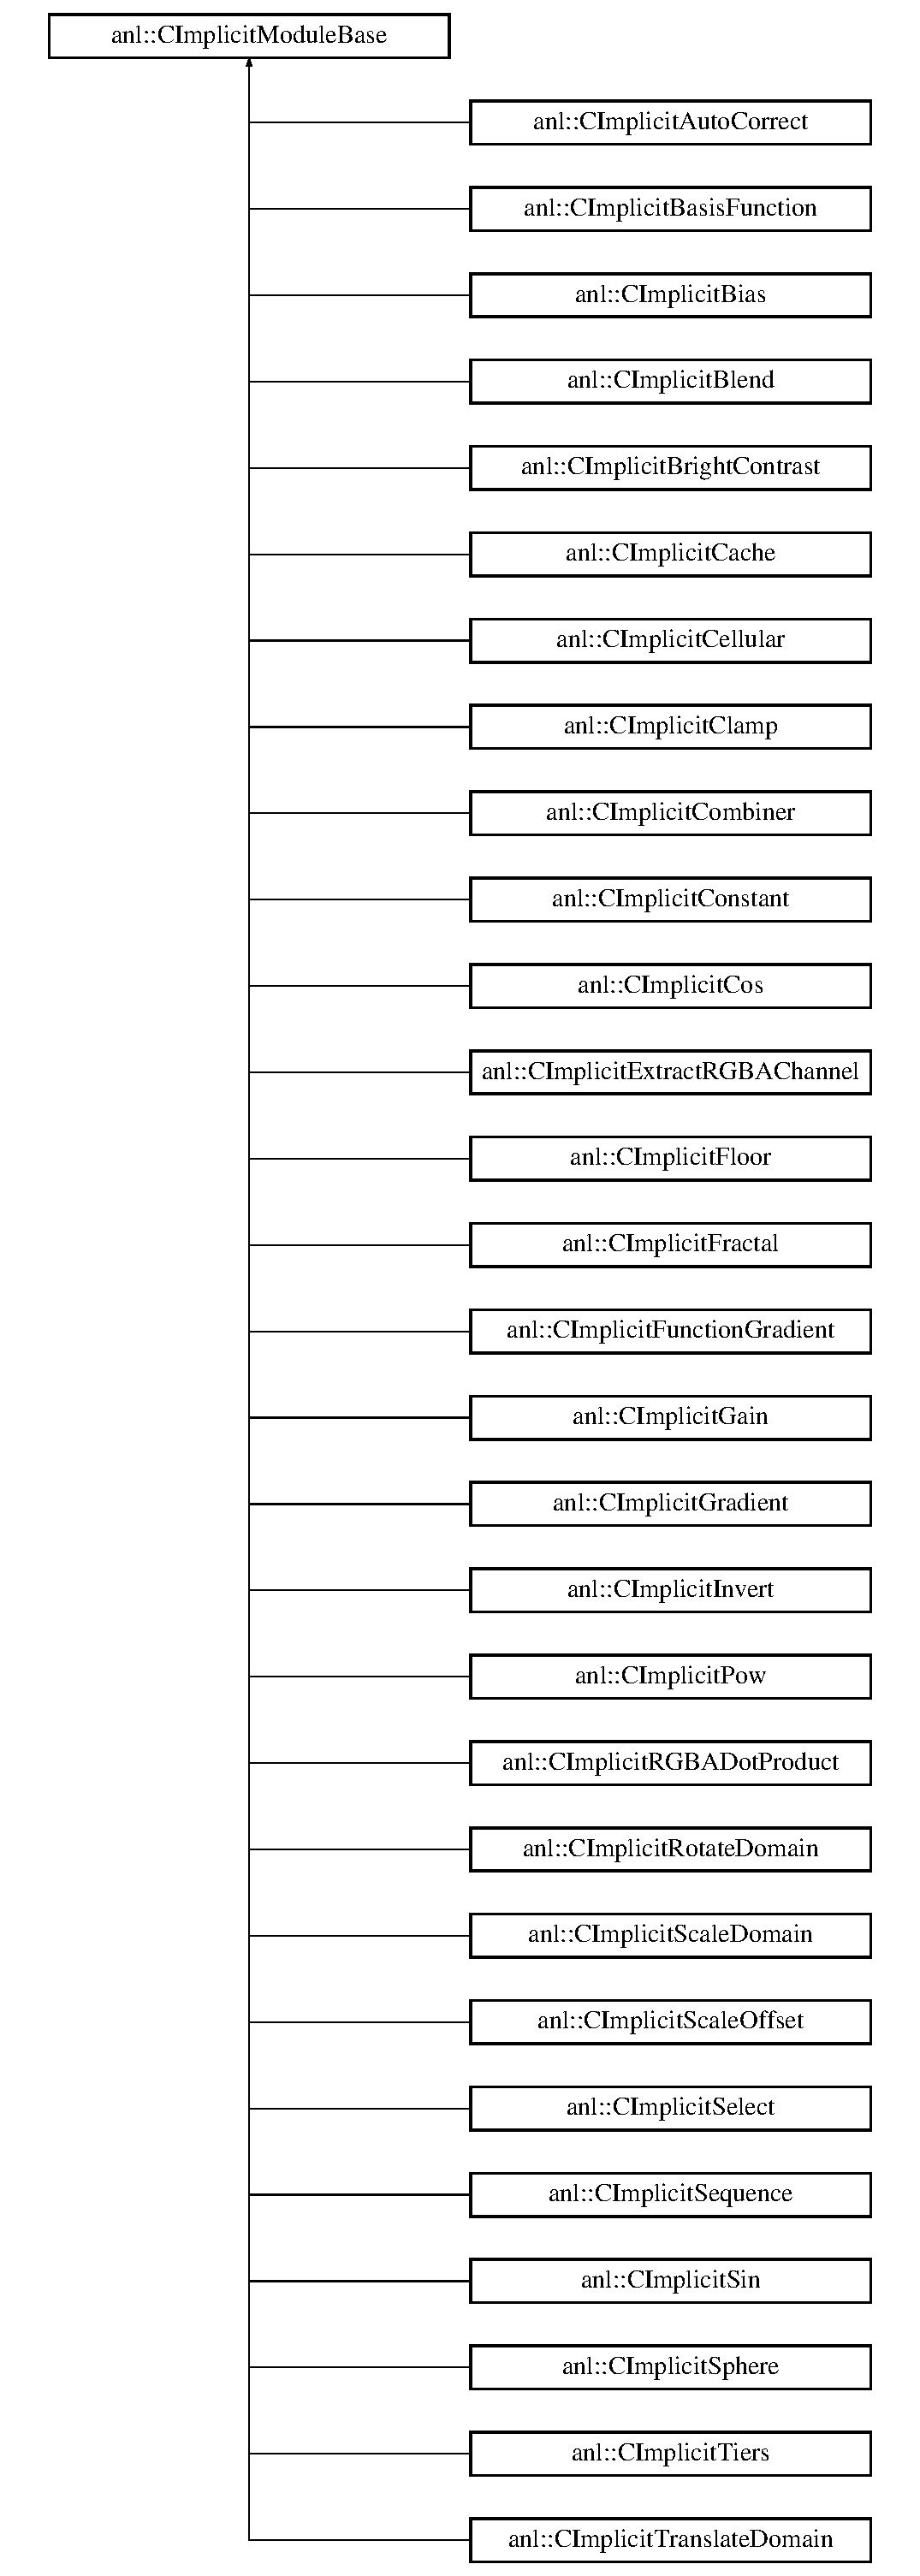
\includegraphics[height=12cm]{classanl_1_1CImplicitModuleBase}
\end{center}
\end{figure}
\subsection*{Public Types}
\begin{DoxyCompactItemize}
\item 
typedef std::function$<$ void(int)$>$ \hyperlink{classanl_1_1CImplicitModuleBase_a0af03005949051c16a5c063dd73b5eb8}{int\_\-v}
\item 
typedef std::function$<$ void(double)$>$ \hyperlink{classanl_1_1CImplicitModuleBase_a32d06aeb408b2063f45ad8c1d455e16c}{double\_\-v}
\item 
typedef std::function$<$ void(\hyperlink{classanl_1_1CImplicitModuleBase}{anl::CImplicitModuleBase} $\ast$) \hyperlink{classanl_1_1CImplicitModuleBase_a29276d273677a9928320cfb6118de3ba}{noise\_\-v} )
\end{DoxyCompactItemize}
\subsection*{Public Member Functions}
\begin{DoxyCompactItemize}
\item 
\hyperlink{classanl_1_1CImplicitModuleBase_a2179d89decfc65ec3f7dc2bfea98372d}{CImplicitModuleBase} ()
\item 
virtual \hyperlink{classanl_1_1CImplicitModuleBase_aa048225a76c86233b476ca598ed1cb01}{$\sim$CImplicitModuleBase} ()
\item 
virtual void \hyperlink{classanl_1_1CImplicitModuleBase_a12e7dc121de7ff95dd1952af2679867c}{setSeed} (unsigned int seed)
\item 
virtual double \hyperlink{classanl_1_1CImplicitModuleBase_ab88f8a1822dcfbc13ba5230318b0acd1}{get} (double x, double y)=0
\item 
virtual double \hyperlink{classanl_1_1CImplicitModuleBase_ac17d592612c82ba3d47f9229a00b1fe3}{get} (double x, double y, double z)=0
\item 
virtual double \hyperlink{classanl_1_1CImplicitModuleBase_a3cf520bdab59631864253c03b4e1723f}{get} (double x, double y, double z, double w)=0
\item 
virtual double \hyperlink{classanl_1_1CImplicitModuleBase_aa40b7d54572197612a4fea44b63447eb}{get} (double x, double y, double z, double w, double u, double v)=0
\item 
bool \hyperlink{classanl_1_1CImplicitModuleBase_ab86eb749d539e8282219e0f05de9c96c}{registerDoubleInput} (std::string const \&key, \hyperlink{classanl_1_1CImplicitModuleBase_a32d06aeb408b2063f45ad8c1d455e16c}{double\_\-v} const \&input)
\item 
bool \hyperlink{classanl_1_1CImplicitModuleBase_ac4143972345effb4c616e04b885d1076}{registerIntInput} (std::string const \&key, \hyperlink{classanl_1_1CImplicitModuleBase_a0af03005949051c16a5c063dd73b5eb8}{int\_\-v} const \&input)
\item 
bool \hyperlink{classanl_1_1CImplicitModuleBase_a830c5360e7cac6e4bd2c804105776dad}{registerNoiseInput} (std::string const \&key, \hyperlink{classanl_1_1CImplicitModuleBase_a29276d273677a9928320cfb6118de3ba}{noise\_\-v} const \&input)
\item 
void \hyperlink{classanl_1_1CImplicitModuleBase_a972deba664b63faa952dd5ecd381d36e}{setDoubleInput} (std::string key, double value)
\item 
void \hyperlink{classanl_1_1CImplicitModuleBase_afb474ef41f9f12afe1dd91317d8d9e9c}{setIntInput} (std::string key, int value)
\item 
void \hyperlink{classanl_1_1CImplicitModuleBase_a861c1b40199365605ec76d155ac4ea4c}{setNoiseInput} (std::string key, \hyperlink{classanl_1_1CImplicitModuleBase}{anl::CImplicitModuleBase} $\ast$value)
\end{DoxyCompactItemize}
\subsection*{Private Attributes}
\begin{DoxyCompactItemize}
\item 
std::map$<$ std::string, \hyperlink{classanl_1_1CImplicitModuleBase_a32d06aeb408b2063f45ad8c1d455e16c}{double\_\-v} $>$ \hyperlink{classanl_1_1CImplicitModuleBase_a44d78c30f32d9def6ad5a28f3831e5cb}{doubleFunctions}
\item 
std::map$<$ std::string, \hyperlink{classanl_1_1CImplicitModuleBase_a0af03005949051c16a5c063dd73b5eb8}{int\_\-v} $>$ \hyperlink{classanl_1_1CImplicitModuleBase_a6b667cd64feb2e8345fcf68eadc565e3}{intFunctions}
\item 
std::map$<$ std::string, \hyperlink{classanl_1_1CImplicitModuleBase_a29276d273677a9928320cfb6118de3ba}{noise\_\-v} $>$ \hyperlink{classanl_1_1CImplicitModuleBase_abeee324fb88e1ea014ac6595b9a98d16}{noiseFunctions}
\end{DoxyCompactItemize}


\subsection{Member Typedef Documentation}
\hypertarget{classanl_1_1CImplicitModuleBase_a32d06aeb408b2063f45ad8c1d455e16c}{
\index{anl::CImplicitModuleBase@{anl::CImplicitModuleBase}!double\_\-v@{double\_\-v}}
\index{double\_\-v@{double\_\-v}!anl::CImplicitModuleBase@{anl::CImplicitModuleBase}}
\subsubsection[{double\_\-v}]{\setlength{\rightskip}{0pt plus 5cm}typedef std::function$<$void(double)$>$ {\bf anl::CImplicitModuleBase::double\_\-v}}}
\label{classanl_1_1CImplicitModuleBase_a32d06aeb408b2063f45ad8c1d455e16c}
\hypertarget{classanl_1_1CImplicitModuleBase_a0af03005949051c16a5c063dd73b5eb8}{
\index{anl::CImplicitModuleBase@{anl::CImplicitModuleBase}!int\_\-v@{int\_\-v}}
\index{int\_\-v@{int\_\-v}!anl::CImplicitModuleBase@{anl::CImplicitModuleBase}}
\subsubsection[{int\_\-v}]{\setlength{\rightskip}{0pt plus 5cm}typedef std::function$<$void(int)$>$ {\bf anl::CImplicitModuleBase::int\_\-v}}}
\label{classanl_1_1CImplicitModuleBase_a0af03005949051c16a5c063dd73b5eb8}
\hypertarget{classanl_1_1CImplicitModuleBase_a29276d273677a9928320cfb6118de3ba}{
\index{anl::CImplicitModuleBase@{anl::CImplicitModuleBase}!noise\_\-v@{noise\_\-v}}
\index{noise\_\-v@{noise\_\-v}!anl::CImplicitModuleBase@{anl::CImplicitModuleBase}}
\subsubsection[{noise\_\-v}]{\setlength{\rightskip}{0pt plus 5cm}typedef std::function$<$void({\bf anl::CImplicitModuleBase}$\ast$) {\bf anl::CImplicitModuleBase::noise\_\-v})}}
\label{classanl_1_1CImplicitModuleBase_a29276d273677a9928320cfb6118de3ba}


\subsection{Constructor \& Destructor Documentation}
\hypertarget{classanl_1_1CImplicitModuleBase_a2179d89decfc65ec3f7dc2bfea98372d}{
\index{anl::CImplicitModuleBase@{anl::CImplicitModuleBase}!CImplicitModuleBase@{CImplicitModuleBase}}
\index{CImplicitModuleBase@{CImplicitModuleBase}!anl::CImplicitModuleBase@{anl::CImplicitModuleBase}}
\subsubsection[{CImplicitModuleBase}]{\setlength{\rightskip}{0pt plus 5cm}anl::CImplicitModuleBase::CImplicitModuleBase ()\hspace{0.3cm}{\ttfamily  \mbox{[}inline\mbox{]}}}}
\label{classanl_1_1CImplicitModuleBase_a2179d89decfc65ec3f7dc2bfea98372d}
\hypertarget{classanl_1_1CImplicitModuleBase_aa048225a76c86233b476ca598ed1cb01}{
\index{anl::CImplicitModuleBase@{anl::CImplicitModuleBase}!$\sim$CImplicitModuleBase@{$\sim$CImplicitModuleBase}}
\index{$\sim$CImplicitModuleBase@{$\sim$CImplicitModuleBase}!anl::CImplicitModuleBase@{anl::CImplicitModuleBase}}
\subsubsection[{$\sim$CImplicitModuleBase}]{\setlength{\rightskip}{0pt plus 5cm}virtual anl::CImplicitModuleBase::$\sim$CImplicitModuleBase ()\hspace{0.3cm}{\ttfamily  \mbox{[}inline, virtual\mbox{]}}}}
\label{classanl_1_1CImplicitModuleBase_aa048225a76c86233b476ca598ed1cb01}


\subsection{Member Function Documentation}
\hypertarget{classanl_1_1CImplicitModuleBase_aa40b7d54572197612a4fea44b63447eb}{
\index{anl::CImplicitModuleBase@{anl::CImplicitModuleBase}!get@{get}}
\index{get@{get}!anl::CImplicitModuleBase@{anl::CImplicitModuleBase}}
\subsubsection[{get}]{\setlength{\rightskip}{0pt plus 5cm}virtual double anl::CImplicitModuleBase::get (double {\em x}, \/  double {\em y}, \/  double {\em z}, \/  double {\em w}, \/  double {\em u}, \/  double {\em v})\hspace{0.3cm}{\ttfamily  \mbox{[}pure virtual\mbox{]}}}}
\label{classanl_1_1CImplicitModuleBase_aa40b7d54572197612a4fea44b63447eb}


Implemented in \hyperlink{classanl_1_1CImplicitAutoCorrect_ade9981b74d7798d6ad2840f57c191d45}{anl::CImplicitAutoCorrect}, \hyperlink{classanl_1_1CImplicitBasisFunction_a7841eca7a861e9bc6885b7a1c316c4df}{anl::CImplicitBasisFunction}, \hyperlink{classanl_1_1CImplicitBias_a8ca95f9d44c9c86a4d79a08906d6b029}{anl::CImplicitBias}, \hyperlink{classanl_1_1CImplicitBlend_a9d40ee4d97dac37b2a6aea498c7b7418}{anl::CImplicitBlend}, \hyperlink{classanl_1_1CImplicitBrightContrast_afeb937d994d492fa69cbbe61bdc8adfc}{anl::CImplicitBrightContrast}, \hyperlink{classanl_1_1CImplicitCache_ab7cae239c57e693521e2038461a2f5bb}{anl::CImplicitCache}, \hyperlink{classanl_1_1CImplicitCellular_a0d5bebde497611f47083b97220ecffef}{anl::CImplicitCellular}, \hyperlink{classanl_1_1CImplicitClamp_aaa9e4cef1586ec11c49dff2c6563aeea}{anl::CImplicitClamp}, \hyperlink{classanl_1_1CImplicitCombiner_ad4b8babff3aebe409e931a4453c0f617}{anl::CImplicitCombiner}, \hyperlink{classanl_1_1CImplicitConstant_a9f07f5043ff85ae39e0e484887a070d1}{anl::CImplicitConstant}, \hyperlink{classanl_1_1CImplicitCos_ad96831fb125b4c63bd17cd5f8064a64f}{anl::CImplicitCos}, \hyperlink{classanl_1_1CImplicitExtractRGBAChannel_a34f8c1bbb5757b600f96ef5bc18f5f70}{anl::CImplicitExtractRGBAChannel}, \hyperlink{classanl_1_1CImplicitFloor_af923d68186937208d6d877f69c1ab2dc}{anl::CImplicitFloor}, \hyperlink{classanl_1_1CImplicitFractal_ad70eef24b8616b72b7319f10cc1be82d}{anl::CImplicitFractal}, \hyperlink{classanl_1_1CImplicitFunctionGradient_ad37b8c002f1b4b44f0dd8af144fa59a8}{anl::CImplicitFunctionGradient}, \hyperlink{classanl_1_1CImplicitGain_a018e5eb3dae755a618400bfeb7798c7c}{anl::CImplicitGain}, \hyperlink{classanl_1_1CImplicitGradient_a00c49e418fae08368f1fb1a915c760e9}{anl::CImplicitGradient}, \hyperlink{classanl_1_1CImplicitInvert_aa09f4c5c466e8c83b0125260363d23bc}{anl::CImplicitInvert}, \hyperlink{classanl_1_1CImplicitPow_abb17667145906c16e125ec7c5fb86461}{anl::CImplicitPow}, \hyperlink{classanl_1_1CImplicitRGBADotProduct_a8ffc86bb80adb25aa80ae93e6269d394}{anl::CImplicitRGBADotProduct}, \hyperlink{classanl_1_1CImplicitRotateDomain_a17c9e93ed5a749c490da923c5faf1952}{anl::CImplicitRotateDomain}, \hyperlink{classanl_1_1CImplicitScaleDomain_aed69393e0a156ec2c0bf385b3e9345e7}{anl::CImplicitScaleDomain}, \hyperlink{classanl_1_1CImplicitScaleOffset_a5e048c2abd25d3b6ba95838fa1c7712d}{anl::CImplicitScaleOffset}, \hyperlink{classanl_1_1CImplicitSelect_ab66ac3d292721897bb15009585dc4190}{anl::CImplicitSelect}, \hyperlink{classanl_1_1CImplicitSequence_ad4333da8f7c124beb652a2de7b637753}{anl::CImplicitSequence}, \hyperlink{classanl_1_1CImplicitSin_ace607a9e9526483fe588e3e7355e1b77}{anl::CImplicitSin}, \hyperlink{classanl_1_1CImplicitSphere_a7f6bae7c64d5ff6f0472aa497f216237}{anl::CImplicitSphere}, \hyperlink{classanl_1_1CImplicitTiers_a0b150115944a998eac7c87ea937c1f89}{anl::CImplicitTiers}, and \hyperlink{classanl_1_1CImplicitTranslateDomain_a7d92931fb9633a1831a7303ca433546d}{anl::CImplicitTranslateDomain}.\hypertarget{classanl_1_1CImplicitModuleBase_a3cf520bdab59631864253c03b4e1723f}{
\index{anl::CImplicitModuleBase@{anl::CImplicitModuleBase}!get@{get}}
\index{get@{get}!anl::CImplicitModuleBase@{anl::CImplicitModuleBase}}
\subsubsection[{get}]{\setlength{\rightskip}{0pt plus 5cm}virtual double anl::CImplicitModuleBase::get (double {\em x}, \/  double {\em y}, \/  double {\em z}, \/  double {\em w})\hspace{0.3cm}{\ttfamily  \mbox{[}pure virtual\mbox{]}}}}
\label{classanl_1_1CImplicitModuleBase_a3cf520bdab59631864253c03b4e1723f}


Implemented in \hyperlink{classanl_1_1CImplicitAutoCorrect_a6f0ceb8d4b002577185b2004c77f9375}{anl::CImplicitAutoCorrect}, \hyperlink{classanl_1_1CImplicitBasisFunction_a5dab3e931e2bffd223301ada4e9080ef}{anl::CImplicitBasisFunction}, \hyperlink{classanl_1_1CImplicitBias_a9b033816e96601675dd0d9abdd56df4e}{anl::CImplicitBias}, \hyperlink{classanl_1_1CImplicitBlend_ac3d285ae9ab47e299c706b2357e3b179}{anl::CImplicitBlend}, \hyperlink{classanl_1_1CImplicitBrightContrast_a8b2497875f7c2d22cc723673358c3463}{anl::CImplicitBrightContrast}, \hyperlink{classanl_1_1CImplicitCache_a0f5dff0ad736097091e6c02272701393}{anl::CImplicitCache}, \hyperlink{classanl_1_1CImplicitCellular_aaa7f9b16d76ba2fd6e8c1105ea76ba1e}{anl::CImplicitCellular}, \hyperlink{classanl_1_1CImplicitClamp_a2ccd309fe3a92eb4e5aaa9f5921b6be3}{anl::CImplicitClamp}, \hyperlink{classanl_1_1CImplicitCombiner_aaaeeee91ac651cd74432806f8533d9e6}{anl::CImplicitCombiner}, \hyperlink{classanl_1_1CImplicitConstant_a90c57419a55ae0914447f7bf325ca27e}{anl::CImplicitConstant}, \hyperlink{classanl_1_1CImplicitCos_aa9326ba121ca49ae6caf52e7143020a7}{anl::CImplicitCos}, \hyperlink{classanl_1_1CImplicitExtractRGBAChannel_a89cec90ae47f3210f1e12f647514d1c2}{anl::CImplicitExtractRGBAChannel}, \hyperlink{classanl_1_1CImplicitFloor_ae6b0c4cf4b5616de73ff319cc976e701}{anl::CImplicitFloor}, \hyperlink{classanl_1_1CImplicitFractal_a39627567ff6ca149513d0870592f1f8e}{anl::CImplicitFractal}, \hyperlink{classanl_1_1CImplicitFunctionGradient_a31fceb058f6c34b8f63d463de1f3f9a6}{anl::CImplicitFunctionGradient}, \hyperlink{classanl_1_1CImplicitGain_a2d1715d0d153cc6a6e0a0154484fe90c}{anl::CImplicitGain}, \hyperlink{classanl_1_1CImplicitGradient_a49c3b137f2ee2a713de213d949c2c05a}{anl::CImplicitGradient}, \hyperlink{classanl_1_1CImplicitInvert_aa27168b58b90f1f84e199343de0a91a7}{anl::CImplicitInvert}, \hyperlink{classanl_1_1CImplicitPow_a541948e854797b149ff0c9a29599d50d}{anl::CImplicitPow}, \hyperlink{classanl_1_1CImplicitRGBADotProduct_ac38f2572f66e335ce9bb1e59b2fc7199}{anl::CImplicitRGBADotProduct}, \hyperlink{classanl_1_1CImplicitRotateDomain_a094b57aa7d2acfbe3c069540a546be0d}{anl::CImplicitRotateDomain}, \hyperlink{classanl_1_1CImplicitScaleDomain_af53d0c59728d29e9b8cd21b581030b24}{anl::CImplicitScaleDomain}, \hyperlink{classanl_1_1CImplicitScaleOffset_a8ac84534b65230172a9f2e61fbfaa0ae}{anl::CImplicitScaleOffset}, \hyperlink{classanl_1_1CImplicitSelect_ac0b010e48784974a4c7d9639a9a6f84e}{anl::CImplicitSelect}, \hyperlink{classanl_1_1CImplicitSequence_a1db8e15397e9bf75176b5f24d57befac}{anl::CImplicitSequence}, \hyperlink{classanl_1_1CImplicitSin_a5f666f8ad48fa7337524c304b63c8a1f}{anl::CImplicitSin}, \hyperlink{classanl_1_1CImplicitSphere_a08193959ed4c6390025032da175f90ec}{anl::CImplicitSphere}, \hyperlink{classanl_1_1CImplicitTiers_a7bb007d1a541d37b5d48027a932f4117}{anl::CImplicitTiers}, and \hyperlink{classanl_1_1CImplicitTranslateDomain_a4c5022a45953ac556e169e2186bf9105}{anl::CImplicitTranslateDomain}.\hypertarget{classanl_1_1CImplicitModuleBase_ac17d592612c82ba3d47f9229a00b1fe3}{
\index{anl::CImplicitModuleBase@{anl::CImplicitModuleBase}!get@{get}}
\index{get@{get}!anl::CImplicitModuleBase@{anl::CImplicitModuleBase}}
\subsubsection[{get}]{\setlength{\rightskip}{0pt plus 5cm}virtual double anl::CImplicitModuleBase::get (double {\em x}, \/  double {\em y}, \/  double {\em z})\hspace{0.3cm}{\ttfamily  \mbox{[}pure virtual\mbox{]}}}}
\label{classanl_1_1CImplicitModuleBase_ac17d592612c82ba3d47f9229a00b1fe3}


Implemented in \hyperlink{classanl_1_1CImplicitAutoCorrect_a8b9fafdbf1e508a461d8fca1e60172eb}{anl::CImplicitAutoCorrect}, \hyperlink{classanl_1_1CImplicitBasisFunction_af4ae388cbc87477600c5d24c2450366b}{anl::CImplicitBasisFunction}, \hyperlink{classanl_1_1CImplicitBias_a31ad13c0e8b41f5d8b8df9d93f22501d}{anl::CImplicitBias}, \hyperlink{classanl_1_1CImplicitBlend_a446d55152cda96d074d03055383c7f0d}{anl::CImplicitBlend}, \hyperlink{classanl_1_1CImplicitBrightContrast_a545704ba2a73a8b58e5e07751a706f3a}{anl::CImplicitBrightContrast}, \hyperlink{classanl_1_1CImplicitCache_aaf9fc4aff6c39b2e0815d6c285dc478f}{anl::CImplicitCache}, \hyperlink{classanl_1_1CImplicitCellular_aefaad448623f73921542503bc6ef898a}{anl::CImplicitCellular}, \hyperlink{classanl_1_1CImplicitClamp_ac35e4acee06cf5ad4ab4db236bcf8672}{anl::CImplicitClamp}, \hyperlink{classanl_1_1CImplicitCombiner_a44bf6015e5f1895cc494ed7188401172}{anl::CImplicitCombiner}, \hyperlink{classanl_1_1CImplicitConstant_a92a9154b9dee96b7c01637d9b8f879de}{anl::CImplicitConstant}, \hyperlink{classanl_1_1CImplicitCos_a4b8b0150cfffc6e066fc4e62cb2dd33e}{anl::CImplicitCos}, \hyperlink{classanl_1_1CImplicitExtractRGBAChannel_ad9ffeeea3e53af27d4c2fd3dc81ea1bc}{anl::CImplicitExtractRGBAChannel}, \hyperlink{classanl_1_1CImplicitFloor_ae73876cea1480c84adc05b83cca26255}{anl::CImplicitFloor}, \hyperlink{classanl_1_1CImplicitFractal_a25ac928857e827545123d8f5098e5131}{anl::CImplicitFractal}, \hyperlink{classanl_1_1CImplicitFunctionGradient_a4844ed9eeaa55d149d5f918915a54f12}{anl::CImplicitFunctionGradient}, \hyperlink{classanl_1_1CImplicitGain_a76cf906f9e4bd4a6346f368951215ca5}{anl::CImplicitGain}, \hyperlink{classanl_1_1CImplicitGradient_ae9cba8a20bb633f73c94118d6a644d70}{anl::CImplicitGradient}, \hyperlink{classanl_1_1CImplicitInvert_ad6f8f7bbf36c6b7ef4fa024c316fd068}{anl::CImplicitInvert}, \hyperlink{classanl_1_1CImplicitPow_aad892840e7a9570d4ae0441cfbe61c4e}{anl::CImplicitPow}, \hyperlink{classanl_1_1CImplicitRGBADotProduct_aaf1fa4fa39be36a09dde553b73a14537}{anl::CImplicitRGBADotProduct}, \hyperlink{classanl_1_1CImplicitRotateDomain_a45697c6d5fcd6d5b551219a5520d0db8}{anl::CImplicitRotateDomain}, \hyperlink{classanl_1_1CImplicitScaleDomain_a7dfe0c88e39f22949a8233e60d0bf70c}{anl::CImplicitScaleDomain}, \hyperlink{classanl_1_1CImplicitScaleOffset_a1dbdceab30f5303f7fda0eb9a5ca1cdd}{anl::CImplicitScaleOffset}, \hyperlink{classanl_1_1CImplicitSelect_a324bded1a066192e2831cd7d80063cbc}{anl::CImplicitSelect}, \hyperlink{classanl_1_1CImplicitSequence_a9514300a86679a099eccee6b87bfd9c1}{anl::CImplicitSequence}, \hyperlink{classanl_1_1CImplicitSin_a5b61d1f4f70eab619edf3b7085cc0759}{anl::CImplicitSin}, \hyperlink{classanl_1_1CImplicitSphere_a8698af16bc095a14992560caf6be36c7}{anl::CImplicitSphere}, \hyperlink{classanl_1_1CImplicitTiers_a6b1cc8151e56b6c9c66da13be3f73a80}{anl::CImplicitTiers}, and \hyperlink{classanl_1_1CImplicitTranslateDomain_a875f867e25e0d9c5497b68ea5ef8c358}{anl::CImplicitTranslateDomain}.\hypertarget{classanl_1_1CImplicitModuleBase_ab88f8a1822dcfbc13ba5230318b0acd1}{
\index{anl::CImplicitModuleBase@{anl::CImplicitModuleBase}!get@{get}}
\index{get@{get}!anl::CImplicitModuleBase@{anl::CImplicitModuleBase}}
\subsubsection[{get}]{\setlength{\rightskip}{0pt plus 5cm}virtual double anl::CImplicitModuleBase::get (double {\em x}, \/  double {\em y})\hspace{0.3cm}{\ttfamily  \mbox{[}pure virtual\mbox{]}}}}
\label{classanl_1_1CImplicitModuleBase_ab88f8a1822dcfbc13ba5230318b0acd1}


Implemented in \hyperlink{classanl_1_1CImplicitAutoCorrect_a134b304eeb21068a96cbdcb8427af104}{anl::CImplicitAutoCorrect}, \hyperlink{classanl_1_1CImplicitBasisFunction_a78231e212255d16f3c99edd7107ae2da}{anl::CImplicitBasisFunction}, \hyperlink{classanl_1_1CImplicitBias_a7bc226cf7d835946936e76144e56a5b6}{anl::CImplicitBias}, \hyperlink{classanl_1_1CImplicitBlend_a24ce6a5991691901f1db4d8c7a78089e}{anl::CImplicitBlend}, \hyperlink{classanl_1_1CImplicitBrightContrast_a8b6d690936515565c8147eddcb2adbee}{anl::CImplicitBrightContrast}, \hyperlink{classanl_1_1CImplicitCache_a90f12b78d1a0b263d2fc142df64a52c9}{anl::CImplicitCache}, \hyperlink{classanl_1_1CImplicitCellular_aefb6e04efeb573a51112f1f27edef569}{anl::CImplicitCellular}, \hyperlink{classanl_1_1CImplicitClamp_a2729b466be78da8a56b90eee7c3a2436}{anl::CImplicitClamp}, \hyperlink{classanl_1_1CImplicitCombiner_a4fac6a4b68eea473c48b2c2cb914c2bd}{anl::CImplicitCombiner}, \hyperlink{classanl_1_1CImplicitConstant_afc877ea9b1b8f119f7aeea2dde8b8190}{anl::CImplicitConstant}, \hyperlink{classanl_1_1CImplicitCos_ad17b40e7a1bfee39e5c0bd103154cc22}{anl::CImplicitCos}, \hyperlink{classanl_1_1CImplicitExtractRGBAChannel_a8770c4c419956bfc7a1ddf7e40fe0c66}{anl::CImplicitExtractRGBAChannel}, \hyperlink{classanl_1_1CImplicitFloor_ad2a70f69657f5e662ce91f45e3a84a75}{anl::CImplicitFloor}, \hyperlink{classanl_1_1CImplicitFractal_a9ce533cdedbee58d917e8db1ab632d2f}{anl::CImplicitFractal}, \hyperlink{classanl_1_1CImplicitFunctionGradient_ab9f146161cbb8ab46ee5260467139c8b}{anl::CImplicitFunctionGradient}, \hyperlink{classanl_1_1CImplicitGain_af51697ea592424db9710d58a251b555e}{anl::CImplicitGain}, \hyperlink{classanl_1_1CImplicitGradient_a7e580d3643f735ba73177de4919935b7}{anl::CImplicitGradient}, \hyperlink{classanl_1_1CImplicitInvert_aa4dacdebefdd1721cdda423c41ec98b4}{anl::CImplicitInvert}, \hyperlink{classanl_1_1CImplicitPow_af8b092909ba5aaf13ce199477613a9e0}{anl::CImplicitPow}, \hyperlink{classanl_1_1CImplicitRGBADotProduct_ad2d4c06f27551fee761b9736689c971a}{anl::CImplicitRGBADotProduct}, \hyperlink{classanl_1_1CImplicitRotateDomain_a9599a3b576c39197f6807202c7679480}{anl::CImplicitRotateDomain}, \hyperlink{classanl_1_1CImplicitScaleDomain_a9f4a9bc6d4cf2af9209123423b83feec}{anl::CImplicitScaleDomain}, \hyperlink{classanl_1_1CImplicitScaleOffset_ac23178ec8ef455748dfc75684515c291}{anl::CImplicitScaleOffset}, \hyperlink{classanl_1_1CImplicitSelect_a0bc7db92ebc00afd8d195c31c207b234}{anl::CImplicitSelect}, \hyperlink{classanl_1_1CImplicitSequence_a332ee86290e47c570c30fa858b262a9c}{anl::CImplicitSequence}, \hyperlink{classanl_1_1CImplicitSin_a16e93edeebd6771c4a42c4c11939af19}{anl::CImplicitSin}, \hyperlink{classanl_1_1CImplicitSphere_a215221f358be39ffc2fd09ffe77ca7bc}{anl::CImplicitSphere}, \hyperlink{classanl_1_1CImplicitTiers_a497494a60352ce9490ddd28125beb01a}{anl::CImplicitTiers}, and \hyperlink{classanl_1_1CImplicitTranslateDomain_a8f0d141a02e5e67245d07ee30324d13d}{anl::CImplicitTranslateDomain}.\hypertarget{classanl_1_1CImplicitModuleBase_ab86eb749d539e8282219e0f05de9c96c}{
\index{anl::CImplicitModuleBase@{anl::CImplicitModuleBase}!registerDoubleInput@{registerDoubleInput}}
\index{registerDoubleInput@{registerDoubleInput}!anl::CImplicitModuleBase@{anl::CImplicitModuleBase}}
\subsubsection[{registerDoubleInput}]{\setlength{\rightskip}{0pt plus 5cm}bool anl::CImplicitModuleBase::registerDoubleInput (std::string const \& {\em key}, \/  {\bf double\_\-v} const \& {\em input})\hspace{0.3cm}{\ttfamily  \mbox{[}inline\mbox{]}}}}
\label{classanl_1_1CImplicitModuleBase_ab86eb749d539e8282219e0f05de9c96c}
\hypertarget{classanl_1_1CImplicitModuleBase_ac4143972345effb4c616e04b885d1076}{
\index{anl::CImplicitModuleBase@{anl::CImplicitModuleBase}!registerIntInput@{registerIntInput}}
\index{registerIntInput@{registerIntInput}!anl::CImplicitModuleBase@{anl::CImplicitModuleBase}}
\subsubsection[{registerIntInput}]{\setlength{\rightskip}{0pt plus 5cm}bool anl::CImplicitModuleBase::registerIntInput (std::string const \& {\em key}, \/  {\bf int\_\-v} const \& {\em input})\hspace{0.3cm}{\ttfamily  \mbox{[}inline\mbox{]}}}}
\label{classanl_1_1CImplicitModuleBase_ac4143972345effb4c616e04b885d1076}
\hypertarget{classanl_1_1CImplicitModuleBase_a830c5360e7cac6e4bd2c804105776dad}{
\index{anl::CImplicitModuleBase@{anl::CImplicitModuleBase}!registerNoiseInput@{registerNoiseInput}}
\index{registerNoiseInput@{registerNoiseInput}!anl::CImplicitModuleBase@{anl::CImplicitModuleBase}}
\subsubsection[{registerNoiseInput}]{\setlength{\rightskip}{0pt plus 5cm}bool anl::CImplicitModuleBase::registerNoiseInput (std::string const \& {\em key}, \/  {\bf noise\_\-v} const \& {\em input})\hspace{0.3cm}{\ttfamily  \mbox{[}inline\mbox{]}}}}
\label{classanl_1_1CImplicitModuleBase_a830c5360e7cac6e4bd2c804105776dad}
\hypertarget{classanl_1_1CImplicitModuleBase_a972deba664b63faa952dd5ecd381d36e}{
\index{anl::CImplicitModuleBase@{anl::CImplicitModuleBase}!setDoubleInput@{setDoubleInput}}
\index{setDoubleInput@{setDoubleInput}!anl::CImplicitModuleBase@{anl::CImplicitModuleBase}}
\subsubsection[{setDoubleInput}]{\setlength{\rightskip}{0pt plus 5cm}void anl::CImplicitModuleBase::setDoubleInput (std::string {\em key}, \/  double {\em value})\hspace{0.3cm}{\ttfamily  \mbox{[}inline\mbox{]}}}}
\label{classanl_1_1CImplicitModuleBase_a972deba664b63faa952dd5ecd381d36e}
\hypertarget{classanl_1_1CImplicitModuleBase_afb474ef41f9f12afe1dd91317d8d9e9c}{
\index{anl::CImplicitModuleBase@{anl::CImplicitModuleBase}!setIntInput@{setIntInput}}
\index{setIntInput@{setIntInput}!anl::CImplicitModuleBase@{anl::CImplicitModuleBase}}
\subsubsection[{setIntInput}]{\setlength{\rightskip}{0pt plus 5cm}void anl::CImplicitModuleBase::setIntInput (std::string {\em key}, \/  int {\em value})\hspace{0.3cm}{\ttfamily  \mbox{[}inline\mbox{]}}}}
\label{classanl_1_1CImplicitModuleBase_afb474ef41f9f12afe1dd91317d8d9e9c}
\hypertarget{classanl_1_1CImplicitModuleBase_a861c1b40199365605ec76d155ac4ea4c}{
\index{anl::CImplicitModuleBase@{anl::CImplicitModuleBase}!setNoiseInput@{setNoiseInput}}
\index{setNoiseInput@{setNoiseInput}!anl::CImplicitModuleBase@{anl::CImplicitModuleBase}}
\subsubsection[{setNoiseInput}]{\setlength{\rightskip}{0pt plus 5cm}void anl::CImplicitModuleBase::setNoiseInput (std::string {\em key}, \/  {\bf anl::CImplicitModuleBase} $\ast$ {\em value})\hspace{0.3cm}{\ttfamily  \mbox{[}inline\mbox{]}}}}
\label{classanl_1_1CImplicitModuleBase_a861c1b40199365605ec76d155ac4ea4c}
\hypertarget{classanl_1_1CImplicitModuleBase_a12e7dc121de7ff95dd1952af2679867c}{
\index{anl::CImplicitModuleBase@{anl::CImplicitModuleBase}!setSeed@{setSeed}}
\index{setSeed@{setSeed}!anl::CImplicitModuleBase@{anl::CImplicitModuleBase}}
\subsubsection[{setSeed}]{\setlength{\rightskip}{0pt plus 5cm}virtual void anl::CImplicitModuleBase::setSeed (unsigned int {\em seed})\hspace{0.3cm}{\ttfamily  \mbox{[}inline, virtual\mbox{]}}}}
\label{classanl_1_1CImplicitModuleBase_a12e7dc121de7ff95dd1952af2679867c}


Reimplemented in \hyperlink{classanl_1_1CImplicitBasisFunction_a1fba23e4d106edd9cdc44dd52e116d2d}{anl::CImplicitBasisFunction}, and \hyperlink{classanl_1_1CImplicitFractal_ad50523033bd36b13bbc21aaa3def0499}{anl::CImplicitFractal}.

\subsection{Field Documentation}
\hypertarget{classanl_1_1CImplicitModuleBase_a44d78c30f32d9def6ad5a28f3831e5cb}{
\index{anl::CImplicitModuleBase@{anl::CImplicitModuleBase}!doubleFunctions@{doubleFunctions}}
\index{doubleFunctions@{doubleFunctions}!anl::CImplicitModuleBase@{anl::CImplicitModuleBase}}
\subsubsection[{doubleFunctions}]{\setlength{\rightskip}{0pt plus 5cm}std::map$<$std::string, {\bf double\_\-v}$>$ {\bf anl::CImplicitModuleBase::doubleFunctions}\hspace{0.3cm}{\ttfamily  \mbox{[}private\mbox{]}}}}
\label{classanl_1_1CImplicitModuleBase_a44d78c30f32d9def6ad5a28f3831e5cb}
\hypertarget{classanl_1_1CImplicitModuleBase_a6b667cd64feb2e8345fcf68eadc565e3}{
\index{anl::CImplicitModuleBase@{anl::CImplicitModuleBase}!intFunctions@{intFunctions}}
\index{intFunctions@{intFunctions}!anl::CImplicitModuleBase@{anl::CImplicitModuleBase}}
\subsubsection[{intFunctions}]{\setlength{\rightskip}{0pt plus 5cm}std::map$<$std::string, {\bf int\_\-v}$>$ {\bf anl::CImplicitModuleBase::intFunctions}\hspace{0.3cm}{\ttfamily  \mbox{[}private\mbox{]}}}}
\label{classanl_1_1CImplicitModuleBase_a6b667cd64feb2e8345fcf68eadc565e3}
\hypertarget{classanl_1_1CImplicitModuleBase_abeee324fb88e1ea014ac6595b9a98d16}{
\index{anl::CImplicitModuleBase@{anl::CImplicitModuleBase}!noiseFunctions@{noiseFunctions}}
\index{noiseFunctions@{noiseFunctions}!anl::CImplicitModuleBase@{anl::CImplicitModuleBase}}
\subsubsection[{noiseFunctions}]{\setlength{\rightskip}{0pt plus 5cm}std::map$<$std::string, {\bf noise\_\-v}$>$ {\bf anl::CImplicitModuleBase::noiseFunctions}\hspace{0.3cm}{\ttfamily  \mbox{[}private\mbox{]}}}}
\label{classanl_1_1CImplicitModuleBase_abeee324fb88e1ea014ac6595b9a98d16}


The documentation for this class was generated from the following file:\begin{DoxyCompactItemize}
\item 
include/\hyperlink{implicitmodulebase_8h}{implicitmodulebase.h}\end{DoxyCompactItemize}

\hypertarget{structanl_1_1CImplicitModuleFactory}{
\section{anl::CImplicitModuleFactory Struct Reference}
\label{structanl_1_1CImplicitModuleFactory}\index{anl::CImplicitModuleFactory@{anl::CImplicitModuleFactory}}
}


{\ttfamily \#include $<$implicitmodulebase.h$>$}Inheritance diagram for anl::CImplicitModuleFactory::\begin{figure}[H]
\begin{center}
\leavevmode
\includegraphics[height=2cm]{structanl_1_1CImplicitModuleFactory}
\end{center}
\end{figure}
\subsection*{Static Public Member Functions}
\begin{DoxyCompactItemize}
\item 
static \hyperlink{structanl_1_1CImplicitModuleFactory}{CImplicitModuleFactory} \& \hyperlink{structanl_1_1CImplicitModuleFactory_a0ee63f8dd3d2e8fc53a25d1fd765f34a}{instance} ()
\end{DoxyCompactItemize}


\subsection{Member Function Documentation}
\hypertarget{structanl_1_1CImplicitModuleFactory_a0ee63f8dd3d2e8fc53a25d1fd765f34a}{
\index{anl::CImplicitModuleFactory@{anl::CImplicitModuleFactory}!instance@{instance}}
\index{instance@{instance}!anl::CImplicitModuleFactory@{anl::CImplicitModuleFactory}}
\subsubsection[{instance}]{\setlength{\rightskip}{0pt plus 5cm}static {\bf CImplicitModuleFactory}\& anl::CImplicitModuleFactory::instance ()\hspace{0.3cm}{\ttfamily  \mbox{[}inline, static\mbox{]}}}}
\label{structanl_1_1CImplicitModuleFactory_a0ee63f8dd3d2e8fc53a25d1fd765f34a}


The documentation for this struct was generated from the following file:\begin{DoxyCompactItemize}
\item 
include/\hyperlink{implicitmodulebase_8h}{implicitmodulebase.h}\end{DoxyCompactItemize}

\hypertarget{classanl_1_1CImplicitPow}{
\section{anl::CImplicitPow Class Reference}
\label{classanl_1_1CImplicitPow}\index{anl::CImplicitPow@{anl::CImplicitPow}}
}


{\ttfamily \#include $<$implicitpow.h$>$}Inheritance diagram for anl::CImplicitPow::\begin{figure}[H]
\begin{center}
\leavevmode
\includegraphics[height=2cm]{classanl_1_1CImplicitPow}
\end{center}
\end{figure}
\subsection*{Public Member Functions}
\begin{DoxyCompactItemize}
\item 
\hyperlink{classanl_1_1CImplicitPow_afa3eb17e6b117bae52797598a1d223b2}{CImplicitPow} ()
\item 
\hyperlink{classanl_1_1CImplicitPow_afa502e9f519d89a836f163cd5ac8fb3a}{$\sim$CImplicitPow} ()
\item 
void \hyperlink{classanl_1_1CImplicitPow_ac717e60af1d88a41b3d48c3da2430c76}{setSource} (double v)
\item 
void \hyperlink{classanl_1_1CImplicitPow_a596142e97efeeff173835acda522e933}{setSource} (\hyperlink{classanl_1_1CImplicitModuleBase}{CImplicitModuleBase} $\ast$m)
\item 
void \hyperlink{classanl_1_1CImplicitPow_ae7c4bf26ecc28386101c22c3628e2ca6}{setPower} (double v)
\item 
void \hyperlink{classanl_1_1CImplicitPow_a663be4a5421ffcd2dbf2d41574dec821}{setPower} (\hyperlink{classanl_1_1CImplicitModuleBase}{CImplicitModuleBase} $\ast$m)
\item 
double \hyperlink{classanl_1_1CImplicitPow_af8b092909ba5aaf13ce199477613a9e0}{get} (double x, double y)
\item 
double \hyperlink{classanl_1_1CImplicitPow_aad892840e7a9570d4ae0441cfbe61c4e}{get} (double x, double y, double z)
\item 
double \hyperlink{classanl_1_1CImplicitPow_a541948e854797b149ff0c9a29599d50d}{get} (double x, double y, double z, double w)
\item 
double \hyperlink{classanl_1_1CImplicitPow_abb17667145906c16e125ec7c5fb86461}{get} (double x, double y, double z, double w, double u, double v)
\end{DoxyCompactItemize}
\subsection*{Protected Attributes}
\begin{DoxyCompactItemize}
\item 
\hyperlink{classanl_1_1CScalarParameter}{CScalarParameter} \hyperlink{classanl_1_1CImplicitPow_aae11a9a743adf6158fe9190f2f358538}{m\_\-source}
\item 
\hyperlink{classanl_1_1CScalarParameter}{CScalarParameter} \hyperlink{classanl_1_1CImplicitPow_a583a37c58658b696b7352bb111429de5}{m\_\-power}
\end{DoxyCompactItemize}


\subsection{Constructor \& Destructor Documentation}
\hypertarget{classanl_1_1CImplicitPow_afa3eb17e6b117bae52797598a1d223b2}{
\index{anl::CImplicitPow@{anl::CImplicitPow}!CImplicitPow@{CImplicitPow}}
\index{CImplicitPow@{CImplicitPow}!anl::CImplicitPow@{anl::CImplicitPow}}
\subsubsection[{CImplicitPow}]{\setlength{\rightskip}{0pt plus 5cm}anl::CImplicitPow::CImplicitPow ()}}
\label{classanl_1_1CImplicitPow_afa3eb17e6b117bae52797598a1d223b2}
\hypertarget{classanl_1_1CImplicitPow_afa502e9f519d89a836f163cd5ac8fb3a}{
\index{anl::CImplicitPow@{anl::CImplicitPow}!$\sim$CImplicitPow@{$\sim$CImplicitPow}}
\index{$\sim$CImplicitPow@{$\sim$CImplicitPow}!anl::CImplicitPow@{anl::CImplicitPow}}
\subsubsection[{$\sim$CImplicitPow}]{\setlength{\rightskip}{0pt plus 5cm}anl::CImplicitPow::$\sim$CImplicitPow ()}}
\label{classanl_1_1CImplicitPow_afa502e9f519d89a836f163cd5ac8fb3a}


\subsection{Member Function Documentation}
\hypertarget{classanl_1_1CImplicitPow_abb17667145906c16e125ec7c5fb86461}{
\index{anl::CImplicitPow@{anl::CImplicitPow}!get@{get}}
\index{get@{get}!anl::CImplicitPow@{anl::CImplicitPow}}
\subsubsection[{get}]{\setlength{\rightskip}{0pt plus 5cm}double anl::CImplicitPow::get (double {\em x}, \/  double {\em y}, \/  double {\em z}, \/  double {\em w}, \/  double {\em u}, \/  double {\em v})\hspace{0.3cm}{\ttfamily  \mbox{[}virtual\mbox{]}}}}
\label{classanl_1_1CImplicitPow_abb17667145906c16e125ec7c5fb86461}


Implements \hyperlink{classanl_1_1CImplicitModuleBase_aa40b7d54572197612a4fea44b63447eb}{anl::CImplicitModuleBase}.\hypertarget{classanl_1_1CImplicitPow_a541948e854797b149ff0c9a29599d50d}{
\index{anl::CImplicitPow@{anl::CImplicitPow}!get@{get}}
\index{get@{get}!anl::CImplicitPow@{anl::CImplicitPow}}
\subsubsection[{get}]{\setlength{\rightskip}{0pt plus 5cm}double anl::CImplicitPow::get (double {\em x}, \/  double {\em y}, \/  double {\em z}, \/  double {\em w})\hspace{0.3cm}{\ttfamily  \mbox{[}virtual\mbox{]}}}}
\label{classanl_1_1CImplicitPow_a541948e854797b149ff0c9a29599d50d}


Implements \hyperlink{classanl_1_1CImplicitModuleBase_a3cf520bdab59631864253c03b4e1723f}{anl::CImplicitModuleBase}.\hypertarget{classanl_1_1CImplicitPow_aad892840e7a9570d4ae0441cfbe61c4e}{
\index{anl::CImplicitPow@{anl::CImplicitPow}!get@{get}}
\index{get@{get}!anl::CImplicitPow@{anl::CImplicitPow}}
\subsubsection[{get}]{\setlength{\rightskip}{0pt plus 5cm}double anl::CImplicitPow::get (double {\em x}, \/  double {\em y}, \/  double {\em z})\hspace{0.3cm}{\ttfamily  \mbox{[}virtual\mbox{]}}}}
\label{classanl_1_1CImplicitPow_aad892840e7a9570d4ae0441cfbe61c4e}


Implements \hyperlink{classanl_1_1CImplicitModuleBase_ac17d592612c82ba3d47f9229a00b1fe3}{anl::CImplicitModuleBase}.\hypertarget{classanl_1_1CImplicitPow_af8b092909ba5aaf13ce199477613a9e0}{
\index{anl::CImplicitPow@{anl::CImplicitPow}!get@{get}}
\index{get@{get}!anl::CImplicitPow@{anl::CImplicitPow}}
\subsubsection[{get}]{\setlength{\rightskip}{0pt plus 5cm}double anl::CImplicitPow::get (double {\em x}, \/  double {\em y})\hspace{0.3cm}{\ttfamily  \mbox{[}virtual\mbox{]}}}}
\label{classanl_1_1CImplicitPow_af8b092909ba5aaf13ce199477613a9e0}


Implements \hyperlink{classanl_1_1CImplicitModuleBase_ab88f8a1822dcfbc13ba5230318b0acd1}{anl::CImplicitModuleBase}.\hypertarget{classanl_1_1CImplicitPow_a663be4a5421ffcd2dbf2d41574dec821}{
\index{anl::CImplicitPow@{anl::CImplicitPow}!setPower@{setPower}}
\index{setPower@{setPower}!anl::CImplicitPow@{anl::CImplicitPow}}
\subsubsection[{setPower}]{\setlength{\rightskip}{0pt plus 5cm}void anl::CImplicitPow::setPower ({\bf CImplicitModuleBase} $\ast$ {\em m})}}
\label{classanl_1_1CImplicitPow_a663be4a5421ffcd2dbf2d41574dec821}
\hypertarget{classanl_1_1CImplicitPow_ae7c4bf26ecc28386101c22c3628e2ca6}{
\index{anl::CImplicitPow@{anl::CImplicitPow}!setPower@{setPower}}
\index{setPower@{setPower}!anl::CImplicitPow@{anl::CImplicitPow}}
\subsubsection[{setPower}]{\setlength{\rightskip}{0pt plus 5cm}void anl::CImplicitPow::setPower (double {\em v})}}
\label{classanl_1_1CImplicitPow_ae7c4bf26ecc28386101c22c3628e2ca6}
\hypertarget{classanl_1_1CImplicitPow_a596142e97efeeff173835acda522e933}{
\index{anl::CImplicitPow@{anl::CImplicitPow}!setSource@{setSource}}
\index{setSource@{setSource}!anl::CImplicitPow@{anl::CImplicitPow}}
\subsubsection[{setSource}]{\setlength{\rightskip}{0pt plus 5cm}void anl::CImplicitPow::setSource ({\bf CImplicitModuleBase} $\ast$ {\em m})}}
\label{classanl_1_1CImplicitPow_a596142e97efeeff173835acda522e933}
\hypertarget{classanl_1_1CImplicitPow_ac717e60af1d88a41b3d48c3da2430c76}{
\index{anl::CImplicitPow@{anl::CImplicitPow}!setSource@{setSource}}
\index{setSource@{setSource}!anl::CImplicitPow@{anl::CImplicitPow}}
\subsubsection[{setSource}]{\setlength{\rightskip}{0pt plus 5cm}void anl::CImplicitPow::setSource (double {\em v})}}
\label{classanl_1_1CImplicitPow_ac717e60af1d88a41b3d48c3da2430c76}


\subsection{Field Documentation}
\hypertarget{classanl_1_1CImplicitPow_a583a37c58658b696b7352bb111429de5}{
\index{anl::CImplicitPow@{anl::CImplicitPow}!m\_\-power@{m\_\-power}}
\index{m\_\-power@{m\_\-power}!anl::CImplicitPow@{anl::CImplicitPow}}
\subsubsection[{m\_\-power}]{\setlength{\rightskip}{0pt plus 5cm}{\bf CScalarParameter} {\bf anl::CImplicitPow::m\_\-power}\hspace{0.3cm}{\ttfamily  \mbox{[}protected\mbox{]}}}}
\label{classanl_1_1CImplicitPow_a583a37c58658b696b7352bb111429de5}
\hypertarget{classanl_1_1CImplicitPow_aae11a9a743adf6158fe9190f2f358538}{
\index{anl::CImplicitPow@{anl::CImplicitPow}!m\_\-source@{m\_\-source}}
\index{m\_\-source@{m\_\-source}!anl::CImplicitPow@{anl::CImplicitPow}}
\subsubsection[{m\_\-source}]{\setlength{\rightskip}{0pt plus 5cm}{\bf CScalarParameter} {\bf anl::CImplicitPow::m\_\-source}\hspace{0.3cm}{\ttfamily  \mbox{[}protected\mbox{]}}}}
\label{classanl_1_1CImplicitPow_aae11a9a743adf6158fe9190f2f358538}


The documentation for this class was generated from the following files:\begin{DoxyCompactItemize}
\item 
include/\hyperlink{implicitpow_8h}{implicitpow.h}\item 
src/\hyperlink{implicitpow_8cpp}{implicitpow.cpp}\end{DoxyCompactItemize}

\hypertarget{classanl_1_1CImplicitRGBADotProduct}{
\section{anl::CImplicitRGBADotProduct Class Reference}
\label{classanl_1_1CImplicitRGBADotProduct}\index{anl::CImplicitRGBADotProduct@{anl::CImplicitRGBADotProduct}}
}


{\ttfamily \#include $<$implicitrgbadotproduct.h$>$}Inheritance diagram for anl::CImplicitRGBADotProduct::\begin{figure}[H]
\begin{center}
\leavevmode
\includegraphics[height=2cm]{classanl_1_1CImplicitRGBADotProduct}
\end{center}
\end{figure}
\subsection*{Public Member Functions}
\begin{DoxyCompactItemize}
\item 
\hyperlink{classanl_1_1CImplicitRGBADotProduct_aef30acf03ca5aeffe0e43b2ff4675cf6}{CImplicitRGBADotProduct} ()
\item 
\hyperlink{classanl_1_1CImplicitRGBADotProduct_a759e4c4c9e1e7e7f4a1b4d562d9e8c96}{$\sim$CImplicitRGBADotProduct} ()
\item 
void \hyperlink{classanl_1_1CImplicitRGBADotProduct_a37a08bf3db051f9a1ff4ca8d1dbc9d01}{setSource1} (\hyperlink{classanl_1_1CRGBAModuleBase}{CRGBAModuleBase} $\ast$m)
\item 
void \hyperlink{classanl_1_1CImplicitRGBADotProduct_a003542de9b9e5cb662cf89ab301f4da9}{setSource1} (float r, float g, float b, float a)
\item 
void \hyperlink{classanl_1_1CImplicitRGBADotProduct_a3b95450f5a58acd5842278ae7a9068ce}{setSource2} (\hyperlink{classanl_1_1CRGBAModuleBase}{CRGBAModuleBase} $\ast$m)
\item 
void \hyperlink{classanl_1_1CImplicitRGBADotProduct_ac216b0c7ee189e09445c598e618f1857}{setSource2} (float r, float g, float b, float a)
\item 
double \hyperlink{classanl_1_1CImplicitRGBADotProduct_ad2d4c06f27551fee761b9736689c971a}{get} (double x, double y)
\item 
double \hyperlink{classanl_1_1CImplicitRGBADotProduct_aaf1fa4fa39be36a09dde553b73a14537}{get} (double x, double y, double z)
\item 
double \hyperlink{classanl_1_1CImplicitRGBADotProduct_ac38f2572f66e335ce9bb1e59b2fc7199}{get} (double x, double y, double z, double w)
\item 
double \hyperlink{classanl_1_1CImplicitRGBADotProduct_a8ffc86bb80adb25aa80ae93e6269d394}{get} (double x, double y, double z, double w, double u, double v)
\end{DoxyCompactItemize}
\subsection*{Protected Attributes}
\begin{DoxyCompactItemize}
\item 
\hyperlink{classanl_1_1CRGBAParameter}{CRGBAParameter} \hyperlink{classanl_1_1CImplicitRGBADotProduct_a5315a1397eac353a716f9065a04cb45e}{m\_\-source1}
\item 
\hyperlink{classanl_1_1CRGBAParameter}{CRGBAParameter} \hyperlink{classanl_1_1CImplicitRGBADotProduct_aeb3cfbc609a5b41160e8905b78ae8557}{m\_\-source2}
\end{DoxyCompactItemize}


\subsection{Constructor \& Destructor Documentation}
\hypertarget{classanl_1_1CImplicitRGBADotProduct_aef30acf03ca5aeffe0e43b2ff4675cf6}{
\index{anl::CImplicitRGBADotProduct@{anl::CImplicitRGBADotProduct}!CImplicitRGBADotProduct@{CImplicitRGBADotProduct}}
\index{CImplicitRGBADotProduct@{CImplicitRGBADotProduct}!anl::CImplicitRGBADotProduct@{anl::CImplicitRGBADotProduct}}
\subsubsection[{CImplicitRGBADotProduct}]{\setlength{\rightskip}{0pt plus 5cm}anl::CImplicitRGBADotProduct::CImplicitRGBADotProduct ()}}
\label{classanl_1_1CImplicitRGBADotProduct_aef30acf03ca5aeffe0e43b2ff4675cf6}
\hypertarget{classanl_1_1CImplicitRGBADotProduct_a759e4c4c9e1e7e7f4a1b4d562d9e8c96}{
\index{anl::CImplicitRGBADotProduct@{anl::CImplicitRGBADotProduct}!$\sim$CImplicitRGBADotProduct@{$\sim$CImplicitRGBADotProduct}}
\index{$\sim$CImplicitRGBADotProduct@{$\sim$CImplicitRGBADotProduct}!anl::CImplicitRGBADotProduct@{anl::CImplicitRGBADotProduct}}
\subsubsection[{$\sim$CImplicitRGBADotProduct}]{\setlength{\rightskip}{0pt plus 5cm}anl::CImplicitRGBADotProduct::$\sim$CImplicitRGBADotProduct ()}}
\label{classanl_1_1CImplicitRGBADotProduct_a759e4c4c9e1e7e7f4a1b4d562d9e8c96}


\subsection{Member Function Documentation}
\hypertarget{classanl_1_1CImplicitRGBADotProduct_a8ffc86bb80adb25aa80ae93e6269d394}{
\index{anl::CImplicitRGBADotProduct@{anl::CImplicitRGBADotProduct}!get@{get}}
\index{get@{get}!anl::CImplicitRGBADotProduct@{anl::CImplicitRGBADotProduct}}
\subsubsection[{get}]{\setlength{\rightskip}{0pt plus 5cm}double anl::CImplicitRGBADotProduct::get (double {\em x}, \/  double {\em y}, \/  double {\em z}, \/  double {\em w}, \/  double {\em u}, \/  double {\em v})\hspace{0.3cm}{\ttfamily  \mbox{[}virtual\mbox{]}}}}
\label{classanl_1_1CImplicitRGBADotProduct_a8ffc86bb80adb25aa80ae93e6269d394}


Implements \hyperlink{classanl_1_1CImplicitModuleBase_aa40b7d54572197612a4fea44b63447eb}{anl::CImplicitModuleBase}.\hypertarget{classanl_1_1CImplicitRGBADotProduct_ac38f2572f66e335ce9bb1e59b2fc7199}{
\index{anl::CImplicitRGBADotProduct@{anl::CImplicitRGBADotProduct}!get@{get}}
\index{get@{get}!anl::CImplicitRGBADotProduct@{anl::CImplicitRGBADotProduct}}
\subsubsection[{get}]{\setlength{\rightskip}{0pt plus 5cm}double anl::CImplicitRGBADotProduct::get (double {\em x}, \/  double {\em y}, \/  double {\em z}, \/  double {\em w})\hspace{0.3cm}{\ttfamily  \mbox{[}virtual\mbox{]}}}}
\label{classanl_1_1CImplicitRGBADotProduct_ac38f2572f66e335ce9bb1e59b2fc7199}


Implements \hyperlink{classanl_1_1CImplicitModuleBase_a3cf520bdab59631864253c03b4e1723f}{anl::CImplicitModuleBase}.\hypertarget{classanl_1_1CImplicitRGBADotProduct_aaf1fa4fa39be36a09dde553b73a14537}{
\index{anl::CImplicitRGBADotProduct@{anl::CImplicitRGBADotProduct}!get@{get}}
\index{get@{get}!anl::CImplicitRGBADotProduct@{anl::CImplicitRGBADotProduct}}
\subsubsection[{get}]{\setlength{\rightskip}{0pt plus 5cm}double anl::CImplicitRGBADotProduct::get (double {\em x}, \/  double {\em y}, \/  double {\em z})\hspace{0.3cm}{\ttfamily  \mbox{[}virtual\mbox{]}}}}
\label{classanl_1_1CImplicitRGBADotProduct_aaf1fa4fa39be36a09dde553b73a14537}


Implements \hyperlink{classanl_1_1CImplicitModuleBase_ac17d592612c82ba3d47f9229a00b1fe3}{anl::CImplicitModuleBase}.\hypertarget{classanl_1_1CImplicitRGBADotProduct_ad2d4c06f27551fee761b9736689c971a}{
\index{anl::CImplicitRGBADotProduct@{anl::CImplicitRGBADotProduct}!get@{get}}
\index{get@{get}!anl::CImplicitRGBADotProduct@{anl::CImplicitRGBADotProduct}}
\subsubsection[{get}]{\setlength{\rightskip}{0pt plus 5cm}double anl::CImplicitRGBADotProduct::get (double {\em x}, \/  double {\em y})\hspace{0.3cm}{\ttfamily  \mbox{[}virtual\mbox{]}}}}
\label{classanl_1_1CImplicitRGBADotProduct_ad2d4c06f27551fee761b9736689c971a}


Implements \hyperlink{classanl_1_1CImplicitModuleBase_ab88f8a1822dcfbc13ba5230318b0acd1}{anl::CImplicitModuleBase}.\hypertarget{classanl_1_1CImplicitRGBADotProduct_a003542de9b9e5cb662cf89ab301f4da9}{
\index{anl::CImplicitRGBADotProduct@{anl::CImplicitRGBADotProduct}!setSource1@{setSource1}}
\index{setSource1@{setSource1}!anl::CImplicitRGBADotProduct@{anl::CImplicitRGBADotProduct}}
\subsubsection[{setSource1}]{\setlength{\rightskip}{0pt plus 5cm}void anl::CImplicitRGBADotProduct::setSource1 (float {\em r}, \/  float {\em g}, \/  float {\em b}, \/  float {\em a})}}
\label{classanl_1_1CImplicitRGBADotProduct_a003542de9b9e5cb662cf89ab301f4da9}
\hypertarget{classanl_1_1CImplicitRGBADotProduct_a37a08bf3db051f9a1ff4ca8d1dbc9d01}{
\index{anl::CImplicitRGBADotProduct@{anl::CImplicitRGBADotProduct}!setSource1@{setSource1}}
\index{setSource1@{setSource1}!anl::CImplicitRGBADotProduct@{anl::CImplicitRGBADotProduct}}
\subsubsection[{setSource1}]{\setlength{\rightskip}{0pt plus 5cm}void anl::CImplicitRGBADotProduct::setSource1 ({\bf CRGBAModuleBase} $\ast$ {\em m})}}
\label{classanl_1_1CImplicitRGBADotProduct_a37a08bf3db051f9a1ff4ca8d1dbc9d01}
\hypertarget{classanl_1_1CImplicitRGBADotProduct_ac216b0c7ee189e09445c598e618f1857}{
\index{anl::CImplicitRGBADotProduct@{anl::CImplicitRGBADotProduct}!setSource2@{setSource2}}
\index{setSource2@{setSource2}!anl::CImplicitRGBADotProduct@{anl::CImplicitRGBADotProduct}}
\subsubsection[{setSource2}]{\setlength{\rightskip}{0pt plus 5cm}void anl::CImplicitRGBADotProduct::setSource2 (float {\em r}, \/  float {\em g}, \/  float {\em b}, \/  float {\em a})}}
\label{classanl_1_1CImplicitRGBADotProduct_ac216b0c7ee189e09445c598e618f1857}
\hypertarget{classanl_1_1CImplicitRGBADotProduct_a3b95450f5a58acd5842278ae7a9068ce}{
\index{anl::CImplicitRGBADotProduct@{anl::CImplicitRGBADotProduct}!setSource2@{setSource2}}
\index{setSource2@{setSource2}!anl::CImplicitRGBADotProduct@{anl::CImplicitRGBADotProduct}}
\subsubsection[{setSource2}]{\setlength{\rightskip}{0pt plus 5cm}void anl::CImplicitRGBADotProduct::setSource2 ({\bf CRGBAModuleBase} $\ast$ {\em m})}}
\label{classanl_1_1CImplicitRGBADotProduct_a3b95450f5a58acd5842278ae7a9068ce}


\subsection{Field Documentation}
\hypertarget{classanl_1_1CImplicitRGBADotProduct_a5315a1397eac353a716f9065a04cb45e}{
\index{anl::CImplicitRGBADotProduct@{anl::CImplicitRGBADotProduct}!m\_\-source1@{m\_\-source1}}
\index{m\_\-source1@{m\_\-source1}!anl::CImplicitRGBADotProduct@{anl::CImplicitRGBADotProduct}}
\subsubsection[{m\_\-source1}]{\setlength{\rightskip}{0pt plus 5cm}{\bf CRGBAParameter} {\bf anl::CImplicitRGBADotProduct::m\_\-source1}\hspace{0.3cm}{\ttfamily  \mbox{[}protected\mbox{]}}}}
\label{classanl_1_1CImplicitRGBADotProduct_a5315a1397eac353a716f9065a04cb45e}
\hypertarget{classanl_1_1CImplicitRGBADotProduct_aeb3cfbc609a5b41160e8905b78ae8557}{
\index{anl::CImplicitRGBADotProduct@{anl::CImplicitRGBADotProduct}!m\_\-source2@{m\_\-source2}}
\index{m\_\-source2@{m\_\-source2}!anl::CImplicitRGBADotProduct@{anl::CImplicitRGBADotProduct}}
\subsubsection[{m\_\-source2}]{\setlength{\rightskip}{0pt plus 5cm}{\bf CRGBAParameter} {\bf anl::CImplicitRGBADotProduct::m\_\-source2}\hspace{0.3cm}{\ttfamily  \mbox{[}protected\mbox{]}}}}
\label{classanl_1_1CImplicitRGBADotProduct_aeb3cfbc609a5b41160e8905b78ae8557}


The documentation for this class was generated from the following files:\begin{DoxyCompactItemize}
\item 
include/\hyperlink{implicitrgbadotproduct_8h}{implicitrgbadotproduct.h}\item 
src/\hyperlink{implicitrgbadotproduct_8cpp}{implicitrgbadotproduct.cpp}\end{DoxyCompactItemize}

\hypertarget{classanl_1_1CImplicitRotateDomain}{
\section{anl::CImplicitRotateDomain Class Reference}
\label{classanl_1_1CImplicitRotateDomain}\index{anl::CImplicitRotateDomain@{anl::CImplicitRotateDomain}}
}


{\ttfamily \#include $<$implicitrotatedomain.h$>$}Inheritance diagram for anl::CImplicitRotateDomain::\begin{figure}[H]
\begin{center}
\leavevmode
\includegraphics[height=2cm]{classanl_1_1CImplicitRotateDomain}
\end{center}
\end{figure}
\subsection*{Public Member Functions}
\begin{DoxyCompactItemize}
\item 
\hyperlink{classanl_1_1CImplicitRotateDomain_a90c53e09c2018dc921a1ae128644bb7b}{CImplicitRotateDomain} (double ax, double ay, double az, double angle\_\-deg)
\item 
\hyperlink{classanl_1_1CImplicitRotateDomain_a1b3be6e3c993c08310dffb8327cfbd3d}{$\sim$CImplicitRotateDomain} ()
\item 
void \hyperlink{classanl_1_1CImplicitRotateDomain_a9ce19d8da4b914036a7613441f19869b}{setSource} (\hyperlink{classanl_1_1CImplicitModuleBase}{CImplicitModuleBase} $\ast$m)
\item 
void \hyperlink{classanl_1_1CImplicitRotateDomain_a32b3a3eee640bf2e3c10039a8c44fb0e}{setSource} (double v)
\item 
void \hyperlink{classanl_1_1CImplicitRotateDomain_ae30695e1ea7d8b089bb446c175f57e4f}{setAxis} (double ax, double ay, double az)
\item 
void \hyperlink{classanl_1_1CImplicitRotateDomain_a5e77155db0000d4f97a0c63fb658af10}{setAxis} (\hyperlink{classanl_1_1CImplicitModuleBase}{CImplicitModuleBase} $\ast$ax, \hyperlink{classanl_1_1CImplicitModuleBase}{CImplicitModuleBase} $\ast$ay, \hyperlink{classanl_1_1CImplicitModuleBase}{CImplicitModuleBase} $\ast$az)
\item 
void \hyperlink{classanl_1_1CImplicitRotateDomain_aab99f48401bf6544843f22ffbde25d96}{setAxisX} (double ax)
\item 
void \hyperlink{classanl_1_1CImplicitRotateDomain_a45fd5e71bdd3506a578426af5733e3a8}{setAxisY} (double ay)
\item 
void \hyperlink{classanl_1_1CImplicitRotateDomain_ae6e7a668b829151e981beb38d13e7224}{setAxisZ} (double az)
\item 
void \hyperlink{classanl_1_1CImplicitRotateDomain_a1ceef542b5dce3e249ca4a153b74a742}{setAxisX} (\hyperlink{classanl_1_1CImplicitModuleBase}{CImplicitModuleBase} $\ast$ax)
\item 
void \hyperlink{classanl_1_1CImplicitRotateDomain_a5c9d2605bad361140c5f84e6e51cf0e9}{setAxisY} (\hyperlink{classanl_1_1CImplicitModuleBase}{CImplicitModuleBase} $\ast$ay)
\item 
void \hyperlink{classanl_1_1CImplicitRotateDomain_ab092ff91ebd67fa749000e36b2412f98}{setAxisZ} (\hyperlink{classanl_1_1CImplicitModuleBase}{CImplicitModuleBase} $\ast$az)
\item 
void \hyperlink{classanl_1_1CImplicitRotateDomain_a8bee0c761cbf7920b6fd2cb42fb2b38f}{setAngle} (double a)
\item 
void \hyperlink{classanl_1_1CImplicitRotateDomain_a3b93250d577c8350ddc8381e494605fb}{setAngle} (\hyperlink{classanl_1_1CImplicitModuleBase}{CImplicitModuleBase} $\ast$a)
\item 
double \hyperlink{classanl_1_1CImplicitRotateDomain_a9599a3b576c39197f6807202c7679480}{get} (double x, double y)
\item 
double \hyperlink{classanl_1_1CImplicitRotateDomain_a45697c6d5fcd6d5b551219a5520d0db8}{get} (double x, double y, double z)
\item 
double \hyperlink{classanl_1_1CImplicitRotateDomain_a094b57aa7d2acfbe3c069540a546be0d}{get} (double x, double y, double z, double w)
\item 
double \hyperlink{classanl_1_1CImplicitRotateDomain_a17c9e93ed5a749c490da923c5faf1952}{get} (double x, double y, double z, double w, double u, double v)
\end{DoxyCompactItemize}
\subsection*{Protected Member Functions}
\begin{DoxyCompactItemize}
\item 
void \hyperlink{classanl_1_1CImplicitRotateDomain_a7f52893ebfcbb22ace8830c073113409}{calculateRotMatrix} (double x, double y)
\item 
void \hyperlink{classanl_1_1CImplicitRotateDomain_af442390b1e756deb0f6dd4b49ce53995}{calculateRotMatrix} (double x, double y, double z)
\item 
void \hyperlink{classanl_1_1CImplicitRotateDomain_a4a64050cc38be876a234e4b4c33c3533}{calculateRotMatrix} (double x, double y, double z, double w)
\item 
void \hyperlink{classanl_1_1CImplicitRotateDomain_a59d57e28efeef32a3d30417a210713a9}{calculateRotMatrix} (double x, double y, double z, double w, double u, double v)
\end{DoxyCompactItemize}
\subsection*{Protected Attributes}
\begin{DoxyCompactItemize}
\item 
double \hyperlink{classanl_1_1CImplicitRotateDomain_a9bd8244857bad0dbe9c81095934b1fa1}{m\_\-rotmatrix} \mbox{[}3\mbox{]}\mbox{[}3\mbox{]}
\item 
\hyperlink{classanl_1_1CScalarParameter}{CScalarParameter} \hyperlink{classanl_1_1CImplicitRotateDomain_ac765432fbf7db6e3dbd6ebf4228ea649}{m\_\-ax}
\item 
\hyperlink{classanl_1_1CScalarParameter}{CScalarParameter} \hyperlink{classanl_1_1CImplicitRotateDomain_ad8e619dec8d0f14b4cd8924834d9f0fb}{m\_\-ay}
\item 
\hyperlink{classanl_1_1CScalarParameter}{CScalarParameter} \hyperlink{classanl_1_1CImplicitRotateDomain_aef2125375f4cd5a477cc69dad7750479}{m\_\-az}
\item 
\hyperlink{classanl_1_1CScalarParameter}{CScalarParameter} \hyperlink{classanl_1_1CImplicitRotateDomain_a08774fd24861ad6fe2f7b9afe4816b6e}{m\_\-angledeg}
\item 
\hyperlink{classanl_1_1CScalarParameter}{CScalarParameter} \hyperlink{classanl_1_1CImplicitRotateDomain_a9cfd7f532e1e1449e16707f37b7d083b}{m\_\-source}
\end{DoxyCompactItemize}


\subsection{Constructor \& Destructor Documentation}
\hypertarget{classanl_1_1CImplicitRotateDomain_a90c53e09c2018dc921a1ae128644bb7b}{
\index{anl::CImplicitRotateDomain@{anl::CImplicitRotateDomain}!CImplicitRotateDomain@{CImplicitRotateDomain}}
\index{CImplicitRotateDomain@{CImplicitRotateDomain}!anl::CImplicitRotateDomain@{anl::CImplicitRotateDomain}}
\subsubsection[{CImplicitRotateDomain}]{\setlength{\rightskip}{0pt plus 5cm}anl::CImplicitRotateDomain::CImplicitRotateDomain (double {\em ax}, \/  double {\em ay}, \/  double {\em az}, \/  double {\em angle\_\-deg})}}
\label{classanl_1_1CImplicitRotateDomain_a90c53e09c2018dc921a1ae128644bb7b}
\hypertarget{classanl_1_1CImplicitRotateDomain_a1b3be6e3c993c08310dffb8327cfbd3d}{
\index{anl::CImplicitRotateDomain@{anl::CImplicitRotateDomain}!$\sim$CImplicitRotateDomain@{$\sim$CImplicitRotateDomain}}
\index{$\sim$CImplicitRotateDomain@{$\sim$CImplicitRotateDomain}!anl::CImplicitRotateDomain@{anl::CImplicitRotateDomain}}
\subsubsection[{$\sim$CImplicitRotateDomain}]{\setlength{\rightskip}{0pt plus 5cm}anl::CImplicitRotateDomain::$\sim$CImplicitRotateDomain ()}}
\label{classanl_1_1CImplicitRotateDomain_a1b3be6e3c993c08310dffb8327cfbd3d}


\subsection{Member Function Documentation}
\hypertarget{classanl_1_1CImplicitRotateDomain_a59d57e28efeef32a3d30417a210713a9}{
\index{anl::CImplicitRotateDomain@{anl::CImplicitRotateDomain}!calculateRotMatrix@{calculateRotMatrix}}
\index{calculateRotMatrix@{calculateRotMatrix}!anl::CImplicitRotateDomain@{anl::CImplicitRotateDomain}}
\subsubsection[{calculateRotMatrix}]{\setlength{\rightskip}{0pt plus 5cm}void anl::CImplicitRotateDomain::calculateRotMatrix (double {\em x}, \/  double {\em y}, \/  double {\em z}, \/  double {\em w}, \/  double {\em u}, \/  double {\em v})\hspace{0.3cm}{\ttfamily  \mbox{[}protected\mbox{]}}}}
\label{classanl_1_1CImplicitRotateDomain_a59d57e28efeef32a3d30417a210713a9}
\hypertarget{classanl_1_1CImplicitRotateDomain_a4a64050cc38be876a234e4b4c33c3533}{
\index{anl::CImplicitRotateDomain@{anl::CImplicitRotateDomain}!calculateRotMatrix@{calculateRotMatrix}}
\index{calculateRotMatrix@{calculateRotMatrix}!anl::CImplicitRotateDomain@{anl::CImplicitRotateDomain}}
\subsubsection[{calculateRotMatrix}]{\setlength{\rightskip}{0pt plus 5cm}void anl::CImplicitRotateDomain::calculateRotMatrix (double {\em x}, \/  double {\em y}, \/  double {\em z}, \/  double {\em w})\hspace{0.3cm}{\ttfamily  \mbox{[}protected\mbox{]}}}}
\label{classanl_1_1CImplicitRotateDomain_a4a64050cc38be876a234e4b4c33c3533}
\hypertarget{classanl_1_1CImplicitRotateDomain_af442390b1e756deb0f6dd4b49ce53995}{
\index{anl::CImplicitRotateDomain@{anl::CImplicitRotateDomain}!calculateRotMatrix@{calculateRotMatrix}}
\index{calculateRotMatrix@{calculateRotMatrix}!anl::CImplicitRotateDomain@{anl::CImplicitRotateDomain}}
\subsubsection[{calculateRotMatrix}]{\setlength{\rightskip}{0pt plus 5cm}void anl::CImplicitRotateDomain::calculateRotMatrix (double {\em x}, \/  double {\em y}, \/  double {\em z})\hspace{0.3cm}{\ttfamily  \mbox{[}protected\mbox{]}}}}
\label{classanl_1_1CImplicitRotateDomain_af442390b1e756deb0f6dd4b49ce53995}
\hypertarget{classanl_1_1CImplicitRotateDomain_a7f52893ebfcbb22ace8830c073113409}{
\index{anl::CImplicitRotateDomain@{anl::CImplicitRotateDomain}!calculateRotMatrix@{calculateRotMatrix}}
\index{calculateRotMatrix@{calculateRotMatrix}!anl::CImplicitRotateDomain@{anl::CImplicitRotateDomain}}
\subsubsection[{calculateRotMatrix}]{\setlength{\rightskip}{0pt plus 5cm}void anl::CImplicitRotateDomain::calculateRotMatrix (double {\em x}, \/  double {\em y})\hspace{0.3cm}{\ttfamily  \mbox{[}protected\mbox{]}}}}
\label{classanl_1_1CImplicitRotateDomain_a7f52893ebfcbb22ace8830c073113409}
\hypertarget{classanl_1_1CImplicitRotateDomain_a17c9e93ed5a749c490da923c5faf1952}{
\index{anl::CImplicitRotateDomain@{anl::CImplicitRotateDomain}!get@{get}}
\index{get@{get}!anl::CImplicitRotateDomain@{anl::CImplicitRotateDomain}}
\subsubsection[{get}]{\setlength{\rightskip}{0pt plus 5cm}double anl::CImplicitRotateDomain::get (double {\em x}, \/  double {\em y}, \/  double {\em z}, \/  double {\em w}, \/  double {\em u}, \/  double {\em v})\hspace{0.3cm}{\ttfamily  \mbox{[}virtual\mbox{]}}}}
\label{classanl_1_1CImplicitRotateDomain_a17c9e93ed5a749c490da923c5faf1952}


Implements \hyperlink{classanl_1_1CImplicitModuleBase_aa40b7d54572197612a4fea44b63447eb}{anl::CImplicitModuleBase}.\hypertarget{classanl_1_1CImplicitRotateDomain_a094b57aa7d2acfbe3c069540a546be0d}{
\index{anl::CImplicitRotateDomain@{anl::CImplicitRotateDomain}!get@{get}}
\index{get@{get}!anl::CImplicitRotateDomain@{anl::CImplicitRotateDomain}}
\subsubsection[{get}]{\setlength{\rightskip}{0pt plus 5cm}double anl::CImplicitRotateDomain::get (double {\em x}, \/  double {\em y}, \/  double {\em z}, \/  double {\em w})\hspace{0.3cm}{\ttfamily  \mbox{[}virtual\mbox{]}}}}
\label{classanl_1_1CImplicitRotateDomain_a094b57aa7d2acfbe3c069540a546be0d}


Implements \hyperlink{classanl_1_1CImplicitModuleBase_a3cf520bdab59631864253c03b4e1723f}{anl::CImplicitModuleBase}.\hypertarget{classanl_1_1CImplicitRotateDomain_a45697c6d5fcd6d5b551219a5520d0db8}{
\index{anl::CImplicitRotateDomain@{anl::CImplicitRotateDomain}!get@{get}}
\index{get@{get}!anl::CImplicitRotateDomain@{anl::CImplicitRotateDomain}}
\subsubsection[{get}]{\setlength{\rightskip}{0pt plus 5cm}double anl::CImplicitRotateDomain::get (double {\em x}, \/  double {\em y}, \/  double {\em z})\hspace{0.3cm}{\ttfamily  \mbox{[}virtual\mbox{]}}}}
\label{classanl_1_1CImplicitRotateDomain_a45697c6d5fcd6d5b551219a5520d0db8}


Implements \hyperlink{classanl_1_1CImplicitModuleBase_ac17d592612c82ba3d47f9229a00b1fe3}{anl::CImplicitModuleBase}.\hypertarget{classanl_1_1CImplicitRotateDomain_a9599a3b576c39197f6807202c7679480}{
\index{anl::CImplicitRotateDomain@{anl::CImplicitRotateDomain}!get@{get}}
\index{get@{get}!anl::CImplicitRotateDomain@{anl::CImplicitRotateDomain}}
\subsubsection[{get}]{\setlength{\rightskip}{0pt plus 5cm}double anl::CImplicitRotateDomain::get (double {\em x}, \/  double {\em y})\hspace{0.3cm}{\ttfamily  \mbox{[}virtual\mbox{]}}}}
\label{classanl_1_1CImplicitRotateDomain_a9599a3b576c39197f6807202c7679480}


Implements \hyperlink{classanl_1_1CImplicitModuleBase_ab88f8a1822dcfbc13ba5230318b0acd1}{anl::CImplicitModuleBase}.\hypertarget{classanl_1_1CImplicitRotateDomain_a3b93250d577c8350ddc8381e494605fb}{
\index{anl::CImplicitRotateDomain@{anl::CImplicitRotateDomain}!setAngle@{setAngle}}
\index{setAngle@{setAngle}!anl::CImplicitRotateDomain@{anl::CImplicitRotateDomain}}
\subsubsection[{setAngle}]{\setlength{\rightskip}{0pt plus 5cm}void anl::CImplicitRotateDomain::setAngle ({\bf CImplicitModuleBase} $\ast$ {\em a})}}
\label{classanl_1_1CImplicitRotateDomain_a3b93250d577c8350ddc8381e494605fb}
\hypertarget{classanl_1_1CImplicitRotateDomain_a8bee0c761cbf7920b6fd2cb42fb2b38f}{
\index{anl::CImplicitRotateDomain@{anl::CImplicitRotateDomain}!setAngle@{setAngle}}
\index{setAngle@{setAngle}!anl::CImplicitRotateDomain@{anl::CImplicitRotateDomain}}
\subsubsection[{setAngle}]{\setlength{\rightskip}{0pt plus 5cm}void anl::CImplicitRotateDomain::setAngle (double {\em a})}}
\label{classanl_1_1CImplicitRotateDomain_a8bee0c761cbf7920b6fd2cb42fb2b38f}
\hypertarget{classanl_1_1CImplicitRotateDomain_a5e77155db0000d4f97a0c63fb658af10}{
\index{anl::CImplicitRotateDomain@{anl::CImplicitRotateDomain}!setAxis@{setAxis}}
\index{setAxis@{setAxis}!anl::CImplicitRotateDomain@{anl::CImplicitRotateDomain}}
\subsubsection[{setAxis}]{\setlength{\rightskip}{0pt plus 5cm}void anl::CImplicitRotateDomain::setAxis ({\bf CImplicitModuleBase} $\ast$ {\em ax}, \/  {\bf CImplicitModuleBase} $\ast$ {\em ay}, \/  {\bf CImplicitModuleBase} $\ast$ {\em az})}}
\label{classanl_1_1CImplicitRotateDomain_a5e77155db0000d4f97a0c63fb658af10}
\hypertarget{classanl_1_1CImplicitRotateDomain_ae30695e1ea7d8b089bb446c175f57e4f}{
\index{anl::CImplicitRotateDomain@{anl::CImplicitRotateDomain}!setAxis@{setAxis}}
\index{setAxis@{setAxis}!anl::CImplicitRotateDomain@{anl::CImplicitRotateDomain}}
\subsubsection[{setAxis}]{\setlength{\rightskip}{0pt plus 5cm}void anl::CImplicitRotateDomain::setAxis (double {\em ax}, \/  double {\em ay}, \/  double {\em az})}}
\label{classanl_1_1CImplicitRotateDomain_ae30695e1ea7d8b089bb446c175f57e4f}
\hypertarget{classanl_1_1CImplicitRotateDomain_a1ceef542b5dce3e249ca4a153b74a742}{
\index{anl::CImplicitRotateDomain@{anl::CImplicitRotateDomain}!setAxisX@{setAxisX}}
\index{setAxisX@{setAxisX}!anl::CImplicitRotateDomain@{anl::CImplicitRotateDomain}}
\subsubsection[{setAxisX}]{\setlength{\rightskip}{0pt plus 5cm}void anl::CImplicitRotateDomain::setAxisX ({\bf CImplicitModuleBase} $\ast$ {\em ax})}}
\label{classanl_1_1CImplicitRotateDomain_a1ceef542b5dce3e249ca4a153b74a742}
\hypertarget{classanl_1_1CImplicitRotateDomain_aab99f48401bf6544843f22ffbde25d96}{
\index{anl::CImplicitRotateDomain@{anl::CImplicitRotateDomain}!setAxisX@{setAxisX}}
\index{setAxisX@{setAxisX}!anl::CImplicitRotateDomain@{anl::CImplicitRotateDomain}}
\subsubsection[{setAxisX}]{\setlength{\rightskip}{0pt plus 5cm}void anl::CImplicitRotateDomain::setAxisX (double {\em ax})}}
\label{classanl_1_1CImplicitRotateDomain_aab99f48401bf6544843f22ffbde25d96}
\hypertarget{classanl_1_1CImplicitRotateDomain_a5c9d2605bad361140c5f84e6e51cf0e9}{
\index{anl::CImplicitRotateDomain@{anl::CImplicitRotateDomain}!setAxisY@{setAxisY}}
\index{setAxisY@{setAxisY}!anl::CImplicitRotateDomain@{anl::CImplicitRotateDomain}}
\subsubsection[{setAxisY}]{\setlength{\rightskip}{0pt plus 5cm}void anl::CImplicitRotateDomain::setAxisY ({\bf CImplicitModuleBase} $\ast$ {\em ay})}}
\label{classanl_1_1CImplicitRotateDomain_a5c9d2605bad361140c5f84e6e51cf0e9}
\hypertarget{classanl_1_1CImplicitRotateDomain_a45fd5e71bdd3506a578426af5733e3a8}{
\index{anl::CImplicitRotateDomain@{anl::CImplicitRotateDomain}!setAxisY@{setAxisY}}
\index{setAxisY@{setAxisY}!anl::CImplicitRotateDomain@{anl::CImplicitRotateDomain}}
\subsubsection[{setAxisY}]{\setlength{\rightskip}{0pt plus 5cm}void anl::CImplicitRotateDomain::setAxisY (double {\em ay})}}
\label{classanl_1_1CImplicitRotateDomain_a45fd5e71bdd3506a578426af5733e3a8}
\hypertarget{classanl_1_1CImplicitRotateDomain_ab092ff91ebd67fa749000e36b2412f98}{
\index{anl::CImplicitRotateDomain@{anl::CImplicitRotateDomain}!setAxisZ@{setAxisZ}}
\index{setAxisZ@{setAxisZ}!anl::CImplicitRotateDomain@{anl::CImplicitRotateDomain}}
\subsubsection[{setAxisZ}]{\setlength{\rightskip}{0pt plus 5cm}void anl::CImplicitRotateDomain::setAxisZ ({\bf CImplicitModuleBase} $\ast$ {\em az})}}
\label{classanl_1_1CImplicitRotateDomain_ab092ff91ebd67fa749000e36b2412f98}
\hypertarget{classanl_1_1CImplicitRotateDomain_ae6e7a668b829151e981beb38d13e7224}{
\index{anl::CImplicitRotateDomain@{anl::CImplicitRotateDomain}!setAxisZ@{setAxisZ}}
\index{setAxisZ@{setAxisZ}!anl::CImplicitRotateDomain@{anl::CImplicitRotateDomain}}
\subsubsection[{setAxisZ}]{\setlength{\rightskip}{0pt plus 5cm}void anl::CImplicitRotateDomain::setAxisZ (double {\em az})}}
\label{classanl_1_1CImplicitRotateDomain_ae6e7a668b829151e981beb38d13e7224}
\hypertarget{classanl_1_1CImplicitRotateDomain_a32b3a3eee640bf2e3c10039a8c44fb0e}{
\index{anl::CImplicitRotateDomain@{anl::CImplicitRotateDomain}!setSource@{setSource}}
\index{setSource@{setSource}!anl::CImplicitRotateDomain@{anl::CImplicitRotateDomain}}
\subsubsection[{setSource}]{\setlength{\rightskip}{0pt plus 5cm}void anl::CImplicitRotateDomain::setSource (double {\em v})}}
\label{classanl_1_1CImplicitRotateDomain_a32b3a3eee640bf2e3c10039a8c44fb0e}
\hypertarget{classanl_1_1CImplicitRotateDomain_a9ce19d8da4b914036a7613441f19869b}{
\index{anl::CImplicitRotateDomain@{anl::CImplicitRotateDomain}!setSource@{setSource}}
\index{setSource@{setSource}!anl::CImplicitRotateDomain@{anl::CImplicitRotateDomain}}
\subsubsection[{setSource}]{\setlength{\rightskip}{0pt plus 5cm}void anl::CImplicitRotateDomain::setSource ({\bf CImplicitModuleBase} $\ast$ {\em m})}}
\label{classanl_1_1CImplicitRotateDomain_a9ce19d8da4b914036a7613441f19869b}


\subsection{Field Documentation}
\hypertarget{classanl_1_1CImplicitRotateDomain_a08774fd24861ad6fe2f7b9afe4816b6e}{
\index{anl::CImplicitRotateDomain@{anl::CImplicitRotateDomain}!m\_\-angledeg@{m\_\-angledeg}}
\index{m\_\-angledeg@{m\_\-angledeg}!anl::CImplicitRotateDomain@{anl::CImplicitRotateDomain}}
\subsubsection[{m\_\-angledeg}]{\setlength{\rightskip}{0pt plus 5cm}{\bf CScalarParameter} {\bf anl::CImplicitRotateDomain::m\_\-angledeg}\hspace{0.3cm}{\ttfamily  \mbox{[}protected\mbox{]}}}}
\label{classanl_1_1CImplicitRotateDomain_a08774fd24861ad6fe2f7b9afe4816b6e}
\hypertarget{classanl_1_1CImplicitRotateDomain_ac765432fbf7db6e3dbd6ebf4228ea649}{
\index{anl::CImplicitRotateDomain@{anl::CImplicitRotateDomain}!m\_\-ax@{m\_\-ax}}
\index{m\_\-ax@{m\_\-ax}!anl::CImplicitRotateDomain@{anl::CImplicitRotateDomain}}
\subsubsection[{m\_\-ax}]{\setlength{\rightskip}{0pt plus 5cm}{\bf CScalarParameter} {\bf anl::CImplicitRotateDomain::m\_\-ax}\hspace{0.3cm}{\ttfamily  \mbox{[}protected\mbox{]}}}}
\label{classanl_1_1CImplicitRotateDomain_ac765432fbf7db6e3dbd6ebf4228ea649}
\hypertarget{classanl_1_1CImplicitRotateDomain_ad8e619dec8d0f14b4cd8924834d9f0fb}{
\index{anl::CImplicitRotateDomain@{anl::CImplicitRotateDomain}!m\_\-ay@{m\_\-ay}}
\index{m\_\-ay@{m\_\-ay}!anl::CImplicitRotateDomain@{anl::CImplicitRotateDomain}}
\subsubsection[{m\_\-ay}]{\setlength{\rightskip}{0pt plus 5cm}{\bf CScalarParameter} {\bf anl::CImplicitRotateDomain::m\_\-ay}\hspace{0.3cm}{\ttfamily  \mbox{[}protected\mbox{]}}}}
\label{classanl_1_1CImplicitRotateDomain_ad8e619dec8d0f14b4cd8924834d9f0fb}
\hypertarget{classanl_1_1CImplicitRotateDomain_aef2125375f4cd5a477cc69dad7750479}{
\index{anl::CImplicitRotateDomain@{anl::CImplicitRotateDomain}!m\_\-az@{m\_\-az}}
\index{m\_\-az@{m\_\-az}!anl::CImplicitRotateDomain@{anl::CImplicitRotateDomain}}
\subsubsection[{m\_\-az}]{\setlength{\rightskip}{0pt plus 5cm}{\bf CScalarParameter} {\bf anl::CImplicitRotateDomain::m\_\-az}\hspace{0.3cm}{\ttfamily  \mbox{[}protected\mbox{]}}}}
\label{classanl_1_1CImplicitRotateDomain_aef2125375f4cd5a477cc69dad7750479}
\hypertarget{classanl_1_1CImplicitRotateDomain_a9bd8244857bad0dbe9c81095934b1fa1}{
\index{anl::CImplicitRotateDomain@{anl::CImplicitRotateDomain}!m\_\-rotmatrix@{m\_\-rotmatrix}}
\index{m\_\-rotmatrix@{m\_\-rotmatrix}!anl::CImplicitRotateDomain@{anl::CImplicitRotateDomain}}
\subsubsection[{m\_\-rotmatrix}]{\setlength{\rightskip}{0pt plus 5cm}double {\bf anl::CImplicitRotateDomain::m\_\-rotmatrix}\mbox{[}3\mbox{]}\mbox{[}3\mbox{]}\hspace{0.3cm}{\ttfamily  \mbox{[}protected\mbox{]}}}}
\label{classanl_1_1CImplicitRotateDomain_a9bd8244857bad0dbe9c81095934b1fa1}
\hypertarget{classanl_1_1CImplicitRotateDomain_a9cfd7f532e1e1449e16707f37b7d083b}{
\index{anl::CImplicitRotateDomain@{anl::CImplicitRotateDomain}!m\_\-source@{m\_\-source}}
\index{m\_\-source@{m\_\-source}!anl::CImplicitRotateDomain@{anl::CImplicitRotateDomain}}
\subsubsection[{m\_\-source}]{\setlength{\rightskip}{0pt plus 5cm}{\bf CScalarParameter} {\bf anl::CImplicitRotateDomain::m\_\-source}\hspace{0.3cm}{\ttfamily  \mbox{[}protected\mbox{]}}}}
\label{classanl_1_1CImplicitRotateDomain_a9cfd7f532e1e1449e16707f37b7d083b}


The documentation for this class was generated from the following files:\begin{DoxyCompactItemize}
\item 
include/\hyperlink{implicitrotatedomain_8h}{implicitrotatedomain.h}\item 
src/\hyperlink{implicitrotatedomain_8cpp}{implicitrotatedomain.cpp}\end{DoxyCompactItemize}

\hypertarget{classanl_1_1CImplicitScaleDomain}{
\section{anl::CImplicitScaleDomain Class Reference}
\label{classanl_1_1CImplicitScaleDomain}\index{anl::CImplicitScaleDomain@{anl::CImplicitScaleDomain}}
}


{\ttfamily \#include $<$implicitscaledomain.h$>$}Inheritance diagram for anl::CImplicitScaleDomain::\begin{figure}[H]
\begin{center}
\leavevmode
\includegraphics[height=2cm]{classanl_1_1CImplicitScaleDomain}
\end{center}
\end{figure}
\subsection*{Public Member Functions}
\begin{DoxyCompactItemize}
\item 
\hyperlink{classanl_1_1CImplicitScaleDomain_a1d894bf64f44a3b592c0dc9475b6016f}{CImplicitScaleDomain} ()
\item 
\hyperlink{classanl_1_1CImplicitScaleDomain_a9afc4b458c789129e223ec177d7b192f}{CImplicitScaleDomain} (double x, double y, double z=1, double w=1, double u=1, double v=1)
\item 
void \hyperlink{classanl_1_1CImplicitScaleDomain_ab957f69850416981a627ee621b8a5e60}{setScale} (double x, double y, double z=1, double w=1, double u=1, double v=1)
\item 
void \hyperlink{classanl_1_1CImplicitScaleDomain_ad009671387e9386b3e79614e9fea2a1a}{setXScale} (double x)
\item 
void \hyperlink{classanl_1_1CImplicitScaleDomain_a6322ef1b6d26e656fcf0808a4ff07197}{setYScale} (double x)
\item 
void \hyperlink{classanl_1_1CImplicitScaleDomain_a6df7caf2ba1f5f8e30e57c17dffda2dd}{setZScale} (double x)
\item 
void \hyperlink{classanl_1_1CImplicitScaleDomain_ae5210707bac75f3c1efdf49c1e758be9}{setWScale} (double x)
\item 
void \hyperlink{classanl_1_1CImplicitScaleDomain_a5eb1f857aad4862dfcacc407b74e12ef}{setUScale} (double x)
\item 
void \hyperlink{classanl_1_1CImplicitScaleDomain_a56f4c93516183688e5aced056e89afe6}{setVScale} (double x)
\item 
void \hyperlink{classanl_1_1CImplicitScaleDomain_a9b9f220cb9dfda7ccda23b40e506d0d6}{setXScale} (\hyperlink{classanl_1_1CImplicitModuleBase}{CImplicitModuleBase} $\ast$x)
\item 
void \hyperlink{classanl_1_1CImplicitScaleDomain_af50b869f0dd05e63fca5643d068c2230}{setYScale} (\hyperlink{classanl_1_1CImplicitModuleBase}{CImplicitModuleBase} $\ast$y)
\item 
void \hyperlink{classanl_1_1CImplicitScaleDomain_a8ab377fd0f03119a9bbd9d399d0721d7}{setZScale} (\hyperlink{classanl_1_1CImplicitModuleBase}{CImplicitModuleBase} $\ast$z)
\item 
void \hyperlink{classanl_1_1CImplicitScaleDomain_ad8f6ef9b637a7e58520a5d861fee258a}{setWScale} (\hyperlink{classanl_1_1CImplicitModuleBase}{CImplicitModuleBase} $\ast$w)
\item 
void \hyperlink{classanl_1_1CImplicitScaleDomain_abeaa506433802ff1d131364f310a3037}{setUScale} (\hyperlink{classanl_1_1CImplicitModuleBase}{CImplicitModuleBase} $\ast$u)
\item 
void \hyperlink{classanl_1_1CImplicitScaleDomain_ab696477cd37694f62e6cb1fcee77cecc}{setVScale} (\hyperlink{classanl_1_1CImplicitModuleBase}{CImplicitModuleBase} $\ast$v)
\item 
void \hyperlink{classanl_1_1CImplicitScaleDomain_a2117d954811a30ab92838efa4b90c4f6}{setSource} (\hyperlink{classanl_1_1CImplicitModuleBase}{CImplicitModuleBase} $\ast$m)
\item 
void \hyperlink{classanl_1_1CImplicitScaleDomain_ab0a073259bf5cda4c1601f632ca14432}{setSource} (double v)
\item 
double \hyperlink{classanl_1_1CImplicitScaleDomain_a9f4a9bc6d4cf2af9209123423b83feec}{get} (double x, double y)
\item 
double \hyperlink{classanl_1_1CImplicitScaleDomain_a7dfe0c88e39f22949a8233e60d0bf70c}{get} (double x, double y, double z)
\item 
double \hyperlink{classanl_1_1CImplicitScaleDomain_af53d0c59728d29e9b8cd21b581030b24}{get} (double x, double y, double z, double w)
\item 
double \hyperlink{classanl_1_1CImplicitScaleDomain_aed69393e0a156ec2c0bf385b3e9345e7}{get} (double x, double y, double z, double w, double u, double v)
\end{DoxyCompactItemize}
\subsection*{Protected Attributes}
\begin{DoxyCompactItemize}
\item 
\hyperlink{classanl_1_1CScalarParameter}{CScalarParameter} \hyperlink{classanl_1_1CImplicitScaleDomain_a889fb95433830a2b1910f8201048cb00}{m\_\-source}
\item 
\hyperlink{classanl_1_1CScalarParameter}{CScalarParameter} \hyperlink{classanl_1_1CImplicitScaleDomain_afbde60647f06a8dfccf53868520b3421}{m\_\-sx}
\item 
\hyperlink{classanl_1_1CScalarParameter}{CScalarParameter} \hyperlink{classanl_1_1CImplicitScaleDomain_a472d34499a26f3ee1860b6fbb9fbcf34}{m\_\-sy}
\item 
\hyperlink{classanl_1_1CScalarParameter}{CScalarParameter} \hyperlink{classanl_1_1CImplicitScaleDomain_a2962bc56a536e3641b9a55bfa83c20ec}{m\_\-sz}
\item 
\hyperlink{classanl_1_1CScalarParameter}{CScalarParameter} \hyperlink{classanl_1_1CImplicitScaleDomain_a1ec149de2174686125381fe769d241b7}{m\_\-sw}
\item 
\hyperlink{classanl_1_1CScalarParameter}{CScalarParameter} \hyperlink{classanl_1_1CImplicitScaleDomain_a959368449b4782819546edacae79a79f}{m\_\-su}
\item 
\hyperlink{classanl_1_1CScalarParameter}{CScalarParameter} \hyperlink{classanl_1_1CImplicitScaleDomain_a44a1d1bc9344359f028286cd602c4b02}{m\_\-sv}
\end{DoxyCompactItemize}


\subsection{Constructor \& Destructor Documentation}
\hypertarget{classanl_1_1CImplicitScaleDomain_a1d894bf64f44a3b592c0dc9475b6016f}{
\index{anl::CImplicitScaleDomain@{anl::CImplicitScaleDomain}!CImplicitScaleDomain@{CImplicitScaleDomain}}
\index{CImplicitScaleDomain@{CImplicitScaleDomain}!anl::CImplicitScaleDomain@{anl::CImplicitScaleDomain}}
\subsubsection[{CImplicitScaleDomain}]{\setlength{\rightskip}{0pt plus 5cm}anl::CImplicitScaleDomain::CImplicitScaleDomain ()}}
\label{classanl_1_1CImplicitScaleDomain_a1d894bf64f44a3b592c0dc9475b6016f}
\hypertarget{classanl_1_1CImplicitScaleDomain_a9afc4b458c789129e223ec177d7b192f}{
\index{anl::CImplicitScaleDomain@{anl::CImplicitScaleDomain}!CImplicitScaleDomain@{CImplicitScaleDomain}}
\index{CImplicitScaleDomain@{CImplicitScaleDomain}!anl::CImplicitScaleDomain@{anl::CImplicitScaleDomain}}
\subsubsection[{CImplicitScaleDomain}]{\setlength{\rightskip}{0pt plus 5cm}anl::CImplicitScaleDomain::CImplicitScaleDomain (double {\em x}, \/  double {\em y}, \/  double {\em z} = {\ttfamily 1}, \/  double {\em w} = {\ttfamily 1}, \/  double {\em u} = {\ttfamily 1}, \/  double {\em v} = {\ttfamily 1})}}
\label{classanl_1_1CImplicitScaleDomain_a9afc4b458c789129e223ec177d7b192f}


\subsection{Member Function Documentation}
\hypertarget{classanl_1_1CImplicitScaleDomain_aed69393e0a156ec2c0bf385b3e9345e7}{
\index{anl::CImplicitScaleDomain@{anl::CImplicitScaleDomain}!get@{get}}
\index{get@{get}!anl::CImplicitScaleDomain@{anl::CImplicitScaleDomain}}
\subsubsection[{get}]{\setlength{\rightskip}{0pt plus 5cm}double anl::CImplicitScaleDomain::get (double {\em x}, \/  double {\em y}, \/  double {\em z}, \/  double {\em w}, \/  double {\em u}, \/  double {\em v})\hspace{0.3cm}{\ttfamily  \mbox{[}virtual\mbox{]}}}}
\label{classanl_1_1CImplicitScaleDomain_aed69393e0a156ec2c0bf385b3e9345e7}


Implements \hyperlink{classanl_1_1CImplicitModuleBase_aa40b7d54572197612a4fea44b63447eb}{anl::CImplicitModuleBase}.\hypertarget{classanl_1_1CImplicitScaleDomain_af53d0c59728d29e9b8cd21b581030b24}{
\index{anl::CImplicitScaleDomain@{anl::CImplicitScaleDomain}!get@{get}}
\index{get@{get}!anl::CImplicitScaleDomain@{anl::CImplicitScaleDomain}}
\subsubsection[{get}]{\setlength{\rightskip}{0pt plus 5cm}double anl::CImplicitScaleDomain::get (double {\em x}, \/  double {\em y}, \/  double {\em z}, \/  double {\em w})\hspace{0.3cm}{\ttfamily  \mbox{[}virtual\mbox{]}}}}
\label{classanl_1_1CImplicitScaleDomain_af53d0c59728d29e9b8cd21b581030b24}


Implements \hyperlink{classanl_1_1CImplicitModuleBase_a3cf520bdab59631864253c03b4e1723f}{anl::CImplicitModuleBase}.\hypertarget{classanl_1_1CImplicitScaleDomain_a7dfe0c88e39f22949a8233e60d0bf70c}{
\index{anl::CImplicitScaleDomain@{anl::CImplicitScaleDomain}!get@{get}}
\index{get@{get}!anl::CImplicitScaleDomain@{anl::CImplicitScaleDomain}}
\subsubsection[{get}]{\setlength{\rightskip}{0pt plus 5cm}double anl::CImplicitScaleDomain::get (double {\em x}, \/  double {\em y}, \/  double {\em z})\hspace{0.3cm}{\ttfamily  \mbox{[}virtual\mbox{]}}}}
\label{classanl_1_1CImplicitScaleDomain_a7dfe0c88e39f22949a8233e60d0bf70c}


Implements \hyperlink{classanl_1_1CImplicitModuleBase_ac17d592612c82ba3d47f9229a00b1fe3}{anl::CImplicitModuleBase}.\hypertarget{classanl_1_1CImplicitScaleDomain_a9f4a9bc6d4cf2af9209123423b83feec}{
\index{anl::CImplicitScaleDomain@{anl::CImplicitScaleDomain}!get@{get}}
\index{get@{get}!anl::CImplicitScaleDomain@{anl::CImplicitScaleDomain}}
\subsubsection[{get}]{\setlength{\rightskip}{0pt plus 5cm}double anl::CImplicitScaleDomain::get (double {\em x}, \/  double {\em y})\hspace{0.3cm}{\ttfamily  \mbox{[}virtual\mbox{]}}}}
\label{classanl_1_1CImplicitScaleDomain_a9f4a9bc6d4cf2af9209123423b83feec}


Implements \hyperlink{classanl_1_1CImplicitModuleBase_ab88f8a1822dcfbc13ba5230318b0acd1}{anl::CImplicitModuleBase}.\hypertarget{classanl_1_1CImplicitScaleDomain_ab957f69850416981a627ee621b8a5e60}{
\index{anl::CImplicitScaleDomain@{anl::CImplicitScaleDomain}!setScale@{setScale}}
\index{setScale@{setScale}!anl::CImplicitScaleDomain@{anl::CImplicitScaleDomain}}
\subsubsection[{setScale}]{\setlength{\rightskip}{0pt plus 5cm}void anl::CImplicitScaleDomain::setScale (double {\em x}, \/  double {\em y}, \/  double {\em z} = {\ttfamily 1}, \/  double {\em w} = {\ttfamily 1}, \/  double {\em u} = {\ttfamily 1}, \/  double {\em v} = {\ttfamily 1})}}
\label{classanl_1_1CImplicitScaleDomain_ab957f69850416981a627ee621b8a5e60}
\hypertarget{classanl_1_1CImplicitScaleDomain_ab0a073259bf5cda4c1601f632ca14432}{
\index{anl::CImplicitScaleDomain@{anl::CImplicitScaleDomain}!setSource@{setSource}}
\index{setSource@{setSource}!anl::CImplicitScaleDomain@{anl::CImplicitScaleDomain}}
\subsubsection[{setSource}]{\setlength{\rightskip}{0pt plus 5cm}void anl::CImplicitScaleDomain::setSource (double {\em v})}}
\label{classanl_1_1CImplicitScaleDomain_ab0a073259bf5cda4c1601f632ca14432}
\hypertarget{classanl_1_1CImplicitScaleDomain_a2117d954811a30ab92838efa4b90c4f6}{
\index{anl::CImplicitScaleDomain@{anl::CImplicitScaleDomain}!setSource@{setSource}}
\index{setSource@{setSource}!anl::CImplicitScaleDomain@{anl::CImplicitScaleDomain}}
\subsubsection[{setSource}]{\setlength{\rightskip}{0pt plus 5cm}void anl::CImplicitScaleDomain::setSource ({\bf CImplicitModuleBase} $\ast$ {\em m})}}
\label{classanl_1_1CImplicitScaleDomain_a2117d954811a30ab92838efa4b90c4f6}
\hypertarget{classanl_1_1CImplicitScaleDomain_abeaa506433802ff1d131364f310a3037}{
\index{anl::CImplicitScaleDomain@{anl::CImplicitScaleDomain}!setUScale@{setUScale}}
\index{setUScale@{setUScale}!anl::CImplicitScaleDomain@{anl::CImplicitScaleDomain}}
\subsubsection[{setUScale}]{\setlength{\rightskip}{0pt plus 5cm}void anl::CImplicitScaleDomain::setUScale ({\bf CImplicitModuleBase} $\ast$ {\em u})}}
\label{classanl_1_1CImplicitScaleDomain_abeaa506433802ff1d131364f310a3037}
\hypertarget{classanl_1_1CImplicitScaleDomain_a5eb1f857aad4862dfcacc407b74e12ef}{
\index{anl::CImplicitScaleDomain@{anl::CImplicitScaleDomain}!setUScale@{setUScale}}
\index{setUScale@{setUScale}!anl::CImplicitScaleDomain@{anl::CImplicitScaleDomain}}
\subsubsection[{setUScale}]{\setlength{\rightskip}{0pt plus 5cm}void anl::CImplicitScaleDomain::setUScale (double {\em x})}}
\label{classanl_1_1CImplicitScaleDomain_a5eb1f857aad4862dfcacc407b74e12ef}
\hypertarget{classanl_1_1CImplicitScaleDomain_ab696477cd37694f62e6cb1fcee77cecc}{
\index{anl::CImplicitScaleDomain@{anl::CImplicitScaleDomain}!setVScale@{setVScale}}
\index{setVScale@{setVScale}!anl::CImplicitScaleDomain@{anl::CImplicitScaleDomain}}
\subsubsection[{setVScale}]{\setlength{\rightskip}{0pt plus 5cm}void anl::CImplicitScaleDomain::setVScale ({\bf CImplicitModuleBase} $\ast$ {\em v})}}
\label{classanl_1_1CImplicitScaleDomain_ab696477cd37694f62e6cb1fcee77cecc}
\hypertarget{classanl_1_1CImplicitScaleDomain_a56f4c93516183688e5aced056e89afe6}{
\index{anl::CImplicitScaleDomain@{anl::CImplicitScaleDomain}!setVScale@{setVScale}}
\index{setVScale@{setVScale}!anl::CImplicitScaleDomain@{anl::CImplicitScaleDomain}}
\subsubsection[{setVScale}]{\setlength{\rightskip}{0pt plus 5cm}void anl::CImplicitScaleDomain::setVScale (double {\em x})}}
\label{classanl_1_1CImplicitScaleDomain_a56f4c93516183688e5aced056e89afe6}
\hypertarget{classanl_1_1CImplicitScaleDomain_ad8f6ef9b637a7e58520a5d861fee258a}{
\index{anl::CImplicitScaleDomain@{anl::CImplicitScaleDomain}!setWScale@{setWScale}}
\index{setWScale@{setWScale}!anl::CImplicitScaleDomain@{anl::CImplicitScaleDomain}}
\subsubsection[{setWScale}]{\setlength{\rightskip}{0pt plus 5cm}void anl::CImplicitScaleDomain::setWScale ({\bf CImplicitModuleBase} $\ast$ {\em w})}}
\label{classanl_1_1CImplicitScaleDomain_ad8f6ef9b637a7e58520a5d861fee258a}
\hypertarget{classanl_1_1CImplicitScaleDomain_ae5210707bac75f3c1efdf49c1e758be9}{
\index{anl::CImplicitScaleDomain@{anl::CImplicitScaleDomain}!setWScale@{setWScale}}
\index{setWScale@{setWScale}!anl::CImplicitScaleDomain@{anl::CImplicitScaleDomain}}
\subsubsection[{setWScale}]{\setlength{\rightskip}{0pt plus 5cm}void anl::CImplicitScaleDomain::setWScale (double {\em x})}}
\label{classanl_1_1CImplicitScaleDomain_ae5210707bac75f3c1efdf49c1e758be9}
\hypertarget{classanl_1_1CImplicitScaleDomain_a9b9f220cb9dfda7ccda23b40e506d0d6}{
\index{anl::CImplicitScaleDomain@{anl::CImplicitScaleDomain}!setXScale@{setXScale}}
\index{setXScale@{setXScale}!anl::CImplicitScaleDomain@{anl::CImplicitScaleDomain}}
\subsubsection[{setXScale}]{\setlength{\rightskip}{0pt plus 5cm}void anl::CImplicitScaleDomain::setXScale ({\bf CImplicitModuleBase} $\ast$ {\em x})}}
\label{classanl_1_1CImplicitScaleDomain_a9b9f220cb9dfda7ccda23b40e506d0d6}
\hypertarget{classanl_1_1CImplicitScaleDomain_ad009671387e9386b3e79614e9fea2a1a}{
\index{anl::CImplicitScaleDomain@{anl::CImplicitScaleDomain}!setXScale@{setXScale}}
\index{setXScale@{setXScale}!anl::CImplicitScaleDomain@{anl::CImplicitScaleDomain}}
\subsubsection[{setXScale}]{\setlength{\rightskip}{0pt plus 5cm}void anl::CImplicitScaleDomain::setXScale (double {\em x})}}
\label{classanl_1_1CImplicitScaleDomain_ad009671387e9386b3e79614e9fea2a1a}
\hypertarget{classanl_1_1CImplicitScaleDomain_af50b869f0dd05e63fca5643d068c2230}{
\index{anl::CImplicitScaleDomain@{anl::CImplicitScaleDomain}!setYScale@{setYScale}}
\index{setYScale@{setYScale}!anl::CImplicitScaleDomain@{anl::CImplicitScaleDomain}}
\subsubsection[{setYScale}]{\setlength{\rightskip}{0pt plus 5cm}void anl::CImplicitScaleDomain::setYScale ({\bf CImplicitModuleBase} $\ast$ {\em y})}}
\label{classanl_1_1CImplicitScaleDomain_af50b869f0dd05e63fca5643d068c2230}
\hypertarget{classanl_1_1CImplicitScaleDomain_a6322ef1b6d26e656fcf0808a4ff07197}{
\index{anl::CImplicitScaleDomain@{anl::CImplicitScaleDomain}!setYScale@{setYScale}}
\index{setYScale@{setYScale}!anl::CImplicitScaleDomain@{anl::CImplicitScaleDomain}}
\subsubsection[{setYScale}]{\setlength{\rightskip}{0pt plus 5cm}void anl::CImplicitScaleDomain::setYScale (double {\em x})}}
\label{classanl_1_1CImplicitScaleDomain_a6322ef1b6d26e656fcf0808a4ff07197}
\hypertarget{classanl_1_1CImplicitScaleDomain_a8ab377fd0f03119a9bbd9d399d0721d7}{
\index{anl::CImplicitScaleDomain@{anl::CImplicitScaleDomain}!setZScale@{setZScale}}
\index{setZScale@{setZScale}!anl::CImplicitScaleDomain@{anl::CImplicitScaleDomain}}
\subsubsection[{setZScale}]{\setlength{\rightskip}{0pt plus 5cm}void anl::CImplicitScaleDomain::setZScale ({\bf CImplicitModuleBase} $\ast$ {\em z})}}
\label{classanl_1_1CImplicitScaleDomain_a8ab377fd0f03119a9bbd9d399d0721d7}
\hypertarget{classanl_1_1CImplicitScaleDomain_a6df7caf2ba1f5f8e30e57c17dffda2dd}{
\index{anl::CImplicitScaleDomain@{anl::CImplicitScaleDomain}!setZScale@{setZScale}}
\index{setZScale@{setZScale}!anl::CImplicitScaleDomain@{anl::CImplicitScaleDomain}}
\subsubsection[{setZScale}]{\setlength{\rightskip}{0pt plus 5cm}void anl::CImplicitScaleDomain::setZScale (double {\em x})}}
\label{classanl_1_1CImplicitScaleDomain_a6df7caf2ba1f5f8e30e57c17dffda2dd}


\subsection{Field Documentation}
\hypertarget{classanl_1_1CImplicitScaleDomain_a889fb95433830a2b1910f8201048cb00}{
\index{anl::CImplicitScaleDomain@{anl::CImplicitScaleDomain}!m\_\-source@{m\_\-source}}
\index{m\_\-source@{m\_\-source}!anl::CImplicitScaleDomain@{anl::CImplicitScaleDomain}}
\subsubsection[{m\_\-source}]{\setlength{\rightskip}{0pt plus 5cm}{\bf CScalarParameter} {\bf anl::CImplicitScaleDomain::m\_\-source}\hspace{0.3cm}{\ttfamily  \mbox{[}protected\mbox{]}}}}
\label{classanl_1_1CImplicitScaleDomain_a889fb95433830a2b1910f8201048cb00}
\hypertarget{classanl_1_1CImplicitScaleDomain_a959368449b4782819546edacae79a79f}{
\index{anl::CImplicitScaleDomain@{anl::CImplicitScaleDomain}!m\_\-su@{m\_\-su}}
\index{m\_\-su@{m\_\-su}!anl::CImplicitScaleDomain@{anl::CImplicitScaleDomain}}
\subsubsection[{m\_\-su}]{\setlength{\rightskip}{0pt plus 5cm}{\bf CScalarParameter} {\bf anl::CImplicitScaleDomain::m\_\-su}\hspace{0.3cm}{\ttfamily  \mbox{[}protected\mbox{]}}}}
\label{classanl_1_1CImplicitScaleDomain_a959368449b4782819546edacae79a79f}
\hypertarget{classanl_1_1CImplicitScaleDomain_a44a1d1bc9344359f028286cd602c4b02}{
\index{anl::CImplicitScaleDomain@{anl::CImplicitScaleDomain}!m\_\-sv@{m\_\-sv}}
\index{m\_\-sv@{m\_\-sv}!anl::CImplicitScaleDomain@{anl::CImplicitScaleDomain}}
\subsubsection[{m\_\-sv}]{\setlength{\rightskip}{0pt plus 5cm}{\bf CScalarParameter} {\bf anl::CImplicitScaleDomain::m\_\-sv}\hspace{0.3cm}{\ttfamily  \mbox{[}protected\mbox{]}}}}
\label{classanl_1_1CImplicitScaleDomain_a44a1d1bc9344359f028286cd602c4b02}
\hypertarget{classanl_1_1CImplicitScaleDomain_a1ec149de2174686125381fe769d241b7}{
\index{anl::CImplicitScaleDomain@{anl::CImplicitScaleDomain}!m\_\-sw@{m\_\-sw}}
\index{m\_\-sw@{m\_\-sw}!anl::CImplicitScaleDomain@{anl::CImplicitScaleDomain}}
\subsubsection[{m\_\-sw}]{\setlength{\rightskip}{0pt plus 5cm}{\bf CScalarParameter} {\bf anl::CImplicitScaleDomain::m\_\-sw}\hspace{0.3cm}{\ttfamily  \mbox{[}protected\mbox{]}}}}
\label{classanl_1_1CImplicitScaleDomain_a1ec149de2174686125381fe769d241b7}
\hypertarget{classanl_1_1CImplicitScaleDomain_afbde60647f06a8dfccf53868520b3421}{
\index{anl::CImplicitScaleDomain@{anl::CImplicitScaleDomain}!m\_\-sx@{m\_\-sx}}
\index{m\_\-sx@{m\_\-sx}!anl::CImplicitScaleDomain@{anl::CImplicitScaleDomain}}
\subsubsection[{m\_\-sx}]{\setlength{\rightskip}{0pt plus 5cm}{\bf CScalarParameter} {\bf anl::CImplicitScaleDomain::m\_\-sx}\hspace{0.3cm}{\ttfamily  \mbox{[}protected\mbox{]}}}}
\label{classanl_1_1CImplicitScaleDomain_afbde60647f06a8dfccf53868520b3421}
\hypertarget{classanl_1_1CImplicitScaleDomain_a472d34499a26f3ee1860b6fbb9fbcf34}{
\index{anl::CImplicitScaleDomain@{anl::CImplicitScaleDomain}!m\_\-sy@{m\_\-sy}}
\index{m\_\-sy@{m\_\-sy}!anl::CImplicitScaleDomain@{anl::CImplicitScaleDomain}}
\subsubsection[{m\_\-sy}]{\setlength{\rightskip}{0pt plus 5cm}{\bf CScalarParameter} {\bf anl::CImplicitScaleDomain::m\_\-sy}\hspace{0.3cm}{\ttfamily  \mbox{[}protected\mbox{]}}}}
\label{classanl_1_1CImplicitScaleDomain_a472d34499a26f3ee1860b6fbb9fbcf34}
\hypertarget{classanl_1_1CImplicitScaleDomain_a2962bc56a536e3641b9a55bfa83c20ec}{
\index{anl::CImplicitScaleDomain@{anl::CImplicitScaleDomain}!m\_\-sz@{m\_\-sz}}
\index{m\_\-sz@{m\_\-sz}!anl::CImplicitScaleDomain@{anl::CImplicitScaleDomain}}
\subsubsection[{m\_\-sz}]{\setlength{\rightskip}{0pt plus 5cm}{\bf CScalarParameter} {\bf anl::CImplicitScaleDomain::m\_\-sz}\hspace{0.3cm}{\ttfamily  \mbox{[}protected\mbox{]}}}}
\label{classanl_1_1CImplicitScaleDomain_a2962bc56a536e3641b9a55bfa83c20ec}


The documentation for this class was generated from the following files:\begin{DoxyCompactItemize}
\item 
include/\hyperlink{implicitscaledomain_8h}{implicitscaledomain.h}\item 
src/\hyperlink{implicitscaledomain_8cpp}{implicitscaledomain.cpp}\end{DoxyCompactItemize}

\hypertarget{classanl_1_1CImplicitScaleOffset}{
\section{anl::CImplicitScaleOffset Class Reference}
\label{classanl_1_1CImplicitScaleOffset}\index{anl::CImplicitScaleOffset@{anl::CImplicitScaleOffset}}
}


{\ttfamily \#include $<$implicitscaleoffset.h$>$}Inheritance diagram for anl::CImplicitScaleOffset::\begin{figure}[H]
\begin{center}
\leavevmode
\includegraphics[height=2cm]{classanl_1_1CImplicitScaleOffset}
\end{center}
\end{figure}
\subsection*{Public Member Functions}
\begin{DoxyCompactItemize}
\item 
\hyperlink{classanl_1_1CImplicitScaleOffset_a4df77c627577e554c3eead5cb541579a}{CImplicitScaleOffset} ()
\item 
\hyperlink{classanl_1_1CImplicitScaleOffset_a663b26e4701ff4e8818df6e776b7d8bc}{$\sim$CImplicitScaleOffset} ()
\item 
void \hyperlink{classanl_1_1CImplicitScaleOffset_af5992d5de77c4fbcbf74c7705a080438}{setSource} (\hyperlink{classanl_1_1CImplicitModuleBase}{CImplicitModuleBase} $\ast$b)
\item 
void \hyperlink{classanl_1_1CImplicitScaleOffset_af8b6e71f3eca86e9030a36b110214214}{setSource} (double v)
\item 
void \hyperlink{classanl_1_1CImplicitScaleOffset_a790073a10ef4faabb36b7c875a29a59f}{setScale} (double scale)
\item 
void \hyperlink{classanl_1_1CImplicitScaleOffset_ae9d26d26b04003bef03f4eb889d00169}{setOffset} (double offset)
\item 
void \hyperlink{classanl_1_1CImplicitScaleOffset_a2edcad5fbfaa89e5fe28ef5b33ef823b}{setScale} (\hyperlink{classanl_1_1CImplicitModuleBase}{CImplicitModuleBase} $\ast$scale)
\item 
void \hyperlink{classanl_1_1CImplicitScaleOffset_a264fb477f5b1e33c6fc395d2a33a3fcf}{setOffset} (\hyperlink{classanl_1_1CImplicitModuleBase}{CImplicitModuleBase} $\ast$offset)
\item 
double \hyperlink{classanl_1_1CImplicitScaleOffset_ac23178ec8ef455748dfc75684515c291}{get} (double x, double y)
\item 
double \hyperlink{classanl_1_1CImplicitScaleOffset_a1dbdceab30f5303f7fda0eb9a5ca1cdd}{get} (double x, double y, double z)
\item 
double \hyperlink{classanl_1_1CImplicitScaleOffset_a8ac84534b65230172a9f2e61fbfaa0ae}{get} (double x, double y, double z, double w)
\item 
double \hyperlink{classanl_1_1CImplicitScaleOffset_a5e048c2abd25d3b6ba95838fa1c7712d}{get} (double x, double y, double z, double w, double u, double v)
\end{DoxyCompactItemize}
\subsection*{Protected Attributes}
\begin{DoxyCompactItemize}
\item 
\hyperlink{classanl_1_1CScalarParameter}{CScalarParameter} \hyperlink{classanl_1_1CImplicitScaleOffset_ab388ab71edb0c8f86b5612df76aca7e4}{m\_\-source}
\item 
\hyperlink{classanl_1_1CScalarParameter}{CScalarParameter} \hyperlink{classanl_1_1CImplicitScaleOffset_a5317178b9bd28f77f46ffd24454cadf9}{m\_\-scale}
\item 
\hyperlink{classanl_1_1CScalarParameter}{CScalarParameter} \hyperlink{classanl_1_1CImplicitScaleOffset_ad003f12ab51436f9e59a8c52061f6a5a}{m\_\-offset}
\end{DoxyCompactItemize}


\subsection{Constructor \& Destructor Documentation}
\hypertarget{classanl_1_1CImplicitScaleOffset_a4df77c627577e554c3eead5cb541579a}{
\index{anl::CImplicitScaleOffset@{anl::CImplicitScaleOffset}!CImplicitScaleOffset@{CImplicitScaleOffset}}
\index{CImplicitScaleOffset@{CImplicitScaleOffset}!anl::CImplicitScaleOffset@{anl::CImplicitScaleOffset}}
\subsubsection[{CImplicitScaleOffset}]{\setlength{\rightskip}{0pt plus 5cm}anl::CImplicitScaleOffset::CImplicitScaleOffset ()}}
\label{classanl_1_1CImplicitScaleOffset_a4df77c627577e554c3eead5cb541579a}
\hypertarget{classanl_1_1CImplicitScaleOffset_a663b26e4701ff4e8818df6e776b7d8bc}{
\index{anl::CImplicitScaleOffset@{anl::CImplicitScaleOffset}!$\sim$CImplicitScaleOffset@{$\sim$CImplicitScaleOffset}}
\index{$\sim$CImplicitScaleOffset@{$\sim$CImplicitScaleOffset}!anl::CImplicitScaleOffset@{anl::CImplicitScaleOffset}}
\subsubsection[{$\sim$CImplicitScaleOffset}]{\setlength{\rightskip}{0pt plus 5cm}anl::CImplicitScaleOffset::$\sim$CImplicitScaleOffset ()}}
\label{classanl_1_1CImplicitScaleOffset_a663b26e4701ff4e8818df6e776b7d8bc}


\subsection{Member Function Documentation}
\hypertarget{classanl_1_1CImplicitScaleOffset_a5e048c2abd25d3b6ba95838fa1c7712d}{
\index{anl::CImplicitScaleOffset@{anl::CImplicitScaleOffset}!get@{get}}
\index{get@{get}!anl::CImplicitScaleOffset@{anl::CImplicitScaleOffset}}
\subsubsection[{get}]{\setlength{\rightskip}{0pt plus 5cm}double anl::CImplicitScaleOffset::get (double {\em x}, \/  double {\em y}, \/  double {\em z}, \/  double {\em w}, \/  double {\em u}, \/  double {\em v})\hspace{0.3cm}{\ttfamily  \mbox{[}virtual\mbox{]}}}}
\label{classanl_1_1CImplicitScaleOffset_a5e048c2abd25d3b6ba95838fa1c7712d}


Implements \hyperlink{classanl_1_1CImplicitModuleBase_aa40b7d54572197612a4fea44b63447eb}{anl::CImplicitModuleBase}.\hypertarget{classanl_1_1CImplicitScaleOffset_a8ac84534b65230172a9f2e61fbfaa0ae}{
\index{anl::CImplicitScaleOffset@{anl::CImplicitScaleOffset}!get@{get}}
\index{get@{get}!anl::CImplicitScaleOffset@{anl::CImplicitScaleOffset}}
\subsubsection[{get}]{\setlength{\rightskip}{0pt plus 5cm}double anl::CImplicitScaleOffset::get (double {\em x}, \/  double {\em y}, \/  double {\em z}, \/  double {\em w})\hspace{0.3cm}{\ttfamily  \mbox{[}virtual\mbox{]}}}}
\label{classanl_1_1CImplicitScaleOffset_a8ac84534b65230172a9f2e61fbfaa0ae}


Implements \hyperlink{classanl_1_1CImplicitModuleBase_a3cf520bdab59631864253c03b4e1723f}{anl::CImplicitModuleBase}.\hypertarget{classanl_1_1CImplicitScaleOffset_a1dbdceab30f5303f7fda0eb9a5ca1cdd}{
\index{anl::CImplicitScaleOffset@{anl::CImplicitScaleOffset}!get@{get}}
\index{get@{get}!anl::CImplicitScaleOffset@{anl::CImplicitScaleOffset}}
\subsubsection[{get}]{\setlength{\rightskip}{0pt plus 5cm}double anl::CImplicitScaleOffset::get (double {\em x}, \/  double {\em y}, \/  double {\em z})\hspace{0.3cm}{\ttfamily  \mbox{[}virtual\mbox{]}}}}
\label{classanl_1_1CImplicitScaleOffset_a1dbdceab30f5303f7fda0eb9a5ca1cdd}


Implements \hyperlink{classanl_1_1CImplicitModuleBase_ac17d592612c82ba3d47f9229a00b1fe3}{anl::CImplicitModuleBase}.\hypertarget{classanl_1_1CImplicitScaleOffset_ac23178ec8ef455748dfc75684515c291}{
\index{anl::CImplicitScaleOffset@{anl::CImplicitScaleOffset}!get@{get}}
\index{get@{get}!anl::CImplicitScaleOffset@{anl::CImplicitScaleOffset}}
\subsubsection[{get}]{\setlength{\rightskip}{0pt plus 5cm}double anl::CImplicitScaleOffset::get (double {\em x}, \/  double {\em y})\hspace{0.3cm}{\ttfamily  \mbox{[}virtual\mbox{]}}}}
\label{classanl_1_1CImplicitScaleOffset_ac23178ec8ef455748dfc75684515c291}


Implements \hyperlink{classanl_1_1CImplicitModuleBase_ab88f8a1822dcfbc13ba5230318b0acd1}{anl::CImplicitModuleBase}.\hypertarget{classanl_1_1CImplicitScaleOffset_a264fb477f5b1e33c6fc395d2a33a3fcf}{
\index{anl::CImplicitScaleOffset@{anl::CImplicitScaleOffset}!setOffset@{setOffset}}
\index{setOffset@{setOffset}!anl::CImplicitScaleOffset@{anl::CImplicitScaleOffset}}
\subsubsection[{setOffset}]{\setlength{\rightskip}{0pt plus 5cm}void anl::CImplicitScaleOffset::setOffset ({\bf CImplicitModuleBase} $\ast$ {\em offset})}}
\label{classanl_1_1CImplicitScaleOffset_a264fb477f5b1e33c6fc395d2a33a3fcf}
\hypertarget{classanl_1_1CImplicitScaleOffset_ae9d26d26b04003bef03f4eb889d00169}{
\index{anl::CImplicitScaleOffset@{anl::CImplicitScaleOffset}!setOffset@{setOffset}}
\index{setOffset@{setOffset}!anl::CImplicitScaleOffset@{anl::CImplicitScaleOffset}}
\subsubsection[{setOffset}]{\setlength{\rightskip}{0pt plus 5cm}void anl::CImplicitScaleOffset::setOffset (double {\em offset})}}
\label{classanl_1_1CImplicitScaleOffset_ae9d26d26b04003bef03f4eb889d00169}
\hypertarget{classanl_1_1CImplicitScaleOffset_a2edcad5fbfaa89e5fe28ef5b33ef823b}{
\index{anl::CImplicitScaleOffset@{anl::CImplicitScaleOffset}!setScale@{setScale}}
\index{setScale@{setScale}!anl::CImplicitScaleOffset@{anl::CImplicitScaleOffset}}
\subsubsection[{setScale}]{\setlength{\rightskip}{0pt plus 5cm}void anl::CImplicitScaleOffset::setScale ({\bf CImplicitModuleBase} $\ast$ {\em scale})}}
\label{classanl_1_1CImplicitScaleOffset_a2edcad5fbfaa89e5fe28ef5b33ef823b}
\hypertarget{classanl_1_1CImplicitScaleOffset_a790073a10ef4faabb36b7c875a29a59f}{
\index{anl::CImplicitScaleOffset@{anl::CImplicitScaleOffset}!setScale@{setScale}}
\index{setScale@{setScale}!anl::CImplicitScaleOffset@{anl::CImplicitScaleOffset}}
\subsubsection[{setScale}]{\setlength{\rightskip}{0pt plus 5cm}void anl::CImplicitScaleOffset::setScale (double {\em scale})}}
\label{classanl_1_1CImplicitScaleOffset_a790073a10ef4faabb36b7c875a29a59f}
\hypertarget{classanl_1_1CImplicitScaleOffset_af8b6e71f3eca86e9030a36b110214214}{
\index{anl::CImplicitScaleOffset@{anl::CImplicitScaleOffset}!setSource@{setSource}}
\index{setSource@{setSource}!anl::CImplicitScaleOffset@{anl::CImplicitScaleOffset}}
\subsubsection[{setSource}]{\setlength{\rightskip}{0pt plus 5cm}void anl::CImplicitScaleOffset::setSource (double {\em v})}}
\label{classanl_1_1CImplicitScaleOffset_af8b6e71f3eca86e9030a36b110214214}
\hypertarget{classanl_1_1CImplicitScaleOffset_af5992d5de77c4fbcbf74c7705a080438}{
\index{anl::CImplicitScaleOffset@{anl::CImplicitScaleOffset}!setSource@{setSource}}
\index{setSource@{setSource}!anl::CImplicitScaleOffset@{anl::CImplicitScaleOffset}}
\subsubsection[{setSource}]{\setlength{\rightskip}{0pt plus 5cm}void anl::CImplicitScaleOffset::setSource ({\bf CImplicitModuleBase} $\ast$ {\em b})}}
\label{classanl_1_1CImplicitScaleOffset_af5992d5de77c4fbcbf74c7705a080438}


\subsection{Field Documentation}
\hypertarget{classanl_1_1CImplicitScaleOffset_ad003f12ab51436f9e59a8c52061f6a5a}{
\index{anl::CImplicitScaleOffset@{anl::CImplicitScaleOffset}!m\_\-offset@{m\_\-offset}}
\index{m\_\-offset@{m\_\-offset}!anl::CImplicitScaleOffset@{anl::CImplicitScaleOffset}}
\subsubsection[{m\_\-offset}]{\setlength{\rightskip}{0pt plus 5cm}{\bf CScalarParameter} {\bf anl::CImplicitScaleOffset::m\_\-offset}\hspace{0.3cm}{\ttfamily  \mbox{[}protected\mbox{]}}}}
\label{classanl_1_1CImplicitScaleOffset_ad003f12ab51436f9e59a8c52061f6a5a}
\hypertarget{classanl_1_1CImplicitScaleOffset_a5317178b9bd28f77f46ffd24454cadf9}{
\index{anl::CImplicitScaleOffset@{anl::CImplicitScaleOffset}!m\_\-scale@{m\_\-scale}}
\index{m\_\-scale@{m\_\-scale}!anl::CImplicitScaleOffset@{anl::CImplicitScaleOffset}}
\subsubsection[{m\_\-scale}]{\setlength{\rightskip}{0pt plus 5cm}{\bf CScalarParameter} {\bf anl::CImplicitScaleOffset::m\_\-scale}\hspace{0.3cm}{\ttfamily  \mbox{[}protected\mbox{]}}}}
\label{classanl_1_1CImplicitScaleOffset_a5317178b9bd28f77f46ffd24454cadf9}
\hypertarget{classanl_1_1CImplicitScaleOffset_ab388ab71edb0c8f86b5612df76aca7e4}{
\index{anl::CImplicitScaleOffset@{anl::CImplicitScaleOffset}!m\_\-source@{m\_\-source}}
\index{m\_\-source@{m\_\-source}!anl::CImplicitScaleOffset@{anl::CImplicitScaleOffset}}
\subsubsection[{m\_\-source}]{\setlength{\rightskip}{0pt plus 5cm}{\bf CScalarParameter} {\bf anl::CImplicitScaleOffset::m\_\-source}\hspace{0.3cm}{\ttfamily  \mbox{[}protected\mbox{]}}}}
\label{classanl_1_1CImplicitScaleOffset_ab388ab71edb0c8f86b5612df76aca7e4}


The documentation for this class was generated from the following files:\begin{DoxyCompactItemize}
\item 
include/\hyperlink{implicitscaleoffset_8h}{implicitscaleoffset.h}\item 
src/\hyperlink{implicitscaleoffset_8cpp}{implicitscaleoffset.cpp}\end{DoxyCompactItemize}

\hypertarget{classanl_1_1CImplicitSelect}{
\section{anl::CImplicitSelect Class Reference}
\label{classanl_1_1CImplicitSelect}\index{anl::CImplicitSelect@{anl::CImplicitSelect}}
}


{\ttfamily \#include $<$implicitselect.h$>$}Inheritance diagram for anl::CImplicitSelect::\begin{figure}[H]
\begin{center}
\leavevmode
\includegraphics[height=2cm]{classanl_1_1CImplicitSelect}
\end{center}
\end{figure}
\subsection*{Public Member Functions}
\begin{DoxyCompactItemize}
\item 
\hyperlink{classanl_1_1CImplicitSelect_ad88422b1f6238bf1ff219d656aebc725}{CImplicitSelect} ()
\item 
\hyperlink{classanl_1_1CImplicitSelect_a5cea97a9db75a1794ebdb5fba8dd3423}{$\sim$CImplicitSelect} ()
\item 
void \hyperlink{classanl_1_1CImplicitSelect_af86352376c12f94af9737e8bcd721289}{setLowSource} (\hyperlink{classanl_1_1CImplicitModuleBase}{CImplicitModuleBase} $\ast$b)
\item 
void \hyperlink{classanl_1_1CImplicitSelect_a6889e3f6cd3b853f6bea4321b6e09a5a}{setHighSource} (\hyperlink{classanl_1_1CImplicitModuleBase}{CImplicitModuleBase} $\ast$b)
\item 
void \hyperlink{classanl_1_1CImplicitSelect_af51e0883116835292269ee79bc10cdbb}{setControlSource} (\hyperlink{classanl_1_1CImplicitModuleBase}{CImplicitModuleBase} $\ast$b)
\item 
void \hyperlink{classanl_1_1CImplicitSelect_ae69159b3ba84196cc2eac9ddba699ab7}{setLowSource} (double v)
\item 
void \hyperlink{classanl_1_1CImplicitSelect_abb663dac9e7fd8d2ee4d56cf040a3500}{setHighSource} (double v)
\item 
void \hyperlink{classanl_1_1CImplicitSelect_abd63ca67ec274d342ce65139a9f8b1f2}{setControlSource} (double v)
\item 
void \hyperlink{classanl_1_1CImplicitSelect_a6b4904a00914e04dfcb29fac72310485}{setThreshold} (double t)
\item 
void \hyperlink{classanl_1_1CImplicitSelect_afa089ae06f40576ebe9f78bc298e3b05}{setFalloff} (double f)
\item 
void \hyperlink{classanl_1_1CImplicitSelect_a1e3b97dab8c4d988cb91f0ad2cdbf72b}{setThreshold} (\hyperlink{classanl_1_1CImplicitModuleBase}{CImplicitModuleBase} $\ast$m)
\item 
void \hyperlink{classanl_1_1CImplicitSelect_a0fcfd3dc21c5885e11078d908e4b2e65}{setFalloff} (\hyperlink{classanl_1_1CImplicitModuleBase}{CImplicitModuleBase} $\ast$m)
\item 
double \hyperlink{classanl_1_1CImplicitSelect_a0bc7db92ebc00afd8d195c31c207b234}{get} (double x, double y)
\item 
double \hyperlink{classanl_1_1CImplicitSelect_a324bded1a066192e2831cd7d80063cbc}{get} (double x, double y, double z)
\item 
double \hyperlink{classanl_1_1CImplicitSelect_ac0b010e48784974a4c7d9639a9a6f84e}{get} (double x, double y, double z, double w)
\item 
double \hyperlink{classanl_1_1CImplicitSelect_ab66ac3d292721897bb15009585dc4190}{get} (double x, double y, double z, double w, double u, double v)
\end{DoxyCompactItemize}
\subsection*{Protected Attributes}
\begin{DoxyCompactItemize}
\item 
\hyperlink{classanl_1_1CScalarParameter}{CScalarParameter} \hyperlink{classanl_1_1CImplicitSelect_a2443fec206da41910cd53431389f61bf}{m\_\-low}
\item 
\hyperlink{classanl_1_1CScalarParameter}{CScalarParameter} \hyperlink{classanl_1_1CImplicitSelect_aaff90e0eebee8589598b8c8794b81418}{m\_\-high}
\item 
\hyperlink{classanl_1_1CScalarParameter}{CScalarParameter} \hyperlink{classanl_1_1CImplicitSelect_a801c43534fa394aaa789a46bbed182a5}{m\_\-control}
\item 
\hyperlink{classanl_1_1CScalarParameter}{CScalarParameter} \hyperlink{classanl_1_1CImplicitSelect_a21822251cc4e21a7777e221da684930d}{m\_\-threshold}
\item 
\hyperlink{classanl_1_1CScalarParameter}{CScalarParameter} \hyperlink{classanl_1_1CImplicitSelect_a38402fa60acfe5284fed5e27036e482e}{m\_\-falloff}
\end{DoxyCompactItemize}


\subsection{Constructor \& Destructor Documentation}
\hypertarget{classanl_1_1CImplicitSelect_ad88422b1f6238bf1ff219d656aebc725}{
\index{anl::CImplicitSelect@{anl::CImplicitSelect}!CImplicitSelect@{CImplicitSelect}}
\index{CImplicitSelect@{CImplicitSelect}!anl::CImplicitSelect@{anl::CImplicitSelect}}
\subsubsection[{CImplicitSelect}]{\setlength{\rightskip}{0pt plus 5cm}anl::CImplicitSelect::CImplicitSelect ()}}
\label{classanl_1_1CImplicitSelect_ad88422b1f6238bf1ff219d656aebc725}
\hypertarget{classanl_1_1CImplicitSelect_a5cea97a9db75a1794ebdb5fba8dd3423}{
\index{anl::CImplicitSelect@{anl::CImplicitSelect}!$\sim$CImplicitSelect@{$\sim$CImplicitSelect}}
\index{$\sim$CImplicitSelect@{$\sim$CImplicitSelect}!anl::CImplicitSelect@{anl::CImplicitSelect}}
\subsubsection[{$\sim$CImplicitSelect}]{\setlength{\rightskip}{0pt plus 5cm}anl::CImplicitSelect::$\sim$CImplicitSelect ()}}
\label{classanl_1_1CImplicitSelect_a5cea97a9db75a1794ebdb5fba8dd3423}


\subsection{Member Function Documentation}
\hypertarget{classanl_1_1CImplicitSelect_ab66ac3d292721897bb15009585dc4190}{
\index{anl::CImplicitSelect@{anl::CImplicitSelect}!get@{get}}
\index{get@{get}!anl::CImplicitSelect@{anl::CImplicitSelect}}
\subsubsection[{get}]{\setlength{\rightskip}{0pt plus 5cm}double anl::CImplicitSelect::get (double {\em x}, \/  double {\em y}, \/  double {\em z}, \/  double {\em w}, \/  double {\em u}, \/  double {\em v})\hspace{0.3cm}{\ttfamily  \mbox{[}virtual\mbox{]}}}}
\label{classanl_1_1CImplicitSelect_ab66ac3d292721897bb15009585dc4190}


Implements \hyperlink{classanl_1_1CImplicitModuleBase_aa40b7d54572197612a4fea44b63447eb}{anl::CImplicitModuleBase}.\hypertarget{classanl_1_1CImplicitSelect_ac0b010e48784974a4c7d9639a9a6f84e}{
\index{anl::CImplicitSelect@{anl::CImplicitSelect}!get@{get}}
\index{get@{get}!anl::CImplicitSelect@{anl::CImplicitSelect}}
\subsubsection[{get}]{\setlength{\rightskip}{0pt plus 5cm}double anl::CImplicitSelect::get (double {\em x}, \/  double {\em y}, \/  double {\em z}, \/  double {\em w})\hspace{0.3cm}{\ttfamily  \mbox{[}virtual\mbox{]}}}}
\label{classanl_1_1CImplicitSelect_ac0b010e48784974a4c7d9639a9a6f84e}


Implements \hyperlink{classanl_1_1CImplicitModuleBase_a3cf520bdab59631864253c03b4e1723f}{anl::CImplicitModuleBase}.\hypertarget{classanl_1_1CImplicitSelect_a324bded1a066192e2831cd7d80063cbc}{
\index{anl::CImplicitSelect@{anl::CImplicitSelect}!get@{get}}
\index{get@{get}!anl::CImplicitSelect@{anl::CImplicitSelect}}
\subsubsection[{get}]{\setlength{\rightskip}{0pt plus 5cm}double anl::CImplicitSelect::get (double {\em x}, \/  double {\em y}, \/  double {\em z})\hspace{0.3cm}{\ttfamily  \mbox{[}virtual\mbox{]}}}}
\label{classanl_1_1CImplicitSelect_a324bded1a066192e2831cd7d80063cbc}


Implements \hyperlink{classanl_1_1CImplicitModuleBase_ac17d592612c82ba3d47f9229a00b1fe3}{anl::CImplicitModuleBase}.\hypertarget{classanl_1_1CImplicitSelect_a0bc7db92ebc00afd8d195c31c207b234}{
\index{anl::CImplicitSelect@{anl::CImplicitSelect}!get@{get}}
\index{get@{get}!anl::CImplicitSelect@{anl::CImplicitSelect}}
\subsubsection[{get}]{\setlength{\rightskip}{0pt plus 5cm}double anl::CImplicitSelect::get (double {\em x}, \/  double {\em y})\hspace{0.3cm}{\ttfamily  \mbox{[}virtual\mbox{]}}}}
\label{classanl_1_1CImplicitSelect_a0bc7db92ebc00afd8d195c31c207b234}


Implements \hyperlink{classanl_1_1CImplicitModuleBase_ab88f8a1822dcfbc13ba5230318b0acd1}{anl::CImplicitModuleBase}.\hypertarget{classanl_1_1CImplicitSelect_abd63ca67ec274d342ce65139a9f8b1f2}{
\index{anl::CImplicitSelect@{anl::CImplicitSelect}!setControlSource@{setControlSource}}
\index{setControlSource@{setControlSource}!anl::CImplicitSelect@{anl::CImplicitSelect}}
\subsubsection[{setControlSource}]{\setlength{\rightskip}{0pt plus 5cm}void anl::CImplicitSelect::setControlSource (double {\em v})}}
\label{classanl_1_1CImplicitSelect_abd63ca67ec274d342ce65139a9f8b1f2}
\hypertarget{classanl_1_1CImplicitSelect_af51e0883116835292269ee79bc10cdbb}{
\index{anl::CImplicitSelect@{anl::CImplicitSelect}!setControlSource@{setControlSource}}
\index{setControlSource@{setControlSource}!anl::CImplicitSelect@{anl::CImplicitSelect}}
\subsubsection[{setControlSource}]{\setlength{\rightskip}{0pt plus 5cm}void anl::CImplicitSelect::setControlSource ({\bf CImplicitModuleBase} $\ast$ {\em b})}}
\label{classanl_1_1CImplicitSelect_af51e0883116835292269ee79bc10cdbb}
\hypertarget{classanl_1_1CImplicitSelect_a0fcfd3dc21c5885e11078d908e4b2e65}{
\index{anl::CImplicitSelect@{anl::CImplicitSelect}!setFalloff@{setFalloff}}
\index{setFalloff@{setFalloff}!anl::CImplicitSelect@{anl::CImplicitSelect}}
\subsubsection[{setFalloff}]{\setlength{\rightskip}{0pt plus 5cm}void anl::CImplicitSelect::setFalloff ({\bf CImplicitModuleBase} $\ast$ {\em m})}}
\label{classanl_1_1CImplicitSelect_a0fcfd3dc21c5885e11078d908e4b2e65}
\hypertarget{classanl_1_1CImplicitSelect_afa089ae06f40576ebe9f78bc298e3b05}{
\index{anl::CImplicitSelect@{anl::CImplicitSelect}!setFalloff@{setFalloff}}
\index{setFalloff@{setFalloff}!anl::CImplicitSelect@{anl::CImplicitSelect}}
\subsubsection[{setFalloff}]{\setlength{\rightskip}{0pt plus 5cm}void anl::CImplicitSelect::setFalloff (double {\em f})}}
\label{classanl_1_1CImplicitSelect_afa089ae06f40576ebe9f78bc298e3b05}
\hypertarget{classanl_1_1CImplicitSelect_abb663dac9e7fd8d2ee4d56cf040a3500}{
\index{anl::CImplicitSelect@{anl::CImplicitSelect}!setHighSource@{setHighSource}}
\index{setHighSource@{setHighSource}!anl::CImplicitSelect@{anl::CImplicitSelect}}
\subsubsection[{setHighSource}]{\setlength{\rightskip}{0pt plus 5cm}void anl::CImplicitSelect::setHighSource (double {\em v})}}
\label{classanl_1_1CImplicitSelect_abb663dac9e7fd8d2ee4d56cf040a3500}
\hypertarget{classanl_1_1CImplicitSelect_a6889e3f6cd3b853f6bea4321b6e09a5a}{
\index{anl::CImplicitSelect@{anl::CImplicitSelect}!setHighSource@{setHighSource}}
\index{setHighSource@{setHighSource}!anl::CImplicitSelect@{anl::CImplicitSelect}}
\subsubsection[{setHighSource}]{\setlength{\rightskip}{0pt plus 5cm}void anl::CImplicitSelect::setHighSource ({\bf CImplicitModuleBase} $\ast$ {\em b})}}
\label{classanl_1_1CImplicitSelect_a6889e3f6cd3b853f6bea4321b6e09a5a}
\hypertarget{classanl_1_1CImplicitSelect_ae69159b3ba84196cc2eac9ddba699ab7}{
\index{anl::CImplicitSelect@{anl::CImplicitSelect}!setLowSource@{setLowSource}}
\index{setLowSource@{setLowSource}!anl::CImplicitSelect@{anl::CImplicitSelect}}
\subsubsection[{setLowSource}]{\setlength{\rightskip}{0pt plus 5cm}void anl::CImplicitSelect::setLowSource (double {\em v})}}
\label{classanl_1_1CImplicitSelect_ae69159b3ba84196cc2eac9ddba699ab7}
\hypertarget{classanl_1_1CImplicitSelect_af86352376c12f94af9737e8bcd721289}{
\index{anl::CImplicitSelect@{anl::CImplicitSelect}!setLowSource@{setLowSource}}
\index{setLowSource@{setLowSource}!anl::CImplicitSelect@{anl::CImplicitSelect}}
\subsubsection[{setLowSource}]{\setlength{\rightskip}{0pt plus 5cm}void anl::CImplicitSelect::setLowSource ({\bf CImplicitModuleBase} $\ast$ {\em b})}}
\label{classanl_1_1CImplicitSelect_af86352376c12f94af9737e8bcd721289}
\hypertarget{classanl_1_1CImplicitSelect_a1e3b97dab8c4d988cb91f0ad2cdbf72b}{
\index{anl::CImplicitSelect@{anl::CImplicitSelect}!setThreshold@{setThreshold}}
\index{setThreshold@{setThreshold}!anl::CImplicitSelect@{anl::CImplicitSelect}}
\subsubsection[{setThreshold}]{\setlength{\rightskip}{0pt plus 5cm}void anl::CImplicitSelect::setThreshold ({\bf CImplicitModuleBase} $\ast$ {\em m})}}
\label{classanl_1_1CImplicitSelect_a1e3b97dab8c4d988cb91f0ad2cdbf72b}
\hypertarget{classanl_1_1CImplicitSelect_a6b4904a00914e04dfcb29fac72310485}{
\index{anl::CImplicitSelect@{anl::CImplicitSelect}!setThreshold@{setThreshold}}
\index{setThreshold@{setThreshold}!anl::CImplicitSelect@{anl::CImplicitSelect}}
\subsubsection[{setThreshold}]{\setlength{\rightskip}{0pt plus 5cm}void anl::CImplicitSelect::setThreshold (double {\em t})}}
\label{classanl_1_1CImplicitSelect_a6b4904a00914e04dfcb29fac72310485}


\subsection{Field Documentation}
\hypertarget{classanl_1_1CImplicitSelect_a801c43534fa394aaa789a46bbed182a5}{
\index{anl::CImplicitSelect@{anl::CImplicitSelect}!m\_\-control@{m\_\-control}}
\index{m\_\-control@{m\_\-control}!anl::CImplicitSelect@{anl::CImplicitSelect}}
\subsubsection[{m\_\-control}]{\setlength{\rightskip}{0pt plus 5cm}{\bf CScalarParameter} {\bf anl::CImplicitSelect::m\_\-control}\hspace{0.3cm}{\ttfamily  \mbox{[}protected\mbox{]}}}}
\label{classanl_1_1CImplicitSelect_a801c43534fa394aaa789a46bbed182a5}
\hypertarget{classanl_1_1CImplicitSelect_a38402fa60acfe5284fed5e27036e482e}{
\index{anl::CImplicitSelect@{anl::CImplicitSelect}!m\_\-falloff@{m\_\-falloff}}
\index{m\_\-falloff@{m\_\-falloff}!anl::CImplicitSelect@{anl::CImplicitSelect}}
\subsubsection[{m\_\-falloff}]{\setlength{\rightskip}{0pt plus 5cm}{\bf CScalarParameter} {\bf anl::CImplicitSelect::m\_\-falloff}\hspace{0.3cm}{\ttfamily  \mbox{[}protected\mbox{]}}}}
\label{classanl_1_1CImplicitSelect_a38402fa60acfe5284fed5e27036e482e}
\hypertarget{classanl_1_1CImplicitSelect_aaff90e0eebee8589598b8c8794b81418}{
\index{anl::CImplicitSelect@{anl::CImplicitSelect}!m\_\-high@{m\_\-high}}
\index{m\_\-high@{m\_\-high}!anl::CImplicitSelect@{anl::CImplicitSelect}}
\subsubsection[{m\_\-high}]{\setlength{\rightskip}{0pt plus 5cm}{\bf CScalarParameter} {\bf anl::CImplicitSelect::m\_\-high}\hspace{0.3cm}{\ttfamily  \mbox{[}protected\mbox{]}}}}
\label{classanl_1_1CImplicitSelect_aaff90e0eebee8589598b8c8794b81418}
\hypertarget{classanl_1_1CImplicitSelect_a2443fec206da41910cd53431389f61bf}{
\index{anl::CImplicitSelect@{anl::CImplicitSelect}!m\_\-low@{m\_\-low}}
\index{m\_\-low@{m\_\-low}!anl::CImplicitSelect@{anl::CImplicitSelect}}
\subsubsection[{m\_\-low}]{\setlength{\rightskip}{0pt plus 5cm}{\bf CScalarParameter} {\bf anl::CImplicitSelect::m\_\-low}\hspace{0.3cm}{\ttfamily  \mbox{[}protected\mbox{]}}}}
\label{classanl_1_1CImplicitSelect_a2443fec206da41910cd53431389f61bf}
\hypertarget{classanl_1_1CImplicitSelect_a21822251cc4e21a7777e221da684930d}{
\index{anl::CImplicitSelect@{anl::CImplicitSelect}!m\_\-threshold@{m\_\-threshold}}
\index{m\_\-threshold@{m\_\-threshold}!anl::CImplicitSelect@{anl::CImplicitSelect}}
\subsubsection[{m\_\-threshold}]{\setlength{\rightskip}{0pt plus 5cm}{\bf CScalarParameter} {\bf anl::CImplicitSelect::m\_\-threshold}\hspace{0.3cm}{\ttfamily  \mbox{[}protected\mbox{]}}}}
\label{classanl_1_1CImplicitSelect_a21822251cc4e21a7777e221da684930d}


The documentation for this class was generated from the following files:\begin{DoxyCompactItemize}
\item 
include/\hyperlink{implicitselect_8h}{implicitselect.h}\item 
src/\hyperlink{implicitselect_8cpp}{implicitselect.cpp}\end{DoxyCompactItemize}

\hypertarget{classanl_1_1CImplicitSequence}{
\section{anl::CImplicitSequence Class Reference}
\label{classanl_1_1CImplicitSequence}\index{anl::CImplicitSequence@{anl::CImplicitSequence}}
}


{\ttfamily \#include $<$implicitsequence.h$>$}Inheritance diagram for anl::CImplicitSequence::\begin{figure}[H]
\begin{center}
\leavevmode
\includegraphics[height=2cm]{classanl_1_1CImplicitSequence}
\end{center}
\end{figure}
\subsection*{Public Member Functions}
\begin{DoxyCompactItemize}
\item 
\hyperlink{classanl_1_1CImplicitSequence_ac7c6662b9d0cdbeabcd77b417d5e8573}{CImplicitSequence} ()
\item 
\hyperlink{classanl_1_1CImplicitSequence_a79c6f6db15aacb1dcc8c766679573ffc}{$\sim$CImplicitSequence} ()
\item 
void \hyperlink{classanl_1_1CImplicitSequence_af55b873d0a6a38d8b1ea064ab349cfde}{RegisterTypes} ()
\item 
void \hyperlink{classanl_1_1CImplicitSequence_a79cf08cdd1a0056a6640c97680042068}{AddLayer} (std::string type, std::string name)
\item 
void \hyperlink{classanl_1_1CImplicitSequence_a5200549112cf8891fbad9e9459c6ce0c}{SetAttribute} (std::string layer, std::string attribute, std::string type, std::string \hyperlink{classanl_1_1CImplicitSequence_a82194754c6382be31fe9130ae018115e}{value})
\item 
void \hyperlink{classanl_1_1CImplicitSequence_a29cce3aaba4c9a353ce5d89919804a58}{SetRenderNode} (std::string layer)
\item 
double \hyperlink{classanl_1_1CImplicitSequence_a332ee86290e47c570c30fa858b262a9c}{get} (double x, double y)
\item 
double \hyperlink{classanl_1_1CImplicitSequence_a9514300a86679a099eccee6b87bfd9c1}{get} (double x, double y, double z)
\item 
double \hyperlink{classanl_1_1CImplicitSequence_a1db8e15397e9bf75176b5f24d57befac}{get} (double x, double y, double z, double w)
\item 
double \hyperlink{classanl_1_1CImplicitSequence_ad4333da8f7c124beb652a2de7b637753}{get} (double x, double y, double z, double w, double u, double v)
\end{DoxyCompactItemize}
\subsection*{Data Fields}
\begin{DoxyCompactItemize}
\item 
\hyperlink{classanl_1_1CImplicitModuleBase}{anl::CImplicitModuleBase} $\ast$ \hyperlink{classanl_1_1CImplicitSequence_afafc9a1412d549d9ee0b11366e5c86b8}{tmp}
\item 
\hyperlink{classanl_1_1CImplicitModuleBase}{anl::CImplicitModuleBase} $\ast$ \hyperlink{classanl_1_1CImplicitSequence_a82194754c6382be31fe9130ae018115e}{value}
\item 
\hyperlink{classanl_1_1CImplicitModuleBase}{anl::CImplicitModuleBase} $\ast$ \hyperlink{classanl_1_1CImplicitSequence_aaa95687c46e84298674162e46511483e}{render}
\item 
bool \hyperlink{classanl_1_1CImplicitSequence_a58b84597820e57aefbc9f0ad5405136e}{renderNode}
\item 
std::map$<$ std::string, std::unique\_\-ptr$<$ \hyperlink{classanl_1_1CImplicitModuleBase}{CImplicitModuleBase} $>$ $>$ \hyperlink{classanl_1_1CImplicitSequence_acf719dd63bce5b8ca4a5b1c3fb477744}{noiseTree}
\item 
std::map$<$ std::string, std::unique\_\-ptr$<$ \hyperlink{classanl_1_1CImplicitModuleBase}{CImplicitModuleBase} $>$ $>$::iterator \hyperlink{classanl_1_1CImplicitSequence_a81841ff0a0a6ca069cd931e2f500dc92}{noiseTreeIterator}
\item 
std::map$<$ std::string, \hyperlink{classanl_1_1CCellularGenerator}{CCellularGenerator} $>$ \hyperlink{classanl_1_1CImplicitSequence_a3b8f7448c87195a5afe6a19fe8845817}{cellularTree}
\end{DoxyCompactItemize}
\subsection*{Static Public Attributes}
\begin{DoxyCompactItemize}
\item 
static std::map$<$ std::string, \hyperlink{namespaceanl_ac7c21af440d2d15319183300fa95d572}{EInputTypes} $>$ \hyperlink{classanl_1_1CImplicitSequence_a387855cd1e251196f98a3c683ebfa66f}{InputMap}
\item 
static std::map$<$ std::string, unsigned int $>$ \hyperlink{classanl_1_1CImplicitSequence_add19693d97dcac3984a0efd40fba1b69}{ENUMMap}
\end{DoxyCompactItemize}


\subsection{Constructor \& Destructor Documentation}
\hypertarget{classanl_1_1CImplicitSequence_ac7c6662b9d0cdbeabcd77b417d5e8573}{
\index{anl::CImplicitSequence@{anl::CImplicitSequence}!CImplicitSequence@{CImplicitSequence}}
\index{CImplicitSequence@{CImplicitSequence}!anl::CImplicitSequence@{anl::CImplicitSequence}}
\subsubsection[{CImplicitSequence}]{\setlength{\rightskip}{0pt plus 5cm}anl::CImplicitSequence::CImplicitSequence ()}}
\label{classanl_1_1CImplicitSequence_ac7c6662b9d0cdbeabcd77b417d5e8573}
\hypertarget{classanl_1_1CImplicitSequence_a79c6f6db15aacb1dcc8c766679573ffc}{
\index{anl::CImplicitSequence@{anl::CImplicitSequence}!$\sim$CImplicitSequence@{$\sim$CImplicitSequence}}
\index{$\sim$CImplicitSequence@{$\sim$CImplicitSequence}!anl::CImplicitSequence@{anl::CImplicitSequence}}
\subsubsection[{$\sim$CImplicitSequence}]{\setlength{\rightskip}{0pt plus 5cm}anl::CImplicitSequence::$\sim$CImplicitSequence ()\hspace{0.3cm}{\ttfamily  \mbox{[}inline\mbox{]}}}}
\label{classanl_1_1CImplicitSequence_a79c6f6db15aacb1dcc8c766679573ffc}


\subsection{Member Function Documentation}
\hypertarget{classanl_1_1CImplicitSequence_a79cf08cdd1a0056a6640c97680042068}{
\index{anl::CImplicitSequence@{anl::CImplicitSequence}!AddLayer@{AddLayer}}
\index{AddLayer@{AddLayer}!anl::CImplicitSequence@{anl::CImplicitSequence}}
\subsubsection[{AddLayer}]{\setlength{\rightskip}{0pt plus 5cm}void anl::CImplicitSequence::AddLayer (std::string {\em type}, \/  std::string {\em name})}}
\label{classanl_1_1CImplicitSequence_a79cf08cdd1a0056a6640c97680042068}
\hypertarget{classanl_1_1CImplicitSequence_ad4333da8f7c124beb652a2de7b637753}{
\index{anl::CImplicitSequence@{anl::CImplicitSequence}!get@{get}}
\index{get@{get}!anl::CImplicitSequence@{anl::CImplicitSequence}}
\subsubsection[{get}]{\setlength{\rightskip}{0pt plus 5cm}double anl::CImplicitSequence::get (double {\em x}, \/  double {\em y}, \/  double {\em z}, \/  double {\em w}, \/  double {\em u}, \/  double {\em v})\hspace{0.3cm}{\ttfamily  \mbox{[}virtual\mbox{]}}}}
\label{classanl_1_1CImplicitSequence_ad4333da8f7c124beb652a2de7b637753}


Implements \hyperlink{classanl_1_1CImplicitModuleBase_aa40b7d54572197612a4fea44b63447eb}{anl::CImplicitModuleBase}.\hypertarget{classanl_1_1CImplicitSequence_a1db8e15397e9bf75176b5f24d57befac}{
\index{anl::CImplicitSequence@{anl::CImplicitSequence}!get@{get}}
\index{get@{get}!anl::CImplicitSequence@{anl::CImplicitSequence}}
\subsubsection[{get}]{\setlength{\rightskip}{0pt plus 5cm}double anl::CImplicitSequence::get (double {\em x}, \/  double {\em y}, \/  double {\em z}, \/  double {\em w})\hspace{0.3cm}{\ttfamily  \mbox{[}virtual\mbox{]}}}}
\label{classanl_1_1CImplicitSequence_a1db8e15397e9bf75176b5f24d57befac}


Implements \hyperlink{classanl_1_1CImplicitModuleBase_a3cf520bdab59631864253c03b4e1723f}{anl::CImplicitModuleBase}.\hypertarget{classanl_1_1CImplicitSequence_a9514300a86679a099eccee6b87bfd9c1}{
\index{anl::CImplicitSequence@{anl::CImplicitSequence}!get@{get}}
\index{get@{get}!anl::CImplicitSequence@{anl::CImplicitSequence}}
\subsubsection[{get}]{\setlength{\rightskip}{0pt plus 5cm}double anl::CImplicitSequence::get (double {\em x}, \/  double {\em y}, \/  double {\em z})\hspace{0.3cm}{\ttfamily  \mbox{[}virtual\mbox{]}}}}
\label{classanl_1_1CImplicitSequence_a9514300a86679a099eccee6b87bfd9c1}


Implements \hyperlink{classanl_1_1CImplicitModuleBase_ac17d592612c82ba3d47f9229a00b1fe3}{anl::CImplicitModuleBase}.\hypertarget{classanl_1_1CImplicitSequence_a332ee86290e47c570c30fa858b262a9c}{
\index{anl::CImplicitSequence@{anl::CImplicitSequence}!get@{get}}
\index{get@{get}!anl::CImplicitSequence@{anl::CImplicitSequence}}
\subsubsection[{get}]{\setlength{\rightskip}{0pt plus 5cm}double anl::CImplicitSequence::get (double {\em x}, \/  double {\em y})\hspace{0.3cm}{\ttfamily  \mbox{[}virtual\mbox{]}}}}
\label{classanl_1_1CImplicitSequence_a332ee86290e47c570c30fa858b262a9c}


Implements \hyperlink{classanl_1_1CImplicitModuleBase_ab88f8a1822dcfbc13ba5230318b0acd1}{anl::CImplicitModuleBase}.\hypertarget{classanl_1_1CImplicitSequence_af55b873d0a6a38d8b1ea064ab349cfde}{
\index{anl::CImplicitSequence@{anl::CImplicitSequence}!RegisterTypes@{RegisterTypes}}
\index{RegisterTypes@{RegisterTypes}!anl::CImplicitSequence@{anl::CImplicitSequence}}
\subsubsection[{RegisterTypes}]{\setlength{\rightskip}{0pt plus 5cm}void anl::CImplicitSequence::RegisterTypes ()}}
\label{classanl_1_1CImplicitSequence_af55b873d0a6a38d8b1ea064ab349cfde}
\hypertarget{classanl_1_1CImplicitSequence_a5200549112cf8891fbad9e9459c6ce0c}{
\index{anl::CImplicitSequence@{anl::CImplicitSequence}!SetAttribute@{SetAttribute}}
\index{SetAttribute@{SetAttribute}!anl::CImplicitSequence@{anl::CImplicitSequence}}
\subsubsection[{SetAttribute}]{\setlength{\rightskip}{0pt plus 5cm}void anl::CImplicitSequence::SetAttribute (std::string {\em layer}, \/  std::string {\em attribute}, \/  std::string {\em type}, \/  std::string {\em value})}}
\label{classanl_1_1CImplicitSequence_a5200549112cf8891fbad9e9459c6ce0c}
\hypertarget{classanl_1_1CImplicitSequence_a29cce3aaba4c9a353ce5d89919804a58}{
\index{anl::CImplicitSequence@{anl::CImplicitSequence}!SetRenderNode@{SetRenderNode}}
\index{SetRenderNode@{SetRenderNode}!anl::CImplicitSequence@{anl::CImplicitSequence}}
\subsubsection[{SetRenderNode}]{\setlength{\rightskip}{0pt plus 5cm}void anl::CImplicitSequence::SetRenderNode (std::string {\em layer})}}
\label{classanl_1_1CImplicitSequence_a29cce3aaba4c9a353ce5d89919804a58}


\subsection{Field Documentation}
\hypertarget{classanl_1_1CImplicitSequence_a3b8f7448c87195a5afe6a19fe8845817}{
\index{anl::CImplicitSequence@{anl::CImplicitSequence}!cellularTree@{cellularTree}}
\index{cellularTree@{cellularTree}!anl::CImplicitSequence@{anl::CImplicitSequence}}
\subsubsection[{cellularTree}]{\setlength{\rightskip}{0pt plus 5cm}std::map$<$std::string, {\bf CCellularGenerator}$>$ {\bf anl::CImplicitSequence::cellularTree}}}
\label{classanl_1_1CImplicitSequence_a3b8f7448c87195a5afe6a19fe8845817}
\hypertarget{classanl_1_1CImplicitSequence_add19693d97dcac3984a0efd40fba1b69}{
\index{anl::CImplicitSequence@{anl::CImplicitSequence}!ENUMMap@{ENUMMap}}
\index{ENUMMap@{ENUMMap}!anl::CImplicitSequence@{anl::CImplicitSequence}}
\subsubsection[{ENUMMap}]{\setlength{\rightskip}{0pt plus 5cm}std::map$<$ std::string, unsigned int $>$ {\bf anl::CImplicitSequence::ENUMMap}\hspace{0.3cm}{\ttfamily  \mbox{[}static\mbox{]}}}}
\label{classanl_1_1CImplicitSequence_add19693d97dcac3984a0efd40fba1b69}
{\bfseries Initial value:}
\begin{DoxyCode}
 {
        {"FBM", FBM},
        {"RIDGEDMULTI", RIDGEDMULTI},
        {"BILLOW", BILLOW},
        {"MULTI", MULTI},
        {"HYBRIDMULTI", HYBRIDMULTI},
        {"ADD", ADD},
        {"MULT", MULT},
        {"MAX", MAX},
        {"MIN", MIN},
        {"AVG", AVG},
        {"VALUE", VALUE},
        {"GRADIENT", GRADIENT},
        {"GRADVAL", GRADVAL},
        {"SIMPLEX", SIMPLEX},
        {"WHITE", WHITE},
        {"NONE", NONE},
        {"LINEAR", LINEAR},
        {"CUBIC", CUBIC},
        {"QUINTIC", QUINTIC}
    }
\end{DoxyCode}
\hypertarget{classanl_1_1CImplicitSequence_a387855cd1e251196f98a3c683ebfa66f}{
\index{anl::CImplicitSequence@{anl::CImplicitSequence}!InputMap@{InputMap}}
\index{InputMap@{InputMap}!anl::CImplicitSequence@{anl::CImplicitSequence}}
\subsubsection[{InputMap}]{\setlength{\rightskip}{0pt plus 5cm}std::map$<$ std::string, {\bf EInputTypes} $>$ {\bf anl::CImplicitSequence::InputMap}\hspace{0.3cm}{\ttfamily  \mbox{[}static\mbox{]}}}}
\label{classanl_1_1CImplicitSequence_a387855cd1e251196f98a3c683ebfa66f}
{\bfseries Initial value:}
\begin{DoxyCode}
 {
        {"Int", INT},
        {"Enum", ENUM},
        {"Double", DOUBLE},
        {"Noise", NOISE}
    }
\end{DoxyCode}
\hypertarget{classanl_1_1CImplicitSequence_acf719dd63bce5b8ca4a5b1c3fb477744}{
\index{anl::CImplicitSequence@{anl::CImplicitSequence}!noiseTree@{noiseTree}}
\index{noiseTree@{noiseTree}!anl::CImplicitSequence@{anl::CImplicitSequence}}
\subsubsection[{noiseTree}]{\setlength{\rightskip}{0pt plus 5cm}std::map$<$std::string, std::unique\_\-ptr$<${\bf CImplicitModuleBase}$>$ $>$ {\bf anl::CImplicitSequence::noiseTree}}}
\label{classanl_1_1CImplicitSequence_acf719dd63bce5b8ca4a5b1c3fb477744}
\hypertarget{classanl_1_1CImplicitSequence_a81841ff0a0a6ca069cd931e2f500dc92}{
\index{anl::CImplicitSequence@{anl::CImplicitSequence}!noiseTreeIterator@{noiseTreeIterator}}
\index{noiseTreeIterator@{noiseTreeIterator}!anl::CImplicitSequence@{anl::CImplicitSequence}}
\subsubsection[{noiseTreeIterator}]{\setlength{\rightskip}{0pt plus 5cm}std::map$<$std::string, std::unique\_\-ptr$<${\bf CImplicitModuleBase}$>$ $>$::iterator {\bf anl::CImplicitSequence::noiseTreeIterator}}}
\label{classanl_1_1CImplicitSequence_a81841ff0a0a6ca069cd931e2f500dc92}
\hypertarget{classanl_1_1CImplicitSequence_aaa95687c46e84298674162e46511483e}{
\index{anl::CImplicitSequence@{anl::CImplicitSequence}!render@{render}}
\index{render@{render}!anl::CImplicitSequence@{anl::CImplicitSequence}}
\subsubsection[{render}]{\setlength{\rightskip}{0pt plus 5cm}{\bf anl::CImplicitModuleBase}$\ast$ {\bf anl::CImplicitSequence::render}}}
\label{classanl_1_1CImplicitSequence_aaa95687c46e84298674162e46511483e}
\hypertarget{classanl_1_1CImplicitSequence_a58b84597820e57aefbc9f0ad5405136e}{
\index{anl::CImplicitSequence@{anl::CImplicitSequence}!renderNode@{renderNode}}
\index{renderNode@{renderNode}!anl::CImplicitSequence@{anl::CImplicitSequence}}
\subsubsection[{renderNode}]{\setlength{\rightskip}{0pt plus 5cm}bool {\bf anl::CImplicitSequence::renderNode}}}
\label{classanl_1_1CImplicitSequence_a58b84597820e57aefbc9f0ad5405136e}
\hypertarget{classanl_1_1CImplicitSequence_afafc9a1412d549d9ee0b11366e5c86b8}{
\index{anl::CImplicitSequence@{anl::CImplicitSequence}!tmp@{tmp}}
\index{tmp@{tmp}!anl::CImplicitSequence@{anl::CImplicitSequence}}
\subsubsection[{tmp}]{\setlength{\rightskip}{0pt plus 5cm}{\bf anl::CImplicitModuleBase}$\ast$ {\bf anl::CImplicitSequence::tmp}}}
\label{classanl_1_1CImplicitSequence_afafc9a1412d549d9ee0b11366e5c86b8}
\hypertarget{classanl_1_1CImplicitSequence_a82194754c6382be31fe9130ae018115e}{
\index{anl::CImplicitSequence@{anl::CImplicitSequence}!value@{value}}
\index{value@{value}!anl::CImplicitSequence@{anl::CImplicitSequence}}
\subsubsection[{value}]{\setlength{\rightskip}{0pt plus 5cm}{\bf anl::CImplicitModuleBase}$\ast$ {\bf anl::CImplicitSequence::value}}}
\label{classanl_1_1CImplicitSequence_a82194754c6382be31fe9130ae018115e}


The documentation for this class was generated from the following files:\begin{DoxyCompactItemize}
\item 
include/\hyperlink{implicitsequence_8h}{implicitsequence.h}\item 
src/\hyperlink{implicitsequence_8cpp}{implicitsequence.cpp}\end{DoxyCompactItemize}

\hypertarget{classanl_1_1CImplicitSin}{
\section{anl::CImplicitSin Class Reference}
\label{classanl_1_1CImplicitSin}\index{anl::CImplicitSin@{anl::CImplicitSin}}
}


{\ttfamily \#include $<$implicitsin.h$>$}Inheritance diagram for anl::CImplicitSin::\begin{figure}[H]
\begin{center}
\leavevmode
\includegraphics[height=2cm]{classanl_1_1CImplicitSin}
\end{center}
\end{figure}
\subsection*{Public Member Functions}
\begin{DoxyCompactItemize}
\item 
\hyperlink{classanl_1_1CImplicitSin_a3ff5eeabfdaebf15ed25cd3903c6e093}{CImplicitSin} ()
\item 
\hyperlink{classanl_1_1CImplicitSin_a38a91b4da37aed48c9604d635e6cd94f}{$\sim$CImplicitSin} ()
\item 
void \hyperlink{classanl_1_1CImplicitSin_a42510c2ba672d40fc8e4988da6aca99c}{setSource} (double v)
\item 
void \hyperlink{classanl_1_1CImplicitSin_ad58f4c0bcfcc0ba251c659aa131ce119}{setSource} (\hyperlink{classanl_1_1CImplicitModuleBase}{CImplicitModuleBase} $\ast$m)
\item 
double \hyperlink{classanl_1_1CImplicitSin_a16e93edeebd6771c4a42c4c11939af19}{get} (double x, double y)
\item 
double \hyperlink{classanl_1_1CImplicitSin_a5b61d1f4f70eab619edf3b7085cc0759}{get} (double x, double y, double z)
\item 
double \hyperlink{classanl_1_1CImplicitSin_a5f666f8ad48fa7337524c304b63c8a1f}{get} (double x, double y, double z, double w)
\item 
double \hyperlink{classanl_1_1CImplicitSin_ace607a9e9526483fe588e3e7355e1b77}{get} (double x, double y, double z, double w, double u, double v)
\end{DoxyCompactItemize}
\subsection*{Protected Attributes}
\begin{DoxyCompactItemize}
\item 
\hyperlink{classanl_1_1CScalarParameter}{CScalarParameter} \hyperlink{classanl_1_1CImplicitSin_a52a087c6a69b0a7c6c0cbc8e7651b0f7}{m\_\-source}
\end{DoxyCompactItemize}


\subsection{Constructor \& Destructor Documentation}
\hypertarget{classanl_1_1CImplicitSin_a3ff5eeabfdaebf15ed25cd3903c6e093}{
\index{anl::CImplicitSin@{anl::CImplicitSin}!CImplicitSin@{CImplicitSin}}
\index{CImplicitSin@{CImplicitSin}!anl::CImplicitSin@{anl::CImplicitSin}}
\subsubsection[{CImplicitSin}]{\setlength{\rightskip}{0pt plus 5cm}anl::CImplicitSin::CImplicitSin ()}}
\label{classanl_1_1CImplicitSin_a3ff5eeabfdaebf15ed25cd3903c6e093}
\hypertarget{classanl_1_1CImplicitSin_a38a91b4da37aed48c9604d635e6cd94f}{
\index{anl::CImplicitSin@{anl::CImplicitSin}!$\sim$CImplicitSin@{$\sim$CImplicitSin}}
\index{$\sim$CImplicitSin@{$\sim$CImplicitSin}!anl::CImplicitSin@{anl::CImplicitSin}}
\subsubsection[{$\sim$CImplicitSin}]{\setlength{\rightskip}{0pt plus 5cm}anl::CImplicitSin::$\sim$CImplicitSin ()}}
\label{classanl_1_1CImplicitSin_a38a91b4da37aed48c9604d635e6cd94f}


\subsection{Member Function Documentation}
\hypertarget{classanl_1_1CImplicitSin_ace607a9e9526483fe588e3e7355e1b77}{
\index{anl::CImplicitSin@{anl::CImplicitSin}!get@{get}}
\index{get@{get}!anl::CImplicitSin@{anl::CImplicitSin}}
\subsubsection[{get}]{\setlength{\rightskip}{0pt plus 5cm}double anl::CImplicitSin::get (double {\em x}, \/  double {\em y}, \/  double {\em z}, \/  double {\em w}, \/  double {\em u}, \/  double {\em v})\hspace{0.3cm}{\ttfamily  \mbox{[}virtual\mbox{]}}}}
\label{classanl_1_1CImplicitSin_ace607a9e9526483fe588e3e7355e1b77}


Implements \hyperlink{classanl_1_1CImplicitModuleBase_aa40b7d54572197612a4fea44b63447eb}{anl::CImplicitModuleBase}.\hypertarget{classanl_1_1CImplicitSin_a5f666f8ad48fa7337524c304b63c8a1f}{
\index{anl::CImplicitSin@{anl::CImplicitSin}!get@{get}}
\index{get@{get}!anl::CImplicitSin@{anl::CImplicitSin}}
\subsubsection[{get}]{\setlength{\rightskip}{0pt plus 5cm}double anl::CImplicitSin::get (double {\em x}, \/  double {\em y}, \/  double {\em z}, \/  double {\em w})\hspace{0.3cm}{\ttfamily  \mbox{[}virtual\mbox{]}}}}
\label{classanl_1_1CImplicitSin_a5f666f8ad48fa7337524c304b63c8a1f}


Implements \hyperlink{classanl_1_1CImplicitModuleBase_a3cf520bdab59631864253c03b4e1723f}{anl::CImplicitModuleBase}.\hypertarget{classanl_1_1CImplicitSin_a5b61d1f4f70eab619edf3b7085cc0759}{
\index{anl::CImplicitSin@{anl::CImplicitSin}!get@{get}}
\index{get@{get}!anl::CImplicitSin@{anl::CImplicitSin}}
\subsubsection[{get}]{\setlength{\rightskip}{0pt plus 5cm}double anl::CImplicitSin::get (double {\em x}, \/  double {\em y}, \/  double {\em z})\hspace{0.3cm}{\ttfamily  \mbox{[}virtual\mbox{]}}}}
\label{classanl_1_1CImplicitSin_a5b61d1f4f70eab619edf3b7085cc0759}


Implements \hyperlink{classanl_1_1CImplicitModuleBase_ac17d592612c82ba3d47f9229a00b1fe3}{anl::CImplicitModuleBase}.\hypertarget{classanl_1_1CImplicitSin_a16e93edeebd6771c4a42c4c11939af19}{
\index{anl::CImplicitSin@{anl::CImplicitSin}!get@{get}}
\index{get@{get}!anl::CImplicitSin@{anl::CImplicitSin}}
\subsubsection[{get}]{\setlength{\rightskip}{0pt plus 5cm}double anl::CImplicitSin::get (double {\em x}, \/  double {\em y})\hspace{0.3cm}{\ttfamily  \mbox{[}virtual\mbox{]}}}}
\label{classanl_1_1CImplicitSin_a16e93edeebd6771c4a42c4c11939af19}


Implements \hyperlink{classanl_1_1CImplicitModuleBase_ab88f8a1822dcfbc13ba5230318b0acd1}{anl::CImplicitModuleBase}.\hypertarget{classanl_1_1CImplicitSin_ad58f4c0bcfcc0ba251c659aa131ce119}{
\index{anl::CImplicitSin@{anl::CImplicitSin}!setSource@{setSource}}
\index{setSource@{setSource}!anl::CImplicitSin@{anl::CImplicitSin}}
\subsubsection[{setSource}]{\setlength{\rightskip}{0pt plus 5cm}void anl::CImplicitSin::setSource ({\bf CImplicitModuleBase} $\ast$ {\em m})}}
\label{classanl_1_1CImplicitSin_ad58f4c0bcfcc0ba251c659aa131ce119}
\hypertarget{classanl_1_1CImplicitSin_a42510c2ba672d40fc8e4988da6aca99c}{
\index{anl::CImplicitSin@{anl::CImplicitSin}!setSource@{setSource}}
\index{setSource@{setSource}!anl::CImplicitSin@{anl::CImplicitSin}}
\subsubsection[{setSource}]{\setlength{\rightskip}{0pt plus 5cm}void anl::CImplicitSin::setSource (double {\em v})}}
\label{classanl_1_1CImplicitSin_a42510c2ba672d40fc8e4988da6aca99c}


\subsection{Field Documentation}
\hypertarget{classanl_1_1CImplicitSin_a52a087c6a69b0a7c6c0cbc8e7651b0f7}{
\index{anl::CImplicitSin@{anl::CImplicitSin}!m\_\-source@{m\_\-source}}
\index{m\_\-source@{m\_\-source}!anl::CImplicitSin@{anl::CImplicitSin}}
\subsubsection[{m\_\-source}]{\setlength{\rightskip}{0pt plus 5cm}{\bf CScalarParameter} {\bf anl::CImplicitSin::m\_\-source}\hspace{0.3cm}{\ttfamily  \mbox{[}protected\mbox{]}}}}
\label{classanl_1_1CImplicitSin_a52a087c6a69b0a7c6c0cbc8e7651b0f7}


The documentation for this class was generated from the following files:\begin{DoxyCompactItemize}
\item 
include/\hyperlink{implicitsin_8h}{implicitsin.h}\item 
src/\hyperlink{implicitsin_8cpp}{implicitsin.cpp}\end{DoxyCompactItemize}

\hypertarget{classanl_1_1CImplicitSphere}{
\section{anl::CImplicitSphere Class Reference}
\label{classanl_1_1CImplicitSphere}\index{anl::CImplicitSphere@{anl::CImplicitSphere}}
}


{\ttfamily \#include $<$implicitsphere.h$>$}Inheritance diagram for anl::CImplicitSphere::\begin{figure}[H]
\begin{center}
\leavevmode
\includegraphics[height=2cm]{classanl_1_1CImplicitSphere}
\end{center}
\end{figure}
\subsection*{Public Member Functions}
\begin{DoxyCompactItemize}
\item 
\hyperlink{classanl_1_1CImplicitSphere_acccac7206a89d32344bd0081689645f6}{CImplicitSphere} ()
\item 
\hyperlink{classanl_1_1CImplicitSphere_a44fdc72d5a96ce284b0ceee69d61fda9}{$\sim$CImplicitSphere} ()
\item 
void \hyperlink{classanl_1_1CImplicitSphere_a2b3dfb1813078c5b898510459610038c}{setCenter} (double cx, double cy, double cz=0, double cw=0, double cu=0, double cv=0)
\item 
void \hyperlink{classanl_1_1CImplicitSphere_a8e7d41f51040ed8732e6015a5a02f206}{setCenterX} (double cx)
\item 
void \hyperlink{classanl_1_1CImplicitSphere_a7df3f8521d551f9b08014c30a6a917d0}{setCenterY} (double cy)
\item 
void \hyperlink{classanl_1_1CImplicitSphere_a9c6f2313e77a5a0072a0adaf21f0c1d9}{setCenterZ} (double cz)
\item 
void \hyperlink{classanl_1_1CImplicitSphere_a79df7ce2dc6e08563c7b2da47959b837}{setCenterW} (double cw)
\item 
void \hyperlink{classanl_1_1CImplicitSphere_a2cb21e86ad213bb88e5350b9ec9d89de}{setCenterU} (double cu)
\item 
void \hyperlink{classanl_1_1CImplicitSphere_a136a294c116b255a2744618617080f68}{setCenterV} (double cv)
\item 
void \hyperlink{classanl_1_1CImplicitSphere_acf9a22d7ae341decfb5d0d861ee10f10}{setCenterX} (\hyperlink{classanl_1_1CImplicitModuleBase}{CImplicitModuleBase} $\ast$cx)
\item 
void \hyperlink{classanl_1_1CImplicitSphere_a21348b975828308142a2cbdd62e76b42}{setCenterY} (\hyperlink{classanl_1_1CImplicitModuleBase}{CImplicitModuleBase} $\ast$cy)
\item 
void \hyperlink{classanl_1_1CImplicitSphere_a62662af517040582cdecf30e8b1e5874}{setCenterZ} (\hyperlink{classanl_1_1CImplicitModuleBase}{CImplicitModuleBase} $\ast$cz)
\item 
void \hyperlink{classanl_1_1CImplicitSphere_a089b5405d3eed1b5d80d7af0e671df59}{setCenterW} (\hyperlink{classanl_1_1CImplicitModuleBase}{CImplicitModuleBase} $\ast$cw)
\item 
void \hyperlink{classanl_1_1CImplicitSphere_a22660d1fb812609ae063a78a45757f46}{setCenterU} (\hyperlink{classanl_1_1CImplicitModuleBase}{CImplicitModuleBase} $\ast$cu)
\item 
void \hyperlink{classanl_1_1CImplicitSphere_abb950023259379f1384f14510e494631}{setCenterV} (\hyperlink{classanl_1_1CImplicitModuleBase}{CImplicitModuleBase} $\ast$cv)
\item 
void \hyperlink{classanl_1_1CImplicitSphere_a02412e8eeb89e7e799d2ca383398a1d5}{setRadius} (double r)
\item 
void \hyperlink{classanl_1_1CImplicitSphere_ae4b3a1cfdacf4bfb1aaa77a87eb887e8}{setRadius} (\hyperlink{classanl_1_1CImplicitModuleBase}{CImplicitModuleBase} $\ast$r)
\item 
virtual double \hyperlink{classanl_1_1CImplicitSphere_a215221f358be39ffc2fd09ffe77ca7bc}{get} (double x, double y)
\item 
virtual double \hyperlink{classanl_1_1CImplicitSphere_a8698af16bc095a14992560caf6be36c7}{get} (double x, double y, double z)
\item 
virtual double \hyperlink{classanl_1_1CImplicitSphere_a08193959ed4c6390025032da175f90ec}{get} (double x, double y, double z, double w)
\item 
virtual double \hyperlink{classanl_1_1CImplicitSphere_a7f6bae7c64d5ff6f0472aa497f216237}{get} (double x, double y, double z, double w, double u, double v)
\end{DoxyCompactItemize}
\subsection*{Protected Attributes}
\begin{DoxyCompactItemize}
\item 
\hyperlink{classanl_1_1CImplicitModuleBase}{CImplicitModuleBase} $\ast$ \hyperlink{classanl_1_1CImplicitSphere_a4ae09ba6643e92663518b46481798739}{m\_\-source}
\item 
\hyperlink{classanl_1_1CScalarParameter}{CScalarParameter} \hyperlink{classanl_1_1CImplicitSphere_a3c06195b4bab35ab7d4a3ed6090c526c}{m\_\-cx}
\item 
\hyperlink{classanl_1_1CScalarParameter}{CScalarParameter} \hyperlink{classanl_1_1CImplicitSphere_a56d0ab69129b8d44b1af96c2215aa8fb}{m\_\-cy}
\item 
\hyperlink{classanl_1_1CScalarParameter}{CScalarParameter} \hyperlink{classanl_1_1CImplicitSphere_aeb817b0ddc562a6703ef9d885b73ad9f}{m\_\-cz}
\item 
\hyperlink{classanl_1_1CScalarParameter}{CScalarParameter} \hyperlink{classanl_1_1CImplicitSphere_afef73aed6144204a4a7c4254664b929c}{m\_\-cw}
\item 
\hyperlink{classanl_1_1CScalarParameter}{CScalarParameter} \hyperlink{classanl_1_1CImplicitSphere_a5fd9fb4ef67bde5265ee17b39ef61899}{m\_\-cu}
\item 
\hyperlink{classanl_1_1CScalarParameter}{CScalarParameter} \hyperlink{classanl_1_1CImplicitSphere_a08460dc1823b374bf63261f73d66a890}{m\_\-cv}
\item 
\hyperlink{classanl_1_1CScalarParameter}{CScalarParameter} \hyperlink{classanl_1_1CImplicitSphere_a63eb786dc3193af282d77701a44b6d0e}{m\_\-radius}
\end{DoxyCompactItemize}


\subsection{Constructor \& Destructor Documentation}
\hypertarget{classanl_1_1CImplicitSphere_acccac7206a89d32344bd0081689645f6}{
\index{anl::CImplicitSphere@{anl::CImplicitSphere}!CImplicitSphere@{CImplicitSphere}}
\index{CImplicitSphere@{CImplicitSphere}!anl::CImplicitSphere@{anl::CImplicitSphere}}
\subsubsection[{CImplicitSphere}]{\setlength{\rightskip}{0pt plus 5cm}anl::CImplicitSphere::CImplicitSphere ()}}
\label{classanl_1_1CImplicitSphere_acccac7206a89d32344bd0081689645f6}
\hypertarget{classanl_1_1CImplicitSphere_a44fdc72d5a96ce284b0ceee69d61fda9}{
\index{anl::CImplicitSphere@{anl::CImplicitSphere}!$\sim$CImplicitSphere@{$\sim$CImplicitSphere}}
\index{$\sim$CImplicitSphere@{$\sim$CImplicitSphere}!anl::CImplicitSphere@{anl::CImplicitSphere}}
\subsubsection[{$\sim$CImplicitSphere}]{\setlength{\rightskip}{0pt plus 5cm}anl::CImplicitSphere::$\sim$CImplicitSphere ()}}
\label{classanl_1_1CImplicitSphere_a44fdc72d5a96ce284b0ceee69d61fda9}


\subsection{Member Function Documentation}
\hypertarget{classanl_1_1CImplicitSphere_a7f6bae7c64d5ff6f0472aa497f216237}{
\index{anl::CImplicitSphere@{anl::CImplicitSphere}!get@{get}}
\index{get@{get}!anl::CImplicitSphere@{anl::CImplicitSphere}}
\subsubsection[{get}]{\setlength{\rightskip}{0pt plus 5cm}double anl::CImplicitSphere::get (double {\em x}, \/  double {\em y}, \/  double {\em z}, \/  double {\em w}, \/  double {\em u}, \/  double {\em v})\hspace{0.3cm}{\ttfamily  \mbox{[}virtual\mbox{]}}}}
\label{classanl_1_1CImplicitSphere_a7f6bae7c64d5ff6f0472aa497f216237}


Implements \hyperlink{classanl_1_1CImplicitModuleBase_aa40b7d54572197612a4fea44b63447eb}{anl::CImplicitModuleBase}.\hypertarget{classanl_1_1CImplicitSphere_a08193959ed4c6390025032da175f90ec}{
\index{anl::CImplicitSphere@{anl::CImplicitSphere}!get@{get}}
\index{get@{get}!anl::CImplicitSphere@{anl::CImplicitSphere}}
\subsubsection[{get}]{\setlength{\rightskip}{0pt plus 5cm}double anl::CImplicitSphere::get (double {\em x}, \/  double {\em y}, \/  double {\em z}, \/  double {\em w})\hspace{0.3cm}{\ttfamily  \mbox{[}virtual\mbox{]}}}}
\label{classanl_1_1CImplicitSphere_a08193959ed4c6390025032da175f90ec}


Implements \hyperlink{classanl_1_1CImplicitModuleBase_a3cf520bdab59631864253c03b4e1723f}{anl::CImplicitModuleBase}.\hypertarget{classanl_1_1CImplicitSphere_a8698af16bc095a14992560caf6be36c7}{
\index{anl::CImplicitSphere@{anl::CImplicitSphere}!get@{get}}
\index{get@{get}!anl::CImplicitSphere@{anl::CImplicitSphere}}
\subsubsection[{get}]{\setlength{\rightskip}{0pt plus 5cm}double anl::CImplicitSphere::get (double {\em x}, \/  double {\em y}, \/  double {\em z})\hspace{0.3cm}{\ttfamily  \mbox{[}virtual\mbox{]}}}}
\label{classanl_1_1CImplicitSphere_a8698af16bc095a14992560caf6be36c7}


Implements \hyperlink{classanl_1_1CImplicitModuleBase_ac17d592612c82ba3d47f9229a00b1fe3}{anl::CImplicitModuleBase}.\hypertarget{classanl_1_1CImplicitSphere_a215221f358be39ffc2fd09ffe77ca7bc}{
\index{anl::CImplicitSphere@{anl::CImplicitSphere}!get@{get}}
\index{get@{get}!anl::CImplicitSphere@{anl::CImplicitSphere}}
\subsubsection[{get}]{\setlength{\rightskip}{0pt plus 5cm}double anl::CImplicitSphere::get (double {\em x}, \/  double {\em y})\hspace{0.3cm}{\ttfamily  \mbox{[}virtual\mbox{]}}}}
\label{classanl_1_1CImplicitSphere_a215221f358be39ffc2fd09ffe77ca7bc}


Implements \hyperlink{classanl_1_1CImplicitModuleBase_ab88f8a1822dcfbc13ba5230318b0acd1}{anl::CImplicitModuleBase}.\hypertarget{classanl_1_1CImplicitSphere_a2b3dfb1813078c5b898510459610038c}{
\index{anl::CImplicitSphere@{anl::CImplicitSphere}!setCenter@{setCenter}}
\index{setCenter@{setCenter}!anl::CImplicitSphere@{anl::CImplicitSphere}}
\subsubsection[{setCenter}]{\setlength{\rightskip}{0pt plus 5cm}void anl::CImplicitSphere::setCenter (double {\em cx}, \/  double {\em cy}, \/  double {\em cz} = {\ttfamily 0}, \/  double {\em cw} = {\ttfamily 0}, \/  double {\em cu} = {\ttfamily 0}, \/  double {\em cv} = {\ttfamily 0})}}
\label{classanl_1_1CImplicitSphere_a2b3dfb1813078c5b898510459610038c}
\hypertarget{classanl_1_1CImplicitSphere_a22660d1fb812609ae063a78a45757f46}{
\index{anl::CImplicitSphere@{anl::CImplicitSphere}!setCenterU@{setCenterU}}
\index{setCenterU@{setCenterU}!anl::CImplicitSphere@{anl::CImplicitSphere}}
\subsubsection[{setCenterU}]{\setlength{\rightskip}{0pt plus 5cm}void anl::CImplicitSphere::setCenterU ({\bf CImplicitModuleBase} $\ast$ {\em cu})}}
\label{classanl_1_1CImplicitSphere_a22660d1fb812609ae063a78a45757f46}
\hypertarget{classanl_1_1CImplicitSphere_a2cb21e86ad213bb88e5350b9ec9d89de}{
\index{anl::CImplicitSphere@{anl::CImplicitSphere}!setCenterU@{setCenterU}}
\index{setCenterU@{setCenterU}!anl::CImplicitSphere@{anl::CImplicitSphere}}
\subsubsection[{setCenterU}]{\setlength{\rightskip}{0pt plus 5cm}void anl::CImplicitSphere::setCenterU (double {\em cu})}}
\label{classanl_1_1CImplicitSphere_a2cb21e86ad213bb88e5350b9ec9d89de}
\hypertarget{classanl_1_1CImplicitSphere_abb950023259379f1384f14510e494631}{
\index{anl::CImplicitSphere@{anl::CImplicitSphere}!setCenterV@{setCenterV}}
\index{setCenterV@{setCenterV}!anl::CImplicitSphere@{anl::CImplicitSphere}}
\subsubsection[{setCenterV}]{\setlength{\rightskip}{0pt plus 5cm}void anl::CImplicitSphere::setCenterV ({\bf CImplicitModuleBase} $\ast$ {\em cv})}}
\label{classanl_1_1CImplicitSphere_abb950023259379f1384f14510e494631}
\hypertarget{classanl_1_1CImplicitSphere_a136a294c116b255a2744618617080f68}{
\index{anl::CImplicitSphere@{anl::CImplicitSphere}!setCenterV@{setCenterV}}
\index{setCenterV@{setCenterV}!anl::CImplicitSphere@{anl::CImplicitSphere}}
\subsubsection[{setCenterV}]{\setlength{\rightskip}{0pt plus 5cm}void anl::CImplicitSphere::setCenterV (double {\em cv})}}
\label{classanl_1_1CImplicitSphere_a136a294c116b255a2744618617080f68}
\hypertarget{classanl_1_1CImplicitSphere_a089b5405d3eed1b5d80d7af0e671df59}{
\index{anl::CImplicitSphere@{anl::CImplicitSphere}!setCenterW@{setCenterW}}
\index{setCenterW@{setCenterW}!anl::CImplicitSphere@{anl::CImplicitSphere}}
\subsubsection[{setCenterW}]{\setlength{\rightskip}{0pt plus 5cm}void anl::CImplicitSphere::setCenterW ({\bf CImplicitModuleBase} $\ast$ {\em cw})}}
\label{classanl_1_1CImplicitSphere_a089b5405d3eed1b5d80d7af0e671df59}
\hypertarget{classanl_1_1CImplicitSphere_a79df7ce2dc6e08563c7b2da47959b837}{
\index{anl::CImplicitSphere@{anl::CImplicitSphere}!setCenterW@{setCenterW}}
\index{setCenterW@{setCenterW}!anl::CImplicitSphere@{anl::CImplicitSphere}}
\subsubsection[{setCenterW}]{\setlength{\rightskip}{0pt plus 5cm}void anl::CImplicitSphere::setCenterW (double {\em cw})}}
\label{classanl_1_1CImplicitSphere_a79df7ce2dc6e08563c7b2da47959b837}
\hypertarget{classanl_1_1CImplicitSphere_acf9a22d7ae341decfb5d0d861ee10f10}{
\index{anl::CImplicitSphere@{anl::CImplicitSphere}!setCenterX@{setCenterX}}
\index{setCenterX@{setCenterX}!anl::CImplicitSphere@{anl::CImplicitSphere}}
\subsubsection[{setCenterX}]{\setlength{\rightskip}{0pt plus 5cm}void anl::CImplicitSphere::setCenterX ({\bf CImplicitModuleBase} $\ast$ {\em cx})}}
\label{classanl_1_1CImplicitSphere_acf9a22d7ae341decfb5d0d861ee10f10}
\hypertarget{classanl_1_1CImplicitSphere_a8e7d41f51040ed8732e6015a5a02f206}{
\index{anl::CImplicitSphere@{anl::CImplicitSphere}!setCenterX@{setCenterX}}
\index{setCenterX@{setCenterX}!anl::CImplicitSphere@{anl::CImplicitSphere}}
\subsubsection[{setCenterX}]{\setlength{\rightskip}{0pt plus 5cm}void anl::CImplicitSphere::setCenterX (double {\em cx})}}
\label{classanl_1_1CImplicitSphere_a8e7d41f51040ed8732e6015a5a02f206}
\hypertarget{classanl_1_1CImplicitSphere_a21348b975828308142a2cbdd62e76b42}{
\index{anl::CImplicitSphere@{anl::CImplicitSphere}!setCenterY@{setCenterY}}
\index{setCenterY@{setCenterY}!anl::CImplicitSphere@{anl::CImplicitSphere}}
\subsubsection[{setCenterY}]{\setlength{\rightskip}{0pt plus 5cm}void anl::CImplicitSphere::setCenterY ({\bf CImplicitModuleBase} $\ast$ {\em cy})}}
\label{classanl_1_1CImplicitSphere_a21348b975828308142a2cbdd62e76b42}
\hypertarget{classanl_1_1CImplicitSphere_a7df3f8521d551f9b08014c30a6a917d0}{
\index{anl::CImplicitSphere@{anl::CImplicitSphere}!setCenterY@{setCenterY}}
\index{setCenterY@{setCenterY}!anl::CImplicitSphere@{anl::CImplicitSphere}}
\subsubsection[{setCenterY}]{\setlength{\rightskip}{0pt plus 5cm}void anl::CImplicitSphere::setCenterY (double {\em cy})}}
\label{classanl_1_1CImplicitSphere_a7df3f8521d551f9b08014c30a6a917d0}
\hypertarget{classanl_1_1CImplicitSphere_a62662af517040582cdecf30e8b1e5874}{
\index{anl::CImplicitSphere@{anl::CImplicitSphere}!setCenterZ@{setCenterZ}}
\index{setCenterZ@{setCenterZ}!anl::CImplicitSphere@{anl::CImplicitSphere}}
\subsubsection[{setCenterZ}]{\setlength{\rightskip}{0pt plus 5cm}void anl::CImplicitSphere::setCenterZ ({\bf CImplicitModuleBase} $\ast$ {\em cz})}}
\label{classanl_1_1CImplicitSphere_a62662af517040582cdecf30e8b1e5874}
\hypertarget{classanl_1_1CImplicitSphere_a9c6f2313e77a5a0072a0adaf21f0c1d9}{
\index{anl::CImplicitSphere@{anl::CImplicitSphere}!setCenterZ@{setCenterZ}}
\index{setCenterZ@{setCenterZ}!anl::CImplicitSphere@{anl::CImplicitSphere}}
\subsubsection[{setCenterZ}]{\setlength{\rightskip}{0pt plus 5cm}void anl::CImplicitSphere::setCenterZ (double {\em cz})}}
\label{classanl_1_1CImplicitSphere_a9c6f2313e77a5a0072a0adaf21f0c1d9}
\hypertarget{classanl_1_1CImplicitSphere_ae4b3a1cfdacf4bfb1aaa77a87eb887e8}{
\index{anl::CImplicitSphere@{anl::CImplicitSphere}!setRadius@{setRadius}}
\index{setRadius@{setRadius}!anl::CImplicitSphere@{anl::CImplicitSphere}}
\subsubsection[{setRadius}]{\setlength{\rightskip}{0pt plus 5cm}void anl::CImplicitSphere::setRadius ({\bf CImplicitModuleBase} $\ast$ {\em r})}}
\label{classanl_1_1CImplicitSphere_ae4b3a1cfdacf4bfb1aaa77a87eb887e8}
\hypertarget{classanl_1_1CImplicitSphere_a02412e8eeb89e7e799d2ca383398a1d5}{
\index{anl::CImplicitSphere@{anl::CImplicitSphere}!setRadius@{setRadius}}
\index{setRadius@{setRadius}!anl::CImplicitSphere@{anl::CImplicitSphere}}
\subsubsection[{setRadius}]{\setlength{\rightskip}{0pt plus 5cm}void anl::CImplicitSphere::setRadius (double {\em r})}}
\label{classanl_1_1CImplicitSphere_a02412e8eeb89e7e799d2ca383398a1d5}


\subsection{Field Documentation}
\hypertarget{classanl_1_1CImplicitSphere_a5fd9fb4ef67bde5265ee17b39ef61899}{
\index{anl::CImplicitSphere@{anl::CImplicitSphere}!m\_\-cu@{m\_\-cu}}
\index{m\_\-cu@{m\_\-cu}!anl::CImplicitSphere@{anl::CImplicitSphere}}
\subsubsection[{m\_\-cu}]{\setlength{\rightskip}{0pt plus 5cm}{\bf CScalarParameter} {\bf anl::CImplicitSphere::m\_\-cu}\hspace{0.3cm}{\ttfamily  \mbox{[}protected\mbox{]}}}}
\label{classanl_1_1CImplicitSphere_a5fd9fb4ef67bde5265ee17b39ef61899}
\hypertarget{classanl_1_1CImplicitSphere_a08460dc1823b374bf63261f73d66a890}{
\index{anl::CImplicitSphere@{anl::CImplicitSphere}!m\_\-cv@{m\_\-cv}}
\index{m\_\-cv@{m\_\-cv}!anl::CImplicitSphere@{anl::CImplicitSphere}}
\subsubsection[{m\_\-cv}]{\setlength{\rightskip}{0pt plus 5cm}{\bf CScalarParameter} {\bf anl::CImplicitSphere::m\_\-cv}\hspace{0.3cm}{\ttfamily  \mbox{[}protected\mbox{]}}}}
\label{classanl_1_1CImplicitSphere_a08460dc1823b374bf63261f73d66a890}
\hypertarget{classanl_1_1CImplicitSphere_afef73aed6144204a4a7c4254664b929c}{
\index{anl::CImplicitSphere@{anl::CImplicitSphere}!m\_\-cw@{m\_\-cw}}
\index{m\_\-cw@{m\_\-cw}!anl::CImplicitSphere@{anl::CImplicitSphere}}
\subsubsection[{m\_\-cw}]{\setlength{\rightskip}{0pt plus 5cm}{\bf CScalarParameter} {\bf anl::CImplicitSphere::m\_\-cw}\hspace{0.3cm}{\ttfamily  \mbox{[}protected\mbox{]}}}}
\label{classanl_1_1CImplicitSphere_afef73aed6144204a4a7c4254664b929c}
\hypertarget{classanl_1_1CImplicitSphere_a3c06195b4bab35ab7d4a3ed6090c526c}{
\index{anl::CImplicitSphere@{anl::CImplicitSphere}!m\_\-cx@{m\_\-cx}}
\index{m\_\-cx@{m\_\-cx}!anl::CImplicitSphere@{anl::CImplicitSphere}}
\subsubsection[{m\_\-cx}]{\setlength{\rightskip}{0pt plus 5cm}{\bf CScalarParameter} {\bf anl::CImplicitSphere::m\_\-cx}\hspace{0.3cm}{\ttfamily  \mbox{[}protected\mbox{]}}}}
\label{classanl_1_1CImplicitSphere_a3c06195b4bab35ab7d4a3ed6090c526c}
\hypertarget{classanl_1_1CImplicitSphere_a56d0ab69129b8d44b1af96c2215aa8fb}{
\index{anl::CImplicitSphere@{anl::CImplicitSphere}!m\_\-cy@{m\_\-cy}}
\index{m\_\-cy@{m\_\-cy}!anl::CImplicitSphere@{anl::CImplicitSphere}}
\subsubsection[{m\_\-cy}]{\setlength{\rightskip}{0pt plus 5cm}{\bf CScalarParameter} {\bf anl::CImplicitSphere::m\_\-cy}\hspace{0.3cm}{\ttfamily  \mbox{[}protected\mbox{]}}}}
\label{classanl_1_1CImplicitSphere_a56d0ab69129b8d44b1af96c2215aa8fb}
\hypertarget{classanl_1_1CImplicitSphere_aeb817b0ddc562a6703ef9d885b73ad9f}{
\index{anl::CImplicitSphere@{anl::CImplicitSphere}!m\_\-cz@{m\_\-cz}}
\index{m\_\-cz@{m\_\-cz}!anl::CImplicitSphere@{anl::CImplicitSphere}}
\subsubsection[{m\_\-cz}]{\setlength{\rightskip}{0pt plus 5cm}{\bf CScalarParameter} {\bf anl::CImplicitSphere::m\_\-cz}\hspace{0.3cm}{\ttfamily  \mbox{[}protected\mbox{]}}}}
\label{classanl_1_1CImplicitSphere_aeb817b0ddc562a6703ef9d885b73ad9f}
\hypertarget{classanl_1_1CImplicitSphere_a63eb786dc3193af282d77701a44b6d0e}{
\index{anl::CImplicitSphere@{anl::CImplicitSphere}!m\_\-radius@{m\_\-radius}}
\index{m\_\-radius@{m\_\-radius}!anl::CImplicitSphere@{anl::CImplicitSphere}}
\subsubsection[{m\_\-radius}]{\setlength{\rightskip}{0pt plus 5cm}{\bf CScalarParameter} {\bf anl::CImplicitSphere::m\_\-radius}\hspace{0.3cm}{\ttfamily  \mbox{[}protected\mbox{]}}}}
\label{classanl_1_1CImplicitSphere_a63eb786dc3193af282d77701a44b6d0e}
\hypertarget{classanl_1_1CImplicitSphere_a4ae09ba6643e92663518b46481798739}{
\index{anl::CImplicitSphere@{anl::CImplicitSphere}!m\_\-source@{m\_\-source}}
\index{m\_\-source@{m\_\-source}!anl::CImplicitSphere@{anl::CImplicitSphere}}
\subsubsection[{m\_\-source}]{\setlength{\rightskip}{0pt plus 5cm}{\bf CImplicitModuleBase}$\ast$ {\bf anl::CImplicitSphere::m\_\-source}\hspace{0.3cm}{\ttfamily  \mbox{[}protected\mbox{]}}}}
\label{classanl_1_1CImplicitSphere_a4ae09ba6643e92663518b46481798739}


The documentation for this class was generated from the following files:\begin{DoxyCompactItemize}
\item 
include/\hyperlink{implicitsphere_8h}{implicitsphere.h}\item 
src/\hyperlink{implicitsphere_8cpp}{implicitsphere.cpp}\end{DoxyCompactItemize}

\hypertarget{classanl_1_1CImplicitTiers}{
\section{anl::CImplicitTiers Class Reference}
\label{classanl_1_1CImplicitTiers}\index{anl::CImplicitTiers@{anl::CImplicitTiers}}
}


{\ttfamily \#include $<$implicittiers.h$>$}Inheritance diagram for anl::CImplicitTiers::\begin{figure}[H]
\begin{center}
\leavevmode
\includegraphics[height=2cm]{classanl_1_1CImplicitTiers}
\end{center}
\end{figure}
\subsection*{Public Member Functions}
\begin{DoxyCompactItemize}
\item 
\hyperlink{classanl_1_1CImplicitTiers_aa05c90fd55c9ba232439e00498215236}{CImplicitTiers} ()
\item 
\hyperlink{classanl_1_1CImplicitTiers_a4ad35a52b15bf013589efb0d82cfe096}{CImplicitTiers} (int numtiers, bool smooth)
\item 
\hyperlink{classanl_1_1CImplicitTiers_a59ef4a8b26baff0614ef8872673e7a55}{$\sim$CImplicitTiers} ()
\item 
void \hyperlink{classanl_1_1CImplicitTiers_af22ec08e2314b38ab6d7f539ffde8728}{setSource} (double v)
\item 
void \hyperlink{classanl_1_1CImplicitTiers_aab6ab1f4ba22c000701c8aa3c8c60fa3}{setSource} (\hyperlink{classanl_1_1CImplicitModuleBase}{CImplicitModuleBase} $\ast$m)
\item 
void \hyperlink{classanl_1_1CImplicitTiers_a9e279587e75fad5db248fca3cb8ce0a1}{setNumTiers} (int numtiers)
\item 
void \hyperlink{classanl_1_1CImplicitTiers_a8d90e5c2032ceb397c3186f6e4f836f0}{setSmooth} (bool smooth)
\item 
double \hyperlink{classanl_1_1CImplicitTiers_a497494a60352ce9490ddd28125beb01a}{get} (double x, double y)
\item 
double \hyperlink{classanl_1_1CImplicitTiers_a6b1cc8151e56b6c9c66da13be3f73a80}{get} (double x, double y, double z)
\item 
double \hyperlink{classanl_1_1CImplicitTiers_a7bb007d1a541d37b5d48027a932f4117}{get} (double x, double y, double z, double w)
\item 
double \hyperlink{classanl_1_1CImplicitTiers_a0b150115944a998eac7c87ea937c1f89}{get} (double x, double y, double z, double w, double u, double v)
\end{DoxyCompactItemize}
\subsection*{Protected Attributes}
\begin{DoxyCompactItemize}
\item 
\hyperlink{classanl_1_1CScalarParameter}{CScalarParameter} \hyperlink{classanl_1_1CImplicitTiers_ade315fdea7760e6433a514bd16587548}{m\_\-source}
\item 
int \hyperlink{classanl_1_1CImplicitTiers_adf86f9921bbf1130beaf17734b75d59f}{m\_\-numtiers}
\item 
bool \hyperlink{classanl_1_1CImplicitTiers_a15bc03072bcabcc244aa1f384fee4f96}{m\_\-smooth}
\end{DoxyCompactItemize}


\subsection{Constructor \& Destructor Documentation}
\hypertarget{classanl_1_1CImplicitTiers_aa05c90fd55c9ba232439e00498215236}{
\index{anl::CImplicitTiers@{anl::CImplicitTiers}!CImplicitTiers@{CImplicitTiers}}
\index{CImplicitTiers@{CImplicitTiers}!anl::CImplicitTiers@{anl::CImplicitTiers}}
\subsubsection[{CImplicitTiers}]{\setlength{\rightskip}{0pt plus 5cm}anl::CImplicitTiers::CImplicitTiers ()}}
\label{classanl_1_1CImplicitTiers_aa05c90fd55c9ba232439e00498215236}
\hypertarget{classanl_1_1CImplicitTiers_a4ad35a52b15bf013589efb0d82cfe096}{
\index{anl::CImplicitTiers@{anl::CImplicitTiers}!CImplicitTiers@{CImplicitTiers}}
\index{CImplicitTiers@{CImplicitTiers}!anl::CImplicitTiers@{anl::CImplicitTiers}}
\subsubsection[{CImplicitTiers}]{\setlength{\rightskip}{0pt plus 5cm}anl::CImplicitTiers::CImplicitTiers (int {\em numtiers}, \/  bool {\em smooth})}}
\label{classanl_1_1CImplicitTiers_a4ad35a52b15bf013589efb0d82cfe096}
\hypertarget{classanl_1_1CImplicitTiers_a59ef4a8b26baff0614ef8872673e7a55}{
\index{anl::CImplicitTiers@{anl::CImplicitTiers}!$\sim$CImplicitTiers@{$\sim$CImplicitTiers}}
\index{$\sim$CImplicitTiers@{$\sim$CImplicitTiers}!anl::CImplicitTiers@{anl::CImplicitTiers}}
\subsubsection[{$\sim$CImplicitTiers}]{\setlength{\rightskip}{0pt plus 5cm}anl::CImplicitTiers::$\sim$CImplicitTiers ()}}
\label{classanl_1_1CImplicitTiers_a59ef4a8b26baff0614ef8872673e7a55}


\subsection{Member Function Documentation}
\hypertarget{classanl_1_1CImplicitTiers_a0b150115944a998eac7c87ea937c1f89}{
\index{anl::CImplicitTiers@{anl::CImplicitTiers}!get@{get}}
\index{get@{get}!anl::CImplicitTiers@{anl::CImplicitTiers}}
\subsubsection[{get}]{\setlength{\rightskip}{0pt plus 5cm}double anl::CImplicitTiers::get (double {\em x}, \/  double {\em y}, \/  double {\em z}, \/  double {\em w}, \/  double {\em u}, \/  double {\em v})\hspace{0.3cm}{\ttfamily  \mbox{[}virtual\mbox{]}}}}
\label{classanl_1_1CImplicitTiers_a0b150115944a998eac7c87ea937c1f89}


Implements \hyperlink{classanl_1_1CImplicitModuleBase_aa40b7d54572197612a4fea44b63447eb}{anl::CImplicitModuleBase}.\hypertarget{classanl_1_1CImplicitTiers_a7bb007d1a541d37b5d48027a932f4117}{
\index{anl::CImplicitTiers@{anl::CImplicitTiers}!get@{get}}
\index{get@{get}!anl::CImplicitTiers@{anl::CImplicitTiers}}
\subsubsection[{get}]{\setlength{\rightskip}{0pt plus 5cm}double anl::CImplicitTiers::get (double {\em x}, \/  double {\em y}, \/  double {\em z}, \/  double {\em w})\hspace{0.3cm}{\ttfamily  \mbox{[}virtual\mbox{]}}}}
\label{classanl_1_1CImplicitTiers_a7bb007d1a541d37b5d48027a932f4117}


Implements \hyperlink{classanl_1_1CImplicitModuleBase_a3cf520bdab59631864253c03b4e1723f}{anl::CImplicitModuleBase}.\hypertarget{classanl_1_1CImplicitTiers_a6b1cc8151e56b6c9c66da13be3f73a80}{
\index{anl::CImplicitTiers@{anl::CImplicitTiers}!get@{get}}
\index{get@{get}!anl::CImplicitTiers@{anl::CImplicitTiers}}
\subsubsection[{get}]{\setlength{\rightskip}{0pt plus 5cm}double anl::CImplicitTiers::get (double {\em x}, \/  double {\em y}, \/  double {\em z})\hspace{0.3cm}{\ttfamily  \mbox{[}virtual\mbox{]}}}}
\label{classanl_1_1CImplicitTiers_a6b1cc8151e56b6c9c66da13be3f73a80}


Implements \hyperlink{classanl_1_1CImplicitModuleBase_ac17d592612c82ba3d47f9229a00b1fe3}{anl::CImplicitModuleBase}.\hypertarget{classanl_1_1CImplicitTiers_a497494a60352ce9490ddd28125beb01a}{
\index{anl::CImplicitTiers@{anl::CImplicitTiers}!get@{get}}
\index{get@{get}!anl::CImplicitTiers@{anl::CImplicitTiers}}
\subsubsection[{get}]{\setlength{\rightskip}{0pt plus 5cm}double anl::CImplicitTiers::get (double {\em x}, \/  double {\em y})\hspace{0.3cm}{\ttfamily  \mbox{[}virtual\mbox{]}}}}
\label{classanl_1_1CImplicitTiers_a497494a60352ce9490ddd28125beb01a}


Implements \hyperlink{classanl_1_1CImplicitModuleBase_ab88f8a1822dcfbc13ba5230318b0acd1}{anl::CImplicitModuleBase}.\hypertarget{classanl_1_1CImplicitTiers_a9e279587e75fad5db248fca3cb8ce0a1}{
\index{anl::CImplicitTiers@{anl::CImplicitTiers}!setNumTiers@{setNumTiers}}
\index{setNumTiers@{setNumTiers}!anl::CImplicitTiers@{anl::CImplicitTiers}}
\subsubsection[{setNumTiers}]{\setlength{\rightskip}{0pt plus 5cm}void anl::CImplicitTiers::setNumTiers (int {\em numtiers})}}
\label{classanl_1_1CImplicitTiers_a9e279587e75fad5db248fca3cb8ce0a1}
\hypertarget{classanl_1_1CImplicitTiers_a8d90e5c2032ceb397c3186f6e4f836f0}{
\index{anl::CImplicitTiers@{anl::CImplicitTiers}!setSmooth@{setSmooth}}
\index{setSmooth@{setSmooth}!anl::CImplicitTiers@{anl::CImplicitTiers}}
\subsubsection[{setSmooth}]{\setlength{\rightskip}{0pt plus 5cm}void anl::CImplicitTiers::setSmooth (bool {\em smooth})}}
\label{classanl_1_1CImplicitTiers_a8d90e5c2032ceb397c3186f6e4f836f0}
\hypertarget{classanl_1_1CImplicitTiers_aab6ab1f4ba22c000701c8aa3c8c60fa3}{
\index{anl::CImplicitTiers@{anl::CImplicitTiers}!setSource@{setSource}}
\index{setSource@{setSource}!anl::CImplicitTiers@{anl::CImplicitTiers}}
\subsubsection[{setSource}]{\setlength{\rightskip}{0pt plus 5cm}void anl::CImplicitTiers::setSource ({\bf CImplicitModuleBase} $\ast$ {\em m})}}
\label{classanl_1_1CImplicitTiers_aab6ab1f4ba22c000701c8aa3c8c60fa3}
\hypertarget{classanl_1_1CImplicitTiers_af22ec08e2314b38ab6d7f539ffde8728}{
\index{anl::CImplicitTiers@{anl::CImplicitTiers}!setSource@{setSource}}
\index{setSource@{setSource}!anl::CImplicitTiers@{anl::CImplicitTiers}}
\subsubsection[{setSource}]{\setlength{\rightskip}{0pt plus 5cm}void anl::CImplicitTiers::setSource (double {\em v})}}
\label{classanl_1_1CImplicitTiers_af22ec08e2314b38ab6d7f539ffde8728}


\subsection{Field Documentation}
\hypertarget{classanl_1_1CImplicitTiers_adf86f9921bbf1130beaf17734b75d59f}{
\index{anl::CImplicitTiers@{anl::CImplicitTiers}!m\_\-numtiers@{m\_\-numtiers}}
\index{m\_\-numtiers@{m\_\-numtiers}!anl::CImplicitTiers@{anl::CImplicitTiers}}
\subsubsection[{m\_\-numtiers}]{\setlength{\rightskip}{0pt plus 5cm}int {\bf anl::CImplicitTiers::m\_\-numtiers}\hspace{0.3cm}{\ttfamily  \mbox{[}protected\mbox{]}}}}
\label{classanl_1_1CImplicitTiers_adf86f9921bbf1130beaf17734b75d59f}
\hypertarget{classanl_1_1CImplicitTiers_a15bc03072bcabcc244aa1f384fee4f96}{
\index{anl::CImplicitTiers@{anl::CImplicitTiers}!m\_\-smooth@{m\_\-smooth}}
\index{m\_\-smooth@{m\_\-smooth}!anl::CImplicitTiers@{anl::CImplicitTiers}}
\subsubsection[{m\_\-smooth}]{\setlength{\rightskip}{0pt plus 5cm}bool {\bf anl::CImplicitTiers::m\_\-smooth}\hspace{0.3cm}{\ttfamily  \mbox{[}protected\mbox{]}}}}
\label{classanl_1_1CImplicitTiers_a15bc03072bcabcc244aa1f384fee4f96}
\hypertarget{classanl_1_1CImplicitTiers_ade315fdea7760e6433a514bd16587548}{
\index{anl::CImplicitTiers@{anl::CImplicitTiers}!m\_\-source@{m\_\-source}}
\index{m\_\-source@{m\_\-source}!anl::CImplicitTiers@{anl::CImplicitTiers}}
\subsubsection[{m\_\-source}]{\setlength{\rightskip}{0pt plus 5cm}{\bf CScalarParameter} {\bf anl::CImplicitTiers::m\_\-source}\hspace{0.3cm}{\ttfamily  \mbox{[}protected\mbox{]}}}}
\label{classanl_1_1CImplicitTiers_ade315fdea7760e6433a514bd16587548}


The documentation for this class was generated from the following files:\begin{DoxyCompactItemize}
\item 
include/\hyperlink{implicittiers_8h}{implicittiers.h}\item 
src/\hyperlink{implicittiers_8cpp}{implicittiers.cpp}\end{DoxyCompactItemize}

\hypertarget{classanl_1_1CImplicitTranslateDomain}{
\section{anl::CImplicitTranslateDomain Class Reference}
\label{classanl_1_1CImplicitTranslateDomain}\index{anl::CImplicitTranslateDomain@{anl::CImplicitTranslateDomain}}
}


{\ttfamily \#include $<$implicittranslatedomain.h$>$}Inheritance diagram for anl::CImplicitTranslateDomain::\begin{figure}[H]
\begin{center}
\leavevmode
\includegraphics[height=2cm]{classanl_1_1CImplicitTranslateDomain}
\end{center}
\end{figure}
\subsection*{Public Member Functions}
\begin{DoxyCompactItemize}
\item 
\hyperlink{classanl_1_1CImplicitTranslateDomain_a64f7f00d122cf708c20c54878aa184e1}{CImplicitTranslateDomain} ()
\item 
\hyperlink{classanl_1_1CImplicitTranslateDomain_ae044feefa28a115068091303b7328d58}{$\sim$CImplicitTranslateDomain} ()
\item 
void \hyperlink{classanl_1_1CImplicitTranslateDomain_afcec802af7d592ad8d4857db58a2ee05}{setXAxisSource} (\hyperlink{classanl_1_1CImplicitModuleBase}{CImplicitModuleBase} $\ast$m)
\item 
void \hyperlink{classanl_1_1CImplicitTranslateDomain_afc1d80f04ed101a3a1d80482490f3fd6}{setYAxisSource} (\hyperlink{classanl_1_1CImplicitModuleBase}{CImplicitModuleBase} $\ast$m)
\item 
void \hyperlink{classanl_1_1CImplicitTranslateDomain_a86e353f20809847a3ff1c663643925e9}{setZAxisSource} (\hyperlink{classanl_1_1CImplicitModuleBase}{CImplicitModuleBase} $\ast$m)
\item 
void \hyperlink{classanl_1_1CImplicitTranslateDomain_ac834b7b2164fb488b159015c478d7c2b}{setWAxisSource} (\hyperlink{classanl_1_1CImplicitModuleBase}{CImplicitModuleBase} $\ast$m)
\item 
void \hyperlink{classanl_1_1CImplicitTranslateDomain_adb76061648e6d25c567b7bcf2da81869}{setUAxisSource} (\hyperlink{classanl_1_1CImplicitModuleBase}{CImplicitModuleBase} $\ast$m)
\item 
void \hyperlink{classanl_1_1CImplicitTranslateDomain_ab034bbff48e9b745f9cef9ca4c00ad59}{setVAxisSource} (\hyperlink{classanl_1_1CImplicitModuleBase}{CImplicitModuleBase} $\ast$m)
\item 
void \hyperlink{classanl_1_1CImplicitTranslateDomain_a7fdc43419fae7a3b06e4300d6f42eb56}{setXAxisSource} (double v)
\item 
void \hyperlink{classanl_1_1CImplicitTranslateDomain_a680081eb635da849e969dfe20ea3c2b2}{setYAxisSource} (double v)
\item 
void \hyperlink{classanl_1_1CImplicitTranslateDomain_aba8ba496883031816d86f34d34ba4681}{setZAxisSource} (double v)
\item 
void \hyperlink{classanl_1_1CImplicitTranslateDomain_a522576d3aad43fcfb80a877a3208866e}{setWAxisSource} (double v)
\item 
void \hyperlink{classanl_1_1CImplicitTranslateDomain_a2d4e1351865ff18ed847f01bbec07b7a}{setUAxisSource} (double v)
\item 
void \hyperlink{classanl_1_1CImplicitTranslateDomain_ae16f4e19d5a442ac5f387c2324b22f3a}{setVAxisSource} (double v)
\item 
void \hyperlink{classanl_1_1CImplicitTranslateDomain_a1b35f0ba2ddca5435c0ce1da6e842174}{setSource} (\hyperlink{classanl_1_1CImplicitModuleBase}{CImplicitModuleBase} $\ast$m)
\item 
void \hyperlink{classanl_1_1CImplicitTranslateDomain_a073229df54e8a1197e57b719aa81a61a}{setSource} (double v)
\item 
double \hyperlink{classanl_1_1CImplicitTranslateDomain_a8f0d141a02e5e67245d07ee30324d13d}{get} (double x, double y)
\item 
double \hyperlink{classanl_1_1CImplicitTranslateDomain_a875f867e25e0d9c5497b68ea5ef8c358}{get} (double x, double y, double z)
\item 
double \hyperlink{classanl_1_1CImplicitTranslateDomain_a4c5022a45953ac556e169e2186bf9105}{get} (double x, double y, double z, double w)
\item 
double \hyperlink{classanl_1_1CImplicitTranslateDomain_a7d92931fb9633a1831a7303ca433546d}{get} (double x, double y, double z, double w, double u, double v)
\end{DoxyCompactItemize}
\subsection*{Protected Attributes}
\begin{DoxyCompactItemize}
\item 
\hyperlink{classanl_1_1CScalarParameter}{CScalarParameter} \hyperlink{classanl_1_1CImplicitTranslateDomain_af24a9b6669d838c88bbedce9c3952963}{m\_\-source}
\item 
\hyperlink{classanl_1_1CScalarParameter}{CScalarParameter} \hyperlink{classanl_1_1CImplicitTranslateDomain_a7a2ea3e6352fc5b7115cc190f7e194b1}{m\_\-ax}
\item 
\hyperlink{classanl_1_1CScalarParameter}{CScalarParameter} \hyperlink{classanl_1_1CImplicitTranslateDomain_a74f51a5c750b8c54d7240fa4a484345b}{m\_\-ay}
\item 
\hyperlink{classanl_1_1CScalarParameter}{CScalarParameter} \hyperlink{classanl_1_1CImplicitTranslateDomain_a9208c2a3de8c895831d0fd338538dbdc}{m\_\-az}
\item 
\hyperlink{classanl_1_1CScalarParameter}{CScalarParameter} \hyperlink{classanl_1_1CImplicitTranslateDomain_a57aff8e8396d2d70ef18d3f7c8c91f2f}{m\_\-aw}
\item 
\hyperlink{classanl_1_1CScalarParameter}{CScalarParameter} \hyperlink{classanl_1_1CImplicitTranslateDomain_ac4031ffc6d80c0c09eadbb606254bbc8}{m\_\-au}
\item 
\hyperlink{classanl_1_1CScalarParameter}{CScalarParameter} \hyperlink{classanl_1_1CImplicitTranslateDomain_aadcffe17a7017e2fe1e212de26290e00}{m\_\-av}
\end{DoxyCompactItemize}


\subsection{Constructor \& Destructor Documentation}
\hypertarget{classanl_1_1CImplicitTranslateDomain_a64f7f00d122cf708c20c54878aa184e1}{
\index{anl::CImplicitTranslateDomain@{anl::CImplicitTranslateDomain}!CImplicitTranslateDomain@{CImplicitTranslateDomain}}
\index{CImplicitTranslateDomain@{CImplicitTranslateDomain}!anl::CImplicitTranslateDomain@{anl::CImplicitTranslateDomain}}
\subsubsection[{CImplicitTranslateDomain}]{\setlength{\rightskip}{0pt plus 5cm}anl::CImplicitTranslateDomain::CImplicitTranslateDomain ()}}
\label{classanl_1_1CImplicitTranslateDomain_a64f7f00d122cf708c20c54878aa184e1}
\hypertarget{classanl_1_1CImplicitTranslateDomain_ae044feefa28a115068091303b7328d58}{
\index{anl::CImplicitTranslateDomain@{anl::CImplicitTranslateDomain}!$\sim$CImplicitTranslateDomain@{$\sim$CImplicitTranslateDomain}}
\index{$\sim$CImplicitTranslateDomain@{$\sim$CImplicitTranslateDomain}!anl::CImplicitTranslateDomain@{anl::CImplicitTranslateDomain}}
\subsubsection[{$\sim$CImplicitTranslateDomain}]{\setlength{\rightskip}{0pt plus 5cm}anl::CImplicitTranslateDomain::$\sim$CImplicitTranslateDomain ()}}
\label{classanl_1_1CImplicitTranslateDomain_ae044feefa28a115068091303b7328d58}


\subsection{Member Function Documentation}
\hypertarget{classanl_1_1CImplicitTranslateDomain_a7d92931fb9633a1831a7303ca433546d}{
\index{anl::CImplicitTranslateDomain@{anl::CImplicitTranslateDomain}!get@{get}}
\index{get@{get}!anl::CImplicitTranslateDomain@{anl::CImplicitTranslateDomain}}
\subsubsection[{get}]{\setlength{\rightskip}{0pt plus 5cm}double anl::CImplicitTranslateDomain::get (double {\em x}, \/  double {\em y}, \/  double {\em z}, \/  double {\em w}, \/  double {\em u}, \/  double {\em v})\hspace{0.3cm}{\ttfamily  \mbox{[}virtual\mbox{]}}}}
\label{classanl_1_1CImplicitTranslateDomain_a7d92931fb9633a1831a7303ca433546d}


Implements \hyperlink{classanl_1_1CImplicitModuleBase_aa40b7d54572197612a4fea44b63447eb}{anl::CImplicitModuleBase}.\hypertarget{classanl_1_1CImplicitTranslateDomain_a4c5022a45953ac556e169e2186bf9105}{
\index{anl::CImplicitTranslateDomain@{anl::CImplicitTranslateDomain}!get@{get}}
\index{get@{get}!anl::CImplicitTranslateDomain@{anl::CImplicitTranslateDomain}}
\subsubsection[{get}]{\setlength{\rightskip}{0pt plus 5cm}double anl::CImplicitTranslateDomain::get (double {\em x}, \/  double {\em y}, \/  double {\em z}, \/  double {\em w})\hspace{0.3cm}{\ttfamily  \mbox{[}virtual\mbox{]}}}}
\label{classanl_1_1CImplicitTranslateDomain_a4c5022a45953ac556e169e2186bf9105}


Implements \hyperlink{classanl_1_1CImplicitModuleBase_a3cf520bdab59631864253c03b4e1723f}{anl::CImplicitModuleBase}.\hypertarget{classanl_1_1CImplicitTranslateDomain_a875f867e25e0d9c5497b68ea5ef8c358}{
\index{anl::CImplicitTranslateDomain@{anl::CImplicitTranslateDomain}!get@{get}}
\index{get@{get}!anl::CImplicitTranslateDomain@{anl::CImplicitTranslateDomain}}
\subsubsection[{get}]{\setlength{\rightskip}{0pt plus 5cm}double anl::CImplicitTranslateDomain::get (double {\em x}, \/  double {\em y}, \/  double {\em z})\hspace{0.3cm}{\ttfamily  \mbox{[}virtual\mbox{]}}}}
\label{classanl_1_1CImplicitTranslateDomain_a875f867e25e0d9c5497b68ea5ef8c358}


Implements \hyperlink{classanl_1_1CImplicitModuleBase_ac17d592612c82ba3d47f9229a00b1fe3}{anl::CImplicitModuleBase}.\hypertarget{classanl_1_1CImplicitTranslateDomain_a8f0d141a02e5e67245d07ee30324d13d}{
\index{anl::CImplicitTranslateDomain@{anl::CImplicitTranslateDomain}!get@{get}}
\index{get@{get}!anl::CImplicitTranslateDomain@{anl::CImplicitTranslateDomain}}
\subsubsection[{get}]{\setlength{\rightskip}{0pt plus 5cm}double anl::CImplicitTranslateDomain::get (double {\em x}, \/  double {\em y})\hspace{0.3cm}{\ttfamily  \mbox{[}virtual\mbox{]}}}}
\label{classanl_1_1CImplicitTranslateDomain_a8f0d141a02e5e67245d07ee30324d13d}


Implements \hyperlink{classanl_1_1CImplicitModuleBase_ab88f8a1822dcfbc13ba5230318b0acd1}{anl::CImplicitModuleBase}.\hypertarget{classanl_1_1CImplicitTranslateDomain_a073229df54e8a1197e57b719aa81a61a}{
\index{anl::CImplicitTranslateDomain@{anl::CImplicitTranslateDomain}!setSource@{setSource}}
\index{setSource@{setSource}!anl::CImplicitTranslateDomain@{anl::CImplicitTranslateDomain}}
\subsubsection[{setSource}]{\setlength{\rightskip}{0pt plus 5cm}void anl::CImplicitTranslateDomain::setSource (double {\em v})}}
\label{classanl_1_1CImplicitTranslateDomain_a073229df54e8a1197e57b719aa81a61a}
\hypertarget{classanl_1_1CImplicitTranslateDomain_a1b35f0ba2ddca5435c0ce1da6e842174}{
\index{anl::CImplicitTranslateDomain@{anl::CImplicitTranslateDomain}!setSource@{setSource}}
\index{setSource@{setSource}!anl::CImplicitTranslateDomain@{anl::CImplicitTranslateDomain}}
\subsubsection[{setSource}]{\setlength{\rightskip}{0pt plus 5cm}void anl::CImplicitTranslateDomain::setSource ({\bf CImplicitModuleBase} $\ast$ {\em m})}}
\label{classanl_1_1CImplicitTranslateDomain_a1b35f0ba2ddca5435c0ce1da6e842174}
\hypertarget{classanl_1_1CImplicitTranslateDomain_a2d4e1351865ff18ed847f01bbec07b7a}{
\index{anl::CImplicitTranslateDomain@{anl::CImplicitTranslateDomain}!setUAxisSource@{setUAxisSource}}
\index{setUAxisSource@{setUAxisSource}!anl::CImplicitTranslateDomain@{anl::CImplicitTranslateDomain}}
\subsubsection[{setUAxisSource}]{\setlength{\rightskip}{0pt plus 5cm}void anl::CImplicitTranslateDomain::setUAxisSource (double {\em v})}}
\label{classanl_1_1CImplicitTranslateDomain_a2d4e1351865ff18ed847f01bbec07b7a}
\hypertarget{classanl_1_1CImplicitTranslateDomain_adb76061648e6d25c567b7bcf2da81869}{
\index{anl::CImplicitTranslateDomain@{anl::CImplicitTranslateDomain}!setUAxisSource@{setUAxisSource}}
\index{setUAxisSource@{setUAxisSource}!anl::CImplicitTranslateDomain@{anl::CImplicitTranslateDomain}}
\subsubsection[{setUAxisSource}]{\setlength{\rightskip}{0pt plus 5cm}void anl::CImplicitTranslateDomain::setUAxisSource ({\bf CImplicitModuleBase} $\ast$ {\em m})}}
\label{classanl_1_1CImplicitTranslateDomain_adb76061648e6d25c567b7bcf2da81869}
\hypertarget{classanl_1_1CImplicitTranslateDomain_ae16f4e19d5a442ac5f387c2324b22f3a}{
\index{anl::CImplicitTranslateDomain@{anl::CImplicitTranslateDomain}!setVAxisSource@{setVAxisSource}}
\index{setVAxisSource@{setVAxisSource}!anl::CImplicitTranslateDomain@{anl::CImplicitTranslateDomain}}
\subsubsection[{setVAxisSource}]{\setlength{\rightskip}{0pt plus 5cm}void anl::CImplicitTranslateDomain::setVAxisSource (double {\em v})}}
\label{classanl_1_1CImplicitTranslateDomain_ae16f4e19d5a442ac5f387c2324b22f3a}
\hypertarget{classanl_1_1CImplicitTranslateDomain_ab034bbff48e9b745f9cef9ca4c00ad59}{
\index{anl::CImplicitTranslateDomain@{anl::CImplicitTranslateDomain}!setVAxisSource@{setVAxisSource}}
\index{setVAxisSource@{setVAxisSource}!anl::CImplicitTranslateDomain@{anl::CImplicitTranslateDomain}}
\subsubsection[{setVAxisSource}]{\setlength{\rightskip}{0pt plus 5cm}void anl::CImplicitTranslateDomain::setVAxisSource ({\bf CImplicitModuleBase} $\ast$ {\em m})}}
\label{classanl_1_1CImplicitTranslateDomain_ab034bbff48e9b745f9cef9ca4c00ad59}
\hypertarget{classanl_1_1CImplicitTranslateDomain_a522576d3aad43fcfb80a877a3208866e}{
\index{anl::CImplicitTranslateDomain@{anl::CImplicitTranslateDomain}!setWAxisSource@{setWAxisSource}}
\index{setWAxisSource@{setWAxisSource}!anl::CImplicitTranslateDomain@{anl::CImplicitTranslateDomain}}
\subsubsection[{setWAxisSource}]{\setlength{\rightskip}{0pt plus 5cm}void anl::CImplicitTranslateDomain::setWAxisSource (double {\em v})}}
\label{classanl_1_1CImplicitTranslateDomain_a522576d3aad43fcfb80a877a3208866e}
\hypertarget{classanl_1_1CImplicitTranslateDomain_ac834b7b2164fb488b159015c478d7c2b}{
\index{anl::CImplicitTranslateDomain@{anl::CImplicitTranslateDomain}!setWAxisSource@{setWAxisSource}}
\index{setWAxisSource@{setWAxisSource}!anl::CImplicitTranslateDomain@{anl::CImplicitTranslateDomain}}
\subsubsection[{setWAxisSource}]{\setlength{\rightskip}{0pt plus 5cm}void anl::CImplicitTranslateDomain::setWAxisSource ({\bf CImplicitModuleBase} $\ast$ {\em m})}}
\label{classanl_1_1CImplicitTranslateDomain_ac834b7b2164fb488b159015c478d7c2b}
\hypertarget{classanl_1_1CImplicitTranslateDomain_a7fdc43419fae7a3b06e4300d6f42eb56}{
\index{anl::CImplicitTranslateDomain@{anl::CImplicitTranslateDomain}!setXAxisSource@{setXAxisSource}}
\index{setXAxisSource@{setXAxisSource}!anl::CImplicitTranslateDomain@{anl::CImplicitTranslateDomain}}
\subsubsection[{setXAxisSource}]{\setlength{\rightskip}{0pt plus 5cm}void anl::CImplicitTranslateDomain::setXAxisSource (double {\em v})}}
\label{classanl_1_1CImplicitTranslateDomain_a7fdc43419fae7a3b06e4300d6f42eb56}
\hypertarget{classanl_1_1CImplicitTranslateDomain_afcec802af7d592ad8d4857db58a2ee05}{
\index{anl::CImplicitTranslateDomain@{anl::CImplicitTranslateDomain}!setXAxisSource@{setXAxisSource}}
\index{setXAxisSource@{setXAxisSource}!anl::CImplicitTranslateDomain@{anl::CImplicitTranslateDomain}}
\subsubsection[{setXAxisSource}]{\setlength{\rightskip}{0pt plus 5cm}void anl::CImplicitTranslateDomain::setXAxisSource ({\bf CImplicitModuleBase} $\ast$ {\em m})}}
\label{classanl_1_1CImplicitTranslateDomain_afcec802af7d592ad8d4857db58a2ee05}
\hypertarget{classanl_1_1CImplicitTranslateDomain_a680081eb635da849e969dfe20ea3c2b2}{
\index{anl::CImplicitTranslateDomain@{anl::CImplicitTranslateDomain}!setYAxisSource@{setYAxisSource}}
\index{setYAxisSource@{setYAxisSource}!anl::CImplicitTranslateDomain@{anl::CImplicitTranslateDomain}}
\subsubsection[{setYAxisSource}]{\setlength{\rightskip}{0pt plus 5cm}void anl::CImplicitTranslateDomain::setYAxisSource (double {\em v})}}
\label{classanl_1_1CImplicitTranslateDomain_a680081eb635da849e969dfe20ea3c2b2}
\hypertarget{classanl_1_1CImplicitTranslateDomain_afc1d80f04ed101a3a1d80482490f3fd6}{
\index{anl::CImplicitTranslateDomain@{anl::CImplicitTranslateDomain}!setYAxisSource@{setYAxisSource}}
\index{setYAxisSource@{setYAxisSource}!anl::CImplicitTranslateDomain@{anl::CImplicitTranslateDomain}}
\subsubsection[{setYAxisSource}]{\setlength{\rightskip}{0pt plus 5cm}void anl::CImplicitTranslateDomain::setYAxisSource ({\bf CImplicitModuleBase} $\ast$ {\em m})}}
\label{classanl_1_1CImplicitTranslateDomain_afc1d80f04ed101a3a1d80482490f3fd6}
\hypertarget{classanl_1_1CImplicitTranslateDomain_aba8ba496883031816d86f34d34ba4681}{
\index{anl::CImplicitTranslateDomain@{anl::CImplicitTranslateDomain}!setZAxisSource@{setZAxisSource}}
\index{setZAxisSource@{setZAxisSource}!anl::CImplicitTranslateDomain@{anl::CImplicitTranslateDomain}}
\subsubsection[{setZAxisSource}]{\setlength{\rightskip}{0pt plus 5cm}void anl::CImplicitTranslateDomain::setZAxisSource (double {\em v})}}
\label{classanl_1_1CImplicitTranslateDomain_aba8ba496883031816d86f34d34ba4681}
\hypertarget{classanl_1_1CImplicitTranslateDomain_a86e353f20809847a3ff1c663643925e9}{
\index{anl::CImplicitTranslateDomain@{anl::CImplicitTranslateDomain}!setZAxisSource@{setZAxisSource}}
\index{setZAxisSource@{setZAxisSource}!anl::CImplicitTranslateDomain@{anl::CImplicitTranslateDomain}}
\subsubsection[{setZAxisSource}]{\setlength{\rightskip}{0pt plus 5cm}void anl::CImplicitTranslateDomain::setZAxisSource ({\bf CImplicitModuleBase} $\ast$ {\em m})}}
\label{classanl_1_1CImplicitTranslateDomain_a86e353f20809847a3ff1c663643925e9}


\subsection{Field Documentation}
\hypertarget{classanl_1_1CImplicitTranslateDomain_ac4031ffc6d80c0c09eadbb606254bbc8}{
\index{anl::CImplicitTranslateDomain@{anl::CImplicitTranslateDomain}!m\_\-au@{m\_\-au}}
\index{m\_\-au@{m\_\-au}!anl::CImplicitTranslateDomain@{anl::CImplicitTranslateDomain}}
\subsubsection[{m\_\-au}]{\setlength{\rightskip}{0pt plus 5cm}{\bf CScalarParameter} {\bf anl::CImplicitTranslateDomain::m\_\-au}\hspace{0.3cm}{\ttfamily  \mbox{[}protected\mbox{]}}}}
\label{classanl_1_1CImplicitTranslateDomain_ac4031ffc6d80c0c09eadbb606254bbc8}
\hypertarget{classanl_1_1CImplicitTranslateDomain_aadcffe17a7017e2fe1e212de26290e00}{
\index{anl::CImplicitTranslateDomain@{anl::CImplicitTranslateDomain}!m\_\-av@{m\_\-av}}
\index{m\_\-av@{m\_\-av}!anl::CImplicitTranslateDomain@{anl::CImplicitTranslateDomain}}
\subsubsection[{m\_\-av}]{\setlength{\rightskip}{0pt plus 5cm}{\bf CScalarParameter} {\bf anl::CImplicitTranslateDomain::m\_\-av}\hspace{0.3cm}{\ttfamily  \mbox{[}protected\mbox{]}}}}
\label{classanl_1_1CImplicitTranslateDomain_aadcffe17a7017e2fe1e212de26290e00}
\hypertarget{classanl_1_1CImplicitTranslateDomain_a57aff8e8396d2d70ef18d3f7c8c91f2f}{
\index{anl::CImplicitTranslateDomain@{anl::CImplicitTranslateDomain}!m\_\-aw@{m\_\-aw}}
\index{m\_\-aw@{m\_\-aw}!anl::CImplicitTranslateDomain@{anl::CImplicitTranslateDomain}}
\subsubsection[{m\_\-aw}]{\setlength{\rightskip}{0pt plus 5cm}{\bf CScalarParameter} {\bf anl::CImplicitTranslateDomain::m\_\-aw}\hspace{0.3cm}{\ttfamily  \mbox{[}protected\mbox{]}}}}
\label{classanl_1_1CImplicitTranslateDomain_a57aff8e8396d2d70ef18d3f7c8c91f2f}
\hypertarget{classanl_1_1CImplicitTranslateDomain_a7a2ea3e6352fc5b7115cc190f7e194b1}{
\index{anl::CImplicitTranslateDomain@{anl::CImplicitTranslateDomain}!m\_\-ax@{m\_\-ax}}
\index{m\_\-ax@{m\_\-ax}!anl::CImplicitTranslateDomain@{anl::CImplicitTranslateDomain}}
\subsubsection[{m\_\-ax}]{\setlength{\rightskip}{0pt plus 5cm}{\bf CScalarParameter} {\bf anl::CImplicitTranslateDomain::m\_\-ax}\hspace{0.3cm}{\ttfamily  \mbox{[}protected\mbox{]}}}}
\label{classanl_1_1CImplicitTranslateDomain_a7a2ea3e6352fc5b7115cc190f7e194b1}
\hypertarget{classanl_1_1CImplicitTranslateDomain_a74f51a5c750b8c54d7240fa4a484345b}{
\index{anl::CImplicitTranslateDomain@{anl::CImplicitTranslateDomain}!m\_\-ay@{m\_\-ay}}
\index{m\_\-ay@{m\_\-ay}!anl::CImplicitTranslateDomain@{anl::CImplicitTranslateDomain}}
\subsubsection[{m\_\-ay}]{\setlength{\rightskip}{0pt plus 5cm}{\bf CScalarParameter} {\bf anl::CImplicitTranslateDomain::m\_\-ay}\hspace{0.3cm}{\ttfamily  \mbox{[}protected\mbox{]}}}}
\label{classanl_1_1CImplicitTranslateDomain_a74f51a5c750b8c54d7240fa4a484345b}
\hypertarget{classanl_1_1CImplicitTranslateDomain_a9208c2a3de8c895831d0fd338538dbdc}{
\index{anl::CImplicitTranslateDomain@{anl::CImplicitTranslateDomain}!m\_\-az@{m\_\-az}}
\index{m\_\-az@{m\_\-az}!anl::CImplicitTranslateDomain@{anl::CImplicitTranslateDomain}}
\subsubsection[{m\_\-az}]{\setlength{\rightskip}{0pt plus 5cm}{\bf CScalarParameter} {\bf anl::CImplicitTranslateDomain::m\_\-az}\hspace{0.3cm}{\ttfamily  \mbox{[}protected\mbox{]}}}}
\label{classanl_1_1CImplicitTranslateDomain_a9208c2a3de8c895831d0fd338538dbdc}
\hypertarget{classanl_1_1CImplicitTranslateDomain_af24a9b6669d838c88bbedce9c3952963}{
\index{anl::CImplicitTranslateDomain@{anl::CImplicitTranslateDomain}!m\_\-source@{m\_\-source}}
\index{m\_\-source@{m\_\-source}!anl::CImplicitTranslateDomain@{anl::CImplicitTranslateDomain}}
\subsubsection[{m\_\-source}]{\setlength{\rightskip}{0pt plus 5cm}{\bf CScalarParameter} {\bf anl::CImplicitTranslateDomain::m\_\-source}\hspace{0.3cm}{\ttfamily  \mbox{[}protected\mbox{]}}}}
\label{classanl_1_1CImplicitTranslateDomain_af24a9b6669d838c88bbedce9c3952963}


The documentation for this class was generated from the following files:\begin{DoxyCompactItemize}
\item 
include/\hyperlink{implicittranslatedomain_8h}{implicittranslatedomain.h}\item 
src/\hyperlink{implicittranslatedomain_8cpp}{implicittranslatedomain.cpp}\end{DoxyCompactItemize}

\hypertarget{classanl_1_1CImplicitXML}{
\section{anl::CImplicitXML Class Reference}
\label{classanl_1_1CImplicitXML}\index{anl::CImplicitXML@{anl::CImplicitXML}}
}


{\ttfamily \#include $<$implicitxml.h$>$}\subsection*{Public Member Functions}
\begin{DoxyCompactItemize}
\item 
\hyperlink{classanl_1_1CImplicitXML_a2b530401942e354d6b1e280d6dd6e573}{CImplicitXML} ()
\item 
\hyperlink{classanl_1_1CImplicitXML_a5aa6729363fc5502bdab35fb8bcbb9cd}{$\sim$CImplicitXML} ()
\item 
void \hyperlink{classanl_1_1CImplicitXML_a835b31bdfda2b630702871d4b874430c}{loadFile} (const char $\ast$filename)
\item 
void \hyperlink{classanl_1_1CImplicitXML_a7ce27d116ac066cf791c9ecd1906e935}{setupNoise} ()
\item 
double \hyperlink{classanl_1_1CImplicitXML_ac69233990a7d20217fb13506f5b3b73a}{get} (double x, double y)
\item 
double \hyperlink{classanl_1_1CImplicitXML_a712467ddab5312c4b88a15f160ebfdc7}{get} (double x, double y, double z)
\item 
double \hyperlink{classanl_1_1CImplicitXML_a6a1ee214ecc3286da0d425b92c46445f}{get} (double x, double y, double z, double w)
\item 
double \hyperlink{classanl_1_1CImplicitXML_a6bdd767f337be91cc3cf95e4c172a8a3}{get} (double x, double y, double z, double w, double u, double v)
\end{DoxyCompactItemize}
\subsection*{Data Fields}
\begin{DoxyCompactItemize}
\item 
pugi::xml\_\-document \hyperlink{classanl_1_1CImplicitXML_a50c5be8373543290385ac51d6608af87}{config}
\item 
pugi::xml\_\-node \hyperlink{classanl_1_1CImplicitXML_ad32053dc56a8e932b64101d1eed12a78}{data}
\item 
\hyperlink{classanl_1_1CImplicitSequence}{CImplicitSequence} $\ast$ \hyperlink{classanl_1_1CImplicitXML_ad006f5e2fa937d44470ecc769c8ec404}{mCImplicitSequence}
\end{DoxyCompactItemize}


\subsection{Constructor \& Destructor Documentation}
\hypertarget{classanl_1_1CImplicitXML_a2b530401942e354d6b1e280d6dd6e573}{
\index{anl::CImplicitXML@{anl::CImplicitXML}!CImplicitXML@{CImplicitXML}}
\index{CImplicitXML@{CImplicitXML}!anl::CImplicitXML@{anl::CImplicitXML}}
\subsubsection[{CImplicitXML}]{\setlength{\rightskip}{0pt plus 5cm}anl::CImplicitXML::CImplicitXML ()\hspace{0.3cm}{\ttfamily  \mbox{[}inline\mbox{]}}}}
\label{classanl_1_1CImplicitXML_a2b530401942e354d6b1e280d6dd6e573}
\hypertarget{classanl_1_1CImplicitXML_a5aa6729363fc5502bdab35fb8bcbb9cd}{
\index{anl::CImplicitXML@{anl::CImplicitXML}!$\sim$CImplicitXML@{$\sim$CImplicitXML}}
\index{$\sim$CImplicitXML@{$\sim$CImplicitXML}!anl::CImplicitXML@{anl::CImplicitXML}}
\subsubsection[{$\sim$CImplicitXML}]{\setlength{\rightskip}{0pt plus 5cm}anl::CImplicitXML::$\sim$CImplicitXML ()\hspace{0.3cm}{\ttfamily  \mbox{[}inline\mbox{]}}}}
\label{classanl_1_1CImplicitXML_a5aa6729363fc5502bdab35fb8bcbb9cd}


\subsection{Member Function Documentation}
\hypertarget{classanl_1_1CImplicitXML_a6bdd767f337be91cc3cf95e4c172a8a3}{
\index{anl::CImplicitXML@{anl::CImplicitXML}!get@{get}}
\index{get@{get}!anl::CImplicitXML@{anl::CImplicitXML}}
\subsubsection[{get}]{\setlength{\rightskip}{0pt plus 5cm}double anl::CImplicitXML::get (double {\em x}, \/  double {\em y}, \/  double {\em z}, \/  double {\em w}, \/  double {\em u}, \/  double {\em v})}}
\label{classanl_1_1CImplicitXML_a6bdd767f337be91cc3cf95e4c172a8a3}
\hypertarget{classanl_1_1CImplicitXML_a6a1ee214ecc3286da0d425b92c46445f}{
\index{anl::CImplicitXML@{anl::CImplicitXML}!get@{get}}
\index{get@{get}!anl::CImplicitXML@{anl::CImplicitXML}}
\subsubsection[{get}]{\setlength{\rightskip}{0pt plus 5cm}double anl::CImplicitXML::get (double {\em x}, \/  double {\em y}, \/  double {\em z}, \/  double {\em w})}}
\label{classanl_1_1CImplicitXML_a6a1ee214ecc3286da0d425b92c46445f}
\hypertarget{classanl_1_1CImplicitXML_a712467ddab5312c4b88a15f160ebfdc7}{
\index{anl::CImplicitXML@{anl::CImplicitXML}!get@{get}}
\index{get@{get}!anl::CImplicitXML@{anl::CImplicitXML}}
\subsubsection[{get}]{\setlength{\rightskip}{0pt plus 5cm}double anl::CImplicitXML::get (double {\em x}, \/  double {\em y}, \/  double {\em z})}}
\label{classanl_1_1CImplicitXML_a712467ddab5312c4b88a15f160ebfdc7}
\hypertarget{classanl_1_1CImplicitXML_ac69233990a7d20217fb13506f5b3b73a}{
\index{anl::CImplicitXML@{anl::CImplicitXML}!get@{get}}
\index{get@{get}!anl::CImplicitXML@{anl::CImplicitXML}}
\subsubsection[{get}]{\setlength{\rightskip}{0pt plus 5cm}double anl::CImplicitXML::get (double {\em x}, \/  double {\em y})}}
\label{classanl_1_1CImplicitXML_ac69233990a7d20217fb13506f5b3b73a}
\hypertarget{classanl_1_1CImplicitXML_a835b31bdfda2b630702871d4b874430c}{
\index{anl::CImplicitXML@{anl::CImplicitXML}!loadFile@{loadFile}}
\index{loadFile@{loadFile}!anl::CImplicitXML@{anl::CImplicitXML}}
\subsubsection[{loadFile}]{\setlength{\rightskip}{0pt plus 5cm}void anl::CImplicitXML::loadFile (const char $\ast$ {\em filename})}}
\label{classanl_1_1CImplicitXML_a835b31bdfda2b630702871d4b874430c}
\hypertarget{classanl_1_1CImplicitXML_a7ce27d116ac066cf791c9ecd1906e935}{
\index{anl::CImplicitXML@{anl::CImplicitXML}!setupNoise@{setupNoise}}
\index{setupNoise@{setupNoise}!anl::CImplicitXML@{anl::CImplicitXML}}
\subsubsection[{setupNoise}]{\setlength{\rightskip}{0pt plus 5cm}void anl::CImplicitXML::setupNoise ()}}
\label{classanl_1_1CImplicitXML_a7ce27d116ac066cf791c9ecd1906e935}


\subsection{Field Documentation}
\hypertarget{classanl_1_1CImplicitXML_a50c5be8373543290385ac51d6608af87}{
\index{anl::CImplicitXML@{anl::CImplicitXML}!config@{config}}
\index{config@{config}!anl::CImplicitXML@{anl::CImplicitXML}}
\subsubsection[{config}]{\setlength{\rightskip}{0pt plus 5cm}pugi::xml\_\-document {\bf anl::CImplicitXML::config}}}
\label{classanl_1_1CImplicitXML_a50c5be8373543290385ac51d6608af87}
\hypertarget{classanl_1_1CImplicitXML_ad32053dc56a8e932b64101d1eed12a78}{
\index{anl::CImplicitXML@{anl::CImplicitXML}!data@{data}}
\index{data@{data}!anl::CImplicitXML@{anl::CImplicitXML}}
\subsubsection[{data}]{\setlength{\rightskip}{0pt plus 5cm}pugi::xml\_\-node {\bf anl::CImplicitXML::data}}}
\label{classanl_1_1CImplicitXML_ad32053dc56a8e932b64101d1eed12a78}
\hypertarget{classanl_1_1CImplicitXML_ad006f5e2fa937d44470ecc769c8ec404}{
\index{anl::CImplicitXML@{anl::CImplicitXML}!mCImplicitSequence@{mCImplicitSequence}}
\index{mCImplicitSequence@{mCImplicitSequence}!anl::CImplicitXML@{anl::CImplicitXML}}
\subsubsection[{mCImplicitSequence}]{\setlength{\rightskip}{0pt plus 5cm}{\bf CImplicitSequence}$\ast$ {\bf anl::CImplicitXML::mCImplicitSequence}}}
\label{classanl_1_1CImplicitXML_ad006f5e2fa937d44470ecc769c8ec404}


The documentation for this class was generated from the following files:\begin{DoxyCompactItemize}
\item 
include/\hyperlink{implicitxml_8h}{implicitxml.h}\item 
src/\hyperlink{implicitxml_8cpp}{implicitxml.cpp}\end{DoxyCompactItemize}

\hypertarget{classanl_1_1CMWC4096}{
\section{anl::CMWC4096 Class Reference}
\label{classanl_1_1CMWC4096}\index{anl::CMWC4096@{anl::CMWC4096}}
}


{\ttfamily \#include $<$random\_\-gen.h$>$}Inheritance diagram for anl::CMWC4096::\begin{figure}[H]
\begin{center}
\leavevmode
\includegraphics[height=2cm]{classanl_1_1CMWC4096}
\end{center}
\end{figure}
\subsection*{Public Member Functions}
\begin{DoxyCompactItemize}
\item 
\hyperlink{classanl_1_1CMWC4096_aee41ffb6d16a82cb385f965d71aa0f41}{CMWC4096} ()
\item 
void \hyperlink{classanl_1_1CMWC4096_a6bac258bda47aff87e640cae6145c970}{setSeed} (unsigned int s)
\item 
unsigned int \hyperlink{classanl_1_1CMWC4096_a28729ce8c6c8dab8cf551c7ddc2b751b}{get} ()
\end{DoxyCompactItemize}
\subsection*{Protected Attributes}
\begin{DoxyCompactItemize}
\item 
unsigned int \hyperlink{classanl_1_1CMWC4096_a594e1e21a870c7481a6f17ed61a72f24}{m\_\-Q} \mbox{[}4096\mbox{]}
\item 
unsigned int \hyperlink{classanl_1_1CMWC4096_a2531fc0da503077dc09feed8cb61c542}{c}
\end{DoxyCompactItemize}


\subsection{Constructor \& Destructor Documentation}
\hypertarget{classanl_1_1CMWC4096_aee41ffb6d16a82cb385f965d71aa0f41}{
\index{anl::CMWC4096@{anl::CMWC4096}!CMWC4096@{CMWC4096}}
\index{CMWC4096@{CMWC4096}!anl::CMWC4096@{anl::CMWC4096}}
\subsubsection[{CMWC4096}]{\setlength{\rightskip}{0pt plus 5cm}anl::CMWC4096::CMWC4096 ()\hspace{0.3cm}{\ttfamily  \mbox{[}inline\mbox{]}}}}
\label{classanl_1_1CMWC4096_aee41ffb6d16a82cb385f965d71aa0f41}


\subsection{Member Function Documentation}
\hypertarget{classanl_1_1CMWC4096_a28729ce8c6c8dab8cf551c7ddc2b751b}{
\index{anl::CMWC4096@{anl::CMWC4096}!get@{get}}
\index{get@{get}!anl::CMWC4096@{anl::CMWC4096}}
\subsubsection[{get}]{\setlength{\rightskip}{0pt plus 5cm}unsigned int anl::CMWC4096::get ()\hspace{0.3cm}{\ttfamily  \mbox{[}inline, virtual\mbox{]}}}}
\label{classanl_1_1CMWC4096_a28729ce8c6c8dab8cf551c7ddc2b751b}


Implements \hyperlink{classanl_1_1CBasePRNG_a7a0fcd0d3c4b0f9f160835b4b254a1ed}{anl::CBasePRNG}.\hypertarget{classanl_1_1CMWC4096_a6bac258bda47aff87e640cae6145c970}{
\index{anl::CMWC4096@{anl::CMWC4096}!setSeed@{setSeed}}
\index{setSeed@{setSeed}!anl::CMWC4096@{anl::CMWC4096}}
\subsubsection[{setSeed}]{\setlength{\rightskip}{0pt plus 5cm}void anl::CMWC4096::setSeed (unsigned int {\em s})\hspace{0.3cm}{\ttfamily  \mbox{[}inline, virtual\mbox{]}}}}
\label{classanl_1_1CMWC4096_a6bac258bda47aff87e640cae6145c970}


Implements \hyperlink{classanl_1_1CBasePRNG_a6e9a81522fe055749739e4d79b5aa27e}{anl::CBasePRNG}.

\subsection{Field Documentation}
\hypertarget{classanl_1_1CMWC4096_a2531fc0da503077dc09feed8cb61c542}{
\index{anl::CMWC4096@{anl::CMWC4096}!c@{c}}
\index{c@{c}!anl::CMWC4096@{anl::CMWC4096}}
\subsubsection[{c}]{\setlength{\rightskip}{0pt plus 5cm}unsigned int {\bf anl::CMWC4096::c}\hspace{0.3cm}{\ttfamily  \mbox{[}protected\mbox{]}}}}
\label{classanl_1_1CMWC4096_a2531fc0da503077dc09feed8cb61c542}
\hypertarget{classanl_1_1CMWC4096_a594e1e21a870c7481a6f17ed61a72f24}{
\index{anl::CMWC4096@{anl::CMWC4096}!m\_\-Q@{m\_\-Q}}
\index{m\_\-Q@{m\_\-Q}!anl::CMWC4096@{anl::CMWC4096}}
\subsubsection[{m\_\-Q}]{\setlength{\rightskip}{0pt plus 5cm}unsigned int {\bf anl::CMWC4096::m\_\-Q}\mbox{[}4096\mbox{]}\hspace{0.3cm}{\ttfamily  \mbox{[}protected\mbox{]}}}}
\label{classanl_1_1CMWC4096_a594e1e21a870c7481a6f17ed61a72f24}


The documentation for this class was generated from the following file:\begin{DoxyCompactItemize}
\item 
include/\hyperlink{random__gen_8h}{random\_\-gen.h}\end{DoxyCompactItemize}

\hypertarget{classanl_1_1CRGBABlend}{
\section{anl::CRGBABlend Class Reference}
\label{classanl_1_1CRGBABlend}\index{anl::CRGBABlend@{anl::CRGBABlend}}
}


{\ttfamily \#include $<$rgbablend.h$>$}Inheritance diagram for anl::CRGBABlend::\begin{figure}[H]
\begin{center}
\leavevmode
\includegraphics[height=2cm]{classanl_1_1CRGBABlend}
\end{center}
\end{figure}
\subsection*{Public Member Functions}
\begin{DoxyCompactItemize}
\item 
\hyperlink{classanl_1_1CRGBABlend_ad108c5971437662b24d368b1c89ae7e3}{CRGBABlend} ()
\item 
\hyperlink{classanl_1_1CRGBABlend_a5bdbefc0c194df5ab4e20bde19a94633}{$\sim$CRGBABlend} ()
\item 
void \hyperlink{classanl_1_1CRGBABlend_aa4f4e253ebb9839f943d90716f811eb4}{setLowSource} (\hyperlink{classanl_1_1CRGBAModuleBase}{CRGBAModuleBase} $\ast$m)
\item 
void \hyperlink{classanl_1_1CRGBABlend_ae5f388c31479fd45d0810e5c3a11be4d}{setHighSource} (\hyperlink{classanl_1_1CRGBAModuleBase}{CRGBAModuleBase} $\ast$m)
\item 
void \hyperlink{classanl_1_1CRGBABlend_afec2c97ec9f8b23afe1e4cacda23439d}{setLowSource} (float r, float g, float b, float a)
\item 
void \hyperlink{classanl_1_1CRGBABlend_ab69118e08ef7ebb1e506b9ec1a1a9f7a}{setHighSource} (float r, float g, float b, float a)
\item 
void \hyperlink{classanl_1_1CRGBABlend_a6c7486a11a1c09c53d8a7a9a3393019d}{setControlSource} (\hyperlink{classanl_1_1CImplicitModuleBase}{CImplicitModuleBase} $\ast$m)
\item 
void \hyperlink{classanl_1_1CRGBABlend_a036e45818143c06d042aafd1946c0d29}{setControlSource} (double v)
\item 
\hyperlink{structanl_1_1SRGBA}{SRGBA} \hyperlink{classanl_1_1CRGBABlend_a3cc6fa4393c7cc41da66be7e460b609f}{get} (double x, double y)
\item 
\hyperlink{structanl_1_1SRGBA}{SRGBA} \hyperlink{classanl_1_1CRGBABlend_ab7a8d72d44e559e98eb3945b90db5d52}{get} (double x, double y, double z)
\item 
\hyperlink{structanl_1_1SRGBA}{SRGBA} \hyperlink{classanl_1_1CRGBABlend_a6a44d17a9183cbff77d95203270d088a}{get} (double x, double y, double z, double w)
\item 
\hyperlink{structanl_1_1SRGBA}{SRGBA} \hyperlink{classanl_1_1CRGBABlend_a2bb566fe4302196bc650ad36048bee15}{get} (double x, double y, double z, double w, double u, double v)
\end{DoxyCompactItemize}
\subsection*{Protected Attributes}
\begin{DoxyCompactItemize}
\item 
\hyperlink{classanl_1_1CRGBAParameter}{CRGBAParameter} \hyperlink{classanl_1_1CRGBABlend_a836e47fb212a578353fc9bdbf59851cf}{m\_\-low}
\item 
\hyperlink{classanl_1_1CRGBAParameter}{CRGBAParameter} \hyperlink{classanl_1_1CRGBABlend_a8705dc0a379c270a3449e8ca5a27de55}{m\_\-high}
\item 
\hyperlink{classanl_1_1CScalarParameter}{CScalarParameter} \hyperlink{classanl_1_1CRGBABlend_a67620ea84f5da10b93016bf7260fac47}{m\_\-control}
\end{DoxyCompactItemize}


\subsection{Constructor \& Destructor Documentation}
\hypertarget{classanl_1_1CRGBABlend_ad108c5971437662b24d368b1c89ae7e3}{
\index{anl::CRGBABlend@{anl::CRGBABlend}!CRGBABlend@{CRGBABlend}}
\index{CRGBABlend@{CRGBABlend}!anl::CRGBABlend@{anl::CRGBABlend}}
\subsubsection[{CRGBABlend}]{\setlength{\rightskip}{0pt plus 5cm}anl::CRGBABlend::CRGBABlend ()}}
\label{classanl_1_1CRGBABlend_ad108c5971437662b24d368b1c89ae7e3}
\hypertarget{classanl_1_1CRGBABlend_a5bdbefc0c194df5ab4e20bde19a94633}{
\index{anl::CRGBABlend@{anl::CRGBABlend}!$\sim$CRGBABlend@{$\sim$CRGBABlend}}
\index{$\sim$CRGBABlend@{$\sim$CRGBABlend}!anl::CRGBABlend@{anl::CRGBABlend}}
\subsubsection[{$\sim$CRGBABlend}]{\setlength{\rightskip}{0pt plus 5cm}anl::CRGBABlend::$\sim$CRGBABlend ()}}
\label{classanl_1_1CRGBABlend_a5bdbefc0c194df5ab4e20bde19a94633}


\subsection{Member Function Documentation}
\hypertarget{classanl_1_1CRGBABlend_a2bb566fe4302196bc650ad36048bee15}{
\index{anl::CRGBABlend@{anl::CRGBABlend}!get@{get}}
\index{get@{get}!anl::CRGBABlend@{anl::CRGBABlend}}
\subsubsection[{get}]{\setlength{\rightskip}{0pt plus 5cm}{\bf SRGBA} anl::CRGBABlend::get (double {\em x}, \/  double {\em y}, \/  double {\em z}, \/  double {\em w}, \/  double {\em u}, \/  double {\em v})\hspace{0.3cm}{\ttfamily  \mbox{[}virtual\mbox{]}}}}
\label{classanl_1_1CRGBABlend_a2bb566fe4302196bc650ad36048bee15}


Implements \hyperlink{classanl_1_1CRGBAModuleBase_aa5a0b719101302596a697aa8c2292f55}{anl::CRGBAModuleBase}.\hypertarget{classanl_1_1CRGBABlend_a6a44d17a9183cbff77d95203270d088a}{
\index{anl::CRGBABlend@{anl::CRGBABlend}!get@{get}}
\index{get@{get}!anl::CRGBABlend@{anl::CRGBABlend}}
\subsubsection[{get}]{\setlength{\rightskip}{0pt plus 5cm}{\bf SRGBA} anl::CRGBABlend::get (double {\em x}, \/  double {\em y}, \/  double {\em z}, \/  double {\em w})\hspace{0.3cm}{\ttfamily  \mbox{[}virtual\mbox{]}}}}
\label{classanl_1_1CRGBABlend_a6a44d17a9183cbff77d95203270d088a}


Implements \hyperlink{classanl_1_1CRGBAModuleBase_ab94523074ef298bb99f0830051e78c1c}{anl::CRGBAModuleBase}.\hypertarget{classanl_1_1CRGBABlend_ab7a8d72d44e559e98eb3945b90db5d52}{
\index{anl::CRGBABlend@{anl::CRGBABlend}!get@{get}}
\index{get@{get}!anl::CRGBABlend@{anl::CRGBABlend}}
\subsubsection[{get}]{\setlength{\rightskip}{0pt plus 5cm}{\bf SRGBA} anl::CRGBABlend::get (double {\em x}, \/  double {\em y}, \/  double {\em z})\hspace{0.3cm}{\ttfamily  \mbox{[}virtual\mbox{]}}}}
\label{classanl_1_1CRGBABlend_ab7a8d72d44e559e98eb3945b90db5d52}


Implements \hyperlink{classanl_1_1CRGBAModuleBase_a097897c2d625c824832325260169c90e}{anl::CRGBAModuleBase}.\hypertarget{classanl_1_1CRGBABlend_a3cc6fa4393c7cc41da66be7e460b609f}{
\index{anl::CRGBABlend@{anl::CRGBABlend}!get@{get}}
\index{get@{get}!anl::CRGBABlend@{anl::CRGBABlend}}
\subsubsection[{get}]{\setlength{\rightskip}{0pt plus 5cm}{\bf SRGBA} anl::CRGBABlend::get (double {\em x}, \/  double {\em y})\hspace{0.3cm}{\ttfamily  \mbox{[}virtual\mbox{]}}}}
\label{classanl_1_1CRGBABlend_a3cc6fa4393c7cc41da66be7e460b609f}


Implements \hyperlink{classanl_1_1CRGBAModuleBase_afb6896d38ae92b9bb784fe5dc731ae67}{anl::CRGBAModuleBase}.\hypertarget{classanl_1_1CRGBABlend_a036e45818143c06d042aafd1946c0d29}{
\index{anl::CRGBABlend@{anl::CRGBABlend}!setControlSource@{setControlSource}}
\index{setControlSource@{setControlSource}!anl::CRGBABlend@{anl::CRGBABlend}}
\subsubsection[{setControlSource}]{\setlength{\rightskip}{0pt plus 5cm}void anl::CRGBABlend::setControlSource (double {\em v})}}
\label{classanl_1_1CRGBABlend_a036e45818143c06d042aafd1946c0d29}
\hypertarget{classanl_1_1CRGBABlend_a6c7486a11a1c09c53d8a7a9a3393019d}{
\index{anl::CRGBABlend@{anl::CRGBABlend}!setControlSource@{setControlSource}}
\index{setControlSource@{setControlSource}!anl::CRGBABlend@{anl::CRGBABlend}}
\subsubsection[{setControlSource}]{\setlength{\rightskip}{0pt plus 5cm}void anl::CRGBABlend::setControlSource ({\bf CImplicitModuleBase} $\ast$ {\em m})}}
\label{classanl_1_1CRGBABlend_a6c7486a11a1c09c53d8a7a9a3393019d}
\hypertarget{classanl_1_1CRGBABlend_ab69118e08ef7ebb1e506b9ec1a1a9f7a}{
\index{anl::CRGBABlend@{anl::CRGBABlend}!setHighSource@{setHighSource}}
\index{setHighSource@{setHighSource}!anl::CRGBABlend@{anl::CRGBABlend}}
\subsubsection[{setHighSource}]{\setlength{\rightskip}{0pt plus 5cm}void anl::CRGBABlend::setHighSource (float {\em r}, \/  float {\em g}, \/  float {\em b}, \/  float {\em a})}}
\label{classanl_1_1CRGBABlend_ab69118e08ef7ebb1e506b9ec1a1a9f7a}
\hypertarget{classanl_1_1CRGBABlend_ae5f388c31479fd45d0810e5c3a11be4d}{
\index{anl::CRGBABlend@{anl::CRGBABlend}!setHighSource@{setHighSource}}
\index{setHighSource@{setHighSource}!anl::CRGBABlend@{anl::CRGBABlend}}
\subsubsection[{setHighSource}]{\setlength{\rightskip}{0pt plus 5cm}void anl::CRGBABlend::setHighSource ({\bf CRGBAModuleBase} $\ast$ {\em m})}}
\label{classanl_1_1CRGBABlend_ae5f388c31479fd45d0810e5c3a11be4d}
\hypertarget{classanl_1_1CRGBABlend_afec2c97ec9f8b23afe1e4cacda23439d}{
\index{anl::CRGBABlend@{anl::CRGBABlend}!setLowSource@{setLowSource}}
\index{setLowSource@{setLowSource}!anl::CRGBABlend@{anl::CRGBABlend}}
\subsubsection[{setLowSource}]{\setlength{\rightskip}{0pt plus 5cm}void anl::CRGBABlend::setLowSource (float {\em r}, \/  float {\em g}, \/  float {\em b}, \/  float {\em a})}}
\label{classanl_1_1CRGBABlend_afec2c97ec9f8b23afe1e4cacda23439d}
\hypertarget{classanl_1_1CRGBABlend_aa4f4e253ebb9839f943d90716f811eb4}{
\index{anl::CRGBABlend@{anl::CRGBABlend}!setLowSource@{setLowSource}}
\index{setLowSource@{setLowSource}!anl::CRGBABlend@{anl::CRGBABlend}}
\subsubsection[{setLowSource}]{\setlength{\rightskip}{0pt plus 5cm}void anl::CRGBABlend::setLowSource ({\bf CRGBAModuleBase} $\ast$ {\em m})}}
\label{classanl_1_1CRGBABlend_aa4f4e253ebb9839f943d90716f811eb4}


\subsection{Field Documentation}
\hypertarget{classanl_1_1CRGBABlend_a67620ea84f5da10b93016bf7260fac47}{
\index{anl::CRGBABlend@{anl::CRGBABlend}!m\_\-control@{m\_\-control}}
\index{m\_\-control@{m\_\-control}!anl::CRGBABlend@{anl::CRGBABlend}}
\subsubsection[{m\_\-control}]{\setlength{\rightskip}{0pt plus 5cm}{\bf CScalarParameter} {\bf anl::CRGBABlend::m\_\-control}\hspace{0.3cm}{\ttfamily  \mbox{[}protected\mbox{]}}}}
\label{classanl_1_1CRGBABlend_a67620ea84f5da10b93016bf7260fac47}
\hypertarget{classanl_1_1CRGBABlend_a8705dc0a379c270a3449e8ca5a27de55}{
\index{anl::CRGBABlend@{anl::CRGBABlend}!m\_\-high@{m\_\-high}}
\index{m\_\-high@{m\_\-high}!anl::CRGBABlend@{anl::CRGBABlend}}
\subsubsection[{m\_\-high}]{\setlength{\rightskip}{0pt plus 5cm}{\bf CRGBAParameter} {\bf anl::CRGBABlend::m\_\-high}\hspace{0.3cm}{\ttfamily  \mbox{[}protected\mbox{]}}}}
\label{classanl_1_1CRGBABlend_a8705dc0a379c270a3449e8ca5a27de55}
\hypertarget{classanl_1_1CRGBABlend_a836e47fb212a578353fc9bdbf59851cf}{
\index{anl::CRGBABlend@{anl::CRGBABlend}!m\_\-low@{m\_\-low}}
\index{m\_\-low@{m\_\-low}!anl::CRGBABlend@{anl::CRGBABlend}}
\subsubsection[{m\_\-low}]{\setlength{\rightskip}{0pt plus 5cm}{\bf CRGBAParameter} {\bf anl::CRGBABlend::m\_\-low}\hspace{0.3cm}{\ttfamily  \mbox{[}protected\mbox{]}}}}
\label{classanl_1_1CRGBABlend_a836e47fb212a578353fc9bdbf59851cf}


The documentation for this class was generated from the following files:\begin{DoxyCompactItemize}
\item 
include/\hyperlink{rgbablend_8h}{rgbablend.h}\item 
src/\hyperlink{rgbablend_8cpp}{rgbablend.cpp}\end{DoxyCompactItemize}

\hypertarget{classanl_1_1CRGBABlendOps}{
\section{anl::CRGBABlendOps Class Reference}
\label{classanl_1_1CRGBABlendOps}\index{anl::CRGBABlendOps@{anl::CRGBABlendOps}}
}


{\ttfamily \#include $<$rgbablendops.h$>$}Inheritance diagram for anl::CRGBABlendOps::\begin{figure}[H]
\begin{center}
\leavevmode
\includegraphics[height=2cm]{classanl_1_1CRGBABlendOps}
\end{center}
\end{figure}
\subsection*{Public Member Functions}
\begin{DoxyCompactItemize}
\item 
\hyperlink{classanl_1_1CRGBABlendOps_a19a2b880958c9eaf6fe9a4f2117eba30}{CRGBABlendOps} ()
\item 
\hyperlink{classanl_1_1CRGBABlendOps_a2c5ff29f71ba860ff9299a92052da9fb}{CRGBABlendOps} (int src1mode, int src2mode)
\item 
\hyperlink{classanl_1_1CRGBABlendOps_a037918456406da84cf0fd59450ba67c7}{$\sim$CRGBABlendOps} ()
\item 
void \hyperlink{classanl_1_1CRGBABlendOps_a8895c1e8daa979c1c730b6bd536cd67c}{setSrc1Mode} (int mode)
\item 
void \hyperlink{classanl_1_1CRGBABlendOps_a89a17d4851c1fd6cee4ea40f054214a2}{setSrc2Mode} (int mode)
\item 
void \hyperlink{classanl_1_1CRGBABlendOps_a2a5341db3a1d18430d50fc41673d07a9}{setSource1} (\hyperlink{classanl_1_1CRGBAModuleBase}{CRGBAModuleBase} $\ast$m)
\item 
void \hyperlink{classanl_1_1CRGBABlendOps_a299827480d3ad512957aa3613a8b188b}{setSource2} (\hyperlink{classanl_1_1CRGBAModuleBase}{CRGBAModuleBase} $\ast$m)
\item 
void \hyperlink{classanl_1_1CRGBABlendOps_a9fab3f2a1f371297e83d4dd5ff91c514}{setSource1} (float r, float g, float b, float a)
\item 
void \hyperlink{classanl_1_1CRGBABlendOps_aad67d910ce4b78aab12fbc5eab6bce9a}{setSource2} (float r, float g, float b, float a)
\item 
\hyperlink{structanl_1_1SRGBA}{SRGBA} \hyperlink{classanl_1_1CRGBABlendOps_aacba235e62c02f99459fed2e79992fe3}{get} (double x, double y)
\item 
\hyperlink{structanl_1_1SRGBA}{SRGBA} \hyperlink{classanl_1_1CRGBABlendOps_a4548f067089dfd648ca57471379377ec}{get} (double x, double y, double z)
\item 
\hyperlink{structanl_1_1SRGBA}{SRGBA} \hyperlink{classanl_1_1CRGBABlendOps_a892ffe25081bca07ee526fb77bdc0a09}{get} (double x, double y, double z, double w)
\item 
\hyperlink{structanl_1_1SRGBA}{SRGBA} \hyperlink{classanl_1_1CRGBABlendOps_a313f936098a144fcd1bf9acc8bd60ac6}{get} (double x, double y, double z, double w, double u, double v)
\end{DoxyCompactItemize}
\subsection*{Static Public Attributes}
\begin{DoxyCompactItemize}
\item 
static std::map$<$ std::string, \hyperlink{namespaceanl_a7defa07650ae1bf85b1031eb93e04734}{EBlendOps} $>$ \hyperlink{classanl_1_1CRGBABlendOps_a51810f1e128b03e029efd580e7534b7f}{BlendOpsMap}
\end{DoxyCompactItemize}
\subsection*{Protected Member Functions}
\begin{DoxyCompactItemize}
\item 
\hyperlink{structanl_1_1SRGBA}{SRGBA} \hyperlink{classanl_1_1CRGBABlendOps_a7af83e2e3aac64344568cc97d1d405e1}{blendRGBAs} (\hyperlink{structanl_1_1SRGBA}{SRGBA} \&s1, \hyperlink{structanl_1_1SRGBA}{SRGBA} \&s2)
\end{DoxyCompactItemize}
\subsection*{Protected Attributes}
\begin{DoxyCompactItemize}
\item 
\hyperlink{classanl_1_1CRGBAParameter}{CRGBAParameter} \hyperlink{classanl_1_1CRGBABlendOps_a7bdee6c42d96fa6fc8676bfeb1c75ed2}{m\_\-source1}
\item 
\hyperlink{classanl_1_1CRGBAParameter}{CRGBAParameter} \hyperlink{classanl_1_1CRGBABlendOps_aff511d48f148090321bc76d3e7932d2a}{m\_\-source2}
\item 
int \hyperlink{classanl_1_1CRGBABlendOps_a55568c4207291a6f422c014489480dbe}{m\_\-src1blend}
\item 
int \hyperlink{classanl_1_1CRGBABlendOps_a1eeaa9a775e2821f461a8cde474df19d}{m\_\-src2blend}
\end{DoxyCompactItemize}


\subsection{Constructor \& Destructor Documentation}
\hypertarget{classanl_1_1CRGBABlendOps_a19a2b880958c9eaf6fe9a4f2117eba30}{
\index{anl::CRGBABlendOps@{anl::CRGBABlendOps}!CRGBABlendOps@{CRGBABlendOps}}
\index{CRGBABlendOps@{CRGBABlendOps}!anl::CRGBABlendOps@{anl::CRGBABlendOps}}
\subsubsection[{CRGBABlendOps}]{\setlength{\rightskip}{0pt plus 5cm}anl::CRGBABlendOps::CRGBABlendOps ()}}
\label{classanl_1_1CRGBABlendOps_a19a2b880958c9eaf6fe9a4f2117eba30}
\hypertarget{classanl_1_1CRGBABlendOps_a2c5ff29f71ba860ff9299a92052da9fb}{
\index{anl::CRGBABlendOps@{anl::CRGBABlendOps}!CRGBABlendOps@{CRGBABlendOps}}
\index{CRGBABlendOps@{CRGBABlendOps}!anl::CRGBABlendOps@{anl::CRGBABlendOps}}
\subsubsection[{CRGBABlendOps}]{\setlength{\rightskip}{0pt plus 5cm}anl::CRGBABlendOps::CRGBABlendOps (int {\em src1mode}, \/  int {\em src2mode})}}
\label{classanl_1_1CRGBABlendOps_a2c5ff29f71ba860ff9299a92052da9fb}
\hypertarget{classanl_1_1CRGBABlendOps_a037918456406da84cf0fd59450ba67c7}{
\index{anl::CRGBABlendOps@{anl::CRGBABlendOps}!$\sim$CRGBABlendOps@{$\sim$CRGBABlendOps}}
\index{$\sim$CRGBABlendOps@{$\sim$CRGBABlendOps}!anl::CRGBABlendOps@{anl::CRGBABlendOps}}
\subsubsection[{$\sim$CRGBABlendOps}]{\setlength{\rightskip}{0pt plus 5cm}anl::CRGBABlendOps::$\sim$CRGBABlendOps ()}}
\label{classanl_1_1CRGBABlendOps_a037918456406da84cf0fd59450ba67c7}


\subsection{Member Function Documentation}
\hypertarget{classanl_1_1CRGBABlendOps_a7af83e2e3aac64344568cc97d1d405e1}{
\index{anl::CRGBABlendOps@{anl::CRGBABlendOps}!blendRGBAs@{blendRGBAs}}
\index{blendRGBAs@{blendRGBAs}!anl::CRGBABlendOps@{anl::CRGBABlendOps}}
\subsubsection[{blendRGBAs}]{\setlength{\rightskip}{0pt plus 5cm}{\bf SRGBA} anl::CRGBABlendOps::blendRGBAs ({\bf SRGBA} \& {\em s1}, \/  {\bf SRGBA} \& {\em s2})\hspace{0.3cm}{\ttfamily  \mbox{[}protected\mbox{]}}}}
\label{classanl_1_1CRGBABlendOps_a7af83e2e3aac64344568cc97d1d405e1}
\hypertarget{classanl_1_1CRGBABlendOps_a313f936098a144fcd1bf9acc8bd60ac6}{
\index{anl::CRGBABlendOps@{anl::CRGBABlendOps}!get@{get}}
\index{get@{get}!anl::CRGBABlendOps@{anl::CRGBABlendOps}}
\subsubsection[{get}]{\setlength{\rightskip}{0pt plus 5cm}{\bf SRGBA} anl::CRGBABlendOps::get (double {\em x}, \/  double {\em y}, \/  double {\em z}, \/  double {\em w}, \/  double {\em u}, \/  double {\em v})\hspace{0.3cm}{\ttfamily  \mbox{[}virtual\mbox{]}}}}
\label{classanl_1_1CRGBABlendOps_a313f936098a144fcd1bf9acc8bd60ac6}


Implements \hyperlink{classanl_1_1CRGBAModuleBase_aa5a0b719101302596a697aa8c2292f55}{anl::CRGBAModuleBase}.\hypertarget{classanl_1_1CRGBABlendOps_a892ffe25081bca07ee526fb77bdc0a09}{
\index{anl::CRGBABlendOps@{anl::CRGBABlendOps}!get@{get}}
\index{get@{get}!anl::CRGBABlendOps@{anl::CRGBABlendOps}}
\subsubsection[{get}]{\setlength{\rightskip}{0pt plus 5cm}{\bf SRGBA} anl::CRGBABlendOps::get (double {\em x}, \/  double {\em y}, \/  double {\em z}, \/  double {\em w})\hspace{0.3cm}{\ttfamily  \mbox{[}virtual\mbox{]}}}}
\label{classanl_1_1CRGBABlendOps_a892ffe25081bca07ee526fb77bdc0a09}


Implements \hyperlink{classanl_1_1CRGBAModuleBase_ab94523074ef298bb99f0830051e78c1c}{anl::CRGBAModuleBase}.\hypertarget{classanl_1_1CRGBABlendOps_a4548f067089dfd648ca57471379377ec}{
\index{anl::CRGBABlendOps@{anl::CRGBABlendOps}!get@{get}}
\index{get@{get}!anl::CRGBABlendOps@{anl::CRGBABlendOps}}
\subsubsection[{get}]{\setlength{\rightskip}{0pt plus 5cm}{\bf SRGBA} anl::CRGBABlendOps::get (double {\em x}, \/  double {\em y}, \/  double {\em z})\hspace{0.3cm}{\ttfamily  \mbox{[}virtual\mbox{]}}}}
\label{classanl_1_1CRGBABlendOps_a4548f067089dfd648ca57471379377ec}


Implements \hyperlink{classanl_1_1CRGBAModuleBase_a097897c2d625c824832325260169c90e}{anl::CRGBAModuleBase}.\hypertarget{classanl_1_1CRGBABlendOps_aacba235e62c02f99459fed2e79992fe3}{
\index{anl::CRGBABlendOps@{anl::CRGBABlendOps}!get@{get}}
\index{get@{get}!anl::CRGBABlendOps@{anl::CRGBABlendOps}}
\subsubsection[{get}]{\setlength{\rightskip}{0pt plus 5cm}{\bf SRGBA} anl::CRGBABlendOps::get (double {\em x}, \/  double {\em y})\hspace{0.3cm}{\ttfamily  \mbox{[}virtual\mbox{]}}}}
\label{classanl_1_1CRGBABlendOps_aacba235e62c02f99459fed2e79992fe3}


Implements \hyperlink{classanl_1_1CRGBAModuleBase_afb6896d38ae92b9bb784fe5dc731ae67}{anl::CRGBAModuleBase}.\hypertarget{classanl_1_1CRGBABlendOps_a9fab3f2a1f371297e83d4dd5ff91c514}{
\index{anl::CRGBABlendOps@{anl::CRGBABlendOps}!setSource1@{setSource1}}
\index{setSource1@{setSource1}!anl::CRGBABlendOps@{anl::CRGBABlendOps}}
\subsubsection[{setSource1}]{\setlength{\rightskip}{0pt plus 5cm}void anl::CRGBABlendOps::setSource1 (float {\em r}, \/  float {\em g}, \/  float {\em b}, \/  float {\em a})}}
\label{classanl_1_1CRGBABlendOps_a9fab3f2a1f371297e83d4dd5ff91c514}
\hypertarget{classanl_1_1CRGBABlendOps_a2a5341db3a1d18430d50fc41673d07a9}{
\index{anl::CRGBABlendOps@{anl::CRGBABlendOps}!setSource1@{setSource1}}
\index{setSource1@{setSource1}!anl::CRGBABlendOps@{anl::CRGBABlendOps}}
\subsubsection[{setSource1}]{\setlength{\rightskip}{0pt plus 5cm}void anl::CRGBABlendOps::setSource1 ({\bf CRGBAModuleBase} $\ast$ {\em m})}}
\label{classanl_1_1CRGBABlendOps_a2a5341db3a1d18430d50fc41673d07a9}
\hypertarget{classanl_1_1CRGBABlendOps_aad67d910ce4b78aab12fbc5eab6bce9a}{
\index{anl::CRGBABlendOps@{anl::CRGBABlendOps}!setSource2@{setSource2}}
\index{setSource2@{setSource2}!anl::CRGBABlendOps@{anl::CRGBABlendOps}}
\subsubsection[{setSource2}]{\setlength{\rightskip}{0pt plus 5cm}void anl::CRGBABlendOps::setSource2 (float {\em r}, \/  float {\em g}, \/  float {\em b}, \/  float {\em a})}}
\label{classanl_1_1CRGBABlendOps_aad67d910ce4b78aab12fbc5eab6bce9a}
\hypertarget{classanl_1_1CRGBABlendOps_a299827480d3ad512957aa3613a8b188b}{
\index{anl::CRGBABlendOps@{anl::CRGBABlendOps}!setSource2@{setSource2}}
\index{setSource2@{setSource2}!anl::CRGBABlendOps@{anl::CRGBABlendOps}}
\subsubsection[{setSource2}]{\setlength{\rightskip}{0pt plus 5cm}void anl::CRGBABlendOps::setSource2 ({\bf CRGBAModuleBase} $\ast$ {\em m})}}
\label{classanl_1_1CRGBABlendOps_a299827480d3ad512957aa3613a8b188b}
\hypertarget{classanl_1_1CRGBABlendOps_a8895c1e8daa979c1c730b6bd536cd67c}{
\index{anl::CRGBABlendOps@{anl::CRGBABlendOps}!setSrc1Mode@{setSrc1Mode}}
\index{setSrc1Mode@{setSrc1Mode}!anl::CRGBABlendOps@{anl::CRGBABlendOps}}
\subsubsection[{setSrc1Mode}]{\setlength{\rightskip}{0pt plus 5cm}void anl::CRGBABlendOps::setSrc1Mode (int {\em mode})}}
\label{classanl_1_1CRGBABlendOps_a8895c1e8daa979c1c730b6bd536cd67c}
\hypertarget{classanl_1_1CRGBABlendOps_a89a17d4851c1fd6cee4ea40f054214a2}{
\index{anl::CRGBABlendOps@{anl::CRGBABlendOps}!setSrc2Mode@{setSrc2Mode}}
\index{setSrc2Mode@{setSrc2Mode}!anl::CRGBABlendOps@{anl::CRGBABlendOps}}
\subsubsection[{setSrc2Mode}]{\setlength{\rightskip}{0pt plus 5cm}void anl::CRGBABlendOps::setSrc2Mode (int {\em mode})}}
\label{classanl_1_1CRGBABlendOps_a89a17d4851c1fd6cee4ea40f054214a2}


\subsection{Field Documentation}
\hypertarget{classanl_1_1CRGBABlendOps_a51810f1e128b03e029efd580e7534b7f}{
\index{anl::CRGBABlendOps@{anl::CRGBABlendOps}!BlendOpsMap@{BlendOpsMap}}
\index{BlendOpsMap@{BlendOpsMap}!anl::CRGBABlendOps@{anl::CRGBABlendOps}}
\subsubsection[{BlendOpsMap}]{\setlength{\rightskip}{0pt plus 5cm}std::map$<$std::string, {\bf EBlendOps}$>$ {\bf anl::CRGBABlendOps::BlendOpsMap}\hspace{0.3cm}{\ttfamily  \mbox{[}static\mbox{]}}}}
\label{classanl_1_1CRGBABlendOps_a51810f1e128b03e029efd580e7534b7f}
\hypertarget{classanl_1_1CRGBABlendOps_a7bdee6c42d96fa6fc8676bfeb1c75ed2}{
\index{anl::CRGBABlendOps@{anl::CRGBABlendOps}!m\_\-source1@{m\_\-source1}}
\index{m\_\-source1@{m\_\-source1}!anl::CRGBABlendOps@{anl::CRGBABlendOps}}
\subsubsection[{m\_\-source1}]{\setlength{\rightskip}{0pt plus 5cm}{\bf CRGBAParameter} {\bf anl::CRGBABlendOps::m\_\-source1}\hspace{0.3cm}{\ttfamily  \mbox{[}protected\mbox{]}}}}
\label{classanl_1_1CRGBABlendOps_a7bdee6c42d96fa6fc8676bfeb1c75ed2}
\hypertarget{classanl_1_1CRGBABlendOps_aff511d48f148090321bc76d3e7932d2a}{
\index{anl::CRGBABlendOps@{anl::CRGBABlendOps}!m\_\-source2@{m\_\-source2}}
\index{m\_\-source2@{m\_\-source2}!anl::CRGBABlendOps@{anl::CRGBABlendOps}}
\subsubsection[{m\_\-source2}]{\setlength{\rightskip}{0pt plus 5cm}{\bf CRGBAParameter} {\bf anl::CRGBABlendOps::m\_\-source2}\hspace{0.3cm}{\ttfamily  \mbox{[}protected\mbox{]}}}}
\label{classanl_1_1CRGBABlendOps_aff511d48f148090321bc76d3e7932d2a}
\hypertarget{classanl_1_1CRGBABlendOps_a55568c4207291a6f422c014489480dbe}{
\index{anl::CRGBABlendOps@{anl::CRGBABlendOps}!m\_\-src1blend@{m\_\-src1blend}}
\index{m\_\-src1blend@{m\_\-src1blend}!anl::CRGBABlendOps@{anl::CRGBABlendOps}}
\subsubsection[{m\_\-src1blend}]{\setlength{\rightskip}{0pt plus 5cm}int {\bf anl::CRGBABlendOps::m\_\-src1blend}\hspace{0.3cm}{\ttfamily  \mbox{[}protected\mbox{]}}}}
\label{classanl_1_1CRGBABlendOps_a55568c4207291a6f422c014489480dbe}
\hypertarget{classanl_1_1CRGBABlendOps_a1eeaa9a775e2821f461a8cde474df19d}{
\index{anl::CRGBABlendOps@{anl::CRGBABlendOps}!m\_\-src2blend@{m\_\-src2blend}}
\index{m\_\-src2blend@{m\_\-src2blend}!anl::CRGBABlendOps@{anl::CRGBABlendOps}}
\subsubsection[{m\_\-src2blend}]{\setlength{\rightskip}{0pt plus 5cm}int {\bf anl::CRGBABlendOps::m\_\-src2blend}\hspace{0.3cm}{\ttfamily  \mbox{[}protected\mbox{]}}}}
\label{classanl_1_1CRGBABlendOps_a1eeaa9a775e2821f461a8cde474df19d}


The documentation for this class was generated from the following files:\begin{DoxyCompactItemize}
\item 
include/\hyperlink{rgbablendops_8h}{rgbablendops.h}\item 
src/\hyperlink{rgbablendops_8cpp}{rgbablendops.cpp}\end{DoxyCompactItemize}

\hypertarget{classanl_1_1CRGBACompositeChannels}{
\section{anl::CRGBACompositeChannels Class Reference}
\label{classanl_1_1CRGBACompositeChannels}\index{anl::CRGBACompositeChannels@{anl::CRGBACompositeChannels}}
}


{\ttfamily \#include $<$rgbacomposechannels.h$>$}Inheritance diagram for anl::CRGBACompositeChannels::\begin{figure}[H]
\begin{center}
\leavevmode
\includegraphics[height=2cm]{classanl_1_1CRGBACompositeChannels}
\end{center}
\end{figure}
\subsection*{Public Member Functions}
\begin{DoxyCompactItemize}
\item 
\hyperlink{classanl_1_1CRGBACompositeChannels_a26a38641c67d80d215347e481ff98223}{CRGBACompositeChannels} ()
\item 
\hyperlink{classanl_1_1CRGBACompositeChannels_ad332ce5fa4b819216b6a9b6e4146c50e}{CRGBACompositeChannels} (int mode)
\item 
\hyperlink{classanl_1_1CRGBACompositeChannels_a6861fbee62224a5b93c6e9b20838ca76}{$\sim$CRGBACompositeChannels} ()
\item 
void \hyperlink{classanl_1_1CRGBACompositeChannels_a1ad032faa7ba877873e4f3ce73b0a7fc}{setMode} (int mode)
\item 
void \hyperlink{classanl_1_1CRGBACompositeChannels_a0c7259e36768382246354da99861256a}{setRedSource} (\hyperlink{classanl_1_1CImplicitModuleBase}{CImplicitModuleBase} $\ast$m)
\item 
void \hyperlink{classanl_1_1CRGBACompositeChannels_a2da4f8baac0d07a57dc9a493bf289b97}{setGreenSource} (\hyperlink{classanl_1_1CImplicitModuleBase}{CImplicitModuleBase} $\ast$m)
\item 
void \hyperlink{classanl_1_1CRGBACompositeChannels_a77a094b9b2de02ada1780b8ee9e47cb9}{setBlueSource} (\hyperlink{classanl_1_1CImplicitModuleBase}{CImplicitModuleBase} $\ast$m)
\item 
void \hyperlink{classanl_1_1CRGBACompositeChannels_a8e84b039216e4469b780122135dc686b}{setHueSource} (\hyperlink{classanl_1_1CImplicitModuleBase}{CImplicitModuleBase} $\ast$m)
\item 
void \hyperlink{classanl_1_1CRGBACompositeChannels_a1ce8876b3b0aad111db348de224a2b56}{setSatSource} (\hyperlink{classanl_1_1CImplicitModuleBase}{CImplicitModuleBase} $\ast$m)
\item 
void \hyperlink{classanl_1_1CRGBACompositeChannels_a304e1e3c22846fcd7ebd28eec30848fc}{setValSource} (\hyperlink{classanl_1_1CImplicitModuleBase}{CImplicitModuleBase} $\ast$m)
\item 
void \hyperlink{classanl_1_1CRGBACompositeChannels_a58b16b0f4bc75a29de4cfe4bb4f1e79f}{setAlphaSource} (\hyperlink{classanl_1_1CImplicitModuleBase}{CImplicitModuleBase} $\ast$m)
\item 
void \hyperlink{classanl_1_1CRGBACompositeChannels_ad9cd624a17954c67fc0e2b881231e51f}{setRedSource} (double r)
\item 
void \hyperlink{classanl_1_1CRGBACompositeChannels_a4ea9eca3932ce0246ad0e366baa04a43}{setGreenSource} (double g)
\item 
void \hyperlink{classanl_1_1CRGBACompositeChannels_a0ee9217cb51a7732e6fdd262fda1888c}{setBlueSource} (double b)
\item 
void \hyperlink{classanl_1_1CRGBACompositeChannels_a647af6a0a510cd42882ed6ebc6c6e23b}{setAlphaSource} (double a)
\item 
void \hyperlink{classanl_1_1CRGBACompositeChannels_a734095656e3aa7fd5dd9247d513c164c}{setHueSource} (double h)
\item 
void \hyperlink{classanl_1_1CRGBACompositeChannels_ae9a1eb914934acff7c7c0d94ef700a96}{setSatSource} (double s)
\item 
void \hyperlink{classanl_1_1CRGBACompositeChannels_a3bdc942dc882f6bd5121b92b63412a29}{setValSource} (double v)
\item 
\hyperlink{structanl_1_1SRGBA}{SRGBA} \hyperlink{classanl_1_1CRGBACompositeChannels_afbae35ad9a4608d0d2a375636b538d8f}{get} (double x, double y)
\item 
\hyperlink{structanl_1_1SRGBA}{SRGBA} \hyperlink{classanl_1_1CRGBACompositeChannels_a9c3fb9f5a932d5cdd585d53ecab11fa5}{get} (double x, double y, double z)
\item 
\hyperlink{structanl_1_1SRGBA}{SRGBA} \hyperlink{classanl_1_1CRGBACompositeChannels_a3964f2c61aa0b8976a40487088dfcc6b}{get} (double x, double y, double z, double w)
\item 
\hyperlink{structanl_1_1SRGBA}{SRGBA} \hyperlink{classanl_1_1CRGBACompositeChannels_a2597ea3895f3389a713fbe79232ffeff}{get} (double x, double y, double z, double w, double u, double v)
\end{DoxyCompactItemize}
\subsection*{Static Public Attributes}
\begin{DoxyCompactItemize}
\item 
static std::map$<$ std::string, \hyperlink{namespaceanl_a8ce7a219c5f8832dd259498378526225}{CompositeChannelsMode} $>$ \hyperlink{classanl_1_1CRGBACompositeChannels_a5ab99299c326366e592ce98ad9ebd392}{CompositeChannelsModeMap}
\end{DoxyCompactItemize}
\subsection*{Protected Attributes}
\begin{DoxyCompactItemize}
\item 
\hyperlink{classanl_1_1CScalarParameter}{CScalarParameter} \hyperlink{classanl_1_1CRGBACompositeChannels_a2e538a22c3b1c6eb261528649e27aa9f}{m\_\-c1}
\item 
\hyperlink{classanl_1_1CScalarParameter}{CScalarParameter} \hyperlink{classanl_1_1CRGBACompositeChannels_a1b951696321ff787040ebb87fd5272c4}{m\_\-c2}
\item 
\hyperlink{classanl_1_1CScalarParameter}{CScalarParameter} \hyperlink{classanl_1_1CRGBACompositeChannels_a748b48ef0acbad41d14b63db8edde2ce}{m\_\-c3}
\item 
\hyperlink{classanl_1_1CScalarParameter}{CScalarParameter} \hyperlink{classanl_1_1CRGBACompositeChannels_a527dafbaaeecbfd9e736c62241ce4be8}{m\_\-c4}
\item 
int \hyperlink{classanl_1_1CRGBACompositeChannels_a51db3228839a789689f2e065c40d559b}{m\_\-mode}
\end{DoxyCompactItemize}


\subsection{Constructor \& Destructor Documentation}
\hypertarget{classanl_1_1CRGBACompositeChannels_a26a38641c67d80d215347e481ff98223}{
\index{anl::CRGBACompositeChannels@{anl::CRGBACompositeChannels}!CRGBACompositeChannels@{CRGBACompositeChannels}}
\index{CRGBACompositeChannels@{CRGBACompositeChannels}!anl::CRGBACompositeChannels@{anl::CRGBACompositeChannels}}
\subsubsection[{CRGBACompositeChannels}]{\setlength{\rightskip}{0pt plus 5cm}anl::CRGBACompositeChannels::CRGBACompositeChannels ()}}
\label{classanl_1_1CRGBACompositeChannels_a26a38641c67d80d215347e481ff98223}
\hypertarget{classanl_1_1CRGBACompositeChannels_ad332ce5fa4b819216b6a9b6e4146c50e}{
\index{anl::CRGBACompositeChannels@{anl::CRGBACompositeChannels}!CRGBACompositeChannels@{CRGBACompositeChannels}}
\index{CRGBACompositeChannels@{CRGBACompositeChannels}!anl::CRGBACompositeChannels@{anl::CRGBACompositeChannels}}
\subsubsection[{CRGBACompositeChannels}]{\setlength{\rightskip}{0pt plus 5cm}anl::CRGBACompositeChannels::CRGBACompositeChannels (int {\em mode})}}
\label{classanl_1_1CRGBACompositeChannels_ad332ce5fa4b819216b6a9b6e4146c50e}
\hypertarget{classanl_1_1CRGBACompositeChannels_a6861fbee62224a5b93c6e9b20838ca76}{
\index{anl::CRGBACompositeChannels@{anl::CRGBACompositeChannels}!$\sim$CRGBACompositeChannels@{$\sim$CRGBACompositeChannels}}
\index{$\sim$CRGBACompositeChannels@{$\sim$CRGBACompositeChannels}!anl::CRGBACompositeChannels@{anl::CRGBACompositeChannels}}
\subsubsection[{$\sim$CRGBACompositeChannels}]{\setlength{\rightskip}{0pt plus 5cm}anl::CRGBACompositeChannels::$\sim$CRGBACompositeChannels ()}}
\label{classanl_1_1CRGBACompositeChannels_a6861fbee62224a5b93c6e9b20838ca76}


\subsection{Member Function Documentation}
\hypertarget{classanl_1_1CRGBACompositeChannels_a2597ea3895f3389a713fbe79232ffeff}{
\index{anl::CRGBACompositeChannels@{anl::CRGBACompositeChannels}!get@{get}}
\index{get@{get}!anl::CRGBACompositeChannels@{anl::CRGBACompositeChannels}}
\subsubsection[{get}]{\setlength{\rightskip}{0pt plus 5cm}{\bf SRGBA} anl::CRGBACompositeChannels::get (double {\em x}, \/  double {\em y}, \/  double {\em z}, \/  double {\em w}, \/  double {\em u}, \/  double {\em v})\hspace{0.3cm}{\ttfamily  \mbox{[}virtual\mbox{]}}}}
\label{classanl_1_1CRGBACompositeChannels_a2597ea3895f3389a713fbe79232ffeff}


Implements \hyperlink{classanl_1_1CRGBAModuleBase_aa5a0b719101302596a697aa8c2292f55}{anl::CRGBAModuleBase}.\hypertarget{classanl_1_1CRGBACompositeChannels_a3964f2c61aa0b8976a40487088dfcc6b}{
\index{anl::CRGBACompositeChannels@{anl::CRGBACompositeChannels}!get@{get}}
\index{get@{get}!anl::CRGBACompositeChannels@{anl::CRGBACompositeChannels}}
\subsubsection[{get}]{\setlength{\rightskip}{0pt plus 5cm}{\bf SRGBA} anl::CRGBACompositeChannels::get (double {\em x}, \/  double {\em y}, \/  double {\em z}, \/  double {\em w})\hspace{0.3cm}{\ttfamily  \mbox{[}virtual\mbox{]}}}}
\label{classanl_1_1CRGBACompositeChannels_a3964f2c61aa0b8976a40487088dfcc6b}


Implements \hyperlink{classanl_1_1CRGBAModuleBase_ab94523074ef298bb99f0830051e78c1c}{anl::CRGBAModuleBase}.\hypertarget{classanl_1_1CRGBACompositeChannels_a9c3fb9f5a932d5cdd585d53ecab11fa5}{
\index{anl::CRGBACompositeChannels@{anl::CRGBACompositeChannels}!get@{get}}
\index{get@{get}!anl::CRGBACompositeChannels@{anl::CRGBACompositeChannels}}
\subsubsection[{get}]{\setlength{\rightskip}{0pt plus 5cm}{\bf SRGBA} anl::CRGBACompositeChannels::get (double {\em x}, \/  double {\em y}, \/  double {\em z})\hspace{0.3cm}{\ttfamily  \mbox{[}virtual\mbox{]}}}}
\label{classanl_1_1CRGBACompositeChannels_a9c3fb9f5a932d5cdd585d53ecab11fa5}


Implements \hyperlink{classanl_1_1CRGBAModuleBase_a097897c2d625c824832325260169c90e}{anl::CRGBAModuleBase}.\hypertarget{classanl_1_1CRGBACompositeChannels_afbae35ad9a4608d0d2a375636b538d8f}{
\index{anl::CRGBACompositeChannels@{anl::CRGBACompositeChannels}!get@{get}}
\index{get@{get}!anl::CRGBACompositeChannels@{anl::CRGBACompositeChannels}}
\subsubsection[{get}]{\setlength{\rightskip}{0pt plus 5cm}{\bf SRGBA} anl::CRGBACompositeChannels::get (double {\em x}, \/  double {\em y})\hspace{0.3cm}{\ttfamily  \mbox{[}virtual\mbox{]}}}}
\label{classanl_1_1CRGBACompositeChannels_afbae35ad9a4608d0d2a375636b538d8f}


Implements \hyperlink{classanl_1_1CRGBAModuleBase_afb6896d38ae92b9bb784fe5dc731ae67}{anl::CRGBAModuleBase}.\hypertarget{classanl_1_1CRGBACompositeChannels_a647af6a0a510cd42882ed6ebc6c6e23b}{
\index{anl::CRGBACompositeChannels@{anl::CRGBACompositeChannels}!setAlphaSource@{setAlphaSource}}
\index{setAlphaSource@{setAlphaSource}!anl::CRGBACompositeChannels@{anl::CRGBACompositeChannels}}
\subsubsection[{setAlphaSource}]{\setlength{\rightskip}{0pt plus 5cm}void anl::CRGBACompositeChannels::setAlphaSource (double {\em a})}}
\label{classanl_1_1CRGBACompositeChannels_a647af6a0a510cd42882ed6ebc6c6e23b}
\hypertarget{classanl_1_1CRGBACompositeChannels_a58b16b0f4bc75a29de4cfe4bb4f1e79f}{
\index{anl::CRGBACompositeChannels@{anl::CRGBACompositeChannels}!setAlphaSource@{setAlphaSource}}
\index{setAlphaSource@{setAlphaSource}!anl::CRGBACompositeChannels@{anl::CRGBACompositeChannels}}
\subsubsection[{setAlphaSource}]{\setlength{\rightskip}{0pt plus 5cm}void anl::CRGBACompositeChannels::setAlphaSource ({\bf CImplicitModuleBase} $\ast$ {\em m})}}
\label{classanl_1_1CRGBACompositeChannels_a58b16b0f4bc75a29de4cfe4bb4f1e79f}
\hypertarget{classanl_1_1CRGBACompositeChannels_a0ee9217cb51a7732e6fdd262fda1888c}{
\index{anl::CRGBACompositeChannels@{anl::CRGBACompositeChannels}!setBlueSource@{setBlueSource}}
\index{setBlueSource@{setBlueSource}!anl::CRGBACompositeChannels@{anl::CRGBACompositeChannels}}
\subsubsection[{setBlueSource}]{\setlength{\rightskip}{0pt plus 5cm}void anl::CRGBACompositeChannels::setBlueSource (double {\em b})}}
\label{classanl_1_1CRGBACompositeChannels_a0ee9217cb51a7732e6fdd262fda1888c}
\hypertarget{classanl_1_1CRGBACompositeChannels_a77a094b9b2de02ada1780b8ee9e47cb9}{
\index{anl::CRGBACompositeChannels@{anl::CRGBACompositeChannels}!setBlueSource@{setBlueSource}}
\index{setBlueSource@{setBlueSource}!anl::CRGBACompositeChannels@{anl::CRGBACompositeChannels}}
\subsubsection[{setBlueSource}]{\setlength{\rightskip}{0pt plus 5cm}void anl::CRGBACompositeChannels::setBlueSource ({\bf CImplicitModuleBase} $\ast$ {\em m})}}
\label{classanl_1_1CRGBACompositeChannels_a77a094b9b2de02ada1780b8ee9e47cb9}
\hypertarget{classanl_1_1CRGBACompositeChannels_a4ea9eca3932ce0246ad0e366baa04a43}{
\index{anl::CRGBACompositeChannels@{anl::CRGBACompositeChannels}!setGreenSource@{setGreenSource}}
\index{setGreenSource@{setGreenSource}!anl::CRGBACompositeChannels@{anl::CRGBACompositeChannels}}
\subsubsection[{setGreenSource}]{\setlength{\rightskip}{0pt plus 5cm}void anl::CRGBACompositeChannels::setGreenSource (double {\em g})}}
\label{classanl_1_1CRGBACompositeChannels_a4ea9eca3932ce0246ad0e366baa04a43}
\hypertarget{classanl_1_1CRGBACompositeChannels_a2da4f8baac0d07a57dc9a493bf289b97}{
\index{anl::CRGBACompositeChannels@{anl::CRGBACompositeChannels}!setGreenSource@{setGreenSource}}
\index{setGreenSource@{setGreenSource}!anl::CRGBACompositeChannels@{anl::CRGBACompositeChannels}}
\subsubsection[{setGreenSource}]{\setlength{\rightskip}{0pt plus 5cm}void anl::CRGBACompositeChannels::setGreenSource ({\bf CImplicitModuleBase} $\ast$ {\em m})}}
\label{classanl_1_1CRGBACompositeChannels_a2da4f8baac0d07a57dc9a493bf289b97}
\hypertarget{classanl_1_1CRGBACompositeChannels_a734095656e3aa7fd5dd9247d513c164c}{
\index{anl::CRGBACompositeChannels@{anl::CRGBACompositeChannels}!setHueSource@{setHueSource}}
\index{setHueSource@{setHueSource}!anl::CRGBACompositeChannels@{anl::CRGBACompositeChannels}}
\subsubsection[{setHueSource}]{\setlength{\rightskip}{0pt plus 5cm}void anl::CRGBACompositeChannels::setHueSource (double {\em h})}}
\label{classanl_1_1CRGBACompositeChannels_a734095656e3aa7fd5dd9247d513c164c}
\hypertarget{classanl_1_1CRGBACompositeChannels_a8e84b039216e4469b780122135dc686b}{
\index{anl::CRGBACompositeChannels@{anl::CRGBACompositeChannels}!setHueSource@{setHueSource}}
\index{setHueSource@{setHueSource}!anl::CRGBACompositeChannels@{anl::CRGBACompositeChannels}}
\subsubsection[{setHueSource}]{\setlength{\rightskip}{0pt plus 5cm}void anl::CRGBACompositeChannels::setHueSource ({\bf CImplicitModuleBase} $\ast$ {\em m})}}
\label{classanl_1_1CRGBACompositeChannels_a8e84b039216e4469b780122135dc686b}
\hypertarget{classanl_1_1CRGBACompositeChannels_a1ad032faa7ba877873e4f3ce73b0a7fc}{
\index{anl::CRGBACompositeChannels@{anl::CRGBACompositeChannels}!setMode@{setMode}}
\index{setMode@{setMode}!anl::CRGBACompositeChannels@{anl::CRGBACompositeChannels}}
\subsubsection[{setMode}]{\setlength{\rightskip}{0pt plus 5cm}void anl::CRGBACompositeChannels::setMode (int {\em mode})\hspace{0.3cm}{\ttfamily  \mbox{[}inline\mbox{]}}}}
\label{classanl_1_1CRGBACompositeChannels_a1ad032faa7ba877873e4f3ce73b0a7fc}
\hypertarget{classanl_1_1CRGBACompositeChannels_ad9cd624a17954c67fc0e2b881231e51f}{
\index{anl::CRGBACompositeChannels@{anl::CRGBACompositeChannels}!setRedSource@{setRedSource}}
\index{setRedSource@{setRedSource}!anl::CRGBACompositeChannels@{anl::CRGBACompositeChannels}}
\subsubsection[{setRedSource}]{\setlength{\rightskip}{0pt plus 5cm}void anl::CRGBACompositeChannels::setRedSource (double {\em r})}}
\label{classanl_1_1CRGBACompositeChannels_ad9cd624a17954c67fc0e2b881231e51f}
\hypertarget{classanl_1_1CRGBACompositeChannels_a0c7259e36768382246354da99861256a}{
\index{anl::CRGBACompositeChannels@{anl::CRGBACompositeChannels}!setRedSource@{setRedSource}}
\index{setRedSource@{setRedSource}!anl::CRGBACompositeChannels@{anl::CRGBACompositeChannels}}
\subsubsection[{setRedSource}]{\setlength{\rightskip}{0pt plus 5cm}void anl::CRGBACompositeChannels::setRedSource ({\bf CImplicitModuleBase} $\ast$ {\em m})}}
\label{classanl_1_1CRGBACompositeChannels_a0c7259e36768382246354da99861256a}
\hypertarget{classanl_1_1CRGBACompositeChannels_ae9a1eb914934acff7c7c0d94ef700a96}{
\index{anl::CRGBACompositeChannels@{anl::CRGBACompositeChannels}!setSatSource@{setSatSource}}
\index{setSatSource@{setSatSource}!anl::CRGBACompositeChannels@{anl::CRGBACompositeChannels}}
\subsubsection[{setSatSource}]{\setlength{\rightskip}{0pt plus 5cm}void anl::CRGBACompositeChannels::setSatSource (double {\em s})}}
\label{classanl_1_1CRGBACompositeChannels_ae9a1eb914934acff7c7c0d94ef700a96}
\hypertarget{classanl_1_1CRGBACompositeChannels_a1ce8876b3b0aad111db348de224a2b56}{
\index{anl::CRGBACompositeChannels@{anl::CRGBACompositeChannels}!setSatSource@{setSatSource}}
\index{setSatSource@{setSatSource}!anl::CRGBACompositeChannels@{anl::CRGBACompositeChannels}}
\subsubsection[{setSatSource}]{\setlength{\rightskip}{0pt plus 5cm}void anl::CRGBACompositeChannels::setSatSource ({\bf CImplicitModuleBase} $\ast$ {\em m})}}
\label{classanl_1_1CRGBACompositeChannels_a1ce8876b3b0aad111db348de224a2b56}
\hypertarget{classanl_1_1CRGBACompositeChannels_a3bdc942dc882f6bd5121b92b63412a29}{
\index{anl::CRGBACompositeChannels@{anl::CRGBACompositeChannels}!setValSource@{setValSource}}
\index{setValSource@{setValSource}!anl::CRGBACompositeChannels@{anl::CRGBACompositeChannels}}
\subsubsection[{setValSource}]{\setlength{\rightskip}{0pt plus 5cm}void anl::CRGBACompositeChannels::setValSource (double {\em v})}}
\label{classanl_1_1CRGBACompositeChannels_a3bdc942dc882f6bd5121b92b63412a29}
\hypertarget{classanl_1_1CRGBACompositeChannels_a304e1e3c22846fcd7ebd28eec30848fc}{
\index{anl::CRGBACompositeChannels@{anl::CRGBACompositeChannels}!setValSource@{setValSource}}
\index{setValSource@{setValSource}!anl::CRGBACompositeChannels@{anl::CRGBACompositeChannels}}
\subsubsection[{setValSource}]{\setlength{\rightskip}{0pt plus 5cm}void anl::CRGBACompositeChannels::setValSource ({\bf CImplicitModuleBase} $\ast$ {\em m})}}
\label{classanl_1_1CRGBACompositeChannels_a304e1e3c22846fcd7ebd28eec30848fc}


\subsection{Field Documentation}
\hypertarget{classanl_1_1CRGBACompositeChannels_a5ab99299c326366e592ce98ad9ebd392}{
\index{anl::CRGBACompositeChannels@{anl::CRGBACompositeChannels}!CompositeChannelsModeMap@{CompositeChannelsModeMap}}
\index{CompositeChannelsModeMap@{CompositeChannelsModeMap}!anl::CRGBACompositeChannels@{anl::CRGBACompositeChannels}}
\subsubsection[{CompositeChannelsModeMap}]{\setlength{\rightskip}{0pt plus 5cm}std::map$<$ std::string, {\bf CompositeChannelsMode} $>$ {\bf anl::CRGBACompositeChannels::CompositeChannelsModeMap}\hspace{0.3cm}{\ttfamily  \mbox{[}static\mbox{]}}}}
\label{classanl_1_1CRGBACompositeChannels_a5ab99299c326366e592ce98ad9ebd392}
{\bfseries Initial value:}
\begin{DoxyCode}
 {
        {"RGB", RGB},
        {"HSV", HSV}
    }
\end{DoxyCode}
\hypertarget{classanl_1_1CRGBACompositeChannels_a2e538a22c3b1c6eb261528649e27aa9f}{
\index{anl::CRGBACompositeChannels@{anl::CRGBACompositeChannels}!m\_\-c1@{m\_\-c1}}
\index{m\_\-c1@{m\_\-c1}!anl::CRGBACompositeChannels@{anl::CRGBACompositeChannels}}
\subsubsection[{m\_\-c1}]{\setlength{\rightskip}{0pt plus 5cm}{\bf CScalarParameter} {\bf anl::CRGBACompositeChannels::m\_\-c1}\hspace{0.3cm}{\ttfamily  \mbox{[}protected\mbox{]}}}}
\label{classanl_1_1CRGBACompositeChannels_a2e538a22c3b1c6eb261528649e27aa9f}
\hypertarget{classanl_1_1CRGBACompositeChannels_a1b951696321ff787040ebb87fd5272c4}{
\index{anl::CRGBACompositeChannels@{anl::CRGBACompositeChannels}!m\_\-c2@{m\_\-c2}}
\index{m\_\-c2@{m\_\-c2}!anl::CRGBACompositeChannels@{anl::CRGBACompositeChannels}}
\subsubsection[{m\_\-c2}]{\setlength{\rightskip}{0pt plus 5cm}{\bf CScalarParameter} {\bf anl::CRGBACompositeChannels::m\_\-c2}\hspace{0.3cm}{\ttfamily  \mbox{[}protected\mbox{]}}}}
\label{classanl_1_1CRGBACompositeChannels_a1b951696321ff787040ebb87fd5272c4}
\hypertarget{classanl_1_1CRGBACompositeChannels_a748b48ef0acbad41d14b63db8edde2ce}{
\index{anl::CRGBACompositeChannels@{anl::CRGBACompositeChannels}!m\_\-c3@{m\_\-c3}}
\index{m\_\-c3@{m\_\-c3}!anl::CRGBACompositeChannels@{anl::CRGBACompositeChannels}}
\subsubsection[{m\_\-c3}]{\setlength{\rightskip}{0pt plus 5cm}{\bf CScalarParameter} {\bf anl::CRGBACompositeChannels::m\_\-c3}\hspace{0.3cm}{\ttfamily  \mbox{[}protected\mbox{]}}}}
\label{classanl_1_1CRGBACompositeChannels_a748b48ef0acbad41d14b63db8edde2ce}
\hypertarget{classanl_1_1CRGBACompositeChannels_a527dafbaaeecbfd9e736c62241ce4be8}{
\index{anl::CRGBACompositeChannels@{anl::CRGBACompositeChannels}!m\_\-c4@{m\_\-c4}}
\index{m\_\-c4@{m\_\-c4}!anl::CRGBACompositeChannels@{anl::CRGBACompositeChannels}}
\subsubsection[{m\_\-c4}]{\setlength{\rightskip}{0pt plus 5cm}{\bf CScalarParameter} {\bf anl::CRGBACompositeChannels::m\_\-c4}\hspace{0.3cm}{\ttfamily  \mbox{[}protected\mbox{]}}}}
\label{classanl_1_1CRGBACompositeChannels_a527dafbaaeecbfd9e736c62241ce4be8}
\hypertarget{classanl_1_1CRGBACompositeChannels_a51db3228839a789689f2e065c40d559b}{
\index{anl::CRGBACompositeChannels@{anl::CRGBACompositeChannels}!m\_\-mode@{m\_\-mode}}
\index{m\_\-mode@{m\_\-mode}!anl::CRGBACompositeChannels@{anl::CRGBACompositeChannels}}
\subsubsection[{m\_\-mode}]{\setlength{\rightskip}{0pt plus 5cm}int {\bf anl::CRGBACompositeChannels::m\_\-mode}\hspace{0.3cm}{\ttfamily  \mbox{[}protected\mbox{]}}}}
\label{classanl_1_1CRGBACompositeChannels_a51db3228839a789689f2e065c40d559b}


The documentation for this class was generated from the following files:\begin{DoxyCompactItemize}
\item 
include/\hyperlink{rgbacomposechannels_8h}{rgbacomposechannels.h}\item 
src/\hyperlink{rgbacomposechannels_8cpp}{rgbacomposechannels.cpp}\end{DoxyCompactItemize}

\hypertarget{classanl_1_1CRGBAConstant}{
\section{anl::CRGBAConstant Class Reference}
\label{classanl_1_1CRGBAConstant}\index{anl::CRGBAConstant@{anl::CRGBAConstant}}
}


{\ttfamily \#include $<$rgbaconstant.h$>$}Inheritance diagram for anl::CRGBAConstant::\begin{figure}[H]
\begin{center}
\leavevmode
\includegraphics[height=2cm]{classanl_1_1CRGBAConstant}
\end{center}
\end{figure}
\subsection*{Public Member Functions}
\begin{DoxyCompactItemize}
\item 
\hyperlink{classanl_1_1CRGBAConstant_ad4b68117c0791773256ecad93d80e711}{CRGBAConstant} ()
\item 
\hyperlink{classanl_1_1CRGBAConstant_a4958c1c726d5e0d2623478d123a142af}{CRGBAConstant} (\hyperlink{structanl_1_1SRGBA}{SRGBA} \&r)
\item 
\hyperlink{classanl_1_1CRGBAConstant_ade5bebec68dd9c5d24cd9f58b16eab3f}{CRGBAConstant} (float r, float g, float b, float a)
\item 
\hyperlink{classanl_1_1CRGBAConstant_aff4be139718c71e0182d8ddad7003a95}{$\sim$CRGBAConstant} ()
\item 
void \hyperlink{classanl_1_1CRGBAConstant_a77b89eb3a59e01b2a72c8eca7e35dc43}{set} (float r, float g, float b, float a)
\item 
void \hyperlink{classanl_1_1CRGBAConstant_a4b565c67f527c909faace9c7d407ff19}{set} (\hyperlink{structanl_1_1SRGBA}{SRGBA} \&r)
\item 
\hyperlink{structanl_1_1SRGBA}{SRGBA} \hyperlink{classanl_1_1CRGBAConstant_a2b2d721d125057ef64b73c8991f9cdf2}{get} (double x, double y)
\item 
\hyperlink{structanl_1_1SRGBA}{SRGBA} \hyperlink{classanl_1_1CRGBAConstant_aba1cf079bf221502fe759880358b2370}{get} (double x, double y, double z)
\item 
\hyperlink{structanl_1_1SRGBA}{SRGBA} \hyperlink{classanl_1_1CRGBAConstant_a198233c5bec1e23e0b786cb340bd3a75}{get} (double x, double y, double z, double w)
\item 
\hyperlink{structanl_1_1SRGBA}{SRGBA} \hyperlink{classanl_1_1CRGBAConstant_ae1d83d837656a78bc42106768d911b83}{get} (double x, double y, double z, double w, double u, double v)
\end{DoxyCompactItemize}
\subsection*{Protected Attributes}
\begin{DoxyCompactItemize}
\item 
\hyperlink{structanl_1_1SRGBA}{SRGBA} \hyperlink{classanl_1_1CRGBAConstant_a0f6ae18a9215b83112c57f9081d8c432}{m\_\-rgba}
\end{DoxyCompactItemize}


\subsection{Constructor \& Destructor Documentation}
\hypertarget{classanl_1_1CRGBAConstant_ad4b68117c0791773256ecad93d80e711}{
\index{anl::CRGBAConstant@{anl::CRGBAConstant}!CRGBAConstant@{CRGBAConstant}}
\index{CRGBAConstant@{CRGBAConstant}!anl::CRGBAConstant@{anl::CRGBAConstant}}
\subsubsection[{CRGBAConstant}]{\setlength{\rightskip}{0pt plus 5cm}anl::CRGBAConstant::CRGBAConstant ()}}
\label{classanl_1_1CRGBAConstant_ad4b68117c0791773256ecad93d80e711}
\hypertarget{classanl_1_1CRGBAConstant_a4958c1c726d5e0d2623478d123a142af}{
\index{anl::CRGBAConstant@{anl::CRGBAConstant}!CRGBAConstant@{CRGBAConstant}}
\index{CRGBAConstant@{CRGBAConstant}!anl::CRGBAConstant@{anl::CRGBAConstant}}
\subsubsection[{CRGBAConstant}]{\setlength{\rightskip}{0pt plus 5cm}anl::CRGBAConstant::CRGBAConstant ({\bf SRGBA} \& {\em r})}}
\label{classanl_1_1CRGBAConstant_a4958c1c726d5e0d2623478d123a142af}
\hypertarget{classanl_1_1CRGBAConstant_ade5bebec68dd9c5d24cd9f58b16eab3f}{
\index{anl::CRGBAConstant@{anl::CRGBAConstant}!CRGBAConstant@{CRGBAConstant}}
\index{CRGBAConstant@{CRGBAConstant}!anl::CRGBAConstant@{anl::CRGBAConstant}}
\subsubsection[{CRGBAConstant}]{\setlength{\rightskip}{0pt plus 5cm}anl::CRGBAConstant::CRGBAConstant (float {\em r}, \/  float {\em g}, \/  float {\em b}, \/  float {\em a})}}
\label{classanl_1_1CRGBAConstant_ade5bebec68dd9c5d24cd9f58b16eab3f}
\hypertarget{classanl_1_1CRGBAConstant_aff4be139718c71e0182d8ddad7003a95}{
\index{anl::CRGBAConstant@{anl::CRGBAConstant}!$\sim$CRGBAConstant@{$\sim$CRGBAConstant}}
\index{$\sim$CRGBAConstant@{$\sim$CRGBAConstant}!anl::CRGBAConstant@{anl::CRGBAConstant}}
\subsubsection[{$\sim$CRGBAConstant}]{\setlength{\rightskip}{0pt plus 5cm}anl::CRGBAConstant::$\sim$CRGBAConstant ()}}
\label{classanl_1_1CRGBAConstant_aff4be139718c71e0182d8ddad7003a95}


\subsection{Member Function Documentation}
\hypertarget{classanl_1_1CRGBAConstant_ae1d83d837656a78bc42106768d911b83}{
\index{anl::CRGBAConstant@{anl::CRGBAConstant}!get@{get}}
\index{get@{get}!anl::CRGBAConstant@{anl::CRGBAConstant}}
\subsubsection[{get}]{\setlength{\rightskip}{0pt plus 5cm}{\bf SRGBA} anl::CRGBAConstant::get (double {\em x}, \/  double {\em y}, \/  double {\em z}, \/  double {\em w}, \/  double {\em u}, \/  double {\em v})\hspace{0.3cm}{\ttfamily  \mbox{[}virtual\mbox{]}}}}
\label{classanl_1_1CRGBAConstant_ae1d83d837656a78bc42106768d911b83}


Implements \hyperlink{classanl_1_1CRGBAModuleBase_aa5a0b719101302596a697aa8c2292f55}{anl::CRGBAModuleBase}.\hypertarget{classanl_1_1CRGBAConstant_a198233c5bec1e23e0b786cb340bd3a75}{
\index{anl::CRGBAConstant@{anl::CRGBAConstant}!get@{get}}
\index{get@{get}!anl::CRGBAConstant@{anl::CRGBAConstant}}
\subsubsection[{get}]{\setlength{\rightskip}{0pt plus 5cm}{\bf SRGBA} anl::CRGBAConstant::get (double {\em x}, \/  double {\em y}, \/  double {\em z}, \/  double {\em w})\hspace{0.3cm}{\ttfamily  \mbox{[}virtual\mbox{]}}}}
\label{classanl_1_1CRGBAConstant_a198233c5bec1e23e0b786cb340bd3a75}


Implements \hyperlink{classanl_1_1CRGBAModuleBase_ab94523074ef298bb99f0830051e78c1c}{anl::CRGBAModuleBase}.\hypertarget{classanl_1_1CRGBAConstant_aba1cf079bf221502fe759880358b2370}{
\index{anl::CRGBAConstant@{anl::CRGBAConstant}!get@{get}}
\index{get@{get}!anl::CRGBAConstant@{anl::CRGBAConstant}}
\subsubsection[{get}]{\setlength{\rightskip}{0pt plus 5cm}{\bf SRGBA} anl::CRGBAConstant::get (double {\em x}, \/  double {\em y}, \/  double {\em z})\hspace{0.3cm}{\ttfamily  \mbox{[}virtual\mbox{]}}}}
\label{classanl_1_1CRGBAConstant_aba1cf079bf221502fe759880358b2370}


Implements \hyperlink{classanl_1_1CRGBAModuleBase_a097897c2d625c824832325260169c90e}{anl::CRGBAModuleBase}.\hypertarget{classanl_1_1CRGBAConstant_a2b2d721d125057ef64b73c8991f9cdf2}{
\index{anl::CRGBAConstant@{anl::CRGBAConstant}!get@{get}}
\index{get@{get}!anl::CRGBAConstant@{anl::CRGBAConstant}}
\subsubsection[{get}]{\setlength{\rightskip}{0pt plus 5cm}{\bf SRGBA} anl::CRGBAConstant::get (double {\em x}, \/  double {\em y})\hspace{0.3cm}{\ttfamily  \mbox{[}virtual\mbox{]}}}}
\label{classanl_1_1CRGBAConstant_a2b2d721d125057ef64b73c8991f9cdf2}


Implements \hyperlink{classanl_1_1CRGBAModuleBase_afb6896d38ae92b9bb784fe5dc731ae67}{anl::CRGBAModuleBase}.\hypertarget{classanl_1_1CRGBAConstant_a4b565c67f527c909faace9c7d407ff19}{
\index{anl::CRGBAConstant@{anl::CRGBAConstant}!set@{set}}
\index{set@{set}!anl::CRGBAConstant@{anl::CRGBAConstant}}
\subsubsection[{set}]{\setlength{\rightskip}{0pt plus 5cm}void anl::CRGBAConstant::set ({\bf SRGBA} \& {\em r})}}
\label{classanl_1_1CRGBAConstant_a4b565c67f527c909faace9c7d407ff19}
\hypertarget{classanl_1_1CRGBAConstant_a77b89eb3a59e01b2a72c8eca7e35dc43}{
\index{anl::CRGBAConstant@{anl::CRGBAConstant}!set@{set}}
\index{set@{set}!anl::CRGBAConstant@{anl::CRGBAConstant}}
\subsubsection[{set}]{\setlength{\rightskip}{0pt plus 5cm}void anl::CRGBAConstant::set (float {\em r}, \/  float {\em g}, \/  float {\em b}, \/  float {\em a})}}
\label{classanl_1_1CRGBAConstant_a77b89eb3a59e01b2a72c8eca7e35dc43}


\subsection{Field Documentation}
\hypertarget{classanl_1_1CRGBAConstant_a0f6ae18a9215b83112c57f9081d8c432}{
\index{anl::CRGBAConstant@{anl::CRGBAConstant}!m\_\-rgba@{m\_\-rgba}}
\index{m\_\-rgba@{m\_\-rgba}!anl::CRGBAConstant@{anl::CRGBAConstant}}
\subsubsection[{m\_\-rgba}]{\setlength{\rightskip}{0pt plus 5cm}{\bf SRGBA} {\bf anl::CRGBAConstant::m\_\-rgba}\hspace{0.3cm}{\ttfamily  \mbox{[}protected\mbox{]}}}}
\label{classanl_1_1CRGBAConstant_a0f6ae18a9215b83112c57f9081d8c432}


The documentation for this class was generated from the following files:\begin{DoxyCompactItemize}
\item 
include/\hyperlink{rgbaconstant_8h}{rgbaconstant.h}\item 
src/\hyperlink{rgbaconstant_8cpp}{rgbaconstant.cpp}\end{DoxyCompactItemize}

\hypertarget{classanl_1_1CRGBAHSVToRGBA}{
\section{anl::CRGBAHSVToRGBA Class Reference}
\label{classanl_1_1CRGBAHSVToRGBA}\index{anl::CRGBAHSVToRGBA@{anl::CRGBAHSVToRGBA}}
}


{\ttfamily \#include $<$rgbahsvtorgba.h$>$}Inheritance diagram for anl::CRGBAHSVToRGBA::\begin{figure}[H]
\begin{center}
\leavevmode
\includegraphics[height=2cm]{classanl_1_1CRGBAHSVToRGBA}
\end{center}
\end{figure}
\subsection*{Public Member Functions}
\begin{DoxyCompactItemize}
\item 
\hyperlink{classanl_1_1CRGBAHSVToRGBA_aba69497e15efbf87a6199cde006c585f}{CRGBAHSVToRGBA} ()
\item 
void \hyperlink{classanl_1_1CRGBAHSVToRGBA_a89bddaee553fd77a38c6c7038a5bf663}{setSource} (\hyperlink{classanl_1_1CRGBAModuleBase}{CRGBAModuleBase} $\ast$m)
\item 
void \hyperlink{classanl_1_1CRGBAHSVToRGBA_ac4ed09cce0055ebb0d62176001aff8b2}{setSource} (float r, float g, float b, float a)
\item 
\hyperlink{structanl_1_1SRGBA}{SRGBA} \hyperlink{classanl_1_1CRGBAHSVToRGBA_ad1a4aecb9c5faa9927f7a8292cc46546}{get} (double x, double y)
\item 
\hyperlink{structanl_1_1SRGBA}{SRGBA} \hyperlink{classanl_1_1CRGBAHSVToRGBA_a99b2e61622cc799b7112e285903c747c}{get} (double x, double y, double z)
\item 
\hyperlink{structanl_1_1SRGBA}{SRGBA} \hyperlink{classanl_1_1CRGBAHSVToRGBA_ab5fff0b979c8278e0268a1f3ef924572}{get} (double x, double y, double z, double w)
\item 
\hyperlink{structanl_1_1SRGBA}{SRGBA} \hyperlink{classanl_1_1CRGBAHSVToRGBA_adb2d92c8bc56e5996580e111bb8cd703}{get} (double x, double y, double z, double w, double u, double v)
\end{DoxyCompactItemize}
\subsection*{Protected Attributes}
\begin{DoxyCompactItemize}
\item 
\hyperlink{classanl_1_1CRGBAParameter}{CRGBAParameter} \hyperlink{classanl_1_1CRGBAHSVToRGBA_aa732e8841a8e1e4cf8d4bbb01ae10ba2}{m\_\-source}
\end{DoxyCompactItemize}


\subsection{Constructor \& Destructor Documentation}
\hypertarget{classanl_1_1CRGBAHSVToRGBA_aba69497e15efbf87a6199cde006c585f}{
\index{anl::CRGBAHSVToRGBA@{anl::CRGBAHSVToRGBA}!CRGBAHSVToRGBA@{CRGBAHSVToRGBA}}
\index{CRGBAHSVToRGBA@{CRGBAHSVToRGBA}!anl::CRGBAHSVToRGBA@{anl::CRGBAHSVToRGBA}}
\subsubsection[{CRGBAHSVToRGBA}]{\setlength{\rightskip}{0pt plus 5cm}anl::CRGBAHSVToRGBA::CRGBAHSVToRGBA ()}}
\label{classanl_1_1CRGBAHSVToRGBA_aba69497e15efbf87a6199cde006c585f}


\subsection{Member Function Documentation}
\hypertarget{classanl_1_1CRGBAHSVToRGBA_adb2d92c8bc56e5996580e111bb8cd703}{
\index{anl::CRGBAHSVToRGBA@{anl::CRGBAHSVToRGBA}!get@{get}}
\index{get@{get}!anl::CRGBAHSVToRGBA@{anl::CRGBAHSVToRGBA}}
\subsubsection[{get}]{\setlength{\rightskip}{0pt plus 5cm}{\bf SRGBA} anl::CRGBAHSVToRGBA::get (double {\em x}, \/  double {\em y}, \/  double {\em z}, \/  double {\em w}, \/  double {\em u}, \/  double {\em v})\hspace{0.3cm}{\ttfamily  \mbox{[}virtual\mbox{]}}}}
\label{classanl_1_1CRGBAHSVToRGBA_adb2d92c8bc56e5996580e111bb8cd703}


Implements \hyperlink{classanl_1_1CRGBAModuleBase_aa5a0b719101302596a697aa8c2292f55}{anl::CRGBAModuleBase}.\hypertarget{classanl_1_1CRGBAHSVToRGBA_ab5fff0b979c8278e0268a1f3ef924572}{
\index{anl::CRGBAHSVToRGBA@{anl::CRGBAHSVToRGBA}!get@{get}}
\index{get@{get}!anl::CRGBAHSVToRGBA@{anl::CRGBAHSVToRGBA}}
\subsubsection[{get}]{\setlength{\rightskip}{0pt plus 5cm}{\bf SRGBA} anl::CRGBAHSVToRGBA::get (double {\em x}, \/  double {\em y}, \/  double {\em z}, \/  double {\em w})\hspace{0.3cm}{\ttfamily  \mbox{[}virtual\mbox{]}}}}
\label{classanl_1_1CRGBAHSVToRGBA_ab5fff0b979c8278e0268a1f3ef924572}


Implements \hyperlink{classanl_1_1CRGBAModuleBase_ab94523074ef298bb99f0830051e78c1c}{anl::CRGBAModuleBase}.\hypertarget{classanl_1_1CRGBAHSVToRGBA_a99b2e61622cc799b7112e285903c747c}{
\index{anl::CRGBAHSVToRGBA@{anl::CRGBAHSVToRGBA}!get@{get}}
\index{get@{get}!anl::CRGBAHSVToRGBA@{anl::CRGBAHSVToRGBA}}
\subsubsection[{get}]{\setlength{\rightskip}{0pt plus 5cm}{\bf SRGBA} anl::CRGBAHSVToRGBA::get (double {\em x}, \/  double {\em y}, \/  double {\em z})\hspace{0.3cm}{\ttfamily  \mbox{[}virtual\mbox{]}}}}
\label{classanl_1_1CRGBAHSVToRGBA_a99b2e61622cc799b7112e285903c747c}


Implements \hyperlink{classanl_1_1CRGBAModuleBase_a097897c2d625c824832325260169c90e}{anl::CRGBAModuleBase}.\hypertarget{classanl_1_1CRGBAHSVToRGBA_ad1a4aecb9c5faa9927f7a8292cc46546}{
\index{anl::CRGBAHSVToRGBA@{anl::CRGBAHSVToRGBA}!get@{get}}
\index{get@{get}!anl::CRGBAHSVToRGBA@{anl::CRGBAHSVToRGBA}}
\subsubsection[{get}]{\setlength{\rightskip}{0pt plus 5cm}{\bf SRGBA} anl::CRGBAHSVToRGBA::get (double {\em x}, \/  double {\em y})\hspace{0.3cm}{\ttfamily  \mbox{[}virtual\mbox{]}}}}
\label{classanl_1_1CRGBAHSVToRGBA_ad1a4aecb9c5faa9927f7a8292cc46546}


Implements \hyperlink{classanl_1_1CRGBAModuleBase_afb6896d38ae92b9bb784fe5dc731ae67}{anl::CRGBAModuleBase}.\hypertarget{classanl_1_1CRGBAHSVToRGBA_ac4ed09cce0055ebb0d62176001aff8b2}{
\index{anl::CRGBAHSVToRGBA@{anl::CRGBAHSVToRGBA}!setSource@{setSource}}
\index{setSource@{setSource}!anl::CRGBAHSVToRGBA@{anl::CRGBAHSVToRGBA}}
\subsubsection[{setSource}]{\setlength{\rightskip}{0pt plus 5cm}void anl::CRGBAHSVToRGBA::setSource (float {\em r}, \/  float {\em g}, \/  float {\em b}, \/  float {\em a})}}
\label{classanl_1_1CRGBAHSVToRGBA_ac4ed09cce0055ebb0d62176001aff8b2}
\hypertarget{classanl_1_1CRGBAHSVToRGBA_a89bddaee553fd77a38c6c7038a5bf663}{
\index{anl::CRGBAHSVToRGBA@{anl::CRGBAHSVToRGBA}!setSource@{setSource}}
\index{setSource@{setSource}!anl::CRGBAHSVToRGBA@{anl::CRGBAHSVToRGBA}}
\subsubsection[{setSource}]{\setlength{\rightskip}{0pt plus 5cm}void anl::CRGBAHSVToRGBA::setSource ({\bf CRGBAModuleBase} $\ast$ {\em m})}}
\label{classanl_1_1CRGBAHSVToRGBA_a89bddaee553fd77a38c6c7038a5bf663}


\subsection{Field Documentation}
\hypertarget{classanl_1_1CRGBAHSVToRGBA_aa732e8841a8e1e4cf8d4bbb01ae10ba2}{
\index{anl::CRGBAHSVToRGBA@{anl::CRGBAHSVToRGBA}!m\_\-source@{m\_\-source}}
\index{m\_\-source@{m\_\-source}!anl::CRGBAHSVToRGBA@{anl::CRGBAHSVToRGBA}}
\subsubsection[{m\_\-source}]{\setlength{\rightskip}{0pt plus 5cm}{\bf CRGBAParameter} {\bf anl::CRGBAHSVToRGBA::m\_\-source}\hspace{0.3cm}{\ttfamily  \mbox{[}protected\mbox{]}}}}
\label{classanl_1_1CRGBAHSVToRGBA_aa732e8841a8e1e4cf8d4bbb01ae10ba2}


The documentation for this class was generated from the following files:\begin{DoxyCompactItemize}
\item 
include/\hyperlink{rgbahsvtorgba_8h}{rgbahsvtorgba.h}\item 
src/\hyperlink{rgbahsvtorgba_8cpp}{rgbahsvtorgba.cpp}\end{DoxyCompactItemize}

\hypertarget{classanl_1_1CRGBAImplicitGrayscale}{
\section{anl::CRGBAImplicitGrayscale Class Reference}
\label{classanl_1_1CRGBAImplicitGrayscale}\index{anl::CRGBAImplicitGrayscale@{anl::CRGBAImplicitGrayscale}}
}


{\ttfamily \#include $<$rgbaimplicitgrayscale.h$>$}Inheritance diagram for anl::CRGBAImplicitGrayscale::\begin{figure}[H]
\begin{center}
\leavevmode
\includegraphics[height=2cm]{classanl_1_1CRGBAImplicitGrayscale}
\end{center}
\end{figure}
\subsection*{Public Member Functions}
\begin{DoxyCompactItemize}
\item 
\hyperlink{classanl_1_1CRGBAImplicitGrayscale_aa48e261575b605eee82c95e95f41d9ca}{CRGBAImplicitGrayscale} ()
\item 
\hyperlink{classanl_1_1CRGBAImplicitGrayscale_a452b5faed032c0a952f030d46653f696}{$\sim$CRGBAImplicitGrayscale} ()
\item 
void \hyperlink{classanl_1_1CRGBAImplicitGrayscale_a26bc9403b469e7cb8dbb2c7645069aae}{setSource} (\hyperlink{classanl_1_1CImplicitModuleBase}{CImplicitModuleBase} $\ast$m)
\item 
\hyperlink{structanl_1_1SRGBA}{SRGBA} \hyperlink{classanl_1_1CRGBAImplicitGrayscale_a806ae7b00b96c104a926df3de2b9d3fb}{get} (double x, double y)
\item 
\hyperlink{structanl_1_1SRGBA}{SRGBA} \hyperlink{classanl_1_1CRGBAImplicitGrayscale_aaa69d1f706bec33d288385fd44c602c7}{get} (double x, double y, double z)
\item 
\hyperlink{structanl_1_1SRGBA}{SRGBA} \hyperlink{classanl_1_1CRGBAImplicitGrayscale_a56a233389828df6244a7dbad5722d059}{get} (double x, double y, double z, double w)
\item 
\hyperlink{structanl_1_1SRGBA}{SRGBA} \hyperlink{classanl_1_1CRGBAImplicitGrayscale_a047141373ae0ae8f3bcafc8664301956}{get} (double x, double y, double z, double w, double u, double v)
\end{DoxyCompactItemize}
\subsection*{Protected Attributes}
\begin{DoxyCompactItemize}
\item 
\hyperlink{classanl_1_1CImplicitModuleBase}{CImplicitModuleBase} $\ast$ \hyperlink{classanl_1_1CRGBAImplicitGrayscale_ab886a59904847ae8b7b9f4dc267e86e5}{m\_\-source}
\end{DoxyCompactItemize}


\subsection{Constructor \& Destructor Documentation}
\hypertarget{classanl_1_1CRGBAImplicitGrayscale_aa48e261575b605eee82c95e95f41d9ca}{
\index{anl::CRGBAImplicitGrayscale@{anl::CRGBAImplicitGrayscale}!CRGBAImplicitGrayscale@{CRGBAImplicitGrayscale}}
\index{CRGBAImplicitGrayscale@{CRGBAImplicitGrayscale}!anl::CRGBAImplicitGrayscale@{anl::CRGBAImplicitGrayscale}}
\subsubsection[{CRGBAImplicitGrayscale}]{\setlength{\rightskip}{0pt plus 5cm}anl::CRGBAImplicitGrayscale::CRGBAImplicitGrayscale ()}}
\label{classanl_1_1CRGBAImplicitGrayscale_aa48e261575b605eee82c95e95f41d9ca}
\hypertarget{classanl_1_1CRGBAImplicitGrayscale_a452b5faed032c0a952f030d46653f696}{
\index{anl::CRGBAImplicitGrayscale@{anl::CRGBAImplicitGrayscale}!$\sim$CRGBAImplicitGrayscale@{$\sim$CRGBAImplicitGrayscale}}
\index{$\sim$CRGBAImplicitGrayscale@{$\sim$CRGBAImplicitGrayscale}!anl::CRGBAImplicitGrayscale@{anl::CRGBAImplicitGrayscale}}
\subsubsection[{$\sim$CRGBAImplicitGrayscale}]{\setlength{\rightskip}{0pt plus 5cm}anl::CRGBAImplicitGrayscale::$\sim$CRGBAImplicitGrayscale ()}}
\label{classanl_1_1CRGBAImplicitGrayscale_a452b5faed032c0a952f030d46653f696}


\subsection{Member Function Documentation}
\hypertarget{classanl_1_1CRGBAImplicitGrayscale_a047141373ae0ae8f3bcafc8664301956}{
\index{anl::CRGBAImplicitGrayscale@{anl::CRGBAImplicitGrayscale}!get@{get}}
\index{get@{get}!anl::CRGBAImplicitGrayscale@{anl::CRGBAImplicitGrayscale}}
\subsubsection[{get}]{\setlength{\rightskip}{0pt plus 5cm}{\bf SRGBA} anl::CRGBAImplicitGrayscale::get (double {\em x}, \/  double {\em y}, \/  double {\em z}, \/  double {\em w}, \/  double {\em u}, \/  double {\em v})\hspace{0.3cm}{\ttfamily  \mbox{[}virtual\mbox{]}}}}
\label{classanl_1_1CRGBAImplicitGrayscale_a047141373ae0ae8f3bcafc8664301956}


Implements \hyperlink{classanl_1_1CRGBAModuleBase_aa5a0b719101302596a697aa8c2292f55}{anl::CRGBAModuleBase}.\hypertarget{classanl_1_1CRGBAImplicitGrayscale_a56a233389828df6244a7dbad5722d059}{
\index{anl::CRGBAImplicitGrayscale@{anl::CRGBAImplicitGrayscale}!get@{get}}
\index{get@{get}!anl::CRGBAImplicitGrayscale@{anl::CRGBAImplicitGrayscale}}
\subsubsection[{get}]{\setlength{\rightskip}{0pt plus 5cm}{\bf SRGBA} anl::CRGBAImplicitGrayscale::get (double {\em x}, \/  double {\em y}, \/  double {\em z}, \/  double {\em w})\hspace{0.3cm}{\ttfamily  \mbox{[}virtual\mbox{]}}}}
\label{classanl_1_1CRGBAImplicitGrayscale_a56a233389828df6244a7dbad5722d059}


Implements \hyperlink{classanl_1_1CRGBAModuleBase_ab94523074ef298bb99f0830051e78c1c}{anl::CRGBAModuleBase}.\hypertarget{classanl_1_1CRGBAImplicitGrayscale_aaa69d1f706bec33d288385fd44c602c7}{
\index{anl::CRGBAImplicitGrayscale@{anl::CRGBAImplicitGrayscale}!get@{get}}
\index{get@{get}!anl::CRGBAImplicitGrayscale@{anl::CRGBAImplicitGrayscale}}
\subsubsection[{get}]{\setlength{\rightskip}{0pt plus 5cm}{\bf SRGBA} anl::CRGBAImplicitGrayscale::get (double {\em x}, \/  double {\em y}, \/  double {\em z})\hspace{0.3cm}{\ttfamily  \mbox{[}virtual\mbox{]}}}}
\label{classanl_1_1CRGBAImplicitGrayscale_aaa69d1f706bec33d288385fd44c602c7}


Implements \hyperlink{classanl_1_1CRGBAModuleBase_a097897c2d625c824832325260169c90e}{anl::CRGBAModuleBase}.\hypertarget{classanl_1_1CRGBAImplicitGrayscale_a806ae7b00b96c104a926df3de2b9d3fb}{
\index{anl::CRGBAImplicitGrayscale@{anl::CRGBAImplicitGrayscale}!get@{get}}
\index{get@{get}!anl::CRGBAImplicitGrayscale@{anl::CRGBAImplicitGrayscale}}
\subsubsection[{get}]{\setlength{\rightskip}{0pt plus 5cm}{\bf SRGBA} anl::CRGBAImplicitGrayscale::get (double {\em x}, \/  double {\em y})\hspace{0.3cm}{\ttfamily  \mbox{[}virtual\mbox{]}}}}
\label{classanl_1_1CRGBAImplicitGrayscale_a806ae7b00b96c104a926df3de2b9d3fb}


Implements \hyperlink{classanl_1_1CRGBAModuleBase_afb6896d38ae92b9bb784fe5dc731ae67}{anl::CRGBAModuleBase}.\hypertarget{classanl_1_1CRGBAImplicitGrayscale_a26bc9403b469e7cb8dbb2c7645069aae}{
\index{anl::CRGBAImplicitGrayscale@{anl::CRGBAImplicitGrayscale}!setSource@{setSource}}
\index{setSource@{setSource}!anl::CRGBAImplicitGrayscale@{anl::CRGBAImplicitGrayscale}}
\subsubsection[{setSource}]{\setlength{\rightskip}{0pt plus 5cm}void anl::CRGBAImplicitGrayscale::setSource ({\bf CImplicitModuleBase} $\ast$ {\em m})}}
\label{classanl_1_1CRGBAImplicitGrayscale_a26bc9403b469e7cb8dbb2c7645069aae}


\subsection{Field Documentation}
\hypertarget{classanl_1_1CRGBAImplicitGrayscale_ab886a59904847ae8b7b9f4dc267e86e5}{
\index{anl::CRGBAImplicitGrayscale@{anl::CRGBAImplicitGrayscale}!m\_\-source@{m\_\-source}}
\index{m\_\-source@{m\_\-source}!anl::CRGBAImplicitGrayscale@{anl::CRGBAImplicitGrayscale}}
\subsubsection[{m\_\-source}]{\setlength{\rightskip}{0pt plus 5cm}{\bf CImplicitModuleBase}$\ast$ {\bf anl::CRGBAImplicitGrayscale::m\_\-source}\hspace{0.3cm}{\ttfamily  \mbox{[}protected\mbox{]}}}}
\label{classanl_1_1CRGBAImplicitGrayscale_ab886a59904847ae8b7b9f4dc267e86e5}


The documentation for this class was generated from the following files:\begin{DoxyCompactItemize}
\item 
include/\hyperlink{rgbaimplicitgrayscale_8h}{rgbaimplicitgrayscale.h}\item 
src/\hyperlink{rgbaimplicitgrayscale_8cpp}{rgbaimplicitgrayscale.cpp}\end{DoxyCompactItemize}

\hypertarget{classanl_1_1CRGBAModuleBase}{
\section{anl::CRGBAModuleBase Class Reference}
\label{classanl_1_1CRGBAModuleBase}\index{anl::CRGBAModuleBase@{anl::CRGBAModuleBase}}
}


{\ttfamily \#include $<$rgbamodulebase.h$>$}Inheritance diagram for anl::CRGBAModuleBase::\begin{figure}[H]
\begin{center}
\leavevmode
\includegraphics[height=11cm]{classanl_1_1CRGBAModuleBase}
\end{center}
\end{figure}
\subsection*{Public Member Functions}
\begin{DoxyCompactItemize}
\item 
\hyperlink{classanl_1_1CRGBAModuleBase_a37faa0d4d7ceb3ceeb36663ae2ea04e1}{CRGBAModuleBase} ()
\item 
virtual \hyperlink{classanl_1_1CRGBAModuleBase_acb6596b2518d395cf5e77d3890491327}{$\sim$CRGBAModuleBase} ()
\item 
void \hyperlink{classanl_1_1CRGBAModuleBase_abfb4be6818050558755c213501070e51}{setSeed} (unsigned int)
\item 
virtual \hyperlink{structanl_1_1SRGBA}{SRGBA} \hyperlink{classanl_1_1CRGBAModuleBase_afb6896d38ae92b9bb784fe5dc731ae67}{get} (double x, double y)=0
\item 
virtual \hyperlink{structanl_1_1SRGBA}{SRGBA} \hyperlink{classanl_1_1CRGBAModuleBase_a097897c2d625c824832325260169c90e}{get} (double x, double y, double z)=0
\item 
virtual \hyperlink{structanl_1_1SRGBA}{SRGBA} \hyperlink{classanl_1_1CRGBAModuleBase_ab94523074ef298bb99f0830051e78c1c}{get} (double x, double y, double z, double w)=0
\item 
virtual \hyperlink{structanl_1_1SRGBA}{SRGBA} \hyperlink{classanl_1_1CRGBAModuleBase_aa5a0b719101302596a697aa8c2292f55}{get} (double x, double y, double z, double w, double u, double v)=0
\end{DoxyCompactItemize}


\subsection{Constructor \& Destructor Documentation}
\hypertarget{classanl_1_1CRGBAModuleBase_a37faa0d4d7ceb3ceeb36663ae2ea04e1}{
\index{anl::CRGBAModuleBase@{anl::CRGBAModuleBase}!CRGBAModuleBase@{CRGBAModuleBase}}
\index{CRGBAModuleBase@{CRGBAModuleBase}!anl::CRGBAModuleBase@{anl::CRGBAModuleBase}}
\subsubsection[{CRGBAModuleBase}]{\setlength{\rightskip}{0pt plus 5cm}anl::CRGBAModuleBase::CRGBAModuleBase ()\hspace{0.3cm}{\ttfamily  \mbox{[}inline\mbox{]}}}}
\label{classanl_1_1CRGBAModuleBase_a37faa0d4d7ceb3ceeb36663ae2ea04e1}
\hypertarget{classanl_1_1CRGBAModuleBase_acb6596b2518d395cf5e77d3890491327}{
\index{anl::CRGBAModuleBase@{anl::CRGBAModuleBase}!$\sim$CRGBAModuleBase@{$\sim$CRGBAModuleBase}}
\index{$\sim$CRGBAModuleBase@{$\sim$CRGBAModuleBase}!anl::CRGBAModuleBase@{anl::CRGBAModuleBase}}
\subsubsection[{$\sim$CRGBAModuleBase}]{\setlength{\rightskip}{0pt plus 5cm}virtual anl::CRGBAModuleBase::$\sim$CRGBAModuleBase ()\hspace{0.3cm}{\ttfamily  \mbox{[}inline, virtual\mbox{]}}}}
\label{classanl_1_1CRGBAModuleBase_acb6596b2518d395cf5e77d3890491327}


\subsection{Member Function Documentation}
\hypertarget{classanl_1_1CRGBAModuleBase_aa5a0b719101302596a697aa8c2292f55}{
\index{anl::CRGBAModuleBase@{anl::CRGBAModuleBase}!get@{get}}
\index{get@{get}!anl::CRGBAModuleBase@{anl::CRGBAModuleBase}}
\subsubsection[{get}]{\setlength{\rightskip}{0pt plus 5cm}virtual {\bf SRGBA} anl::CRGBAModuleBase::get (double {\em x}, \/  double {\em y}, \/  double {\em z}, \/  double {\em w}, \/  double {\em u}, \/  double {\em v})\hspace{0.3cm}{\ttfamily  \mbox{[}pure virtual\mbox{]}}}}
\label{classanl_1_1CRGBAModuleBase_aa5a0b719101302596a697aa8c2292f55}


Implemented in \hyperlink{classanl_1_1CRGBABlend_a2bb566fe4302196bc650ad36048bee15}{anl::CRGBABlend}, \hyperlink{classanl_1_1CRGBABlendOps_a313f936098a144fcd1bf9acc8bd60ac6}{anl::CRGBABlendOps}, \hyperlink{classanl_1_1CRGBACompositeChannels_a2597ea3895f3389a713fbe79232ffeff}{anl::CRGBACompositeChannels}, \hyperlink{classanl_1_1CRGBAConstant_ae1d83d837656a78bc42106768d911b83}{anl::CRGBAConstant}, \hyperlink{classanl_1_1CRGBAHSVToRGBA_adb2d92c8bc56e5996580e111bb8cd703}{anl::CRGBAHSVToRGBA}, \hyperlink{classanl_1_1CRGBAImplicitGrayscale_a047141373ae0ae8f3bcafc8664301956}{anl::CRGBAImplicitGrayscale}, \hyperlink{classanl_1_1CRGBANormalize_a3cf10a459e0340cd687676580b42383d}{anl::CRGBANormalize}, \hyperlink{classanl_1_1CRGBARGBAToHSV_ae1e0c7aad9142812d8df07f6c1102c00}{anl::CRGBARGBAToHSV}, \hyperlink{classanl_1_1CRGBARotateColor_a2a41a9e088707832997a0a515bf87e19}{anl::CRGBARotateColor}, and \hyperlink{classanl_1_1CRGBASelect_ab01b30f5f625045abec088065028a11c}{anl::CRGBASelect}.\hypertarget{classanl_1_1CRGBAModuleBase_ab94523074ef298bb99f0830051e78c1c}{
\index{anl::CRGBAModuleBase@{anl::CRGBAModuleBase}!get@{get}}
\index{get@{get}!anl::CRGBAModuleBase@{anl::CRGBAModuleBase}}
\subsubsection[{get}]{\setlength{\rightskip}{0pt plus 5cm}virtual {\bf SRGBA} anl::CRGBAModuleBase::get (double {\em x}, \/  double {\em y}, \/  double {\em z}, \/  double {\em w})\hspace{0.3cm}{\ttfamily  \mbox{[}pure virtual\mbox{]}}}}
\label{classanl_1_1CRGBAModuleBase_ab94523074ef298bb99f0830051e78c1c}


Implemented in \hyperlink{classanl_1_1CRGBABlend_a6a44d17a9183cbff77d95203270d088a}{anl::CRGBABlend}, \hyperlink{classanl_1_1CRGBABlendOps_a892ffe25081bca07ee526fb77bdc0a09}{anl::CRGBABlendOps}, \hyperlink{classanl_1_1CRGBACompositeChannels_a3964f2c61aa0b8976a40487088dfcc6b}{anl::CRGBACompositeChannels}, \hyperlink{classanl_1_1CRGBAConstant_a198233c5bec1e23e0b786cb340bd3a75}{anl::CRGBAConstant}, \hyperlink{classanl_1_1CRGBAHSVToRGBA_ab5fff0b979c8278e0268a1f3ef924572}{anl::CRGBAHSVToRGBA}, \hyperlink{classanl_1_1CRGBAImplicitGrayscale_a56a233389828df6244a7dbad5722d059}{anl::CRGBAImplicitGrayscale}, \hyperlink{classanl_1_1CRGBANormalize_a42a91db8a13d2b771f81ed1a55ee9eff}{anl::CRGBANormalize}, \hyperlink{classanl_1_1CRGBARGBAToHSV_afffc1b06757cd5a31d4e1adf8621a4b5}{anl::CRGBARGBAToHSV}, \hyperlink{classanl_1_1CRGBARotateColor_a543b68b45b188b430f57fe645ac3e3c6}{anl::CRGBARotateColor}, and \hyperlink{classanl_1_1CRGBASelect_a4822cca441faee7e42bc6f308498ccbb}{anl::CRGBASelect}.\hypertarget{classanl_1_1CRGBAModuleBase_a097897c2d625c824832325260169c90e}{
\index{anl::CRGBAModuleBase@{anl::CRGBAModuleBase}!get@{get}}
\index{get@{get}!anl::CRGBAModuleBase@{anl::CRGBAModuleBase}}
\subsubsection[{get}]{\setlength{\rightskip}{0pt plus 5cm}virtual {\bf SRGBA} anl::CRGBAModuleBase::get (double {\em x}, \/  double {\em y}, \/  double {\em z})\hspace{0.3cm}{\ttfamily  \mbox{[}pure virtual\mbox{]}}}}
\label{classanl_1_1CRGBAModuleBase_a097897c2d625c824832325260169c90e}


Implemented in \hyperlink{classanl_1_1CRGBABlend_ab7a8d72d44e559e98eb3945b90db5d52}{anl::CRGBABlend}, \hyperlink{classanl_1_1CRGBABlendOps_a4548f067089dfd648ca57471379377ec}{anl::CRGBABlendOps}, \hyperlink{classanl_1_1CRGBACompositeChannels_a9c3fb9f5a932d5cdd585d53ecab11fa5}{anl::CRGBACompositeChannels}, \hyperlink{classanl_1_1CRGBAConstant_aba1cf079bf221502fe759880358b2370}{anl::CRGBAConstant}, \hyperlink{classanl_1_1CRGBAHSVToRGBA_a99b2e61622cc799b7112e285903c747c}{anl::CRGBAHSVToRGBA}, \hyperlink{classanl_1_1CRGBAImplicitGrayscale_aaa69d1f706bec33d288385fd44c602c7}{anl::CRGBAImplicitGrayscale}, \hyperlink{classanl_1_1CRGBANormalize_aaa04a3a2cb2ce5fd15e574731ac6f183}{anl::CRGBANormalize}, \hyperlink{classanl_1_1CRGBARGBAToHSV_a4d51e587ffc235a8620f516b2a701288}{anl::CRGBARGBAToHSV}, \hyperlink{classanl_1_1CRGBARotateColor_a8dbecf4dacad0814addb213cbd83b6cc}{anl::CRGBARotateColor}, and \hyperlink{classanl_1_1CRGBASelect_acc89668e15e5db0f377a8c35e920a223}{anl::CRGBASelect}.\hypertarget{classanl_1_1CRGBAModuleBase_afb6896d38ae92b9bb784fe5dc731ae67}{
\index{anl::CRGBAModuleBase@{anl::CRGBAModuleBase}!get@{get}}
\index{get@{get}!anl::CRGBAModuleBase@{anl::CRGBAModuleBase}}
\subsubsection[{get}]{\setlength{\rightskip}{0pt plus 5cm}virtual {\bf SRGBA} anl::CRGBAModuleBase::get (double {\em x}, \/  double {\em y})\hspace{0.3cm}{\ttfamily  \mbox{[}pure virtual\mbox{]}}}}
\label{classanl_1_1CRGBAModuleBase_afb6896d38ae92b9bb784fe5dc731ae67}


Implemented in \hyperlink{classanl_1_1CRGBABlend_a3cc6fa4393c7cc41da66be7e460b609f}{anl::CRGBABlend}, \hyperlink{classanl_1_1CRGBABlendOps_aacba235e62c02f99459fed2e79992fe3}{anl::CRGBABlendOps}, \hyperlink{classanl_1_1CRGBACompositeChannels_afbae35ad9a4608d0d2a375636b538d8f}{anl::CRGBACompositeChannels}, \hyperlink{classanl_1_1CRGBAConstant_a2b2d721d125057ef64b73c8991f9cdf2}{anl::CRGBAConstant}, \hyperlink{classanl_1_1CRGBAHSVToRGBA_ad1a4aecb9c5faa9927f7a8292cc46546}{anl::CRGBAHSVToRGBA}, \hyperlink{classanl_1_1CRGBAImplicitGrayscale_a806ae7b00b96c104a926df3de2b9d3fb}{anl::CRGBAImplicitGrayscale}, \hyperlink{classanl_1_1CRGBANormalize_a02fcc5f3c5df6750712c28afa66a6ccd}{anl::CRGBANormalize}, \hyperlink{classanl_1_1CRGBARGBAToHSV_a8252d1e38975101abf4ea30a23595a3a}{anl::CRGBARGBAToHSV}, \hyperlink{classanl_1_1CRGBARotateColor_a14d2e43da4ad85d88b6bfce5e5cafcae}{anl::CRGBARotateColor}, and \hyperlink{classanl_1_1CRGBASelect_a43f0fe9cb33e1dab8488c2413337900d}{anl::CRGBASelect}.\hypertarget{classanl_1_1CRGBAModuleBase_abfb4be6818050558755c213501070e51}{
\index{anl::CRGBAModuleBase@{anl::CRGBAModuleBase}!setSeed@{setSeed}}
\index{setSeed@{setSeed}!anl::CRGBAModuleBase@{anl::CRGBAModuleBase}}
\subsubsection[{setSeed}]{\setlength{\rightskip}{0pt plus 5cm}void anl::CRGBAModuleBase::setSeed (unsigned {\em int})\hspace{0.3cm}{\ttfamily  \mbox{[}inline\mbox{]}}}}
\label{classanl_1_1CRGBAModuleBase_abfb4be6818050558755c213501070e51}


The documentation for this class was generated from the following file:\begin{DoxyCompactItemize}
\item 
include/\hyperlink{rgbamodulebase_8h}{rgbamodulebase.h}\end{DoxyCompactItemize}

\hypertarget{classanl_1_1CRGBANormalize}{
\section{anl::CRGBANormalize Class Reference}
\label{classanl_1_1CRGBANormalize}\index{anl::CRGBANormalize@{anl::CRGBANormalize}}
}


{\ttfamily \#include $<$rgbanormalize.h$>$}Inheritance diagram for anl::CRGBANormalize::\begin{figure}[H]
\begin{center}
\leavevmode
\includegraphics[height=2cm]{classanl_1_1CRGBANormalize}
\end{center}
\end{figure}
\subsection*{Public Member Functions}
\begin{DoxyCompactItemize}
\item 
\hyperlink{classanl_1_1CRGBANormalize_af4c3b40f005c0ec0e718cb3485da6cd3}{CRGBANormalize} ()
\item 
\hyperlink{classanl_1_1CRGBANormalize_acafae03851103b3b875708a015b533e0}{$\sim$CRGBANormalize} ()
\item 
void \hyperlink{classanl_1_1CRGBANormalize_aa6de1b704947b49c2351c7a95b9776ba}{setSource} (\hyperlink{classanl_1_1CRGBAModuleBase}{CRGBAModuleBase} $\ast$m)
\item 
void \hyperlink{classanl_1_1CRGBANormalize_a472266f845cd7da7a10860e10591c641}{setSource} (float r, float g, float b, float a)
\item 
\hyperlink{structanl_1_1SRGBA}{SRGBA} \hyperlink{classanl_1_1CRGBANormalize_a02fcc5f3c5df6750712c28afa66a6ccd}{get} (double x, double y)
\item 
\hyperlink{structanl_1_1SRGBA}{SRGBA} \hyperlink{classanl_1_1CRGBANormalize_aaa04a3a2cb2ce5fd15e574731ac6f183}{get} (double x, double y, double z)
\item 
\hyperlink{structanl_1_1SRGBA}{SRGBA} \hyperlink{classanl_1_1CRGBANormalize_a42a91db8a13d2b771f81ed1a55ee9eff}{get} (double x, double y, double z, double w)
\item 
\hyperlink{structanl_1_1SRGBA}{SRGBA} \hyperlink{classanl_1_1CRGBANormalize_a3cf10a459e0340cd687676580b42383d}{get} (double x, double y, double z, double w, double u, double v)
\end{DoxyCompactItemize}
\subsection*{Protected Attributes}
\begin{DoxyCompactItemize}
\item 
\hyperlink{classanl_1_1CRGBAParameter}{CRGBAParameter} \hyperlink{classanl_1_1CRGBANormalize_a3f4f9066210b59423433c1cf7e53c494}{m\_\-source}
\end{DoxyCompactItemize}


\subsection{Constructor \& Destructor Documentation}
\hypertarget{classanl_1_1CRGBANormalize_af4c3b40f005c0ec0e718cb3485da6cd3}{
\index{anl::CRGBANormalize@{anl::CRGBANormalize}!CRGBANormalize@{CRGBANormalize}}
\index{CRGBANormalize@{CRGBANormalize}!anl::CRGBANormalize@{anl::CRGBANormalize}}
\subsubsection[{CRGBANormalize}]{\setlength{\rightskip}{0pt plus 5cm}anl::CRGBANormalize::CRGBANormalize ()}}
\label{classanl_1_1CRGBANormalize_af4c3b40f005c0ec0e718cb3485da6cd3}
\hypertarget{classanl_1_1CRGBANormalize_acafae03851103b3b875708a015b533e0}{
\index{anl::CRGBANormalize@{anl::CRGBANormalize}!$\sim$CRGBANormalize@{$\sim$CRGBANormalize}}
\index{$\sim$CRGBANormalize@{$\sim$CRGBANormalize}!anl::CRGBANormalize@{anl::CRGBANormalize}}
\subsubsection[{$\sim$CRGBANormalize}]{\setlength{\rightskip}{0pt plus 5cm}anl::CRGBANormalize::$\sim$CRGBANormalize ()}}
\label{classanl_1_1CRGBANormalize_acafae03851103b3b875708a015b533e0}


\subsection{Member Function Documentation}
\hypertarget{classanl_1_1CRGBANormalize_a3cf10a459e0340cd687676580b42383d}{
\index{anl::CRGBANormalize@{anl::CRGBANormalize}!get@{get}}
\index{get@{get}!anl::CRGBANormalize@{anl::CRGBANormalize}}
\subsubsection[{get}]{\setlength{\rightskip}{0pt plus 5cm}{\bf SRGBA} anl::CRGBANormalize::get (double {\em x}, \/  double {\em y}, \/  double {\em z}, \/  double {\em w}, \/  double {\em u}, \/  double {\em v})\hspace{0.3cm}{\ttfamily  \mbox{[}virtual\mbox{]}}}}
\label{classanl_1_1CRGBANormalize_a3cf10a459e0340cd687676580b42383d}


Implements \hyperlink{classanl_1_1CRGBAModuleBase_aa5a0b719101302596a697aa8c2292f55}{anl::CRGBAModuleBase}.\hypertarget{classanl_1_1CRGBANormalize_a42a91db8a13d2b771f81ed1a55ee9eff}{
\index{anl::CRGBANormalize@{anl::CRGBANormalize}!get@{get}}
\index{get@{get}!anl::CRGBANormalize@{anl::CRGBANormalize}}
\subsubsection[{get}]{\setlength{\rightskip}{0pt plus 5cm}{\bf SRGBA} anl::CRGBANormalize::get (double {\em x}, \/  double {\em y}, \/  double {\em z}, \/  double {\em w})\hspace{0.3cm}{\ttfamily  \mbox{[}virtual\mbox{]}}}}
\label{classanl_1_1CRGBANormalize_a42a91db8a13d2b771f81ed1a55ee9eff}


Implements \hyperlink{classanl_1_1CRGBAModuleBase_ab94523074ef298bb99f0830051e78c1c}{anl::CRGBAModuleBase}.\hypertarget{classanl_1_1CRGBANormalize_aaa04a3a2cb2ce5fd15e574731ac6f183}{
\index{anl::CRGBANormalize@{anl::CRGBANormalize}!get@{get}}
\index{get@{get}!anl::CRGBANormalize@{anl::CRGBANormalize}}
\subsubsection[{get}]{\setlength{\rightskip}{0pt plus 5cm}{\bf SRGBA} anl::CRGBANormalize::get (double {\em x}, \/  double {\em y}, \/  double {\em z})\hspace{0.3cm}{\ttfamily  \mbox{[}virtual\mbox{]}}}}
\label{classanl_1_1CRGBANormalize_aaa04a3a2cb2ce5fd15e574731ac6f183}


Implements \hyperlink{classanl_1_1CRGBAModuleBase_a097897c2d625c824832325260169c90e}{anl::CRGBAModuleBase}.\hypertarget{classanl_1_1CRGBANormalize_a02fcc5f3c5df6750712c28afa66a6ccd}{
\index{anl::CRGBANormalize@{anl::CRGBANormalize}!get@{get}}
\index{get@{get}!anl::CRGBANormalize@{anl::CRGBANormalize}}
\subsubsection[{get}]{\setlength{\rightskip}{0pt plus 5cm}{\bf SRGBA} anl::CRGBANormalize::get (double {\em x}, \/  double {\em y})\hspace{0.3cm}{\ttfamily  \mbox{[}virtual\mbox{]}}}}
\label{classanl_1_1CRGBANormalize_a02fcc5f3c5df6750712c28afa66a6ccd}


Implements \hyperlink{classanl_1_1CRGBAModuleBase_afb6896d38ae92b9bb784fe5dc731ae67}{anl::CRGBAModuleBase}.\hypertarget{classanl_1_1CRGBANormalize_a472266f845cd7da7a10860e10591c641}{
\index{anl::CRGBANormalize@{anl::CRGBANormalize}!setSource@{setSource}}
\index{setSource@{setSource}!anl::CRGBANormalize@{anl::CRGBANormalize}}
\subsubsection[{setSource}]{\setlength{\rightskip}{0pt plus 5cm}void anl::CRGBANormalize::setSource (float {\em r}, \/  float {\em g}, \/  float {\em b}, \/  float {\em a})}}
\label{classanl_1_1CRGBANormalize_a472266f845cd7da7a10860e10591c641}
\hypertarget{classanl_1_1CRGBANormalize_aa6de1b704947b49c2351c7a95b9776ba}{
\index{anl::CRGBANormalize@{anl::CRGBANormalize}!setSource@{setSource}}
\index{setSource@{setSource}!anl::CRGBANormalize@{anl::CRGBANormalize}}
\subsubsection[{setSource}]{\setlength{\rightskip}{0pt plus 5cm}void anl::CRGBANormalize::setSource ({\bf CRGBAModuleBase} $\ast$ {\em m})}}
\label{classanl_1_1CRGBANormalize_aa6de1b704947b49c2351c7a95b9776ba}


\subsection{Field Documentation}
\hypertarget{classanl_1_1CRGBANormalize_a3f4f9066210b59423433c1cf7e53c494}{
\index{anl::CRGBANormalize@{anl::CRGBANormalize}!m\_\-source@{m\_\-source}}
\index{m\_\-source@{m\_\-source}!anl::CRGBANormalize@{anl::CRGBANormalize}}
\subsubsection[{m\_\-source}]{\setlength{\rightskip}{0pt plus 5cm}{\bf CRGBAParameter} {\bf anl::CRGBANormalize::m\_\-source}\hspace{0.3cm}{\ttfamily  \mbox{[}protected\mbox{]}}}}
\label{classanl_1_1CRGBANormalize_a3f4f9066210b59423433c1cf7e53c494}


The documentation for this class was generated from the following files:\begin{DoxyCompactItemize}
\item 
include/\hyperlink{rgbanormalize_8h}{rgbanormalize.h}\item 
src/\hyperlink{rgbanormalize_8cpp}{rgbanormalize.cpp}\end{DoxyCompactItemize}

\hypertarget{classanl_1_1CRGBAParameter}{
\section{anl::CRGBAParameter Class Reference}
\label{classanl_1_1CRGBAParameter}\index{anl::CRGBAParameter@{anl::CRGBAParameter}}
}


{\ttfamily \#include $<$rgbamodulebase.h$>$}\subsection*{Public Member Functions}
\begin{DoxyCompactItemize}
\item 
\hyperlink{classanl_1_1CRGBAParameter_a5b92a7935dcf3998ed3250f536fff651}{CRGBAParameter} ()
\item 
\hyperlink{classanl_1_1CRGBAParameter_aa6df86cd9c0a9844d8004e63344a6f58}{CRGBAParameter} (float r, float g, float b, float a)
\item 
void \hyperlink{classanl_1_1CRGBAParameter_a95e40e0fc16dc9e05dfce27f99957695}{set} (float r, float g, float b, float a)
\item 
void \hyperlink{classanl_1_1CRGBAParameter_aff279a94ad0da6922362e41ed621995a}{set} (\hyperlink{classanl_1_1CRGBAModuleBase}{CRGBAModuleBase} $\ast$m)
\item 
\hyperlink{structanl_1_1SRGBA}{SRGBA} \hyperlink{classanl_1_1CRGBAParameter_a078b10c4c7d73a2a0be56335d6ee6f98}{get} (double x, double y)
\item 
\hyperlink{structanl_1_1SRGBA}{SRGBA} \hyperlink{classanl_1_1CRGBAParameter_ae027fa3fd1b2ce2c45ba5a62e0f74002}{get} (double x, double y, double z)
\item 
\hyperlink{structanl_1_1SRGBA}{SRGBA} \hyperlink{classanl_1_1CRGBAParameter_ae47723228d7565636c99e414fd4afe1f}{get} (double x, double y, double z, double w)
\item 
\hyperlink{structanl_1_1SRGBA}{SRGBA} \hyperlink{classanl_1_1CRGBAParameter_a3bbe14b12e8b577b90d94f45c12d8a66}{get} (double x, double y, double z, double w, double u, double v)
\end{DoxyCompactItemize}
\subsection*{Protected Attributes}
\begin{DoxyCompactItemize}
\item 
\hyperlink{classanl_1_1CRGBAModuleBase}{CRGBAModuleBase} $\ast$ \hyperlink{classanl_1_1CRGBAParameter_a4c1972ddf774b961c306c9725d3b9ac8}{m\_\-source}
\item 
\hyperlink{structanl_1_1SRGBA}{SRGBA} \hyperlink{classanl_1_1CRGBAParameter_a55fdb9fe2561c3eba15e7fa283129d9a}{m\_\-constant}
\end{DoxyCompactItemize}


\subsection{Constructor \& Destructor Documentation}
\hypertarget{classanl_1_1CRGBAParameter_a5b92a7935dcf3998ed3250f536fff651}{
\index{anl::CRGBAParameter@{anl::CRGBAParameter}!CRGBAParameter@{CRGBAParameter}}
\index{CRGBAParameter@{CRGBAParameter}!anl::CRGBAParameter@{anl::CRGBAParameter}}
\subsubsection[{CRGBAParameter}]{\setlength{\rightskip}{0pt plus 5cm}anl::CRGBAParameter::CRGBAParameter ()\hspace{0.3cm}{\ttfamily  \mbox{[}inline\mbox{]}}}}
\label{classanl_1_1CRGBAParameter_a5b92a7935dcf3998ed3250f536fff651}
\hypertarget{classanl_1_1CRGBAParameter_aa6df86cd9c0a9844d8004e63344a6f58}{
\index{anl::CRGBAParameter@{anl::CRGBAParameter}!CRGBAParameter@{CRGBAParameter}}
\index{CRGBAParameter@{CRGBAParameter}!anl::CRGBAParameter@{anl::CRGBAParameter}}
\subsubsection[{CRGBAParameter}]{\setlength{\rightskip}{0pt plus 5cm}anl::CRGBAParameter::CRGBAParameter (float {\em r}, \/  float {\em g}, \/  float {\em b}, \/  float {\em a})\hspace{0.3cm}{\ttfamily  \mbox{[}inline\mbox{]}}}}
\label{classanl_1_1CRGBAParameter_aa6df86cd9c0a9844d8004e63344a6f58}


\subsection{Member Function Documentation}
\hypertarget{classanl_1_1CRGBAParameter_a3bbe14b12e8b577b90d94f45c12d8a66}{
\index{anl::CRGBAParameter@{anl::CRGBAParameter}!get@{get}}
\index{get@{get}!anl::CRGBAParameter@{anl::CRGBAParameter}}
\subsubsection[{get}]{\setlength{\rightskip}{0pt plus 5cm}{\bf SRGBA} anl::CRGBAParameter::get (double {\em x}, \/  double {\em y}, \/  double {\em z}, \/  double {\em w}, \/  double {\em u}, \/  double {\em v})\hspace{0.3cm}{\ttfamily  \mbox{[}inline\mbox{]}}}}
\label{classanl_1_1CRGBAParameter_a3bbe14b12e8b577b90d94f45c12d8a66}
\hypertarget{classanl_1_1CRGBAParameter_ae47723228d7565636c99e414fd4afe1f}{
\index{anl::CRGBAParameter@{anl::CRGBAParameter}!get@{get}}
\index{get@{get}!anl::CRGBAParameter@{anl::CRGBAParameter}}
\subsubsection[{get}]{\setlength{\rightskip}{0pt plus 5cm}{\bf SRGBA} anl::CRGBAParameter::get (double {\em x}, \/  double {\em y}, \/  double {\em z}, \/  double {\em w})\hspace{0.3cm}{\ttfamily  \mbox{[}inline\mbox{]}}}}
\label{classanl_1_1CRGBAParameter_ae47723228d7565636c99e414fd4afe1f}
\hypertarget{classanl_1_1CRGBAParameter_ae027fa3fd1b2ce2c45ba5a62e0f74002}{
\index{anl::CRGBAParameter@{anl::CRGBAParameter}!get@{get}}
\index{get@{get}!anl::CRGBAParameter@{anl::CRGBAParameter}}
\subsubsection[{get}]{\setlength{\rightskip}{0pt plus 5cm}{\bf SRGBA} anl::CRGBAParameter::get (double {\em x}, \/  double {\em y}, \/  double {\em z})\hspace{0.3cm}{\ttfamily  \mbox{[}inline\mbox{]}}}}
\label{classanl_1_1CRGBAParameter_ae027fa3fd1b2ce2c45ba5a62e0f74002}
\hypertarget{classanl_1_1CRGBAParameter_a078b10c4c7d73a2a0be56335d6ee6f98}{
\index{anl::CRGBAParameter@{anl::CRGBAParameter}!get@{get}}
\index{get@{get}!anl::CRGBAParameter@{anl::CRGBAParameter}}
\subsubsection[{get}]{\setlength{\rightskip}{0pt plus 5cm}{\bf SRGBA} anl::CRGBAParameter::get (double {\em x}, \/  double {\em y})\hspace{0.3cm}{\ttfamily  \mbox{[}inline\mbox{]}}}}
\label{classanl_1_1CRGBAParameter_a078b10c4c7d73a2a0be56335d6ee6f98}
\hypertarget{classanl_1_1CRGBAParameter_aff279a94ad0da6922362e41ed621995a}{
\index{anl::CRGBAParameter@{anl::CRGBAParameter}!set@{set}}
\index{set@{set}!anl::CRGBAParameter@{anl::CRGBAParameter}}
\subsubsection[{set}]{\setlength{\rightskip}{0pt plus 5cm}void anl::CRGBAParameter::set ({\bf CRGBAModuleBase} $\ast$ {\em m})\hspace{0.3cm}{\ttfamily  \mbox{[}inline\mbox{]}}}}
\label{classanl_1_1CRGBAParameter_aff279a94ad0da6922362e41ed621995a}
\hypertarget{classanl_1_1CRGBAParameter_a95e40e0fc16dc9e05dfce27f99957695}{
\index{anl::CRGBAParameter@{anl::CRGBAParameter}!set@{set}}
\index{set@{set}!anl::CRGBAParameter@{anl::CRGBAParameter}}
\subsubsection[{set}]{\setlength{\rightskip}{0pt plus 5cm}void anl::CRGBAParameter::set (float {\em r}, \/  float {\em g}, \/  float {\em b}, \/  float {\em a})\hspace{0.3cm}{\ttfamily  \mbox{[}inline\mbox{]}}}}
\label{classanl_1_1CRGBAParameter_a95e40e0fc16dc9e05dfce27f99957695}


\subsection{Field Documentation}
\hypertarget{classanl_1_1CRGBAParameter_a55fdb9fe2561c3eba15e7fa283129d9a}{
\index{anl::CRGBAParameter@{anl::CRGBAParameter}!m\_\-constant@{m\_\-constant}}
\index{m\_\-constant@{m\_\-constant}!anl::CRGBAParameter@{anl::CRGBAParameter}}
\subsubsection[{m\_\-constant}]{\setlength{\rightskip}{0pt plus 5cm}{\bf SRGBA} {\bf anl::CRGBAParameter::m\_\-constant}\hspace{0.3cm}{\ttfamily  \mbox{[}protected\mbox{]}}}}
\label{classanl_1_1CRGBAParameter_a55fdb9fe2561c3eba15e7fa283129d9a}
\hypertarget{classanl_1_1CRGBAParameter_a4c1972ddf774b961c306c9725d3b9ac8}{
\index{anl::CRGBAParameter@{anl::CRGBAParameter}!m\_\-source@{m\_\-source}}
\index{m\_\-source@{m\_\-source}!anl::CRGBAParameter@{anl::CRGBAParameter}}
\subsubsection[{m\_\-source}]{\setlength{\rightskip}{0pt plus 5cm}{\bf CRGBAModuleBase}$\ast$ {\bf anl::CRGBAParameter::m\_\-source}\hspace{0.3cm}{\ttfamily  \mbox{[}protected\mbox{]}}}}
\label{classanl_1_1CRGBAParameter_a4c1972ddf774b961c306c9725d3b9ac8}


The documentation for this class was generated from the following file:\begin{DoxyCompactItemize}
\item 
include/\hyperlink{rgbamodulebase_8h}{rgbamodulebase.h}\end{DoxyCompactItemize}

\hypertarget{classanl_1_1CRGBARGBAToHSV}{
\section{anl::CRGBARGBAToHSV Class Reference}
\label{classanl_1_1CRGBARGBAToHSV}\index{anl::CRGBARGBAToHSV@{anl::CRGBARGBAToHSV}}
}


{\ttfamily \#include $<$rgbargbatohsv.h$>$}Inheritance diagram for anl::CRGBARGBAToHSV::\begin{figure}[H]
\begin{center}
\leavevmode
\includegraphics[height=2cm]{classanl_1_1CRGBARGBAToHSV}
\end{center}
\end{figure}
\subsection*{Public Member Functions}
\begin{DoxyCompactItemize}
\item 
\hyperlink{classanl_1_1CRGBARGBAToHSV_aaaff1f615177198ad394a46aba86b3cb}{CRGBARGBAToHSV} ()
\item 
void \hyperlink{classanl_1_1CRGBARGBAToHSV_a5efc7fc61bca05ad790240574bbec6e0}{setSource} (\hyperlink{classanl_1_1CRGBAModuleBase}{CRGBAModuleBase} $\ast$m)
\item 
void \hyperlink{classanl_1_1CRGBARGBAToHSV_a1047ed35c324304dd24289866ab33a7b}{setSource} (float r, float g, float b, float a)
\item 
\hyperlink{structanl_1_1SRGBA}{SRGBA} \hyperlink{classanl_1_1CRGBARGBAToHSV_a8252d1e38975101abf4ea30a23595a3a}{get} (double x, double y)
\item 
\hyperlink{structanl_1_1SRGBA}{SRGBA} \hyperlink{classanl_1_1CRGBARGBAToHSV_a4d51e587ffc235a8620f516b2a701288}{get} (double x, double y, double z)
\item 
\hyperlink{structanl_1_1SRGBA}{SRGBA} \hyperlink{classanl_1_1CRGBARGBAToHSV_afffc1b06757cd5a31d4e1adf8621a4b5}{get} (double x, double y, double z, double w)
\item 
\hyperlink{structanl_1_1SRGBA}{SRGBA} \hyperlink{classanl_1_1CRGBARGBAToHSV_ae1e0c7aad9142812d8df07f6c1102c00}{get} (double x, double y, double z, double w, double u, double v)
\end{DoxyCompactItemize}
\subsection*{Protected Attributes}
\begin{DoxyCompactItemize}
\item 
\hyperlink{classanl_1_1CRGBAParameter}{CRGBAParameter} \hyperlink{classanl_1_1CRGBARGBAToHSV_aed0d98a346ea73e2f53d74f7491d6820}{m\_\-source}
\end{DoxyCompactItemize}


\subsection{Constructor \& Destructor Documentation}
\hypertarget{classanl_1_1CRGBARGBAToHSV_aaaff1f615177198ad394a46aba86b3cb}{
\index{anl::CRGBARGBAToHSV@{anl::CRGBARGBAToHSV}!CRGBARGBAToHSV@{CRGBARGBAToHSV}}
\index{CRGBARGBAToHSV@{CRGBARGBAToHSV}!anl::CRGBARGBAToHSV@{anl::CRGBARGBAToHSV}}
\subsubsection[{CRGBARGBAToHSV}]{\setlength{\rightskip}{0pt plus 5cm}anl::CRGBARGBAToHSV::CRGBARGBAToHSV ()}}
\label{classanl_1_1CRGBARGBAToHSV_aaaff1f615177198ad394a46aba86b3cb}


\subsection{Member Function Documentation}
\hypertarget{classanl_1_1CRGBARGBAToHSV_ae1e0c7aad9142812d8df07f6c1102c00}{
\index{anl::CRGBARGBAToHSV@{anl::CRGBARGBAToHSV}!get@{get}}
\index{get@{get}!anl::CRGBARGBAToHSV@{anl::CRGBARGBAToHSV}}
\subsubsection[{get}]{\setlength{\rightskip}{0pt plus 5cm}{\bf SRGBA} anl::CRGBARGBAToHSV::get (double {\em x}, \/  double {\em y}, \/  double {\em z}, \/  double {\em w}, \/  double {\em u}, \/  double {\em v})\hspace{0.3cm}{\ttfamily  \mbox{[}virtual\mbox{]}}}}
\label{classanl_1_1CRGBARGBAToHSV_ae1e0c7aad9142812d8df07f6c1102c00}


Implements \hyperlink{classanl_1_1CRGBAModuleBase_aa5a0b719101302596a697aa8c2292f55}{anl::CRGBAModuleBase}.\hypertarget{classanl_1_1CRGBARGBAToHSV_afffc1b06757cd5a31d4e1adf8621a4b5}{
\index{anl::CRGBARGBAToHSV@{anl::CRGBARGBAToHSV}!get@{get}}
\index{get@{get}!anl::CRGBARGBAToHSV@{anl::CRGBARGBAToHSV}}
\subsubsection[{get}]{\setlength{\rightskip}{0pt plus 5cm}{\bf SRGBA} anl::CRGBARGBAToHSV::get (double {\em x}, \/  double {\em y}, \/  double {\em z}, \/  double {\em w})\hspace{0.3cm}{\ttfamily  \mbox{[}virtual\mbox{]}}}}
\label{classanl_1_1CRGBARGBAToHSV_afffc1b06757cd5a31d4e1adf8621a4b5}


Implements \hyperlink{classanl_1_1CRGBAModuleBase_ab94523074ef298bb99f0830051e78c1c}{anl::CRGBAModuleBase}.\hypertarget{classanl_1_1CRGBARGBAToHSV_a4d51e587ffc235a8620f516b2a701288}{
\index{anl::CRGBARGBAToHSV@{anl::CRGBARGBAToHSV}!get@{get}}
\index{get@{get}!anl::CRGBARGBAToHSV@{anl::CRGBARGBAToHSV}}
\subsubsection[{get}]{\setlength{\rightskip}{0pt plus 5cm}{\bf SRGBA} anl::CRGBARGBAToHSV::get (double {\em x}, \/  double {\em y}, \/  double {\em z})\hspace{0.3cm}{\ttfamily  \mbox{[}virtual\mbox{]}}}}
\label{classanl_1_1CRGBARGBAToHSV_a4d51e587ffc235a8620f516b2a701288}


Implements \hyperlink{classanl_1_1CRGBAModuleBase_a097897c2d625c824832325260169c90e}{anl::CRGBAModuleBase}.\hypertarget{classanl_1_1CRGBARGBAToHSV_a8252d1e38975101abf4ea30a23595a3a}{
\index{anl::CRGBARGBAToHSV@{anl::CRGBARGBAToHSV}!get@{get}}
\index{get@{get}!anl::CRGBARGBAToHSV@{anl::CRGBARGBAToHSV}}
\subsubsection[{get}]{\setlength{\rightskip}{0pt plus 5cm}{\bf SRGBA} anl::CRGBARGBAToHSV::get (double {\em x}, \/  double {\em y})\hspace{0.3cm}{\ttfamily  \mbox{[}virtual\mbox{]}}}}
\label{classanl_1_1CRGBARGBAToHSV_a8252d1e38975101abf4ea30a23595a3a}


Implements \hyperlink{classanl_1_1CRGBAModuleBase_afb6896d38ae92b9bb784fe5dc731ae67}{anl::CRGBAModuleBase}.\hypertarget{classanl_1_1CRGBARGBAToHSV_a1047ed35c324304dd24289866ab33a7b}{
\index{anl::CRGBARGBAToHSV@{anl::CRGBARGBAToHSV}!setSource@{setSource}}
\index{setSource@{setSource}!anl::CRGBARGBAToHSV@{anl::CRGBARGBAToHSV}}
\subsubsection[{setSource}]{\setlength{\rightskip}{0pt plus 5cm}void anl::CRGBARGBAToHSV::setSource (float {\em r}, \/  float {\em g}, \/  float {\em b}, \/  float {\em a})}}
\label{classanl_1_1CRGBARGBAToHSV_a1047ed35c324304dd24289866ab33a7b}
\hypertarget{classanl_1_1CRGBARGBAToHSV_a5efc7fc61bca05ad790240574bbec6e0}{
\index{anl::CRGBARGBAToHSV@{anl::CRGBARGBAToHSV}!setSource@{setSource}}
\index{setSource@{setSource}!anl::CRGBARGBAToHSV@{anl::CRGBARGBAToHSV}}
\subsubsection[{setSource}]{\setlength{\rightskip}{0pt plus 5cm}void anl::CRGBARGBAToHSV::setSource ({\bf CRGBAModuleBase} $\ast$ {\em m})}}
\label{classanl_1_1CRGBARGBAToHSV_a5efc7fc61bca05ad790240574bbec6e0}


\subsection{Field Documentation}
\hypertarget{classanl_1_1CRGBARGBAToHSV_aed0d98a346ea73e2f53d74f7491d6820}{
\index{anl::CRGBARGBAToHSV@{anl::CRGBARGBAToHSV}!m\_\-source@{m\_\-source}}
\index{m\_\-source@{m\_\-source}!anl::CRGBARGBAToHSV@{anl::CRGBARGBAToHSV}}
\subsubsection[{m\_\-source}]{\setlength{\rightskip}{0pt plus 5cm}{\bf CRGBAParameter} {\bf anl::CRGBARGBAToHSV::m\_\-source}\hspace{0.3cm}{\ttfamily  \mbox{[}protected\mbox{]}}}}
\label{classanl_1_1CRGBARGBAToHSV_aed0d98a346ea73e2f53d74f7491d6820}


The documentation for this class was generated from the following files:\begin{DoxyCompactItemize}
\item 
include/\hyperlink{rgbargbatohsv_8h}{rgbargbatohsv.h}\item 
src/\hyperlink{rgbargbatohsv_8cpp}{rgbargbatohsv.cpp}\end{DoxyCompactItemize}

\hypertarget{classanl_1_1CRGBARotateColor}{
\section{anl::CRGBARotateColor Class Reference}
\label{classanl_1_1CRGBARotateColor}\index{anl::CRGBARotateColor@{anl::CRGBARotateColor}}
}


{\ttfamily \#include $<$rgbarotatecolor.h$>$}Inheritance diagram for anl::CRGBARotateColor::\begin{figure}[H]
\begin{center}
\leavevmode
\includegraphics[height=2cm]{classanl_1_1CRGBARotateColor}
\end{center}
\end{figure}
\subsection*{Public Member Functions}
\begin{DoxyCompactItemize}
\item 
\hyperlink{classanl_1_1CRGBARotateColor_a7ba7803c4753991a9d5ce7340e293ec7}{CRGBARotateColor} ()
\item 
void \hyperlink{classanl_1_1CRGBARotateColor_a148eb4893227f4d831e792eb46777c23}{setAxis} (double ax, double ay, double az)
\item 
void \hyperlink{classanl_1_1CRGBARotateColor_a9d129d41d67afc21ff1e426eeb5a6987}{setAxis} (\hyperlink{classanl_1_1CImplicitModuleBase}{CImplicitModuleBase} $\ast$ax, \hyperlink{classanl_1_1CImplicitModuleBase}{CImplicitModuleBase} $\ast$ay, \hyperlink{classanl_1_1CImplicitModuleBase}{CImplicitModuleBase} $\ast$az)
\item 
void \hyperlink{classanl_1_1CRGBARotateColor_a69d6eef8731b113e1722c2c104f407e0}{setAxisX} (double ax)
\item 
void \hyperlink{classanl_1_1CRGBARotateColor_a43a568c40902d750d8acbe7e54a77c99}{setAxisY} (double ay)
\item 
void \hyperlink{classanl_1_1CRGBARotateColor_a71bfd35d567570db66260cf687bc4fb0}{setAxisZ} (double az)
\item 
void \hyperlink{classanl_1_1CRGBARotateColor_a95761cf5c645d05e3351a0e71a215dbb}{setAxisX} (\hyperlink{classanl_1_1CImplicitModuleBase}{CImplicitModuleBase} $\ast$ax)
\item 
void \hyperlink{classanl_1_1CRGBARotateColor_a1bd35b5e08daec00b5738f5edf7858c5}{setAxisY} (\hyperlink{classanl_1_1CImplicitModuleBase}{CImplicitModuleBase} $\ast$ay)
\item 
void \hyperlink{classanl_1_1CRGBARotateColor_abcfdbcacc808c942fa5f914ac2e4ae5c}{setAxisZ} (\hyperlink{classanl_1_1CImplicitModuleBase}{CImplicitModuleBase} $\ast$az)
\item 
void \hyperlink{classanl_1_1CRGBARotateColor_afa426f331d8184e9b2c6d7bdd977bec0}{setNormalizeAxis} (bool n)
\item 
void \hyperlink{classanl_1_1CRGBARotateColor_ac3338cc2827f77b17a286effcb2cba8d}{setAngle} (double a)
\item 
void \hyperlink{classanl_1_1CRGBARotateColor_a3dc2409b024ee22e1e8e9c71b24200ba}{setAngle} (\hyperlink{classanl_1_1CImplicitModuleBase}{CImplicitModuleBase} $\ast$a)
\item 
void \hyperlink{classanl_1_1CRGBARotateColor_abc4aa1c2d4878186e49abc5b6fa9c987}{setSource} (\hyperlink{classanl_1_1CRGBAModuleBase}{CRGBAModuleBase} $\ast$m)
\item 
void \hyperlink{classanl_1_1CRGBARotateColor_aebd3b5df58077c276e95564501f014a1}{setSource} (float r, float g, float b, float a)
\item 
\hyperlink{structanl_1_1SRGBA}{SRGBA} \hyperlink{classanl_1_1CRGBARotateColor_a14d2e43da4ad85d88b6bfce5e5cafcae}{get} (double x, double y)
\item 
\hyperlink{structanl_1_1SRGBA}{SRGBA} \hyperlink{classanl_1_1CRGBARotateColor_a8dbecf4dacad0814addb213cbd83b6cc}{get} (double x, double y, double z)
\item 
\hyperlink{structanl_1_1SRGBA}{SRGBA} \hyperlink{classanl_1_1CRGBARotateColor_a543b68b45b188b430f57fe645ac3e3c6}{get} (double x, double y, double z, double w)
\item 
\hyperlink{structanl_1_1SRGBA}{SRGBA} \hyperlink{classanl_1_1CRGBARotateColor_a2a41a9e088707832997a0a515bf87e19}{get} (double x, double y, double z, double w, double u, double v)
\end{DoxyCompactItemize}
\subsection*{Protected Member Functions}
\begin{DoxyCompactItemize}
\item 
void \hyperlink{classanl_1_1CRGBARotateColor_a198971009099113094d7da3fa774adf6}{calculateRotMatrix} (double x, double y)
\item 
void \hyperlink{classanl_1_1CRGBARotateColor_a8cee6d45519158e48b0f04d05ccf1c16}{calculateRotMatrix} (double x, double y, double z)
\item 
void \hyperlink{classanl_1_1CRGBARotateColor_a89534b2e30b2c5951d588d133e8b0909}{calculateRotMatrix} (double x, double y, double z, double w)
\item 
void \hyperlink{classanl_1_1CRGBARotateColor_a828e5dc631081f7f891611b73fafb824}{calculateRotMatrix} (double x, double y, double z, double w, double u, double v)
\end{DoxyCompactItemize}
\subsection*{Protected Attributes}
\begin{DoxyCompactItemize}
\item 
\hyperlink{classanl_1_1CScalarParameter}{CScalarParameter} \hyperlink{classanl_1_1CRGBARotateColor_affe1e203867cf042a5b040f64ca04f8d}{m\_\-ax}
\item 
\hyperlink{classanl_1_1CScalarParameter}{CScalarParameter} \hyperlink{classanl_1_1CRGBARotateColor_a6956bf565295950acd6b68df61892f53}{m\_\-ay}
\item 
\hyperlink{classanl_1_1CScalarParameter}{CScalarParameter} \hyperlink{classanl_1_1CRGBARotateColor_a1280cb06da2c8117e9533146268b94a0}{m\_\-az}
\item 
\hyperlink{classanl_1_1CScalarParameter}{CScalarParameter} \hyperlink{classanl_1_1CRGBARotateColor_a9f4cc07a843b1748569ddb49ff618eaf}{m\_\-angledeg}
\item 
\hyperlink{classanl_1_1CRGBAParameter}{CRGBAParameter} \hyperlink{classanl_1_1CRGBARotateColor_aa72ea19797c4f2328916d18308231844}{m\_\-source}
\item 
bool \hyperlink{classanl_1_1CRGBARotateColor_a6e423929825dd606c63ee095f5dbc399}{m\_\-normalizeaxis}
\item 
double \hyperlink{classanl_1_1CRGBARotateColor_a2b7efae7aa4391a13469356713ccea4d}{m\_\-rotmatrix} \mbox{[}3\mbox{]}\mbox{[}3\mbox{]}
\end{DoxyCompactItemize}


\subsection{Constructor \& Destructor Documentation}
\hypertarget{classanl_1_1CRGBARotateColor_a7ba7803c4753991a9d5ce7340e293ec7}{
\index{anl::CRGBARotateColor@{anl::CRGBARotateColor}!CRGBARotateColor@{CRGBARotateColor}}
\index{CRGBARotateColor@{CRGBARotateColor}!anl::CRGBARotateColor@{anl::CRGBARotateColor}}
\subsubsection[{CRGBARotateColor}]{\setlength{\rightskip}{0pt plus 5cm}anl::CRGBARotateColor::CRGBARotateColor ()}}
\label{classanl_1_1CRGBARotateColor_a7ba7803c4753991a9d5ce7340e293ec7}


\subsection{Member Function Documentation}
\hypertarget{classanl_1_1CRGBARotateColor_a828e5dc631081f7f891611b73fafb824}{
\index{anl::CRGBARotateColor@{anl::CRGBARotateColor}!calculateRotMatrix@{calculateRotMatrix}}
\index{calculateRotMatrix@{calculateRotMatrix}!anl::CRGBARotateColor@{anl::CRGBARotateColor}}
\subsubsection[{calculateRotMatrix}]{\setlength{\rightskip}{0pt plus 5cm}void anl::CRGBARotateColor::calculateRotMatrix (double {\em x}, \/  double {\em y}, \/  double {\em z}, \/  double {\em w}, \/  double {\em u}, \/  double {\em v})\hspace{0.3cm}{\ttfamily  \mbox{[}protected\mbox{]}}}}
\label{classanl_1_1CRGBARotateColor_a828e5dc631081f7f891611b73fafb824}
\hypertarget{classanl_1_1CRGBARotateColor_a89534b2e30b2c5951d588d133e8b0909}{
\index{anl::CRGBARotateColor@{anl::CRGBARotateColor}!calculateRotMatrix@{calculateRotMatrix}}
\index{calculateRotMatrix@{calculateRotMatrix}!anl::CRGBARotateColor@{anl::CRGBARotateColor}}
\subsubsection[{calculateRotMatrix}]{\setlength{\rightskip}{0pt plus 5cm}void anl::CRGBARotateColor::calculateRotMatrix (double {\em x}, \/  double {\em y}, \/  double {\em z}, \/  double {\em w})\hspace{0.3cm}{\ttfamily  \mbox{[}protected\mbox{]}}}}
\label{classanl_1_1CRGBARotateColor_a89534b2e30b2c5951d588d133e8b0909}
\hypertarget{classanl_1_1CRGBARotateColor_a8cee6d45519158e48b0f04d05ccf1c16}{
\index{anl::CRGBARotateColor@{anl::CRGBARotateColor}!calculateRotMatrix@{calculateRotMatrix}}
\index{calculateRotMatrix@{calculateRotMatrix}!anl::CRGBARotateColor@{anl::CRGBARotateColor}}
\subsubsection[{calculateRotMatrix}]{\setlength{\rightskip}{0pt plus 5cm}void anl::CRGBARotateColor::calculateRotMatrix (double {\em x}, \/  double {\em y}, \/  double {\em z})\hspace{0.3cm}{\ttfamily  \mbox{[}protected\mbox{]}}}}
\label{classanl_1_1CRGBARotateColor_a8cee6d45519158e48b0f04d05ccf1c16}
\hypertarget{classanl_1_1CRGBARotateColor_a198971009099113094d7da3fa774adf6}{
\index{anl::CRGBARotateColor@{anl::CRGBARotateColor}!calculateRotMatrix@{calculateRotMatrix}}
\index{calculateRotMatrix@{calculateRotMatrix}!anl::CRGBARotateColor@{anl::CRGBARotateColor}}
\subsubsection[{calculateRotMatrix}]{\setlength{\rightskip}{0pt plus 5cm}void anl::CRGBARotateColor::calculateRotMatrix (double {\em x}, \/  double {\em y})\hspace{0.3cm}{\ttfamily  \mbox{[}protected\mbox{]}}}}
\label{classanl_1_1CRGBARotateColor_a198971009099113094d7da3fa774adf6}
\hypertarget{classanl_1_1CRGBARotateColor_a2a41a9e088707832997a0a515bf87e19}{
\index{anl::CRGBARotateColor@{anl::CRGBARotateColor}!get@{get}}
\index{get@{get}!anl::CRGBARotateColor@{anl::CRGBARotateColor}}
\subsubsection[{get}]{\setlength{\rightskip}{0pt plus 5cm}{\bf SRGBA} anl::CRGBARotateColor::get (double {\em x}, \/  double {\em y}, \/  double {\em z}, \/  double {\em w}, \/  double {\em u}, \/  double {\em v})\hspace{0.3cm}{\ttfamily  \mbox{[}virtual\mbox{]}}}}
\label{classanl_1_1CRGBARotateColor_a2a41a9e088707832997a0a515bf87e19}


Implements \hyperlink{classanl_1_1CRGBAModuleBase_aa5a0b719101302596a697aa8c2292f55}{anl::CRGBAModuleBase}.\hypertarget{classanl_1_1CRGBARotateColor_a543b68b45b188b430f57fe645ac3e3c6}{
\index{anl::CRGBARotateColor@{anl::CRGBARotateColor}!get@{get}}
\index{get@{get}!anl::CRGBARotateColor@{anl::CRGBARotateColor}}
\subsubsection[{get}]{\setlength{\rightskip}{0pt plus 5cm}{\bf SRGBA} anl::CRGBARotateColor::get (double {\em x}, \/  double {\em y}, \/  double {\em z}, \/  double {\em w})\hspace{0.3cm}{\ttfamily  \mbox{[}virtual\mbox{]}}}}
\label{classanl_1_1CRGBARotateColor_a543b68b45b188b430f57fe645ac3e3c6}


Implements \hyperlink{classanl_1_1CRGBAModuleBase_ab94523074ef298bb99f0830051e78c1c}{anl::CRGBAModuleBase}.\hypertarget{classanl_1_1CRGBARotateColor_a8dbecf4dacad0814addb213cbd83b6cc}{
\index{anl::CRGBARotateColor@{anl::CRGBARotateColor}!get@{get}}
\index{get@{get}!anl::CRGBARotateColor@{anl::CRGBARotateColor}}
\subsubsection[{get}]{\setlength{\rightskip}{0pt plus 5cm}{\bf SRGBA} anl::CRGBARotateColor::get (double {\em x}, \/  double {\em y}, \/  double {\em z})\hspace{0.3cm}{\ttfamily  \mbox{[}virtual\mbox{]}}}}
\label{classanl_1_1CRGBARotateColor_a8dbecf4dacad0814addb213cbd83b6cc}


Implements \hyperlink{classanl_1_1CRGBAModuleBase_a097897c2d625c824832325260169c90e}{anl::CRGBAModuleBase}.\hypertarget{classanl_1_1CRGBARotateColor_a14d2e43da4ad85d88b6bfce5e5cafcae}{
\index{anl::CRGBARotateColor@{anl::CRGBARotateColor}!get@{get}}
\index{get@{get}!anl::CRGBARotateColor@{anl::CRGBARotateColor}}
\subsubsection[{get}]{\setlength{\rightskip}{0pt plus 5cm}{\bf SRGBA} anl::CRGBARotateColor::get (double {\em x}, \/  double {\em y})\hspace{0.3cm}{\ttfamily  \mbox{[}virtual\mbox{]}}}}
\label{classanl_1_1CRGBARotateColor_a14d2e43da4ad85d88b6bfce5e5cafcae}


Implements \hyperlink{classanl_1_1CRGBAModuleBase_afb6896d38ae92b9bb784fe5dc731ae67}{anl::CRGBAModuleBase}.\hypertarget{classanl_1_1CRGBARotateColor_a3dc2409b024ee22e1e8e9c71b24200ba}{
\index{anl::CRGBARotateColor@{anl::CRGBARotateColor}!setAngle@{setAngle}}
\index{setAngle@{setAngle}!anl::CRGBARotateColor@{anl::CRGBARotateColor}}
\subsubsection[{setAngle}]{\setlength{\rightskip}{0pt plus 5cm}void anl::CRGBARotateColor::setAngle ({\bf CImplicitModuleBase} $\ast$ {\em a})}}
\label{classanl_1_1CRGBARotateColor_a3dc2409b024ee22e1e8e9c71b24200ba}
\hypertarget{classanl_1_1CRGBARotateColor_ac3338cc2827f77b17a286effcb2cba8d}{
\index{anl::CRGBARotateColor@{anl::CRGBARotateColor}!setAngle@{setAngle}}
\index{setAngle@{setAngle}!anl::CRGBARotateColor@{anl::CRGBARotateColor}}
\subsubsection[{setAngle}]{\setlength{\rightskip}{0pt plus 5cm}void anl::CRGBARotateColor::setAngle (double {\em a})}}
\label{classanl_1_1CRGBARotateColor_ac3338cc2827f77b17a286effcb2cba8d}
\hypertarget{classanl_1_1CRGBARotateColor_a9d129d41d67afc21ff1e426eeb5a6987}{
\index{anl::CRGBARotateColor@{anl::CRGBARotateColor}!setAxis@{setAxis}}
\index{setAxis@{setAxis}!anl::CRGBARotateColor@{anl::CRGBARotateColor}}
\subsubsection[{setAxis}]{\setlength{\rightskip}{0pt plus 5cm}void anl::CRGBARotateColor::setAxis ({\bf CImplicitModuleBase} $\ast$ {\em ax}, \/  {\bf CImplicitModuleBase} $\ast$ {\em ay}, \/  {\bf CImplicitModuleBase} $\ast$ {\em az})}}
\label{classanl_1_1CRGBARotateColor_a9d129d41d67afc21ff1e426eeb5a6987}
\hypertarget{classanl_1_1CRGBARotateColor_a148eb4893227f4d831e792eb46777c23}{
\index{anl::CRGBARotateColor@{anl::CRGBARotateColor}!setAxis@{setAxis}}
\index{setAxis@{setAxis}!anl::CRGBARotateColor@{anl::CRGBARotateColor}}
\subsubsection[{setAxis}]{\setlength{\rightskip}{0pt plus 5cm}void anl::CRGBARotateColor::setAxis (double {\em ax}, \/  double {\em ay}, \/  double {\em az})}}
\label{classanl_1_1CRGBARotateColor_a148eb4893227f4d831e792eb46777c23}
\hypertarget{classanl_1_1CRGBARotateColor_a95761cf5c645d05e3351a0e71a215dbb}{
\index{anl::CRGBARotateColor@{anl::CRGBARotateColor}!setAxisX@{setAxisX}}
\index{setAxisX@{setAxisX}!anl::CRGBARotateColor@{anl::CRGBARotateColor}}
\subsubsection[{setAxisX}]{\setlength{\rightskip}{0pt plus 5cm}void anl::CRGBARotateColor::setAxisX ({\bf CImplicitModuleBase} $\ast$ {\em ax})}}
\label{classanl_1_1CRGBARotateColor_a95761cf5c645d05e3351a0e71a215dbb}
\hypertarget{classanl_1_1CRGBARotateColor_a69d6eef8731b113e1722c2c104f407e0}{
\index{anl::CRGBARotateColor@{anl::CRGBARotateColor}!setAxisX@{setAxisX}}
\index{setAxisX@{setAxisX}!anl::CRGBARotateColor@{anl::CRGBARotateColor}}
\subsubsection[{setAxisX}]{\setlength{\rightskip}{0pt plus 5cm}void anl::CRGBARotateColor::setAxisX (double {\em ax})}}
\label{classanl_1_1CRGBARotateColor_a69d6eef8731b113e1722c2c104f407e0}
\hypertarget{classanl_1_1CRGBARotateColor_a1bd35b5e08daec00b5738f5edf7858c5}{
\index{anl::CRGBARotateColor@{anl::CRGBARotateColor}!setAxisY@{setAxisY}}
\index{setAxisY@{setAxisY}!anl::CRGBARotateColor@{anl::CRGBARotateColor}}
\subsubsection[{setAxisY}]{\setlength{\rightskip}{0pt plus 5cm}void anl::CRGBARotateColor::setAxisY ({\bf CImplicitModuleBase} $\ast$ {\em ay})}}
\label{classanl_1_1CRGBARotateColor_a1bd35b5e08daec00b5738f5edf7858c5}
\hypertarget{classanl_1_1CRGBARotateColor_a43a568c40902d750d8acbe7e54a77c99}{
\index{anl::CRGBARotateColor@{anl::CRGBARotateColor}!setAxisY@{setAxisY}}
\index{setAxisY@{setAxisY}!anl::CRGBARotateColor@{anl::CRGBARotateColor}}
\subsubsection[{setAxisY}]{\setlength{\rightskip}{0pt plus 5cm}void anl::CRGBARotateColor::setAxisY (double {\em ay})}}
\label{classanl_1_1CRGBARotateColor_a43a568c40902d750d8acbe7e54a77c99}
\hypertarget{classanl_1_1CRGBARotateColor_abcfdbcacc808c942fa5f914ac2e4ae5c}{
\index{anl::CRGBARotateColor@{anl::CRGBARotateColor}!setAxisZ@{setAxisZ}}
\index{setAxisZ@{setAxisZ}!anl::CRGBARotateColor@{anl::CRGBARotateColor}}
\subsubsection[{setAxisZ}]{\setlength{\rightskip}{0pt plus 5cm}void anl::CRGBARotateColor::setAxisZ ({\bf CImplicitModuleBase} $\ast$ {\em az})}}
\label{classanl_1_1CRGBARotateColor_abcfdbcacc808c942fa5f914ac2e4ae5c}
\hypertarget{classanl_1_1CRGBARotateColor_a71bfd35d567570db66260cf687bc4fb0}{
\index{anl::CRGBARotateColor@{anl::CRGBARotateColor}!setAxisZ@{setAxisZ}}
\index{setAxisZ@{setAxisZ}!anl::CRGBARotateColor@{anl::CRGBARotateColor}}
\subsubsection[{setAxisZ}]{\setlength{\rightskip}{0pt plus 5cm}void anl::CRGBARotateColor::setAxisZ (double {\em az})}}
\label{classanl_1_1CRGBARotateColor_a71bfd35d567570db66260cf687bc4fb0}
\hypertarget{classanl_1_1CRGBARotateColor_afa426f331d8184e9b2c6d7bdd977bec0}{
\index{anl::CRGBARotateColor@{anl::CRGBARotateColor}!setNormalizeAxis@{setNormalizeAxis}}
\index{setNormalizeAxis@{setNormalizeAxis}!anl::CRGBARotateColor@{anl::CRGBARotateColor}}
\subsubsection[{setNormalizeAxis}]{\setlength{\rightskip}{0pt plus 5cm}void anl::CRGBARotateColor::setNormalizeAxis (bool {\em n})\hspace{0.3cm}{\ttfamily  \mbox{[}inline\mbox{]}}}}
\label{classanl_1_1CRGBARotateColor_afa426f331d8184e9b2c6d7bdd977bec0}
\hypertarget{classanl_1_1CRGBARotateColor_aebd3b5df58077c276e95564501f014a1}{
\index{anl::CRGBARotateColor@{anl::CRGBARotateColor}!setSource@{setSource}}
\index{setSource@{setSource}!anl::CRGBARotateColor@{anl::CRGBARotateColor}}
\subsubsection[{setSource}]{\setlength{\rightskip}{0pt plus 5cm}void anl::CRGBARotateColor::setSource (float {\em r}, \/  float {\em g}, \/  float {\em b}, \/  float {\em a})}}
\label{classanl_1_1CRGBARotateColor_aebd3b5df58077c276e95564501f014a1}
\hypertarget{classanl_1_1CRGBARotateColor_abc4aa1c2d4878186e49abc5b6fa9c987}{
\index{anl::CRGBARotateColor@{anl::CRGBARotateColor}!setSource@{setSource}}
\index{setSource@{setSource}!anl::CRGBARotateColor@{anl::CRGBARotateColor}}
\subsubsection[{setSource}]{\setlength{\rightskip}{0pt plus 5cm}void anl::CRGBARotateColor::setSource ({\bf CRGBAModuleBase} $\ast$ {\em m})}}
\label{classanl_1_1CRGBARotateColor_abc4aa1c2d4878186e49abc5b6fa9c987}


\subsection{Field Documentation}
\hypertarget{classanl_1_1CRGBARotateColor_a9f4cc07a843b1748569ddb49ff618eaf}{
\index{anl::CRGBARotateColor@{anl::CRGBARotateColor}!m\_\-angledeg@{m\_\-angledeg}}
\index{m\_\-angledeg@{m\_\-angledeg}!anl::CRGBARotateColor@{anl::CRGBARotateColor}}
\subsubsection[{m\_\-angledeg}]{\setlength{\rightskip}{0pt plus 5cm}{\bf CScalarParameter} {\bf anl::CRGBARotateColor::m\_\-angledeg}\hspace{0.3cm}{\ttfamily  \mbox{[}protected\mbox{]}}}}
\label{classanl_1_1CRGBARotateColor_a9f4cc07a843b1748569ddb49ff618eaf}
\hypertarget{classanl_1_1CRGBARotateColor_affe1e203867cf042a5b040f64ca04f8d}{
\index{anl::CRGBARotateColor@{anl::CRGBARotateColor}!m\_\-ax@{m\_\-ax}}
\index{m\_\-ax@{m\_\-ax}!anl::CRGBARotateColor@{anl::CRGBARotateColor}}
\subsubsection[{m\_\-ax}]{\setlength{\rightskip}{0pt plus 5cm}{\bf CScalarParameter} {\bf anl::CRGBARotateColor::m\_\-ax}\hspace{0.3cm}{\ttfamily  \mbox{[}protected\mbox{]}}}}
\label{classanl_1_1CRGBARotateColor_affe1e203867cf042a5b040f64ca04f8d}
\hypertarget{classanl_1_1CRGBARotateColor_a6956bf565295950acd6b68df61892f53}{
\index{anl::CRGBARotateColor@{anl::CRGBARotateColor}!m\_\-ay@{m\_\-ay}}
\index{m\_\-ay@{m\_\-ay}!anl::CRGBARotateColor@{anl::CRGBARotateColor}}
\subsubsection[{m\_\-ay}]{\setlength{\rightskip}{0pt plus 5cm}{\bf CScalarParameter} {\bf anl::CRGBARotateColor::m\_\-ay}\hspace{0.3cm}{\ttfamily  \mbox{[}protected\mbox{]}}}}
\label{classanl_1_1CRGBARotateColor_a6956bf565295950acd6b68df61892f53}
\hypertarget{classanl_1_1CRGBARotateColor_a1280cb06da2c8117e9533146268b94a0}{
\index{anl::CRGBARotateColor@{anl::CRGBARotateColor}!m\_\-az@{m\_\-az}}
\index{m\_\-az@{m\_\-az}!anl::CRGBARotateColor@{anl::CRGBARotateColor}}
\subsubsection[{m\_\-az}]{\setlength{\rightskip}{0pt plus 5cm}{\bf CScalarParameter} {\bf anl::CRGBARotateColor::m\_\-az}\hspace{0.3cm}{\ttfamily  \mbox{[}protected\mbox{]}}}}
\label{classanl_1_1CRGBARotateColor_a1280cb06da2c8117e9533146268b94a0}
\hypertarget{classanl_1_1CRGBARotateColor_a6e423929825dd606c63ee095f5dbc399}{
\index{anl::CRGBARotateColor@{anl::CRGBARotateColor}!m\_\-normalizeaxis@{m\_\-normalizeaxis}}
\index{m\_\-normalizeaxis@{m\_\-normalizeaxis}!anl::CRGBARotateColor@{anl::CRGBARotateColor}}
\subsubsection[{m\_\-normalizeaxis}]{\setlength{\rightskip}{0pt plus 5cm}bool {\bf anl::CRGBARotateColor::m\_\-normalizeaxis}\hspace{0.3cm}{\ttfamily  \mbox{[}protected\mbox{]}}}}
\label{classanl_1_1CRGBARotateColor_a6e423929825dd606c63ee095f5dbc399}
\hypertarget{classanl_1_1CRGBARotateColor_a2b7efae7aa4391a13469356713ccea4d}{
\index{anl::CRGBARotateColor@{anl::CRGBARotateColor}!m\_\-rotmatrix@{m\_\-rotmatrix}}
\index{m\_\-rotmatrix@{m\_\-rotmatrix}!anl::CRGBARotateColor@{anl::CRGBARotateColor}}
\subsubsection[{m\_\-rotmatrix}]{\setlength{\rightskip}{0pt plus 5cm}double {\bf anl::CRGBARotateColor::m\_\-rotmatrix}\mbox{[}3\mbox{]}\mbox{[}3\mbox{]}\hspace{0.3cm}{\ttfamily  \mbox{[}protected\mbox{]}}}}
\label{classanl_1_1CRGBARotateColor_a2b7efae7aa4391a13469356713ccea4d}
\hypertarget{classanl_1_1CRGBARotateColor_aa72ea19797c4f2328916d18308231844}{
\index{anl::CRGBARotateColor@{anl::CRGBARotateColor}!m\_\-source@{m\_\-source}}
\index{m\_\-source@{m\_\-source}!anl::CRGBARotateColor@{anl::CRGBARotateColor}}
\subsubsection[{m\_\-source}]{\setlength{\rightskip}{0pt plus 5cm}{\bf CRGBAParameter} {\bf anl::CRGBARotateColor::m\_\-source}\hspace{0.3cm}{\ttfamily  \mbox{[}protected\mbox{]}}}}
\label{classanl_1_1CRGBARotateColor_aa72ea19797c4f2328916d18308231844}


The documentation for this class was generated from the following files:\begin{DoxyCompactItemize}
\item 
include/\hyperlink{rgbarotatecolor_8h}{rgbarotatecolor.h}\item 
src/\hyperlink{rgbarotatecolor_8cpp}{rgbarotatecolor.cpp}\end{DoxyCompactItemize}

\hypertarget{classanl_1_1CRGBASelect}{
\section{anl::CRGBASelect Class Reference}
\label{classanl_1_1CRGBASelect}\index{anl::CRGBASelect@{anl::CRGBASelect}}
}


{\ttfamily \#include $<$rgbaselect.h$>$}Inheritance diagram for anl::CRGBASelect::\begin{figure}[H]
\begin{center}
\leavevmode
\includegraphics[height=2cm]{classanl_1_1CRGBASelect}
\end{center}
\end{figure}
\subsection*{Public Member Functions}
\begin{DoxyCompactItemize}
\item 
\hyperlink{classanl_1_1CRGBASelect_ac44fdbc401ee8c47beda16f3686176ad}{CRGBASelect} ()
\item 
\hyperlink{classanl_1_1CRGBASelect_a1471a59f01a573da7bad4fba5dabbbd8}{CRGBASelect} (double thresh, double fall)
\item 
void \hyperlink{classanl_1_1CRGBASelect_af37c7fa8987e1fb5beb450e772b1a5ca}{setLowSource} (\hyperlink{classanl_1_1CRGBAModuleBase}{CRGBAModuleBase} $\ast$m)
\item 
void \hyperlink{classanl_1_1CRGBASelect_a0b66f46c0cbfe71d32f1aac3525e2da9}{setHighSource} (\hyperlink{classanl_1_1CRGBAModuleBase}{CRGBAModuleBase} $\ast$m)
\item 
void \hyperlink{classanl_1_1CRGBASelect_aec79546eeb08014ec62a25fb1e372e0b}{setLowSource} (float r, float g, float b, float a)
\item 
void \hyperlink{classanl_1_1CRGBASelect_a645a5e2d7644d7e532dcd184bbf2c483}{setHighSource} (float r, float g, float b, float a)
\item 
void \hyperlink{classanl_1_1CRGBASelect_aa956c2a5d0bbb3121f0a3f4adc3e3523}{setControlSource} (\hyperlink{classanl_1_1CImplicitModuleBase}{CImplicitModuleBase} $\ast$m)
\item 
void \hyperlink{classanl_1_1CRGBASelect_a38cfcc116321b4a34ca6998ee464102d}{setThreshold} (\hyperlink{classanl_1_1CImplicitModuleBase}{CImplicitModuleBase} $\ast$m)
\item 
void \hyperlink{classanl_1_1CRGBASelect_a63f592c30dd15a8e98b31b6888d1f03e}{setFalloff} (\hyperlink{classanl_1_1CImplicitModuleBase}{CImplicitModuleBase} $\ast$m)
\item 
void \hyperlink{classanl_1_1CRGBASelect_ab5aa15768da36e53b8f2b31bae9df58a}{setControlSource} (double v)
\item 
void \hyperlink{classanl_1_1CRGBASelect_a860572b5057eb62a3a596b53796e658a}{setThreshold} (double v)
\item 
void \hyperlink{classanl_1_1CRGBASelect_add50fde82d09d70cb45719e82b860610}{setFalloff} (double v)
\item 
\hyperlink{structanl_1_1SRGBA}{SRGBA} \hyperlink{classanl_1_1CRGBASelect_a43f0fe9cb33e1dab8488c2413337900d}{get} (double x, double y)
\item 
\hyperlink{structanl_1_1SRGBA}{SRGBA} \hyperlink{classanl_1_1CRGBASelect_acc89668e15e5db0f377a8c35e920a223}{get} (double x, double y, double z)
\item 
\hyperlink{structanl_1_1SRGBA}{SRGBA} \hyperlink{classanl_1_1CRGBASelect_a4822cca441faee7e42bc6f308498ccbb}{get} (double x, double y, double z, double w)
\item 
\hyperlink{structanl_1_1SRGBA}{SRGBA} \hyperlink{classanl_1_1CRGBASelect_ab01b30f5f625045abec088065028a11c}{get} (double x, double y, double z, double w, double u, double v)
\end{DoxyCompactItemize}
\subsection*{Protected Attributes}
\begin{DoxyCompactItemize}
\item 
\hyperlink{classanl_1_1CRGBAParameter}{CRGBAParameter} \hyperlink{classanl_1_1CRGBASelect_af4ae5badd45bf21097f2a1ef98ef9edf}{m\_\-low}
\item 
\hyperlink{classanl_1_1CRGBAParameter}{CRGBAParameter} \hyperlink{classanl_1_1CRGBASelect_a399acd7be46f45328c09cd5c617f51a7}{m\_\-high}
\item 
\hyperlink{classanl_1_1CScalarParameter}{CScalarParameter} \hyperlink{classanl_1_1CRGBASelect_aabebfb2e6c93c827504b836841b1502a}{m\_\-control}
\item 
\hyperlink{classanl_1_1CScalarParameter}{CScalarParameter} \hyperlink{classanl_1_1CRGBASelect_a0dd0bccc2e375330934c7d2984f99b3b}{m\_\-threshold}
\item 
\hyperlink{classanl_1_1CScalarParameter}{CScalarParameter} \hyperlink{classanl_1_1CRGBASelect_a74f131f30fa7d331f6b525cc0ccadd76}{m\_\-falloff}
\end{DoxyCompactItemize}


\subsection{Constructor \& Destructor Documentation}
\hypertarget{classanl_1_1CRGBASelect_ac44fdbc401ee8c47beda16f3686176ad}{
\index{anl::CRGBASelect@{anl::CRGBASelect}!CRGBASelect@{CRGBASelect}}
\index{CRGBASelect@{CRGBASelect}!anl::CRGBASelect@{anl::CRGBASelect}}
\subsubsection[{CRGBASelect}]{\setlength{\rightskip}{0pt plus 5cm}anl::CRGBASelect::CRGBASelect ()}}
\label{classanl_1_1CRGBASelect_ac44fdbc401ee8c47beda16f3686176ad}
\hypertarget{classanl_1_1CRGBASelect_a1471a59f01a573da7bad4fba5dabbbd8}{
\index{anl::CRGBASelect@{anl::CRGBASelect}!CRGBASelect@{CRGBASelect}}
\index{CRGBASelect@{CRGBASelect}!anl::CRGBASelect@{anl::CRGBASelect}}
\subsubsection[{CRGBASelect}]{\setlength{\rightskip}{0pt plus 5cm}anl::CRGBASelect::CRGBASelect (double {\em thresh}, \/  double {\em fall})}}
\label{classanl_1_1CRGBASelect_a1471a59f01a573da7bad4fba5dabbbd8}


\subsection{Member Function Documentation}
\hypertarget{classanl_1_1CRGBASelect_ab01b30f5f625045abec088065028a11c}{
\index{anl::CRGBASelect@{anl::CRGBASelect}!get@{get}}
\index{get@{get}!anl::CRGBASelect@{anl::CRGBASelect}}
\subsubsection[{get}]{\setlength{\rightskip}{0pt plus 5cm}{\bf SRGBA} anl::CRGBASelect::get (double {\em x}, \/  double {\em y}, \/  double {\em z}, \/  double {\em w}, \/  double {\em u}, \/  double {\em v})\hspace{0.3cm}{\ttfamily  \mbox{[}virtual\mbox{]}}}}
\label{classanl_1_1CRGBASelect_ab01b30f5f625045abec088065028a11c}


Implements \hyperlink{classanl_1_1CRGBAModuleBase_aa5a0b719101302596a697aa8c2292f55}{anl::CRGBAModuleBase}.\hypertarget{classanl_1_1CRGBASelect_a4822cca441faee7e42bc6f308498ccbb}{
\index{anl::CRGBASelect@{anl::CRGBASelect}!get@{get}}
\index{get@{get}!anl::CRGBASelect@{anl::CRGBASelect}}
\subsubsection[{get}]{\setlength{\rightskip}{0pt plus 5cm}{\bf SRGBA} anl::CRGBASelect::get (double {\em x}, \/  double {\em y}, \/  double {\em z}, \/  double {\em w})\hspace{0.3cm}{\ttfamily  \mbox{[}virtual\mbox{]}}}}
\label{classanl_1_1CRGBASelect_a4822cca441faee7e42bc6f308498ccbb}


Implements \hyperlink{classanl_1_1CRGBAModuleBase_ab94523074ef298bb99f0830051e78c1c}{anl::CRGBAModuleBase}.\hypertarget{classanl_1_1CRGBASelect_acc89668e15e5db0f377a8c35e920a223}{
\index{anl::CRGBASelect@{anl::CRGBASelect}!get@{get}}
\index{get@{get}!anl::CRGBASelect@{anl::CRGBASelect}}
\subsubsection[{get}]{\setlength{\rightskip}{0pt plus 5cm}{\bf SRGBA} anl::CRGBASelect::get (double {\em x}, \/  double {\em y}, \/  double {\em z})\hspace{0.3cm}{\ttfamily  \mbox{[}virtual\mbox{]}}}}
\label{classanl_1_1CRGBASelect_acc89668e15e5db0f377a8c35e920a223}


Implements \hyperlink{classanl_1_1CRGBAModuleBase_a097897c2d625c824832325260169c90e}{anl::CRGBAModuleBase}.\hypertarget{classanl_1_1CRGBASelect_a43f0fe9cb33e1dab8488c2413337900d}{
\index{anl::CRGBASelect@{anl::CRGBASelect}!get@{get}}
\index{get@{get}!anl::CRGBASelect@{anl::CRGBASelect}}
\subsubsection[{get}]{\setlength{\rightskip}{0pt plus 5cm}{\bf SRGBA} anl::CRGBASelect::get (double {\em x}, \/  double {\em y})\hspace{0.3cm}{\ttfamily  \mbox{[}virtual\mbox{]}}}}
\label{classanl_1_1CRGBASelect_a43f0fe9cb33e1dab8488c2413337900d}


Implements \hyperlink{classanl_1_1CRGBAModuleBase_afb6896d38ae92b9bb784fe5dc731ae67}{anl::CRGBAModuleBase}.\hypertarget{classanl_1_1CRGBASelect_ab5aa15768da36e53b8f2b31bae9df58a}{
\index{anl::CRGBASelect@{anl::CRGBASelect}!setControlSource@{setControlSource}}
\index{setControlSource@{setControlSource}!anl::CRGBASelect@{anl::CRGBASelect}}
\subsubsection[{setControlSource}]{\setlength{\rightskip}{0pt plus 5cm}void anl::CRGBASelect::setControlSource (double {\em v})}}
\label{classanl_1_1CRGBASelect_ab5aa15768da36e53b8f2b31bae9df58a}
\hypertarget{classanl_1_1CRGBASelect_aa956c2a5d0bbb3121f0a3f4adc3e3523}{
\index{anl::CRGBASelect@{anl::CRGBASelect}!setControlSource@{setControlSource}}
\index{setControlSource@{setControlSource}!anl::CRGBASelect@{anl::CRGBASelect}}
\subsubsection[{setControlSource}]{\setlength{\rightskip}{0pt plus 5cm}void anl::CRGBASelect::setControlSource ({\bf CImplicitModuleBase} $\ast$ {\em m})}}
\label{classanl_1_1CRGBASelect_aa956c2a5d0bbb3121f0a3f4adc3e3523}
\hypertarget{classanl_1_1CRGBASelect_add50fde82d09d70cb45719e82b860610}{
\index{anl::CRGBASelect@{anl::CRGBASelect}!setFalloff@{setFalloff}}
\index{setFalloff@{setFalloff}!anl::CRGBASelect@{anl::CRGBASelect}}
\subsubsection[{setFalloff}]{\setlength{\rightskip}{0pt plus 5cm}void anl::CRGBASelect::setFalloff (double {\em v})}}
\label{classanl_1_1CRGBASelect_add50fde82d09d70cb45719e82b860610}
\hypertarget{classanl_1_1CRGBASelect_a63f592c30dd15a8e98b31b6888d1f03e}{
\index{anl::CRGBASelect@{anl::CRGBASelect}!setFalloff@{setFalloff}}
\index{setFalloff@{setFalloff}!anl::CRGBASelect@{anl::CRGBASelect}}
\subsubsection[{setFalloff}]{\setlength{\rightskip}{0pt plus 5cm}void anl::CRGBASelect::setFalloff ({\bf CImplicitModuleBase} $\ast$ {\em m})}}
\label{classanl_1_1CRGBASelect_a63f592c30dd15a8e98b31b6888d1f03e}
\hypertarget{classanl_1_1CRGBASelect_a645a5e2d7644d7e532dcd184bbf2c483}{
\index{anl::CRGBASelect@{anl::CRGBASelect}!setHighSource@{setHighSource}}
\index{setHighSource@{setHighSource}!anl::CRGBASelect@{anl::CRGBASelect}}
\subsubsection[{setHighSource}]{\setlength{\rightskip}{0pt plus 5cm}void anl::CRGBASelect::setHighSource (float {\em r}, \/  float {\em g}, \/  float {\em b}, \/  float {\em a})}}
\label{classanl_1_1CRGBASelect_a645a5e2d7644d7e532dcd184bbf2c483}
\hypertarget{classanl_1_1CRGBASelect_a0b66f46c0cbfe71d32f1aac3525e2da9}{
\index{anl::CRGBASelect@{anl::CRGBASelect}!setHighSource@{setHighSource}}
\index{setHighSource@{setHighSource}!anl::CRGBASelect@{anl::CRGBASelect}}
\subsubsection[{setHighSource}]{\setlength{\rightskip}{0pt plus 5cm}void anl::CRGBASelect::setHighSource ({\bf CRGBAModuleBase} $\ast$ {\em m})}}
\label{classanl_1_1CRGBASelect_a0b66f46c0cbfe71d32f1aac3525e2da9}
\hypertarget{classanl_1_1CRGBASelect_aec79546eeb08014ec62a25fb1e372e0b}{
\index{anl::CRGBASelect@{anl::CRGBASelect}!setLowSource@{setLowSource}}
\index{setLowSource@{setLowSource}!anl::CRGBASelect@{anl::CRGBASelect}}
\subsubsection[{setLowSource}]{\setlength{\rightskip}{0pt plus 5cm}void anl::CRGBASelect::setLowSource (float {\em r}, \/  float {\em g}, \/  float {\em b}, \/  float {\em a})}}
\label{classanl_1_1CRGBASelect_aec79546eeb08014ec62a25fb1e372e0b}
\hypertarget{classanl_1_1CRGBASelect_af37c7fa8987e1fb5beb450e772b1a5ca}{
\index{anl::CRGBASelect@{anl::CRGBASelect}!setLowSource@{setLowSource}}
\index{setLowSource@{setLowSource}!anl::CRGBASelect@{anl::CRGBASelect}}
\subsubsection[{setLowSource}]{\setlength{\rightskip}{0pt plus 5cm}void anl::CRGBASelect::setLowSource ({\bf CRGBAModuleBase} $\ast$ {\em m})}}
\label{classanl_1_1CRGBASelect_af37c7fa8987e1fb5beb450e772b1a5ca}
\hypertarget{classanl_1_1CRGBASelect_a860572b5057eb62a3a596b53796e658a}{
\index{anl::CRGBASelect@{anl::CRGBASelect}!setThreshold@{setThreshold}}
\index{setThreshold@{setThreshold}!anl::CRGBASelect@{anl::CRGBASelect}}
\subsubsection[{setThreshold}]{\setlength{\rightskip}{0pt plus 5cm}void anl::CRGBASelect::setThreshold (double {\em v})}}
\label{classanl_1_1CRGBASelect_a860572b5057eb62a3a596b53796e658a}
\hypertarget{classanl_1_1CRGBASelect_a38cfcc116321b4a34ca6998ee464102d}{
\index{anl::CRGBASelect@{anl::CRGBASelect}!setThreshold@{setThreshold}}
\index{setThreshold@{setThreshold}!anl::CRGBASelect@{anl::CRGBASelect}}
\subsubsection[{setThreshold}]{\setlength{\rightskip}{0pt plus 5cm}void anl::CRGBASelect::setThreshold ({\bf CImplicitModuleBase} $\ast$ {\em m})}}
\label{classanl_1_1CRGBASelect_a38cfcc116321b4a34ca6998ee464102d}


\subsection{Field Documentation}
\hypertarget{classanl_1_1CRGBASelect_aabebfb2e6c93c827504b836841b1502a}{
\index{anl::CRGBASelect@{anl::CRGBASelect}!m\_\-control@{m\_\-control}}
\index{m\_\-control@{m\_\-control}!anl::CRGBASelect@{anl::CRGBASelect}}
\subsubsection[{m\_\-control}]{\setlength{\rightskip}{0pt plus 5cm}{\bf CScalarParameter} {\bf anl::CRGBASelect::m\_\-control}\hspace{0.3cm}{\ttfamily  \mbox{[}protected\mbox{]}}}}
\label{classanl_1_1CRGBASelect_aabebfb2e6c93c827504b836841b1502a}
\hypertarget{classanl_1_1CRGBASelect_a74f131f30fa7d331f6b525cc0ccadd76}{
\index{anl::CRGBASelect@{anl::CRGBASelect}!m\_\-falloff@{m\_\-falloff}}
\index{m\_\-falloff@{m\_\-falloff}!anl::CRGBASelect@{anl::CRGBASelect}}
\subsubsection[{m\_\-falloff}]{\setlength{\rightskip}{0pt plus 5cm}{\bf CScalarParameter} {\bf anl::CRGBASelect::m\_\-falloff}\hspace{0.3cm}{\ttfamily  \mbox{[}protected\mbox{]}}}}
\label{classanl_1_1CRGBASelect_a74f131f30fa7d331f6b525cc0ccadd76}
\hypertarget{classanl_1_1CRGBASelect_a399acd7be46f45328c09cd5c617f51a7}{
\index{anl::CRGBASelect@{anl::CRGBASelect}!m\_\-high@{m\_\-high}}
\index{m\_\-high@{m\_\-high}!anl::CRGBASelect@{anl::CRGBASelect}}
\subsubsection[{m\_\-high}]{\setlength{\rightskip}{0pt plus 5cm}{\bf CRGBAParameter} {\bf anl::CRGBASelect::m\_\-high}\hspace{0.3cm}{\ttfamily  \mbox{[}protected\mbox{]}}}}
\label{classanl_1_1CRGBASelect_a399acd7be46f45328c09cd5c617f51a7}
\hypertarget{classanl_1_1CRGBASelect_af4ae5badd45bf21097f2a1ef98ef9edf}{
\index{anl::CRGBASelect@{anl::CRGBASelect}!m\_\-low@{m\_\-low}}
\index{m\_\-low@{m\_\-low}!anl::CRGBASelect@{anl::CRGBASelect}}
\subsubsection[{m\_\-low}]{\setlength{\rightskip}{0pt plus 5cm}{\bf CRGBAParameter} {\bf anl::CRGBASelect::m\_\-low}\hspace{0.3cm}{\ttfamily  \mbox{[}protected\mbox{]}}}}
\label{classanl_1_1CRGBASelect_af4ae5badd45bf21097f2a1ef98ef9edf}
\hypertarget{classanl_1_1CRGBASelect_a0dd0bccc2e375330934c7d2984f99b3b}{
\index{anl::CRGBASelect@{anl::CRGBASelect}!m\_\-threshold@{m\_\-threshold}}
\index{m\_\-threshold@{m\_\-threshold}!anl::CRGBASelect@{anl::CRGBASelect}}
\subsubsection[{m\_\-threshold}]{\setlength{\rightskip}{0pt plus 5cm}{\bf CScalarParameter} {\bf anl::CRGBASelect::m\_\-threshold}\hspace{0.3cm}{\ttfamily  \mbox{[}protected\mbox{]}}}}
\label{classanl_1_1CRGBASelect_a0dd0bccc2e375330934c7d2984f99b3b}


The documentation for this class was generated from the following files:\begin{DoxyCompactItemize}
\item 
include/\hyperlink{rgbaselect_8h}{rgbaselect.h}\item 
src/\hyperlink{rgbaselect_8cpp}{rgbaselect.cpp}\end{DoxyCompactItemize}

\hypertarget{classanl_1_1CScalarParameter}{
\section{anl::CScalarParameter Class Reference}
\label{classanl_1_1CScalarParameter}\index{anl::CScalarParameter@{anl::CScalarParameter}}
}


{\ttfamily \#include $<$implicitmodulebase.h$>$}\subsection*{Public Member Functions}
\begin{DoxyCompactItemize}
\item 
\hyperlink{classanl_1_1CScalarParameter_a566aa6d5ad62b5f70267fb98bc2945fb}{CScalarParameter} (double v)
\item 
\hyperlink{classanl_1_1CScalarParameter_ac01cbccdbc748f87cc63c9844912139e}{$\sim$CScalarParameter} ()
\item 
void \hyperlink{classanl_1_1CScalarParameter_af3c5d0abdd8e85b43a4ac42bae2ac1ab}{set} (double v)
\item 
void \hyperlink{classanl_1_1CScalarParameter_a615097c7cf0f57ba9e05f236bc134f25}{set} (\hyperlink{classanl_1_1CImplicitModuleBase}{CImplicitModuleBase} $\ast$m)
\item 
double \hyperlink{classanl_1_1CScalarParameter_af71bbcd788288e8b3f26940fd29262e0}{get} (double x, double y)
\item 
double \hyperlink{classanl_1_1CScalarParameter_a24b5825ba58b04cb806165ee719130e1}{get} (double x, double y, double z)
\item 
double \hyperlink{classanl_1_1CScalarParameter_a377e6dc6b39e1c44fddd5228dbe78ff0}{get} (double x, double y, double z, double w)
\item 
double \hyperlink{classanl_1_1CScalarParameter_a17ece21eccdeaebfd3ae1a153665959a}{get} (double x, double y, double z, double w, double u, double v)
\end{DoxyCompactItemize}
\subsection*{Protected Attributes}
\begin{DoxyCompactItemize}
\item 
double \hyperlink{classanl_1_1CScalarParameter_a6a61bde485c1ba665a60d44cb152cca3}{m\_\-val}
\item 
\hyperlink{classanl_1_1CImplicitModuleBase}{CImplicitModuleBase} $\ast$ \hyperlink{classanl_1_1CScalarParameter_ab87249eb99b6c1f7e548ed635db93e0e}{m\_\-source}
\end{DoxyCompactItemize}


\subsection{Constructor \& Destructor Documentation}
\hypertarget{classanl_1_1CScalarParameter_a566aa6d5ad62b5f70267fb98bc2945fb}{
\index{anl::CScalarParameter@{anl::CScalarParameter}!CScalarParameter@{CScalarParameter}}
\index{CScalarParameter@{CScalarParameter}!anl::CScalarParameter@{anl::CScalarParameter}}
\subsubsection[{CScalarParameter}]{\setlength{\rightskip}{0pt plus 5cm}anl::CScalarParameter::CScalarParameter (double {\em v})\hspace{0.3cm}{\ttfamily  \mbox{[}inline\mbox{]}}}}
\label{classanl_1_1CScalarParameter_a566aa6d5ad62b5f70267fb98bc2945fb}
\hypertarget{classanl_1_1CScalarParameter_ac01cbccdbc748f87cc63c9844912139e}{
\index{anl::CScalarParameter@{anl::CScalarParameter}!$\sim$CScalarParameter@{$\sim$CScalarParameter}}
\index{$\sim$CScalarParameter@{$\sim$CScalarParameter}!anl::CScalarParameter@{anl::CScalarParameter}}
\subsubsection[{$\sim$CScalarParameter}]{\setlength{\rightskip}{0pt plus 5cm}anl::CScalarParameter::$\sim$CScalarParameter ()\hspace{0.3cm}{\ttfamily  \mbox{[}inline\mbox{]}}}}
\label{classanl_1_1CScalarParameter_ac01cbccdbc748f87cc63c9844912139e}


\subsection{Member Function Documentation}
\hypertarget{classanl_1_1CScalarParameter_a17ece21eccdeaebfd3ae1a153665959a}{
\index{anl::CScalarParameter@{anl::CScalarParameter}!get@{get}}
\index{get@{get}!anl::CScalarParameter@{anl::CScalarParameter}}
\subsubsection[{get}]{\setlength{\rightskip}{0pt plus 5cm}double anl::CScalarParameter::get (double {\em x}, \/  double {\em y}, \/  double {\em z}, \/  double {\em w}, \/  double {\em u}, \/  double {\em v})\hspace{0.3cm}{\ttfamily  \mbox{[}inline\mbox{]}}}}
\label{classanl_1_1CScalarParameter_a17ece21eccdeaebfd3ae1a153665959a}
\hypertarget{classanl_1_1CScalarParameter_a377e6dc6b39e1c44fddd5228dbe78ff0}{
\index{anl::CScalarParameter@{anl::CScalarParameter}!get@{get}}
\index{get@{get}!anl::CScalarParameter@{anl::CScalarParameter}}
\subsubsection[{get}]{\setlength{\rightskip}{0pt plus 5cm}double anl::CScalarParameter::get (double {\em x}, \/  double {\em y}, \/  double {\em z}, \/  double {\em w})\hspace{0.3cm}{\ttfamily  \mbox{[}inline\mbox{]}}}}
\label{classanl_1_1CScalarParameter_a377e6dc6b39e1c44fddd5228dbe78ff0}
\hypertarget{classanl_1_1CScalarParameter_a24b5825ba58b04cb806165ee719130e1}{
\index{anl::CScalarParameter@{anl::CScalarParameter}!get@{get}}
\index{get@{get}!anl::CScalarParameter@{anl::CScalarParameter}}
\subsubsection[{get}]{\setlength{\rightskip}{0pt plus 5cm}double anl::CScalarParameter::get (double {\em x}, \/  double {\em y}, \/  double {\em z})\hspace{0.3cm}{\ttfamily  \mbox{[}inline\mbox{]}}}}
\label{classanl_1_1CScalarParameter_a24b5825ba58b04cb806165ee719130e1}
\hypertarget{classanl_1_1CScalarParameter_af71bbcd788288e8b3f26940fd29262e0}{
\index{anl::CScalarParameter@{anl::CScalarParameter}!get@{get}}
\index{get@{get}!anl::CScalarParameter@{anl::CScalarParameter}}
\subsubsection[{get}]{\setlength{\rightskip}{0pt plus 5cm}double anl::CScalarParameter::get (double {\em x}, \/  double {\em y})\hspace{0.3cm}{\ttfamily  \mbox{[}inline\mbox{]}}}}
\label{classanl_1_1CScalarParameter_af71bbcd788288e8b3f26940fd29262e0}
\hypertarget{classanl_1_1CScalarParameter_a615097c7cf0f57ba9e05f236bc134f25}{
\index{anl::CScalarParameter@{anl::CScalarParameter}!set@{set}}
\index{set@{set}!anl::CScalarParameter@{anl::CScalarParameter}}
\subsubsection[{set}]{\setlength{\rightskip}{0pt plus 5cm}void anl::CScalarParameter::set ({\bf CImplicitModuleBase} $\ast$ {\em m})\hspace{0.3cm}{\ttfamily  \mbox{[}inline\mbox{]}}}}
\label{classanl_1_1CScalarParameter_a615097c7cf0f57ba9e05f236bc134f25}
\hypertarget{classanl_1_1CScalarParameter_af3c5d0abdd8e85b43a4ac42bae2ac1ab}{
\index{anl::CScalarParameter@{anl::CScalarParameter}!set@{set}}
\index{set@{set}!anl::CScalarParameter@{anl::CScalarParameter}}
\subsubsection[{set}]{\setlength{\rightskip}{0pt plus 5cm}void anl::CScalarParameter::set (double {\em v})\hspace{0.3cm}{\ttfamily  \mbox{[}inline\mbox{]}}}}
\label{classanl_1_1CScalarParameter_af3c5d0abdd8e85b43a4ac42bae2ac1ab}


\subsection{Field Documentation}
\hypertarget{classanl_1_1CScalarParameter_ab87249eb99b6c1f7e548ed635db93e0e}{
\index{anl::CScalarParameter@{anl::CScalarParameter}!m\_\-source@{m\_\-source}}
\index{m\_\-source@{m\_\-source}!anl::CScalarParameter@{anl::CScalarParameter}}
\subsubsection[{m\_\-source}]{\setlength{\rightskip}{0pt plus 5cm}{\bf CImplicitModuleBase}$\ast$ {\bf anl::CScalarParameter::m\_\-source}\hspace{0.3cm}{\ttfamily  \mbox{[}protected\mbox{]}}}}
\label{classanl_1_1CScalarParameter_ab87249eb99b6c1f7e548ed635db93e0e}
\hypertarget{classanl_1_1CScalarParameter_a6a61bde485c1ba665a60d44cb152cca3}{
\index{anl::CScalarParameter@{anl::CScalarParameter}!m\_\-val@{m\_\-val}}
\index{m\_\-val@{m\_\-val}!anl::CScalarParameter@{anl::CScalarParameter}}
\subsubsection[{m\_\-val}]{\setlength{\rightskip}{0pt plus 5cm}double {\bf anl::CScalarParameter::m\_\-val}\hspace{0.3cm}{\ttfamily  \mbox{[}protected\mbox{]}}}}
\label{classanl_1_1CScalarParameter_a6a61bde485c1ba665a60d44cb152cca3}


The documentation for this class was generated from the following file:\begin{DoxyCompactItemize}
\item 
include/\hyperlink{implicitmodulebase_8h}{implicitmodulebase.h}\end{DoxyCompactItemize}

\hypertarget{structdocument__order__comparator}{
\section{document\_\-order\_\-comparator Struct Reference}
\label{structdocument__order__comparator}\index{document\_\-order\_\-comparator@{document\_\-order\_\-comparator}}
}
\subsection*{Public Member Functions}
\begin{DoxyCompactItemize}
\item 
bool \hyperlink{structdocument__order__comparator_a11e471cbfa426bc9e48844c1db1a190e}{operator()} (const xpath\_\-node \&lhs, const xpath\_\-node \&rhs) const 
\end{DoxyCompactItemize}


\subsection{Member Function Documentation}
\hypertarget{structdocument__order__comparator_a11e471cbfa426bc9e48844c1db1a190e}{
\index{document\_\-order\_\-comparator@{document\_\-order\_\-comparator}!operator()@{operator()}}
\index{operator()@{operator()}!document_order_comparator@{document\_\-order\_\-comparator}}
\subsubsection[{operator()}]{\setlength{\rightskip}{0pt plus 5cm}bool document\_\-order\_\-comparator::operator() (const xpath\_\-node \& {\em lhs}, \/  const xpath\_\-node \& {\em rhs}) const\hspace{0.3cm}{\ttfamily  \mbox{[}inline\mbox{]}}}}
\label{structdocument__order__comparator_a11e471cbfa426bc9e48844c1db1a190e}


The documentation for this struct was generated from the following file:\begin{DoxyCompactItemize}
\item 
src/\hyperlink{pugixml_8cpp}{pugixml.cpp}\end{DoxyCompactItemize}

\hypertarget{structduplicate__comparator}{
\section{duplicate\_\-comparator Struct Reference}
\label{structduplicate__comparator}\index{duplicate\_\-comparator@{duplicate\_\-comparator}}
}
\subsection*{Public Member Functions}
\begin{DoxyCompactItemize}
\item 
bool \hyperlink{structduplicate__comparator_afa36b2cf7af3e0bc7e41b03995bd99d3}{operator()} (const xpath\_\-node \&lhs, const xpath\_\-node \&rhs) const 
\end{DoxyCompactItemize}


\subsection{Member Function Documentation}
\hypertarget{structduplicate__comparator_afa36b2cf7af3e0bc7e41b03995bd99d3}{
\index{duplicate\_\-comparator@{duplicate\_\-comparator}!operator()@{operator()}}
\index{operator()@{operator()}!duplicate_comparator@{duplicate\_\-comparator}}
\subsubsection[{operator()}]{\setlength{\rightskip}{0pt plus 5cm}bool duplicate\_\-comparator::operator() (const xpath\_\-node \& {\em lhs}, \/  const xpath\_\-node \& {\em rhs}) const\hspace{0.3cm}{\ttfamily  \mbox{[}inline\mbox{]}}}}
\label{structduplicate__comparator_afa36b2cf7af3e0bc7e41b03995bd99d3}


The documentation for this struct was generated from the following file:\begin{DoxyCompactItemize}
\item 
src/\hyperlink{pugixml_8cpp}{pugixml.cpp}\end{DoxyCompactItemize}

\hypertarget{structequal__to}{
\section{equal\_\-to Struct Reference}
\label{structequal__to}\index{equal\_\-to@{equal\_\-to}}
}
\subsection*{Public Member Functions}
\begin{DoxyCompactItemize}
\item 
{\footnotesize template$<$typename T $>$ }\\bool \hyperlink{structequal__to_a7ac5ec43d004eea5e077a01265a1641f}{operator()} (const T \&lhs, const T \&rhs) const 
\end{DoxyCompactItemize}


\subsection{Member Function Documentation}
\hypertarget{structequal__to_a7ac5ec43d004eea5e077a01265a1641f}{
\index{equal\_\-to@{equal\_\-to}!operator()@{operator()}}
\index{operator()@{operator()}!equal_to@{equal\_\-to}}
\subsubsection[{operator()}]{\setlength{\rightskip}{0pt plus 5cm}template$<$typename T $>$ bool equal\_\-to::operator() (const T \& {\em lhs}, \/  const T \& {\em rhs}) const\hspace{0.3cm}{\ttfamily  \mbox{[}inline\mbox{]}}}}
\label{structequal__to_a7ac5ec43d004eea5e077a01265a1641f}


The documentation for this struct was generated from the following file:\begin{DoxyCompactItemize}
\item 
src/\hyperlink{pugixml_8cpp}{pugixml.cpp}\end{DoxyCompactItemize}

\hypertarget{structgap}{
\section{gap Struct Reference}
\label{structgap}\index{gap@{gap}}
}
\subsection*{Public Member Functions}
\begin{DoxyCompactItemize}
\item 
\hyperlink{structgap_a4ae36e370647da0df57eb30d3bbcd32b}{gap} ()
\item 
void \hyperlink{structgap_a9c0d0b12bc778c8439c8aec7747ab2b0}{push} (char\_\-t $\ast$\&s, size\_\-t count)
\item 
char\_\-t $\ast$ \hyperlink{structgap_a176c58ee8d57c41b91ae9f00d5e8cab5}{flush} (char\_\-t $\ast$s)
\end{DoxyCompactItemize}
\subsection*{Data Fields}
\begin{DoxyCompactItemize}
\item 
char\_\-t $\ast$ \hyperlink{structgap_a1fafd4d9909a3413f723f24e46dfde0e}{end}
\item 
size\_\-t \hyperlink{structgap_ad5bb3597ade78d89bbe0e300748ad508}{size}
\end{DoxyCompactItemize}


\subsection{Constructor \& Destructor Documentation}
\hypertarget{structgap_a4ae36e370647da0df57eb30d3bbcd32b}{
\index{gap@{gap}!gap@{gap}}
\index{gap@{gap}!gap@{gap}}
\subsubsection[{gap}]{\setlength{\rightskip}{0pt plus 5cm}gap::gap ()\hspace{0.3cm}{\ttfamily  \mbox{[}inline\mbox{]}}}}
\label{structgap_a4ae36e370647da0df57eb30d3bbcd32b}


\subsection{Member Function Documentation}
\hypertarget{structgap_a176c58ee8d57c41b91ae9f00d5e8cab5}{
\index{gap@{gap}!flush@{flush}}
\index{flush@{flush}!gap@{gap}}
\subsubsection[{flush}]{\setlength{\rightskip}{0pt plus 5cm}char\_\-t$\ast$ gap::flush (char\_\-t $\ast$ {\em s})\hspace{0.3cm}{\ttfamily  \mbox{[}inline\mbox{]}}}}
\label{structgap_a176c58ee8d57c41b91ae9f00d5e8cab5}
\hypertarget{structgap_a9c0d0b12bc778c8439c8aec7747ab2b0}{
\index{gap@{gap}!push@{push}}
\index{push@{push}!gap@{gap}}
\subsubsection[{push}]{\setlength{\rightskip}{0pt plus 5cm}void gap::push (char\_\-t $\ast$\& {\em s}, \/  size\_\-t {\em count})\hspace{0.3cm}{\ttfamily  \mbox{[}inline\mbox{]}}}}
\label{structgap_a9c0d0b12bc778c8439c8aec7747ab2b0}


\subsection{Field Documentation}
\hypertarget{structgap_a1fafd4d9909a3413f723f24e46dfde0e}{
\index{gap@{gap}!end@{end}}
\index{end@{end}!gap@{gap}}
\subsubsection[{end}]{\setlength{\rightskip}{0pt plus 5cm}char\_\-t$\ast$ {\bf gap::end}}}
\label{structgap_a1fafd4d9909a3413f723f24e46dfde0e}
\hypertarget{structgap_ad5bb3597ade78d89bbe0e300748ad508}{
\index{gap@{gap}!size@{size}}
\index{size@{size}!gap@{gap}}
\subsubsection[{size}]{\setlength{\rightskip}{0pt plus 5cm}size\_\-t {\bf gap::size}}}
\label{structgap_ad5bb3597ade78d89bbe0e300748ad508}


The documentation for this struct was generated from the following file:\begin{DoxyCompactItemize}
\item 
src/\hyperlink{pugixml_8cpp}{pugixml.cpp}\end{DoxyCompactItemize}

\hypertarget{structgeneric__factory}{
\section{generic\_\-factory$<$ Key, Abstraction $>$ Struct Template Reference}
\label{structgeneric__factory}\index{generic\_\-factory@{generic\_\-factory}}
}


{\ttfamily \#include $<$factory.h$>$}\subsection*{Public Types}
\begin{DoxyCompactItemize}
\item 
typedef std::function$<$ Abstraction $\ast$()$>$ \hyperlink{structgeneric__factory_a9df30a5e7a264edbc819878ce107841a}{creator\_\-t}
\end{DoxyCompactItemize}
\subsection*{Public Member Functions}
\begin{DoxyCompactItemize}
\item 
Abstraction $\ast$ \hyperlink{structgeneric__factory_ac58528ffbeed39f52ed7e97f2f4d946c}{build\_\-object} (Key const \&key)
\item 
bool \hyperlink{structgeneric__factory_af6200cfbbc83b6ad06b97f026e66ede6}{register\_\-creator} (Key const \&key, \hyperlink{structgeneric__factory_a9df30a5e7a264edbc819878ce107841a}{creator\_\-t} const \&creator)
\item 
{\footnotesize template$<$typename T $>$ }\\bool \hyperlink{structgeneric__factory_a8b200556fb68870167f60b82221c3be2}{register\_\-type} (Key const \&key)
\end{DoxyCompactItemize}
\subsection*{Private Attributes}
\begin{DoxyCompactItemize}
\item 
std::map$<$ Key, \hyperlink{structgeneric__factory_a9df30a5e7a264edbc819878ce107841a}{creator\_\-t} $>$ \hyperlink{structgeneric__factory_a80aac7cee498bc332fc08e9ef807a8a1}{creators}
\end{DoxyCompactItemize}
\subsubsection*{template$<$typename Key, typename Abstraction$>$ struct generic\_\-factory$<$ Key, Abstraction $>$}



\subsection{Member Typedef Documentation}
\hypertarget{structgeneric__factory_a9df30a5e7a264edbc819878ce107841a}{
\index{generic\_\-factory@{generic\_\-factory}!creator\_\-t@{creator\_\-t}}
\index{creator\_\-t@{creator\_\-t}!generic_factory@{generic\_\-factory}}
\subsubsection[{creator\_\-t}]{\setlength{\rightskip}{0pt plus 5cm}template$<$typename Key, typename Abstraction$>$ typedef std::function$<$Abstraction$\ast$()$>$ {\bf generic\_\-factory}$<$ Key, Abstraction $>$::{\bf creator\_\-t}}}
\label{structgeneric__factory_a9df30a5e7a264edbc819878ce107841a}


\subsection{Member Function Documentation}
\hypertarget{structgeneric__factory_ac58528ffbeed39f52ed7e97f2f4d946c}{
\index{generic\_\-factory@{generic\_\-factory}!build\_\-object@{build\_\-object}}
\index{build\_\-object@{build\_\-object}!generic_factory@{generic\_\-factory}}
\subsubsection[{build\_\-object}]{\setlength{\rightskip}{0pt plus 5cm}template$<$typename Key, typename Abstraction$>$ Abstraction$\ast$ {\bf generic\_\-factory}$<$ Key, Abstraction $>$::build\_\-object (Key const \& {\em key})\hspace{0.3cm}{\ttfamily  \mbox{[}inline\mbox{]}}}}
\label{structgeneric__factory_ac58528ffbeed39f52ed7e97f2f4d946c}
\hypertarget{structgeneric__factory_af6200cfbbc83b6ad06b97f026e66ede6}{
\index{generic\_\-factory@{generic\_\-factory}!register\_\-creator@{register\_\-creator}}
\index{register\_\-creator@{register\_\-creator}!generic_factory@{generic\_\-factory}}
\subsubsection[{register\_\-creator}]{\setlength{\rightskip}{0pt plus 5cm}template$<$typename Key, typename Abstraction$>$ bool {\bf generic\_\-factory}$<$ Key, Abstraction $>$::register\_\-creator (Key const \& {\em key}, \/  {\bf creator\_\-t} const \& {\em creator})\hspace{0.3cm}{\ttfamily  \mbox{[}inline\mbox{]}}}}
\label{structgeneric__factory_af6200cfbbc83b6ad06b97f026e66ede6}
\hypertarget{structgeneric__factory_a8b200556fb68870167f60b82221c3be2}{
\index{generic\_\-factory@{generic\_\-factory}!register\_\-type@{register\_\-type}}
\index{register\_\-type@{register\_\-type}!generic_factory@{generic\_\-factory}}
\subsubsection[{register\_\-type}]{\setlength{\rightskip}{0pt plus 5cm}template$<$typename Key, typename Abstraction$>$ template$<$typename T $>$ bool {\bf generic\_\-factory}$<$ Key, Abstraction $>$::register\_\-type (Key const \& {\em key})\hspace{0.3cm}{\ttfamily  \mbox{[}inline\mbox{]}}}}
\label{structgeneric__factory_a8b200556fb68870167f60b82221c3be2}


\subsection{Field Documentation}
\hypertarget{structgeneric__factory_a80aac7cee498bc332fc08e9ef807a8a1}{
\index{generic\_\-factory@{generic\_\-factory}!creators@{creators}}
\index{creators@{creators}!generic_factory@{generic\_\-factory}}
\subsubsection[{creators}]{\setlength{\rightskip}{0pt plus 5cm}template$<$typename Key, typename Abstraction$>$ std::map$<$Key, {\bf creator\_\-t}$>$ {\bf generic\_\-factory}$<$ Key, Abstraction $>$::{\bf creators}\hspace{0.3cm}{\ttfamily  \mbox{[}private\mbox{]}}}}
\label{structgeneric__factory_a80aac7cee498bc332fc08e9ef807a8a1}


The documentation for this struct was generated from the following file:\begin{DoxyCompactItemize}
\item 
include/\hyperlink{factory_8h}{factory.h}\end{DoxyCompactItemize}

\hypertarget{classanl_1_1KISS}{
\section{anl::KISS Class Reference}
\label{classanl_1_1KISS}\index{anl::KISS@{anl::KISS}}
}


{\ttfamily \#include $<$random\_\-gen.h$>$}Inheritance diagram for anl::KISS::\begin{figure}[H]
\begin{center}
\leavevmode
\includegraphics[height=2cm]{classanl_1_1KISS}
\end{center}
\end{figure}
\subsection*{Public Member Functions}
\begin{DoxyCompactItemize}
\item 
\hyperlink{classanl_1_1KISS_af6f3404f64fc19491db26df5cbddba1a}{KISS} ()
\item 
void \hyperlink{classanl_1_1KISS_a975aa76ee0371fc8da9afae199192e04}{setSeed} (unsigned int s)
\item 
unsigned int \hyperlink{classanl_1_1KISS_a1025043c844dd93d33bedf412fef9cc3}{get} ()
\end{DoxyCompactItemize}
\subsection*{Data Fields}
\begin{DoxyCompactItemize}
\item 
unsigned int \hyperlink{classanl_1_1KISS_a8d6d53a11fa1eea98fa84780cf67e3a8}{z}
\item 
unsigned int \hyperlink{classanl_1_1KISS_affa7ff0848714aaaa358f045e915e467}{w}
\item 
unsigned int \hyperlink{classanl_1_1KISS_a24b0a5cd1dbc5da7d1f11ff1858d3fd3}{jsr}
\item 
unsigned int \hyperlink{classanl_1_1KISS_a3b6d6d43e69568d6c94f2c60ded0398a}{jcong}
\end{DoxyCompactItemize}


\subsection{Constructor \& Destructor Documentation}
\hypertarget{classanl_1_1KISS_af6f3404f64fc19491db26df5cbddba1a}{
\index{anl::KISS@{anl::KISS}!KISS@{KISS}}
\index{KISS@{KISS}!anl::KISS@{anl::KISS}}
\subsubsection[{KISS}]{\setlength{\rightskip}{0pt plus 5cm}anl::KISS::KISS ()\hspace{0.3cm}{\ttfamily  \mbox{[}inline\mbox{]}}}}
\label{classanl_1_1KISS_af6f3404f64fc19491db26df5cbddba1a}


\subsection{Member Function Documentation}
\hypertarget{classanl_1_1KISS_a1025043c844dd93d33bedf412fef9cc3}{
\index{anl::KISS@{anl::KISS}!get@{get}}
\index{get@{get}!anl::KISS@{anl::KISS}}
\subsubsection[{get}]{\setlength{\rightskip}{0pt plus 5cm}unsigned int anl::KISS::get ()\hspace{0.3cm}{\ttfamily  \mbox{[}inline, virtual\mbox{]}}}}
\label{classanl_1_1KISS_a1025043c844dd93d33bedf412fef9cc3}


Implements \hyperlink{classanl_1_1CBasePRNG_a7a0fcd0d3c4b0f9f160835b4b254a1ed}{anl::CBasePRNG}.\hypertarget{classanl_1_1KISS_a975aa76ee0371fc8da9afae199192e04}{
\index{anl::KISS@{anl::KISS}!setSeed@{setSeed}}
\index{setSeed@{setSeed}!anl::KISS@{anl::KISS}}
\subsubsection[{setSeed}]{\setlength{\rightskip}{0pt plus 5cm}void anl::KISS::setSeed (unsigned int {\em s})\hspace{0.3cm}{\ttfamily  \mbox{[}inline, virtual\mbox{]}}}}
\label{classanl_1_1KISS_a975aa76ee0371fc8da9afae199192e04}


Implements \hyperlink{classanl_1_1CBasePRNG_a6e9a81522fe055749739e4d79b5aa27e}{anl::CBasePRNG}.

\subsection{Field Documentation}
\hypertarget{classanl_1_1KISS_a3b6d6d43e69568d6c94f2c60ded0398a}{
\index{anl::KISS@{anl::KISS}!jcong@{jcong}}
\index{jcong@{jcong}!anl::KISS@{anl::KISS}}
\subsubsection[{jcong}]{\setlength{\rightskip}{0pt plus 5cm}unsigned int {\bf anl::KISS::jcong}}}
\label{classanl_1_1KISS_a3b6d6d43e69568d6c94f2c60ded0398a}
\hypertarget{classanl_1_1KISS_a24b0a5cd1dbc5da7d1f11ff1858d3fd3}{
\index{anl::KISS@{anl::KISS}!jsr@{jsr}}
\index{jsr@{jsr}!anl::KISS@{anl::KISS}}
\subsubsection[{jsr}]{\setlength{\rightskip}{0pt plus 5cm}unsigned int {\bf anl::KISS::jsr}}}
\label{classanl_1_1KISS_a24b0a5cd1dbc5da7d1f11ff1858d3fd3}
\hypertarget{classanl_1_1KISS_affa7ff0848714aaaa358f045e915e467}{
\index{anl::KISS@{anl::KISS}!w@{w}}
\index{w@{w}!anl::KISS@{anl::KISS}}
\subsubsection[{w}]{\setlength{\rightskip}{0pt plus 5cm}unsigned int {\bf anl::KISS::w}}}
\label{classanl_1_1KISS_affa7ff0848714aaaa358f045e915e467}
\hypertarget{classanl_1_1KISS_a8d6d53a11fa1eea98fa84780cf67e3a8}{
\index{anl::KISS@{anl::KISS}!z@{z}}
\index{z@{z}!anl::KISS@{anl::KISS}}
\subsubsection[{z}]{\setlength{\rightskip}{0pt plus 5cm}unsigned int {\bf anl::KISS::z}}}
\label{classanl_1_1KISS_a8d6d53a11fa1eea98fa84780cf67e3a8}


The documentation for this class was generated from the following file:\begin{DoxyCompactItemize}
\item 
include/\hyperlink{random__gen_8h}{random\_\-gen.h}\end{DoxyCompactItemize}

\hypertarget{structlatin1__writer}{
\section{latin1\_\-writer Struct Reference}
\label{structlatin1__writer}\index{latin1\_\-writer@{latin1\_\-writer}}
}
\subsection*{Public Types}
\begin{DoxyCompactItemize}
\item 
typedef uint8\_\-t $\ast$ \hyperlink{structlatin1__writer_af9228600fa7eecd793cc3d927d46eb1a}{value\_\-type}
\end{DoxyCompactItemize}
\subsection*{Static Public Member Functions}
\begin{DoxyCompactItemize}
\item 
static \hyperlink{structlatin1__writer_af9228600fa7eecd793cc3d927d46eb1a}{value\_\-type} \hyperlink{structlatin1__writer_ab5d7a833d29d66031420686ca67b1f6e}{low} (\hyperlink{structlatin1__writer_af9228600fa7eecd793cc3d927d46eb1a}{value\_\-type} result, uint32\_\-t ch)
\item 
static \hyperlink{structlatin1__writer_af9228600fa7eecd793cc3d927d46eb1a}{value\_\-type} \hyperlink{structlatin1__writer_a0e48c306ebe556f267404a9624f00554}{high} (\hyperlink{structlatin1__writer_af9228600fa7eecd793cc3d927d46eb1a}{value\_\-type} result, uint32\_\-t ch)
\end{DoxyCompactItemize}


\subsection{Member Typedef Documentation}
\hypertarget{structlatin1__writer_af9228600fa7eecd793cc3d927d46eb1a}{
\index{latin1\_\-writer@{latin1\_\-writer}!value\_\-type@{value\_\-type}}
\index{value\_\-type@{value\_\-type}!latin1_writer@{latin1\_\-writer}}
\subsubsection[{value\_\-type}]{\setlength{\rightskip}{0pt plus 5cm}typedef uint8\_\-t$\ast$ {\bf latin1\_\-writer::value\_\-type}}}
\label{structlatin1__writer_af9228600fa7eecd793cc3d927d46eb1a}


\subsection{Member Function Documentation}
\hypertarget{structlatin1__writer_a0e48c306ebe556f267404a9624f00554}{
\index{latin1\_\-writer@{latin1\_\-writer}!high@{high}}
\index{high@{high}!latin1_writer@{latin1\_\-writer}}
\subsubsection[{high}]{\setlength{\rightskip}{0pt plus 5cm}static {\bf value\_\-type} latin1\_\-writer::high ({\bf value\_\-type} {\em result}, \/  uint32\_\-t {\em ch})\hspace{0.3cm}{\ttfamily  \mbox{[}inline, static\mbox{]}}}}
\label{structlatin1__writer_a0e48c306ebe556f267404a9624f00554}
\hypertarget{structlatin1__writer_ab5d7a833d29d66031420686ca67b1f6e}{
\index{latin1\_\-writer@{latin1\_\-writer}!low@{low}}
\index{low@{low}!latin1_writer@{latin1\_\-writer}}
\subsubsection[{low}]{\setlength{\rightskip}{0pt plus 5cm}static {\bf value\_\-type} latin1\_\-writer::low ({\bf value\_\-type} {\em result}, \/  uint32\_\-t {\em ch})\hspace{0.3cm}{\ttfamily  \mbox{[}inline, static\mbox{]}}}}
\label{structlatin1__writer_ab5d7a833d29d66031420686ca67b1f6e}


The documentation for this struct was generated from the following file:\begin{DoxyCompactItemize}
\item 
src/\hyperlink{pugixml_8cpp}{pugixml.cpp}\end{DoxyCompactItemize}

\hypertarget{classanl_1_1LCG}{
\section{anl::LCG Class Reference}
\label{classanl_1_1LCG}\index{anl::LCG@{anl::LCG}}
}


{\ttfamily \#include $<$random\_\-gen.h$>$}Inheritance diagram for anl::LCG::\begin{figure}[H]
\begin{center}
\leavevmode
\includegraphics[height=2cm]{classanl_1_1LCG}
\end{center}
\end{figure}
\subsection*{Public Member Functions}
\begin{DoxyCompactItemize}
\item 
\hyperlink{classanl_1_1LCG_a9e2d4885fcd82e6b77752c21867815f3}{LCG} ()
\item 
void \hyperlink{classanl_1_1LCG_a671261ff641cf73b5929b3ab0d19fe37}{setSeed} (unsigned int s)
\item 
unsigned int \hyperlink{classanl_1_1LCG_a65cb6d076966f0a22afb66ef633166bf}{get} ()
\end{DoxyCompactItemize}
\subsection*{Protected Attributes}
\begin{DoxyCompactItemize}
\item 
unsigned int \hyperlink{classanl_1_1LCG_a580ef65a1521702a11bf195ef9474a6e}{m\_\-state}
\end{DoxyCompactItemize}


\subsection{Constructor \& Destructor Documentation}
\hypertarget{classanl_1_1LCG_a9e2d4885fcd82e6b77752c21867815f3}{
\index{anl::LCG@{anl::LCG}!LCG@{LCG}}
\index{LCG@{LCG}!anl::LCG@{anl::LCG}}
\subsubsection[{LCG}]{\setlength{\rightskip}{0pt plus 5cm}anl::LCG::LCG ()\hspace{0.3cm}{\ttfamily  \mbox{[}inline\mbox{]}}}}
\label{classanl_1_1LCG_a9e2d4885fcd82e6b77752c21867815f3}


\subsection{Member Function Documentation}
\hypertarget{classanl_1_1LCG_a65cb6d076966f0a22afb66ef633166bf}{
\index{anl::LCG@{anl::LCG}!get@{get}}
\index{get@{get}!anl::LCG@{anl::LCG}}
\subsubsection[{get}]{\setlength{\rightskip}{0pt plus 5cm}unsigned int anl::LCG::get ()\hspace{0.3cm}{\ttfamily  \mbox{[}inline, virtual\mbox{]}}}}
\label{classanl_1_1LCG_a65cb6d076966f0a22afb66ef633166bf}


Implements \hyperlink{classanl_1_1CBasePRNG_a7a0fcd0d3c4b0f9f160835b4b254a1ed}{anl::CBasePRNG}.\hypertarget{classanl_1_1LCG_a671261ff641cf73b5929b3ab0d19fe37}{
\index{anl::LCG@{anl::LCG}!setSeed@{setSeed}}
\index{setSeed@{setSeed}!anl::LCG@{anl::LCG}}
\subsubsection[{setSeed}]{\setlength{\rightskip}{0pt plus 5cm}void anl::LCG::setSeed (unsigned int {\em s})\hspace{0.3cm}{\ttfamily  \mbox{[}inline, virtual\mbox{]}}}}
\label{classanl_1_1LCG_a671261ff641cf73b5929b3ab0d19fe37}


Implements \hyperlink{classanl_1_1CBasePRNG_a6e9a81522fe055749739e4d79b5aa27e}{anl::CBasePRNG}.

\subsection{Field Documentation}
\hypertarget{classanl_1_1LCG_a580ef65a1521702a11bf195ef9474a6e}{
\index{anl::LCG@{anl::LCG}!m\_\-state@{m\_\-state}}
\index{m\_\-state@{m\_\-state}!anl::LCG@{anl::LCG}}
\subsubsection[{m\_\-state}]{\setlength{\rightskip}{0pt plus 5cm}unsigned int {\bf anl::LCG::m\_\-state}\hspace{0.3cm}{\ttfamily  \mbox{[}protected\mbox{]}}}}
\label{classanl_1_1LCG_a580ef65a1521702a11bf195ef9474a6e}


The documentation for this class was generated from the following file:\begin{DoxyCompactItemize}
\item 
include/\hyperlink{random__gen_8h}{random\_\-gen.h}\end{DoxyCompactItemize}

\hypertarget{structless}{
\section{less Struct Reference}
\label{structless}\index{less@{less}}
}
\subsection*{Public Member Functions}
\begin{DoxyCompactItemize}
\item 
{\footnotesize template$<$typename T $>$ }\\bool \hyperlink{structless_a0c27ef55a1c5a352989dff9c82a68da0}{operator()} (const T \&lhs, const T \&rhs) const 
\end{DoxyCompactItemize}


\subsection{Member Function Documentation}
\hypertarget{structless_a0c27ef55a1c5a352989dff9c82a68da0}{
\index{less@{less}!operator()@{operator()}}
\index{operator()@{operator()}!less@{less}}
\subsubsection[{operator()}]{\setlength{\rightskip}{0pt plus 5cm}template$<$typename T $>$ bool less::operator() (const T \& {\em lhs}, \/  const T \& {\em rhs}) const\hspace{0.3cm}{\ttfamily  \mbox{[}inline\mbox{]}}}}
\label{structless_a0c27ef55a1c5a352989dff9c82a68da0}


The documentation for this struct was generated from the following file:\begin{DoxyCompactItemize}
\item 
src/\hyperlink{pugixml_8cpp}{pugixml.cpp}\end{DoxyCompactItemize}

\hypertarget{structless__equal}{
\section{less\_\-equal Struct Reference}
\label{structless__equal}\index{less\_\-equal@{less\_\-equal}}
}
\subsection*{Public Member Functions}
\begin{DoxyCompactItemize}
\item 
{\footnotesize template$<$typename T $>$ }\\bool \hyperlink{structless__equal_a3c9dc6cda82c38a6ec895ba179b89572}{operator()} (const T \&lhs, const T \&rhs) const 
\end{DoxyCompactItemize}


\subsection{Member Function Documentation}
\hypertarget{structless__equal_a3c9dc6cda82c38a6ec895ba179b89572}{
\index{less\_\-equal@{less\_\-equal}!operator()@{operator()}}
\index{operator()@{operator()}!less_equal@{less\_\-equal}}
\subsubsection[{operator()}]{\setlength{\rightskip}{0pt plus 5cm}template$<$typename T $>$ bool less\_\-equal::operator() (const T \& {\em lhs}, \/  const T \& {\em rhs}) const\hspace{0.3cm}{\ttfamily  \mbox{[}inline\mbox{]}}}}
\label{structless__equal_a3c9dc6cda82c38a6ec895ba179b89572}


The documentation for this struct was generated from the following file:\begin{DoxyCompactItemize}
\item 
src/\hyperlink{pugixml_8cpp}{pugixml.cpp}\end{DoxyCompactItemize}

\hypertarget{classanl_1_1MWC256}{
\section{anl::MWC256 Class Reference}
\label{classanl_1_1MWC256}\index{anl::MWC256@{anl::MWC256}}
}


{\ttfamily \#include $<$random\_\-gen.h$>$}Inheritance diagram for anl::MWC256::\begin{figure}[H]
\begin{center}
\leavevmode
\includegraphics[height=2cm]{classanl_1_1MWC256}
\end{center}
\end{figure}
\subsection*{Public Member Functions}
\begin{DoxyCompactItemize}
\item 
\hyperlink{classanl_1_1MWC256_aa165451a17801c6aad232c9c52af46e0}{MWC256} ()
\item 
void \hyperlink{classanl_1_1MWC256_a21991854d1538735f7f47746c5277697}{setSeed} (unsigned int s)
\item 
unsigned int \hyperlink{classanl_1_1MWC256_a7857a5fc425c176743a88062aeddbedf}{get} ()
\end{DoxyCompactItemize}
\subsection*{Protected Attributes}
\begin{DoxyCompactItemize}
\item 
unsigned int \hyperlink{classanl_1_1MWC256_ad825932cee7866151d8237d13fcf6f5c}{m\_\-Q} \mbox{[}256\mbox{]}
\item 
unsigned int \hyperlink{classanl_1_1MWC256_a9072ebc5be10951ef6179cdfbbccd22a}{c}
\end{DoxyCompactItemize}


\subsection{Constructor \& Destructor Documentation}
\hypertarget{classanl_1_1MWC256_aa165451a17801c6aad232c9c52af46e0}{
\index{anl::MWC256@{anl::MWC256}!MWC256@{MWC256}}
\index{MWC256@{MWC256}!anl::MWC256@{anl::MWC256}}
\subsubsection[{MWC256}]{\setlength{\rightskip}{0pt plus 5cm}anl::MWC256::MWC256 ()\hspace{0.3cm}{\ttfamily  \mbox{[}inline\mbox{]}}}}
\label{classanl_1_1MWC256_aa165451a17801c6aad232c9c52af46e0}


\subsection{Member Function Documentation}
\hypertarget{classanl_1_1MWC256_a7857a5fc425c176743a88062aeddbedf}{
\index{anl::MWC256@{anl::MWC256}!get@{get}}
\index{get@{get}!anl::MWC256@{anl::MWC256}}
\subsubsection[{get}]{\setlength{\rightskip}{0pt plus 5cm}unsigned int anl::MWC256::get ()\hspace{0.3cm}{\ttfamily  \mbox{[}inline, virtual\mbox{]}}}}
\label{classanl_1_1MWC256_a7857a5fc425c176743a88062aeddbedf}


Implements \hyperlink{classanl_1_1CBasePRNG_a7a0fcd0d3c4b0f9f160835b4b254a1ed}{anl::CBasePRNG}.\hypertarget{classanl_1_1MWC256_a21991854d1538735f7f47746c5277697}{
\index{anl::MWC256@{anl::MWC256}!setSeed@{setSeed}}
\index{setSeed@{setSeed}!anl::MWC256@{anl::MWC256}}
\subsubsection[{setSeed}]{\setlength{\rightskip}{0pt plus 5cm}void anl::MWC256::setSeed (unsigned int {\em s})\hspace{0.3cm}{\ttfamily  \mbox{[}inline, virtual\mbox{]}}}}
\label{classanl_1_1MWC256_a21991854d1538735f7f47746c5277697}


Implements \hyperlink{classanl_1_1CBasePRNG_a6e9a81522fe055749739e4d79b5aa27e}{anl::CBasePRNG}.

\subsection{Field Documentation}
\hypertarget{classanl_1_1MWC256_a9072ebc5be10951ef6179cdfbbccd22a}{
\index{anl::MWC256@{anl::MWC256}!c@{c}}
\index{c@{c}!anl::MWC256@{anl::MWC256}}
\subsubsection[{c}]{\setlength{\rightskip}{0pt plus 5cm}unsigned int {\bf anl::MWC256::c}\hspace{0.3cm}{\ttfamily  \mbox{[}protected\mbox{]}}}}
\label{classanl_1_1MWC256_a9072ebc5be10951ef6179cdfbbccd22a}
\hypertarget{classanl_1_1MWC256_ad825932cee7866151d8237d13fcf6f5c}{
\index{anl::MWC256@{anl::MWC256}!m\_\-Q@{m\_\-Q}}
\index{m\_\-Q@{m\_\-Q}!anl::MWC256@{anl::MWC256}}
\subsubsection[{m\_\-Q}]{\setlength{\rightskip}{0pt plus 5cm}unsigned int {\bf anl::MWC256::m\_\-Q}\mbox{[}256\mbox{]}\hspace{0.3cm}{\ttfamily  \mbox{[}protected\mbox{]}}}}
\label{classanl_1_1MWC256_ad825932cee7866151d8237d13fcf6f5c}


The documentation for this class was generated from the following file:\begin{DoxyCompactItemize}
\item 
include/\hyperlink{random__gen_8h}{random\_\-gen.h}\end{DoxyCompactItemize}

\hypertarget{structnamespace__uri__predicate}{
\section{namespace\_\-uri\_\-predicate Struct Reference}
\label{structnamespace__uri__predicate}\index{namespace\_\-uri\_\-predicate@{namespace\_\-uri\_\-predicate}}
}
\subsection*{Public Member Functions}
\begin{DoxyCompactItemize}
\item 
\hyperlink{structnamespace__uri__predicate_a25bef9c1e12b0fdc908275ae7ab7c202}{namespace\_\-uri\_\-predicate} (const char\_\-t $\ast$name)
\item 
bool \hyperlink{structnamespace__uri__predicate_ab4580e45d603d3eedfe75fec74210ce1}{operator()} (const xml\_\-attribute \&a) const 
\end{DoxyCompactItemize}
\subsection*{Data Fields}
\begin{DoxyCompactItemize}
\item 
const char\_\-t $\ast$ \hyperlink{structnamespace__uri__predicate_a80a2c051b9e57b8895c28d8fcc32e051}{prefix}
\item 
size\_\-t \hyperlink{structnamespace__uri__predicate_aa48279192e8d48b9c798f5485a2a9170}{prefix\_\-length}
\end{DoxyCompactItemize}


\subsection{Constructor \& Destructor Documentation}
\hypertarget{structnamespace__uri__predicate_a25bef9c1e12b0fdc908275ae7ab7c202}{
\index{namespace\_\-uri\_\-predicate@{namespace\_\-uri\_\-predicate}!namespace\_\-uri\_\-predicate@{namespace\_\-uri\_\-predicate}}
\index{namespace\_\-uri\_\-predicate@{namespace\_\-uri\_\-predicate}!namespace_uri_predicate@{namespace\_\-uri\_\-predicate}}
\subsubsection[{namespace\_\-uri\_\-predicate}]{\setlength{\rightskip}{0pt plus 5cm}namespace\_\-uri\_\-predicate::namespace\_\-uri\_\-predicate (const char\_\-t $\ast$ {\em name})\hspace{0.3cm}{\ttfamily  \mbox{[}inline\mbox{]}}}}
\label{structnamespace__uri__predicate_a25bef9c1e12b0fdc908275ae7ab7c202}


\subsection{Member Function Documentation}
\hypertarget{structnamespace__uri__predicate_ab4580e45d603d3eedfe75fec74210ce1}{
\index{namespace\_\-uri\_\-predicate@{namespace\_\-uri\_\-predicate}!operator()@{operator()}}
\index{operator()@{operator()}!namespace_uri_predicate@{namespace\_\-uri\_\-predicate}}
\subsubsection[{operator()}]{\setlength{\rightskip}{0pt plus 5cm}bool namespace\_\-uri\_\-predicate::operator() (const xml\_\-attribute \& {\em a}) const\hspace{0.3cm}{\ttfamily  \mbox{[}inline\mbox{]}}}}
\label{structnamespace__uri__predicate_ab4580e45d603d3eedfe75fec74210ce1}


\subsection{Field Documentation}
\hypertarget{structnamespace__uri__predicate_a80a2c051b9e57b8895c28d8fcc32e051}{
\index{namespace\_\-uri\_\-predicate@{namespace\_\-uri\_\-predicate}!prefix@{prefix}}
\index{prefix@{prefix}!namespace_uri_predicate@{namespace\_\-uri\_\-predicate}}
\subsubsection[{prefix}]{\setlength{\rightskip}{0pt plus 5cm}const char\_\-t$\ast$ {\bf namespace\_\-uri\_\-predicate::prefix}}}
\label{structnamespace__uri__predicate_a80a2c051b9e57b8895c28d8fcc32e051}
\hypertarget{structnamespace__uri__predicate_aa48279192e8d48b9c798f5485a2a9170}{
\index{namespace\_\-uri\_\-predicate@{namespace\_\-uri\_\-predicate}!prefix\_\-length@{prefix\_\-length}}
\index{prefix\_\-length@{prefix\_\-length}!namespace_uri_predicate@{namespace\_\-uri\_\-predicate}}
\subsubsection[{prefix\_\-length}]{\setlength{\rightskip}{0pt plus 5cm}size\_\-t {\bf namespace\_\-uri\_\-predicate::prefix\_\-length}}}
\label{structnamespace__uri__predicate_aa48279192e8d48b9c798f5485a2a9170}


The documentation for this struct was generated from the following file:\begin{DoxyCompactItemize}
\item 
src/\hyperlink{pugixml_8cpp}{pugixml.cpp}\end{DoxyCompactItemize}

\hypertarget{structnoise__factory}{
\section{noise\_\-factory Struct Reference}
\label{structnoise__factory}\index{noise\_\-factory@{noise\_\-factory}}
}


{\ttfamily \#include $<$noisefactory.h$>$}Inheritance diagram for noise\_\-factory::\begin{figure}[H]
\begin{center}
\leavevmode
\includegraphics[height=2cm]{structnoise__factory}
\end{center}
\end{figure}
\subsection*{Static Public Member Functions}
\begin{DoxyCompactItemize}
\item 
static \hyperlink{structnoise__factory}{noise\_\-factory} \& \hyperlink{structnoise__factory_a936a1a3507f17bb99ea9a7bbaa5360aa}{instance} ()
\end{DoxyCompactItemize}


\subsection{Member Function Documentation}
\hypertarget{structnoise__factory_a936a1a3507f17bb99ea9a7bbaa5360aa}{
\index{noise\_\-factory@{noise\_\-factory}!instance@{instance}}
\index{instance@{instance}!noise_factory@{noise\_\-factory}}
\subsubsection[{instance}]{\setlength{\rightskip}{0pt plus 5cm}static {\bf noise\_\-factory}\& noise\_\-factory::instance ()\hspace{0.3cm}{\ttfamily  \mbox{[}inline, static\mbox{]}}}}
\label{structnoise__factory_a936a1a3507f17bb99ea9a7bbaa5360aa}


The documentation for this struct was generated from the following file:\begin{DoxyCompactItemize}
\item 
include/\hyperlink{noisefactory_8h}{noisefactory.h}\end{DoxyCompactItemize}

\hypertarget{structnot__equal__to}{
\section{not\_\-equal\_\-to Struct Reference}
\label{structnot__equal__to}\index{not\_\-equal\_\-to@{not\_\-equal\_\-to}}
}
\subsection*{Public Member Functions}
\begin{DoxyCompactItemize}
\item 
{\footnotesize template$<$typename T $>$ }\\bool \hyperlink{structnot__equal__to_a003bf0d318c9d21b8c7f767fb83dc016}{operator()} (const T \&lhs, const T \&rhs) const 
\end{DoxyCompactItemize}


\subsection{Member Function Documentation}
\hypertarget{structnot__equal__to_a003bf0d318c9d21b8c7f767fb83dc016}{
\index{not\_\-equal\_\-to@{not\_\-equal\_\-to}!operator()@{operator()}}
\index{operator()@{operator()}!not_equal_to@{not\_\-equal\_\-to}}
\subsubsection[{operator()}]{\setlength{\rightskip}{0pt plus 5cm}template$<$typename T $>$ bool not\_\-equal\_\-to::operator() (const T \& {\em lhs}, \/  const T \& {\em rhs}) const\hspace{0.3cm}{\ttfamily  \mbox{[}inline\mbox{]}}}}
\label{structnot__equal__to_a003bf0d318c9d21b8c7f767fb83dc016}


The documentation for this struct was generated from the following file:\begin{DoxyCompactItemize}
\item 
src/\hyperlink{pugixml_8cpp}{pugixml.cpp}\end{DoxyCompactItemize}

\hypertarget{structopt__false}{
\section{opt\_\-false Struct Reference}
\label{structopt__false}\index{opt\_\-false@{opt\_\-false}}
}
\subsection*{Public Types}
\begin{DoxyCompactItemize}
\item 
enum \{ \hyperlink{structopt__false_adf1eb3ad7c3e284bd861d80d6817174fa0608b30b4b0f63ec3263f29fe847899e}{value} =  0
 \}
\end{DoxyCompactItemize}


\subsection{Member Enumeration Documentation}
\hypertarget{structopt__false_adf1eb3ad7c3e284bd861d80d6817174f}{
\subsubsection[{"@0}]{\setlength{\rightskip}{0pt plus 5cm}anonymous enum}}
\label{structopt__false_adf1eb3ad7c3e284bd861d80d6817174f}
\begin{Desc}
\item[Enumerator: ]\par
\begin{description}
\index{value@{value}!opt\_\-false@{opt\_\-false}}\index{opt\_\-false@{opt\_\-false}!value@{value}}\item[{\em 
\hypertarget{structopt__false_adf1eb3ad7c3e284bd861d80d6817174fa0608b30b4b0f63ec3263f29fe847899e}{
value}
\label{structopt__false_adf1eb3ad7c3e284bd861d80d6817174fa0608b30b4b0f63ec3263f29fe847899e}
}]\end{description}
\end{Desc}



The documentation for this struct was generated from the following file:\begin{DoxyCompactItemize}
\item 
src/\hyperlink{pugixml_8cpp}{pugixml.cpp}\end{DoxyCompactItemize}

\hypertarget{structopt__true}{
\section{opt\_\-true Struct Reference}
\label{structopt__true}\index{opt\_\-true@{opt\_\-true}}
}
\subsection*{Public Types}
\begin{DoxyCompactItemize}
\item 
enum \{ \hyperlink{structopt__true_a93a7039f202aca3a935c98aa8e069ea5a3f8405655cc98a5710236f177e042b72}{value} =  1
 \}
\end{DoxyCompactItemize}


\subsection{Member Enumeration Documentation}
\hypertarget{structopt__true_a93a7039f202aca3a935c98aa8e069ea5}{
\subsubsection[{"@1}]{\setlength{\rightskip}{0pt plus 5cm}anonymous enum}}
\label{structopt__true_a93a7039f202aca3a935c98aa8e069ea5}
\begin{Desc}
\item[Enumerator: ]\par
\begin{description}
\index{value@{value}!opt\_\-true@{opt\_\-true}}\index{opt\_\-true@{opt\_\-true}!value@{value}}\item[{\em 
\hypertarget{structopt__true_a93a7039f202aca3a935c98aa8e069ea5a3f8405655cc98a5710236f177e042b72}{
value}
\label{structopt__true_a93a7039f202aca3a935c98aa8e069ea5a3f8405655cc98a5710236f177e042b72}
}]\end{description}
\end{Desc}



The documentation for this struct was generated from the following file:\begin{DoxyCompactItemize}
\item 
src/\hyperlink{pugixml_8cpp}{pugixml.cpp}\end{DoxyCompactItemize}

\hypertarget{structanl_1_1SCache}{
\section{anl::SCache Struct Reference}
\label{structanl_1_1SCache}\index{anl::SCache@{anl::SCache}}
}


{\ttfamily \#include $<$implicitcache.h$>$}\subsection*{Public Member Functions}
\begin{DoxyCompactItemize}
\item 
\hyperlink{structanl_1_1SCache_aaf3c95072d08bd50d673ffff2c56d041}{SCache} ()
\end{DoxyCompactItemize}
\subsection*{Data Fields}
\begin{DoxyCompactItemize}
\item 
double \hyperlink{structanl_1_1SCache_aad2ff3143b7cd3eedae4d79c274f6860}{x}
\item 
double \hyperlink{structanl_1_1SCache_a1ad36832ec734bbe5aa9c88d8b26a54c}{y}
\item 
double \hyperlink{structanl_1_1SCache_ac1b1997d6c218701d9922aa9b9d8d995}{z}
\item 
double \hyperlink{structanl_1_1SCache_afd600231dafcf6fc4b2488dde5992293}{w}
\item 
double \hyperlink{structanl_1_1SCache_aeb363ab3e0542c47cfeb04a3a24432e2}{u}
\item 
double \hyperlink{structanl_1_1SCache_a90e19abf5e21cf0cc3d5ae2a29270da7}{v}
\item 
double \hyperlink{structanl_1_1SCache_a7073890e7038e42f29a13c3a856f978e}{val}
\item 
bool \hyperlink{structanl_1_1SCache_a208e430ab9fd1a5cfc0fa939e2dc50ac}{valid}
\end{DoxyCompactItemize}


\subsection{Constructor \& Destructor Documentation}
\hypertarget{structanl_1_1SCache_aaf3c95072d08bd50d673ffff2c56d041}{
\index{anl::SCache@{anl::SCache}!SCache@{SCache}}
\index{SCache@{SCache}!anl::SCache@{anl::SCache}}
\subsubsection[{SCache}]{\setlength{\rightskip}{0pt plus 5cm}anl::SCache::SCache ()\hspace{0.3cm}{\ttfamily  \mbox{[}inline\mbox{]}}}}
\label{structanl_1_1SCache_aaf3c95072d08bd50d673ffff2c56d041}


\subsection{Field Documentation}
\hypertarget{structanl_1_1SCache_aeb363ab3e0542c47cfeb04a3a24432e2}{
\index{anl::SCache@{anl::SCache}!u@{u}}
\index{u@{u}!anl::SCache@{anl::SCache}}
\subsubsection[{u}]{\setlength{\rightskip}{0pt plus 5cm}double {\bf anl::SCache::u}}}
\label{structanl_1_1SCache_aeb363ab3e0542c47cfeb04a3a24432e2}
\hypertarget{structanl_1_1SCache_a90e19abf5e21cf0cc3d5ae2a29270da7}{
\index{anl::SCache@{anl::SCache}!v@{v}}
\index{v@{v}!anl::SCache@{anl::SCache}}
\subsubsection[{v}]{\setlength{\rightskip}{0pt plus 5cm}double {\bf anl::SCache::v}}}
\label{structanl_1_1SCache_a90e19abf5e21cf0cc3d5ae2a29270da7}
\hypertarget{structanl_1_1SCache_a7073890e7038e42f29a13c3a856f978e}{
\index{anl::SCache@{anl::SCache}!val@{val}}
\index{val@{val}!anl::SCache@{anl::SCache}}
\subsubsection[{val}]{\setlength{\rightskip}{0pt plus 5cm}double {\bf anl::SCache::val}}}
\label{structanl_1_1SCache_a7073890e7038e42f29a13c3a856f978e}
\hypertarget{structanl_1_1SCache_a208e430ab9fd1a5cfc0fa939e2dc50ac}{
\index{anl::SCache@{anl::SCache}!valid@{valid}}
\index{valid@{valid}!anl::SCache@{anl::SCache}}
\subsubsection[{valid}]{\setlength{\rightskip}{0pt plus 5cm}bool {\bf anl::SCache::valid}}}
\label{structanl_1_1SCache_a208e430ab9fd1a5cfc0fa939e2dc50ac}
\hypertarget{structanl_1_1SCache_afd600231dafcf6fc4b2488dde5992293}{
\index{anl::SCache@{anl::SCache}!w@{w}}
\index{w@{w}!anl::SCache@{anl::SCache}}
\subsubsection[{w}]{\setlength{\rightskip}{0pt plus 5cm}double {\bf anl::SCache::w}}}
\label{structanl_1_1SCache_afd600231dafcf6fc4b2488dde5992293}
\hypertarget{structanl_1_1SCache_aad2ff3143b7cd3eedae4d79c274f6860}{
\index{anl::SCache@{anl::SCache}!x@{x}}
\index{x@{x}!anl::SCache@{anl::SCache}}
\subsubsection[{x}]{\setlength{\rightskip}{0pt plus 5cm}double {\bf anl::SCache::x}}}
\label{structanl_1_1SCache_aad2ff3143b7cd3eedae4d79c274f6860}
\hypertarget{structanl_1_1SCache_a1ad36832ec734bbe5aa9c88d8b26a54c}{
\index{anl::SCache@{anl::SCache}!y@{y}}
\index{y@{y}!anl::SCache@{anl::SCache}}
\subsubsection[{y}]{\setlength{\rightskip}{0pt plus 5cm}double {\bf anl::SCache::y}}}
\label{structanl_1_1SCache_a1ad36832ec734bbe5aa9c88d8b26a54c}
\hypertarget{structanl_1_1SCache_ac1b1997d6c218701d9922aa9b9d8d995}{
\index{anl::SCache@{anl::SCache}!z@{z}}
\index{z@{z}!anl::SCache@{anl::SCache}}
\subsubsection[{z}]{\setlength{\rightskip}{0pt plus 5cm}double {\bf anl::SCache::z}}}
\label{structanl_1_1SCache_ac1b1997d6c218701d9922aa9b9d8d995}


The documentation for this struct was generated from the following file:\begin{DoxyCompactItemize}
\item 
include/\hyperlink{implicitcache_8h}{implicitcache.h}\end{DoxyCompactItemize}

\hypertarget{structanl_1_1SCellularCache}{
\section{anl::SCellularCache Struct Reference}
\label{structanl_1_1SCellularCache}\index{anl::SCellularCache@{anl::SCellularCache}}
}


{\ttfamily \#include $<$cellulargen.h$>$}\subsection*{Public Member Functions}
\begin{DoxyCompactItemize}
\item 
\hyperlink{structanl_1_1SCellularCache_a3aac228c042c614db006f7d2336339ca}{SCellularCache} ()
\end{DoxyCompactItemize}
\subsection*{Data Fields}
\begin{DoxyCompactItemize}
\item 
double \hyperlink{structanl_1_1SCellularCache_ad93400f199663d6ea841b0ff000587c1}{f} \mbox{[}4\mbox{]}
\item 
double \hyperlink{structanl_1_1SCellularCache_a05bfad5cd549a2878834c71de43d5778}{d} \mbox{[}4\mbox{]}
\item 
double \hyperlink{structanl_1_1SCellularCache_a351e3016b04686dbaf81728ad020e546}{x}
\item 
double \hyperlink{structanl_1_1SCellularCache_a0f52fd8340bda1283fb659e0b6f57015}{y}
\item 
double \hyperlink{structanl_1_1SCellularCache_ac72c3ba75a1250ef5111f9af52edb194}{z}
\item 
double \hyperlink{structanl_1_1SCellularCache_a483f2f965a07ba52182183a6b5e5698b}{w}
\item 
double \hyperlink{structanl_1_1SCellularCache_ad8c76183680b909e2c6b509d7f67d1e7}{u}
\item 
double \hyperlink{structanl_1_1SCellularCache_a406836f25bfea007c3aebbea3645203a}{v}
\item 
bool \hyperlink{structanl_1_1SCellularCache_a49bc143bf599b60d212ab0bdc2a95f64}{valid}
\end{DoxyCompactItemize}


\subsection{Constructor \& Destructor Documentation}
\hypertarget{structanl_1_1SCellularCache_a3aac228c042c614db006f7d2336339ca}{
\index{anl::SCellularCache@{anl::SCellularCache}!SCellularCache@{SCellularCache}}
\index{SCellularCache@{SCellularCache}!anl::SCellularCache@{anl::SCellularCache}}
\subsubsection[{SCellularCache}]{\setlength{\rightskip}{0pt plus 5cm}anl::SCellularCache::SCellularCache ()\hspace{0.3cm}{\ttfamily  \mbox{[}inline\mbox{]}}}}
\label{structanl_1_1SCellularCache_a3aac228c042c614db006f7d2336339ca}


\subsection{Field Documentation}
\hypertarget{structanl_1_1SCellularCache_a05bfad5cd549a2878834c71de43d5778}{
\index{anl::SCellularCache@{anl::SCellularCache}!d@{d}}
\index{d@{d}!anl::SCellularCache@{anl::SCellularCache}}
\subsubsection[{d}]{\setlength{\rightskip}{0pt plus 5cm}double {\bf anl::SCellularCache::d}\mbox{[}4\mbox{]}}}
\label{structanl_1_1SCellularCache_a05bfad5cd549a2878834c71de43d5778}
\hypertarget{structanl_1_1SCellularCache_ad93400f199663d6ea841b0ff000587c1}{
\index{anl::SCellularCache@{anl::SCellularCache}!f@{f}}
\index{f@{f}!anl::SCellularCache@{anl::SCellularCache}}
\subsubsection[{f}]{\setlength{\rightskip}{0pt plus 5cm}double {\bf anl::SCellularCache::f}\mbox{[}4\mbox{]}}}
\label{structanl_1_1SCellularCache_ad93400f199663d6ea841b0ff000587c1}
\hypertarget{structanl_1_1SCellularCache_ad8c76183680b909e2c6b509d7f67d1e7}{
\index{anl::SCellularCache@{anl::SCellularCache}!u@{u}}
\index{u@{u}!anl::SCellularCache@{anl::SCellularCache}}
\subsubsection[{u}]{\setlength{\rightskip}{0pt plus 5cm}double {\bf anl::SCellularCache::u}}}
\label{structanl_1_1SCellularCache_ad8c76183680b909e2c6b509d7f67d1e7}
\hypertarget{structanl_1_1SCellularCache_a406836f25bfea007c3aebbea3645203a}{
\index{anl::SCellularCache@{anl::SCellularCache}!v@{v}}
\index{v@{v}!anl::SCellularCache@{anl::SCellularCache}}
\subsubsection[{v}]{\setlength{\rightskip}{0pt plus 5cm}double {\bf anl::SCellularCache::v}}}
\label{structanl_1_1SCellularCache_a406836f25bfea007c3aebbea3645203a}
\hypertarget{structanl_1_1SCellularCache_a49bc143bf599b60d212ab0bdc2a95f64}{
\index{anl::SCellularCache@{anl::SCellularCache}!valid@{valid}}
\index{valid@{valid}!anl::SCellularCache@{anl::SCellularCache}}
\subsubsection[{valid}]{\setlength{\rightskip}{0pt plus 5cm}bool {\bf anl::SCellularCache::valid}}}
\label{structanl_1_1SCellularCache_a49bc143bf599b60d212ab0bdc2a95f64}
\hypertarget{structanl_1_1SCellularCache_a483f2f965a07ba52182183a6b5e5698b}{
\index{anl::SCellularCache@{anl::SCellularCache}!w@{w}}
\index{w@{w}!anl::SCellularCache@{anl::SCellularCache}}
\subsubsection[{w}]{\setlength{\rightskip}{0pt plus 5cm}double {\bf anl::SCellularCache::w}}}
\label{structanl_1_1SCellularCache_a483f2f965a07ba52182183a6b5e5698b}
\hypertarget{structanl_1_1SCellularCache_a351e3016b04686dbaf81728ad020e546}{
\index{anl::SCellularCache@{anl::SCellularCache}!x@{x}}
\index{x@{x}!anl::SCellularCache@{anl::SCellularCache}}
\subsubsection[{x}]{\setlength{\rightskip}{0pt plus 5cm}double {\bf anl::SCellularCache::x}}}
\label{structanl_1_1SCellularCache_a351e3016b04686dbaf81728ad020e546}
\hypertarget{structanl_1_1SCellularCache_a0f52fd8340bda1283fb659e0b6f57015}{
\index{anl::SCellularCache@{anl::SCellularCache}!y@{y}}
\index{y@{y}!anl::SCellularCache@{anl::SCellularCache}}
\subsubsection[{y}]{\setlength{\rightskip}{0pt plus 5cm}double {\bf anl::SCellularCache::y}}}
\label{structanl_1_1SCellularCache_a0f52fd8340bda1283fb659e0b6f57015}
\hypertarget{structanl_1_1SCellularCache_ac72c3ba75a1250ef5111f9af52edb194}{
\index{anl::SCellularCache@{anl::SCellularCache}!z@{z}}
\index{z@{z}!anl::SCellularCache@{anl::SCellularCache}}
\subsubsection[{z}]{\setlength{\rightskip}{0pt plus 5cm}double {\bf anl::SCellularCache::z}}}
\label{structanl_1_1SCellularCache_ac72c3ba75a1250ef5111f9af52edb194}


The documentation for this struct was generated from the following file:\begin{DoxyCompactItemize}
\item 
include/\hyperlink{cellulargen_8h}{cellulargen.h}\end{DoxyCompactItemize}

\hypertarget{structTBasicCurve_1_1SControlPoint}{
\section{TBasicCurve$<$ T $>$::SControlPoint Struct Reference}
\label{structTBasicCurve_1_1SControlPoint}\index{TBasicCurve::SControlPoint@{TBasicCurve::SControlPoint}}
}


{\ttfamily \#include $<$tcurve.h$>$}\subsection*{Public Member Functions}
\begin{DoxyCompactItemize}
\item 
\hyperlink{structTBasicCurve_1_1SControlPoint_ae095a644bc15de4edf1bd008c91af2b3}{SControlPoint} (double t, T v)
\end{DoxyCompactItemize}
\subsection*{Data Fields}
\begin{DoxyCompactItemize}
\item 
double \hyperlink{structTBasicCurve_1_1SControlPoint_addc65fabea5333b97fd43822a690caf7}{m\_\-t}
\item 
T \hyperlink{structTBasicCurve_1_1SControlPoint_a43554a3e5ce6ec6c57abb9a17ca25cee}{m\_\-value}
\end{DoxyCompactItemize}
\subsubsection*{template$<$class T$>$ struct TBasicCurve$<$ T $>$::SControlPoint}



\subsection{Constructor \& Destructor Documentation}
\hypertarget{structTBasicCurve_1_1SControlPoint_ae095a644bc15de4edf1bd008c91af2b3}{
\index{TBasicCurve::SControlPoint@{TBasicCurve::SControlPoint}!SControlPoint@{SControlPoint}}
\index{SControlPoint@{SControlPoint}!TBasicCurve::SControlPoint@{TBasicCurve::SControlPoint}}
\subsubsection[{SControlPoint}]{\setlength{\rightskip}{0pt plus 5cm}template$<$class T $>$ {\bf TBasicCurve}$<$ T $>$::SControlPoint::SControlPoint (double {\em t}, \/  T {\em v})\hspace{0.3cm}{\ttfamily  \mbox{[}inline\mbox{]}}}}
\label{structTBasicCurve_1_1SControlPoint_ae095a644bc15de4edf1bd008c91af2b3}


\subsection{Field Documentation}
\hypertarget{structTBasicCurve_1_1SControlPoint_addc65fabea5333b97fd43822a690caf7}{
\index{TBasicCurve::SControlPoint@{TBasicCurve::SControlPoint}!m\_\-t@{m\_\-t}}
\index{m\_\-t@{m\_\-t}!TBasicCurve::SControlPoint@{TBasicCurve::SControlPoint}}
\subsubsection[{m\_\-t}]{\setlength{\rightskip}{0pt plus 5cm}template$<$class T $>$ double {\bf TBasicCurve}$<$ T $>$::{\bf SControlPoint::m\_\-t}}}
\label{structTBasicCurve_1_1SControlPoint_addc65fabea5333b97fd43822a690caf7}
\hypertarget{structTBasicCurve_1_1SControlPoint_a43554a3e5ce6ec6c57abb9a17ca25cee}{
\index{TBasicCurve::SControlPoint@{TBasicCurve::SControlPoint}!m\_\-value@{m\_\-value}}
\index{m\_\-value@{m\_\-value}!TBasicCurve::SControlPoint@{TBasicCurve::SControlPoint}}
\subsubsection[{m\_\-value}]{\setlength{\rightskip}{0pt plus 5cm}template$<$class T $>$ T {\bf TBasicCurve}$<$ T $>$::{\bf SControlPoint::m\_\-value}}}
\label{structTBasicCurve_1_1SControlPoint_a43554a3e5ce6ec6c57abb9a17ca25cee}


The documentation for this struct was generated from the following file:\begin{DoxyCompactItemize}
\item 
include/templates/\hyperlink{tcurve_8h}{tcurve.h}\end{DoxyCompactItemize}

\hypertarget{structanl_1_1SMappingRanges}{
\section{anl::SMappingRanges Struct Reference}
\label{structanl_1_1SMappingRanges}\index{anl::SMappingRanges@{anl::SMappingRanges}}
}


{\ttfamily \#include $<$mapping.h$>$}\subsection*{Public Member Functions}
\begin{DoxyCompactItemize}
\item 
\hyperlink{structanl_1_1SMappingRanges_aa0a5d875502335622a10f75129ae2450}{SMappingRanges} ()
\end{DoxyCompactItemize}
\subsection*{Data Fields}
\begin{DoxyCompactItemize}
\item 
double \hyperlink{structanl_1_1SMappingRanges_a5a531e092edaa53a04d29c6ca345d0ca}{mapx0}
\item 
double \hyperlink{structanl_1_1SMappingRanges_a96f0ea54a9af58c6c949abb62374f7ad}{mapy0}
\item 
double \hyperlink{structanl_1_1SMappingRanges_a33d5d0568c03b282f90c5b48088cb495}{mapz0}
\item 
double \hyperlink{structanl_1_1SMappingRanges_a83d4c002685f0f29618f910c958782f1}{mapx1}
\item 
double \hyperlink{structanl_1_1SMappingRanges_a28f5e99e246bc97c76a22845d67ca0b7}{mapy1}
\item 
double \hyperlink{structanl_1_1SMappingRanges_a4ebfededc81c8d269f90ccda66e7b876}{mapz1}
\item 
double \hyperlink{structanl_1_1SMappingRanges_a53fb42a31773933f5f7e9bf7b274e325}{loopx0}
\item 
double \hyperlink{structanl_1_1SMappingRanges_ab3ddff981e0cdd1ca4de35f645420516}{loopy0}
\item 
double \hyperlink{structanl_1_1SMappingRanges_adf14e2b9ba538cccf01382ebef7c11bc}{loopz0}
\item 
double \hyperlink{structanl_1_1SMappingRanges_a2666d309efec62da25c2699a42f9247f}{loopx1}
\item 
double \hyperlink{structanl_1_1SMappingRanges_a2afb0ceff1c21c2e8fb1e255d23d98f5}{loopy1}
\item 
double \hyperlink{structanl_1_1SMappingRanges_a45bb476f83ea6195b49bf60281466450}{loopz1}
\end{DoxyCompactItemize}


\subsection{Constructor \& Destructor Documentation}
\hypertarget{structanl_1_1SMappingRanges_aa0a5d875502335622a10f75129ae2450}{
\index{anl::SMappingRanges@{anl::SMappingRanges}!SMappingRanges@{SMappingRanges}}
\index{SMappingRanges@{SMappingRanges}!anl::SMappingRanges@{anl::SMappingRanges}}
\subsubsection[{SMappingRanges}]{\setlength{\rightskip}{0pt plus 5cm}anl::SMappingRanges::SMappingRanges ()\hspace{0.3cm}{\ttfamily  \mbox{[}inline\mbox{]}}}}
\label{structanl_1_1SMappingRanges_aa0a5d875502335622a10f75129ae2450}


\subsection{Field Documentation}
\hypertarget{structanl_1_1SMappingRanges_a53fb42a31773933f5f7e9bf7b274e325}{
\index{anl::SMappingRanges@{anl::SMappingRanges}!loopx0@{loopx0}}
\index{loopx0@{loopx0}!anl::SMappingRanges@{anl::SMappingRanges}}
\subsubsection[{loopx0}]{\setlength{\rightskip}{0pt plus 5cm}double {\bf anl::SMappingRanges::loopx0}}}
\label{structanl_1_1SMappingRanges_a53fb42a31773933f5f7e9bf7b274e325}
\hypertarget{structanl_1_1SMappingRanges_a2666d309efec62da25c2699a42f9247f}{
\index{anl::SMappingRanges@{anl::SMappingRanges}!loopx1@{loopx1}}
\index{loopx1@{loopx1}!anl::SMappingRanges@{anl::SMappingRanges}}
\subsubsection[{loopx1}]{\setlength{\rightskip}{0pt plus 5cm}double {\bf anl::SMappingRanges::loopx1}}}
\label{structanl_1_1SMappingRanges_a2666d309efec62da25c2699a42f9247f}
\hypertarget{structanl_1_1SMappingRanges_ab3ddff981e0cdd1ca4de35f645420516}{
\index{anl::SMappingRanges@{anl::SMappingRanges}!loopy0@{loopy0}}
\index{loopy0@{loopy0}!anl::SMappingRanges@{anl::SMappingRanges}}
\subsubsection[{loopy0}]{\setlength{\rightskip}{0pt plus 5cm}double {\bf anl::SMappingRanges::loopy0}}}
\label{structanl_1_1SMappingRanges_ab3ddff981e0cdd1ca4de35f645420516}
\hypertarget{structanl_1_1SMappingRanges_a2afb0ceff1c21c2e8fb1e255d23d98f5}{
\index{anl::SMappingRanges@{anl::SMappingRanges}!loopy1@{loopy1}}
\index{loopy1@{loopy1}!anl::SMappingRanges@{anl::SMappingRanges}}
\subsubsection[{loopy1}]{\setlength{\rightskip}{0pt plus 5cm}double {\bf anl::SMappingRanges::loopy1}}}
\label{structanl_1_1SMappingRanges_a2afb0ceff1c21c2e8fb1e255d23d98f5}
\hypertarget{structanl_1_1SMappingRanges_adf14e2b9ba538cccf01382ebef7c11bc}{
\index{anl::SMappingRanges@{anl::SMappingRanges}!loopz0@{loopz0}}
\index{loopz0@{loopz0}!anl::SMappingRanges@{anl::SMappingRanges}}
\subsubsection[{loopz0}]{\setlength{\rightskip}{0pt plus 5cm}double {\bf anl::SMappingRanges::loopz0}}}
\label{structanl_1_1SMappingRanges_adf14e2b9ba538cccf01382ebef7c11bc}
\hypertarget{structanl_1_1SMappingRanges_a45bb476f83ea6195b49bf60281466450}{
\index{anl::SMappingRanges@{anl::SMappingRanges}!loopz1@{loopz1}}
\index{loopz1@{loopz1}!anl::SMappingRanges@{anl::SMappingRanges}}
\subsubsection[{loopz1}]{\setlength{\rightskip}{0pt plus 5cm}double {\bf anl::SMappingRanges::loopz1}}}
\label{structanl_1_1SMappingRanges_a45bb476f83ea6195b49bf60281466450}
\hypertarget{structanl_1_1SMappingRanges_a5a531e092edaa53a04d29c6ca345d0ca}{
\index{anl::SMappingRanges@{anl::SMappingRanges}!mapx0@{mapx0}}
\index{mapx0@{mapx0}!anl::SMappingRanges@{anl::SMappingRanges}}
\subsubsection[{mapx0}]{\setlength{\rightskip}{0pt plus 5cm}double {\bf anl::SMappingRanges::mapx0}}}
\label{structanl_1_1SMappingRanges_a5a531e092edaa53a04d29c6ca345d0ca}
\hypertarget{structanl_1_1SMappingRanges_a83d4c002685f0f29618f910c958782f1}{
\index{anl::SMappingRanges@{anl::SMappingRanges}!mapx1@{mapx1}}
\index{mapx1@{mapx1}!anl::SMappingRanges@{anl::SMappingRanges}}
\subsubsection[{mapx1}]{\setlength{\rightskip}{0pt plus 5cm}double {\bf anl::SMappingRanges::mapx1}}}
\label{structanl_1_1SMappingRanges_a83d4c002685f0f29618f910c958782f1}
\hypertarget{structanl_1_1SMappingRanges_a96f0ea54a9af58c6c949abb62374f7ad}{
\index{anl::SMappingRanges@{anl::SMappingRanges}!mapy0@{mapy0}}
\index{mapy0@{mapy0}!anl::SMappingRanges@{anl::SMappingRanges}}
\subsubsection[{mapy0}]{\setlength{\rightskip}{0pt plus 5cm}double {\bf anl::SMappingRanges::mapy0}}}
\label{structanl_1_1SMappingRanges_a96f0ea54a9af58c6c949abb62374f7ad}
\hypertarget{structanl_1_1SMappingRanges_a28f5e99e246bc97c76a22845d67ca0b7}{
\index{anl::SMappingRanges@{anl::SMappingRanges}!mapy1@{mapy1}}
\index{mapy1@{mapy1}!anl::SMappingRanges@{anl::SMappingRanges}}
\subsubsection[{mapy1}]{\setlength{\rightskip}{0pt plus 5cm}double {\bf anl::SMappingRanges::mapy1}}}
\label{structanl_1_1SMappingRanges_a28f5e99e246bc97c76a22845d67ca0b7}
\hypertarget{structanl_1_1SMappingRanges_a33d5d0568c03b282f90c5b48088cb495}{
\index{anl::SMappingRanges@{anl::SMappingRanges}!mapz0@{mapz0}}
\index{mapz0@{mapz0}!anl::SMappingRanges@{anl::SMappingRanges}}
\subsubsection[{mapz0}]{\setlength{\rightskip}{0pt plus 5cm}double {\bf anl::SMappingRanges::mapz0}}}
\label{structanl_1_1SMappingRanges_a33d5d0568c03b282f90c5b48088cb495}
\hypertarget{structanl_1_1SMappingRanges_a4ebfededc81c8d269f90ccda66e7b876}{
\index{anl::SMappingRanges@{anl::SMappingRanges}!mapz1@{mapz1}}
\index{mapz1@{mapz1}!anl::SMappingRanges@{anl::SMappingRanges}}
\subsubsection[{mapz1}]{\setlength{\rightskip}{0pt plus 5cm}double {\bf anl::SMappingRanges::mapz1}}}
\label{structanl_1_1SMappingRanges_a4ebfededc81c8d269f90ccda66e7b876}


The documentation for this struct was generated from the following file:\begin{DoxyCompactItemize}
\item 
include/\hyperlink{mapping_8h}{mapping.h}\end{DoxyCompactItemize}

\hypertarget{structanl_1_1SRGBA}{
\section{anl::SRGBA Struct Reference}
\label{structanl_1_1SRGBA}\index{anl::SRGBA@{anl::SRGBA}}
}


{\ttfamily \#include $<$rgba.h$>$}\subsection*{Public Member Functions}
\begin{DoxyCompactItemize}
\item 
\hyperlink{structanl_1_1SRGBA_a36c6e2b0d09b52558847b97248ed7b87}{SRGBA} ()
\item 
\hyperlink{structanl_1_1SRGBA_acea341abcd19bb068dfd85ffee77899c}{SRGBA} (float r, float g, float b, float a)
\item 
\hyperlink{structanl_1_1SRGBA_a1304b087913212baac85d0511636c9d7}{SRGBA} (float v)
\end{DoxyCompactItemize}
\subsection*{Data Fields}
\begin{DoxyCompactItemize}
\item 
float \hyperlink{structanl_1_1SRGBA_ac3ed4480953fb956b1f3ba41868567ff}{rgba} \mbox{[}4\mbox{]}
\end{DoxyCompactItemize}


\subsection{Constructor \& Destructor Documentation}
\hypertarget{structanl_1_1SRGBA_a36c6e2b0d09b52558847b97248ed7b87}{
\index{anl::SRGBA@{anl::SRGBA}!SRGBA@{SRGBA}}
\index{SRGBA@{SRGBA}!anl::SRGBA@{anl::SRGBA}}
\subsubsection[{SRGBA}]{\setlength{\rightskip}{0pt plus 5cm}anl::SRGBA::SRGBA ()\hspace{0.3cm}{\ttfamily  \mbox{[}inline\mbox{]}}}}
\label{structanl_1_1SRGBA_a36c6e2b0d09b52558847b97248ed7b87}
\hypertarget{structanl_1_1SRGBA_acea341abcd19bb068dfd85ffee77899c}{
\index{anl::SRGBA@{anl::SRGBA}!SRGBA@{SRGBA}}
\index{SRGBA@{SRGBA}!anl::SRGBA@{anl::SRGBA}}
\subsubsection[{SRGBA}]{\setlength{\rightskip}{0pt plus 5cm}anl::SRGBA::SRGBA (float {\em r}, \/  float {\em g}, \/  float {\em b}, \/  float {\em a})\hspace{0.3cm}{\ttfamily  \mbox{[}inline\mbox{]}}}}
\label{structanl_1_1SRGBA_acea341abcd19bb068dfd85ffee77899c}
\hypertarget{structanl_1_1SRGBA_a1304b087913212baac85d0511636c9d7}{
\index{anl::SRGBA@{anl::SRGBA}!SRGBA@{SRGBA}}
\index{SRGBA@{SRGBA}!anl::SRGBA@{anl::SRGBA}}
\subsubsection[{SRGBA}]{\setlength{\rightskip}{0pt plus 5cm}anl::SRGBA::SRGBA (float {\em v})\hspace{0.3cm}{\ttfamily  \mbox{[}inline\mbox{]}}}}
\label{structanl_1_1SRGBA_a1304b087913212baac85d0511636c9d7}


\subsection{Field Documentation}
\hypertarget{structanl_1_1SRGBA_ac3ed4480953fb956b1f3ba41868567ff}{
\index{anl::SRGBA@{anl::SRGBA}!rgba@{rgba}}
\index{rgba@{rgba}!anl::SRGBA@{anl::SRGBA}}
\subsubsection[{rgba}]{\setlength{\rightskip}{0pt plus 5cm}float {\bf anl::SRGBA::rgba}\mbox{[}4\mbox{]}}}
\label{structanl_1_1SRGBA_ac3ed4480953fb956b1f3ba41868567ff}


The documentation for this struct was generated from the following file:\begin{DoxyCompactItemize}
\item 
include/\hyperlink{rgba_8h}{rgba.h}\end{DoxyCompactItemize}

\hypertarget{structstrconv__attribute__impl}{
\section{strconv\_\-attribute\_\-impl$<$ opt\_\-escape $>$ Struct Template Reference}
\label{structstrconv__attribute__impl}\index{strconv\_\-attribute\_\-impl@{strconv\_\-attribute\_\-impl}}
}
\subsection*{Static Public Member Functions}
\begin{DoxyCompactItemize}
\item 
static char\_\-t $\ast$ \hyperlink{structstrconv__attribute__impl_a9b7f8b1e860c5d022dbd29f9a89e9e27}{parse\_\-wnorm} (char\_\-t $\ast$s, char\_\-t end\_\-quote)
\item 
static char\_\-t $\ast$ \hyperlink{structstrconv__attribute__impl_a2d39998b79896af7c53c5f3dc22a526b}{parse\_\-wconv} (char\_\-t $\ast$s, char\_\-t end\_\-quote)
\item 
static char\_\-t $\ast$ \hyperlink{structstrconv__attribute__impl_a0f57ee9d69b9d626765f4a9c8af6df2e}{parse\_\-eol} (char\_\-t $\ast$s, char\_\-t end\_\-quote)
\item 
static char\_\-t $\ast$ \hyperlink{structstrconv__attribute__impl_a8358dc980178e55c8669b9dcd04872d7}{parse\_\-simple} (char\_\-t $\ast$s, char\_\-t end\_\-quote)
\end{DoxyCompactItemize}
\subsubsection*{template$<$typename opt\_\-escape$>$ struct strconv\_\-attribute\_\-impl$<$ opt\_\-escape $>$}



\subsection{Member Function Documentation}
\hypertarget{structstrconv__attribute__impl_a0f57ee9d69b9d626765f4a9c8af6df2e}{
\index{strconv\_\-attribute\_\-impl@{strconv\_\-attribute\_\-impl}!parse\_\-eol@{parse\_\-eol}}
\index{parse\_\-eol@{parse\_\-eol}!strconv_attribute_impl@{strconv\_\-attribute\_\-impl}}
\subsubsection[{parse\_\-eol}]{\setlength{\rightskip}{0pt plus 5cm}template$<$typename opt\_\-escape $>$ static char\_\-t$\ast$ {\bf strconv\_\-attribute\_\-impl}$<$ opt\_\-escape $>$::parse\_\-eol (char\_\-t $\ast$ {\em s}, \/  char\_\-t {\em end\_\-quote})\hspace{0.3cm}{\ttfamily  \mbox{[}inline, static\mbox{]}}}}
\label{structstrconv__attribute__impl_a0f57ee9d69b9d626765f4a9c8af6df2e}
\hypertarget{structstrconv__attribute__impl_a8358dc980178e55c8669b9dcd04872d7}{
\index{strconv\_\-attribute\_\-impl@{strconv\_\-attribute\_\-impl}!parse\_\-simple@{parse\_\-simple}}
\index{parse\_\-simple@{parse\_\-simple}!strconv_attribute_impl@{strconv\_\-attribute\_\-impl}}
\subsubsection[{parse\_\-simple}]{\setlength{\rightskip}{0pt plus 5cm}template$<$typename opt\_\-escape $>$ static char\_\-t$\ast$ {\bf strconv\_\-attribute\_\-impl}$<$ opt\_\-escape $>$::parse\_\-simple (char\_\-t $\ast$ {\em s}, \/  char\_\-t {\em end\_\-quote})\hspace{0.3cm}{\ttfamily  \mbox{[}inline, static\mbox{]}}}}
\label{structstrconv__attribute__impl_a8358dc980178e55c8669b9dcd04872d7}
\hypertarget{structstrconv__attribute__impl_a2d39998b79896af7c53c5f3dc22a526b}{
\index{strconv\_\-attribute\_\-impl@{strconv\_\-attribute\_\-impl}!parse\_\-wconv@{parse\_\-wconv}}
\index{parse\_\-wconv@{parse\_\-wconv}!strconv_attribute_impl@{strconv\_\-attribute\_\-impl}}
\subsubsection[{parse\_\-wconv}]{\setlength{\rightskip}{0pt plus 5cm}template$<$typename opt\_\-escape $>$ static char\_\-t$\ast$ {\bf strconv\_\-attribute\_\-impl}$<$ opt\_\-escape $>$::parse\_\-wconv (char\_\-t $\ast$ {\em s}, \/  char\_\-t {\em end\_\-quote})\hspace{0.3cm}{\ttfamily  \mbox{[}inline, static\mbox{]}}}}
\label{structstrconv__attribute__impl_a2d39998b79896af7c53c5f3dc22a526b}
\hypertarget{structstrconv__attribute__impl_a9b7f8b1e860c5d022dbd29f9a89e9e27}{
\index{strconv\_\-attribute\_\-impl@{strconv\_\-attribute\_\-impl}!parse\_\-wnorm@{parse\_\-wnorm}}
\index{parse\_\-wnorm@{parse\_\-wnorm}!strconv_attribute_impl@{strconv\_\-attribute\_\-impl}}
\subsubsection[{parse\_\-wnorm}]{\setlength{\rightskip}{0pt plus 5cm}template$<$typename opt\_\-escape $>$ static char\_\-t$\ast$ {\bf strconv\_\-attribute\_\-impl}$<$ opt\_\-escape $>$::parse\_\-wnorm (char\_\-t $\ast$ {\em s}, \/  char\_\-t {\em end\_\-quote})\hspace{0.3cm}{\ttfamily  \mbox{[}inline, static\mbox{]}}}}
\label{structstrconv__attribute__impl_a9b7f8b1e860c5d022dbd29f9a89e9e27}


The documentation for this struct was generated from the following file:\begin{DoxyCompactItemize}
\item 
src/\hyperlink{pugixml_8cpp}{pugixml.cpp}\end{DoxyCompactItemize}

\hypertarget{structstrconv__pcdata__impl}{
\section{strconv\_\-pcdata\_\-impl$<$ opt\_\-eol, opt\_\-escape $>$ Struct Template Reference}
\label{structstrconv__pcdata__impl}\index{strconv\_\-pcdata\_\-impl@{strconv\_\-pcdata\_\-impl}}
}
\subsection*{Static Public Member Functions}
\begin{DoxyCompactItemize}
\item 
static char\_\-t $\ast$ \hyperlink{structstrconv__pcdata__impl_a0aa794c648c72338d92b86c95c681b32}{parse} (char\_\-t $\ast$s)
\end{DoxyCompactItemize}
\subsubsection*{template$<$typename opt\_\-eol, typename opt\_\-escape$>$ struct strconv\_\-pcdata\_\-impl$<$ opt\_\-eol, opt\_\-escape $>$}



\subsection{Member Function Documentation}
\hypertarget{structstrconv__pcdata__impl_a0aa794c648c72338d92b86c95c681b32}{
\index{strconv\_\-pcdata\_\-impl@{strconv\_\-pcdata\_\-impl}!parse@{parse}}
\index{parse@{parse}!strconv_pcdata_impl@{strconv\_\-pcdata\_\-impl}}
\subsubsection[{parse}]{\setlength{\rightskip}{0pt plus 5cm}template$<$typename opt\_\-eol , typename opt\_\-escape $>$ static char\_\-t$\ast$ {\bf strconv\_\-pcdata\_\-impl}$<$ opt\_\-eol, opt\_\-escape $>$::parse (char\_\-t $\ast$ {\em s})\hspace{0.3cm}{\ttfamily  \mbox{[}inline, static\mbox{]}}}}
\label{structstrconv__pcdata__impl_a0aa794c648c72338d92b86c95c681b32}


The documentation for this struct was generated from the following file:\begin{DoxyCompactItemize}
\item 
src/\hyperlink{pugixml_8cpp}{pugixml.cpp}\end{DoxyCompactItemize}

\hypertarget{structSVectorOrdering}{
\section{SVectorOrdering Struct Reference}
\label{structSVectorOrdering}\index{SVectorOrdering@{SVectorOrdering}}
}
\subsection*{Public Member Functions}
\begin{DoxyCompactItemize}
\item 
\hyperlink{structSVectorOrdering_aef207024322a7d0937fb11991c44c4de}{SVectorOrdering} ()
\item 
\hyperlink{structSVectorOrdering_ad17f17f5bda3b5cd125fcdfdcad0572a}{SVectorOrdering} (double v, int a)
\end{DoxyCompactItemize}
\subsection*{Data Fields}
\begin{DoxyCompactItemize}
\item 
double \hyperlink{structSVectorOrdering_ac3340f979d692941003ee73bc3c76a71}{val}
\item 
int \hyperlink{structSVectorOrdering_a4e626e681f4dcdbdec76bd5890f89ec2}{axis}
\end{DoxyCompactItemize}


\subsection{Constructor \& Destructor Documentation}
\hypertarget{structSVectorOrdering_aef207024322a7d0937fb11991c44c4de}{
\index{SVectorOrdering@{SVectorOrdering}!SVectorOrdering@{SVectorOrdering}}
\index{SVectorOrdering@{SVectorOrdering}!SVectorOrdering@{SVectorOrdering}}
\subsubsection[{SVectorOrdering}]{\setlength{\rightskip}{0pt plus 5cm}SVectorOrdering::SVectorOrdering ()\hspace{0.3cm}{\ttfamily  \mbox{[}inline\mbox{]}}}}
\label{structSVectorOrdering_aef207024322a7d0937fb11991c44c4de}
\hypertarget{structSVectorOrdering_ad17f17f5bda3b5cd125fcdfdcad0572a}{
\index{SVectorOrdering@{SVectorOrdering}!SVectorOrdering@{SVectorOrdering}}
\index{SVectorOrdering@{SVectorOrdering}!SVectorOrdering@{SVectorOrdering}}
\subsubsection[{SVectorOrdering}]{\setlength{\rightskip}{0pt plus 5cm}SVectorOrdering::SVectorOrdering (double {\em v}, \/  int {\em a})\hspace{0.3cm}{\ttfamily  \mbox{[}inline\mbox{]}}}}
\label{structSVectorOrdering_ad17f17f5bda3b5cd125fcdfdcad0572a}


\subsection{Field Documentation}
\hypertarget{structSVectorOrdering_a4e626e681f4dcdbdec76bd5890f89ec2}{
\index{SVectorOrdering@{SVectorOrdering}!axis@{axis}}
\index{axis@{axis}!SVectorOrdering@{SVectorOrdering}}
\subsubsection[{axis}]{\setlength{\rightskip}{0pt plus 5cm}int {\bf SVectorOrdering::axis}}}
\label{structSVectorOrdering_a4e626e681f4dcdbdec76bd5890f89ec2}
\hypertarget{structSVectorOrdering_ac3340f979d692941003ee73bc3c76a71}{
\index{SVectorOrdering@{SVectorOrdering}!val@{val}}
\index{val@{val}!SVectorOrdering@{SVectorOrdering}}
\subsubsection[{val}]{\setlength{\rightskip}{0pt plus 5cm}double {\bf SVectorOrdering::val}}}
\label{structSVectorOrdering_ac3340f979d692941003ee73bc3c76a71}


The documentation for this struct was generated from the following file:\begin{DoxyCompactItemize}
\item 
src/\hyperlink{noise__gen_8cpp}{noise\_\-gen.cpp}\end{DoxyCompactItemize}

\hypertarget{structSVectorOrdering4}{
\section{SVectorOrdering4 Struct Reference}
\label{structSVectorOrdering4}\index{SVectorOrdering4@{SVectorOrdering4}}
}
\subsection*{Public Member Functions}
\begin{DoxyCompactItemize}
\item 
\hyperlink{structSVectorOrdering4_a1ebb8115284fa3c690b8a7237384e360}{SVectorOrdering4} (double v, int X, int Y, int Z, int W)
\end{DoxyCompactItemize}
\subsection*{Data Fields}
\begin{DoxyCompactItemize}
\item 
double \hyperlink{structSVectorOrdering4_aaeaa6fd9fda9cf73a981a1d9e443c13b}{coord}
\item 
int \hyperlink{structSVectorOrdering4_aaaf19eb8fdb1c6ae540c2496e6053f67}{x}
\item 
int \hyperlink{structSVectorOrdering4_a4b3999f70688bfcded7e15105e8446bc}{y}
\item 
int \hyperlink{structSVectorOrdering4_aa0df102e7f74b1cf5c38953cdd0c7bef}{z}
\item 
int \hyperlink{structSVectorOrdering4_a40e736f8e2ff933b04618360bf6ca3c2}{w}
\end{DoxyCompactItemize}


\subsection{Constructor \& Destructor Documentation}
\hypertarget{structSVectorOrdering4_a1ebb8115284fa3c690b8a7237384e360}{
\index{SVectorOrdering4@{SVectorOrdering4}!SVectorOrdering4@{SVectorOrdering4}}
\index{SVectorOrdering4@{SVectorOrdering4}!SVectorOrdering4@{SVectorOrdering4}}
\subsubsection[{SVectorOrdering4}]{\setlength{\rightskip}{0pt plus 5cm}SVectorOrdering4::SVectorOrdering4 (double {\em v}, \/  int {\em X}, \/  int {\em Y}, \/  int {\em Z}, \/  int {\em W})\hspace{0.3cm}{\ttfamily  \mbox{[}inline\mbox{]}}}}
\label{structSVectorOrdering4_a1ebb8115284fa3c690b8a7237384e360}


\subsection{Field Documentation}
\hypertarget{structSVectorOrdering4_aaeaa6fd9fda9cf73a981a1d9e443c13b}{
\index{SVectorOrdering4@{SVectorOrdering4}!coord@{coord}}
\index{coord@{coord}!SVectorOrdering4@{SVectorOrdering4}}
\subsubsection[{coord}]{\setlength{\rightskip}{0pt plus 5cm}double {\bf SVectorOrdering4::coord}}}
\label{structSVectorOrdering4_aaeaa6fd9fda9cf73a981a1d9e443c13b}
\hypertarget{structSVectorOrdering4_a40e736f8e2ff933b04618360bf6ca3c2}{
\index{SVectorOrdering4@{SVectorOrdering4}!w@{w}}
\index{w@{w}!SVectorOrdering4@{SVectorOrdering4}}
\subsubsection[{w}]{\setlength{\rightskip}{0pt plus 5cm}int {\bf SVectorOrdering4::w}}}
\label{structSVectorOrdering4_a40e736f8e2ff933b04618360bf6ca3c2}
\hypertarget{structSVectorOrdering4_aaaf19eb8fdb1c6ae540c2496e6053f67}{
\index{SVectorOrdering4@{SVectorOrdering4}!x@{x}}
\index{x@{x}!SVectorOrdering4@{SVectorOrdering4}}
\subsubsection[{x}]{\setlength{\rightskip}{0pt plus 5cm}int {\bf SVectorOrdering4::x}}}
\label{structSVectorOrdering4_aaaf19eb8fdb1c6ae540c2496e6053f67}
\hypertarget{structSVectorOrdering4_a4b3999f70688bfcded7e15105e8446bc}{
\index{SVectorOrdering4@{SVectorOrdering4}!y@{y}}
\index{y@{y}!SVectorOrdering4@{SVectorOrdering4}}
\subsubsection[{y}]{\setlength{\rightskip}{0pt plus 5cm}int {\bf SVectorOrdering4::y}}}
\label{structSVectorOrdering4_a4b3999f70688bfcded7e15105e8446bc}
\hypertarget{structSVectorOrdering4_aa0df102e7f74b1cf5c38953cdd0c7bef}{
\index{SVectorOrdering4@{SVectorOrdering4}!z@{z}}
\index{z@{z}!SVectorOrdering4@{SVectorOrdering4}}
\subsubsection[{z}]{\setlength{\rightskip}{0pt plus 5cm}int {\bf SVectorOrdering4::z}}}
\label{structSVectorOrdering4_aa0df102e7f74b1cf5c38953cdd0c7bef}


The documentation for this struct was generated from the following file:\begin{DoxyCompactItemize}
\item 
src/\hyperlink{noise__gen_8cpp}{noise\_\-gen.cpp}\end{DoxyCompactItemize}

\hypertarget{classTArray2D}{
\section{TArray2D$<$ T $>$ Class Template Reference}
\label{classTArray2D}\index{TArray2D@{TArray2D}}
}


{\ttfamily \#include $<$tarrays.h$>$}\subsection*{Public Member Functions}
\begin{DoxyCompactItemize}
\item 
\hyperlink{classTArray2D_a5328f64d2dcc8fc754f03c2d5f3f2609}{TArray2D} ()
\item 
\hyperlink{classTArray2D_a0bc191a85733601b9850898f521e9bb9}{TArray2D} (size\_\-t width, size\_\-t height)
\item 
\hyperlink{classTArray2D_ad42133d15fccad77acb8e73c79c94733}{$\sim$TArray2D} ()
\item 
size\_\-t \hyperlink{classTArray2D_ac1831c05d26c7fa073b6d4c256ea911d}{width} ()
\item 
size\_\-t \hyperlink{classTArray2D_affa64168cd2a61534974fbe2fa7ba5a8}{height} ()
\item 
void \hyperlink{classTArray2D_aad2277f4ebb58d11211bb405eea6d631}{resize} (size\_\-t width, size\_\-t height)
\item 
void \hyperlink{classTArray2D_a0ab9fdf7a0c039c8519e711ca319c7bc}{set} (size\_\-t x, size\_\-t y, T val)
\item 
T \hyperlink{classTArray2D_aa1553819f109c409fd8c221c40851b9f}{get} (size\_\-t x, size\_\-t y)
\item 
\hyperlink{classTArray2D}{TArray2D} \& \hyperlink{classTArray2D_adc97abfe0160c0377fd391f73cf7cb16}{operator=} (const \hyperlink{classTArray2D}{TArray2D}$<$ T $>$ \&v)
\item 
\hyperlink{classTArray2D}{TArray2D} \& \hyperlink{classTArray2D_a5a320ff3b9af4cf716d53c238f01baf4}{operator=} (const T \&v)
\end{DoxyCompactItemize}
\subsection*{Protected Attributes}
\begin{DoxyCompactItemize}
\item 
size\_\-t \hyperlink{classTArray2D_a9e3512ab08536241799945098c9c12cf}{m\_\-width}
\item 
size\_\-t \hyperlink{classTArray2D_a13bed626ce881556d57b34cf20951486}{m\_\-height}
\item 
std::vector$<$ T $>$ \hyperlink{classTArray2D_a81bcaaa46567b92d0bd375f32089cbef}{m\_\-array}
\end{DoxyCompactItemize}
\subsubsection*{template$<$class T$>$ class TArray2D$<$ T $>$}



\subsection{Constructor \& Destructor Documentation}
\hypertarget{classTArray2D_a5328f64d2dcc8fc754f03c2d5f3f2609}{
\index{TArray2D@{TArray2D}!TArray2D@{TArray2D}}
\index{TArray2D@{TArray2D}!TArray2D@{TArray2D}}
\subsubsection[{TArray2D}]{\setlength{\rightskip}{0pt plus 5cm}template$<$class T$>$ {\bf TArray2D}$<$ T $>$::{\bf TArray2D} ()\hspace{0.3cm}{\ttfamily  \mbox{[}inline\mbox{]}}}}
\label{classTArray2D_a5328f64d2dcc8fc754f03c2d5f3f2609}
\hypertarget{classTArray2D_a0bc191a85733601b9850898f521e9bb9}{
\index{TArray2D@{TArray2D}!TArray2D@{TArray2D}}
\index{TArray2D@{TArray2D}!TArray2D@{TArray2D}}
\subsubsection[{TArray2D}]{\setlength{\rightskip}{0pt plus 5cm}template$<$class T$>$ {\bf TArray2D}$<$ T $>$::{\bf TArray2D} (size\_\-t {\em width}, \/  size\_\-t {\em height})\hspace{0.3cm}{\ttfamily  \mbox{[}inline\mbox{]}}}}
\label{classTArray2D_a0bc191a85733601b9850898f521e9bb9}
\hypertarget{classTArray2D_ad42133d15fccad77acb8e73c79c94733}{
\index{TArray2D@{TArray2D}!$\sim$TArray2D@{$\sim$TArray2D}}
\index{$\sim$TArray2D@{$\sim$TArray2D}!TArray2D@{TArray2D}}
\subsubsection[{$\sim$TArray2D}]{\setlength{\rightskip}{0pt plus 5cm}template$<$class T$>$ {\bf TArray2D}$<$ T $>$::$\sim${\bf TArray2D} ()\hspace{0.3cm}{\ttfamily  \mbox{[}inline\mbox{]}}}}
\label{classTArray2D_ad42133d15fccad77acb8e73c79c94733}


\subsection{Member Function Documentation}
\hypertarget{classTArray2D_aa1553819f109c409fd8c221c40851b9f}{
\index{TArray2D@{TArray2D}!get@{get}}
\index{get@{get}!TArray2D@{TArray2D}}
\subsubsection[{get}]{\setlength{\rightskip}{0pt plus 5cm}template$<$class T$>$ T {\bf TArray2D}$<$ T $>$::get (size\_\-t {\em x}, \/  size\_\-t {\em y})\hspace{0.3cm}{\ttfamily  \mbox{[}inline\mbox{]}}}}
\label{classTArray2D_aa1553819f109c409fd8c221c40851b9f}
\hypertarget{classTArray2D_affa64168cd2a61534974fbe2fa7ba5a8}{
\index{TArray2D@{TArray2D}!height@{height}}
\index{height@{height}!TArray2D@{TArray2D}}
\subsubsection[{height}]{\setlength{\rightskip}{0pt plus 5cm}template$<$class T$>$ size\_\-t {\bf TArray2D}$<$ T $>$::height ()\hspace{0.3cm}{\ttfamily  \mbox{[}inline\mbox{]}}}}
\label{classTArray2D_affa64168cd2a61534974fbe2fa7ba5a8}
\hypertarget{classTArray2D_a5a320ff3b9af4cf716d53c238f01baf4}{
\index{TArray2D@{TArray2D}!operator=@{operator=}}
\index{operator=@{operator=}!TArray2D@{TArray2D}}
\subsubsection[{operator=}]{\setlength{\rightskip}{0pt plus 5cm}template$<$class T$>$ {\bf TArray2D}\& {\bf TArray2D}$<$ T $>$::operator= (const T \& {\em v})\hspace{0.3cm}{\ttfamily  \mbox{[}inline\mbox{]}}}}
\label{classTArray2D_a5a320ff3b9af4cf716d53c238f01baf4}
\hypertarget{classTArray2D_adc97abfe0160c0377fd391f73cf7cb16}{
\index{TArray2D@{TArray2D}!operator=@{operator=}}
\index{operator=@{operator=}!TArray2D@{TArray2D}}
\subsubsection[{operator=}]{\setlength{\rightskip}{0pt plus 5cm}template$<$class T$>$ {\bf TArray2D}\& {\bf TArray2D}$<$ T $>$::operator= (const {\bf TArray2D}$<$ T $>$ \& {\em v})\hspace{0.3cm}{\ttfamily  \mbox{[}inline\mbox{]}}}}
\label{classTArray2D_adc97abfe0160c0377fd391f73cf7cb16}
\hypertarget{classTArray2D_aad2277f4ebb58d11211bb405eea6d631}{
\index{TArray2D@{TArray2D}!resize@{resize}}
\index{resize@{resize}!TArray2D@{TArray2D}}
\subsubsection[{resize}]{\setlength{\rightskip}{0pt plus 5cm}template$<$class T$>$ void {\bf TArray2D}$<$ T $>$::resize (size\_\-t {\em width}, \/  size\_\-t {\em height})\hspace{0.3cm}{\ttfamily  \mbox{[}inline\mbox{]}}}}
\label{classTArray2D_aad2277f4ebb58d11211bb405eea6d631}
\hypertarget{classTArray2D_a0ab9fdf7a0c039c8519e711ca319c7bc}{
\index{TArray2D@{TArray2D}!set@{set}}
\index{set@{set}!TArray2D@{TArray2D}}
\subsubsection[{set}]{\setlength{\rightskip}{0pt plus 5cm}template$<$class T$>$ void {\bf TArray2D}$<$ T $>$::set (size\_\-t {\em x}, \/  size\_\-t {\em y}, \/  T {\em val})\hspace{0.3cm}{\ttfamily  \mbox{[}inline\mbox{]}}}}
\label{classTArray2D_a0ab9fdf7a0c039c8519e711ca319c7bc}
\hypertarget{classTArray2D_ac1831c05d26c7fa073b6d4c256ea911d}{
\index{TArray2D@{TArray2D}!width@{width}}
\index{width@{width}!TArray2D@{TArray2D}}
\subsubsection[{width}]{\setlength{\rightskip}{0pt plus 5cm}template$<$class T$>$ size\_\-t {\bf TArray2D}$<$ T $>$::width ()\hspace{0.3cm}{\ttfamily  \mbox{[}inline\mbox{]}}}}
\label{classTArray2D_ac1831c05d26c7fa073b6d4c256ea911d}


\subsection{Field Documentation}
\hypertarget{classTArray2D_a81bcaaa46567b92d0bd375f32089cbef}{
\index{TArray2D@{TArray2D}!m\_\-array@{m\_\-array}}
\index{m\_\-array@{m\_\-array}!TArray2D@{TArray2D}}
\subsubsection[{m\_\-array}]{\setlength{\rightskip}{0pt plus 5cm}template$<$class T$>$ std::vector$<$T$>$ {\bf TArray2D}$<$ T $>$::{\bf m\_\-array}\hspace{0.3cm}{\ttfamily  \mbox{[}protected\mbox{]}}}}
\label{classTArray2D_a81bcaaa46567b92d0bd375f32089cbef}
\hypertarget{classTArray2D_a13bed626ce881556d57b34cf20951486}{
\index{TArray2D@{TArray2D}!m\_\-height@{m\_\-height}}
\index{m\_\-height@{m\_\-height}!TArray2D@{TArray2D}}
\subsubsection[{m\_\-height}]{\setlength{\rightskip}{0pt plus 5cm}template$<$class T$>$ size\_\-t {\bf TArray2D}$<$ T $>$::{\bf m\_\-height}\hspace{0.3cm}{\ttfamily  \mbox{[}protected\mbox{]}}}}
\label{classTArray2D_a13bed626ce881556d57b34cf20951486}
\hypertarget{classTArray2D_a9e3512ab08536241799945098c9c12cf}{
\index{TArray2D@{TArray2D}!m\_\-width@{m\_\-width}}
\index{m\_\-width@{m\_\-width}!TArray2D@{TArray2D}}
\subsubsection[{m\_\-width}]{\setlength{\rightskip}{0pt plus 5cm}template$<$class T$>$ size\_\-t {\bf TArray2D}$<$ T $>$::{\bf m\_\-width}\hspace{0.3cm}{\ttfamily  \mbox{[}protected\mbox{]}}}}
\label{classTArray2D_a9e3512ab08536241799945098c9c12cf}


The documentation for this class was generated from the following file:\begin{DoxyCompactItemize}
\item 
include/templates/\hyperlink{tarrays_8h}{tarrays.h}\end{DoxyCompactItemize}

\hypertarget{classTArray3D}{
\section{TArray3D$<$ T $>$ Class Template Reference}
\label{classTArray3D}\index{TArray3D@{TArray3D}}
}


{\ttfamily \#include $<$tarrays.h$>$}\subsection*{Public Member Functions}
\begin{DoxyCompactItemize}
\item 
\hyperlink{classTArray3D_aa873df8def017abd44f790af8da75093}{TArray3D} ()
\item 
\hyperlink{classTArray3D_a7ac940512cc13a03f59db36304f9a9d9}{TArray3D} (size\_\-t width, size\_\-t height, size\_\-t depth)
\item 
\hyperlink{classTArray3D_aab64cc8e256350e80f20366f0388c9f1}{$\sim$TArray3D} ()
\item 
size\_\-t \hyperlink{classTArray3D_ac60676bad65591c46ed744bff1694908}{width} ()
\item 
size\_\-t \hyperlink{classTArray3D_a5c908ba2b371cc028c028448e9e522ed}{height} ()
\item 
size\_\-t \hyperlink{classTArray3D_a14f076bd64b1989e8f65a49366d7823f}{depth} ()
\item 
void \hyperlink{classTArray3D_a1679bd8e604f7ee577b4d5948e217ef4}{resize} (size\_\-t width, size\_\-t height, size\_\-t depth)
\item 
void \hyperlink{classTArray3D_a7324dc8c8bce78dce247c32a6f861c5f}{set} (size\_\-t x, size\_\-t y, size\_\-t z, T val)
\item 
T \hyperlink{classTArray3D_a8b2076b8a594dc5e69b143e12afbce1e}{get} (size\_\-t x, size\_\-t y, size\_\-t z)
\item 
\hyperlink{classTArray3D}{TArray3D} \& \hyperlink{classTArray3D_ad9eaf10799832b1ac819caaed368d7c1}{operator=} (const \hyperlink{classTArray2D}{TArray2D}$<$ T $>$ \&v)
\item 
\hyperlink{classTArray3D}{TArray3D} \& \hyperlink{classTArray3D_a8ac9b63c65f2ca5e068812f1e69f4900}{operator=} (const T \&v)
\end{DoxyCompactItemize}
\subsection*{Protected Attributes}
\begin{DoxyCompactItemize}
\item 
size\_\-t \hyperlink{classTArray3D_a5834f0bd1cd05ab379e50dd4227a880b}{m\_\-width}
\item 
size\_\-t \hyperlink{classTArray3D_a8560a24b0a789251c9093fa98b86dd09}{m\_\-height}
\item 
size\_\-t \hyperlink{classTArray3D_a7d1123fcaf6870716640855c3a98aa83}{m\_\-depth}
\item 
std::vector$<$ T $>$ \hyperlink{classTArray3D_acb49e26adbdbf0183b7876731a930345}{m\_\-array}
\end{DoxyCompactItemize}
\subsubsection*{template$<$class T$>$ class TArray3D$<$ T $>$}



\subsection{Constructor \& Destructor Documentation}
\hypertarget{classTArray3D_aa873df8def017abd44f790af8da75093}{
\index{TArray3D@{TArray3D}!TArray3D@{TArray3D}}
\index{TArray3D@{TArray3D}!TArray3D@{TArray3D}}
\subsubsection[{TArray3D}]{\setlength{\rightskip}{0pt plus 5cm}template$<$class T $>$ {\bf TArray3D}$<$ T $>$::{\bf TArray3D} ()\hspace{0.3cm}{\ttfamily  \mbox{[}inline\mbox{]}}}}
\label{classTArray3D_aa873df8def017abd44f790af8da75093}
\hypertarget{classTArray3D_a7ac940512cc13a03f59db36304f9a9d9}{
\index{TArray3D@{TArray3D}!TArray3D@{TArray3D}}
\index{TArray3D@{TArray3D}!TArray3D@{TArray3D}}
\subsubsection[{TArray3D}]{\setlength{\rightskip}{0pt plus 5cm}template$<$class T $>$ {\bf TArray3D}$<$ T $>$::{\bf TArray3D} (size\_\-t {\em width}, \/  size\_\-t {\em height}, \/  size\_\-t {\em depth})\hspace{0.3cm}{\ttfamily  \mbox{[}inline\mbox{]}}}}
\label{classTArray3D_a7ac940512cc13a03f59db36304f9a9d9}
\hypertarget{classTArray3D_aab64cc8e256350e80f20366f0388c9f1}{
\index{TArray3D@{TArray3D}!$\sim$TArray3D@{$\sim$TArray3D}}
\index{$\sim$TArray3D@{$\sim$TArray3D}!TArray3D@{TArray3D}}
\subsubsection[{$\sim$TArray3D}]{\setlength{\rightskip}{0pt plus 5cm}template$<$class T $>$ {\bf TArray3D}$<$ T $>$::$\sim${\bf TArray3D} ()\hspace{0.3cm}{\ttfamily  \mbox{[}inline\mbox{]}}}}
\label{classTArray3D_aab64cc8e256350e80f20366f0388c9f1}


\subsection{Member Function Documentation}
\hypertarget{classTArray3D_a14f076bd64b1989e8f65a49366d7823f}{
\index{TArray3D@{TArray3D}!depth@{depth}}
\index{depth@{depth}!TArray3D@{TArray3D}}
\subsubsection[{depth}]{\setlength{\rightskip}{0pt plus 5cm}template$<$class T $>$ size\_\-t {\bf TArray3D}$<$ T $>$::depth ()\hspace{0.3cm}{\ttfamily  \mbox{[}inline\mbox{]}}}}
\label{classTArray3D_a14f076bd64b1989e8f65a49366d7823f}
\hypertarget{classTArray3D_a8b2076b8a594dc5e69b143e12afbce1e}{
\index{TArray3D@{TArray3D}!get@{get}}
\index{get@{get}!TArray3D@{TArray3D}}
\subsubsection[{get}]{\setlength{\rightskip}{0pt plus 5cm}template$<$class T $>$ T {\bf TArray3D}$<$ T $>$::get (size\_\-t {\em x}, \/  size\_\-t {\em y}, \/  size\_\-t {\em z})\hspace{0.3cm}{\ttfamily  \mbox{[}inline\mbox{]}}}}
\label{classTArray3D_a8b2076b8a594dc5e69b143e12afbce1e}
\hypertarget{classTArray3D_a5c908ba2b371cc028c028448e9e522ed}{
\index{TArray3D@{TArray3D}!height@{height}}
\index{height@{height}!TArray3D@{TArray3D}}
\subsubsection[{height}]{\setlength{\rightskip}{0pt plus 5cm}template$<$class T $>$ size\_\-t {\bf TArray3D}$<$ T $>$::height ()\hspace{0.3cm}{\ttfamily  \mbox{[}inline\mbox{]}}}}
\label{classTArray3D_a5c908ba2b371cc028c028448e9e522ed}
\hypertarget{classTArray3D_a8ac9b63c65f2ca5e068812f1e69f4900}{
\index{TArray3D@{TArray3D}!operator=@{operator=}}
\index{operator=@{operator=}!TArray3D@{TArray3D}}
\subsubsection[{operator=}]{\setlength{\rightskip}{0pt plus 5cm}template$<$class T $>$ {\bf TArray3D}\& {\bf TArray3D}$<$ T $>$::operator= (const T \& {\em v})\hspace{0.3cm}{\ttfamily  \mbox{[}inline\mbox{]}}}}
\label{classTArray3D_a8ac9b63c65f2ca5e068812f1e69f4900}
\hypertarget{classTArray3D_ad9eaf10799832b1ac819caaed368d7c1}{
\index{TArray3D@{TArray3D}!operator=@{operator=}}
\index{operator=@{operator=}!TArray3D@{TArray3D}}
\subsubsection[{operator=}]{\setlength{\rightskip}{0pt plus 5cm}template$<$class T $>$ {\bf TArray3D}\& {\bf TArray3D}$<$ T $>$::operator= (const {\bf TArray2D}$<$ T $>$ \& {\em v})\hspace{0.3cm}{\ttfamily  \mbox{[}inline\mbox{]}}}}
\label{classTArray3D_ad9eaf10799832b1ac819caaed368d7c1}
\hypertarget{classTArray3D_a1679bd8e604f7ee577b4d5948e217ef4}{
\index{TArray3D@{TArray3D}!resize@{resize}}
\index{resize@{resize}!TArray3D@{TArray3D}}
\subsubsection[{resize}]{\setlength{\rightskip}{0pt plus 5cm}template$<$class T $>$ void {\bf TArray3D}$<$ T $>$::resize (size\_\-t {\em width}, \/  size\_\-t {\em height}, \/  size\_\-t {\em depth})\hspace{0.3cm}{\ttfamily  \mbox{[}inline\mbox{]}}}}
\label{classTArray3D_a1679bd8e604f7ee577b4d5948e217ef4}
\hypertarget{classTArray3D_a7324dc8c8bce78dce247c32a6f861c5f}{
\index{TArray3D@{TArray3D}!set@{set}}
\index{set@{set}!TArray3D@{TArray3D}}
\subsubsection[{set}]{\setlength{\rightskip}{0pt plus 5cm}template$<$class T $>$ void {\bf TArray3D}$<$ T $>$::set (size\_\-t {\em x}, \/  size\_\-t {\em y}, \/  size\_\-t {\em z}, \/  T {\em val})\hspace{0.3cm}{\ttfamily  \mbox{[}inline\mbox{]}}}}
\label{classTArray3D_a7324dc8c8bce78dce247c32a6f861c5f}
\hypertarget{classTArray3D_ac60676bad65591c46ed744bff1694908}{
\index{TArray3D@{TArray3D}!width@{width}}
\index{width@{width}!TArray3D@{TArray3D}}
\subsubsection[{width}]{\setlength{\rightskip}{0pt plus 5cm}template$<$class T $>$ size\_\-t {\bf TArray3D}$<$ T $>$::width ()\hspace{0.3cm}{\ttfamily  \mbox{[}inline\mbox{]}}}}
\label{classTArray3D_ac60676bad65591c46ed744bff1694908}


\subsection{Field Documentation}
\hypertarget{classTArray3D_acb49e26adbdbf0183b7876731a930345}{
\index{TArray3D@{TArray3D}!m\_\-array@{m\_\-array}}
\index{m\_\-array@{m\_\-array}!TArray3D@{TArray3D}}
\subsubsection[{m\_\-array}]{\setlength{\rightskip}{0pt plus 5cm}template$<$class T $>$ std::vector$<$T$>$ {\bf TArray3D}$<$ T $>$::{\bf m\_\-array}\hspace{0.3cm}{\ttfamily  \mbox{[}protected\mbox{]}}}}
\label{classTArray3D_acb49e26adbdbf0183b7876731a930345}
\hypertarget{classTArray3D_a7d1123fcaf6870716640855c3a98aa83}{
\index{TArray3D@{TArray3D}!m\_\-depth@{m\_\-depth}}
\index{m\_\-depth@{m\_\-depth}!TArray3D@{TArray3D}}
\subsubsection[{m\_\-depth}]{\setlength{\rightskip}{0pt plus 5cm}template$<$class T $>$ size\_\-t {\bf TArray3D}$<$ T $>$::{\bf m\_\-depth}\hspace{0.3cm}{\ttfamily  \mbox{[}protected\mbox{]}}}}
\label{classTArray3D_a7d1123fcaf6870716640855c3a98aa83}
\hypertarget{classTArray3D_a8560a24b0a789251c9093fa98b86dd09}{
\index{TArray3D@{TArray3D}!m\_\-height@{m\_\-height}}
\index{m\_\-height@{m\_\-height}!TArray3D@{TArray3D}}
\subsubsection[{m\_\-height}]{\setlength{\rightskip}{0pt plus 5cm}template$<$class T $>$ size\_\-t {\bf TArray3D}$<$ T $>$::{\bf m\_\-height}\hspace{0.3cm}{\ttfamily  \mbox{[}protected\mbox{]}}}}
\label{classTArray3D_a8560a24b0a789251c9093fa98b86dd09}
\hypertarget{classTArray3D_a5834f0bd1cd05ab379e50dd4227a880b}{
\index{TArray3D@{TArray3D}!m\_\-width@{m\_\-width}}
\index{m\_\-width@{m\_\-width}!TArray3D@{TArray3D}}
\subsubsection[{m\_\-width}]{\setlength{\rightskip}{0pt plus 5cm}template$<$class T $>$ size\_\-t {\bf TArray3D}$<$ T $>$::{\bf m\_\-width}\hspace{0.3cm}{\ttfamily  \mbox{[}protected\mbox{]}}}}
\label{classTArray3D_a5834f0bd1cd05ab379e50dd4227a880b}


The documentation for this class was generated from the following file:\begin{DoxyCompactItemize}
\item 
include/templates/\hyperlink{tarrays_8h}{tarrays.h}\end{DoxyCompactItemize}

\hypertarget{classTBasicCurve}{
\section{TBasicCurve$<$ T $>$ Class Template Reference}
\label{classTBasicCurve}\index{TBasicCurve@{TBasicCurve}}
}


{\ttfamily \#include $<$tcurve.h$>$}\subsection*{Data Structures}
\begin{DoxyCompactItemize}
\item 
struct \hyperlink{structTBasicCurve_1_1SControlPoint}{SControlPoint}
\end{DoxyCompactItemize}
\subsection*{Public Member Functions}
\begin{DoxyCompactItemize}
\item 
\hyperlink{classTBasicCurve_ace94905798645e41acb2facd51403fb4}{TBasicCurve} ()
\item 
\hyperlink{classTBasicCurve_ab7d261b39efee8a494db4cca21e77810}{$\sim$TBasicCurve} ()
\item 
void \hyperlink{classTBasicCurve_add191aa03c62b7d8b3a99ac84926cefc}{pushPoint} (double t, T point)
\item 
void \hyperlink{classTBasicCurve_a0059da8249db22189e80382a2dc908b3}{clear} ()
\item 
T \hyperlink{classTBasicCurve_ad584a903021913723ff11c6eff6c4b0d}{linearInterp} (double t)
\item 
T \hyperlink{classTBasicCurve_ae76a13ad901a5bec94f5cc62731763eb}{cubicInterp} (double t)
\item 
T \hyperlink{classTBasicCurve_a1e76a2d45c4ff0bf074c28936efe359a}{quinticInterp} (double t)
\end{DoxyCompactItemize}
\subsection*{Protected Types}
\begin{DoxyCompactItemize}
\item 
typedef std::vector$<$ \hyperlink{structTBasicCurve_1_1SControlPoint}{SControlPoint} $>$::iterator \hyperlink{classTBasicCurve_a6a1c1b18090f60821279e8b76cff3a5c}{tIterType}
\end{DoxyCompactItemize}
\subsection*{Protected Member Functions}
\begin{DoxyCompactItemize}
\item 
\hyperlink{classTBasicCurve_a6a1c1b18090f60821279e8b76cff3a5c}{tIterType} \hyperlink{classTBasicCurve_adaeab401aa125173950c43c5b5ebdbe1}{findControlPoint} (double t)
\end{DoxyCompactItemize}
\subsection*{Protected Attributes}
\begin{DoxyCompactItemize}
\item 
std::vector$<$ \hyperlink{structTBasicCurve_1_1SControlPoint}{SControlPoint} $>$ \hyperlink{classTBasicCurve_adcac1bd879cba09e8e0c9b6b6ebc5760}{m\_\-points}
\end{DoxyCompactItemize}
\subsubsection*{template$<$class T$>$ class TBasicCurve$<$ T $>$}



\subsection{Member Typedef Documentation}
\hypertarget{classTBasicCurve_a6a1c1b18090f60821279e8b76cff3a5c}{
\index{TBasicCurve@{TBasicCurve}!tIterType@{tIterType}}
\index{tIterType@{tIterType}!TBasicCurve@{TBasicCurve}}
\subsubsection[{tIterType}]{\setlength{\rightskip}{0pt plus 5cm}template$<$class T $>$ typedef std::vector$<${\bf SControlPoint}$>$::iterator {\bf TBasicCurve}$<$ T $>$::{\bf tIterType}\hspace{0.3cm}{\ttfamily  \mbox{[}protected\mbox{]}}}}
\label{classTBasicCurve_a6a1c1b18090f60821279e8b76cff3a5c}


\subsection{Constructor \& Destructor Documentation}
\hypertarget{classTBasicCurve_ace94905798645e41acb2facd51403fb4}{
\index{TBasicCurve@{TBasicCurve}!TBasicCurve@{TBasicCurve}}
\index{TBasicCurve@{TBasicCurve}!TBasicCurve@{TBasicCurve}}
\subsubsection[{TBasicCurve}]{\setlength{\rightskip}{0pt plus 5cm}template$<$class T $>$ {\bf TBasicCurve}$<$ T $>$::{\bf TBasicCurve} ()\hspace{0.3cm}{\ttfamily  \mbox{[}inline\mbox{]}}}}
\label{classTBasicCurve_ace94905798645e41acb2facd51403fb4}
\hypertarget{classTBasicCurve_ab7d261b39efee8a494db4cca21e77810}{
\index{TBasicCurve@{TBasicCurve}!$\sim$TBasicCurve@{$\sim$TBasicCurve}}
\index{$\sim$TBasicCurve@{$\sim$TBasicCurve}!TBasicCurve@{TBasicCurve}}
\subsubsection[{$\sim$TBasicCurve}]{\setlength{\rightskip}{0pt plus 5cm}template$<$class T $>$ {\bf TBasicCurve}$<$ T $>$::$\sim${\bf TBasicCurve} ()\hspace{0.3cm}{\ttfamily  \mbox{[}inline\mbox{]}}}}
\label{classTBasicCurve_ab7d261b39efee8a494db4cca21e77810}


\subsection{Member Function Documentation}
\hypertarget{classTBasicCurve_a0059da8249db22189e80382a2dc908b3}{
\index{TBasicCurve@{TBasicCurve}!clear@{clear}}
\index{clear@{clear}!TBasicCurve@{TBasicCurve}}
\subsubsection[{clear}]{\setlength{\rightskip}{0pt plus 5cm}template$<$class T $>$ void {\bf TBasicCurve}$<$ T $>$::clear ()\hspace{0.3cm}{\ttfamily  \mbox{[}inline\mbox{]}}}}
\label{classTBasicCurve_a0059da8249db22189e80382a2dc908b3}
\hypertarget{classTBasicCurve_ae76a13ad901a5bec94f5cc62731763eb}{
\index{TBasicCurve@{TBasicCurve}!cubicInterp@{cubicInterp}}
\index{cubicInterp@{cubicInterp}!TBasicCurve@{TBasicCurve}}
\subsubsection[{cubicInterp}]{\setlength{\rightskip}{0pt plus 5cm}template$<$class T $>$ T {\bf TBasicCurve}$<$ T $>$::cubicInterp (double {\em t})\hspace{0.3cm}{\ttfamily  \mbox{[}inline\mbox{]}}}}
\label{classTBasicCurve_ae76a13ad901a5bec94f5cc62731763eb}
\hypertarget{classTBasicCurve_adaeab401aa125173950c43c5b5ebdbe1}{
\index{TBasicCurve@{TBasicCurve}!findControlPoint@{findControlPoint}}
\index{findControlPoint@{findControlPoint}!TBasicCurve@{TBasicCurve}}
\subsubsection[{findControlPoint}]{\setlength{\rightskip}{0pt plus 5cm}template$<$class T $>$ {\bf tIterType} {\bf TBasicCurve}$<$ T $>$::findControlPoint (double {\em t})\hspace{0.3cm}{\ttfamily  \mbox{[}inline, protected\mbox{]}}}}
\label{classTBasicCurve_adaeab401aa125173950c43c5b5ebdbe1}
\hypertarget{classTBasicCurve_ad584a903021913723ff11c6eff6c4b0d}{
\index{TBasicCurve@{TBasicCurve}!linearInterp@{linearInterp}}
\index{linearInterp@{linearInterp}!TBasicCurve@{TBasicCurve}}
\subsubsection[{linearInterp}]{\setlength{\rightskip}{0pt plus 5cm}template$<$class T $>$ T {\bf TBasicCurve}$<$ T $>$::linearInterp (double {\em t})\hspace{0.3cm}{\ttfamily  \mbox{[}inline\mbox{]}}}}
\label{classTBasicCurve_ad584a903021913723ff11c6eff6c4b0d}
\hypertarget{classTBasicCurve_add191aa03c62b7d8b3a99ac84926cefc}{
\index{TBasicCurve@{TBasicCurve}!pushPoint@{pushPoint}}
\index{pushPoint@{pushPoint}!TBasicCurve@{TBasicCurve}}
\subsubsection[{pushPoint}]{\setlength{\rightskip}{0pt plus 5cm}template$<$class T $>$ void {\bf TBasicCurve}$<$ T $>$::pushPoint (double {\em t}, \/  T {\em point})\hspace{0.3cm}{\ttfamily  \mbox{[}inline\mbox{]}}}}
\label{classTBasicCurve_add191aa03c62b7d8b3a99ac84926cefc}
\hypertarget{classTBasicCurve_a1e76a2d45c4ff0bf074c28936efe359a}{
\index{TBasicCurve@{TBasicCurve}!quinticInterp@{quinticInterp}}
\index{quinticInterp@{quinticInterp}!TBasicCurve@{TBasicCurve}}
\subsubsection[{quinticInterp}]{\setlength{\rightskip}{0pt plus 5cm}template$<$class T $>$ T {\bf TBasicCurve}$<$ T $>$::quinticInterp (double {\em t})\hspace{0.3cm}{\ttfamily  \mbox{[}inline\mbox{]}}}}
\label{classTBasicCurve_a1e76a2d45c4ff0bf074c28936efe359a}


\subsection{Field Documentation}
\hypertarget{classTBasicCurve_adcac1bd879cba09e8e0c9b6b6ebc5760}{
\index{TBasicCurve@{TBasicCurve}!m\_\-points@{m\_\-points}}
\index{m\_\-points@{m\_\-points}!TBasicCurve@{TBasicCurve}}
\subsubsection[{m\_\-points}]{\setlength{\rightskip}{0pt plus 5cm}template$<$class T $>$ std::vector$<${\bf SControlPoint}$>$ {\bf TBasicCurve}$<$ T $>$::{\bf m\_\-points}\hspace{0.3cm}{\ttfamily  \mbox{[}protected\mbox{]}}}}
\label{classTBasicCurve_adcac1bd879cba09e8e0c9b6b6ebc5760}


The documentation for this class was generated from the following file:\begin{DoxyCompactItemize}
\item 
include/templates/\hyperlink{tcurve_8h}{tcurve.h}\end{DoxyCompactItemize}

\hypertarget{structutf16__counter}{
\section{utf16\_\-counter Struct Reference}
\label{structutf16__counter}\index{utf16\_\-counter@{utf16\_\-counter}}
}
\subsection*{Public Types}
\begin{DoxyCompactItemize}
\item 
typedef size\_\-t \hyperlink{structutf16__counter_a0d63f9ca809d182b2f184ef93bd11107}{value\_\-type}
\end{DoxyCompactItemize}
\subsection*{Static Public Member Functions}
\begin{DoxyCompactItemize}
\item 
static \hyperlink{structutf16__counter_a0d63f9ca809d182b2f184ef93bd11107}{value\_\-type} \hyperlink{structutf16__counter_a4571f3d0fbf0ce763904ec3321dcb41e}{low} (\hyperlink{structutf16__counter_a0d63f9ca809d182b2f184ef93bd11107}{value\_\-type} result, uint32\_\-t)
\item 
static \hyperlink{structutf16__counter_a0d63f9ca809d182b2f184ef93bd11107}{value\_\-type} \hyperlink{structutf16__counter_ac1a8793996e57dc28fd22f3165628e4d}{high} (\hyperlink{structutf16__counter_a0d63f9ca809d182b2f184ef93bd11107}{value\_\-type} result, uint32\_\-t)
\end{DoxyCompactItemize}


\subsection{Member Typedef Documentation}
\hypertarget{structutf16__counter_a0d63f9ca809d182b2f184ef93bd11107}{
\index{utf16\_\-counter@{utf16\_\-counter}!value\_\-type@{value\_\-type}}
\index{value\_\-type@{value\_\-type}!utf16_counter@{utf16\_\-counter}}
\subsubsection[{value\_\-type}]{\setlength{\rightskip}{0pt plus 5cm}typedef size\_\-t {\bf utf16\_\-counter::value\_\-type}}}
\label{structutf16__counter_a0d63f9ca809d182b2f184ef93bd11107}


\subsection{Member Function Documentation}
\hypertarget{structutf16__counter_ac1a8793996e57dc28fd22f3165628e4d}{
\index{utf16\_\-counter@{utf16\_\-counter}!high@{high}}
\index{high@{high}!utf16_counter@{utf16\_\-counter}}
\subsubsection[{high}]{\setlength{\rightskip}{0pt plus 5cm}static {\bf value\_\-type} utf16\_\-counter::high ({\bf value\_\-type} {\em result}, \/  uint32\_\-t)\hspace{0.3cm}{\ttfamily  \mbox{[}inline, static\mbox{]}}}}
\label{structutf16__counter_ac1a8793996e57dc28fd22f3165628e4d}
\hypertarget{structutf16__counter_a4571f3d0fbf0ce763904ec3321dcb41e}{
\index{utf16\_\-counter@{utf16\_\-counter}!low@{low}}
\index{low@{low}!utf16_counter@{utf16\_\-counter}}
\subsubsection[{low}]{\setlength{\rightskip}{0pt plus 5cm}static {\bf value\_\-type} utf16\_\-counter::low ({\bf value\_\-type} {\em result}, \/  uint32\_\-t)\hspace{0.3cm}{\ttfamily  \mbox{[}inline, static\mbox{]}}}}
\label{structutf16__counter_a4571f3d0fbf0ce763904ec3321dcb41e}


The documentation for this struct was generated from the following file:\begin{DoxyCompactItemize}
\item 
src/\hyperlink{pugixml_8cpp}{pugixml.cpp}\end{DoxyCompactItemize}

\hypertarget{structutf16__writer}{
\section{utf16\_\-writer Struct Reference}
\label{structutf16__writer}\index{utf16\_\-writer@{utf16\_\-writer}}
}
\subsection*{Public Types}
\begin{DoxyCompactItemize}
\item 
typedef uint16\_\-t $\ast$ \hyperlink{structutf16__writer_a527b705eaf5099167b8bc42423ce918c}{value\_\-type}
\end{DoxyCompactItemize}
\subsection*{Static Public Member Functions}
\begin{DoxyCompactItemize}
\item 
static \hyperlink{structutf16__writer_a527b705eaf5099167b8bc42423ce918c}{value\_\-type} \hyperlink{structutf16__writer_ab11fef721a8b38de5e315d2e75d12956}{low} (\hyperlink{structutf16__writer_a527b705eaf5099167b8bc42423ce918c}{value\_\-type} result, uint32\_\-t ch)
\item 
static \hyperlink{structutf16__writer_a527b705eaf5099167b8bc42423ce918c}{value\_\-type} \hyperlink{structutf16__writer_a01b6ce1a567dea11daead3ca83f42d5c}{high} (\hyperlink{structutf16__writer_a527b705eaf5099167b8bc42423ce918c}{value\_\-type} result, uint32\_\-t ch)
\item 
static \hyperlink{structutf16__writer_a527b705eaf5099167b8bc42423ce918c}{value\_\-type} \hyperlink{structutf16__writer_ac14e06db126fbbef4be7efdb80fbdf4a}{any} (\hyperlink{structutf16__writer_a527b705eaf5099167b8bc42423ce918c}{value\_\-type} result, uint32\_\-t ch)
\end{DoxyCompactItemize}


\subsection{Member Typedef Documentation}
\hypertarget{structutf16__writer_a527b705eaf5099167b8bc42423ce918c}{
\index{utf16\_\-writer@{utf16\_\-writer}!value\_\-type@{value\_\-type}}
\index{value\_\-type@{value\_\-type}!utf16_writer@{utf16\_\-writer}}
\subsubsection[{value\_\-type}]{\setlength{\rightskip}{0pt plus 5cm}typedef uint16\_\-t$\ast$ {\bf utf16\_\-writer::value\_\-type}}}
\label{structutf16__writer_a527b705eaf5099167b8bc42423ce918c}


\subsection{Member Function Documentation}
\hypertarget{structutf16__writer_ac14e06db126fbbef4be7efdb80fbdf4a}{
\index{utf16\_\-writer@{utf16\_\-writer}!any@{any}}
\index{any@{any}!utf16_writer@{utf16\_\-writer}}
\subsubsection[{any}]{\setlength{\rightskip}{0pt plus 5cm}static {\bf value\_\-type} utf16\_\-writer::any ({\bf value\_\-type} {\em result}, \/  uint32\_\-t {\em ch})\hspace{0.3cm}{\ttfamily  \mbox{[}inline, static\mbox{]}}}}
\label{structutf16__writer_ac14e06db126fbbef4be7efdb80fbdf4a}
\hypertarget{structutf16__writer_a01b6ce1a567dea11daead3ca83f42d5c}{
\index{utf16\_\-writer@{utf16\_\-writer}!high@{high}}
\index{high@{high}!utf16_writer@{utf16\_\-writer}}
\subsubsection[{high}]{\setlength{\rightskip}{0pt plus 5cm}static {\bf value\_\-type} utf16\_\-writer::high ({\bf value\_\-type} {\em result}, \/  uint32\_\-t {\em ch})\hspace{0.3cm}{\ttfamily  \mbox{[}inline, static\mbox{]}}}}
\label{structutf16__writer_a01b6ce1a567dea11daead3ca83f42d5c}
\hypertarget{structutf16__writer_ab11fef721a8b38de5e315d2e75d12956}{
\index{utf16\_\-writer@{utf16\_\-writer}!low@{low}}
\index{low@{low}!utf16_writer@{utf16\_\-writer}}
\subsubsection[{low}]{\setlength{\rightskip}{0pt plus 5cm}static {\bf value\_\-type} utf16\_\-writer::low ({\bf value\_\-type} {\em result}, \/  uint32\_\-t {\em ch})\hspace{0.3cm}{\ttfamily  \mbox{[}inline, static\mbox{]}}}}
\label{structutf16__writer_ab11fef721a8b38de5e315d2e75d12956}


The documentation for this struct was generated from the following file:\begin{DoxyCompactItemize}
\item 
src/\hyperlink{pugixml_8cpp}{pugixml.cpp}\end{DoxyCompactItemize}

\hypertarget{structutf32__counter}{
\section{utf32\_\-counter Struct Reference}
\label{structutf32__counter}\index{utf32\_\-counter@{utf32\_\-counter}}
}
\subsection*{Public Types}
\begin{DoxyCompactItemize}
\item 
typedef size\_\-t \hyperlink{structutf32__counter_a6fb6728fe1a009958000f0e934fa6500}{value\_\-type}
\end{DoxyCompactItemize}
\subsection*{Static Public Member Functions}
\begin{DoxyCompactItemize}
\item 
static \hyperlink{structutf32__counter_a6fb6728fe1a009958000f0e934fa6500}{value\_\-type} \hyperlink{structutf32__counter_a3a75f4840e0391ed972ddba621d49480}{low} (\hyperlink{structutf32__counter_a6fb6728fe1a009958000f0e934fa6500}{value\_\-type} result, uint32\_\-t)
\item 
static \hyperlink{structutf32__counter_a6fb6728fe1a009958000f0e934fa6500}{value\_\-type} \hyperlink{structutf32__counter_aa72f5248b1dc5937330ab049bf449251}{high} (\hyperlink{structutf32__counter_a6fb6728fe1a009958000f0e934fa6500}{value\_\-type} result, uint32\_\-t)
\end{DoxyCompactItemize}


\subsection{Member Typedef Documentation}
\hypertarget{structutf32__counter_a6fb6728fe1a009958000f0e934fa6500}{
\index{utf32\_\-counter@{utf32\_\-counter}!value\_\-type@{value\_\-type}}
\index{value\_\-type@{value\_\-type}!utf32_counter@{utf32\_\-counter}}
\subsubsection[{value\_\-type}]{\setlength{\rightskip}{0pt plus 5cm}typedef size\_\-t {\bf utf32\_\-counter::value\_\-type}}}
\label{structutf32__counter_a6fb6728fe1a009958000f0e934fa6500}


\subsection{Member Function Documentation}
\hypertarget{structutf32__counter_aa72f5248b1dc5937330ab049bf449251}{
\index{utf32\_\-counter@{utf32\_\-counter}!high@{high}}
\index{high@{high}!utf32_counter@{utf32\_\-counter}}
\subsubsection[{high}]{\setlength{\rightskip}{0pt plus 5cm}static {\bf value\_\-type} utf32\_\-counter::high ({\bf value\_\-type} {\em result}, \/  uint32\_\-t)\hspace{0.3cm}{\ttfamily  \mbox{[}inline, static\mbox{]}}}}
\label{structutf32__counter_aa72f5248b1dc5937330ab049bf449251}
\hypertarget{structutf32__counter_a3a75f4840e0391ed972ddba621d49480}{
\index{utf32\_\-counter@{utf32\_\-counter}!low@{low}}
\index{low@{low}!utf32_counter@{utf32\_\-counter}}
\subsubsection[{low}]{\setlength{\rightskip}{0pt plus 5cm}static {\bf value\_\-type} utf32\_\-counter::low ({\bf value\_\-type} {\em result}, \/  uint32\_\-t)\hspace{0.3cm}{\ttfamily  \mbox{[}inline, static\mbox{]}}}}
\label{structutf32__counter_a3a75f4840e0391ed972ddba621d49480}


The documentation for this struct was generated from the following file:\begin{DoxyCompactItemize}
\item 
src/\hyperlink{pugixml_8cpp}{pugixml.cpp}\end{DoxyCompactItemize}

\hypertarget{structutf32__writer}{
\section{utf32\_\-writer Struct Reference}
\label{structutf32__writer}\index{utf32\_\-writer@{utf32\_\-writer}}
}
\subsection*{Public Types}
\begin{DoxyCompactItemize}
\item 
typedef uint32\_\-t $\ast$ \hyperlink{structutf32__writer_a2284e1fa3406f113f151ded2aaa8d4ae}{value\_\-type}
\end{DoxyCompactItemize}
\subsection*{Static Public Member Functions}
\begin{DoxyCompactItemize}
\item 
static \hyperlink{structutf32__writer_a2284e1fa3406f113f151ded2aaa8d4ae}{value\_\-type} \hyperlink{structutf32__writer_a06e1b65906f7355ea54a622248095bc7}{low} (\hyperlink{structutf32__writer_a2284e1fa3406f113f151ded2aaa8d4ae}{value\_\-type} result, uint32\_\-t ch)
\item 
static \hyperlink{structutf32__writer_a2284e1fa3406f113f151ded2aaa8d4ae}{value\_\-type} \hyperlink{structutf32__writer_a3f86d996cde3ed7cab5c31930b67c9f1}{high} (\hyperlink{structutf32__writer_a2284e1fa3406f113f151ded2aaa8d4ae}{value\_\-type} result, uint32\_\-t ch)
\item 
static \hyperlink{structutf32__writer_a2284e1fa3406f113f151ded2aaa8d4ae}{value\_\-type} \hyperlink{structutf32__writer_aa94aaa4a13e755942e7da70ea7700d3e}{any} (\hyperlink{structutf32__writer_a2284e1fa3406f113f151ded2aaa8d4ae}{value\_\-type} result, uint32\_\-t ch)
\end{DoxyCompactItemize}


\subsection{Member Typedef Documentation}
\hypertarget{structutf32__writer_a2284e1fa3406f113f151ded2aaa8d4ae}{
\index{utf32\_\-writer@{utf32\_\-writer}!value\_\-type@{value\_\-type}}
\index{value\_\-type@{value\_\-type}!utf32_writer@{utf32\_\-writer}}
\subsubsection[{value\_\-type}]{\setlength{\rightskip}{0pt plus 5cm}typedef uint32\_\-t$\ast$ {\bf utf32\_\-writer::value\_\-type}}}
\label{structutf32__writer_a2284e1fa3406f113f151ded2aaa8d4ae}


\subsection{Member Function Documentation}
\hypertarget{structutf32__writer_aa94aaa4a13e755942e7da70ea7700d3e}{
\index{utf32\_\-writer@{utf32\_\-writer}!any@{any}}
\index{any@{any}!utf32_writer@{utf32\_\-writer}}
\subsubsection[{any}]{\setlength{\rightskip}{0pt plus 5cm}static {\bf value\_\-type} utf32\_\-writer::any ({\bf value\_\-type} {\em result}, \/  uint32\_\-t {\em ch})\hspace{0.3cm}{\ttfamily  \mbox{[}inline, static\mbox{]}}}}
\label{structutf32__writer_aa94aaa4a13e755942e7da70ea7700d3e}
\hypertarget{structutf32__writer_a3f86d996cde3ed7cab5c31930b67c9f1}{
\index{utf32\_\-writer@{utf32\_\-writer}!high@{high}}
\index{high@{high}!utf32_writer@{utf32\_\-writer}}
\subsubsection[{high}]{\setlength{\rightskip}{0pt plus 5cm}static {\bf value\_\-type} utf32\_\-writer::high ({\bf value\_\-type} {\em result}, \/  uint32\_\-t {\em ch})\hspace{0.3cm}{\ttfamily  \mbox{[}inline, static\mbox{]}}}}
\label{structutf32__writer_a3f86d996cde3ed7cab5c31930b67c9f1}
\hypertarget{structutf32__writer_a06e1b65906f7355ea54a622248095bc7}{
\index{utf32\_\-writer@{utf32\_\-writer}!low@{low}}
\index{low@{low}!utf32_writer@{utf32\_\-writer}}
\subsubsection[{low}]{\setlength{\rightskip}{0pt plus 5cm}static {\bf value\_\-type} utf32\_\-writer::low ({\bf value\_\-type} {\em result}, \/  uint32\_\-t {\em ch})\hspace{0.3cm}{\ttfamily  \mbox{[}inline, static\mbox{]}}}}
\label{structutf32__writer_a06e1b65906f7355ea54a622248095bc7}


The documentation for this struct was generated from the following file:\begin{DoxyCompactItemize}
\item 
src/\hyperlink{pugixml_8cpp}{pugixml.cpp}\end{DoxyCompactItemize}

\hypertarget{structutf8__counter}{
\section{utf8\_\-counter Struct Reference}
\label{structutf8__counter}\index{utf8\_\-counter@{utf8\_\-counter}}
}
\subsection*{Public Types}
\begin{DoxyCompactItemize}
\item 
typedef size\_\-t \hyperlink{structutf8__counter_adb65152c007965c42184614da9c4af1b}{value\_\-type}
\end{DoxyCompactItemize}
\subsection*{Static Public Member Functions}
\begin{DoxyCompactItemize}
\item 
static \hyperlink{structutf8__counter_adb65152c007965c42184614da9c4af1b}{value\_\-type} \hyperlink{structutf8__counter_a0950643189089175ae0eac9b4193534d}{low} (\hyperlink{structutf8__counter_adb65152c007965c42184614da9c4af1b}{value\_\-type} result, uint32\_\-t ch)
\item 
static \hyperlink{structutf8__counter_adb65152c007965c42184614da9c4af1b}{value\_\-type} \hyperlink{structutf8__counter_ab16e675980a15e1ede2e4cd18d19f7b1}{high} (\hyperlink{structutf8__counter_adb65152c007965c42184614da9c4af1b}{value\_\-type} result, uint32\_\-t)
\end{DoxyCompactItemize}


\subsection{Member Typedef Documentation}
\hypertarget{structutf8__counter_adb65152c007965c42184614da9c4af1b}{
\index{utf8\_\-counter@{utf8\_\-counter}!value\_\-type@{value\_\-type}}
\index{value\_\-type@{value\_\-type}!utf8_counter@{utf8\_\-counter}}
\subsubsection[{value\_\-type}]{\setlength{\rightskip}{0pt plus 5cm}typedef size\_\-t {\bf utf8\_\-counter::value\_\-type}}}
\label{structutf8__counter_adb65152c007965c42184614da9c4af1b}


\subsection{Member Function Documentation}
\hypertarget{structutf8__counter_ab16e675980a15e1ede2e4cd18d19f7b1}{
\index{utf8\_\-counter@{utf8\_\-counter}!high@{high}}
\index{high@{high}!utf8_counter@{utf8\_\-counter}}
\subsubsection[{high}]{\setlength{\rightskip}{0pt plus 5cm}static {\bf value\_\-type} utf8\_\-counter::high ({\bf value\_\-type} {\em result}, \/  uint32\_\-t)\hspace{0.3cm}{\ttfamily  \mbox{[}inline, static\mbox{]}}}}
\label{structutf8__counter_ab16e675980a15e1ede2e4cd18d19f7b1}
\hypertarget{structutf8__counter_a0950643189089175ae0eac9b4193534d}{
\index{utf8\_\-counter@{utf8\_\-counter}!low@{low}}
\index{low@{low}!utf8_counter@{utf8\_\-counter}}
\subsubsection[{low}]{\setlength{\rightskip}{0pt plus 5cm}static {\bf value\_\-type} utf8\_\-counter::low ({\bf value\_\-type} {\em result}, \/  uint32\_\-t {\em ch})\hspace{0.3cm}{\ttfamily  \mbox{[}inline, static\mbox{]}}}}
\label{structutf8__counter_a0950643189089175ae0eac9b4193534d}


The documentation for this struct was generated from the following file:\begin{DoxyCompactItemize}
\item 
src/\hyperlink{pugixml_8cpp}{pugixml.cpp}\end{DoxyCompactItemize}

\hypertarget{structutf8__writer}{
\section{utf8\_\-writer Struct Reference}
\label{structutf8__writer}\index{utf8\_\-writer@{utf8\_\-writer}}
}
\subsection*{Public Types}
\begin{DoxyCompactItemize}
\item 
typedef uint8\_\-t $\ast$ \hyperlink{structutf8__writer_af25ec3c651f9a4a3f193573a4e95002b}{value\_\-type}
\end{DoxyCompactItemize}
\subsection*{Static Public Member Functions}
\begin{DoxyCompactItemize}
\item 
static \hyperlink{structutf8__writer_af25ec3c651f9a4a3f193573a4e95002b}{value\_\-type} \hyperlink{structutf8__writer_ac4ec52da6f37225ba4fde259bff2f86c}{low} (\hyperlink{structutf8__writer_af25ec3c651f9a4a3f193573a4e95002b}{value\_\-type} result, uint32\_\-t ch)
\item 
static \hyperlink{structutf8__writer_af25ec3c651f9a4a3f193573a4e95002b}{value\_\-type} \hyperlink{structutf8__writer_ac03dfaf797d599afdf0be7def86ff9b9}{high} (\hyperlink{structutf8__writer_af25ec3c651f9a4a3f193573a4e95002b}{value\_\-type} result, uint32\_\-t ch)
\item 
static \hyperlink{structutf8__writer_af25ec3c651f9a4a3f193573a4e95002b}{value\_\-type} \hyperlink{structutf8__writer_a288e9c5f3720b95ae6b77330ad38dd56}{any} (\hyperlink{structutf8__writer_af25ec3c651f9a4a3f193573a4e95002b}{value\_\-type} result, uint32\_\-t ch)
\end{DoxyCompactItemize}


\subsection{Member Typedef Documentation}
\hypertarget{structutf8__writer_af25ec3c651f9a4a3f193573a4e95002b}{
\index{utf8\_\-writer@{utf8\_\-writer}!value\_\-type@{value\_\-type}}
\index{value\_\-type@{value\_\-type}!utf8_writer@{utf8\_\-writer}}
\subsubsection[{value\_\-type}]{\setlength{\rightskip}{0pt plus 5cm}typedef uint8\_\-t$\ast$ {\bf utf8\_\-writer::value\_\-type}}}
\label{structutf8__writer_af25ec3c651f9a4a3f193573a4e95002b}


\subsection{Member Function Documentation}
\hypertarget{structutf8__writer_a288e9c5f3720b95ae6b77330ad38dd56}{
\index{utf8\_\-writer@{utf8\_\-writer}!any@{any}}
\index{any@{any}!utf8_writer@{utf8\_\-writer}}
\subsubsection[{any}]{\setlength{\rightskip}{0pt plus 5cm}static {\bf value\_\-type} utf8\_\-writer::any ({\bf value\_\-type} {\em result}, \/  uint32\_\-t {\em ch})\hspace{0.3cm}{\ttfamily  \mbox{[}inline, static\mbox{]}}}}
\label{structutf8__writer_a288e9c5f3720b95ae6b77330ad38dd56}
\hypertarget{structutf8__writer_ac03dfaf797d599afdf0be7def86ff9b9}{
\index{utf8\_\-writer@{utf8\_\-writer}!high@{high}}
\index{high@{high}!utf8_writer@{utf8\_\-writer}}
\subsubsection[{high}]{\setlength{\rightskip}{0pt plus 5cm}static {\bf value\_\-type} utf8\_\-writer::high ({\bf value\_\-type} {\em result}, \/  uint32\_\-t {\em ch})\hspace{0.3cm}{\ttfamily  \mbox{[}inline, static\mbox{]}}}}
\label{structutf8__writer_ac03dfaf797d599afdf0be7def86ff9b9}
\hypertarget{structutf8__writer_ac4ec52da6f37225ba4fde259bff2f86c}{
\index{utf8\_\-writer@{utf8\_\-writer}!low@{low}}
\index{low@{low}!utf8_writer@{utf8\_\-writer}}
\subsubsection[{low}]{\setlength{\rightskip}{0pt plus 5cm}static {\bf value\_\-type} utf8\_\-writer::low ({\bf value\_\-type} {\em result}, \/  uint32\_\-t {\em ch})\hspace{0.3cm}{\ttfamily  \mbox{[}inline, static\mbox{]}}}}
\label{structutf8__writer_ac4ec52da6f37225ba4fde259bff2f86c}


The documentation for this struct was generated from the following file:\begin{DoxyCompactItemize}
\item 
src/\hyperlink{pugixml_8cpp}{pugixml.cpp}\end{DoxyCompactItemize}

\hypertarget{structutf__decoder}{
\section{utf\_\-decoder$<$ Traits, opt\_\-swap $>$ Struct Template Reference}
\label{structutf__decoder}\index{utf\_\-decoder@{utf\_\-decoder}}
}
\subsection*{Static Public Member Functions}
\begin{DoxyCompactItemize}
\item 
static Traits::value\_\-type \hyperlink{structutf__decoder_a671829bbdba1eac5c8bd2bf781eae498}{decode\_\-utf8\_\-block} (const uint8\_\-t $\ast$data, size\_\-t size, typename Traits::value\_\-type result)
\item 
static Traits::value\_\-type \hyperlink{structutf__decoder_ac22afd983ac79318f0e7d07669bda8d1}{decode\_\-utf16\_\-block} (const uint16\_\-t $\ast$data, size\_\-t size, typename Traits::value\_\-type result)
\item 
static Traits::value\_\-type \hyperlink{structutf__decoder_a8bed41cc707328e8d8ab91fd7c3c943e}{decode\_\-utf32\_\-block} (const uint32\_\-t $\ast$data, size\_\-t size, typename Traits::value\_\-type result)
\item 
static Traits::value\_\-type \hyperlink{structutf__decoder_a3f728755fa7cc552e30e8d8776cad1ce}{decode\_\-latin1\_\-block} (const uint8\_\-t $\ast$data, size\_\-t size, typename Traits::value\_\-type result)
\item 
static Traits::value\_\-type \hyperlink{structutf__decoder_a56b161067860fde1ed534ac3b7399e36}{decode\_\-wchar\_\-block\_\-impl} (const uint16\_\-t $\ast$data, size\_\-t size, typename Traits::value\_\-type result)
\item 
static Traits::value\_\-type \hyperlink{structutf__decoder_a3bd423d3ce99b245c76be8a0796d951b}{decode\_\-wchar\_\-block\_\-impl} (const uint32\_\-t $\ast$data, size\_\-t size, typename Traits::value\_\-type result)
\item 
static Traits::value\_\-type \hyperlink{structutf__decoder_a5953fd0661c64408e08161342e4c538d}{decode\_\-wchar\_\-block} (const wchar\_\-t $\ast$data, size\_\-t size, typename Traits::value\_\-type result)
\end{DoxyCompactItemize}
\subsubsection*{template$<$typename Traits, typename opt\_\-swap = opt\_\-false$>$ struct utf\_\-decoder$<$ Traits, opt\_\-swap $>$}



\subsection{Member Function Documentation}
\hypertarget{structutf__decoder_a3f728755fa7cc552e30e8d8776cad1ce}{
\index{utf\_\-decoder@{utf\_\-decoder}!decode\_\-latin1\_\-block@{decode\_\-latin1\_\-block}}
\index{decode\_\-latin1\_\-block@{decode\_\-latin1\_\-block}!utf_decoder@{utf\_\-decoder}}
\subsubsection[{decode\_\-latin1\_\-block}]{\setlength{\rightskip}{0pt plus 5cm}template$<$typename Traits , typename opt\_\-swap  = opt\_\-false$>$ static Traits::value\_\-type {\bf utf\_\-decoder}$<$ Traits, opt\_\-swap $>$::decode\_\-latin1\_\-block (const uint8\_\-t $\ast$ {\em data}, \/  size\_\-t {\em size}, \/  typename Traits::value\_\-type {\em result})\hspace{0.3cm}{\ttfamily  \mbox{[}inline, static\mbox{]}}}}
\label{structutf__decoder_a3f728755fa7cc552e30e8d8776cad1ce}
\hypertarget{structutf__decoder_ac22afd983ac79318f0e7d07669bda8d1}{
\index{utf\_\-decoder@{utf\_\-decoder}!decode\_\-utf16\_\-block@{decode\_\-utf16\_\-block}}
\index{decode\_\-utf16\_\-block@{decode\_\-utf16\_\-block}!utf_decoder@{utf\_\-decoder}}
\subsubsection[{decode\_\-utf16\_\-block}]{\setlength{\rightskip}{0pt plus 5cm}template$<$typename Traits , typename opt\_\-swap  = opt\_\-false$>$ static Traits::value\_\-type {\bf utf\_\-decoder}$<$ Traits, opt\_\-swap $>$::decode\_\-utf16\_\-block (const uint16\_\-t $\ast$ {\em data}, \/  size\_\-t {\em size}, \/  typename Traits::value\_\-type {\em result})\hspace{0.3cm}{\ttfamily  \mbox{[}inline, static\mbox{]}}}}
\label{structutf__decoder_ac22afd983ac79318f0e7d07669bda8d1}
\hypertarget{structutf__decoder_a8bed41cc707328e8d8ab91fd7c3c943e}{
\index{utf\_\-decoder@{utf\_\-decoder}!decode\_\-utf32\_\-block@{decode\_\-utf32\_\-block}}
\index{decode\_\-utf32\_\-block@{decode\_\-utf32\_\-block}!utf_decoder@{utf\_\-decoder}}
\subsubsection[{decode\_\-utf32\_\-block}]{\setlength{\rightskip}{0pt plus 5cm}template$<$typename Traits , typename opt\_\-swap  = opt\_\-false$>$ static Traits::value\_\-type {\bf utf\_\-decoder}$<$ Traits, opt\_\-swap $>$::decode\_\-utf32\_\-block (const uint32\_\-t $\ast$ {\em data}, \/  size\_\-t {\em size}, \/  typename Traits::value\_\-type {\em result})\hspace{0.3cm}{\ttfamily  \mbox{[}inline, static\mbox{]}}}}
\label{structutf__decoder_a8bed41cc707328e8d8ab91fd7c3c943e}
\hypertarget{structutf__decoder_a671829bbdba1eac5c8bd2bf781eae498}{
\index{utf\_\-decoder@{utf\_\-decoder}!decode\_\-utf8\_\-block@{decode\_\-utf8\_\-block}}
\index{decode\_\-utf8\_\-block@{decode\_\-utf8\_\-block}!utf_decoder@{utf\_\-decoder}}
\subsubsection[{decode\_\-utf8\_\-block}]{\setlength{\rightskip}{0pt plus 5cm}template$<$typename Traits , typename opt\_\-swap  = opt\_\-false$>$ static Traits::value\_\-type {\bf utf\_\-decoder}$<$ Traits, opt\_\-swap $>$::decode\_\-utf8\_\-block (const uint8\_\-t $\ast$ {\em data}, \/  size\_\-t {\em size}, \/  typename Traits::value\_\-type {\em result})\hspace{0.3cm}{\ttfamily  \mbox{[}inline, static\mbox{]}}}}
\label{structutf__decoder_a671829bbdba1eac5c8bd2bf781eae498}
\hypertarget{structutf__decoder_a5953fd0661c64408e08161342e4c538d}{
\index{utf\_\-decoder@{utf\_\-decoder}!decode\_\-wchar\_\-block@{decode\_\-wchar\_\-block}}
\index{decode\_\-wchar\_\-block@{decode\_\-wchar\_\-block}!utf_decoder@{utf\_\-decoder}}
\subsubsection[{decode\_\-wchar\_\-block}]{\setlength{\rightskip}{0pt plus 5cm}template$<$typename Traits , typename opt\_\-swap  = opt\_\-false$>$ static Traits::value\_\-type {\bf utf\_\-decoder}$<$ Traits, opt\_\-swap $>$::decode\_\-wchar\_\-block (const wchar\_\-t $\ast$ {\em data}, \/  size\_\-t {\em size}, \/  typename Traits::value\_\-type {\em result})\hspace{0.3cm}{\ttfamily  \mbox{[}inline, static\mbox{]}}}}
\label{structutf__decoder_a5953fd0661c64408e08161342e4c538d}
\hypertarget{structutf__decoder_a3bd423d3ce99b245c76be8a0796d951b}{
\index{utf\_\-decoder@{utf\_\-decoder}!decode\_\-wchar\_\-block\_\-impl@{decode\_\-wchar\_\-block\_\-impl}}
\index{decode\_\-wchar\_\-block\_\-impl@{decode\_\-wchar\_\-block\_\-impl}!utf_decoder@{utf\_\-decoder}}
\subsubsection[{decode\_\-wchar\_\-block\_\-impl}]{\setlength{\rightskip}{0pt plus 5cm}template$<$typename Traits , typename opt\_\-swap  = opt\_\-false$>$ static Traits::value\_\-type {\bf utf\_\-decoder}$<$ Traits, opt\_\-swap $>$::decode\_\-wchar\_\-block\_\-impl (const uint32\_\-t $\ast$ {\em data}, \/  size\_\-t {\em size}, \/  typename Traits::value\_\-type {\em result})\hspace{0.3cm}{\ttfamily  \mbox{[}inline, static\mbox{]}}}}
\label{structutf__decoder_a3bd423d3ce99b245c76be8a0796d951b}
\hypertarget{structutf__decoder_a56b161067860fde1ed534ac3b7399e36}{
\index{utf\_\-decoder@{utf\_\-decoder}!decode\_\-wchar\_\-block\_\-impl@{decode\_\-wchar\_\-block\_\-impl}}
\index{decode\_\-wchar\_\-block\_\-impl@{decode\_\-wchar\_\-block\_\-impl}!utf_decoder@{utf\_\-decoder}}
\subsubsection[{decode\_\-wchar\_\-block\_\-impl}]{\setlength{\rightskip}{0pt plus 5cm}template$<$typename Traits , typename opt\_\-swap  = opt\_\-false$>$ static Traits::value\_\-type {\bf utf\_\-decoder}$<$ Traits, opt\_\-swap $>$::decode\_\-wchar\_\-block\_\-impl (const uint16\_\-t $\ast$ {\em data}, \/  size\_\-t {\em size}, \/  typename Traits::value\_\-type {\em result})\hspace{0.3cm}{\ttfamily  \mbox{[}inline, static\mbox{]}}}}
\label{structutf__decoder_a56b161067860fde1ed534ac3b7399e36}


The documentation for this struct was generated from the following file:\begin{DoxyCompactItemize}
\item 
src/\hyperlink{pugixml_8cpp}{pugixml.cpp}\end{DoxyCompactItemize}

\hypertarget{structwchar__selector_3_012_01_4}{
\section{wchar\_\-selector$<$ 2 $>$ Struct Template Reference}
\label{structwchar__selector_3_012_01_4}\index{wchar\_\-selector$<$ 2 $>$@{wchar\_\-selector$<$ 2 $>$}}
}
\subsection*{Public Types}
\begin{DoxyCompactItemize}
\item 
typedef uint16\_\-t \hyperlink{structwchar__selector_3_012_01_4_a60517f9b159ad60977ca7c3d2739c168}{type}
\item 
typedef \hyperlink{structutf16__counter}{utf16\_\-counter} \hyperlink{structwchar__selector_3_012_01_4_a108682c81b16127f3bec2501f02cb9d8}{counter}
\item 
typedef \hyperlink{structutf16__writer}{utf16\_\-writer} \hyperlink{structwchar__selector_3_012_01_4_af84979f9b8cd883798fe4e99820d6073}{writer}
\end{DoxyCompactItemize}
\subsubsection*{template$<$$>$ struct wchar\_\-selector$<$ 2 $>$}



\subsection{Member Typedef Documentation}
\hypertarget{structwchar__selector_3_012_01_4_a108682c81b16127f3bec2501f02cb9d8}{
\index{wchar\_\-selector$<$ 2 $>$@{wchar\_\-selector$<$ 2 $>$}!counter@{counter}}
\index{counter@{counter}!wchar_selector< 2 >@{wchar\_\-selector$<$ 2 $>$}}
\subsubsection[{counter}]{\setlength{\rightskip}{0pt plus 5cm}typedef {\bf utf16\_\-counter} wchar\_\-selector$<$ 2 $>$::{\bf counter}}}
\label{structwchar__selector_3_012_01_4_a108682c81b16127f3bec2501f02cb9d8}
\hypertarget{structwchar__selector_3_012_01_4_a60517f9b159ad60977ca7c3d2739c168}{
\index{wchar\_\-selector$<$ 2 $>$@{wchar\_\-selector$<$ 2 $>$}!type@{type}}
\index{type@{type}!wchar_selector< 2 >@{wchar\_\-selector$<$ 2 $>$}}
\subsubsection[{type}]{\setlength{\rightskip}{0pt plus 5cm}typedef uint16\_\-t wchar\_\-selector$<$ 2 $>$::{\bf type}}}
\label{structwchar__selector_3_012_01_4_a60517f9b159ad60977ca7c3d2739c168}
\hypertarget{structwchar__selector_3_012_01_4_af84979f9b8cd883798fe4e99820d6073}{
\index{wchar\_\-selector$<$ 2 $>$@{wchar\_\-selector$<$ 2 $>$}!writer@{writer}}
\index{writer@{writer}!wchar_selector< 2 >@{wchar\_\-selector$<$ 2 $>$}}
\subsubsection[{writer}]{\setlength{\rightskip}{0pt plus 5cm}typedef {\bf utf16\_\-writer} wchar\_\-selector$<$ 2 $>$::{\bf writer}}}
\label{structwchar__selector_3_012_01_4_af84979f9b8cd883798fe4e99820d6073}


The documentation for this struct was generated from the following file:\begin{DoxyCompactItemize}
\item 
src/\hyperlink{pugixml_8cpp}{pugixml.cpp}\end{DoxyCompactItemize}

\hypertarget{structwchar__selector_3_014_01_4}{
\section{wchar\_\-selector$<$ 4 $>$ Struct Template Reference}
\label{structwchar__selector_3_014_01_4}\index{wchar\_\-selector$<$ 4 $>$@{wchar\_\-selector$<$ 4 $>$}}
}
\subsection*{Public Types}
\begin{DoxyCompactItemize}
\item 
typedef uint32\_\-t \hyperlink{structwchar__selector_3_014_01_4_af45ac603ab6fefec66e5c29044b4eed6}{type}
\item 
typedef \hyperlink{structutf32__counter}{utf32\_\-counter} \hyperlink{structwchar__selector_3_014_01_4_a7d7c585ae0819660112b8c8683971b97}{counter}
\item 
typedef \hyperlink{structutf32__writer}{utf32\_\-writer} \hyperlink{structwchar__selector_3_014_01_4_a48042e7fe51c4661397ae7afe3905243}{writer}
\end{DoxyCompactItemize}
\subsubsection*{template$<$$>$ struct wchar\_\-selector$<$ 4 $>$}



\subsection{Member Typedef Documentation}
\hypertarget{structwchar__selector_3_014_01_4_a7d7c585ae0819660112b8c8683971b97}{
\index{wchar\_\-selector$<$ 4 $>$@{wchar\_\-selector$<$ 4 $>$}!counter@{counter}}
\index{counter@{counter}!wchar_selector< 4 >@{wchar\_\-selector$<$ 4 $>$}}
\subsubsection[{counter}]{\setlength{\rightskip}{0pt plus 5cm}typedef {\bf utf32\_\-counter} wchar\_\-selector$<$ 4 $>$::{\bf counter}}}
\label{structwchar__selector_3_014_01_4_a7d7c585ae0819660112b8c8683971b97}
\hypertarget{structwchar__selector_3_014_01_4_af45ac603ab6fefec66e5c29044b4eed6}{
\index{wchar\_\-selector$<$ 4 $>$@{wchar\_\-selector$<$ 4 $>$}!type@{type}}
\index{type@{type}!wchar_selector< 4 >@{wchar\_\-selector$<$ 4 $>$}}
\subsubsection[{type}]{\setlength{\rightskip}{0pt plus 5cm}typedef uint32\_\-t wchar\_\-selector$<$ 4 $>$::{\bf type}}}
\label{structwchar__selector_3_014_01_4_af45ac603ab6fefec66e5c29044b4eed6}
\hypertarget{structwchar__selector_3_014_01_4_a48042e7fe51c4661397ae7afe3905243}{
\index{wchar\_\-selector$<$ 4 $>$@{wchar\_\-selector$<$ 4 $>$}!writer@{writer}}
\index{writer@{writer}!wchar_selector< 4 >@{wchar\_\-selector$<$ 4 $>$}}
\subsubsection[{writer}]{\setlength{\rightskip}{0pt plus 5cm}typedef {\bf utf32\_\-writer} wchar\_\-selector$<$ 4 $>$::{\bf writer}}}
\label{structwchar__selector_3_014_01_4_a48042e7fe51c4661397ae7afe3905243}


The documentation for this struct was generated from the following file:\begin{DoxyCompactItemize}
\item 
src/\hyperlink{pugixml_8cpp}{pugixml.cpp}\end{DoxyCompactItemize}

\hypertarget{structxml__allocator}{
\section{xml\_\-allocator Struct Reference}
\label{structxml__allocator}\index{xml\_\-allocator@{xml\_\-allocator}}
}
Inheritance diagram for xml\_\-allocator::\begin{figure}[H]
\begin{center}
\leavevmode
\includegraphics[height=2cm]{structxml__allocator}
\end{center}
\end{figure}
\subsection*{Public Member Functions}
\begin{DoxyCompactItemize}
\item 
\hyperlink{structxml__allocator_ad41b1a18595953aa71a470b45921c0fd}{xml\_\-allocator} (\hyperlink{structxml__memory__page}{xml\_\-memory\_\-page} $\ast$root)
\item 
\hyperlink{structxml__memory__page}{xml\_\-memory\_\-page} $\ast$ \hyperlink{structxml__allocator_a4b399b01e530220ec5849b912b84063b}{allocate\_\-page} (size\_\-t data\_\-size)
\item 
void $\ast$ \hyperlink{structxml__allocator_a30bb557bc040de54c041c6d3dca6772e}{allocate\_\-memory\_\-oob} (size\_\-t size, \hyperlink{structxml__memory__page}{xml\_\-memory\_\-page} $\ast$\&out\_\-page)
\item 
void $\ast$ \hyperlink{structxml__allocator_afac0b9fac2c2962972f60d0346eb4f39}{allocate\_\-memory} (size\_\-t size, \hyperlink{structxml__memory__page}{xml\_\-memory\_\-page} $\ast$\&out\_\-page)
\item 
void \hyperlink{structxml__allocator_a5df417155487cce4e0460b123ac33dc6}{deallocate\_\-memory} (void $\ast$ptr, size\_\-t size, \hyperlink{structxml__memory__page}{xml\_\-memory\_\-page} $\ast$page)
\item 
char\_\-t $\ast$ \hyperlink{structxml__allocator_ac5ec2b5d41672d6494a2742e95e525b3}{allocate\_\-string} (size\_\-t length)
\item 
void \hyperlink{structxml__allocator_af32c538db4d562c2d0bfe15f7c0aa879}{deallocate\_\-string} (char\_\-t $\ast$string)
\end{DoxyCompactItemize}
\subsection*{Static Public Member Functions}
\begin{DoxyCompactItemize}
\item 
static void \hyperlink{structxml__allocator_a1c6bfe15a257a094f55659f8d71c209e}{deallocate\_\-page} (\hyperlink{structxml__memory__page}{xml\_\-memory\_\-page} $\ast$page)
\end{DoxyCompactItemize}
\subsection*{Data Fields}
\begin{DoxyCompactItemize}
\item 
\hyperlink{structxml__memory__page}{xml\_\-memory\_\-page} $\ast$ \hyperlink{structxml__allocator_a38082e85b23743620a257f997a00bb69}{\_\-root}
\item 
size\_\-t \hyperlink{structxml__allocator_a4908b4aaa8cbbc3bf936ab8a938053c0}{\_\-busy\_\-size}
\end{DoxyCompactItemize}


\subsection{Constructor \& Destructor Documentation}
\hypertarget{structxml__allocator_ad41b1a18595953aa71a470b45921c0fd}{
\index{xml\_\-allocator@{xml\_\-allocator}!xml\_\-allocator@{xml\_\-allocator}}
\index{xml\_\-allocator@{xml\_\-allocator}!xml_allocator@{xml\_\-allocator}}
\subsubsection[{xml\_\-allocator}]{\setlength{\rightskip}{0pt plus 5cm}xml\_\-allocator::xml\_\-allocator ({\bf xml\_\-memory\_\-page} $\ast$ {\em root})\hspace{0.3cm}{\ttfamily  \mbox{[}inline\mbox{]}}}}
\label{structxml__allocator_ad41b1a18595953aa71a470b45921c0fd}


\subsection{Member Function Documentation}
\hypertarget{structxml__allocator_afac0b9fac2c2962972f60d0346eb4f39}{
\index{xml\_\-allocator@{xml\_\-allocator}!allocate\_\-memory@{allocate\_\-memory}}
\index{allocate\_\-memory@{allocate\_\-memory}!xml_allocator@{xml\_\-allocator}}
\subsubsection[{allocate\_\-memory}]{\setlength{\rightskip}{0pt plus 5cm}void$\ast$ xml\_\-allocator::allocate\_\-memory (size\_\-t {\em size}, \/  {\bf xml\_\-memory\_\-page} $\ast$\& {\em out\_\-page})\hspace{0.3cm}{\ttfamily  \mbox{[}inline\mbox{]}}}}
\label{structxml__allocator_afac0b9fac2c2962972f60d0346eb4f39}
\hypertarget{structxml__allocator_a30bb557bc040de54c041c6d3dca6772e}{
\index{xml\_\-allocator@{xml\_\-allocator}!allocate\_\-memory\_\-oob@{allocate\_\-memory\_\-oob}}
\index{allocate\_\-memory\_\-oob@{allocate\_\-memory\_\-oob}!xml_allocator@{xml\_\-allocator}}
\subsubsection[{allocate\_\-memory\_\-oob}]{\setlength{\rightskip}{0pt plus 5cm}PUGI\_\-\_\-FN\_\-NO\_\-INLINE void $\ast$ xml\_\-allocator::allocate\_\-memory\_\-oob (size\_\-t {\em size}, \/  {\bf xml\_\-memory\_\-page} $\ast$\& {\em out\_\-page})}}
\label{structxml__allocator_a30bb557bc040de54c041c6d3dca6772e}
\hypertarget{structxml__allocator_a4b399b01e530220ec5849b912b84063b}{
\index{xml\_\-allocator@{xml\_\-allocator}!allocate\_\-page@{allocate\_\-page}}
\index{allocate\_\-page@{allocate\_\-page}!xml_allocator@{xml\_\-allocator}}
\subsubsection[{allocate\_\-page}]{\setlength{\rightskip}{0pt plus 5cm}{\bf xml\_\-memory\_\-page}$\ast$ xml\_\-allocator::allocate\_\-page (size\_\-t {\em data\_\-size})\hspace{0.3cm}{\ttfamily  \mbox{[}inline\mbox{]}}}}
\label{structxml__allocator_a4b399b01e530220ec5849b912b84063b}
\hypertarget{structxml__allocator_ac5ec2b5d41672d6494a2742e95e525b3}{
\index{xml\_\-allocator@{xml\_\-allocator}!allocate\_\-string@{allocate\_\-string}}
\index{allocate\_\-string@{allocate\_\-string}!xml_allocator@{xml\_\-allocator}}
\subsubsection[{allocate\_\-string}]{\setlength{\rightskip}{0pt plus 5cm}char\_\-t$\ast$ xml\_\-allocator::allocate\_\-string (size\_\-t {\em length})\hspace{0.3cm}{\ttfamily  \mbox{[}inline\mbox{]}}}}
\label{structxml__allocator_ac5ec2b5d41672d6494a2742e95e525b3}
\hypertarget{structxml__allocator_a5df417155487cce4e0460b123ac33dc6}{
\index{xml\_\-allocator@{xml\_\-allocator}!deallocate\_\-memory@{deallocate\_\-memory}}
\index{deallocate\_\-memory@{deallocate\_\-memory}!xml_allocator@{xml\_\-allocator}}
\subsubsection[{deallocate\_\-memory}]{\setlength{\rightskip}{0pt plus 5cm}void xml\_\-allocator::deallocate\_\-memory (void $\ast$ {\em ptr}, \/  size\_\-t {\em size}, \/  {\bf xml\_\-memory\_\-page} $\ast$ {\em page})\hspace{0.3cm}{\ttfamily  \mbox{[}inline\mbox{]}}}}
\label{structxml__allocator_a5df417155487cce4e0460b123ac33dc6}
\hypertarget{structxml__allocator_a1c6bfe15a257a094f55659f8d71c209e}{
\index{xml\_\-allocator@{xml\_\-allocator}!deallocate\_\-page@{deallocate\_\-page}}
\index{deallocate\_\-page@{deallocate\_\-page}!xml_allocator@{xml\_\-allocator}}
\subsubsection[{deallocate\_\-page}]{\setlength{\rightskip}{0pt plus 5cm}static void xml\_\-allocator::deallocate\_\-page ({\bf xml\_\-memory\_\-page} $\ast$ {\em page})\hspace{0.3cm}{\ttfamily  \mbox{[}inline, static\mbox{]}}}}
\label{structxml__allocator_a1c6bfe15a257a094f55659f8d71c209e}
\hypertarget{structxml__allocator_af32c538db4d562c2d0bfe15f7c0aa879}{
\index{xml\_\-allocator@{xml\_\-allocator}!deallocate\_\-string@{deallocate\_\-string}}
\index{deallocate\_\-string@{deallocate\_\-string}!xml_allocator@{xml\_\-allocator}}
\subsubsection[{deallocate\_\-string}]{\setlength{\rightskip}{0pt plus 5cm}void xml\_\-allocator::deallocate\_\-string (char\_\-t $\ast$ {\em string})\hspace{0.3cm}{\ttfamily  \mbox{[}inline\mbox{]}}}}
\label{structxml__allocator_af32c538db4d562c2d0bfe15f7c0aa879}


\subsection{Field Documentation}
\hypertarget{structxml__allocator_a4908b4aaa8cbbc3bf936ab8a938053c0}{
\index{xml\_\-allocator@{xml\_\-allocator}!\_\-busy\_\-size@{\_\-busy\_\-size}}
\index{\_\-busy\_\-size@{\_\-busy\_\-size}!xml_allocator@{xml\_\-allocator}}
\subsubsection[{\_\-busy\_\-size}]{\setlength{\rightskip}{0pt plus 5cm}size\_\-t {\bf xml\_\-allocator::\_\-busy\_\-size}}}
\label{structxml__allocator_a4908b4aaa8cbbc3bf936ab8a938053c0}
\hypertarget{structxml__allocator_a38082e85b23743620a257f997a00bb69}{
\index{xml\_\-allocator@{xml\_\-allocator}!\_\-root@{\_\-root}}
\index{\_\-root@{\_\-root}!xml_allocator@{xml\_\-allocator}}
\subsubsection[{\_\-root}]{\setlength{\rightskip}{0pt plus 5cm}{\bf xml\_\-memory\_\-page}$\ast$ {\bf xml\_\-allocator::\_\-root}}}
\label{structxml__allocator_a38082e85b23743620a257f997a00bb69}


The documentation for this struct was generated from the following file:\begin{DoxyCompactItemize}
\item 
src/\hyperlink{pugixml_8cpp}{pugixml.cpp}\end{DoxyCompactItemize}

\hypertarget{structpugi_1_1xml__attribute__struct}{
\section{pugi::xml\_\-attribute\_\-struct Struct Reference}
\label{structpugi_1_1xml__attribute__struct}\index{pugi::xml\_\-attribute\_\-struct@{pugi::xml\_\-attribute\_\-struct}}
}


A 'name=value' XML attribute structure.  
\subsection*{Public Member Functions}
\begin{DoxyCompactItemize}
\item 
\hyperlink{structpugi_1_1xml__attribute__struct_a57bb21cb72613e746a659efdd6425b94}{xml\_\-attribute\_\-struct} (impl::xml\_\-memory\_\-page $\ast$page)
\begin{DoxyCompactList}\small\item\em Default ctor. \item\end{DoxyCompactList}\end{DoxyCompactItemize}
\subsection*{Data Fields}
\begin{DoxyCompactItemize}
\item 
uintptr\_\-t \hyperlink{structpugi_1_1xml__attribute__struct_a0dca6ca6c129bbf87a7ebaf87f3e12de}{header}
\item 
char\_\-t $\ast$ \hyperlink{structpugi_1_1xml__attribute__struct_aa886c4aae23a132e1704717721ee2c19}{name}
\begin{DoxyCompactList}\small\item\em Pointer to attribute name. \item\end{DoxyCompactList}\item 
char\_\-t $\ast$ \hyperlink{structpugi_1_1xml__attribute__struct_ae652627d56cb9dcc0afdd1fbf6570364}{value}
\begin{DoxyCompactList}\small\item\em Pointer to attribute value. \item\end{DoxyCompactList}\item 
\hyperlink{structpugi_1_1xml__attribute__struct}{xml\_\-attribute\_\-struct} $\ast$ \hyperlink{structpugi_1_1xml__attribute__struct_a0e3a022235b316e4cfc1034ceb7d7862}{prev\_\-attribute\_\-c}
\begin{DoxyCompactList}\small\item\em Previous attribute (cyclic list). \item\end{DoxyCompactList}\item 
\hyperlink{structpugi_1_1xml__attribute__struct}{xml\_\-attribute\_\-struct} $\ast$ \hyperlink{structpugi_1_1xml__attribute__struct_a9860c0eb7fa72dc9b69ee9b0575f9efc}{next\_\-attribute}
\begin{DoxyCompactList}\small\item\em Next attribute. \item\end{DoxyCompactList}\end{DoxyCompactItemize}


\subsection{Detailed Description}
A 'name=value' XML attribute structure. 

\subsection{Constructor \& Destructor Documentation}
\hypertarget{structpugi_1_1xml__attribute__struct_a57bb21cb72613e746a659efdd6425b94}{
\index{pugi::xml\_\-attribute\_\-struct@{pugi::xml\_\-attribute\_\-struct}!xml\_\-attribute\_\-struct@{xml\_\-attribute\_\-struct}}
\index{xml\_\-attribute\_\-struct@{xml\_\-attribute\_\-struct}!pugi::xml_attribute_struct@{pugi::xml\_\-attribute\_\-struct}}
\subsubsection[{xml\_\-attribute\_\-struct}]{\setlength{\rightskip}{0pt plus 5cm}pugi::xml\_\-attribute\_\-struct::xml\_\-attribute\_\-struct (impl::xml\_\-memory\_\-page $\ast$ {\em page})\hspace{0.3cm}{\ttfamily  \mbox{[}inline\mbox{]}}}}
\label{structpugi_1_1xml__attribute__struct_a57bb21cb72613e746a659efdd6425b94}


Default ctor. 

\subsection{Field Documentation}
\hypertarget{structpugi_1_1xml__attribute__struct_a0dca6ca6c129bbf87a7ebaf87f3e12de}{
\index{pugi::xml\_\-attribute\_\-struct@{pugi::xml\_\-attribute\_\-struct}!header@{header}}
\index{header@{header}!pugi::xml_attribute_struct@{pugi::xml\_\-attribute\_\-struct}}
\subsubsection[{header}]{\setlength{\rightskip}{0pt plus 5cm}uintptr\_\-t {\bf pugi::xml\_\-attribute\_\-struct::header}}}
\label{structpugi_1_1xml__attribute__struct_a0dca6ca6c129bbf87a7ebaf87f3e12de}
\hypertarget{structpugi_1_1xml__attribute__struct_aa886c4aae23a132e1704717721ee2c19}{
\index{pugi::xml\_\-attribute\_\-struct@{pugi::xml\_\-attribute\_\-struct}!name@{name}}
\index{name@{name}!pugi::xml_attribute_struct@{pugi::xml\_\-attribute\_\-struct}}
\subsubsection[{name}]{\setlength{\rightskip}{0pt plus 5cm}char\_\-t$\ast$ {\bf pugi::xml\_\-attribute\_\-struct::name}}}
\label{structpugi_1_1xml__attribute__struct_aa886c4aae23a132e1704717721ee2c19}


Pointer to attribute name. \hypertarget{structpugi_1_1xml__attribute__struct_a9860c0eb7fa72dc9b69ee9b0575f9efc}{
\index{pugi::xml\_\-attribute\_\-struct@{pugi::xml\_\-attribute\_\-struct}!next\_\-attribute@{next\_\-attribute}}
\index{next\_\-attribute@{next\_\-attribute}!pugi::xml_attribute_struct@{pugi::xml\_\-attribute\_\-struct}}
\subsubsection[{next\_\-attribute}]{\setlength{\rightskip}{0pt plus 5cm}{\bf xml\_\-attribute\_\-struct}$\ast$ {\bf pugi::xml\_\-attribute\_\-struct::next\_\-attribute}}}
\label{structpugi_1_1xml__attribute__struct_a9860c0eb7fa72dc9b69ee9b0575f9efc}


Next attribute. \hypertarget{structpugi_1_1xml__attribute__struct_a0e3a022235b316e4cfc1034ceb7d7862}{
\index{pugi::xml\_\-attribute\_\-struct@{pugi::xml\_\-attribute\_\-struct}!prev\_\-attribute\_\-c@{prev\_\-attribute\_\-c}}
\index{prev\_\-attribute\_\-c@{prev\_\-attribute\_\-c}!pugi::xml_attribute_struct@{pugi::xml\_\-attribute\_\-struct}}
\subsubsection[{prev\_\-attribute\_\-c}]{\setlength{\rightskip}{0pt plus 5cm}{\bf xml\_\-attribute\_\-struct}$\ast$ {\bf pugi::xml\_\-attribute\_\-struct::prev\_\-attribute\_\-c}}}
\label{structpugi_1_1xml__attribute__struct_a0e3a022235b316e4cfc1034ceb7d7862}


Previous attribute (cyclic list). \hypertarget{structpugi_1_1xml__attribute__struct_ae652627d56cb9dcc0afdd1fbf6570364}{
\index{pugi::xml\_\-attribute\_\-struct@{pugi::xml\_\-attribute\_\-struct}!value@{value}}
\index{value@{value}!pugi::xml_attribute_struct@{pugi::xml\_\-attribute\_\-struct}}
\subsubsection[{value}]{\setlength{\rightskip}{0pt plus 5cm}char\_\-t$\ast$ {\bf pugi::xml\_\-attribute\_\-struct::value}}}
\label{structpugi_1_1xml__attribute__struct_ae652627d56cb9dcc0afdd1fbf6570364}


Pointer to attribute value. 

The documentation for this struct was generated from the following file:\begin{DoxyCompactItemize}
\item 
src/\hyperlink{pugixml_8cpp}{pugixml.cpp}\end{DoxyCompactItemize}

\hypertarget{classxml__buffered__writer}{
\section{xml\_\-buffered\_\-writer Class Reference}
\label{classxml__buffered__writer}\index{xml\_\-buffered\_\-writer@{xml\_\-buffered\_\-writer}}
}
\subsection*{Public Types}
\begin{DoxyCompactItemize}
\item 
enum \{ \hyperlink{classxml__buffered__writer_a684aec07739ea6e60d47440eee97b4f6a9021e7b22ef17fba93b80380f0ffbbc8}{bufcapacitybytes}, 
\hyperlink{classxml__buffered__writer_a684aec07739ea6e60d47440eee97b4f6ab8b49b73105796783607f1f1ddd382cd}{bufcapacity} =  bufcapacitybytes / (sizeof(char\_\-t) + 4)
 \}
\end{DoxyCompactItemize}
\subsection*{Public Member Functions}
\begin{DoxyCompactItemize}
\item 
\hyperlink{classxml__buffered__writer_a3c22ad246e2aebb6597935baf4a223a7}{xml\_\-buffered\_\-writer} (xml\_\-writer \&writer\_\-, xml\_\-encoding user\_\-encoding)
\item 
\hyperlink{classxml__buffered__writer_aa0aaa7ca5b9b61fb0e9dd79502e8d728}{$\sim$xml\_\-buffered\_\-writer} ()
\item 
void \hyperlink{classxml__buffered__writer_a74192d6bbee5ea387377537ede483b4f}{flush} ()
\item 
void \hyperlink{classxml__buffered__writer_aa733cb2cd0d5fcacec92c67a7f26c553}{flush} (const char\_\-t $\ast$data, size\_\-t size)
\item 
void \hyperlink{classxml__buffered__writer_af830f04deffd7e28122d8c8973707c94}{write} (const char\_\-t $\ast$data, size\_\-t length)
\item 
void \hyperlink{classxml__buffered__writer_af4181dcf2610619ba4f35d86c3d66372}{write} (const char\_\-t $\ast$data)
\item 
void \hyperlink{classxml__buffered__writer_a1aa829bd551a69dd9005d2d46063308f}{write} (char\_\-t d0)
\item 
void \hyperlink{classxml__buffered__writer_a4cd6e908908e17c9b07eba34f7317791}{write} (char\_\-t d0, char\_\-t d1)
\item 
void \hyperlink{classxml__buffered__writer_af82b277c1ef5c75d1901bb5a8eb4507f}{write} (char\_\-t d0, char\_\-t d1, char\_\-t d2)
\item 
void \hyperlink{classxml__buffered__writer_af679f459dfa0af257c190b8db57e7dcb}{write} (char\_\-t d0, char\_\-t d1, char\_\-t d2, char\_\-t d3)
\item 
void \hyperlink{classxml__buffered__writer_aad4a4f18223ec3cb1ff607425119b85f}{write} (char\_\-t d0, char\_\-t d1, char\_\-t d2, char\_\-t d3, char\_\-t d4)
\item 
void \hyperlink{classxml__buffered__writer_ae6af5067d768c24b9c20422f76737f29}{write} (char\_\-t d0, char\_\-t d1, char\_\-t d2, char\_\-t d3, char\_\-t d4, char\_\-t d5)
\end{DoxyCompactItemize}
\subsection*{Data Fields}
\begin{DoxyCompactItemize}
\item 
char\_\-t \hyperlink{classxml__buffered__writer_a84c87765fbdf444d981ffb0f67899dd4}{buffer} \mbox{[}bufcapacity\mbox{]}
\item 
\begin{tabbing}
xx\=xx\=xx\=xx\=xx\=xx\=xx\=xx\=xx\=\kill
union \{\\
\>uint8\_t \hyperlink{classxml__buffered__writer_ac672c70ba0597cf94d35c352ac563891}{data\_u8} \mbox{[}4 $\ast$bufcapacity\mbox{]}\\
\>uint16\_t \hyperlink{classxml__buffered__writer_aa969d3724efe221a68927947e3a5196d}{data\_u16} \mbox{[}2 $\ast$bufcapacity\mbox{]}\\
\>uint32\_t \hyperlink{classxml__buffered__writer_afa54826d8227c4ee661e1a9cc1e1acf2}{data\_u32} \mbox{[}bufcapacity\mbox{]}\\
\>char\_t \hyperlink{classxml__buffered__writer_a6f21e839a1c66901995c8aae5cc9ad7b}{data\_char} \mbox{[}bufcapacity\mbox{]}\\
\} \hyperlink{classxml__buffered__writer_a74fd3d695095835afa0f7671ac33037c}{scratch}\\

\end{tabbing}\item 
xml\_\-writer \& \hyperlink{classxml__buffered__writer_a37cdd45f867937e1978565f5a0fa318b}{writer}
\item 
size\_\-t \hyperlink{classxml__buffered__writer_a6bad6a93035d796939d84bee30e74ce7}{bufsize}
\item 
xml\_\-encoding \hyperlink{classxml__buffered__writer_ab810a7286598172e1549561b285f08fb}{encoding}
\end{DoxyCompactItemize}
\subsection*{Private Member Functions}
\begin{DoxyCompactItemize}
\item 
\hyperlink{classxml__buffered__writer_a6ab927cae021733a4b2e9e7cbbb79c13}{xml\_\-buffered\_\-writer} (const \hyperlink{classxml__buffered__writer}{xml\_\-buffered\_\-writer} \&)
\item 
\hyperlink{classxml__buffered__writer}{xml\_\-buffered\_\-writer} \& \hyperlink{classxml__buffered__writer_a0aab8cdf0db6269840a0b16319bdb985}{operator=} (const \hyperlink{classxml__buffered__writer}{xml\_\-buffered\_\-writer} \&)
\end{DoxyCompactItemize}


\subsection{Member Enumeration Documentation}
\hypertarget{classxml__buffered__writer_a684aec07739ea6e60d47440eee97b4f6}{
\subsubsection[{"@2}]{\setlength{\rightskip}{0pt plus 5cm}anonymous enum}}
\label{classxml__buffered__writer_a684aec07739ea6e60d47440eee97b4f6}
\begin{Desc}
\item[Enumerator: ]\par
\begin{description}
\index{bufcapacitybytes@{bufcapacitybytes}!xml\_\-buffered\_\-writer@{xml\_\-buffered\_\-writer}}\index{xml\_\-buffered\_\-writer@{xml\_\-buffered\_\-writer}!bufcapacitybytes@{bufcapacitybytes}}\item[{\em 
\hypertarget{classxml__buffered__writer_a684aec07739ea6e60d47440eee97b4f6a9021e7b22ef17fba93b80380f0ffbbc8}{
bufcapacitybytes}
\label{classxml__buffered__writer_a684aec07739ea6e60d47440eee97b4f6a9021e7b22ef17fba93b80380f0ffbbc8}
}]\index{bufcapacity@{bufcapacity}!xml\_\-buffered\_\-writer@{xml\_\-buffered\_\-writer}}\index{xml\_\-buffered\_\-writer@{xml\_\-buffered\_\-writer}!bufcapacity@{bufcapacity}}\item[{\em 
\hypertarget{classxml__buffered__writer_a684aec07739ea6e60d47440eee97b4f6ab8b49b73105796783607f1f1ddd382cd}{
bufcapacity}
\label{classxml__buffered__writer_a684aec07739ea6e60d47440eee97b4f6ab8b49b73105796783607f1f1ddd382cd}
}]\end{description}
\end{Desc}



\subsection{Constructor \& Destructor Documentation}
\hypertarget{classxml__buffered__writer_a6ab927cae021733a4b2e9e7cbbb79c13}{
\index{xml\_\-buffered\_\-writer@{xml\_\-buffered\_\-writer}!xml\_\-buffered\_\-writer@{xml\_\-buffered\_\-writer}}
\index{xml\_\-buffered\_\-writer@{xml\_\-buffered\_\-writer}!xml_buffered_writer@{xml\_\-buffered\_\-writer}}
\subsubsection[{xml\_\-buffered\_\-writer}]{\setlength{\rightskip}{0pt plus 5cm}xml\_\-buffered\_\-writer::xml\_\-buffered\_\-writer (const {\bf xml\_\-buffered\_\-writer} \&)\hspace{0.3cm}{\ttfamily  \mbox{[}private\mbox{]}}}}
\label{classxml__buffered__writer_a6ab927cae021733a4b2e9e7cbbb79c13}
\hypertarget{classxml__buffered__writer_a3c22ad246e2aebb6597935baf4a223a7}{
\index{xml\_\-buffered\_\-writer@{xml\_\-buffered\_\-writer}!xml\_\-buffered\_\-writer@{xml\_\-buffered\_\-writer}}
\index{xml\_\-buffered\_\-writer@{xml\_\-buffered\_\-writer}!xml_buffered_writer@{xml\_\-buffered\_\-writer}}
\subsubsection[{xml\_\-buffered\_\-writer}]{\setlength{\rightskip}{0pt plus 5cm}xml\_\-buffered\_\-writer::xml\_\-buffered\_\-writer (xml\_\-writer \& {\em writer\_\-}, \/  xml\_\-encoding {\em user\_\-encoding})\hspace{0.3cm}{\ttfamily  \mbox{[}inline\mbox{]}}}}
\label{classxml__buffered__writer_a3c22ad246e2aebb6597935baf4a223a7}
\hypertarget{classxml__buffered__writer_aa0aaa7ca5b9b61fb0e9dd79502e8d728}{
\index{xml\_\-buffered\_\-writer@{xml\_\-buffered\_\-writer}!$\sim$xml\_\-buffered\_\-writer@{$\sim$xml\_\-buffered\_\-writer}}
\index{$\sim$xml\_\-buffered\_\-writer@{$\sim$xml\_\-buffered\_\-writer}!xml_buffered_writer@{xml\_\-buffered\_\-writer}}
\subsubsection[{$\sim$xml\_\-buffered\_\-writer}]{\setlength{\rightskip}{0pt plus 5cm}xml\_\-buffered\_\-writer::$\sim$xml\_\-buffered\_\-writer ()\hspace{0.3cm}{\ttfamily  \mbox{[}inline\mbox{]}}}}
\label{classxml__buffered__writer_aa0aaa7ca5b9b61fb0e9dd79502e8d728}


\subsection{Member Function Documentation}
\hypertarget{classxml__buffered__writer_aa733cb2cd0d5fcacec92c67a7f26c553}{
\index{xml\_\-buffered\_\-writer@{xml\_\-buffered\_\-writer}!flush@{flush}}
\index{flush@{flush}!xml_buffered_writer@{xml\_\-buffered\_\-writer}}
\subsubsection[{flush}]{\setlength{\rightskip}{0pt plus 5cm}void xml\_\-buffered\_\-writer::flush (const char\_\-t $\ast$ {\em data}, \/  size\_\-t {\em size})\hspace{0.3cm}{\ttfamily  \mbox{[}inline\mbox{]}}}}
\label{classxml__buffered__writer_aa733cb2cd0d5fcacec92c67a7f26c553}
\hypertarget{classxml__buffered__writer_a74192d6bbee5ea387377537ede483b4f}{
\index{xml\_\-buffered\_\-writer@{xml\_\-buffered\_\-writer}!flush@{flush}}
\index{flush@{flush}!xml_buffered_writer@{xml\_\-buffered\_\-writer}}
\subsubsection[{flush}]{\setlength{\rightskip}{0pt plus 5cm}void xml\_\-buffered\_\-writer::flush ()\hspace{0.3cm}{\ttfamily  \mbox{[}inline\mbox{]}}}}
\label{classxml__buffered__writer_a74192d6bbee5ea387377537ede483b4f}
\hypertarget{classxml__buffered__writer_a0aab8cdf0db6269840a0b16319bdb985}{
\index{xml\_\-buffered\_\-writer@{xml\_\-buffered\_\-writer}!operator=@{operator=}}
\index{operator=@{operator=}!xml_buffered_writer@{xml\_\-buffered\_\-writer}}
\subsubsection[{operator=}]{\setlength{\rightskip}{0pt plus 5cm}{\bf xml\_\-buffered\_\-writer}\& xml\_\-buffered\_\-writer::operator= (const {\bf xml\_\-buffered\_\-writer} \&)\hspace{0.3cm}{\ttfamily  \mbox{[}private\mbox{]}}}}
\label{classxml__buffered__writer_a0aab8cdf0db6269840a0b16319bdb985}
\hypertarget{classxml__buffered__writer_ae6af5067d768c24b9c20422f76737f29}{
\index{xml\_\-buffered\_\-writer@{xml\_\-buffered\_\-writer}!write@{write}}
\index{write@{write}!xml_buffered_writer@{xml\_\-buffered\_\-writer}}
\subsubsection[{write}]{\setlength{\rightskip}{0pt plus 5cm}void xml\_\-buffered\_\-writer::write (char\_\-t {\em d0}, \/  char\_\-t {\em d1}, \/  char\_\-t {\em d2}, \/  char\_\-t {\em d3}, \/  char\_\-t {\em d4}, \/  char\_\-t {\em d5})\hspace{0.3cm}{\ttfamily  \mbox{[}inline\mbox{]}}}}
\label{classxml__buffered__writer_ae6af5067d768c24b9c20422f76737f29}
\hypertarget{classxml__buffered__writer_aad4a4f18223ec3cb1ff607425119b85f}{
\index{xml\_\-buffered\_\-writer@{xml\_\-buffered\_\-writer}!write@{write}}
\index{write@{write}!xml_buffered_writer@{xml\_\-buffered\_\-writer}}
\subsubsection[{write}]{\setlength{\rightskip}{0pt plus 5cm}void xml\_\-buffered\_\-writer::write (char\_\-t {\em d0}, \/  char\_\-t {\em d1}, \/  char\_\-t {\em d2}, \/  char\_\-t {\em d3}, \/  char\_\-t {\em d4})\hspace{0.3cm}{\ttfamily  \mbox{[}inline\mbox{]}}}}
\label{classxml__buffered__writer_aad4a4f18223ec3cb1ff607425119b85f}
\hypertarget{classxml__buffered__writer_af679f459dfa0af257c190b8db57e7dcb}{
\index{xml\_\-buffered\_\-writer@{xml\_\-buffered\_\-writer}!write@{write}}
\index{write@{write}!xml_buffered_writer@{xml\_\-buffered\_\-writer}}
\subsubsection[{write}]{\setlength{\rightskip}{0pt plus 5cm}void xml\_\-buffered\_\-writer::write (char\_\-t {\em d0}, \/  char\_\-t {\em d1}, \/  char\_\-t {\em d2}, \/  char\_\-t {\em d3})\hspace{0.3cm}{\ttfamily  \mbox{[}inline\mbox{]}}}}
\label{classxml__buffered__writer_af679f459dfa0af257c190b8db57e7dcb}
\hypertarget{classxml__buffered__writer_af82b277c1ef5c75d1901bb5a8eb4507f}{
\index{xml\_\-buffered\_\-writer@{xml\_\-buffered\_\-writer}!write@{write}}
\index{write@{write}!xml_buffered_writer@{xml\_\-buffered\_\-writer}}
\subsubsection[{write}]{\setlength{\rightskip}{0pt plus 5cm}void xml\_\-buffered\_\-writer::write (char\_\-t {\em d0}, \/  char\_\-t {\em d1}, \/  char\_\-t {\em d2})\hspace{0.3cm}{\ttfamily  \mbox{[}inline\mbox{]}}}}
\label{classxml__buffered__writer_af82b277c1ef5c75d1901bb5a8eb4507f}
\hypertarget{classxml__buffered__writer_a4cd6e908908e17c9b07eba34f7317791}{
\index{xml\_\-buffered\_\-writer@{xml\_\-buffered\_\-writer}!write@{write}}
\index{write@{write}!xml_buffered_writer@{xml\_\-buffered\_\-writer}}
\subsubsection[{write}]{\setlength{\rightskip}{0pt plus 5cm}void xml\_\-buffered\_\-writer::write (char\_\-t {\em d0}, \/  char\_\-t {\em d1})\hspace{0.3cm}{\ttfamily  \mbox{[}inline\mbox{]}}}}
\label{classxml__buffered__writer_a4cd6e908908e17c9b07eba34f7317791}
\hypertarget{classxml__buffered__writer_a1aa829bd551a69dd9005d2d46063308f}{
\index{xml\_\-buffered\_\-writer@{xml\_\-buffered\_\-writer}!write@{write}}
\index{write@{write}!xml_buffered_writer@{xml\_\-buffered\_\-writer}}
\subsubsection[{write}]{\setlength{\rightskip}{0pt plus 5cm}void xml\_\-buffered\_\-writer::write (char\_\-t {\em d0})\hspace{0.3cm}{\ttfamily  \mbox{[}inline\mbox{]}}}}
\label{classxml__buffered__writer_a1aa829bd551a69dd9005d2d46063308f}
\hypertarget{classxml__buffered__writer_af4181dcf2610619ba4f35d86c3d66372}{
\index{xml\_\-buffered\_\-writer@{xml\_\-buffered\_\-writer}!write@{write}}
\index{write@{write}!xml_buffered_writer@{xml\_\-buffered\_\-writer}}
\subsubsection[{write}]{\setlength{\rightskip}{0pt plus 5cm}void xml\_\-buffered\_\-writer::write (const char\_\-t $\ast$ {\em data})\hspace{0.3cm}{\ttfamily  \mbox{[}inline\mbox{]}}}}
\label{classxml__buffered__writer_af4181dcf2610619ba4f35d86c3d66372}
\hypertarget{classxml__buffered__writer_af830f04deffd7e28122d8c8973707c94}{
\index{xml\_\-buffered\_\-writer@{xml\_\-buffered\_\-writer}!write@{write}}
\index{write@{write}!xml_buffered_writer@{xml\_\-buffered\_\-writer}}
\subsubsection[{write}]{\setlength{\rightskip}{0pt plus 5cm}void xml\_\-buffered\_\-writer::write (const char\_\-t $\ast$ {\em data}, \/  size\_\-t {\em length})\hspace{0.3cm}{\ttfamily  \mbox{[}inline\mbox{]}}}}
\label{classxml__buffered__writer_af830f04deffd7e28122d8c8973707c94}


\subsection{Field Documentation}
\hypertarget{classxml__buffered__writer_a84c87765fbdf444d981ffb0f67899dd4}{
\index{xml\_\-buffered\_\-writer@{xml\_\-buffered\_\-writer}!buffer@{buffer}}
\index{buffer@{buffer}!xml_buffered_writer@{xml\_\-buffered\_\-writer}}
\subsubsection[{buffer}]{\setlength{\rightskip}{0pt plus 5cm}char\_\-t {\bf xml\_\-buffered\_\-writer::buffer}\mbox{[}bufcapacity\mbox{]}}}
\label{classxml__buffered__writer_a84c87765fbdf444d981ffb0f67899dd4}
\hypertarget{classxml__buffered__writer_a6bad6a93035d796939d84bee30e74ce7}{
\index{xml\_\-buffered\_\-writer@{xml\_\-buffered\_\-writer}!bufsize@{bufsize}}
\index{bufsize@{bufsize}!xml_buffered_writer@{xml\_\-buffered\_\-writer}}
\subsubsection[{bufsize}]{\setlength{\rightskip}{0pt plus 5cm}size\_\-t {\bf xml\_\-buffered\_\-writer::bufsize}}}
\label{classxml__buffered__writer_a6bad6a93035d796939d84bee30e74ce7}
\hypertarget{classxml__buffered__writer_a6f21e839a1c66901995c8aae5cc9ad7b}{
\index{xml\_\-buffered\_\-writer@{xml\_\-buffered\_\-writer}!data\_\-char@{data\_\-char}}
\index{data\_\-char@{data\_\-char}!xml_buffered_writer@{xml\_\-buffered\_\-writer}}
\subsubsection[{data\_\-char}]{\setlength{\rightskip}{0pt plus 5cm}char\_\-t {\bf xml\_\-buffered\_\-writer::data\_\-char}\mbox{[}bufcapacity\mbox{]}}}
\label{classxml__buffered__writer_a6f21e839a1c66901995c8aae5cc9ad7b}
\hypertarget{classxml__buffered__writer_aa969d3724efe221a68927947e3a5196d}{
\index{xml\_\-buffered\_\-writer@{xml\_\-buffered\_\-writer}!data\_\-u16@{data\_\-u16}}
\index{data\_\-u16@{data\_\-u16}!xml_buffered_writer@{xml\_\-buffered\_\-writer}}
\subsubsection[{data\_\-u16}]{\setlength{\rightskip}{0pt plus 5cm}uint16\_\-t {\bf xml\_\-buffered\_\-writer::data\_\-u16}\mbox{[}2 $\ast$bufcapacity\mbox{]}}}
\label{classxml__buffered__writer_aa969d3724efe221a68927947e3a5196d}
\hypertarget{classxml__buffered__writer_afa54826d8227c4ee661e1a9cc1e1acf2}{
\index{xml\_\-buffered\_\-writer@{xml\_\-buffered\_\-writer}!data\_\-u32@{data\_\-u32}}
\index{data\_\-u32@{data\_\-u32}!xml_buffered_writer@{xml\_\-buffered\_\-writer}}
\subsubsection[{data\_\-u32}]{\setlength{\rightskip}{0pt plus 5cm}uint32\_\-t {\bf xml\_\-buffered\_\-writer::data\_\-u32}\mbox{[}bufcapacity\mbox{]}}}
\label{classxml__buffered__writer_afa54826d8227c4ee661e1a9cc1e1acf2}
\hypertarget{classxml__buffered__writer_ac672c70ba0597cf94d35c352ac563891}{
\index{xml\_\-buffered\_\-writer@{xml\_\-buffered\_\-writer}!data\_\-u8@{data\_\-u8}}
\index{data\_\-u8@{data\_\-u8}!xml_buffered_writer@{xml\_\-buffered\_\-writer}}
\subsubsection[{data\_\-u8}]{\setlength{\rightskip}{0pt plus 5cm}uint8\_\-t {\bf xml\_\-buffered\_\-writer::data\_\-u8}\mbox{[}4 $\ast$bufcapacity\mbox{]}}}
\label{classxml__buffered__writer_ac672c70ba0597cf94d35c352ac563891}
\hypertarget{classxml__buffered__writer_ab810a7286598172e1549561b285f08fb}{
\index{xml\_\-buffered\_\-writer@{xml\_\-buffered\_\-writer}!encoding@{encoding}}
\index{encoding@{encoding}!xml_buffered_writer@{xml\_\-buffered\_\-writer}}
\subsubsection[{encoding}]{\setlength{\rightskip}{0pt plus 5cm}xml\_\-encoding {\bf xml\_\-buffered\_\-writer::encoding}}}
\label{classxml__buffered__writer_ab810a7286598172e1549561b285f08fb}
\hypertarget{classxml__buffered__writer_a74fd3d695095835afa0f7671ac33037c}{
\index{xml\_\-buffered\_\-writer@{xml\_\-buffered\_\-writer}!scratch@{scratch}}
\index{scratch@{scratch}!xml_buffered_writer@{xml\_\-buffered\_\-writer}}
\subsubsection[{scratch}]{\setlength{\rightskip}{0pt plus 5cm}union \{ ... \}   {\bf xml\_\-buffered\_\-writer::scratch}}}
\label{classxml__buffered__writer_a74fd3d695095835afa0f7671ac33037c}
\hypertarget{classxml__buffered__writer_a37cdd45f867937e1978565f5a0fa318b}{
\index{xml\_\-buffered\_\-writer@{xml\_\-buffered\_\-writer}!writer@{writer}}
\index{writer@{writer}!xml_buffered_writer@{xml\_\-buffered\_\-writer}}
\subsubsection[{writer}]{\setlength{\rightskip}{0pt plus 5cm}xml\_\-writer\& {\bf xml\_\-buffered\_\-writer::writer}}}
\label{classxml__buffered__writer_a37cdd45f867937e1978565f5a0fa318b}


The documentation for this class was generated from the following file:\begin{DoxyCompactItemize}
\item 
src/\hyperlink{pugixml_8cpp}{pugixml.cpp}\end{DoxyCompactItemize}

\hypertarget{structxml__document__struct}{
\section{xml\_\-document\_\-struct Struct Reference}
\label{structxml__document__struct}\index{xml\_\-document\_\-struct@{xml\_\-document\_\-struct}}
}
Inheritance diagram for xml\_\-document\_\-struct::\begin{figure}[H]
\begin{center}
\leavevmode
\includegraphics[height=2cm]{structxml__document__struct}
\end{center}
\end{figure}
\subsection*{Public Member Functions}
\begin{DoxyCompactItemize}
\item 
\hyperlink{structxml__document__struct_aea3482436c20abd98ca063c3bd5dcfba}{xml\_\-document\_\-struct} (\hyperlink{structxml__memory__page}{xml\_\-memory\_\-page} $\ast$page)
\end{DoxyCompactItemize}
\subsection*{Data Fields}
\begin{DoxyCompactItemize}
\item 
const char\_\-t $\ast$ \hyperlink{structxml__document__struct_a120451f29b8cc2a82a3ecc926449ea0e}{buffer}
\end{DoxyCompactItemize}


\subsection{Constructor \& Destructor Documentation}
\hypertarget{structxml__document__struct_aea3482436c20abd98ca063c3bd5dcfba}{
\index{xml\_\-document\_\-struct@{xml\_\-document\_\-struct}!xml\_\-document\_\-struct@{xml\_\-document\_\-struct}}
\index{xml\_\-document\_\-struct@{xml\_\-document\_\-struct}!xml_document_struct@{xml\_\-document\_\-struct}}
\subsubsection[{xml\_\-document\_\-struct}]{\setlength{\rightskip}{0pt plus 5cm}xml\_\-document\_\-struct::xml\_\-document\_\-struct ({\bf xml\_\-memory\_\-page} $\ast$ {\em page})\hspace{0.3cm}{\ttfamily  \mbox{[}inline\mbox{]}}}}
\label{structxml__document__struct_aea3482436c20abd98ca063c3bd5dcfba}


\subsection{Field Documentation}
\hypertarget{structxml__document__struct_a120451f29b8cc2a82a3ecc926449ea0e}{
\index{xml\_\-document\_\-struct@{xml\_\-document\_\-struct}!buffer@{buffer}}
\index{buffer@{buffer}!xml_document_struct@{xml\_\-document\_\-struct}}
\subsubsection[{buffer}]{\setlength{\rightskip}{0pt plus 5cm}const char\_\-t$\ast$ {\bf xml\_\-document\_\-struct::buffer}}}
\label{structxml__document__struct_a120451f29b8cc2a82a3ecc926449ea0e}


The documentation for this struct was generated from the following file:\begin{DoxyCompactItemize}
\item 
src/\hyperlink{pugixml_8cpp}{pugixml.cpp}\end{DoxyCompactItemize}

\hypertarget{structxml__memory__management__function__storage}{
\section{xml\_\-memory\_\-management\_\-function\_\-storage$<$ T $>$ Struct Template Reference}
\label{structxml__memory__management__function__storage}\index{xml\_\-memory\_\-management\_\-function\_\-storage@{xml\_\-memory\_\-management\_\-function\_\-storage}}
}
\subsection*{Static Public Attributes}
\begin{DoxyCompactItemize}
\item 
static allocation\_\-function \hyperlink{structxml__memory__management__function__storage_abb6865f8d07d27fd9273737c59f6e941}{allocate} = default\_\-allocate
\item 
static deallocation\_\-function \hyperlink{structxml__memory__management__function__storage_a1c80a9a045ed6cfb90b17a178e4b3512}{deallocate} = default\_\-deallocate
\end{DoxyCompactItemize}
\subsubsection*{template$<$typename T$>$ struct xml\_\-memory\_\-management\_\-function\_\-storage$<$ T $>$}



\subsection{Field Documentation}
\hypertarget{structxml__memory__management__function__storage_abb6865f8d07d27fd9273737c59f6e941}{
\index{xml\_\-memory\_\-management\_\-function\_\-storage@{xml\_\-memory\_\-management\_\-function\_\-storage}!allocate@{allocate}}
\index{allocate@{allocate}!xml_memory_management_function_storage@{xml\_\-memory\_\-management\_\-function\_\-storage}}
\subsubsection[{allocate}]{\setlength{\rightskip}{0pt plus 5cm}template$<$typename T $>$ allocation\_\-function {\bf xml\_\-memory\_\-management\_\-function\_\-storage}$<$ T $>$::{\bf allocate} = default\_\-allocate\hspace{0.3cm}{\ttfamily  \mbox{[}inline, static\mbox{]}}}}
\label{structxml__memory__management__function__storage_abb6865f8d07d27fd9273737c59f6e941}
\hypertarget{structxml__memory__management__function__storage_a1c80a9a045ed6cfb90b17a178e4b3512}{
\index{xml\_\-memory\_\-management\_\-function\_\-storage@{xml\_\-memory\_\-management\_\-function\_\-storage}!deallocate@{deallocate}}
\index{deallocate@{deallocate}!xml_memory_management_function_storage@{xml\_\-memory\_\-management\_\-function\_\-storage}}
\subsubsection[{deallocate}]{\setlength{\rightskip}{0pt plus 5cm}template$<$typename T $>$ deallocation\_\-function {\bf xml\_\-memory\_\-management\_\-function\_\-storage}$<$ T $>$::{\bf deallocate} = default\_\-deallocate\hspace{0.3cm}{\ttfamily  \mbox{[}inline, static\mbox{]}}}}
\label{structxml__memory__management__function__storage_a1c80a9a045ed6cfb90b17a178e4b3512}


The documentation for this struct was generated from the following file:\begin{DoxyCompactItemize}
\item 
src/\hyperlink{pugixml_8cpp}{pugixml.cpp}\end{DoxyCompactItemize}

\hypertarget{structxml__memory__page}{
\section{xml\_\-memory\_\-page Struct Reference}
\label{structxml__memory__page}\index{xml\_\-memory\_\-page@{xml\_\-memory\_\-page}}
}
\subsection*{Static Public Member Functions}
\begin{DoxyCompactItemize}
\item 
static \hyperlink{structxml__memory__page}{xml\_\-memory\_\-page} $\ast$ \hyperlink{structxml__memory__page_ab425973f2abb4fa98ff077d88c0df11c}{construct} (void $\ast$\hyperlink{structxml__memory__page_ab51315db80e7f2a5afb87c56fedcd734}{memory})
\end{DoxyCompactItemize}
\subsection*{Data Fields}
\begin{DoxyCompactItemize}
\item 
\hyperlink{structxml__allocator}{xml\_\-allocator} $\ast$ \hyperlink{structxml__memory__page_adf8fa143123a842baa59b82fc3d83c3b}{allocator}
\item 
void $\ast$ \hyperlink{structxml__memory__page_ab51315db80e7f2a5afb87c56fedcd734}{memory}
\item 
\hyperlink{structxml__memory__page}{xml\_\-memory\_\-page} $\ast$ \hyperlink{structxml__memory__page_a014969b0e4a34a6cb24e9823791e60ab}{prev}
\item 
\hyperlink{structxml__memory__page}{xml\_\-memory\_\-page} $\ast$ \hyperlink{structxml__memory__page_a326a74e009af80219ea31bc65ed9e45e}{next}
\item 
size\_\-t \hyperlink{structxml__memory__page_a04780ddabc14b45baba3d1ded79d355a}{busy\_\-size}
\item 
size\_\-t \hyperlink{structxml__memory__page_ab4c29645546530a0e1938b53979890a8}{freed\_\-size}
\item 
char \hyperlink{structxml__memory__page_abd99ed1563aa66fb3573a9208452685c}{data} \mbox{[}1\mbox{]}
\end{DoxyCompactItemize}


\subsection{Member Function Documentation}
\hypertarget{structxml__memory__page_ab425973f2abb4fa98ff077d88c0df11c}{
\index{xml\_\-memory\_\-page@{xml\_\-memory\_\-page}!construct@{construct}}
\index{construct@{construct}!xml_memory_page@{xml\_\-memory\_\-page}}
\subsubsection[{construct}]{\setlength{\rightskip}{0pt plus 5cm}static {\bf xml\_\-memory\_\-page}$\ast$ xml\_\-memory\_\-page::construct (void $\ast$ {\em memory})\hspace{0.3cm}{\ttfamily  \mbox{[}inline, static\mbox{]}}}}
\label{structxml__memory__page_ab425973f2abb4fa98ff077d88c0df11c}


\subsection{Field Documentation}
\hypertarget{structxml__memory__page_adf8fa143123a842baa59b82fc3d83c3b}{
\index{xml\_\-memory\_\-page@{xml\_\-memory\_\-page}!allocator@{allocator}}
\index{allocator@{allocator}!xml_memory_page@{xml\_\-memory\_\-page}}
\subsubsection[{allocator}]{\setlength{\rightskip}{0pt plus 5cm}{\bf xml\_\-allocator}$\ast$ {\bf xml\_\-memory\_\-page::allocator}}}
\label{structxml__memory__page_adf8fa143123a842baa59b82fc3d83c3b}
\hypertarget{structxml__memory__page_a04780ddabc14b45baba3d1ded79d355a}{
\index{xml\_\-memory\_\-page@{xml\_\-memory\_\-page}!busy\_\-size@{busy\_\-size}}
\index{busy\_\-size@{busy\_\-size}!xml_memory_page@{xml\_\-memory\_\-page}}
\subsubsection[{busy\_\-size}]{\setlength{\rightskip}{0pt plus 5cm}size\_\-t {\bf xml\_\-memory\_\-page::busy\_\-size}}}
\label{structxml__memory__page_a04780ddabc14b45baba3d1ded79d355a}
\hypertarget{structxml__memory__page_abd99ed1563aa66fb3573a9208452685c}{
\index{xml\_\-memory\_\-page@{xml\_\-memory\_\-page}!data@{data}}
\index{data@{data}!xml_memory_page@{xml\_\-memory\_\-page}}
\subsubsection[{data}]{\setlength{\rightskip}{0pt plus 5cm}char {\bf xml\_\-memory\_\-page::data}\mbox{[}1\mbox{]}}}
\label{structxml__memory__page_abd99ed1563aa66fb3573a9208452685c}
\hypertarget{structxml__memory__page_ab4c29645546530a0e1938b53979890a8}{
\index{xml\_\-memory\_\-page@{xml\_\-memory\_\-page}!freed\_\-size@{freed\_\-size}}
\index{freed\_\-size@{freed\_\-size}!xml_memory_page@{xml\_\-memory\_\-page}}
\subsubsection[{freed\_\-size}]{\setlength{\rightskip}{0pt plus 5cm}size\_\-t {\bf xml\_\-memory\_\-page::freed\_\-size}}}
\label{structxml__memory__page_ab4c29645546530a0e1938b53979890a8}
\hypertarget{structxml__memory__page_ab51315db80e7f2a5afb87c56fedcd734}{
\index{xml\_\-memory\_\-page@{xml\_\-memory\_\-page}!memory@{memory}}
\index{memory@{memory}!xml_memory_page@{xml\_\-memory\_\-page}}
\subsubsection[{memory}]{\setlength{\rightskip}{0pt plus 5cm}void$\ast$ {\bf xml\_\-memory\_\-page::memory}}}
\label{structxml__memory__page_ab51315db80e7f2a5afb87c56fedcd734}
\hypertarget{structxml__memory__page_a326a74e009af80219ea31bc65ed9e45e}{
\index{xml\_\-memory\_\-page@{xml\_\-memory\_\-page}!next@{next}}
\index{next@{next}!xml_memory_page@{xml\_\-memory\_\-page}}
\subsubsection[{next}]{\setlength{\rightskip}{0pt plus 5cm}{\bf xml\_\-memory\_\-page}$\ast$ {\bf xml\_\-memory\_\-page::next}}}
\label{structxml__memory__page_a326a74e009af80219ea31bc65ed9e45e}
\hypertarget{structxml__memory__page_a014969b0e4a34a6cb24e9823791e60ab}{
\index{xml\_\-memory\_\-page@{xml\_\-memory\_\-page}!prev@{prev}}
\index{prev@{prev}!xml_memory_page@{xml\_\-memory\_\-page}}
\subsubsection[{prev}]{\setlength{\rightskip}{0pt plus 5cm}{\bf xml\_\-memory\_\-page}$\ast$ {\bf xml\_\-memory\_\-page::prev}}}
\label{structxml__memory__page_a014969b0e4a34a6cb24e9823791e60ab}


The documentation for this struct was generated from the following file:\begin{DoxyCompactItemize}
\item 
src/\hyperlink{pugixml_8cpp}{pugixml.cpp}\end{DoxyCompactItemize}

\hypertarget{structxml__memory__string__header}{
\section{xml\_\-memory\_\-string\_\-header Struct Reference}
\label{structxml__memory__string__header}\index{xml\_\-memory\_\-string\_\-header@{xml\_\-memory\_\-string\_\-header}}
}
\subsection*{Data Fields}
\begin{DoxyCompactItemize}
\item 
uint16\_\-t \hyperlink{structxml__memory__string__header_a0cc274672f1263f73eeb6bf839bf96ee}{page\_\-offset}
\item 
uint16\_\-t \hyperlink{structxml__memory__string__header_abbb48a709081e6610dffad322499e3f7}{full\_\-size}
\end{DoxyCompactItemize}


\subsection{Field Documentation}
\hypertarget{structxml__memory__string__header_abbb48a709081e6610dffad322499e3f7}{
\index{xml\_\-memory\_\-string\_\-header@{xml\_\-memory\_\-string\_\-header}!full\_\-size@{full\_\-size}}
\index{full\_\-size@{full\_\-size}!xml_memory_string_header@{xml\_\-memory\_\-string\_\-header}}
\subsubsection[{full\_\-size}]{\setlength{\rightskip}{0pt plus 5cm}uint16\_\-t {\bf xml\_\-memory\_\-string\_\-header::full\_\-size}}}
\label{structxml__memory__string__header_abbb48a709081e6610dffad322499e3f7}
\hypertarget{structxml__memory__string__header_a0cc274672f1263f73eeb6bf839bf96ee}{
\index{xml\_\-memory\_\-string\_\-header@{xml\_\-memory\_\-string\_\-header}!page\_\-offset@{page\_\-offset}}
\index{page\_\-offset@{page\_\-offset}!xml_memory_string_header@{xml\_\-memory\_\-string\_\-header}}
\subsubsection[{page\_\-offset}]{\setlength{\rightskip}{0pt plus 5cm}uint16\_\-t {\bf xml\_\-memory\_\-string\_\-header::page\_\-offset}}}
\label{structxml__memory__string__header_a0cc274672f1263f73eeb6bf839bf96ee}


The documentation for this struct was generated from the following file:\begin{DoxyCompactItemize}
\item 
src/\hyperlink{pugixml_8cpp}{pugixml.cpp}\end{DoxyCompactItemize}

\hypertarget{structpugi_1_1xml__node__struct}{
\section{pugi::xml\_\-node\_\-struct Struct Reference}
\label{structpugi_1_1xml__node__struct}\index{pugi::xml\_\-node\_\-struct@{pugi::xml\_\-node\_\-struct}}
}


An XML document tree node.  
\subsection*{Public Member Functions}
\begin{DoxyCompactItemize}
\item 
\hyperlink{structpugi_1_1xml__node__struct_af9af20f835af8b6b99f9a39c93920ea6}{xml\_\-node\_\-struct} (impl::xml\_\-memory\_\-page $\ast$page, xml\_\-node\_\-type type)
\end{DoxyCompactItemize}
\subsection*{Data Fields}
\begin{DoxyCompactItemize}
\item 
uintptr\_\-t \hyperlink{structpugi_1_1xml__node__struct_aea2e405a368dc5a278a2d23465f1975c}{header}
\item 
\hyperlink{structpugi_1_1xml__node__struct}{xml\_\-node\_\-struct} $\ast$ \hyperlink{structpugi_1_1xml__node__struct_af692c222bcc5a9f61108cb3ae0b7b5ea}{parent}
\begin{DoxyCompactList}\small\item\em Pointer to parent. \item\end{DoxyCompactList}\item 
char\_\-t $\ast$ \hyperlink{structpugi_1_1xml__node__struct_ae2324fdbd1e307fb12007d1d0f957a0b}{name}
\begin{DoxyCompactList}\small\item\em Pointer to element name. \item\end{DoxyCompactList}\item 
char\_\-t $\ast$ \hyperlink{structpugi_1_1xml__node__struct_a191e708864fccda17bb66157afdadd2d}{value}
\begin{DoxyCompactList}\small\item\em Pointer to any associated string data. \item\end{DoxyCompactList}\item 
\hyperlink{structpugi_1_1xml__node__struct}{xml\_\-node\_\-struct} $\ast$ \hyperlink{structpugi_1_1xml__node__struct_af72c49a0f81928ef664d9d2f0260f23d}{first\_\-child}
\begin{DoxyCompactList}\small\item\em First child. \item\end{DoxyCompactList}\item 
\hyperlink{structpugi_1_1xml__node__struct}{xml\_\-node\_\-struct} $\ast$ \hyperlink{structpugi_1_1xml__node__struct_a74e62128c88c422c0ed969633bbb2d4e}{prev\_\-sibling\_\-c}
\begin{DoxyCompactList}\small\item\em Left brother (cyclic list). \item\end{DoxyCompactList}\item 
\hyperlink{structpugi_1_1xml__node__struct}{xml\_\-node\_\-struct} $\ast$ \hyperlink{structpugi_1_1xml__node__struct_acf0867e3a77871e37132046d97398a6d}{next\_\-sibling}
\begin{DoxyCompactList}\small\item\em Right brother. \item\end{DoxyCompactList}\item 
\hyperlink{structpugi_1_1xml__attribute__struct}{xml\_\-attribute\_\-struct} $\ast$ \hyperlink{structpugi_1_1xml__node__struct_a482d2daf97ce0745661cb2c57d8f6fb3}{first\_\-attribute}
\begin{DoxyCompactList}\small\item\em First attribute. \item\end{DoxyCompactList}\end{DoxyCompactItemize}


\subsection{Detailed Description}
An XML document tree node. 

\subsection{Constructor \& Destructor Documentation}
\hypertarget{structpugi_1_1xml__node__struct_af9af20f835af8b6b99f9a39c93920ea6}{
\index{pugi::xml\_\-node\_\-struct@{pugi::xml\_\-node\_\-struct}!xml\_\-node\_\-struct@{xml\_\-node\_\-struct}}
\index{xml\_\-node\_\-struct@{xml\_\-node\_\-struct}!pugi::xml_node_struct@{pugi::xml\_\-node\_\-struct}}
\subsubsection[{xml\_\-node\_\-struct}]{\setlength{\rightskip}{0pt plus 5cm}pugi::xml\_\-node\_\-struct::xml\_\-node\_\-struct (impl::xml\_\-memory\_\-page $\ast$ {\em page}, \/  xml\_\-node\_\-type {\em type})\hspace{0.3cm}{\ttfamily  \mbox{[}inline\mbox{]}}}}
\label{structpugi_1_1xml__node__struct_af9af20f835af8b6b99f9a39c93920ea6}
Default ctor 
\begin{DoxyParams}{Parameters}
\item[{\em type}]-\/ node type \end{DoxyParams}


\subsection{Field Documentation}
\hypertarget{structpugi_1_1xml__node__struct_a482d2daf97ce0745661cb2c57d8f6fb3}{
\index{pugi::xml\_\-node\_\-struct@{pugi::xml\_\-node\_\-struct}!first\_\-attribute@{first\_\-attribute}}
\index{first\_\-attribute@{first\_\-attribute}!pugi::xml_node_struct@{pugi::xml\_\-node\_\-struct}}
\subsubsection[{first\_\-attribute}]{\setlength{\rightskip}{0pt plus 5cm}{\bf xml\_\-attribute\_\-struct}$\ast$ {\bf pugi::xml\_\-node\_\-struct::first\_\-attribute}}}
\label{structpugi_1_1xml__node__struct_a482d2daf97ce0745661cb2c57d8f6fb3}


First attribute. \hypertarget{structpugi_1_1xml__node__struct_af72c49a0f81928ef664d9d2f0260f23d}{
\index{pugi::xml\_\-node\_\-struct@{pugi::xml\_\-node\_\-struct}!first\_\-child@{first\_\-child}}
\index{first\_\-child@{first\_\-child}!pugi::xml_node_struct@{pugi::xml\_\-node\_\-struct}}
\subsubsection[{first\_\-child}]{\setlength{\rightskip}{0pt plus 5cm}{\bf xml\_\-node\_\-struct}$\ast$ {\bf pugi::xml\_\-node\_\-struct::first\_\-child}}}
\label{structpugi_1_1xml__node__struct_af72c49a0f81928ef664d9d2f0260f23d}


First child. \hypertarget{structpugi_1_1xml__node__struct_aea2e405a368dc5a278a2d23465f1975c}{
\index{pugi::xml\_\-node\_\-struct@{pugi::xml\_\-node\_\-struct}!header@{header}}
\index{header@{header}!pugi::xml_node_struct@{pugi::xml\_\-node\_\-struct}}
\subsubsection[{header}]{\setlength{\rightskip}{0pt plus 5cm}uintptr\_\-t {\bf pugi::xml\_\-node\_\-struct::header}}}
\label{structpugi_1_1xml__node__struct_aea2e405a368dc5a278a2d23465f1975c}
\hypertarget{structpugi_1_1xml__node__struct_ae2324fdbd1e307fb12007d1d0f957a0b}{
\index{pugi::xml\_\-node\_\-struct@{pugi::xml\_\-node\_\-struct}!name@{name}}
\index{name@{name}!pugi::xml_node_struct@{pugi::xml\_\-node\_\-struct}}
\subsubsection[{name}]{\setlength{\rightskip}{0pt plus 5cm}char\_\-t$\ast$ {\bf pugi::xml\_\-node\_\-struct::name}}}
\label{structpugi_1_1xml__node__struct_ae2324fdbd1e307fb12007d1d0f957a0b}


Pointer to element name. \hypertarget{structpugi_1_1xml__node__struct_acf0867e3a77871e37132046d97398a6d}{
\index{pugi::xml\_\-node\_\-struct@{pugi::xml\_\-node\_\-struct}!next\_\-sibling@{next\_\-sibling}}
\index{next\_\-sibling@{next\_\-sibling}!pugi::xml_node_struct@{pugi::xml\_\-node\_\-struct}}
\subsubsection[{next\_\-sibling}]{\setlength{\rightskip}{0pt plus 5cm}{\bf xml\_\-node\_\-struct}$\ast$ {\bf pugi::xml\_\-node\_\-struct::next\_\-sibling}}}
\label{structpugi_1_1xml__node__struct_acf0867e3a77871e37132046d97398a6d}


Right brother. \hypertarget{structpugi_1_1xml__node__struct_af692c222bcc5a9f61108cb3ae0b7b5ea}{
\index{pugi::xml\_\-node\_\-struct@{pugi::xml\_\-node\_\-struct}!parent@{parent}}
\index{parent@{parent}!pugi::xml_node_struct@{pugi::xml\_\-node\_\-struct}}
\subsubsection[{parent}]{\setlength{\rightskip}{0pt plus 5cm}{\bf xml\_\-node\_\-struct}$\ast$ {\bf pugi::xml\_\-node\_\-struct::parent}}}
\label{structpugi_1_1xml__node__struct_af692c222bcc5a9f61108cb3ae0b7b5ea}


Pointer to parent. \hypertarget{structpugi_1_1xml__node__struct_a74e62128c88c422c0ed969633bbb2d4e}{
\index{pugi::xml\_\-node\_\-struct@{pugi::xml\_\-node\_\-struct}!prev\_\-sibling\_\-c@{prev\_\-sibling\_\-c}}
\index{prev\_\-sibling\_\-c@{prev\_\-sibling\_\-c}!pugi::xml_node_struct@{pugi::xml\_\-node\_\-struct}}
\subsubsection[{prev\_\-sibling\_\-c}]{\setlength{\rightskip}{0pt plus 5cm}{\bf xml\_\-node\_\-struct}$\ast$ {\bf pugi::xml\_\-node\_\-struct::prev\_\-sibling\_\-c}}}
\label{structpugi_1_1xml__node__struct_a74e62128c88c422c0ed969633bbb2d4e}


Left brother (cyclic list). \hypertarget{structpugi_1_1xml__node__struct_a191e708864fccda17bb66157afdadd2d}{
\index{pugi::xml\_\-node\_\-struct@{pugi::xml\_\-node\_\-struct}!value@{value}}
\index{value@{value}!pugi::xml_node_struct@{pugi::xml\_\-node\_\-struct}}
\subsubsection[{value}]{\setlength{\rightskip}{0pt plus 5cm}char\_\-t$\ast$ {\bf pugi::xml\_\-node\_\-struct::value}}}
\label{structpugi_1_1xml__node__struct_a191e708864fccda17bb66157afdadd2d}


Pointer to any associated string data. 

The documentation for this struct was generated from the following file:\begin{DoxyCompactItemize}
\item 
src/\hyperlink{pugixml_8cpp}{pugixml.cpp}\end{DoxyCompactItemize}

\hypertarget{structxml__parser}{
\section{xml\_\-parser Struct Reference}
\label{structxml__parser}\index{xml\_\-parser@{xml\_\-parser}}
}
\subsection*{Public Member Functions}
\begin{DoxyCompactItemize}
\item 
\hyperlink{structxml__parser_acc030c4ed339b238e1ff2d3e6fa7188b}{xml\_\-parser} (const \hyperlink{structxml__allocator}{xml\_\-allocator} \&alloc\_\-)
\item 
char\_\-t $\ast$ \hyperlink{structxml__parser_a722853b603ad9a1d1f61bb8115bea5b4}{parse\_\-doctype\_\-primitive} (char\_\-t $\ast$s)
\item 
char\_\-t $\ast$ \hyperlink{structxml__parser_a1e996ac9c9993f1939128859596376a1}{parse\_\-doctype\_\-ignore} (char\_\-t $\ast$s)
\item 
char\_\-t $\ast$ \hyperlink{structxml__parser_a9bc0e5f3d75cd7edb267a85430e1cdfc}{parse\_\-doctype\_\-group} (char\_\-t $\ast$s, char\_\-t endch, bool toplevel)
\item 
char\_\-t $\ast$ \hyperlink{structxml__parser_a40da52e4b27a0a06752930a0edf16fe9}{parse\_\-exclamation} (char\_\-t $\ast$s, xml\_\-node\_\-struct $\ast$cursor, unsigned int optmsk, char\_\-t endch)
\item 
char\_\-t $\ast$ \hyperlink{structxml__parser_a2b0edc4fbf2ff448b4d5b31593c5c4fd}{parse\_\-question} (char\_\-t $\ast$s, xml\_\-node\_\-struct $\ast$\&ref\_\-cursor, unsigned int optmsk, char\_\-t endch)
\item 
char\_\-t $\ast$ \hyperlink{structxml__parser_a00626800a3d535c14273c48238c03a70}{parse} (char\_\-t $\ast$s, xml\_\-node\_\-struct $\ast$xmldoc, unsigned int optmsk, char\_\-t endch)
\end{DoxyCompactItemize}
\subsection*{Static Public Member Functions}
\begin{DoxyCompactItemize}
\item 
static xml\_\-parse\_\-result \hyperlink{structxml__parser_a116885dc8aaf5fcd025511def4605674}{parse} (char\_\-t $\ast$buffer, size\_\-t length, xml\_\-node\_\-struct $\ast$root, unsigned int optmsk)
\end{DoxyCompactItemize}
\subsection*{Data Fields}
\begin{DoxyCompactItemize}
\item 
\hyperlink{structxml__allocator}{xml\_\-allocator} \hyperlink{structxml__parser_a213cf019cbf45f5049acdcae296a2976}{alloc}
\item 
char\_\-t $\ast$ \hyperlink{structxml__parser_a2476a71cd7e67b3f4bdbcd1323524503}{error\_\-offset}
\item 
xml\_\-parse\_\-status \hyperlink{structxml__parser_a0555859911674e5a7a349447d6533383}{error\_\-status}
\end{DoxyCompactItemize}


\subsection{Constructor \& Destructor Documentation}
\hypertarget{structxml__parser_acc030c4ed339b238e1ff2d3e6fa7188b}{
\index{xml\_\-parser@{xml\_\-parser}!xml\_\-parser@{xml\_\-parser}}
\index{xml\_\-parser@{xml\_\-parser}!xml_parser@{xml\_\-parser}}
\subsubsection[{xml\_\-parser}]{\setlength{\rightskip}{0pt plus 5cm}xml\_\-parser::xml\_\-parser (const {\bf xml\_\-allocator} \& {\em alloc\_\-})\hspace{0.3cm}{\ttfamily  \mbox{[}inline\mbox{]}}}}
\label{structxml__parser_acc030c4ed339b238e1ff2d3e6fa7188b}


\subsection{Member Function Documentation}
\hypertarget{structxml__parser_a116885dc8aaf5fcd025511def4605674}{
\index{xml\_\-parser@{xml\_\-parser}!parse@{parse}}
\index{parse@{parse}!xml_parser@{xml\_\-parser}}
\subsubsection[{parse}]{\setlength{\rightskip}{0pt plus 5cm}static xml\_\-parse\_\-result xml\_\-parser::parse (char\_\-t $\ast$ {\em buffer}, \/  size\_\-t {\em length}, \/  xml\_\-node\_\-struct $\ast$ {\em root}, \/  unsigned int {\em optmsk})\hspace{0.3cm}{\ttfamily  \mbox{[}inline, static\mbox{]}}}}
\label{structxml__parser_a116885dc8aaf5fcd025511def4605674}
\hypertarget{structxml__parser_a00626800a3d535c14273c48238c03a70}{
\index{xml\_\-parser@{xml\_\-parser}!parse@{parse}}
\index{parse@{parse}!xml_parser@{xml\_\-parser}}
\subsubsection[{parse}]{\setlength{\rightskip}{0pt plus 5cm}char\_\-t$\ast$ xml\_\-parser::parse (char\_\-t $\ast$ {\em s}, \/  xml\_\-node\_\-struct $\ast$ {\em xmldoc}, \/  unsigned int {\em optmsk}, \/  char\_\-t {\em endch})\hspace{0.3cm}{\ttfamily  \mbox{[}inline\mbox{]}}}}
\label{structxml__parser_a00626800a3d535c14273c48238c03a70}
\hypertarget{structxml__parser_a9bc0e5f3d75cd7edb267a85430e1cdfc}{
\index{xml\_\-parser@{xml\_\-parser}!parse\_\-doctype\_\-group@{parse\_\-doctype\_\-group}}
\index{parse\_\-doctype\_\-group@{parse\_\-doctype\_\-group}!xml_parser@{xml\_\-parser}}
\subsubsection[{parse\_\-doctype\_\-group}]{\setlength{\rightskip}{0pt plus 5cm}char\_\-t$\ast$ xml\_\-parser::parse\_\-doctype\_\-group (char\_\-t $\ast$ {\em s}, \/  char\_\-t {\em endch}, \/  bool {\em toplevel})\hspace{0.3cm}{\ttfamily  \mbox{[}inline\mbox{]}}}}
\label{structxml__parser_a9bc0e5f3d75cd7edb267a85430e1cdfc}
\hypertarget{structxml__parser_a1e996ac9c9993f1939128859596376a1}{
\index{xml\_\-parser@{xml\_\-parser}!parse\_\-doctype\_\-ignore@{parse\_\-doctype\_\-ignore}}
\index{parse\_\-doctype\_\-ignore@{parse\_\-doctype\_\-ignore}!xml_parser@{xml\_\-parser}}
\subsubsection[{parse\_\-doctype\_\-ignore}]{\setlength{\rightskip}{0pt plus 5cm}char\_\-t$\ast$ xml\_\-parser::parse\_\-doctype\_\-ignore (char\_\-t $\ast$ {\em s})\hspace{0.3cm}{\ttfamily  \mbox{[}inline\mbox{]}}}}
\label{structxml__parser_a1e996ac9c9993f1939128859596376a1}
\hypertarget{structxml__parser_a722853b603ad9a1d1f61bb8115bea5b4}{
\index{xml\_\-parser@{xml\_\-parser}!parse\_\-doctype\_\-primitive@{parse\_\-doctype\_\-primitive}}
\index{parse\_\-doctype\_\-primitive@{parse\_\-doctype\_\-primitive}!xml_parser@{xml\_\-parser}}
\subsubsection[{parse\_\-doctype\_\-primitive}]{\setlength{\rightskip}{0pt plus 5cm}char\_\-t$\ast$ xml\_\-parser::parse\_\-doctype\_\-primitive (char\_\-t $\ast$ {\em s})\hspace{0.3cm}{\ttfamily  \mbox{[}inline\mbox{]}}}}
\label{structxml__parser_a722853b603ad9a1d1f61bb8115bea5b4}
\hypertarget{structxml__parser_a40da52e4b27a0a06752930a0edf16fe9}{
\index{xml\_\-parser@{xml\_\-parser}!parse\_\-exclamation@{parse\_\-exclamation}}
\index{parse\_\-exclamation@{parse\_\-exclamation}!xml_parser@{xml\_\-parser}}
\subsubsection[{parse\_\-exclamation}]{\setlength{\rightskip}{0pt plus 5cm}char\_\-t$\ast$ xml\_\-parser::parse\_\-exclamation (char\_\-t $\ast$ {\em s}, \/  xml\_\-node\_\-struct $\ast$ {\em cursor}, \/  unsigned int {\em optmsk}, \/  char\_\-t {\em endch})\hspace{0.3cm}{\ttfamily  \mbox{[}inline\mbox{]}}}}
\label{structxml__parser_a40da52e4b27a0a06752930a0edf16fe9}
\hypertarget{structxml__parser_a2b0edc4fbf2ff448b4d5b31593c5c4fd}{
\index{xml\_\-parser@{xml\_\-parser}!parse\_\-question@{parse\_\-question}}
\index{parse\_\-question@{parse\_\-question}!xml_parser@{xml\_\-parser}}
\subsubsection[{parse\_\-question}]{\setlength{\rightskip}{0pt plus 5cm}char\_\-t$\ast$ xml\_\-parser::parse\_\-question (char\_\-t $\ast$ {\em s}, \/  xml\_\-node\_\-struct $\ast$\& {\em ref\_\-cursor}, \/  unsigned int {\em optmsk}, \/  char\_\-t {\em endch})\hspace{0.3cm}{\ttfamily  \mbox{[}inline\mbox{]}}}}
\label{structxml__parser_a2b0edc4fbf2ff448b4d5b31593c5c4fd}


\subsection{Field Documentation}
\hypertarget{structxml__parser_a213cf019cbf45f5049acdcae296a2976}{
\index{xml\_\-parser@{xml\_\-parser}!alloc@{alloc}}
\index{alloc@{alloc}!xml_parser@{xml\_\-parser}}
\subsubsection[{alloc}]{\setlength{\rightskip}{0pt plus 5cm}{\bf xml\_\-allocator} {\bf xml\_\-parser::alloc}}}
\label{structxml__parser_a213cf019cbf45f5049acdcae296a2976}
\hypertarget{structxml__parser_a2476a71cd7e67b3f4bdbcd1323524503}{
\index{xml\_\-parser@{xml\_\-parser}!error\_\-offset@{error\_\-offset}}
\index{error\_\-offset@{error\_\-offset}!xml_parser@{xml\_\-parser}}
\subsubsection[{error\_\-offset}]{\setlength{\rightskip}{0pt plus 5cm}char\_\-t$\ast$ {\bf xml\_\-parser::error\_\-offset}}}
\label{structxml__parser_a2476a71cd7e67b3f4bdbcd1323524503}
\hypertarget{structxml__parser_a0555859911674e5a7a349447d6533383}{
\index{xml\_\-parser@{xml\_\-parser}!error\_\-status@{error\_\-status}}
\index{error\_\-status@{error\_\-status}!xml_parser@{xml\_\-parser}}
\subsubsection[{error\_\-status}]{\setlength{\rightskip}{0pt plus 5cm}xml\_\-parse\_\-status {\bf xml\_\-parser::error\_\-status}}}
\label{structxml__parser_a0555859911674e5a7a349447d6533383}


The documentation for this struct was generated from the following file:\begin{DoxyCompactItemize}
\item 
src/\hyperlink{pugixml_8cpp}{pugixml.cpp}\end{DoxyCompactItemize}

\hypertarget{structxml__stream__chunk}{
\section{xml\_\-stream\_\-chunk$<$ T $>$ Struct Template Reference}
\label{structxml__stream__chunk}\index{xml\_\-stream\_\-chunk@{xml\_\-stream\_\-chunk}}
}
\subsection*{Public Member Functions}
\begin{DoxyCompactItemize}
\item 
\hyperlink{structxml__stream__chunk_a8b87fcb2074014dd252f752a95092337}{xml\_\-stream\_\-chunk} ()
\end{DoxyCompactItemize}
\subsection*{Static Public Member Functions}
\begin{DoxyCompactItemize}
\item 
static \hyperlink{structxml__stream__chunk}{xml\_\-stream\_\-chunk} $\ast$ \hyperlink{structxml__stream__chunk_a92cffe33c529ff266329fd4afb59226d}{create} ()
\item 
static void \hyperlink{structxml__stream__chunk_a4b812901d59950d48d539e5c8726a0e8}{destroy} (void $\ast$ptr)
\end{DoxyCompactItemize}
\subsection*{Data Fields}
\begin{DoxyCompactItemize}
\item 
\hyperlink{structxml__stream__chunk}{xml\_\-stream\_\-chunk} $\ast$ \hyperlink{structxml__stream__chunk_ad00071f7340adb2bde7c4157d4100b3c}{next}
\item 
size\_\-t \hyperlink{structxml__stream__chunk_a42618ba3b7bda1246cfc640149fc34eb}{size}
\item 
T \hyperlink{structxml__stream__chunk_a365e2e228a0277467b25a0fea42b8518}{data} \mbox{[}\hyperlink{pugixml_8cpp_aa040c77beb7349f7473f072b6dd364b9}{xml\_\-memory\_\-page\_\-size}/sizeof(T)\mbox{]}
\end{DoxyCompactItemize}
\subsubsection*{template$<$typename T$>$ struct xml\_\-stream\_\-chunk$<$ T $>$}



\subsection{Constructor \& Destructor Documentation}
\hypertarget{structxml__stream__chunk_a8b87fcb2074014dd252f752a95092337}{
\index{xml\_\-stream\_\-chunk@{xml\_\-stream\_\-chunk}!xml\_\-stream\_\-chunk@{xml\_\-stream\_\-chunk}}
\index{xml\_\-stream\_\-chunk@{xml\_\-stream\_\-chunk}!xml_stream_chunk@{xml\_\-stream\_\-chunk}}
\subsubsection[{xml\_\-stream\_\-chunk}]{\setlength{\rightskip}{0pt plus 5cm}template$<$typename T $>$ {\bf xml\_\-stream\_\-chunk}$<$ T $>$::{\bf xml\_\-stream\_\-chunk} ()\hspace{0.3cm}{\ttfamily  \mbox{[}inline\mbox{]}}}}
\label{structxml__stream__chunk_a8b87fcb2074014dd252f752a95092337}


\subsection{Member Function Documentation}
\hypertarget{structxml__stream__chunk_a92cffe33c529ff266329fd4afb59226d}{
\index{xml\_\-stream\_\-chunk@{xml\_\-stream\_\-chunk}!create@{create}}
\index{create@{create}!xml_stream_chunk@{xml\_\-stream\_\-chunk}}
\subsubsection[{create}]{\setlength{\rightskip}{0pt plus 5cm}template$<$typename T $>$ static {\bf xml\_\-stream\_\-chunk}$\ast$ {\bf xml\_\-stream\_\-chunk}$<$ T $>$::create ()\hspace{0.3cm}{\ttfamily  \mbox{[}inline, static\mbox{]}}}}
\label{structxml__stream__chunk_a92cffe33c529ff266329fd4afb59226d}
\hypertarget{structxml__stream__chunk_a4b812901d59950d48d539e5c8726a0e8}{
\index{xml\_\-stream\_\-chunk@{xml\_\-stream\_\-chunk}!destroy@{destroy}}
\index{destroy@{destroy}!xml_stream_chunk@{xml\_\-stream\_\-chunk}}
\subsubsection[{destroy}]{\setlength{\rightskip}{0pt plus 5cm}template$<$typename T $>$ static void {\bf xml\_\-stream\_\-chunk}$<$ T $>$::destroy (void $\ast$ {\em ptr})\hspace{0.3cm}{\ttfamily  \mbox{[}inline, static\mbox{]}}}}
\label{structxml__stream__chunk_a4b812901d59950d48d539e5c8726a0e8}


\subsection{Field Documentation}
\hypertarget{structxml__stream__chunk_a365e2e228a0277467b25a0fea42b8518}{
\index{xml\_\-stream\_\-chunk@{xml\_\-stream\_\-chunk}!data@{data}}
\index{data@{data}!xml_stream_chunk@{xml\_\-stream\_\-chunk}}
\subsubsection[{data}]{\setlength{\rightskip}{0pt plus 5cm}template$<$typename T $>$ T {\bf xml\_\-stream\_\-chunk}$<$ T $>$::{\bf data}\mbox{[}{\bf xml\_\-memory\_\-page\_\-size}/sizeof(T)\mbox{]}}}
\label{structxml__stream__chunk_a365e2e228a0277467b25a0fea42b8518}
\hypertarget{structxml__stream__chunk_ad00071f7340adb2bde7c4157d4100b3c}{
\index{xml\_\-stream\_\-chunk@{xml\_\-stream\_\-chunk}!next@{next}}
\index{next@{next}!xml_stream_chunk@{xml\_\-stream\_\-chunk}}
\subsubsection[{next}]{\setlength{\rightskip}{0pt plus 5cm}template$<$typename T $>$ {\bf xml\_\-stream\_\-chunk}$\ast$ {\bf xml\_\-stream\_\-chunk}$<$ T $>$::{\bf next}}}
\label{structxml__stream__chunk_ad00071f7340adb2bde7c4157d4100b3c}
\hypertarget{structxml__stream__chunk_a42618ba3b7bda1246cfc640149fc34eb}{
\index{xml\_\-stream\_\-chunk@{xml\_\-stream\_\-chunk}!size@{size}}
\index{size@{size}!xml_stream_chunk@{xml\_\-stream\_\-chunk}}
\subsubsection[{size}]{\setlength{\rightskip}{0pt plus 5cm}template$<$typename T $>$ size\_\-t {\bf xml\_\-stream\_\-chunk}$<$ T $>$::{\bf size}}}
\label{structxml__stream__chunk_a42618ba3b7bda1246cfc640149fc34eb}


The documentation for this struct was generated from the following file:\begin{DoxyCompactItemize}
\item 
src/\hyperlink{pugixml_8cpp}{pugixml.cpp}\end{DoxyCompactItemize}

\hypertarget{classanl_1_1Xorshift}{
\section{anl::Xorshift Class Reference}
\label{classanl_1_1Xorshift}\index{anl::Xorshift@{anl::Xorshift}}
}


{\ttfamily \#include $<$random\_\-gen.h$>$}Inheritance diagram for anl::Xorshift::\begin{figure}[H]
\begin{center}
\leavevmode
\includegraphics[height=2cm]{classanl_1_1Xorshift}
\end{center}
\end{figure}
\subsection*{Public Member Functions}
\begin{DoxyCompactItemize}
\item 
\hyperlink{classanl_1_1Xorshift_ad975d9a90cfc1c46132dfc4262a148a6}{Xorshift} ()
\item 
void \hyperlink{classanl_1_1Xorshift_a0fd07695b4ac9d214db30ce5f896f958}{setSeed} (unsigned int s)
\item 
unsigned int \hyperlink{classanl_1_1Xorshift_a4077fd48d3a6dd1a57a6aa3089441dd7}{get} ()
\end{DoxyCompactItemize}
\subsection*{Protected Attributes}
\begin{DoxyCompactItemize}
\item 
unsigned int \hyperlink{classanl_1_1Xorshift_ad6be1c89d19dd0567d0ca37ae101c656}{m\_\-x}
\item 
unsigned int \hyperlink{classanl_1_1Xorshift_a1bf9c4d775f36023dbf81508f86f8d79}{m\_\-y}
\item 
unsigned int \hyperlink{classanl_1_1Xorshift_ad282813f3e294213111efd317f994f0e}{m\_\-z}
\item 
unsigned int \hyperlink{classanl_1_1Xorshift_af5ba3ea5124f4f83bc0f7b2bb6e4abbf}{m\_\-w}
\item 
unsigned int \hyperlink{classanl_1_1Xorshift_ab37edafc9c8345410e491bf36e27b0dd}{m\_\-v}
\end{DoxyCompactItemize}


\subsection{Constructor \& Destructor Documentation}
\hypertarget{classanl_1_1Xorshift_ad975d9a90cfc1c46132dfc4262a148a6}{
\index{anl::Xorshift@{anl::Xorshift}!Xorshift@{Xorshift}}
\index{Xorshift@{Xorshift}!anl::Xorshift@{anl::Xorshift}}
\subsubsection[{Xorshift}]{\setlength{\rightskip}{0pt plus 5cm}anl::Xorshift::Xorshift ()\hspace{0.3cm}{\ttfamily  \mbox{[}inline\mbox{]}}}}
\label{classanl_1_1Xorshift_ad975d9a90cfc1c46132dfc4262a148a6}


\subsection{Member Function Documentation}
\hypertarget{classanl_1_1Xorshift_a4077fd48d3a6dd1a57a6aa3089441dd7}{
\index{anl::Xorshift@{anl::Xorshift}!get@{get}}
\index{get@{get}!anl::Xorshift@{anl::Xorshift}}
\subsubsection[{get}]{\setlength{\rightskip}{0pt plus 5cm}unsigned int anl::Xorshift::get ()\hspace{0.3cm}{\ttfamily  \mbox{[}inline, virtual\mbox{]}}}}
\label{classanl_1_1Xorshift_a4077fd48d3a6dd1a57a6aa3089441dd7}


Implements \hyperlink{classanl_1_1CBasePRNG_a7a0fcd0d3c4b0f9f160835b4b254a1ed}{anl::CBasePRNG}.\hypertarget{classanl_1_1Xorshift_a0fd07695b4ac9d214db30ce5f896f958}{
\index{anl::Xorshift@{anl::Xorshift}!setSeed@{setSeed}}
\index{setSeed@{setSeed}!anl::Xorshift@{anl::Xorshift}}
\subsubsection[{setSeed}]{\setlength{\rightskip}{0pt plus 5cm}void anl::Xorshift::setSeed (unsigned int {\em s})\hspace{0.3cm}{\ttfamily  \mbox{[}inline, virtual\mbox{]}}}}
\label{classanl_1_1Xorshift_a0fd07695b4ac9d214db30ce5f896f958}


Implements \hyperlink{classanl_1_1CBasePRNG_a6e9a81522fe055749739e4d79b5aa27e}{anl::CBasePRNG}.

\subsection{Field Documentation}
\hypertarget{classanl_1_1Xorshift_ab37edafc9c8345410e491bf36e27b0dd}{
\index{anl::Xorshift@{anl::Xorshift}!m\_\-v@{m\_\-v}}
\index{m\_\-v@{m\_\-v}!anl::Xorshift@{anl::Xorshift}}
\subsubsection[{m\_\-v}]{\setlength{\rightskip}{0pt plus 5cm}unsigned int {\bf anl::Xorshift::m\_\-v}\hspace{0.3cm}{\ttfamily  \mbox{[}protected\mbox{]}}}}
\label{classanl_1_1Xorshift_ab37edafc9c8345410e491bf36e27b0dd}
\hypertarget{classanl_1_1Xorshift_af5ba3ea5124f4f83bc0f7b2bb6e4abbf}{
\index{anl::Xorshift@{anl::Xorshift}!m\_\-w@{m\_\-w}}
\index{m\_\-w@{m\_\-w}!anl::Xorshift@{anl::Xorshift}}
\subsubsection[{m\_\-w}]{\setlength{\rightskip}{0pt plus 5cm}unsigned int {\bf anl::Xorshift::m\_\-w}\hspace{0.3cm}{\ttfamily  \mbox{[}protected\mbox{]}}}}
\label{classanl_1_1Xorshift_af5ba3ea5124f4f83bc0f7b2bb6e4abbf}
\hypertarget{classanl_1_1Xorshift_ad6be1c89d19dd0567d0ca37ae101c656}{
\index{anl::Xorshift@{anl::Xorshift}!m\_\-x@{m\_\-x}}
\index{m\_\-x@{m\_\-x}!anl::Xorshift@{anl::Xorshift}}
\subsubsection[{m\_\-x}]{\setlength{\rightskip}{0pt plus 5cm}unsigned int {\bf anl::Xorshift::m\_\-x}\hspace{0.3cm}{\ttfamily  \mbox{[}protected\mbox{]}}}}
\label{classanl_1_1Xorshift_ad6be1c89d19dd0567d0ca37ae101c656}
\hypertarget{classanl_1_1Xorshift_a1bf9c4d775f36023dbf81508f86f8d79}{
\index{anl::Xorshift@{anl::Xorshift}!m\_\-y@{m\_\-y}}
\index{m\_\-y@{m\_\-y}!anl::Xorshift@{anl::Xorshift}}
\subsubsection[{m\_\-y}]{\setlength{\rightskip}{0pt plus 5cm}unsigned int {\bf anl::Xorshift::m\_\-y}\hspace{0.3cm}{\ttfamily  \mbox{[}protected\mbox{]}}}}
\label{classanl_1_1Xorshift_a1bf9c4d775f36023dbf81508f86f8d79}
\hypertarget{classanl_1_1Xorshift_ad282813f3e294213111efd317f994f0e}{
\index{anl::Xorshift@{anl::Xorshift}!m\_\-z@{m\_\-z}}
\index{m\_\-z@{m\_\-z}!anl::Xorshift@{anl::Xorshift}}
\subsubsection[{m\_\-z}]{\setlength{\rightskip}{0pt plus 5cm}unsigned int {\bf anl::Xorshift::m\_\-z}\hspace{0.3cm}{\ttfamily  \mbox{[}protected\mbox{]}}}}
\label{classanl_1_1Xorshift_ad282813f3e294213111efd317f994f0e}


The documentation for this class was generated from the following file:\begin{DoxyCompactItemize}
\item 
include/\hyperlink{random__gen_8h}{random\_\-gen.h}\end{DoxyCompactItemize}

\hypertarget{classxpath__allocator}{
\section{xpath\_\-allocator Class Reference}
\label{classxpath__allocator}\index{xpath\_\-allocator@{xpath\_\-allocator}}
}
\subsection*{Public Member Functions}
\begin{DoxyCompactItemize}
\item 
\hyperlink{classxpath__allocator_a3b8ba1722fba115d05949d8f592080e8}{xpath\_\-allocator} (\hyperlink{structxpath__memory__block}{xpath\_\-memory\_\-block} $\ast$root, size\_\-t root\_\-size=0)
\item 
void $\ast$ \hyperlink{classxpath__allocator_aa66f3703548657eca5316392a2d79d00}{allocate\_\-nothrow} (size\_\-t size)
\item 
void $\ast$ \hyperlink{classxpath__allocator_aad95aa445f2fdc7c3d1c19b1f3d67cb1}{allocate} (size\_\-t size)
\item 
void $\ast$ \hyperlink{classxpath__allocator_a4dd502389202ec8e7420832112a571e5}{reallocate} (void $\ast$ptr, size\_\-t old\_\-size, size\_\-t new\_\-size)
\item 
void \hyperlink{classxpath__allocator_af1c3ec117935d4488bbd16adf807fbc1}{revert} (const \hyperlink{classxpath__allocator}{xpath\_\-allocator} \&state)
\item 
void \hyperlink{classxpath__allocator_a9436b8bdef3e0e0ff0df28c2af6a430d}{release} ()
\end{DoxyCompactItemize}
\subsection*{Private Attributes}
\begin{DoxyCompactItemize}
\item 
\hyperlink{structxpath__memory__block}{xpath\_\-memory\_\-block} $\ast$ \hyperlink{classxpath__allocator_ace647e1e57dd658b4bbcd3b18fb567f1}{\_\-root}
\item 
size\_\-t \hyperlink{classxpath__allocator_adc703a6c3f3a0435f8b5f2e6c770b3fe}{\_\-root\_\-size}
\end{DoxyCompactItemize}


\subsection{Constructor \& Destructor Documentation}
\hypertarget{classxpath__allocator_a3b8ba1722fba115d05949d8f592080e8}{
\index{xpath\_\-allocator@{xpath\_\-allocator}!xpath\_\-allocator@{xpath\_\-allocator}}
\index{xpath\_\-allocator@{xpath\_\-allocator}!xpath_allocator@{xpath\_\-allocator}}
\subsubsection[{xpath\_\-allocator}]{\setlength{\rightskip}{0pt plus 5cm}xpath\_\-allocator::xpath\_\-allocator ({\bf xpath\_\-memory\_\-block} $\ast$ {\em root}, \/  size\_\-t {\em root\_\-size} = {\ttfamily 0})\hspace{0.3cm}{\ttfamily  \mbox{[}inline\mbox{]}}}}
\label{classxpath__allocator_a3b8ba1722fba115d05949d8f592080e8}


\subsection{Member Function Documentation}
\hypertarget{classxpath__allocator_aad95aa445f2fdc7c3d1c19b1f3d67cb1}{
\index{xpath\_\-allocator@{xpath\_\-allocator}!allocate@{allocate}}
\index{allocate@{allocate}!xpath_allocator@{xpath\_\-allocator}}
\subsubsection[{allocate}]{\setlength{\rightskip}{0pt plus 5cm}void$\ast$ xpath\_\-allocator::allocate (size\_\-t {\em size})\hspace{0.3cm}{\ttfamily  \mbox{[}inline\mbox{]}}}}
\label{classxpath__allocator_aad95aa445f2fdc7c3d1c19b1f3d67cb1}
\hypertarget{classxpath__allocator_aa66f3703548657eca5316392a2d79d00}{
\index{xpath\_\-allocator@{xpath\_\-allocator}!allocate\_\-nothrow@{allocate\_\-nothrow}}
\index{allocate\_\-nothrow@{allocate\_\-nothrow}!xpath_allocator@{xpath\_\-allocator}}
\subsubsection[{allocate\_\-nothrow}]{\setlength{\rightskip}{0pt plus 5cm}void$\ast$ xpath\_\-allocator::allocate\_\-nothrow (size\_\-t {\em size})\hspace{0.3cm}{\ttfamily  \mbox{[}inline\mbox{]}}}}
\label{classxpath__allocator_aa66f3703548657eca5316392a2d79d00}
\hypertarget{classxpath__allocator_a4dd502389202ec8e7420832112a571e5}{
\index{xpath\_\-allocator@{xpath\_\-allocator}!reallocate@{reallocate}}
\index{reallocate@{reallocate}!xpath_allocator@{xpath\_\-allocator}}
\subsubsection[{reallocate}]{\setlength{\rightskip}{0pt plus 5cm}void$\ast$ xpath\_\-allocator::reallocate (void $\ast$ {\em ptr}, \/  size\_\-t {\em old\_\-size}, \/  size\_\-t {\em new\_\-size})\hspace{0.3cm}{\ttfamily  \mbox{[}inline\mbox{]}}}}
\label{classxpath__allocator_a4dd502389202ec8e7420832112a571e5}
\hypertarget{classxpath__allocator_a9436b8bdef3e0e0ff0df28c2af6a430d}{
\index{xpath\_\-allocator@{xpath\_\-allocator}!release@{release}}
\index{release@{release}!xpath_allocator@{xpath\_\-allocator}}
\subsubsection[{release}]{\setlength{\rightskip}{0pt plus 5cm}void xpath\_\-allocator::release ()\hspace{0.3cm}{\ttfamily  \mbox{[}inline\mbox{]}}}}
\label{classxpath__allocator_a9436b8bdef3e0e0ff0df28c2af6a430d}
\hypertarget{classxpath__allocator_af1c3ec117935d4488bbd16adf807fbc1}{
\index{xpath\_\-allocator@{xpath\_\-allocator}!revert@{revert}}
\index{revert@{revert}!xpath_allocator@{xpath\_\-allocator}}
\subsubsection[{revert}]{\setlength{\rightskip}{0pt plus 5cm}void xpath\_\-allocator::revert (const {\bf xpath\_\-allocator} \& {\em state})\hspace{0.3cm}{\ttfamily  \mbox{[}inline\mbox{]}}}}
\label{classxpath__allocator_af1c3ec117935d4488bbd16adf807fbc1}


\subsection{Field Documentation}
\hypertarget{classxpath__allocator_ace647e1e57dd658b4bbcd3b18fb567f1}{
\index{xpath\_\-allocator@{xpath\_\-allocator}!\_\-root@{\_\-root}}
\index{\_\-root@{\_\-root}!xpath_allocator@{xpath\_\-allocator}}
\subsubsection[{\_\-root}]{\setlength{\rightskip}{0pt plus 5cm}{\bf xpath\_\-memory\_\-block}$\ast$ {\bf xpath\_\-allocator::\_\-root}\hspace{0.3cm}{\ttfamily  \mbox{[}private\mbox{]}}}}
\label{classxpath__allocator_ace647e1e57dd658b4bbcd3b18fb567f1}
\hypertarget{classxpath__allocator_adc703a6c3f3a0435f8b5f2e6c770b3fe}{
\index{xpath\_\-allocator@{xpath\_\-allocator}!\_\-root\_\-size@{\_\-root\_\-size}}
\index{\_\-root\_\-size@{\_\-root\_\-size}!xpath_allocator@{xpath\_\-allocator}}
\subsubsection[{\_\-root\_\-size}]{\setlength{\rightskip}{0pt plus 5cm}size\_\-t {\bf xpath\_\-allocator::\_\-root\_\-size}\hspace{0.3cm}{\ttfamily  \mbox{[}private\mbox{]}}}}
\label{classxpath__allocator_adc703a6c3f3a0435f8b5f2e6c770b3fe}


The documentation for this class was generated from the following file:\begin{DoxyCompactItemize}
\item 
src/\hyperlink{pugixml_8cpp}{pugixml.cpp}\end{DoxyCompactItemize}

\hypertarget{structxpath__allocator__capture}{
\section{xpath\_\-allocator\_\-capture Struct Reference}
\label{structxpath__allocator__capture}\index{xpath\_\-allocator\_\-capture@{xpath\_\-allocator\_\-capture}}
}
\subsection*{Public Member Functions}
\begin{DoxyCompactItemize}
\item 
\hyperlink{structxpath__allocator__capture_af6925e08c811c0cbda74d4da5b9f2eed}{xpath\_\-allocator\_\-capture} (\hyperlink{classxpath__allocator}{xpath\_\-allocator} $\ast$alloc)
\item 
\hyperlink{structxpath__allocator__capture_a09d4f62de6a543483b94eec405667101}{$\sim$xpath\_\-allocator\_\-capture} ()
\end{DoxyCompactItemize}
\subsection*{Data Fields}
\begin{DoxyCompactItemize}
\item 
\hyperlink{classxpath__allocator}{xpath\_\-allocator} $\ast$ \hyperlink{structxpath__allocator__capture_a382acca931c691699ec84a03fb060cf4}{\_\-target}
\item 
\hyperlink{classxpath__allocator}{xpath\_\-allocator} \hyperlink{structxpath__allocator__capture_a275859dc99681c12b42ee4f51b713d39}{\_\-state}
\end{DoxyCompactItemize}


\subsection{Constructor \& Destructor Documentation}
\hypertarget{structxpath__allocator__capture_af6925e08c811c0cbda74d4da5b9f2eed}{
\index{xpath\_\-allocator\_\-capture@{xpath\_\-allocator\_\-capture}!xpath\_\-allocator\_\-capture@{xpath\_\-allocator\_\-capture}}
\index{xpath\_\-allocator\_\-capture@{xpath\_\-allocator\_\-capture}!xpath_allocator_capture@{xpath\_\-allocator\_\-capture}}
\subsubsection[{xpath\_\-allocator\_\-capture}]{\setlength{\rightskip}{0pt plus 5cm}xpath\_\-allocator\_\-capture::xpath\_\-allocator\_\-capture ({\bf xpath\_\-allocator} $\ast$ {\em alloc})\hspace{0.3cm}{\ttfamily  \mbox{[}inline\mbox{]}}}}
\label{structxpath__allocator__capture_af6925e08c811c0cbda74d4da5b9f2eed}
\hypertarget{structxpath__allocator__capture_a09d4f62de6a543483b94eec405667101}{
\index{xpath\_\-allocator\_\-capture@{xpath\_\-allocator\_\-capture}!$\sim$xpath\_\-allocator\_\-capture@{$\sim$xpath\_\-allocator\_\-capture}}
\index{$\sim$xpath\_\-allocator\_\-capture@{$\sim$xpath\_\-allocator\_\-capture}!xpath_allocator_capture@{xpath\_\-allocator\_\-capture}}
\subsubsection[{$\sim$xpath\_\-allocator\_\-capture}]{\setlength{\rightskip}{0pt plus 5cm}xpath\_\-allocator\_\-capture::$\sim$xpath\_\-allocator\_\-capture ()\hspace{0.3cm}{\ttfamily  \mbox{[}inline\mbox{]}}}}
\label{structxpath__allocator__capture_a09d4f62de6a543483b94eec405667101}


\subsection{Field Documentation}
\hypertarget{structxpath__allocator__capture_a275859dc99681c12b42ee4f51b713d39}{
\index{xpath\_\-allocator\_\-capture@{xpath\_\-allocator\_\-capture}!\_\-state@{\_\-state}}
\index{\_\-state@{\_\-state}!xpath_allocator_capture@{xpath\_\-allocator\_\-capture}}
\subsubsection[{\_\-state}]{\setlength{\rightskip}{0pt plus 5cm}{\bf xpath\_\-allocator} {\bf xpath\_\-allocator\_\-capture::\_\-state}}}
\label{structxpath__allocator__capture_a275859dc99681c12b42ee4f51b713d39}
\hypertarget{structxpath__allocator__capture_a382acca931c691699ec84a03fb060cf4}{
\index{xpath\_\-allocator\_\-capture@{xpath\_\-allocator\_\-capture}!\_\-target@{\_\-target}}
\index{\_\-target@{\_\-target}!xpath_allocator_capture@{xpath\_\-allocator\_\-capture}}
\subsubsection[{\_\-target}]{\setlength{\rightskip}{0pt plus 5cm}{\bf xpath\_\-allocator}$\ast$ {\bf xpath\_\-allocator\_\-capture::\_\-target}}}
\label{structxpath__allocator__capture_a382acca931c691699ec84a03fb060cf4}


The documentation for this struct was generated from the following file:\begin{DoxyCompactItemize}
\item 
src/\hyperlink{pugixml_8cpp}{pugixml.cpp}\end{DoxyCompactItemize}

\hypertarget{classxpath__ast__node}{
\section{xpath\_\-ast\_\-node Class Reference}
\label{classxpath__ast__node}\index{xpath\_\-ast\_\-node@{xpath\_\-ast\_\-node}}
}
\subsection*{Public Member Functions}
\begin{DoxyCompactItemize}
\item 
\hyperlink{classxpath__ast__node_af155d17a4477a693d37f4e34957dcc21}{xpath\_\-ast\_\-node} (\hyperlink{pugixml_8cpp_a11258a240266b84b6b0526930e5d330d}{ast\_\-type\_\-t} type, xpath\_\-value\_\-type rettype\_\-, const char\_\-t $\ast$value)
\item 
\hyperlink{classxpath__ast__node_ada97458f3fc7d6c87cf70d8084117b0d}{xpath\_\-ast\_\-node} (\hyperlink{pugixml_8cpp_a11258a240266b84b6b0526930e5d330d}{ast\_\-type\_\-t} type, xpath\_\-value\_\-type rettype\_\-, double value)
\item 
\hyperlink{classxpath__ast__node_a8de4244f7b9fc7626049197ddc0afab7}{xpath\_\-ast\_\-node} (\hyperlink{pugixml_8cpp_a11258a240266b84b6b0526930e5d330d}{ast\_\-type\_\-t} type, xpath\_\-value\_\-type rettype\_\-, xpath\_\-variable $\ast$value)
\item 
\hyperlink{classxpath__ast__node_af6f4ffea3f3c7fdb6ef1e759d4b070f4}{xpath\_\-ast\_\-node} (\hyperlink{pugixml_8cpp_a11258a240266b84b6b0526930e5d330d}{ast\_\-type\_\-t} type, xpath\_\-value\_\-type rettype\_\-, \hyperlink{classxpath__ast__node}{xpath\_\-ast\_\-node} $\ast$left=0, \hyperlink{classxpath__ast__node}{xpath\_\-ast\_\-node} $\ast$right=0)
\item 
\hyperlink{classxpath__ast__node_a7cf74b277deba86a6575796c727fe458}{xpath\_\-ast\_\-node} (\hyperlink{pugixml_8cpp_a11258a240266b84b6b0526930e5d330d}{ast\_\-type\_\-t} type, \hyperlink{classxpath__ast__node}{xpath\_\-ast\_\-node} $\ast$left, \hyperlink{pugixml_8cpp_ae7747145441b0591a5c04f20f6f9189a}{axis\_\-t} axis, \hyperlink{pugixml_8cpp_ab268b4264276130baeb17ab629015275}{nodetest\_\-t} test, const char\_\-t $\ast$contents)
\item 
void \hyperlink{classxpath__ast__node_a2764184d076834284eb3ff3182b845cc}{set\_\-next} (\hyperlink{classxpath__ast__node}{xpath\_\-ast\_\-node} $\ast$value)
\item 
void \hyperlink{classxpath__ast__node_afe044146db852b7d4dbf188fd2ff6c75}{set\_\-right} (\hyperlink{classxpath__ast__node}{xpath\_\-ast\_\-node} $\ast$value)
\item 
bool \hyperlink{classxpath__ast__node_ab7f965a92023bc2704b8e6fd9f3d7c14}{eval\_\-boolean} (const \hyperlink{structxpath__context}{xpath\_\-context} \&c, const \hyperlink{structxpath__stack}{xpath\_\-stack} \&stack)
\item 
double \hyperlink{classxpath__ast__node_a92dd7048e28d486bc7f382d1fc6f1de6}{eval\_\-number} (const \hyperlink{structxpath__context}{xpath\_\-context} \&c, const \hyperlink{structxpath__stack}{xpath\_\-stack} \&stack)
\item 
\hyperlink{classxpath__string}{xpath\_\-string} \hyperlink{classxpath__ast__node_aaf931a091af0fb91c25e90b205363b4e}{eval\_\-string\_\-concat} (const \hyperlink{structxpath__context}{xpath\_\-context} \&c, const \hyperlink{structxpath__stack}{xpath\_\-stack} \&stack)
\item 
\hyperlink{classxpath__string}{xpath\_\-string} \hyperlink{classxpath__ast__node_a6b675237a590548b68d0e0b97518b6df}{eval\_\-string} (const \hyperlink{structxpath__context}{xpath\_\-context} \&c, const \hyperlink{structxpath__stack}{xpath\_\-stack} \&stack)
\item 
\hyperlink{classxpath__node__set__raw}{xpath\_\-node\_\-set\_\-raw} \hyperlink{classxpath__ast__node_a30d98ec97e3129e82ac9ec3f2a759855}{eval\_\-node\_\-set} (const \hyperlink{structxpath__context}{xpath\_\-context} \&c, const \hyperlink{structxpath__stack}{xpath\_\-stack} \&stack)
\item 
bool \hyperlink{classxpath__ast__node_a9253f88832441a357ea65639c73a34be}{is\_\-posinv} ()
\item 
xpath\_\-value\_\-type \hyperlink{classxpath__ast__node_a2c3598521141ed4b763fe6c4f852234f}{rettype} () const 
\end{DoxyCompactItemize}
\subsection*{Private Member Functions}
\begin{DoxyCompactItemize}
\item 
\hyperlink{classxpath__ast__node_ae5a059e41b41505bef1f7dbebda8070b}{xpath\_\-ast\_\-node} (const \hyperlink{classxpath__ast__node}{xpath\_\-ast\_\-node} \&)
\item 
\hyperlink{classxpath__ast__node}{xpath\_\-ast\_\-node} \& \hyperlink{classxpath__ast__node_a60fddea92b095c2b8705f12f7309e6aa}{operator=} (const \hyperlink{classxpath__ast__node}{xpath\_\-ast\_\-node} \&)
\item 
void \hyperlink{classxpath__ast__node_afcefe6b386c214349c5e23f13828fa1e}{apply\_\-predicate} (\hyperlink{classxpath__node__set__raw}{xpath\_\-node\_\-set\_\-raw} \&ns, size\_\-t first, \hyperlink{classxpath__ast__node}{xpath\_\-ast\_\-node} $\ast$expr, const \hyperlink{structxpath__stack}{xpath\_\-stack} \&stack)
\item 
void \hyperlink{classxpath__ast__node_ae5e3b5fec836d9478ebd195dda7fdedd}{apply\_\-predicates} (\hyperlink{classxpath__node__set__raw}{xpath\_\-node\_\-set\_\-raw} \&ns, size\_\-t first, const \hyperlink{structxpath__stack}{xpath\_\-stack} \&stack)
\item 
void \hyperlink{classxpath__ast__node_aa141bfbd4d5e42da83f0de8f729eb849}{step\_\-push} (\hyperlink{classxpath__node__set__raw}{xpath\_\-node\_\-set\_\-raw} \&ns, const xml\_\-attribute \&a, const xml\_\-node \&parent, \hyperlink{classxpath__allocator}{xpath\_\-allocator} $\ast$alloc)
\item 
void \hyperlink{classxpath__ast__node_a7083f1a6c3d4128bb8a4ac147851a86b}{step\_\-push} (\hyperlink{classxpath__node__set__raw}{xpath\_\-node\_\-set\_\-raw} \&ns, const xml\_\-node \&n, \hyperlink{classxpath__allocator}{xpath\_\-allocator} $\ast$alloc)
\item 
{\footnotesize template$<$class T $>$ }\\void \hyperlink{classxpath__ast__node_a2fb0bf78cbdbe0bb032d37f765eab816}{step\_\-fill} (\hyperlink{classxpath__node__set__raw}{xpath\_\-node\_\-set\_\-raw} \&ns, const xml\_\-node \&n, \hyperlink{classxpath__allocator}{xpath\_\-allocator} $\ast$alloc, T)
\item 
{\footnotesize template$<$class T $>$ }\\void \hyperlink{classxpath__ast__node_a0da76bbadd9b254cf56649392c686c2a}{step\_\-fill} (\hyperlink{classxpath__node__set__raw}{xpath\_\-node\_\-set\_\-raw} \&ns, const xml\_\-attribute \&a, const xml\_\-node \&p, \hyperlink{classxpath__allocator}{xpath\_\-allocator} $\ast$alloc, T v)
\item 
{\footnotesize template$<$class T $>$ }\\\hyperlink{classxpath__node__set__raw}{xpath\_\-node\_\-set\_\-raw} \hyperlink{classxpath__ast__node_a326147ab8def5110e44deafd73b20393}{step\_\-do} (const \hyperlink{structxpath__context}{xpath\_\-context} \&c, const \hyperlink{structxpath__stack}{xpath\_\-stack} \&stack, T v)
\end{DoxyCompactItemize}
\subsection*{Static Private Member Functions}
\begin{DoxyCompactItemize}
\item 
{\footnotesize template$<$class Comp $>$ }\\static bool \hyperlink{classxpath__ast__node_a16805022b8f8b8f26061b11d0f8e01b5}{compare\_\-eq} (\hyperlink{classxpath__ast__node}{xpath\_\-ast\_\-node} $\ast$lhs, \hyperlink{classxpath__ast__node}{xpath\_\-ast\_\-node} $\ast$rhs, const \hyperlink{structxpath__context}{xpath\_\-context} \&c, const \hyperlink{structxpath__stack}{xpath\_\-stack} \&stack, const Comp \&comp)
\item 
{\footnotesize template$<$class Comp $>$ }\\static bool \hyperlink{classxpath__ast__node_a055805c7365ac7d99174d2bf7a0cd5e2}{compare\_\-rel} (\hyperlink{classxpath__ast__node}{xpath\_\-ast\_\-node} $\ast$lhs, \hyperlink{classxpath__ast__node}{xpath\_\-ast\_\-node} $\ast$rhs, const \hyperlink{structxpath__context}{xpath\_\-context} \&c, const \hyperlink{structxpath__stack}{xpath\_\-stack} \&stack, const Comp \&comp)
\end{DoxyCompactItemize}
\subsection*{Private Attributes}
\begin{DoxyCompactItemize}
\item 
char \hyperlink{classxpath__ast__node_ad285f423090a0aaee3c4126da65066d1}{\_\-type}
\item 
char \hyperlink{classxpath__ast__node_ab84a640f3a0f00d4d611d8cdd1f5c029}{\_\-rettype}
\item 
char \hyperlink{classxpath__ast__node_a97b21db6df156c37ef7f2e6f69478b77}{\_\-axis}
\item 
char \hyperlink{classxpath__ast__node_a421f6ed5f666ced9d6fe3692e84d7b89}{\_\-test}
\item 
\hyperlink{classxpath__ast__node}{xpath\_\-ast\_\-node} $\ast$ \hyperlink{classxpath__ast__node_ad229146ced94be21eb5e4921b43a7ebb}{\_\-left}
\item 
\hyperlink{classxpath__ast__node}{xpath\_\-ast\_\-node} $\ast$ \hyperlink{classxpath__ast__node_ab3935ea7e83f4421b20840cd84f0b37d}{\_\-right}
\item 
\hyperlink{classxpath__ast__node}{xpath\_\-ast\_\-node} $\ast$ \hyperlink{classxpath__ast__node_a10059a66ecff3384e175e00d9fa2afcd}{\_\-next}
\item 
\begin{tabbing}
xx\=xx\=xx\=xx\=xx\=xx\=xx\=xx\=xx\=\kill
union \{\\
\>const char\_t $\ast$ \hyperlink{classxpath__ast__node_a187822d65799b3bbccd8d0522bd14e59}{string}\\
\>double \hyperlink{classxpath__ast__node_a73870c7a83538e525398855b26154484}{number}\\
\>xpath\_variable $\ast$ \hyperlink{classxpath__ast__node_a0fd3b0d8f930836105eeff6e2efa5ad3}{variable}\\
\>const char\_t $\ast$ \hyperlink{classxpath__ast__node_a50f44079b7f3e399e23488f520a34f17}{nodetest}\\
\} \hyperlink{classxpath__ast__node_a4d08bfca00b137fc5b94314edeed2501}{\_data}\\

\end{tabbing}\end{DoxyCompactItemize}


\subsection{Constructor \& Destructor Documentation}
\hypertarget{classxpath__ast__node_ae5a059e41b41505bef1f7dbebda8070b}{
\index{xpath\_\-ast\_\-node@{xpath\_\-ast\_\-node}!xpath\_\-ast\_\-node@{xpath\_\-ast\_\-node}}
\index{xpath\_\-ast\_\-node@{xpath\_\-ast\_\-node}!xpath_ast_node@{xpath\_\-ast\_\-node}}
\subsubsection[{xpath\_\-ast\_\-node}]{\setlength{\rightskip}{0pt plus 5cm}xpath\_\-ast\_\-node::xpath\_\-ast\_\-node (const {\bf xpath\_\-ast\_\-node} \&)\hspace{0.3cm}{\ttfamily  \mbox{[}private\mbox{]}}}}
\label{classxpath__ast__node_ae5a059e41b41505bef1f7dbebda8070b}
\hypertarget{classxpath__ast__node_af155d17a4477a693d37f4e34957dcc21}{
\index{xpath\_\-ast\_\-node@{xpath\_\-ast\_\-node}!xpath\_\-ast\_\-node@{xpath\_\-ast\_\-node}}
\index{xpath\_\-ast\_\-node@{xpath\_\-ast\_\-node}!xpath_ast_node@{xpath\_\-ast\_\-node}}
\subsubsection[{xpath\_\-ast\_\-node}]{\setlength{\rightskip}{0pt plus 5cm}xpath\_\-ast\_\-node::xpath\_\-ast\_\-node ({\bf ast\_\-type\_\-t} {\em type}, \/  xpath\_\-value\_\-type {\em rettype\_\-}, \/  const char\_\-t $\ast$ {\em value})\hspace{0.3cm}{\ttfamily  \mbox{[}inline\mbox{]}}}}
\label{classxpath__ast__node_af155d17a4477a693d37f4e34957dcc21}
\hypertarget{classxpath__ast__node_ada97458f3fc7d6c87cf70d8084117b0d}{
\index{xpath\_\-ast\_\-node@{xpath\_\-ast\_\-node}!xpath\_\-ast\_\-node@{xpath\_\-ast\_\-node}}
\index{xpath\_\-ast\_\-node@{xpath\_\-ast\_\-node}!xpath_ast_node@{xpath\_\-ast\_\-node}}
\subsubsection[{xpath\_\-ast\_\-node}]{\setlength{\rightskip}{0pt plus 5cm}xpath\_\-ast\_\-node::xpath\_\-ast\_\-node ({\bf ast\_\-type\_\-t} {\em type}, \/  xpath\_\-value\_\-type {\em rettype\_\-}, \/  double {\em value})\hspace{0.3cm}{\ttfamily  \mbox{[}inline\mbox{]}}}}
\label{classxpath__ast__node_ada97458f3fc7d6c87cf70d8084117b0d}
\hypertarget{classxpath__ast__node_a8de4244f7b9fc7626049197ddc0afab7}{
\index{xpath\_\-ast\_\-node@{xpath\_\-ast\_\-node}!xpath\_\-ast\_\-node@{xpath\_\-ast\_\-node}}
\index{xpath\_\-ast\_\-node@{xpath\_\-ast\_\-node}!xpath_ast_node@{xpath\_\-ast\_\-node}}
\subsubsection[{xpath\_\-ast\_\-node}]{\setlength{\rightskip}{0pt plus 5cm}xpath\_\-ast\_\-node::xpath\_\-ast\_\-node ({\bf ast\_\-type\_\-t} {\em type}, \/  xpath\_\-value\_\-type {\em rettype\_\-}, \/  xpath\_\-variable $\ast$ {\em value})\hspace{0.3cm}{\ttfamily  \mbox{[}inline\mbox{]}}}}
\label{classxpath__ast__node_a8de4244f7b9fc7626049197ddc0afab7}
\hypertarget{classxpath__ast__node_af6f4ffea3f3c7fdb6ef1e759d4b070f4}{
\index{xpath\_\-ast\_\-node@{xpath\_\-ast\_\-node}!xpath\_\-ast\_\-node@{xpath\_\-ast\_\-node}}
\index{xpath\_\-ast\_\-node@{xpath\_\-ast\_\-node}!xpath_ast_node@{xpath\_\-ast\_\-node}}
\subsubsection[{xpath\_\-ast\_\-node}]{\setlength{\rightskip}{0pt plus 5cm}xpath\_\-ast\_\-node::xpath\_\-ast\_\-node ({\bf ast\_\-type\_\-t} {\em type}, \/  xpath\_\-value\_\-type {\em rettype\_\-}, \/  {\bf xpath\_\-ast\_\-node} $\ast$ {\em left} = {\ttfamily 0}, \/  {\bf xpath\_\-ast\_\-node} $\ast$ {\em right} = {\ttfamily 0})\hspace{0.3cm}{\ttfamily  \mbox{[}inline\mbox{]}}}}
\label{classxpath__ast__node_af6f4ffea3f3c7fdb6ef1e759d4b070f4}
\hypertarget{classxpath__ast__node_a7cf74b277deba86a6575796c727fe458}{
\index{xpath\_\-ast\_\-node@{xpath\_\-ast\_\-node}!xpath\_\-ast\_\-node@{xpath\_\-ast\_\-node}}
\index{xpath\_\-ast\_\-node@{xpath\_\-ast\_\-node}!xpath_ast_node@{xpath\_\-ast\_\-node}}
\subsubsection[{xpath\_\-ast\_\-node}]{\setlength{\rightskip}{0pt plus 5cm}xpath\_\-ast\_\-node::xpath\_\-ast\_\-node ({\bf ast\_\-type\_\-t} {\em type}, \/  {\bf xpath\_\-ast\_\-node} $\ast$ {\em left}, \/  {\bf axis\_\-t} {\em axis}, \/  {\bf nodetest\_\-t} {\em test}, \/  const char\_\-t $\ast$ {\em contents})\hspace{0.3cm}{\ttfamily  \mbox{[}inline\mbox{]}}}}
\label{classxpath__ast__node_a7cf74b277deba86a6575796c727fe458}


\subsection{Member Function Documentation}
\hypertarget{classxpath__ast__node_afcefe6b386c214349c5e23f13828fa1e}{
\index{xpath\_\-ast\_\-node@{xpath\_\-ast\_\-node}!apply\_\-predicate@{apply\_\-predicate}}
\index{apply\_\-predicate@{apply\_\-predicate}!xpath_ast_node@{xpath\_\-ast\_\-node}}
\subsubsection[{apply\_\-predicate}]{\setlength{\rightskip}{0pt plus 5cm}void xpath\_\-ast\_\-node::apply\_\-predicate ({\bf xpath\_\-node\_\-set\_\-raw} \& {\em ns}, \/  size\_\-t {\em first}, \/  {\bf xpath\_\-ast\_\-node} $\ast$ {\em expr}, \/  const {\bf xpath\_\-stack} \& {\em stack})\hspace{0.3cm}{\ttfamily  \mbox{[}inline, private\mbox{]}}}}
\label{classxpath__ast__node_afcefe6b386c214349c5e23f13828fa1e}
\hypertarget{classxpath__ast__node_ae5e3b5fec836d9478ebd195dda7fdedd}{
\index{xpath\_\-ast\_\-node@{xpath\_\-ast\_\-node}!apply\_\-predicates@{apply\_\-predicates}}
\index{apply\_\-predicates@{apply\_\-predicates}!xpath_ast_node@{xpath\_\-ast\_\-node}}
\subsubsection[{apply\_\-predicates}]{\setlength{\rightskip}{0pt plus 5cm}void xpath\_\-ast\_\-node::apply\_\-predicates ({\bf xpath\_\-node\_\-set\_\-raw} \& {\em ns}, \/  size\_\-t {\em first}, \/  const {\bf xpath\_\-stack} \& {\em stack})\hspace{0.3cm}{\ttfamily  \mbox{[}inline, private\mbox{]}}}}
\label{classxpath__ast__node_ae5e3b5fec836d9478ebd195dda7fdedd}
\hypertarget{classxpath__ast__node_a16805022b8f8b8f26061b11d0f8e01b5}{
\index{xpath\_\-ast\_\-node@{xpath\_\-ast\_\-node}!compare\_\-eq@{compare\_\-eq}}
\index{compare\_\-eq@{compare\_\-eq}!xpath_ast_node@{xpath\_\-ast\_\-node}}
\subsubsection[{compare\_\-eq}]{\setlength{\rightskip}{0pt plus 5cm}template$<$class Comp $>$ static bool xpath\_\-ast\_\-node::compare\_\-eq ({\bf xpath\_\-ast\_\-node} $\ast$ {\em lhs}, \/  {\bf xpath\_\-ast\_\-node} $\ast$ {\em rhs}, \/  const {\bf xpath\_\-context} \& {\em c}, \/  const {\bf xpath\_\-stack} \& {\em stack}, \/  const Comp \& {\em comp})\hspace{0.3cm}{\ttfamily  \mbox{[}inline, static, private\mbox{]}}}}
\label{classxpath__ast__node_a16805022b8f8b8f26061b11d0f8e01b5}
\hypertarget{classxpath__ast__node_a055805c7365ac7d99174d2bf7a0cd5e2}{
\index{xpath\_\-ast\_\-node@{xpath\_\-ast\_\-node}!compare\_\-rel@{compare\_\-rel}}
\index{compare\_\-rel@{compare\_\-rel}!xpath_ast_node@{xpath\_\-ast\_\-node}}
\subsubsection[{compare\_\-rel}]{\setlength{\rightskip}{0pt plus 5cm}template$<$class Comp $>$ static bool xpath\_\-ast\_\-node::compare\_\-rel ({\bf xpath\_\-ast\_\-node} $\ast$ {\em lhs}, \/  {\bf xpath\_\-ast\_\-node} $\ast$ {\em rhs}, \/  const {\bf xpath\_\-context} \& {\em c}, \/  const {\bf xpath\_\-stack} \& {\em stack}, \/  const Comp \& {\em comp})\hspace{0.3cm}{\ttfamily  \mbox{[}inline, static, private\mbox{]}}}}
\label{classxpath__ast__node_a055805c7365ac7d99174d2bf7a0cd5e2}
\hypertarget{classxpath__ast__node_ab7f965a92023bc2704b8e6fd9f3d7c14}{
\index{xpath\_\-ast\_\-node@{xpath\_\-ast\_\-node}!eval\_\-boolean@{eval\_\-boolean}}
\index{eval\_\-boolean@{eval\_\-boolean}!xpath_ast_node@{xpath\_\-ast\_\-node}}
\subsubsection[{eval\_\-boolean}]{\setlength{\rightskip}{0pt plus 5cm}bool xpath\_\-ast\_\-node::eval\_\-boolean (const {\bf xpath\_\-context} \& {\em c}, \/  const {\bf xpath\_\-stack} \& {\em stack})\hspace{0.3cm}{\ttfamily  \mbox{[}inline\mbox{]}}}}
\label{classxpath__ast__node_ab7f965a92023bc2704b8e6fd9f3d7c14}
\hypertarget{classxpath__ast__node_a30d98ec97e3129e82ac9ec3f2a759855}{
\index{xpath\_\-ast\_\-node@{xpath\_\-ast\_\-node}!eval\_\-node\_\-set@{eval\_\-node\_\-set}}
\index{eval\_\-node\_\-set@{eval\_\-node\_\-set}!xpath_ast_node@{xpath\_\-ast\_\-node}}
\subsubsection[{eval\_\-node\_\-set}]{\setlength{\rightskip}{0pt plus 5cm}{\bf xpath\_\-node\_\-set\_\-raw} xpath\_\-ast\_\-node::eval\_\-node\_\-set (const {\bf xpath\_\-context} \& {\em c}, \/  const {\bf xpath\_\-stack} \& {\em stack})\hspace{0.3cm}{\ttfamily  \mbox{[}inline\mbox{]}}}}
\label{classxpath__ast__node_a30d98ec97e3129e82ac9ec3f2a759855}
\hypertarget{classxpath__ast__node_a92dd7048e28d486bc7f382d1fc6f1de6}{
\index{xpath\_\-ast\_\-node@{xpath\_\-ast\_\-node}!eval\_\-number@{eval\_\-number}}
\index{eval\_\-number@{eval\_\-number}!xpath_ast_node@{xpath\_\-ast\_\-node}}
\subsubsection[{eval\_\-number}]{\setlength{\rightskip}{0pt plus 5cm}double xpath\_\-ast\_\-node::eval\_\-number (const {\bf xpath\_\-context} \& {\em c}, \/  const {\bf xpath\_\-stack} \& {\em stack})\hspace{0.3cm}{\ttfamily  \mbox{[}inline\mbox{]}}}}
\label{classxpath__ast__node_a92dd7048e28d486bc7f382d1fc6f1de6}
\hypertarget{classxpath__ast__node_a6b675237a590548b68d0e0b97518b6df}{
\index{xpath\_\-ast\_\-node@{xpath\_\-ast\_\-node}!eval\_\-string@{eval\_\-string}}
\index{eval\_\-string@{eval\_\-string}!xpath_ast_node@{xpath\_\-ast\_\-node}}
\subsubsection[{eval\_\-string}]{\setlength{\rightskip}{0pt plus 5cm}{\bf xpath\_\-string} xpath\_\-ast\_\-node::eval\_\-string (const {\bf xpath\_\-context} \& {\em c}, \/  const {\bf xpath\_\-stack} \& {\em stack})\hspace{0.3cm}{\ttfamily  \mbox{[}inline\mbox{]}}}}
\label{classxpath__ast__node_a6b675237a590548b68d0e0b97518b6df}
\hypertarget{classxpath__ast__node_aaf931a091af0fb91c25e90b205363b4e}{
\index{xpath\_\-ast\_\-node@{xpath\_\-ast\_\-node}!eval\_\-string\_\-concat@{eval\_\-string\_\-concat}}
\index{eval\_\-string\_\-concat@{eval\_\-string\_\-concat}!xpath_ast_node@{xpath\_\-ast\_\-node}}
\subsubsection[{eval\_\-string\_\-concat}]{\setlength{\rightskip}{0pt plus 5cm}{\bf xpath\_\-string} xpath\_\-ast\_\-node::eval\_\-string\_\-concat (const {\bf xpath\_\-context} \& {\em c}, \/  const {\bf xpath\_\-stack} \& {\em stack})\hspace{0.3cm}{\ttfamily  \mbox{[}inline\mbox{]}}}}
\label{classxpath__ast__node_aaf931a091af0fb91c25e90b205363b4e}
\hypertarget{classxpath__ast__node_a9253f88832441a357ea65639c73a34be}{
\index{xpath\_\-ast\_\-node@{xpath\_\-ast\_\-node}!is\_\-posinv@{is\_\-posinv}}
\index{is\_\-posinv@{is\_\-posinv}!xpath_ast_node@{xpath\_\-ast\_\-node}}
\subsubsection[{is\_\-posinv}]{\setlength{\rightskip}{0pt plus 5cm}bool xpath\_\-ast\_\-node::is\_\-posinv ()\hspace{0.3cm}{\ttfamily  \mbox{[}inline\mbox{]}}}}
\label{classxpath__ast__node_a9253f88832441a357ea65639c73a34be}
\hypertarget{classxpath__ast__node_a60fddea92b095c2b8705f12f7309e6aa}{
\index{xpath\_\-ast\_\-node@{xpath\_\-ast\_\-node}!operator=@{operator=}}
\index{operator=@{operator=}!xpath_ast_node@{xpath\_\-ast\_\-node}}
\subsubsection[{operator=}]{\setlength{\rightskip}{0pt plus 5cm}{\bf xpath\_\-ast\_\-node}\& xpath\_\-ast\_\-node::operator= (const {\bf xpath\_\-ast\_\-node} \&)\hspace{0.3cm}{\ttfamily  \mbox{[}private\mbox{]}}}}
\label{classxpath__ast__node_a60fddea92b095c2b8705f12f7309e6aa}
\hypertarget{classxpath__ast__node_a2c3598521141ed4b763fe6c4f852234f}{
\index{xpath\_\-ast\_\-node@{xpath\_\-ast\_\-node}!rettype@{rettype}}
\index{rettype@{rettype}!xpath_ast_node@{xpath\_\-ast\_\-node}}
\subsubsection[{rettype}]{\setlength{\rightskip}{0pt plus 5cm}xpath\_\-value\_\-type xpath\_\-ast\_\-node::rettype () const\hspace{0.3cm}{\ttfamily  \mbox{[}inline\mbox{]}}}}
\label{classxpath__ast__node_a2c3598521141ed4b763fe6c4f852234f}
\hypertarget{classxpath__ast__node_a2764184d076834284eb3ff3182b845cc}{
\index{xpath\_\-ast\_\-node@{xpath\_\-ast\_\-node}!set\_\-next@{set\_\-next}}
\index{set\_\-next@{set\_\-next}!xpath_ast_node@{xpath\_\-ast\_\-node}}
\subsubsection[{set\_\-next}]{\setlength{\rightskip}{0pt plus 5cm}void xpath\_\-ast\_\-node::set\_\-next ({\bf xpath\_\-ast\_\-node} $\ast$ {\em value})\hspace{0.3cm}{\ttfamily  \mbox{[}inline\mbox{]}}}}
\label{classxpath__ast__node_a2764184d076834284eb3ff3182b845cc}
\hypertarget{classxpath__ast__node_afe044146db852b7d4dbf188fd2ff6c75}{
\index{xpath\_\-ast\_\-node@{xpath\_\-ast\_\-node}!set\_\-right@{set\_\-right}}
\index{set\_\-right@{set\_\-right}!xpath_ast_node@{xpath\_\-ast\_\-node}}
\subsubsection[{set\_\-right}]{\setlength{\rightskip}{0pt plus 5cm}void xpath\_\-ast\_\-node::set\_\-right ({\bf xpath\_\-ast\_\-node} $\ast$ {\em value})\hspace{0.3cm}{\ttfamily  \mbox{[}inline\mbox{]}}}}
\label{classxpath__ast__node_afe044146db852b7d4dbf188fd2ff6c75}
\hypertarget{classxpath__ast__node_a326147ab8def5110e44deafd73b20393}{
\index{xpath\_\-ast\_\-node@{xpath\_\-ast\_\-node}!step\_\-do@{step\_\-do}}
\index{step\_\-do@{step\_\-do}!xpath_ast_node@{xpath\_\-ast\_\-node}}
\subsubsection[{step\_\-do}]{\setlength{\rightskip}{0pt plus 5cm}template$<$class T $>$ {\bf xpath\_\-node\_\-set\_\-raw} xpath\_\-ast\_\-node::step\_\-do (const {\bf xpath\_\-context} \& {\em c}, \/  const {\bf xpath\_\-stack} \& {\em stack}, \/  T {\em v})\hspace{0.3cm}{\ttfamily  \mbox{[}inline, private\mbox{]}}}}
\label{classxpath__ast__node_a326147ab8def5110e44deafd73b20393}
\hypertarget{classxpath__ast__node_a0da76bbadd9b254cf56649392c686c2a}{
\index{xpath\_\-ast\_\-node@{xpath\_\-ast\_\-node}!step\_\-fill@{step\_\-fill}}
\index{step\_\-fill@{step\_\-fill}!xpath_ast_node@{xpath\_\-ast\_\-node}}
\subsubsection[{step\_\-fill}]{\setlength{\rightskip}{0pt plus 5cm}template$<$class T $>$ void xpath\_\-ast\_\-node::step\_\-fill ({\bf xpath\_\-node\_\-set\_\-raw} \& {\em ns}, \/  const xml\_\-attribute \& {\em a}, \/  const xml\_\-node \& {\em p}, \/  {\bf xpath\_\-allocator} $\ast$ {\em alloc}, \/  T {\em v})\hspace{0.3cm}{\ttfamily  \mbox{[}inline, private\mbox{]}}}}
\label{classxpath__ast__node_a0da76bbadd9b254cf56649392c686c2a}
\hypertarget{classxpath__ast__node_a2fb0bf78cbdbe0bb032d37f765eab816}{
\index{xpath\_\-ast\_\-node@{xpath\_\-ast\_\-node}!step\_\-fill@{step\_\-fill}}
\index{step\_\-fill@{step\_\-fill}!xpath_ast_node@{xpath\_\-ast\_\-node}}
\subsubsection[{step\_\-fill}]{\setlength{\rightskip}{0pt plus 5cm}template$<$class T $>$ void xpath\_\-ast\_\-node::step\_\-fill ({\bf xpath\_\-node\_\-set\_\-raw} \& {\em ns}, \/  const xml\_\-node \& {\em n}, \/  {\bf xpath\_\-allocator} $\ast$ {\em alloc}, \/  T)\hspace{0.3cm}{\ttfamily  \mbox{[}inline, private\mbox{]}}}}
\label{classxpath__ast__node_a2fb0bf78cbdbe0bb032d37f765eab816}
\hypertarget{classxpath__ast__node_a7083f1a6c3d4128bb8a4ac147851a86b}{
\index{xpath\_\-ast\_\-node@{xpath\_\-ast\_\-node}!step\_\-push@{step\_\-push}}
\index{step\_\-push@{step\_\-push}!xpath_ast_node@{xpath\_\-ast\_\-node}}
\subsubsection[{step\_\-push}]{\setlength{\rightskip}{0pt plus 5cm}void xpath\_\-ast\_\-node::step\_\-push ({\bf xpath\_\-node\_\-set\_\-raw} \& {\em ns}, \/  const xml\_\-node \& {\em n}, \/  {\bf xpath\_\-allocator} $\ast$ {\em alloc})\hspace{0.3cm}{\ttfamily  \mbox{[}inline, private\mbox{]}}}}
\label{classxpath__ast__node_a7083f1a6c3d4128bb8a4ac147851a86b}
\hypertarget{classxpath__ast__node_aa141bfbd4d5e42da83f0de8f729eb849}{
\index{xpath\_\-ast\_\-node@{xpath\_\-ast\_\-node}!step\_\-push@{step\_\-push}}
\index{step\_\-push@{step\_\-push}!xpath_ast_node@{xpath\_\-ast\_\-node}}
\subsubsection[{step\_\-push}]{\setlength{\rightskip}{0pt plus 5cm}void xpath\_\-ast\_\-node::step\_\-push ({\bf xpath\_\-node\_\-set\_\-raw} \& {\em ns}, \/  const xml\_\-attribute \& {\em a}, \/  const xml\_\-node \& {\em parent}, \/  {\bf xpath\_\-allocator} $\ast$ {\em alloc})\hspace{0.3cm}{\ttfamily  \mbox{[}inline, private\mbox{]}}}}
\label{classxpath__ast__node_aa141bfbd4d5e42da83f0de8f729eb849}


\subsection{Field Documentation}
\hypertarget{classxpath__ast__node_a97b21db6df156c37ef7f2e6f69478b77}{
\index{xpath\_\-ast\_\-node@{xpath\_\-ast\_\-node}!\_\-axis@{\_\-axis}}
\index{\_\-axis@{\_\-axis}!xpath_ast_node@{xpath\_\-ast\_\-node}}
\subsubsection[{\_\-axis}]{\setlength{\rightskip}{0pt plus 5cm}char {\bf xpath\_\-ast\_\-node::\_\-axis}\hspace{0.3cm}{\ttfamily  \mbox{[}private\mbox{]}}}}
\label{classxpath__ast__node_a97b21db6df156c37ef7f2e6f69478b77}
\hypertarget{classxpath__ast__node_a4d08bfca00b137fc5b94314edeed2501}{
\index{xpath\_\-ast\_\-node@{xpath\_\-ast\_\-node}!\_\-data@{\_\-data}}
\index{\_\-data@{\_\-data}!xpath_ast_node@{xpath\_\-ast\_\-node}}
\subsubsection[{\_\-data}]{\setlength{\rightskip}{0pt plus 5cm}union \{ ... \}   {\bf xpath\_\-ast\_\-node::\_\-data}\hspace{0.3cm}{\ttfamily  \mbox{[}private\mbox{]}}}}
\label{classxpath__ast__node_a4d08bfca00b137fc5b94314edeed2501}
\hypertarget{classxpath__ast__node_ad229146ced94be21eb5e4921b43a7ebb}{
\index{xpath\_\-ast\_\-node@{xpath\_\-ast\_\-node}!\_\-left@{\_\-left}}
\index{\_\-left@{\_\-left}!xpath_ast_node@{xpath\_\-ast\_\-node}}
\subsubsection[{\_\-left}]{\setlength{\rightskip}{0pt plus 5cm}{\bf xpath\_\-ast\_\-node}$\ast$ {\bf xpath\_\-ast\_\-node::\_\-left}\hspace{0.3cm}{\ttfamily  \mbox{[}private\mbox{]}}}}
\label{classxpath__ast__node_ad229146ced94be21eb5e4921b43a7ebb}
\hypertarget{classxpath__ast__node_a10059a66ecff3384e175e00d9fa2afcd}{
\index{xpath\_\-ast\_\-node@{xpath\_\-ast\_\-node}!\_\-next@{\_\-next}}
\index{\_\-next@{\_\-next}!xpath_ast_node@{xpath\_\-ast\_\-node}}
\subsubsection[{\_\-next}]{\setlength{\rightskip}{0pt plus 5cm}{\bf xpath\_\-ast\_\-node}$\ast$ {\bf xpath\_\-ast\_\-node::\_\-next}\hspace{0.3cm}{\ttfamily  \mbox{[}private\mbox{]}}}}
\label{classxpath__ast__node_a10059a66ecff3384e175e00d9fa2afcd}
\hypertarget{classxpath__ast__node_ab84a640f3a0f00d4d611d8cdd1f5c029}{
\index{xpath\_\-ast\_\-node@{xpath\_\-ast\_\-node}!\_\-rettype@{\_\-rettype}}
\index{\_\-rettype@{\_\-rettype}!xpath_ast_node@{xpath\_\-ast\_\-node}}
\subsubsection[{\_\-rettype}]{\setlength{\rightskip}{0pt plus 5cm}char {\bf xpath\_\-ast\_\-node::\_\-rettype}\hspace{0.3cm}{\ttfamily  \mbox{[}private\mbox{]}}}}
\label{classxpath__ast__node_ab84a640f3a0f00d4d611d8cdd1f5c029}
\hypertarget{classxpath__ast__node_ab3935ea7e83f4421b20840cd84f0b37d}{
\index{xpath\_\-ast\_\-node@{xpath\_\-ast\_\-node}!\_\-right@{\_\-right}}
\index{\_\-right@{\_\-right}!xpath_ast_node@{xpath\_\-ast\_\-node}}
\subsubsection[{\_\-right}]{\setlength{\rightskip}{0pt plus 5cm}{\bf xpath\_\-ast\_\-node}$\ast$ {\bf xpath\_\-ast\_\-node::\_\-right}\hspace{0.3cm}{\ttfamily  \mbox{[}private\mbox{]}}}}
\label{classxpath__ast__node_ab3935ea7e83f4421b20840cd84f0b37d}
\hypertarget{classxpath__ast__node_a421f6ed5f666ced9d6fe3692e84d7b89}{
\index{xpath\_\-ast\_\-node@{xpath\_\-ast\_\-node}!\_\-test@{\_\-test}}
\index{\_\-test@{\_\-test}!xpath_ast_node@{xpath\_\-ast\_\-node}}
\subsubsection[{\_\-test}]{\setlength{\rightskip}{0pt plus 5cm}char {\bf xpath\_\-ast\_\-node::\_\-test}\hspace{0.3cm}{\ttfamily  \mbox{[}private\mbox{]}}}}
\label{classxpath__ast__node_a421f6ed5f666ced9d6fe3692e84d7b89}
\hypertarget{classxpath__ast__node_ad285f423090a0aaee3c4126da65066d1}{
\index{xpath\_\-ast\_\-node@{xpath\_\-ast\_\-node}!\_\-type@{\_\-type}}
\index{\_\-type@{\_\-type}!xpath_ast_node@{xpath\_\-ast\_\-node}}
\subsubsection[{\_\-type}]{\setlength{\rightskip}{0pt plus 5cm}char {\bf xpath\_\-ast\_\-node::\_\-type}\hspace{0.3cm}{\ttfamily  \mbox{[}private\mbox{]}}}}
\label{classxpath__ast__node_ad285f423090a0aaee3c4126da65066d1}
\hypertarget{classxpath__ast__node_a50f44079b7f3e399e23488f520a34f17}{
\index{xpath\_\-ast\_\-node@{xpath\_\-ast\_\-node}!nodetest@{nodetest}}
\index{nodetest@{nodetest}!xpath_ast_node@{xpath\_\-ast\_\-node}}
\subsubsection[{nodetest}]{\setlength{\rightskip}{0pt plus 5cm}const char\_\-t$\ast$ {\bf xpath\_\-ast\_\-node::nodetest}}}
\label{classxpath__ast__node_a50f44079b7f3e399e23488f520a34f17}
\hypertarget{classxpath__ast__node_a73870c7a83538e525398855b26154484}{
\index{xpath\_\-ast\_\-node@{xpath\_\-ast\_\-node}!number@{number}}
\index{number@{number}!xpath_ast_node@{xpath\_\-ast\_\-node}}
\subsubsection[{number}]{\setlength{\rightskip}{0pt plus 5cm}double {\bf xpath\_\-ast\_\-node::number}}}
\label{classxpath__ast__node_a73870c7a83538e525398855b26154484}
\hypertarget{classxpath__ast__node_a187822d65799b3bbccd8d0522bd14e59}{
\index{xpath\_\-ast\_\-node@{xpath\_\-ast\_\-node}!string@{string}}
\index{string@{string}!xpath_ast_node@{xpath\_\-ast\_\-node}}
\subsubsection[{string}]{\setlength{\rightskip}{0pt plus 5cm}const char\_\-t$\ast$ {\bf xpath\_\-ast\_\-node::string}}}
\label{classxpath__ast__node_a187822d65799b3bbccd8d0522bd14e59}
\hypertarget{classxpath__ast__node_a0fd3b0d8f930836105eeff6e2efa5ad3}{
\index{xpath\_\-ast\_\-node@{xpath\_\-ast\_\-node}!variable@{variable}}
\index{variable@{variable}!xpath_ast_node@{xpath\_\-ast\_\-node}}
\subsubsection[{variable}]{\setlength{\rightskip}{0pt plus 5cm}xpath\_\-variable$\ast$ {\bf xpath\_\-ast\_\-node::variable}}}
\label{classxpath__ast__node_a0fd3b0d8f930836105eeff6e2efa5ad3}


The documentation for this class was generated from the following file:\begin{DoxyCompactItemize}
\item 
src/\hyperlink{pugixml_8cpp}{pugixml.cpp}\end{DoxyCompactItemize}

\hypertarget{structxpath__context}{
\section{xpath\_\-context Struct Reference}
\label{structxpath__context}\index{xpath\_\-context@{xpath\_\-context}}
}
\subsection*{Public Member Functions}
\begin{DoxyCompactItemize}
\item 
\hyperlink{structxpath__context_ab5d7a8d5a14ef695b93e15cfb0e20386}{xpath\_\-context} (const xpath\_\-node \&n\_\-, size\_\-t position\_\-, size\_\-t size\_\-)
\end{DoxyCompactItemize}
\subsection*{Data Fields}
\begin{DoxyCompactItemize}
\item 
xpath\_\-node \hyperlink{structxpath__context_ace8fbb8121820bc5054605c166101273}{n}
\item 
size\_\-t \hyperlink{structxpath__context_add1fc9bd16b21d3a8d7a4bd63c60af07}{position}
\item 
size\_\-t \hyperlink{structxpath__context_a976ffb0eff84a7779c97e589c1785d1c}{size}
\end{DoxyCompactItemize}


\subsection{Constructor \& Destructor Documentation}
\hypertarget{structxpath__context_ab5d7a8d5a14ef695b93e15cfb0e20386}{
\index{xpath\_\-context@{xpath\_\-context}!xpath\_\-context@{xpath\_\-context}}
\index{xpath\_\-context@{xpath\_\-context}!xpath_context@{xpath\_\-context}}
\subsubsection[{xpath\_\-context}]{\setlength{\rightskip}{0pt plus 5cm}xpath\_\-context::xpath\_\-context (const xpath\_\-node \& {\em n\_\-}, \/  size\_\-t {\em position\_\-}, \/  size\_\-t {\em size\_\-})\hspace{0.3cm}{\ttfamily  \mbox{[}inline\mbox{]}}}}
\label{structxpath__context_ab5d7a8d5a14ef695b93e15cfb0e20386}


\subsection{Field Documentation}
\hypertarget{structxpath__context_ace8fbb8121820bc5054605c166101273}{
\index{xpath\_\-context@{xpath\_\-context}!n@{n}}
\index{n@{n}!xpath_context@{xpath\_\-context}}
\subsubsection[{n}]{\setlength{\rightskip}{0pt plus 5cm}xpath\_\-node {\bf xpath\_\-context::n}}}
\label{structxpath__context_ace8fbb8121820bc5054605c166101273}
\hypertarget{structxpath__context_add1fc9bd16b21d3a8d7a4bd63c60af07}{
\index{xpath\_\-context@{xpath\_\-context}!position@{position}}
\index{position@{position}!xpath_context@{xpath\_\-context}}
\subsubsection[{position}]{\setlength{\rightskip}{0pt plus 5cm}size\_\-t {\bf xpath\_\-context::position}}}
\label{structxpath__context_add1fc9bd16b21d3a8d7a4bd63c60af07}
\hypertarget{structxpath__context_a976ffb0eff84a7779c97e589c1785d1c}{
\index{xpath\_\-context@{xpath\_\-context}!size@{size}}
\index{size@{size}!xpath_context@{xpath\_\-context}}
\subsubsection[{size}]{\setlength{\rightskip}{0pt plus 5cm}size\_\-t {\bf xpath\_\-context::size}}}
\label{structxpath__context_a976ffb0eff84a7779c97e589c1785d1c}


The documentation for this struct was generated from the following file:\begin{DoxyCompactItemize}
\item 
src/\hyperlink{pugixml_8cpp}{pugixml.cpp}\end{DoxyCompactItemize}

\hypertarget{classxpath__lexer}{
\section{xpath\_\-lexer Class Reference}
\label{classxpath__lexer}\index{xpath\_\-lexer@{xpath\_\-lexer}}
}
\subsection*{Public Member Functions}
\begin{DoxyCompactItemize}
\item 
\hyperlink{classxpath__lexer_aa52661c9ba7dfa262d3ab49f578653c3}{xpath\_\-lexer} (const char\_\-t $\ast$query)
\item 
const char\_\-t $\ast$ \hyperlink{classxpath__lexer_a3794e29f3bec2fa31346766eea978cbf}{state} () const 
\item 
void \hyperlink{classxpath__lexer_a32684b3097fccb4d626da620b44b72ad}{next} ()
\item 
\hyperlink{pugixml_8cpp_a1fdd6d0a63acbba1491ab331ddce4ac9}{lexeme\_\-t} \hyperlink{classxpath__lexer_a06cdc258948ef3a1a69bd7d5733fd987}{current} () const 
\item 
const char\_\-t $\ast$ \hyperlink{classxpath__lexer_a7adef722d64938e3ba79ae1a7e1c0d71}{current\_\-pos} () const 
\item 
const \hyperlink{structxpath__lexer__string}{xpath\_\-lexer\_\-string} \& \hyperlink{classxpath__lexer_aebb02b6d507f5e0839bfa42116bdbc9c}{contents} () const 
\end{DoxyCompactItemize}
\subsection*{Private Attributes}
\begin{DoxyCompactItemize}
\item 
const char\_\-t $\ast$ \hyperlink{classxpath__lexer_af1c8627ba8f2522ce4bd81dce1899f52}{\_\-cur}
\item 
const char\_\-t $\ast$ \hyperlink{classxpath__lexer_a01e5586ea5b1bfa456cd5318bad9f793}{\_\-cur\_\-lexeme\_\-pos}
\item 
\hyperlink{structxpath__lexer__string}{xpath\_\-lexer\_\-string} \hyperlink{classxpath__lexer_a7fa3402e23b860db2386b00995e69d20}{\_\-cur\_\-lexeme\_\-contents}
\item 
\hyperlink{pugixml_8cpp_a1fdd6d0a63acbba1491ab331ddce4ac9}{lexeme\_\-t} \hyperlink{classxpath__lexer_a29b63ce861f781e1aa00763ad1dcb6cf}{\_\-cur\_\-lexeme}
\end{DoxyCompactItemize}


\subsection{Constructor \& Destructor Documentation}
\hypertarget{classxpath__lexer_aa52661c9ba7dfa262d3ab49f578653c3}{
\index{xpath\_\-lexer@{xpath\_\-lexer}!xpath\_\-lexer@{xpath\_\-lexer}}
\index{xpath\_\-lexer@{xpath\_\-lexer}!xpath_lexer@{xpath\_\-lexer}}
\subsubsection[{xpath\_\-lexer}]{\setlength{\rightskip}{0pt plus 5cm}xpath\_\-lexer::xpath\_\-lexer (const char\_\-t $\ast$ {\em query})\hspace{0.3cm}{\ttfamily  \mbox{[}inline, explicit\mbox{]}}}}
\label{classxpath__lexer_aa52661c9ba7dfa262d3ab49f578653c3}


\subsection{Member Function Documentation}
\hypertarget{classxpath__lexer_aebb02b6d507f5e0839bfa42116bdbc9c}{
\index{xpath\_\-lexer@{xpath\_\-lexer}!contents@{contents}}
\index{contents@{contents}!xpath_lexer@{xpath\_\-lexer}}
\subsubsection[{contents}]{\setlength{\rightskip}{0pt plus 5cm}const {\bf xpath\_\-lexer\_\-string}\& xpath\_\-lexer::contents () const\hspace{0.3cm}{\ttfamily  \mbox{[}inline\mbox{]}}}}
\label{classxpath__lexer_aebb02b6d507f5e0839bfa42116bdbc9c}
\hypertarget{classxpath__lexer_a06cdc258948ef3a1a69bd7d5733fd987}{
\index{xpath\_\-lexer@{xpath\_\-lexer}!current@{current}}
\index{current@{current}!xpath_lexer@{xpath\_\-lexer}}
\subsubsection[{current}]{\setlength{\rightskip}{0pt plus 5cm}{\bf lexeme\_\-t} xpath\_\-lexer::current () const\hspace{0.3cm}{\ttfamily  \mbox{[}inline\mbox{]}}}}
\label{classxpath__lexer_a06cdc258948ef3a1a69bd7d5733fd987}
\hypertarget{classxpath__lexer_a7adef722d64938e3ba79ae1a7e1c0d71}{
\index{xpath\_\-lexer@{xpath\_\-lexer}!current\_\-pos@{current\_\-pos}}
\index{current\_\-pos@{current\_\-pos}!xpath_lexer@{xpath\_\-lexer}}
\subsubsection[{current\_\-pos}]{\setlength{\rightskip}{0pt plus 5cm}const char\_\-t$\ast$ xpath\_\-lexer::current\_\-pos () const\hspace{0.3cm}{\ttfamily  \mbox{[}inline\mbox{]}}}}
\label{classxpath__lexer_a7adef722d64938e3ba79ae1a7e1c0d71}
\hypertarget{classxpath__lexer_a32684b3097fccb4d626da620b44b72ad}{
\index{xpath\_\-lexer@{xpath\_\-lexer}!next@{next}}
\index{next@{next}!xpath_lexer@{xpath\_\-lexer}}
\subsubsection[{next}]{\setlength{\rightskip}{0pt plus 5cm}void xpath\_\-lexer::next ()\hspace{0.3cm}{\ttfamily  \mbox{[}inline\mbox{]}}}}
\label{classxpath__lexer_a32684b3097fccb4d626da620b44b72ad}
\hypertarget{classxpath__lexer_a3794e29f3bec2fa31346766eea978cbf}{
\index{xpath\_\-lexer@{xpath\_\-lexer}!state@{state}}
\index{state@{state}!xpath_lexer@{xpath\_\-lexer}}
\subsubsection[{state}]{\setlength{\rightskip}{0pt plus 5cm}const char\_\-t$\ast$ xpath\_\-lexer::state () const\hspace{0.3cm}{\ttfamily  \mbox{[}inline\mbox{]}}}}
\label{classxpath__lexer_a3794e29f3bec2fa31346766eea978cbf}


\subsection{Field Documentation}
\hypertarget{classxpath__lexer_af1c8627ba8f2522ce4bd81dce1899f52}{
\index{xpath\_\-lexer@{xpath\_\-lexer}!\_\-cur@{\_\-cur}}
\index{\_\-cur@{\_\-cur}!xpath_lexer@{xpath\_\-lexer}}
\subsubsection[{\_\-cur}]{\setlength{\rightskip}{0pt plus 5cm}const char\_\-t$\ast$ {\bf xpath\_\-lexer::\_\-cur}\hspace{0.3cm}{\ttfamily  \mbox{[}private\mbox{]}}}}
\label{classxpath__lexer_af1c8627ba8f2522ce4bd81dce1899f52}
\hypertarget{classxpath__lexer_a29b63ce861f781e1aa00763ad1dcb6cf}{
\index{xpath\_\-lexer@{xpath\_\-lexer}!\_\-cur\_\-lexeme@{\_\-cur\_\-lexeme}}
\index{\_\-cur\_\-lexeme@{\_\-cur\_\-lexeme}!xpath_lexer@{xpath\_\-lexer}}
\subsubsection[{\_\-cur\_\-lexeme}]{\setlength{\rightskip}{0pt plus 5cm}{\bf lexeme\_\-t} {\bf xpath\_\-lexer::\_\-cur\_\-lexeme}\hspace{0.3cm}{\ttfamily  \mbox{[}private\mbox{]}}}}
\label{classxpath__lexer_a29b63ce861f781e1aa00763ad1dcb6cf}
\hypertarget{classxpath__lexer_a7fa3402e23b860db2386b00995e69d20}{
\index{xpath\_\-lexer@{xpath\_\-lexer}!\_\-cur\_\-lexeme\_\-contents@{\_\-cur\_\-lexeme\_\-contents}}
\index{\_\-cur\_\-lexeme\_\-contents@{\_\-cur\_\-lexeme\_\-contents}!xpath_lexer@{xpath\_\-lexer}}
\subsubsection[{\_\-cur\_\-lexeme\_\-contents}]{\setlength{\rightskip}{0pt plus 5cm}{\bf xpath\_\-lexer\_\-string} {\bf xpath\_\-lexer::\_\-cur\_\-lexeme\_\-contents}\hspace{0.3cm}{\ttfamily  \mbox{[}private\mbox{]}}}}
\label{classxpath__lexer_a7fa3402e23b860db2386b00995e69d20}
\hypertarget{classxpath__lexer_a01e5586ea5b1bfa456cd5318bad9f793}{
\index{xpath\_\-lexer@{xpath\_\-lexer}!\_\-cur\_\-lexeme\_\-pos@{\_\-cur\_\-lexeme\_\-pos}}
\index{\_\-cur\_\-lexeme\_\-pos@{\_\-cur\_\-lexeme\_\-pos}!xpath_lexer@{xpath\_\-lexer}}
\subsubsection[{\_\-cur\_\-lexeme\_\-pos}]{\setlength{\rightskip}{0pt plus 5cm}const char\_\-t$\ast$ {\bf xpath\_\-lexer::\_\-cur\_\-lexeme\_\-pos}\hspace{0.3cm}{\ttfamily  \mbox{[}private\mbox{]}}}}
\label{classxpath__lexer_a01e5586ea5b1bfa456cd5318bad9f793}


The documentation for this class was generated from the following file:\begin{DoxyCompactItemize}
\item 
src/\hyperlink{pugixml_8cpp}{pugixml.cpp}\end{DoxyCompactItemize}

\hypertarget{structxpath__lexer__string}{
\section{xpath\_\-lexer\_\-string Struct Reference}
\label{structxpath__lexer__string}\index{xpath\_\-lexer\_\-string@{xpath\_\-lexer\_\-string}}
}
\subsection*{Public Member Functions}
\begin{DoxyCompactItemize}
\item 
\hyperlink{structxpath__lexer__string_a3e60ca9bfea3cf907582eb527479e304}{xpath\_\-lexer\_\-string} ()
\item 
bool \hyperlink{structxpath__lexer__string_ac19adfd75832be8eff3f430aa3cb3c14}{operator==} (const char\_\-t $\ast$other) const 
\end{DoxyCompactItemize}
\subsection*{Data Fields}
\begin{DoxyCompactItemize}
\item 
const char\_\-t $\ast$ \hyperlink{structxpath__lexer__string_a0b985863d7363a75d4fdd0a7ece1fca0}{begin}
\item 
const char\_\-t $\ast$ \hyperlink{structxpath__lexer__string_a13bbedeca2f8c2fb1e294325eea66878}{end}
\end{DoxyCompactItemize}


\subsection{Constructor \& Destructor Documentation}
\hypertarget{structxpath__lexer__string_a3e60ca9bfea3cf907582eb527479e304}{
\index{xpath\_\-lexer\_\-string@{xpath\_\-lexer\_\-string}!xpath\_\-lexer\_\-string@{xpath\_\-lexer\_\-string}}
\index{xpath\_\-lexer\_\-string@{xpath\_\-lexer\_\-string}!xpath_lexer_string@{xpath\_\-lexer\_\-string}}
\subsubsection[{xpath\_\-lexer\_\-string}]{\setlength{\rightskip}{0pt plus 5cm}xpath\_\-lexer\_\-string::xpath\_\-lexer\_\-string ()\hspace{0.3cm}{\ttfamily  \mbox{[}inline\mbox{]}}}}
\label{structxpath__lexer__string_a3e60ca9bfea3cf907582eb527479e304}


\subsection{Member Function Documentation}
\hypertarget{structxpath__lexer__string_ac19adfd75832be8eff3f430aa3cb3c14}{
\index{xpath\_\-lexer\_\-string@{xpath\_\-lexer\_\-string}!operator==@{operator==}}
\index{operator==@{operator==}!xpath_lexer_string@{xpath\_\-lexer\_\-string}}
\subsubsection[{operator==}]{\setlength{\rightskip}{0pt plus 5cm}bool xpath\_\-lexer\_\-string::operator== (const char\_\-t $\ast$ {\em other}) const\hspace{0.3cm}{\ttfamily  \mbox{[}inline\mbox{]}}}}
\label{structxpath__lexer__string_ac19adfd75832be8eff3f430aa3cb3c14}


\subsection{Field Documentation}
\hypertarget{structxpath__lexer__string_a0b985863d7363a75d4fdd0a7ece1fca0}{
\index{xpath\_\-lexer\_\-string@{xpath\_\-lexer\_\-string}!begin@{begin}}
\index{begin@{begin}!xpath_lexer_string@{xpath\_\-lexer\_\-string}}
\subsubsection[{begin}]{\setlength{\rightskip}{0pt plus 5cm}const char\_\-t$\ast$ {\bf xpath\_\-lexer\_\-string::begin}}}
\label{structxpath__lexer__string_a0b985863d7363a75d4fdd0a7ece1fca0}
\hypertarget{structxpath__lexer__string_a13bbedeca2f8c2fb1e294325eea66878}{
\index{xpath\_\-lexer\_\-string@{xpath\_\-lexer\_\-string}!end@{end}}
\index{end@{end}!xpath_lexer_string@{xpath\_\-lexer\_\-string}}
\subsubsection[{end}]{\setlength{\rightskip}{0pt plus 5cm}const char\_\-t$\ast$ {\bf xpath\_\-lexer\_\-string::end}}}
\label{structxpath__lexer__string_a13bbedeca2f8c2fb1e294325eea66878}


The documentation for this struct was generated from the following file:\begin{DoxyCompactItemize}
\item 
src/\hyperlink{pugixml_8cpp}{pugixml.cpp}\end{DoxyCompactItemize}

\hypertarget{structxpath__memory__block}{
\section{xpath\_\-memory\_\-block Struct Reference}
\label{structxpath__memory__block}\index{xpath\_\-memory\_\-block@{xpath\_\-memory\_\-block}}
}
\subsection*{Data Fields}
\begin{DoxyCompactItemize}
\item 
\hyperlink{structxpath__memory__block}{xpath\_\-memory\_\-block} $\ast$ \hyperlink{structxpath__memory__block_ab7f0d8400b40a51cdb063e76fd19a93c}{next}
\item 
char \hyperlink{structxpath__memory__block_a7b00376d0eac172ab537b6b0964858a9}{data} \mbox{[}4096\mbox{]}
\end{DoxyCompactItemize}


\subsection{Field Documentation}
\hypertarget{structxpath__memory__block_a7b00376d0eac172ab537b6b0964858a9}{
\index{xpath\_\-memory\_\-block@{xpath\_\-memory\_\-block}!data@{data}}
\index{data@{data}!xpath_memory_block@{xpath\_\-memory\_\-block}}
\subsubsection[{data}]{\setlength{\rightskip}{0pt plus 5cm}char {\bf xpath\_\-memory\_\-block::data}\mbox{[}4096\mbox{]}}}
\label{structxpath__memory__block_a7b00376d0eac172ab537b6b0964858a9}
\hypertarget{structxpath__memory__block_ab7f0d8400b40a51cdb063e76fd19a93c}{
\index{xpath\_\-memory\_\-block@{xpath\_\-memory\_\-block}!next@{next}}
\index{next@{next}!xpath_memory_block@{xpath\_\-memory\_\-block}}
\subsubsection[{next}]{\setlength{\rightskip}{0pt plus 5cm}{\bf xpath\_\-memory\_\-block}$\ast$ {\bf xpath\_\-memory\_\-block::next}}}
\label{structxpath__memory__block_ab7f0d8400b40a51cdb063e76fd19a93c}


The documentation for this struct was generated from the following file:\begin{DoxyCompactItemize}
\item 
src/\hyperlink{pugixml_8cpp}{pugixml.cpp}\end{DoxyCompactItemize}

\hypertarget{classxpath__node__set__raw}{
\section{xpath\_\-node\_\-set\_\-raw Class Reference}
\label{classxpath__node__set__raw}\index{xpath\_\-node\_\-set\_\-raw@{xpath\_\-node\_\-set\_\-raw}}
}
\subsection*{Public Member Functions}
\begin{DoxyCompactItemize}
\item 
\hyperlink{classxpath__node__set__raw_ae849a23893eef70c01197feaf5c07544}{xpath\_\-node\_\-set\_\-raw} ()
\item 
xpath\_\-node $\ast$ \hyperlink{classxpath__node__set__raw_a8d08142ac662315aa23395a44f301b66}{begin} () const 
\item 
xpath\_\-node $\ast$ \hyperlink{classxpath__node__set__raw_a6be07e8a83744082cf106d4611da0164}{end} () const 
\item 
bool \hyperlink{classxpath__node__set__raw_affb19c256fef52cc4d34e59a9ac0c2b6}{empty} () const 
\item 
size\_\-t \hyperlink{classxpath__node__set__raw_a7121a0eb1af207606b9613747834f3bd}{size} () const 
\item 
xpath\_\-node \hyperlink{classxpath__node__set__raw_ac6d6a4e637df45137d7cb6c925230830}{first} () const 
\item 
void \hyperlink{classxpath__node__set__raw_a676ec123e5be874869c78ff5c43ae9c2}{push\_\-back} (const xpath\_\-node \&node, \hyperlink{classxpath__allocator}{xpath\_\-allocator} $\ast$alloc)
\item 
void \hyperlink{classxpath__node__set__raw_a0c02728de3d895a2d12df9666d60e414}{append} (const xpath\_\-node $\ast$begin\_\-, const xpath\_\-node $\ast$end\_\-, \hyperlink{classxpath__allocator}{xpath\_\-allocator} $\ast$alloc)
\item 
void \hyperlink{classxpath__node__set__raw_a5e46ee306afc24ea83f6c1181bba3600}{sort\_\-do} ()
\item 
void \hyperlink{classxpath__node__set__raw_aba48d228f554065702f3e6d5059f701d}{truncate} (xpath\_\-node $\ast$pos)
\item 
void \hyperlink{classxpath__node__set__raw_af82da6fa8d42f9dff9c55e7b93d96e26}{remove\_\-duplicates} ()
\item 
xpath\_\-node\_\-set::type\_\-t \hyperlink{classxpath__node__set__raw_a9c1dceb2d9a8e0747380bd12968fc9d8}{type} () const 
\item 
void \hyperlink{classxpath__node__set__raw_ae73780271d772967f78ddd7b9376cdab}{set\_\-type} (xpath\_\-node\_\-set::type\_\-t value)
\end{DoxyCompactItemize}
\subsection*{Private Attributes}
\begin{DoxyCompactItemize}
\item 
xpath\_\-node\_\-set::type\_\-t \hyperlink{classxpath__node__set__raw_a00a164066aff1d6075631b2532ed9713}{\_\-type}
\item 
xpath\_\-node $\ast$ \hyperlink{classxpath__node__set__raw_a8e6071473610e8340b07a64767ef68c0}{\_\-begin}
\item 
xpath\_\-node $\ast$ \hyperlink{classxpath__node__set__raw_af8435774146a65edee6cf320dbb8930f}{\_\-end}
\item 
xpath\_\-node $\ast$ \hyperlink{classxpath__node__set__raw_a886a925457f162fe38483da1d57b9b56}{\_\-eos}
\end{DoxyCompactItemize}


\subsection{Constructor \& Destructor Documentation}
\hypertarget{classxpath__node__set__raw_ae849a23893eef70c01197feaf5c07544}{
\index{xpath\_\-node\_\-set\_\-raw@{xpath\_\-node\_\-set\_\-raw}!xpath\_\-node\_\-set\_\-raw@{xpath\_\-node\_\-set\_\-raw}}
\index{xpath\_\-node\_\-set\_\-raw@{xpath\_\-node\_\-set\_\-raw}!xpath_node_set_raw@{xpath\_\-node\_\-set\_\-raw}}
\subsubsection[{xpath\_\-node\_\-set\_\-raw}]{\setlength{\rightskip}{0pt plus 5cm}xpath\_\-node\_\-set\_\-raw::xpath\_\-node\_\-set\_\-raw ()\hspace{0.3cm}{\ttfamily  \mbox{[}inline\mbox{]}}}}
\label{classxpath__node__set__raw_ae849a23893eef70c01197feaf5c07544}


\subsection{Member Function Documentation}
\hypertarget{classxpath__node__set__raw_a0c02728de3d895a2d12df9666d60e414}{
\index{xpath\_\-node\_\-set\_\-raw@{xpath\_\-node\_\-set\_\-raw}!append@{append}}
\index{append@{append}!xpath_node_set_raw@{xpath\_\-node\_\-set\_\-raw}}
\subsubsection[{append}]{\setlength{\rightskip}{0pt plus 5cm}void xpath\_\-node\_\-set\_\-raw::append (const xpath\_\-node $\ast$ {\em begin\_\-}, \/  const xpath\_\-node $\ast$ {\em end\_\-}, \/  {\bf xpath\_\-allocator} $\ast$ {\em alloc})\hspace{0.3cm}{\ttfamily  \mbox{[}inline\mbox{]}}}}
\label{classxpath__node__set__raw_a0c02728de3d895a2d12df9666d60e414}
\hypertarget{classxpath__node__set__raw_a8d08142ac662315aa23395a44f301b66}{
\index{xpath\_\-node\_\-set\_\-raw@{xpath\_\-node\_\-set\_\-raw}!begin@{begin}}
\index{begin@{begin}!xpath_node_set_raw@{xpath\_\-node\_\-set\_\-raw}}
\subsubsection[{begin}]{\setlength{\rightskip}{0pt plus 5cm}xpath\_\-node$\ast$ xpath\_\-node\_\-set\_\-raw::begin () const\hspace{0.3cm}{\ttfamily  \mbox{[}inline\mbox{]}}}}
\label{classxpath__node__set__raw_a8d08142ac662315aa23395a44f301b66}
\hypertarget{classxpath__node__set__raw_affb19c256fef52cc4d34e59a9ac0c2b6}{
\index{xpath\_\-node\_\-set\_\-raw@{xpath\_\-node\_\-set\_\-raw}!empty@{empty}}
\index{empty@{empty}!xpath_node_set_raw@{xpath\_\-node\_\-set\_\-raw}}
\subsubsection[{empty}]{\setlength{\rightskip}{0pt plus 5cm}bool xpath\_\-node\_\-set\_\-raw::empty () const\hspace{0.3cm}{\ttfamily  \mbox{[}inline\mbox{]}}}}
\label{classxpath__node__set__raw_affb19c256fef52cc4d34e59a9ac0c2b6}
\hypertarget{classxpath__node__set__raw_a6be07e8a83744082cf106d4611da0164}{
\index{xpath\_\-node\_\-set\_\-raw@{xpath\_\-node\_\-set\_\-raw}!end@{end}}
\index{end@{end}!xpath_node_set_raw@{xpath\_\-node\_\-set\_\-raw}}
\subsubsection[{end}]{\setlength{\rightskip}{0pt plus 5cm}xpath\_\-node$\ast$ xpath\_\-node\_\-set\_\-raw::end () const\hspace{0.3cm}{\ttfamily  \mbox{[}inline\mbox{]}}}}
\label{classxpath__node__set__raw_a6be07e8a83744082cf106d4611da0164}
\hypertarget{classxpath__node__set__raw_ac6d6a4e637df45137d7cb6c925230830}{
\index{xpath\_\-node\_\-set\_\-raw@{xpath\_\-node\_\-set\_\-raw}!first@{first}}
\index{first@{first}!xpath_node_set_raw@{xpath\_\-node\_\-set\_\-raw}}
\subsubsection[{first}]{\setlength{\rightskip}{0pt plus 5cm}xpath\_\-node xpath\_\-node\_\-set\_\-raw::first () const\hspace{0.3cm}{\ttfamily  \mbox{[}inline\mbox{]}}}}
\label{classxpath__node__set__raw_ac6d6a4e637df45137d7cb6c925230830}
\hypertarget{classxpath__node__set__raw_a676ec123e5be874869c78ff5c43ae9c2}{
\index{xpath\_\-node\_\-set\_\-raw@{xpath\_\-node\_\-set\_\-raw}!push\_\-back@{push\_\-back}}
\index{push\_\-back@{push\_\-back}!xpath_node_set_raw@{xpath\_\-node\_\-set\_\-raw}}
\subsubsection[{push\_\-back}]{\setlength{\rightskip}{0pt plus 5cm}void xpath\_\-node\_\-set\_\-raw::push\_\-back (const xpath\_\-node \& {\em node}, \/  {\bf xpath\_\-allocator} $\ast$ {\em alloc})\hspace{0.3cm}{\ttfamily  \mbox{[}inline\mbox{]}}}}
\label{classxpath__node__set__raw_a676ec123e5be874869c78ff5c43ae9c2}
\hypertarget{classxpath__node__set__raw_af82da6fa8d42f9dff9c55e7b93d96e26}{
\index{xpath\_\-node\_\-set\_\-raw@{xpath\_\-node\_\-set\_\-raw}!remove\_\-duplicates@{remove\_\-duplicates}}
\index{remove\_\-duplicates@{remove\_\-duplicates}!xpath_node_set_raw@{xpath\_\-node\_\-set\_\-raw}}
\subsubsection[{remove\_\-duplicates}]{\setlength{\rightskip}{0pt plus 5cm}void xpath\_\-node\_\-set\_\-raw::remove\_\-duplicates ()\hspace{0.3cm}{\ttfamily  \mbox{[}inline\mbox{]}}}}
\label{classxpath__node__set__raw_af82da6fa8d42f9dff9c55e7b93d96e26}
\hypertarget{classxpath__node__set__raw_ae73780271d772967f78ddd7b9376cdab}{
\index{xpath\_\-node\_\-set\_\-raw@{xpath\_\-node\_\-set\_\-raw}!set\_\-type@{set\_\-type}}
\index{set\_\-type@{set\_\-type}!xpath_node_set_raw@{xpath\_\-node\_\-set\_\-raw}}
\subsubsection[{set\_\-type}]{\setlength{\rightskip}{0pt plus 5cm}void xpath\_\-node\_\-set\_\-raw::set\_\-type (xpath\_\-node\_\-set::type\_\-t {\em value})\hspace{0.3cm}{\ttfamily  \mbox{[}inline\mbox{]}}}}
\label{classxpath__node__set__raw_ae73780271d772967f78ddd7b9376cdab}
\hypertarget{classxpath__node__set__raw_a7121a0eb1af207606b9613747834f3bd}{
\index{xpath\_\-node\_\-set\_\-raw@{xpath\_\-node\_\-set\_\-raw}!size@{size}}
\index{size@{size}!xpath_node_set_raw@{xpath\_\-node\_\-set\_\-raw}}
\subsubsection[{size}]{\setlength{\rightskip}{0pt plus 5cm}size\_\-t xpath\_\-node\_\-set\_\-raw::size () const\hspace{0.3cm}{\ttfamily  \mbox{[}inline\mbox{]}}}}
\label{classxpath__node__set__raw_a7121a0eb1af207606b9613747834f3bd}
\hypertarget{classxpath__node__set__raw_a5e46ee306afc24ea83f6c1181bba3600}{
\index{xpath\_\-node\_\-set\_\-raw@{xpath\_\-node\_\-set\_\-raw}!sort\_\-do@{sort\_\-do}}
\index{sort\_\-do@{sort\_\-do}!xpath_node_set_raw@{xpath\_\-node\_\-set\_\-raw}}
\subsubsection[{sort\_\-do}]{\setlength{\rightskip}{0pt plus 5cm}void xpath\_\-node\_\-set\_\-raw::sort\_\-do ()\hspace{0.3cm}{\ttfamily  \mbox{[}inline\mbox{]}}}}
\label{classxpath__node__set__raw_a5e46ee306afc24ea83f6c1181bba3600}
\hypertarget{classxpath__node__set__raw_aba48d228f554065702f3e6d5059f701d}{
\index{xpath\_\-node\_\-set\_\-raw@{xpath\_\-node\_\-set\_\-raw}!truncate@{truncate}}
\index{truncate@{truncate}!xpath_node_set_raw@{xpath\_\-node\_\-set\_\-raw}}
\subsubsection[{truncate}]{\setlength{\rightskip}{0pt plus 5cm}void xpath\_\-node\_\-set\_\-raw::truncate (xpath\_\-node $\ast$ {\em pos})\hspace{0.3cm}{\ttfamily  \mbox{[}inline\mbox{]}}}}
\label{classxpath__node__set__raw_aba48d228f554065702f3e6d5059f701d}
\hypertarget{classxpath__node__set__raw_a9c1dceb2d9a8e0747380bd12968fc9d8}{
\index{xpath\_\-node\_\-set\_\-raw@{xpath\_\-node\_\-set\_\-raw}!type@{type}}
\index{type@{type}!xpath_node_set_raw@{xpath\_\-node\_\-set\_\-raw}}
\subsubsection[{type}]{\setlength{\rightskip}{0pt plus 5cm}xpath\_\-node\_\-set::type\_\-t xpath\_\-node\_\-set\_\-raw::type () const\hspace{0.3cm}{\ttfamily  \mbox{[}inline\mbox{]}}}}
\label{classxpath__node__set__raw_a9c1dceb2d9a8e0747380bd12968fc9d8}


\subsection{Field Documentation}
\hypertarget{classxpath__node__set__raw_a8e6071473610e8340b07a64767ef68c0}{
\index{xpath\_\-node\_\-set\_\-raw@{xpath\_\-node\_\-set\_\-raw}!\_\-begin@{\_\-begin}}
\index{\_\-begin@{\_\-begin}!xpath_node_set_raw@{xpath\_\-node\_\-set\_\-raw}}
\subsubsection[{\_\-begin}]{\setlength{\rightskip}{0pt plus 5cm}xpath\_\-node$\ast$ {\bf xpath\_\-node\_\-set\_\-raw::\_\-begin}\hspace{0.3cm}{\ttfamily  \mbox{[}private\mbox{]}}}}
\label{classxpath__node__set__raw_a8e6071473610e8340b07a64767ef68c0}
\hypertarget{classxpath__node__set__raw_af8435774146a65edee6cf320dbb8930f}{
\index{xpath\_\-node\_\-set\_\-raw@{xpath\_\-node\_\-set\_\-raw}!\_\-end@{\_\-end}}
\index{\_\-end@{\_\-end}!xpath_node_set_raw@{xpath\_\-node\_\-set\_\-raw}}
\subsubsection[{\_\-end}]{\setlength{\rightskip}{0pt plus 5cm}xpath\_\-node$\ast$ {\bf xpath\_\-node\_\-set\_\-raw::\_\-end}\hspace{0.3cm}{\ttfamily  \mbox{[}private\mbox{]}}}}
\label{classxpath__node__set__raw_af8435774146a65edee6cf320dbb8930f}
\hypertarget{classxpath__node__set__raw_a886a925457f162fe38483da1d57b9b56}{
\index{xpath\_\-node\_\-set\_\-raw@{xpath\_\-node\_\-set\_\-raw}!\_\-eos@{\_\-eos}}
\index{\_\-eos@{\_\-eos}!xpath_node_set_raw@{xpath\_\-node\_\-set\_\-raw}}
\subsubsection[{\_\-eos}]{\setlength{\rightskip}{0pt plus 5cm}xpath\_\-node$\ast$ {\bf xpath\_\-node\_\-set\_\-raw::\_\-eos}\hspace{0.3cm}{\ttfamily  \mbox{[}private\mbox{]}}}}
\label{classxpath__node__set__raw_a886a925457f162fe38483da1d57b9b56}
\hypertarget{classxpath__node__set__raw_a00a164066aff1d6075631b2532ed9713}{
\index{xpath\_\-node\_\-set\_\-raw@{xpath\_\-node\_\-set\_\-raw}!\_\-type@{\_\-type}}
\index{\_\-type@{\_\-type}!xpath_node_set_raw@{xpath\_\-node\_\-set\_\-raw}}
\subsubsection[{\_\-type}]{\setlength{\rightskip}{0pt plus 5cm}xpath\_\-node\_\-set::type\_\-t {\bf xpath\_\-node\_\-set\_\-raw::\_\-type}\hspace{0.3cm}{\ttfamily  \mbox{[}private\mbox{]}}}}
\label{classxpath__node__set__raw_a00a164066aff1d6075631b2532ed9713}


The documentation for this class was generated from the following file:\begin{DoxyCompactItemize}
\item 
src/\hyperlink{pugixml_8cpp}{pugixml.cpp}\end{DoxyCompactItemize}

\hypertarget{structxpath__parser}{
\section{xpath\_\-parser Struct Reference}
\label{structxpath__parser}\index{xpath\_\-parser@{xpath\_\-parser}}
}
\subsection*{Public Member Functions}
\begin{DoxyCompactItemize}
\item 
void \hyperlink{structxpath__parser_a043353db574741cd4f460a042a0b22c6}{throw\_\-error} (const char $\ast$message)
\item 
void \hyperlink{structxpath__parser_aeb5c7d7a6f8c5705a769297f42960c3e}{throw\_\-error\_\-oom} ()
\item 
void $\ast$ \hyperlink{structxpath__parser_ae33adcc8eb125124967d95297daff351}{alloc\_\-node} ()
\item 
const char\_\-t $\ast$ \hyperlink{structxpath__parser_a109e4c472bb76911a2b49ee741d400af}{alloc\_\-string} (const \hyperlink{structxpath__lexer__string}{xpath\_\-lexer\_\-string} \&value)
\item 
\hyperlink{classxpath__ast__node}{xpath\_\-ast\_\-node} $\ast$ \hyperlink{structxpath__parser_a21a1a2579c610e0ebd76247b9d325bb1}{parse\_\-function\_\-helper} (\hyperlink{pugixml_8cpp_a11258a240266b84b6b0526930e5d330d}{ast\_\-type\_\-t} type0, \hyperlink{pugixml_8cpp_a11258a240266b84b6b0526930e5d330d}{ast\_\-type\_\-t} type1, size\_\-t argc, \hyperlink{classxpath__ast__node}{xpath\_\-ast\_\-node} $\ast$args\mbox{[}2\mbox{]})
\item 
\hyperlink{classxpath__ast__node}{xpath\_\-ast\_\-node} $\ast$ \hyperlink{structxpath__parser_a7acb32147ef3aac058f94257b57ff14f}{parse\_\-function} (const \hyperlink{structxpath__lexer__string}{xpath\_\-lexer\_\-string} \&name, size\_\-t argc, \hyperlink{classxpath__ast__node}{xpath\_\-ast\_\-node} $\ast$args\mbox{[}2\mbox{]})
\item 
\hyperlink{pugixml_8cpp_ae7747145441b0591a5c04f20f6f9189a}{axis\_\-t} \hyperlink{structxpath__parser_ad67ec26e0e286ca1bb5144a79e3a3583}{parse\_\-axis\_\-name} (const \hyperlink{structxpath__lexer__string}{xpath\_\-lexer\_\-string} \&name, bool \&specified)
\item 
\hyperlink{pugixml_8cpp_ab268b4264276130baeb17ab629015275}{nodetest\_\-t} \hyperlink{structxpath__parser_a7b4555d7bfdb90971333c46963d5d791}{parse\_\-node\_\-test\_\-type} (const \hyperlink{structxpath__lexer__string}{xpath\_\-lexer\_\-string} \&name)
\item 
\hyperlink{classxpath__ast__node}{xpath\_\-ast\_\-node} $\ast$ \hyperlink{structxpath__parser_a320728b83e426c4874066d633ffe65d9}{parse\_\-primary\_\-expression} ()
\item 
\hyperlink{classxpath__ast__node}{xpath\_\-ast\_\-node} $\ast$ \hyperlink{structxpath__parser_a0530aefc1445c4eac4614e895dd0a219}{parse\_\-filter\_\-expression} ()
\item 
\hyperlink{classxpath__ast__node}{xpath\_\-ast\_\-node} $\ast$ \hyperlink{structxpath__parser_a7daf146822e199d8ad564be25daa49db}{parse\_\-step} (\hyperlink{classxpath__ast__node}{xpath\_\-ast\_\-node} $\ast$set)
\item 
\hyperlink{classxpath__ast__node}{xpath\_\-ast\_\-node} $\ast$ \hyperlink{structxpath__parser_ab50d8b75f78b7e2eb77a1cf6872daa00}{parse\_\-relative\_\-location\_\-path} (\hyperlink{classxpath__ast__node}{xpath\_\-ast\_\-node} $\ast$set)
\item 
\hyperlink{classxpath__ast__node}{xpath\_\-ast\_\-node} $\ast$ \hyperlink{structxpath__parser_aae61a2931ba0b0c713b5d043f1cef6d4}{parse\_\-location\_\-path} ()
\item 
\hyperlink{classxpath__ast__node}{xpath\_\-ast\_\-node} $\ast$ \hyperlink{structxpath__parser_a024b539aa4ea7226edce0a3d0a577549}{parse\_\-path\_\-expression} ()
\item 
\hyperlink{classxpath__ast__node}{xpath\_\-ast\_\-node} $\ast$ \hyperlink{structxpath__parser_a2b5326e67d26a880cf29343a61e23891}{parse\_\-union\_\-expression} ()
\item 
\hyperlink{classxpath__ast__node}{xpath\_\-ast\_\-node} $\ast$ \hyperlink{structxpath__parser_af5f2714594608f2536f3324c27ce7969}{parse\_\-unary\_\-expression} ()
\item 
\hyperlink{classxpath__ast__node}{xpath\_\-ast\_\-node} $\ast$ \hyperlink{structxpath__parser_a384f3f30c6182714b02df188314abb95}{parse\_\-multiplicative\_\-expression} ()
\item 
\hyperlink{classxpath__ast__node}{xpath\_\-ast\_\-node} $\ast$ \hyperlink{structxpath__parser_a7744f7e05f69fa9c073d7a241036ee08}{parse\_\-additive\_\-expression} ()
\item 
\hyperlink{classxpath__ast__node}{xpath\_\-ast\_\-node} $\ast$ \hyperlink{structxpath__parser_a2a3164bf53415c43fbe0b5293d8c9efe}{parse\_\-relational\_\-expression} ()
\item 
\hyperlink{classxpath__ast__node}{xpath\_\-ast\_\-node} $\ast$ \hyperlink{structxpath__parser_aa63ac82f43eaa1c9f8769174adc87f48}{parse\_\-equality\_\-expression} ()
\item 
\hyperlink{classxpath__ast__node}{xpath\_\-ast\_\-node} $\ast$ \hyperlink{structxpath__parser_a84bbefffccb9fe91fec5c82aba2b6f02}{parse\_\-and\_\-expression} ()
\item 
\hyperlink{classxpath__ast__node}{xpath\_\-ast\_\-node} $\ast$ \hyperlink{structxpath__parser_a44768d5969dfb9b0a44e845551813c77}{parse\_\-or\_\-expression} ()
\item 
\hyperlink{classxpath__ast__node}{xpath\_\-ast\_\-node} $\ast$ \hyperlink{structxpath__parser_adb814ff3b99621d2a1c8e788ffd1c1c5}{parse\_\-expression} ()
\item 
\hyperlink{structxpath__parser_a3f5b4a04f4d0a0a44962d9825a86ed0d}{xpath\_\-parser} (const char\_\-t $\ast$query, xpath\_\-variable\_\-set $\ast$variables, \hyperlink{classxpath__allocator}{xpath\_\-allocator} $\ast$alloc, xpath\_\-parse\_\-result $\ast$result)
\item 
\hyperlink{classxpath__ast__node}{xpath\_\-ast\_\-node} $\ast$ \hyperlink{structxpath__parser_a581e576958037e1ab682fb952b3ada38}{parse} ()
\end{DoxyCompactItemize}
\subsection*{Static Public Member Functions}
\begin{DoxyCompactItemize}
\item 
static \hyperlink{classxpath__ast__node}{xpath\_\-ast\_\-node} $\ast$ \hyperlink{structxpath__parser_ab865a9a777b466365b3c4bd50290189d}{parse} (const char\_\-t $\ast$query, xpath\_\-variable\_\-set $\ast$variables, \hyperlink{classxpath__allocator}{xpath\_\-allocator} $\ast$alloc, xpath\_\-parse\_\-result $\ast$result)
\end{DoxyCompactItemize}
\subsection*{Data Fields}
\begin{DoxyCompactItemize}
\item 
\hyperlink{classxpath__allocator}{xpath\_\-allocator} $\ast$ \hyperlink{structxpath__parser_ac34f5b21ef406bec944286eee2f45836}{\_\-alloc}
\item 
\hyperlink{classxpath__lexer}{xpath\_\-lexer} \hyperlink{structxpath__parser_a50106db584946e67acd080ef5391a0f4}{\_\-lexer}
\item 
const char\_\-t $\ast$ \hyperlink{structxpath__parser_aaf5ea5d5be97cdd93adc7a719d8edc1c}{\_\-query}
\item 
xpath\_\-variable\_\-set $\ast$ \hyperlink{structxpath__parser_a3e0adfea7cc81c08b97ee1375831df6c}{\_\-variables}
\item 
xpath\_\-parse\_\-result $\ast$ \hyperlink{structxpath__parser_a9370fb875bfc49ca6e35f3165ecb1692}{\_\-result}
\end{DoxyCompactItemize}


\subsection{Constructor \& Destructor Documentation}
\hypertarget{structxpath__parser_a3f5b4a04f4d0a0a44962d9825a86ed0d}{
\index{xpath\_\-parser@{xpath\_\-parser}!xpath\_\-parser@{xpath\_\-parser}}
\index{xpath\_\-parser@{xpath\_\-parser}!xpath_parser@{xpath\_\-parser}}
\subsubsection[{xpath\_\-parser}]{\setlength{\rightskip}{0pt plus 5cm}xpath\_\-parser::xpath\_\-parser (const char\_\-t $\ast$ {\em query}, \/  xpath\_\-variable\_\-set $\ast$ {\em variables}, \/  {\bf xpath\_\-allocator} $\ast$ {\em alloc}, \/  xpath\_\-parse\_\-result $\ast$ {\em result})\hspace{0.3cm}{\ttfamily  \mbox{[}inline\mbox{]}}}}
\label{structxpath__parser_a3f5b4a04f4d0a0a44962d9825a86ed0d}


\subsection{Member Function Documentation}
\hypertarget{structxpath__parser_ae33adcc8eb125124967d95297daff351}{
\index{xpath\_\-parser@{xpath\_\-parser}!alloc\_\-node@{alloc\_\-node}}
\index{alloc\_\-node@{alloc\_\-node}!xpath_parser@{xpath\_\-parser}}
\subsubsection[{alloc\_\-node}]{\setlength{\rightskip}{0pt plus 5cm}void$\ast$ xpath\_\-parser::alloc\_\-node ()\hspace{0.3cm}{\ttfamily  \mbox{[}inline\mbox{]}}}}
\label{structxpath__parser_ae33adcc8eb125124967d95297daff351}
\hypertarget{structxpath__parser_a109e4c472bb76911a2b49ee741d400af}{
\index{xpath\_\-parser@{xpath\_\-parser}!alloc\_\-string@{alloc\_\-string}}
\index{alloc\_\-string@{alloc\_\-string}!xpath_parser@{xpath\_\-parser}}
\subsubsection[{alloc\_\-string}]{\setlength{\rightskip}{0pt plus 5cm}const char\_\-t$\ast$ xpath\_\-parser::alloc\_\-string (const {\bf xpath\_\-lexer\_\-string} \& {\em value})\hspace{0.3cm}{\ttfamily  \mbox{[}inline\mbox{]}}}}
\label{structxpath__parser_a109e4c472bb76911a2b49ee741d400af}
\hypertarget{structxpath__parser_ab865a9a777b466365b3c4bd50290189d}{
\index{xpath\_\-parser@{xpath\_\-parser}!parse@{parse}}
\index{parse@{parse}!xpath_parser@{xpath\_\-parser}}
\subsubsection[{parse}]{\setlength{\rightskip}{0pt plus 5cm}static {\bf xpath\_\-ast\_\-node}$\ast$ xpath\_\-parser::parse (const char\_\-t $\ast$ {\em query}, \/  xpath\_\-variable\_\-set $\ast$ {\em variables}, \/  {\bf xpath\_\-allocator} $\ast$ {\em alloc}, \/  xpath\_\-parse\_\-result $\ast$ {\em result})\hspace{0.3cm}{\ttfamily  \mbox{[}inline, static\mbox{]}}}}
\label{structxpath__parser_ab865a9a777b466365b3c4bd50290189d}
\hypertarget{structxpath__parser_a581e576958037e1ab682fb952b3ada38}{
\index{xpath\_\-parser@{xpath\_\-parser}!parse@{parse}}
\index{parse@{parse}!xpath_parser@{xpath\_\-parser}}
\subsubsection[{parse}]{\setlength{\rightskip}{0pt plus 5cm}{\bf xpath\_\-ast\_\-node}$\ast$ xpath\_\-parser::parse ()\hspace{0.3cm}{\ttfamily  \mbox{[}inline\mbox{]}}}}
\label{structxpath__parser_a581e576958037e1ab682fb952b3ada38}
\hypertarget{structxpath__parser_a7744f7e05f69fa9c073d7a241036ee08}{
\index{xpath\_\-parser@{xpath\_\-parser}!parse\_\-additive\_\-expression@{parse\_\-additive\_\-expression}}
\index{parse\_\-additive\_\-expression@{parse\_\-additive\_\-expression}!xpath_parser@{xpath\_\-parser}}
\subsubsection[{parse\_\-additive\_\-expression}]{\setlength{\rightskip}{0pt plus 5cm}{\bf xpath\_\-ast\_\-node}$\ast$ xpath\_\-parser::parse\_\-additive\_\-expression ()\hspace{0.3cm}{\ttfamily  \mbox{[}inline\mbox{]}}}}
\label{structxpath__parser_a7744f7e05f69fa9c073d7a241036ee08}
\hypertarget{structxpath__parser_a84bbefffccb9fe91fec5c82aba2b6f02}{
\index{xpath\_\-parser@{xpath\_\-parser}!parse\_\-and\_\-expression@{parse\_\-and\_\-expression}}
\index{parse\_\-and\_\-expression@{parse\_\-and\_\-expression}!xpath_parser@{xpath\_\-parser}}
\subsubsection[{parse\_\-and\_\-expression}]{\setlength{\rightskip}{0pt plus 5cm}{\bf xpath\_\-ast\_\-node}$\ast$ xpath\_\-parser::parse\_\-and\_\-expression ()\hspace{0.3cm}{\ttfamily  \mbox{[}inline\mbox{]}}}}
\label{structxpath__parser_a84bbefffccb9fe91fec5c82aba2b6f02}
\hypertarget{structxpath__parser_ad67ec26e0e286ca1bb5144a79e3a3583}{
\index{xpath\_\-parser@{xpath\_\-parser}!parse\_\-axis\_\-name@{parse\_\-axis\_\-name}}
\index{parse\_\-axis\_\-name@{parse\_\-axis\_\-name}!xpath_parser@{xpath\_\-parser}}
\subsubsection[{parse\_\-axis\_\-name}]{\setlength{\rightskip}{0pt plus 5cm}{\bf axis\_\-t} xpath\_\-parser::parse\_\-axis\_\-name (const {\bf xpath\_\-lexer\_\-string} \& {\em name}, \/  bool \& {\em specified})\hspace{0.3cm}{\ttfamily  \mbox{[}inline\mbox{]}}}}
\label{structxpath__parser_ad67ec26e0e286ca1bb5144a79e3a3583}
\hypertarget{structxpath__parser_aa63ac82f43eaa1c9f8769174adc87f48}{
\index{xpath\_\-parser@{xpath\_\-parser}!parse\_\-equality\_\-expression@{parse\_\-equality\_\-expression}}
\index{parse\_\-equality\_\-expression@{parse\_\-equality\_\-expression}!xpath_parser@{xpath\_\-parser}}
\subsubsection[{parse\_\-equality\_\-expression}]{\setlength{\rightskip}{0pt plus 5cm}{\bf xpath\_\-ast\_\-node}$\ast$ xpath\_\-parser::parse\_\-equality\_\-expression ()\hspace{0.3cm}{\ttfamily  \mbox{[}inline\mbox{]}}}}
\label{structxpath__parser_aa63ac82f43eaa1c9f8769174adc87f48}
\hypertarget{structxpath__parser_adb814ff3b99621d2a1c8e788ffd1c1c5}{
\index{xpath\_\-parser@{xpath\_\-parser}!parse\_\-expression@{parse\_\-expression}}
\index{parse\_\-expression@{parse\_\-expression}!xpath_parser@{xpath\_\-parser}}
\subsubsection[{parse\_\-expression}]{\setlength{\rightskip}{0pt plus 5cm}{\bf xpath\_\-ast\_\-node}$\ast$ xpath\_\-parser::parse\_\-expression ()\hspace{0.3cm}{\ttfamily  \mbox{[}inline\mbox{]}}}}
\label{structxpath__parser_adb814ff3b99621d2a1c8e788ffd1c1c5}
\hypertarget{structxpath__parser_a0530aefc1445c4eac4614e895dd0a219}{
\index{xpath\_\-parser@{xpath\_\-parser}!parse\_\-filter\_\-expression@{parse\_\-filter\_\-expression}}
\index{parse\_\-filter\_\-expression@{parse\_\-filter\_\-expression}!xpath_parser@{xpath\_\-parser}}
\subsubsection[{parse\_\-filter\_\-expression}]{\setlength{\rightskip}{0pt plus 5cm}{\bf xpath\_\-ast\_\-node}$\ast$ xpath\_\-parser::parse\_\-filter\_\-expression ()\hspace{0.3cm}{\ttfamily  \mbox{[}inline\mbox{]}}}}
\label{structxpath__parser_a0530aefc1445c4eac4614e895dd0a219}
\hypertarget{structxpath__parser_a7acb32147ef3aac058f94257b57ff14f}{
\index{xpath\_\-parser@{xpath\_\-parser}!parse\_\-function@{parse\_\-function}}
\index{parse\_\-function@{parse\_\-function}!xpath_parser@{xpath\_\-parser}}
\subsubsection[{parse\_\-function}]{\setlength{\rightskip}{0pt plus 5cm}{\bf xpath\_\-ast\_\-node}$\ast$ xpath\_\-parser::parse\_\-function (const {\bf xpath\_\-lexer\_\-string} \& {\em name}, \/  size\_\-t {\em argc}, \/  {\bf xpath\_\-ast\_\-node} $\ast$ {\em args}\mbox{[}2\mbox{]})\hspace{0.3cm}{\ttfamily  \mbox{[}inline\mbox{]}}}}
\label{structxpath__parser_a7acb32147ef3aac058f94257b57ff14f}
\hypertarget{structxpath__parser_a21a1a2579c610e0ebd76247b9d325bb1}{
\index{xpath\_\-parser@{xpath\_\-parser}!parse\_\-function\_\-helper@{parse\_\-function\_\-helper}}
\index{parse\_\-function\_\-helper@{parse\_\-function\_\-helper}!xpath_parser@{xpath\_\-parser}}
\subsubsection[{parse\_\-function\_\-helper}]{\setlength{\rightskip}{0pt plus 5cm}{\bf xpath\_\-ast\_\-node}$\ast$ xpath\_\-parser::parse\_\-function\_\-helper ({\bf ast\_\-type\_\-t} {\em type0}, \/  {\bf ast\_\-type\_\-t} {\em type1}, \/  size\_\-t {\em argc}, \/  {\bf xpath\_\-ast\_\-node} $\ast$ {\em args}\mbox{[}2\mbox{]})\hspace{0.3cm}{\ttfamily  \mbox{[}inline\mbox{]}}}}
\label{structxpath__parser_a21a1a2579c610e0ebd76247b9d325bb1}
\hypertarget{structxpath__parser_aae61a2931ba0b0c713b5d043f1cef6d4}{
\index{xpath\_\-parser@{xpath\_\-parser}!parse\_\-location\_\-path@{parse\_\-location\_\-path}}
\index{parse\_\-location\_\-path@{parse\_\-location\_\-path}!xpath_parser@{xpath\_\-parser}}
\subsubsection[{parse\_\-location\_\-path}]{\setlength{\rightskip}{0pt plus 5cm}{\bf xpath\_\-ast\_\-node}$\ast$ xpath\_\-parser::parse\_\-location\_\-path ()\hspace{0.3cm}{\ttfamily  \mbox{[}inline\mbox{]}}}}
\label{structxpath__parser_aae61a2931ba0b0c713b5d043f1cef6d4}
\hypertarget{structxpath__parser_a384f3f30c6182714b02df188314abb95}{
\index{xpath\_\-parser@{xpath\_\-parser}!parse\_\-multiplicative\_\-expression@{parse\_\-multiplicative\_\-expression}}
\index{parse\_\-multiplicative\_\-expression@{parse\_\-multiplicative\_\-expression}!xpath_parser@{xpath\_\-parser}}
\subsubsection[{parse\_\-multiplicative\_\-expression}]{\setlength{\rightskip}{0pt plus 5cm}{\bf xpath\_\-ast\_\-node}$\ast$ xpath\_\-parser::parse\_\-multiplicative\_\-expression ()\hspace{0.3cm}{\ttfamily  \mbox{[}inline\mbox{]}}}}
\label{structxpath__parser_a384f3f30c6182714b02df188314abb95}
\hypertarget{structxpath__parser_a7b4555d7bfdb90971333c46963d5d791}{
\index{xpath\_\-parser@{xpath\_\-parser}!parse\_\-node\_\-test\_\-type@{parse\_\-node\_\-test\_\-type}}
\index{parse\_\-node\_\-test\_\-type@{parse\_\-node\_\-test\_\-type}!xpath_parser@{xpath\_\-parser}}
\subsubsection[{parse\_\-node\_\-test\_\-type}]{\setlength{\rightskip}{0pt plus 5cm}{\bf nodetest\_\-t} xpath\_\-parser::parse\_\-node\_\-test\_\-type (const {\bf xpath\_\-lexer\_\-string} \& {\em name})\hspace{0.3cm}{\ttfamily  \mbox{[}inline\mbox{]}}}}
\label{structxpath__parser_a7b4555d7bfdb90971333c46963d5d791}
\hypertarget{structxpath__parser_a44768d5969dfb9b0a44e845551813c77}{
\index{xpath\_\-parser@{xpath\_\-parser}!parse\_\-or\_\-expression@{parse\_\-or\_\-expression}}
\index{parse\_\-or\_\-expression@{parse\_\-or\_\-expression}!xpath_parser@{xpath\_\-parser}}
\subsubsection[{parse\_\-or\_\-expression}]{\setlength{\rightskip}{0pt plus 5cm}{\bf xpath\_\-ast\_\-node}$\ast$ xpath\_\-parser::parse\_\-or\_\-expression ()\hspace{0.3cm}{\ttfamily  \mbox{[}inline\mbox{]}}}}
\label{structxpath__parser_a44768d5969dfb9b0a44e845551813c77}
\hypertarget{structxpath__parser_a024b539aa4ea7226edce0a3d0a577549}{
\index{xpath\_\-parser@{xpath\_\-parser}!parse\_\-path\_\-expression@{parse\_\-path\_\-expression}}
\index{parse\_\-path\_\-expression@{parse\_\-path\_\-expression}!xpath_parser@{xpath\_\-parser}}
\subsubsection[{parse\_\-path\_\-expression}]{\setlength{\rightskip}{0pt plus 5cm}{\bf xpath\_\-ast\_\-node}$\ast$ xpath\_\-parser::parse\_\-path\_\-expression ()\hspace{0.3cm}{\ttfamily  \mbox{[}inline\mbox{]}}}}
\label{structxpath__parser_a024b539aa4ea7226edce0a3d0a577549}
\hypertarget{structxpath__parser_a320728b83e426c4874066d633ffe65d9}{
\index{xpath\_\-parser@{xpath\_\-parser}!parse\_\-primary\_\-expression@{parse\_\-primary\_\-expression}}
\index{parse\_\-primary\_\-expression@{parse\_\-primary\_\-expression}!xpath_parser@{xpath\_\-parser}}
\subsubsection[{parse\_\-primary\_\-expression}]{\setlength{\rightskip}{0pt plus 5cm}{\bf xpath\_\-ast\_\-node}$\ast$ xpath\_\-parser::parse\_\-primary\_\-expression ()\hspace{0.3cm}{\ttfamily  \mbox{[}inline\mbox{]}}}}
\label{structxpath__parser_a320728b83e426c4874066d633ffe65d9}
\hypertarget{structxpath__parser_a2a3164bf53415c43fbe0b5293d8c9efe}{
\index{xpath\_\-parser@{xpath\_\-parser}!parse\_\-relational\_\-expression@{parse\_\-relational\_\-expression}}
\index{parse\_\-relational\_\-expression@{parse\_\-relational\_\-expression}!xpath_parser@{xpath\_\-parser}}
\subsubsection[{parse\_\-relational\_\-expression}]{\setlength{\rightskip}{0pt plus 5cm}{\bf xpath\_\-ast\_\-node}$\ast$ xpath\_\-parser::parse\_\-relational\_\-expression ()\hspace{0.3cm}{\ttfamily  \mbox{[}inline\mbox{]}}}}
\label{structxpath__parser_a2a3164bf53415c43fbe0b5293d8c9efe}
\hypertarget{structxpath__parser_ab50d8b75f78b7e2eb77a1cf6872daa00}{
\index{xpath\_\-parser@{xpath\_\-parser}!parse\_\-relative\_\-location\_\-path@{parse\_\-relative\_\-location\_\-path}}
\index{parse\_\-relative\_\-location\_\-path@{parse\_\-relative\_\-location\_\-path}!xpath_parser@{xpath\_\-parser}}
\subsubsection[{parse\_\-relative\_\-location\_\-path}]{\setlength{\rightskip}{0pt plus 5cm}{\bf xpath\_\-ast\_\-node}$\ast$ xpath\_\-parser::parse\_\-relative\_\-location\_\-path ({\bf xpath\_\-ast\_\-node} $\ast$ {\em set})\hspace{0.3cm}{\ttfamily  \mbox{[}inline\mbox{]}}}}
\label{structxpath__parser_ab50d8b75f78b7e2eb77a1cf6872daa00}
\hypertarget{structxpath__parser_a7daf146822e199d8ad564be25daa49db}{
\index{xpath\_\-parser@{xpath\_\-parser}!parse\_\-step@{parse\_\-step}}
\index{parse\_\-step@{parse\_\-step}!xpath_parser@{xpath\_\-parser}}
\subsubsection[{parse\_\-step}]{\setlength{\rightskip}{0pt plus 5cm}{\bf xpath\_\-ast\_\-node}$\ast$ xpath\_\-parser::parse\_\-step ({\bf xpath\_\-ast\_\-node} $\ast$ {\em set})\hspace{0.3cm}{\ttfamily  \mbox{[}inline\mbox{]}}}}
\label{structxpath__parser_a7daf146822e199d8ad564be25daa49db}
\hypertarget{structxpath__parser_af5f2714594608f2536f3324c27ce7969}{
\index{xpath\_\-parser@{xpath\_\-parser}!parse\_\-unary\_\-expression@{parse\_\-unary\_\-expression}}
\index{parse\_\-unary\_\-expression@{parse\_\-unary\_\-expression}!xpath_parser@{xpath\_\-parser}}
\subsubsection[{parse\_\-unary\_\-expression}]{\setlength{\rightskip}{0pt plus 5cm}{\bf xpath\_\-ast\_\-node}$\ast$ xpath\_\-parser::parse\_\-unary\_\-expression ()\hspace{0.3cm}{\ttfamily  \mbox{[}inline\mbox{]}}}}
\label{structxpath__parser_af5f2714594608f2536f3324c27ce7969}
\hypertarget{structxpath__parser_a2b5326e67d26a880cf29343a61e23891}{
\index{xpath\_\-parser@{xpath\_\-parser}!parse\_\-union\_\-expression@{parse\_\-union\_\-expression}}
\index{parse\_\-union\_\-expression@{parse\_\-union\_\-expression}!xpath_parser@{xpath\_\-parser}}
\subsubsection[{parse\_\-union\_\-expression}]{\setlength{\rightskip}{0pt plus 5cm}{\bf xpath\_\-ast\_\-node}$\ast$ xpath\_\-parser::parse\_\-union\_\-expression ()\hspace{0.3cm}{\ttfamily  \mbox{[}inline\mbox{]}}}}
\label{structxpath__parser_a2b5326e67d26a880cf29343a61e23891}
\hypertarget{structxpath__parser_a043353db574741cd4f460a042a0b22c6}{
\index{xpath\_\-parser@{xpath\_\-parser}!throw\_\-error@{throw\_\-error}}
\index{throw\_\-error@{throw\_\-error}!xpath_parser@{xpath\_\-parser}}
\subsubsection[{throw\_\-error}]{\setlength{\rightskip}{0pt plus 5cm}void xpath\_\-parser::throw\_\-error (const char $\ast$ {\em message})\hspace{0.3cm}{\ttfamily  \mbox{[}inline\mbox{]}}}}
\label{structxpath__parser_a043353db574741cd4f460a042a0b22c6}
\hypertarget{structxpath__parser_aeb5c7d7a6f8c5705a769297f42960c3e}{
\index{xpath\_\-parser@{xpath\_\-parser}!throw\_\-error\_\-oom@{throw\_\-error\_\-oom}}
\index{throw\_\-error\_\-oom@{throw\_\-error\_\-oom}!xpath_parser@{xpath\_\-parser}}
\subsubsection[{throw\_\-error\_\-oom}]{\setlength{\rightskip}{0pt plus 5cm}void xpath\_\-parser::throw\_\-error\_\-oom ()\hspace{0.3cm}{\ttfamily  \mbox{[}inline\mbox{]}}}}
\label{structxpath__parser_aeb5c7d7a6f8c5705a769297f42960c3e}


\subsection{Field Documentation}
\hypertarget{structxpath__parser_ac34f5b21ef406bec944286eee2f45836}{
\index{xpath\_\-parser@{xpath\_\-parser}!\_\-alloc@{\_\-alloc}}
\index{\_\-alloc@{\_\-alloc}!xpath_parser@{xpath\_\-parser}}
\subsubsection[{\_\-alloc}]{\setlength{\rightskip}{0pt plus 5cm}{\bf xpath\_\-allocator}$\ast$ {\bf xpath\_\-parser::\_\-alloc}}}
\label{structxpath__parser_ac34f5b21ef406bec944286eee2f45836}
\hypertarget{structxpath__parser_a50106db584946e67acd080ef5391a0f4}{
\index{xpath\_\-parser@{xpath\_\-parser}!\_\-lexer@{\_\-lexer}}
\index{\_\-lexer@{\_\-lexer}!xpath_parser@{xpath\_\-parser}}
\subsubsection[{\_\-lexer}]{\setlength{\rightskip}{0pt plus 5cm}{\bf xpath\_\-lexer} {\bf xpath\_\-parser::\_\-lexer}}}
\label{structxpath__parser_a50106db584946e67acd080ef5391a0f4}
\hypertarget{structxpath__parser_aaf5ea5d5be97cdd93adc7a719d8edc1c}{
\index{xpath\_\-parser@{xpath\_\-parser}!\_\-query@{\_\-query}}
\index{\_\-query@{\_\-query}!xpath_parser@{xpath\_\-parser}}
\subsubsection[{\_\-query}]{\setlength{\rightskip}{0pt plus 5cm}const char\_\-t$\ast$ {\bf xpath\_\-parser::\_\-query}}}
\label{structxpath__parser_aaf5ea5d5be97cdd93adc7a719d8edc1c}
\hypertarget{structxpath__parser_a9370fb875bfc49ca6e35f3165ecb1692}{
\index{xpath\_\-parser@{xpath\_\-parser}!\_\-result@{\_\-result}}
\index{\_\-result@{\_\-result}!xpath_parser@{xpath\_\-parser}}
\subsubsection[{\_\-result}]{\setlength{\rightskip}{0pt plus 5cm}xpath\_\-parse\_\-result$\ast$ {\bf xpath\_\-parser::\_\-result}}}
\label{structxpath__parser_a9370fb875bfc49ca6e35f3165ecb1692}
\hypertarget{structxpath__parser_a3e0adfea7cc81c08b97ee1375831df6c}{
\index{xpath\_\-parser@{xpath\_\-parser}!\_\-variables@{\_\-variables}}
\index{\_\-variables@{\_\-variables}!xpath_parser@{xpath\_\-parser}}
\subsubsection[{\_\-variables}]{\setlength{\rightskip}{0pt plus 5cm}xpath\_\-variable\_\-set$\ast$ {\bf xpath\_\-parser::\_\-variables}}}
\label{structxpath__parser_a3e0adfea7cc81c08b97ee1375831df6c}


The documentation for this struct was generated from the following file:\begin{DoxyCompactItemize}
\item 
src/\hyperlink{pugixml_8cpp}{pugixml.cpp}\end{DoxyCompactItemize}

\hypertarget{structxpath__query__impl}{
\section{xpath\_\-query\_\-impl Struct Reference}
\label{structxpath__query__impl}\index{xpath\_\-query\_\-impl@{xpath\_\-query\_\-impl}}
}
\subsection*{Public Member Functions}
\begin{DoxyCompactItemize}
\item 
\hyperlink{structxpath__query__impl_a57ef8fcfa3f46e6c395edb00328e9a0e}{xpath\_\-query\_\-impl} ()
\end{DoxyCompactItemize}
\subsection*{Static Public Member Functions}
\begin{DoxyCompactItemize}
\item 
static \hyperlink{structxpath__query__impl}{xpath\_\-query\_\-impl} $\ast$ \hyperlink{structxpath__query__impl_afcf45bb9a20a4117b1e963d83277aa7f}{create} ()
\item 
static void \hyperlink{structxpath__query__impl_a9b7194b1356cca3f3b62f4cdb8d8960f}{destroy} (void $\ast$ptr)
\end{DoxyCompactItemize}
\subsection*{Data Fields}
\begin{DoxyCompactItemize}
\item 
\hyperlink{classxpath__ast__node}{xpath\_\-ast\_\-node} $\ast$ \hyperlink{structxpath__query__impl_ad25499e0c8391005e3a1a60633d631fe}{root}
\item 
\hyperlink{classxpath__allocator}{xpath\_\-allocator} \hyperlink{structxpath__query__impl_ae568b8642d48e729f2ccc2a50467c847}{alloc}
\item 
\hyperlink{structxpath__memory__block}{xpath\_\-memory\_\-block} \hyperlink{structxpath__query__impl_a3a8af3ceed6a504567656ec6d1b62641}{block}
\end{DoxyCompactItemize}


\subsection{Constructor \& Destructor Documentation}
\hypertarget{structxpath__query__impl_a57ef8fcfa3f46e6c395edb00328e9a0e}{
\index{xpath\_\-query\_\-impl@{xpath\_\-query\_\-impl}!xpath\_\-query\_\-impl@{xpath\_\-query\_\-impl}}
\index{xpath\_\-query\_\-impl@{xpath\_\-query\_\-impl}!xpath_query_impl@{xpath\_\-query\_\-impl}}
\subsubsection[{xpath\_\-query\_\-impl}]{\setlength{\rightskip}{0pt plus 5cm}xpath\_\-query\_\-impl::xpath\_\-query\_\-impl ()\hspace{0.3cm}{\ttfamily  \mbox{[}inline\mbox{]}}}}
\label{structxpath__query__impl_a57ef8fcfa3f46e6c395edb00328e9a0e}


\subsection{Member Function Documentation}
\hypertarget{structxpath__query__impl_afcf45bb9a20a4117b1e963d83277aa7f}{
\index{xpath\_\-query\_\-impl@{xpath\_\-query\_\-impl}!create@{create}}
\index{create@{create}!xpath_query_impl@{xpath\_\-query\_\-impl}}
\subsubsection[{create}]{\setlength{\rightskip}{0pt plus 5cm}static {\bf xpath\_\-query\_\-impl}$\ast$ xpath\_\-query\_\-impl::create ()\hspace{0.3cm}{\ttfamily  \mbox{[}inline, static\mbox{]}}}}
\label{structxpath__query__impl_afcf45bb9a20a4117b1e963d83277aa7f}
\hypertarget{structxpath__query__impl_a9b7194b1356cca3f3b62f4cdb8d8960f}{
\index{xpath\_\-query\_\-impl@{xpath\_\-query\_\-impl}!destroy@{destroy}}
\index{destroy@{destroy}!xpath_query_impl@{xpath\_\-query\_\-impl}}
\subsubsection[{destroy}]{\setlength{\rightskip}{0pt plus 5cm}static void xpath\_\-query\_\-impl::destroy (void $\ast$ {\em ptr})\hspace{0.3cm}{\ttfamily  \mbox{[}inline, static\mbox{]}}}}
\label{structxpath__query__impl_a9b7194b1356cca3f3b62f4cdb8d8960f}


\subsection{Field Documentation}
\hypertarget{structxpath__query__impl_ae568b8642d48e729f2ccc2a50467c847}{
\index{xpath\_\-query\_\-impl@{xpath\_\-query\_\-impl}!alloc@{alloc}}
\index{alloc@{alloc}!xpath_query_impl@{xpath\_\-query\_\-impl}}
\subsubsection[{alloc}]{\setlength{\rightskip}{0pt plus 5cm}{\bf xpath\_\-allocator} {\bf xpath\_\-query\_\-impl::alloc}}}
\label{structxpath__query__impl_ae568b8642d48e729f2ccc2a50467c847}
\hypertarget{structxpath__query__impl_a3a8af3ceed6a504567656ec6d1b62641}{
\index{xpath\_\-query\_\-impl@{xpath\_\-query\_\-impl}!block@{block}}
\index{block@{block}!xpath_query_impl@{xpath\_\-query\_\-impl}}
\subsubsection[{block}]{\setlength{\rightskip}{0pt plus 5cm}{\bf xpath\_\-memory\_\-block} {\bf xpath\_\-query\_\-impl::block}}}
\label{structxpath__query__impl_a3a8af3ceed6a504567656ec6d1b62641}
\hypertarget{structxpath__query__impl_ad25499e0c8391005e3a1a60633d631fe}{
\index{xpath\_\-query\_\-impl@{xpath\_\-query\_\-impl}!root@{root}}
\index{root@{root}!xpath_query_impl@{xpath\_\-query\_\-impl}}
\subsubsection[{root}]{\setlength{\rightskip}{0pt plus 5cm}{\bf xpath\_\-ast\_\-node}$\ast$ {\bf xpath\_\-query\_\-impl::root}}}
\label{structxpath__query__impl_ad25499e0c8391005e3a1a60633d631fe}


The documentation for this struct was generated from the following file:\begin{DoxyCompactItemize}
\item 
src/\hyperlink{pugixml_8cpp}{pugixml.cpp}\end{DoxyCompactItemize}

\hypertarget{structxpath__stack}{
\section{xpath\_\-stack Struct Reference}
\label{structxpath__stack}\index{xpath\_\-stack@{xpath\_\-stack}}
}
\subsection*{Data Fields}
\begin{DoxyCompactItemize}
\item 
\hyperlink{classxpath__allocator}{xpath\_\-allocator} $\ast$ \hyperlink{structxpath__stack_adce164b779cbb3d1bc093a772067ea7e}{result}
\item 
\hyperlink{classxpath__allocator}{xpath\_\-allocator} $\ast$ \hyperlink{structxpath__stack_a48edd585dfb910c6c016559f07fea0d8}{temp}
\end{DoxyCompactItemize}


\subsection{Field Documentation}
\hypertarget{structxpath__stack_adce164b779cbb3d1bc093a772067ea7e}{
\index{xpath\_\-stack@{xpath\_\-stack}!result@{result}}
\index{result@{result}!xpath_stack@{xpath\_\-stack}}
\subsubsection[{result}]{\setlength{\rightskip}{0pt plus 5cm}{\bf xpath\_\-allocator}$\ast$ {\bf xpath\_\-stack::result}}}
\label{structxpath__stack_adce164b779cbb3d1bc093a772067ea7e}
\hypertarget{structxpath__stack_a48edd585dfb910c6c016559f07fea0d8}{
\index{xpath\_\-stack@{xpath\_\-stack}!temp@{temp}}
\index{temp@{temp}!xpath_stack@{xpath\_\-stack}}
\subsubsection[{temp}]{\setlength{\rightskip}{0pt plus 5cm}{\bf xpath\_\-allocator}$\ast$ {\bf xpath\_\-stack::temp}}}
\label{structxpath__stack_a48edd585dfb910c6c016559f07fea0d8}


The documentation for this struct was generated from the following file:\begin{DoxyCompactItemize}
\item 
src/\hyperlink{pugixml_8cpp}{pugixml.cpp}\end{DoxyCompactItemize}

\hypertarget{structxpath__stack__data}{
\section{xpath\_\-stack\_\-data Struct Reference}
\label{structxpath__stack__data}\index{xpath\_\-stack\_\-data@{xpath\_\-stack\_\-data}}
}
\subsection*{Public Member Functions}
\begin{DoxyCompactItemize}
\item 
\hyperlink{structxpath__stack__data_aba4a588075a5ec45a3aa661b97d62ca6}{xpath\_\-stack\_\-data} ()
\item 
\hyperlink{structxpath__stack__data_a1df4e020ecc629b398336969c8490d98}{$\sim$xpath\_\-stack\_\-data} ()
\end{DoxyCompactItemize}
\subsection*{Data Fields}
\begin{DoxyCompactItemize}
\item 
\hyperlink{structxpath__memory__block}{xpath\_\-memory\_\-block} \hyperlink{structxpath__stack__data_a6821cc444dd65d997467fd3f757f4aff}{blocks} \mbox{[}2\mbox{]}
\item 
\hyperlink{classxpath__allocator}{xpath\_\-allocator} \hyperlink{structxpath__stack__data_ab073a685c66383ded44076993afe62d6}{result}
\item 
\hyperlink{classxpath__allocator}{xpath\_\-allocator} \hyperlink{structxpath__stack__data_a56e6bb486d52f4c5c2d02370e1b41058}{temp}
\item 
\hyperlink{structxpath__stack}{xpath\_\-stack} \hyperlink{structxpath__stack__data_ad26a92328f9aaf83fa62cb6695dbee90}{stack}
\end{DoxyCompactItemize}


\subsection{Constructor \& Destructor Documentation}
\hypertarget{structxpath__stack__data_aba4a588075a5ec45a3aa661b97d62ca6}{
\index{xpath\_\-stack\_\-data@{xpath\_\-stack\_\-data}!xpath\_\-stack\_\-data@{xpath\_\-stack\_\-data}}
\index{xpath\_\-stack\_\-data@{xpath\_\-stack\_\-data}!xpath_stack_data@{xpath\_\-stack\_\-data}}
\subsubsection[{xpath\_\-stack\_\-data}]{\setlength{\rightskip}{0pt plus 5cm}xpath\_\-stack\_\-data::xpath\_\-stack\_\-data ()\hspace{0.3cm}{\ttfamily  \mbox{[}inline\mbox{]}}}}
\label{structxpath__stack__data_aba4a588075a5ec45a3aa661b97d62ca6}
\hypertarget{structxpath__stack__data_a1df4e020ecc629b398336969c8490d98}{
\index{xpath\_\-stack\_\-data@{xpath\_\-stack\_\-data}!$\sim$xpath\_\-stack\_\-data@{$\sim$xpath\_\-stack\_\-data}}
\index{$\sim$xpath\_\-stack\_\-data@{$\sim$xpath\_\-stack\_\-data}!xpath_stack_data@{xpath\_\-stack\_\-data}}
\subsubsection[{$\sim$xpath\_\-stack\_\-data}]{\setlength{\rightskip}{0pt plus 5cm}xpath\_\-stack\_\-data::$\sim$xpath\_\-stack\_\-data ()\hspace{0.3cm}{\ttfamily  \mbox{[}inline\mbox{]}}}}
\label{structxpath__stack__data_a1df4e020ecc629b398336969c8490d98}


\subsection{Field Documentation}
\hypertarget{structxpath__stack__data_a6821cc444dd65d997467fd3f757f4aff}{
\index{xpath\_\-stack\_\-data@{xpath\_\-stack\_\-data}!blocks@{blocks}}
\index{blocks@{blocks}!xpath_stack_data@{xpath\_\-stack\_\-data}}
\subsubsection[{blocks}]{\setlength{\rightskip}{0pt plus 5cm}{\bf xpath\_\-memory\_\-block} {\bf xpath\_\-stack\_\-data::blocks}\mbox{[}2\mbox{]}}}
\label{structxpath__stack__data_a6821cc444dd65d997467fd3f757f4aff}
\hypertarget{structxpath__stack__data_ab073a685c66383ded44076993afe62d6}{
\index{xpath\_\-stack\_\-data@{xpath\_\-stack\_\-data}!result@{result}}
\index{result@{result}!xpath_stack_data@{xpath\_\-stack\_\-data}}
\subsubsection[{result}]{\setlength{\rightskip}{0pt plus 5cm}{\bf xpath\_\-allocator} {\bf xpath\_\-stack\_\-data::result}}}
\label{structxpath__stack__data_ab073a685c66383ded44076993afe62d6}
\hypertarget{structxpath__stack__data_ad26a92328f9aaf83fa62cb6695dbee90}{
\index{xpath\_\-stack\_\-data@{xpath\_\-stack\_\-data}!stack@{stack}}
\index{stack@{stack}!xpath_stack_data@{xpath\_\-stack\_\-data}}
\subsubsection[{stack}]{\setlength{\rightskip}{0pt plus 5cm}{\bf xpath\_\-stack} {\bf xpath\_\-stack\_\-data::stack}}}
\label{structxpath__stack__data_ad26a92328f9aaf83fa62cb6695dbee90}
\hypertarget{structxpath__stack__data_a56e6bb486d52f4c5c2d02370e1b41058}{
\index{xpath\_\-stack\_\-data@{xpath\_\-stack\_\-data}!temp@{temp}}
\index{temp@{temp}!xpath_stack_data@{xpath\_\-stack\_\-data}}
\subsubsection[{temp}]{\setlength{\rightskip}{0pt plus 5cm}{\bf xpath\_\-allocator} {\bf xpath\_\-stack\_\-data::temp}}}
\label{structxpath__stack__data_a56e6bb486d52f4c5c2d02370e1b41058}


The documentation for this struct was generated from the following file:\begin{DoxyCompactItemize}
\item 
src/\hyperlink{pugixml_8cpp}{pugixml.cpp}\end{DoxyCompactItemize}

\hypertarget{classxpath__string}{
\section{xpath\_\-string Class Reference}
\label{classxpath__string}\index{xpath\_\-string@{xpath\_\-string}}
}
\subsection*{Public Member Functions}
\begin{DoxyCompactItemize}
\item 
\hyperlink{classxpath__string_a6c415f55011c6b816446d7454d1e9d2c}{xpath\_\-string} ()
\item 
\hyperlink{classxpath__string_aac8b63876bb7f9ad6f709e8b2c823557}{xpath\_\-string} (const char\_\-t $\ast$str, \hyperlink{classxpath__allocator}{xpath\_\-allocator} $\ast$alloc)
\item 
\hyperlink{classxpath__string_ae0661540ff7edecdf8a74f919b15f2eb}{xpath\_\-string} (const char\_\-t $\ast$str, bool use\_\-heap)
\item 
\hyperlink{classxpath__string_ac46dc4ad206c24ade43acff34c241883}{xpath\_\-string} (const char\_\-t $\ast$begin, const char\_\-t $\ast$end, \hyperlink{classxpath__allocator}{xpath\_\-allocator} $\ast$alloc)
\item 
void \hyperlink{classxpath__string_aab0d867c56d390213cf0fbe7334e1cc0}{append} (const \hyperlink{classxpath__string}{xpath\_\-string} \&o, \hyperlink{classxpath__allocator}{xpath\_\-allocator} $\ast$alloc)
\item 
const char\_\-t $\ast$ \hyperlink{classxpath__string_a0c5d08cda063f380e065f87041d20b39}{c\_\-str} () const 
\item 
size\_\-t \hyperlink{classxpath__string_a1238d6fdad0766a21965cfeb668f5a5b}{length} () const 
\item 
char\_\-t $\ast$ \hyperlink{classxpath__string_ade42a938746bcba171b70bfb88c3c568}{data} (\hyperlink{classxpath__allocator}{xpath\_\-allocator} $\ast$alloc)
\item 
bool \hyperlink{classxpath__string_a2a4f1988a700e20405c0f2c23d4e08a9}{empty} () const 
\item 
bool \hyperlink{classxpath__string_a42fc30d8b2434d89e724436f99458abd}{operator==} (const \hyperlink{classxpath__string}{xpath\_\-string} \&o) const 
\item 
bool \hyperlink{classxpath__string_afca32de44459a6805b90c517d5d5ab75}{operator!=} (const \hyperlink{classxpath__string}{xpath\_\-string} \&o) const 
\item 
bool \hyperlink{classxpath__string_ac8cab48475690223df758e5ab2368533}{uses\_\-heap} () const 
\end{DoxyCompactItemize}
\subsection*{Static Private Member Functions}
\begin{DoxyCompactItemize}
\item 
static char\_\-t $\ast$ \hyperlink{classxpath__string_a57c53a0b67fecb1845c31215d8ee206b}{duplicate\_\-string} (const char\_\-t $\ast$string, size\_\-t length, \hyperlink{classxpath__allocator}{xpath\_\-allocator} $\ast$alloc)
\item 
static char\_\-t $\ast$ \hyperlink{classxpath__string_a8e1458ed23ff94c0c27f8eb96fb26b11}{duplicate\_\-string} (const char\_\-t $\ast$string, \hyperlink{classxpath__allocator}{xpath\_\-allocator} $\ast$alloc)
\end{DoxyCompactItemize}
\subsection*{Private Attributes}
\begin{DoxyCompactItemize}
\item 
const char\_\-t $\ast$ \hyperlink{classxpath__string_ad52a80412797ca64bbd1bff527e9d666}{\_\-buffer}
\item 
bool \hyperlink{classxpath__string_a67a86f6d1a9cf20b922fc9fb1268d4c1}{\_\-uses\_\-heap}
\end{DoxyCompactItemize}


\subsection{Constructor \& Destructor Documentation}
\hypertarget{classxpath__string_a6c415f55011c6b816446d7454d1e9d2c}{
\index{xpath\_\-string@{xpath\_\-string}!xpath\_\-string@{xpath\_\-string}}
\index{xpath\_\-string@{xpath\_\-string}!xpath_string@{xpath\_\-string}}
\subsubsection[{xpath\_\-string}]{\setlength{\rightskip}{0pt plus 5cm}xpath\_\-string::xpath\_\-string ()\hspace{0.3cm}{\ttfamily  \mbox{[}inline\mbox{]}}}}
\label{classxpath__string_a6c415f55011c6b816446d7454d1e9d2c}
\hypertarget{classxpath__string_aac8b63876bb7f9ad6f709e8b2c823557}{
\index{xpath\_\-string@{xpath\_\-string}!xpath\_\-string@{xpath\_\-string}}
\index{xpath\_\-string@{xpath\_\-string}!xpath_string@{xpath\_\-string}}
\subsubsection[{xpath\_\-string}]{\setlength{\rightskip}{0pt plus 5cm}xpath\_\-string::xpath\_\-string (const char\_\-t $\ast$ {\em str}, \/  {\bf xpath\_\-allocator} $\ast$ {\em alloc})\hspace{0.3cm}{\ttfamily  \mbox{[}inline, explicit\mbox{]}}}}
\label{classxpath__string_aac8b63876bb7f9ad6f709e8b2c823557}
\hypertarget{classxpath__string_ae0661540ff7edecdf8a74f919b15f2eb}{
\index{xpath\_\-string@{xpath\_\-string}!xpath\_\-string@{xpath\_\-string}}
\index{xpath\_\-string@{xpath\_\-string}!xpath_string@{xpath\_\-string}}
\subsubsection[{xpath\_\-string}]{\setlength{\rightskip}{0pt plus 5cm}xpath\_\-string::xpath\_\-string (const char\_\-t $\ast$ {\em str}, \/  bool {\em use\_\-heap})\hspace{0.3cm}{\ttfamily  \mbox{[}inline, explicit\mbox{]}}}}
\label{classxpath__string_ae0661540ff7edecdf8a74f919b15f2eb}
\hypertarget{classxpath__string_ac46dc4ad206c24ade43acff34c241883}{
\index{xpath\_\-string@{xpath\_\-string}!xpath\_\-string@{xpath\_\-string}}
\index{xpath\_\-string@{xpath\_\-string}!xpath_string@{xpath\_\-string}}
\subsubsection[{xpath\_\-string}]{\setlength{\rightskip}{0pt plus 5cm}xpath\_\-string::xpath\_\-string (const char\_\-t $\ast$ {\em begin}, \/  const char\_\-t $\ast$ {\em end}, \/  {\bf xpath\_\-allocator} $\ast$ {\em alloc})\hspace{0.3cm}{\ttfamily  \mbox{[}inline\mbox{]}}}}
\label{classxpath__string_ac46dc4ad206c24ade43acff34c241883}


\subsection{Member Function Documentation}
\hypertarget{classxpath__string_aab0d867c56d390213cf0fbe7334e1cc0}{
\index{xpath\_\-string@{xpath\_\-string}!append@{append}}
\index{append@{append}!xpath_string@{xpath\_\-string}}
\subsubsection[{append}]{\setlength{\rightskip}{0pt plus 5cm}void xpath\_\-string::append (const {\bf xpath\_\-string} \& {\em o}, \/  {\bf xpath\_\-allocator} $\ast$ {\em alloc})\hspace{0.3cm}{\ttfamily  \mbox{[}inline\mbox{]}}}}
\label{classxpath__string_aab0d867c56d390213cf0fbe7334e1cc0}
\hypertarget{classxpath__string_a0c5d08cda063f380e065f87041d20b39}{
\index{xpath\_\-string@{xpath\_\-string}!c\_\-str@{c\_\-str}}
\index{c\_\-str@{c\_\-str}!xpath_string@{xpath\_\-string}}
\subsubsection[{c\_\-str}]{\setlength{\rightskip}{0pt plus 5cm}const char\_\-t$\ast$ xpath\_\-string::c\_\-str () const\hspace{0.3cm}{\ttfamily  \mbox{[}inline\mbox{]}}}}
\label{classxpath__string_a0c5d08cda063f380e065f87041d20b39}
\hypertarget{classxpath__string_ade42a938746bcba171b70bfb88c3c568}{
\index{xpath\_\-string@{xpath\_\-string}!data@{data}}
\index{data@{data}!xpath_string@{xpath\_\-string}}
\subsubsection[{data}]{\setlength{\rightskip}{0pt plus 5cm}char\_\-t$\ast$ xpath\_\-string::data ({\bf xpath\_\-allocator} $\ast$ {\em alloc})\hspace{0.3cm}{\ttfamily  \mbox{[}inline\mbox{]}}}}
\label{classxpath__string_ade42a938746bcba171b70bfb88c3c568}
\hypertarget{classxpath__string_a8e1458ed23ff94c0c27f8eb96fb26b11}{
\index{xpath\_\-string@{xpath\_\-string}!duplicate\_\-string@{duplicate\_\-string}}
\index{duplicate\_\-string@{duplicate\_\-string}!xpath_string@{xpath\_\-string}}
\subsubsection[{duplicate\_\-string}]{\setlength{\rightskip}{0pt plus 5cm}static char\_\-t$\ast$ xpath\_\-string::duplicate\_\-string (const char\_\-t $\ast$ {\em string}, \/  {\bf xpath\_\-allocator} $\ast$ {\em alloc})\hspace{0.3cm}{\ttfamily  \mbox{[}inline, static, private\mbox{]}}}}
\label{classxpath__string_a8e1458ed23ff94c0c27f8eb96fb26b11}
\hypertarget{classxpath__string_a57c53a0b67fecb1845c31215d8ee206b}{
\index{xpath\_\-string@{xpath\_\-string}!duplicate\_\-string@{duplicate\_\-string}}
\index{duplicate\_\-string@{duplicate\_\-string}!xpath_string@{xpath\_\-string}}
\subsubsection[{duplicate\_\-string}]{\setlength{\rightskip}{0pt plus 5cm}static char\_\-t$\ast$ xpath\_\-string::duplicate\_\-string (const char\_\-t $\ast$ {\em string}, \/  size\_\-t {\em length}, \/  {\bf xpath\_\-allocator} $\ast$ {\em alloc})\hspace{0.3cm}{\ttfamily  \mbox{[}inline, static, private\mbox{]}}}}
\label{classxpath__string_a57c53a0b67fecb1845c31215d8ee206b}
\hypertarget{classxpath__string_a2a4f1988a700e20405c0f2c23d4e08a9}{
\index{xpath\_\-string@{xpath\_\-string}!empty@{empty}}
\index{empty@{empty}!xpath_string@{xpath\_\-string}}
\subsubsection[{empty}]{\setlength{\rightskip}{0pt plus 5cm}bool xpath\_\-string::empty () const\hspace{0.3cm}{\ttfamily  \mbox{[}inline\mbox{]}}}}
\label{classxpath__string_a2a4f1988a700e20405c0f2c23d4e08a9}
\hypertarget{classxpath__string_a1238d6fdad0766a21965cfeb668f5a5b}{
\index{xpath\_\-string@{xpath\_\-string}!length@{length}}
\index{length@{length}!xpath_string@{xpath\_\-string}}
\subsubsection[{length}]{\setlength{\rightskip}{0pt plus 5cm}size\_\-t xpath\_\-string::length () const\hspace{0.3cm}{\ttfamily  \mbox{[}inline\mbox{]}}}}
\label{classxpath__string_a1238d6fdad0766a21965cfeb668f5a5b}
\hypertarget{classxpath__string_afca32de44459a6805b90c517d5d5ab75}{
\index{xpath\_\-string@{xpath\_\-string}!operator!=@{operator!=}}
\index{operator!=@{operator!=}!xpath_string@{xpath\_\-string}}
\subsubsection[{operator!=}]{\setlength{\rightskip}{0pt plus 5cm}bool xpath\_\-string::operator!= (const {\bf xpath\_\-string} \& {\em o}) const\hspace{0.3cm}{\ttfamily  \mbox{[}inline\mbox{]}}}}
\label{classxpath__string_afca32de44459a6805b90c517d5d5ab75}
\hypertarget{classxpath__string_a42fc30d8b2434d89e724436f99458abd}{
\index{xpath\_\-string@{xpath\_\-string}!operator==@{operator==}}
\index{operator==@{operator==}!xpath_string@{xpath\_\-string}}
\subsubsection[{operator==}]{\setlength{\rightskip}{0pt plus 5cm}bool xpath\_\-string::operator== (const {\bf xpath\_\-string} \& {\em o}) const\hspace{0.3cm}{\ttfamily  \mbox{[}inline\mbox{]}}}}
\label{classxpath__string_a42fc30d8b2434d89e724436f99458abd}
\hypertarget{classxpath__string_ac8cab48475690223df758e5ab2368533}{
\index{xpath\_\-string@{xpath\_\-string}!uses\_\-heap@{uses\_\-heap}}
\index{uses\_\-heap@{uses\_\-heap}!xpath_string@{xpath\_\-string}}
\subsubsection[{uses\_\-heap}]{\setlength{\rightskip}{0pt plus 5cm}bool xpath\_\-string::uses\_\-heap () const\hspace{0.3cm}{\ttfamily  \mbox{[}inline\mbox{]}}}}
\label{classxpath__string_ac8cab48475690223df758e5ab2368533}


\subsection{Field Documentation}
\hypertarget{classxpath__string_ad52a80412797ca64bbd1bff527e9d666}{
\index{xpath\_\-string@{xpath\_\-string}!\_\-buffer@{\_\-buffer}}
\index{\_\-buffer@{\_\-buffer}!xpath_string@{xpath\_\-string}}
\subsubsection[{\_\-buffer}]{\setlength{\rightskip}{0pt plus 5cm}const char\_\-t$\ast$ {\bf xpath\_\-string::\_\-buffer}\hspace{0.3cm}{\ttfamily  \mbox{[}private\mbox{]}}}}
\label{classxpath__string_ad52a80412797ca64bbd1bff527e9d666}
\hypertarget{classxpath__string_a67a86f6d1a9cf20b922fc9fb1268d4c1}{
\index{xpath\_\-string@{xpath\_\-string}!\_\-uses\_\-heap@{\_\-uses\_\-heap}}
\index{\_\-uses\_\-heap@{\_\-uses\_\-heap}!xpath_string@{xpath\_\-string}}
\subsubsection[{\_\-uses\_\-heap}]{\setlength{\rightskip}{0pt plus 5cm}bool {\bf xpath\_\-string::\_\-uses\_\-heap}\hspace{0.3cm}{\ttfamily  \mbox{[}private\mbox{]}}}}
\label{classxpath__string_a67a86f6d1a9cf20b922fc9fb1268d4c1}


The documentation for this class was generated from the following file:\begin{DoxyCompactItemize}
\item 
src/\hyperlink{pugixml_8cpp}{pugixml.cpp}\end{DoxyCompactItemize}

\hypertarget{structxpath__variable__boolean}{
\section{xpath\_\-variable\_\-boolean Struct Reference}
\label{structxpath__variable__boolean}\index{xpath\_\-variable\_\-boolean@{xpath\_\-variable\_\-boolean}}
}
\subsection*{Public Member Functions}
\begin{DoxyCompactItemize}
\item 
\hyperlink{structxpath__variable__boolean_a0d846c0137da3ceca54482939af4002c}{xpath\_\-variable\_\-boolean} ()
\end{DoxyCompactItemize}
\subsection*{Data Fields}
\begin{DoxyCompactItemize}
\item 
bool \hyperlink{structxpath__variable__boolean_ab54117a6cced8c3e029724651df4d404}{value}
\item 
char\_\-t \hyperlink{structxpath__variable__boolean_a2b2cb81ee5c9a19a667428d08d5bb951}{name} \mbox{[}1\mbox{]}
\end{DoxyCompactItemize}


\subsection{Constructor \& Destructor Documentation}
\hypertarget{structxpath__variable__boolean_a0d846c0137da3ceca54482939af4002c}{
\index{xpath\_\-variable\_\-boolean@{xpath\_\-variable\_\-boolean}!xpath\_\-variable\_\-boolean@{xpath\_\-variable\_\-boolean}}
\index{xpath\_\-variable\_\-boolean@{xpath\_\-variable\_\-boolean}!xpath_variable_boolean@{xpath\_\-variable\_\-boolean}}
\subsubsection[{xpath\_\-variable\_\-boolean}]{\setlength{\rightskip}{0pt plus 5cm}xpath\_\-variable\_\-boolean::xpath\_\-variable\_\-boolean ()\hspace{0.3cm}{\ttfamily  \mbox{[}inline\mbox{]}}}}
\label{structxpath__variable__boolean_a0d846c0137da3ceca54482939af4002c}


\subsection{Field Documentation}
\hypertarget{structxpath__variable__boolean_a2b2cb81ee5c9a19a667428d08d5bb951}{
\index{xpath\_\-variable\_\-boolean@{xpath\_\-variable\_\-boolean}!name@{name}}
\index{name@{name}!xpath_variable_boolean@{xpath\_\-variable\_\-boolean}}
\subsubsection[{name}]{\setlength{\rightskip}{0pt plus 5cm}char\_\-t {\bf xpath\_\-variable\_\-boolean::name}\mbox{[}1\mbox{]}}}
\label{structxpath__variable__boolean_a2b2cb81ee5c9a19a667428d08d5bb951}
\hypertarget{structxpath__variable__boolean_ab54117a6cced8c3e029724651df4d404}{
\index{xpath\_\-variable\_\-boolean@{xpath\_\-variable\_\-boolean}!value@{value}}
\index{value@{value}!xpath_variable_boolean@{xpath\_\-variable\_\-boolean}}
\subsubsection[{value}]{\setlength{\rightskip}{0pt plus 5cm}bool {\bf xpath\_\-variable\_\-boolean::value}}}
\label{structxpath__variable__boolean_ab54117a6cced8c3e029724651df4d404}


The documentation for this struct was generated from the following file:\begin{DoxyCompactItemize}
\item 
src/\hyperlink{pugixml_8cpp}{pugixml.cpp}\end{DoxyCompactItemize}

\hypertarget{structxpath__variable__node__set}{
\section{xpath\_\-variable\_\-node\_\-set Struct Reference}
\label{structxpath__variable__node__set}\index{xpath\_\-variable\_\-node\_\-set@{xpath\_\-variable\_\-node\_\-set}}
}
\subsection*{Data Fields}
\begin{DoxyCompactItemize}
\item 
xpath\_\-node\_\-set \hyperlink{structxpath__variable__node__set_a830ac0dbcaf5f8ff3373d10273e72bf4}{value}
\item 
char\_\-t \hyperlink{structxpath__variable__node__set_a9a6a40cea40764364adb3ddba2e7a2ff}{name} \mbox{[}1\mbox{]}
\end{DoxyCompactItemize}


\subsection{Field Documentation}
\hypertarget{structxpath__variable__node__set_a9a6a40cea40764364adb3ddba2e7a2ff}{
\index{xpath\_\-variable\_\-node\_\-set@{xpath\_\-variable\_\-node\_\-set}!name@{name}}
\index{name@{name}!xpath_variable_node_set@{xpath\_\-variable\_\-node\_\-set}}
\subsubsection[{name}]{\setlength{\rightskip}{0pt plus 5cm}char\_\-t {\bf xpath\_\-variable\_\-node\_\-set::name}\mbox{[}1\mbox{]}}}
\label{structxpath__variable__node__set_a9a6a40cea40764364adb3ddba2e7a2ff}
\hypertarget{structxpath__variable__node__set_a830ac0dbcaf5f8ff3373d10273e72bf4}{
\index{xpath\_\-variable\_\-node\_\-set@{xpath\_\-variable\_\-node\_\-set}!value@{value}}
\index{value@{value}!xpath_variable_node_set@{xpath\_\-variable\_\-node\_\-set}}
\subsubsection[{value}]{\setlength{\rightskip}{0pt plus 5cm}xpath\_\-node\_\-set {\bf xpath\_\-variable\_\-node\_\-set::value}}}
\label{structxpath__variable__node__set_a830ac0dbcaf5f8ff3373d10273e72bf4}


The documentation for this struct was generated from the following file:\begin{DoxyCompactItemize}
\item 
src/\hyperlink{pugixml_8cpp}{pugixml.cpp}\end{DoxyCompactItemize}

\hypertarget{structxpath__variable__number}{
\section{xpath\_\-variable\_\-number Struct Reference}
\label{structxpath__variable__number}\index{xpath\_\-variable\_\-number@{xpath\_\-variable\_\-number}}
}
\subsection*{Public Member Functions}
\begin{DoxyCompactItemize}
\item 
\hyperlink{structxpath__variable__number_ae139f6cc348a1ccb0d1fe97039a2d077}{xpath\_\-variable\_\-number} ()
\end{DoxyCompactItemize}
\subsection*{Data Fields}
\begin{DoxyCompactItemize}
\item 
double \hyperlink{structxpath__variable__number_a49949397348e7c941d88a694ec5c8e57}{value}
\item 
char\_\-t \hyperlink{structxpath__variable__number_a2bf4163dab1a8e233d45677fee987f0f}{name} \mbox{[}1\mbox{]}
\end{DoxyCompactItemize}


\subsection{Constructor \& Destructor Documentation}
\hypertarget{structxpath__variable__number_ae139f6cc348a1ccb0d1fe97039a2d077}{
\index{xpath\_\-variable\_\-number@{xpath\_\-variable\_\-number}!xpath\_\-variable\_\-number@{xpath\_\-variable\_\-number}}
\index{xpath\_\-variable\_\-number@{xpath\_\-variable\_\-number}!xpath_variable_number@{xpath\_\-variable\_\-number}}
\subsubsection[{xpath\_\-variable\_\-number}]{\setlength{\rightskip}{0pt plus 5cm}xpath\_\-variable\_\-number::xpath\_\-variable\_\-number ()\hspace{0.3cm}{\ttfamily  \mbox{[}inline\mbox{]}}}}
\label{structxpath__variable__number_ae139f6cc348a1ccb0d1fe97039a2d077}


\subsection{Field Documentation}
\hypertarget{structxpath__variable__number_a2bf4163dab1a8e233d45677fee987f0f}{
\index{xpath\_\-variable\_\-number@{xpath\_\-variable\_\-number}!name@{name}}
\index{name@{name}!xpath_variable_number@{xpath\_\-variable\_\-number}}
\subsubsection[{name}]{\setlength{\rightskip}{0pt plus 5cm}char\_\-t {\bf xpath\_\-variable\_\-number::name}\mbox{[}1\mbox{]}}}
\label{structxpath__variable__number_a2bf4163dab1a8e233d45677fee987f0f}
\hypertarget{structxpath__variable__number_a49949397348e7c941d88a694ec5c8e57}{
\index{xpath\_\-variable\_\-number@{xpath\_\-variable\_\-number}!value@{value}}
\index{value@{value}!xpath_variable_number@{xpath\_\-variable\_\-number}}
\subsubsection[{value}]{\setlength{\rightskip}{0pt plus 5cm}double {\bf xpath\_\-variable\_\-number::value}}}
\label{structxpath__variable__number_a49949397348e7c941d88a694ec5c8e57}


The documentation for this struct was generated from the following file:\begin{DoxyCompactItemize}
\item 
src/\hyperlink{pugixml_8cpp}{pugixml.cpp}\end{DoxyCompactItemize}

\hypertarget{structxpath__variable__string}{
\section{xpath\_\-variable\_\-string Struct Reference}
\label{structxpath__variable__string}\index{xpath\_\-variable\_\-string@{xpath\_\-variable\_\-string}}
}
\subsection*{Public Member Functions}
\begin{DoxyCompactItemize}
\item 
\hyperlink{structxpath__variable__string_a119d348b7f76371928faa5f5f80df815}{xpath\_\-variable\_\-string} ()
\item 
\hyperlink{structxpath__variable__string_a8e5e421f2e963e6196d2812a623ee912}{$\sim$xpath\_\-variable\_\-string} ()
\end{DoxyCompactItemize}
\subsection*{Data Fields}
\begin{DoxyCompactItemize}
\item 
char\_\-t $\ast$ \hyperlink{structxpath__variable__string_aeb8a87a8457d2615cd7b766fd3f30559}{value}
\item 
char\_\-t \hyperlink{structxpath__variable__string_a5c43cdcc55a620db0e7bdd29b4d56e89}{name} \mbox{[}1\mbox{]}
\end{DoxyCompactItemize}


\subsection{Constructor \& Destructor Documentation}
\hypertarget{structxpath__variable__string_a119d348b7f76371928faa5f5f80df815}{
\index{xpath\_\-variable\_\-string@{xpath\_\-variable\_\-string}!xpath\_\-variable\_\-string@{xpath\_\-variable\_\-string}}
\index{xpath\_\-variable\_\-string@{xpath\_\-variable\_\-string}!xpath_variable_string@{xpath\_\-variable\_\-string}}
\subsubsection[{xpath\_\-variable\_\-string}]{\setlength{\rightskip}{0pt plus 5cm}xpath\_\-variable\_\-string::xpath\_\-variable\_\-string ()\hspace{0.3cm}{\ttfamily  \mbox{[}inline\mbox{]}}}}
\label{structxpath__variable__string_a119d348b7f76371928faa5f5f80df815}
\hypertarget{structxpath__variable__string_a8e5e421f2e963e6196d2812a623ee912}{
\index{xpath\_\-variable\_\-string@{xpath\_\-variable\_\-string}!$\sim$xpath\_\-variable\_\-string@{$\sim$xpath\_\-variable\_\-string}}
\index{$\sim$xpath\_\-variable\_\-string@{$\sim$xpath\_\-variable\_\-string}!xpath_variable_string@{xpath\_\-variable\_\-string}}
\subsubsection[{$\sim$xpath\_\-variable\_\-string}]{\setlength{\rightskip}{0pt plus 5cm}xpath\_\-variable\_\-string::$\sim$xpath\_\-variable\_\-string ()\hspace{0.3cm}{\ttfamily  \mbox{[}inline\mbox{]}}}}
\label{structxpath__variable__string_a8e5e421f2e963e6196d2812a623ee912}


\subsection{Field Documentation}
\hypertarget{structxpath__variable__string_a5c43cdcc55a620db0e7bdd29b4d56e89}{
\index{xpath\_\-variable\_\-string@{xpath\_\-variable\_\-string}!name@{name}}
\index{name@{name}!xpath_variable_string@{xpath\_\-variable\_\-string}}
\subsubsection[{name}]{\setlength{\rightskip}{0pt plus 5cm}char\_\-t {\bf xpath\_\-variable\_\-string::name}\mbox{[}1\mbox{]}}}
\label{structxpath__variable__string_a5c43cdcc55a620db0e7bdd29b4d56e89}
\hypertarget{structxpath__variable__string_aeb8a87a8457d2615cd7b766fd3f30559}{
\index{xpath\_\-variable\_\-string@{xpath\_\-variable\_\-string}!value@{value}}
\index{value@{value}!xpath_variable_string@{xpath\_\-variable\_\-string}}
\subsubsection[{value}]{\setlength{\rightskip}{0pt plus 5cm}char\_\-t$\ast$ {\bf xpath\_\-variable\_\-string::value}}}
\label{structxpath__variable__string_aeb8a87a8457d2615cd7b766fd3f30559}


The documentation for this struct was generated from the following file:\begin{DoxyCompactItemize}
\item 
src/\hyperlink{pugixml_8cpp}{pugixml.cpp}\end{DoxyCompactItemize}

\chapter{File Documentation}
\hypertarget{anl_8h}{
\section{include/anl.h File Reference}
\label{anl_8h}\index{include/anl.h@{include/anl.h}}
}
{\ttfamily \#include \char`\"{}cellulargen.h\char`\"{}}\par
{\ttfamily \#include \char`\"{}implicitautocorrect.h\char`\"{}}\par
{\ttfamily \#include \char`\"{}implicitbasisfunction.h\char`\"{}}\par
{\ttfamily \#include \char`\"{}implicitbias.h\char`\"{}}\par
{\ttfamily \#include \char`\"{}implicitblend.h\char`\"{}}\par
{\ttfamily \#include \char`\"{}implicitbrightcontrast.h\char`\"{}}\par
{\ttfamily \#include \char`\"{}implicitcache.h\char`\"{}}\par
{\ttfamily \#include \char`\"{}implicitcellular.h\char`\"{}}\par
{\ttfamily \#include \char`\"{}implicitclamp.h\char`\"{}}\par
{\ttfamily \#include \char`\"{}implicitcombiner.h\char`\"{}}\par
{\ttfamily \#include \char`\"{}implicitconstant.h\char`\"{}}\par
{\ttfamily \#include \char`\"{}implicitcos.h\char`\"{}}\par
{\ttfamily \#include \char`\"{}implicitextractrgbachannel.h\char`\"{}}\par
{\ttfamily \#include \char`\"{}implicitfloor.h\char`\"{}}\par
{\ttfamily \#include \char`\"{}implicitfractal.h\char`\"{}}\par
{\ttfamily \#include \char`\"{}implicitfunctiongradient.h\char`\"{}}\par
{\ttfamily \#include \char`\"{}implicitgain.h\char`\"{}}\par
{\ttfamily \#include \char`\"{}implicitgradient.h\char`\"{}}\par
{\ttfamily \#include \char`\"{}implicitinvert.h\char`\"{}}\par
{\ttfamily \#include \char`\"{}implicitpow.h\char`\"{}}\par
{\ttfamily \#include \char`\"{}implicitrgbadotproduct.h\char`\"{}}\par
{\ttfamily \#include \char`\"{}implicitrotatedomain.h\char`\"{}}\par
{\ttfamily \#include \char`\"{}implicitscaledomain.h\char`\"{}}\par
{\ttfamily \#include \char`\"{}implicitscaleoffset.h\char`\"{}}\par
{\ttfamily \#include \char`\"{}implicitselect.h\char`\"{}}\par
{\ttfamily \#include \char`\"{}implicitsin.h\char`\"{}}\par
{\ttfamily \#include \char`\"{}implicitsphere.h\char`\"{}}\par
{\ttfamily \#include \char`\"{}implicitsequence.h\char`\"{}}\par
{\ttfamily \#include \char`\"{}implicittiers.h\char`\"{}}\par
{\ttfamily \#include \char`\"{}implicittranslatedomain.h\char`\"{}}\par
{\ttfamily \#include \char`\"{}rgbablend.h\char`\"{}}\par
{\ttfamily \#include \char`\"{}rgbablendops.h\char`\"{}}\par
{\ttfamily \#include \char`\"{}rgbaconstant.h\char`\"{}}\par
{\ttfamily \#include \char`\"{}rgbacomposechannels.h\char`\"{}}\par
{\ttfamily \#include \char`\"{}rgbahsvtorgba.h\char`\"{}}\par
{\ttfamily \#include \char`\"{}rgbaimplicitgrayscale.h\char`\"{}}\par
{\ttfamily \#include \char`\"{}rgbanormalize.h\char`\"{}}\par
{\ttfamily \#include \char`\"{}rgbargbatohsv.h\char`\"{}}\par
{\ttfamily \#include \char`\"{}rgbarotatecolor.h\char`\"{}}\par
{\ttfamily \#include \char`\"{}rgbaselect.h\char`\"{}}\par
{\ttfamily \#include \char`\"{}random\_\-gen.h\char`\"{}}\par
{\ttfamily \#include \char`\"{}mapping.h\char`\"{}}\par

\hypertarget{cellularfactory_8h}{
\section{include/cellularfactory.h File Reference}
\label{cellularfactory_8h}\index{include/cellularfactory.h@{include/cellularfactory.h}}
}
{\ttfamily \#include \char`\"{}factory.h\char`\"{}}\par
{\ttfamily \#include \char`\"{}cellulargen.h\char`\"{}}\par
\subsection*{Data Structures}
\begin{DoxyCompactItemize}
\item 
struct \hyperlink{structcellular__factory}{cellular\_\-factory}
\end{DoxyCompactItemize}

\hypertarget{cellulargen_8h}{
\section{include/cellulargen.h File Reference}
\label{cellulargen_8h}\index{include/cellulargen.h@{include/cellulargen.h}}
}
{\ttfamily \#include \char`\"{}implicitmodulebase.h\char`\"{}}\par
\subsection*{Data Structures}
\begin{DoxyCompactItemize}
\item 
struct \hyperlink{structanl_1_1SCellularCache}{anl::SCellularCache}
\item 
class \hyperlink{classanl_1_1CCellularGenerator}{anl::CCellularGenerator}
\end{DoxyCompactItemize}
\subsection*{Namespaces}
\begin{DoxyCompactItemize}
\item 
namespace \hyperlink{namespaceanl}{anl}
\end{DoxyCompactItemize}

\hypertarget{factory_8h}{
\section{include/factory.h File Reference}
\label{factory_8h}\index{include/factory.h@{include/factory.h}}
}
{\ttfamily \#include $<$map$>$}\par
{\ttfamily \#include $<$functional$>$}\par
\subsection*{Data Structures}
\begin{DoxyCompactItemize}
\item 
struct \hyperlink{structgeneric__factory}{generic\_\-factory$<$ Key, Abstraction $>$}
\end{DoxyCompactItemize}
\subsection*{Functions}
\begin{DoxyCompactItemize}
\item 
{\footnotesize template$<$typename T $>$ }\\T $\ast$ \hyperlink{factory_8h_a8251ebcabc0afa97bbe3079160f64c09}{newT} ()
\end{DoxyCompactItemize}


\subsection{Function Documentation}
\hypertarget{factory_8h_a8251ebcabc0afa97bbe3079160f64c09}{
\index{factory.h@{factory.h}!newT@{newT}}
\index{newT@{newT}!factory.h@{factory.h}}
\subsubsection[{newT}]{\setlength{\rightskip}{0pt plus 5cm}template$<$typename T $>$ T$\ast$ newT ()\hspace{0.3cm}{\ttfamily  \mbox{[}inline\mbox{]}}}}
\label{factory_8h_a8251ebcabc0afa97bbe3079160f64c09}

\hypertarget{hsv_8h}{
\section{include/hsv.h File Reference}
\label{hsv_8h}\index{include/hsv.h@{include/hsv.h}}
}
{\ttfamily \#include \char`\"{}rgba.h\char`\"{}}\par
\subsection*{Namespaces}
\begin{DoxyCompactItemize}
\item 
namespace \hyperlink{namespaceanl}{anl}
\end{DoxyCompactItemize}
\subsection*{Functions}
\begin{DoxyCompactItemize}
\item 
void \hyperlink{namespaceanl_a976e18dba36a60b909fbce5ea118e1c9}{anl::HSVtoRGBA} (SRGBA \&hsv, SRGBA \&col)
\item 
void \hyperlink{namespaceanl_ac7feb7da75c2fe6eaf3b877a9fb6ac22}{anl::RGBAtoHSV} (SRGBA \&col, SRGBA \&hsv)
\end{DoxyCompactItemize}

\hypertarget{implicitautocorrect_8h}{
\section{include/implicitautocorrect.h File Reference}
\label{implicitautocorrect_8h}\index{include/implicitautocorrect.h@{include/implicitautocorrect.h}}
}
{\ttfamily \#include \char`\"{}implicitmodulebase.h\char`\"{}}\par
\subsection*{Data Structures}
\begin{DoxyCompactItemize}
\item 
class \hyperlink{classanl_1_1CImplicitAutoCorrect}{anl::CImplicitAutoCorrect}
\end{DoxyCompactItemize}
\subsection*{Namespaces}
\begin{DoxyCompactItemize}
\item 
namespace \hyperlink{namespaceanl}{anl}
\end{DoxyCompactItemize}

\hypertarget{implicitbasisfunction_8h}{
\section{include/implicitbasisfunction.h File Reference}
\label{implicitbasisfunction_8h}\index{include/implicitbasisfunction.h@{include/implicitbasisfunction.h}}
}
{\ttfamily \#include \char`\"{}noise\_\-gen.h\char`\"{}}\par
{\ttfamily \#include \char`\"{}implicitmodulebase.h\char`\"{}}\par
{\ttfamily \#include $<$map$>$}\par
{\ttfamily \#include $<$string$>$}\par
\subsection*{Data Structures}
\begin{DoxyCompactItemize}
\item 
class \hyperlink{classanl_1_1CImplicitBasisFunction}{anl::CImplicitBasisFunction}
\end{DoxyCompactItemize}
\subsection*{Namespaces}
\begin{DoxyCompactItemize}
\item 
namespace \hyperlink{namespaceanl}{anl}
\end{DoxyCompactItemize}
\subsection*{Enumerations}
\begin{DoxyCompactItemize}
\item 
enum \hyperlink{namespaceanl_ab7af374c31ed4646e3eac0ecedf32c28}{anl::EBasisTypes} \{ \par
\hyperlink{namespaceanl_ab7af374c31ed4646e3eac0ecedf32c28ac768e0d3266964fb083a04b8a3c9a5ca}{anl::VALUE}, 
\hyperlink{namespaceanl_ab7af374c31ed4646e3eac0ecedf32c28a01c68fb7e9f71955ca79e2d92dba1c8b}{anl::GRADIENT}, 
\hyperlink{namespaceanl_ab7af374c31ed4646e3eac0ecedf32c28acaac6d4df26769ca94992b5a82c48c6b}{anl::GRADVAL}, 
\hyperlink{namespaceanl_ab7af374c31ed4646e3eac0ecedf32c28a230241cdf261f575e0e2d8cf65adebdf}{anl::SIMPLEX}, 
\par
\hyperlink{namespaceanl_ab7af374c31ed4646e3eac0ecedf32c28ae74b5c0ece7ccda17ebaa5e5551ee222}{anl::WHITE}
 \}
\item 
enum \hyperlink{namespaceanl_ad37644d3254289e61fdeb1221f25a4e8}{anl::EInterpTypes} \{ \hyperlink{namespaceanl_ad37644d3254289e61fdeb1221f25a4e8a8401efcb00c355bec53277d4f0f456da}{anl::NONE}, 
\hyperlink{namespaceanl_ad37644d3254289e61fdeb1221f25a4e8a34faffd43fdac77dabbcf0382c394e1a}{anl::LINEAR}, 
\hyperlink{namespaceanl_ad37644d3254289e61fdeb1221f25a4e8a4665bfc3808bef4e37c6f5d1d2a1f975}{anl::CUBIC}, 
\hyperlink{namespaceanl_ad37644d3254289e61fdeb1221f25a4e8a63497960bbb306d5dfd43d4ad4333931}{anl::QUINTIC}
 \}
\end{DoxyCompactItemize}

\hypertarget{implicitbias_8h}{
\section{include/implicitbias.h File Reference}
\label{implicitbias_8h}\index{include/implicitbias.h@{include/implicitbias.h}}
}
{\ttfamily \#include \char`\"{}implicitmodulebase.h\char`\"{}}\par
\subsection*{Data Structures}
\begin{DoxyCompactItemize}
\item 
class \hyperlink{classanl_1_1CImplicitBias}{anl::CImplicitBias}
\end{DoxyCompactItemize}
\subsection*{Namespaces}
\begin{DoxyCompactItemize}
\item 
namespace \hyperlink{namespaceanl}{anl}
\end{DoxyCompactItemize}

\hypertarget{implicitblend_8h}{
\section{include/implicitblend.h File Reference}
\label{implicitblend_8h}\index{include/implicitblend.h@{include/implicitblend.h}}
}
{\ttfamily \#include \char`\"{}implicitmodulebase.h\char`\"{}}\par
\subsection*{Data Structures}
\begin{DoxyCompactItemize}
\item 
class \hyperlink{classanl_1_1CImplicitBlend}{anl::CImplicitBlend}
\end{DoxyCompactItemize}
\subsection*{Namespaces}
\begin{DoxyCompactItemize}
\item 
namespace \hyperlink{namespaceanl}{anl}
\end{DoxyCompactItemize}

\hypertarget{implicitbrightcontrast_8h}{
\section{include/implicitbrightcontrast.h File Reference}
\label{implicitbrightcontrast_8h}\index{include/implicitbrightcontrast.h@{include/implicitbrightcontrast.h}}
}
{\ttfamily \#include \char`\"{}implicitmodulebase.h\char`\"{}}\par
\subsection*{Data Structures}
\begin{DoxyCompactItemize}
\item 
class \hyperlink{classanl_1_1CImplicitBrightContrast}{anl::CImplicitBrightContrast}
\end{DoxyCompactItemize}
\subsection*{Namespaces}
\begin{DoxyCompactItemize}
\item 
namespace \hyperlink{namespaceanl}{anl}
\end{DoxyCompactItemize}

\hypertarget{implicitcache_8h}{
\section{include/implicitcache.h File Reference}
\label{implicitcache_8h}\index{include/implicitcache.h@{include/implicitcache.h}}
}
{\ttfamily \#include \char`\"{}implicitmodulebase.h\char`\"{}}\par
\subsection*{Data Structures}
\begin{DoxyCompactItemize}
\item 
struct \hyperlink{structanl_1_1SCache}{anl::SCache}
\item 
class \hyperlink{classanl_1_1CImplicitCache}{anl::CImplicitCache}
\end{DoxyCompactItemize}
\subsection*{Namespaces}
\begin{DoxyCompactItemize}
\item 
namespace \hyperlink{namespaceanl}{anl}
\end{DoxyCompactItemize}

\hypertarget{implicitcellular_8h}{
\section{include/implicitcellular.h File Reference}
\label{implicitcellular_8h}\index{include/implicitcellular.h@{include/implicitcellular.h}}
}
{\ttfamily \#include \char`\"{}implicitmodulebase.h\char`\"{}}\par
{\ttfamily \#include \char`\"{}cellulargen.h\char`\"{}}\par
\subsection*{Data Structures}
\begin{DoxyCompactItemize}
\item 
class \hyperlink{classanl_1_1CImplicitCellular}{anl::CImplicitCellular}
\end{DoxyCompactItemize}
\subsection*{Namespaces}
\begin{DoxyCompactItemize}
\item 
namespace \hyperlink{namespaceanl}{anl}
\end{DoxyCompactItemize}

\hypertarget{implicitclamp_8h}{
\section{include/implicitclamp.h File Reference}
\label{implicitclamp_8h}\index{include/implicitclamp.h@{include/implicitclamp.h}}
}
{\ttfamily \#include \char`\"{}implicitmodulebase.h\char`\"{}}\par
\subsection*{Data Structures}
\begin{DoxyCompactItemize}
\item 
class \hyperlink{classanl_1_1CImplicitClamp}{anl::CImplicitClamp}
\end{DoxyCompactItemize}
\subsection*{Namespaces}
\begin{DoxyCompactItemize}
\item 
namespace \hyperlink{namespaceanl}{anl}
\end{DoxyCompactItemize}

\hypertarget{implicitcombiner_8h}{
\section{include/implicitcombiner.h File Reference}
\label{implicitcombiner_8h}\index{include/implicitcombiner.h@{include/implicitcombiner.h}}
}
{\ttfamily \#include \char`\"{}implicitmodulebase.h\char`\"{}}\par
{\ttfamily \#include $<$map$>$}\par
{\ttfamily \#include $<$string$>$}\par
\subsection*{Data Structures}
\begin{DoxyCompactItemize}
\item 
class \hyperlink{classanl_1_1CImplicitCombiner}{anl::CImplicitCombiner}
\end{DoxyCompactItemize}
\subsection*{Namespaces}
\begin{DoxyCompactItemize}
\item 
namespace \hyperlink{namespaceanl}{anl}
\end{DoxyCompactItemize}
\subsection*{Enumerations}
\begin{DoxyCompactItemize}
\item 
enum \hyperlink{namespaceanl_af939b7c1f8bc368d125e0b103cb4f363}{anl::ECombinerTypes} \{ \par
\hyperlink{namespaceanl_af939b7c1f8bc368d125e0b103cb4f363abfa610d85de9f64edc50015b74cfbd60}{anl::ADD}, 
\hyperlink{namespaceanl_af939b7c1f8bc368d125e0b103cb4f363a1332d7fa7e174a3305c6c4036b5236b2}{anl::MULT}, 
\hyperlink{namespaceanl_af939b7c1f8bc368d125e0b103cb4f363a0fabbd415f4fcfaa207e2419c398892b}{anl::MAX}, 
\hyperlink{namespaceanl_af939b7c1f8bc368d125e0b103cb4f363a53e4f91aa1c2aa5ccbb1ffc7105ccaa9}{anl::MIN}, 
\par
\hyperlink{namespaceanl_af939b7c1f8bc368d125e0b103cb4f363a25f057da9dc93535b53c89a307d615bd}{anl::AVG}
 \}
\end{DoxyCompactItemize}

\hypertarget{implicitconstant_8h}{
\section{include/implicitconstant.h File Reference}
\label{implicitconstant_8h}\index{include/implicitconstant.h@{include/implicitconstant.h}}
}
{\ttfamily \#include \char`\"{}implicitmodulebase.h\char`\"{}}\par
\subsection*{Data Structures}
\begin{DoxyCompactItemize}
\item 
class \hyperlink{classanl_1_1CImplicitConstant}{anl::CImplicitConstant}
\end{DoxyCompactItemize}
\subsection*{Namespaces}
\begin{DoxyCompactItemize}
\item 
namespace \hyperlink{namespaceanl}{anl}
\end{DoxyCompactItemize}

\hypertarget{implicitcos_8h}{
\section{include/implicitcos.h File Reference}
\label{implicitcos_8h}\index{include/implicitcos.h@{include/implicitcos.h}}
}
{\ttfamily \#include \char`\"{}implicitmodulebase.h\char`\"{}}\par
\subsection*{Data Structures}
\begin{DoxyCompactItemize}
\item 
class \hyperlink{classanl_1_1CImplicitCos}{anl::CImplicitCos}
\end{DoxyCompactItemize}
\subsection*{Namespaces}
\begin{DoxyCompactItemize}
\item 
namespace \hyperlink{namespaceanl}{anl}
\end{DoxyCompactItemize}

\hypertarget{implicitextractrgbachannel_8h}{
\section{include/implicitextractrgbachannel.h File Reference}
\label{implicitextractrgbachannel_8h}\index{include/implicitextractrgbachannel.h@{include/implicitextractrgbachannel.h}}
}
{\ttfamily \#include \char`\"{}implicitmodulebase.h\char`\"{}}\par
{\ttfamily \#include \char`\"{}rgbamodulebase.h\char`\"{}}\par
{\ttfamily \#include $<$map$>$}\par
{\ttfamily \#include $<$string$>$}\par
\subsection*{Data Structures}
\begin{DoxyCompactItemize}
\item 
class \hyperlink{classanl_1_1CImplicitExtractRGBAChannel}{anl::CImplicitExtractRGBAChannel}
\end{DoxyCompactItemize}
\subsection*{Namespaces}
\begin{DoxyCompactItemize}
\item 
namespace \hyperlink{namespaceanl}{anl}
\end{DoxyCompactItemize}
\subsection*{Enumerations}
\begin{DoxyCompactItemize}
\item 
enum \hyperlink{namespaceanl_a9bb9d0b1905b91d898e1d8a44e613d8e}{anl::EExtractChannel} \{ \hyperlink{namespaceanl_a9bb9d0b1905b91d898e1d8a44e613d8ea914123b9eeb9f0a7715ab4b66b3b3416}{anl::RED}, 
\hyperlink{namespaceanl_a9bb9d0b1905b91d898e1d8a44e613d8ea93928ee5c12496c90e3a88ca20699331}{anl::GREEN}, 
\hyperlink{namespaceanl_a9bb9d0b1905b91d898e1d8a44e613d8ea0221a2bb5602f99d84047eea36506d03}{anl::BLUE}, 
\hyperlink{namespaceanl_a9bb9d0b1905b91d898e1d8a44e613d8eaf2f82e8498b163cd7457e565828836bf}{anl::ALPHA}
 \}
\end{DoxyCompactItemize}

\hypertarget{implicitfloor_8h}{
\section{include/implicitfloor.h File Reference}
\label{implicitfloor_8h}\index{include/implicitfloor.h@{include/implicitfloor.h}}
}
{\ttfamily \#include \char`\"{}implicitmodulebase.h\char`\"{}}\par
\subsection*{Data Structures}
\begin{DoxyCompactItemize}
\item 
class \hyperlink{classanl_1_1CImplicitFloor}{anl::CImplicitFloor}
\end{DoxyCompactItemize}
\subsection*{Namespaces}
\begin{DoxyCompactItemize}
\item 
namespace \hyperlink{namespaceanl}{anl}
\end{DoxyCompactItemize}

\hypertarget{implicitfractal_8h}{
\section{include/implicitfractal.h File Reference}
\label{implicitfractal_8h}\index{include/implicitfractal.h@{include/implicitfractal.h}}
}
{\ttfamily \#include \char`\"{}implicitmodulebase.h\char`\"{}}\par
{\ttfamily \#include \char`\"{}implicitbasisfunction.h\char`\"{}}\par
{\ttfamily \#include \char`\"{}utility.h\char`\"{}}\par
{\ttfamily \#include $<$map$>$}\par
{\ttfamily \#include $<$string$>$}\par
\subsection*{Data Structures}
\begin{DoxyCompactItemize}
\item 
class \hyperlink{classanl_1_1CImplicitFractal}{anl::CImplicitFractal}
\end{DoxyCompactItemize}
\subsection*{Namespaces}
\begin{DoxyCompactItemize}
\item 
namespace \hyperlink{namespaceanl}{anl}
\end{DoxyCompactItemize}
\subsection*{Enumerations}
\begin{DoxyCompactItemize}
\item 
enum \hyperlink{namespaceanl_a1fded64e4dcb34f185ebd466d3b9da30}{anl::EFractalTypes} \{ \par
\hyperlink{namespaceanl_a1fded64e4dcb34f185ebd466d3b9da30a3594c56dc470088e4980e4a3631efa40}{anl::FBM}, 
\hyperlink{namespaceanl_a1fded64e4dcb34f185ebd466d3b9da30ac8de9ed86504f61593df9498f121f6af}{anl::RIDGEDMULTI}, 
\hyperlink{namespaceanl_a1fded64e4dcb34f185ebd466d3b9da30a13ae12ea4907e09a75144de43e5b6044}{anl::BILLOW}, 
\hyperlink{namespaceanl_a1fded64e4dcb34f185ebd466d3b9da30a95c656e86b46eda793ccfb90eeaffcb3}{anl::MULTI}, 
\par
\hyperlink{namespaceanl_a1fded64e4dcb34f185ebd466d3b9da30a8b47795efd76f52bb245b574a827d4a2}{anl::HYBRIDMULTI}
 \}
\end{DoxyCompactItemize}

\hypertarget{implicitfunctiongradient_8h}{
\section{include/implicitfunctiongradient.h File Reference}
\label{implicitfunctiongradient_8h}\index{include/implicitfunctiongradient.h@{include/implicitfunctiongradient.h}}
}
{\ttfamily \#include \char`\"{}implicitmodulebase.h\char`\"{}}\par
{\ttfamily \#include $<$map$>$}\par
{\ttfamily \#include $<$string$>$}\par
\subsection*{Data Structures}
\begin{DoxyCompactItemize}
\item 
class \hyperlink{classanl_1_1CImplicitFunctionGradient}{anl::CImplicitFunctionGradient}
\end{DoxyCompactItemize}
\subsection*{Namespaces}
\begin{DoxyCompactItemize}
\item 
namespace \hyperlink{namespaceanl}{anl}
\end{DoxyCompactItemize}
\subsection*{Enumerations}
\begin{DoxyCompactItemize}
\item 
enum \hyperlink{namespaceanl_ab5402e3a50061a6adbf9dce74bfd2c66}{anl::EFunctionGradientAxis} \{ \par
\hyperlink{namespaceanl_ab5402e3a50061a6adbf9dce74bfd2c66a39d6d4d2687fe765394a197e73199fe8}{anl::X\_\-AXIS}, 
\hyperlink{namespaceanl_ab5402e3a50061a6adbf9dce74bfd2c66a77fe6f1ddf62ced2f88ae418143af361}{anl::Y\_\-AXIS}, 
\hyperlink{namespaceanl_ab5402e3a50061a6adbf9dce74bfd2c66ab4ff200b85495a51fe4e49f30b47ee60}{anl::Z\_\-AXIS}, 
\hyperlink{namespaceanl_ab5402e3a50061a6adbf9dce74bfd2c66a2d6406c7c7156200afe45c80aa418f9b}{anl::W\_\-AXIS}, 
\par
\hyperlink{namespaceanl_ab5402e3a50061a6adbf9dce74bfd2c66aa6b721ac295621771f3e2a8f29366fa1}{anl::U\_\-AXIS}, 
\hyperlink{namespaceanl_ab5402e3a50061a6adbf9dce74bfd2c66a86c82be457e7c9612ef170123a1ee1ec}{anl::V\_\-AXIS}
 \}
\end{DoxyCompactItemize}

\hypertarget{implicitgain_8h}{
\section{include/implicitgain.h File Reference}
\label{implicitgain_8h}\index{include/implicitgain.h@{include/implicitgain.h}}
}
{\ttfamily \#include \char`\"{}implicitmodulebase.h\char`\"{}}\par
\subsection*{Data Structures}
\begin{DoxyCompactItemize}
\item 
class \hyperlink{classanl_1_1CImplicitGain}{anl::CImplicitGain}
\end{DoxyCompactItemize}
\subsection*{Namespaces}
\begin{DoxyCompactItemize}
\item 
namespace \hyperlink{namespaceanl}{anl}
\end{DoxyCompactItemize}

\hypertarget{implicitgradient_8h}{
\section{include/implicitgradient.h File Reference}
\label{implicitgradient_8h}\index{include/implicitgradient.h@{include/implicitgradient.h}}
}
{\ttfamily \#include \char`\"{}implicitmodulebase.h\char`\"{}}\par
\subsection*{Data Structures}
\begin{DoxyCompactItemize}
\item 
class \hyperlink{classanl_1_1CImplicitGradient}{anl::CImplicitGradient}
\end{DoxyCompactItemize}
\subsection*{Namespaces}
\begin{DoxyCompactItemize}
\item 
namespace \hyperlink{namespaceanl}{anl}
\end{DoxyCompactItemize}

\hypertarget{implicitinvert_8h}{
\section{include/implicitinvert.h File Reference}
\label{implicitinvert_8h}\index{include/implicitinvert.h@{include/implicitinvert.h}}
}
{\ttfamily \#include \char`\"{}implicitmodulebase.h\char`\"{}}\par
\subsection*{Data Structures}
\begin{DoxyCompactItemize}
\item 
class \hyperlink{classanl_1_1CImplicitInvert}{anl::CImplicitInvert}
\end{DoxyCompactItemize}
\subsection*{Namespaces}
\begin{DoxyCompactItemize}
\item 
namespace \hyperlink{namespaceanl}{anl}
\end{DoxyCompactItemize}

\hypertarget{implicitmodifier_8h}{
\section{include/implicitmodifier.h File Reference}
\label{implicitmodifier_8h}\index{include/implicitmodifier.h@{include/implicitmodifier.h}}
}
{\ttfamily \#include \char`\"{}implicitmodulebase.h\char`\"{}}\par
{\ttfamily \#include \char`\"{}../utility.h\char`\"{}}\par
{\ttfamily \#include \char`\"{}../curvetypes.h\char`\"{}}\par
\subsection*{Data Structures}
\begin{DoxyCompactItemize}
\item 
class \hyperlink{classCImplicitCurve}{CImplicitCurve}
\end{DoxyCompactItemize}

\hypertarget{implicitmodulebase_8h}{
\section{include/implicitmodulebase.h File Reference}
\label{implicitmodulebase_8h}\index{include/implicitmodulebase.h@{include/implicitmodulebase.h}}
}
{\ttfamily \#include $<$iostream$>$}\par
{\ttfamily \#include $<$typeinfo$>$}\par
{\ttfamily \#include $<$functional$>$}\par
{\ttfamily \#include $<$map$>$}\par
{\ttfamily \#include \char`\"{}factory.h\char`\"{}}\par
\subsection*{Data Structures}
\begin{DoxyCompactItemize}
\item 
class \hyperlink{classanl_1_1CImplicitModuleBase}{anl::CImplicitModuleBase}
\item 
class \hyperlink{classanl_1_1CScalarParameter}{anl::CScalarParameter}
\item 
struct \hyperlink{structanl_1_1CImplicitModuleFactory}{anl::CImplicitModuleFactory}
\end{DoxyCompactItemize}
\subsection*{Namespaces}
\begin{DoxyCompactItemize}
\item 
namespace \hyperlink{namespaceanl}{anl}
\end{DoxyCompactItemize}
\subsection*{Defines}
\begin{DoxyCompactItemize}
\item 
\#define \hyperlink{implicitmodulebase_8h_a82b676c069aa88c9e856269439f30e05}{MaxSources}~20
\end{DoxyCompactItemize}


\subsection{Define Documentation}
\hypertarget{implicitmodulebase_8h_a82b676c069aa88c9e856269439f30e05}{
\index{implicitmodulebase.h@{implicitmodulebase.h}!MaxSources@{MaxSources}}
\index{MaxSources@{MaxSources}!implicitmodulebase.h@{implicitmodulebase.h}}
\subsubsection[{MaxSources}]{\setlength{\rightskip}{0pt plus 5cm}\#define MaxSources~20}}
\label{implicitmodulebase_8h_a82b676c069aa88c9e856269439f30e05}

\hypertarget{implicitpow_8h}{
\section{include/implicitpow.h File Reference}
\label{implicitpow_8h}\index{include/implicitpow.h@{include/implicitpow.h}}
}
{\ttfamily \#include \char`\"{}implicitmodulebase.h\char`\"{}}\par
\subsection*{Data Structures}
\begin{DoxyCompactItemize}
\item 
class \hyperlink{classanl_1_1CImplicitPow}{anl::CImplicitPow}
\end{DoxyCompactItemize}
\subsection*{Namespaces}
\begin{DoxyCompactItemize}
\item 
namespace \hyperlink{namespaceanl}{anl}
\end{DoxyCompactItemize}

\hypertarget{implicitrgbadotproduct_8h}{
\section{include/implicitrgbadotproduct.h File Reference}
\label{implicitrgbadotproduct_8h}\index{include/implicitrgbadotproduct.h@{include/implicitrgbadotproduct.h}}
}
{\ttfamily \#include \char`\"{}implicitmodulebase.h\char`\"{}}\par
{\ttfamily \#include \char`\"{}rgbamodulebase.h\char`\"{}}\par
\subsection*{Data Structures}
\begin{DoxyCompactItemize}
\item 
class \hyperlink{classanl_1_1CImplicitRGBADotProduct}{anl::CImplicitRGBADotProduct}
\end{DoxyCompactItemize}
\subsection*{Namespaces}
\begin{DoxyCompactItemize}
\item 
namespace \hyperlink{namespaceanl}{anl}
\end{DoxyCompactItemize}

\hypertarget{implicitrotatedomain_8h}{
\section{include/implicitrotatedomain.h File Reference}
\label{implicitrotatedomain_8h}\index{include/implicitrotatedomain.h@{include/implicitrotatedomain.h}}
}
{\ttfamily \#include \char`\"{}implicitmodulebase.h\char`\"{}}\par
\subsection*{Data Structures}
\begin{DoxyCompactItemize}
\item 
class \hyperlink{classanl_1_1CImplicitRotateDomain}{anl::CImplicitRotateDomain}
\end{DoxyCompactItemize}
\subsection*{Namespaces}
\begin{DoxyCompactItemize}
\item 
namespace \hyperlink{namespaceanl}{anl}
\end{DoxyCompactItemize}

\hypertarget{implicitscaledomain_8h}{
\section{include/implicitscaledomain.h File Reference}
\label{implicitscaledomain_8h}\index{include/implicitscaledomain.h@{include/implicitscaledomain.h}}
}
{\ttfamily \#include \char`\"{}implicitmodulebase.h\char`\"{}}\par
\subsection*{Data Structures}
\begin{DoxyCompactItemize}
\item 
class \hyperlink{classanl_1_1CImplicitScaleDomain}{anl::CImplicitScaleDomain}
\end{DoxyCompactItemize}
\subsection*{Namespaces}
\begin{DoxyCompactItemize}
\item 
namespace \hyperlink{namespaceanl}{anl}
\end{DoxyCompactItemize}

\hypertarget{implicitscaleoffset_8h}{
\section{include/implicitscaleoffset.h File Reference}
\label{implicitscaleoffset_8h}\index{include/implicitscaleoffset.h@{include/implicitscaleoffset.h}}
}
{\ttfamily \#include \char`\"{}implicitmodulebase.h\char`\"{}}\par
\subsection*{Data Structures}
\begin{DoxyCompactItemize}
\item 
class \hyperlink{classanl_1_1CImplicitScaleOffset}{anl::CImplicitScaleOffset}
\end{DoxyCompactItemize}
\subsection*{Namespaces}
\begin{DoxyCompactItemize}
\item 
namespace \hyperlink{namespaceanl}{anl}
\end{DoxyCompactItemize}

\hypertarget{implicitselect_8h}{
\section{include/implicitselect.h File Reference}
\label{implicitselect_8h}\index{include/implicitselect.h@{include/implicitselect.h}}
}
{\ttfamily \#include \char`\"{}implicitmodulebase.h\char`\"{}}\par
\subsection*{Data Structures}
\begin{DoxyCompactItemize}
\item 
class \hyperlink{classanl_1_1CImplicitSelect}{anl::CImplicitSelect}
\end{DoxyCompactItemize}
\subsection*{Namespaces}
\begin{DoxyCompactItemize}
\item 
namespace \hyperlink{namespaceanl}{anl}
\end{DoxyCompactItemize}

\hypertarget{implicitsequence_8h}{
\section{include/implicitsequence.h File Reference}
\label{implicitsequence_8h}\index{include/implicitsequence.h@{include/implicitsequence.h}}
}
{\ttfamily \#include $<$iostream$>$}\par
{\ttfamily \#include $<$memory$>$}\par
{\ttfamily \#include \char`\"{}anl.h\char`\"{}}\par
{\ttfamily \#include \char`\"{}implicitmodulebase.h\char`\"{}}\par
\subsection*{Data Structures}
\begin{DoxyCompactItemize}
\item 
class \hyperlink{classanl_1_1CImplicitSequence}{anl::CImplicitSequence}
\end{DoxyCompactItemize}
\subsection*{Namespaces}
\begin{DoxyCompactItemize}
\item 
namespace \hyperlink{namespaceanl}{anl}
\end{DoxyCompactItemize}
\subsection*{Enumerations}
\begin{DoxyCompactItemize}
\item 
enum \hyperlink{namespaceanl_ac7c21af440d2d15319183300fa95d572}{anl::EInputTypes} \{ \hyperlink{namespaceanl_ac7c21af440d2d15319183300fa95d572ada47a6024798378cb0389a8885b1b5d4}{anl::INT}, 
\hyperlink{namespaceanl_ac7c21af440d2d15319183300fa95d572a8200b16ffbcecf82160c3ec8c480837e}{anl::ENUM}, 
\hyperlink{namespaceanl_ac7c21af440d2d15319183300fa95d572a810aa8da1c147f1297aa208ed27907c5}{anl::DOUBLE}, 
\hyperlink{namespaceanl_ac7c21af440d2d15319183300fa95d572a02a67db32f06d44e73a476ab127a562b}{anl::NOISE}
 \}
\end{DoxyCompactItemize}

\hypertarget{implicitsin_8h}{
\section{include/implicitsin.h File Reference}
\label{implicitsin_8h}\index{include/implicitsin.h@{include/implicitsin.h}}
}
{\ttfamily \#include \char`\"{}implicitmodulebase.h\char`\"{}}\par
\subsection*{Data Structures}
\begin{DoxyCompactItemize}
\item 
class \hyperlink{classanl_1_1CImplicitSin}{anl::CImplicitSin}
\end{DoxyCompactItemize}
\subsection*{Namespaces}
\begin{DoxyCompactItemize}
\item 
namespace \hyperlink{namespaceanl}{anl}
\end{DoxyCompactItemize}

\hypertarget{implicitsphere_8h}{
\section{include/implicitsphere.h File Reference}
\label{implicitsphere_8h}\index{include/implicitsphere.h@{include/implicitsphere.h}}
}
{\ttfamily \#include \char`\"{}implicitmodulebase.h\char`\"{}}\par
{\ttfamily \#include $<$cmath$>$}\par
\subsection*{Data Structures}
\begin{DoxyCompactItemize}
\item 
class \hyperlink{classanl_1_1CImplicitSphere}{anl::CImplicitSphere}
\end{DoxyCompactItemize}
\subsection*{Namespaces}
\begin{DoxyCompactItemize}
\item 
namespace \hyperlink{namespaceanl}{anl}
\end{DoxyCompactItemize}

\hypertarget{implicittiers_8h}{
\section{include/implicittiers.h File Reference}
\label{implicittiers_8h}\index{include/implicittiers.h@{include/implicittiers.h}}
}
{\ttfamily \#include \char`\"{}implicitmodulebase.h\char`\"{}}\par
\subsection*{Data Structures}
\begin{DoxyCompactItemize}
\item 
class \hyperlink{classanl_1_1CImplicitTiers}{anl::CImplicitTiers}
\end{DoxyCompactItemize}
\subsection*{Namespaces}
\begin{DoxyCompactItemize}
\item 
namespace \hyperlink{namespaceanl}{anl}
\end{DoxyCompactItemize}

\hypertarget{implicittransform_8h}{
\section{include/implicittransform.h File Reference}
\label{implicittransform_8h}\index{include/implicittransform.h@{include/implicittransform.h}}
}
{\ttfamily \#include \char`\"{}implicitmodulebase.h\char`\"{}}\par

\hypertarget{implicittranslatedomain_8h}{
\section{include/implicittranslatedomain.h File Reference}
\label{implicittranslatedomain_8h}\index{include/implicittranslatedomain.h@{include/implicittranslatedomain.h}}
}
{\ttfamily \#include \char`\"{}implicitmodulebase.h\char`\"{}}\par
\subsection*{Data Structures}
\begin{DoxyCompactItemize}
\item 
class \hyperlink{classanl_1_1CImplicitTranslateDomain}{anl::CImplicitTranslateDomain}
\end{DoxyCompactItemize}
\subsection*{Namespaces}
\begin{DoxyCompactItemize}
\item 
namespace \hyperlink{namespaceanl}{anl}
\end{DoxyCompactItemize}

\hypertarget{implicitxml_8h}{
\section{include/implicitxml.h File Reference}
\label{implicitxml_8h}\index{include/implicitxml.h@{include/implicitxml.h}}
}
{\ttfamily \#include \char`\"{}anl.h\char`\"{}}\par
{\ttfamily \#include $<$iostream$>$}\par
{\ttfamily \#include $<$memory$>$}\par
{\ttfamily \#include \char`\"{}pugixml.hpp\char`\"{}}\par
\subsection*{Data Structures}
\begin{DoxyCompactItemize}
\item 
class \hyperlink{classanl_1_1CImplicitXML}{anl::CImplicitXML}
\end{DoxyCompactItemize}
\subsection*{Namespaces}
\begin{DoxyCompactItemize}
\item 
namespace \hyperlink{namespaceanl}{anl}
\end{DoxyCompactItemize}

\hypertarget{mapping_8h}{
\section{include/mapping.h File Reference}
\label{mapping_8h}\index{include/mapping.h@{include/mapping.h}}
}
{\ttfamily \#include \char`\"{}templates/tarrays.h\char`\"{}}\par
{\ttfamily \#include \char`\"{}implicitmodulebase.h\char`\"{}}\par
{\ttfamily \#include \char`\"{}rgbamodulebase.h\char`\"{}}\par
{\ttfamily \#include $<$map$>$}\par
{\ttfamily \#include $<$string$>$}\par
\subsection*{Data Structures}
\begin{DoxyCompactItemize}
\item 
struct \hyperlink{structanl_1_1SMappingRanges}{anl::SMappingRanges}
\end{DoxyCompactItemize}
\subsection*{Namespaces}
\begin{DoxyCompactItemize}
\item 
namespace \hyperlink{namespaceanl}{anl}
\end{DoxyCompactItemize}
\subsection*{Typedefs}
\begin{DoxyCompactItemize}
\item 
typedef \hyperlink{classTArray2D}{TArray2D}$<$ double $>$ \hyperlink{mapping_8h_a226d044c39c54ff673bb2d96922bc41a}{CArray2Dd}
\item 
typedef \hyperlink{classTArray3D}{TArray3D}$<$ double $>$ \hyperlink{mapping_8h_ab397cf11dd4da251e57832890883b7e4}{CArray3Dd}
\item 
typedef \hyperlink{classTArray2D}{TArray2D}$<$ \hyperlink{structanl_1_1SRGBA}{anl::SRGBA} $>$ \hyperlink{mapping_8h_a2eb86ec09ea9c757d7c07f66288e6c55}{CArray2Drgba}
\item 
typedef \hyperlink{classTArray3D}{TArray3D}$<$ \hyperlink{structanl_1_1SRGBA}{anl::SRGBA} $>$ \hyperlink{mapping_8h_ac29a32c8e5573c433d990d61b2d3de64}{CArray3Drgba}
\end{DoxyCompactItemize}
\subsection*{Enumerations}
\begin{DoxyCompactItemize}
\item 
enum \hyperlink{namespaceanl_aeb5211800782833998dbcdeddd3b7182}{anl::EMappingModes} \{ \par
\hyperlink{namespaceanl_aeb5211800782833998dbcdeddd3b7182a552a970606a962fe4bab1dcd00d5b267}{anl::SEAMLESS\_\-NONE}, 
\hyperlink{namespaceanl_aeb5211800782833998dbcdeddd3b7182a3a57acc1641c76019f5ff860a2f9f9ee}{anl::SEAMLESS\_\-X}, 
\hyperlink{namespaceanl_aeb5211800782833998dbcdeddd3b7182a6274d39cc1675efe340f207582900f06}{anl::SEAMLESS\_\-Y}, 
\hyperlink{namespaceanl_aeb5211800782833998dbcdeddd3b7182a056c68b8faaebc3f982bc4aa45c9ce85}{anl::SEAMLESS\_\-Z}, 
\par
\hyperlink{namespaceanl_aeb5211800782833998dbcdeddd3b7182a1b3e89745cfd9cfbd3b9a466b6cd7e37}{anl::SEAMLESS\_\-XY}, 
\hyperlink{namespaceanl_aeb5211800782833998dbcdeddd3b7182a39654e367dd6257b68371b34dcc33963}{anl::SEAMLESS\_\-XZ}, 
\hyperlink{namespaceanl_aeb5211800782833998dbcdeddd3b7182af60fc1f195ee3efd4953a2ac13a82f08}{anl::SEAMLESS\_\-YZ}, 
\hyperlink{namespaceanl_aeb5211800782833998dbcdeddd3b7182affa64cc544c6e6f33c6c7a6c6fd2f544}{anl::SEAMLESS\_\-XYZ}
 \}
\end{DoxyCompactItemize}
\subsection*{Functions}
\begin{DoxyCompactItemize}
\item 
void \hyperlink{namespaceanl_a3d840e0e33cfc9405a1e53a11c1666ea}{anl::map2D} (int seamlessmode, \hyperlink{classTArray2D}{CArray2Dd} \&a, CImplicitModuleBase \&m, SMappingRanges \&ranges, double z)
\item 
void \hyperlink{namespaceanl_a99f38fb4a2dbc54ed805b5665fb76c91}{anl::map2DNoZ} (int seamlessmode, \hyperlink{classTArray2D}{CArray2Dd} \&a, CImplicitModuleBase \&m, SMappingRanges \&ranges)
\item 
void \hyperlink{namespaceanl_a3b9cec8b101907ef6fd902f040fbc6dd}{anl::map3D} (int seamlessmode, \hyperlink{classTArray3D}{CArray3Dd} \&a, CImplicitModuleBase \&m, SMappingRanges \&ranges)
\item 
void \hyperlink{namespaceanl_a3371cb5d5b55f78d610fd9e52586f2be}{anl::mapRGBA2D} (int seamlessmode, \hyperlink{classTArray2D}{CArray2Drgba} \&a, CRGBAModuleBase \&m, SMappingRanges \&ranges, double z)
\item 
void \hyperlink{namespaceanl_aa7bd5fe8cce5c826db1307de720396c5}{anl::mapRGBA2DNoZ} (int seamlessmode, \hyperlink{classTArray2D}{CArray2Drgba} \&a, CRGBAModuleBase \&m, SMappingRanges \&ranges)
\item 
void \hyperlink{namespaceanl_a2d90ac45f459600dc84db21e6f880587}{anl::mapRGBA3D} (int seamlessmode, \hyperlink{classTArray3D}{CArray3Drgba} \&a, CRGBAModuleBase \&m, SMappingRanges \&ranges)
\item 
void \hyperlink{namespaceanl_afc417846b4790dc37e817455621a68b4}{anl::saveDoubleArray} (char $\ast$filename, \hyperlink{classTArray2D}{TArray2D}$<$ double $>$ $\ast$array)
\item 
void \hyperlink{namespaceanl_aeb0dcff0d6e0bb67b7ec1846d10b3b53}{anl::saveRGBAArray} (char $\ast$filename, \hyperlink{classTArray2D}{TArray2D}$<$ \hyperlink{structanl_1_1SRGBA}{anl::SRGBA} $>$ $\ast$array)
\end{DoxyCompactItemize}


\subsection{Typedef Documentation}
\hypertarget{mapping_8h_a226d044c39c54ff673bb2d96922bc41a}{
\index{mapping.h@{mapping.h}!CArray2Dd@{CArray2Dd}}
\index{CArray2Dd@{CArray2Dd}!mapping.h@{mapping.h}}
\subsubsection[{CArray2Dd}]{\setlength{\rightskip}{0pt plus 5cm}typedef {\bf TArray2D}$<$double$>$ {\bf CArray2Dd}}}
\label{mapping_8h_a226d044c39c54ff673bb2d96922bc41a}
\hypertarget{mapping_8h_a2eb86ec09ea9c757d7c07f66288e6c55}{
\index{mapping.h@{mapping.h}!CArray2Drgba@{CArray2Drgba}}
\index{CArray2Drgba@{CArray2Drgba}!mapping.h@{mapping.h}}
\subsubsection[{CArray2Drgba}]{\setlength{\rightskip}{0pt plus 5cm}typedef {\bf TArray2D}$<${\bf anl::SRGBA}$>$ {\bf CArray2Drgba}}}
\label{mapping_8h_a2eb86ec09ea9c757d7c07f66288e6c55}
\hypertarget{mapping_8h_ab397cf11dd4da251e57832890883b7e4}{
\index{mapping.h@{mapping.h}!CArray3Dd@{CArray3Dd}}
\index{CArray3Dd@{CArray3Dd}!mapping.h@{mapping.h}}
\subsubsection[{CArray3Dd}]{\setlength{\rightskip}{0pt plus 5cm}typedef {\bf TArray3D}$<$double$>$ {\bf CArray3Dd}}}
\label{mapping_8h_ab397cf11dd4da251e57832890883b7e4}
\hypertarget{mapping_8h_ac29a32c8e5573c433d990d61b2d3de64}{
\index{mapping.h@{mapping.h}!CArray3Drgba@{CArray3Drgba}}
\index{CArray3Drgba@{CArray3Drgba}!mapping.h@{mapping.h}}
\subsubsection[{CArray3Drgba}]{\setlength{\rightskip}{0pt plus 5cm}typedef {\bf TArray3D}$<${\bf anl::SRGBA}$>$ {\bf CArray3Drgba}}}
\label{mapping_8h_ac29a32c8e5573c433d990d61b2d3de64}

\hypertarget{noise__gen_8h}{
\section{include/noise\_\-gen.h File Reference}
\label{noise__gen_8h}\index{include/noise\_\-gen.h@{include/noise\_\-gen.h}}
}
\subsection*{Namespaces}
\begin{DoxyCompactItemize}
\item 
namespace \hyperlink{namespaceanl}{anl}
\end{DoxyCompactItemize}
\subsection*{Typedefs}
\begin{DoxyCompactItemize}
\item 
typedef double($\ast$ \hyperlink{namespaceanl_a2c8cd5d25499b47ef49c82dea75ba8dd}{anl::interp\_\-func} )(double)
\item 
typedef double($\ast$ \hyperlink{namespaceanl_afde4e91ea2a8d75a93c4abe8c7eacd83}{anl::noise\_\-func2} )(double, double, unsigned int, interp\_\-func)
\item 
typedef double($\ast$ \hyperlink{namespaceanl_a92b0e78f6459c949d2f7b08a91b843e5}{anl::noise\_\-func3} )(double, double, double, unsigned int, interp\_\-func)
\item 
typedef double($\ast$ \hyperlink{namespaceanl_a3482023bba3cc79a7a5e569d38aa7259}{anl::noise\_\-func4} )(double, double, double, double, unsigned int, interp\_\-func)
\item 
typedef double($\ast$ \hyperlink{namespaceanl_a7e1d1c8ad49ec7a95b33a1a75b6ffbcb}{anl::noise\_\-func6} )(double, double, double, double, double, double, unsigned int, interp\_\-func)
\end{DoxyCompactItemize}
\subsection*{Functions}
\begin{DoxyCompactItemize}
\item 
double \hyperlink{namespaceanl_a8fe5f45ca9fede2abfa5f0f54e191fdc}{anl::noInterp} (double t)
\item 
double \hyperlink{namespaceanl_a68b907cc1000b730d772b56d99ccc41f}{anl::linearInterp} (double t)
\item 
double \hyperlink{namespaceanl_a6251423b45b56c17ffa27b6ee9d3a252}{anl::hermiteInterp} (double t)
\item 
double \hyperlink{namespaceanl_a493bd7a0c2877728adce6adc9f0d58fc}{anl::quinticInterp} (double t)
\item 
double \hyperlink{namespaceanl_a72f62b425143885b56b0d5dcac91b532}{anl::value\_\-noise2D} (double x, double y, unsigned int seed, interp\_\-func interp)
\item 
double \hyperlink{namespaceanl_a9c7d33a72dc01a3c32dd2a3e6e2b5cd0}{anl::value\_\-noise3D} (double x, double y, double z, unsigned int seed, interp\_\-func interp)
\item 
double \hyperlink{namespaceanl_a746ce8b5e8d01f7027ffa8fb94d238ed}{anl::value\_\-noise4D} (double x, double y, double z, double w, unsigned int seed, interp\_\-func interp)
\item 
double \hyperlink{namespaceanl_a801eda379726da881db97906505fd396}{anl::value\_\-noise6D} (double x, double y, double z, double w, double u, double v, unsigned int seed, interp\_\-func interp)
\item 
double \hyperlink{namespaceanl_a8fd5529d1a730cad3558b0f65e94de8d}{anl::gradient\_\-noise2D} (double x, double y, unsigned int seed, interp\_\-func interp)
\item 
double \hyperlink{namespaceanl_a066bdeb1dd668118063b9b22218a0513}{anl::gradient\_\-noise3D} (double x, double y, double z, unsigned int seed, interp\_\-func interp)
\item 
double \hyperlink{namespaceanl_a3db30890d9320d87f40afe3be85dfcf7}{anl::gradient\_\-noise4D} (double x, double y, double z, double w, unsigned int seed, interp\_\-func interp)
\item 
double \hyperlink{namespaceanl_ac98904b69077be4f5b3719ec1f564019}{anl::gradient\_\-noise6D} (double x, double y, double z, double w, double u, double v, unsigned int seed, interp\_\-func interp)
\item 
double \hyperlink{namespaceanl_a27be7e27fc1d1e8b8b4366652bec4420}{anl::gradval\_\-noise2D} (double x, double y, unsigned int seed, interp\_\-func interp)
\item 
double \hyperlink{namespaceanl_a218cc7d19c11589f3fb6a7eb10614f8a}{anl::gradval\_\-noise3D} (double x, double y, double z, unsigned int seed, interp\_\-func interp)
\item 
double \hyperlink{namespaceanl_ab001aaabd4e3d5bb17f92528d19af695}{anl::gradval\_\-noise4D} (double x, double y, double z, double w, unsigned int seed, interp\_\-func interp)
\item 
double \hyperlink{namespaceanl_a4dbfce5cf887da55b7cbb455ec6bf1d4}{anl::gradval\_\-noise6D} (double x, double y, double z, double w, double u, double v, unsigned int seed, interp\_\-func interp)
\item 
double \hyperlink{namespaceanl_abe4c05c9d3bf651fedbb1c143283c662}{anl::white\_\-noise2D} (double x, double y, unsigned int seed, interp\_\-func interp)
\item 
double \hyperlink{namespaceanl_a824656324d25886d98d4ee327db1a28e}{anl::white\_\-noise3D} (double x, double y, double z, unsigned int seed, interp\_\-func interp)
\item 
double \hyperlink{namespaceanl_a91cc8329cfa4e902aa4fd64dd7291d47}{anl::white\_\-noise4D} (double x, double y, double z, double w, unsigned int seed, interp\_\-func interp)
\item 
double \hyperlink{namespaceanl_a475918080d70d295888ca405a82b5435}{anl::white\_\-noise6D} (double x, double y, double z, double w, double u, double v, unsigned int seed, interp\_\-func interp)
\item 
double \hyperlink{namespaceanl_a14a7ed5f51db5b1b83aa301e2bdf0a4a}{anl::simplex\_\-noise2D} (double x, double y, unsigned int seed, interp\_\-func interp)
\item 
double \hyperlink{namespaceanl_a60bd7840a2e23a6a799aa532115b9a01}{anl::simplex\_\-noise3D} (double x, double y, double z, unsigned int seed, interp\_\-func interp)
\item 
double \hyperlink{namespaceanl_ab7eda71be575c2dd3ffd3ca3b220cf69}{anl::simplex\_\-noise4D} (double x, double y, double z, double w, unsigned int seed, interp\_\-func interp)
\item 
double \hyperlink{namespaceanl_a864d63fa207aa567d03fe09cc13b7d10}{anl::simplex\_\-noise6D} (double x, double y, double z, double w, double u, double v, unsigned int seed, interp\_\-func interp)
\item 
double \hyperlink{namespaceanl_a652dc6981a12418072f970563ada7af1}{anl::new\_\-simplex\_\-noise4D} (double x, double y, double z, double w, unsigned int seed, interp\_\-func interp)
\item 
void \hyperlink{namespaceanl_a19e0b5ad2aac87e007cd0979ca0320d0}{anl::cellular\_\-function2D} (double x, double y, unsigned int seed, double $\ast$f, double $\ast$disp)
\item 
void \hyperlink{namespaceanl_a6dba94663a355d7422d19c16382ff415}{anl::cellular\_\-function3D} (double x, double y, double z, unsigned int seed, double $\ast$f, double $\ast$disp)
\item 
void \hyperlink{namespaceanl_a434301b07bb093858c319d4cfb3c7a06}{anl::cellular\_\-function4D} (double x, double y, double z, double w, unsigned int seed, double $\ast$f, double $\ast$disp)
\item 
void \hyperlink{namespaceanl_a6dff2151ef31b675e2f7571fec43457f}{anl::cellular\_\-function6D} (double x, double y, double z, double w, double u, double v, unsigned int seed, double $\ast$f, double $\ast$disp)
\item 
unsigned int \hyperlink{namespaceanl_abd12e744f21b4679a551c6a08de278cb}{anl::FNV1A\_\-3d} (double x, double y, double z, unsigned int seed)
\end{DoxyCompactItemize}

\hypertarget{noise__lut_8h}{
\section{include/noise\_\-lut.h File Reference}
\label{noise__lut_8h}\index{include/noise\_\-lut.h@{include/noise\_\-lut.h}}
}
\subsection*{Variables}
\begin{DoxyCompactItemize}
\item 
double \hyperlink{noise__lut_8h_a7d79a0371ed56fd9e0354b639e837113}{gradient2D\_\-lut} \mbox{[}256\mbox{]}\mbox{[}2\mbox{]}
\item 
double \hyperlink{noise__lut_8h_aa4d5fd7bded9e1b96fc4e1728c5b51b8}{gradient3D\_\-lut} \mbox{[}256\mbox{]}\mbox{[}3\mbox{]}
\item 
double \hyperlink{noise__lut_8h_aaac5a3163b53a4a47b933f2a223a7733}{gradient4D\_\-lut} \mbox{[}256\mbox{]}\mbox{[}4\mbox{]}
\item 
double \hyperlink{noise__lut_8h_aff06ae1dece0869391007b38dc482241}{gradient6D\_\-lut} \mbox{[}256\mbox{]}\mbox{[}6\mbox{]}
\item 
double \hyperlink{noise__lut_8h_a3540cdabc84fe341eda843df0caf2d05}{whitenoise\_\-lut} \mbox{[}256\mbox{]}
\end{DoxyCompactItemize}


\subsection{Variable Documentation}
\hypertarget{noise__lut_8h_a7d79a0371ed56fd9e0354b639e837113}{
\index{noise\_\-lut.h@{noise\_\-lut.h}!gradient2D\_\-lut@{gradient2D\_\-lut}}
\index{gradient2D\_\-lut@{gradient2D\_\-lut}!noise_lut.h@{noise\_\-lut.h}}
\subsubsection[{gradient2D\_\-lut}]{\setlength{\rightskip}{0pt plus 5cm}double {\bf gradient2D\_\-lut}\mbox{[}256\mbox{]}\mbox{[}2\mbox{]}}}
\label{noise__lut_8h_a7d79a0371ed56fd9e0354b639e837113}
\hypertarget{noise__lut_8h_aa4d5fd7bded9e1b96fc4e1728c5b51b8}{
\index{noise\_\-lut.h@{noise\_\-lut.h}!gradient3D\_\-lut@{gradient3D\_\-lut}}
\index{gradient3D\_\-lut@{gradient3D\_\-lut}!noise_lut.h@{noise\_\-lut.h}}
\subsubsection[{gradient3D\_\-lut}]{\setlength{\rightskip}{0pt plus 5cm}double {\bf gradient3D\_\-lut}\mbox{[}256\mbox{]}\mbox{[}3\mbox{]}}}
\label{noise__lut_8h_aa4d5fd7bded9e1b96fc4e1728c5b51b8}
\hypertarget{noise__lut_8h_aaac5a3163b53a4a47b933f2a223a7733}{
\index{noise\_\-lut.h@{noise\_\-lut.h}!gradient4D\_\-lut@{gradient4D\_\-lut}}
\index{gradient4D\_\-lut@{gradient4D\_\-lut}!noise_lut.h@{noise\_\-lut.h}}
\subsubsection[{gradient4D\_\-lut}]{\setlength{\rightskip}{0pt plus 5cm}double {\bf gradient4D\_\-lut}\mbox{[}256\mbox{]}\mbox{[}4\mbox{]}}}
\label{noise__lut_8h_aaac5a3163b53a4a47b933f2a223a7733}
\hypertarget{noise__lut_8h_aff06ae1dece0869391007b38dc482241}{
\index{noise\_\-lut.h@{noise\_\-lut.h}!gradient6D\_\-lut@{gradient6D\_\-lut}}
\index{gradient6D\_\-lut@{gradient6D\_\-lut}!noise_lut.h@{noise\_\-lut.h}}
\subsubsection[{gradient6D\_\-lut}]{\setlength{\rightskip}{0pt plus 5cm}double {\bf gradient6D\_\-lut}\mbox{[}256\mbox{]}\mbox{[}6\mbox{]}}}
\label{noise__lut_8h_aff06ae1dece0869391007b38dc482241}
\hypertarget{noise__lut_8h_a3540cdabc84fe341eda843df0caf2d05}{
\index{noise\_\-lut.h@{noise\_\-lut.h}!whitenoise\_\-lut@{whitenoise\_\-lut}}
\index{whitenoise\_\-lut@{whitenoise\_\-lut}!noise_lut.h@{noise\_\-lut.h}}
\subsubsection[{whitenoise\_\-lut}]{\setlength{\rightskip}{0pt plus 5cm}double {\bf whitenoise\_\-lut}\mbox{[}256\mbox{]}}}
\label{noise__lut_8h_a3540cdabc84fe341eda843df0caf2d05}

\hypertarget{noisefactory_8h}{
\section{include/noisefactory.h File Reference}
\label{noisefactory_8h}\index{include/noisefactory.h@{include/noisefactory.h}}
}
{\ttfamily \#include \char`\"{}factory.h\char`\"{}}\par
{\ttfamily \#include \char`\"{}implicitmodulebase.h\char`\"{}}\par
\subsection*{Data Structures}
\begin{DoxyCompactItemize}
\item 
struct \hyperlink{structnoise__factory}{noise\_\-factory}
\end{DoxyCompactItemize}

\hypertarget{noiselut_8h}{
\section{include/noiselut.h File Reference}
\label{noiselut_8h}\index{include/noiselut.h@{include/noiselut.h}}
}
\subsection*{Variables}
\begin{DoxyCompactItemize}
\item 
double \hyperlink{noiselut_8h_a7d79a0371ed56fd9e0354b639e837113}{gradient2D\_\-lut} \mbox{[}256\mbox{]}\mbox{[}2\mbox{]}
\item 
double \hyperlink{noiselut_8h_aa4d5fd7bded9e1b96fc4e1728c5b51b8}{gradient3D\_\-lut} \mbox{[}256\mbox{]}\mbox{[}3\mbox{]}
\item 
double \hyperlink{noiselut_8h_aaac5a3163b53a4a47b933f2a223a7733}{gradient4D\_\-lut} \mbox{[}256\mbox{]}\mbox{[}4\mbox{]}
\item 
double \hyperlink{noiselut_8h_aff06ae1dece0869391007b38dc482241}{gradient6D\_\-lut} \mbox{[}256\mbox{]}\mbox{[}6\mbox{]}
\item 
double \hyperlink{noiselut_8h_a3540cdabc84fe341eda843df0caf2d05}{whitenoise\_\-lut} \mbox{[}256\mbox{]}
\end{DoxyCompactItemize}


\subsection{Variable Documentation}
\hypertarget{noiselut_8h_a7d79a0371ed56fd9e0354b639e837113}{
\index{noiselut.h@{noiselut.h}!gradient2D\_\-lut@{gradient2D\_\-lut}}
\index{gradient2D\_\-lut@{gradient2D\_\-lut}!noiselut.h@{noiselut.h}}
\subsubsection[{gradient2D\_\-lut}]{\setlength{\rightskip}{0pt plus 5cm}double {\bf gradient2D\_\-lut}\mbox{[}256\mbox{]}\mbox{[}2\mbox{]}}}
\label{noiselut_8h_a7d79a0371ed56fd9e0354b639e837113}
\hypertarget{noiselut_8h_aa4d5fd7bded9e1b96fc4e1728c5b51b8}{
\index{noiselut.h@{noiselut.h}!gradient3D\_\-lut@{gradient3D\_\-lut}}
\index{gradient3D\_\-lut@{gradient3D\_\-lut}!noiselut.h@{noiselut.h}}
\subsubsection[{gradient3D\_\-lut}]{\setlength{\rightskip}{0pt plus 5cm}double {\bf gradient3D\_\-lut}\mbox{[}256\mbox{]}\mbox{[}3\mbox{]}}}
\label{noiselut_8h_aa4d5fd7bded9e1b96fc4e1728c5b51b8}
\hypertarget{noiselut_8h_aaac5a3163b53a4a47b933f2a223a7733}{
\index{noiselut.h@{noiselut.h}!gradient4D\_\-lut@{gradient4D\_\-lut}}
\index{gradient4D\_\-lut@{gradient4D\_\-lut}!noiselut.h@{noiselut.h}}
\subsubsection[{gradient4D\_\-lut}]{\setlength{\rightskip}{0pt plus 5cm}double {\bf gradient4D\_\-lut}\mbox{[}256\mbox{]}\mbox{[}4\mbox{]}}}
\label{noiselut_8h_aaac5a3163b53a4a47b933f2a223a7733}
\hypertarget{noiselut_8h_aff06ae1dece0869391007b38dc482241}{
\index{noiselut.h@{noiselut.h}!gradient6D\_\-lut@{gradient6D\_\-lut}}
\index{gradient6D\_\-lut@{gradient6D\_\-lut}!noiselut.h@{noiselut.h}}
\subsubsection[{gradient6D\_\-lut}]{\setlength{\rightskip}{0pt plus 5cm}double {\bf gradient6D\_\-lut}\mbox{[}256\mbox{]}\mbox{[}6\mbox{]}}}
\label{noiselut_8h_aff06ae1dece0869391007b38dc482241}
\hypertarget{noiselut_8h_a3540cdabc84fe341eda843df0caf2d05}{
\index{noiselut.h@{noiselut.h}!whitenoise\_\-lut@{whitenoise\_\-lut}}
\index{whitenoise\_\-lut@{whitenoise\_\-lut}!noiselut.h@{noiselut.h}}
\subsubsection[{whitenoise\_\-lut}]{\setlength{\rightskip}{0pt plus 5cm}double {\bf whitenoise\_\-lut}\mbox{[}256\mbox{]}}}
\label{noiselut_8h_a3540cdabc84fe341eda843df0caf2d05}

\hypertarget{random__gen_8h}{
\section{include/random\_\-gen.h File Reference}
\label{random__gen_8h}\index{include/random\_\-gen.h@{include/random\_\-gen.h}}
}
{\ttfamily \#include $<$ctime$>$}\par
{\ttfamily \#include $<$algorithm$>$}\par
\subsection*{Data Structures}
\begin{DoxyCompactItemize}
\item 
class \hyperlink{classanl_1_1CBasePRNG}{anl::CBasePRNG}
\item 
class \hyperlink{classanl_1_1LCG}{anl::LCG}
\item 
class \hyperlink{classanl_1_1Xorshift}{anl::Xorshift}
\item 
class \hyperlink{classanl_1_1MWC256}{anl::MWC256}
\item 
class \hyperlink{classanl_1_1CMWC4096}{anl::CMWC4096}
\item 
class \hyperlink{classanl_1_1KISS}{anl::KISS}
\end{DoxyCompactItemize}
\subsection*{Namespaces}
\begin{DoxyCompactItemize}
\item 
namespace \hyperlink{namespaceanl}{anl}
\end{DoxyCompactItemize}
\subsection*{Variables}
\begin{DoxyCompactItemize}
\item 
static LCG \hyperlink{namespaceanl_a58089fb2d6abef1dba564f4c9ccbf88d}{anl::lcg}
\end{DoxyCompactItemize}

\hypertarget{rgba_8h}{
\section{include/rgba.h File Reference}
\label{rgba_8h}\index{include/rgba.h@{include/rgba.h}}
}
\subsection*{Data Structures}
\begin{DoxyCompactItemize}
\item 
struct \hyperlink{structanl_1_1SRGBA}{anl::SRGBA}
\end{DoxyCompactItemize}
\subsection*{Namespaces}
\begin{DoxyCompactItemize}
\item 
namespace \hyperlink{namespaceanl}{anl}
\end{DoxyCompactItemize}

\hypertarget{rgbablend_8h}{
\section{include/rgbablend.h File Reference}
\label{rgbablend_8h}\index{include/rgbablend.h@{include/rgbablend.h}}
}
{\ttfamily \#include \char`\"{}rgbamodulebase.h\char`\"{}}\par
{\ttfamily \#include \char`\"{}implicitmodulebase.h\char`\"{}}\par
\subsection*{Data Structures}
\begin{DoxyCompactItemize}
\item 
class \hyperlink{classanl_1_1CRGBABlend}{anl::CRGBABlend}
\end{DoxyCompactItemize}
\subsection*{Namespaces}
\begin{DoxyCompactItemize}
\item 
namespace \hyperlink{namespaceanl}{anl}
\end{DoxyCompactItemize}

\hypertarget{rgbablendops_8h}{
\section{include/rgbablendops.h File Reference}
\label{rgbablendops_8h}\index{include/rgbablendops.h@{include/rgbablendops.h}}
}
{\ttfamily \#include \char`\"{}rgbamodulebase.h\char`\"{}}\par
{\ttfamily \#include $<$map$>$}\par
{\ttfamily \#include $<$string$>$}\par
\subsection*{Data Structures}
\begin{DoxyCompactItemize}
\item 
class \hyperlink{classanl_1_1CRGBABlendOps}{anl::CRGBABlendOps}
\end{DoxyCompactItemize}
\subsection*{Namespaces}
\begin{DoxyCompactItemize}
\item 
namespace \hyperlink{namespaceanl}{anl}
\end{DoxyCompactItemize}
\subsection*{Enumerations}
\begin{DoxyCompactItemize}
\item 
enum \hyperlink{namespaceanl_a7defa07650ae1bf85b1031eb93e04734}{anl::EBlendOps} \{ \par
\hyperlink{namespaceanl_a7defa07650ae1bf85b1031eb93e04734a02bb5611b4995f7ffd04434a9d107c9c}{anl::SRC1\_\-ALPHA}, 
\hyperlink{namespaceanl_a7defa07650ae1bf85b1031eb93e04734a504dbec0a40dd14b7648f4a7ff311869}{anl::SRC2\_\-ALPHA}, 
\hyperlink{namespaceanl_a7defa07650ae1bf85b1031eb93e04734ab24c2e72a87da0b0354a7a13df9c5c27}{anl::ONE\_\-MINUS\_\-SRC1\_\-ALPHA}, 
\hyperlink{namespaceanl_a7defa07650ae1bf85b1031eb93e04734a78a45c56cd708f9f319d0c4a6dc9b16a}{anl::ONE\_\-MINUS\_\-SRC2\_\-ALPHA}, 
\par
\hyperlink{namespaceanl_a7defa07650ae1bf85b1031eb93e04734a8745683b1553a808af06df63a4ef597a}{anl::ONE}, 
\hyperlink{namespaceanl_a7defa07650ae1bf85b1031eb93e04734a3acf43fa6ad2b45da9003d0628ca7c11}{anl::ZERO}
 \}
\end{DoxyCompactItemize}

\hypertarget{rgbacomposechannels_8h}{
\section{include/rgbacomposechannels.h File Reference}
\label{rgbacomposechannels_8h}\index{include/rgbacomposechannels.h@{include/rgbacomposechannels.h}}
}
{\ttfamily \#include \char`\"{}rgbamodulebase.h\char`\"{}}\par
{\ttfamily \#include \char`\"{}implicitmodulebase.h\char`\"{}}\par
{\ttfamily \#include $<$map$>$}\par
{\ttfamily \#include $<$string$>$}\par
\subsection*{Data Structures}
\begin{DoxyCompactItemize}
\item 
class \hyperlink{classanl_1_1CRGBACompositeChannels}{anl::CRGBACompositeChannels}
\end{DoxyCompactItemize}
\subsection*{Namespaces}
\begin{DoxyCompactItemize}
\item 
namespace \hyperlink{namespaceanl}{anl}
\end{DoxyCompactItemize}
\subsection*{Enumerations}
\begin{DoxyCompactItemize}
\item 
enum \hyperlink{namespaceanl_a8ce7a219c5f8832dd259498378526225}{anl::CompositeChannelsMode} \{ \hyperlink{namespaceanl_a8ce7a219c5f8832dd259498378526225a7c1fb931fc7c91123fbaa144183b7eca}{anl::RGB}, 
\hyperlink{namespaceanl_a8ce7a219c5f8832dd259498378526225ad058d272a1066c0d0c372a839d02ad27}{anl::HSV}
 \}
\end{DoxyCompactItemize}

\hypertarget{rgbaconstant_8h}{
\section{include/rgbaconstant.h File Reference}
\label{rgbaconstant_8h}\index{include/rgbaconstant.h@{include/rgbaconstant.h}}
}
{\ttfamily \#include \char`\"{}rgbamodulebase.h\char`\"{}}\par
\subsection*{Data Structures}
\begin{DoxyCompactItemize}
\item 
class \hyperlink{classanl_1_1CRGBAConstant}{anl::CRGBAConstant}
\end{DoxyCompactItemize}
\subsection*{Namespaces}
\begin{DoxyCompactItemize}
\item 
namespace \hyperlink{namespaceanl}{anl}
\end{DoxyCompactItemize}

\hypertarget{rgbahsvtorgba_8h}{
\section{include/rgbahsvtorgba.h File Reference}
\label{rgbahsvtorgba_8h}\index{include/rgbahsvtorgba.h@{include/rgbahsvtorgba.h}}
}
{\ttfamily \#include \char`\"{}rgbamodulebase.h\char`\"{}}\par
\subsection*{Data Structures}
\begin{DoxyCompactItemize}
\item 
class \hyperlink{classanl_1_1CRGBAHSVToRGBA}{anl::CRGBAHSVToRGBA}
\end{DoxyCompactItemize}
\subsection*{Namespaces}
\begin{DoxyCompactItemize}
\item 
namespace \hyperlink{namespaceanl}{anl}
\end{DoxyCompactItemize}

\hypertarget{rgbaimplicitgrayscale_8h}{
\section{include/rgbaimplicitgrayscale.h File Reference}
\label{rgbaimplicitgrayscale_8h}\index{include/rgbaimplicitgrayscale.h@{include/rgbaimplicitgrayscale.h}}
}
{\ttfamily \#include \char`\"{}rgbamodulebase.h\char`\"{}}\par
{\ttfamily \#include \char`\"{}implicitmodulebase.h\char`\"{}}\par
\subsection*{Data Structures}
\begin{DoxyCompactItemize}
\item 
class \hyperlink{classanl_1_1CRGBAImplicitGrayscale}{anl::CRGBAImplicitGrayscale}
\end{DoxyCompactItemize}
\subsection*{Namespaces}
\begin{DoxyCompactItemize}
\item 
namespace \hyperlink{namespaceanl}{anl}
\end{DoxyCompactItemize}

\hypertarget{rgbamodulebase_8h}{
\section{include/rgbamodulebase.h File Reference}
\label{rgbamodulebase_8h}\index{include/rgbamodulebase.h@{include/rgbamodulebase.h}}
}
{\ttfamily \#include \char`\"{}rgba.h\char`\"{}}\par
\subsection*{Data Structures}
\begin{DoxyCompactItemize}
\item 
class \hyperlink{classanl_1_1CRGBAModuleBase}{anl::CRGBAModuleBase}
\item 
class \hyperlink{classanl_1_1CRGBAParameter}{anl::CRGBAParameter}
\end{DoxyCompactItemize}
\subsection*{Namespaces}
\begin{DoxyCompactItemize}
\item 
namespace \hyperlink{namespaceanl}{anl}
\end{DoxyCompactItemize}

\hypertarget{rgbanormalize_8h}{
\section{include/rgbanormalize.h File Reference}
\label{rgbanormalize_8h}\index{include/rgbanormalize.h@{include/rgbanormalize.h}}
}
{\ttfamily \#include \char`\"{}rgbamodulebase.h\char`\"{}}\par
\subsection*{Data Structures}
\begin{DoxyCompactItemize}
\item 
class \hyperlink{classanl_1_1CRGBANormalize}{anl::CRGBANormalize}
\end{DoxyCompactItemize}
\subsection*{Namespaces}
\begin{DoxyCompactItemize}
\item 
namespace \hyperlink{namespaceanl}{anl}
\end{DoxyCompactItemize}

\hypertarget{rgbargbatohsv_8h}{
\section{include/rgbargbatohsv.h File Reference}
\label{rgbargbatohsv_8h}\index{include/rgbargbatohsv.h@{include/rgbargbatohsv.h}}
}
{\ttfamily \#include \char`\"{}rgbamodulebase.h\char`\"{}}\par
\subsection*{Data Structures}
\begin{DoxyCompactItemize}
\item 
class \hyperlink{classanl_1_1CRGBARGBAToHSV}{anl::CRGBARGBAToHSV}
\end{DoxyCompactItemize}
\subsection*{Namespaces}
\begin{DoxyCompactItemize}
\item 
namespace \hyperlink{namespaceanl}{anl}
\end{DoxyCompactItemize}

\hypertarget{rgbarotatecolor_8h}{
\section{include/rgbarotatecolor.h File Reference}
\label{rgbarotatecolor_8h}\index{include/rgbarotatecolor.h@{include/rgbarotatecolor.h}}
}
{\ttfamily \#include \char`\"{}rgbamodulebase.h\char`\"{}}\par
{\ttfamily \#include \char`\"{}implicitmodulebase.h\char`\"{}}\par
\subsection*{Data Structures}
\begin{DoxyCompactItemize}
\item 
class \hyperlink{classanl_1_1CRGBARotateColor}{anl::CRGBARotateColor}
\end{DoxyCompactItemize}
\subsection*{Namespaces}
\begin{DoxyCompactItemize}
\item 
namespace \hyperlink{namespaceanl}{anl}
\end{DoxyCompactItemize}

\hypertarget{rgbaselect_8h}{
\section{include/rgbaselect.h File Reference}
\label{rgbaselect_8h}\index{include/rgbaselect.h@{include/rgbaselect.h}}
}
{\ttfamily \#include \char`\"{}rgbamodulebase.h\char`\"{}}\par
{\ttfamily \#include \char`\"{}implicitmodulebase.h\char`\"{}}\par
\subsection*{Data Structures}
\begin{DoxyCompactItemize}
\item 
class \hyperlink{classanl_1_1CRGBASelect}{anl::CRGBASelect}
\end{DoxyCompactItemize}
\subsection*{Namespaces}
\begin{DoxyCompactItemize}
\item 
namespace \hyperlink{namespaceanl}{anl}
\end{DoxyCompactItemize}

\hypertarget{tarrays_8h}{
\section{include/templates/tarrays.h File Reference}
\label{tarrays_8h}\index{include/templates/tarrays.h@{include/templates/tarrays.h}}
}
{\ttfamily \#include $<$vector$>$}\par
{\ttfamily \#include $<$stdexcept$>$}\par
\subsection*{Data Structures}
\begin{DoxyCompactItemize}
\item 
class \hyperlink{classTArray2D}{TArray2D$<$ T $>$}
\item 
class \hyperlink{classTArray3D}{TArray3D$<$ T $>$}
\end{DoxyCompactItemize}

\hypertarget{tcurve_8h}{
\section{include/templates/tcurve.h File Reference}
\label{tcurve_8h}\index{include/templates/tcurve.h@{include/templates/tcurve.h}}
}
{\ttfamily \#include $<$vector$>$}\par
{\ttfamily \#include $<$iostream$>$}\par
{\ttfamily \#include $<$cmath$>$}\par
\subsection*{Data Structures}
\begin{DoxyCompactItemize}
\item 
class \hyperlink{classTBasicCurve}{TBasicCurve$<$ T $>$}
\item 
struct \hyperlink{structTBasicCurve_1_1SControlPoint}{TBasicCurve$<$ T $>$::SControlPoint}
\end{DoxyCompactItemize}

\hypertarget{utility_8h}{
\section{include/utility.h File Reference}
\label{utility_8h}\index{include/utility.h@{include/utility.h}}
}
{\ttfamily \#include $<$cmath$>$}\par
\subsection*{Functions}
\begin{DoxyCompactItemize}
\item 
{\footnotesize template$<$typename TYPE $>$ }\\TYPE \hyperlink{utility_8h_ab9c71cae3d5444b27cb542e4bef58286}{clamp} (TYPE v, TYPE l, TYPE h)
\item 
{\footnotesize template$<$typename TYPE $>$ }\\TYPE \hyperlink{utility_8h_a7a11c71bbdfab4d2d8bb22c88f7dfbc9}{lerp} (double t, TYPE a, TYPE b)
\item 
{\footnotesize template$<$typename TYPE $>$ }\\bool \hyperlink{utility_8h_a6fb59686634184abf128bc18674d4781}{isPowerOf2} (TYPE n)
\item 
double \hyperlink{utility_8h_a6aa075419162a4e08293c1b1d8516f93}{hermite\_\-blend} (double t)
\item 
double \hyperlink{utility_8h_a84075abe7de968a8a10dae1499c37992}{quintic\_\-blend} (double t)
\item 
int \hyperlink{utility_8h_af7011150ebe2159ce2c8f5bfd525bb3e}{fast\_\-floor} (double t)
\item 
double \hyperlink{utility_8h_aa51c5824690966c4d5700dc9d1ad8a84}{array\_\-dot} (double $\ast$arr, double a, double b)
\item 
double \hyperlink{utility_8h_ae99b0a903834acc285151974a8bd33ab}{array\_\-dot3} (double $\ast$arr, double a, double b, double c)
\item 
double \hyperlink{utility_8h_ad4a5f1f544b23243a9e649237c11a5f9}{bias} (double b, double t)
\item 
double \hyperlink{utility_8h_ae66b042119be9bd53e08f10aef252455}{gain} (double g, double t)
\end{DoxyCompactItemize}


\subsection{Function Documentation}
\hypertarget{utility_8h_aa51c5824690966c4d5700dc9d1ad8a84}{
\index{utility.h@{utility.h}!array\_\-dot@{array\_\-dot}}
\index{array\_\-dot@{array\_\-dot}!utility.h@{utility.h}}
\subsubsection[{array\_\-dot}]{\setlength{\rightskip}{0pt plus 5cm}double array\_\-dot (double $\ast$ {\em arr}, \/  double {\em a}, \/  double {\em b})\hspace{0.3cm}{\ttfamily  \mbox{[}inline\mbox{]}}}}
\label{utility_8h_aa51c5824690966c4d5700dc9d1ad8a84}
\hypertarget{utility_8h_ae99b0a903834acc285151974a8bd33ab}{
\index{utility.h@{utility.h}!array\_\-dot3@{array\_\-dot3}}
\index{array\_\-dot3@{array\_\-dot3}!utility.h@{utility.h}}
\subsubsection[{array\_\-dot3}]{\setlength{\rightskip}{0pt plus 5cm}double array\_\-dot3 (double $\ast$ {\em arr}, \/  double {\em a}, \/  double {\em b}, \/  double {\em c})\hspace{0.3cm}{\ttfamily  \mbox{[}inline\mbox{]}}}}
\label{utility_8h_ae99b0a903834acc285151974a8bd33ab}
\hypertarget{utility_8h_ad4a5f1f544b23243a9e649237c11a5f9}{
\index{utility.h@{utility.h}!bias@{bias}}
\index{bias@{bias}!utility.h@{utility.h}}
\subsubsection[{bias}]{\setlength{\rightskip}{0pt plus 5cm}double bias (double {\em b}, \/  double {\em t})\hspace{0.3cm}{\ttfamily  \mbox{[}inline\mbox{]}}}}
\label{utility_8h_ad4a5f1f544b23243a9e649237c11a5f9}
\hypertarget{utility_8h_ab9c71cae3d5444b27cb542e4bef58286}{
\index{utility.h@{utility.h}!clamp@{clamp}}
\index{clamp@{clamp}!utility.h@{utility.h}}
\subsubsection[{clamp}]{\setlength{\rightskip}{0pt plus 5cm}template$<$typename TYPE $>$ TYPE clamp (TYPE {\em v}, \/  TYPE {\em l}, \/  TYPE {\em h})\hspace{0.3cm}{\ttfamily  \mbox{[}inline\mbox{]}}}}
\label{utility_8h_ab9c71cae3d5444b27cb542e4bef58286}
\hypertarget{utility_8h_af7011150ebe2159ce2c8f5bfd525bb3e}{
\index{utility.h@{utility.h}!fast\_\-floor@{fast\_\-floor}}
\index{fast\_\-floor@{fast\_\-floor}!utility.h@{utility.h}}
\subsubsection[{fast\_\-floor}]{\setlength{\rightskip}{0pt plus 5cm}int fast\_\-floor (double {\em t})\hspace{0.3cm}{\ttfamily  \mbox{[}inline\mbox{]}}}}
\label{utility_8h_af7011150ebe2159ce2c8f5bfd525bb3e}
\hypertarget{utility_8h_ae66b042119be9bd53e08f10aef252455}{
\index{utility.h@{utility.h}!gain@{gain}}
\index{gain@{gain}!utility.h@{utility.h}}
\subsubsection[{gain}]{\setlength{\rightskip}{0pt plus 5cm}double gain (double {\em g}, \/  double {\em t})\hspace{0.3cm}{\ttfamily  \mbox{[}inline\mbox{]}}}}
\label{utility_8h_ae66b042119be9bd53e08f10aef252455}
\hypertarget{utility_8h_a6aa075419162a4e08293c1b1d8516f93}{
\index{utility.h@{utility.h}!hermite\_\-blend@{hermite\_\-blend}}
\index{hermite\_\-blend@{hermite\_\-blend}!utility.h@{utility.h}}
\subsubsection[{hermite\_\-blend}]{\setlength{\rightskip}{0pt plus 5cm}double hermite\_\-blend (double {\em t})\hspace{0.3cm}{\ttfamily  \mbox{[}inline\mbox{]}}}}
\label{utility_8h_a6aa075419162a4e08293c1b1d8516f93}
\hypertarget{utility_8h_a6fb59686634184abf128bc18674d4781}{
\index{utility.h@{utility.h}!isPowerOf2@{isPowerOf2}}
\index{isPowerOf2@{isPowerOf2}!utility.h@{utility.h}}
\subsubsection[{isPowerOf2}]{\setlength{\rightskip}{0pt plus 5cm}template$<$typename TYPE $>$ bool isPowerOf2 (TYPE {\em n})\hspace{0.3cm}{\ttfamily  \mbox{[}inline\mbox{]}}}}
\label{utility_8h_a6fb59686634184abf128bc18674d4781}
\hypertarget{utility_8h_a7a11c71bbdfab4d2d8bb22c88f7dfbc9}{
\index{utility.h@{utility.h}!lerp@{lerp}}
\index{lerp@{lerp}!utility.h@{utility.h}}
\subsubsection[{lerp}]{\setlength{\rightskip}{0pt plus 5cm}template$<$typename TYPE $>$ TYPE lerp (double {\em t}, \/  TYPE {\em a}, \/  TYPE {\em b})\hspace{0.3cm}{\ttfamily  \mbox{[}inline\mbox{]}}}}
\label{utility_8h_a7a11c71bbdfab4d2d8bb22c88f7dfbc9}
\hypertarget{utility_8h_a84075abe7de968a8a10dae1499c37992}{
\index{utility.h@{utility.h}!quintic\_\-blend@{quintic\_\-blend}}
\index{quintic\_\-blend@{quintic\_\-blend}!utility.h@{utility.h}}
\subsubsection[{quintic\_\-blend}]{\setlength{\rightskip}{0pt plus 5cm}double quintic\_\-blend (double {\em t})\hspace{0.3cm}{\ttfamily  \mbox{[}inline\mbox{]}}}}
\label{utility_8h_a84075abe7de968a8a10dae1499c37992}

\hypertarget{cellulargen_8cpp}{
\section{src/cellulargen.cpp File Reference}
\label{cellulargen_8cpp}\index{src/cellulargen.cpp@{src/cellulargen.cpp}}
}
{\ttfamily \#include \char`\"{}cellulargen.h\char`\"{}}\par
{\ttfamily \#include \char`\"{}noise\_\-gen.h\char`\"{}}\par
\subsection*{Namespaces}
\begin{DoxyCompactItemize}
\item 
namespace \hyperlink{namespaceanl}{anl}
\end{DoxyCompactItemize}

\hypertarget{hsv_8cpp}{
\section{src/hsv.cpp File Reference}
\label{hsv_8cpp}\index{src/hsv.cpp@{src/hsv.cpp}}
}
{\ttfamily \#include \char`\"{}hsv.h\char`\"{}}\par
{\ttfamily \#include $<$cmath$>$}\par
\subsection*{Namespaces}
\begin{DoxyCompactItemize}
\item 
namespace \hyperlink{namespaceanl}{anl}
\end{DoxyCompactItemize}
\subsection*{Functions}
\begin{DoxyCompactItemize}
\item 
float \hyperlink{namespaceanl_a977bc8430a8d2d5ef7a2c66d9f91cc86}{anl::min3} (float v1, float v2, float v3)
\item 
float \hyperlink{namespaceanl_ab6cc5977273479cbb6311b8cd5eb603e}{anl::max3} (float v1, float v2, float v3)
\item 
void \hyperlink{namespaceanl_ac7feb7da75c2fe6eaf3b877a9fb6ac22}{anl::RGBAtoHSV} (SRGBA \&col, SRGBA \&hsv)
\item 
void \hyperlink{namespaceanl_a976e18dba36a60b909fbce5ea118e1c9}{anl::HSVtoRGBA} (SRGBA \&hsv, SRGBA \&col)
\end{DoxyCompactItemize}

\hypertarget{implicitautocorrect_8cpp}{
\section{src/implicitautocorrect.cpp File Reference}
\label{implicitautocorrect_8cpp}\index{src/implicitautocorrect.cpp@{src/implicitautocorrect.cpp}}
}
{\ttfamily \#include \char`\"{}implicitautocorrect.h\char`\"{}}\par
{\ttfamily \#include \char`\"{}random\_\-gen.h\char`\"{}}\par
\subsection*{Namespaces}
\begin{DoxyCompactItemize}
\item 
namespace \hyperlink{namespaceanl}{anl}
\end{DoxyCompactItemize}

\hypertarget{implicitbasisfunction_8cpp}{
\section{src/implicitbasisfunction.cpp File Reference}
\label{implicitbasisfunction_8cpp}\index{src/implicitbasisfunction.cpp@{src/implicitbasisfunction.cpp}}
}
{\ttfamily \#include \char`\"{}implicitbasisfunction.h\char`\"{}}\par
{\ttfamily \#include $<$cmath$>$}\par
{\ttfamily \#include \char`\"{}random\_\-gen.h\char`\"{}}\par

\hypertarget{implicitbias_8cpp}{
\section{src/implicitbias.cpp File Reference}
\label{implicitbias_8cpp}\index{src/implicitbias.cpp@{src/implicitbias.cpp}}
}
{\ttfamily \#include \char`\"{}implicitbias.h\char`\"{}}\par
{\ttfamily \#include \char`\"{}utility.h\char`\"{}}\par
\subsection*{Namespaces}
\begin{DoxyCompactItemize}
\item 
namespace \hyperlink{namespaceanl}{anl}
\end{DoxyCompactItemize}

\hypertarget{implicitblend_8cpp}{
\section{src/implicitblend.cpp File Reference}
\label{implicitblend_8cpp}\index{src/implicitblend.cpp@{src/implicitblend.cpp}}
}
{\ttfamily \#include \char`\"{}implicitblend.h\char`\"{}}\par
{\ttfamily \#include \char`\"{}utility.h\char`\"{}}\par
\subsection*{Namespaces}
\begin{DoxyCompactItemize}
\item 
namespace \hyperlink{namespaceanl}{anl}
\end{DoxyCompactItemize}

\hypertarget{implicitbrightcontrast_8cpp}{
\section{src/implicitbrightcontrast.cpp File Reference}
\label{implicitbrightcontrast_8cpp}\index{src/implicitbrightcontrast.cpp@{src/implicitbrightcontrast.cpp}}
}
{\ttfamily \#include \char`\"{}implicitbrightcontrast.h\char`\"{}}\par
\subsection*{Namespaces}
\begin{DoxyCompactItemize}
\item 
namespace \hyperlink{namespaceanl}{anl}
\end{DoxyCompactItemize}

\hypertarget{implicitcache_8cpp}{
\section{src/implicitcache.cpp File Reference}
\label{implicitcache_8cpp}\index{src/implicitcache.cpp@{src/implicitcache.cpp}}
}
{\ttfamily \#include \char`\"{}implicitcache.h\char`\"{}}\par
\subsection*{Namespaces}
\begin{DoxyCompactItemize}
\item 
namespace \hyperlink{namespaceanl}{anl}
\end{DoxyCompactItemize}

\hypertarget{implicitcellular_8cpp}{
\section{src/implicitcellular.cpp File Reference}
\label{implicitcellular_8cpp}\index{src/implicitcellular.cpp@{src/implicitcellular.cpp}}
}
{\ttfamily \#include \char`\"{}implicitcellular.h\char`\"{}}\par
\subsection*{Namespaces}
\begin{DoxyCompactItemize}
\item 
namespace \hyperlink{namespaceanl}{anl}
\end{DoxyCompactItemize}

\hypertarget{implicitclamp_8cpp}{
\section{src/implicitclamp.cpp File Reference}
\label{implicitclamp_8cpp}\index{src/implicitclamp.cpp@{src/implicitclamp.cpp}}
}
{\ttfamily \#include \char`\"{}implicitclamp.h\char`\"{}}\par
{\ttfamily \#include \char`\"{}utility.h\char`\"{}}\par
\subsection*{Namespaces}
\begin{DoxyCompactItemize}
\item 
namespace \hyperlink{namespaceanl}{anl}
\end{DoxyCompactItemize}

\hypertarget{implicitcombiner_8cpp}{
\section{src/implicitcombiner.cpp File Reference}
\label{implicitcombiner_8cpp}\index{src/implicitcombiner.cpp@{src/implicitcombiner.cpp}}
}
{\ttfamily \#include \char`\"{}implicitcombiner.h\char`\"{}}\par
\subsection*{Namespaces}
\begin{DoxyCompactItemize}
\item 
namespace \hyperlink{namespaceanl}{anl}
\end{DoxyCompactItemize}

\hypertarget{implicitconstant_8cpp}{
\section{src/implicitconstant.cpp File Reference}
\label{implicitconstant_8cpp}\index{src/implicitconstant.cpp@{src/implicitconstant.cpp}}
}
{\ttfamily \#include \char`\"{}implicitconstant.h\char`\"{}}\par
\subsection*{Namespaces}
\begin{DoxyCompactItemize}
\item 
namespace \hyperlink{namespaceanl}{anl}
\end{DoxyCompactItemize}

\hypertarget{implicitcos_8cpp}{
\section{src/implicitcos.cpp File Reference}
\label{implicitcos_8cpp}\index{src/implicitcos.cpp@{src/implicitcos.cpp}}
}
{\ttfamily \#include \char`\"{}implicitcos.h\char`\"{}}\par
{\ttfamily \#include $<$math.h$>$}\par
\subsection*{Namespaces}
\begin{DoxyCompactItemize}
\item 
namespace \hyperlink{namespaceanl}{anl}
\end{DoxyCompactItemize}

\hypertarget{implicitextractrgbachannel_8cpp}{
\section{src/implicitextractrgbachannel.cpp File Reference}
\label{implicitextractrgbachannel_8cpp}\index{src/implicitextractrgbachannel.cpp@{src/implicitextractrgbachannel.cpp}}
}
{\ttfamily \#include \char`\"{}implicitextractrgbachannel.h\char`\"{}}\par
\subsection*{Namespaces}
\begin{DoxyCompactItemize}
\item 
namespace \hyperlink{namespaceanl}{anl}
\end{DoxyCompactItemize}

\hypertarget{implicitfloor_8cpp}{
\section{src/implicitfloor.cpp File Reference}
\label{implicitfloor_8cpp}\index{src/implicitfloor.cpp@{src/implicitfloor.cpp}}
}
{\ttfamily \#include \char`\"{}implicitfloor.h\char`\"{}}\par
{\ttfamily \#include $<$math.h$>$}\par
\subsection*{Namespaces}
\begin{DoxyCompactItemize}
\item 
namespace \hyperlink{namespaceanl}{anl}
\end{DoxyCompactItemize}

\hypertarget{implicitfractal_8cpp}{
\section{src/implicitfractal.cpp File Reference}
\label{implicitfractal_8cpp}\index{src/implicitfractal.cpp@{src/implicitfractal.cpp}}
}
{\ttfamily \#include \char`\"{}implicitfractal.h\char`\"{}}\par
{\ttfamily \#include $<$cmath$>$}\par
{\ttfamily \#include $<$iostream$>$}\par
\subsection*{Namespaces}
\begin{DoxyCompactItemize}
\item 
namespace \hyperlink{namespaceanl}{anl}
\end{DoxyCompactItemize}

\hypertarget{implicitfunctiongradient_8cpp}{
\section{src/implicitfunctiongradient.cpp File Reference}
\label{implicitfunctiongradient_8cpp}\index{src/implicitfunctiongradient.cpp@{src/implicitfunctiongradient.cpp}}
}
{\ttfamily \#include \char`\"{}implicitfunctiongradient.h\char`\"{}}\par
\subsection*{Namespaces}
\begin{DoxyCompactItemize}
\item 
namespace \hyperlink{namespaceanl}{anl}
\end{DoxyCompactItemize}

\hypertarget{implicitgain_8cpp}{
\section{src/implicitgain.cpp File Reference}
\label{implicitgain_8cpp}\index{src/implicitgain.cpp@{src/implicitgain.cpp}}
}
{\ttfamily \#include \char`\"{}implicitgain.h\char`\"{}}\par
{\ttfamily \#include \char`\"{}utility.h\char`\"{}}\par
\subsection*{Namespaces}
\begin{DoxyCompactItemize}
\item 
namespace \hyperlink{namespaceanl}{anl}
\end{DoxyCompactItemize}

\hypertarget{implicitgradient_8cpp}{
\section{src/implicitgradient.cpp File Reference}
\label{implicitgradient_8cpp}\index{src/implicitgradient.cpp@{src/implicitgradient.cpp}}
}
{\ttfamily \#include \char`\"{}implicitgradient.h\char`\"{}}\par
{\ttfamily \#include \char`\"{}utility.h\char`\"{}}\par
{\ttfamily \#include $<$math.h$>$}\par
\subsection*{Namespaces}
\begin{DoxyCompactItemize}
\item 
namespace \hyperlink{namespaceanl}{anl}
\end{DoxyCompactItemize}

\hypertarget{implicitinvert_8cpp}{
\section{src/implicitinvert.cpp File Reference}
\label{implicitinvert_8cpp}\index{src/implicitinvert.cpp@{src/implicitinvert.cpp}}
}
{\ttfamily \#include \char`\"{}implicitinvert.h\char`\"{}}\par
\subsection*{Namespaces}
\begin{DoxyCompactItemize}
\item 
namespace \hyperlink{namespaceanl}{anl}
\end{DoxyCompactItemize}

\hypertarget{implicitpow_8cpp}{
\section{src/implicitpow.cpp File Reference}
\label{implicitpow_8cpp}\index{src/implicitpow.cpp@{src/implicitpow.cpp}}
}
{\ttfamily \#include \char`\"{}implicitpow.h\char`\"{}}\par
{\ttfamily \#include $<$math.h$>$}\par
\subsection*{Namespaces}
\begin{DoxyCompactItemize}
\item 
namespace \hyperlink{namespaceanl}{anl}
\end{DoxyCompactItemize}

\hypertarget{implicitrgbadotproduct_8cpp}{
\section{src/implicitrgbadotproduct.cpp File Reference}
\label{implicitrgbadotproduct_8cpp}\index{src/implicitrgbadotproduct.cpp@{src/implicitrgbadotproduct.cpp}}
}
{\ttfamily \#include \char`\"{}implicitrgbadotproduct.h\char`\"{}}\par
\subsection*{Namespaces}
\begin{DoxyCompactItemize}
\item 
namespace \hyperlink{namespaceanl}{anl}
\end{DoxyCompactItemize}

\hypertarget{implicitrotatedomain_8cpp}{
\section{src/implicitrotatedomain.cpp File Reference}
\label{implicitrotatedomain_8cpp}\index{src/implicitrotatedomain.cpp@{src/implicitrotatedomain.cpp}}
}
{\ttfamily \#include \char`\"{}implicitrotatedomain.h\char`\"{}}\par
{\ttfamily \#include $<$cmath$>$}\par
\subsection*{Namespaces}
\begin{DoxyCompactItemize}
\item 
namespace \hyperlink{namespaceanl}{anl}
\end{DoxyCompactItemize}

\hypertarget{implicitscaledomain_8cpp}{
\section{src/implicitscaledomain.cpp File Reference}
\label{implicitscaledomain_8cpp}\index{src/implicitscaledomain.cpp@{src/implicitscaledomain.cpp}}
}
{\ttfamily \#include \char`\"{}implicitscaledomain.h\char`\"{}}\par
\subsection*{Namespaces}
\begin{DoxyCompactItemize}
\item 
namespace \hyperlink{namespaceanl}{anl}
\end{DoxyCompactItemize}

\hypertarget{implicitscaleoffset_8cpp}{
\section{src/implicitscaleoffset.cpp File Reference}
\label{implicitscaleoffset_8cpp}\index{src/implicitscaleoffset.cpp@{src/implicitscaleoffset.cpp}}
}
{\ttfamily \#include \char`\"{}implicitscaleoffset.h\char`\"{}}\par
\subsection*{Namespaces}
\begin{DoxyCompactItemize}
\item 
namespace \hyperlink{namespaceanl}{anl}
\end{DoxyCompactItemize}

\hypertarget{implicitselect_8cpp}{
\section{src/implicitselect.cpp File Reference}
\label{implicitselect_8cpp}\index{src/implicitselect.cpp@{src/implicitselect.cpp}}
}
{\ttfamily \#include \char`\"{}implicitselect.h\char`\"{}}\par
{\ttfamily \#include \char`\"{}utility.h\char`\"{}}\par
\subsection*{Namespaces}
\begin{DoxyCompactItemize}
\item 
namespace \hyperlink{namespaceanl}{anl}
\end{DoxyCompactItemize}

\hypertarget{implicitsequence_8cpp}{
\section{src/implicitsequence.cpp File Reference}
\label{implicitsequence_8cpp}\index{src/implicitsequence.cpp@{src/implicitsequence.cpp}}
}
{\ttfamily \#include \char`\"{}implicitsequence.h\char`\"{}}\par
\subsection*{Namespaces}
\begin{DoxyCompactItemize}
\item 
namespace \hyperlink{namespaceanl}{anl}
\end{DoxyCompactItemize}

\hypertarget{implicitsin_8cpp}{
\section{src/implicitsin.cpp File Reference}
\label{implicitsin_8cpp}\index{src/implicitsin.cpp@{src/implicitsin.cpp}}
}
{\ttfamily \#include \char`\"{}implicitsin.h\char`\"{}}\par
{\ttfamily \#include $<$math.h$>$}\par
\subsection*{Namespaces}
\begin{DoxyCompactItemize}
\item 
namespace \hyperlink{namespaceanl}{anl}
\end{DoxyCompactItemize}

\hypertarget{implicitsphere_8cpp}{
\section{src/implicitsphere.cpp File Reference}
\label{implicitsphere_8cpp}\index{src/implicitsphere.cpp@{src/implicitsphere.cpp}}
}
{\ttfamily \#include \char`\"{}implicitsphere.h\char`\"{}}\par
{\ttfamily \#include $<$iostream$>$}\par
{\ttfamily \#include $<$functional$>$}\par
\subsection*{Namespaces}
\begin{DoxyCompactItemize}
\item 
namespace \hyperlink{namespaceanl}{anl}
\end{DoxyCompactItemize}

\hypertarget{implicittiers_8cpp}{
\section{src/implicittiers.cpp File Reference}
\label{implicittiers_8cpp}\index{src/implicittiers.cpp@{src/implicittiers.cpp}}
}
{\ttfamily \#include \char`\"{}implicittiers.h\char`\"{}}\par
{\ttfamily \#include \char`\"{}utility.h\char`\"{}}\par
{\ttfamily \#include $<$math.h$>$}\par
\subsection*{Namespaces}
\begin{DoxyCompactItemize}
\item 
namespace \hyperlink{namespaceanl}{anl}
\end{DoxyCompactItemize}

\hypertarget{implicittranslatedomain_8cpp}{
\section{src/implicittranslatedomain.cpp File Reference}
\label{implicittranslatedomain_8cpp}\index{src/implicittranslatedomain.cpp@{src/implicittranslatedomain.cpp}}
}
{\ttfamily \#include \char`\"{}implicittranslatedomain.h\char`\"{}}\par
\subsection*{Namespaces}
\begin{DoxyCompactItemize}
\item 
namespace \hyperlink{namespaceanl}{anl}
\end{DoxyCompactItemize}

\hypertarget{implicitxml_8cpp}{
\section{src/implicitxml.cpp File Reference}
\label{implicitxml_8cpp}\index{src/implicitxml.cpp@{src/implicitxml.cpp}}
}
{\ttfamily \#include \char`\"{}implicitxml.h\char`\"{}}\par
\subsection*{Namespaces}
\begin{DoxyCompactItemize}
\item 
namespace \hyperlink{namespaceanl}{anl}
\end{DoxyCompactItemize}

\hypertarget{mapping_8cpp}{
\section{src/mapping.cpp File Reference}
\label{mapping_8cpp}\index{src/mapping.cpp@{src/mapping.cpp}}
}
{\ttfamily \#include \char`\"{}mapping.h\char`\"{}}\par
{\ttfamily \#include $<$cmath$>$}\par
{\ttfamily \#include $<$fstream$>$}\par
{\ttfamily \#include $<$iostream$>$}\par
\subsection*{Namespaces}
\begin{DoxyCompactItemize}
\item 
namespace \hyperlink{namespaceanl}{anl}
\end{DoxyCompactItemize}
\subsection*{Functions}
\begin{DoxyCompactItemize}
\item 
void \hyperlink{namespaceanl_a3d840e0e33cfc9405a1e53a11c1666ea}{anl::map2D} (int seamlessmode, \hyperlink{classTArray2D}{CArray2Dd} \&a, CImplicitModuleBase \&m, SMappingRanges \&ranges, double z)
\item 
void \hyperlink{namespaceanl_a99f38fb4a2dbc54ed805b5665fb76c91}{anl::map2DNoZ} (int seamlessmode, \hyperlink{classTArray2D}{CArray2Dd} \&a, CImplicitModuleBase \&m, SMappingRanges \&ranges)
\item 
void \hyperlink{namespaceanl_a3b9cec8b101907ef6fd902f040fbc6dd}{anl::map3D} (int seamlessmode, \hyperlink{classTArray3D}{CArray3Dd} \&a, CImplicitModuleBase \&m, SMappingRanges \&ranges)
\item 
void \hyperlink{namespaceanl_a3371cb5d5b55f78d610fd9e52586f2be}{anl::mapRGBA2D} (int seamlessmode, \hyperlink{classTArray2D}{CArray2Drgba} \&a, CRGBAModuleBase \&m, SMappingRanges \&ranges, double z)
\item 
void \hyperlink{namespaceanl_aa7bd5fe8cce5c826db1307de720396c5}{anl::mapRGBA2DNoZ} (int seamlessmode, \hyperlink{classTArray2D}{CArray2Drgba} \&a, CRGBAModuleBase \&m, SMappingRanges \&ranges)
\item 
void \hyperlink{namespaceanl_a2d90ac45f459600dc84db21e6f880587}{anl::mapRGBA3D} (int seamlessmode, \hyperlink{classTArray3D}{CArray3Drgba} \&a, CRGBAModuleBase \&m, SMappingRanges \&ranges)
\item 
void \hyperlink{namespaceanl_afc417846b4790dc37e817455621a68b4}{anl::saveDoubleArray} (char $\ast$filename, \hyperlink{classTArray2D}{TArray2D}$<$ double $>$ $\ast$array)
\item 
void \hyperlink{namespaceanl_aeb0dcff0d6e0bb67b7ec1846d10b3b53}{anl::saveRGBAArray} (char $\ast$filename, \hyperlink{classTArray2D}{TArray2D}$<$ \hyperlink{structanl_1_1SRGBA}{anl::SRGBA} $>$ $\ast$array)
\end{DoxyCompactItemize}
\subsection*{Variables}
\begin{DoxyCompactItemize}
\item 
std::map$<$ std::string, EMappingModes $>$ \hyperlink{namespaceanl_a9dd48203bb1abdf23c826a3caa413ae3}{anl::MappingModesMap}
\end{DoxyCompactItemize}

\hypertarget{noise__gen_8cpp}{
\section{src/noise\_\-gen.cpp File Reference}
\label{noise__gen_8cpp}\index{src/noise\_\-gen.cpp@{src/noise\_\-gen.cpp}}
}
{\ttfamily \#include \char`\"{}noise\_\-gen.h\char`\"{}}\par
{\ttfamily \#include \char`\"{}noise\_\-lut.h\char`\"{}}\par
{\ttfamily \#include $<$vector$>$}\par
{\ttfamily \#include $<$algorithm$>$}\par
{\ttfamily \#include $<$math.h$>$}\par
\subsection*{Data Structures}
\begin{DoxyCompactItemize}
\item 
struct \hyperlink{structSVectorOrdering4}{SVectorOrdering4}
\item 
struct \hyperlink{structSVectorOrdering}{SVectorOrdering}
\end{DoxyCompactItemize}
\subsection*{Defines}
\begin{DoxyCompactItemize}
\item 
\#define \hyperlink{noise__gen_8cpp_ae13a6565bea334e9b6fb19033a392857}{FNV\_\-32\_\-PRIME}~((unsigned int)0x01000193)
\item 
\#define \hyperlink{noise__gen_8cpp_a7489fa90eb57a2d7e70485d85490c0cf}{FNV\_\-32\_\-INIT}~((unsigned int )2166136261)
\item 
\#define \hyperlink{noise__gen_8cpp_ab3ee621200e3e2a4936208389ca98cc6}{FNV\_\-MASK\_\-8}~(((unsigned int)1$<$$<$8)-\/1)
\end{DoxyCompactItemize}
\subsection*{Typedefs}
\begin{DoxyCompactItemize}
\item 
typedef double($\ast$ \hyperlink{noise__gen_8cpp_ac82d663f5a282d9380809786c9e875a1}{worker\_\-noise\_\-2} )(double, double, int, int, unsigned int)
\item 
typedef double($\ast$ \hyperlink{noise__gen_8cpp_a85efee82bc4c890a88f6b82ef3bfb718}{worker\_\-noise\_\-3} )(double, double, double, int, int, int, unsigned int)
\item 
typedef double($\ast$ \hyperlink{noise__gen_8cpp_a441130be7f5a19c0c42d44ca9d203f65}{worker\_\-noise\_\-4} )(double, double, double, double, int, int, int, int, unsigned int)
\item 
typedef double($\ast$ \hyperlink{noise__gen_8cpp_a7e4fca4dda1abd2aa9aa06a9f6879770}{worker\_\-noise\_\-6} )(double, double, double, double, double, double, int, int, int, int, int, int, unsigned int)
\end{DoxyCompactItemize}
\subsection*{Functions}
\begin{DoxyCompactItemize}
\item 
int \hyperlink{noise__gen_8cpp_af7011150ebe2159ce2c8f5bfd525bb3e}{fast\_\-floor} (double t)
\item 
double \hyperlink{noise__gen_8cpp_a78e2b2724a41f29c02fa28f91d621ec6}{array\_\-dot2} (double $\ast$arr, double a, double b)
\item 
double \hyperlink{noise__gen_8cpp_ae99b0a903834acc285151974a8bd33ab}{array\_\-dot3} (double $\ast$arr, double a, double b, double c)
\item 
double \hyperlink{noise__gen_8cpp_a1ef08bf8e89f93208ea7be83e6c8f443}{array\_\-dot4} (double $\ast$arr, double x, double y, double z, double w)
\item 
double \hyperlink{noise__gen_8cpp_a19fe180156410dd139e01f604679b0d3}{array\_\-dot6} (double $\ast$arr, double x, double y, double z, double w, double u, double v)
\item 
unsigned int \hyperlink{noise__gen_8cpp_a0e682aa93bd4061e8f5885419de26f16}{fnv\_\-32\_\-a\_\-buf} (void $\ast$buf, unsigned int len)
\item 
unsigned char \hyperlink{noise__gen_8cpp_af63a262e4a7ba23768ca15f747e931c1}{xor\_\-fold\_\-hash} (unsigned int hash)
\item 
unsigned int \hyperlink{noise__gen_8cpp_a1067e4cea1cd209889089173b73bdc61}{hash\_\-coords\_\-2} (int x, int y, unsigned int seed)
\item 
unsigned int \hyperlink{noise__gen_8cpp_a265d3fd52a05668080d09358b5af49fa}{hash\_\-coords\_\-3} (int x, int y, int z, unsigned int seed)
\item 
unsigned int \hyperlink{noise__gen_8cpp_a8c938ca96cd7acf5f3f223177a5fe65b}{hash\_\-coords\_\-4} (int x, int y, int z, int w, unsigned int seed)
\item 
unsigned int \hyperlink{noise__gen_8cpp_a7ddec348b4281397e8ea5efa9fcbeb11}{hash\_\-coords\_\-6} (int x, int y, int z, int w, int u, int v, unsigned int seed)
\item 
unsigned int \hyperlink{noise__gen_8cpp_a62b94456aebc11ee6ef57e44c808fd00}{compute\_\-hash\_\-double\_\-2} (double x, double y, unsigned int seed)
\item 
unsigned int \hyperlink{noise__gen_8cpp_ac8a44749e5236087d488d0dd121c5e68}{compute\_\-hash\_\-double\_\-3} (double x, double y, double z, unsigned int seed)
\item 
unsigned int \hyperlink{noise__gen_8cpp_ae0fa44233ca03d5c16e981e6dde5fc92}{compute\_\-hash\_\-double\_\-4} (double x, double y, double z, double w, unsigned int seed)
\item 
unsigned int \hyperlink{noise__gen_8cpp_ae79c3352a140177d9ee7b1421b877e61}{compute\_\-hash\_\-double\_\-6} (double x, double y, double z, double w, double u, double v, unsigned int seed)
\item 
double \hyperlink{noise__gen_8cpp_a78428392bdf4b379d872a1ad2c4d0f23}{value\_\-noise\_\-2} (double x, double y, int ix, int iy, unsigned int seed)
\item 
double \hyperlink{noise__gen_8cpp_a18db93f296b2885c8e49876d163f93a9}{value\_\-noise\_\-3} (double x, double y, double z, int ix, int iy, int iz, unsigned int seed)
\item 
double \hyperlink{noise__gen_8cpp_aa7c56a474a4b3004434d346f83560d8d}{value\_\-noise\_\-4} (double x, double y, double z, double w, int ix, int iy, int iz, int iw, unsigned int seed)
\item 
double \hyperlink{noise__gen_8cpp_a8779a7bbc58ada047c294be2d173f729}{value\_\-noise\_\-6} (double x, double y, double z, double w, double u, double v, int ix, int iy, int iz, int iw, int iu, int iv, unsigned int seed)
\item 
double \hyperlink{noise__gen_8cpp_a230c4ec29b88a8e641803c7a6c460fcc}{grad\_\-noise\_\-2} (double x, double y, int ix, int iy, unsigned int seed)
\item 
double \hyperlink{noise__gen_8cpp_a43746e19cb11324d4f6fd62168207e62}{grad\_\-noise\_\-3} (double x, double y, double z, int ix, int iy, int iz, unsigned int seed)
\item 
double \hyperlink{noise__gen_8cpp_a4559df9165f33e18f2b59233291334a3}{grad\_\-noise\_\-4} (double x, double y, double z, double w, int ix, int iy, int iz, int iw, unsigned int seed)
\item 
double \hyperlink{noise__gen_8cpp_ab26f06d5ccdf33f825037728481321f8}{grad\_\-noise\_\-6} (double x, double y, double z, double w, double u, double v, int ix, int iy, int iz, int iw, int iu, int iv, unsigned int seed)
\item 
double \hyperlink{noise__gen_8cpp_ad76009a3657b109e56123bc986e9b923}{lerp} (double s, double v1, double v2)
\item 
double \hyperlink{noise__gen_8cpp_ac7f464157c439040ce13541c2c1da1aa}{interp\_\-X\_\-2} (double x, double y, double xs, int x0, int x1, int iy, unsigned int seed, \hyperlink{noise__gen_8cpp_ac82d663f5a282d9380809786c9e875a1}{worker\_\-noise\_\-2} noisefunc)
\item 
double \hyperlink{noise__gen_8cpp_a08189f38e2b6476a6a8f8de74f758ec4}{interp\_\-XY\_\-2} (double x, double y, double xs, double ys, int x0, int x1, int y0, int y1, unsigned int seed, \hyperlink{noise__gen_8cpp_ac82d663f5a282d9380809786c9e875a1}{worker\_\-noise\_\-2} noisefunc)
\item 
double \hyperlink{noise__gen_8cpp_a832b0738c422287678a712e7f6a3478e}{interp\_\-X\_\-3} (double x, double y, double z, double xs, int x0, int x1, int iy, int iz, unsigned int seed, \hyperlink{noise__gen_8cpp_a85efee82bc4c890a88f6b82ef3bfb718}{worker\_\-noise\_\-3} noisefunc)
\item 
double \hyperlink{noise__gen_8cpp_ae736d1ef0af3df62acdbd24d849e18e3}{interp\_\-XY\_\-3} (double x, double y, double z, double xs, double ys, int x0, int x1, int y0, int y1, int iz, unsigned int seed, \hyperlink{noise__gen_8cpp_a85efee82bc4c890a88f6b82ef3bfb718}{worker\_\-noise\_\-3} noisefunc)
\item 
double \hyperlink{noise__gen_8cpp_a8c1ad6db3dd4f3f85a382e9130708c50}{interp\_\-XYZ\_\-3} (double x, double y, double z, double xs, double ys, double zs, int x0, int x1, int y0, int y1, int z0, int z1, unsigned int seed, \hyperlink{noise__gen_8cpp_a85efee82bc4c890a88f6b82ef3bfb718}{worker\_\-noise\_\-3} noisefunc)
\item 
double \hyperlink{noise__gen_8cpp_ad4c9d13df09160224609abbdcfbd607b}{interp\_\-X\_\-4} (double x, double y, double z, double w, double xs, int x0, int x1, int iy, int iz, int iw, unsigned int seed, \hyperlink{noise__gen_8cpp_a441130be7f5a19c0c42d44ca9d203f65}{worker\_\-noise\_\-4} noisefunc)
\item 
double \hyperlink{noise__gen_8cpp_ac124ec7cbfaf0e817a923d20f515f4a2}{interp\_\-XY\_\-4} (double x, double y, double z, double w, double xs, double ys, int x0, int x1, int y0, int y1, int iz, int iw, unsigned int seed, \hyperlink{noise__gen_8cpp_a441130be7f5a19c0c42d44ca9d203f65}{worker\_\-noise\_\-4} noisefunc)
\item 
double \hyperlink{noise__gen_8cpp_a32f0aee75b8f299cb683f3115dbab52b}{interp\_\-XYZ\_\-4} (double x, double y, double z, double w, double xs, double ys, double zs, int x0, int x1, int y0, int y1, int z0, int z1, int iw, unsigned int seed, \hyperlink{noise__gen_8cpp_a441130be7f5a19c0c42d44ca9d203f65}{worker\_\-noise\_\-4} noisefunc)
\item 
double \hyperlink{noise__gen_8cpp_ab0ebb76d074a132c52d3ac4b1e6a2bd0}{interp\_\-XYZW\_\-4} (double x, double y, double z, double w, double xs, double ys, double zs, double ws, int x0, int x1, int y0, int y1, int z0, int z1, int w0, int w1, unsigned int seed, \hyperlink{noise__gen_8cpp_a441130be7f5a19c0c42d44ca9d203f65}{worker\_\-noise\_\-4} noisefunc)
\item 
double \hyperlink{noise__gen_8cpp_a1abab96c0487df244a9170459ba3ab57}{interp\_\-X\_\-6} (double x, double y, double z, double w, double u, double v, double xs, int x0, int x1, int iy, int iz, int iw, int iu, int iv, unsigned int seed, \hyperlink{noise__gen_8cpp_a7e4fca4dda1abd2aa9aa06a9f6879770}{worker\_\-noise\_\-6} noisefunc)
\item 
double \hyperlink{noise__gen_8cpp_aae57ab6f7e6a05186da5dc4efb2603ec}{interp\_\-XY\_\-6} (double x, double y, double z, double w, double u, double v, double xs, double ys, int x0, int x1, int y0, int y1, int iz, int iw, int iu, int iv, unsigned int seed, \hyperlink{noise__gen_8cpp_a7e4fca4dda1abd2aa9aa06a9f6879770}{worker\_\-noise\_\-6} noisefunc)
\item 
double \hyperlink{noise__gen_8cpp_ac687b5f59fd88cb97902c9f67ecac17d}{interp\_\-XYZ\_\-6} (double x, double y, double z, double w, double u, double v, double xs, double ys, double zs, int x0, int x1, int y0, int y1, int z0, int z1, int iw, int iu, int iv, unsigned int seed, \hyperlink{noise__gen_8cpp_a7e4fca4dda1abd2aa9aa06a9f6879770}{worker\_\-noise\_\-6} noisefunc)
\item 
double \hyperlink{noise__gen_8cpp_a846f56bd160215dbb5855b6b89c5151c}{interp\_\-XYZW\_\-6} (double x, double y, double z, double w, double u, double v, double xs, double ys, double zs, double ws, int x0, int x1, int y0, int y1, int z0, int z1, int w0, int w1, int iu, int iv, unsigned int seed, \hyperlink{noise__gen_8cpp_a7e4fca4dda1abd2aa9aa06a9f6879770}{worker\_\-noise\_\-6} noisefunc)
\item 
double \hyperlink{noise__gen_8cpp_a6426fe1f96416cd746df727b0710a0f0}{interp\_\-XYZWU\_\-6} (double x, double y, double z, double w, double u, double v, double xs, double ys, double zs, double ws, double us, int x0, int x1, int y0, int y1, int z0, int z1, int w0, int w1, int u0, int u1, int iv, unsigned int seed, \hyperlink{noise__gen_8cpp_a7e4fca4dda1abd2aa9aa06a9f6879770}{worker\_\-noise\_\-6} noisefunc)
\item 
double \hyperlink{noise__gen_8cpp_a250f1ddaf530f18614537987001bb9c9}{interp\_\-XYZWUV\_\-6} (double x, double y, double z, double w, double u, double v, double xs, double ys, double zs, double ws, double us, double vs, int x0, int x1, int y0, int y1, int z0, int z1, int w0, int w1, int u0, int u1, int v0, int v1, unsigned int seed, \hyperlink{noise__gen_8cpp_a7e4fca4dda1abd2aa9aa06a9f6879770}{worker\_\-noise\_\-6} noisefunc)
\item 
void \hyperlink{noise__gen_8cpp_ab6889d7059f3f08f75f45bdda5bf0e90}{add\_\-dist} (double $\ast$f, double $\ast$disp, double testdist, double testdisp)
\item 
bool \hyperlink{noise__gen_8cpp_ac677b4bdf3a24c6b7fe1585354542598}{svec4Compare} (\hyperlink{structSVectorOrdering4}{SVectorOrdering4} v1, \hyperlink{structSVectorOrdering4}{SVectorOrdering4} v2)
\item 
bool \hyperlink{noise__gen_8cpp_af11714c961835e31b3b626aa93cb11a0}{vectorOrderingCompare} (\hyperlink{structSVectorOrdering}{SVectorOrdering} v1, \hyperlink{structSVectorOrdering}{SVectorOrdering} v2)
\item 
void \hyperlink{noise__gen_8cpp_aeb08da50fb8593b2f19977271182daac}{sortBy\_\-4} (double $\ast$l1, int $\ast$l2)
\item 
void \hyperlink{noise__gen_8cpp_aa17e753a97f1fb51bc1bc427b822e63b}{sortBy\_\-6} (double $\ast$l1, int $\ast$l2)
\end{DoxyCompactItemize}
\subsection*{Variables}
\begin{DoxyCompactItemize}
\item 
const double \hyperlink{noise__gen_8cpp_a7b9b54bfc263456a72d313b7de53b06a}{F2} = 0.36602540378443864676372317075294
\item 
const double \hyperlink{noise__gen_8cpp_a8a4838dfd683145b55433a059128606b}{G2} = 0.21132486540518711774542560974902
\item 
const double \hyperlink{noise__gen_8cpp_a5513c9086ad049ed288214ccaa78eba4}{F3} = 1.0/3.0
\item 
const double \hyperlink{noise__gen_8cpp_a7be53fa0ffb9905ae9f4dbd6c98ebd0b}{G3} = 1.0/6.0
\end{DoxyCompactItemize}


\subsection{Define Documentation}
\hypertarget{noise__gen_8cpp_a7489fa90eb57a2d7e70485d85490c0cf}{
\index{noise\_\-gen.cpp@{noise\_\-gen.cpp}!FNV\_\-32\_\-INIT@{FNV\_\-32\_\-INIT}}
\index{FNV\_\-32\_\-INIT@{FNV\_\-32\_\-INIT}!noise_gen.cpp@{noise\_\-gen.cpp}}
\subsubsection[{FNV\_\-32\_\-INIT}]{\setlength{\rightskip}{0pt plus 5cm}\#define FNV\_\-32\_\-INIT~((unsigned int )2166136261)}}
\label{noise__gen_8cpp_a7489fa90eb57a2d7e70485d85490c0cf}
\hypertarget{noise__gen_8cpp_ae13a6565bea334e9b6fb19033a392857}{
\index{noise\_\-gen.cpp@{noise\_\-gen.cpp}!FNV\_\-32\_\-PRIME@{FNV\_\-32\_\-PRIME}}
\index{FNV\_\-32\_\-PRIME@{FNV\_\-32\_\-PRIME}!noise_gen.cpp@{noise\_\-gen.cpp}}
\subsubsection[{FNV\_\-32\_\-PRIME}]{\setlength{\rightskip}{0pt plus 5cm}\#define FNV\_\-32\_\-PRIME~((unsigned int)0x01000193)}}
\label{noise__gen_8cpp_ae13a6565bea334e9b6fb19033a392857}
\hypertarget{noise__gen_8cpp_ab3ee621200e3e2a4936208389ca98cc6}{
\index{noise\_\-gen.cpp@{noise\_\-gen.cpp}!FNV\_\-MASK\_\-8@{FNV\_\-MASK\_\-8}}
\index{FNV\_\-MASK\_\-8@{FNV\_\-MASK\_\-8}!noise_gen.cpp@{noise\_\-gen.cpp}}
\subsubsection[{FNV\_\-MASK\_\-8}]{\setlength{\rightskip}{0pt plus 5cm}\#define FNV\_\-MASK\_\-8~(((unsigned int)1$<$$<$8)-\/1)}}
\label{noise__gen_8cpp_ab3ee621200e3e2a4936208389ca98cc6}


\subsection{Typedef Documentation}
\hypertarget{noise__gen_8cpp_ac82d663f5a282d9380809786c9e875a1}{
\index{noise\_\-gen.cpp@{noise\_\-gen.cpp}!worker\_\-noise\_\-2@{worker\_\-noise\_\-2}}
\index{worker\_\-noise\_\-2@{worker\_\-noise\_\-2}!noise_gen.cpp@{noise\_\-gen.cpp}}
\subsubsection[{worker\_\-noise\_\-2}]{\setlength{\rightskip}{0pt plus 5cm}typedef double($\ast$ {\bf worker\_\-noise\_\-2})(double, double, int, int, unsigned int)}}
\label{noise__gen_8cpp_ac82d663f5a282d9380809786c9e875a1}
\hypertarget{noise__gen_8cpp_a85efee82bc4c890a88f6b82ef3bfb718}{
\index{noise\_\-gen.cpp@{noise\_\-gen.cpp}!worker\_\-noise\_\-3@{worker\_\-noise\_\-3}}
\index{worker\_\-noise\_\-3@{worker\_\-noise\_\-3}!noise_gen.cpp@{noise\_\-gen.cpp}}
\subsubsection[{worker\_\-noise\_\-3}]{\setlength{\rightskip}{0pt plus 5cm}typedef double($\ast$ {\bf worker\_\-noise\_\-3})(double, double, double, int, int, int, unsigned int)}}
\label{noise__gen_8cpp_a85efee82bc4c890a88f6b82ef3bfb718}
\hypertarget{noise__gen_8cpp_a441130be7f5a19c0c42d44ca9d203f65}{
\index{noise\_\-gen.cpp@{noise\_\-gen.cpp}!worker\_\-noise\_\-4@{worker\_\-noise\_\-4}}
\index{worker\_\-noise\_\-4@{worker\_\-noise\_\-4}!noise_gen.cpp@{noise\_\-gen.cpp}}
\subsubsection[{worker\_\-noise\_\-4}]{\setlength{\rightskip}{0pt plus 5cm}typedef double($\ast$ {\bf worker\_\-noise\_\-4})(double, double, double, double, int, int, int, int, unsigned int)}}
\label{noise__gen_8cpp_a441130be7f5a19c0c42d44ca9d203f65}
\hypertarget{noise__gen_8cpp_a7e4fca4dda1abd2aa9aa06a9f6879770}{
\index{noise\_\-gen.cpp@{noise\_\-gen.cpp}!worker\_\-noise\_\-6@{worker\_\-noise\_\-6}}
\index{worker\_\-noise\_\-6@{worker\_\-noise\_\-6}!noise_gen.cpp@{noise\_\-gen.cpp}}
\subsubsection[{worker\_\-noise\_\-6}]{\setlength{\rightskip}{0pt plus 5cm}typedef double($\ast$ {\bf worker\_\-noise\_\-6})(double, double, double, double, double, double, int, int, int, int, int, int, unsigned int)}}
\label{noise__gen_8cpp_a7e4fca4dda1abd2aa9aa06a9f6879770}


\subsection{Function Documentation}
\hypertarget{noise__gen_8cpp_ab6889d7059f3f08f75f45bdda5bf0e90}{
\index{noise\_\-gen.cpp@{noise\_\-gen.cpp}!add\_\-dist@{add\_\-dist}}
\index{add\_\-dist@{add\_\-dist}!noise_gen.cpp@{noise\_\-gen.cpp}}
\subsubsection[{add\_\-dist}]{\setlength{\rightskip}{0pt plus 5cm}void add\_\-dist (double $\ast$ {\em f}, \/  double $\ast$ {\em disp}, \/  double {\em testdist}, \/  double {\em testdisp})}}
\label{noise__gen_8cpp_ab6889d7059f3f08f75f45bdda5bf0e90}
\hypertarget{noise__gen_8cpp_a78e2b2724a41f29c02fa28f91d621ec6}{
\index{noise\_\-gen.cpp@{noise\_\-gen.cpp}!array\_\-dot2@{array\_\-dot2}}
\index{array\_\-dot2@{array\_\-dot2}!noise_gen.cpp@{noise\_\-gen.cpp}}
\subsubsection[{array\_\-dot2}]{\setlength{\rightskip}{0pt plus 5cm}double array\_\-dot2 (double $\ast$ {\em arr}, \/  double {\em a}, \/  double {\em b})\hspace{0.3cm}{\ttfamily  \mbox{[}inline\mbox{]}}}}
\label{noise__gen_8cpp_a78e2b2724a41f29c02fa28f91d621ec6}
\hypertarget{noise__gen_8cpp_ae99b0a903834acc285151974a8bd33ab}{
\index{noise\_\-gen.cpp@{noise\_\-gen.cpp}!array\_\-dot3@{array\_\-dot3}}
\index{array\_\-dot3@{array\_\-dot3}!noise_gen.cpp@{noise\_\-gen.cpp}}
\subsubsection[{array\_\-dot3}]{\setlength{\rightskip}{0pt plus 5cm}double array\_\-dot3 (double $\ast$ {\em arr}, \/  double {\em a}, \/  double {\em b}, \/  double {\em c})\hspace{0.3cm}{\ttfamily  \mbox{[}inline\mbox{]}}}}
\label{noise__gen_8cpp_ae99b0a903834acc285151974a8bd33ab}
\hypertarget{noise__gen_8cpp_a1ef08bf8e89f93208ea7be83e6c8f443}{
\index{noise\_\-gen.cpp@{noise\_\-gen.cpp}!array\_\-dot4@{array\_\-dot4}}
\index{array\_\-dot4@{array\_\-dot4}!noise_gen.cpp@{noise\_\-gen.cpp}}
\subsubsection[{array\_\-dot4}]{\setlength{\rightskip}{0pt plus 5cm}double array\_\-dot4 (double $\ast$ {\em arr}, \/  double {\em x}, \/  double {\em y}, \/  double {\em z}, \/  double {\em w})\hspace{0.3cm}{\ttfamily  \mbox{[}inline\mbox{]}}}}
\label{noise__gen_8cpp_a1ef08bf8e89f93208ea7be83e6c8f443}
\hypertarget{noise__gen_8cpp_a19fe180156410dd139e01f604679b0d3}{
\index{noise\_\-gen.cpp@{noise\_\-gen.cpp}!array\_\-dot6@{array\_\-dot6}}
\index{array\_\-dot6@{array\_\-dot6}!noise_gen.cpp@{noise\_\-gen.cpp}}
\subsubsection[{array\_\-dot6}]{\setlength{\rightskip}{0pt plus 5cm}double array\_\-dot6 (double $\ast$ {\em arr}, \/  double {\em x}, \/  double {\em y}, \/  double {\em z}, \/  double {\em w}, \/  double {\em u}, \/  double {\em v})\hspace{0.3cm}{\ttfamily  \mbox{[}inline\mbox{]}}}}
\label{noise__gen_8cpp_a19fe180156410dd139e01f604679b0d3}
\hypertarget{noise__gen_8cpp_a62b94456aebc11ee6ef57e44c808fd00}{
\index{noise\_\-gen.cpp@{noise\_\-gen.cpp}!compute\_\-hash\_\-double\_\-2@{compute\_\-hash\_\-double\_\-2}}
\index{compute\_\-hash\_\-double\_\-2@{compute\_\-hash\_\-double\_\-2}!noise_gen.cpp@{noise\_\-gen.cpp}}
\subsubsection[{compute\_\-hash\_\-double\_\-2}]{\setlength{\rightskip}{0pt plus 5cm}unsigned int compute\_\-hash\_\-double\_\-2 (double {\em x}, \/  double {\em y}, \/  unsigned int {\em seed})}}
\label{noise__gen_8cpp_a62b94456aebc11ee6ef57e44c808fd00}
\hypertarget{noise__gen_8cpp_ac8a44749e5236087d488d0dd121c5e68}{
\index{noise\_\-gen.cpp@{noise\_\-gen.cpp}!compute\_\-hash\_\-double\_\-3@{compute\_\-hash\_\-double\_\-3}}
\index{compute\_\-hash\_\-double\_\-3@{compute\_\-hash\_\-double\_\-3}!noise_gen.cpp@{noise\_\-gen.cpp}}
\subsubsection[{compute\_\-hash\_\-double\_\-3}]{\setlength{\rightskip}{0pt plus 5cm}unsigned int compute\_\-hash\_\-double\_\-3 (double {\em x}, \/  double {\em y}, \/  double {\em z}, \/  unsigned int {\em seed})}}
\label{noise__gen_8cpp_ac8a44749e5236087d488d0dd121c5e68}
\hypertarget{noise__gen_8cpp_ae0fa44233ca03d5c16e981e6dde5fc92}{
\index{noise\_\-gen.cpp@{noise\_\-gen.cpp}!compute\_\-hash\_\-double\_\-4@{compute\_\-hash\_\-double\_\-4}}
\index{compute\_\-hash\_\-double\_\-4@{compute\_\-hash\_\-double\_\-4}!noise_gen.cpp@{noise\_\-gen.cpp}}
\subsubsection[{compute\_\-hash\_\-double\_\-4}]{\setlength{\rightskip}{0pt plus 5cm}unsigned int compute\_\-hash\_\-double\_\-4 (double {\em x}, \/  double {\em y}, \/  double {\em z}, \/  double {\em w}, \/  unsigned int {\em seed})}}
\label{noise__gen_8cpp_ae0fa44233ca03d5c16e981e6dde5fc92}
\hypertarget{noise__gen_8cpp_ae79c3352a140177d9ee7b1421b877e61}{
\index{noise\_\-gen.cpp@{noise\_\-gen.cpp}!compute\_\-hash\_\-double\_\-6@{compute\_\-hash\_\-double\_\-6}}
\index{compute\_\-hash\_\-double\_\-6@{compute\_\-hash\_\-double\_\-6}!noise_gen.cpp@{noise\_\-gen.cpp}}
\subsubsection[{compute\_\-hash\_\-double\_\-6}]{\setlength{\rightskip}{0pt plus 5cm}unsigned int compute\_\-hash\_\-double\_\-6 (double {\em x}, \/  double {\em y}, \/  double {\em z}, \/  double {\em w}, \/  double {\em u}, \/  double {\em v}, \/  unsigned int {\em seed})}}
\label{noise__gen_8cpp_ae79c3352a140177d9ee7b1421b877e61}
\hypertarget{noise__gen_8cpp_af7011150ebe2159ce2c8f5bfd525bb3e}{
\index{noise\_\-gen.cpp@{noise\_\-gen.cpp}!fast\_\-floor@{fast\_\-floor}}
\index{fast\_\-floor@{fast\_\-floor}!noise_gen.cpp@{noise\_\-gen.cpp}}
\subsubsection[{fast\_\-floor}]{\setlength{\rightskip}{0pt plus 5cm}int fast\_\-floor (double {\em t})\hspace{0.3cm}{\ttfamily  \mbox{[}inline\mbox{]}}}}
\label{noise__gen_8cpp_af7011150ebe2159ce2c8f5bfd525bb3e}
\hypertarget{noise__gen_8cpp_a0e682aa93bd4061e8f5885419de26f16}{
\index{noise\_\-gen.cpp@{noise\_\-gen.cpp}!fnv\_\-32\_\-a\_\-buf@{fnv\_\-32\_\-a\_\-buf}}
\index{fnv\_\-32\_\-a\_\-buf@{fnv\_\-32\_\-a\_\-buf}!noise_gen.cpp@{noise\_\-gen.cpp}}
\subsubsection[{fnv\_\-32\_\-a\_\-buf}]{\setlength{\rightskip}{0pt plus 5cm}unsigned int fnv\_\-32\_\-a\_\-buf (void $\ast$ {\em buf}, \/  unsigned int {\em len})}}
\label{noise__gen_8cpp_a0e682aa93bd4061e8f5885419de26f16}
\hypertarget{noise__gen_8cpp_a230c4ec29b88a8e641803c7a6c460fcc}{
\index{noise\_\-gen.cpp@{noise\_\-gen.cpp}!grad\_\-noise\_\-2@{grad\_\-noise\_\-2}}
\index{grad\_\-noise\_\-2@{grad\_\-noise\_\-2}!noise_gen.cpp@{noise\_\-gen.cpp}}
\subsubsection[{grad\_\-noise\_\-2}]{\setlength{\rightskip}{0pt plus 5cm}double grad\_\-noise\_\-2 (double {\em x}, \/  double {\em y}, \/  int {\em ix}, \/  int {\em iy}, \/  unsigned int {\em seed})}}
\label{noise__gen_8cpp_a230c4ec29b88a8e641803c7a6c460fcc}
\hypertarget{noise__gen_8cpp_a43746e19cb11324d4f6fd62168207e62}{
\index{noise\_\-gen.cpp@{noise\_\-gen.cpp}!grad\_\-noise\_\-3@{grad\_\-noise\_\-3}}
\index{grad\_\-noise\_\-3@{grad\_\-noise\_\-3}!noise_gen.cpp@{noise\_\-gen.cpp}}
\subsubsection[{grad\_\-noise\_\-3}]{\setlength{\rightskip}{0pt plus 5cm}double grad\_\-noise\_\-3 (double {\em x}, \/  double {\em y}, \/  double {\em z}, \/  int {\em ix}, \/  int {\em iy}, \/  int {\em iz}, \/  unsigned int {\em seed})}}
\label{noise__gen_8cpp_a43746e19cb11324d4f6fd62168207e62}
\hypertarget{noise__gen_8cpp_a4559df9165f33e18f2b59233291334a3}{
\index{noise\_\-gen.cpp@{noise\_\-gen.cpp}!grad\_\-noise\_\-4@{grad\_\-noise\_\-4}}
\index{grad\_\-noise\_\-4@{grad\_\-noise\_\-4}!noise_gen.cpp@{noise\_\-gen.cpp}}
\subsubsection[{grad\_\-noise\_\-4}]{\setlength{\rightskip}{0pt plus 5cm}double grad\_\-noise\_\-4 (double {\em x}, \/  double {\em y}, \/  double {\em z}, \/  double {\em w}, \/  int {\em ix}, \/  int {\em iy}, \/  int {\em iz}, \/  int {\em iw}, \/  unsigned int {\em seed})}}
\label{noise__gen_8cpp_a4559df9165f33e18f2b59233291334a3}
\hypertarget{noise__gen_8cpp_ab26f06d5ccdf33f825037728481321f8}{
\index{noise\_\-gen.cpp@{noise\_\-gen.cpp}!grad\_\-noise\_\-6@{grad\_\-noise\_\-6}}
\index{grad\_\-noise\_\-6@{grad\_\-noise\_\-6}!noise_gen.cpp@{noise\_\-gen.cpp}}
\subsubsection[{grad\_\-noise\_\-6}]{\setlength{\rightskip}{0pt plus 5cm}double grad\_\-noise\_\-6 (double {\em x}, \/  double {\em y}, \/  double {\em z}, \/  double {\em w}, \/  double {\em u}, \/  double {\em v}, \/  int {\em ix}, \/  int {\em iy}, \/  int {\em iz}, \/  int {\em iw}, \/  int {\em iu}, \/  int {\em iv}, \/  unsigned int {\em seed})}}
\label{noise__gen_8cpp_ab26f06d5ccdf33f825037728481321f8}
\hypertarget{noise__gen_8cpp_a1067e4cea1cd209889089173b73bdc61}{
\index{noise\_\-gen.cpp@{noise\_\-gen.cpp}!hash\_\-coords\_\-2@{hash\_\-coords\_\-2}}
\index{hash\_\-coords\_\-2@{hash\_\-coords\_\-2}!noise_gen.cpp@{noise\_\-gen.cpp}}
\subsubsection[{hash\_\-coords\_\-2}]{\setlength{\rightskip}{0pt plus 5cm}unsigned int hash\_\-coords\_\-2 (int {\em x}, \/  int {\em y}, \/  unsigned int {\em seed})}}
\label{noise__gen_8cpp_a1067e4cea1cd209889089173b73bdc61}
\hypertarget{noise__gen_8cpp_a265d3fd52a05668080d09358b5af49fa}{
\index{noise\_\-gen.cpp@{noise\_\-gen.cpp}!hash\_\-coords\_\-3@{hash\_\-coords\_\-3}}
\index{hash\_\-coords\_\-3@{hash\_\-coords\_\-3}!noise_gen.cpp@{noise\_\-gen.cpp}}
\subsubsection[{hash\_\-coords\_\-3}]{\setlength{\rightskip}{0pt plus 5cm}unsigned int hash\_\-coords\_\-3 (int {\em x}, \/  int {\em y}, \/  int {\em z}, \/  unsigned int {\em seed})}}
\label{noise__gen_8cpp_a265d3fd52a05668080d09358b5af49fa}
\hypertarget{noise__gen_8cpp_a8c938ca96cd7acf5f3f223177a5fe65b}{
\index{noise\_\-gen.cpp@{noise\_\-gen.cpp}!hash\_\-coords\_\-4@{hash\_\-coords\_\-4}}
\index{hash\_\-coords\_\-4@{hash\_\-coords\_\-4}!noise_gen.cpp@{noise\_\-gen.cpp}}
\subsubsection[{hash\_\-coords\_\-4}]{\setlength{\rightskip}{0pt plus 5cm}unsigned int hash\_\-coords\_\-4 (int {\em x}, \/  int {\em y}, \/  int {\em z}, \/  int {\em w}, \/  unsigned int {\em seed})}}
\label{noise__gen_8cpp_a8c938ca96cd7acf5f3f223177a5fe65b}
\hypertarget{noise__gen_8cpp_a7ddec348b4281397e8ea5efa9fcbeb11}{
\index{noise\_\-gen.cpp@{noise\_\-gen.cpp}!hash\_\-coords\_\-6@{hash\_\-coords\_\-6}}
\index{hash\_\-coords\_\-6@{hash\_\-coords\_\-6}!noise_gen.cpp@{noise\_\-gen.cpp}}
\subsubsection[{hash\_\-coords\_\-6}]{\setlength{\rightskip}{0pt plus 5cm}unsigned int hash\_\-coords\_\-6 (int {\em x}, \/  int {\em y}, \/  int {\em z}, \/  int {\em w}, \/  int {\em u}, \/  int {\em v}, \/  unsigned int {\em seed})}}
\label{noise__gen_8cpp_a7ddec348b4281397e8ea5efa9fcbeb11}
\hypertarget{noise__gen_8cpp_ac7f464157c439040ce13541c2c1da1aa}{
\index{noise\_\-gen.cpp@{noise\_\-gen.cpp}!interp\_\-X\_\-2@{interp\_\-X\_\-2}}
\index{interp\_\-X\_\-2@{interp\_\-X\_\-2}!noise_gen.cpp@{noise\_\-gen.cpp}}
\subsubsection[{interp\_\-X\_\-2}]{\setlength{\rightskip}{0pt plus 5cm}double interp\_\-X\_\-2 (double {\em x}, \/  double {\em y}, \/  double {\em xs}, \/  int {\em x0}, \/  int {\em x1}, \/  int {\em iy}, \/  unsigned int {\em seed}, \/  {\bf worker\_\-noise\_\-2} {\em noisefunc})}}
\label{noise__gen_8cpp_ac7f464157c439040ce13541c2c1da1aa}
\hypertarget{noise__gen_8cpp_a832b0738c422287678a712e7f6a3478e}{
\index{noise\_\-gen.cpp@{noise\_\-gen.cpp}!interp\_\-X\_\-3@{interp\_\-X\_\-3}}
\index{interp\_\-X\_\-3@{interp\_\-X\_\-3}!noise_gen.cpp@{noise\_\-gen.cpp}}
\subsubsection[{interp\_\-X\_\-3}]{\setlength{\rightskip}{0pt plus 5cm}double interp\_\-X\_\-3 (double {\em x}, \/  double {\em y}, \/  double {\em z}, \/  double {\em xs}, \/  int {\em x0}, \/  int {\em x1}, \/  int {\em iy}, \/  int {\em iz}, \/  unsigned int {\em seed}, \/  {\bf worker\_\-noise\_\-3} {\em noisefunc})}}
\label{noise__gen_8cpp_a832b0738c422287678a712e7f6a3478e}
\hypertarget{noise__gen_8cpp_ad4c9d13df09160224609abbdcfbd607b}{
\index{noise\_\-gen.cpp@{noise\_\-gen.cpp}!interp\_\-X\_\-4@{interp\_\-X\_\-4}}
\index{interp\_\-X\_\-4@{interp\_\-X\_\-4}!noise_gen.cpp@{noise\_\-gen.cpp}}
\subsubsection[{interp\_\-X\_\-4}]{\setlength{\rightskip}{0pt plus 5cm}double interp\_\-X\_\-4 (double {\em x}, \/  double {\em y}, \/  double {\em z}, \/  double {\em w}, \/  double {\em xs}, \/  int {\em x0}, \/  int {\em x1}, \/  int {\em iy}, \/  int {\em iz}, \/  int {\em iw}, \/  unsigned int {\em seed}, \/  {\bf worker\_\-noise\_\-4} {\em noisefunc})}}
\label{noise__gen_8cpp_ad4c9d13df09160224609abbdcfbd607b}
\hypertarget{noise__gen_8cpp_a1abab96c0487df244a9170459ba3ab57}{
\index{noise\_\-gen.cpp@{noise\_\-gen.cpp}!interp\_\-X\_\-6@{interp\_\-X\_\-6}}
\index{interp\_\-X\_\-6@{interp\_\-X\_\-6}!noise_gen.cpp@{noise\_\-gen.cpp}}
\subsubsection[{interp\_\-X\_\-6}]{\setlength{\rightskip}{0pt plus 5cm}double interp\_\-X\_\-6 (double {\em x}, \/  double {\em y}, \/  double {\em z}, \/  double {\em w}, \/  double {\em u}, \/  double {\em v}, \/  double {\em xs}, \/  int {\em x0}, \/  int {\em x1}, \/  int {\em iy}, \/  int {\em iz}, \/  int {\em iw}, \/  int {\em iu}, \/  int {\em iv}, \/  unsigned int {\em seed}, \/  {\bf worker\_\-noise\_\-6} {\em noisefunc})}}
\label{noise__gen_8cpp_a1abab96c0487df244a9170459ba3ab57}
\hypertarget{noise__gen_8cpp_a08189f38e2b6476a6a8f8de74f758ec4}{
\index{noise\_\-gen.cpp@{noise\_\-gen.cpp}!interp\_\-XY\_\-2@{interp\_\-XY\_\-2}}
\index{interp\_\-XY\_\-2@{interp\_\-XY\_\-2}!noise_gen.cpp@{noise\_\-gen.cpp}}
\subsubsection[{interp\_\-XY\_\-2}]{\setlength{\rightskip}{0pt plus 5cm}double interp\_\-XY\_\-2 (double {\em x}, \/  double {\em y}, \/  double {\em xs}, \/  double {\em ys}, \/  int {\em x0}, \/  int {\em x1}, \/  int {\em y0}, \/  int {\em y1}, \/  unsigned int {\em seed}, \/  {\bf worker\_\-noise\_\-2} {\em noisefunc})}}
\label{noise__gen_8cpp_a08189f38e2b6476a6a8f8de74f758ec4}
\hypertarget{noise__gen_8cpp_ae736d1ef0af3df62acdbd24d849e18e3}{
\index{noise\_\-gen.cpp@{noise\_\-gen.cpp}!interp\_\-XY\_\-3@{interp\_\-XY\_\-3}}
\index{interp\_\-XY\_\-3@{interp\_\-XY\_\-3}!noise_gen.cpp@{noise\_\-gen.cpp}}
\subsubsection[{interp\_\-XY\_\-3}]{\setlength{\rightskip}{0pt plus 5cm}double interp\_\-XY\_\-3 (double {\em x}, \/  double {\em y}, \/  double {\em z}, \/  double {\em xs}, \/  double {\em ys}, \/  int {\em x0}, \/  int {\em x1}, \/  int {\em y0}, \/  int {\em y1}, \/  int {\em iz}, \/  unsigned int {\em seed}, \/  {\bf worker\_\-noise\_\-3} {\em noisefunc})}}
\label{noise__gen_8cpp_ae736d1ef0af3df62acdbd24d849e18e3}
\hypertarget{noise__gen_8cpp_ac124ec7cbfaf0e817a923d20f515f4a2}{
\index{noise\_\-gen.cpp@{noise\_\-gen.cpp}!interp\_\-XY\_\-4@{interp\_\-XY\_\-4}}
\index{interp\_\-XY\_\-4@{interp\_\-XY\_\-4}!noise_gen.cpp@{noise\_\-gen.cpp}}
\subsubsection[{interp\_\-XY\_\-4}]{\setlength{\rightskip}{0pt plus 5cm}double interp\_\-XY\_\-4 (double {\em x}, \/  double {\em y}, \/  double {\em z}, \/  double {\em w}, \/  double {\em xs}, \/  double {\em ys}, \/  int {\em x0}, \/  int {\em x1}, \/  int {\em y0}, \/  int {\em y1}, \/  int {\em iz}, \/  int {\em iw}, \/  unsigned int {\em seed}, \/  {\bf worker\_\-noise\_\-4} {\em noisefunc})}}
\label{noise__gen_8cpp_ac124ec7cbfaf0e817a923d20f515f4a2}
\hypertarget{noise__gen_8cpp_aae57ab6f7e6a05186da5dc4efb2603ec}{
\index{noise\_\-gen.cpp@{noise\_\-gen.cpp}!interp\_\-XY\_\-6@{interp\_\-XY\_\-6}}
\index{interp\_\-XY\_\-6@{interp\_\-XY\_\-6}!noise_gen.cpp@{noise\_\-gen.cpp}}
\subsubsection[{interp\_\-XY\_\-6}]{\setlength{\rightskip}{0pt plus 5cm}double interp\_\-XY\_\-6 (double {\em x}, \/  double {\em y}, \/  double {\em z}, \/  double {\em w}, \/  double {\em u}, \/  double {\em v}, \/  double {\em xs}, \/  double {\em ys}, \/  int {\em x0}, \/  int {\em x1}, \/  int {\em y0}, \/  int {\em y1}, \/  int {\em iz}, \/  int {\em iw}, \/  int {\em iu}, \/  int {\em iv}, \/  unsigned int {\em seed}, \/  {\bf worker\_\-noise\_\-6} {\em noisefunc})}}
\label{noise__gen_8cpp_aae57ab6f7e6a05186da5dc4efb2603ec}
\hypertarget{noise__gen_8cpp_a8c1ad6db3dd4f3f85a382e9130708c50}{
\index{noise\_\-gen.cpp@{noise\_\-gen.cpp}!interp\_\-XYZ\_\-3@{interp\_\-XYZ\_\-3}}
\index{interp\_\-XYZ\_\-3@{interp\_\-XYZ\_\-3}!noise_gen.cpp@{noise\_\-gen.cpp}}
\subsubsection[{interp\_\-XYZ\_\-3}]{\setlength{\rightskip}{0pt plus 5cm}double interp\_\-XYZ\_\-3 (double {\em x}, \/  double {\em y}, \/  double {\em z}, \/  double {\em xs}, \/  double {\em ys}, \/  double {\em zs}, \/  int {\em x0}, \/  int {\em x1}, \/  int {\em y0}, \/  int {\em y1}, \/  int {\em z0}, \/  int {\em z1}, \/  unsigned int {\em seed}, \/  {\bf worker\_\-noise\_\-3} {\em noisefunc})}}
\label{noise__gen_8cpp_a8c1ad6db3dd4f3f85a382e9130708c50}
\hypertarget{noise__gen_8cpp_a32f0aee75b8f299cb683f3115dbab52b}{
\index{noise\_\-gen.cpp@{noise\_\-gen.cpp}!interp\_\-XYZ\_\-4@{interp\_\-XYZ\_\-4}}
\index{interp\_\-XYZ\_\-4@{interp\_\-XYZ\_\-4}!noise_gen.cpp@{noise\_\-gen.cpp}}
\subsubsection[{interp\_\-XYZ\_\-4}]{\setlength{\rightskip}{0pt plus 5cm}double interp\_\-XYZ\_\-4 (double {\em x}, \/  double {\em y}, \/  double {\em z}, \/  double {\em w}, \/  double {\em xs}, \/  double {\em ys}, \/  double {\em zs}, \/  int {\em x0}, \/  int {\em x1}, \/  int {\em y0}, \/  int {\em y1}, \/  int {\em z0}, \/  int {\em z1}, \/  int {\em iw}, \/  unsigned int {\em seed}, \/  {\bf worker\_\-noise\_\-4} {\em noisefunc})}}
\label{noise__gen_8cpp_a32f0aee75b8f299cb683f3115dbab52b}
\hypertarget{noise__gen_8cpp_ac687b5f59fd88cb97902c9f67ecac17d}{
\index{noise\_\-gen.cpp@{noise\_\-gen.cpp}!interp\_\-XYZ\_\-6@{interp\_\-XYZ\_\-6}}
\index{interp\_\-XYZ\_\-6@{interp\_\-XYZ\_\-6}!noise_gen.cpp@{noise\_\-gen.cpp}}
\subsubsection[{interp\_\-XYZ\_\-6}]{\setlength{\rightskip}{0pt plus 5cm}double interp\_\-XYZ\_\-6 (double {\em x}, \/  double {\em y}, \/  double {\em z}, \/  double {\em w}, \/  double {\em u}, \/  double {\em v}, \/  double {\em xs}, \/  double {\em ys}, \/  double {\em zs}, \/  int {\em x0}, \/  int {\em x1}, \/  int {\em y0}, \/  int {\em y1}, \/  int {\em z0}, \/  int {\em z1}, \/  int {\em iw}, \/  int {\em iu}, \/  int {\em iv}, \/  unsigned int {\em seed}, \/  {\bf worker\_\-noise\_\-6} {\em noisefunc})}}
\label{noise__gen_8cpp_ac687b5f59fd88cb97902c9f67ecac17d}
\hypertarget{noise__gen_8cpp_ab0ebb76d074a132c52d3ac4b1e6a2bd0}{
\index{noise\_\-gen.cpp@{noise\_\-gen.cpp}!interp\_\-XYZW\_\-4@{interp\_\-XYZW\_\-4}}
\index{interp\_\-XYZW\_\-4@{interp\_\-XYZW\_\-4}!noise_gen.cpp@{noise\_\-gen.cpp}}
\subsubsection[{interp\_\-XYZW\_\-4}]{\setlength{\rightskip}{0pt plus 5cm}double interp\_\-XYZW\_\-4 (double {\em x}, \/  double {\em y}, \/  double {\em z}, \/  double {\em w}, \/  double {\em xs}, \/  double {\em ys}, \/  double {\em zs}, \/  double {\em ws}, \/  int {\em x0}, \/  int {\em x1}, \/  int {\em y0}, \/  int {\em y1}, \/  int {\em z0}, \/  int {\em z1}, \/  int {\em w0}, \/  int {\em w1}, \/  unsigned int {\em seed}, \/  {\bf worker\_\-noise\_\-4} {\em noisefunc})}}
\label{noise__gen_8cpp_ab0ebb76d074a132c52d3ac4b1e6a2bd0}
\hypertarget{noise__gen_8cpp_a846f56bd160215dbb5855b6b89c5151c}{
\index{noise\_\-gen.cpp@{noise\_\-gen.cpp}!interp\_\-XYZW\_\-6@{interp\_\-XYZW\_\-6}}
\index{interp\_\-XYZW\_\-6@{interp\_\-XYZW\_\-6}!noise_gen.cpp@{noise\_\-gen.cpp}}
\subsubsection[{interp\_\-XYZW\_\-6}]{\setlength{\rightskip}{0pt plus 5cm}double interp\_\-XYZW\_\-6 (double {\em x}, \/  double {\em y}, \/  double {\em z}, \/  double {\em w}, \/  double {\em u}, \/  double {\em v}, \/  double {\em xs}, \/  double {\em ys}, \/  double {\em zs}, \/  double {\em ws}, \/  int {\em x0}, \/  int {\em x1}, \/  int {\em y0}, \/  int {\em y1}, \/  int {\em z0}, \/  int {\em z1}, \/  int {\em w0}, \/  int {\em w1}, \/  int {\em iu}, \/  int {\em iv}, \/  unsigned int {\em seed}, \/  {\bf worker\_\-noise\_\-6} {\em noisefunc})}}
\label{noise__gen_8cpp_a846f56bd160215dbb5855b6b89c5151c}
\hypertarget{noise__gen_8cpp_a6426fe1f96416cd746df727b0710a0f0}{
\index{noise\_\-gen.cpp@{noise\_\-gen.cpp}!interp\_\-XYZWU\_\-6@{interp\_\-XYZWU\_\-6}}
\index{interp\_\-XYZWU\_\-6@{interp\_\-XYZWU\_\-6}!noise_gen.cpp@{noise\_\-gen.cpp}}
\subsubsection[{interp\_\-XYZWU\_\-6}]{\setlength{\rightskip}{0pt plus 5cm}double interp\_\-XYZWU\_\-6 (double {\em x}, \/  double {\em y}, \/  double {\em z}, \/  double {\em w}, \/  double {\em u}, \/  double {\em v}, \/  double {\em xs}, \/  double {\em ys}, \/  double {\em zs}, \/  double {\em ws}, \/  double {\em us}, \/  int {\em x0}, \/  int {\em x1}, \/  int {\em y0}, \/  int {\em y1}, \/  int {\em z0}, \/  int {\em z1}, \/  int {\em w0}, \/  int {\em w1}, \/  int {\em u0}, \/  int {\em u1}, \/  int {\em iv}, \/  unsigned int {\em seed}, \/  {\bf worker\_\-noise\_\-6} {\em noisefunc})}}
\label{noise__gen_8cpp_a6426fe1f96416cd746df727b0710a0f0}
\hypertarget{noise__gen_8cpp_a250f1ddaf530f18614537987001bb9c9}{
\index{noise\_\-gen.cpp@{noise\_\-gen.cpp}!interp\_\-XYZWUV\_\-6@{interp\_\-XYZWUV\_\-6}}
\index{interp\_\-XYZWUV\_\-6@{interp\_\-XYZWUV\_\-6}!noise_gen.cpp@{noise\_\-gen.cpp}}
\subsubsection[{interp\_\-XYZWUV\_\-6}]{\setlength{\rightskip}{0pt plus 5cm}double interp\_\-XYZWUV\_\-6 (double {\em x}, \/  double {\em y}, \/  double {\em z}, \/  double {\em w}, \/  double {\em u}, \/  double {\em v}, \/  double {\em xs}, \/  double {\em ys}, \/  double {\em zs}, \/  double {\em ws}, \/  double {\em us}, \/  double {\em vs}, \/  int {\em x0}, \/  int {\em x1}, \/  int {\em y0}, \/  int {\em y1}, \/  int {\em z0}, \/  int {\em z1}, \/  int {\em w0}, \/  int {\em w1}, \/  int {\em u0}, \/  int {\em u1}, \/  int {\em v0}, \/  int {\em v1}, \/  unsigned int {\em seed}, \/  {\bf worker\_\-noise\_\-6} {\em noisefunc})}}
\label{noise__gen_8cpp_a250f1ddaf530f18614537987001bb9c9}
\hypertarget{noise__gen_8cpp_ad76009a3657b109e56123bc986e9b923}{
\index{noise\_\-gen.cpp@{noise\_\-gen.cpp}!lerp@{lerp}}
\index{lerp@{lerp}!noise_gen.cpp@{noise\_\-gen.cpp}}
\subsubsection[{lerp}]{\setlength{\rightskip}{0pt plus 5cm}double lerp (double {\em s}, \/  double {\em v1}, \/  double {\em v2})}}
\label{noise__gen_8cpp_ad76009a3657b109e56123bc986e9b923}
\hypertarget{noise__gen_8cpp_aeb08da50fb8593b2f19977271182daac}{
\index{noise\_\-gen.cpp@{noise\_\-gen.cpp}!sortBy\_\-4@{sortBy\_\-4}}
\index{sortBy\_\-4@{sortBy\_\-4}!noise_gen.cpp@{noise\_\-gen.cpp}}
\subsubsection[{sortBy\_\-4}]{\setlength{\rightskip}{0pt plus 5cm}void sortBy\_\-4 (double $\ast$ {\em l1}, \/  int $\ast$ {\em l2})}}
\label{noise__gen_8cpp_aeb08da50fb8593b2f19977271182daac}
\hypertarget{noise__gen_8cpp_aa17e753a97f1fb51bc1bc427b822e63b}{
\index{noise\_\-gen.cpp@{noise\_\-gen.cpp}!sortBy\_\-6@{sortBy\_\-6}}
\index{sortBy\_\-6@{sortBy\_\-6}!noise_gen.cpp@{noise\_\-gen.cpp}}
\subsubsection[{sortBy\_\-6}]{\setlength{\rightskip}{0pt plus 5cm}void sortBy\_\-6 (double $\ast$ {\em l1}, \/  int $\ast$ {\em l2})}}
\label{noise__gen_8cpp_aa17e753a97f1fb51bc1bc427b822e63b}
\hypertarget{noise__gen_8cpp_ac677b4bdf3a24c6b7fe1585354542598}{
\index{noise\_\-gen.cpp@{noise\_\-gen.cpp}!svec4Compare@{svec4Compare}}
\index{svec4Compare@{svec4Compare}!noise_gen.cpp@{noise\_\-gen.cpp}}
\subsubsection[{svec4Compare}]{\setlength{\rightskip}{0pt plus 5cm}bool svec4Compare ({\bf SVectorOrdering4} {\em v1}, \/  {\bf SVectorOrdering4} {\em v2})}}
\label{noise__gen_8cpp_ac677b4bdf3a24c6b7fe1585354542598}
\hypertarget{noise__gen_8cpp_a78428392bdf4b379d872a1ad2c4d0f23}{
\index{noise\_\-gen.cpp@{noise\_\-gen.cpp}!value\_\-noise\_\-2@{value\_\-noise\_\-2}}
\index{value\_\-noise\_\-2@{value\_\-noise\_\-2}!noise_gen.cpp@{noise\_\-gen.cpp}}
\subsubsection[{value\_\-noise\_\-2}]{\setlength{\rightskip}{0pt plus 5cm}double value\_\-noise\_\-2 (double {\em x}, \/  double {\em y}, \/  int {\em ix}, \/  int {\em iy}, \/  unsigned int {\em seed})}}
\label{noise__gen_8cpp_a78428392bdf4b379d872a1ad2c4d0f23}
\hypertarget{noise__gen_8cpp_a18db93f296b2885c8e49876d163f93a9}{
\index{noise\_\-gen.cpp@{noise\_\-gen.cpp}!value\_\-noise\_\-3@{value\_\-noise\_\-3}}
\index{value\_\-noise\_\-3@{value\_\-noise\_\-3}!noise_gen.cpp@{noise\_\-gen.cpp}}
\subsubsection[{value\_\-noise\_\-3}]{\setlength{\rightskip}{0pt plus 5cm}double value\_\-noise\_\-3 (double {\em x}, \/  double {\em y}, \/  double {\em z}, \/  int {\em ix}, \/  int {\em iy}, \/  int {\em iz}, \/  unsigned int {\em seed})}}
\label{noise__gen_8cpp_a18db93f296b2885c8e49876d163f93a9}
\hypertarget{noise__gen_8cpp_aa7c56a474a4b3004434d346f83560d8d}{
\index{noise\_\-gen.cpp@{noise\_\-gen.cpp}!value\_\-noise\_\-4@{value\_\-noise\_\-4}}
\index{value\_\-noise\_\-4@{value\_\-noise\_\-4}!noise_gen.cpp@{noise\_\-gen.cpp}}
\subsubsection[{value\_\-noise\_\-4}]{\setlength{\rightskip}{0pt plus 5cm}double value\_\-noise\_\-4 (double {\em x}, \/  double {\em y}, \/  double {\em z}, \/  double {\em w}, \/  int {\em ix}, \/  int {\em iy}, \/  int {\em iz}, \/  int {\em iw}, \/  unsigned int {\em seed})}}
\label{noise__gen_8cpp_aa7c56a474a4b3004434d346f83560d8d}
\hypertarget{noise__gen_8cpp_a8779a7bbc58ada047c294be2d173f729}{
\index{noise\_\-gen.cpp@{noise\_\-gen.cpp}!value\_\-noise\_\-6@{value\_\-noise\_\-6}}
\index{value\_\-noise\_\-6@{value\_\-noise\_\-6}!noise_gen.cpp@{noise\_\-gen.cpp}}
\subsubsection[{value\_\-noise\_\-6}]{\setlength{\rightskip}{0pt plus 5cm}double value\_\-noise\_\-6 (double {\em x}, \/  double {\em y}, \/  double {\em z}, \/  double {\em w}, \/  double {\em u}, \/  double {\em v}, \/  int {\em ix}, \/  int {\em iy}, \/  int {\em iz}, \/  int {\em iw}, \/  int {\em iu}, \/  int {\em iv}, \/  unsigned int {\em seed})}}
\label{noise__gen_8cpp_a8779a7bbc58ada047c294be2d173f729}
\hypertarget{noise__gen_8cpp_af11714c961835e31b3b626aa93cb11a0}{
\index{noise\_\-gen.cpp@{noise\_\-gen.cpp}!vectorOrderingCompare@{vectorOrderingCompare}}
\index{vectorOrderingCompare@{vectorOrderingCompare}!noise_gen.cpp@{noise\_\-gen.cpp}}
\subsubsection[{vectorOrderingCompare}]{\setlength{\rightskip}{0pt plus 5cm}bool vectorOrderingCompare ({\bf SVectorOrdering} {\em v1}, \/  {\bf SVectorOrdering} {\em v2})}}
\label{noise__gen_8cpp_af11714c961835e31b3b626aa93cb11a0}
\hypertarget{noise__gen_8cpp_af63a262e4a7ba23768ca15f747e931c1}{
\index{noise\_\-gen.cpp@{noise\_\-gen.cpp}!xor\_\-fold\_\-hash@{xor\_\-fold\_\-hash}}
\index{xor\_\-fold\_\-hash@{xor\_\-fold\_\-hash}!noise_gen.cpp@{noise\_\-gen.cpp}}
\subsubsection[{xor\_\-fold\_\-hash}]{\setlength{\rightskip}{0pt plus 5cm}unsigned char xor\_\-fold\_\-hash (unsigned int {\em hash})}}
\label{noise__gen_8cpp_af63a262e4a7ba23768ca15f747e931c1}


\subsection{Variable Documentation}
\hypertarget{noise__gen_8cpp_a7b9b54bfc263456a72d313b7de53b06a}{
\index{noise\_\-gen.cpp@{noise\_\-gen.cpp}!F2@{F2}}
\index{F2@{F2}!noise_gen.cpp@{noise\_\-gen.cpp}}
\subsubsection[{F2}]{\setlength{\rightskip}{0pt plus 5cm}const double {\bf F2} = 0.36602540378443864676372317075294}}
\label{noise__gen_8cpp_a7b9b54bfc263456a72d313b7de53b06a}
\hypertarget{noise__gen_8cpp_a5513c9086ad049ed288214ccaa78eba4}{
\index{noise\_\-gen.cpp@{noise\_\-gen.cpp}!F3@{F3}}
\index{F3@{F3}!noise_gen.cpp@{noise\_\-gen.cpp}}
\subsubsection[{F3}]{\setlength{\rightskip}{0pt plus 5cm}const double {\bf F3} = 1.0/3.0}}
\label{noise__gen_8cpp_a5513c9086ad049ed288214ccaa78eba4}
\hypertarget{noise__gen_8cpp_a8a4838dfd683145b55433a059128606b}{
\index{noise\_\-gen.cpp@{noise\_\-gen.cpp}!G2@{G2}}
\index{G2@{G2}!noise_gen.cpp@{noise\_\-gen.cpp}}
\subsubsection[{G2}]{\setlength{\rightskip}{0pt plus 5cm}const double {\bf G2} = 0.21132486540518711774542560974902}}
\label{noise__gen_8cpp_a8a4838dfd683145b55433a059128606b}
\hypertarget{noise__gen_8cpp_a7be53fa0ffb9905ae9f4dbd6c98ebd0b}{
\index{noise\_\-gen.cpp@{noise\_\-gen.cpp}!G3@{G3}}
\index{G3@{G3}!noise_gen.cpp@{noise\_\-gen.cpp}}
\subsubsection[{G3}]{\setlength{\rightskip}{0pt plus 5cm}const double {\bf G3} = 1.0/6.0}}
\label{noise__gen_8cpp_a7be53fa0ffb9905ae9f4dbd6c98ebd0b}

\hypertarget{noise__lut_8cpp}{
\section{src/noise\_\-lut.cpp File Reference}
\label{noise__lut_8cpp}\index{src/noise\_\-lut.cpp@{src/noise\_\-lut.cpp}}
}
\subsection*{Variables}
\begin{DoxyCompactItemize}
\item 
double \hyperlink{noise__lut_8cpp_a7d79a0371ed56fd9e0354b639e837113}{gradient2D\_\-lut} \mbox{[}256\mbox{]}\mbox{[}2\mbox{]}
\item 
double \hyperlink{noise__lut_8cpp_aa4d5fd7bded9e1b96fc4e1728c5b51b8}{gradient3D\_\-lut} \mbox{[}256\mbox{]}\mbox{[}3\mbox{]}
\item 
double \hyperlink{noise__lut_8cpp_aaac5a3163b53a4a47b933f2a223a7733}{gradient4D\_\-lut} \mbox{[}256\mbox{]}\mbox{[}4\mbox{]}
\item 
double \hyperlink{noise__lut_8cpp_aff06ae1dece0869391007b38dc482241}{gradient6D\_\-lut} \mbox{[}256\mbox{]}\mbox{[}6\mbox{]}
\item 
double \hyperlink{noise__lut_8cpp_a3540cdabc84fe341eda843df0caf2d05}{whitenoise\_\-lut} \mbox{[}256\mbox{]}
\end{DoxyCompactItemize}


\subsection{Variable Documentation}
\hypertarget{noise__lut_8cpp_a7d79a0371ed56fd9e0354b639e837113}{
\index{noise\_\-lut.cpp@{noise\_\-lut.cpp}!gradient2D\_\-lut@{gradient2D\_\-lut}}
\index{gradient2D\_\-lut@{gradient2D\_\-lut}!noise_lut.cpp@{noise\_\-lut.cpp}}
\subsubsection[{gradient2D\_\-lut}]{\setlength{\rightskip}{0pt plus 5cm}double {\bf gradient2D\_\-lut}\mbox{[}256\mbox{]}\mbox{[}2\mbox{]}}}
\label{noise__lut_8cpp_a7d79a0371ed56fd9e0354b639e837113}
\hypertarget{noise__lut_8cpp_aa4d5fd7bded9e1b96fc4e1728c5b51b8}{
\index{noise\_\-lut.cpp@{noise\_\-lut.cpp}!gradient3D\_\-lut@{gradient3D\_\-lut}}
\index{gradient3D\_\-lut@{gradient3D\_\-lut}!noise_lut.cpp@{noise\_\-lut.cpp}}
\subsubsection[{gradient3D\_\-lut}]{\setlength{\rightskip}{0pt plus 5cm}double {\bf gradient3D\_\-lut}\mbox{[}256\mbox{]}\mbox{[}3\mbox{]}}}
\label{noise__lut_8cpp_aa4d5fd7bded9e1b96fc4e1728c5b51b8}
\hypertarget{noise__lut_8cpp_aaac5a3163b53a4a47b933f2a223a7733}{
\index{noise\_\-lut.cpp@{noise\_\-lut.cpp}!gradient4D\_\-lut@{gradient4D\_\-lut}}
\index{gradient4D\_\-lut@{gradient4D\_\-lut}!noise_lut.cpp@{noise\_\-lut.cpp}}
\subsubsection[{gradient4D\_\-lut}]{\setlength{\rightskip}{0pt plus 5cm}double {\bf gradient4D\_\-lut}\mbox{[}256\mbox{]}\mbox{[}4\mbox{]}}}
\label{noise__lut_8cpp_aaac5a3163b53a4a47b933f2a223a7733}
\hypertarget{noise__lut_8cpp_aff06ae1dece0869391007b38dc482241}{
\index{noise\_\-lut.cpp@{noise\_\-lut.cpp}!gradient6D\_\-lut@{gradient6D\_\-lut}}
\index{gradient6D\_\-lut@{gradient6D\_\-lut}!noise_lut.cpp@{noise\_\-lut.cpp}}
\subsubsection[{gradient6D\_\-lut}]{\setlength{\rightskip}{0pt plus 5cm}double {\bf gradient6D\_\-lut}\mbox{[}256\mbox{]}\mbox{[}6\mbox{]}}}
\label{noise__lut_8cpp_aff06ae1dece0869391007b38dc482241}
\hypertarget{noise__lut_8cpp_a3540cdabc84fe341eda843df0caf2d05}{
\index{noise\_\-lut.cpp@{noise\_\-lut.cpp}!whitenoise\_\-lut@{whitenoise\_\-lut}}
\index{whitenoise\_\-lut@{whitenoise\_\-lut}!noise_lut.cpp@{noise\_\-lut.cpp}}
\subsubsection[{whitenoise\_\-lut}]{\setlength{\rightskip}{0pt plus 5cm}double {\bf whitenoise\_\-lut}\mbox{[}256\mbox{]}}}
\label{noise__lut_8cpp_a3540cdabc84fe341eda843df0caf2d05}

\hypertarget{pugixml_8cpp}{
\section{src/pugixml.cpp File Reference}
\label{pugixml_8cpp}\index{src/pugixml.cpp@{src/pugixml.cpp}}
}
{\ttfamily \#include \char`\"{}pugixml.hpp\char`\"{}}\par
{\ttfamily \#include $<$stdlib.h$>$}\par
{\ttfamily \#include $<$stdio.h$>$}\par
{\ttfamily \#include $<$string.h$>$}\par
{\ttfamily \#include $<$assert.h$>$}\par
{\ttfamily \#include $<$wchar.h$>$}\par
{\ttfamily \#include $<$math.h$>$}\par
{\ttfamily \#include $<$float.h$>$}\par
{\ttfamily \#include $<$istream$>$}\par
{\ttfamily \#include $<$ostream$>$}\par
{\ttfamily \#include $<$string$>$}\par
{\ttfamily \#include $<$new$>$}\par
{\ttfamily \#include $<$stdint.h$>$}\par
\subsection*{Data Structures}
\begin{DoxyCompactItemize}
\item 
struct \hyperlink{structxml__memory__management__function__storage}{xml\_\-memory\_\-management\_\-function\_\-storage$<$ T $>$}
\item 
struct \hyperlink{structbuffer__holder}{buffer\_\-holder}
\item 
struct \hyperlink{structxml__memory__page}{xml\_\-memory\_\-page}
\item 
struct \hyperlink{structxml__memory__string__header}{xml\_\-memory\_\-string\_\-header}
\item 
struct \hyperlink{structxml__allocator}{xml\_\-allocator}
\item 
struct \hyperlink{structpugi_1_1xml__attribute__struct}{pugi::xml\_\-attribute\_\-struct}
\begin{DoxyCompactList}\small\item\em A 'name=value' XML attribute structure. \item\end{DoxyCompactList}\item 
struct \hyperlink{structpugi_1_1xml__node__struct}{pugi::xml\_\-node\_\-struct}
\begin{DoxyCompactList}\small\item\em An XML document tree node. \item\end{DoxyCompactList}\item 
struct \hyperlink{structxml__document__struct}{xml\_\-document\_\-struct}
\item 
struct \hyperlink{structopt__false}{opt\_\-false}
\item 
struct \hyperlink{structopt__true}{opt\_\-true}
\item 
struct \hyperlink{structutf8__counter}{utf8\_\-counter}
\item 
struct \hyperlink{structutf8__writer}{utf8\_\-writer}
\item 
struct \hyperlink{structutf16__counter}{utf16\_\-counter}
\item 
struct \hyperlink{structutf16__writer}{utf16\_\-writer}
\item 
struct \hyperlink{structutf32__counter}{utf32\_\-counter}
\item 
struct \hyperlink{structutf32__writer}{utf32\_\-writer}
\item 
struct \hyperlink{structlatin1__writer}{latin1\_\-writer}
\item 
struct \hyperlink{structwchar__selector_3_012_01_4}{wchar\_\-selector$<$ 2 $>$}
\item 
struct \hyperlink{structwchar__selector_3_014_01_4}{wchar\_\-selector$<$ 4 $>$}
\item 
struct \hyperlink{structutf__decoder}{utf\_\-decoder$<$ Traits, opt\_\-swap $>$}
\item 
struct \hyperlink{structgap}{gap}
\item 
struct \hyperlink{structstrconv__pcdata__impl}{strconv\_\-pcdata\_\-impl$<$ opt\_\-eol, opt\_\-escape $>$}
\item 
struct \hyperlink{structstrconv__attribute__impl}{strconv\_\-attribute\_\-impl$<$ opt\_\-escape $>$}
\item 
struct \hyperlink{structxml__parser}{xml\_\-parser}
\item 
class \hyperlink{classxml__buffered__writer}{xml\_\-buffered\_\-writer}
\item 
struct \hyperlink{structxml__stream__chunk}{xml\_\-stream\_\-chunk$<$ T $>$}
\item 
struct \hyperlink{structequal__to}{equal\_\-to}
\item 
struct \hyperlink{structnot__equal__to}{not\_\-equal\_\-to}
\item 
struct \hyperlink{structless}{less}
\item 
struct \hyperlink{structless__equal}{less\_\-equal}
\item 
struct \hyperlink{structxpath__memory__block}{xpath\_\-memory\_\-block}
\item 
class \hyperlink{classxpath__allocator}{xpath\_\-allocator}
\item 
struct \hyperlink{structxpath__allocator__capture}{xpath\_\-allocator\_\-capture}
\item 
struct \hyperlink{structxpath__stack}{xpath\_\-stack}
\item 
struct \hyperlink{structxpath__stack__data}{xpath\_\-stack\_\-data}
\item 
class \hyperlink{classxpath__string}{xpath\_\-string}
\item 
struct \hyperlink{structdocument__order__comparator}{document\_\-order\_\-comparator}
\item 
struct \hyperlink{structduplicate__comparator}{duplicate\_\-comparator}
\item 
struct \hyperlink{structnamespace__uri__predicate}{namespace\_\-uri\_\-predicate}
\item 
struct \hyperlink{structxpath__variable__boolean}{xpath\_\-variable\_\-boolean}
\item 
struct \hyperlink{structxpath__variable__number}{xpath\_\-variable\_\-number}
\item 
struct \hyperlink{structxpath__variable__string}{xpath\_\-variable\_\-string}
\item 
struct \hyperlink{structxpath__variable__node__set}{xpath\_\-variable\_\-node\_\-set}
\item 
class \hyperlink{classxpath__node__set__raw}{xpath\_\-node\_\-set\_\-raw}
\item 
struct \hyperlink{structxpath__context}{xpath\_\-context}
\item 
struct \hyperlink{structxpath__lexer__string}{xpath\_\-lexer\_\-string}
\item 
class \hyperlink{classxpath__lexer}{xpath\_\-lexer}
\item 
struct \hyperlink{structaxis__to__type}{axis\_\-to\_\-type$<$ N $>$}
\item 
class \hyperlink{classxpath__ast__node}{xpath\_\-ast\_\-node}
\item 
struct \hyperlink{structxpath__parser}{xpath\_\-parser}
\item 
struct \hyperlink{structxpath__query__impl}{xpath\_\-query\_\-impl}
\end{DoxyCompactItemize}
\subsection*{Namespaces}
\begin{DoxyCompactItemize}
\item 
namespace \hyperlink{namespacepugi}{pugi}
\end{DoxyCompactItemize}
\subsection*{Defines}
\begin{DoxyCompactItemize}
\item 
\#define \hyperlink{pugixml_8cpp_afd532a3c78b5b7c68f199a24fbc4adb5}{PUGI\_\-\_\-NO\_\-INLINE}
\item 
\#define \hyperlink{pugixml_8cpp_a7d1280c499f3355965242c431435a695}{PUGI\_\-\_\-STATIC\_\-ASSERT}(cond)~\{ static const char condition\_\-failed\mbox{[}(cond) ? 1 : -\/1\mbox{]} = \{0\}; (void)condition\_\-failed\mbox{[}0\mbox{]}; \}
\item 
\#define \hyperlink{pugixml_8cpp_a88b7ffa81185df00606d7f2f1dad938b}{PUGI\_\-\_\-DMC\_\-VOLATILE}
\item 
\#define \hyperlink{pugixml_8cpp_a7e613f6e5b9aa563d9d2d1f079d9be29}{PUGI\_\-\_\-NS\_\-BEGIN}~namespace pugi \{ namespace impl \{ namespace \{
\item 
\#define \hyperlink{pugixml_8cpp_aa426d55daea96845bc154f5a7a71ecc4}{PUGI\_\-\_\-NS\_\-END}~\} \} \}
\item 
\#define \hyperlink{pugixml_8cpp_a82c335af3ca48cdb209c506bf8dd6ad2}{PUGI\_\-\_\-FN}
\item 
\#define \hyperlink{pugixml_8cpp_a7c7ac48a50c2216e26d1c089d42b0b86}{PUGI\_\-\_\-FN\_\-NO\_\-INLINE}~PUGI\_\-\_\-NO\_\-INLINE
\item 
\#define \hyperlink{pugixml_8cpp_abc4e05b3f9f04b44e6bd3ba6a7f1b24d}{PUGI\_\-\_\-IS\_\-CHARTYPE\_\-IMPL}(c, ct, table)~(table\mbox{[}static\_\-cast$<$unsigned char$>$(c)\mbox{]} \& (ct))
\item 
\#define \hyperlink{pugixml_8cpp_a2adf5ae9b7505408a18e9f3bb1b3d332}{PUGI\_\-\_\-IS\_\-CHARTYPE}(c, ct)~PUGI\_\-\_\-IS\_\-CHARTYPE\_\-IMPL(c, ct, \hyperlink{pugixml_8cpp_a6acb2529321dd30b6f3a8c34e88edb1c}{chartype\_\-table})
\item 
\#define \hyperlink{pugixml_8cpp_a4ce684b35edc78e6fda91e836f29a46c}{PUGI\_\-\_\-IS\_\-CHARTYPEX}(c, ct)~PUGI\_\-\_\-IS\_\-CHARTYPE\_\-IMPL(c, ct, \hyperlink{pugixml_8cpp_a5671e1188ce92b80a289fc6b9bf72598}{chartypex\_\-table})
\item 
\#define \hyperlink{pugixml_8cpp_a3a72d0b2c0e7f99940ce8fbcc69e532f}{ENDSWITH}(c, e)~((c) == (e) $|$$|$ ((c) == 0 \&\& endch == (e)))
\item 
\#define \hyperlink{pugixml_8cpp_a87d9805caf644d370bb8e8faa2a1f887}{PUGI\_\-\_\-SKIPWS}()~\{ while (PUGI\_\-\_\-IS\_\-CHARTYPE($\ast$s, ct\_\-space)) ++s; \}
\item 
\#define \hyperlink{pugixml_8cpp_a06966692c7864407ceffff065b4d7da2}{PUGI\_\-\_\-OPTSET}(OPT)~( optmsk \& (OPT) )
\item 
\#define \hyperlink{pugixml_8cpp_accdd212cd2831662c3c2dda668246f8a}{PUGI\_\-\_\-PUSHNODE}(TYPE)~\{ cursor = append\_\-node(cursor, alloc, TYPE); if (!cursor) PUGI\_\-\_\-THROW\_\-ERROR(status\_\-out\_\-of\_\-memory, s); \}
\item 
\#define \hyperlink{pugixml_8cpp_ab82f13ed99cc2d22c5ecb6e18b5dfe17}{PUGI\_\-\_\-POPNODE}()~\{ cursor = cursor-\/$>$parent; \}
\item 
\#define \hyperlink{pugixml_8cpp_a98386e86f2c7e7e477939d209a5bbf7e}{PUGI\_\-\_\-SCANFOR}(X)~\{ while ($\ast$s != 0 \&\& !(X)) ++s; \}
\item 
\#define \hyperlink{pugixml_8cpp_adfcdc54e9f7e0f2d3927b4a7690abf2a}{PUGI\_\-\_\-SCANWHILE}(X)~\{ while ((X)) ++s; \}
\item 
\#define \hyperlink{pugixml_8cpp_a39554337dd1d0fef32ddf9926ee4e4ae}{PUGI\_\-\_\-ENDSEG}()~\{ ch = $\ast$s; $\ast$s = 0; ++s; \}
\item 
\#define \hyperlink{pugixml_8cpp_a8af02d87a10272f03f96ab93a96d7202}{PUGI\_\-\_\-THROW\_\-ERROR}(err, m)~return error\_\-offset = m, error\_\-status = err, static\_\-cast$<$char\_\-t$\ast$$>$(0)
\item 
\#define \hyperlink{pugixml_8cpp_a03531d9b3c74f0843567257537edfd53}{PUGI\_\-\_\-CHECK\_\-ERROR}(err, m)~\{ if ($\ast$s == 0) PUGI\_\-\_\-THROW\_\-ERROR(err, m); \}
\end{DoxyCompactItemize}
\subsection*{Typedefs}
\begin{DoxyCompactItemize}
\item 
typedef \hyperlink{structxml__memory__management__function__storage}{xml\_\-memory\_\-management\_\-function\_\-storage}$<$ int $>$ \hyperlink{pugixml_8cpp_a619af209df810abfa72ce738336d7b88}{xml\_\-memory}
\item 
typedef wchar\_\-selector$<$ sizeof(wchar\_\-t)$>$::counter \hyperlink{pugixml_8cpp_a48af51bcb239f88a85b75a71229c5876}{wchar\_\-counter}
\item 
typedef wchar\_\-selector$<$ sizeof(wchar\_\-t)$>$::writer \hyperlink{pugixml_8cpp_a1cf0e4fd8c6a8fb58bb0378e86c36936}{wchar\_\-writer}
\item 
typedef char\_\-t $\ast$($\ast$ \hyperlink{pugixml_8cpp_aafccd3afb496514b0e76d81164955c28}{strconv\_\-pcdata\_\-t} )(char\_\-t $\ast$)
\item 
typedef char\_\-t $\ast$($\ast$ \hyperlink{pugixml_8cpp_ab7ee7f946a7c5e9821fab22ef05fc0ed}{strconv\_\-attribute\_\-t} )(char\_\-t $\ast$, char\_\-t)
\end{DoxyCompactItemize}
\subsection*{Enumerations}
\begin{DoxyCompactItemize}
\item 
enum \hyperlink{pugixml_8cpp_ae83a55e5947d28c62625b690b1484108}{chartype\_\-t} \{ \par
\hyperlink{pugixml_8cpp_ae83a55e5947d28c62625b690b1484108aa0f09a99c3d76641d00d0ad11f4f2fa1}{ct\_\-parse\_\-pcdata} =  1, 
\hyperlink{pugixml_8cpp_ae83a55e5947d28c62625b690b1484108a884462ea84ab1e7745a2bf69fc2edf75}{ct\_\-parse\_\-attr} =  2, 
\hyperlink{pugixml_8cpp_ae83a55e5947d28c62625b690b1484108a8ac9b7ded4827803524b87f772f17c51}{ct\_\-parse\_\-attr\_\-ws} =  4, 
\hyperlink{pugixml_8cpp_ae83a55e5947d28c62625b690b1484108ac957a1774b6a4430e583bcb881909372}{ct\_\-space} =  8, 
\par
\hyperlink{pugixml_8cpp_ae83a55e5947d28c62625b690b1484108a9cc4f987cc929305369312be69d01be2}{ct\_\-parse\_\-cdata} =  16, 
\hyperlink{pugixml_8cpp_ae83a55e5947d28c62625b690b1484108a1b5ce7d3f1f80e5514b64d57774ec342}{ct\_\-parse\_\-comment} =  32, 
\hyperlink{pugixml_8cpp_ae83a55e5947d28c62625b690b1484108af8e561bd4654ab93d82193fdd3727915}{ct\_\-symbol} =  64, 
\hyperlink{pugixml_8cpp_ae83a55e5947d28c62625b690b1484108a25a043d6a8b5a269b3cd8f512d712798}{ct\_\-start\_\-symbol} =  128
 \}
\item 
enum \hyperlink{pugixml_8cpp_af8255f70e16ba8c6dbd5ff66cef9af26}{chartypex\_\-t} \{ \par
\hyperlink{pugixml_8cpp_af8255f70e16ba8c6dbd5ff66cef9af26a946d28c1ff054ef1d9dceb8e0ade57ee}{ctx\_\-special\_\-pcdata} =  1, 
\hyperlink{pugixml_8cpp_af8255f70e16ba8c6dbd5ff66cef9af26a1f0fb9ca7471c6e0824b576001175c3c}{ctx\_\-special\_\-attr} =  2, 
\hyperlink{pugixml_8cpp_af8255f70e16ba8c6dbd5ff66cef9af26a934b9be54f1b4446a7a6665373d50ad6}{ctx\_\-start\_\-symbol} =  4, 
\hyperlink{pugixml_8cpp_af8255f70e16ba8c6dbd5ff66cef9af26a1e66040284fe331a2ec2162b6b9fee6a}{ctx\_\-digit} =  8, 
\par
\hyperlink{pugixml_8cpp_af8255f70e16ba8c6dbd5ff66cef9af26a7f60ee1dbb91625306756d7b8289162e}{ctx\_\-symbol} =  16
 \}
\item 
enum \hyperlink{pugixml_8cpp_a1fdd6d0a63acbba1491ab331ddce4ac9}{lexeme\_\-t} \{ \par
\hyperlink{pugixml_8cpp_a1fdd6d0a63acbba1491ab331ddce4ac9a6696dceb02e4d282197154d3805e8ce1}{lex\_\-none} =  0, 
\hyperlink{pugixml_8cpp_a1fdd6d0a63acbba1491ab331ddce4ac9a5c2d9372cf8440a68eff3c16eeac8027}{lex\_\-equal}, 
\hyperlink{pugixml_8cpp_a1fdd6d0a63acbba1491ab331ddce4ac9a266a8f8365e61873ecb66c78d363f156}{lex\_\-not\_\-equal}, 
\hyperlink{pugixml_8cpp_a1fdd6d0a63acbba1491ab331ddce4ac9a51a5852f31a8c2bd889f340ac3ab9fe4}{lex\_\-less}, 
\par
\hyperlink{pugixml_8cpp_a1fdd6d0a63acbba1491ab331ddce4ac9abef050e09f087253f62bd3b4b6b435af}{lex\_\-greater}, 
\hyperlink{pugixml_8cpp_a1fdd6d0a63acbba1491ab331ddce4ac9acd542cd6bfd08efcfa647426a7d577b8}{lex\_\-less\_\-or\_\-equal}, 
\hyperlink{pugixml_8cpp_a1fdd6d0a63acbba1491ab331ddce4ac9a6308ad256806534e1cd586574718a562}{lex\_\-greater\_\-or\_\-equal}, 
\hyperlink{pugixml_8cpp_a1fdd6d0a63acbba1491ab331ddce4ac9ab165cbd439d1c24dd336e02645c98727}{lex\_\-plus}, 
\par
\hyperlink{pugixml_8cpp_a1fdd6d0a63acbba1491ab331ddce4ac9aa0a1d6df3298c5b043daa6ad9afa2733}{lex\_\-minus}, 
\hyperlink{pugixml_8cpp_a1fdd6d0a63acbba1491ab331ddce4ac9a095a092388d76a21ccfc1338c875fe54}{lex\_\-multiply}, 
\hyperlink{pugixml_8cpp_a1fdd6d0a63acbba1491ab331ddce4ac9a751c2248d5cb85f4ba650a78281923a1}{lex\_\-union}, 
\hyperlink{pugixml_8cpp_a1fdd6d0a63acbba1491ab331ddce4ac9a933a0fd7c93a22506dc917d0868e05d1}{lex\_\-var\_\-ref}, 
\par
\hyperlink{pugixml_8cpp_a1fdd6d0a63acbba1491ab331ddce4ac9aea53091cdb9dce7a878792f2c8d4d17b}{lex\_\-open\_\-brace}, 
\hyperlink{pugixml_8cpp_a1fdd6d0a63acbba1491ab331ddce4ac9a8a39009230ffa4187d22c91412f7fcd7}{lex\_\-close\_\-brace}, 
\hyperlink{pugixml_8cpp_a1fdd6d0a63acbba1491ab331ddce4ac9a1f793e76227244d2ae78acf451b82808}{lex\_\-quoted\_\-string}, 
\hyperlink{pugixml_8cpp_a1fdd6d0a63acbba1491ab331ddce4ac9abe562e581d64a34b55b3d9b38db2e480}{lex\_\-number}, 
\par
\hyperlink{pugixml_8cpp_a1fdd6d0a63acbba1491ab331ddce4ac9a8be0786f2c3130ad30b61bbac70fa809}{lex\_\-slash}, 
\hyperlink{pugixml_8cpp_a1fdd6d0a63acbba1491ab331ddce4ac9a0988911f62781c4a1e8831a76c1e1fe8}{lex\_\-double\_\-slash}, 
\hyperlink{pugixml_8cpp_a1fdd6d0a63acbba1491ab331ddce4ac9ad9321b18d06078ecc38ad112ce654ce9}{lex\_\-open\_\-square\_\-brace}, 
\hyperlink{pugixml_8cpp_a1fdd6d0a63acbba1491ab331ddce4ac9ad572f5fa18506a8bf523425d075cac5d}{lex\_\-close\_\-square\_\-brace}, 
\par
\hyperlink{pugixml_8cpp_a1fdd6d0a63acbba1491ab331ddce4ac9aa18bda8e798cdf55d88ed65fd025e67c}{lex\_\-string}, 
\hyperlink{pugixml_8cpp_a1fdd6d0a63acbba1491ab331ddce4ac9a78c1259369ef92b19f0ea2701d9c1d60}{lex\_\-comma}, 
\hyperlink{pugixml_8cpp_a1fdd6d0a63acbba1491ab331ddce4ac9a408fe857bc6c9b3a148ab798d0ad34e7}{lex\_\-axis\_\-attribute}, 
\hyperlink{pugixml_8cpp_a1fdd6d0a63acbba1491ab331ddce4ac9aa0709f7aad925098c9b62379206a536b}{lex\_\-dot}, 
\par
\hyperlink{pugixml_8cpp_a1fdd6d0a63acbba1491ab331ddce4ac9abf40f90b4cc064d49394e974962b111b}{lex\_\-double\_\-dot}, 
\hyperlink{pugixml_8cpp_a1fdd6d0a63acbba1491ab331ddce4ac9afbd9c771f4154c9cf363ff3c0b9f7b9c}{lex\_\-double\_\-colon}, 
\hyperlink{pugixml_8cpp_a1fdd6d0a63acbba1491ab331ddce4ac9aade5d69e447274d8785ebc7d438be522}{lex\_\-eof}
 \}
\item 
enum \hyperlink{pugixml_8cpp_a11258a240266b84b6b0526930e5d330d}{ast\_\-type\_\-t} \{ \par
\hyperlink{pugixml_8cpp_a11258a240266b84b6b0526930e5d330dae9da7f765cd2c72f580c86f06e0ab0a0}{ast\_\-op\_\-or}, 
\hyperlink{pugixml_8cpp_a11258a240266b84b6b0526930e5d330da0459a344c7cfda000e4c987449ea1e09}{ast\_\-op\_\-and}, 
\hyperlink{pugixml_8cpp_a11258a240266b84b6b0526930e5d330da2dec9732f911df2eba44fef4e50c89f4}{ast\_\-op\_\-equal}, 
\hyperlink{pugixml_8cpp_a11258a240266b84b6b0526930e5d330da75624fef27d23fd3a97f82d24027c583}{ast\_\-op\_\-not\_\-equal}, 
\par
\hyperlink{pugixml_8cpp_a11258a240266b84b6b0526930e5d330daf968d4e04b9f634f2466ec66f5a7b85f}{ast\_\-op\_\-less}, 
\hyperlink{pugixml_8cpp_a11258a240266b84b6b0526930e5d330da844979e65e0a70ebc59efa5bbdd42cc4}{ast\_\-op\_\-greater}, 
\hyperlink{pugixml_8cpp_a11258a240266b84b6b0526930e5d330daa616495e1f242635e7538da36645ca2a}{ast\_\-op\_\-less\_\-or\_\-equal}, 
\hyperlink{pugixml_8cpp_a11258a240266b84b6b0526930e5d330daec36ceed90ddf0bc022935266093c31e}{ast\_\-op\_\-greater\_\-or\_\-equal}, 
\par
\hyperlink{pugixml_8cpp_a11258a240266b84b6b0526930e5d330dae52031dbbbd974aaa12ce304f58d6ca6}{ast\_\-op\_\-add}, 
\hyperlink{pugixml_8cpp_a11258a240266b84b6b0526930e5d330daa087aabd06e3c7df72d3159ccb53f718}{ast\_\-op\_\-subtract}, 
\hyperlink{pugixml_8cpp_a11258a240266b84b6b0526930e5d330dab0bf6ee67928daf76a761ca028c56d9b}{ast\_\-op\_\-multiply}, 
\hyperlink{pugixml_8cpp_a11258a240266b84b6b0526930e5d330da196364baec820eeb5970d3a36ac7a10e}{ast\_\-op\_\-divide}, 
\par
\hyperlink{pugixml_8cpp_a11258a240266b84b6b0526930e5d330daf1b22f2953ec8782c50b2ab39366cd07}{ast\_\-op\_\-mod}, 
\hyperlink{pugixml_8cpp_a11258a240266b84b6b0526930e5d330da8a1e59b48b67221da14fe292a232da26}{ast\_\-op\_\-negate}, 
\hyperlink{pugixml_8cpp_a11258a240266b84b6b0526930e5d330da57012874ae8f1fe371ecd68677feb277}{ast\_\-op\_\-union}, 
\hyperlink{pugixml_8cpp_a11258a240266b84b6b0526930e5d330da39bc72aba9792b10763caa7c526b9ed5}{ast\_\-predicate}, 
\par
\hyperlink{pugixml_8cpp_a11258a240266b84b6b0526930e5d330da0c9430d6adbe88945efa5a1cb100d843}{ast\_\-filter}, 
\hyperlink{pugixml_8cpp_a11258a240266b84b6b0526930e5d330da3d009066e8b19be4c62cc378edcaf541}{ast\_\-filter\_\-posinv}, 
\hyperlink{pugixml_8cpp_a11258a240266b84b6b0526930e5d330da9062d53478f8a445ed281f1af75b9ab0}{ast\_\-string\_\-constant}, 
\hyperlink{pugixml_8cpp_a11258a240266b84b6b0526930e5d330da09494df03f6c34c5431cb9851a1259ba}{ast\_\-number\_\-constant}, 
\par
\hyperlink{pugixml_8cpp_a11258a240266b84b6b0526930e5d330da3e16540ee352944686b90794e0c94260}{ast\_\-variable}, 
\hyperlink{pugixml_8cpp_a11258a240266b84b6b0526930e5d330daa463c85b53c42378d421cbcf5eaf6009}{ast\_\-func\_\-last}, 
\hyperlink{pugixml_8cpp_a11258a240266b84b6b0526930e5d330da8e32686d2d4ee9157d6ca389d7715998}{ast\_\-func\_\-position}, 
\hyperlink{pugixml_8cpp_a11258a240266b84b6b0526930e5d330dab7169d72ddafbb8e64bad8e9e28cf2da}{ast\_\-func\_\-count}, 
\par
\hyperlink{pugixml_8cpp_a11258a240266b84b6b0526930e5d330daf858fa45ee843ccfe4c7d2ae226a5e8c}{ast\_\-func\_\-id}, 
\hyperlink{pugixml_8cpp_a11258a240266b84b6b0526930e5d330daf12ccfa2490b679e1338d211e4f96c43}{ast\_\-func\_\-local\_\-name\_\-0}, 
\hyperlink{pugixml_8cpp_a11258a240266b84b6b0526930e5d330da5d016b2c68613b3016415bcfeefbf2d5}{ast\_\-func\_\-local\_\-name\_\-1}, 
\hyperlink{pugixml_8cpp_a11258a240266b84b6b0526930e5d330da5e6ac5151480d36a3a5469c6d17f8b24}{ast\_\-func\_\-namespace\_\-uri\_\-0}, 
\par
\hyperlink{pugixml_8cpp_a11258a240266b84b6b0526930e5d330dabaab13e8fc9981d54c1d10d47c1ade2b}{ast\_\-func\_\-namespace\_\-uri\_\-1}, 
\hyperlink{pugixml_8cpp_a11258a240266b84b6b0526930e5d330da354fdbfef6c16cc50e82c0c920cfd709}{ast\_\-func\_\-name\_\-0}, 
\hyperlink{pugixml_8cpp_a11258a240266b84b6b0526930e5d330da12636568edce481fcb128064b25002b1}{ast\_\-func\_\-name\_\-1}, 
\hyperlink{pugixml_8cpp_a11258a240266b84b6b0526930e5d330da478e1f441c013c69a95053844e900924}{ast\_\-func\_\-string\_\-0}, 
\par
\hyperlink{pugixml_8cpp_a11258a240266b84b6b0526930e5d330da40f79d68b93d0068942664ad1cd73703}{ast\_\-func\_\-string\_\-1}, 
\hyperlink{pugixml_8cpp_a11258a240266b84b6b0526930e5d330da2b60b6562585b1e6f1bb2b60901503a7}{ast\_\-func\_\-concat}, 
\hyperlink{pugixml_8cpp_a11258a240266b84b6b0526930e5d330dade6b0e6cf600fd5462ff141dc924a152}{ast\_\-func\_\-starts\_\-with}, 
\hyperlink{pugixml_8cpp_a11258a240266b84b6b0526930e5d330da7ebe6f7042d21758eb74a8e1652d61ee}{ast\_\-func\_\-contains}, 
\par
\hyperlink{pugixml_8cpp_a11258a240266b84b6b0526930e5d330da57968ecb15bcbfa4c6a1cf69183d18f8}{ast\_\-func\_\-substring\_\-before}, 
\hyperlink{pugixml_8cpp_a11258a240266b84b6b0526930e5d330dab9cf1d6dbc207ac0d5421cc5f6d78c19}{ast\_\-func\_\-substring\_\-after}, 
\hyperlink{pugixml_8cpp_a11258a240266b84b6b0526930e5d330da8bef77aeae6e5aa6d00d6f57ce9d7e13}{ast\_\-func\_\-substring\_\-2}, 
\hyperlink{pugixml_8cpp_a11258a240266b84b6b0526930e5d330da108fa4adbb640058d5042a324d15020f}{ast\_\-func\_\-substring\_\-3}, 
\par
\hyperlink{pugixml_8cpp_a11258a240266b84b6b0526930e5d330da5bc4366fd91243376b21e0bd585418ec}{ast\_\-func\_\-string\_\-length\_\-0}, 
\hyperlink{pugixml_8cpp_a11258a240266b84b6b0526930e5d330dad2e8b9497c0d63eac59c19129a2a79c7}{ast\_\-func\_\-string\_\-length\_\-1}, 
\hyperlink{pugixml_8cpp_a11258a240266b84b6b0526930e5d330daa46c67b12851bceec7f56d2bef299145}{ast\_\-func\_\-normalize\_\-space\_\-0}, 
\hyperlink{pugixml_8cpp_a11258a240266b84b6b0526930e5d330da6ec954cce9f9c7a4119b280160c253da}{ast\_\-func\_\-normalize\_\-space\_\-1}, 
\par
\hyperlink{pugixml_8cpp_a11258a240266b84b6b0526930e5d330dac2296a32ef88a1416f52def407024601}{ast\_\-func\_\-translate}, 
\hyperlink{pugixml_8cpp_a11258a240266b84b6b0526930e5d330daa4d2882f2dfec6908671fd01bf626965}{ast\_\-func\_\-boolean}, 
\hyperlink{pugixml_8cpp_a11258a240266b84b6b0526930e5d330da3d65825af60c39c5dd31ab710202f369}{ast\_\-func\_\-not}, 
\hyperlink{pugixml_8cpp_a11258a240266b84b6b0526930e5d330da6cfca54a1db508b01b3a70b60a117bdf}{ast\_\-func\_\-true}, 
\par
\hyperlink{pugixml_8cpp_a11258a240266b84b6b0526930e5d330daf02fc3e0bd1c3695759342d0d051922c}{ast\_\-func\_\-false}, 
\hyperlink{pugixml_8cpp_a11258a240266b84b6b0526930e5d330da666d33d475c216b35e0eae756955729e}{ast\_\-func\_\-lang}, 
\hyperlink{pugixml_8cpp_a11258a240266b84b6b0526930e5d330da4bba091feebb6ddbb1c3fd143b0defb4}{ast\_\-func\_\-number\_\-0}, 
\hyperlink{pugixml_8cpp_a11258a240266b84b6b0526930e5d330daceb768b882e131cfb485dfd4a0cdd6dc}{ast\_\-func\_\-number\_\-1}, 
\par
\hyperlink{pugixml_8cpp_a11258a240266b84b6b0526930e5d330da11d81217d62ac719fce24834025750dc}{ast\_\-func\_\-sum}, 
\hyperlink{pugixml_8cpp_a11258a240266b84b6b0526930e5d330da14388195af9fb91660f721911f4decaf}{ast\_\-func\_\-floor}, 
\hyperlink{pugixml_8cpp_a11258a240266b84b6b0526930e5d330da9352aabce4fc3f97d5a439acd0347b13}{ast\_\-func\_\-ceiling}, 
\hyperlink{pugixml_8cpp_a11258a240266b84b6b0526930e5d330dac896699d30b94232d7a5ffc7fe82fd2c}{ast\_\-func\_\-round}, 
\par
\hyperlink{pugixml_8cpp_a11258a240266b84b6b0526930e5d330daa6229c263d2e6f239a78d56b6f8aaf19}{ast\_\-step}, 
\hyperlink{pugixml_8cpp_a11258a240266b84b6b0526930e5d330dabee572296f3d4f85d8ebfffca4c2d3bd}{ast\_\-step\_\-root}
 \}
\item 
enum \hyperlink{pugixml_8cpp_ae7747145441b0591a5c04f20f6f9189a}{axis\_\-t} \{ \par
\hyperlink{pugixml_8cpp_ae7747145441b0591a5c04f20f6f9189aad6f039a708acaaf1f7404cb061aac86f}{axis\_\-ancestor}, 
\hyperlink{pugixml_8cpp_ae7747145441b0591a5c04f20f6f9189aa22656c644b010657ddc2635d97e7b4a3}{axis\_\-ancestor\_\-or\_\-self}, 
\hyperlink{pugixml_8cpp_ae7747145441b0591a5c04f20f6f9189aa3e7282ac37732c350a6f4890a3ab6401}{axis\_\-attribute}, 
\hyperlink{pugixml_8cpp_ae7747145441b0591a5c04f20f6f9189aa6919787a75cb4c83edb15f11fbe98faa}{axis\_\-child}, 
\par
\hyperlink{pugixml_8cpp_ae7747145441b0591a5c04f20f6f9189aa835de5174f348c3a6b926f3467827ab9}{axis\_\-descendant}, 
\hyperlink{pugixml_8cpp_ae7747145441b0591a5c04f20f6f9189aaa4371804013320e9798cea401cffa22d}{axis\_\-descendant\_\-or\_\-self}, 
\hyperlink{pugixml_8cpp_ae7747145441b0591a5c04f20f6f9189aacb21ff57ba23bbf8e9bb3aa6e6d47106}{axis\_\-following}, 
\hyperlink{pugixml_8cpp_ae7747145441b0591a5c04f20f6f9189aa57a9f91a01f40c54aae642eefb9523c0}{axis\_\-following\_\-sibling}, 
\par
\hyperlink{pugixml_8cpp_ae7747145441b0591a5c04f20f6f9189aaf530e34cb512f4b88fbb4b2caec602a0}{axis\_\-namespace}, 
\hyperlink{pugixml_8cpp_ae7747145441b0591a5c04f20f6f9189aafa5cf248a5e26f36caf8163293db25a9}{axis\_\-parent}, 
\hyperlink{pugixml_8cpp_ae7747145441b0591a5c04f20f6f9189aa0b356ec6c3e3dec19179067e73db7089}{axis\_\-preceding}, 
\hyperlink{pugixml_8cpp_ae7747145441b0591a5c04f20f6f9189aaef80578171e44825bd50265feb9a32dc}{axis\_\-preceding\_\-sibling}, 
\par
\hyperlink{pugixml_8cpp_ae7747145441b0591a5c04f20f6f9189aac3dba2fdf066d765a93e20508450e924}{axis\_\-self}
 \}
\item 
enum \hyperlink{pugixml_8cpp_ab268b4264276130baeb17ab629015275}{nodetest\_\-t} \{ \par
\hyperlink{pugixml_8cpp_ab268b4264276130baeb17ab629015275a6c7184af99feffae4eb898b764e93649}{nodetest\_\-none}, 
\hyperlink{pugixml_8cpp_ab268b4264276130baeb17ab629015275a48897ee9908e5282657f6499c23b5caf}{nodetest\_\-name}, 
\hyperlink{pugixml_8cpp_ab268b4264276130baeb17ab629015275aef6cad334993e832458e028decb18c85}{nodetest\_\-type\_\-node}, 
\hyperlink{pugixml_8cpp_ab268b4264276130baeb17ab629015275aad06f521ae05b1d06d3d23ca7c1381e6}{nodetest\_\-type\_\-comment}, 
\par
\hyperlink{pugixml_8cpp_ab268b4264276130baeb17ab629015275aff02fd24afbb268bc0c40cb45ea9e0f6}{nodetest\_\-type\_\-pi}, 
\hyperlink{pugixml_8cpp_ab268b4264276130baeb17ab629015275a86e4bcba2f6202e9fd8001c33b92800b}{nodetest\_\-type\_\-text}, 
\hyperlink{pugixml_8cpp_ab268b4264276130baeb17ab629015275a96311576befbea6bcdb8c7b098ab7031}{nodetest\_\-pi}, 
\hyperlink{pugixml_8cpp_ab268b4264276130baeb17ab629015275a414f38524d511536350bcc69fea49ef9}{nodetest\_\-all}, 
\par
\hyperlink{pugixml_8cpp_ab268b4264276130baeb17ab629015275a92953acde5a4d8f8ab80fa3082dfa8af}{nodetest\_\-all\_\-in\_\-namespace}
 \}
\end{DoxyCompactItemize}
\subsection*{Functions}
\begin{DoxyCompactItemize}
\item 
PUGI\_\-\_\-NS\_\-BEGIN PUGI\_\-\_\-FN void $\ast$ \hyperlink{pugixml_8cpp_a5c5a3cf417e46e0b3f5207fb9c6a5c18}{default\_\-allocate} (size\_\-t size)
\item 
PUGI\_\-\_\-FN void \hyperlink{pugixml_8cpp_a04da64bb4806c0b7491d5d9d73d50100}{default\_\-deallocate} (void $\ast$ptr)
\item 
PUGI\_\-\_\-NS\_\-END PUGI\_\-\_\-NS\_\-BEGIN PUGI\_\-\_\-FN size\_\-t \hyperlink{pugixml_8cpp_aab9e1f034d085b663d146fcceabb1c48}{strlength} (const char\_\-t $\ast$s)
\item 
PUGI\_\-\_\-FN bool \hyperlink{pugixml_8cpp_af682718c79fea7fc666a593dc70764c1}{strequal} (const char\_\-t $\ast$src, const char\_\-t $\ast$dst)
\item 
PUGI\_\-\_\-FN bool \hyperlink{pugixml_8cpp_abbf171d1eb53f93f1fa710de5673f889}{strequalrange} (const char\_\-t $\ast$lhs, const char\_\-t $\ast$rhs, size\_\-t count)
\item 
\hyperlink{structxml__allocator}{xml\_\-allocator} \& \hyperlink{pugixml_8cpp_ab194763af6dca2d07ad5139dc2a75f60}{get\_\-allocator} (const xml\_\-node\_\-struct $\ast$node)
\item 
PUGI\_\-\_\-NS\_\-END PUGI\_\-\_\-NS\_\-BEGIN xml\_\-attribute\_\-struct $\ast$ \hyperlink{pugixml_8cpp_aa5c147125f246a331c4a30df8e096960}{allocate\_\-attribute} (\hyperlink{structxml__allocator}{xml\_\-allocator} \&alloc)
\item 
xml\_\-node\_\-struct $\ast$ \hyperlink{pugixml_8cpp_a6e4b9f37c4ab9fb598758530d69d8611}{allocate\_\-node} (\hyperlink{structxml__allocator}{xml\_\-allocator} \&alloc, xml\_\-node\_\-type type)
\item 
void \hyperlink{pugixml_8cpp_a451a69801ffa96a6389bb7d4c8099bd9}{destroy\_\-attribute} (xml\_\-attribute\_\-struct $\ast$a, \hyperlink{structxml__allocator}{xml\_\-allocator} \&alloc)
\item 
void \hyperlink{pugixml_8cpp_a00ae2c226db329ac858206e646251867}{destroy\_\-node} (xml\_\-node\_\-struct $\ast$n, \hyperlink{structxml__allocator}{xml\_\-allocator} \&alloc)
\item 
PUGI\_\-\_\-FN\_\-NO\_\-INLINE xml\_\-node\_\-struct $\ast$ \hyperlink{pugixml_8cpp_add30251379f717a3ebd53171dbb12f3c}{append\_\-node} (xml\_\-node\_\-struct $\ast$node, \hyperlink{structxml__allocator}{xml\_\-allocator} \&alloc, xml\_\-node\_\-type type=node\_\-element)
\item 
PUGI\_\-\_\-FN\_\-NO\_\-INLINE xml\_\-attribute\_\-struct $\ast$ \hyperlink{pugixml_8cpp_aad3b67164b1e0fe8b1e9c57fe55dc8bc}{append\_\-attribute\_\-ll} (xml\_\-node\_\-struct $\ast$node, \hyperlink{structxml__allocator}{xml\_\-allocator} \&alloc)
\item 
PUGI\_\-\_\-NS\_\-END PUGI\_\-\_\-NS\_\-BEGIN uint16\_\-t \hyperlink{pugixml_8cpp_a6d31b21cfa4167d79865a7797b33f3f1}{endian\_\-swap} (uint16\_\-t value)
\item 
uint32\_\-t \hyperlink{pugixml_8cpp_a3333e3a194e23ccf6f0409e7ef45e639}{endian\_\-swap} (uint32\_\-t value)
\item 
{\footnotesize template$<$typename T $>$ }\\PUGI\_\-\_\-FN void \hyperlink{pugixml_8cpp_a6a6d64c793f8e54f94b19898116b77ff}{convert\_\-utf\_\-endian\_\-swap} (T $\ast$result, const T $\ast$data, size\_\-t length)
\item 
PUGI\_\-\_\-FN bool \hyperlink{pugixml_8cpp_a282e2854710450f313ea03bb59a8f681}{is\_\-little\_\-endian} ()
\item 
PUGI\_\-\_\-FN xml\_\-encoding \hyperlink{pugixml_8cpp_a1d386e9425e75d35b01373e46f186b9c}{get\_\-wchar\_\-encoding} ()
\item 
PUGI\_\-\_\-FN xml\_\-encoding \hyperlink{pugixml_8cpp_ac4aca43b7a1cc8918a214f00c7c9af47}{guess\_\-buffer\_\-encoding} (uint8\_\-t d0, uint8\_\-t d1, uint8\_\-t d2, uint8\_\-t d3)
\item 
PUGI\_\-\_\-FN xml\_\-encoding \hyperlink{pugixml_8cpp_ae841fafba520d2341dc8386a6f825ac6}{get\_\-buffer\_\-encoding} (xml\_\-encoding encoding, const void $\ast$contents, size\_\-t size)
\item 
PUGI\_\-\_\-FN bool \hyperlink{pugixml_8cpp_a23609126eff5820342411bf83b280225}{get\_\-mutable\_\-buffer} (char\_\-t $\ast$\&out\_\-buffer, size\_\-t \&out\_\-length, const void $\ast$contents, size\_\-t size, bool is\_\-mutable)
\item 
{\footnotesize template$<$typename opt\_\-swap $>$ }\\PUGI\_\-\_\-FN bool \hyperlink{pugixml_8cpp_af4a3d57bfb19aa8e481470d0ec565746}{convert\_\-buffer\_\-utf16} (char\_\-t $\ast$\&out\_\-buffer, size\_\-t \&out\_\-length, const void $\ast$contents, size\_\-t size, opt\_\-swap)
\item 
{\footnotesize template$<$typename opt\_\-swap $>$ }\\PUGI\_\-\_\-FN bool \hyperlink{pugixml_8cpp_a1a8b6463e317a85dca2dabceb775a2f2}{convert\_\-buffer\_\-utf32} (char\_\-t $\ast$\&out\_\-buffer, size\_\-t \&out\_\-length, const void $\ast$contents, size\_\-t size, opt\_\-swap)
\item 
PUGI\_\-\_\-FN size\_\-t \hyperlink{pugixml_8cpp_a0c28347bb885f60693b5d594cfc3dbd5}{get\_\-latin1\_\-7bit\_\-prefix\_\-length} (const uint8\_\-t $\ast$data, size\_\-t size)
\item 
PUGI\_\-\_\-FN bool \hyperlink{pugixml_8cpp_aab8dd109bccbb59a8a2c3f5b638cd16a}{convert\_\-buffer\_\-latin1} (char\_\-t $\ast$\&out\_\-buffer, size\_\-t \&out\_\-length, const void $\ast$contents, size\_\-t size, bool is\_\-mutable)
\item 
PUGI\_\-\_\-FN bool \hyperlink{pugixml_8cpp_a307f5fbb9d87b5938c0b442458185ca6}{convert\_\-buffer} (char\_\-t $\ast$\&out\_\-buffer, size\_\-t \&out\_\-length, xml\_\-encoding encoding, const void $\ast$contents, size\_\-t size, bool is\_\-mutable)
\item 
PUGI\_\-\_\-FN size\_\-t \hyperlink{pugixml_8cpp_acf5b48bb1e377e9583eec8ba0e607898}{as\_\-utf8\_\-begin} (const wchar\_\-t $\ast$str, size\_\-t length)
\item 
PUGI\_\-\_\-FN void \hyperlink{pugixml_8cpp_a1bc09bbcdecde39207659ed351487999}{as\_\-utf8\_\-end} (char $\ast$buffer, size\_\-t size, const wchar\_\-t $\ast$str, size\_\-t length)
\item 
PUGI\_\-\_\-FN std::string \hyperlink{pugixml_8cpp_a5ff37130284fc41f3cb91b7351392ca0}{as\_\-utf8\_\-impl} (const wchar\_\-t $\ast$str, size\_\-t length)
\item 
PUGI\_\-\_\-FN std::basic\_\-string$<$ wchar\_\-t $>$ \hyperlink{pugixml_8cpp_accfe3171da9b8a6cf354aca524a5c079}{as\_\-wide\_\-impl} (const char $\ast$str, size\_\-t size)
\item 
bool \hyperlink{pugixml_8cpp_a230775a8b2b7883f8dffc32b550a267c}{strcpy\_\-insitu\_\-allow} (size\_\-t length, uintptr\_\-t allocated, char\_\-t $\ast$target)
\item 
PUGI\_\-\_\-FN bool \hyperlink{pugixml_8cpp_ab9527027631039c4e2361e30f2c0788e}{strcpy\_\-insitu} (char\_\-t $\ast$\&dest, uintptr\_\-t \&header, uintptr\_\-t header\_\-mask, const char\_\-t $\ast$source)
\item 
PUGI\_\-\_\-FN char\_\-t $\ast$ \hyperlink{pugixml_8cpp_a7cf2b6da7b109a11f8cb1c7e1a09bf7e}{strconv\_\-escape} (char\_\-t $\ast$s, \hyperlink{structgap}{gap} \&g)
\item 
PUGI\_\-\_\-FN char\_\-t $\ast$ \hyperlink{pugixml_8cpp_acd89f6b92cd5a83b4e8a56bff9e55118}{strconv\_\-comment} (char\_\-t $\ast$s, char\_\-t endch)
\item 
PUGI\_\-\_\-FN char\_\-t $\ast$ \hyperlink{pugixml_8cpp_a9caa489db9fff49dc8819a48849627c0}{strconv\_\-cdata} (char\_\-t $\ast$s, char\_\-t endch)
\item 
PUGI\_\-\_\-FN \hyperlink{pugixml_8cpp_aafccd3afb496514b0e76d81164955c28}{strconv\_\-pcdata\_\-t} \hyperlink{pugixml_8cpp_a2f80cbdc79c199f54f617b8c42a37bec}{get\_\-strconv\_\-pcdata} (unsigned int optmask)
\item 
PUGI\_\-\_\-FN \hyperlink{pugixml_8cpp_ab7ee7f946a7c5e9821fab22ef05fc0ed}{strconv\_\-attribute\_\-t} \hyperlink{pugixml_8cpp_a2ea43b65ff9cfdf86459c60a1a0849ec}{get\_\-strconv\_\-attribute} (unsigned int optmask)
\item 
xml\_\-parse\_\-result \hyperlink{pugixml_8cpp_a9081c36df7470451a2a067677ee9e423}{make\_\-parse\_\-result} (xml\_\-parse\_\-status status, ptrdiff\_\-t offset=0)
\item 
PUGI\_\-\_\-FN xml\_\-encoding \hyperlink{pugixml_8cpp_a12b9d6cff4d37c68755263d0687c62b1}{get\_\-write\_\-native\_\-encoding} ()
\item 
PUGI\_\-\_\-FN xml\_\-encoding \hyperlink{pugixml_8cpp_aa7c85cfc84db7ee4b4eb887366365479}{get\_\-write\_\-encoding} (xml\_\-encoding encoding)
\item 
PUGI\_\-\_\-FN size\_\-t \hyperlink{pugixml_8cpp_a5dfd2dce8fc6dd9268a19ed553884234}{get\_\-valid\_\-length} (const char\_\-t $\ast$data, size\_\-t length)
\item 
PUGI\_\-\_\-FN size\_\-t \hyperlink{pugixml_8cpp_a1a3132117f2328ff3f805f48dc33cec1}{convert\_\-buffer} (char\_\-t $\ast$, uint8\_\-t $\ast$r\_\-u8, uint16\_\-t $\ast$r\_\-u16, uint32\_\-t $\ast$r\_\-u32, const char\_\-t $\ast$data, size\_\-t length, xml\_\-encoding encoding)
\item 
PUGI\_\-\_\-FN void \hyperlink{pugixml_8cpp_affde71fa96c9fca0c49b21e22ba197c5}{text\_\-output\_\-escaped} (\hyperlink{classxml__buffered__writer}{xml\_\-buffered\_\-writer} \&writer, const char\_\-t $\ast$s, \hyperlink{pugixml_8cpp_af8255f70e16ba8c6dbd5ff66cef9af26}{chartypex\_\-t} type)
\item 
PUGI\_\-\_\-FN void \hyperlink{pugixml_8cpp_ad40396398fcbab11c9283b516f766413}{text\_\-output} (\hyperlink{classxml__buffered__writer}{xml\_\-buffered\_\-writer} \&writer, const char\_\-t $\ast$s, \hyperlink{pugixml_8cpp_af8255f70e16ba8c6dbd5ff66cef9af26}{chartypex\_\-t} type, unsigned int flags)
\item 
PUGI\_\-\_\-FN void \hyperlink{pugixml_8cpp_a21f7b54b5d3837583ca0da632f7c27fc}{text\_\-output\_\-cdata} (\hyperlink{classxml__buffered__writer}{xml\_\-buffered\_\-writer} \&writer, const char\_\-t $\ast$s)
\item 
PUGI\_\-\_\-FN void \hyperlink{pugixml_8cpp_ab1fa07dbea11b2e8484159f5114a292a}{node\_\-output\_\-attributes} (\hyperlink{classxml__buffered__writer}{xml\_\-buffered\_\-writer} \&writer, const xml\_\-node \&node, unsigned int flags)
\item 
PUGI\_\-\_\-FN void \hyperlink{pugixml_8cpp_a7f5dd565c9321db184119a5f337333e7}{node\_\-output} (\hyperlink{classxml__buffered__writer}{xml\_\-buffered\_\-writer} \&writer, const xml\_\-node \&node, const char\_\-t $\ast$indent, unsigned int flags, unsigned int depth)
\item 
bool \hyperlink{pugixml_8cpp_a51b27832195cf2345f65119f07056743}{has\_\-declaration} (const xml\_\-node \&node)
\item 
bool \hyperlink{pugixml_8cpp_a9a76bd4417ac5f4778004bbd1658175e}{allow\_\-insert\_\-child} (xml\_\-node\_\-type parent, xml\_\-node\_\-type child)
\item 
PUGI\_\-\_\-FN void \hyperlink{pugixml_8cpp_aada7f66bd2b77338ef8b8089e7139f08}{recursive\_\-copy\_\-skip} (xml\_\-node \&dest, const xml\_\-node \&source, const xml\_\-node \&skip)
\item 
bool \hyperlink{pugixml_8cpp_a78cb6a1f92159f3649ac191400feb3a2}{is\_\-text\_\-node} (xml\_\-node\_\-struct $\ast$node)
\item 
PUGI\_\-\_\-FN int \hyperlink{pugixml_8cpp_afe79ce7d93b358eb7f503cc5eb7fd7df}{get\_\-value\_\-int} (const char\_\-t $\ast$value, int def)
\item 
PUGI\_\-\_\-FN unsigned int \hyperlink{pugixml_8cpp_ae610c0c654729981dd58b2d2d19f6f07}{get\_\-value\_\-uint} (const char\_\-t $\ast$value, unsigned int def)
\item 
PUGI\_\-\_\-FN double \hyperlink{pugixml_8cpp_a89d53cca88a1787eaff695225c52ac9e}{get\_\-value\_\-double} (const char\_\-t $\ast$value, double def)
\item 
PUGI\_\-\_\-FN float \hyperlink{pugixml_8cpp_ae8ed6162cf7a98281598daa4d858c757}{get\_\-value\_\-float} (const char\_\-t $\ast$value, float def)
\item 
PUGI\_\-\_\-FN bool \hyperlink{pugixml_8cpp_a8458bf6b4828301059456c3ea00e7331}{get\_\-value\_\-bool} (const char\_\-t $\ast$value, bool def)
\item 
PUGI\_\-\_\-FN bool \hyperlink{pugixml_8cpp_ab5661e636fc32d2d065fb10a58fedd10}{set\_\-value\_\-buffer} (char\_\-t $\ast$\&dest, uintptr\_\-t \&header, uintptr\_\-t header\_\-mask, char(\&buf)\mbox{[}128\mbox{]})
\item 
PUGI\_\-\_\-FN bool \hyperlink{pugixml_8cpp_a376292f4d74bfb179f38bd30dd66c2e4}{set\_\-value\_\-convert} (char\_\-t $\ast$\&dest, uintptr\_\-t \&header, uintptr\_\-t header\_\-mask, int value)
\item 
PUGI\_\-\_\-FN bool \hyperlink{pugixml_8cpp_ab2ee9a440a1447d7e7fa57e38eef068b}{set\_\-value\_\-convert} (char\_\-t $\ast$\&dest, uintptr\_\-t \&header, uintptr\_\-t header\_\-mask, unsigned int value)
\item 
PUGI\_\-\_\-FN bool \hyperlink{pugixml_8cpp_a1c12c65da3412c2603390e1a51772537}{set\_\-value\_\-convert} (char\_\-t $\ast$\&dest, uintptr\_\-t \&header, uintptr\_\-t header\_\-mask, double value)
\item 
PUGI\_\-\_\-FN bool \hyperlink{pugixml_8cpp_aae5ad520a997bd3b9350f264be945d59}{set\_\-value\_\-convert} (char\_\-t $\ast$\&dest, uintptr\_\-t \&header, uintptr\_\-t header\_\-mask, bool value)
\item 
PUGI\_\-\_\-FN xml\_\-parse\_\-status \hyperlink{pugixml_8cpp_a62a3aaae374ea438f3b13324b1254b2d}{get\_\-file\_\-size} (FILE $\ast$file, size\_\-t \&out\_\-result)
\item 
PUGI\_\-\_\-FN xml\_\-parse\_\-result \hyperlink{pugixml_8cpp_a79f0e2f9483c87a85ec4873a20caaa12}{load\_\-file\_\-impl} (xml\_\-document \&doc, FILE $\ast$file, unsigned int options, xml\_\-encoding encoding)
\item 
{\footnotesize template$<$typename T $>$ }\\PUGI\_\-\_\-FN xml\_\-parse\_\-status \hyperlink{pugixml_8cpp_a62b8582304716e603726f468cfab244a}{load\_\-stream\_\-data\_\-noseek} (std::basic\_\-istream$<$ T $>$ \&stream, void $\ast$$\ast$out\_\-buffer, size\_\-t $\ast$out\_\-size)
\item 
{\footnotesize template$<$typename T $>$ }\\PUGI\_\-\_\-FN xml\_\-parse\_\-status \hyperlink{pugixml_8cpp_accd4fa597b32f02ca0c4409f7f57df23}{load\_\-stream\_\-data\_\-seek} (std::basic\_\-istream$<$ T $>$ \&stream, void $\ast$$\ast$out\_\-buffer, size\_\-t $\ast$out\_\-size)
\item 
{\footnotesize template$<$typename T $>$ }\\PUGI\_\-\_\-FN xml\_\-parse\_\-result \hyperlink{pugixml_8cpp_ad7af43e998b181fd0f7229f981d5ad9e}{load\_\-stream\_\-impl} (xml\_\-document \&doc, std::basic\_\-istream$<$ T $>$ \&stream, unsigned int options, xml\_\-encoding encoding)
\item 
PUGI\_\-\_\-FN char $\ast$ \hyperlink{pugixml_8cpp_ae2a4ab9dd26f40adbf2174fe5fc079a9}{convert\_\-path\_\-heap} (const wchar\_\-t $\ast$str)
\item 
PUGI\_\-\_\-FN FILE $\ast$ \hyperlink{pugixml_8cpp_a6a347080c51ac7c992a32cde66a43801}{open\_\-file\_\-wide} (const wchar\_\-t $\ast$path, const wchar\_\-t $\ast$mode)
\item 
PUGI\_\-\_\-FN bool \hyperlink{pugixml_8cpp_abde253604bc33c829133fdbc5d2b4dba}{save\_\-file\_\-impl} (const xml\_\-document \&doc, FILE $\ast$file, const char\_\-t $\ast$indent, unsigned int flags, xml\_\-encoding encoding)
\item 
static PUGI\_\-\_\-FN void \hyperlink{namespacepugi_a8effe3a6fc7cc9c1cf2550739dbdc438}{pugi::unspecified\_\-bool\_\-xml\_\-attribute} (xml\_\-attribute $\ast$$\ast$$\ast$)
\item 
static PUGI\_\-\_\-FN void \hyperlink{namespacepugi_a487b2e720a3808d6fd5730d7c97bcdac}{pugi::unspecified\_\-bool\_\-xml\_\-node} (xml\_\-node $\ast$$\ast$$\ast$)
\item 
static PUGI\_\-\_\-FN void \hyperlink{namespacepugi_acfae514de3abac05ed155e531a401c15}{pugi::unspecified\_\-bool\_\-xml\_\-text} (xml\_\-text $\ast$$\ast$$\ast$)
\item 
PUGI\_\-\_\-FN std::string PUGIXML\_\-FUNCTION \hyperlink{namespacepugi_a390bb44f7ba92b1a8a4f9157799d2ca8}{pugi::as\_\-utf8} (const wchar\_\-t $\ast$str)
\item 
PUGI\_\-\_\-FN std::string PUGIXML\_\-FUNCTION \hyperlink{namespacepugi_ab4be9ab3dc86b13599b9f2fd2f778dfb}{pugi::as\_\-utf8} (const std::basic\_\-string$<$ wchar\_\-t $>$ \&str)
\item 
PUGI\_\-\_\-FN std::basic\_\-string$<$ wchar\_\-t $>$ PUGIXML\_\-FUNCTION \hyperlink{namespacepugi_ac2a9782a1c3c725703c6e4533e735d9b}{pugi::as\_\-wide} (const char $\ast$str)
\item 
PUGI\_\-\_\-FN std::basic\_\-string$<$ wchar\_\-t $>$ PUGIXML\_\-FUNCTION \hyperlink{namespacepugi_af33046c0db1ff7b3f63327d32fc6dca7}{pugi::as\_\-wide} (const std::string \&str)
\item 
PUGI\_\-\_\-FN void PUGIXML\_\-FUNCTION \hyperlink{namespacepugi_a993c6b7947c1dec98936510d9e5fe778}{pugi::set\_\-memory\_\-management\_\-functions} (allocation\_\-function allocate, deallocation\_\-function deallocate)
\item 
PUGI\_\-\_\-FN allocation\_\-function PUGIXML\_\-FUNCTION \hyperlink{namespacepugi_ab36e5aed4e5c952687b42d69daf981eb}{pugi::get\_\-memory\_\-allocation\_\-function} ()
\item 
PUGI\_\-\_\-FN deallocation\_\-function PUGIXML\_\-FUNCTION \hyperlink{namespacepugi_a9fcabe4b52fbef0f133fab9ff97652ca}{pugi::get\_\-memory\_\-deallocation\_\-function} ()
\item 
{\footnotesize template$<$typename T $>$ }\\void \hyperlink{pugixml_8cpp_a64dc0aa45172e5bfdfe70d46b49b1049}{swap} (T \&lhs, T \&rhs)
\item 
{\footnotesize template$<$typename I , typename Pred $>$ }\\I \hyperlink{pugixml_8cpp_a3a1f3346d4572489c20de698288cb35a}{min\_\-element} (I begin, I end, const Pred \&pred)
\item 
{\footnotesize template$<$typename I $>$ }\\void \hyperlink{pugixml_8cpp_a8ea266f77d651d4f798cfaf5e9f6e28e}{reverse} (I begin, I end)
\item 
{\footnotesize template$<$typename I $>$ }\\I \hyperlink{pugixml_8cpp_a1a25efc160e5b672f61fd3a849ab4ddc}{unique} (I begin, I end)
\item 
{\footnotesize template$<$typename I $>$ }\\void \hyperlink{pugixml_8cpp_a1efb5cae27aeed9634098c20ce3af75a}{copy\_\-backwards} (I begin, I end, I target)
\item 
{\footnotesize template$<$typename I , typename Pred , typename T $>$ }\\void \hyperlink{pugixml_8cpp_a7561a6c77c4f242e1f5b1fbb449fbc9b}{insertion\_\-sort} (I begin, I end, const Pred \&pred, T $\ast$)
\item 
{\footnotesize template$<$typename I , typename Pred $>$ }\\void \hyperlink{pugixml_8cpp_a48bf1d0684d4f96edd2c487f60e78db7}{partition} (I begin, I middle, I end, const Pred \&pred, I $\ast$out\_\-eqbeg, I $\ast$out\_\-eqend)
\item 
{\footnotesize template$<$typename I , typename Pred $>$ }\\void \hyperlink{pugixml_8cpp_a691ffc5ff521031703c0a05b7b086ad6}{median3} (I first, I middle, I last, const Pred \&pred)
\item 
{\footnotesize template$<$typename I , typename Pred $>$ }\\void \hyperlink{pugixml_8cpp_aec3b1bb121fad2f6a3207e60f820fbd0}{median} (I first, I middle, I last, const Pred \&pred)
\item 
{\footnotesize template$<$typename I , typename Pred $>$ }\\void \hyperlink{pugixml_8cpp_a1c62a6e4589a19a442e62889c36bf29e}{sort} (I begin, I end, const Pred \&pred)
\item 
PUGI\_\-\_\-FN \hyperlink{classxpath__string}{xpath\_\-string} \hyperlink{pugixml_8cpp_af98444c6604376907823f1d20acac2bd}{xpath\_\-string\_\-const} (const char\_\-t $\ast$str)
\item 
PUGI\_\-\_\-NS\_\-END PUGI\_\-\_\-NS\_\-BEGIN PUGI\_\-\_\-FN bool \hyperlink{pugixml_8cpp_a4ab3a20f90bd9a6d4d050b7438fe83e3}{starts\_\-with} (const char\_\-t $\ast$string, const char\_\-t $\ast$pattern)
\item 
PUGI\_\-\_\-FN const char\_\-t $\ast$ \hyperlink{pugixml_8cpp_a490922f92ed98e972a13ffb410400a57}{find\_\-char} (const char\_\-t $\ast$s, char\_\-t c)
\item 
PUGI\_\-\_\-FN const char\_\-t $\ast$ \hyperlink{pugixml_8cpp_a3dee0e9c414704e194aedeef90fdb33f}{find\_\-substring} (const char\_\-t $\ast$s, const char\_\-t $\ast$p)
\item 
PUGI\_\-\_\-FN char\_\-t \hyperlink{pugixml_8cpp_afeba7a7ade93e89bc9c83aa616ea7ad6}{tolower\_\-ascii} (char\_\-t ch)
\item 
PUGI\_\-\_\-FN \hyperlink{classxpath__string}{xpath\_\-string} \hyperlink{pugixml_8cpp_a7983b03f2dd06eb98951cd2dde03cd87}{string\_\-value} (const xpath\_\-node \&na, \hyperlink{classxpath__allocator}{xpath\_\-allocator} $\ast$alloc)
\item 
PUGI\_\-\_\-FN unsigned int \hyperlink{pugixml_8cpp_a71b769adcc2bf76bd8b2902980605082}{node\_\-height} (xml\_\-node n)
\item 
PUGI\_\-\_\-FN bool \hyperlink{pugixml_8cpp_a64dbb9cc2216106e19248c7d5770525d}{node\_\-is\_\-before} (xml\_\-node ln, unsigned int lh, xml\_\-node rn, unsigned int rh)
\item 
PUGI\_\-\_\-FN bool \hyperlink{pugixml_8cpp_afe5e132153aa01551d56a2fc999f4483}{node\_\-is\_\-ancestor} (xml\_\-node parent, xml\_\-node node)
\item 
PUGI\_\-\_\-FN const void $\ast$ \hyperlink{pugixml_8cpp_af28012d575e412e524d54e911266d548}{document\_\-order} (const xpath\_\-node \&xnode)
\item 
PUGI\_\-\_\-FN double \hyperlink{pugixml_8cpp_a2d2fd408a346e00cc39c418d81f4341c}{gen\_\-nan} ()
\item 
PUGI\_\-\_\-FN bool \hyperlink{pugixml_8cpp_ac5a4735a6c75f496aa9e2868216ad32e}{is\_\-nan} (double value)
\item 
PUGI\_\-\_\-FN const char\_\-t $\ast$ \hyperlink{pugixml_8cpp_acc28dfcad999710b36daa33cd8d984d8}{convert\_\-number\_\-to\_\-string\_\-special} (double value)
\item 
PUGI\_\-\_\-FN bool \hyperlink{pugixml_8cpp_a15ed2feda8a764a64c49b203e093d996}{convert\_\-number\_\-to\_\-boolean} (double value)
\item 
PUGI\_\-\_\-FN void \hyperlink{pugixml_8cpp_ae4e5418ba6b9fb37fd27eb89a00de148}{truncate\_\-zeros} (char $\ast$begin, char $\ast$end)
\item 
PUGI\_\-\_\-FN void \hyperlink{pugixml_8cpp_aa9ac35e635a595b6ff7b3fa1b2dac90e}{convert\_\-number\_\-to\_\-mantissa\_\-exponent} (double value, char $\ast$buffer, size\_\-t buffer\_\-size, char $\ast$$\ast$out\_\-mantissa, int $\ast$out\_\-exponent)
\item 
PUGI\_\-\_\-FN \hyperlink{classxpath__string}{xpath\_\-string} \hyperlink{pugixml_8cpp_a26ed30b05a22acb22dc6eed1cefc7570}{convert\_\-number\_\-to\_\-string} (double value, \hyperlink{classxpath__allocator}{xpath\_\-allocator} $\ast$alloc)
\item 
PUGI\_\-\_\-FN bool \hyperlink{pugixml_8cpp_a57ad1b0f2d749266d4ef08149b9fb012}{check\_\-string\_\-to\_\-number\_\-format} (const char\_\-t $\ast$string)
\item 
PUGI\_\-\_\-FN double \hyperlink{pugixml_8cpp_ac5908a6e73e3b0c5b4ab667a42f413f9}{convert\_\-string\_\-to\_\-number} (const char\_\-t $\ast$string)
\item 
PUGI\_\-\_\-FN bool \hyperlink{pugixml_8cpp_a33ff28798ddad210477dea0fb8e897ba}{convert\_\-string\_\-to\_\-number} (const char\_\-t $\ast$begin, const char\_\-t $\ast$end, double $\ast$out\_\-result)
\item 
PUGI\_\-\_\-FN double \hyperlink{pugixml_8cpp_aaeb62784a181c44f2ee34c0172e00240}{round\_\-nearest} (double value)
\item 
PUGI\_\-\_\-FN double \hyperlink{pugixml_8cpp_a08148576c17009ae574e2fc8cd3d17a9}{round\_\-nearest\_\-nzero} (double value)
\item 
PUGI\_\-\_\-FN const char\_\-t $\ast$ \hyperlink{pugixml_8cpp_af4c8365a5d8bae7540276768ddbd3eb5}{qualified\_\-name} (const xpath\_\-node \&node)
\item 
PUGI\_\-\_\-FN const char\_\-t $\ast$ \hyperlink{pugixml_8cpp_a4046fdbf867e469eb899a6a17cfaafa9}{local\_\-name} (const xpath\_\-node \&node)
\item 
PUGI\_\-\_\-FN const char\_\-t $\ast$ \hyperlink{pugixml_8cpp_afb842719fceb1fbb8ada527cd208e885}{namespace\_\-uri} (const xml\_\-node \&node)
\item 
PUGI\_\-\_\-FN const char\_\-t $\ast$ \hyperlink{pugixml_8cpp_acf4023d95b1a79deda69366a9c83dade}{namespace\_\-uri} (const xml\_\-attribute \&attr, const xml\_\-node \&parent)
\item 
PUGI\_\-\_\-FN const char\_\-t $\ast$ \hyperlink{pugixml_8cpp_a8211d5881db5ad1afa4b45d935ecc8ed}{namespace\_\-uri} (const xpath\_\-node \&node)
\item 
PUGI\_\-\_\-FN void \hyperlink{pugixml_8cpp_aba6b04ce493ae6df9e4dbc901b964b90}{normalize\_\-space} (char\_\-t $\ast$buffer)
\item 
PUGI\_\-\_\-FN void \hyperlink{pugixml_8cpp_ad4a1dbcf50be703f147af6fa20c76ff7}{translate} (char\_\-t $\ast$buffer, const char\_\-t $\ast$from, const char\_\-t $\ast$to)
\item 
PUGI\_\-\_\-FN unsigned int \hyperlink{pugixml_8cpp_a2925a12bcdf39684733293ef195ae7e8}{hash\_\-string} (const char\_\-t $\ast$str)
\item 
{\footnotesize template$<$typename T $>$ }\\PUGI\_\-\_\-FN T $\ast$ \hyperlink{pugixml_8cpp_a40e5116a46952e8fb4d67dba1448757c}{new\_\-xpath\_\-variable} (const char\_\-t $\ast$name)
\item 
PUGI\_\-\_\-FN xpath\_\-variable $\ast$ \hyperlink{pugixml_8cpp_a6301d8a3514e0f724a51d9c38fa1cfec}{new\_\-xpath\_\-variable} (xpath\_\-value\_\-type type, const char\_\-t $\ast$name)
\item 
{\footnotesize template$<$typename T $>$ }\\PUGI\_\-\_\-FN void \hyperlink{pugixml_8cpp_a2467cd3717797d18416b46ce0557ed34}{delete\_\-xpath\_\-variable} (T $\ast$var)
\item 
PUGI\_\-\_\-FN void \hyperlink{pugixml_8cpp_a7849f92cf1fb611f65e35760fe040998}{delete\_\-xpath\_\-variable} (xpath\_\-value\_\-type type, xpath\_\-variable $\ast$var)
\item 
PUGI\_\-\_\-FN xpath\_\-variable $\ast$ \hyperlink{pugixml_8cpp_aa6b1912c612e1ba4ebd66c5f3e45094a}{get\_\-variable} (xpath\_\-variable\_\-set $\ast$set, const char\_\-t $\ast$begin, const char\_\-t $\ast$end)
\item 
PUGI\_\-\_\-NS\_\-END PUGI\_\-\_\-NS\_\-BEGIN PUGI\_\-\_\-FN xpath\_\-node\_\-set::type\_\-t \hyperlink{pugixml_8cpp_a8cb0eb3d56ad07f31e10d66d23fbc66d}{xpath\_\-sort} (xpath\_\-node $\ast$begin, xpath\_\-node $\ast$end, xpath\_\-node\_\-set::type\_\-t type, bool rev)
\item 
PUGI\_\-\_\-FN xpath\_\-node \hyperlink{pugixml_8cpp_aca111b93f54ac52bd9a932ffda372368}{xpath\_\-first} (const xpath\_\-node $\ast$begin, const xpath\_\-node $\ast$end, xpath\_\-node\_\-set::type\_\-t type)
\item 
PUGI\_\-\_\-FN \hyperlink{classxpath__string}{xpath\_\-string} \hyperlink{pugixml_8cpp_a0ed220563fd15a1211ce33941feb6ae3}{evaluate\_\-string\_\-impl} (\hyperlink{structxpath__query__impl}{xpath\_\-query\_\-impl} $\ast$impl, const xpath\_\-node \&n, \hyperlink{structxpath__stack__data}{xpath\_\-stack\_\-data} \&sd)
\item 
static PUGI\_\-\_\-FN void \hyperlink{namespacepugi_abca519e72b848d2ebadf5250727da6c5}{pugi::unspecified\_\-bool\_\-xpath\_\-node} (xpath\_\-node $\ast$$\ast$$\ast$)
\item 
static PUGI\_\-\_\-FN void \hyperlink{namespacepugi_a41b925609dde7657664cf68c6506838b}{pugi::unspecified\_\-bool\_\-xpath\_\-query} (xpath\_\-query $\ast$$\ast$$\ast$)
\end{DoxyCompactItemize}
\subsection*{Variables}
\begin{DoxyCompactItemize}
\item 
PUGI\_\-\_\-NS\_\-END static PUGI\_\-\_\-NS\_\-BEGIN const size\_\-t \hyperlink{pugixml_8cpp_aa040c77beb7349f7473f072b6dd364b9}{xml\_\-memory\_\-page\_\-size}
\item 
static const uintptr\_\-t \hyperlink{pugixml_8cpp_ab551909bf50e9db29cce783b3ecfc102}{xml\_\-memory\_\-page\_\-alignment} = 32
\item 
static const uintptr\_\-t \hyperlink{pugixml_8cpp_a3dcb4e19abd7c83d2008e512ae557931}{xml\_\-memory\_\-page\_\-pointer\_\-mask} = $\sim$(\hyperlink{pugixml_8cpp_ab551909bf50e9db29cce783b3ecfc102}{xml\_\-memory\_\-page\_\-alignment} -\/ 1)
\item 
static const uintptr\_\-t \hyperlink{pugixml_8cpp_a9fe438ab2ab20f7ebf6be4a140eccc7d}{xml\_\-memory\_\-page\_\-name\_\-allocated\_\-mask} = 16
\item 
static const uintptr\_\-t \hyperlink{pugixml_8cpp_ac6bd2c90078386db01e2551c0d11441f}{xml\_\-memory\_\-page\_\-value\_\-allocated\_\-mask} = 8
\item 
static const uintptr\_\-t \hyperlink{pugixml_8cpp_a24c7f234d1f6628ccf3d07bd1bf878b3}{xml\_\-memory\_\-page\_\-type\_\-mask} = 7
\item 
static const unsigned char \hyperlink{pugixml_8cpp_a6acb2529321dd30b6f3a8c34e88edb1c}{chartype\_\-table} \mbox{[}256\mbox{]}
\item 
static const unsigned char \hyperlink{pugixml_8cpp_a5671e1188ce92b80a289fc6b9bf72598}{chartypex\_\-table} \mbox{[}256\mbox{]}
\item 
static const xpath\_\-node\_\-set \hyperlink{pugixml_8cpp_ace94b7b2616c35a34bb5fc96f0b53706}{dummy\_\-node\_\-set}
\end{DoxyCompactItemize}


\subsection{Define Documentation}
\hypertarget{pugixml_8cpp_a3a72d0b2c0e7f99940ce8fbcc69e532f}{
\index{pugixml.cpp@{pugixml.cpp}!ENDSWITH@{ENDSWITH}}
\index{ENDSWITH@{ENDSWITH}!pugixml.cpp@{pugixml.cpp}}
\subsubsection[{ENDSWITH}]{\setlength{\rightskip}{0pt plus 5cm}\#define ENDSWITH(c, \/  e)~((c) == (e) $|$$|$ ((c) == 0 \&\& endch == (e)))}}
\label{pugixml_8cpp_a3a72d0b2c0e7f99940ce8fbcc69e532f}
\hypertarget{pugixml_8cpp_a03531d9b3c74f0843567257537edfd53}{
\index{pugixml.cpp@{pugixml.cpp}!PUGI\_\-\_\-CHECK\_\-ERROR@{PUGI\_\-\_\-CHECK\_\-ERROR}}
\index{PUGI\_\-\_\-CHECK\_\-ERROR@{PUGI\_\-\_\-CHECK\_\-ERROR}!pugixml.cpp@{pugixml.cpp}}
\subsubsection[{PUGI\_\-\_\-CHECK\_\-ERROR}]{\setlength{\rightskip}{0pt plus 5cm}\#define PUGI\_\-\_\-CHECK\_\-ERROR(err, \/  m)~\{ if ($\ast$s == 0) PUGI\_\-\_\-THROW\_\-ERROR(err, m); \}}}
\label{pugixml_8cpp_a03531d9b3c74f0843567257537edfd53}
\hypertarget{pugixml_8cpp_a88b7ffa81185df00606d7f2f1dad938b}{
\index{pugixml.cpp@{pugixml.cpp}!PUGI\_\-\_\-DMC\_\-VOLATILE@{PUGI\_\-\_\-DMC\_\-VOLATILE}}
\index{PUGI\_\-\_\-DMC\_\-VOLATILE@{PUGI\_\-\_\-DMC\_\-VOLATILE}!pugixml.cpp@{pugixml.cpp}}
\subsubsection[{PUGI\_\-\_\-DMC\_\-VOLATILE}]{\setlength{\rightskip}{0pt plus 5cm}\#define PUGI\_\-\_\-DMC\_\-VOLATILE}}
\label{pugixml_8cpp_a88b7ffa81185df00606d7f2f1dad938b}
\hypertarget{pugixml_8cpp_a39554337dd1d0fef32ddf9926ee4e4ae}{
\index{pugixml.cpp@{pugixml.cpp}!PUGI\_\-\_\-ENDSEG@{PUGI\_\-\_\-ENDSEG}}
\index{PUGI\_\-\_\-ENDSEG@{PUGI\_\-\_\-ENDSEG}!pugixml.cpp@{pugixml.cpp}}
\subsubsection[{PUGI\_\-\_\-ENDSEG}]{\setlength{\rightskip}{0pt plus 5cm}\#define PUGI\_\-\_\-ENDSEG()~\{ ch = $\ast$s; $\ast$s = 0; ++s; \}}}
\label{pugixml_8cpp_a39554337dd1d0fef32ddf9926ee4e4ae}
\hypertarget{pugixml_8cpp_a82c335af3ca48cdb209c506bf8dd6ad2}{
\index{pugixml.cpp@{pugixml.cpp}!PUGI\_\-\_\-FN@{PUGI\_\-\_\-FN}}
\index{PUGI\_\-\_\-FN@{PUGI\_\-\_\-FN}!pugixml.cpp@{pugixml.cpp}}
\subsubsection[{PUGI\_\-\_\-FN}]{\setlength{\rightskip}{0pt plus 5cm}\#define PUGI\_\-\_\-FN}}
\label{pugixml_8cpp_a82c335af3ca48cdb209c506bf8dd6ad2}
\hypertarget{pugixml_8cpp_a7c7ac48a50c2216e26d1c089d42b0b86}{
\index{pugixml.cpp@{pugixml.cpp}!PUGI\_\-\_\-FN\_\-NO\_\-INLINE@{PUGI\_\-\_\-FN\_\-NO\_\-INLINE}}
\index{PUGI\_\-\_\-FN\_\-NO\_\-INLINE@{PUGI\_\-\_\-FN\_\-NO\_\-INLINE}!pugixml.cpp@{pugixml.cpp}}
\subsubsection[{PUGI\_\-\_\-FN\_\-NO\_\-INLINE}]{\setlength{\rightskip}{0pt plus 5cm}\#define PUGI\_\-\_\-FN\_\-NO\_\-INLINE~PUGI\_\-\_\-NO\_\-INLINE}}
\label{pugixml_8cpp_a7c7ac48a50c2216e26d1c089d42b0b86}
\hypertarget{pugixml_8cpp_a2adf5ae9b7505408a18e9f3bb1b3d332}{
\index{pugixml.cpp@{pugixml.cpp}!PUGI\_\-\_\-IS\_\-CHARTYPE@{PUGI\_\-\_\-IS\_\-CHARTYPE}}
\index{PUGI\_\-\_\-IS\_\-CHARTYPE@{PUGI\_\-\_\-IS\_\-CHARTYPE}!pugixml.cpp@{pugixml.cpp}}
\subsubsection[{PUGI\_\-\_\-IS\_\-CHARTYPE}]{\setlength{\rightskip}{0pt plus 5cm}\#define PUGI\_\-\_\-IS\_\-CHARTYPE(c, \/  ct)~PUGI\_\-\_\-IS\_\-CHARTYPE\_\-IMPL(c, ct, {\bf chartype\_\-table})}}
\label{pugixml_8cpp_a2adf5ae9b7505408a18e9f3bb1b3d332}
\hypertarget{pugixml_8cpp_abc4e05b3f9f04b44e6bd3ba6a7f1b24d}{
\index{pugixml.cpp@{pugixml.cpp}!PUGI\_\-\_\-IS\_\-CHARTYPE\_\-IMPL@{PUGI\_\-\_\-IS\_\-CHARTYPE\_\-IMPL}}
\index{PUGI\_\-\_\-IS\_\-CHARTYPE\_\-IMPL@{PUGI\_\-\_\-IS\_\-CHARTYPE\_\-IMPL}!pugixml.cpp@{pugixml.cpp}}
\subsubsection[{PUGI\_\-\_\-IS\_\-CHARTYPE\_\-IMPL}]{\setlength{\rightskip}{0pt plus 5cm}\#define PUGI\_\-\_\-IS\_\-CHARTYPE\_\-IMPL(c, \/  ct, \/  table)~(table\mbox{[}static\_\-cast$<$unsigned char$>$(c)\mbox{]} \& (ct))}}
\label{pugixml_8cpp_abc4e05b3f9f04b44e6bd3ba6a7f1b24d}
\hypertarget{pugixml_8cpp_a4ce684b35edc78e6fda91e836f29a46c}{
\index{pugixml.cpp@{pugixml.cpp}!PUGI\_\-\_\-IS\_\-CHARTYPEX@{PUGI\_\-\_\-IS\_\-CHARTYPEX}}
\index{PUGI\_\-\_\-IS\_\-CHARTYPEX@{PUGI\_\-\_\-IS\_\-CHARTYPEX}!pugixml.cpp@{pugixml.cpp}}
\subsubsection[{PUGI\_\-\_\-IS\_\-CHARTYPEX}]{\setlength{\rightskip}{0pt plus 5cm}\#define PUGI\_\-\_\-IS\_\-CHARTYPEX(c, \/  ct)~PUGI\_\-\_\-IS\_\-CHARTYPE\_\-IMPL(c, ct, {\bf chartypex\_\-table})}}
\label{pugixml_8cpp_a4ce684b35edc78e6fda91e836f29a46c}
\hypertarget{pugixml_8cpp_afd532a3c78b5b7c68f199a24fbc4adb5}{
\index{pugixml.cpp@{pugixml.cpp}!PUGI\_\-\_\-NO\_\-INLINE@{PUGI\_\-\_\-NO\_\-INLINE}}
\index{PUGI\_\-\_\-NO\_\-INLINE@{PUGI\_\-\_\-NO\_\-INLINE}!pugixml.cpp@{pugixml.cpp}}
\subsubsection[{PUGI\_\-\_\-NO\_\-INLINE}]{\setlength{\rightskip}{0pt plus 5cm}\#define PUGI\_\-\_\-NO\_\-INLINE}}
\label{pugixml_8cpp_afd532a3c78b5b7c68f199a24fbc4adb5}
pugixml parser -\/ version 1.2 -\/-\/-\/-\/-\/-\/-\/-\/-\/-\/-\/-\/-\/-\/-\/-\/-\/-\/-\/-\/-\/-\/-\/-\/-\/-\/-\/-\/-\/-\/-\/-\/-\/-\/-\/-\/-\/-\/-\/-\/-\/-\/-\/-\/-\/-\/-\/-\/-\/-\/-\/-\/-\/-\/-\/-\/ Copyright (C) 2006-\/2012, by Arseny Kapoulkine (\href{mailto:arseny.kapoulkine@gmail.com}{\tt arseny.kapoulkine@gmail.com}) Report bugs and download new versions at \href{http://pugixml.org/}{\tt http://pugixml.org/}

This library is distributed under the MIT License. See notice at the end of this file.

This work is based on the pugxml parser, which is: Copyright (C) 2003, by Kristen Wegner (\href{mailto:kristen@tima.net}{\tt kristen@tima.net}) \hypertarget{pugixml_8cpp_a7e613f6e5b9aa563d9d2d1f079d9be29}{
\index{pugixml.cpp@{pugixml.cpp}!PUGI\_\-\_\-NS\_\-BEGIN@{PUGI\_\-\_\-NS\_\-BEGIN}}
\index{PUGI\_\-\_\-NS\_\-BEGIN@{PUGI\_\-\_\-NS\_\-BEGIN}!pugixml.cpp@{pugixml.cpp}}
\subsubsection[{PUGI\_\-\_\-NS\_\-BEGIN}]{\setlength{\rightskip}{0pt plus 5cm}\#define PUGI\_\-\_\-NS\_\-BEGIN~namespace pugi \{ namespace impl \{ namespace \{}}
\label{pugixml_8cpp_a7e613f6e5b9aa563d9d2d1f079d9be29}
\hypertarget{pugixml_8cpp_aa426d55daea96845bc154f5a7a71ecc4}{
\index{pugixml.cpp@{pugixml.cpp}!PUGI\_\-\_\-NS\_\-END@{PUGI\_\-\_\-NS\_\-END}}
\index{PUGI\_\-\_\-NS\_\-END@{PUGI\_\-\_\-NS\_\-END}!pugixml.cpp@{pugixml.cpp}}
\subsubsection[{PUGI\_\-\_\-NS\_\-END}]{\setlength{\rightskip}{0pt plus 5cm}\#define PUGI\_\-\_\-NS\_\-END~\} \} \}}}
\label{pugixml_8cpp_aa426d55daea96845bc154f5a7a71ecc4}
\hypertarget{pugixml_8cpp_a06966692c7864407ceffff065b4d7da2}{
\index{pugixml.cpp@{pugixml.cpp}!PUGI\_\-\_\-OPTSET@{PUGI\_\-\_\-OPTSET}}
\index{PUGI\_\-\_\-OPTSET@{PUGI\_\-\_\-OPTSET}!pugixml.cpp@{pugixml.cpp}}
\subsubsection[{PUGI\_\-\_\-OPTSET}]{\setlength{\rightskip}{0pt plus 5cm}\#define PUGI\_\-\_\-OPTSET(OPT)~( optmsk \& (OPT) )}}
\label{pugixml_8cpp_a06966692c7864407ceffff065b4d7da2}
\hypertarget{pugixml_8cpp_ab82f13ed99cc2d22c5ecb6e18b5dfe17}{
\index{pugixml.cpp@{pugixml.cpp}!PUGI\_\-\_\-POPNODE@{PUGI\_\-\_\-POPNODE}}
\index{PUGI\_\-\_\-POPNODE@{PUGI\_\-\_\-POPNODE}!pugixml.cpp@{pugixml.cpp}}
\subsubsection[{PUGI\_\-\_\-POPNODE}]{\setlength{\rightskip}{0pt plus 5cm}\#define PUGI\_\-\_\-POPNODE()~\{ cursor = cursor-\/$>$parent; \}}}
\label{pugixml_8cpp_ab82f13ed99cc2d22c5ecb6e18b5dfe17}
\hypertarget{pugixml_8cpp_accdd212cd2831662c3c2dda668246f8a}{
\index{pugixml.cpp@{pugixml.cpp}!PUGI\_\-\_\-PUSHNODE@{PUGI\_\-\_\-PUSHNODE}}
\index{PUGI\_\-\_\-PUSHNODE@{PUGI\_\-\_\-PUSHNODE}!pugixml.cpp@{pugixml.cpp}}
\subsubsection[{PUGI\_\-\_\-PUSHNODE}]{\setlength{\rightskip}{0pt plus 5cm}\#define PUGI\_\-\_\-PUSHNODE(TYPE)~\{ cursor = append\_\-node(cursor, alloc, TYPE); if (!cursor) PUGI\_\-\_\-THROW\_\-ERROR(status\_\-out\_\-of\_\-memory, s); \}}}
\label{pugixml_8cpp_accdd212cd2831662c3c2dda668246f8a}
\hypertarget{pugixml_8cpp_a98386e86f2c7e7e477939d209a5bbf7e}{
\index{pugixml.cpp@{pugixml.cpp}!PUGI\_\-\_\-SCANFOR@{PUGI\_\-\_\-SCANFOR}}
\index{PUGI\_\-\_\-SCANFOR@{PUGI\_\-\_\-SCANFOR}!pugixml.cpp@{pugixml.cpp}}
\subsubsection[{PUGI\_\-\_\-SCANFOR}]{\setlength{\rightskip}{0pt plus 5cm}\#define PUGI\_\-\_\-SCANFOR(X)~\{ while ($\ast$s != 0 \&\& !(X)) ++s; \}}}
\label{pugixml_8cpp_a98386e86f2c7e7e477939d209a5bbf7e}
\hypertarget{pugixml_8cpp_adfcdc54e9f7e0f2d3927b4a7690abf2a}{
\index{pugixml.cpp@{pugixml.cpp}!PUGI\_\-\_\-SCANWHILE@{PUGI\_\-\_\-SCANWHILE}}
\index{PUGI\_\-\_\-SCANWHILE@{PUGI\_\-\_\-SCANWHILE}!pugixml.cpp@{pugixml.cpp}}
\subsubsection[{PUGI\_\-\_\-SCANWHILE}]{\setlength{\rightskip}{0pt plus 5cm}\#define PUGI\_\-\_\-SCANWHILE(X)~\{ while ((X)) ++s; \}}}
\label{pugixml_8cpp_adfcdc54e9f7e0f2d3927b4a7690abf2a}
\hypertarget{pugixml_8cpp_a87d9805caf644d370bb8e8faa2a1f887}{
\index{pugixml.cpp@{pugixml.cpp}!PUGI\_\-\_\-SKIPWS@{PUGI\_\-\_\-SKIPWS}}
\index{PUGI\_\-\_\-SKIPWS@{PUGI\_\-\_\-SKIPWS}!pugixml.cpp@{pugixml.cpp}}
\subsubsection[{PUGI\_\-\_\-SKIPWS}]{\setlength{\rightskip}{0pt plus 5cm}\#define PUGI\_\-\_\-SKIPWS()~\{ while (PUGI\_\-\_\-IS\_\-CHARTYPE($\ast$s, ct\_\-space)) ++s; \}}}
\label{pugixml_8cpp_a87d9805caf644d370bb8e8faa2a1f887}
\hypertarget{pugixml_8cpp_a7d1280c499f3355965242c431435a695}{
\index{pugixml.cpp@{pugixml.cpp}!PUGI\_\-\_\-STATIC\_\-ASSERT@{PUGI\_\-\_\-STATIC\_\-ASSERT}}
\index{PUGI\_\-\_\-STATIC\_\-ASSERT@{PUGI\_\-\_\-STATIC\_\-ASSERT}!pugixml.cpp@{pugixml.cpp}}
\subsubsection[{PUGI\_\-\_\-STATIC\_\-ASSERT}]{\setlength{\rightskip}{0pt plus 5cm}\#define PUGI\_\-\_\-STATIC\_\-ASSERT(cond)~\{ static const char condition\_\-failed\mbox{[}(cond) ? 1 : -\/1\mbox{]} = \{0\}; (void)condition\_\-failed\mbox{[}0\mbox{]}; \}}}
\label{pugixml_8cpp_a7d1280c499f3355965242c431435a695}
\hypertarget{pugixml_8cpp_a8af02d87a10272f03f96ab93a96d7202}{
\index{pugixml.cpp@{pugixml.cpp}!PUGI\_\-\_\-THROW\_\-ERROR@{PUGI\_\-\_\-THROW\_\-ERROR}}
\index{PUGI\_\-\_\-THROW\_\-ERROR@{PUGI\_\-\_\-THROW\_\-ERROR}!pugixml.cpp@{pugixml.cpp}}
\subsubsection[{PUGI\_\-\_\-THROW\_\-ERROR}]{\setlength{\rightskip}{0pt plus 5cm}\#define PUGI\_\-\_\-THROW\_\-ERROR(err, \/  m)~return error\_\-offset = m, error\_\-status = err, static\_\-cast$<$char\_\-t$\ast$$>$(0)}}
\label{pugixml_8cpp_a8af02d87a10272f03f96ab93a96d7202}


\subsection{Typedef Documentation}
\hypertarget{pugixml_8cpp_ab7ee7f946a7c5e9821fab22ef05fc0ed}{
\index{pugixml.cpp@{pugixml.cpp}!strconv\_\-attribute\_\-t@{strconv\_\-attribute\_\-t}}
\index{strconv\_\-attribute\_\-t@{strconv\_\-attribute\_\-t}!pugixml.cpp@{pugixml.cpp}}
\subsubsection[{strconv\_\-attribute\_\-t}]{\setlength{\rightskip}{0pt plus 5cm}typedef char\_\-t$\ast$($\ast$ {\bf strconv\_\-attribute\_\-t})(char\_\-t $\ast$, char\_\-t)}}
\label{pugixml_8cpp_ab7ee7f946a7c5e9821fab22ef05fc0ed}
\hypertarget{pugixml_8cpp_aafccd3afb496514b0e76d81164955c28}{
\index{pugixml.cpp@{pugixml.cpp}!strconv\_\-pcdata\_\-t@{strconv\_\-pcdata\_\-t}}
\index{strconv\_\-pcdata\_\-t@{strconv\_\-pcdata\_\-t}!pugixml.cpp@{pugixml.cpp}}
\subsubsection[{strconv\_\-pcdata\_\-t}]{\setlength{\rightskip}{0pt plus 5cm}typedef char\_\-t$\ast$($\ast$ {\bf strconv\_\-pcdata\_\-t})(char\_\-t $\ast$)}}
\label{pugixml_8cpp_aafccd3afb496514b0e76d81164955c28}
\hypertarget{pugixml_8cpp_a48af51bcb239f88a85b75a71229c5876}{
\index{pugixml.cpp@{pugixml.cpp}!wchar\_\-counter@{wchar\_\-counter}}
\index{wchar\_\-counter@{wchar\_\-counter}!pugixml.cpp@{pugixml.cpp}}
\subsubsection[{wchar\_\-counter}]{\setlength{\rightskip}{0pt plus 5cm}typedef wchar\_\-selector$<$sizeof(wchar\_\-t)$>$::counter {\bf wchar\_\-counter}}}
\label{pugixml_8cpp_a48af51bcb239f88a85b75a71229c5876}
\hypertarget{pugixml_8cpp_a1cf0e4fd8c6a8fb58bb0378e86c36936}{
\index{pugixml.cpp@{pugixml.cpp}!wchar\_\-writer@{wchar\_\-writer}}
\index{wchar\_\-writer@{wchar\_\-writer}!pugixml.cpp@{pugixml.cpp}}
\subsubsection[{wchar\_\-writer}]{\setlength{\rightskip}{0pt plus 5cm}typedef wchar\_\-selector$<$sizeof(wchar\_\-t)$>$::writer {\bf wchar\_\-writer}}}
\label{pugixml_8cpp_a1cf0e4fd8c6a8fb58bb0378e86c36936}
\hypertarget{pugixml_8cpp_a619af209df810abfa72ce738336d7b88}{
\index{pugixml.cpp@{pugixml.cpp}!xml\_\-memory@{xml\_\-memory}}
\index{xml\_\-memory@{xml\_\-memory}!pugixml.cpp@{pugixml.cpp}}
\subsubsection[{xml\_\-memory}]{\setlength{\rightskip}{0pt plus 5cm}typedef {\bf xml\_\-memory\_\-management\_\-function\_\-storage}$<$int$>$ {\bf xml\_\-memory}}}
\label{pugixml_8cpp_a619af209df810abfa72ce738336d7b88}


\subsection{Enumeration Type Documentation}
\hypertarget{pugixml_8cpp_a11258a240266b84b6b0526930e5d330d}{
\index{pugixml.cpp@{pugixml.cpp}!ast\_\-type\_\-t@{ast\_\-type\_\-t}}
\index{ast\_\-type\_\-t@{ast\_\-type\_\-t}!pugixml.cpp@{pugixml.cpp}}
\subsubsection[{ast\_\-type\_\-t}]{\setlength{\rightskip}{0pt plus 5cm}enum {\bf ast\_\-type\_\-t}}}
\label{pugixml_8cpp_a11258a240266b84b6b0526930e5d330d}
\begin{Desc}
\item[Enumerator: ]\par
\begin{description}
\index{ast\_\-op\_\-or@{ast\_\-op\_\-or}!pugixml.cpp@{pugixml.cpp}}\index{pugixml.cpp@{pugixml.cpp}!ast\_\-op\_\-or@{ast\_\-op\_\-or}}\item[{\em 
\hypertarget{pugixml_8cpp_a11258a240266b84b6b0526930e5d330dae9da7f765cd2c72f580c86f06e0ab0a0}{
ast\_\-op\_\-or}
\label{pugixml_8cpp_a11258a240266b84b6b0526930e5d330dae9da7f765cd2c72f580c86f06e0ab0a0}
}]\index{ast\_\-op\_\-and@{ast\_\-op\_\-and}!pugixml.cpp@{pugixml.cpp}}\index{pugixml.cpp@{pugixml.cpp}!ast\_\-op\_\-and@{ast\_\-op\_\-and}}\item[{\em 
\hypertarget{pugixml_8cpp_a11258a240266b84b6b0526930e5d330da0459a344c7cfda000e4c987449ea1e09}{
ast\_\-op\_\-and}
\label{pugixml_8cpp_a11258a240266b84b6b0526930e5d330da0459a344c7cfda000e4c987449ea1e09}
}]\index{ast\_\-op\_\-equal@{ast\_\-op\_\-equal}!pugixml.cpp@{pugixml.cpp}}\index{pugixml.cpp@{pugixml.cpp}!ast\_\-op\_\-equal@{ast\_\-op\_\-equal}}\item[{\em 
\hypertarget{pugixml_8cpp_a11258a240266b84b6b0526930e5d330da2dec9732f911df2eba44fef4e50c89f4}{
ast\_\-op\_\-equal}
\label{pugixml_8cpp_a11258a240266b84b6b0526930e5d330da2dec9732f911df2eba44fef4e50c89f4}
}]\index{ast\_\-op\_\-not\_\-equal@{ast\_\-op\_\-not\_\-equal}!pugixml.cpp@{pugixml.cpp}}\index{pugixml.cpp@{pugixml.cpp}!ast\_\-op\_\-not\_\-equal@{ast\_\-op\_\-not\_\-equal}}\item[{\em 
\hypertarget{pugixml_8cpp_a11258a240266b84b6b0526930e5d330da75624fef27d23fd3a97f82d24027c583}{
ast\_\-op\_\-not\_\-equal}
\label{pugixml_8cpp_a11258a240266b84b6b0526930e5d330da75624fef27d23fd3a97f82d24027c583}
}]\index{ast\_\-op\_\-less@{ast\_\-op\_\-less}!pugixml.cpp@{pugixml.cpp}}\index{pugixml.cpp@{pugixml.cpp}!ast\_\-op\_\-less@{ast\_\-op\_\-less}}\item[{\em 
\hypertarget{pugixml_8cpp_a11258a240266b84b6b0526930e5d330daf968d4e04b9f634f2466ec66f5a7b85f}{
ast\_\-op\_\-less}
\label{pugixml_8cpp_a11258a240266b84b6b0526930e5d330daf968d4e04b9f634f2466ec66f5a7b85f}
}]\index{ast\_\-op\_\-greater@{ast\_\-op\_\-greater}!pugixml.cpp@{pugixml.cpp}}\index{pugixml.cpp@{pugixml.cpp}!ast\_\-op\_\-greater@{ast\_\-op\_\-greater}}\item[{\em 
\hypertarget{pugixml_8cpp_a11258a240266b84b6b0526930e5d330da844979e65e0a70ebc59efa5bbdd42cc4}{
ast\_\-op\_\-greater}
\label{pugixml_8cpp_a11258a240266b84b6b0526930e5d330da844979e65e0a70ebc59efa5bbdd42cc4}
}]\index{ast\_\-op\_\-less\_\-or\_\-equal@{ast\_\-op\_\-less\_\-or\_\-equal}!pugixml.cpp@{pugixml.cpp}}\index{pugixml.cpp@{pugixml.cpp}!ast\_\-op\_\-less\_\-or\_\-equal@{ast\_\-op\_\-less\_\-or\_\-equal}}\item[{\em 
\hypertarget{pugixml_8cpp_a11258a240266b84b6b0526930e5d330daa616495e1f242635e7538da36645ca2a}{
ast\_\-op\_\-less\_\-or\_\-equal}
\label{pugixml_8cpp_a11258a240266b84b6b0526930e5d330daa616495e1f242635e7538da36645ca2a}
}]\index{ast\_\-op\_\-greater\_\-or\_\-equal@{ast\_\-op\_\-greater\_\-or\_\-equal}!pugixml.cpp@{pugixml.cpp}}\index{pugixml.cpp@{pugixml.cpp}!ast\_\-op\_\-greater\_\-or\_\-equal@{ast\_\-op\_\-greater\_\-or\_\-equal}}\item[{\em 
\hypertarget{pugixml_8cpp_a11258a240266b84b6b0526930e5d330daec36ceed90ddf0bc022935266093c31e}{
ast\_\-op\_\-greater\_\-or\_\-equal}
\label{pugixml_8cpp_a11258a240266b84b6b0526930e5d330daec36ceed90ddf0bc022935266093c31e}
}]\index{ast\_\-op\_\-add@{ast\_\-op\_\-add}!pugixml.cpp@{pugixml.cpp}}\index{pugixml.cpp@{pugixml.cpp}!ast\_\-op\_\-add@{ast\_\-op\_\-add}}\item[{\em 
\hypertarget{pugixml_8cpp_a11258a240266b84b6b0526930e5d330dae52031dbbbd974aaa12ce304f58d6ca6}{
ast\_\-op\_\-add}
\label{pugixml_8cpp_a11258a240266b84b6b0526930e5d330dae52031dbbbd974aaa12ce304f58d6ca6}
}]\index{ast\_\-op\_\-subtract@{ast\_\-op\_\-subtract}!pugixml.cpp@{pugixml.cpp}}\index{pugixml.cpp@{pugixml.cpp}!ast\_\-op\_\-subtract@{ast\_\-op\_\-subtract}}\item[{\em 
\hypertarget{pugixml_8cpp_a11258a240266b84b6b0526930e5d330daa087aabd06e3c7df72d3159ccb53f718}{
ast\_\-op\_\-subtract}
\label{pugixml_8cpp_a11258a240266b84b6b0526930e5d330daa087aabd06e3c7df72d3159ccb53f718}
}]\index{ast\_\-op\_\-multiply@{ast\_\-op\_\-multiply}!pugixml.cpp@{pugixml.cpp}}\index{pugixml.cpp@{pugixml.cpp}!ast\_\-op\_\-multiply@{ast\_\-op\_\-multiply}}\item[{\em 
\hypertarget{pugixml_8cpp_a11258a240266b84b6b0526930e5d330dab0bf6ee67928daf76a761ca028c56d9b}{
ast\_\-op\_\-multiply}
\label{pugixml_8cpp_a11258a240266b84b6b0526930e5d330dab0bf6ee67928daf76a761ca028c56d9b}
}]\index{ast\_\-op\_\-divide@{ast\_\-op\_\-divide}!pugixml.cpp@{pugixml.cpp}}\index{pugixml.cpp@{pugixml.cpp}!ast\_\-op\_\-divide@{ast\_\-op\_\-divide}}\item[{\em 
\hypertarget{pugixml_8cpp_a11258a240266b84b6b0526930e5d330da196364baec820eeb5970d3a36ac7a10e}{
ast\_\-op\_\-divide}
\label{pugixml_8cpp_a11258a240266b84b6b0526930e5d330da196364baec820eeb5970d3a36ac7a10e}
}]\index{ast\_\-op\_\-mod@{ast\_\-op\_\-mod}!pugixml.cpp@{pugixml.cpp}}\index{pugixml.cpp@{pugixml.cpp}!ast\_\-op\_\-mod@{ast\_\-op\_\-mod}}\item[{\em 
\hypertarget{pugixml_8cpp_a11258a240266b84b6b0526930e5d330daf1b22f2953ec8782c50b2ab39366cd07}{
ast\_\-op\_\-mod}
\label{pugixml_8cpp_a11258a240266b84b6b0526930e5d330daf1b22f2953ec8782c50b2ab39366cd07}
}]\index{ast\_\-op\_\-negate@{ast\_\-op\_\-negate}!pugixml.cpp@{pugixml.cpp}}\index{pugixml.cpp@{pugixml.cpp}!ast\_\-op\_\-negate@{ast\_\-op\_\-negate}}\item[{\em 
\hypertarget{pugixml_8cpp_a11258a240266b84b6b0526930e5d330da8a1e59b48b67221da14fe292a232da26}{
ast\_\-op\_\-negate}
\label{pugixml_8cpp_a11258a240266b84b6b0526930e5d330da8a1e59b48b67221da14fe292a232da26}
}]\index{ast\_\-op\_\-union@{ast\_\-op\_\-union}!pugixml.cpp@{pugixml.cpp}}\index{pugixml.cpp@{pugixml.cpp}!ast\_\-op\_\-union@{ast\_\-op\_\-union}}\item[{\em 
\hypertarget{pugixml_8cpp_a11258a240266b84b6b0526930e5d330da57012874ae8f1fe371ecd68677feb277}{
ast\_\-op\_\-union}
\label{pugixml_8cpp_a11258a240266b84b6b0526930e5d330da57012874ae8f1fe371ecd68677feb277}
}]\index{ast\_\-predicate@{ast\_\-predicate}!pugixml.cpp@{pugixml.cpp}}\index{pugixml.cpp@{pugixml.cpp}!ast\_\-predicate@{ast\_\-predicate}}\item[{\em 
\hypertarget{pugixml_8cpp_a11258a240266b84b6b0526930e5d330da39bc72aba9792b10763caa7c526b9ed5}{
ast\_\-predicate}
\label{pugixml_8cpp_a11258a240266b84b6b0526930e5d330da39bc72aba9792b10763caa7c526b9ed5}
}]\index{ast\_\-filter@{ast\_\-filter}!pugixml.cpp@{pugixml.cpp}}\index{pugixml.cpp@{pugixml.cpp}!ast\_\-filter@{ast\_\-filter}}\item[{\em 
\hypertarget{pugixml_8cpp_a11258a240266b84b6b0526930e5d330da0c9430d6adbe88945efa5a1cb100d843}{
ast\_\-filter}
\label{pugixml_8cpp_a11258a240266b84b6b0526930e5d330da0c9430d6adbe88945efa5a1cb100d843}
}]\index{ast\_\-filter\_\-posinv@{ast\_\-filter\_\-posinv}!pugixml.cpp@{pugixml.cpp}}\index{pugixml.cpp@{pugixml.cpp}!ast\_\-filter\_\-posinv@{ast\_\-filter\_\-posinv}}\item[{\em 
\hypertarget{pugixml_8cpp_a11258a240266b84b6b0526930e5d330da3d009066e8b19be4c62cc378edcaf541}{
ast\_\-filter\_\-posinv}
\label{pugixml_8cpp_a11258a240266b84b6b0526930e5d330da3d009066e8b19be4c62cc378edcaf541}
}]\index{ast\_\-string\_\-constant@{ast\_\-string\_\-constant}!pugixml.cpp@{pugixml.cpp}}\index{pugixml.cpp@{pugixml.cpp}!ast\_\-string\_\-constant@{ast\_\-string\_\-constant}}\item[{\em 
\hypertarget{pugixml_8cpp_a11258a240266b84b6b0526930e5d330da9062d53478f8a445ed281f1af75b9ab0}{
ast\_\-string\_\-constant}
\label{pugixml_8cpp_a11258a240266b84b6b0526930e5d330da9062d53478f8a445ed281f1af75b9ab0}
}]\index{ast\_\-number\_\-constant@{ast\_\-number\_\-constant}!pugixml.cpp@{pugixml.cpp}}\index{pugixml.cpp@{pugixml.cpp}!ast\_\-number\_\-constant@{ast\_\-number\_\-constant}}\item[{\em 
\hypertarget{pugixml_8cpp_a11258a240266b84b6b0526930e5d330da09494df03f6c34c5431cb9851a1259ba}{
ast\_\-number\_\-constant}
\label{pugixml_8cpp_a11258a240266b84b6b0526930e5d330da09494df03f6c34c5431cb9851a1259ba}
}]\index{ast\_\-variable@{ast\_\-variable}!pugixml.cpp@{pugixml.cpp}}\index{pugixml.cpp@{pugixml.cpp}!ast\_\-variable@{ast\_\-variable}}\item[{\em 
\hypertarget{pugixml_8cpp_a11258a240266b84b6b0526930e5d330da3e16540ee352944686b90794e0c94260}{
ast\_\-variable}
\label{pugixml_8cpp_a11258a240266b84b6b0526930e5d330da3e16540ee352944686b90794e0c94260}
}]\index{ast\_\-func\_\-last@{ast\_\-func\_\-last}!pugixml.cpp@{pugixml.cpp}}\index{pugixml.cpp@{pugixml.cpp}!ast\_\-func\_\-last@{ast\_\-func\_\-last}}\item[{\em 
\hypertarget{pugixml_8cpp_a11258a240266b84b6b0526930e5d330daa463c85b53c42378d421cbcf5eaf6009}{
ast\_\-func\_\-last}
\label{pugixml_8cpp_a11258a240266b84b6b0526930e5d330daa463c85b53c42378d421cbcf5eaf6009}
}]\index{ast\_\-func\_\-position@{ast\_\-func\_\-position}!pugixml.cpp@{pugixml.cpp}}\index{pugixml.cpp@{pugixml.cpp}!ast\_\-func\_\-position@{ast\_\-func\_\-position}}\item[{\em 
\hypertarget{pugixml_8cpp_a11258a240266b84b6b0526930e5d330da8e32686d2d4ee9157d6ca389d7715998}{
ast\_\-func\_\-position}
\label{pugixml_8cpp_a11258a240266b84b6b0526930e5d330da8e32686d2d4ee9157d6ca389d7715998}
}]\index{ast\_\-func\_\-count@{ast\_\-func\_\-count}!pugixml.cpp@{pugixml.cpp}}\index{pugixml.cpp@{pugixml.cpp}!ast\_\-func\_\-count@{ast\_\-func\_\-count}}\item[{\em 
\hypertarget{pugixml_8cpp_a11258a240266b84b6b0526930e5d330dab7169d72ddafbb8e64bad8e9e28cf2da}{
ast\_\-func\_\-count}
\label{pugixml_8cpp_a11258a240266b84b6b0526930e5d330dab7169d72ddafbb8e64bad8e9e28cf2da}
}]\index{ast\_\-func\_\-id@{ast\_\-func\_\-id}!pugixml.cpp@{pugixml.cpp}}\index{pugixml.cpp@{pugixml.cpp}!ast\_\-func\_\-id@{ast\_\-func\_\-id}}\item[{\em 
\hypertarget{pugixml_8cpp_a11258a240266b84b6b0526930e5d330daf858fa45ee843ccfe4c7d2ae226a5e8c}{
ast\_\-func\_\-id}
\label{pugixml_8cpp_a11258a240266b84b6b0526930e5d330daf858fa45ee843ccfe4c7d2ae226a5e8c}
}]\index{ast\_\-func\_\-local\_\-name\_\-0@{ast\_\-func\_\-local\_\-name\_\-0}!pugixml.cpp@{pugixml.cpp}}\index{pugixml.cpp@{pugixml.cpp}!ast\_\-func\_\-local\_\-name\_\-0@{ast\_\-func\_\-local\_\-name\_\-0}}\item[{\em 
\hypertarget{pugixml_8cpp_a11258a240266b84b6b0526930e5d330daf12ccfa2490b679e1338d211e4f96c43}{
ast\_\-func\_\-local\_\-name\_\-0}
\label{pugixml_8cpp_a11258a240266b84b6b0526930e5d330daf12ccfa2490b679e1338d211e4f96c43}
}]\index{ast\_\-func\_\-local\_\-name\_\-1@{ast\_\-func\_\-local\_\-name\_\-1}!pugixml.cpp@{pugixml.cpp}}\index{pugixml.cpp@{pugixml.cpp}!ast\_\-func\_\-local\_\-name\_\-1@{ast\_\-func\_\-local\_\-name\_\-1}}\item[{\em 
\hypertarget{pugixml_8cpp_a11258a240266b84b6b0526930e5d330da5d016b2c68613b3016415bcfeefbf2d5}{
ast\_\-func\_\-local\_\-name\_\-1}
\label{pugixml_8cpp_a11258a240266b84b6b0526930e5d330da5d016b2c68613b3016415bcfeefbf2d5}
}]\index{ast\_\-func\_\-namespace\_\-uri\_\-0@{ast\_\-func\_\-namespace\_\-uri\_\-0}!pugixml.cpp@{pugixml.cpp}}\index{pugixml.cpp@{pugixml.cpp}!ast\_\-func\_\-namespace\_\-uri\_\-0@{ast\_\-func\_\-namespace\_\-uri\_\-0}}\item[{\em 
\hypertarget{pugixml_8cpp_a11258a240266b84b6b0526930e5d330da5e6ac5151480d36a3a5469c6d17f8b24}{
ast\_\-func\_\-namespace\_\-uri\_\-0}
\label{pugixml_8cpp_a11258a240266b84b6b0526930e5d330da5e6ac5151480d36a3a5469c6d17f8b24}
}]\index{ast\_\-func\_\-namespace\_\-uri\_\-1@{ast\_\-func\_\-namespace\_\-uri\_\-1}!pugixml.cpp@{pugixml.cpp}}\index{pugixml.cpp@{pugixml.cpp}!ast\_\-func\_\-namespace\_\-uri\_\-1@{ast\_\-func\_\-namespace\_\-uri\_\-1}}\item[{\em 
\hypertarget{pugixml_8cpp_a11258a240266b84b6b0526930e5d330dabaab13e8fc9981d54c1d10d47c1ade2b}{
ast\_\-func\_\-namespace\_\-uri\_\-1}
\label{pugixml_8cpp_a11258a240266b84b6b0526930e5d330dabaab13e8fc9981d54c1d10d47c1ade2b}
}]\index{ast\_\-func\_\-name\_\-0@{ast\_\-func\_\-name\_\-0}!pugixml.cpp@{pugixml.cpp}}\index{pugixml.cpp@{pugixml.cpp}!ast\_\-func\_\-name\_\-0@{ast\_\-func\_\-name\_\-0}}\item[{\em 
\hypertarget{pugixml_8cpp_a11258a240266b84b6b0526930e5d330da354fdbfef6c16cc50e82c0c920cfd709}{
ast\_\-func\_\-name\_\-0}
\label{pugixml_8cpp_a11258a240266b84b6b0526930e5d330da354fdbfef6c16cc50e82c0c920cfd709}
}]\index{ast\_\-func\_\-name\_\-1@{ast\_\-func\_\-name\_\-1}!pugixml.cpp@{pugixml.cpp}}\index{pugixml.cpp@{pugixml.cpp}!ast\_\-func\_\-name\_\-1@{ast\_\-func\_\-name\_\-1}}\item[{\em 
\hypertarget{pugixml_8cpp_a11258a240266b84b6b0526930e5d330da12636568edce481fcb128064b25002b1}{
ast\_\-func\_\-name\_\-1}
\label{pugixml_8cpp_a11258a240266b84b6b0526930e5d330da12636568edce481fcb128064b25002b1}
}]\index{ast\_\-func\_\-string\_\-0@{ast\_\-func\_\-string\_\-0}!pugixml.cpp@{pugixml.cpp}}\index{pugixml.cpp@{pugixml.cpp}!ast\_\-func\_\-string\_\-0@{ast\_\-func\_\-string\_\-0}}\item[{\em 
\hypertarget{pugixml_8cpp_a11258a240266b84b6b0526930e5d330da478e1f441c013c69a95053844e900924}{
ast\_\-func\_\-string\_\-0}
\label{pugixml_8cpp_a11258a240266b84b6b0526930e5d330da478e1f441c013c69a95053844e900924}
}]\index{ast\_\-func\_\-string\_\-1@{ast\_\-func\_\-string\_\-1}!pugixml.cpp@{pugixml.cpp}}\index{pugixml.cpp@{pugixml.cpp}!ast\_\-func\_\-string\_\-1@{ast\_\-func\_\-string\_\-1}}\item[{\em 
\hypertarget{pugixml_8cpp_a11258a240266b84b6b0526930e5d330da40f79d68b93d0068942664ad1cd73703}{
ast\_\-func\_\-string\_\-1}
\label{pugixml_8cpp_a11258a240266b84b6b0526930e5d330da40f79d68b93d0068942664ad1cd73703}
}]\index{ast\_\-func\_\-concat@{ast\_\-func\_\-concat}!pugixml.cpp@{pugixml.cpp}}\index{pugixml.cpp@{pugixml.cpp}!ast\_\-func\_\-concat@{ast\_\-func\_\-concat}}\item[{\em 
\hypertarget{pugixml_8cpp_a11258a240266b84b6b0526930e5d330da2b60b6562585b1e6f1bb2b60901503a7}{
ast\_\-func\_\-concat}
\label{pugixml_8cpp_a11258a240266b84b6b0526930e5d330da2b60b6562585b1e6f1bb2b60901503a7}
}]\index{ast\_\-func\_\-starts\_\-with@{ast\_\-func\_\-starts\_\-with}!pugixml.cpp@{pugixml.cpp}}\index{pugixml.cpp@{pugixml.cpp}!ast\_\-func\_\-starts\_\-with@{ast\_\-func\_\-starts\_\-with}}\item[{\em 
\hypertarget{pugixml_8cpp_a11258a240266b84b6b0526930e5d330dade6b0e6cf600fd5462ff141dc924a152}{
ast\_\-func\_\-starts\_\-with}
\label{pugixml_8cpp_a11258a240266b84b6b0526930e5d330dade6b0e6cf600fd5462ff141dc924a152}
}]\index{ast\_\-func\_\-contains@{ast\_\-func\_\-contains}!pugixml.cpp@{pugixml.cpp}}\index{pugixml.cpp@{pugixml.cpp}!ast\_\-func\_\-contains@{ast\_\-func\_\-contains}}\item[{\em 
\hypertarget{pugixml_8cpp_a11258a240266b84b6b0526930e5d330da7ebe6f7042d21758eb74a8e1652d61ee}{
ast\_\-func\_\-contains}
\label{pugixml_8cpp_a11258a240266b84b6b0526930e5d330da7ebe6f7042d21758eb74a8e1652d61ee}
}]\index{ast\_\-func\_\-substring\_\-before@{ast\_\-func\_\-substring\_\-before}!pugixml.cpp@{pugixml.cpp}}\index{pugixml.cpp@{pugixml.cpp}!ast\_\-func\_\-substring\_\-before@{ast\_\-func\_\-substring\_\-before}}\item[{\em 
\hypertarget{pugixml_8cpp_a11258a240266b84b6b0526930e5d330da57968ecb15bcbfa4c6a1cf69183d18f8}{
ast\_\-func\_\-substring\_\-before}
\label{pugixml_8cpp_a11258a240266b84b6b0526930e5d330da57968ecb15bcbfa4c6a1cf69183d18f8}
}]\index{ast\_\-func\_\-substring\_\-after@{ast\_\-func\_\-substring\_\-after}!pugixml.cpp@{pugixml.cpp}}\index{pugixml.cpp@{pugixml.cpp}!ast\_\-func\_\-substring\_\-after@{ast\_\-func\_\-substring\_\-after}}\item[{\em 
\hypertarget{pugixml_8cpp_a11258a240266b84b6b0526930e5d330dab9cf1d6dbc207ac0d5421cc5f6d78c19}{
ast\_\-func\_\-substring\_\-after}
\label{pugixml_8cpp_a11258a240266b84b6b0526930e5d330dab9cf1d6dbc207ac0d5421cc5f6d78c19}
}]\index{ast\_\-func\_\-substring\_\-2@{ast\_\-func\_\-substring\_\-2}!pugixml.cpp@{pugixml.cpp}}\index{pugixml.cpp@{pugixml.cpp}!ast\_\-func\_\-substring\_\-2@{ast\_\-func\_\-substring\_\-2}}\item[{\em 
\hypertarget{pugixml_8cpp_a11258a240266b84b6b0526930e5d330da8bef77aeae6e5aa6d00d6f57ce9d7e13}{
ast\_\-func\_\-substring\_\-2}
\label{pugixml_8cpp_a11258a240266b84b6b0526930e5d330da8bef77aeae6e5aa6d00d6f57ce9d7e13}
}]\index{ast\_\-func\_\-substring\_\-3@{ast\_\-func\_\-substring\_\-3}!pugixml.cpp@{pugixml.cpp}}\index{pugixml.cpp@{pugixml.cpp}!ast\_\-func\_\-substring\_\-3@{ast\_\-func\_\-substring\_\-3}}\item[{\em 
\hypertarget{pugixml_8cpp_a11258a240266b84b6b0526930e5d330da108fa4adbb640058d5042a324d15020f}{
ast\_\-func\_\-substring\_\-3}
\label{pugixml_8cpp_a11258a240266b84b6b0526930e5d330da108fa4adbb640058d5042a324d15020f}
}]\index{ast\_\-func\_\-string\_\-length\_\-0@{ast\_\-func\_\-string\_\-length\_\-0}!pugixml.cpp@{pugixml.cpp}}\index{pugixml.cpp@{pugixml.cpp}!ast\_\-func\_\-string\_\-length\_\-0@{ast\_\-func\_\-string\_\-length\_\-0}}\item[{\em 
\hypertarget{pugixml_8cpp_a11258a240266b84b6b0526930e5d330da5bc4366fd91243376b21e0bd585418ec}{
ast\_\-func\_\-string\_\-length\_\-0}
\label{pugixml_8cpp_a11258a240266b84b6b0526930e5d330da5bc4366fd91243376b21e0bd585418ec}
}]\index{ast\_\-func\_\-string\_\-length\_\-1@{ast\_\-func\_\-string\_\-length\_\-1}!pugixml.cpp@{pugixml.cpp}}\index{pugixml.cpp@{pugixml.cpp}!ast\_\-func\_\-string\_\-length\_\-1@{ast\_\-func\_\-string\_\-length\_\-1}}\item[{\em 
\hypertarget{pugixml_8cpp_a11258a240266b84b6b0526930e5d330dad2e8b9497c0d63eac59c19129a2a79c7}{
ast\_\-func\_\-string\_\-length\_\-1}
\label{pugixml_8cpp_a11258a240266b84b6b0526930e5d330dad2e8b9497c0d63eac59c19129a2a79c7}
}]\index{ast\_\-func\_\-normalize\_\-space\_\-0@{ast\_\-func\_\-normalize\_\-space\_\-0}!pugixml.cpp@{pugixml.cpp}}\index{pugixml.cpp@{pugixml.cpp}!ast\_\-func\_\-normalize\_\-space\_\-0@{ast\_\-func\_\-normalize\_\-space\_\-0}}\item[{\em 
\hypertarget{pugixml_8cpp_a11258a240266b84b6b0526930e5d330daa46c67b12851bceec7f56d2bef299145}{
ast\_\-func\_\-normalize\_\-space\_\-0}
\label{pugixml_8cpp_a11258a240266b84b6b0526930e5d330daa46c67b12851bceec7f56d2bef299145}
}]\index{ast\_\-func\_\-normalize\_\-space\_\-1@{ast\_\-func\_\-normalize\_\-space\_\-1}!pugixml.cpp@{pugixml.cpp}}\index{pugixml.cpp@{pugixml.cpp}!ast\_\-func\_\-normalize\_\-space\_\-1@{ast\_\-func\_\-normalize\_\-space\_\-1}}\item[{\em 
\hypertarget{pugixml_8cpp_a11258a240266b84b6b0526930e5d330da6ec954cce9f9c7a4119b280160c253da}{
ast\_\-func\_\-normalize\_\-space\_\-1}
\label{pugixml_8cpp_a11258a240266b84b6b0526930e5d330da6ec954cce9f9c7a4119b280160c253da}
}]\index{ast\_\-func\_\-translate@{ast\_\-func\_\-translate}!pugixml.cpp@{pugixml.cpp}}\index{pugixml.cpp@{pugixml.cpp}!ast\_\-func\_\-translate@{ast\_\-func\_\-translate}}\item[{\em 
\hypertarget{pugixml_8cpp_a11258a240266b84b6b0526930e5d330dac2296a32ef88a1416f52def407024601}{
ast\_\-func\_\-translate}
\label{pugixml_8cpp_a11258a240266b84b6b0526930e5d330dac2296a32ef88a1416f52def407024601}
}]\index{ast\_\-func\_\-boolean@{ast\_\-func\_\-boolean}!pugixml.cpp@{pugixml.cpp}}\index{pugixml.cpp@{pugixml.cpp}!ast\_\-func\_\-boolean@{ast\_\-func\_\-boolean}}\item[{\em 
\hypertarget{pugixml_8cpp_a11258a240266b84b6b0526930e5d330daa4d2882f2dfec6908671fd01bf626965}{
ast\_\-func\_\-boolean}
\label{pugixml_8cpp_a11258a240266b84b6b0526930e5d330daa4d2882f2dfec6908671fd01bf626965}
}]\index{ast\_\-func\_\-not@{ast\_\-func\_\-not}!pugixml.cpp@{pugixml.cpp}}\index{pugixml.cpp@{pugixml.cpp}!ast\_\-func\_\-not@{ast\_\-func\_\-not}}\item[{\em 
\hypertarget{pugixml_8cpp_a11258a240266b84b6b0526930e5d330da3d65825af60c39c5dd31ab710202f369}{
ast\_\-func\_\-not}
\label{pugixml_8cpp_a11258a240266b84b6b0526930e5d330da3d65825af60c39c5dd31ab710202f369}
}]\index{ast\_\-func\_\-true@{ast\_\-func\_\-true}!pugixml.cpp@{pugixml.cpp}}\index{pugixml.cpp@{pugixml.cpp}!ast\_\-func\_\-true@{ast\_\-func\_\-true}}\item[{\em 
\hypertarget{pugixml_8cpp_a11258a240266b84b6b0526930e5d330da6cfca54a1db508b01b3a70b60a117bdf}{
ast\_\-func\_\-true}
\label{pugixml_8cpp_a11258a240266b84b6b0526930e5d330da6cfca54a1db508b01b3a70b60a117bdf}
}]\index{ast\_\-func\_\-false@{ast\_\-func\_\-false}!pugixml.cpp@{pugixml.cpp}}\index{pugixml.cpp@{pugixml.cpp}!ast\_\-func\_\-false@{ast\_\-func\_\-false}}\item[{\em 
\hypertarget{pugixml_8cpp_a11258a240266b84b6b0526930e5d330daf02fc3e0bd1c3695759342d0d051922c}{
ast\_\-func\_\-false}
\label{pugixml_8cpp_a11258a240266b84b6b0526930e5d330daf02fc3e0bd1c3695759342d0d051922c}
}]\index{ast\_\-func\_\-lang@{ast\_\-func\_\-lang}!pugixml.cpp@{pugixml.cpp}}\index{pugixml.cpp@{pugixml.cpp}!ast\_\-func\_\-lang@{ast\_\-func\_\-lang}}\item[{\em 
\hypertarget{pugixml_8cpp_a11258a240266b84b6b0526930e5d330da666d33d475c216b35e0eae756955729e}{
ast\_\-func\_\-lang}
\label{pugixml_8cpp_a11258a240266b84b6b0526930e5d330da666d33d475c216b35e0eae756955729e}
}]\index{ast\_\-func\_\-number\_\-0@{ast\_\-func\_\-number\_\-0}!pugixml.cpp@{pugixml.cpp}}\index{pugixml.cpp@{pugixml.cpp}!ast\_\-func\_\-number\_\-0@{ast\_\-func\_\-number\_\-0}}\item[{\em 
\hypertarget{pugixml_8cpp_a11258a240266b84b6b0526930e5d330da4bba091feebb6ddbb1c3fd143b0defb4}{
ast\_\-func\_\-number\_\-0}
\label{pugixml_8cpp_a11258a240266b84b6b0526930e5d330da4bba091feebb6ddbb1c3fd143b0defb4}
}]\index{ast\_\-func\_\-number\_\-1@{ast\_\-func\_\-number\_\-1}!pugixml.cpp@{pugixml.cpp}}\index{pugixml.cpp@{pugixml.cpp}!ast\_\-func\_\-number\_\-1@{ast\_\-func\_\-number\_\-1}}\item[{\em 
\hypertarget{pugixml_8cpp_a11258a240266b84b6b0526930e5d330daceb768b882e131cfb485dfd4a0cdd6dc}{
ast\_\-func\_\-number\_\-1}
\label{pugixml_8cpp_a11258a240266b84b6b0526930e5d330daceb768b882e131cfb485dfd4a0cdd6dc}
}]\index{ast\_\-func\_\-sum@{ast\_\-func\_\-sum}!pugixml.cpp@{pugixml.cpp}}\index{pugixml.cpp@{pugixml.cpp}!ast\_\-func\_\-sum@{ast\_\-func\_\-sum}}\item[{\em 
\hypertarget{pugixml_8cpp_a11258a240266b84b6b0526930e5d330da11d81217d62ac719fce24834025750dc}{
ast\_\-func\_\-sum}
\label{pugixml_8cpp_a11258a240266b84b6b0526930e5d330da11d81217d62ac719fce24834025750dc}
}]\index{ast\_\-func\_\-floor@{ast\_\-func\_\-floor}!pugixml.cpp@{pugixml.cpp}}\index{pugixml.cpp@{pugixml.cpp}!ast\_\-func\_\-floor@{ast\_\-func\_\-floor}}\item[{\em 
\hypertarget{pugixml_8cpp_a11258a240266b84b6b0526930e5d330da14388195af9fb91660f721911f4decaf}{
ast\_\-func\_\-floor}
\label{pugixml_8cpp_a11258a240266b84b6b0526930e5d330da14388195af9fb91660f721911f4decaf}
}]\index{ast\_\-func\_\-ceiling@{ast\_\-func\_\-ceiling}!pugixml.cpp@{pugixml.cpp}}\index{pugixml.cpp@{pugixml.cpp}!ast\_\-func\_\-ceiling@{ast\_\-func\_\-ceiling}}\item[{\em 
\hypertarget{pugixml_8cpp_a11258a240266b84b6b0526930e5d330da9352aabce4fc3f97d5a439acd0347b13}{
ast\_\-func\_\-ceiling}
\label{pugixml_8cpp_a11258a240266b84b6b0526930e5d330da9352aabce4fc3f97d5a439acd0347b13}
}]\index{ast\_\-func\_\-round@{ast\_\-func\_\-round}!pugixml.cpp@{pugixml.cpp}}\index{pugixml.cpp@{pugixml.cpp}!ast\_\-func\_\-round@{ast\_\-func\_\-round}}\item[{\em 
\hypertarget{pugixml_8cpp_a11258a240266b84b6b0526930e5d330dac896699d30b94232d7a5ffc7fe82fd2c}{
ast\_\-func\_\-round}
\label{pugixml_8cpp_a11258a240266b84b6b0526930e5d330dac896699d30b94232d7a5ffc7fe82fd2c}
}]\index{ast\_\-step@{ast\_\-step}!pugixml.cpp@{pugixml.cpp}}\index{pugixml.cpp@{pugixml.cpp}!ast\_\-step@{ast\_\-step}}\item[{\em 
\hypertarget{pugixml_8cpp_a11258a240266b84b6b0526930e5d330daa6229c263d2e6f239a78d56b6f8aaf19}{
ast\_\-step}
\label{pugixml_8cpp_a11258a240266b84b6b0526930e5d330daa6229c263d2e6f239a78d56b6f8aaf19}
}]\index{ast\_\-step\_\-root@{ast\_\-step\_\-root}!pugixml.cpp@{pugixml.cpp}}\index{pugixml.cpp@{pugixml.cpp}!ast\_\-step\_\-root@{ast\_\-step\_\-root}}\item[{\em 
\hypertarget{pugixml_8cpp_a11258a240266b84b6b0526930e5d330dabee572296f3d4f85d8ebfffca4c2d3bd}{
ast\_\-step\_\-root}
\label{pugixml_8cpp_a11258a240266b84b6b0526930e5d330dabee572296f3d4f85d8ebfffca4c2d3bd}
}]\end{description}
\end{Desc}

\hypertarget{pugixml_8cpp_ae7747145441b0591a5c04f20f6f9189a}{
\index{pugixml.cpp@{pugixml.cpp}!axis\_\-t@{axis\_\-t}}
\index{axis\_\-t@{axis\_\-t}!pugixml.cpp@{pugixml.cpp}}
\subsubsection[{axis\_\-t}]{\setlength{\rightskip}{0pt plus 5cm}enum {\bf axis\_\-t}}}
\label{pugixml_8cpp_ae7747145441b0591a5c04f20f6f9189a}
\begin{Desc}
\item[Enumerator: ]\par
\begin{description}
\index{axis\_\-ancestor@{axis\_\-ancestor}!pugixml.cpp@{pugixml.cpp}}\index{pugixml.cpp@{pugixml.cpp}!axis\_\-ancestor@{axis\_\-ancestor}}\item[{\em 
\hypertarget{pugixml_8cpp_ae7747145441b0591a5c04f20f6f9189aad6f039a708acaaf1f7404cb061aac86f}{
axis\_\-ancestor}
\label{pugixml_8cpp_ae7747145441b0591a5c04f20f6f9189aad6f039a708acaaf1f7404cb061aac86f}
}]\index{axis\_\-ancestor\_\-or\_\-self@{axis\_\-ancestor\_\-or\_\-self}!pugixml.cpp@{pugixml.cpp}}\index{pugixml.cpp@{pugixml.cpp}!axis\_\-ancestor\_\-or\_\-self@{axis\_\-ancestor\_\-or\_\-self}}\item[{\em 
\hypertarget{pugixml_8cpp_ae7747145441b0591a5c04f20f6f9189aa22656c644b010657ddc2635d97e7b4a3}{
axis\_\-ancestor\_\-or\_\-self}
\label{pugixml_8cpp_ae7747145441b0591a5c04f20f6f9189aa22656c644b010657ddc2635d97e7b4a3}
}]\index{axis\_\-attribute@{axis\_\-attribute}!pugixml.cpp@{pugixml.cpp}}\index{pugixml.cpp@{pugixml.cpp}!axis\_\-attribute@{axis\_\-attribute}}\item[{\em 
\hypertarget{pugixml_8cpp_ae7747145441b0591a5c04f20f6f9189aa3e7282ac37732c350a6f4890a3ab6401}{
axis\_\-attribute}
\label{pugixml_8cpp_ae7747145441b0591a5c04f20f6f9189aa3e7282ac37732c350a6f4890a3ab6401}
}]\index{axis\_\-child@{axis\_\-child}!pugixml.cpp@{pugixml.cpp}}\index{pugixml.cpp@{pugixml.cpp}!axis\_\-child@{axis\_\-child}}\item[{\em 
\hypertarget{pugixml_8cpp_ae7747145441b0591a5c04f20f6f9189aa6919787a75cb4c83edb15f11fbe98faa}{
axis\_\-child}
\label{pugixml_8cpp_ae7747145441b0591a5c04f20f6f9189aa6919787a75cb4c83edb15f11fbe98faa}
}]\index{axis\_\-descendant@{axis\_\-descendant}!pugixml.cpp@{pugixml.cpp}}\index{pugixml.cpp@{pugixml.cpp}!axis\_\-descendant@{axis\_\-descendant}}\item[{\em 
\hypertarget{pugixml_8cpp_ae7747145441b0591a5c04f20f6f9189aa835de5174f348c3a6b926f3467827ab9}{
axis\_\-descendant}
\label{pugixml_8cpp_ae7747145441b0591a5c04f20f6f9189aa835de5174f348c3a6b926f3467827ab9}
}]\index{axis\_\-descendant\_\-or\_\-self@{axis\_\-descendant\_\-or\_\-self}!pugixml.cpp@{pugixml.cpp}}\index{pugixml.cpp@{pugixml.cpp}!axis\_\-descendant\_\-or\_\-self@{axis\_\-descendant\_\-or\_\-self}}\item[{\em 
\hypertarget{pugixml_8cpp_ae7747145441b0591a5c04f20f6f9189aaa4371804013320e9798cea401cffa22d}{
axis\_\-descendant\_\-or\_\-self}
\label{pugixml_8cpp_ae7747145441b0591a5c04f20f6f9189aaa4371804013320e9798cea401cffa22d}
}]\index{axis\_\-following@{axis\_\-following}!pugixml.cpp@{pugixml.cpp}}\index{pugixml.cpp@{pugixml.cpp}!axis\_\-following@{axis\_\-following}}\item[{\em 
\hypertarget{pugixml_8cpp_ae7747145441b0591a5c04f20f6f9189aacb21ff57ba23bbf8e9bb3aa6e6d47106}{
axis\_\-following}
\label{pugixml_8cpp_ae7747145441b0591a5c04f20f6f9189aacb21ff57ba23bbf8e9bb3aa6e6d47106}
}]\index{axis\_\-following\_\-sibling@{axis\_\-following\_\-sibling}!pugixml.cpp@{pugixml.cpp}}\index{pugixml.cpp@{pugixml.cpp}!axis\_\-following\_\-sibling@{axis\_\-following\_\-sibling}}\item[{\em 
\hypertarget{pugixml_8cpp_ae7747145441b0591a5c04f20f6f9189aa57a9f91a01f40c54aae642eefb9523c0}{
axis\_\-following\_\-sibling}
\label{pugixml_8cpp_ae7747145441b0591a5c04f20f6f9189aa57a9f91a01f40c54aae642eefb9523c0}
}]\index{axis\_\-namespace@{axis\_\-namespace}!pugixml.cpp@{pugixml.cpp}}\index{pugixml.cpp@{pugixml.cpp}!axis\_\-namespace@{axis\_\-namespace}}\item[{\em 
\hypertarget{pugixml_8cpp_ae7747145441b0591a5c04f20f6f9189aaf530e34cb512f4b88fbb4b2caec602a0}{
axis\_\-namespace}
\label{pugixml_8cpp_ae7747145441b0591a5c04f20f6f9189aaf530e34cb512f4b88fbb4b2caec602a0}
}]\index{axis\_\-parent@{axis\_\-parent}!pugixml.cpp@{pugixml.cpp}}\index{pugixml.cpp@{pugixml.cpp}!axis\_\-parent@{axis\_\-parent}}\item[{\em 
\hypertarget{pugixml_8cpp_ae7747145441b0591a5c04f20f6f9189aafa5cf248a5e26f36caf8163293db25a9}{
axis\_\-parent}
\label{pugixml_8cpp_ae7747145441b0591a5c04f20f6f9189aafa5cf248a5e26f36caf8163293db25a9}
}]\index{axis\_\-preceding@{axis\_\-preceding}!pugixml.cpp@{pugixml.cpp}}\index{pugixml.cpp@{pugixml.cpp}!axis\_\-preceding@{axis\_\-preceding}}\item[{\em 
\hypertarget{pugixml_8cpp_ae7747145441b0591a5c04f20f6f9189aa0b356ec6c3e3dec19179067e73db7089}{
axis\_\-preceding}
\label{pugixml_8cpp_ae7747145441b0591a5c04f20f6f9189aa0b356ec6c3e3dec19179067e73db7089}
}]\index{axis\_\-preceding\_\-sibling@{axis\_\-preceding\_\-sibling}!pugixml.cpp@{pugixml.cpp}}\index{pugixml.cpp@{pugixml.cpp}!axis\_\-preceding\_\-sibling@{axis\_\-preceding\_\-sibling}}\item[{\em 
\hypertarget{pugixml_8cpp_ae7747145441b0591a5c04f20f6f9189aaef80578171e44825bd50265feb9a32dc}{
axis\_\-preceding\_\-sibling}
\label{pugixml_8cpp_ae7747145441b0591a5c04f20f6f9189aaef80578171e44825bd50265feb9a32dc}
}]\index{axis\_\-self@{axis\_\-self}!pugixml.cpp@{pugixml.cpp}}\index{pugixml.cpp@{pugixml.cpp}!axis\_\-self@{axis\_\-self}}\item[{\em 
\hypertarget{pugixml_8cpp_ae7747145441b0591a5c04f20f6f9189aac3dba2fdf066d765a93e20508450e924}{
axis\_\-self}
\label{pugixml_8cpp_ae7747145441b0591a5c04f20f6f9189aac3dba2fdf066d765a93e20508450e924}
}]\end{description}
\end{Desc}

\hypertarget{pugixml_8cpp_ae83a55e5947d28c62625b690b1484108}{
\index{pugixml.cpp@{pugixml.cpp}!chartype\_\-t@{chartype\_\-t}}
\index{chartype\_\-t@{chartype\_\-t}!pugixml.cpp@{pugixml.cpp}}
\subsubsection[{chartype\_\-t}]{\setlength{\rightskip}{0pt plus 5cm}enum {\bf chartype\_\-t}}}
\label{pugixml_8cpp_ae83a55e5947d28c62625b690b1484108}
\begin{Desc}
\item[Enumerator: ]\par
\begin{description}
\index{ct\_\-parse\_\-pcdata@{ct\_\-parse\_\-pcdata}!pugixml.cpp@{pugixml.cpp}}\index{pugixml.cpp@{pugixml.cpp}!ct\_\-parse\_\-pcdata@{ct\_\-parse\_\-pcdata}}\item[{\em 
\hypertarget{pugixml_8cpp_ae83a55e5947d28c62625b690b1484108aa0f09a99c3d76641d00d0ad11f4f2fa1}{
ct\_\-parse\_\-pcdata}
\label{pugixml_8cpp_ae83a55e5947d28c62625b690b1484108aa0f09a99c3d76641d00d0ad11f4f2fa1}
}]\index{ct\_\-parse\_\-attr@{ct\_\-parse\_\-attr}!pugixml.cpp@{pugixml.cpp}}\index{pugixml.cpp@{pugixml.cpp}!ct\_\-parse\_\-attr@{ct\_\-parse\_\-attr}}\item[{\em 
\hypertarget{pugixml_8cpp_ae83a55e5947d28c62625b690b1484108a884462ea84ab1e7745a2bf69fc2edf75}{
ct\_\-parse\_\-attr}
\label{pugixml_8cpp_ae83a55e5947d28c62625b690b1484108a884462ea84ab1e7745a2bf69fc2edf75}
}]\index{ct\_\-parse\_\-attr\_\-ws@{ct\_\-parse\_\-attr\_\-ws}!pugixml.cpp@{pugixml.cpp}}\index{pugixml.cpp@{pugixml.cpp}!ct\_\-parse\_\-attr\_\-ws@{ct\_\-parse\_\-attr\_\-ws}}\item[{\em 
\hypertarget{pugixml_8cpp_ae83a55e5947d28c62625b690b1484108a8ac9b7ded4827803524b87f772f17c51}{
ct\_\-parse\_\-attr\_\-ws}
\label{pugixml_8cpp_ae83a55e5947d28c62625b690b1484108a8ac9b7ded4827803524b87f772f17c51}
}]\index{ct\_\-space@{ct\_\-space}!pugixml.cpp@{pugixml.cpp}}\index{pugixml.cpp@{pugixml.cpp}!ct\_\-space@{ct\_\-space}}\item[{\em 
\hypertarget{pugixml_8cpp_ae83a55e5947d28c62625b690b1484108ac957a1774b6a4430e583bcb881909372}{
ct\_\-space}
\label{pugixml_8cpp_ae83a55e5947d28c62625b690b1484108ac957a1774b6a4430e583bcb881909372}
}]\index{ct\_\-parse\_\-cdata@{ct\_\-parse\_\-cdata}!pugixml.cpp@{pugixml.cpp}}\index{pugixml.cpp@{pugixml.cpp}!ct\_\-parse\_\-cdata@{ct\_\-parse\_\-cdata}}\item[{\em 
\hypertarget{pugixml_8cpp_ae83a55e5947d28c62625b690b1484108a9cc4f987cc929305369312be69d01be2}{
ct\_\-parse\_\-cdata}
\label{pugixml_8cpp_ae83a55e5947d28c62625b690b1484108a9cc4f987cc929305369312be69d01be2}
}]\index{ct\_\-parse\_\-comment@{ct\_\-parse\_\-comment}!pugixml.cpp@{pugixml.cpp}}\index{pugixml.cpp@{pugixml.cpp}!ct\_\-parse\_\-comment@{ct\_\-parse\_\-comment}}\item[{\em 
\hypertarget{pugixml_8cpp_ae83a55e5947d28c62625b690b1484108a1b5ce7d3f1f80e5514b64d57774ec342}{
ct\_\-parse\_\-comment}
\label{pugixml_8cpp_ae83a55e5947d28c62625b690b1484108a1b5ce7d3f1f80e5514b64d57774ec342}
}]\index{ct\_\-symbol@{ct\_\-symbol}!pugixml.cpp@{pugixml.cpp}}\index{pugixml.cpp@{pugixml.cpp}!ct\_\-symbol@{ct\_\-symbol}}\item[{\em 
\hypertarget{pugixml_8cpp_ae83a55e5947d28c62625b690b1484108af8e561bd4654ab93d82193fdd3727915}{
ct\_\-symbol}
\label{pugixml_8cpp_ae83a55e5947d28c62625b690b1484108af8e561bd4654ab93d82193fdd3727915}
}]\index{ct\_\-start\_\-symbol@{ct\_\-start\_\-symbol}!pugixml.cpp@{pugixml.cpp}}\index{pugixml.cpp@{pugixml.cpp}!ct\_\-start\_\-symbol@{ct\_\-start\_\-symbol}}\item[{\em 
\hypertarget{pugixml_8cpp_ae83a55e5947d28c62625b690b1484108a25a043d6a8b5a269b3cd8f512d712798}{
ct\_\-start\_\-symbol}
\label{pugixml_8cpp_ae83a55e5947d28c62625b690b1484108a25a043d6a8b5a269b3cd8f512d712798}
}]\end{description}
\end{Desc}

\hypertarget{pugixml_8cpp_af8255f70e16ba8c6dbd5ff66cef9af26}{
\index{pugixml.cpp@{pugixml.cpp}!chartypex\_\-t@{chartypex\_\-t}}
\index{chartypex\_\-t@{chartypex\_\-t}!pugixml.cpp@{pugixml.cpp}}
\subsubsection[{chartypex\_\-t}]{\setlength{\rightskip}{0pt plus 5cm}enum {\bf chartypex\_\-t}}}
\label{pugixml_8cpp_af8255f70e16ba8c6dbd5ff66cef9af26}
\begin{Desc}
\item[Enumerator: ]\par
\begin{description}
\index{ctx\_\-special\_\-pcdata@{ctx\_\-special\_\-pcdata}!pugixml.cpp@{pugixml.cpp}}\index{pugixml.cpp@{pugixml.cpp}!ctx\_\-special\_\-pcdata@{ctx\_\-special\_\-pcdata}}\item[{\em 
\hypertarget{pugixml_8cpp_af8255f70e16ba8c6dbd5ff66cef9af26a946d28c1ff054ef1d9dceb8e0ade57ee}{
ctx\_\-special\_\-pcdata}
\label{pugixml_8cpp_af8255f70e16ba8c6dbd5ff66cef9af26a946d28c1ff054ef1d9dceb8e0ade57ee}
}]\index{ctx\_\-special\_\-attr@{ctx\_\-special\_\-attr}!pugixml.cpp@{pugixml.cpp}}\index{pugixml.cpp@{pugixml.cpp}!ctx\_\-special\_\-attr@{ctx\_\-special\_\-attr}}\item[{\em 
\hypertarget{pugixml_8cpp_af8255f70e16ba8c6dbd5ff66cef9af26a1f0fb9ca7471c6e0824b576001175c3c}{
ctx\_\-special\_\-attr}
\label{pugixml_8cpp_af8255f70e16ba8c6dbd5ff66cef9af26a1f0fb9ca7471c6e0824b576001175c3c}
}]\index{ctx\_\-start\_\-symbol@{ctx\_\-start\_\-symbol}!pugixml.cpp@{pugixml.cpp}}\index{pugixml.cpp@{pugixml.cpp}!ctx\_\-start\_\-symbol@{ctx\_\-start\_\-symbol}}\item[{\em 
\hypertarget{pugixml_8cpp_af8255f70e16ba8c6dbd5ff66cef9af26a934b9be54f1b4446a7a6665373d50ad6}{
ctx\_\-start\_\-symbol}
\label{pugixml_8cpp_af8255f70e16ba8c6dbd5ff66cef9af26a934b9be54f1b4446a7a6665373d50ad6}
}]\index{ctx\_\-digit@{ctx\_\-digit}!pugixml.cpp@{pugixml.cpp}}\index{pugixml.cpp@{pugixml.cpp}!ctx\_\-digit@{ctx\_\-digit}}\item[{\em 
\hypertarget{pugixml_8cpp_af8255f70e16ba8c6dbd5ff66cef9af26a1e66040284fe331a2ec2162b6b9fee6a}{
ctx\_\-digit}
\label{pugixml_8cpp_af8255f70e16ba8c6dbd5ff66cef9af26a1e66040284fe331a2ec2162b6b9fee6a}
}]\index{ctx\_\-symbol@{ctx\_\-symbol}!pugixml.cpp@{pugixml.cpp}}\index{pugixml.cpp@{pugixml.cpp}!ctx\_\-symbol@{ctx\_\-symbol}}\item[{\em 
\hypertarget{pugixml_8cpp_af8255f70e16ba8c6dbd5ff66cef9af26a7f60ee1dbb91625306756d7b8289162e}{
ctx\_\-symbol}
\label{pugixml_8cpp_af8255f70e16ba8c6dbd5ff66cef9af26a7f60ee1dbb91625306756d7b8289162e}
}]\end{description}
\end{Desc}

\hypertarget{pugixml_8cpp_a1fdd6d0a63acbba1491ab331ddce4ac9}{
\index{pugixml.cpp@{pugixml.cpp}!lexeme\_\-t@{lexeme\_\-t}}
\index{lexeme\_\-t@{lexeme\_\-t}!pugixml.cpp@{pugixml.cpp}}
\subsubsection[{lexeme\_\-t}]{\setlength{\rightskip}{0pt plus 5cm}enum {\bf lexeme\_\-t}}}
\label{pugixml_8cpp_a1fdd6d0a63acbba1491ab331ddce4ac9}
\begin{Desc}
\item[Enumerator: ]\par
\begin{description}
\index{lex\_\-none@{lex\_\-none}!pugixml.cpp@{pugixml.cpp}}\index{pugixml.cpp@{pugixml.cpp}!lex\_\-none@{lex\_\-none}}\item[{\em 
\hypertarget{pugixml_8cpp_a1fdd6d0a63acbba1491ab331ddce4ac9a6696dceb02e4d282197154d3805e8ce1}{
lex\_\-none}
\label{pugixml_8cpp_a1fdd6d0a63acbba1491ab331ddce4ac9a6696dceb02e4d282197154d3805e8ce1}
}]\index{lex\_\-equal@{lex\_\-equal}!pugixml.cpp@{pugixml.cpp}}\index{pugixml.cpp@{pugixml.cpp}!lex\_\-equal@{lex\_\-equal}}\item[{\em 
\hypertarget{pugixml_8cpp_a1fdd6d0a63acbba1491ab331ddce4ac9a5c2d9372cf8440a68eff3c16eeac8027}{
lex\_\-equal}
\label{pugixml_8cpp_a1fdd6d0a63acbba1491ab331ddce4ac9a5c2d9372cf8440a68eff3c16eeac8027}
}]\index{lex\_\-not\_\-equal@{lex\_\-not\_\-equal}!pugixml.cpp@{pugixml.cpp}}\index{pugixml.cpp@{pugixml.cpp}!lex\_\-not\_\-equal@{lex\_\-not\_\-equal}}\item[{\em 
\hypertarget{pugixml_8cpp_a1fdd6d0a63acbba1491ab331ddce4ac9a266a8f8365e61873ecb66c78d363f156}{
lex\_\-not\_\-equal}
\label{pugixml_8cpp_a1fdd6d0a63acbba1491ab331ddce4ac9a266a8f8365e61873ecb66c78d363f156}
}]\index{lex\_\-less@{lex\_\-less}!pugixml.cpp@{pugixml.cpp}}\index{pugixml.cpp@{pugixml.cpp}!lex\_\-less@{lex\_\-less}}\item[{\em 
\hypertarget{pugixml_8cpp_a1fdd6d0a63acbba1491ab331ddce4ac9a51a5852f31a8c2bd889f340ac3ab9fe4}{
lex\_\-less}
\label{pugixml_8cpp_a1fdd6d0a63acbba1491ab331ddce4ac9a51a5852f31a8c2bd889f340ac3ab9fe4}
}]\index{lex\_\-greater@{lex\_\-greater}!pugixml.cpp@{pugixml.cpp}}\index{pugixml.cpp@{pugixml.cpp}!lex\_\-greater@{lex\_\-greater}}\item[{\em 
\hypertarget{pugixml_8cpp_a1fdd6d0a63acbba1491ab331ddce4ac9abef050e09f087253f62bd3b4b6b435af}{
lex\_\-greater}
\label{pugixml_8cpp_a1fdd6d0a63acbba1491ab331ddce4ac9abef050e09f087253f62bd3b4b6b435af}
}]\index{lex\_\-less\_\-or\_\-equal@{lex\_\-less\_\-or\_\-equal}!pugixml.cpp@{pugixml.cpp}}\index{pugixml.cpp@{pugixml.cpp}!lex\_\-less\_\-or\_\-equal@{lex\_\-less\_\-or\_\-equal}}\item[{\em 
\hypertarget{pugixml_8cpp_a1fdd6d0a63acbba1491ab331ddce4ac9acd542cd6bfd08efcfa647426a7d577b8}{
lex\_\-less\_\-or\_\-equal}
\label{pugixml_8cpp_a1fdd6d0a63acbba1491ab331ddce4ac9acd542cd6bfd08efcfa647426a7d577b8}
}]\index{lex\_\-greater\_\-or\_\-equal@{lex\_\-greater\_\-or\_\-equal}!pugixml.cpp@{pugixml.cpp}}\index{pugixml.cpp@{pugixml.cpp}!lex\_\-greater\_\-or\_\-equal@{lex\_\-greater\_\-or\_\-equal}}\item[{\em 
\hypertarget{pugixml_8cpp_a1fdd6d0a63acbba1491ab331ddce4ac9a6308ad256806534e1cd586574718a562}{
lex\_\-greater\_\-or\_\-equal}
\label{pugixml_8cpp_a1fdd6d0a63acbba1491ab331ddce4ac9a6308ad256806534e1cd586574718a562}
}]\index{lex\_\-plus@{lex\_\-plus}!pugixml.cpp@{pugixml.cpp}}\index{pugixml.cpp@{pugixml.cpp}!lex\_\-plus@{lex\_\-plus}}\item[{\em 
\hypertarget{pugixml_8cpp_a1fdd6d0a63acbba1491ab331ddce4ac9ab165cbd439d1c24dd336e02645c98727}{
lex\_\-plus}
\label{pugixml_8cpp_a1fdd6d0a63acbba1491ab331ddce4ac9ab165cbd439d1c24dd336e02645c98727}
}]\index{lex\_\-minus@{lex\_\-minus}!pugixml.cpp@{pugixml.cpp}}\index{pugixml.cpp@{pugixml.cpp}!lex\_\-minus@{lex\_\-minus}}\item[{\em 
\hypertarget{pugixml_8cpp_a1fdd6d0a63acbba1491ab331ddce4ac9aa0a1d6df3298c5b043daa6ad9afa2733}{
lex\_\-minus}
\label{pugixml_8cpp_a1fdd6d0a63acbba1491ab331ddce4ac9aa0a1d6df3298c5b043daa6ad9afa2733}
}]\index{lex\_\-multiply@{lex\_\-multiply}!pugixml.cpp@{pugixml.cpp}}\index{pugixml.cpp@{pugixml.cpp}!lex\_\-multiply@{lex\_\-multiply}}\item[{\em 
\hypertarget{pugixml_8cpp_a1fdd6d0a63acbba1491ab331ddce4ac9a095a092388d76a21ccfc1338c875fe54}{
lex\_\-multiply}
\label{pugixml_8cpp_a1fdd6d0a63acbba1491ab331ddce4ac9a095a092388d76a21ccfc1338c875fe54}
}]\index{lex\_\-union@{lex\_\-union}!pugixml.cpp@{pugixml.cpp}}\index{pugixml.cpp@{pugixml.cpp}!lex\_\-union@{lex\_\-union}}\item[{\em 
\hypertarget{pugixml_8cpp_a1fdd6d0a63acbba1491ab331ddce4ac9a751c2248d5cb85f4ba650a78281923a1}{
lex\_\-union}
\label{pugixml_8cpp_a1fdd6d0a63acbba1491ab331ddce4ac9a751c2248d5cb85f4ba650a78281923a1}
}]\index{lex\_\-var\_\-ref@{lex\_\-var\_\-ref}!pugixml.cpp@{pugixml.cpp}}\index{pugixml.cpp@{pugixml.cpp}!lex\_\-var\_\-ref@{lex\_\-var\_\-ref}}\item[{\em 
\hypertarget{pugixml_8cpp_a1fdd6d0a63acbba1491ab331ddce4ac9a933a0fd7c93a22506dc917d0868e05d1}{
lex\_\-var\_\-ref}
\label{pugixml_8cpp_a1fdd6d0a63acbba1491ab331ddce4ac9a933a0fd7c93a22506dc917d0868e05d1}
}]\index{lex\_\-open\_\-brace@{lex\_\-open\_\-brace}!pugixml.cpp@{pugixml.cpp}}\index{pugixml.cpp@{pugixml.cpp}!lex\_\-open\_\-brace@{lex\_\-open\_\-brace}}\item[{\em 
\hypertarget{pugixml_8cpp_a1fdd6d0a63acbba1491ab331ddce4ac9aea53091cdb9dce7a878792f2c8d4d17b}{
lex\_\-open\_\-brace}
\label{pugixml_8cpp_a1fdd6d0a63acbba1491ab331ddce4ac9aea53091cdb9dce7a878792f2c8d4d17b}
}]\index{lex\_\-close\_\-brace@{lex\_\-close\_\-brace}!pugixml.cpp@{pugixml.cpp}}\index{pugixml.cpp@{pugixml.cpp}!lex\_\-close\_\-brace@{lex\_\-close\_\-brace}}\item[{\em 
\hypertarget{pugixml_8cpp_a1fdd6d0a63acbba1491ab331ddce4ac9a8a39009230ffa4187d22c91412f7fcd7}{
lex\_\-close\_\-brace}
\label{pugixml_8cpp_a1fdd6d0a63acbba1491ab331ddce4ac9a8a39009230ffa4187d22c91412f7fcd7}
}]\index{lex\_\-quoted\_\-string@{lex\_\-quoted\_\-string}!pugixml.cpp@{pugixml.cpp}}\index{pugixml.cpp@{pugixml.cpp}!lex\_\-quoted\_\-string@{lex\_\-quoted\_\-string}}\item[{\em 
\hypertarget{pugixml_8cpp_a1fdd6d0a63acbba1491ab331ddce4ac9a1f793e76227244d2ae78acf451b82808}{
lex\_\-quoted\_\-string}
\label{pugixml_8cpp_a1fdd6d0a63acbba1491ab331ddce4ac9a1f793e76227244d2ae78acf451b82808}
}]\index{lex\_\-number@{lex\_\-number}!pugixml.cpp@{pugixml.cpp}}\index{pugixml.cpp@{pugixml.cpp}!lex\_\-number@{lex\_\-number}}\item[{\em 
\hypertarget{pugixml_8cpp_a1fdd6d0a63acbba1491ab331ddce4ac9abe562e581d64a34b55b3d9b38db2e480}{
lex\_\-number}
\label{pugixml_8cpp_a1fdd6d0a63acbba1491ab331ddce4ac9abe562e581d64a34b55b3d9b38db2e480}
}]\index{lex\_\-slash@{lex\_\-slash}!pugixml.cpp@{pugixml.cpp}}\index{pugixml.cpp@{pugixml.cpp}!lex\_\-slash@{lex\_\-slash}}\item[{\em 
\hypertarget{pugixml_8cpp_a1fdd6d0a63acbba1491ab331ddce4ac9a8be0786f2c3130ad30b61bbac70fa809}{
lex\_\-slash}
\label{pugixml_8cpp_a1fdd6d0a63acbba1491ab331ddce4ac9a8be0786f2c3130ad30b61bbac70fa809}
}]\index{lex\_\-double\_\-slash@{lex\_\-double\_\-slash}!pugixml.cpp@{pugixml.cpp}}\index{pugixml.cpp@{pugixml.cpp}!lex\_\-double\_\-slash@{lex\_\-double\_\-slash}}\item[{\em 
\hypertarget{pugixml_8cpp_a1fdd6d0a63acbba1491ab331ddce4ac9a0988911f62781c4a1e8831a76c1e1fe8}{
lex\_\-double\_\-slash}
\label{pugixml_8cpp_a1fdd6d0a63acbba1491ab331ddce4ac9a0988911f62781c4a1e8831a76c1e1fe8}
}]\index{lex\_\-open\_\-square\_\-brace@{lex\_\-open\_\-square\_\-brace}!pugixml.cpp@{pugixml.cpp}}\index{pugixml.cpp@{pugixml.cpp}!lex\_\-open\_\-square\_\-brace@{lex\_\-open\_\-square\_\-brace}}\item[{\em 
\hypertarget{pugixml_8cpp_a1fdd6d0a63acbba1491ab331ddce4ac9ad9321b18d06078ecc38ad112ce654ce9}{
lex\_\-open\_\-square\_\-brace}
\label{pugixml_8cpp_a1fdd6d0a63acbba1491ab331ddce4ac9ad9321b18d06078ecc38ad112ce654ce9}
}]\index{lex\_\-close\_\-square\_\-brace@{lex\_\-close\_\-square\_\-brace}!pugixml.cpp@{pugixml.cpp}}\index{pugixml.cpp@{pugixml.cpp}!lex\_\-close\_\-square\_\-brace@{lex\_\-close\_\-square\_\-brace}}\item[{\em 
\hypertarget{pugixml_8cpp_a1fdd6d0a63acbba1491ab331ddce4ac9ad572f5fa18506a8bf523425d075cac5d}{
lex\_\-close\_\-square\_\-brace}
\label{pugixml_8cpp_a1fdd6d0a63acbba1491ab331ddce4ac9ad572f5fa18506a8bf523425d075cac5d}
}]\index{lex\_\-string@{lex\_\-string}!pugixml.cpp@{pugixml.cpp}}\index{pugixml.cpp@{pugixml.cpp}!lex\_\-string@{lex\_\-string}}\item[{\em 
\hypertarget{pugixml_8cpp_a1fdd6d0a63acbba1491ab331ddce4ac9aa18bda8e798cdf55d88ed65fd025e67c}{
lex\_\-string}
\label{pugixml_8cpp_a1fdd6d0a63acbba1491ab331ddce4ac9aa18bda8e798cdf55d88ed65fd025e67c}
}]\index{lex\_\-comma@{lex\_\-comma}!pugixml.cpp@{pugixml.cpp}}\index{pugixml.cpp@{pugixml.cpp}!lex\_\-comma@{lex\_\-comma}}\item[{\em 
\hypertarget{pugixml_8cpp_a1fdd6d0a63acbba1491ab331ddce4ac9a78c1259369ef92b19f0ea2701d9c1d60}{
lex\_\-comma}
\label{pugixml_8cpp_a1fdd6d0a63acbba1491ab331ddce4ac9a78c1259369ef92b19f0ea2701d9c1d60}
}]\index{lex\_\-axis\_\-attribute@{lex\_\-axis\_\-attribute}!pugixml.cpp@{pugixml.cpp}}\index{pugixml.cpp@{pugixml.cpp}!lex\_\-axis\_\-attribute@{lex\_\-axis\_\-attribute}}\item[{\em 
\hypertarget{pugixml_8cpp_a1fdd6d0a63acbba1491ab331ddce4ac9a408fe857bc6c9b3a148ab798d0ad34e7}{
lex\_\-axis\_\-attribute}
\label{pugixml_8cpp_a1fdd6d0a63acbba1491ab331ddce4ac9a408fe857bc6c9b3a148ab798d0ad34e7}
}]\index{lex\_\-dot@{lex\_\-dot}!pugixml.cpp@{pugixml.cpp}}\index{pugixml.cpp@{pugixml.cpp}!lex\_\-dot@{lex\_\-dot}}\item[{\em 
\hypertarget{pugixml_8cpp_a1fdd6d0a63acbba1491ab331ddce4ac9aa0709f7aad925098c9b62379206a536b}{
lex\_\-dot}
\label{pugixml_8cpp_a1fdd6d0a63acbba1491ab331ddce4ac9aa0709f7aad925098c9b62379206a536b}
}]\index{lex\_\-double\_\-dot@{lex\_\-double\_\-dot}!pugixml.cpp@{pugixml.cpp}}\index{pugixml.cpp@{pugixml.cpp}!lex\_\-double\_\-dot@{lex\_\-double\_\-dot}}\item[{\em 
\hypertarget{pugixml_8cpp_a1fdd6d0a63acbba1491ab331ddce4ac9abf40f90b4cc064d49394e974962b111b}{
lex\_\-double\_\-dot}
\label{pugixml_8cpp_a1fdd6d0a63acbba1491ab331ddce4ac9abf40f90b4cc064d49394e974962b111b}
}]\index{lex\_\-double\_\-colon@{lex\_\-double\_\-colon}!pugixml.cpp@{pugixml.cpp}}\index{pugixml.cpp@{pugixml.cpp}!lex\_\-double\_\-colon@{lex\_\-double\_\-colon}}\item[{\em 
\hypertarget{pugixml_8cpp_a1fdd6d0a63acbba1491ab331ddce4ac9afbd9c771f4154c9cf363ff3c0b9f7b9c}{
lex\_\-double\_\-colon}
\label{pugixml_8cpp_a1fdd6d0a63acbba1491ab331ddce4ac9afbd9c771f4154c9cf363ff3c0b9f7b9c}
}]\index{lex\_\-eof@{lex\_\-eof}!pugixml.cpp@{pugixml.cpp}}\index{pugixml.cpp@{pugixml.cpp}!lex\_\-eof@{lex\_\-eof}}\item[{\em 
\hypertarget{pugixml_8cpp_a1fdd6d0a63acbba1491ab331ddce4ac9aade5d69e447274d8785ebc7d438be522}{
lex\_\-eof}
\label{pugixml_8cpp_a1fdd6d0a63acbba1491ab331ddce4ac9aade5d69e447274d8785ebc7d438be522}
}]\end{description}
\end{Desc}

\hypertarget{pugixml_8cpp_ab268b4264276130baeb17ab629015275}{
\index{pugixml.cpp@{pugixml.cpp}!nodetest\_\-t@{nodetest\_\-t}}
\index{nodetest\_\-t@{nodetest\_\-t}!pugixml.cpp@{pugixml.cpp}}
\subsubsection[{nodetest\_\-t}]{\setlength{\rightskip}{0pt plus 5cm}enum {\bf nodetest\_\-t}}}
\label{pugixml_8cpp_ab268b4264276130baeb17ab629015275}
\begin{Desc}
\item[Enumerator: ]\par
\begin{description}
\index{nodetest\_\-none@{nodetest\_\-none}!pugixml.cpp@{pugixml.cpp}}\index{pugixml.cpp@{pugixml.cpp}!nodetest\_\-none@{nodetest\_\-none}}\item[{\em 
\hypertarget{pugixml_8cpp_ab268b4264276130baeb17ab629015275a6c7184af99feffae4eb898b764e93649}{
nodetest\_\-none}
\label{pugixml_8cpp_ab268b4264276130baeb17ab629015275a6c7184af99feffae4eb898b764e93649}
}]\index{nodetest\_\-name@{nodetest\_\-name}!pugixml.cpp@{pugixml.cpp}}\index{pugixml.cpp@{pugixml.cpp}!nodetest\_\-name@{nodetest\_\-name}}\item[{\em 
\hypertarget{pugixml_8cpp_ab268b4264276130baeb17ab629015275a48897ee9908e5282657f6499c23b5caf}{
nodetest\_\-name}
\label{pugixml_8cpp_ab268b4264276130baeb17ab629015275a48897ee9908e5282657f6499c23b5caf}
}]\index{nodetest\_\-type\_\-node@{nodetest\_\-type\_\-node}!pugixml.cpp@{pugixml.cpp}}\index{pugixml.cpp@{pugixml.cpp}!nodetest\_\-type\_\-node@{nodetest\_\-type\_\-node}}\item[{\em 
\hypertarget{pugixml_8cpp_ab268b4264276130baeb17ab629015275aef6cad334993e832458e028decb18c85}{
nodetest\_\-type\_\-node}
\label{pugixml_8cpp_ab268b4264276130baeb17ab629015275aef6cad334993e832458e028decb18c85}
}]\index{nodetest\_\-type\_\-comment@{nodetest\_\-type\_\-comment}!pugixml.cpp@{pugixml.cpp}}\index{pugixml.cpp@{pugixml.cpp}!nodetest\_\-type\_\-comment@{nodetest\_\-type\_\-comment}}\item[{\em 
\hypertarget{pugixml_8cpp_ab268b4264276130baeb17ab629015275aad06f521ae05b1d06d3d23ca7c1381e6}{
nodetest\_\-type\_\-comment}
\label{pugixml_8cpp_ab268b4264276130baeb17ab629015275aad06f521ae05b1d06d3d23ca7c1381e6}
}]\index{nodetest\_\-type\_\-pi@{nodetest\_\-type\_\-pi}!pugixml.cpp@{pugixml.cpp}}\index{pugixml.cpp@{pugixml.cpp}!nodetest\_\-type\_\-pi@{nodetest\_\-type\_\-pi}}\item[{\em 
\hypertarget{pugixml_8cpp_ab268b4264276130baeb17ab629015275aff02fd24afbb268bc0c40cb45ea9e0f6}{
nodetest\_\-type\_\-pi}
\label{pugixml_8cpp_ab268b4264276130baeb17ab629015275aff02fd24afbb268bc0c40cb45ea9e0f6}
}]\index{nodetest\_\-type\_\-text@{nodetest\_\-type\_\-text}!pugixml.cpp@{pugixml.cpp}}\index{pugixml.cpp@{pugixml.cpp}!nodetest\_\-type\_\-text@{nodetest\_\-type\_\-text}}\item[{\em 
\hypertarget{pugixml_8cpp_ab268b4264276130baeb17ab629015275a86e4bcba2f6202e9fd8001c33b92800b}{
nodetest\_\-type\_\-text}
\label{pugixml_8cpp_ab268b4264276130baeb17ab629015275a86e4bcba2f6202e9fd8001c33b92800b}
}]\index{nodetest\_\-pi@{nodetest\_\-pi}!pugixml.cpp@{pugixml.cpp}}\index{pugixml.cpp@{pugixml.cpp}!nodetest\_\-pi@{nodetest\_\-pi}}\item[{\em 
\hypertarget{pugixml_8cpp_ab268b4264276130baeb17ab629015275a96311576befbea6bcdb8c7b098ab7031}{
nodetest\_\-pi}
\label{pugixml_8cpp_ab268b4264276130baeb17ab629015275a96311576befbea6bcdb8c7b098ab7031}
}]\index{nodetest\_\-all@{nodetest\_\-all}!pugixml.cpp@{pugixml.cpp}}\index{pugixml.cpp@{pugixml.cpp}!nodetest\_\-all@{nodetest\_\-all}}\item[{\em 
\hypertarget{pugixml_8cpp_ab268b4264276130baeb17ab629015275a414f38524d511536350bcc69fea49ef9}{
nodetest\_\-all}
\label{pugixml_8cpp_ab268b4264276130baeb17ab629015275a414f38524d511536350bcc69fea49ef9}
}]\index{nodetest\_\-all\_\-in\_\-namespace@{nodetest\_\-all\_\-in\_\-namespace}!pugixml.cpp@{pugixml.cpp}}\index{pugixml.cpp@{pugixml.cpp}!nodetest\_\-all\_\-in\_\-namespace@{nodetest\_\-all\_\-in\_\-namespace}}\item[{\em 
\hypertarget{pugixml_8cpp_ab268b4264276130baeb17ab629015275a92953acde5a4d8f8ab80fa3082dfa8af}{
nodetest\_\-all\_\-in\_\-namespace}
\label{pugixml_8cpp_ab268b4264276130baeb17ab629015275a92953acde5a4d8f8ab80fa3082dfa8af}
}]\end{description}
\end{Desc}



\subsection{Function Documentation}
\hypertarget{pugixml_8cpp_aa5c147125f246a331c4a30df8e096960}{
\index{pugixml.cpp@{pugixml.cpp}!allocate\_\-attribute@{allocate\_\-attribute}}
\index{allocate\_\-attribute@{allocate\_\-attribute}!pugixml.cpp@{pugixml.cpp}}
\subsubsection[{allocate\_\-attribute}]{\setlength{\rightskip}{0pt plus 5cm}PUGI\_\-\_\-NS\_\-END PUGI\_\-\_\-NS\_\-BEGIN xml\_\-attribute\_\-struct$\ast$ allocate\_\-attribute ({\bf xml\_\-allocator} \& {\em alloc})\hspace{0.3cm}{\ttfamily  \mbox{[}inline\mbox{]}}}}
\label{pugixml_8cpp_aa5c147125f246a331c4a30df8e096960}
\hypertarget{pugixml_8cpp_a6e4b9f37c4ab9fb598758530d69d8611}{
\index{pugixml.cpp@{pugixml.cpp}!allocate\_\-node@{allocate\_\-node}}
\index{allocate\_\-node@{allocate\_\-node}!pugixml.cpp@{pugixml.cpp}}
\subsubsection[{allocate\_\-node}]{\setlength{\rightskip}{0pt plus 5cm}xml\_\-node\_\-struct$\ast$ allocate\_\-node ({\bf xml\_\-allocator} \& {\em alloc}, \/  xml\_\-node\_\-type {\em type})\hspace{0.3cm}{\ttfamily  \mbox{[}inline\mbox{]}}}}
\label{pugixml_8cpp_a6e4b9f37c4ab9fb598758530d69d8611}
\hypertarget{pugixml_8cpp_a9a76bd4417ac5f4778004bbd1658175e}{
\index{pugixml.cpp@{pugixml.cpp}!allow\_\-insert\_\-child@{allow\_\-insert\_\-child}}
\index{allow\_\-insert\_\-child@{allow\_\-insert\_\-child}!pugixml.cpp@{pugixml.cpp}}
\subsubsection[{allow\_\-insert\_\-child}]{\setlength{\rightskip}{0pt plus 5cm}bool allow\_\-insert\_\-child (xml\_\-node\_\-type {\em parent}, \/  xml\_\-node\_\-type {\em child})\hspace{0.3cm}{\ttfamily  \mbox{[}inline\mbox{]}}}}
\label{pugixml_8cpp_a9a76bd4417ac5f4778004bbd1658175e}
\hypertarget{pugixml_8cpp_aad3b67164b1e0fe8b1e9c57fe55dc8bc}{
\index{pugixml.cpp@{pugixml.cpp}!append\_\-attribute\_\-ll@{append\_\-attribute\_\-ll}}
\index{append\_\-attribute\_\-ll@{append\_\-attribute\_\-ll}!pugixml.cpp@{pugixml.cpp}}
\subsubsection[{append\_\-attribute\_\-ll}]{\setlength{\rightskip}{0pt plus 5cm}PUGI\_\-\_\-FN\_\-NO\_\-INLINE xml\_\-attribute\_\-struct$\ast$ append\_\-attribute\_\-ll (xml\_\-node\_\-struct $\ast$ {\em node}, \/  {\bf xml\_\-allocator} \& {\em alloc})}}
\label{pugixml_8cpp_aad3b67164b1e0fe8b1e9c57fe55dc8bc}
\hypertarget{pugixml_8cpp_add30251379f717a3ebd53171dbb12f3c}{
\index{pugixml.cpp@{pugixml.cpp}!append\_\-node@{append\_\-node}}
\index{append\_\-node@{append\_\-node}!pugixml.cpp@{pugixml.cpp}}
\subsubsection[{append\_\-node}]{\setlength{\rightskip}{0pt plus 5cm}PUGI\_\-\_\-FN\_\-NO\_\-INLINE xml\_\-node\_\-struct$\ast$ append\_\-node (xml\_\-node\_\-struct $\ast$ {\em node}, \/  {\bf xml\_\-allocator} \& {\em alloc}, \/  xml\_\-node\_\-type {\em type} = {\ttfamily node\_\-element})}}
\label{pugixml_8cpp_add30251379f717a3ebd53171dbb12f3c}
\hypertarget{pugixml_8cpp_acf5b48bb1e377e9583eec8ba0e607898}{
\index{pugixml.cpp@{pugixml.cpp}!as\_\-utf8\_\-begin@{as\_\-utf8\_\-begin}}
\index{as\_\-utf8\_\-begin@{as\_\-utf8\_\-begin}!pugixml.cpp@{pugixml.cpp}}
\subsubsection[{as\_\-utf8\_\-begin}]{\setlength{\rightskip}{0pt plus 5cm}PUGI\_\-\_\-FN size\_\-t as\_\-utf8\_\-begin (const wchar\_\-t $\ast$ {\em str}, \/  size\_\-t {\em length})}}
\label{pugixml_8cpp_acf5b48bb1e377e9583eec8ba0e607898}
\hypertarget{pugixml_8cpp_a1bc09bbcdecde39207659ed351487999}{
\index{pugixml.cpp@{pugixml.cpp}!as\_\-utf8\_\-end@{as\_\-utf8\_\-end}}
\index{as\_\-utf8\_\-end@{as\_\-utf8\_\-end}!pugixml.cpp@{pugixml.cpp}}
\subsubsection[{as\_\-utf8\_\-end}]{\setlength{\rightskip}{0pt plus 5cm}PUGI\_\-\_\-FN void as\_\-utf8\_\-end (char $\ast$ {\em buffer}, \/  size\_\-t {\em size}, \/  const wchar\_\-t $\ast$ {\em str}, \/  size\_\-t {\em length})}}
\label{pugixml_8cpp_a1bc09bbcdecde39207659ed351487999}
\hypertarget{pugixml_8cpp_a5ff37130284fc41f3cb91b7351392ca0}{
\index{pugixml.cpp@{pugixml.cpp}!as\_\-utf8\_\-impl@{as\_\-utf8\_\-impl}}
\index{as\_\-utf8\_\-impl@{as\_\-utf8\_\-impl}!pugixml.cpp@{pugixml.cpp}}
\subsubsection[{as\_\-utf8\_\-impl}]{\setlength{\rightskip}{0pt plus 5cm}PUGI\_\-\_\-FN std::string as\_\-utf8\_\-impl (const wchar\_\-t $\ast$ {\em str}, \/  size\_\-t {\em length})}}
\label{pugixml_8cpp_a5ff37130284fc41f3cb91b7351392ca0}
\hypertarget{pugixml_8cpp_accfe3171da9b8a6cf354aca524a5c079}{
\index{pugixml.cpp@{pugixml.cpp}!as\_\-wide\_\-impl@{as\_\-wide\_\-impl}}
\index{as\_\-wide\_\-impl@{as\_\-wide\_\-impl}!pugixml.cpp@{pugixml.cpp}}
\subsubsection[{as\_\-wide\_\-impl}]{\setlength{\rightskip}{0pt plus 5cm}PUGI\_\-\_\-FN std::basic\_\-string$<$wchar\_\-t$>$ as\_\-wide\_\-impl (const char $\ast$ {\em str}, \/  size\_\-t {\em size})}}
\label{pugixml_8cpp_accfe3171da9b8a6cf354aca524a5c079}
\hypertarget{pugixml_8cpp_a57ad1b0f2d749266d4ef08149b9fb012}{
\index{pugixml.cpp@{pugixml.cpp}!check\_\-string\_\-to\_\-number\_\-format@{check\_\-string\_\-to\_\-number\_\-format}}
\index{check\_\-string\_\-to\_\-number\_\-format@{check\_\-string\_\-to\_\-number\_\-format}!pugixml.cpp@{pugixml.cpp}}
\subsubsection[{check\_\-string\_\-to\_\-number\_\-format}]{\setlength{\rightskip}{0pt plus 5cm}PUGI\_\-\_\-FN bool check\_\-string\_\-to\_\-number\_\-format (const char\_\-t $\ast$ {\em string})}}
\label{pugixml_8cpp_a57ad1b0f2d749266d4ef08149b9fb012}
\hypertarget{pugixml_8cpp_a1a3132117f2328ff3f805f48dc33cec1}{
\index{pugixml.cpp@{pugixml.cpp}!convert\_\-buffer@{convert\_\-buffer}}
\index{convert\_\-buffer@{convert\_\-buffer}!pugixml.cpp@{pugixml.cpp}}
\subsubsection[{convert\_\-buffer}]{\setlength{\rightskip}{0pt plus 5cm}PUGI\_\-\_\-FN size\_\-t convert\_\-buffer (char\_\-t $\ast$, \/  uint8\_\-t $\ast$ {\em r\_\-u8}, \/  uint16\_\-t $\ast$ {\em r\_\-u16}, \/  uint32\_\-t $\ast$ {\em r\_\-u32}, \/  const char\_\-t $\ast$ {\em data}, \/  size\_\-t {\em length}, \/  xml\_\-encoding {\em encoding})}}
\label{pugixml_8cpp_a1a3132117f2328ff3f805f48dc33cec1}
\hypertarget{pugixml_8cpp_a307f5fbb9d87b5938c0b442458185ca6}{
\index{pugixml.cpp@{pugixml.cpp}!convert\_\-buffer@{convert\_\-buffer}}
\index{convert\_\-buffer@{convert\_\-buffer}!pugixml.cpp@{pugixml.cpp}}
\subsubsection[{convert\_\-buffer}]{\setlength{\rightskip}{0pt plus 5cm}PUGI\_\-\_\-FN bool convert\_\-buffer (char\_\-t $\ast$\& {\em out\_\-buffer}, \/  size\_\-t \& {\em out\_\-length}, \/  xml\_\-encoding {\em encoding}, \/  const void $\ast$ {\em contents}, \/  size\_\-t {\em size}, \/  bool {\em is\_\-mutable})}}
\label{pugixml_8cpp_a307f5fbb9d87b5938c0b442458185ca6}
\hypertarget{pugixml_8cpp_aab8dd109bccbb59a8a2c3f5b638cd16a}{
\index{pugixml.cpp@{pugixml.cpp}!convert\_\-buffer\_\-latin1@{convert\_\-buffer\_\-latin1}}
\index{convert\_\-buffer\_\-latin1@{convert\_\-buffer\_\-latin1}!pugixml.cpp@{pugixml.cpp}}
\subsubsection[{convert\_\-buffer\_\-latin1}]{\setlength{\rightskip}{0pt plus 5cm}PUGI\_\-\_\-FN bool convert\_\-buffer\_\-latin1 (char\_\-t $\ast$\& {\em out\_\-buffer}, \/  size\_\-t \& {\em out\_\-length}, \/  const void $\ast$ {\em contents}, \/  size\_\-t {\em size}, \/  bool {\em is\_\-mutable})}}
\label{pugixml_8cpp_aab8dd109bccbb59a8a2c3f5b638cd16a}
\hypertarget{pugixml_8cpp_af4a3d57bfb19aa8e481470d0ec565746}{
\index{pugixml.cpp@{pugixml.cpp}!convert\_\-buffer\_\-utf16@{convert\_\-buffer\_\-utf16}}
\index{convert\_\-buffer\_\-utf16@{convert\_\-buffer\_\-utf16}!pugixml.cpp@{pugixml.cpp}}
\subsubsection[{convert\_\-buffer\_\-utf16}]{\setlength{\rightskip}{0pt plus 5cm}template$<$typename opt\_\-swap $>$ PUGI\_\-\_\-FN bool convert\_\-buffer\_\-utf16 (char\_\-t $\ast$\& {\em out\_\-buffer}, \/  size\_\-t \& {\em out\_\-length}, \/  const void $\ast$ {\em contents}, \/  size\_\-t {\em size}, \/  opt\_\-swap)\hspace{0.3cm}{\ttfamily  \mbox{[}inline\mbox{]}}}}
\label{pugixml_8cpp_af4a3d57bfb19aa8e481470d0ec565746}
\hypertarget{pugixml_8cpp_a1a8b6463e317a85dca2dabceb775a2f2}{
\index{pugixml.cpp@{pugixml.cpp}!convert\_\-buffer\_\-utf32@{convert\_\-buffer\_\-utf32}}
\index{convert\_\-buffer\_\-utf32@{convert\_\-buffer\_\-utf32}!pugixml.cpp@{pugixml.cpp}}
\subsubsection[{convert\_\-buffer\_\-utf32}]{\setlength{\rightskip}{0pt plus 5cm}template$<$typename opt\_\-swap $>$ PUGI\_\-\_\-FN bool convert\_\-buffer\_\-utf32 (char\_\-t $\ast$\& {\em out\_\-buffer}, \/  size\_\-t \& {\em out\_\-length}, \/  const void $\ast$ {\em contents}, \/  size\_\-t {\em size}, \/  opt\_\-swap)\hspace{0.3cm}{\ttfamily  \mbox{[}inline\mbox{]}}}}
\label{pugixml_8cpp_a1a8b6463e317a85dca2dabceb775a2f2}
\hypertarget{pugixml_8cpp_a15ed2feda8a764a64c49b203e093d996}{
\index{pugixml.cpp@{pugixml.cpp}!convert\_\-number\_\-to\_\-boolean@{convert\_\-number\_\-to\_\-boolean}}
\index{convert\_\-number\_\-to\_\-boolean@{convert\_\-number\_\-to\_\-boolean}!pugixml.cpp@{pugixml.cpp}}
\subsubsection[{convert\_\-number\_\-to\_\-boolean}]{\setlength{\rightskip}{0pt plus 5cm}PUGI\_\-\_\-FN bool convert\_\-number\_\-to\_\-boolean (double {\em value})}}
\label{pugixml_8cpp_a15ed2feda8a764a64c49b203e093d996}
\hypertarget{pugixml_8cpp_aa9ac35e635a595b6ff7b3fa1b2dac90e}{
\index{pugixml.cpp@{pugixml.cpp}!convert\_\-number\_\-to\_\-mantissa\_\-exponent@{convert\_\-number\_\-to\_\-mantissa\_\-exponent}}
\index{convert\_\-number\_\-to\_\-mantissa\_\-exponent@{convert\_\-number\_\-to\_\-mantissa\_\-exponent}!pugixml.cpp@{pugixml.cpp}}
\subsubsection[{convert\_\-number\_\-to\_\-mantissa\_\-exponent}]{\setlength{\rightskip}{0pt plus 5cm}PUGI\_\-\_\-FN void convert\_\-number\_\-to\_\-mantissa\_\-exponent (double {\em value}, \/  char $\ast$ {\em buffer}, \/  size\_\-t {\em buffer\_\-size}, \/  char $\ast$$\ast$ {\em out\_\-mantissa}, \/  int $\ast$ {\em out\_\-exponent})}}
\label{pugixml_8cpp_aa9ac35e635a595b6ff7b3fa1b2dac90e}
\hypertarget{pugixml_8cpp_a26ed30b05a22acb22dc6eed1cefc7570}{
\index{pugixml.cpp@{pugixml.cpp}!convert\_\-number\_\-to\_\-string@{convert\_\-number\_\-to\_\-string}}
\index{convert\_\-number\_\-to\_\-string@{convert\_\-number\_\-to\_\-string}!pugixml.cpp@{pugixml.cpp}}
\subsubsection[{convert\_\-number\_\-to\_\-string}]{\setlength{\rightskip}{0pt plus 5cm}PUGI\_\-\_\-FN {\bf xpath\_\-string} convert\_\-number\_\-to\_\-string (double {\em value}, \/  {\bf xpath\_\-allocator} $\ast$ {\em alloc})}}
\label{pugixml_8cpp_a26ed30b05a22acb22dc6eed1cefc7570}
\hypertarget{pugixml_8cpp_acc28dfcad999710b36daa33cd8d984d8}{
\index{pugixml.cpp@{pugixml.cpp}!convert\_\-number\_\-to\_\-string\_\-special@{convert\_\-number\_\-to\_\-string\_\-special}}
\index{convert\_\-number\_\-to\_\-string\_\-special@{convert\_\-number\_\-to\_\-string\_\-special}!pugixml.cpp@{pugixml.cpp}}
\subsubsection[{convert\_\-number\_\-to\_\-string\_\-special}]{\setlength{\rightskip}{0pt plus 5cm}PUGI\_\-\_\-FN const char\_\-t$\ast$ convert\_\-number\_\-to\_\-string\_\-special (double {\em value})}}
\label{pugixml_8cpp_acc28dfcad999710b36daa33cd8d984d8}
\hypertarget{pugixml_8cpp_ae2a4ab9dd26f40adbf2174fe5fc079a9}{
\index{pugixml.cpp@{pugixml.cpp}!convert\_\-path\_\-heap@{convert\_\-path\_\-heap}}
\index{convert\_\-path\_\-heap@{convert\_\-path\_\-heap}!pugixml.cpp@{pugixml.cpp}}
\subsubsection[{convert\_\-path\_\-heap}]{\setlength{\rightskip}{0pt plus 5cm}PUGI\_\-\_\-FN char$\ast$ convert\_\-path\_\-heap (const wchar\_\-t $\ast$ {\em str})}}
\label{pugixml_8cpp_ae2a4ab9dd26f40adbf2174fe5fc079a9}
\hypertarget{pugixml_8cpp_a33ff28798ddad210477dea0fb8e897ba}{
\index{pugixml.cpp@{pugixml.cpp}!convert\_\-string\_\-to\_\-number@{convert\_\-string\_\-to\_\-number}}
\index{convert\_\-string\_\-to\_\-number@{convert\_\-string\_\-to\_\-number}!pugixml.cpp@{pugixml.cpp}}
\subsubsection[{convert\_\-string\_\-to\_\-number}]{\setlength{\rightskip}{0pt plus 5cm}PUGI\_\-\_\-FN bool convert\_\-string\_\-to\_\-number (const char\_\-t $\ast$ {\em begin}, \/  const char\_\-t $\ast$ {\em end}, \/  double $\ast$ {\em out\_\-result})}}
\label{pugixml_8cpp_a33ff28798ddad210477dea0fb8e897ba}
\hypertarget{pugixml_8cpp_ac5908a6e73e3b0c5b4ab667a42f413f9}{
\index{pugixml.cpp@{pugixml.cpp}!convert\_\-string\_\-to\_\-number@{convert\_\-string\_\-to\_\-number}}
\index{convert\_\-string\_\-to\_\-number@{convert\_\-string\_\-to\_\-number}!pugixml.cpp@{pugixml.cpp}}
\subsubsection[{convert\_\-string\_\-to\_\-number}]{\setlength{\rightskip}{0pt plus 5cm}PUGI\_\-\_\-FN double convert\_\-string\_\-to\_\-number (const char\_\-t $\ast$ {\em string})}}
\label{pugixml_8cpp_ac5908a6e73e3b0c5b4ab667a42f413f9}
\hypertarget{pugixml_8cpp_a6a6d64c793f8e54f94b19898116b77ff}{
\index{pugixml.cpp@{pugixml.cpp}!convert\_\-utf\_\-endian\_\-swap@{convert\_\-utf\_\-endian\_\-swap}}
\index{convert\_\-utf\_\-endian\_\-swap@{convert\_\-utf\_\-endian\_\-swap}!pugixml.cpp@{pugixml.cpp}}
\subsubsection[{convert\_\-utf\_\-endian\_\-swap}]{\setlength{\rightskip}{0pt plus 5cm}template$<$typename T $>$ PUGI\_\-\_\-FN void convert\_\-utf\_\-endian\_\-swap (T $\ast$ {\em result}, \/  const T $\ast$ {\em data}, \/  size\_\-t {\em length})\hspace{0.3cm}{\ttfamily  \mbox{[}inline\mbox{]}}}}
\label{pugixml_8cpp_a6a6d64c793f8e54f94b19898116b77ff}
\hypertarget{pugixml_8cpp_a1efb5cae27aeed9634098c20ce3af75a}{
\index{pugixml.cpp@{pugixml.cpp}!copy\_\-backwards@{copy\_\-backwards}}
\index{copy\_\-backwards@{copy\_\-backwards}!pugixml.cpp@{pugixml.cpp}}
\subsubsection[{copy\_\-backwards}]{\setlength{\rightskip}{0pt plus 5cm}template$<$typename I $>$ void copy\_\-backwards (I {\em begin}, \/  I {\em end}, \/  I {\em target})\hspace{0.3cm}{\ttfamily  \mbox{[}inline\mbox{]}}}}
\label{pugixml_8cpp_a1efb5cae27aeed9634098c20ce3af75a}
\hypertarget{pugixml_8cpp_a5c5a3cf417e46e0b3f5207fb9c6a5c18}{
\index{pugixml.cpp@{pugixml.cpp}!default\_\-allocate@{default\_\-allocate}}
\index{default\_\-allocate@{default\_\-allocate}!pugixml.cpp@{pugixml.cpp}}
\subsubsection[{default\_\-allocate}]{\setlength{\rightskip}{0pt plus 5cm}PUGI\_\-\_\-NS\_\-BEGIN PUGI\_\-\_\-FN void$\ast$ default\_\-allocate (size\_\-t {\em size})}}
\label{pugixml_8cpp_a5c5a3cf417e46e0b3f5207fb9c6a5c18}
\hypertarget{pugixml_8cpp_a04da64bb4806c0b7491d5d9d73d50100}{
\index{pugixml.cpp@{pugixml.cpp}!default\_\-deallocate@{default\_\-deallocate}}
\index{default\_\-deallocate@{default\_\-deallocate}!pugixml.cpp@{pugixml.cpp}}
\subsubsection[{default\_\-deallocate}]{\setlength{\rightskip}{0pt plus 5cm}PUGI\_\-\_\-FN void default\_\-deallocate (void $\ast$ {\em ptr})}}
\label{pugixml_8cpp_a04da64bb4806c0b7491d5d9d73d50100}
\hypertarget{pugixml_8cpp_a7849f92cf1fb611f65e35760fe040998}{
\index{pugixml.cpp@{pugixml.cpp}!delete\_\-xpath\_\-variable@{delete\_\-xpath\_\-variable}}
\index{delete\_\-xpath\_\-variable@{delete\_\-xpath\_\-variable}!pugixml.cpp@{pugixml.cpp}}
\subsubsection[{delete\_\-xpath\_\-variable}]{\setlength{\rightskip}{0pt plus 5cm}PUGI\_\-\_\-FN void delete\_\-xpath\_\-variable (xpath\_\-value\_\-type {\em type}, \/  xpath\_\-variable $\ast$ {\em var})}}
\label{pugixml_8cpp_a7849f92cf1fb611f65e35760fe040998}
\hypertarget{pugixml_8cpp_a2467cd3717797d18416b46ce0557ed34}{
\index{pugixml.cpp@{pugixml.cpp}!delete\_\-xpath\_\-variable@{delete\_\-xpath\_\-variable}}
\index{delete\_\-xpath\_\-variable@{delete\_\-xpath\_\-variable}!pugixml.cpp@{pugixml.cpp}}
\subsubsection[{delete\_\-xpath\_\-variable}]{\setlength{\rightskip}{0pt plus 5cm}template$<$typename T $>$ PUGI\_\-\_\-FN void delete\_\-xpath\_\-variable (T $\ast$ {\em var})\hspace{0.3cm}{\ttfamily  \mbox{[}inline\mbox{]}}}}
\label{pugixml_8cpp_a2467cd3717797d18416b46ce0557ed34}
\hypertarget{pugixml_8cpp_a451a69801ffa96a6389bb7d4c8099bd9}{
\index{pugixml.cpp@{pugixml.cpp}!destroy\_\-attribute@{destroy\_\-attribute}}
\index{destroy\_\-attribute@{destroy\_\-attribute}!pugixml.cpp@{pugixml.cpp}}
\subsubsection[{destroy\_\-attribute}]{\setlength{\rightskip}{0pt plus 5cm}void destroy\_\-attribute (xml\_\-attribute\_\-struct $\ast$ {\em a}, \/  {\bf xml\_\-allocator} \& {\em alloc})\hspace{0.3cm}{\ttfamily  \mbox{[}inline\mbox{]}}}}
\label{pugixml_8cpp_a451a69801ffa96a6389bb7d4c8099bd9}
\hypertarget{pugixml_8cpp_a00ae2c226db329ac858206e646251867}{
\index{pugixml.cpp@{pugixml.cpp}!destroy\_\-node@{destroy\_\-node}}
\index{destroy\_\-node@{destroy\_\-node}!pugixml.cpp@{pugixml.cpp}}
\subsubsection[{destroy\_\-node}]{\setlength{\rightskip}{0pt plus 5cm}void destroy\_\-node (xml\_\-node\_\-struct $\ast$ {\em n}, \/  {\bf xml\_\-allocator} \& {\em alloc})\hspace{0.3cm}{\ttfamily  \mbox{[}inline\mbox{]}}}}
\label{pugixml_8cpp_a00ae2c226db329ac858206e646251867}
\hypertarget{pugixml_8cpp_af28012d575e412e524d54e911266d548}{
\index{pugixml.cpp@{pugixml.cpp}!document\_\-order@{document\_\-order}}
\index{document\_\-order@{document\_\-order}!pugixml.cpp@{pugixml.cpp}}
\subsubsection[{document\_\-order}]{\setlength{\rightskip}{0pt plus 5cm}PUGI\_\-\_\-FN const void$\ast$ document\_\-order (const xpath\_\-node \& {\em xnode})}}
\label{pugixml_8cpp_af28012d575e412e524d54e911266d548}
\hypertarget{pugixml_8cpp_a3333e3a194e23ccf6f0409e7ef45e639}{
\index{pugixml.cpp@{pugixml.cpp}!endian\_\-swap@{endian\_\-swap}}
\index{endian\_\-swap@{endian\_\-swap}!pugixml.cpp@{pugixml.cpp}}
\subsubsection[{endian\_\-swap}]{\setlength{\rightskip}{0pt plus 5cm}uint32\_\-t endian\_\-swap (uint32\_\-t {\em value})\hspace{0.3cm}{\ttfamily  \mbox{[}inline\mbox{]}}}}
\label{pugixml_8cpp_a3333e3a194e23ccf6f0409e7ef45e639}
\hypertarget{pugixml_8cpp_a6d31b21cfa4167d79865a7797b33f3f1}{
\index{pugixml.cpp@{pugixml.cpp}!endian\_\-swap@{endian\_\-swap}}
\index{endian\_\-swap@{endian\_\-swap}!pugixml.cpp@{pugixml.cpp}}
\subsubsection[{endian\_\-swap}]{\setlength{\rightskip}{0pt plus 5cm}PUGI\_\-\_\-NS\_\-END PUGI\_\-\_\-NS\_\-BEGIN uint16\_\-t endian\_\-swap (uint16\_\-t {\em value})\hspace{0.3cm}{\ttfamily  \mbox{[}inline\mbox{]}}}}
\label{pugixml_8cpp_a6d31b21cfa4167d79865a7797b33f3f1}
\hypertarget{pugixml_8cpp_a0ed220563fd15a1211ce33941feb6ae3}{
\index{pugixml.cpp@{pugixml.cpp}!evaluate\_\-string\_\-impl@{evaluate\_\-string\_\-impl}}
\index{evaluate\_\-string\_\-impl@{evaluate\_\-string\_\-impl}!pugixml.cpp@{pugixml.cpp}}
\subsubsection[{evaluate\_\-string\_\-impl}]{\setlength{\rightskip}{0pt plus 5cm}PUGI\_\-\_\-FN {\bf xpath\_\-string} evaluate\_\-string\_\-impl ({\bf xpath\_\-query\_\-impl} $\ast$ {\em impl}, \/  const xpath\_\-node \& {\em n}, \/  {\bf xpath\_\-stack\_\-data} \& {\em sd})}}
\label{pugixml_8cpp_a0ed220563fd15a1211ce33941feb6ae3}
\hypertarget{pugixml_8cpp_a490922f92ed98e972a13ffb410400a57}{
\index{pugixml.cpp@{pugixml.cpp}!find\_\-char@{find\_\-char}}
\index{find\_\-char@{find\_\-char}!pugixml.cpp@{pugixml.cpp}}
\subsubsection[{find\_\-char}]{\setlength{\rightskip}{0pt plus 5cm}PUGI\_\-\_\-FN const char\_\-t$\ast$ find\_\-char (const char\_\-t $\ast$ {\em s}, \/  char\_\-t {\em c})}}
\label{pugixml_8cpp_a490922f92ed98e972a13ffb410400a57}
\hypertarget{pugixml_8cpp_a3dee0e9c414704e194aedeef90fdb33f}{
\index{pugixml.cpp@{pugixml.cpp}!find\_\-substring@{find\_\-substring}}
\index{find\_\-substring@{find\_\-substring}!pugixml.cpp@{pugixml.cpp}}
\subsubsection[{find\_\-substring}]{\setlength{\rightskip}{0pt plus 5cm}PUGI\_\-\_\-FN const char\_\-t$\ast$ find\_\-substring (const char\_\-t $\ast$ {\em s}, \/  const char\_\-t $\ast$ {\em p})}}
\label{pugixml_8cpp_a3dee0e9c414704e194aedeef90fdb33f}
\hypertarget{pugixml_8cpp_a2d2fd408a346e00cc39c418d81f4341c}{
\index{pugixml.cpp@{pugixml.cpp}!gen\_\-nan@{gen\_\-nan}}
\index{gen\_\-nan@{gen\_\-nan}!pugixml.cpp@{pugixml.cpp}}
\subsubsection[{gen\_\-nan}]{\setlength{\rightskip}{0pt plus 5cm}PUGI\_\-\_\-FN double gen\_\-nan ()}}
\label{pugixml_8cpp_a2d2fd408a346e00cc39c418d81f4341c}
\hypertarget{pugixml_8cpp_ab194763af6dca2d07ad5139dc2a75f60}{
\index{pugixml.cpp@{pugixml.cpp}!get\_\-allocator@{get\_\-allocator}}
\index{get\_\-allocator@{get\_\-allocator}!pugixml.cpp@{pugixml.cpp}}
\subsubsection[{get\_\-allocator}]{\setlength{\rightskip}{0pt plus 5cm}{\bf xml\_\-allocator}\& get\_\-allocator (const xml\_\-node\_\-struct $\ast$ {\em node})\hspace{0.3cm}{\ttfamily  \mbox{[}inline\mbox{]}}}}
\label{pugixml_8cpp_ab194763af6dca2d07ad5139dc2a75f60}
\hypertarget{pugixml_8cpp_ae841fafba520d2341dc8386a6f825ac6}{
\index{pugixml.cpp@{pugixml.cpp}!get\_\-buffer\_\-encoding@{get\_\-buffer\_\-encoding}}
\index{get\_\-buffer\_\-encoding@{get\_\-buffer\_\-encoding}!pugixml.cpp@{pugixml.cpp}}
\subsubsection[{get\_\-buffer\_\-encoding}]{\setlength{\rightskip}{0pt plus 5cm}PUGI\_\-\_\-FN xml\_\-encoding get\_\-buffer\_\-encoding (xml\_\-encoding {\em encoding}, \/  const void $\ast$ {\em contents}, \/  size\_\-t {\em size})}}
\label{pugixml_8cpp_ae841fafba520d2341dc8386a6f825ac6}
\hypertarget{pugixml_8cpp_a62a3aaae374ea438f3b13324b1254b2d}{
\index{pugixml.cpp@{pugixml.cpp}!get\_\-file\_\-size@{get\_\-file\_\-size}}
\index{get\_\-file\_\-size@{get\_\-file\_\-size}!pugixml.cpp@{pugixml.cpp}}
\subsubsection[{get\_\-file\_\-size}]{\setlength{\rightskip}{0pt plus 5cm}PUGI\_\-\_\-FN xml\_\-parse\_\-status get\_\-file\_\-size (FILE $\ast$ {\em file}, \/  size\_\-t \& {\em out\_\-result})}}
\label{pugixml_8cpp_a62a3aaae374ea438f3b13324b1254b2d}
\hypertarget{pugixml_8cpp_a0c28347bb885f60693b5d594cfc3dbd5}{
\index{pugixml.cpp@{pugixml.cpp}!get\_\-latin1\_\-7bit\_\-prefix\_\-length@{get\_\-latin1\_\-7bit\_\-prefix\_\-length}}
\index{get\_\-latin1\_\-7bit\_\-prefix\_\-length@{get\_\-latin1\_\-7bit\_\-prefix\_\-length}!pugixml.cpp@{pugixml.cpp}}
\subsubsection[{get\_\-latin1\_\-7bit\_\-prefix\_\-length}]{\setlength{\rightskip}{0pt plus 5cm}PUGI\_\-\_\-FN size\_\-t get\_\-latin1\_\-7bit\_\-prefix\_\-length (const uint8\_\-t $\ast$ {\em data}, \/  size\_\-t {\em size})}}
\label{pugixml_8cpp_a0c28347bb885f60693b5d594cfc3dbd5}
\hypertarget{pugixml_8cpp_a23609126eff5820342411bf83b280225}{
\index{pugixml.cpp@{pugixml.cpp}!get\_\-mutable\_\-buffer@{get\_\-mutable\_\-buffer}}
\index{get\_\-mutable\_\-buffer@{get\_\-mutable\_\-buffer}!pugixml.cpp@{pugixml.cpp}}
\subsubsection[{get\_\-mutable\_\-buffer}]{\setlength{\rightskip}{0pt plus 5cm}PUGI\_\-\_\-FN bool get\_\-mutable\_\-buffer (char\_\-t $\ast$\& {\em out\_\-buffer}, \/  size\_\-t \& {\em out\_\-length}, \/  const void $\ast$ {\em contents}, \/  size\_\-t {\em size}, \/  bool {\em is\_\-mutable})}}
\label{pugixml_8cpp_a23609126eff5820342411bf83b280225}
\hypertarget{pugixml_8cpp_a2ea43b65ff9cfdf86459c60a1a0849ec}{
\index{pugixml.cpp@{pugixml.cpp}!get\_\-strconv\_\-attribute@{get\_\-strconv\_\-attribute}}
\index{get\_\-strconv\_\-attribute@{get\_\-strconv\_\-attribute}!pugixml.cpp@{pugixml.cpp}}
\subsubsection[{get\_\-strconv\_\-attribute}]{\setlength{\rightskip}{0pt plus 5cm}PUGI\_\-\_\-FN {\bf strconv\_\-attribute\_\-t} get\_\-strconv\_\-attribute (unsigned int {\em optmask})}}
\label{pugixml_8cpp_a2ea43b65ff9cfdf86459c60a1a0849ec}
\hypertarget{pugixml_8cpp_a2f80cbdc79c199f54f617b8c42a37bec}{
\index{pugixml.cpp@{pugixml.cpp}!get\_\-strconv\_\-pcdata@{get\_\-strconv\_\-pcdata}}
\index{get\_\-strconv\_\-pcdata@{get\_\-strconv\_\-pcdata}!pugixml.cpp@{pugixml.cpp}}
\subsubsection[{get\_\-strconv\_\-pcdata}]{\setlength{\rightskip}{0pt plus 5cm}PUGI\_\-\_\-FN {\bf strconv\_\-pcdata\_\-t} get\_\-strconv\_\-pcdata (unsigned int {\em optmask})}}
\label{pugixml_8cpp_a2f80cbdc79c199f54f617b8c42a37bec}
\hypertarget{pugixml_8cpp_a5dfd2dce8fc6dd9268a19ed553884234}{
\index{pugixml.cpp@{pugixml.cpp}!get\_\-valid\_\-length@{get\_\-valid\_\-length}}
\index{get\_\-valid\_\-length@{get\_\-valid\_\-length}!pugixml.cpp@{pugixml.cpp}}
\subsubsection[{get\_\-valid\_\-length}]{\setlength{\rightskip}{0pt plus 5cm}PUGI\_\-\_\-FN size\_\-t get\_\-valid\_\-length (const char\_\-t $\ast$ {\em data}, \/  size\_\-t {\em length})}}
\label{pugixml_8cpp_a5dfd2dce8fc6dd9268a19ed553884234}
\hypertarget{pugixml_8cpp_a8458bf6b4828301059456c3ea00e7331}{
\index{pugixml.cpp@{pugixml.cpp}!get\_\-value\_\-bool@{get\_\-value\_\-bool}}
\index{get\_\-value\_\-bool@{get\_\-value\_\-bool}!pugixml.cpp@{pugixml.cpp}}
\subsubsection[{get\_\-value\_\-bool}]{\setlength{\rightskip}{0pt plus 5cm}PUGI\_\-\_\-FN bool get\_\-value\_\-bool (const char\_\-t $\ast$ {\em value}, \/  bool {\em def})}}
\label{pugixml_8cpp_a8458bf6b4828301059456c3ea00e7331}
\hypertarget{pugixml_8cpp_a89d53cca88a1787eaff695225c52ac9e}{
\index{pugixml.cpp@{pugixml.cpp}!get\_\-value\_\-double@{get\_\-value\_\-double}}
\index{get\_\-value\_\-double@{get\_\-value\_\-double}!pugixml.cpp@{pugixml.cpp}}
\subsubsection[{get\_\-value\_\-double}]{\setlength{\rightskip}{0pt plus 5cm}PUGI\_\-\_\-FN double get\_\-value\_\-double (const char\_\-t $\ast$ {\em value}, \/  double {\em def})}}
\label{pugixml_8cpp_a89d53cca88a1787eaff695225c52ac9e}
\hypertarget{pugixml_8cpp_ae8ed6162cf7a98281598daa4d858c757}{
\index{pugixml.cpp@{pugixml.cpp}!get\_\-value\_\-float@{get\_\-value\_\-float}}
\index{get\_\-value\_\-float@{get\_\-value\_\-float}!pugixml.cpp@{pugixml.cpp}}
\subsubsection[{get\_\-value\_\-float}]{\setlength{\rightskip}{0pt plus 5cm}PUGI\_\-\_\-FN float get\_\-value\_\-float (const char\_\-t $\ast$ {\em value}, \/  float {\em def})}}
\label{pugixml_8cpp_ae8ed6162cf7a98281598daa4d858c757}
\hypertarget{pugixml_8cpp_afe79ce7d93b358eb7f503cc5eb7fd7df}{
\index{pugixml.cpp@{pugixml.cpp}!get\_\-value\_\-int@{get\_\-value\_\-int}}
\index{get\_\-value\_\-int@{get\_\-value\_\-int}!pugixml.cpp@{pugixml.cpp}}
\subsubsection[{get\_\-value\_\-int}]{\setlength{\rightskip}{0pt plus 5cm}PUGI\_\-\_\-FN int get\_\-value\_\-int (const char\_\-t $\ast$ {\em value}, \/  int {\em def})}}
\label{pugixml_8cpp_afe79ce7d93b358eb7f503cc5eb7fd7df}
\hypertarget{pugixml_8cpp_ae610c0c654729981dd58b2d2d19f6f07}{
\index{pugixml.cpp@{pugixml.cpp}!get\_\-value\_\-uint@{get\_\-value\_\-uint}}
\index{get\_\-value\_\-uint@{get\_\-value\_\-uint}!pugixml.cpp@{pugixml.cpp}}
\subsubsection[{get\_\-value\_\-uint}]{\setlength{\rightskip}{0pt plus 5cm}PUGI\_\-\_\-FN unsigned int get\_\-value\_\-uint (const char\_\-t $\ast$ {\em value}, \/  unsigned int {\em def})}}
\label{pugixml_8cpp_ae610c0c654729981dd58b2d2d19f6f07}
\hypertarget{pugixml_8cpp_aa6b1912c612e1ba4ebd66c5f3e45094a}{
\index{pugixml.cpp@{pugixml.cpp}!get\_\-variable@{get\_\-variable}}
\index{get\_\-variable@{get\_\-variable}!pugixml.cpp@{pugixml.cpp}}
\subsubsection[{get\_\-variable}]{\setlength{\rightskip}{0pt plus 5cm}PUGI\_\-\_\-FN xpath\_\-variable$\ast$ get\_\-variable (xpath\_\-variable\_\-set $\ast$ {\em set}, \/  const char\_\-t $\ast$ {\em begin}, \/  const char\_\-t $\ast$ {\em end})}}
\label{pugixml_8cpp_aa6b1912c612e1ba4ebd66c5f3e45094a}
\hypertarget{pugixml_8cpp_a1d386e9425e75d35b01373e46f186b9c}{
\index{pugixml.cpp@{pugixml.cpp}!get\_\-wchar\_\-encoding@{get\_\-wchar\_\-encoding}}
\index{get\_\-wchar\_\-encoding@{get\_\-wchar\_\-encoding}!pugixml.cpp@{pugixml.cpp}}
\subsubsection[{get\_\-wchar\_\-encoding}]{\setlength{\rightskip}{0pt plus 5cm}PUGI\_\-\_\-FN xml\_\-encoding get\_\-wchar\_\-encoding ()}}
\label{pugixml_8cpp_a1d386e9425e75d35b01373e46f186b9c}
\hypertarget{pugixml_8cpp_aa7c85cfc84db7ee4b4eb887366365479}{
\index{pugixml.cpp@{pugixml.cpp}!get\_\-write\_\-encoding@{get\_\-write\_\-encoding}}
\index{get\_\-write\_\-encoding@{get\_\-write\_\-encoding}!pugixml.cpp@{pugixml.cpp}}
\subsubsection[{get\_\-write\_\-encoding}]{\setlength{\rightskip}{0pt plus 5cm}PUGI\_\-\_\-FN xml\_\-encoding get\_\-write\_\-encoding (xml\_\-encoding {\em encoding})}}
\label{pugixml_8cpp_aa7c85cfc84db7ee4b4eb887366365479}
\hypertarget{pugixml_8cpp_a12b9d6cff4d37c68755263d0687c62b1}{
\index{pugixml.cpp@{pugixml.cpp}!get\_\-write\_\-native\_\-encoding@{get\_\-write\_\-native\_\-encoding}}
\index{get\_\-write\_\-native\_\-encoding@{get\_\-write\_\-native\_\-encoding}!pugixml.cpp@{pugixml.cpp}}
\subsubsection[{get\_\-write\_\-native\_\-encoding}]{\setlength{\rightskip}{0pt plus 5cm}PUGI\_\-\_\-FN xml\_\-encoding get\_\-write\_\-native\_\-encoding ()}}
\label{pugixml_8cpp_a12b9d6cff4d37c68755263d0687c62b1}
\hypertarget{pugixml_8cpp_ac4aca43b7a1cc8918a214f00c7c9af47}{
\index{pugixml.cpp@{pugixml.cpp}!guess\_\-buffer\_\-encoding@{guess\_\-buffer\_\-encoding}}
\index{guess\_\-buffer\_\-encoding@{guess\_\-buffer\_\-encoding}!pugixml.cpp@{pugixml.cpp}}
\subsubsection[{guess\_\-buffer\_\-encoding}]{\setlength{\rightskip}{0pt plus 5cm}PUGI\_\-\_\-FN xml\_\-encoding guess\_\-buffer\_\-encoding (uint8\_\-t {\em d0}, \/  uint8\_\-t {\em d1}, \/  uint8\_\-t {\em d2}, \/  uint8\_\-t {\em d3})}}
\label{pugixml_8cpp_ac4aca43b7a1cc8918a214f00c7c9af47}
\hypertarget{pugixml_8cpp_a51b27832195cf2345f65119f07056743}{
\index{pugixml.cpp@{pugixml.cpp}!has\_\-declaration@{has\_\-declaration}}
\index{has\_\-declaration@{has\_\-declaration}!pugixml.cpp@{pugixml.cpp}}
\subsubsection[{has\_\-declaration}]{\setlength{\rightskip}{0pt plus 5cm}bool has\_\-declaration (const xml\_\-node \& {\em node})\hspace{0.3cm}{\ttfamily  \mbox{[}inline\mbox{]}}}}
\label{pugixml_8cpp_a51b27832195cf2345f65119f07056743}
\hypertarget{pugixml_8cpp_a2925a12bcdf39684733293ef195ae7e8}{
\index{pugixml.cpp@{pugixml.cpp}!hash\_\-string@{hash\_\-string}}
\index{hash\_\-string@{hash\_\-string}!pugixml.cpp@{pugixml.cpp}}
\subsubsection[{hash\_\-string}]{\setlength{\rightskip}{0pt plus 5cm}PUGI\_\-\_\-FN unsigned int hash\_\-string (const char\_\-t $\ast$ {\em str})}}
\label{pugixml_8cpp_a2925a12bcdf39684733293ef195ae7e8}
\hypertarget{pugixml_8cpp_a7561a6c77c4f242e1f5b1fbb449fbc9b}{
\index{pugixml.cpp@{pugixml.cpp}!insertion\_\-sort@{insertion\_\-sort}}
\index{insertion\_\-sort@{insertion\_\-sort}!pugixml.cpp@{pugixml.cpp}}
\subsubsection[{insertion\_\-sort}]{\setlength{\rightskip}{0pt plus 5cm}template$<$typename I , typename Pred , typename T $>$ void insertion\_\-sort (I {\em begin}, \/  I {\em end}, \/  const Pred \& {\em pred}, \/  T $\ast$)\hspace{0.3cm}{\ttfamily  \mbox{[}inline\mbox{]}}}}
\label{pugixml_8cpp_a7561a6c77c4f242e1f5b1fbb449fbc9b}
\hypertarget{pugixml_8cpp_a282e2854710450f313ea03bb59a8f681}{
\index{pugixml.cpp@{pugixml.cpp}!is\_\-little\_\-endian@{is\_\-little\_\-endian}}
\index{is\_\-little\_\-endian@{is\_\-little\_\-endian}!pugixml.cpp@{pugixml.cpp}}
\subsubsection[{is\_\-little\_\-endian}]{\setlength{\rightskip}{0pt plus 5cm}PUGI\_\-\_\-FN bool is\_\-little\_\-endian ()}}
\label{pugixml_8cpp_a282e2854710450f313ea03bb59a8f681}
\hypertarget{pugixml_8cpp_ac5a4735a6c75f496aa9e2868216ad32e}{
\index{pugixml.cpp@{pugixml.cpp}!is\_\-nan@{is\_\-nan}}
\index{is\_\-nan@{is\_\-nan}!pugixml.cpp@{pugixml.cpp}}
\subsubsection[{is\_\-nan}]{\setlength{\rightskip}{0pt plus 5cm}PUGI\_\-\_\-FN bool is\_\-nan (double {\em value})}}
\label{pugixml_8cpp_ac5a4735a6c75f496aa9e2868216ad32e}
\hypertarget{pugixml_8cpp_a78cb6a1f92159f3649ac191400feb3a2}{
\index{pugixml.cpp@{pugixml.cpp}!is\_\-text\_\-node@{is\_\-text\_\-node}}
\index{is\_\-text\_\-node@{is\_\-text\_\-node}!pugixml.cpp@{pugixml.cpp}}
\subsubsection[{is\_\-text\_\-node}]{\setlength{\rightskip}{0pt plus 5cm}bool is\_\-text\_\-node (xml\_\-node\_\-struct $\ast$ {\em node})\hspace{0.3cm}{\ttfamily  \mbox{[}inline\mbox{]}}}}
\label{pugixml_8cpp_a78cb6a1f92159f3649ac191400feb3a2}
\hypertarget{pugixml_8cpp_a79f0e2f9483c87a85ec4873a20caaa12}{
\index{pugixml.cpp@{pugixml.cpp}!load\_\-file\_\-impl@{load\_\-file\_\-impl}}
\index{load\_\-file\_\-impl@{load\_\-file\_\-impl}!pugixml.cpp@{pugixml.cpp}}
\subsubsection[{load\_\-file\_\-impl}]{\setlength{\rightskip}{0pt plus 5cm}PUGI\_\-\_\-FN xml\_\-parse\_\-result load\_\-file\_\-impl (xml\_\-document \& {\em doc}, \/  FILE $\ast$ {\em file}, \/  unsigned int {\em options}, \/  xml\_\-encoding {\em encoding})}}
\label{pugixml_8cpp_a79f0e2f9483c87a85ec4873a20caaa12}
\hypertarget{pugixml_8cpp_a62b8582304716e603726f468cfab244a}{
\index{pugixml.cpp@{pugixml.cpp}!load\_\-stream\_\-data\_\-noseek@{load\_\-stream\_\-data\_\-noseek}}
\index{load\_\-stream\_\-data\_\-noseek@{load\_\-stream\_\-data\_\-noseek}!pugixml.cpp@{pugixml.cpp}}
\subsubsection[{load\_\-stream\_\-data\_\-noseek}]{\setlength{\rightskip}{0pt plus 5cm}template$<$typename T $>$ PUGI\_\-\_\-FN xml\_\-parse\_\-status load\_\-stream\_\-data\_\-noseek (std::basic\_\-istream$<$ T $>$ \& {\em stream}, \/  void $\ast$$\ast$ {\em out\_\-buffer}, \/  size\_\-t $\ast$ {\em out\_\-size})\hspace{0.3cm}{\ttfamily  \mbox{[}inline\mbox{]}}}}
\label{pugixml_8cpp_a62b8582304716e603726f468cfab244a}
\hypertarget{pugixml_8cpp_accd4fa597b32f02ca0c4409f7f57df23}{
\index{pugixml.cpp@{pugixml.cpp}!load\_\-stream\_\-data\_\-seek@{load\_\-stream\_\-data\_\-seek}}
\index{load\_\-stream\_\-data\_\-seek@{load\_\-stream\_\-data\_\-seek}!pugixml.cpp@{pugixml.cpp}}
\subsubsection[{load\_\-stream\_\-data\_\-seek}]{\setlength{\rightskip}{0pt plus 5cm}template$<$typename T $>$ PUGI\_\-\_\-FN xml\_\-parse\_\-status load\_\-stream\_\-data\_\-seek (std::basic\_\-istream$<$ T $>$ \& {\em stream}, \/  void $\ast$$\ast$ {\em out\_\-buffer}, \/  size\_\-t $\ast$ {\em out\_\-size})\hspace{0.3cm}{\ttfamily  \mbox{[}inline\mbox{]}}}}
\label{pugixml_8cpp_accd4fa597b32f02ca0c4409f7f57df23}
\hypertarget{pugixml_8cpp_ad7af43e998b181fd0f7229f981d5ad9e}{
\index{pugixml.cpp@{pugixml.cpp}!load\_\-stream\_\-impl@{load\_\-stream\_\-impl}}
\index{load\_\-stream\_\-impl@{load\_\-stream\_\-impl}!pugixml.cpp@{pugixml.cpp}}
\subsubsection[{load\_\-stream\_\-impl}]{\setlength{\rightskip}{0pt plus 5cm}template$<$typename T $>$ PUGI\_\-\_\-FN xml\_\-parse\_\-result load\_\-stream\_\-impl (xml\_\-document \& {\em doc}, \/  std::basic\_\-istream$<$ T $>$ \& {\em stream}, \/  unsigned int {\em options}, \/  xml\_\-encoding {\em encoding})\hspace{0.3cm}{\ttfamily  \mbox{[}inline\mbox{]}}}}
\label{pugixml_8cpp_ad7af43e998b181fd0f7229f981d5ad9e}
\hypertarget{pugixml_8cpp_a4046fdbf867e469eb899a6a17cfaafa9}{
\index{pugixml.cpp@{pugixml.cpp}!local\_\-name@{local\_\-name}}
\index{local\_\-name@{local\_\-name}!pugixml.cpp@{pugixml.cpp}}
\subsubsection[{local\_\-name}]{\setlength{\rightskip}{0pt plus 5cm}PUGI\_\-\_\-FN const char\_\-t$\ast$ local\_\-name (const xpath\_\-node \& {\em node})}}
\label{pugixml_8cpp_a4046fdbf867e469eb899a6a17cfaafa9}
\hypertarget{pugixml_8cpp_a9081c36df7470451a2a067677ee9e423}{
\index{pugixml.cpp@{pugixml.cpp}!make\_\-parse\_\-result@{make\_\-parse\_\-result}}
\index{make\_\-parse\_\-result@{make\_\-parse\_\-result}!pugixml.cpp@{pugixml.cpp}}
\subsubsection[{make\_\-parse\_\-result}]{\setlength{\rightskip}{0pt plus 5cm}xml\_\-parse\_\-result make\_\-parse\_\-result (xml\_\-parse\_\-status {\em status}, \/  ptrdiff\_\-t {\em offset} = {\ttfamily 0})\hspace{0.3cm}{\ttfamily  \mbox{[}inline\mbox{]}}}}
\label{pugixml_8cpp_a9081c36df7470451a2a067677ee9e423}
\hypertarget{pugixml_8cpp_aec3b1bb121fad2f6a3207e60f820fbd0}{
\index{pugixml.cpp@{pugixml.cpp}!median@{median}}
\index{median@{median}!pugixml.cpp@{pugixml.cpp}}
\subsubsection[{median}]{\setlength{\rightskip}{0pt plus 5cm}template$<$typename I , typename Pred $>$ void median (I {\em first}, \/  I {\em middle}, \/  I {\em last}, \/  const Pred \& {\em pred})\hspace{0.3cm}{\ttfamily  \mbox{[}inline\mbox{]}}}}
\label{pugixml_8cpp_aec3b1bb121fad2f6a3207e60f820fbd0}
\hypertarget{pugixml_8cpp_a691ffc5ff521031703c0a05b7b086ad6}{
\index{pugixml.cpp@{pugixml.cpp}!median3@{median3}}
\index{median3@{median3}!pugixml.cpp@{pugixml.cpp}}
\subsubsection[{median3}]{\setlength{\rightskip}{0pt plus 5cm}template$<$typename I , typename Pred $>$ void median3 (I {\em first}, \/  I {\em middle}, \/  I {\em last}, \/  const Pred \& {\em pred})\hspace{0.3cm}{\ttfamily  \mbox{[}inline\mbox{]}}}}
\label{pugixml_8cpp_a691ffc5ff521031703c0a05b7b086ad6}
\hypertarget{pugixml_8cpp_a3a1f3346d4572489c20de698288cb35a}{
\index{pugixml.cpp@{pugixml.cpp}!min\_\-element@{min\_\-element}}
\index{min\_\-element@{min\_\-element}!pugixml.cpp@{pugixml.cpp}}
\subsubsection[{min\_\-element}]{\setlength{\rightskip}{0pt plus 5cm}template$<$typename I , typename Pred $>$ I min\_\-element (I {\em begin}, \/  I {\em end}, \/  const Pred \& {\em pred})\hspace{0.3cm}{\ttfamily  \mbox{[}inline\mbox{]}}}}
\label{pugixml_8cpp_a3a1f3346d4572489c20de698288cb35a}
\hypertarget{pugixml_8cpp_a8211d5881db5ad1afa4b45d935ecc8ed}{
\index{pugixml.cpp@{pugixml.cpp}!namespace\_\-uri@{namespace\_\-uri}}
\index{namespace\_\-uri@{namespace\_\-uri}!pugixml.cpp@{pugixml.cpp}}
\subsubsection[{namespace\_\-uri}]{\setlength{\rightskip}{0pt plus 5cm}PUGI\_\-\_\-FN const char\_\-t$\ast$ namespace\_\-uri (const xpath\_\-node \& {\em node})}}
\label{pugixml_8cpp_a8211d5881db5ad1afa4b45d935ecc8ed}
\hypertarget{pugixml_8cpp_acf4023d95b1a79deda69366a9c83dade}{
\index{pugixml.cpp@{pugixml.cpp}!namespace\_\-uri@{namespace\_\-uri}}
\index{namespace\_\-uri@{namespace\_\-uri}!pugixml.cpp@{pugixml.cpp}}
\subsubsection[{namespace\_\-uri}]{\setlength{\rightskip}{0pt plus 5cm}PUGI\_\-\_\-FN const char\_\-t$\ast$ namespace\_\-uri (const xml\_\-attribute \& {\em attr}, \/  const xml\_\-node \& {\em parent})}}
\label{pugixml_8cpp_acf4023d95b1a79deda69366a9c83dade}
\hypertarget{pugixml_8cpp_afb842719fceb1fbb8ada527cd208e885}{
\index{pugixml.cpp@{pugixml.cpp}!namespace\_\-uri@{namespace\_\-uri}}
\index{namespace\_\-uri@{namespace\_\-uri}!pugixml.cpp@{pugixml.cpp}}
\subsubsection[{namespace\_\-uri}]{\setlength{\rightskip}{0pt plus 5cm}PUGI\_\-\_\-FN const char\_\-t$\ast$ namespace\_\-uri (const xml\_\-node \& {\em node})}}
\label{pugixml_8cpp_afb842719fceb1fbb8ada527cd208e885}
\hypertarget{pugixml_8cpp_a6301d8a3514e0f724a51d9c38fa1cfec}{
\index{pugixml.cpp@{pugixml.cpp}!new\_\-xpath\_\-variable@{new\_\-xpath\_\-variable}}
\index{new\_\-xpath\_\-variable@{new\_\-xpath\_\-variable}!pugixml.cpp@{pugixml.cpp}}
\subsubsection[{new\_\-xpath\_\-variable}]{\setlength{\rightskip}{0pt plus 5cm}PUGI\_\-\_\-FN xpath\_\-variable$\ast$ new\_\-xpath\_\-variable (xpath\_\-value\_\-type {\em type}, \/  const char\_\-t $\ast$ {\em name})}}
\label{pugixml_8cpp_a6301d8a3514e0f724a51d9c38fa1cfec}
\hypertarget{pugixml_8cpp_a40e5116a46952e8fb4d67dba1448757c}{
\index{pugixml.cpp@{pugixml.cpp}!new\_\-xpath\_\-variable@{new\_\-xpath\_\-variable}}
\index{new\_\-xpath\_\-variable@{new\_\-xpath\_\-variable}!pugixml.cpp@{pugixml.cpp}}
\subsubsection[{new\_\-xpath\_\-variable}]{\setlength{\rightskip}{0pt plus 5cm}template$<$typename T $>$ PUGI\_\-\_\-FN T$\ast$ new\_\-xpath\_\-variable (const char\_\-t $\ast$ {\em name})\hspace{0.3cm}{\ttfamily  \mbox{[}inline\mbox{]}}}}
\label{pugixml_8cpp_a40e5116a46952e8fb4d67dba1448757c}
\hypertarget{pugixml_8cpp_a71b769adcc2bf76bd8b2902980605082}{
\index{pugixml.cpp@{pugixml.cpp}!node\_\-height@{node\_\-height}}
\index{node\_\-height@{node\_\-height}!pugixml.cpp@{pugixml.cpp}}
\subsubsection[{node\_\-height}]{\setlength{\rightskip}{0pt plus 5cm}PUGI\_\-\_\-FN unsigned int node\_\-height (xml\_\-node {\em n})}}
\label{pugixml_8cpp_a71b769adcc2bf76bd8b2902980605082}
\hypertarget{pugixml_8cpp_afe5e132153aa01551d56a2fc999f4483}{
\index{pugixml.cpp@{pugixml.cpp}!node\_\-is\_\-ancestor@{node\_\-is\_\-ancestor}}
\index{node\_\-is\_\-ancestor@{node\_\-is\_\-ancestor}!pugixml.cpp@{pugixml.cpp}}
\subsubsection[{node\_\-is\_\-ancestor}]{\setlength{\rightskip}{0pt plus 5cm}PUGI\_\-\_\-FN bool node\_\-is\_\-ancestor (xml\_\-node {\em parent}, \/  xml\_\-node {\em node})}}
\label{pugixml_8cpp_afe5e132153aa01551d56a2fc999f4483}
\hypertarget{pugixml_8cpp_a64dbb9cc2216106e19248c7d5770525d}{
\index{pugixml.cpp@{pugixml.cpp}!node\_\-is\_\-before@{node\_\-is\_\-before}}
\index{node\_\-is\_\-before@{node\_\-is\_\-before}!pugixml.cpp@{pugixml.cpp}}
\subsubsection[{node\_\-is\_\-before}]{\setlength{\rightskip}{0pt plus 5cm}PUGI\_\-\_\-FN bool node\_\-is\_\-before (xml\_\-node {\em ln}, \/  unsigned int {\em lh}, \/  xml\_\-node {\em rn}, \/  unsigned int {\em rh})}}
\label{pugixml_8cpp_a64dbb9cc2216106e19248c7d5770525d}
\hypertarget{pugixml_8cpp_a7f5dd565c9321db184119a5f337333e7}{
\index{pugixml.cpp@{pugixml.cpp}!node\_\-output@{node\_\-output}}
\index{node\_\-output@{node\_\-output}!pugixml.cpp@{pugixml.cpp}}
\subsubsection[{node\_\-output}]{\setlength{\rightskip}{0pt plus 5cm}PUGI\_\-\_\-FN void node\_\-output ({\bf xml\_\-buffered\_\-writer} \& {\em writer}, \/  const xml\_\-node \& {\em node}, \/  const char\_\-t $\ast$ {\em indent}, \/  unsigned int {\em flags}, \/  unsigned int {\em depth})}}
\label{pugixml_8cpp_a7f5dd565c9321db184119a5f337333e7}
\hypertarget{pugixml_8cpp_ab1fa07dbea11b2e8484159f5114a292a}{
\index{pugixml.cpp@{pugixml.cpp}!node\_\-output\_\-attributes@{node\_\-output\_\-attributes}}
\index{node\_\-output\_\-attributes@{node\_\-output\_\-attributes}!pugixml.cpp@{pugixml.cpp}}
\subsubsection[{node\_\-output\_\-attributes}]{\setlength{\rightskip}{0pt plus 5cm}PUGI\_\-\_\-FN void node\_\-output\_\-attributes ({\bf xml\_\-buffered\_\-writer} \& {\em writer}, \/  const xml\_\-node \& {\em node}, \/  unsigned int {\em flags})}}
\label{pugixml_8cpp_ab1fa07dbea11b2e8484159f5114a292a}
\hypertarget{pugixml_8cpp_aba6b04ce493ae6df9e4dbc901b964b90}{
\index{pugixml.cpp@{pugixml.cpp}!normalize\_\-space@{normalize\_\-space}}
\index{normalize\_\-space@{normalize\_\-space}!pugixml.cpp@{pugixml.cpp}}
\subsubsection[{normalize\_\-space}]{\setlength{\rightskip}{0pt plus 5cm}PUGI\_\-\_\-FN void normalize\_\-space (char\_\-t $\ast$ {\em buffer})}}
\label{pugixml_8cpp_aba6b04ce493ae6df9e4dbc901b964b90}
\hypertarget{pugixml_8cpp_a6a347080c51ac7c992a32cde66a43801}{
\index{pugixml.cpp@{pugixml.cpp}!open\_\-file\_\-wide@{open\_\-file\_\-wide}}
\index{open\_\-file\_\-wide@{open\_\-file\_\-wide}!pugixml.cpp@{pugixml.cpp}}
\subsubsection[{open\_\-file\_\-wide}]{\setlength{\rightskip}{0pt plus 5cm}PUGI\_\-\_\-FN FILE$\ast$ open\_\-file\_\-wide (const wchar\_\-t $\ast$ {\em path}, \/  const wchar\_\-t $\ast$ {\em mode})}}
\label{pugixml_8cpp_a6a347080c51ac7c992a32cde66a43801}
\hypertarget{pugixml_8cpp_a48bf1d0684d4f96edd2c487f60e78db7}{
\index{pugixml.cpp@{pugixml.cpp}!partition@{partition}}
\index{partition@{partition}!pugixml.cpp@{pugixml.cpp}}
\subsubsection[{partition}]{\setlength{\rightskip}{0pt plus 5cm}template$<$typename I , typename Pred $>$ void partition (I {\em begin}, \/  I {\em middle}, \/  I {\em end}, \/  const Pred \& {\em pred}, \/  I $\ast$ {\em out\_\-eqbeg}, \/  I $\ast$ {\em out\_\-eqend})\hspace{0.3cm}{\ttfamily  \mbox{[}inline\mbox{]}}}}
\label{pugixml_8cpp_a48bf1d0684d4f96edd2c487f60e78db7}
\hypertarget{pugixml_8cpp_af4c8365a5d8bae7540276768ddbd3eb5}{
\index{pugixml.cpp@{pugixml.cpp}!qualified\_\-name@{qualified\_\-name}}
\index{qualified\_\-name@{qualified\_\-name}!pugixml.cpp@{pugixml.cpp}}
\subsubsection[{qualified\_\-name}]{\setlength{\rightskip}{0pt plus 5cm}PUGI\_\-\_\-FN const char\_\-t$\ast$ qualified\_\-name (const xpath\_\-node \& {\em node})}}
\label{pugixml_8cpp_af4c8365a5d8bae7540276768ddbd3eb5}
\hypertarget{pugixml_8cpp_aada7f66bd2b77338ef8b8089e7139f08}{
\index{pugixml.cpp@{pugixml.cpp}!recursive\_\-copy\_\-skip@{recursive\_\-copy\_\-skip}}
\index{recursive\_\-copy\_\-skip@{recursive\_\-copy\_\-skip}!pugixml.cpp@{pugixml.cpp}}
\subsubsection[{recursive\_\-copy\_\-skip}]{\setlength{\rightskip}{0pt plus 5cm}PUGI\_\-\_\-FN void recursive\_\-copy\_\-skip (xml\_\-node \& {\em dest}, \/  const xml\_\-node \& {\em source}, \/  const xml\_\-node \& {\em skip})}}
\label{pugixml_8cpp_aada7f66bd2b77338ef8b8089e7139f08}
\hypertarget{pugixml_8cpp_a8ea266f77d651d4f798cfaf5e9f6e28e}{
\index{pugixml.cpp@{pugixml.cpp}!reverse@{reverse}}
\index{reverse@{reverse}!pugixml.cpp@{pugixml.cpp}}
\subsubsection[{reverse}]{\setlength{\rightskip}{0pt plus 5cm}template$<$typename I $>$ void reverse (I {\em begin}, \/  I {\em end})\hspace{0.3cm}{\ttfamily  \mbox{[}inline\mbox{]}}}}
\label{pugixml_8cpp_a8ea266f77d651d4f798cfaf5e9f6e28e}
\hypertarget{pugixml_8cpp_aaeb62784a181c44f2ee34c0172e00240}{
\index{pugixml.cpp@{pugixml.cpp}!round\_\-nearest@{round\_\-nearest}}
\index{round\_\-nearest@{round\_\-nearest}!pugixml.cpp@{pugixml.cpp}}
\subsubsection[{round\_\-nearest}]{\setlength{\rightskip}{0pt plus 5cm}PUGI\_\-\_\-FN double round\_\-nearest (double {\em value})}}
\label{pugixml_8cpp_aaeb62784a181c44f2ee34c0172e00240}
\hypertarget{pugixml_8cpp_a08148576c17009ae574e2fc8cd3d17a9}{
\index{pugixml.cpp@{pugixml.cpp}!round\_\-nearest\_\-nzero@{round\_\-nearest\_\-nzero}}
\index{round\_\-nearest\_\-nzero@{round\_\-nearest\_\-nzero}!pugixml.cpp@{pugixml.cpp}}
\subsubsection[{round\_\-nearest\_\-nzero}]{\setlength{\rightskip}{0pt plus 5cm}PUGI\_\-\_\-FN double round\_\-nearest\_\-nzero (double {\em value})}}
\label{pugixml_8cpp_a08148576c17009ae574e2fc8cd3d17a9}
\hypertarget{pugixml_8cpp_abde253604bc33c829133fdbc5d2b4dba}{
\index{pugixml.cpp@{pugixml.cpp}!save\_\-file\_\-impl@{save\_\-file\_\-impl}}
\index{save\_\-file\_\-impl@{save\_\-file\_\-impl}!pugixml.cpp@{pugixml.cpp}}
\subsubsection[{save\_\-file\_\-impl}]{\setlength{\rightskip}{0pt plus 5cm}PUGI\_\-\_\-FN bool save\_\-file\_\-impl (const xml\_\-document \& {\em doc}, \/  FILE $\ast$ {\em file}, \/  const char\_\-t $\ast$ {\em indent}, \/  unsigned int {\em flags}, \/  xml\_\-encoding {\em encoding})}}
\label{pugixml_8cpp_abde253604bc33c829133fdbc5d2b4dba}
\hypertarget{pugixml_8cpp_ab5661e636fc32d2d065fb10a58fedd10}{
\index{pugixml.cpp@{pugixml.cpp}!set\_\-value\_\-buffer@{set\_\-value\_\-buffer}}
\index{set\_\-value\_\-buffer@{set\_\-value\_\-buffer}!pugixml.cpp@{pugixml.cpp}}
\subsubsection[{set\_\-value\_\-buffer}]{\setlength{\rightskip}{0pt plus 5cm}PUGI\_\-\_\-FN bool set\_\-value\_\-buffer (char\_\-t $\ast$\& {\em dest}, \/  uintptr\_\-t \& {\em header}, \/  uintptr\_\-t {\em header\_\-mask}, \/  char(\&) {\em buf}\mbox{[}128\mbox{]})}}
\label{pugixml_8cpp_ab5661e636fc32d2d065fb10a58fedd10}
\hypertarget{pugixml_8cpp_aae5ad520a997bd3b9350f264be945d59}{
\index{pugixml.cpp@{pugixml.cpp}!set\_\-value\_\-convert@{set\_\-value\_\-convert}}
\index{set\_\-value\_\-convert@{set\_\-value\_\-convert}!pugixml.cpp@{pugixml.cpp}}
\subsubsection[{set\_\-value\_\-convert}]{\setlength{\rightskip}{0pt plus 5cm}PUGI\_\-\_\-FN bool set\_\-value\_\-convert (char\_\-t $\ast$\& {\em dest}, \/  uintptr\_\-t \& {\em header}, \/  uintptr\_\-t {\em header\_\-mask}, \/  bool {\em value})}}
\label{pugixml_8cpp_aae5ad520a997bd3b9350f264be945d59}
\hypertarget{pugixml_8cpp_a1c12c65da3412c2603390e1a51772537}{
\index{pugixml.cpp@{pugixml.cpp}!set\_\-value\_\-convert@{set\_\-value\_\-convert}}
\index{set\_\-value\_\-convert@{set\_\-value\_\-convert}!pugixml.cpp@{pugixml.cpp}}
\subsubsection[{set\_\-value\_\-convert}]{\setlength{\rightskip}{0pt plus 5cm}PUGI\_\-\_\-FN bool set\_\-value\_\-convert (char\_\-t $\ast$\& {\em dest}, \/  uintptr\_\-t \& {\em header}, \/  uintptr\_\-t {\em header\_\-mask}, \/  double {\em value})}}
\label{pugixml_8cpp_a1c12c65da3412c2603390e1a51772537}
\hypertarget{pugixml_8cpp_ab2ee9a440a1447d7e7fa57e38eef068b}{
\index{pugixml.cpp@{pugixml.cpp}!set\_\-value\_\-convert@{set\_\-value\_\-convert}}
\index{set\_\-value\_\-convert@{set\_\-value\_\-convert}!pugixml.cpp@{pugixml.cpp}}
\subsubsection[{set\_\-value\_\-convert}]{\setlength{\rightskip}{0pt plus 5cm}PUGI\_\-\_\-FN bool set\_\-value\_\-convert (char\_\-t $\ast$\& {\em dest}, \/  uintptr\_\-t \& {\em header}, \/  uintptr\_\-t {\em header\_\-mask}, \/  unsigned int {\em value})}}
\label{pugixml_8cpp_ab2ee9a440a1447d7e7fa57e38eef068b}
\hypertarget{pugixml_8cpp_a376292f4d74bfb179f38bd30dd66c2e4}{
\index{pugixml.cpp@{pugixml.cpp}!set\_\-value\_\-convert@{set\_\-value\_\-convert}}
\index{set\_\-value\_\-convert@{set\_\-value\_\-convert}!pugixml.cpp@{pugixml.cpp}}
\subsubsection[{set\_\-value\_\-convert}]{\setlength{\rightskip}{0pt plus 5cm}PUGI\_\-\_\-FN bool set\_\-value\_\-convert (char\_\-t $\ast$\& {\em dest}, \/  uintptr\_\-t \& {\em header}, \/  uintptr\_\-t {\em header\_\-mask}, \/  int {\em value})}}
\label{pugixml_8cpp_a376292f4d74bfb179f38bd30dd66c2e4}
\hypertarget{pugixml_8cpp_a1c62a6e4589a19a442e62889c36bf29e}{
\index{pugixml.cpp@{pugixml.cpp}!sort@{sort}}
\index{sort@{sort}!pugixml.cpp@{pugixml.cpp}}
\subsubsection[{sort}]{\setlength{\rightskip}{0pt plus 5cm}template$<$typename I , typename Pred $>$ void sort (I {\em begin}, \/  I {\em end}, \/  const Pred \& {\em pred})\hspace{0.3cm}{\ttfamily  \mbox{[}inline\mbox{]}}}}
\label{pugixml_8cpp_a1c62a6e4589a19a442e62889c36bf29e}
\hypertarget{pugixml_8cpp_a4ab3a20f90bd9a6d4d050b7438fe83e3}{
\index{pugixml.cpp@{pugixml.cpp}!starts\_\-with@{starts\_\-with}}
\index{starts\_\-with@{starts\_\-with}!pugixml.cpp@{pugixml.cpp}}
\subsubsection[{starts\_\-with}]{\setlength{\rightskip}{0pt plus 5cm}PUGI\_\-\_\-NS\_\-END PUGI\_\-\_\-NS\_\-BEGIN PUGI\_\-\_\-FN bool starts\_\-with (const char\_\-t $\ast$ {\em string}, \/  const char\_\-t $\ast$ {\em pattern})}}
\label{pugixml_8cpp_a4ab3a20f90bd9a6d4d050b7438fe83e3}
\hypertarget{pugixml_8cpp_a9caa489db9fff49dc8819a48849627c0}{
\index{pugixml.cpp@{pugixml.cpp}!strconv\_\-cdata@{strconv\_\-cdata}}
\index{strconv\_\-cdata@{strconv\_\-cdata}!pugixml.cpp@{pugixml.cpp}}
\subsubsection[{strconv\_\-cdata}]{\setlength{\rightskip}{0pt plus 5cm}PUGI\_\-\_\-FN char\_\-t$\ast$ strconv\_\-cdata (char\_\-t $\ast$ {\em s}, \/  char\_\-t {\em endch})}}
\label{pugixml_8cpp_a9caa489db9fff49dc8819a48849627c0}
\hypertarget{pugixml_8cpp_acd89f6b92cd5a83b4e8a56bff9e55118}{
\index{pugixml.cpp@{pugixml.cpp}!strconv\_\-comment@{strconv\_\-comment}}
\index{strconv\_\-comment@{strconv\_\-comment}!pugixml.cpp@{pugixml.cpp}}
\subsubsection[{strconv\_\-comment}]{\setlength{\rightskip}{0pt plus 5cm}PUGI\_\-\_\-FN char\_\-t$\ast$ strconv\_\-comment (char\_\-t $\ast$ {\em s}, \/  char\_\-t {\em endch})}}
\label{pugixml_8cpp_acd89f6b92cd5a83b4e8a56bff9e55118}
\hypertarget{pugixml_8cpp_a7cf2b6da7b109a11f8cb1c7e1a09bf7e}{
\index{pugixml.cpp@{pugixml.cpp}!strconv\_\-escape@{strconv\_\-escape}}
\index{strconv\_\-escape@{strconv\_\-escape}!pugixml.cpp@{pugixml.cpp}}
\subsubsection[{strconv\_\-escape}]{\setlength{\rightskip}{0pt plus 5cm}PUGI\_\-\_\-FN char\_\-t$\ast$ strconv\_\-escape (char\_\-t $\ast$ {\em s}, \/  {\bf gap} \& {\em g})}}
\label{pugixml_8cpp_a7cf2b6da7b109a11f8cb1c7e1a09bf7e}
\hypertarget{pugixml_8cpp_ab9527027631039c4e2361e30f2c0788e}{
\index{pugixml.cpp@{pugixml.cpp}!strcpy\_\-insitu@{strcpy\_\-insitu}}
\index{strcpy\_\-insitu@{strcpy\_\-insitu}!pugixml.cpp@{pugixml.cpp}}
\subsubsection[{strcpy\_\-insitu}]{\setlength{\rightskip}{0pt plus 5cm}PUGI\_\-\_\-FN bool strcpy\_\-insitu (char\_\-t $\ast$\& {\em dest}, \/  uintptr\_\-t \& {\em header}, \/  uintptr\_\-t {\em header\_\-mask}, \/  const char\_\-t $\ast$ {\em source})}}
\label{pugixml_8cpp_ab9527027631039c4e2361e30f2c0788e}
\hypertarget{pugixml_8cpp_a230775a8b2b7883f8dffc32b550a267c}{
\index{pugixml.cpp@{pugixml.cpp}!strcpy\_\-insitu\_\-allow@{strcpy\_\-insitu\_\-allow}}
\index{strcpy\_\-insitu\_\-allow@{strcpy\_\-insitu\_\-allow}!pugixml.cpp@{pugixml.cpp}}
\subsubsection[{strcpy\_\-insitu\_\-allow}]{\setlength{\rightskip}{0pt plus 5cm}bool strcpy\_\-insitu\_\-allow (size\_\-t {\em length}, \/  uintptr\_\-t {\em allocated}, \/  char\_\-t $\ast$ {\em target})\hspace{0.3cm}{\ttfamily  \mbox{[}inline\mbox{]}}}}
\label{pugixml_8cpp_a230775a8b2b7883f8dffc32b550a267c}
\hypertarget{pugixml_8cpp_af682718c79fea7fc666a593dc70764c1}{
\index{pugixml.cpp@{pugixml.cpp}!strequal@{strequal}}
\index{strequal@{strequal}!pugixml.cpp@{pugixml.cpp}}
\subsubsection[{strequal}]{\setlength{\rightskip}{0pt plus 5cm}PUGI\_\-\_\-FN bool strequal (const char\_\-t $\ast$ {\em src}, \/  const char\_\-t $\ast$ {\em dst})}}
\label{pugixml_8cpp_af682718c79fea7fc666a593dc70764c1}
\hypertarget{pugixml_8cpp_abbf171d1eb53f93f1fa710de5673f889}{
\index{pugixml.cpp@{pugixml.cpp}!strequalrange@{strequalrange}}
\index{strequalrange@{strequalrange}!pugixml.cpp@{pugixml.cpp}}
\subsubsection[{strequalrange}]{\setlength{\rightskip}{0pt plus 5cm}PUGI\_\-\_\-FN bool strequalrange (const char\_\-t $\ast$ {\em lhs}, \/  const char\_\-t $\ast$ {\em rhs}, \/  size\_\-t {\em count})}}
\label{pugixml_8cpp_abbf171d1eb53f93f1fa710de5673f889}
\hypertarget{pugixml_8cpp_a7983b03f2dd06eb98951cd2dde03cd87}{
\index{pugixml.cpp@{pugixml.cpp}!string\_\-value@{string\_\-value}}
\index{string\_\-value@{string\_\-value}!pugixml.cpp@{pugixml.cpp}}
\subsubsection[{string\_\-value}]{\setlength{\rightskip}{0pt plus 5cm}PUGI\_\-\_\-FN {\bf xpath\_\-string} string\_\-value (const xpath\_\-node \& {\em na}, \/  {\bf xpath\_\-allocator} $\ast$ {\em alloc})}}
\label{pugixml_8cpp_a7983b03f2dd06eb98951cd2dde03cd87}
\hypertarget{pugixml_8cpp_aab9e1f034d085b663d146fcceabb1c48}{
\index{pugixml.cpp@{pugixml.cpp}!strlength@{strlength}}
\index{strlength@{strlength}!pugixml.cpp@{pugixml.cpp}}
\subsubsection[{strlength}]{\setlength{\rightskip}{0pt plus 5cm}PUGI\_\-\_\-NS\_\-END PUGI\_\-\_\-NS\_\-BEGIN PUGI\_\-\_\-FN size\_\-t strlength (const char\_\-t $\ast$ {\em s})}}
\label{pugixml_8cpp_aab9e1f034d085b663d146fcceabb1c48}
\hypertarget{pugixml_8cpp_a64dc0aa45172e5bfdfe70d46b49b1049}{
\index{pugixml.cpp@{pugixml.cpp}!swap@{swap}}
\index{swap@{swap}!pugixml.cpp@{pugixml.cpp}}
\subsubsection[{swap}]{\setlength{\rightskip}{0pt plus 5cm}template$<$typename T $>$ void swap (T \& {\em lhs}, \/  T \& {\em rhs})\hspace{0.3cm}{\ttfamily  \mbox{[}inline\mbox{]}}}}
\label{pugixml_8cpp_a64dc0aa45172e5bfdfe70d46b49b1049}
\hypertarget{pugixml_8cpp_ad40396398fcbab11c9283b516f766413}{
\index{pugixml.cpp@{pugixml.cpp}!text\_\-output@{text\_\-output}}
\index{text\_\-output@{text\_\-output}!pugixml.cpp@{pugixml.cpp}}
\subsubsection[{text\_\-output}]{\setlength{\rightskip}{0pt plus 5cm}PUGI\_\-\_\-FN void text\_\-output ({\bf xml\_\-buffered\_\-writer} \& {\em writer}, \/  const char\_\-t $\ast$ {\em s}, \/  {\bf chartypex\_\-t} {\em type}, \/  unsigned int {\em flags})}}
\label{pugixml_8cpp_ad40396398fcbab11c9283b516f766413}
\hypertarget{pugixml_8cpp_a21f7b54b5d3837583ca0da632f7c27fc}{
\index{pugixml.cpp@{pugixml.cpp}!text\_\-output\_\-cdata@{text\_\-output\_\-cdata}}
\index{text\_\-output\_\-cdata@{text\_\-output\_\-cdata}!pugixml.cpp@{pugixml.cpp}}
\subsubsection[{text\_\-output\_\-cdata}]{\setlength{\rightskip}{0pt plus 5cm}PUGI\_\-\_\-FN void text\_\-output\_\-cdata ({\bf xml\_\-buffered\_\-writer} \& {\em writer}, \/  const char\_\-t $\ast$ {\em s})}}
\label{pugixml_8cpp_a21f7b54b5d3837583ca0da632f7c27fc}
\hypertarget{pugixml_8cpp_affde71fa96c9fca0c49b21e22ba197c5}{
\index{pugixml.cpp@{pugixml.cpp}!text\_\-output\_\-escaped@{text\_\-output\_\-escaped}}
\index{text\_\-output\_\-escaped@{text\_\-output\_\-escaped}!pugixml.cpp@{pugixml.cpp}}
\subsubsection[{text\_\-output\_\-escaped}]{\setlength{\rightskip}{0pt plus 5cm}PUGI\_\-\_\-FN void text\_\-output\_\-escaped ({\bf xml\_\-buffered\_\-writer} \& {\em writer}, \/  const char\_\-t $\ast$ {\em s}, \/  {\bf chartypex\_\-t} {\em type})}}
\label{pugixml_8cpp_affde71fa96c9fca0c49b21e22ba197c5}
\hypertarget{pugixml_8cpp_afeba7a7ade93e89bc9c83aa616ea7ad6}{
\index{pugixml.cpp@{pugixml.cpp}!tolower\_\-ascii@{tolower\_\-ascii}}
\index{tolower\_\-ascii@{tolower\_\-ascii}!pugixml.cpp@{pugixml.cpp}}
\subsubsection[{tolower\_\-ascii}]{\setlength{\rightskip}{0pt plus 5cm}PUGI\_\-\_\-FN char\_\-t tolower\_\-ascii (char\_\-t {\em ch})}}
\label{pugixml_8cpp_afeba7a7ade93e89bc9c83aa616ea7ad6}
\hypertarget{pugixml_8cpp_ad4a1dbcf50be703f147af6fa20c76ff7}{
\index{pugixml.cpp@{pugixml.cpp}!translate@{translate}}
\index{translate@{translate}!pugixml.cpp@{pugixml.cpp}}
\subsubsection[{translate}]{\setlength{\rightskip}{0pt plus 5cm}PUGI\_\-\_\-FN void translate (char\_\-t $\ast$ {\em buffer}, \/  const char\_\-t $\ast$ {\em from}, \/  const char\_\-t $\ast$ {\em to})}}
\label{pugixml_8cpp_ad4a1dbcf50be703f147af6fa20c76ff7}
\hypertarget{pugixml_8cpp_ae4e5418ba6b9fb37fd27eb89a00de148}{
\index{pugixml.cpp@{pugixml.cpp}!truncate\_\-zeros@{truncate\_\-zeros}}
\index{truncate\_\-zeros@{truncate\_\-zeros}!pugixml.cpp@{pugixml.cpp}}
\subsubsection[{truncate\_\-zeros}]{\setlength{\rightskip}{0pt plus 5cm}PUGI\_\-\_\-FN void truncate\_\-zeros (char $\ast$ {\em begin}, \/  char $\ast$ {\em end})}}
\label{pugixml_8cpp_ae4e5418ba6b9fb37fd27eb89a00de148}
\hypertarget{pugixml_8cpp_a1a25efc160e5b672f61fd3a849ab4ddc}{
\index{pugixml.cpp@{pugixml.cpp}!unique@{unique}}
\index{unique@{unique}!pugixml.cpp@{pugixml.cpp}}
\subsubsection[{unique}]{\setlength{\rightskip}{0pt plus 5cm}template$<$typename I $>$ I unique (I {\em begin}, \/  I {\em end})\hspace{0.3cm}{\ttfamily  \mbox{[}inline\mbox{]}}}}
\label{pugixml_8cpp_a1a25efc160e5b672f61fd3a849ab4ddc}
\hypertarget{pugixml_8cpp_aca111b93f54ac52bd9a932ffda372368}{
\index{pugixml.cpp@{pugixml.cpp}!xpath\_\-first@{xpath\_\-first}}
\index{xpath\_\-first@{xpath\_\-first}!pugixml.cpp@{pugixml.cpp}}
\subsubsection[{xpath\_\-first}]{\setlength{\rightskip}{0pt plus 5cm}PUGI\_\-\_\-FN xpath\_\-node xpath\_\-first (const xpath\_\-node $\ast$ {\em begin}, \/  const xpath\_\-node $\ast$ {\em end}, \/  xpath\_\-node\_\-set::type\_\-t {\em type})}}
\label{pugixml_8cpp_aca111b93f54ac52bd9a932ffda372368}
\hypertarget{pugixml_8cpp_a8cb0eb3d56ad07f31e10d66d23fbc66d}{
\index{pugixml.cpp@{pugixml.cpp}!xpath\_\-sort@{xpath\_\-sort}}
\index{xpath\_\-sort@{xpath\_\-sort}!pugixml.cpp@{pugixml.cpp}}
\subsubsection[{xpath\_\-sort}]{\setlength{\rightskip}{0pt plus 5cm}PUGI\_\-\_\-NS\_\-END PUGI\_\-\_\-NS\_\-BEGIN PUGI\_\-\_\-FN xpath\_\-node\_\-set::type\_\-t xpath\_\-sort (xpath\_\-node $\ast$ {\em begin}, \/  xpath\_\-node $\ast$ {\em end}, \/  xpath\_\-node\_\-set::type\_\-t {\em type}, \/  bool {\em rev})}}
\label{pugixml_8cpp_a8cb0eb3d56ad07f31e10d66d23fbc66d}
\hypertarget{pugixml_8cpp_af98444c6604376907823f1d20acac2bd}{
\index{pugixml.cpp@{pugixml.cpp}!xpath\_\-string\_\-const@{xpath\_\-string\_\-const}}
\index{xpath\_\-string\_\-const@{xpath\_\-string\_\-const}!pugixml.cpp@{pugixml.cpp}}
\subsubsection[{xpath\_\-string\_\-const}]{\setlength{\rightskip}{0pt plus 5cm}PUGI\_\-\_\-FN {\bf xpath\_\-string} xpath\_\-string\_\-const (const char\_\-t $\ast$ {\em str})}}
\label{pugixml_8cpp_af98444c6604376907823f1d20acac2bd}


\subsection{Variable Documentation}
\hypertarget{pugixml_8cpp_a6acb2529321dd30b6f3a8c34e88edb1c}{
\index{pugixml.cpp@{pugixml.cpp}!chartype\_\-table@{chartype\_\-table}}
\index{chartype\_\-table@{chartype\_\-table}!pugixml.cpp@{pugixml.cpp}}
\subsubsection[{chartype\_\-table}]{\setlength{\rightskip}{0pt plus 5cm}const unsigned char {\bf chartype\_\-table}\mbox{[}256\mbox{]}\hspace{0.3cm}{\ttfamily  \mbox{[}static\mbox{]}}}}
\label{pugixml_8cpp_a6acb2529321dd30b6f3a8c34e88edb1c}
{\bfseries Initial value:}
\begin{DoxyCode}

        {
                55,  0,   0,   0,   0,   0,   0,   0,      0,   12,  12,  0,   0,
         63,  0,   0,   
                0,   0,   0,   0,   0,   0,   0,   0,      0,   0,   0,   0,   0,
         0,   0,   0,   
                8,   0,   6,   0,   0,   0,   7,   6,      0,   0,   0,   0,   0,
         96,  64,  0,   
                64,  64,  64,  64,  64,  64,  64,  64,     64,  64,  192, 0,   1,
         0,   48,  0,   
                0,   192, 192, 192, 192, 192, 192, 192,    192, 192, 192, 192, 19
      2, 192, 192, 192, 
                192, 192, 192, 192, 192, 192, 192, 192,    192, 192, 192, 0,   0,
         16,  0,   192, 
                0,   192, 192, 192, 192, 192, 192, 192,    192, 192, 192, 192, 19
      2, 192, 192, 192, 
                192, 192, 192, 192, 192, 192, 192, 192,    192, 192, 192, 0, 0, 0
      , 0, 0,           

                192, 192, 192, 192, 192, 192, 192, 192,    192, 192, 192, 192, 19
      2, 192, 192, 192, 
                192, 192, 192, 192, 192, 192, 192, 192,    192, 192, 192, 192, 19
      2, 192, 192, 192,
                192, 192, 192, 192, 192, 192, 192, 192,    192, 192, 192, 192, 19
      2, 192, 192, 192,
                192, 192, 192, 192, 192, 192, 192, 192,    192, 192, 192, 192, 19
      2, 192, 192, 192,
                192, 192, 192, 192, 192, 192, 192, 192,    192, 192, 192, 192, 19
      2, 192, 192, 192,
                192, 192, 192, 192, 192, 192, 192, 192,    192, 192, 192, 192, 19
      2, 192, 192, 192,
                192, 192, 192, 192, 192, 192, 192, 192,    192, 192, 192, 192, 19
      2, 192, 192, 192,
                192, 192, 192, 192, 192, 192, 192, 192,    192, 192, 192, 192, 19
      2, 192, 192, 192
        }
\end{DoxyCode}
\hypertarget{pugixml_8cpp_a5671e1188ce92b80a289fc6b9bf72598}{
\index{pugixml.cpp@{pugixml.cpp}!chartypex\_\-table@{chartypex\_\-table}}
\index{chartypex\_\-table@{chartypex\_\-table}!pugixml.cpp@{pugixml.cpp}}
\subsubsection[{chartypex\_\-table}]{\setlength{\rightskip}{0pt plus 5cm}const unsigned char {\bf chartypex\_\-table}\mbox{[}256\mbox{]}\hspace{0.3cm}{\ttfamily  \mbox{[}static\mbox{]}}}}
\label{pugixml_8cpp_a5671e1188ce92b80a289fc6b9bf72598}
{\bfseries Initial value:}
\begin{DoxyCode}

        {
                3,  3,  3,  3,  3,  3,  3,  3,     3,  0,  2,  3,  3,  2,  3,  3,
           
                3,  3,  3,  3,  3,  3,  3,  3,     3,  3,  3,  3,  3,  3,  3,  3,
           
                0,  0,  2,  0,  0,  0,  3,  0,     0,  0,  0,  0,  0, 16, 16,  0,
           
                24, 24, 24, 24, 24, 24, 24, 24,    24, 24, 0,  0,  3,  0,  3,  0,
           

                0,  20, 20, 20, 20, 20, 20, 20,    20, 20, 20, 20, 20, 20, 20, 20
      ,    
                20, 20, 20, 20, 20, 20, 20, 20,    20, 20, 20, 0,  0,  0,  0,  20
      ,    
                0,  20, 20, 20, 20, 20, 20, 20,    20, 20, 20, 20, 20, 20, 20, 20
      ,    
                20, 20, 20, 20, 20, 20, 20, 20,    20, 20, 20, 0,  0,  0,  0,  0,
           

                20, 20, 20, 20, 20, 20, 20, 20,    20, 20, 20, 20, 20, 20, 20, 20
      ,    
                20, 20, 20, 20, 20, 20, 20, 20,    20, 20, 20, 20, 20, 20, 20, 20
      ,
                20, 20, 20, 20, 20, 20, 20, 20,    20, 20, 20, 20, 20, 20, 20, 20
      ,
                20, 20, 20, 20, 20, 20, 20, 20,    20, 20, 20, 20, 20, 20, 20, 20
      ,
                20, 20, 20, 20, 20, 20, 20, 20,    20, 20, 20, 20, 20, 20, 20, 20
      ,
                20, 20, 20, 20, 20, 20, 20, 20,    20, 20, 20, 20, 20, 20, 20, 20
      ,
                20, 20, 20, 20, 20, 20, 20, 20,    20, 20, 20, 20, 20, 20, 20, 20
      ,
                20, 20, 20, 20, 20, 20, 20, 20,    20, 20, 20, 20, 20, 20, 20, 20
      
        }
\end{DoxyCode}
\hypertarget{pugixml_8cpp_ace94b7b2616c35a34bb5fc96f0b53706}{
\index{pugixml.cpp@{pugixml.cpp}!dummy\_\-node\_\-set@{dummy\_\-node\_\-set}}
\index{dummy\_\-node\_\-set@{dummy\_\-node\_\-set}!pugixml.cpp@{pugixml.cpp}}
\subsubsection[{dummy\_\-node\_\-set}]{\setlength{\rightskip}{0pt plus 5cm}const xpath\_\-node\_\-set {\bf dummy\_\-node\_\-set}\hspace{0.3cm}{\ttfamily  \mbox{[}static\mbox{]}}}}
\label{pugixml_8cpp_ace94b7b2616c35a34bb5fc96f0b53706}
\hypertarget{pugixml_8cpp_ab551909bf50e9db29cce783b3ecfc102}{
\index{pugixml.cpp@{pugixml.cpp}!xml\_\-memory\_\-page\_\-alignment@{xml\_\-memory\_\-page\_\-alignment}}
\index{xml\_\-memory\_\-page\_\-alignment@{xml\_\-memory\_\-page\_\-alignment}!pugixml.cpp@{pugixml.cpp}}
\subsubsection[{xml\_\-memory\_\-page\_\-alignment}]{\setlength{\rightskip}{0pt plus 5cm}const uintptr\_\-t {\bf xml\_\-memory\_\-page\_\-alignment} = 32\hspace{0.3cm}{\ttfamily  \mbox{[}static\mbox{]}}}}
\label{pugixml_8cpp_ab551909bf50e9db29cce783b3ecfc102}
\hypertarget{pugixml_8cpp_a9fe438ab2ab20f7ebf6be4a140eccc7d}{
\index{pugixml.cpp@{pugixml.cpp}!xml\_\-memory\_\-page\_\-name\_\-allocated\_\-mask@{xml\_\-memory\_\-page\_\-name\_\-allocated\_\-mask}}
\index{xml\_\-memory\_\-page\_\-name\_\-allocated\_\-mask@{xml\_\-memory\_\-page\_\-name\_\-allocated\_\-mask}!pugixml.cpp@{pugixml.cpp}}
\subsubsection[{xml\_\-memory\_\-page\_\-name\_\-allocated\_\-mask}]{\setlength{\rightskip}{0pt plus 5cm}const uintptr\_\-t {\bf xml\_\-memory\_\-page\_\-name\_\-allocated\_\-mask} = 16\hspace{0.3cm}{\ttfamily  \mbox{[}static\mbox{]}}}}
\label{pugixml_8cpp_a9fe438ab2ab20f7ebf6be4a140eccc7d}
\hypertarget{pugixml_8cpp_a3dcb4e19abd7c83d2008e512ae557931}{
\index{pugixml.cpp@{pugixml.cpp}!xml\_\-memory\_\-page\_\-pointer\_\-mask@{xml\_\-memory\_\-page\_\-pointer\_\-mask}}
\index{xml\_\-memory\_\-page\_\-pointer\_\-mask@{xml\_\-memory\_\-page\_\-pointer\_\-mask}!pugixml.cpp@{pugixml.cpp}}
\subsubsection[{xml\_\-memory\_\-page\_\-pointer\_\-mask}]{\setlength{\rightskip}{0pt plus 5cm}const uintptr\_\-t {\bf xml\_\-memory\_\-page\_\-pointer\_\-mask} = $\sim$({\bf xml\_\-memory\_\-page\_\-alignment} -\/ 1)\hspace{0.3cm}{\ttfamily  \mbox{[}static\mbox{]}}}}
\label{pugixml_8cpp_a3dcb4e19abd7c83d2008e512ae557931}
\hypertarget{pugixml_8cpp_aa040c77beb7349f7473f072b6dd364b9}{
\index{pugixml.cpp@{pugixml.cpp}!xml\_\-memory\_\-page\_\-size@{xml\_\-memory\_\-page\_\-size}}
\index{xml\_\-memory\_\-page\_\-size@{xml\_\-memory\_\-page\_\-size}!pugixml.cpp@{pugixml.cpp}}
\subsubsection[{xml\_\-memory\_\-page\_\-size}]{\setlength{\rightskip}{0pt plus 5cm}PUGI\_\-\_\-NS\_\-END static PUGI\_\-\_\-NS\_\-BEGIN const size\_\-t {\bf xml\_\-memory\_\-page\_\-size}\hspace{0.3cm}{\ttfamily  \mbox{[}static\mbox{]}}}}
\label{pugixml_8cpp_aa040c77beb7349f7473f072b6dd364b9}
{\bfseries Initial value:}
\begin{DoxyCode}




                32768
\end{DoxyCode}
\hypertarget{pugixml_8cpp_a24c7f234d1f6628ccf3d07bd1bf878b3}{
\index{pugixml.cpp@{pugixml.cpp}!xml\_\-memory\_\-page\_\-type\_\-mask@{xml\_\-memory\_\-page\_\-type\_\-mask}}
\index{xml\_\-memory\_\-page\_\-type\_\-mask@{xml\_\-memory\_\-page\_\-type\_\-mask}!pugixml.cpp@{pugixml.cpp}}
\subsubsection[{xml\_\-memory\_\-page\_\-type\_\-mask}]{\setlength{\rightskip}{0pt plus 5cm}const uintptr\_\-t {\bf xml\_\-memory\_\-page\_\-type\_\-mask} = 7\hspace{0.3cm}{\ttfamily  \mbox{[}static\mbox{]}}}}
\label{pugixml_8cpp_a24c7f234d1f6628ccf3d07bd1bf878b3}
\hypertarget{pugixml_8cpp_ac6bd2c90078386db01e2551c0d11441f}{
\index{pugixml.cpp@{pugixml.cpp}!xml\_\-memory\_\-page\_\-value\_\-allocated\_\-mask@{xml\_\-memory\_\-page\_\-value\_\-allocated\_\-mask}}
\index{xml\_\-memory\_\-page\_\-value\_\-allocated\_\-mask@{xml\_\-memory\_\-page\_\-value\_\-allocated\_\-mask}!pugixml.cpp@{pugixml.cpp}}
\subsubsection[{xml\_\-memory\_\-page\_\-value\_\-allocated\_\-mask}]{\setlength{\rightskip}{0pt plus 5cm}const uintptr\_\-t {\bf xml\_\-memory\_\-page\_\-value\_\-allocated\_\-mask} = 8\hspace{0.3cm}{\ttfamily  \mbox{[}static\mbox{]}}}}
\label{pugixml_8cpp_ac6bd2c90078386db01e2551c0d11441f}

\hypertarget{rgbablend_8cpp}{
\section{src/rgbablend.cpp File Reference}
\label{rgbablend_8cpp}\index{src/rgbablend.cpp@{src/rgbablend.cpp}}
}
{\ttfamily \#include \char`\"{}rgbablend.h\char`\"{}}\par
\subsection*{Namespaces}
\begin{DoxyCompactItemize}
\item 
namespace \hyperlink{namespaceanl}{anl}
\end{DoxyCompactItemize}

\hypertarget{rgbablendops_8cpp}{
\section{src/rgbablendops.cpp File Reference}
\label{rgbablendops_8cpp}\index{src/rgbablendops.cpp@{src/rgbablendops.cpp}}
}
{\ttfamily \#include \char`\"{}rgbablendops.h\char`\"{}}\par
\subsection*{Namespaces}
\begin{DoxyCompactItemize}
\item 
namespace \hyperlink{namespaceanl}{anl}
\end{DoxyCompactItemize}
\subsection*{Variables}
\begin{DoxyCompactItemize}
\item 
std::map$<$ std::string, EBlendOps $>$ \hyperlink{namespaceanl_a47cf9613caed8221805a2216a6a90e56}{anl::BlendOpsMap}
\end{DoxyCompactItemize}

\hypertarget{rgbacomposechannels_8cpp}{
\section{src/rgbacomposechannels.cpp File Reference}
\label{rgbacomposechannels_8cpp}\index{src/rgbacomposechannels.cpp@{src/rgbacomposechannels.cpp}}
}
{\ttfamily \#include \char`\"{}rgbacomposechannels.h\char`\"{}}\par
{\ttfamily \#include \char`\"{}hsv.h\char`\"{}}\par
\subsection*{Namespaces}
\begin{DoxyCompactItemize}
\item 
namespace \hyperlink{namespaceanl}{anl}
\end{DoxyCompactItemize}

\hypertarget{rgbaconstant_8cpp}{
\section{src/rgbaconstant.cpp File Reference}
\label{rgbaconstant_8cpp}\index{src/rgbaconstant.cpp@{src/rgbaconstant.cpp}}
}
{\ttfamily \#include \char`\"{}rgbaconstant.h\char`\"{}}\par
\subsection*{Namespaces}
\begin{DoxyCompactItemize}
\item 
namespace \hyperlink{namespaceanl}{anl}
\end{DoxyCompactItemize}

\hypertarget{rgbahsvtorgba_8cpp}{
\section{src/rgbahsvtorgba.cpp File Reference}
\label{rgbahsvtorgba_8cpp}\index{src/rgbahsvtorgba.cpp@{src/rgbahsvtorgba.cpp}}
}
{\ttfamily \#include \char`\"{}rgbahsvtorgba.h\char`\"{}}\par
{\ttfamily \#include \char`\"{}hsv.h\char`\"{}}\par
\subsection*{Namespaces}
\begin{DoxyCompactItemize}
\item 
namespace \hyperlink{namespaceanl}{anl}
\end{DoxyCompactItemize}

\hypertarget{rgbaimplicitgrayscale_8cpp}{
\section{src/rgbaimplicitgrayscale.cpp File Reference}
\label{rgbaimplicitgrayscale_8cpp}\index{src/rgbaimplicitgrayscale.cpp@{src/rgbaimplicitgrayscale.cpp}}
}
{\ttfamily \#include \char`\"{}rgbaimplicitgrayscale.h\char`\"{}}\par
\subsection*{Namespaces}
\begin{DoxyCompactItemize}
\item 
namespace \hyperlink{namespaceanl}{anl}
\end{DoxyCompactItemize}

\hypertarget{rgbanormalize_8cpp}{
\section{src/rgbanormalize.cpp File Reference}
\label{rgbanormalize_8cpp}\index{src/rgbanormalize.cpp@{src/rgbanormalize.cpp}}
}
{\ttfamily \#include \char`\"{}rgbanormalize.h\char`\"{}}\par
{\ttfamily \#include $<$math.h$>$}\par
\subsection*{Namespaces}
\begin{DoxyCompactItemize}
\item 
namespace \hyperlink{namespaceanl}{anl}
\end{DoxyCompactItemize}

\hypertarget{rgbargbatohsv_8cpp}{
\section{src/rgbargbatohsv.cpp File Reference}
\label{rgbargbatohsv_8cpp}\index{src/rgbargbatohsv.cpp@{src/rgbargbatohsv.cpp}}
}
{\ttfamily \#include \char`\"{}rgbargbatohsv.h\char`\"{}}\par
{\ttfamily \#include \char`\"{}hsv.h\char`\"{}}\par
\subsection*{Namespaces}
\begin{DoxyCompactItemize}
\item 
namespace \hyperlink{namespaceanl}{anl}
\end{DoxyCompactItemize}

\hypertarget{rgbarotatecolor_8cpp}{
\section{src/rgbarotatecolor.cpp File Reference}
\label{rgbarotatecolor_8cpp}\index{src/rgbarotatecolor.cpp@{src/rgbarotatecolor.cpp}}
}
{\ttfamily \#include \char`\"{}rgbarotatecolor.h\char`\"{}}\par
{\ttfamily \#include $<$math.h$>$}\par
{\ttfamily \#include \char`\"{}utility.h\char`\"{}}\par
\subsection*{Namespaces}
\begin{DoxyCompactItemize}
\item 
namespace \hyperlink{namespaceanl}{anl}
\end{DoxyCompactItemize}

\hypertarget{rgbaselect_8cpp}{
\section{src/rgbaselect.cpp File Reference}
\label{rgbaselect_8cpp}\index{src/rgbaselect.cpp@{src/rgbaselect.cpp}}
}
{\ttfamily \#include \char`\"{}rgbaselect.h\char`\"{}}\par
{\ttfamily \#include \char`\"{}utility.h\char`\"{}}\par
\subsection*{Namespaces}
\begin{DoxyCompactItemize}
\item 
namespace \hyperlink{namespaceanl}{anl}
\end{DoxyCompactItemize}

\printindex
\end{document}
